%=============================================================================!
% MOLECULAR DYNAMICS AND LEARNED DYNAMICS                                     !
% -------------------------------------                                       !
% The driver: metadata and the order of things, nothing else. Each chapter    !
% file sets its own section order. Build with make; one chapter with          !
% make chapter CH=NN.                                                         !
%=============================================================================!
\documentclass[11pt,oneside,openright]{uosthesis}
\usepackage[super,comma,sort&compress]{natbib}
\usepackage{thesis-style}
\usepackage{mdbook}
\graphicspath{{figures/}{style/}}

\title{Molecular Dynamics and Learned Propagators}
\authors{Brad Ayers}
\date{October 2026}

\begin{document}

\frontmatter
% the title page is numbered i, as is the first contents page; giving it
% no page anchor avoids a duplicate hyperref destination
\hypersetup{pageanchor=false}
%=============================================================================!
% TITLE PAGE                                                                  !
%=============================================================================!
\begin{titlepage}
   \vspace*{0.22\textheight}
   {\raggedright
   {\fontsize{30}{36}\selectfont Molecular Dynamics\\[4pt]
    and Learned Propagators}\par
   \vspace{14pt}
   {\large\color{black!60}From Newton's equations to equivariant
    trajectory models,\\ with electrochemical systems in view}\par
   \vspace{28pt}
   {\color{thesisaccent}\rule{0.18\textwidth}{0.6pt}}\par
   \vspace{20pt}
   {\large Brad Ayers}\par
   \vspace{4pt}
   {\small\color{black!60}Working edition, compiled \today}\par}
\end{titlepage}

\hypersetup{pageanchor=true}
\tableofcontents
% Principal symbols shared across the book. Local parameters are defined
% beside the equations that use them. Extend in the session that introduces
% a symbol; one symbol, one meaning.

\addtotoc{Symbols and Conventions}
\thispagestyle{plain}
\markboth{Symbols and Conventions}{Symbols and Conventions}
\frontheading{Symbols and Conventions}
\begin{spacing}{1.1}
The tables below provide a reference for the principal symbols and their
units. Symbols are also defined in the text, where they are first needed.

Bold upright letters denote vectors or matrices. Angle brackets denote an
ensemble average and an overbar a time average. The step of a numerical
integrator is written $\dt$, and the much longer stride of a learned
propagator $\Dt$.

Quantities are expressed in the units of \texttt{mdlab}: energy in
electronvolts, length in \aa ngstr\"oms, time in femtoseconds, mass in
atomic mass units and temperature in kelvin. Other programs differ in the
unit of time: the LAMMPS \texttt{metal} set uses picoseconds, and ASE
measures time internally in \aa ngstr\"oms times $\sqrt{\mathrm{amu}/\mathrm{eV}}$,
about \SI{10.18}{\femto\second}. Times and velocities are converted
explicitly wherever data pass between them.
\end{spacing}
\vspace{6pt}
\begin{symbolgroup}{Particles and phase space}
$N$ & Number of atoms & dimensionless\\
$\vb{r}_i,\vb{v}_i,\vb{p}_i$ & Position, velocity and momentum of atom $i$ & \si{\angstrom},\allowbreak\ \si{\angstrom\per\femto\second},\allowbreak\ amu\,\si{\angstrom\per\femto\second}\\
$\vb{a}_i$ & Acceleration of atom $i$ & \si{\angstrom\per\femto\second\squared}\\
$m_i$ & Mass of atom $i$ & amu\\
$\vb{r}^N,\vb{p}^N$ & All positions, all momenta & as above\\
$\Gamma$ & A point in phase space, $(\vb{r}^N,\vb{p}^N)$ & mixed\\
$\pb{A}{B}$ & Poisson bracket of two quantities of the state & that of $AB$ per energy\,$\times$\,time\\
$\Liou$ & Liouville operator, $\Liou A = \pb{A}{H} = \dd A/\dd t$ & \si{\per\femto\second}\\
$\mathcal{A}$ & Area of a region of a phase plane & energy\,$\times$\,time\\
$\Liou_{\mathrm r},$\allowbreak\ $\Liou_{\mathrm p}$ & Parts of $\Liou$ that move the positions and the momenta & \si{\per\femto\second}\\
$\Liou_{\mathrm p}^{\mathrm f},$\allowbreak\ $\Liou_{\mathrm p}^{\mathrm s}$ & Parts of $\Liou_{\mathrm p}$ that kick with the fast and the slow forces (Ch.~11) & \si{\per\femto\second}\\
$\tilde{H}$ & Shadow energy kept by a step map & \si{\electronvolt}\\
$\boldsymbol{\Omega}$ & Matrix of the symplectic condition $\vb{J}^{\mathsf T}\boldsymbol{\Omega}\vb{J} = \boldsymbol{\Omega}$ & dimensionless\\
$\vb{J}$ & Jacobian matrix of a map of phase space & mixed\\
$\vb{r}_{ij},$\allowbreak\ $r_{ij}$ & Separation vector $\vb{r}_j-\vb{r}_i$ and its length & \si{\angstrom}\\
\end{symbolgroup}
\begin{symbolgroup}{Energies and forces}
$U$ & Potential energy & \si{\electronvolt}\\
$K$ & Kinetic energy & \si{\electronvolt}\\
$E$ & Total energy, $K + U$ & \si{\electronvolt}\\
$H$ & Hamiltonian, whose value on a trajectory is $E$ & \si{\electronvolt}\\
$\vb{F}_i=-\grad_i U$ & Force on atom $i$ & \si{\electronvolt\per\angstrom}\\
$\grad,$\allowbreak\ $\grad_i$ & Gradient; gradient with respect to the position of atom $i$ & \si{\per\angstrom}\\
$\vb{F}_i^{\mathrm{nc}}$ & Non-conservative part of the force on atom $i$ & \si{\electronvolt\per\angstrom}\\
$\vb{F}_i^{\mathrm c}$ & Constraint force on atom $i$ (Ch.~11) & \si{\electronvolt\per\angstrom}\\
$\vb{F}_i^{\mathrm f},$\allowbreak\ $\vb{F}_i^{\mathrm s}$ & Fast and slow parts of the force, split for multiple time steps & \si{\electronvolt\per\angstrom}\\
$W$ & Work done by a force along a path & \si{\electronvolt}\\
$\vb{P},$\allowbreak\ $M,$\allowbreak\ $\vb{R}$ & Total momentum, total mass and centre of mass of a group & amu\,\si{\angstrom\per\femto\second},\allowbreak\ amu,\allowbreak\ \si{\angstrom}\\
$\vb{V} = \vb{P}/M$ & Velocity of the centre of mass (its length $V$ only locally) & \si{\angstrom\per\femto\second}\\
$\gamma$ & Friction (drag) rate, drag force divided by mass and velocity & \si{\per\femto\second}\\
$k$ & Stiffness of a spring or bond & \si{\electronvolt\per\angstrom\squared}\\
$m_{\mathrm r}$ & Reduced mass of a pair & amu\\
$\boldsymbol{\Phi},$\allowbreak\ $\vb{M}$ & Force-constant matrix (Hessian of $U$) and mass matrix & \si{\electronvolt\per\angstrom\squared},\allowbreak\ amu\\
$\vb{L},$\allowbreak\ $\vb{G}$ & Angular momentum and torque, about a stated point & amu\,\si{\angstrom\squared\per\femto\second},\allowbreak\ \si{\electronvolt}\\
$\boldsymbol{\omega}$ & Angular velocity of a rigid turning & \si{\radian\per\femto\second}\\
$I,$\allowbreak\ $\mathsf{I}$ & Moment of inertia about an axis; inertia tensor & amu\,\si{\angstrom\squared}\\
$\vb{e}_x,$\allowbreak\ $\vb{e}_r$ & Unit vectors along an axis; away from a centre & dimensionless\\
$\delta_{ab}$ & Kronecker delta, 1 if $a = b$ and 0 otherwise & dimensionless\\
$\Lag,$\allowbreak\ $\Act$ & Lagrangian $K - U$; action $\int\Lag\,\dd t$ & \si{\electronvolt},\allowbreak\ \si{\electronvolt\femto\second}\\
$q_k,$\allowbreak\ $p_k$ & Generalised coordinate and its momentum $\partial\Lag/\partial\dot q_k$ & that of $q_k$; energy\,$\times$\,time per unit of $q_k$\\
$\lambda$ & Lagrange multiplier (an eigenvalue in the toolboxes of Ch.~4; in Ch.~13 the factor by which a thermostat scales the velocities) & force per unit of $\grad\chi$ (\si{\electronvolt\per\angstrom\squared} for a bond)\\
$\chi$ & Function whose zero is a constraint & that of the constraint (\si{\angstrom\squared} for a bond)\\
$d$ & Length at which a bond is held (Ch.~6, 11; in Ch.~16 the number of dimensions, as in $2dDt$) & \si{\angstrom}\\
$n_{\mathrm c}$ & Number of held distances (constraints) (Ch.~11; with its argument, $n_{\mathrm c}(r)$ is the running coordination number of Ch.~16) & dimensionless\\
$\tilde{\vb{r}}_i$ & Provisional position of atom $i$, before the constraints are applied & \si{\angstrom}\\
$\eta,$\allowbreak\ $\zeta$ & Corrections of a held bond: $\dt^2\lambda/m_{\mathrm r}$ for the positions; for the velocities & dimensionless,\allowbreak\ \si{\per\femto\second}\\
$\varphi(r)$ & Pair potential, the energy of two atoms at the distance $r$ & \si{\electronvolt}\\
$\varepsilon,$\allowbreak\ $\sigma$ & Depth and zero-crossing distance of a Lennard-Jones potential & \si{\electronvolt},\allowbreak\ \si{\angstrom}\\
$\rho_i$ & Neighbour density of atom $i$ in a many-body potential & \si{\electronvolt\squared}\\
$\mathcal{W}$ & Virial $\sum_i\vb{r}_i\cdot\vb{F}_i$ & \si{\electronvolt}\\
$\psi$ & Dihedral angle of a chain of four atoms & \si{\radian}\\
$k_{\mathrm e},$\allowbreak\ $q_i$ & Coulomb constant $e^2/(4\pi\epsilon_0)$; charge of atom $i$ & \si{\electronvolt\angstrom},\allowbreak\ $e$\\
$\mathcal{M}$ & Madelung constant & dimensionless\\
$\alpha,$\allowbreak\ $\epsilon_{\mathrm E}$ & Ewald splitting parameter; size of the terms left out (in Ch.~12, $\alpha$ is the cubic coefficient of the chain of Fermi, Pasta, Ulam and Tsingou) & \si{\per\angstrom},\allowbreak\ dimensionless\\
$\mathcal{C}(\vb{G}),$\allowbreak\ $\mathcal{S}(\vb{G})$ & Sums of $q_i\cos(\vb{G}\cdot\vb{r}_i)$ and $q_i\sin(\vb{G}\cdot\vb{r}_i)$ & $e$\\
$\Phi_{\mathrm s}(\vb{d})$ & Smooth part of $1/r$ summed over the copies of a separation (Ewald) & \si{\per\angstrom}\\
$\epsilon_{\mathrm m}$ & Machine epsilon,\newline $2.2\times10^{-16}$ & dimensionless\\
\end{symbolgroup}
\begin{symbolgroup}{Time}
$\dt$ & Integrator time step & \si{\femto\second}\\
$\Dt$ & Stride of a learned propagator (in Ch.~16 also the interval between saved frames) & \si{\femto\second}\\
$\omega$ & Angular speed or angular frequency & \si{\radian\per\femto\second}\\
$\omega_0$ & Angular frequency of small undamped swings & \si{\radian\per\femto\second}\\
$\tilde\omega$ & Angular frequency of an oscillation computed with a step $\dt$ & \si{\radian\per\femto\second}\\
$t_{\mathrm f}$ & Length of a run & \si{\femto\second}\\
$\tau$ & Unit of time of reduced units, $\sigma\sqrt{m/\varepsilon}$ & \si{\femto\second}\\
$\nu,$\allowbreak\ $\tilde\nu$ & Frequency (in Ch.~13 the collision rate of Andersen's thermostat; in Ch.~16 also the rate of events per molecule); wavenumber & \si{\per\femto\second},\allowbreak\ \si{\per\centi\metre}\\
$\phi$ & Phase of a sinusoid (in the rotor of Ch.~12, the azimuth of the axis, with $\theta$ its angle from $z$) & \si{\radian}\\
$\mathcal{T}$ & Period of an oscillation & \si{\femto\second}\\
$\omega_{\mathrm f},$\allowbreak\ $\omega_{\mathrm s},$\allowbreak\ $\mathcal{T}_{\mathrm f}$ & Angular frequencies of a fast and a slow spring; period of the fast one (Ch.~11) & \si{\radian\per\femto\second},\allowbreak\ \si{\femto\second}\\
\end{symbolgroup}
\begin{symbolgroup}{Geometry}
$\theta$ & An angle & \si{\radian}\\
$\vb{a},$\allowbreak\ $\vb{b},$\allowbreak\ $\vb{c}$ & Lattice vectors of a cell, the columns of $\vb{h}$ (an acceleration carries a subscript, $\vb{a}_i$) & \si{\angstrom}\\
$\vb{s}$ & Fractional coordinates, $\vb{h}^{-1}\vb{r}$ & dimensionless\\
$\vb{d}$ & A separation $\vb{r}_{ij}$ and its copies $\vb{d} + \vb{h}\vb{n}$ (Ch.~10) & \si{\angstrom}\\
$w_k,$\allowbreak\ $w_{\min}$ & Perpendicular widths of a cell; the smallest & \si{\angstrom}\\
$\vb{a}^*,$\allowbreak\ $\vb{b}^*,$\allowbreak\ $\vb{c}^*,$\allowbreak\ $\vb{G}$ & Reciprocal vectors; a wave vector of the cell (Ch.~10; $\vb{G}$ is the torque in Ch.~5) & \si{\per\angstrom}\\
\end{symbolgroup}
\begin{symbolgroup}{Thermodynamics}
$T,$\allowbreak\ $\beta$ & Temperature and inverse thermal energy, $\beta=1/(\kB T)$ & \si{\kelvin},\allowbreak\ \si{\per\electronvolt}\\
$\kB$ & Boltzmann's constant, \num{8.617333262e-5} & \si{\electronvolt\per\kelvin}\\
$N_{\mathrm f}$ & Number of kinetic degrees of freedom & dimensionless\\
$T_{\mathrm{kin}}$ & Kinetic temperature, $2K/(N_{\mathrm f}\kB)$ (Ch.~12) & \si{\kelvin}\\
$\mathcal{P}$ & Probability, or probability density & dimensionless,\allowbreak\ or per unit of its variable\\
$\sigma_x$ & Standard deviation of $x$ ($\sigma$ alone is the Lennard-Jones distance; in Chs~13 and 14 the strength of a noise) & that of $x$\\
$\Omega(E)$ & Number of microstates of energy $E$, a phase-space volume (not the bold $\boldsymbol\Omega$) & dimensionless\\
$S,$\allowbreak\ $F$ & Entropy; free energy $-\kB T\ln Z$ (a force is always bold, $\vb{F}_i$) & \si{\electronvolt\per\kelvin},\allowbreak\ \si{\electronvolt}\\
$Z,$\allowbreak\ $Z_{NPT},$\allowbreak\ $\Xi$ & Canonical, isothermal-isobaric and grand canonical partition functions & dimensionless,\allowbreak\ \si{\angstrom\cubed},\allowbreak\ dimensionless\\
$C_V$ & Heat capacity at fixed volume & \si{\electronvolt\per\kelvin}\\
$\mu$ & Chemical potential & \si{\electronvolt}\\
$T_0,$\allowbreak\ $\tau_{\mathrm T}$ & Target temperature of a thermostat; its coupling time (Ch.~13) & \si{\kelvin},\allowbreak\ \si{\femto\second}\\
$\xi,$\allowbreak\ $Q$ & Friction variable of a Nosé-Hoover thermostat and its mass (Ch.~13) & \si{\per\femto\second},\allowbreak\ \si{\electronvolt\femto\second\squared}\\
$E_{\mathrm{eff}}$ & Effective energy, $K + U$ less the heat a thermostat has added (Ch.~13) & \si{\electronvolt}\\
$\varepsilon_{\mathrm o}$ & Energy of an electronic orbital (Ch.~12) & \si{\electronvolt}\\
$\Gamma(a)$ & Gamma function, $\int_0^\infty s^{a-1}\mathrm{e}^{-s}\dd s$; distinct from the phase point $\Gamma$ & dimensionless\\
$\rho$ & Number density, atoms per unit volume ($\rho_i$ is a neighbour density) & \si{\per\angstrom\cubed}\\
$V,$\allowbreak\ $P,$\allowbreak\ $\mathsf{P}$ & Volume, pressure and pressure tensor & \si{\angstrom\cubed},\allowbreak\ \si{\giga\pascal}\\
$\mathcal{W}_{\alpha\beta}$ & Virial tensor, $\sum_ir_{i\alpha}F_{i\beta}$, whose trace is $\mathcal{W}$ (Ch.~14) & \si{\electronvolt}\\
$\epsilon_{\alpha\beta},$\allowbreak\ $\epsilon$ & Strain; in the MTK piston, the strain of every length, $V = V_0\mathrm{e}^{3\epsilon}$ (Ch.~14) & dimensionless\\
$B,$\allowbreak\ $\kappa_T,$\allowbreak\ $\kappa$ & Bulk modulus; isothermal compressibility $1/B$; a barostat's estimate of it (Ch.~14) & \si{\giga\pascal},\allowbreak\ \si{\per\giga\pascal}\\
$C_{11},$\allowbreak\ $C_{12},$\allowbreak\ $C_{33}$ & Elastic stiffnesses of a crystal (Ch.~14) & \si{\giga\pascal}\\
$P_0,$\allowbreak\ $\tau_{\mathrm P}$ & Target pressure of a barostat; its time constant (Ch.~14) & \si{\giga\pascal},\allowbreak\ \si{\femto\second}\\
$M_\epsilon,$\allowbreak\ $p_\epsilon$ & Mass and momentum of the MTK piston (Ch.~14) & \si{\electronvolt\femto\second\squared},\allowbreak\ \si{\electronvolt\femto\second}\\
$A,$\allowbreak\ $M_{\mathrm p}$ & Area of a face or wall; mass of a piston (Ch.~14) & \si{\angstrom\squared},\allowbreak\ \si{\kilo\gram}\\
$U_{\mathrm w},$\allowbreak\ $\vb{F}^{\mathrm w}_i$ & Energy of the walls; force of the walls on atom $i$ (Ch.~14) & \si{\electronvolt},\allowbreak\ \si{\electronvolt\per\angstrom}\\
$F_\perp$ & Total force of the atoms on a wall, at right angles to it (Ch.~14) & \si{\electronvolt\per\angstrom}\\
$D$ & Diffusion coefficient (Ch.~13) & \si{\angstrom\squared\per\femto\second}\\
$n,$\allowbreak\ $n_{\mathrm{eff}}$ & Number of samples of a run; the number of independent samples they are worth, $n/g$ (Ch.~15) & dimensionless\\
$s,$\allowbreak\ $s'$ & Spread of samples about their mean: $s^2$ the sum of squared deviations over $n - 1$, $s'^2$ over $n$ (Ch.~15) & that of the samples\\
$\operatorname{cov},$\allowbreak\ $\operatorname{corr}(k)$ & Covariance; autocorrelation function at a lag of $k$ samples ($k$ an index here) (Ch.~15) & square of the samples',\allowbreak\ dimensionless\\
$g,$\allowbreak\ $\tau_{\mathrm{int}}$ & Statistical inefficiency; integrated correlation time $g\dt/2$ (Ch.~15) & dimensionless,\allowbreak\ \si{\femto\second}\\
$g_b,$\allowbreak\ $g(t_0)$ & Statistical inefficiency of $b$ samples; of the samples from $t_0$ on (Ch.~15) & dimensionless\\
$\tau_{\mathrm c}$ & Correlation time of an exponential memory, $-\dt/\ln c$ (Ch.~15) & \si{\femto\second}\\
$\bar A_j,$\allowbreak\ $s_{\mathrm b}$ & Mean of block $j$; spread of the block means, $s_{\mathrm b}^2$ over $n_{\mathrm b} - 1$ (Ch.~15) & that of the samples\\
$n'$ & Number of samples after the start kept (Ch.~15) & dimensionless\\
$S_{\mathrm m},$\allowbreak\ $\sigma_{\mathrm m}$ & Sum of squared misses about a fitted line; spread of the misses (Ch.~15) & square of the samples',\allowbreak\ that of the samples\\
$\mathcal{P}(E \mid \beta)$ & Density of the energy at the inverse temperature $\beta$ (Ch.~15) & \si{\per\electronvolt}\\
$b,$\allowbreak\ $n_{\mathrm b}$ & Length of a block in samples; number of blocks (Ch.~15) & dimensionless\\
$t_0,$\allowbreak\ $\delta A_0,$\allowbreak\ $\tau_{\mathrm r}$ & Start of the part of a run kept; offset of a transient at the start; its decay time (Ch.~15) & \si{\femto\second},\allowbreak\ that of $A$,\allowbreak\ \si{\femto\second}\\
$\dot A,$\allowbreak\ $S_{tt}$ & Slope of a drift; $\sum_i(t_i - \bar t)^2$ (Ch.~15) & that of $A$ per \si{\femto\second},\allowbreak\ \si{\femto\second\squared}\\
$\sigma^\ast$ & Error asked of a mean (Ch.~15) & that of the mean\\
$\eta_{\mathrm s},$\allowbreak\ $L$ & Shear viscosity; side of a cubic box (Ch.~15) & \si{\pascal\second},\allowbreak\ \si{\angstrom}\\
$g(r),$\allowbreak\ $g_{\mathrm{AB}}(r)$ & Radial distribution function; partial, of kind B around kind A (Ch.~16; always with its argument, $g$ alone being the statistical inefficiency) & dimensionless\\
$n_{\mathrm c}(r)$ & Running coordination number, the partners within $r$ (Ch.~16) & dimensionless\\
$S(G),$\allowbreak\ $G$ & Structure factor, always with its argument ($S$ alone is the entropy); length of the wave vector $\vb{G}$ (Ch.~16) & dimensionless,\allowbreak\ \si{\per\angstrom}\\
$\vb{k},$\allowbreak\ $\vb{k}'$ & Wave vectors of an incoming and a scattered wave, $\vb{G} = \vb{k}' - \vb{k}$ (Ch.~16) & \si{\per\angstrom}\\
$N_{\mathrm r},$\allowbreak\ $V_{\mathrm r}$ & Number of atoms in a region; its volume (Ch.~16) & dimensionless,\allowbreak\ \si{\angstrom\cubed}\\
$r_{\mathrm{on}},$\allowbreak\ $r_{\mathrm{off}}$ & Distances at which a bond forms and breaks (Ch.~16) & \si{\angstrom}\\
$R_i$ & Covalent radius of atom $i$'s element (Ch.~16) & \si{\angstrom}\\
$D_{\mathrm M},$\allowbreak\ $a_{\mathrm M}$ & Depth and width of a Morse well, the $D$ and $a$ of Ch.~4 and 8 (Ch.~16) & \si{\electronvolt},\allowbreak\ \si{\per\angstrom}\\
$X$ & Exposure, the sum over molecules of the time each could react (Ch.~16) & \si{\pico\second},\allowbreak\ or \si{\angstrom\cubed\pico\second} for pairs\\
$k_{\mathrm b},$\allowbreak\ $k_{\mathrm f},$\allowbreak\ $k_{\mathrm h}$ & Rate of breaking per bond; rate constant of forming; rate of hops per atom (Ch.~16) & \si{\per\pico\second},\allowbreak\ \si{\angstrom\cubed\per\pico\second},\allowbreak\ \si{\per\pico\second}\\
$K_{\mathrm{eq}},$\allowbreak\ $E_{\mathrm a}$ & Equilibrium constant $n_{\mathrm{AB}}V/n_{\mathrm A}n_{\mathrm B}$; activation energy of a rate (Ch.~16) & \si{\angstrom\cubed},\allowbreak\ \si{\electronvolt}\\
$C_{vv}(t),$\allowbreak\ $C_m(t)$ & Velocity autocorrelation function; the same weighted by the mass (Ch.~16) & \si{\angstrom\squared\per\femto\second\squared},\allowbreak\ \si{\electronvolt}\\
$\vb{M}_q,$\allowbreak\ $\sigma_{\mathrm e},$\allowbreak\ $\sigma_{\mathrm{NE}},$\allowbreak\ $H_{\mathrm R}$ & Charge displacement $\sum_iq_i\vb{r}_i$; conductivity; its Nernst-Einstein value; Haven ratio $\sigma_{\mathrm{NE}}/\sigma_{\mathrm e}$ (Ch.~16) & $e$\,\si{\angstrom},\allowbreak\ \si{\siemens\per\metre},\allowbreak\ \si{\siemens\per\metre},\allowbreak\ dimensionless\\
$D_{\alpha\beta},$\allowbreak\ $f$ & Diffusion tensor; correlation factor of hops, $4D/k_{\mathrm h}a^2$ on a surface (Ch.~16) & \si{\angstrom\squared\per\femto\second},\allowbreak\ dimensionless\\
$\ell$ & Length of a counted hop (Ch.~16); distance between neighbouring sites of lithium in a gallery of graphite, $a/\sqrt3$ (Ch.~17) & \si{\angstrom}\\
$a$ & Side of the hexagonal cell of a sheet of graphite, \SI{2.46}{\angstrom}, the distance between neighbouring hollows (Ch.~13, 16, 17) & \si{\angstrom}\\
$t_{\mathrm A}$ & ASE's unit of time, $\si{\angstrom}\sqrt{\si{\amu}/\si{\electronvolt}} = \SI{10.18}{\femto\second}$ (Ch.~17) & \si{\femto\second}\\
$i_x,$\allowbreak\ $i_y,$\allowbreak\ $i_z$ & Image counts of an atom: the cell vectors by which unwrapping moves it (Ch.~17) & dimensionless\\
$\tilde y,$\allowbreak\ $\Delta(x)$ & Straight line between two values of $y$; its miss $y - \tilde y$ (Ch.~17) & that of $y$\\
$j,$\allowbreak\ $\sigma_x$ & Flow of atoms per unit area and time; spread of a cloud of atoms along $x$ (Ch.~16) & \si{\per\angstrom\squared\per\femto\second},\allowbreak\ \si{\angstrom}\\
$\mathcal{E},$\allowbreak\ $F_x$ & Electric field; force along $x$ (Ch.~16) & \si{\volt\per\angstrom},\allowbreak\ \si{\electronvolt\per\angstrom}\\
$r_{\mathrm{rep}}$ & Range of the repulsion $A\mathrm{e}^{-r/r_{\mathrm{rep}}}$ of the model salt (Ch.~16) & \si{\angstrom}\\
$\sigma_{xy}$ & Spread of the shear stress (Ch.~16) & \si{\giga\pascal}\\
$\mathrm{i},$\allowbreak\ $\bar z$ & The imaginary unit, $\mathrm{i}^2 = -1$; the conjugate of a complex number $z$ (Ch.~16) & dimensionless\\
$\hat x(\nu),$\allowbreak\ $X_k,$\allowbreak\ $\nu_{\mathrm N}$ & Fourier transform of $x(t)$; discrete transform of samples $x_n$; Nyquist frequency $1/2\Dt$ (Ch.~16) & that of $x$ times \si{\femto\second},\allowbreak\ that of $x$,\allowbreak\ \si{\per\femto\second}\\
$N_{\mathrm s},$\allowbreak\ $W(N_{\mathrm s})$ & Number of samples of a signal; number of operations of a discrete transform of that length (Ch.~16) & dimensionless\\
$X^{\mathrm e}_k,$\allowbreak\ $X^{\mathrm o}_k$ & Discrete transforms of the even and the odd samples (Ch.~16) & that of $x$\\
$\mathcal{D}(\nu),$\allowbreak\ $\hat C_m(\nu)$ & Vibrational density of states, area 3 per atom; transform of $C_m$ (Ch.~16) & \si{\femto\second},\allowbreak\ \si{\electronvolt\femto\second}\\
$\omega_{\mathrm d},$\allowbreak\ $\nu_{\mathrm b}$ & Angular frequency of a damped swing (Ch.~4); frequency of a bond's highest peak (Ch.~16) & \si{\radian\per\femto\second},\allowbreak\ \si{\per\femto\second}\\
$t_{\mathrm c},$\allowbreak\ $t_{\mathrm p}$ & Longest lag of a correlation function used; period of a repeating signal (Ch.~16) & \si{\femto\second}\\
$F(x),$\allowbreak\ $r_{\mathrm h}$ & Free energy along a coordinate $x$; distance of an atom from the nearest hollow (Ch.~16) & \si{\electronvolt},\allowbreak\ \si{\angstrom}\\
$\vb{h}$ & Cell matrix, lattice vectors as columns & \si{\angstrom}\\
$\ens{A},$\allowbreak\ $\overline{A}$ & Ensemble average and time average of $A$ & that of $A$\\
\end{symbolgroup}
\begin{symbolgroup}{Learning}
$\vb{w},$\allowbreak\ $\boldsymbol{\theta}$ & Fitted or trainable parameters (bold, a list) & model dependent\\
$L,$\allowbreak\ $\mathcal{L}$ & Loss (Ch.~18; $L$ is a length in earlier chapters) & target units squared for squared-error loss\\
$X_{ij}=\phi_j(x_i)$ & Design matrix: basis function $j$ at reading $i$ & units of the basis function\\
$\lambda$ & Ridge penalty (Ch.~18) & dimensionless for the scaled bases used here\\
$A,$\allowbreak\ $\lambda_k$ & Hessian of the loss and its eigenvalues (Ch.~18) & loss per squared weight,\allowbreak\ for weights with common units\\
$\eta$ & Learning rate (Ch.~18) & squared weight per loss\\
$B$ & Number of readings in a batch (Ch.~18) & dimensionless\\
$\vb{h}_i^{(t)}$ & Features of atom $i$ after layer $t$ & dimensionless\\
$\vb{m}_{ij}$ & Message from atom $j$ to atom $i$ & dimensionless\\
$r_{\mathrm c},$\allowbreak\ $r_{\mathrm s},$\allowbreak\ $r_{\mathrm{skin}}$ & Cutoff radius; start of switching (Ch.~8); skin of a Verlet neighbour list & \si{\angstrom}\\
$Y_\ell^m,$\allowbreak\ $D^{(\ell)}(R)$ & Real spherical harmonic and Wigner matrix of rotation $R$ & dimensionless\\
\end{symbolgroup}


\mainmatter
%=============================================================================!
% CHAPTER 0  ORIENTATION                                                      !
%=============================================================================!
\setcounter{chapter}{-1}
\chapter{Orientation}
\label{ch:orientation}

%=============================================================================!
% 0.1  THE QUESTION THIS BOOK PREPARES FOR                                    !
%=============================================================================!
\section{The question this book prepares for}
\label{sec:or-question}

Molecular dynamics follows atoms by integrating Newton's equations in small
steps of time. The forces may come from a prescribed function of the
atomic positions, an electronic-structure calculation or a function fitted
by machine learning. In each case, the step must resolve the fastest
vibration retained in the model; Chapter~11 explains how fixing selected
bond lengths removes some of these vibrations. In a graphite anode with a
carbonate electrolyte, the stretches of carbon--hydrogen and carbon--carbon
bonds hold it near a femtosecond, while lithium moving between sites,
solvent reorganising around an ion and an interphase growing at the surface
are many orders of magnitude slower.

Machine-learned potentials can reduce the cost of each force evaluation,
but a cheaper evaluation does not by itself permit a longer stable step.
Learned propagators predict the motion over a longer interval. TrajCast maps
the positions and velocities at time $t$ to those at $t + \Dt$, with $\Dt$
ten to thirty times the reference step, and repeats the map to build a
trajectory\cite{Thiemann2026}; ATOM predicts several future configurations
in one evaluation and is pretrained across many molecules\cite{Thompson2026}.
TrajCast was tested on a molecule, crystalline quartz and liquid water;
ATOM was tested on trajectories of isolated molecules. Whether such
models can describe an electrochemical system, with its periodic electrode,
mobile ions, long-range electrostatics and rare activated events, is the
question this book prepares its reader to investigate.

Answering it draws on four bodies of knowledge, each resting on the one
before: classical mechanics and its numerical integration, which define a
trajectory and limit its step; statistical mechanics, which ties a
trajectory to the ensemble it samples and explains what a thermostat does
to it; the practice of molecular dynamics, from converged averages to the
observables both papers use as evidence; and machine learning, as far as the
equivariant networks and transformers on which the two models are built.
The present edition develops the first three and begins the fourth with
regression and optimisation; the course map identifies the planned
continuation.

%=============================================================================!
% 0.2  HOW THE BOOK IS ORGANISED                                              !
%=============================================================================!
\section{How the book is organised}
\label{sec:or-map}

This working edition contains Chapters~0--18 and the trajectory gallery
in Appendix~F. The six-part map in \cref{fig:or-map} also shows the intended
continuation through neural networks and learned propagators, so that the
purpose of the earlier material is visible from the outset.

The six parts follow the order introduced above, and two links between
them shape the reading. The Hamiltonian formulation in Part~I supplies the
conservation laws that TrajCast imposes on its predictions and the geometric
property that keeps the standard integrator stable, so Part~II can locate
exactly the limit on the step that learned propagators aim to lift. Part~IV
ends with a study of lithium in graphite run with a foundation potential,
and its trajectories provide data for the planned comparisons in Part~VI,
where the learned models will be judged on a system the reader has already
simulated.

\begin{figure}[!hb]
\centering
%=============================================================================!
% FIGURE 0.1  CHAPTER MAP                                                     !
% Rows are parts; Parts I, V and VI take two rows each. Solid outline: on     !
% the fast track; dashed: off it. Chapters that the TrajCast chapter draws    !
% on directly carry an accent dot.                                            !
%=============================================================================!
\begin{tikzpicture}[
   x=1cm, y=1cm, font=\small,
   ch/.style={draw=black!40, line width=0.4pt, rounded corners=2pt,
      minimum width=2.7cm, minimum height=0.95cm, align=center,
      text width=2.55cm, inner sep=2pt, fill=white,
      execute at begin node={\hyphenpenalty=10000\exhyphenpenalty=10000}},
   off/.style={ch, dashed},
   goal/.style={ch, draw=accent, line width=0.8pt},
   flow/.style={-{Stealth[length=4.5pt]}, draw=black!40, line width=0.4pt},
   part/.style={anchor=east, align=right, inner sep=0pt},
]
% \partlabel{numeral}{name}: teal lining numeral over a grey small-caps name
\newcommand{\partlabel}[2]{%
   {\color{accent}\liningfigs\normalsize #1}\\[1pt]%
   {\color{black!55}\footnotesize\textsc{#2}}}
% % column centres; rows close within a part and open between parts
\def\ca{2.4}\def\cb{5.6}\def\cc{8.8}\def\cd{12.0}
\def\ra{0}\def\rb{-1.35}\def\rc{-3.0}\def\rd{-4.65}
\def\re{-6.3}\def\rf{-7.95}\def\rg{-9.3}\def\rh{-10.95}\def\ri{-12.3}
\def\lx{0.75}

% PART I
\node[part] at (\lx,{(\ra+\rb)/2}) {\partlabel{I}{mechanics}};
\node[ch]  (c1)  at (\ca,\ra) {1\enskip Motion};
\node[ch]  (c2)  at (\cb,\ra) {2\enskip Newton's laws};
\node[ch]  (c3)  at (\cc,\ra) {3\enskip Work and energy};
\node[ch]  (c4)  at (\cd,\ra) {4\enskip Oscillations};
\node[ch]  (c5)  at (\ca,\rb) {5\enskip Rotation};
\node[ch]  (c6)  at (\cb,\rb) {6\enskip Lagrangian mechanics};
\node[ch]  (c7)  at (\cc,\rb) {7\enskip Hamiltonian mechanics};
\node[ch]  (c8)  at (\cd,\rb) {8\enskip Potential energy surfaces};

% PART II
\node[part] at (\lx,\rc) {\partlabel{II}{integration}};
\node[ch]  (c9)  at (\ca,\rc) {9\enskip Integrators};
\node[ch]  (c10) at (\cb,\rc) {10\enskip Building an MD code};
\node[off] (c11) at (\cc,\rc) {11\enskip Constraints and RESPA};

% PART III
\node[part] at (\lx,\rd) {\partlabel{III}{ensembles}};
\node[ch]  (c12) at (\ca,\rd) {12\enskip Ensembles};
\node[ch]  (c13) at (\cb,\rd) {13\enskip Thermostats};
\node[off] (c14) at (\cc,\rd) {14\enskip Pressure and barostats};

% PART IV
\node[part] at (\lx,\re) {\partlabel{IV}{practice}};
\node[ch]  (c15) at (\ca,\re) {15\enskip Convergence and error};
\node[ch]  (c16) at (\cb,\re) {16\enskip Observables};
\node[ch]  (c17) at (\cc,\re) {17\enskip Lithium in graphite};

% PART V
\node[part] at (\lx,{(\rf+\rg)/2}) {\partlabel{V}{learning}};
\node[ch]  (c18) at (\ca,\rf) {18\enskip Learning as optimisation};
\node[ch]  (c19) at (\cb,\rf) {19\enskip Neural networks};
\node[ch]  (c20) at (\cc,\rf) {20\enskip Symmetry and descriptors};
\node[ch]  (c21) at (\cd,\rf) {21\enskip Spherical harmonics};
\node[ch]  (c22) at (\ca,\rg) {22\enskip Message passing, MACE};
\node[off] (c23) at (\cb,\rg) {23\enskip Training potentials};
\node[off] (c24) at (\cc,\rg) {24\enskip Electrodes and electrolytes};

% PART VI
\node[part] at (\lx,{(\rh+\ri)/2}) {\partlabel{VI}{propagators}};
\node[ch]  (c25) at (\ca,\rh) {25\enskip Time coarsening};
\node[ch]  (c26) at (\cb,\rh) {26\enskip Small propagators};
\node[off] (c27) at (\cc,\rh) {27\enskip Attention and operators};
\node[goal](c28) at (\ca,\ri) {28\enskip TrajCast};
\node[goal,dashed] (c29) at (\cb,\ri) {29\enskip ATOM};
\node[off] (c30) at (\cc,\ri) {30\enskip Outlook for electrodes};

% reading order within rows
\foreach \a/\b in {c1/c2,c2/c3,c3/c4,c5/c6,c6/c7,c7/c8,c9/c10,c10/c11,
                   c12/c13,c13/c14,c15/c16,c16/c17,c18/c19,c19/c20,c20/c21,
                   c22/c23,c23/c24,c25/c26,c26/c27,c28/c29,c29/c30}
   \draw[flow] (\a) -- (\b);
% row wraps
\draw[flow] (c4.south) |- ++(0,-0.2) -| (c5.north);
\draw[flow] (c21.south) |- ++(0,-0.2) -| (c22.north);
\draw[flow] (c27.south) |- ++(0,-0.2) -| (c28.north);

% chapters the TrajCast chapter draws on directly
\foreach \n in {c5,c9,c10,c13,c16,c17,c21,c22,c25,c26}
   \fill[accent] (\n.north east) ++(-0.13,-0.13) circle (1.5pt);
\end{tikzpicture}

\caption{The course map, including the planned Chapters~19--30, in reading
order. An accent dot marks a
chapter on which the TrajCast chapter draws directly; a dashed outline marks
a chapter off the fast track, the shortest path to reading the TrajCast code
with understanding.}
\label{fig:or-map}
\end{figure}

%=============================================================================!
% 0.3  HOW TO USE THE BOOK                                                    !
%=============================================================================!
\section{How to use the book}
\label{sec:or-use}

The book assumes school mathematics and nothing else: algebra,
trigonometry, and the differentiation and integration of a function of one
variable. It assumes no physics. Every further tool, from vectors and
matrices to differential equations, partial derivatives and probability,
is explained where it is first needed. Part~I
starts from what a velocity is and builds, one idea at a time, all the
classical mechanics that molecular dynamics uses; each idea is first seen
in an everyday system, a thrown ball or a block on a spring, and then
applied to atoms by the same argument. Statistical mechanics, molecular
simulation and machine learning are built in the same way from their
foundations. The notebook demonstrations and chapter exercises also allow
the material to be used for teaching; longer sections can be spread over
several sessions.

Each chapter has a companion notebook with the same sections. The book
carries the argument and the mathematics; the notebook carries the same
ideas as code to run and vary, and a pointer in the text says what to
explore. No programming is assumed: Notebook~01 opens with the little
Python that the early notebooks use.

Make a working copy of each notebook, run its cells in order, then return
to an example and change a parameter whose effect you can predict. Compare
the result with that prediction and record the reason for any difference.
The exercise cells leave space for your answers, with worked solutions
folded below them. These calculations are intended to be revisited as new
methods give another way to check an earlier result.

\notebook{01}{the thrown ball: move the time cursor, watch $x$, $v$ and $a$}

The code grows chapter by chapter in a small package, \texttt{mdlab}, from
a single thrown ball to a molecular dynamics engine with thermostats
and analysis tools, then to the regression and optimisation routines of
Chapter~18. The planned continuation develops equivariant networks.
Every listing is taken from it, and every physical routine in it is tested
against an analytic result or an independent implementation.

Four boxes set material apart from the argument.

\begin{keyidea}
The result of a section that later chapters rely on.
\end{keyidea}

\begin{bridge}
A connection to electronic-structure theory, for readers who know it. The
argument never depends on these boxes, and a reader new to the subject can
pass over them.
\end{bridge}

\begin{practice}
What goes wrong in real simulations, and how to diagnose it.
\end{practice}

\begin{toolbox}
A mathematical tool, such as the Taylor series, derived in full where it is
first needed. A reader who already knows it can pass over the box.
\end{toolbox}


%=============================================================================!
% CHAPTER 1  MOTION                                                           !
%=============================================================================!
\chapter{Motion}
\label{ch:motion}

%=============================================================================!
% 1.0  CHAPTER OPENING                                                        !
%=============================================================================!
Molecular dynamics follows the positions of atoms through time, computing
step by step how each atom moves under the influence of the others. Before
we can ask what causes that motion, we need a precise way of describing
it: where an object is at each instant, how quickly its position is
changing, and how that rate of change itself varies. This chapter develops
the description for everyday motion, using a ball thrown upwards, a
projectile and a stone whirled on a string, and then shows that it applies
without modification to a system of atoms. The cause of motion, force, is
deliberately set aside here and is introduced in Chapter~2.

%=============================================================================!
% 1.1  QUANTITIES AND UNITS                                                   !
%=============================================================================!
\section{Quantities and units}
\label{sec:mo-units}

Every quantity in mechanics is a number multiplied by a unit. A height of
\SI{7.3}{\metre} is $7.3$ times the metre, and the same height expressed
in centimetres is \SI{730}{\centi\metre}; the number depends on the unit
chosen, whereas the height itself does not. This chapter requires only
two units, the metre for length and the second for time, and every other
unit it uses is built from these two, such as the metre per second
(\si{\metre\per\second}) for the rate at which distance is covered. In
this way of writing units, symbols set side by side are multiplied, and a
power $-1$ means one divided by that unit, so that $\mathrm{s}^{-1} =
1/\mathrm{s}$ and \si{\metre\per\second} is the metre divided by the
second.

The kind of quantity, as distinct from its size, is its dimension. We
write $\mathsf{L}$ for length and $\mathsf{T}$ for time, so that a rate of
covering distance, being a length divided by a time, has dimension
$\mathsf{L}\mathsf{T}^{-1}$. Since a length cannot meaningfully be added
to a time, only quantities of the same dimension can be added,
subtracted, equated or compared. The number that a function such as
$\sin$ acts on, called its argument, must be a pure number, one without
a unit, because the function is defined for numbers: the sine of three
metres has no meaning, and \cref{sec:mo-trig} shows that an angle
measured in radians is such a pure number. Every correct equation must
therefore balance in dimension, term by term. A car travelling at
\SI{20}{\metre\per\second} for \SI{3}{\second} covers $20\times 3 =
\SI{60}{\metre}$, and the dimensions of the product balance in the same
way as the numbers:
\begin{equation*}
   \underbrace{\mathsf{L}\mathsf{T}^{-1}}_{\text{rate}}
   \times\underbrace{\mathsf{T}}_{\text{time}} = \mathsf{L} .
\end{equation*}
This check costs nothing to apply. An equation that fails to balance is
certainly wrong, although one that balances is not thereby shown to be
right, since a missing pure number such as $\tfrac12$ leaves the
dimensions unchanged.

Atoms require much smaller units than everyday objects. Neighbouring atoms
are a few \aa ngstr\"oms apart (Chapter~8), where $\SI{1}{\angstrom} =
\SI{e-10}{\metre}$, and molecular dynamics advances in steps of about a
femtosecond, $\SI{1}{\femto\second} = \SI{e-15}{\second}$, for reasons
derived in Chapter~9. A speed of \SI{1}{\angstrom\per\femto\second} is
therefore
\begin{equation*}
   \frac{\SI{e-10}{\metre}}{\SI{e-15}{\second}}
   = 10^{-10-(-15)}\,\si{\metre\per\second}
   = \SI{e5}{\metre\per\second}.
\end{equation*}

%=============================================================================!
% 1.2  VELOCITY                                                               !
%=============================================================================!
\section{Velocity}
\label{sec:mo-velocity}

Consider a ball thrown vertically upwards. We measure its height $x$ above
the hand, taking upwards as positive, and start the clock at the instant
$t = 0$ at which the ball leaves the hand. Provided that air resistance is
negligible, the heights recorded on a film of the throw are described by
\begin{equation}
   x(t) = v_0 t - \tfrac12 g t^2,
   \label{eq:mo-ball}
\end{equation}
where $v_0$ is the speed at which the ball is thrown and $g$ is a constant,
the same for every object near the Earth's surface. The value of $g$
varies slightly from place to place, and we use its conventional standard
value, \SI{9.80665}{\metre\per\second\squared}, read `metres per second
squared': a metre divided by a second twice, so that $g$ has dimension
$\mathsf{L}\mathsf{T}^{-2}$ (\cref{sec:mo-acceleration} explains why
such a unit arises). For the present,
\cref{eq:mo-ball} is simply a description of what is observed, and
Chapter~2 derives it. Its two terms balance in dimension, as they must:
$v_0 t$ has dimension $\mathsf{L}\mathsf{T}^{-1}\times\mathsf{T} =
\mathsf{L}$, and $g t^2$ has dimension $\mathsf{L}\mathsf{T}^{-2}\times
\mathsf{T}^2 = \mathsf{L}$. The figures and worked numbers of this
chapter use $v_0 = \SI{12}{\metre\per\second}$.

\subsection*{Average velocity}

To find how fast the ball is moving at a particular time $t_1$, chosen
anywhere during the flight, we begin with a finite interval, from $t_1$ to
a slightly later time $t_1 + \tau$. The instant $t_1$ is not the moment of
the throw, which is $t = 0$; throughout the book a subscript 0 marks a
value at that starting moment, as in $v_0$, and other subscripts mark
instants chosen later.
During this interval the ball rises by $x(t_1+\tau) - x(t_1)$, and
dividing the rise by the duration $\tau$ gives the average velocity over
the interval. On the graph of $x(t)$ the average velocity is the slope of
the straight line, or secant, joining the points at $t_1$ and $t_1+\tau$
(\cref{fig:mo-secant}a).

For the ball we can compute the average velocity exactly. The height at
the later time follows from \cref{eq:mo-ball} by replacing $t$ with
$t_1+\tau$, and the square is then multiplied out:
\begin{align*}
   x(t_1+\tau) &= v_0\,(t_1+\tau) - \tfrac12 g\,(t_1+\tau)^2
      && \text{replacing $t$ by $t_1+\tau$}\\
   &= v_0 t_1 + v_0\tau - \tfrac12 g\,\bigl(t_1^2 + 2t_1\tau + \tau^2\bigr)
      && \text{expanding the square}\\
   &= v_0 t_1 - \tfrac12 g t_1^2 + v_0\tau - g t_1\tau - \tfrac12 g\tau^2
      && \text{multiplying out and collecting terms.}
\end{align*}
The first two terms of the last line are exactly $x(t_1)$, so subtracting
$x(t_1)$ leaves only the terms that contain $\tau$,
\begin{equation*}
   x(t_1+\tau) - x(t_1) = v_0\tau - g t_1\tau - \tfrac12 g\tau^2 ,
\end{equation*}
and dividing by $\tau$ gives the average velocity,
\begin{equation}
   \frac{x(t_1+\tau) - x(t_1)}{\tau} = v_0 - g t_1 - \tfrac12 g\tau .
   \label{eq:mo-secant}
\end{equation}
The average velocity depends on the length of the interval through its
final term, $-\tfrac12 g\tau$; the first two terms are fixed once $t_1$ is
chosen. With $v_0 = \SI{12}{\metre\per\second}$ and $t_1 =
\SI{0.4}{\second}$, for example, when the ball is \SI{4.015}{\metre} up
and still rising, substituting into \cref{eq:mo-secant}
gives, in metres per second with $\tau$ in seconds,
\begin{equation*}
   v_0 - g t_1 - \tfrac12 g\tau
   = 12 - 9.80665\times0.4 - \tfrac12\times9.80665\times\tau
   = 8.077 - 4.903\,\tau .
\end{equation*}
Each interval therefore lowers the average below \SI{8.077}{\metre\per
\second} by $4.903\,\tau$, and the table lists the result for three
intervals, each worked out before rounding:
\begin{center}
\begin{tabular}{ccc}
\toprule
$\tau$ / \si{\second} & $\tfrac12 g\tau$ / \si{\metre\per\second}
   & average velocity / \si{\metre\per\second}\\
\midrule
1.2 & 5.884 & 2.193\\
0.6 & 2.942 & 5.135\\
0.2 & 0.981 & 7.097\\
\bottomrule
\end{tabular}
\end{center}
The shorter the interval, the closer the average comes to
\SI{8.077}{\metre\per\second} (\cref{fig:mo-secant}b). The reason is that
the velocity of the ball, counted positive upwards, decreases throughout
each interval: the ball slows as it rises, and in the longest interval,
which runs past the top of the flight at \SI{1.22}{\second} (a time
found in \cref{sec:mo-acceleration}), it then
falls ever faster. Its average velocity is therefore lower than its
velocity at the start, $t_1$; a shorter interval leaves less time for
the velocity to fall, and the average climbs back towards the velocity at
$t_1$ itself. The value $v_0 - g t_1 =
\SI{8.077}{\metre\per\second}$ is therefore the velocity at the instant
$t_1$, as we now make precise.

\begin{figure}[tb]
\centering
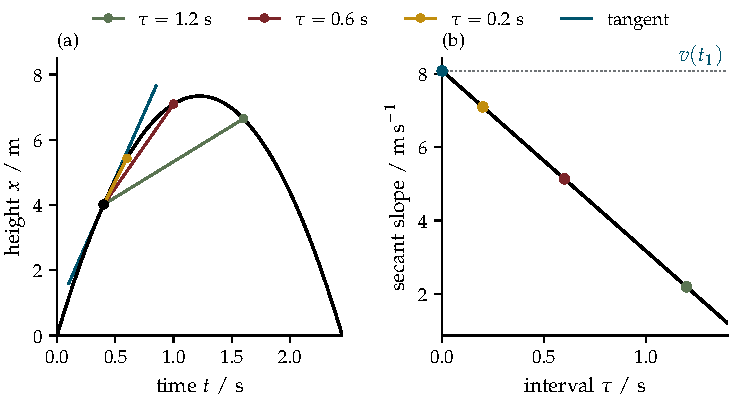
\includegraphics{ch01_motion/secant}
\caption{Velocity as a limit. (a) Height of the ball of
\cref{eq:mo-ball} against time, with secants from $t_1 = \SI{0.4}{\second}$
over three intervals $\tau$ and the tangent at $t_1$. (b) The slope of the
secant against $\tau$, which falls short of $v(t_1)$ by $g\tau/2$ and
reaches it as $\tau \to 0$.}
\label{fig:mo-secant}
\end{figure}

\subsection*{Velocity at an instant}

The velocity at the single instant $t_1$ cannot be found by setting $\tau
= 0$ in the quotient on the left of \cref{eq:mo-secant}, because both its
numerator and its denominator would then vanish and $0/0$ has no value.
Instead we ask what value the average approaches as the interval is made
shorter and shorter. In \cref{eq:mo-secant} the answer is plain: the term
$-\tfrac12 g\tau$ can be made as small as we please by choosing $\tau$
small enough, while the first two terms do not depend on $\tau$ at all,
so the average approaches $v_0 - g t_1$. This value is the limit of the
average as $\tau$ tends to zero, and we define it to be the velocity at
$t_1$,
\begin{equation*}
   v(t_1) = \lim_{\tau\to0}\frac{x(t_1+\tau) - x(t_1)}{\tau}
   = \frac{\dd x}{\dd t}\bigg|_{t_1} ,
\end{equation*}
where the vertical bar with $t_1$ means that the derivative is evaluated
at the instant $t = t_1$.
The velocity is therefore the derivative of the position with respect to
time. Geometrically, as $\tau$ shrinks the secant turns about the point
at $t_1$ until it lies along the tangent there (\cref{fig:mo-secant}a), so
the velocity is the slope of the tangent to the graph of $x(t)$. For the
ball, since $t_1$ can be any time,
\begin{equation*}
   v(t) = v_0 - g t ,
\end{equation*}
and at $t_1 = \SI{0.4}{\second}$ the ball is moving upwards at
\SI{8.077}{\metre\per\second}.

\begin{toolbox}[Derivatives of powers]
The calculation above is an instance of a general rule. For a power
$t^n$, with $n$ a whole number $1, 2, 3, \dots$, multiply out $(t+\tau)^n$, the product of $n$ identical factors
$(t+\tau)$. Each term of the result takes either $t$ or $\tau$ from every
factor. Taking $t$ from all $n$ factors gives $t^n$; taking $\tau$ from
exactly one factor, which can be any of the $n$, gives $n$ terms each
equal to $t^{n-1}\tau$; every other choice takes $\tau$ at least twice.
Hence
\begin{equation*}
   (t+\tau)^n = t^n + n t^{n-1}\tau
   + \tau^2\times(\text{terms in } t \text{ and } \tau) .
\end{equation*}
Subtracting $t^n$, dividing by $\tau$ and letting $\tau\to0$ removes
every term that still contains $\tau$, leaving
\begin{equation*}
   \frac{\dd}{\dd t}\,t^n = n\,t^{n-1}.
\end{equation*}
The derivative of a sum is the sum of the derivatives, and a constant
factor passes through unchanged, because the difference quotient has both
properties for every $\tau$. A constant $c$ has derivative zero, since its
difference quotient is $(c - c)/\tau = 0$ for every $\tau$. Applied to \cref{eq:mo-ball}, these rules
give $\dd(v_0 t)/\dd t = v_0$ and $\dd(\tfrac12 g t^2)/\dd t = \tfrac12 g
\times 2t = gt$, and hence $v = v_0 - gt$ once more.
\end{toolbox}

The sign of the velocity carries the direction of motion: it is positive
while the ball rises and negative while it falls. Its magnitude $\lvert
v\rvert$ is the speed, which says how fast the ball moves without saying
in which direction.

\notebook{01}{shrink the interval and watch the secant turn into the tangent}

%=============================================================================!
% 1.3  ACCELERATION                                                           !
%=============================================================================!
\section{Acceleration}
\label{sec:mo-acceleration}

Because the velocity of the ball changes during its flight, a further
quantity is needed to describe how quickly it changes. This is the
acceleration, the rate of change of velocity, defined from the velocity in
exactly the way that the velocity was defined from the position,
\begin{equation*}
   a(t) = \lim_{\tau\to0}\frac{v(t+\tau) - v(t)}{\tau}
   = \frac{\dd v}{\dd t} = \frac{\dd^2 x}{\dd t^2}.
\end{equation*}
The last form records that the acceleration is obtained by differentiating
the position twice. Derivatives with respect to time occur so often that
they are also written with dots over the symbol, one dot for each
derivative: $\dot{x} = \dd x/\dd t = v$ and $\ddot{x} = \dd^2x/\dd t^2 =
a$. The dimension of acceleration is that of a velocity divided by a time,
$\mathsf{L}\mathsf{T}^{-1}/\mathsf{T} = \mathsf{L}\mathsf{T}^{-2}$, and it
is measured in metres per second per second, \si{\metre\per\second
\squared}. For the ball, differentiating $v(t) = v_0 - gt$ term by term
gives zero for the constant $v_0$ and $-g$ for the term $-gt$, so
\begin{equation*}
   a(t) = -g
\end{equation*}
at every instant of the flight. \Cref{fig:mo-ball} shows the height, the
velocity and the acceleration on a common time axis.

\begin{figure}[tb]
\centering
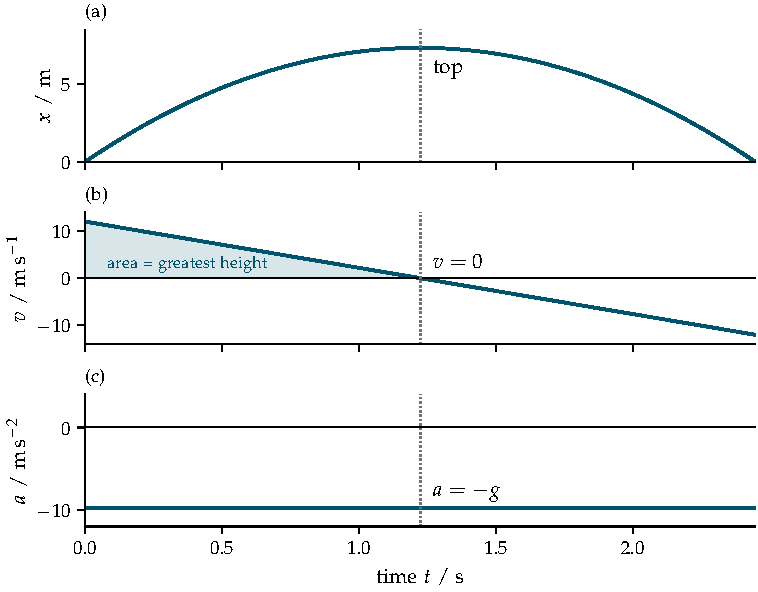
\includegraphics{ch01_motion/ball}
\caption{The thrown ball, $v_0 = \SI{12}{\metre\per\second}$. (a) Height,
(b) velocity and (c) acceleration against time. At the top of the flight
(dotted line) the velocity is zero and the acceleration is $-g$, as at
every other instant. The shaded area under $v(t)$ up to the top equals the
greatest height (\cref{sec:mo-integrating}).}
\label{fig:mo-ball}
\end{figure}

\subsection*{The top of the flight}

The ball reaches the top of its flight when it stops rising, that is, when
its velocity is zero. Setting $v(t) = 0$ and solving for $t$,
\begin{equation*}
   v_0 - g t = 0
   \quad\Longrightarrow\quad
   t = \frac{v_0}{g} = \frac{12}{9.80665}\,\si{\second}
   = \SI{1.224}{\second},
\end{equation*}
where the arrow $\Longrightarrow$ reads `which implies': the equation on
its right follows from the one on its left.
At this instant the ball is momentarily at rest, yet its acceleration is
still $-g$. There is no contradiction here, because a function can vanish
at an instant without its derivative vanishing at that instant. The
simplest example is $f(t) = t$, which is zero at $t = 0$ while its slope
there is 1. In the same way the velocity $v(t) = v_0 - gt$ is zero at $t =
v_0/g$, while its slope there, the acceleration, is $-g$. It is this
non-zero acceleration that carries the velocity from positive values,
through zero, to negative values, and it therefore turns the ball round.

\begin{keyidea}
Velocity is the rate of change of position, and acceleration is the rate
of change of velocity. Either can be zero at an instant at which the other
is not.
\end{keyidea}

\subsection*{Speeding up and slowing down}

The signs of $v$ and $a$ together determine whether a motion is speeding
up or slowing down. The speed is the size of the velocity, $\lvert
v\rvert$, and its square is $\lvert v\rvert^2 = v^2$. Since the speed is
never negative, it grows exactly when its square grows, and the square
spares us the absolute value. To see the rule, we therefore ask how $v^2$
changes in time. The square is a function of $v$, which is itself a
function of $t$, and the chain rule (below) gives
\begin{equation*}
   \frac{\dd}{\dd t}\,v^2 = 2v\,\frac{\dd v}{\dd t} = 2va .
\end{equation*}
When $v$ and $a$ have the same sign their product is positive, $v^2$
grows and the speed increases; when their signs differ the product is
negative and the speed decreases. While the ball rises, $v > 0$ and $a <
0$, so it slows down. Once it begins to fall, $v$ and $a$ are both
negative, and it speeds up.

\begin{toolbox}[The chain rule]
Let $f$ depend on $t$ through an intermediate quantity $u(t)$. Over a short
interval $\tau$, $u$ changes by $\Delta u = u(t+\tau) - u(t)$, and
multiplying and dividing by $\Delta u$,
\begin{equation*}
   \frac{f(u + \Delta u) - f(u)}{\tau}
   = \frac{f(u + \Delta u) - f(u)}{\Delta u}\times\frac{\Delta u}{\tau} .
\end{equation*}
As $\tau \to 0$, $\Delta u \to 0$ too, so the first factor approaches
$f'(u)$, the derivative of $f$ with respect to $u$, and the second
approaches $\dd u/\dd t$. At $\Delta u = 0$, define the first factor by
its limiting value $f'(u)$; its product with $\Delta u/\tau$ is then zero,
as is the left side. This also covers intervals on which $u$ does not
change. Hence
\begin{equation*}
   \frac{\dd}{\dd t}\,f\bigl(u(t)\bigr) = f'(u)\,\frac{\dd u}{\dd t}.
\end{equation*}
With $f(u) = u^2$, so that $f'(u) = 2u$, and $u = v$, this gives the rate
$2v\,\dd v/\dd t$ used above.
\end{toolbox}

\notebook{01}{move the time cursor along $x$, $v$ and $a$}

%=============================================================================!
% 1.4  FROM ACCELERATION BACK TO MOTION                                       !
%=============================================================================!
\section{From acceleration back to motion}
\label{sec:mo-integrating}

Differentiation takes us from position to velocity and from velocity to
acceleration. To predict a motion we need to travel in the opposite
direction, from a known acceleration back to the position, and the tool
for this is integration.

\subsection*{Displacement as an area}

Divide the time from $0$ to $t$ into many short intervals of length
$\Delta t$, and let $t_k$ be the start of the $k$th interval. Over an
interval short enough that the velocity hardly changes, the object moves
through approximately $v(t_k)\,\Delta t$, a velocity multiplied by a time.
The total displacement is the sum of these small contributions,
\begin{equation*}
   x(t) - x(0) \approx \sum_k v(t_k)\,\Delta t ,
\end{equation*}
where $\sum_k$, a capital Greek sigma for `sum', means that the
expression after it is added up for every interval $k = 1, 2, 3, \dots$
in turn. Each term $v(t_k)\,\Delta t$ is the area of a thin rectangle of height
$v(t_k)$ and width $\Delta t$ standing on the time axis. As $\Delta t \to
0$ the approximation becomes exact and the sum becomes an integral, the
area under the graph of $v$. The same argument applied to the velocity,
whose rate of change is $a$, gives the companion result, and together
\begin{equation}
   v(t) = v(0) + \int_0^t a(t')\,\dd t', \qquad
   x(t) = x(0) + \int_0^t v(t')\,\dd t' .
   \label{eq:mo-integrals}
\end{equation}
These are the fundamental theorem of calculus, which states that
integrating a derivative from $0$ to $t$ returns the change in the
original function. The variable of integration is written $t'$ to
distinguish it from the upper limit $t$. Where $v$ is negative the area
counts as negative, so the integral measures the signed displacement. For
the ball, the area under $v(t)$ from the throw to the top of the flight is
therefore the greatest height that it reaches, shaded in
\cref{fig:mo-ball}(b).

\Cref{eq:mo-integrals} also shows what is needed to determine a motion.
Each integration introduces a starting value, the velocity $v(0)$ in the
first and the position $x(0)$ in the second, and these do not follow from
the acceleration. Two balls subject to the same acceleration but thrown
at different speeds therefore follow different paths. When the
acceleration is known at every instant, and the initial position and
velocity are given, the two integrals determine the motion uniquely.
Predicting a motion thus reduces to finding its acceleration, and
Chapter~2 shows that the acceleration is supplied by forces.

\subsection*{Constant acceleration}

When the acceleration is a constant $a$, both integrals in
\cref{eq:mo-integrals} can be evaluated directly. Writing $x_0 = x(0)$ and
$v_0 = v(0)$, the first gives the velocity,
\begin{equation*}
   v(t) = v_0 + \int_0^t a\,\dd t' = v_0 + at ,
\end{equation*}
and substituting this velocity into the second gives the position,
\begin{equation*}
   x(t) = x_0 + \int_0^t \bigl(v_0 + a t'\bigr)\,\dd t'
   = x_0 + \Bigl[\, v_0 t' + \tfrac12 a t'^2 \Bigr]_0^t
   = x_0 + v_0 t + \tfrac12 a t^2 .
\end{equation*}
Together,
\begin{equation}
   v(t) = v_0 + at, \qquad x(t) = x_0 + v_0 t + \tfrac12 a t^2 ,
   \label{eq:mo-constant}
\end{equation}
and \cref{eq:mo-ball} is the particular case $x_0 = 0$ and $a = -g$.

These two equations both contain the time, but many questions concern only
where an object goes, not when it gets there: how high does the ball
rise, for instance, or how fast is it moving at a given height? A relation
free of $t$ answers such questions directly. Provided that $a \neq 0$, the
first equation gives $t = (v - v_0)/a$, and substituting this into the
second eliminates the time:
\begin{align*}
   x - x_0 &= v_0\,\frac{v - v_0}{a} + \frac{a}{2}\,
      \frac{(v - v_0)^2}{a^2}
      && \text{substituting for $t$}\\
   &= \frac{2v_0(v - v_0) + (v - v_0)^2}{2a}
      && \text{cancelling $a$; common denominator $2a$}\\
   &= \frac{(v - v_0)\,(2v_0 + v - v_0)}{2a}
      && \text{taking out $(v - v_0)$}\\
   &= \frac{(v - v_0)(v + v_0)}{2a} = \frac{v^2 - v_0^2}{2a}
      && \text{$2v_0 - v_0 = v_0$; difference of squares.}
\end{align*}
Multiplying both sides by $2a$ and rearranging,
\begin{equation}
   v^2 = v_0^2 + 2a(x - x_0) .
   \label{eq:mo-v2}
\end{equation}

For the ball, $x_0 = 0$ and $a = -g$, so \cref{eq:mo-v2} reads $v^2 =
v_0^2 - 2gx$. The ball stops rising where $v = 0$, which gives $0 = v_0^2
- 2gx$ and hence the greatest height
\begin{equation*}
   x_{\max} = \frac{v_0^2}{2g} = \frac{12^2}{2\times9.80665}\,\si{\metre}
   = \SI{7.342}{\metre}.
\end{equation*}
The ball returns to the hand when $x = 0$ again. Setting $x = 0$ in
\cref{eq:mo-ball} and taking out the common factor $t$,
\begin{equation*}
   0 = v_0 t - \tfrac12 g t^2 = t\,\bigl(v_0 - \tfrac12 g t\bigr),
\end{equation*}
which is satisfied at the throw, $t = 0$, and again at $t = 2v_0/g =
\SI{2.447}{\second}$, twice the time to the top. At that moment
\cref{eq:mo-v2} with $x = 0$ gives $v^2 = v_0^2$, so $v = \pm v_0$; since
the ball is then falling, $v = -v_0$, and it returns at the speed with
which it was thrown.

When the acceleration depends on the position, as it will for an atom
pushed by its neighbours, the integrand of \cref{eq:mo-integrals} contains
the very motion we are trying to find. Except for special force laws,
we cannot evaluate those integrals in closed form. A computer then
advances the motion through many short intervals instead, and
\cref{sec:mo-taylor} develops the mathematics that makes this possible,
once the trigonometric functions it relies on are in place.

\notebook{01}{the area under $v(t)$ up to the cursor}

%=============================================================================!
% 1.5  ANGLES AND THE TRIGONOMETRIC FUNCTIONS                                 !
%=============================================================================!
\section{Angles and the trigonometric functions}
\label{sec:mo-trig}

The motions met so far run along straight lines or arcs of a parabola. Many
of the motions that matter later turn or repeat: a wheel spinning, a block
bouncing on a spring, two bonded atoms vibrating, a molecule rotating. All
of them are described with angles and with the sine and cosine functions,
and this section builds those functions from the geometry of a circle,
together with every property of them that the book uses.

\subsection*{Measuring angles}

Consider a mark on the rim of a wheel of radius $r$. As the wheel turns
through some angle, the mark travels a distance $s$ along the rim, the
length of the arc. The size of the angle could be given in degrees, but
degrees are a convention, 360 to a full turn, chosen for their many
divisors. A more natural measure follows from the arc itself. Doubling the
angle doubles the arc, and doubling the radius at a fixed angle doubles it
too, so the ratio of arc to radius depends only on the angle. That ratio
defines the angle in radians,
\begin{equation*}
   \theta = \frac{s}{r} .
\end{equation*}
Being a length divided by a length, $\theta$ is a pure number, which is
what allows it to appear inside $\sin$ and $\cos$ (\cref{sec:mo-units}).
One full turn carries the mark once round the circumference, $s = 2\pi r$,
so a full turn is $2\pi$ radians. The two measures are therefore related by
$2\pi\ \text{rad} = \ang{360}$, and
\begin{equation*}
   \SI{1}{\radian} = \frac{\ang{180}}{\pi} \approx \ang{57.3}, \qquad
   \ang{90} = \frac{\pi}{2}, \qquad \ang{60} = \frac{\pi}{3}, \qquad
   \ang{45} = \frac{\pi}{4}, \qquad \ang{30} = \frac{\pi}{6} .
\end{equation*}
From here on, every angle is in radians unless degrees are stated.

\subsection*{Sine and cosine}

Draw a circle of radius 1, the unit circle, centred on the origin, and
mark the point $P$ reached by turning anticlockwise through an angle
$\theta$ from the point $(1, 0)$ on the positive $x$ axis
(\cref{fig:mo-trig}a). The coordinates of $P$ define the cosine and the
sine of $\theta$,
\begin{equation*}
   P = (\cos\theta,\ \sin\theta) .
\end{equation*}
For an angle between 0 and $\pi/2$, the line $OP$, the perpendicular from
$P$ to the $x$ axis and the axis itself form a right-angled triangle with hypotenuse 1,
so $\cos\theta$ is the adjacent side divided by the hypotenuse and
$\sin\theta$ the opposite side divided by the hypotenuse, the familiar
definitions from triangles. The circle definition has the advantage that
it works for every angle, including angles beyond a quarter turn, negative
angles and angles of more than a full turn. On a wheel of radius $r$ the
mark sits at $r(\cos\theta, \sin\theta)$, since scaling the unit circle
by $r$ scales both coordinates.

\begin{figure}[htb]
\centering
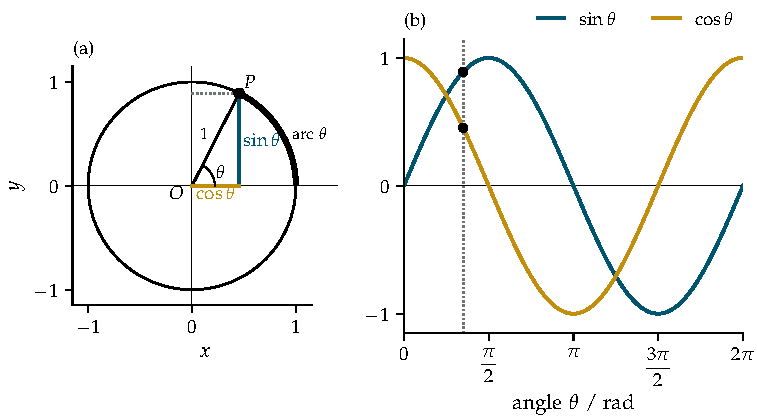
\includegraphics{ch01_motion/trig}
\caption{Sine and cosine from the circle. (a) The point $P$ at angle
$\theta = \SI{1.1}{\radian}$ (\ang{63}) on the unit circle has
coordinates $(\cos\theta, \sin\theta)$; the thick arc from $(1, 0)$ to
$P$ has length $\theta$. (b) The two coordinates against $\theta$ over one
full turn, with the values at $\theta = \SI{1.1}{\radian}$ marked.}
\label{fig:mo-trig}
\end{figure}

Plotting the two coordinates against the angle, as $P$ goes once round
the circle, unrolls the circle into the two waves of \cref{fig:mo-trig}(b).
Several properties follow directly from the picture.
\begin{itemize}
\item Since $P$ lies on a circle of radius 1, Pythagoras' theorem gives
   \begin{equation*}
      \cos^2\theta + \sin^2\theta = 1 ,
   \end{equation*}
   where $\cos^2\theta$ means $(\cos\theta)^2$. Both functions therefore
   lie between $-1$ and $1$.
\item Turning a further $2\pi$ brings $P$ back to where it was, so both
   functions repeat with period $2\pi$: $\sin(\theta + 2\pi) = \sin\theta$
   and $\cos(\theta + 2\pi) = \cos\theta$.
\item Turning clockwise instead of anticlockwise reflects $P$ in the $x$
   axis, which keeps its $x$ coordinate and reverses its $y$ coordinate:
   $\cos(-\theta) = \cos\theta$ and $\sin(-\theta) = -\sin\theta$.
\item Reflecting $P$ in the line $y = x$ swaps its coordinates. The
   reflection also turns the angle measured anticlockwise from the $x$ axis
   into the same angle measured clockwise from the $y$ axis, which itself
   lies at $\pi/2$, so the
   reflected point is at angle $\pi/2 - \theta$. Hence $\cos(\pi/2 - \theta)
   = \sin\theta$ and $\sin(\pi/2 - \theta) = \cos\theta$. Replacing $\theta$
   by $-\theta$ in the second and using the previous property gives
   $\sin(\theta + \pi/2) = \cos\theta$: the cosine is the sine shifted by a
   quarter turn, which is visible in \cref{fig:mo-trig}(b).
\item Reflecting $P$ in the $y$ axis keeps its $y$ coordinate, reverses its
   $x$ coordinate and carries $\theta$ to $\pi - \theta$, since the
   reflected point lies at angle $\theta$ measured clockwise from the
   negative $x$ axis, which is at $\pi$. Hence $\sin(\pi -
   \theta) = \sin\theta$ and $\cos(\pi - \theta) = -\cos\theta$.
\item At the quarter turns $P$ sits on an axis, giving $\sin 0 = 0$, $\cos
   0 = 1$, $\sin(\pi/2) = 1$, $\cos(\pi/2) = 0$, $\sin\pi = 0$ and $\cos\pi
   = -1$. At $\theta = \pi/4$ the point lies on the line $y = x$, so its two
   coordinates are equal, and $\cos^2 + \sin^2 = 1$ becomes $2\cos^2(\pi/4)
   = 1$; taking the positive root, since $P$ lies in the first quarter,
   both equal $1/\sqrt2$.
\end{itemize}
The tangent function, $\tan\theta = \sin\theta/\cos\theta$ (defined where
$\cos\theta \neq 0$), is the slope of the line $OP$; despite its name it
is not the tangent line of \cref{sec:mo-velocity}. Finally, the sine can
be undone. For a number $s$ between $-1$ and $1$, $\arcsin s$ is the angle
between $-\pi/2$ and $\pi/2$ whose sine is $s$. Because $\sin(\pi - \theta)
= \sin\theta$, the angle $\pi - \arcsin s$ has the same sine. When $0 < s
< 1$ these are the only two angles between 0 and $\pi$ with sine $s$,
since the horizontal line $y = s$ meets the upper half of the unit
circle at exactly two points;
when $s = 1$ the two coincide, since $\pi - \pi/2 = \pi/2$, and the
single angle in that range whose sine is 1 is $\pi/2$.

\subsection*{The addition formulae}

The sine and cosine of a sum of two angles are needed repeatedly, and they
follow from one observation: the distance between two points on a circle
does not change when the circle is turned. Let $P$ and $Q$ be the points
on the unit circle at angles $p$ and $q$. By Pythagoras' theorem, the
square of the distance between them is
\begin{align*}
   \lvert PQ\rvert^2 &= (\cos p - \cos q)^2 + (\sin p - \sin q)^2\\
   &= (\cos^2 p + \sin^2 p) + (\cos^2 q + \sin^2 q)
      - 2(\cos p\cos q + \sin p\sin q)\\
   &= 2 - 2(\cos p\cos q + \sin p\sin q),
\end{align*}
where the second line multiplies out the two squares and groups the
terms, and the third uses $\cos^2 + \sin^2 = 1$ for each angle.
Now turn the circle clockwise through $q$ (\cref{fig:mo-turn}). Turning
lowers the angle of every point by $q$, so $Q$ moves to angle 0, the point
$(1, 0)$, and $P$ moves to angle $p - q$. A turn moves the whole circle
rigidly, so the distance between $P$ and $Q$ is unchanged. Computing it
again from the new positions,
\begin{align*}
   \lvert PQ\rvert^2 &= \bigl(\cos(p-q) - 1\bigr)^2 + \sin^2(p-q)\\
   &= \cos^2(p-q) - 2\cos(p-q) + 1 + \sin^2(p-q)
      && \text{expanding the square}\\
   &= 2 - 2\cos(p-q)
      && \text{using $\cos^2 + \sin^2 = 1$.}
\end{align*}
\begin{figure}[htb]
\centering
\begin{tikzpicture}[scale=1.6, line cap=round]
   \def\p{118}\def\q{42}
   \foreach \shift/\a/\b/\name in {0/\p/\q/{}, 3.6/{\p-\q}/0/{\prime}}{
      \begin{scope}[xshift=\shift cm]
         \draw[black!35, line width=0.4pt] (-1.15,0) -- (1.15,0);
         \draw[black!35, line width=0.4pt] (0,-1.15) -- (0,1.15);
         \draw[line width=0.6pt] (0,0) circle (1);
         \draw[accent, line width=1pt] ({cos(\a)},{sin(\a)}) --
            ({cos(\b)},{sin(\b)});
         \draw[black!55, line width=0.4pt] (0,0) -- ({cos(\a)},{sin(\a)});
         \draw[black!55, line width=0.4pt] (0,0) -- ({cos(\b)},{sin(\b)});
         \fill ({cos(\a)},{sin(\a)}) circle (0.9pt);
         \fill ({cos(\b)},{sin(\b)}) circle (0.9pt);
         \node[above left] at ({cos(\a)},{sin(\a)}) {\small$P$};
         \node[right] at ({cos(\b)},{sin(\b)}) {\small$Q$};
      \end{scope}}
   \node[below] at (0,-1.18) {\small angles $p$ and $q$};
   \node[below] at (3.6,-1.18) {\small angles $p - q$ and $0$};
   \draw[-{Stealth[length=4pt]}, line width=0.5pt] (1.45,-0.35)
      to[bend right=30] node[below, yshift=-2pt, align=center]
      {\small turn through\\\small $q$ clockwise} (2.2,-0.35);
\end{tikzpicture}
\caption{The chord $PQ$ (teal) before and after the circle is turned
clockwise through $q$. Turning does not change its length, which gives
two expressions for $\lvert PQ\rvert^2$.}
\label{fig:mo-turn}
\end{figure}

Equating the two expressions for $\lvert PQ\rvert^2$ gives the first
addition formula,
\begin{equation*}
   \cos(p - q) = \cos p\cos q + \sin p\sin q .
\end{equation*}
The others follow from it. For the cosine of a sum,
\begin{align*}
   \cos(p+q) &= \cos p\cos(-q) + \sin p\sin(-q)
      && \text{replacing $q$ by $-q$}\\
   &= \cos p\cos q - \sin p\sin q
      && \text{as $\cos(-q) = \cos q$, $\sin(-q) = -\sin q$.}
\end{align*}
For the sine,
\begin{align*}
   \sin(p+q) &= \cos\bigl(\pi/2 - (p+q)\bigr)
      && \text{as $\sin\theta = \cos(\pi/2 - \theta)$}\\
   &= \cos\bigl((\pi/2 - p) - q\bigr)
      && \text{regrouping the angle}\\
   &= \cos(\pi/2 - p)\cos q + \sin(\pi/2 - p)\sin q
      && \text{first addition formula}\\
   &= \sin p\cos q + \cos p\sin q
      && \text{quarter-turn relations,}
\end{align*}
and replacing $q$ by $-q$ as before gives $\sin(p-q) = \sin p\cos q -
\cos p\sin q$. Together,
\begin{equation}
\begin{aligned}
   \cos(p \pm q) &= \cos p\cos q \mp \sin p\sin q ,\\
   \sin(p \pm q) &= \sin p\cos q \pm \cos p\sin q ,
\end{aligned}
\label{eq:mo-addition}
\end{equation}
with the upper signs taken together and the lower signs together. Setting
$q = p$ gives the double-angle formulae $\sin 2p = 2\sin p\cos p$ and
$\cos 2p = \cos^2 p - \sin^2 p$.

\subsection*{The derivatives of sine and cosine}

To differentiate $\sin\theta$ we need the limit of the difference quotient
$[\sin(\theta + h) - \sin\theta]/h$ as $h \to 0$. Expanding the first term
with \cref{eq:mo-addition},
\begin{equation*}
   \frac{\sin(\theta+h) - \sin\theta}{h}
   = \frac{\sin\theta\cos h + \cos\theta\sin h - \sin\theta}{h}
   = \cos\theta\,\frac{\sin h}{h} - \sin\theta\,\frac{1 - \cos h}{h} ,
\end{equation*}
where the second step takes out the factor $-\sin\theta$ from the first
and third terms of the numerator, $\sin\theta\cos h - \sin\theta =
-\sin\theta\,(1 - \cos h)$, and divides each part by $h$ separately. So
the derivative depends on two limits, those of $\sin h/h$ and $(1 -
\cos h)/h$ as $h \to 0$. Neither can be found by setting $h = 0$, which
gives $0/0$ in both.

The first limit follows from comparing three areas in
\cref{fig:mo-squeeze}, for an angle $h$ with $0 < h < \pi/2$. The point $A$
is $(1, 0)$, $P$ is the point at angle $h$ on the unit circle, and $T$ is
where the line $OP$, extended, meets the vertical line through $A$; since
$OP$ has slope $\tan h$, the length $AT$ is $\tan h$. The triangle $OAP$
has base 1 and height $\sin h$, so its area is $\tfrac12\sin h$. The
sector $OAP$, the slice of the disc bounded by the arc, is the fraction
$h/2\pi$ of the whole disc of area $\pi$, so its area is $\tfrac12 h$;
this is where measuring $h$ in radians matters. The larger triangle $OAT$
has base 1 and height $\tan h$, so its area is $\tfrac12\tan h$. Each
region contains the one before, so
\begin{equation*}
   \tfrac12\sin h \le \tfrac12 h \le \tfrac12\tan h .
\end{equation*}
Multiplying by $2/\sin h$, which is positive, and using $\tan h = \sin
h/\cos h$, this becomes
\begin{equation*}
   1 \le \frac{h}{\sin h} \le \frac{1}{\cos h} .
\end{equation*}
As $h \to 0$, the point $P$ slides along the circle to $A = (1, 0)$, so
$\cos h \to 1$ and $\sin h \to 0$, and the middle quantity is squeezed between
two quantities that both approach 1, and must approach 1 itself; the same
then holds for its reciprocal, $\sin h/h \to 1$. For negative $h$,
$\sin(-h)/(-h) = \sin h/h$, since the sine reverses sign with its angle,
so the same limit holds from both sides. For the second limit,
multiplying numerator and denominator by $1 + \cos h$ and using $1 -
\cos^2 h = \sin^2 h$,
\begin{equation*}
   \frac{1 - \cos h}{h} = \frac{1 - \cos^2 h}{h\,(1 + \cos h)}
   = \frac{\sin h}{h}\cdot\frac{\sin h}{1 + \cos h}
   \;\longrightarrow\; 1\times\frac{0}{2} = 0 .
\end{equation*}

\begin{figure}[htb]
\centering
\begin{tikzpicture}[scale=3.4, line cap=round]
   \def\h{35}
   \coordinate (O) at (0,0);
   \coordinate (A) at (1,0);
   \coordinate (P) at ({cos(\h)},{sin(\h)});
   \coordinate (T) at (1,{tan(\h)});
   \fill[accent!12] (O) -- (A) -- (T) -- cycle;
   \fill[accent!32] (O) -- (A) arc[start angle=0, end angle=\h, radius=1]
      -- cycle;
   \fill[accent!55] (O) -- (A) -- (P) -- cycle;
   \draw[black!45, line width=0.4pt] (0,0) -- (1.18,0);
   \draw[black!45, line width=0.4pt] ({cos(\h)},0) -- (P);
   \draw[line width=0.8pt] (O) -- (T) -- (A) -- cycle;
   \draw[line width=0.8pt] (A) arc[start angle=0, end angle=\h, radius=1];
   \draw[line width=0.5pt] (O) -- (P) -- (A);
   \draw[line width=0.4pt] (0.18,0) arc[start angle=0, end angle=\h,
      radius=0.18];
   \node at ({0.25*cos(\h/2)},{0.25*sin(\h/2)}) {\small$h$};
   \node[below left] at (O) {\small$O$};
   \node[below right] at (A) {\small$A$};
   \node[above left] at (P) {\small$P$};
   \node[right] at (T) {\small$T$};
   \node[right, black!70] at (1,{tan(\h)/2}) {\small$\tan h$};
   \node[left, white, xshift=-1pt] at ({cos(\h)},{sin(\h)/2})
      {\small$\sin h$};
   \node[below] at (0.5,0) {\small$1$};
\end{tikzpicture}
\caption{The three nested regions that bound $\sin h/h$. The triangle
$OAP$ (darkest) lies inside the sector $OAP$, which adds the sliver
between the chord $PA$ and the arc (medium); the sector lies inside the
triangle $OAT$ (lightest), where $T$ lies on $OP$ extended. Their areas
are $\tfrac12\sin h$, $\tfrac12 h$ and $\tfrac12\tan h$.}
\label{fig:mo-squeeze}
\end{figure}

Returning to the difference quotient, the first limit turns $\cos\theta
\sin h/h$ into $\cos\theta$ and the second removes the term in $\sin
\theta$, so
\begin{equation}
   \frac{\dd}{\dd\theta}\sin\theta = \cos\theta, \qquad
   \frac{\dd}{\dd\theta}\cos\theta = -\sin\theta ,
   \label{eq:mo-trig-derivs}
\end{equation}
where the second follows in the same way from the formula for
$\cos(\theta + h)$:
\begin{equation*}
   \frac{\cos(\theta+h) - \cos\theta}{h}
   = -\sin\theta\,\frac{\sin h}{h} - \cos\theta\,\frac{1 - \cos h}{h}
   \;\longrightarrow\; -\sin\theta .
\end{equation*}
Had the angle been measured in degrees, the sector area would have
carried a factor $\pi/180$ and so would both derivatives, which is why
radians are used throughout. The derivatives also agree with
\cref{fig:mo-trig}(b): the sine rises most steeply where the cosine is
largest, falls most steeply where the cosine is smallest, and is flat
where the cosine is zero.

\subsection*{Sinusoids}

A quantity that varies in time as
\begin{equation}
   x(t) = A\sin(\omega t + \phi)
   \label{eq:mo-sinusoid}
\end{equation}
is called a sinusoid, and three constants describe it
(\cref{fig:mo-sinusoid}). The amplitude $A$, taken positive, is the
largest value that $x$ reaches, since the sine never exceeds 1 and does
reach it. The angular frequency $\omega$,
in radians per second, sets how quickly the argument $\omega t + \phi$
advances, and since the sine repeats when its argument grows by $2\pi$,
the motion repeats after a time $2\pi/\omega$, the period. The number of
repetitions per second is one divided by the period, $\omega/2\pi$, the
frequency, measured in hertz,
where one hertz is one repetition per second, $\SI{1}{\hertz} =
\SI{1}{\per\second}$. The phase $\phi$ sets where in its cycle the motion starts:
writing $\omega t + \phi = \omega(t + \phi/\omega)$ shows that $x$ does
at time $t$ what $A\sin\omega t$ does at the later time $t + \phi/\omega$,
so every crest arrives earlier by $\phi/\omega$. With $\phi = \pi/2$ the
sinusoid becomes $A\cos\omega t$, by the quarter-turn relation. By the
chain rule of \cref{sec:mo-acceleration} and \cref{eq:mo-trig-derivs}, the
velocity and acceleration of a sinusoid are
\begin{equation*}
   \dot{x} = A\omega\cos(\omega t + \phi), \qquad
   \ddot{x} = -A\omega^2\sin(\omega t + \phi) = -\omega^2 x .
\end{equation*}
The velocity is again a sinusoid. Since $\cos\theta = \sin(\theta +
\pi/2)$, the velocity can be written as $A\omega\sin(\omega t + \phi +
\pi/2)$, a
sinusoid whose phase is larger by $\pi/2$, so its crests come earlier by
$(\pi/2)/\omega$, a quarter of the period. The acceleration is always
proportional to $x$ and opposite to it. This last property will reappear in \cref{sec:mo-circle} and again in Chapter~4.

\begin{figure}[htb]
\centering
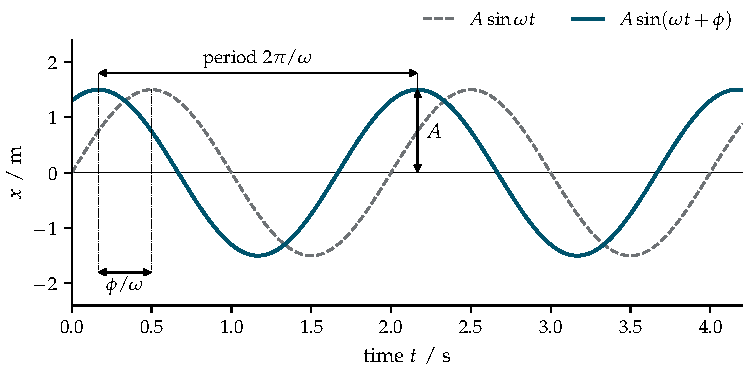
\includegraphics{ch01_motion/sinusoid}
\caption{A sinusoid $x(t) = A\sin(\omega t + \phi)$ with $A =
\SI{1.5}{\metre}$, $\omega = \pi\ \si{\radian\per\second}$ (period
\SI{2}{\second}) and $\phi = \pi/3$, against $A\sin\omega t$ (dashed).
Every crest of the shifted wave arrives earlier by $\phi/\omega =
\SI{0.333}{\second}$.}
\label{fig:mo-sinusoid}
\end{figure}

\notebook{01}{turn the unit circle and watch $\sin\theta$ and $\cos\theta$; shape a sinusoid}

%=============================================================================!
% 1.6  MOTION IN A PLANE AND IN SPACE                                         !
%=============================================================================!
\section{Motion in a plane and in space}
\label{sec:mo-plane}

Most motion does not take place along a single line, and positions must
then be described by vectors. A position in space is a vector $\vb{r} =
(x, y, z)$ measured from a chosen origin, and a moving object traces out a
curve $\vb{r}(t)$, its path. The box below collects the properties of
vectors that the book uses.

\begin{toolbox}[Vectors]
A vector $\vb{a} = (a_x, a_y, a_z)$ is added to another, or multiplied by
a number, component by component. Drawn as an arrow from the origin to
the point $(a_x, a_y, a_z)$, a vector has a length and a direction.
Multiplying it by a positive number scales its length and keeps its
direction, and a negative number also reverses the direction. The
difference $\vb{b} - \vb{a}$ is the arrow from the tip of $\vb{a}$ to the
tip of $\vb{b}$, since adding it to $\vb{a}$ gives $\vb{b}$. Its length, or magnitude, follows from
Pythagoras' theorem applied twice, first in the $xy$ plane and then with
the $z$ component, $\lvert\vb{a}\rvert = (a_x^2 + a_y^2 + a_z^2)^{1/2}$.
The scalar product, or dot product, of two vectors is the number
\begin{equation*}
   \vb{a}\cdot\vb{b} = a_x b_x + a_y b_y + a_z b_z ,
\end{equation*}
so that $\vb{a}\cdot\vb{a} = \lvert\vb{a}\rvert^2$. Expanding
$\lvert\vb{a} - \vb{b}\rvert^2 = (a_x - b_x)^2 + (a_y - b_y)^2 + (a_z -
b_z)^2$ gives $\lvert\vb{a}\rvert^2 + \lvert\vb{b}\rvert^2 - 2\,\vb{a}
\cdot\vb{b}$, so
\begin{equation*}
   \vb{a}\cdot\vb{b} = \tfrac12\bigl(\lvert\vb{a}\rvert^2
   + \lvert\vb{b}\rvert^2 - \lvert\vb{a} - \vb{b}\rvert^2\bigr)
\end{equation*}
depends only on lengths, and is therefore unchanged when the axes are
turned. We may then turn the axes until both vectors lie in the $xy$
plane, and its geometric meaning follows from the addition formulae of
\cref{sec:mo-trig}. Write the two vectors in terms of their lengths and
the angles $\alpha$ and $\beta$ that they make with the $x$ axis, $\vb{a}
= \lvert\vb{a}\rvert(\cos\alpha, \sin\alpha)$ and $\vb{b} =
\lvert\vb{b}\rvert(\cos\beta, \sin\beta)$. Then
\begin{equation*}
   \vb{a}\cdot\vb{b}
   = \lvert\vb{a}\rvert\lvert\vb{b}\rvert\,(\cos\alpha\cos\beta
     + \sin\alpha\sin\beta)
   = \lvert\vb{a}\rvert\lvert\vb{b}\rvert\cos(\alpha - \beta),
\end{equation*}
and $\alpha - \beta$ is the angle between the vectors (or its negative,
or that plus a full turn; since the cosine is even and has period $2\pi$,
the value is the same). The scalar product
is therefore the product of the two lengths and the cosine of the angle
between them. In particular, two non-zero vectors are perpendicular
exactly when their scalar product is zero, since $\cos(\pi/2) = 0$.
\end{toolbox}

Velocity and acceleration are defined as before, now as vectors,
\begin{equation*}
   \vb{v} = \frac{\dd\vb{r}}{\dd t}
   = \biggl(\frac{\dd x}{\dd t}, \frac{\dd y}{\dd t},
   \frac{\dd z}{\dd t}\biggr), \qquad
   \vb{a} = \frac{\dd\vb{v}}{\dd t} = \frac{\dd^2\vb{r}}{\dd t^2},
\end{equation*}
so that each component is differentiated separately and obeys the
one-dimensional results of the preceding sections. The speed is the length
of the velocity vector, $v = \lvert\vb{v}\rvert$.

\subsection*{The velocity follows the path}

Over a short interval $\tau$ the object moves from $\vb{r}(t)$ to
$\vb{r}(t+\tau)$, and the vector $\vb{r}(t+\tau) - \vb{r}(t)$ joining the
two positions is a chord of the path. Dividing it by the positive number
$\tau$ changes its length but not its direction, and by the definition of
the derivative the quotient approaches $\vb{v}(t)$ as $\tau \to 0$. At the
same time the chord shrinks towards the point $\vb{r}(t)$ and turns into
the tangent to the path there; indeed, the direction the chord approaches
is what we mean by the tangent to a curve in space. The velocity is
therefore directed along
the tangent, in the direction of motion, whenever it is non-zero. No such
argument applies to the acceleration, which may point in any direction
relative to the path.

\subsection*{The projectile}

A ball thrown with speed $v_0$ at an angle $\alpha$ above the horizontal,
with $0 < \alpha < \pi/2$ so that it sets off both forwards and upwards,
illustrates this distinction. We take $x$ horizontal and $y$ vertical,
with the ball launched from the origin. With air resistance negligible,
its acceleration is observed to be $\vb{a} = (0, -g)$, the same $-g$ as
for the ball thrown straight up and nothing horizontally (Chapter~2
explains why), constant and directed downwards
(the motion stays in the vertical $xy$ plane, so the $z$ components are
zero and are dropped).
Its initial velocity has length $v_0$ and makes the angle $\alpha$ with
the $x$ axis, so by the definition of sine and cosine its components are
$v_0\cos\alpha$ horizontally and $v_0\sin\alpha$ vertically.
\Cref{eq:mo-constant} therefore applies to each component separately,
with $a = 0$ horizontally and $a = -g$ vertically,
\begin{equation*}
   x(t) = v_0\cos\alpha\; t, \qquad
   y(t) = v_0\sin\alpha\; t - \tfrac12 g t^2 .
\end{equation*}
The horizontal motion is uniform, while the vertical motion is that of the
ball of \cref{sec:mo-velocity} thrown upwards at $v_0\sin\alpha$, and
neither component affects the other.

The shape of the path follows from eliminating $t$. The first equation
gives $t = x/(v_0\cos\alpha)$, a division that needs $\cos\alpha \neq
0$; a ball thrown straight up, $\alpha = \pi/2$, never leaves the line
$x = 0$ and is the ball of \cref{sec:mo-velocity}. Substituting for $t$
in the second equation,
\begin{align*}
   y &= v_0\sin\alpha\,\frac{x}{v_0\cos\alpha}
      - \frac{g}{2}\,\frac{x^2}{v_0^2\cos^2\alpha}
      && \text{substituting for $t$}\\
   &= x\tan\alpha - \frac{g\,x^2}{2v_0^2\cos^2\alpha}
      && \text{using $\sin\alpha/\cos\alpha = \tan\alpha$,}
\end{align*}
a parabola opening downwards. The ball returns to its launch height when
$y = 0$; taking out the factor $t$ from $y(t)$ gives $t\,(v_0\sin\alpha -
\tfrac12 g t) = 0$, so the flight lasts $t = 2v_0\sin\alpha/g$. In that
time the ball travels the horizontal distance
\begin{equation*}
   d = v_0\cos\alpha\times\frac{2v_0\sin\alpha}{g}
   = \frac{v_0^2\,(2\sin\alpha\cos\alpha)}{g}
   = \frac{v_0^2\sin 2\alpha}{g},
\end{equation*}
its range, where the last step uses the double-angle formula of
\cref{sec:mo-trig}. Since $\sin2\alpha$ is at most 1, with that value
reached when $2\alpha = \pi/2$, the range is greatest at $\alpha = \pi/4$,
or \ang{45}. For $v_0 = \SI{12}{\metre\per\second}$ the range is
$144\sin\ang{120}/9.80665 = \SI{12.717}{\metre}$ at a launch angle of
\ang{60}, and $144/9.80665 = \SI{14.684}{\metre}$ at \ang{45}.

\Cref{fig:mo-plane}(a) shows the velocity turning to follow the path while
the acceleration continues to point downwards. The vertical component of
the velocity, $v_0\sin\alpha - gt$, vanishes at $t = v_0\sin\alpha/g$,
halfway through the flight, so at the top of the path the velocity is
horizontal, and its scalar product with the downward acceleration is
zero.

\begin{figure}[htb]
\centering
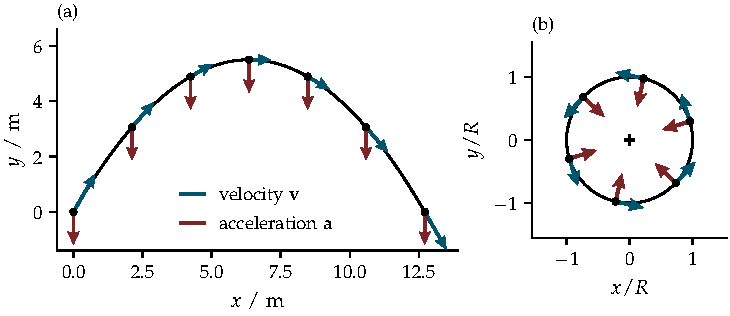
\includegraphics{ch01_motion/plane}
\caption{Velocity (teal) and acceleration (red) along two paths. (a) A
projectile launched at \SI{12}{\metre\per\second}, \ang{60} above the
horizontal, at seven equally spaced times. (b) Uniform motion on a circle
of radius $R$ (\cref{sec:mo-circle}). Arrow lengths are proportional to
the quantities they represent, on different scales for velocity and
acceleration.}
\label{fig:mo-plane}
\end{figure}

\notebook{01}{launch a projectile with chosen speed and angle}

%=============================================================================!
% 1.7  CIRCULAR MOTION                                                        !
%=============================================================================!
\section{Circular motion}
\label{sec:mo-circle}

A stone whirled on a string at a steady rate moves around a circle of
radius $R$, centred on the origin, at constant speed. Its angle from the
$x$ axis grows at a steady rate $\omega$, the angular speed in radians
per second, and we start the clock as it crosses the positive $x$ axis,
so that the angle is $\omega t$ at time $t$. By the definition of sine and cosine in
\cref{sec:mo-trig}, scaled to a circle of radius $R$, the position of the
stone is
\begin{equation*}
   \vb{r}(t) = R\,(\cos\omega t,\ \sin\omega t) ,
\end{equation*}
and it completes one revolution when $\omega t$ has grown by $2\pi$, in
the period $2\pi/\omega$.

\subsection*{Velocity and acceleration}

Each component is a sinusoid, and the chain rule with the derivatives of
\cref{eq:mo-trig-derivs} gives
\begin{equation*}
   \frac{\dd}{\dd t}\cos\omega t = -\omega\sin\omega t, \qquad
   \frac{\dd}{\dd t}\sin\omega t = \omega\cos\omega t .
\end{equation*}
Differentiating the position once and then a second time therefore gives
\begin{equation}
   \vb{v}(t) = R\omega\,(-\sin\omega t,\ \cos\omega t), \qquad
   \vb{a}(t) = -R\omega^2\,(\cos\omega t,\ \sin\omega t) = -\omega^2\vb{r}(t).
   \label{eq:mo-circle}
\end{equation}
The scalar product of the velocity with the position is
\begin{equation*}
   \vb{v}\cdot\vb{r} = R^2\omega\,\bigl(-\sin\omega t\cos\omega t
   + \cos\omega t\sin\omega t\bigr) = 0 ,
\end{equation*}
so the velocity is perpendicular to the radius and hence tangent to the
circle, as \cref{sec:mo-plane} requires. Its magnitude is
\begin{equation*}
   v = R\omega\,\bigl(\sin^2\omega t + \cos^2\omega t\bigr)^{1/2} = R\omega ,
\end{equation*}
which does not change in time. The radian, being a ratio of lengths,
drops out of the units, so $R\omega$ is in metres per second. The
acceleration $-\omega^2\vb{r}$ points
from the stone towards the centre, opposite to the position vector, with
magnitude $\omega^2 R$. Since $\omega = v/R$, this magnitude can also be
written $\omega^2 R = v^2/R$ (\cref{fig:mo-plane}b). A stone on a string
of \SI{0.5}{\metre} going round twice a second, for example, has $\omega
= 2\times2\pi = \SI{12.57}{\radian\per\second}$, a speed of
$\SI{6.28}{\metre\per\second}$ and an acceleration of
$\SI{79}{\metre\per\second\squared}$ towards the centre, about eight
times $g$.

\subsection*{Constant speed with non-zero acceleration}

Uniform circular motion therefore has a constant speed but a non-zero
acceleration at every instant, because acceleration measures any change of
velocity, including a change of direction alone. The relation between
speed and acceleration found in \cref{sec:mo-acceleration} extends to
vectors. Writing $v^2 = \vb{v}\cdot\vb{v} = v_x^2 + v_y^2 + v_z^2$ and
applying that result to each component,
\begin{equation*}
   \frac{\dd}{\dd t}\bigl(v_x^2 + v_y^2 + v_z^2\bigr)
   = 2v_x a_x + 2v_y a_y + 2v_z a_z = 2\,\vb{v}\cdot\vb{a} .
\end{equation*}
The speed is therefore constant over an interval exactly when
$\vb{v}\cdot\vb{a} = 0$ at every instant of that interval, which is the
case on the circle. On the parabola of \cref{sec:mo-plane}, by contrast,
$\vb{v}\cdot\vb{a} = v_0\cos\alpha\times0 + (v_0\sin\alpha - gt)(-g) =
-g\,v_y$, where $v_y = v_0\sin\alpha - gt$ is the vertical velocity. This
is negative while the ball rises ($v_y > 0$) and positive while it falls,
so the ball slows as it rises and speeds up as it falls; only at the top
is it zero.

\subsection*{The projection onto a line}

The $x$ coordinate of the stone, the projection of its motion onto the $x$
axis, moves back and forth along a line as $x(t) = R\cos\omega t$, a
sinusoid of amplitude $R$ and angular frequency $\omega$. The $x$
component of \cref{eq:mo-circle} gives this projection the acceleration
$-R\omega^2\cos\omega t$, which is $-\omega^2$ times $x(t)$ itself:
\begin{equation*}
   \frac{\dd^2 x}{\dd t^2} = -\omega^2 x ,
\end{equation*}
the property of every sinusoid found in \cref{sec:mo-trig}. The
acceleration of the projection is proportional to its distance from the
centre and directed back towards it, so it is greatest at the ends of the
swing and zero as it passes through the middle. \Cref{sec:ne-spring}
shows that a block attached to a spring obeys this equation, and
Chapter~4 that the small vibrations of atoms obey it to a good
approximation.

\notebook{01}{circular motion and its projection}

%=============================================================================!
% 1.8  SHORT INTERVALS AND THE TAYLOR SERIES                                  !
%=============================================================================!
\section{Short intervals and the Taylor series}
\label{sec:mo-taylor}

For the ball, the acceleration was constant and the integrals of
\cref{sec:mo-integrating} could be done by hand. For most motions, and for
general systems of interacting atoms, the acceleration changes from
moment to moment and the integrals cannot be done in closed form. A
computer then advances the motion through many short intervals, and on
each interval it needs an approximation to the position a short time
$\tau$ ahead, built from what is known at the start of the interval. The
Taylor series provides that approximation, and tells us how large its
error is.

\subsection*{Matching a polynomial to a function}

Near a time $t$, we look for a polynomial in $\tau$ that matches $x(t +
\tau)$ as closely as possible,
\begin{equation*}
   x(t+\tau) \approx c_0 + c_1\tau + c_2\tau^2 + c_3\tau^3 + \dotsb ,
\end{equation*}
and we choose its coefficients so that the polynomial and the function
have the same value, the same first derivative, the same second
derivative, and so on, at $\tau = 0$. Each condition fixes one
coefficient.
\begin{itemize}
\item Setting $\tau = 0$ leaves only $c_0$, so $c_0 = x(t)$.
\item Differentiating once with respect to $\tau$ gives $c_1 + 2c_2\tau +
   3c_3\tau^2 + \dotsb$, which at $\tau = 0$ is $c_1$. The function's own
   derivative with respect to $\tau$, with $t$ held fixed, is by the chain
   rule with inner function $u = t + \tau$, whose derivative with respect
   to $\tau$ is 1, $\dot{x}(t+\tau)$; repeating this, its $n$th derivative
   is $x^{(n)}(t+\tau)$, the $n$th derivative of $x$ evaluated at
   $t+\tau$. At $\tau = 0$ the first derivative is $\dot{x}(t)$, so matching
   gives $c_1 = \dot{x}(t)$.
\item Differentiating twice gives $2c_2 + 6c_3\tau + \dotsb$, which at
   $\tau = 0$ is $2c_2$, so $c_2 = \ddot{x}(t)/2$.
\item Differentiating three times gives $6c_3 + \dotsb$, so $c_3 =
   \dddot{x}(t)/6$, where $\dddot{x}$ is the third derivative.
\end{itemize}
Each differentiation brings down one more factor from the power of
$\tau$, so the $n$th differentiation of $c_n\tau^n$ produces $n\times(n-1)
\times\dotsb\times 1 = n!$ times $c_n$, a product written $n!$ and read
`$n$ factorial'. After $n$ differentiations the lower powers of $\tau$ have
become zero and the higher ones still contain $\tau$, so at $\tau = 0$ only
$n!\,c_n$ survives, and matching the $n$th derivative $x^{(n)}(t)$ gives
$c_n = x^{(n)}(t)/n!$. Collecting the coefficients gives the Taylor
series,
\begin{equation*}
   x(t+\tau) = \sum_{n=0}^{\infty} \frac{x^{(n)}(t)}{n!}\,\tau^n
   = x(t) + \dot{x}(t)\,\tau + \frac{\ddot{x}(t)}{2}\,\tau^2
   + \frac{\dddot{x}(t)}{6}\,\tau^3 + \dotsb ,
\end{equation*}
with $0! = 1$. For the functions met in this book, polynomials, sines,
cosines and exponentials, the infinite series converges to $x(t+\tau)$:
adding more and more terms brings the sum as close to $x(t+\tau)$ as we
please.
In general, matching derivatives guarantees only that the series stopped
after a finite number of terms has a small error, as described below, and
that is all the book relies on. For a motion, $\dot{x} = v$ and $\ddot{x}
= a$, so
\begin{equation}
   x(t+\tau) = x(t) + v(t)\,\tau + \tfrac12 a(t)\,\tau^2
   + \tfrac16\,\dddot{x}(t)\,\tau^3 + \order{\tau^4} .
   \label{eq:mo-taylor}
\end{equation}

\subsection*{The size of the error}

The symbol $\order{\tau^4}$ stands for everything left out, and it
records how quickly that remainder vanishes as the interval shrinks: a
quantity is $\order{\tau^4}$, read `of order $\tau^4$', if its absolute
value is no larger than some fixed constant times $\lvert\tau\rvert^4$
once $\lvert\tau\rvert$ is small enough. More generally, stopping the
series after the term in $\tau^n$ leaves an error of order $\tau^{n+1}$
for a smooth function, one that can be differentiated as often as we
like. To see why, call the error $D(\tau)$, the function $x(t+\tau)$
minus the polynomial of degree $n$, and take $\tau > 0$. By construction
$D$ and its first $n$ derivatives with respect to $\tau$ vanish at $\tau
= 0$. Since $n + 1$ differentiations remove a polynomial of degree $n$
entirely, the $(n+1)$th derivative of $D$ is $x^{(n+1)}(t+\tau)$. Let $M$
be the greatest value of $\lvert x^{(n+1)}\rvert$ between $t$ and $t +
\tau$. By \cref{eq:mo-integrals} the $n$th derivative of $D$, which
starts at zero, is the integral of the $(n+1)$th from 0 to $\tau$, an
area under a curve lying between $-M$ and $M$, so its size is at most
$M\tau$. Integrating again, the size of the $(n-1)$th derivative is at
most $\int_0^\tau M s\,\dd s = M\tau^2/2$. Each further integration raises
the power by one and divides by the new power, so after $n + 1$
integrations
\begin{equation*}
   \lvert D(\tau)\rvert \le \frac{M\,\lvert\tau\rvert^{n+1}}{(n+1)!} ,
\end{equation*}
and the same argument holds for $\tau < 0$. Halving the interval
therefore divides this bound by $2^{n+1}$, and the error itself by about
that factor.

\begin{toolbox}[Logarithmic axes]
Errors such as these span many powers of ten, so they are plotted on
logarithmic axes, on which the marks $10^{-3}$, $10^{-2}$ and $10^{-1}$
are equally spaced. Equal distances along such an axis stand for equal
ratios, here a factor of ten, rather than equal differences: the
position of a positive number $y$ along the axis is proportional to its
logarithm $\log y$, the power to which 10 must be raised to give $y$, so
that $\log 10^k = k$. Writing $y = 10^a$ and $z = 10^b$, so that $yz =
10^a\times10^b = 10^{a+b}$, gives $\log(yz) = a + b = \log y + \log z$:
the logarithm turns products into sums. Since $(10^a)^p = 10^{pa}$, it
also turns a power into a multiple, $\log(\tau^p) = p\log\tau$. An error
$D$ that behaves as $D = C\tau^p$ therefore obeys
\begin{equation*}
   \log D = \log C + p\log\tau ,
\end{equation*}
which is a straight line when $\log D$ is plotted against $\log\tau$.
Its slope is the power $p$: a line that rises by one power of ten for
every power of ten in $\tau$ has $p = 1$, and one that rises by four has
$p = 4$. The constant $C$ only moves the line up or down. The slope of an
error plot thus gives the power with which the error falls, and two
lines of equal slope differ only by a constant factor.
\end{toolbox}

\Cref{fig:mo-taylor} shows these properties for $x(t) = \sin t$ expanded
about $t_1 = \pi/4$. By \cref{eq:mo-trig-derivs} the derivatives of the
sine cycle through $\sin, \cos, -\sin, -\cos$, so at $\pi/4$ every one of
them is $\pm 1/\sqrt2$, and none is zero, so the leading term
$x^{(n+1)}(t_1)\,\tau^{n+1}/(n+1)!$ of every error is present. The
polynomial of degree 1 is the tangent line,
the polynomial of degree 2 adds the bending of the graph, and each further
degree follows the function over a wider range. Close to $t_1$, the error
of the polynomial of degree $n$ falls as $\tau^{n+1}$, so on the
logarithmic axes of \cref{fig:mo-taylor}(b) it is a straight line of
slope $n + 1$: for the cubic,
halving
$\tau$ from 0.1 to 0.05 divides the error by 16.15, close to $2^4 = 16$.

\begin{figure}[htb]
\centering
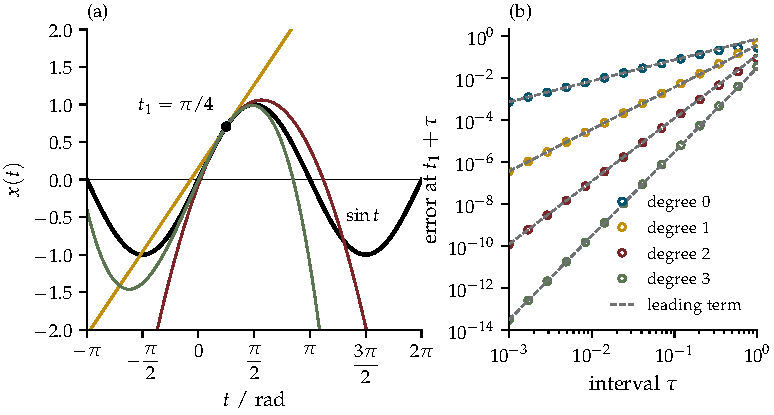
\includegraphics{ch01_motion/taylor}
\caption{Taylor polynomials of $x(t) = \sin t$ about $t_1 = \pi/4$. (a)
The polynomials of degrees 1, 2 and 3 (colours as in the key of b) follow
the function ever more closely near $t_1$. (b) The error of the polynomial
of degree $n$ at $t_1 + \tau$, including the constant polynomial of degree
0, with its leading term $\lvert x^{(n+1)}(t_1)\rvert\,\tau^{n+1}/(n+1)!$
(dashed); each error falls as $\tau^{n+1}$.}
\label{fig:mo-taylor}
\end{figure}

\subsection*{Two series used later}

Setting $t = 0$ in the Taylor series and writing $y$ for $\tau$, so that
$x(y) = x(0) + \dot{x}(0)\,y + \ddot{x}(0)\,y^2/2! + \dotsb$, and using
$\sin 0 = 0$ and $\cos 0 = 1$, the
derivatives of $\sin y$ at $y = 0$ are $0, 1, 0, -1, 0, 1, \dots$ and
those of $\cos y$ are $1, 0, -1, 0, 1, \dots$, so
\begin{equation}
   \sin y = y - \frac{y^3}{3!} + \frac{y^5}{5!} - \dotsb, \qquad
   \cos y = 1 - \frac{y^2}{2!} + \frac{y^4}{4!} - \dotsb .
   \label{eq:mo-sin-series}
\end{equation}
For small angles these give the approximations $\sin y \approx y$ and
$\cos y \approx 1 - y^2/2$, which are used throughout the book; the
first agrees with the limit $\sin h/h \to 1$ found in \cref{sec:mo-trig}.

\subsection*{Back to the ball}

For the ball, the Taylor series ends after its third term, because
$\dddot{x} = \dd a/\dd t = 0$ when the acceleration is constant, and
every higher derivative vanishes too. The expansion of
\cref{sec:mo-velocity},
\begin{equation*}
   x(t_1+\tau) = x(t_1) + \bigl(v_0 - g t_1\bigr)\,\tau - \tfrac12 g\,\tau^2 ,
\end{equation*}
was this series in disguise: its coefficients are $v(t_1)$ and
$\tfrac12 a$. For a general motion, the first three terms of
\cref{eq:mo-taylor} amount to \cref{eq:mo-constant} with the acceleration
held at its value at the start of the interval, and their error is of
order $\tau^3$, small when the interval is short. Advancing a motion
through many such intervals is how a computer follows it, and Chapter~9
develops this idea into the methods that molecular dynamics uses.

\notebook{01}{Taylor polynomials of growing order}

%=============================================================================!
% 1.9  FROM BALLS TO ATOMS                                                    !
%=============================================================================!
\section{From balls to atoms}
\label{sec:mo-atoms}

None of the preceding sections depended on the moving object being a
ball, and the same description applies directly to atoms. A system of $N$
atoms has a position vector for each atom, $\vb{r}_1(t), \dots,
\vb{r}_N(t)$, and each atom has its own velocity $\vb{v}_i =
\dd\vb{r}_i/\dd t$ and acceleration $\vb{a}_i = \dd\vb{v}_i/\dd t$. When
all the positions are collected into a single list of $3N$ numbers,
$\vb{r}^N = (\vb{r}_1, \dots, \vb{r}_N)$ (the superscript is a label,
not a power), the motion of the whole system becomes a single path
$\vb{r}^N(t)$: just as three numbers locate a point in space, $3N$
numbers locate a point in a space of $3N$ dimensions, which cannot be
drawn but obeys the same component-by-component rules, and every result of the preceding sections applies to each of its components.
The only change is in the units, which become \si{\angstrom},
\si{\femto\second}, \si{\angstrom\per\femto\second} and
\si{\angstrom\per\femto\second\squared}.

\subsection*{Velocities from frames}

A molecular dynamics calculation does not record this path continuously.
It stores frames instead, the positions of all the atoms at times
separated by an interval $\tau$, and the velocities must sometimes be
recovered from these frames afterwards. The derivative, a limit as $\tau
\to 0$, must then be replaced by a finite difference with $\tau$ fixed, and
the Taylor series of \cref{eq:mo-taylor} tells us how large an error this
introduces. We treat one coordinate $x$; every component of every atom
behaves in the same way.

The simplest choice is the forward difference, the secant slope of
\cref{sec:mo-velocity}. Subtracting $x(t)$ from both sides of
\cref{eq:mo-taylor} and dividing by $\tau$,
\begin{equation*}
   \frac{x(t+\tau) - x(t)}{\tau} = v(t) + \tfrac12 a(t)\,\tau
   + \order{\tau^2},
\end{equation*}
where the term $\tfrac16\dddot{x}\,\tau^2$ and the remainder, now
$\order{\tau^4}/\tau = \order{\tau^3}$, are both no larger than a constant
times $\tau^2$ when $\tau$ is small, and so together are $\order{\tau^2}$.
So the forward difference returns the velocity with an error whose leading
term, $\tfrac12 a\tau$, is proportional to $\tau$. For the ball this is
the term $-\tfrac12 g\tau$ of \cref{eq:mo-secant}.

A better estimate uses the frames on both sides of $t$. Writing the
Taylor series forwards and backwards in time, by replacing $\tau$ with
$-\tau$ in the second,
\begin{align*}
   x(t+\tau) &= x + v\tau + \tfrac12 a\tau^2 + \tfrac16\dddot{x}\tau^3
      + \tfrac1{24}x^{(4)}\tau^4 + \order{\tau^5},\\
   x(t-\tau) &= x - v\tau + \tfrac12 a\tau^2 - \tfrac16\dddot{x}\tau^3
      + \tfrac1{24}x^{(4)}\tau^4 + \order{\tau^5},
\end{align*}
where $x$, $v$, $a$, $\dddot{x}$ and $x^{(4)}$ are evaluated at $t$. The terms with
even powers of $\tau$ have the same sign in both lines, and those with odd
powers have opposite signs. Subtracting the second line from the first
therefore cancels the even terms and doubles the odd ones,
\begin{equation*}
   x(t+\tau) - x(t-\tau) = 2v\tau + \tfrac13\dddot{x}\,\tau^3
   + \order{\tau^5},
\end{equation*}
where the remainder is of order $\tau^5$ because the $\tau^4$ terms also
cancel. Dividing by $2\tau$ gives the central difference,
\begin{equation*}
   \frac{x(t+\tau) - x(t-\tau)}{2\tau} = v(t) + \tfrac16\,\dddot{x}(t)\,
   \tau^2 + \order{\tau^4},
\end{equation*}
whose error is proportional to $\tau^2$. Halving the interval therefore
halves the error of the forward difference but quarters that of the
central difference. In \texttt{mdlab} the central difference occupies a
single line.

\begin{code}
def central_difference(positions: ArrayLike, tau: float) -> NDArray:
    x = np.asarray(positions, dtype=float)
    return (x[2:] - x[:-2]) / (2.0 * tau)
\end{code}

Listings in this book are taken from \texttt{mdlab} without their
docstrings, which give the shape and unit of every argument. Python
counts from 0, so \texttt{x[2:]} holds the frames from the third onwards
and \texttt{x[:-2]} those up to the third from last; entry $k$ of their
difference is $x_{k+2} - x_k$, the central difference at frame $k + 1$,
so the first and last frames receive no velocity. \texttt{np.asarray}
turns the input into a NumPy array of decimal numbers, and the
annotations after the colons and the arrow only document the types
expected and returned.

\subsection*{A vibrating coordinate}

The atoms in molecules and solids vibrate (Chapter~4), and a vibrating
coordinate can be modelled by the sinusoid of \cref{sec:mo-trig} with zero
phase, $x(t) = A\sin\omega t$, of amplitude $A$, angular frequency $\omega$
and period $2\pi/\omega$. For this motion the central difference
can be evaluated exactly. Subtracting the two sine formulae of
\cref{eq:mo-addition},
\begin{align*}
   \sin(p+q) - \sin(p-q)
   &= (\sin p\cos q + \cos p\sin q) - (\sin p\cos q - \cos p\sin q)\\
   &= 2\cos p\sin q .
\end{align*}
With $p = \omega t$ and $q = \omega\tau$, and multiplying through by
$A/2\tau$,
\begin{equation}
   \frac{x(t+\tau) - x(t-\tau)}{2\tau}
   = \frac{A\cos\omega t\,\sin\omega\tau}{\tau}
   = \underbrace{A\omega\cos\omega t}_{v(t)}\;
     \frac{\sin\omega\tau}{\omega\tau} ,
   \label{eq:mo-sinc}
\end{equation}
where the last step multiplies and divides by $\omega$ so that the true
velocity $v(t) = A\omega\cos\omega t$ appears. Every recovered velocity is
therefore too small by the same factor, $\sin(\omega\tau)/(\omega\tau)$.
To see how close this factor is to 1, we divide the series for $\sin y$ in
\cref{eq:mo-sin-series} by $y$,
\begin{equation*}
   \frac{\sin y}{y} = 1 - \frac{y^2}{6} + \order{y^4} .
\end{equation*}
The relative error, the error divided by the true velocity, is therefore
\begin{equation*}
   \frac{v(t) - v(t)\sin(\omega\tau)/(\omega\tau)}{v(t)}
   = 1 - \frac{\sin\omega\tau}{\omega\tau} \approx \frac{(\omega\tau)^2}{6} .
\end{equation*}

For an amplitude of \SI{0.1}{\angstrom} and a period of
\SI{20}{\femto\second}, the angular frequency is $\omega =
2\pi/\SI{20}{\femto\second} = \SI{0.3142}{\per\femto\second}$. Frames
saved every \SI{1}{\femto\second} then give $\omega\tau = 0.3142$ and an
error of $0.3142^2/6 = \SI{1.645}{\percent}$ by the approximation, against
\SI{1.637}{\percent} exactly. Frames every \SI{0.1}{\femto\second} give
\SI{0.016}{\percent} either way, and frames every \SI{2}{\femto\second}
give \SI{6.58}{\percent} by the approximation against \SI{6.45}{\percent}
exactly (\cref{fig:mo-differences}). When $\tau$ equals half a
period, $\omega\tau = \pi$ and the factor $\sin\pi/\pi$ vanishes
altogether: $x(t+\tau)$ and $x(t-\tau)$ are then a whole period apart and
therefore equal, and the central difference detects no motion at all.

\begin{figure}[tb]
\centering
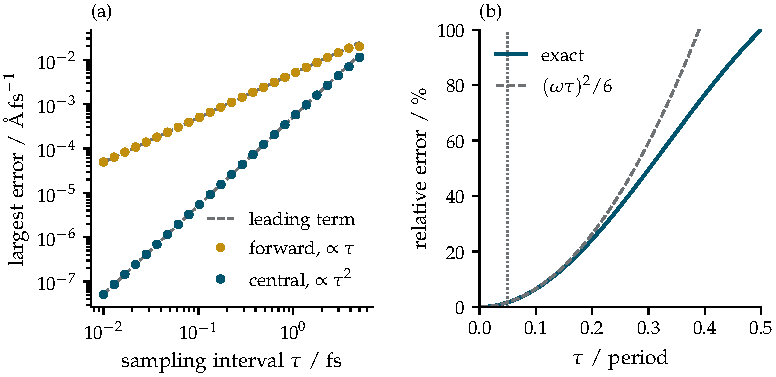
\includegraphics{ch01_motion/differences}
\caption{Velocities recovered from frames. A coordinate $x = A\sin\omega
t$ with $A = \SI{0.1}{\angstrom}$ and period $2\pi/\omega =
\SI{20}{\femto\second}$ is sampled every $\tau$. (a) Largest error of the
forward and central differences, with their leading terms
$A\omega^2\tau/2$ and $A\omega^3\tau^2/6$ (dashed). (b) Relative error of
the central difference, $1 - \sin(\omega\tau)/(\omega\tau)$, against its
leading term; the dotted line marks $\tau = \SI{1}{\femto\second}$.}
\label{fig:mo-differences}
\end{figure}

\begin{practice}
Frames must be closely spaced compared with the fastest motion that they
are intended to resolve, and \cref{eq:mo-sinc} makes this requirement
quantitative. The coordinates of real atoms move as sums of sinusoids of
several frequencies (Chapter~4). The central difference of a sum is the
sum of the central differences of its terms, so it shrinks the velocity
of each sinusoid by that sinusoid's own factor $\sin(\omega\tau)/
(\omega\tau)$. If the interval satisfies $(\omega_{\max}\tau)^2/6 \le
\epsilon$ for the highest angular frequency $\omega_{\max}$ present, each
sinusoid's velocity is recovered to a relative accuracy $\epsilon$, and
the error in the whole velocity is at most $\epsilon$ times the sum of
the largest speeds $A\omega$ of the sinusoids, since the size of a sum is
at most the sum of the sizes of its terms. This bounds the error
relative to the typical speed of the motion, not relative to the velocity
at each instant: where the sinusoids cancel and the velocity passes
through zero, even a small error is a large fraction of it. For $x =
\sin t - \tfrac12\sin 2t$, in metres with $t$ in seconds, and $\tau =
\SI{0.1}{\second}$, $(\omega_{\max}\tau)^2/6 = \SI{0.67}{\percent}$ with
$\omega_{\max} = 2$. The true velocity is $\cos t - \cos 2t$, while by
\cref{eq:mo-sinc} applied to each term the central difference is $\cos
t\,(\sin 0.1/0.1) - \cos 2t\,(\sin 0.2/0.2)$. At $t =
\SI{0.01}{\second}$, where the true velocity is
\SI{1.5e-4}{\metre\per\second}, the central difference gives
\SI{5.1e-3}{\metre\per\second}, 34 times too large. A path saved less
frequently than the criterion allows should store the velocities
directly. A related requirement limits the
size of the step that molecular dynamics itself can take (Chapter~9).
\end{practice}

\notebook{01}{sample an oscillation and recover its velocity}

%=============================================================================!
% 1.10  WHAT WE NOW HAVE                                                      !
%=============================================================================!
\unnumbered{What we now have}

Position, velocity and acceleration are successive derivatives with
respect to time, and a motion follows from its acceleration once the
initial position and velocity are known. The sine and cosine are the
coordinates of a point on the unit circle, and with angles measured in
radians their derivatives are $\cos$ and $-\sin$; and every sinusoid has an acceleration
proportional and opposite to its displacement. In two or three dimensions
position, velocity and acceleration are vectors; the velocity is always
directed along the path, whereas the acceleration may point in any
direction, and in uniform circular motion it points towards the centre.
The Taylor series approximates a motion over a short interval with an
error that falls as a known power of the interval. The same definitions
apply to a system of atoms, whose motion is a path in $3N$ dimensions,
and velocities recovered from saved frames carry an error determined by
the interval between the frames. What determines the acceleration has so
far been left open, and Chapter~2 answers that question by introducing
force.

%=============================================================================!
% 1.E  EXERCISES                                                              !
%=============================================================================!
\unnumbered{Exercises}
\label{sec:mo-exercises}

Full solutions are in \hyperref[sec:mo-solutions]{`Solutions to the
exercises'} at the end of the book, and Notebook~01 checks every
numerical answer.

\begin{exercise}[dimensions]
\label{ex:mo-dimensions}
Let $x$ be a height, $t$ a time, $v$ and $v_0$ velocities and $g$ an
acceleration. Which of the following equations balance in dimension?
(i)~$x = v_0 t^2$; (ii)~$v^2 = v_0^2 - 2gx$; (iii)~$t = \sqrt{2x/g}$;
(iv)~$x = v_0\,\mathrm{e}^{-gt}$.
\end{exercise}

\begin{exercise}[a higher throw]
\label{ex:mo-throw}
A ball is thrown vertically upwards at \SI{15}{\metre\per\second}. Find the
time it takes to reach the top, the greatest height it reaches and its
speed when it returns to the hand.
\end{exercise}

\begin{exercise}[displacement and distance]
\label{ex:mo-distance}
An object moves along a line with velocity $v(t) = 3t^2 - 12$, in metres
per second for $t$ in seconds. At what time $t \ge 0$ is it at rest, and
what is its acceleration at that instant? Find its displacement between $t
= 0$ and $t = \SI{3}{\second}$, and the total distance it travels over the
same interval, $\int\lvert v\rvert\,\dd t$.
\end{exercise}

\begin{exercise}[radians]
\label{ex:mo-radians}
Express \SI{1.1}{\radian} in degrees and \ang{135} in radians, and find
the length of the arc cut off by an angle of \ang{135} on a wheel of
radius \SI{0.35}{\metre}.
\end{exercise}

\begin{exercise}[an identity]
\label{ex:mo-identity}
Starting from the double-angle formula $\cos 2\theta = \cos^2\theta -
\sin^2\theta$ and $\cos^2\theta + \sin^2\theta = 1$, show that $\sin^2
\theta = \tfrac12(1 - \cos2\theta)$. Use it to find $\sin(\pi/8)$ exactly,
and give its value to four decimal places.
\end{exercise}

\begin{exercise}[a sinusoid]
\label{ex:mo-sinusoid}
A coordinate moves as $x(t) = 0.2\sin(5t + \pi/6)$, in metres for $t$ in
seconds. Find its amplitude, period and frequency, its largest speed and
largest acceleration, and the first time after $t = 0$ at which $x$ is
greatest.
\end{exercise}

\begin{exercise}[range]
\label{ex:mo-range}
Show that the range $d = v_0^2\sin2\alpha/g$ is greatest when $\alpha =
\ang{45}$. For $v_0 = \SI{12}{\metre\per\second}$, find the two launch
angles that give a range of \SI{10}{\metre}.
\end{exercise}

\begin{exercise}[an orbit]
\label{ex:mo-orbit}
A point moves anticlockwise around a circle of radius \SI{1.0}{\angstrom}
at a constant speed of \SI{0.02}{\angstrom\per\femto\second}. Find the
magnitude of its acceleration and its period.
\end{exercise}

\begin{exercise}[a Taylor estimate]
\label{ex:mo-taylor}
Use the series of \cref{eq:mo-sin-series} to approximate $\cos 0.1$ by
its terms up to $y^2$. Estimate the error from the first term omitted,
and compare with the exact value.
\end{exercise}

\begin{exercise}[sampling]
\label{ex:mo-sampling}
Show that for $x = A\sin\omega t$ the largest error of the forward
difference, relative to the largest speed $A\omega$, is approximately
$\omega\tau/2$ when $\omega\tau$ is small. For a coordinate with a period
of \SI{20}{\femto\second}, find the largest frame interval $\tau$ for which
velocities recovered by central differences are within \SI{1}{\percent}.
\end{exercise}


%=============================================================================!
% CHAPTER 2  FORCES AND NEWTON'S LAWS                                         !
%=============================================================================!
\chapter{Forces and Newton's laws}
\label{ch:newton}

%=============================================================================!
% 2.0  CHAPTER OPENING                                                        !
%=============================================================================!
Chapter~1 described motion through position, velocity and acceleration.
Once the acceleration is known at every instant, the starting position
and velocity fix the motion, but we have yet to establish what determines
that acceleration. Newton's laws connect it to the pushes and pulls on a
body, meaning the object whose motion we follow. We first treat the body
as a particle: a point that carries its mass, so that we can study its
motion from place to place before considering rotation in Chapter~5.

To use those pushes and pulls in a calculation, we need to measure them
as forces and establish the frames of reference in which the laws hold.
We then introduce mass and apply the laws to a falling ball, a bead sinking
through a thick liquid and a block on a spring. When several bodies
interact, adding their equations reveals a conserved quantity, the total
momentum, provided that the external forces sum to zero. The same
calculation gives the equations of molecular dynamics for a collection of
atoms. Chapter~3 develops a further consequence of these equations: the
conditions under which the total energy is conserved.

%=============================================================================!
% 2.1  FORCE AND THE FIRST LAW                                                !
%=============================================================================!
\section{Force and the first law}
\label{sec:ne-force}

In everyday speech a force is a push or a pull: a hand pushing a door, a
rope pulling a sledge, a magnet pulling a pin. To build a law of motion on
forces we first need to measure them, and this section shows how, before
stating the first of Newton's three laws.

\subsection*{Measuring a force}

A spring stretches when it is pulled, and the harder the pull, the further
it stretches. A spring with a scale beside it, called a spring balance,
therefore turns a pull into a reading. We can define a unit of force as
the pull that stretches one particular standard spring by one particular
amount. Two identical standard springs pulling side by side, each
stretched by that amount, then exert two units, three springs exert three
units, and so on (\cref{fig:ne-force}a). In this way a force acquires a
size, a number of units. \Cref{sec:ne-second} replaces this home-made
unit by the
standard one, the newton.

A force also has a direction, the direction in which it pulls, so it is a
vector. When several forces act on one body together, experiment shows
that their combined effect on its motion from place to place is that of a
single force equal to their vector sum, called the net force,
\begin{equation*}
   \vb{F} = \vb{F}_1 + \vb{F}_2 + \dotsb ,
\end{equation*}
in the sense in which a net profit is what remains when everything is
added up. A pull of 4 units towards the east and a pull of 3 units towards
the north, for example, are the vectors $(4, 0)$ and $(0, 3)$ when the
$x$ axis points east and the $y$ axis north. Adding component by
component (\cref{sec:mo-plane}) gives $(4, 3)$. This is the same as
drawing the second arrow from the tip of the first, since starting at the
tip of $(4, 0)$ and moving by $(0, 3)$ ends at $(4, 3)$
(\cref{fig:ne-force}b). The two pulls therefore act like a single pull of
length $(4^2 + 3^2)^{1/2} = 5$ units, by Pythagoras' theorem, directed at
an angle $\theta$ north of east. Writing $(4, 3) = 5(\cos\theta,
\sin\theta)$ gives $\tan\theta = \sin\theta/\cos\theta = 3/4$. The tangent can be
undone as the sine was in \cref{sec:mo-trig}: for any number $s$,
$\arctan s$ is the angle between $-\pi/2$ and $\pi/2$ whose tangent is
$s$, and here $\theta = \arctan(3/4) = \SI{0.644}{\radian}$, or
\ang{36.9}. Two forces of equal size pulling
in opposite directions add to zero, so a body can be pushed and pulled by
several forces while the net force on it vanishes. Such a body may
still turn: two equal and opposite pushes at opposite corners of a book
lying on a table add to zero, yet set the book spinning, because where a
force acts decides how it turns a body. Turning is the subject of
Chapter~5, and until then every body is a particle, for which only the
net force matters.

\begin{figure}[htb]
\centering
\begin{tikzpicture}[line cap=round, line join=round,
   force/.style={-{Stealth[length=5pt]}, line width=1.1pt},
   coil/.style={decorate, decoration={coil, aspect=0.45,
      segment length=3pt, amplitude=3pt, pre length=3pt,
      post length=3pt}, line width=0.6pt}]
   % (a) one spring, then two side by side, each stretched by one unit
   \begin{scope}
      \node[anchor=west] at (-0.4,1.75) {\small (a)};
      \fill[black!35] (-0.25,1.45) rectangle (2.95,1.55);
      \draw[coil] (0.3,1.45) -- (0.3,0.35);
      \draw[black!40] (0.0,0.35) -- (0.0,1.25);
      \foreach \y in {0.35,0.65,0.95,1.25}
         \draw[black!40] (0.0,\y) -- (0.08,\y);
      \draw[force] (0.3,0.35) -- (0.3,-0.35);
      \node[below] at (0.3,-0.38) {\small 1 unit};
      \draw[coil] (1.9,1.45) -- (1.9,0.35);
      \draw[coil] (2.4,1.45) -- (2.4,0.35);
      \draw[line width=0.8pt] (1.8,0.35) -- (2.5,0.35);
      \draw[force] (2.15,0.35) -- (2.15,-1.05);
      \node[below] at (2.15,-1.08) {\small 2 units};
   \end{scope}
   % (b) two forces added tip to tail
   \begin{scope}[xshift=5.0cm, yshift=-0.9cm, scale=0.62]
      \node[anchor=west] at (-0.6,4.1) {\small (b)};
      \draw[force] (0,0) -- (4,0) node[midway, below] {\small 4 east};
      \draw[force] (4,0) -- (4,3) node[midway, right] {\small 3 north};
      \draw[force, accent] (0,0) -- (4,3)
         node[midway, above left] {\small net force, 5};
      \draw[black!50, line width=0.4pt] (1.0,0) arc[start angle=0,
         end angle=36.87, radius=1.0];
      \node at (1.45,0.42) {\small \ang{36.9}};
      \fill (0,0) circle (1.5pt);
   \end{scope}
\end{tikzpicture}
\caption{Measuring and adding forces. (a) A unit of force stretches a
standard spring by a set amount; two such springs pulling together exert
two units. (b) Pulls of 4 units east and 3 units north, drawn tip to tail,
add to a net force of 5 units at \ang{36.9} north of east.}
\label{fig:ne-force}
\end{figure}

\subsection*{The first law}

A book slid across a table slows down and stops. The table and the air
exert forces on it: friction, the grip of one surface sliding over
another, and drag, the resistance of the air or liquid a body moves
through. Where these forces are made small, the book's behaviour changes.
On smooth ice, or on an air-hockey table, where a cushion of air lifts the
puck clear of the surface, a puck glides on at nearly constant speed in a
straight line. We call a surface smooth when the friction it exerts is
small enough to neglect.

Since forces acting together behave like their net force, a body whose
forces add to zero moves as one with no force on it at all. Newton's
first law states the result: a body on which no net force acts keeps moving in a straight line at constant
speed, that is, at constant velocity, and a body at rest stays at rest. A
force is therefore not needed to keep a body moving, only to change its
motion. The next section shows that this law cannot be true for every
observer, and uses that fact to pick out the viewpoints from which all
three laws hold.

\begin{selfcheck}
A puck glides across smooth ice in a straight line at a steady
\SI{3}{\metre\per\second}. What is the net force on it?
\end{selfcheck}

%=============================================================================!
% 2.2  FRAMES OF REFERENCE                                                    !
%=============================================================================!
\section{Frames of reference}
\label{sec:ne-frames}

Every position in Chapter~1 was measured from some origin, along some
axes, with times read from some clock. That choice is called a frame of
reference. \Cref{sec:mo-atoms} used the word frame for a saved snapshot
of positions, so here we always say frame of reference in full. Two
observers moving relative to each other use different frames of
reference and describe the same motion differently. This section works
out how their descriptions are related, which tells us from which frames
of reference the first law can hold.

\subsection*{One throw seen from two frames of reference}

A train runs along a straight, level track at a constant velocity
$\vb{u}$. We take the $x$ axis along the track in the direction of travel
and the $y$ axis vertically upwards, so that $\vb{u} = (5,
0)$\,\si{\metre\per\second}. A passenger throws a ball straight up, as
the passenger sees it, at \SI{6}{\metre\per\second}. To the passenger the
ball rises and falls along a vertical line and lands back in the hand
(\cref{fig:ne-frames}a). Someone standing on the platform sees the same
ball travel forwards with the train while it rises and falls, and so
trace out a parabola (\cref{fig:ne-frames}b). Both descriptions are
correct; they differ because they are made from different frames of
reference.

\begin{figure}[tb]
\centering
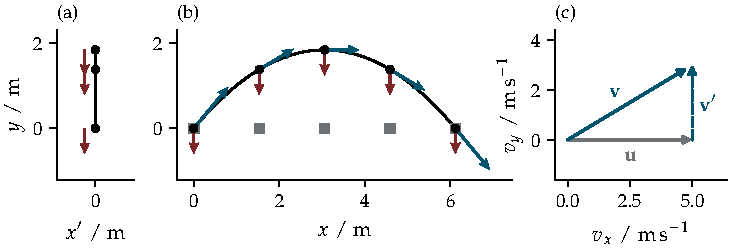
\includegraphics{ch02_newton/frames}
\caption{A ball thrown straight up at \SI{6}{\metre\per\second} by a
passenger in a train moving at $\vb{u} = (5, 0)$\,\si{\metre\per\second},
at five equally spaced times from the throw to the catch
\SI{1.224}{\second} later. (a) In the frame of reference of the train
the ball moves on a vertical line; it passes the same heights on the way
up and down, so the five positions show as three. Arrows give its
acceleration. (b) In the frame of reference of the platform it follows a
parabola, with velocity (teal) and acceleration (dark red); squares mark
the passenger's hand. (c) The velocities at the second instant, $t = 1.224/4 =
\SI{0.306}{\second}$, when the passenger sees the ball rising at $6 -
9.80665\times0.306 = \SI{3}{\metre\per\second}$: the platform sees $\vb{v}$, which is the velocity
$\vb{v}' = (0, 3)$\,\si{\metre\per\second} seen in the train plus the
velocity $\vb{u}$ of the train.}
\label{fig:ne-frames}
\end{figure}

To relate the two descriptions, the platform observer measures positions
from a fixed mark on the platform, the passenger measures them from the
hand, and both sets of axes point the same way. The hand moves at the
constant velocity $\vb{u}$, so by \cref{eq:mo-constant} with zero
acceleration it is at $\vb{r}_0 + \vb{u}t$ at time $t$, where $\vb{r}_0$
is its position at $t = 0$. To go from the mark to the ball we can go
first from the mark to the hand and then from the hand to the ball
(\cref{fig:ne-positions}), and adding these two vectors gives the
position $\vb{r}$ of the ball seen from the platform in terms of its
position $\vb{r}'$ seen from the hand,
\begin{equation*}
   \vb{r} = \vb{r}_0 + \vb{u}t + \vb{r}' .
\end{equation*}
Subtracting $\vb{r}_0 + \vb{u}t$ from both sides gives the position seen
in the train,
\begin{equation}
   \vb{r}' = \vb{r} - \vb{r}_0 - \vb{u}t .
   \label{eq:ne-galilean}
\end{equation}
Here we have assumed that both observers read the same time $t$ from
their clocks, which is true to an excellent approximation for every speed
far below that of light, about \SI{3e8}{\metre\per\second}, and so for
everything in this book.

\begin{figure}[htb]
\centering
\begin{tikzpicture}[scale=1.15, line cap=round,
   vec/.style={-{Stealth[length=5pt]}, line width=0.9pt}]
   \coordinate (O) at (0,0);
   \coordinate (H) at (3.2,0.35);
   \coordinate (B) at (3.9,2.0);
   \draw[vec] (O) -- (H) node[midway, below] {\small $\vb{r}_0 + \vb{u}t$};
   \draw[vec] (H) -- (B) node[midway, right] {\small $\vb{r}'$};
   \draw[vec, accent] (O) -- (B) node[midway, above left] {\small $\vb{r}$};
   \fill (O) circle (1.6pt) node[below left] {\small mark on the platform};
   \fill (H) circle (1.6pt) node[below right] {\small hand};
   \fill[accent] (B) circle (2pt) node[above right] {\small ball};
\end{tikzpicture}
\caption{The position $\vb{r}$ of the ball seen from the platform is the
position $\vb{r}_0 + \vb{u}t$ of the hand plus the position $\vb{r}'$ of
the ball seen from the hand.}
\label{fig:ne-positions}
\end{figure}

\subsection*{Velocities and accelerations}

Differentiating \cref{eq:ne-galilean} with respect to time relates the
velocities. The starting point $\vb{r}_0$ is fixed, so its derivative is
zero, and the derivative of $\vb{u}t$ is $\vb{u}$ because $\vb{u}$ is
constant:
\begin{align*}
   \frac{\dd\vb{r}'}{\dd t}
   &= \frac{\dd\vb{r}}{\dd t} - \frac{\dd\vb{r}_0}{\dd t}
      - \frac{\dd(\vb{u}t)}{\dd t}
      && \text{differentiating each term}\\
   &= \vb{v} - \vb{0} - \vb{u}
      && \text{$\vb{r}_0$ fixed, $\vb{u}$ constant,}
\end{align*}
so that
\begin{equation}
   \vb{v}' = \vb{v} - \vb{u} .
   \label{eq:ne-velocity-frames}
\end{equation}
The velocity seen in the train is the velocity seen from the platform,
less the velocity of the train. Differentiating once more, $\vb{u}$ is
constant and drops out entirely, and the two observers find the same
acceleration,
\begin{equation*}
   \vb{a}' = \vb{a} .
\end{equation*}

For the throw, the passenger sees the ball leave the hand with velocity
$\vb{v}' = (0, 6)$\,\si{\metre\per\second}, so the platform sees it leave
with $\vb{v} = \vb{v}' + \vb{u} = (5, 6)$\,\si{\metre\per\second}, a
speed of $(5^2 + 6^2)^{1/2} = \SI{7.810}{\metre\per\second}$.
\Cref{fig:ne-frames}(c) draws this sum at a later instant. Both observers
see the same acceleration, $(0, -g)$, and, because $\vb{u}$ has no
vertical component, the same vertical starting velocity,
\SI{6}{\metre\per\second}, so they see the same vertical motion. By
\cref{eq:mo-constant,eq:mo-v2}, the ball rises for $6/g =
\SI{0.612}{\second}$ to a greatest height of $6^2/2g = \SI{1.835}{\metre}$
and falls back in the same time, landing after \SI{1.224}{\second}. In
that time the platform observer sees it travel $5\times1.224 =
\SI{6.12}{\metre}$ along the track, which is exactly how far the hand has
moved, so the passenger catches it.

\subsection*{Inertial frames of reference}

Positions and velocities depend on the frame of reference, but
accelerations do not, for any two frames of reference moving at constant
velocity relative to each other. The agreement fails when one of them
accelerates. If the train brakes, the hand no longer moves at constant
velocity. We write its position as some function $\vb{s}(t)$, which for
the steady train was $\vb{r}_0 + \vb{u}t$. The same subtraction then
gives $\vb{r}' = \vb{r} - \vb{s}(t)$, and differentiating twice,
\begin{equation*}
   \vb{a}' = \vb{a} - \frac{\dd^2\vb{s}}{\dd t^2} .
\end{equation*}
The two observers now disagree about accelerations, by exactly the
acceleration of the train. Picture a cup on a smooth table in the train.
If the train slows at \SI{2}{\metre\per\second\squared}, its acceleration
is $\dd^2\vb{s}/\dd t^2 = (-2, 0)$\,\si{\metre\per\second\squared},
pointing backwards. Nothing pushes the cup along the track, so from the
platform $\vb{a} = \vb{0}$, and the passenger sees $\vb{a}' = \vb{0} -
(-2, 0) = (2, 0)$\,\si{\metre\per\second\squared}: the cup slides
forwards with nothing pushing it, which breaks the first law, while from the platform it simply
keeps moving at its old velocity as the train slows beneath it, as the
first law says.

The first law therefore cannot hold in every frame of reference, and we
turn this round into a definition. A frame of reference in which a body
with no net force on it moves at constant velocity is called inertial,
from inertia, the tendency of a body to keep the velocity it has. What
experiment adds is that such frames of reference exist. A frame of
reference fixed to the ground is very nearly inertial. The Earth turns
once in \SI{86164}{\second} measured against the distant stars. This is
a little less than the \SI{86400}{\second} of a 24-hour day, which is
measured against the Sun: the Earth's yearly journey round the Sun adds
one turn against the stars each year, so $86400\times365.24/366.24 =
\SI{86164}{\second}$. Its angular speed is therefore $\omega = 2\pi/86164
= \SI{7.29e-5}{\radian\per\second}$. In a frame of reference with its
origin at the Earth's centre and its axes pointing at fixed distant
stars, a point on the equator, carried round a circle of radius $R =
\SI{6.38e6}{\metre}$, has by \cref{eq:mo-circle} an acceleration of only
$\omega^2 R = (7.29\times10^{-5})^2\times6.38\times10^6 =
\SI{0.034}{\metre\per\second\squared}$, about \SI{0.35}{\percent} of
$g$. By $\vb{a}' = \vb{a} - \dd^2\vb{s}/\dd t^2$, a body with no net
force on it therefore seems, from the ground, to accelerate by at most
about this much; the turning of the ground's axes adds effects that are
smaller still at everyday speeds.
Since accelerations agree between frames of reference moving at constant
velocity relative to each other, every frame of reference moving at
constant velocity relative to the ground is very nearly inertial as well. All three
of Newton's laws are stated for inertial frames of reference, and from
here on every motion is described in one.

\notebook{02}{change the train's speed and watch both views of the throw}

\begin{selfcheck}
A passenger walks towards the back of the train at \SI{1}{\metre\per\second}
while the train moves forwards at \SI{5}{\metre\per\second}. What is the
passenger's velocity seen from the platform? Is a spinning roundabout an
inertial frame of reference?
\end{selfcheck}

%=============================================================================!
% 2.3  MASS AND THE SECOND LAW                                                !
%=============================================================================!
\section{Mass and the second law}
\label{sec:ne-second}

The first law says what happens when no net force acts. The second says
what a net force does, and to state it we need one more quantity, mass,
which measures how strongly a body resists being accelerated.

\subsection*{Mass}

Pull two different bodies on a smooth level floor with the same force, for instance by stretching
the same spring by the same amount, and they accelerate differently: a
loaded trolley gathers speed more slowly than an empty one. Experiment
shows that the ratio of their accelerations, $a_2/a_1$, does not depend on
which force is used. Because the ratio does not depend on the force, it
belongs to the two bodies alone, and we can use it to give each body a
number, its mass, by defining the ratio of their masses as
\begin{equation*}
   \frac{m_1}{m_2} = \frac{a_2}{a_1} .
\end{equation*}
The body that accelerates less has the larger mass. If, under the same
pull, an empty trolley accelerates at \SI{3}{\metre\per\second\squared}
and a loaded one at \SI{1}{\metre\per\second\squared}, the loaded trolley
has three times the mass of the empty one. Choosing one body as a
standard, the kilogram (\si{\kilogram}), then fixes every other mass. Mass
is a new kind of quantity alongside length and time, and we give it the
dimension $\mathsf{M}$. It measures the inertia of the body, and
experiment also shows that when two bodies are joined their masses add.

\subsection*{The second law}

Two experiments now combine into a law. The mass
experiment says that one force gives two bodies accelerations in the
inverse ratio of their masses, $a_2/a_1 = m_1/m_2$, so the product $m_1
a_1 = m_2 a_2$ is the same for both bodies: it depends on the force and
not on the body it acts on. Experiment also shows that $n$ standard
springs pulling together give a body $n$ times the acceleration that one
gives it, so the product is $n$ times as large when the force is $n$
units. The product of mass and acceleration is therefore proportional to
the force, $F = c\,ma$
for some constant $c$, and the acceleration points along the force. We
are free to choose the unit of force, and choosing it to make $c = 1$, as
the newton below does, gives Newton's second law,
\begin{equation}
   \vb{F} = m\vb{a} ,
   \label{eq:ne-second-law}
\end{equation}
where $\vb{F}$ is the net force on the body. Because it is a vector
equation, it holds for each component separately: $F_x = m a_x$, $F_y =
m a_y$ and $F_z = m a_z$.

The law also fixes the unit of force. One newton (\si{\newton}) is the
force that gives one kilogram an acceleration of one metre per second per
second, $\SI{1}{\newton} = \SI{1}{\kilogram\metre\per\second\squared}$,
so force has dimension $\mathsf{M}\mathsf{L}\mathsf{T}^{-2}$. The spring
unit of \cref{sec:ne-force} was a stopgap: from now on forces are measured
in newtons, and spring balances are marked in newtons. A trolley of
\SI{20}{\kilogram} pushed with a net force of \SI{10}{\newton}
accelerates at $10/20 = \SI{0.5}{\metre\per\second\squared}$, in the
direction of the push.

\begin{keyidea}
In an inertial frame of reference the net force on a body equals its mass
times its acceleration, $\vb{F} = m\vb{a}$, where the net force is the
vector sum of every force acting on the body.
\end{keyidea}

\begin{selfcheck}
A net force of \SI{6}{\newton} acts on a \SI{2}{\kilogram} body. What is
its acceleration? What would it be if the mass were doubled?
\end{selfcheck}

%=============================================================================!
% 2.4  THE THIRD LAW                                                          !
%=============================================================================!
\section{The third law}
\label{sec:ne-third}

Forces do not appear from nowhere: every force on a body is exerted by
some other body. The third law describes what happens at the other end,
and it is what later lets us treat several bodies, and many atoms,
together.

We write $\vb{F}_{AB}$ for the force on body $A$ exerted by body $B$; the
first subscript names the body that feels the force. The third law states
that forces between two bodies come in matched pairs,
\begin{equation*}
   \vb{F}_{AB} = -\vb{F}_{BA} ,
\end{equation*}
equal in size and opposite in direction. Like the second law, this is a
fact of experiment: hook two spring balances together and pull them apart,
and they always show the same reading, however hard or unevenly you pull.
When you push on a wall, the wall pushes back on you with an equal force.
When the Earth pulls a falling ball down, the ball pulls the Earth up with
a force of the same size. A ball of half a kilogram falls, with air
resistance negligible, at the acceleration $g$ of Chapter~1, so by the
second law the Earth's pull on it is $0.5\times9.80665 =
\SI{4.9}{\newton}$, its weight (\cref{sec:ne-gravity}). The Earth's mass
is about \SI{6e24}{\kilogram}, so by the second law again the Earth's
acceleration is
$4.9/(6\times10^{24}) = \SI{8e-25}{\metre\per\second\squared}$, far too
small to notice.

The two forces of a pair always act on different bodies, so they never
cancel in the second law of either body. A book resting on a table shows
the commonest confusion (\cref{fig:ne-third}). The Earth pulls the book
down and the table pushes it up, and these two forces are equal and
opposite, but they are not a third-law pair: both act on the book, and
they are equal only because the book does not accelerate. The partner of
the Earth's pull on the book is the book's pull on the Earth, and the
partner of the table's push on the book is the book's push on the table.

\begin{figure}[htb]
\centering
\begin{tikzpicture}[line cap=round,
   force/.style={-{Stealth[length=5pt]}, line width=1.1pt},
   body/.style={line width=0.6pt, fill=black!8}]
   % the book, the table and the Earth, drawn apart
   \draw[body] (-0.6,2.6) rectangle (0.6,3.1);
   \draw[body] (-2.9,1.2) rectangle (2.9,1.34);
   \draw[line width=0.6pt] (-2.7,1.2) -- (-2.7,0.3) (2.7,1.2) -- (2.7,0.3);
   \fill[black!10] (-3.2,-1.6) arc[start angle=140, end angle=40,
      radius=4.18] -- cycle;
   \node at (0,-1.25) {\small Earth};
   \node at (1.05,2.85) {\small book};
   \node[right] at (2.9,1.27) {\small table};
   % one pair: the table pushes the book up, the book pushes the table down
   \draw[force] (-0.25,3.1) -- (-0.25,3.9)
      node[midway, left] {\small table on book};
   \draw[force] (-0.25,1.34) -- (-0.25,0.4)
      node[midway, left] {\small book on table};
   % the other pair: the Earth pulls the book, the book pulls the Earth
   \draw[force, accent] (0.25,2.6) -- (0.25,1.8)
      node[midway, right] {\small Earth on book};
   \draw[force, accent] (0.25,-0.1) -- (0.25,0.7)
      node[midway, right] {\small book on Earth};
\end{tikzpicture}
\caption{The forces between a book resting on a table, the table and the
Earth, with the three bodies drawn apart for clarity. The black arrows
are one third-law pair, the table's push on the book and the book's push
on the table; the teal arrows are another, the Earth's pull on the book
and the book's pull on the Earth. The two forces on the book itself, one
from each pair, balance because the book does not accelerate. Forces
between the table and the Earth are not drawn.}
\label{fig:ne-third}
\end{figure}

\begin{selfcheck}
The Earth pulls an apple down and the apple pulls the Earth up with an
equal force. Why does the apple fall towards the Earth, rather than the
Earth towards the apple?
\end{selfcheck}

%=============================================================================!
% 2.5  WEIGHT, FREE FALL AND FREE-BODY DIAGRAMS                               !
%=============================================================================!
\section{Weight, free fall and free-body diagrams}
\label{sec:ne-gravity}

With the second law in hand we can explain the first motion of
Chapter~1, the thrown ball, which was there described without a cause.

\subsection*{Weight}

Near the surface of the Earth every body is pulled downwards by a force,
its weight. Hanging a body at rest from a spring balance measures its
weight: the body does not accelerate, so by the second law the balance's
upward pull equals the Earth's downward pull (the lamp below works this
through). Such measurements show that the weight is proportional to the
mass: twice, three times or half the mass gives twice, three times or
half the reading. We therefore write the weight as $m\vb{g}$, where $\vb{g}$ is a vector
pointing straight down whose length $g$ is the same for every body. Since
weight divided by mass is in newtons per kilogram, which by the definition
of the newton is \si{\metre\per\second\squared}, $g$ has the units of an
acceleration. Its standard value is $g = \SI{9.80665}{\metre\per\second
\squared}$, and the free-fall argument below shows that it is the $g$ of
Chapter~1. An apple of \SI{100}{\gram} weighs $0.1\times
9.80665 = \SI{0.981}{\newton}$, about one newton.

In everyday speech weight often means mass, as in `a bag of flour weighs
a kilogram'. This book keeps them apart. Mass, in kilograms, measures
inertia and is the same everywhere; weight, in newtons, is the pull of the
Earth, and on the Moon, whose pull is weaker, the same bag would weigh
about a sixth as much. A kitchen scale measures the force and divides by
$g$ to display a mass.

\subsection*{Free fall}

A ball in flight, with air resistance negligible, feels its weight and
nothing else, a motion called free fall. The second law gives $m\vb{a} =
m\vb{g}$, and dividing both sides by $m$,
\begin{equation*}
   \vb{a} = \vb{g} .
\end{equation*}
The mass cancels, so every body falls with the same acceleration, whatever
its mass. This is why $g$ in Chapter~1 was the same for every object, and
it rests on the experimental fact that weight is proportional to mass. A
feather and a coin dropped together in a room do not land together, but
only because the drag of the air (\cref{sec:ne-drag}) is large compared
with the feather's tiny weight. Without air they fall together, as an
astronaut showed on the Moon in 1971 by dropping a hammer and a feather
side by side.

We can now derive the motion of the ball that Chapter~1 took from
observation. The motion is along a single vertical line, so, as in
\cref{eq:mo-ball}, we call the height $x$ and measure it upwards. The
component of $\vb{a} = \vb{g}$ along this line is
\begin{equation*}
   \frac{\dd^2 x}{\dd t^2} = -g ,
\end{equation*}
the minus sign because $\vb{g}$ points down. Integrating once from $t =
0$, as in \cref{sec:mo-integrating}, gives $\dd x/\dd t = v_0 - gt$, where
$v_0$ is the launch velocity. Integrating again, with the ball leaving the
hand at $x = 0$, gives
\begin{equation*}
   x(t) = v_0 t - \tfrac12 g t^2 ,
\end{equation*}
which is \cref{eq:mo-ball}. The projectile follows in the same way: the
horizontal component of $\vb{g}$ is zero, so the horizontal velocity
stays constant.

For atoms, gravity hardly matters: \cref{sec:ne-atoms} shows that the
weight of an atom is some $10^{16}$ times smaller than the forces its
neighbours exert on it.

\subsection*{Free-body diagrams}

Applying the second law to a body starts with a free-body diagram: a
sketch of the body alone, with an arrow for every force acting on it and
for nothing else. \Cref{fig:ne-free-body}(a) shows the ball in flight,
which feels only its weight; its velocity is drawn dashed, because a
velocity is not a force. \Cref{fig:ne-free-body}(b) shows a lamp of
\SI{2}{\kilogram} hanging at rest from a cord. Two forces act on it: its
weight, $mg$ downwards, and the pull of the cord, called its tension,
upwards, which we write $F_{\mathrm{cord}}$. The lamp does not accelerate,
so by the second law the net force on it is zero, and taking upwards as
positive,
\begin{equation*}
   F_{\mathrm{cord}} - mg = 0
   \quad\Longrightarrow\quad
   F_{\mathrm{cord}} = mg = 2\times9.80665\ \si{\newton}
   = \SI{19.6}{\newton} .
\end{equation*}
The arrows of a free-body diagram are labelled with the sizes of the
forces, and their directions are shown by the arrows themselves.

\begin{figure}[htb]
\centering
\begin{tikzpicture}[scale=1.25, line cap=round,
   force/.style={-{Stealth[length=6pt]}, line width=1.2pt},
   body/.style={line width=0.6pt, fill=black!8}]
   % (a) the ball in flight
   \begin{scope}
      \node at (-1.3,1.55) {\small (a)};
      \draw[body] (0,0) circle (0.3);
      \draw[accent, -{Stealth[length=5pt]}, dashed, line width=0.8pt]
         (0.3,0.17) -- (1.0,0.85) node[right] {\small $\vb{v}$};
      \draw[force] (0,0) -- (0,-1.25) node[right] {\small $mg$};
      \fill (0,0) circle (1.4pt);
      \node at (0,-1.75) {\small ball in flight};
   \end{scope}
   % (b) the lamp hanging at rest from a cord
   \begin{scope}[xshift=4.0cm]
      \node at (-1.3,1.55) {\small (b)};
      \fill[black!35] (-0.6,1.45) rectangle (0.6,1.55);
      \draw[line width=0.8pt] (0,1.45) -- (0,0.3);
      \draw[body] (-0.35,0.3) -- (0.35,0.3) -- (0.5,-0.2) -- (-0.5,-0.2)
         -- cycle;
      \draw[force] (0,0.05) -- (0,1.2)
         node[midway, right=2pt] {\small $F_{\mathrm{cord}}$};
      \draw[force] (0,0.05) -- (0,-1.25) node[right] {\small $mg$};
      \fill (0,0.05) circle (1.4pt);
      \node at (0,-1.75) {\small hanging lamp};
   \end{scope}
\end{tikzpicture}
\caption{Free-body diagrams. (a) A ball in flight feels only its weight;
its velocity is dashed, because it is not a force. (b) A lamp hanging at
rest feels its weight and the tension $F_{\mathrm{cord}}$ of the cord,
which balance.}
\label{fig:ne-free-body}
\end{figure}

\begin{selfcheck}
A hammer and a feather are dropped together, first in a vacuum, then in
air. Which lands first in each case, and why?
\end{selfcheck}

%=============================================================================!
% 2.6  EQUATIONS OF MOTION AND THE STATE                                      !
%=============================================================================!
\section{Equations of motion and the state}
\label{sec:ne-equations}

For the falling ball the force was constant, and two integrations gave
the motion. Most forces are not constant: the drag of a liquid grows with
the speed of the body moving through it, and the pull of a spring grows
with how far it is stretched. This section shows what the second law
becomes in general, and what must be known at one instant to predict the
whole motion.

\subsection*{The equation of motion}

For motion along a line the force may depend on the position $x$, on the
velocity $v$ and on the time $t$, and we write it $F(x, v, t)$. Since the
acceleration is the second derivative of the position, the second law
reads
\begin{equation}
   m\,\frac{\dd^2 x}{\dd t^2} = F(x, v, t) .
   \label{eq:ne-eom}
\end{equation}
An ordinary equation such as $x^2 = 4$ has numbers as its unknowns;
\cref{eq:ne-eom} has a whole function, $x(t)$, as its unknown, and it
contains that function through its derivatives. An equation of this kind
is called a differential equation. Its order is that of the highest
derivative it contains, so \cref{eq:ne-eom} is of second order. It is the
equation of motion of the body, and solving it means finding a function
$x(t)$ for which it holds at every instant.

\subsection*{The state}

\Cref{eq:ne-eom} can be split into two first-order equations by treating
the velocity as a second unknown. The velocity is the rate of change of
the position, and the acceleration, which is the rate of change of the
velocity, equals $F/m$ by the second law, so
\begin{equation}
   \frac{\dd x}{\dd t} = v, \qquad
   \frac{\dd v}{\dd t} = \frac{F(x, v, t)}{m} .
   \label{eq:ne-first-order}
\end{equation}
These equations say that if the position and the velocity are known at
some instant, then the rates at which both are changing are known too.
Over a short interval $\tau$, therefore, the position changes by about
$v\tau$ and the velocity by about $(F/m)\tau$, which gives the position
and velocity at the time $t + \tau$, from which the next step follows in
the same way.

Take the thrown ball of Chapter~1, leaving the hand at $x = 0$ with
$v_0 = \SI{12}{\metre\per\second}$, where $F/m = -g$, and take one step of
$\tau = \SI{0.1}{\second}$:
\begin{align*}
   x(0.1) &\approx x(0) + v(0)\,\tau
      = 0 + 12\times0.1 = \SI{1.200}{\metre} ,\\
   v(0.1) &\approx v(0) - g\tau
      = 12 - 9.80665\times0.1 = \SI{11.019}{\metre\per\second} .
\end{align*}
The exact height from \cref{eq:mo-ball} is $12\times0.1 - \tfrac12
\times9.80665\times0.1^2 = \SI{1.151}{\metre}$. The step overshoots by
$\tfrac12 g\tau^2 = \SI{0.049}{\metre}$, because it used the velocity at
the start of the interval throughout, while the ball was in fact slowing
down. Halving $\tau$ divides this error per step by four but doubles the
number of steps needed to cover a given time, so the error at a given
time is halved. Shorter steps therefore approach the true motion.
Chapter~9 builds on this approximation to derive the integrators used in
molecular dynamics.

Once the force law $F(x, v, t)$ is given, the stepping argument
suggests, and the theorem below guarantees, that the pair $(x, v)$ at a
known instant is everything that needs to be known to predict the
future, and it is called the state of the body. The instant matters only
when the force depends on time explicitly, that is, through its third
argument $t$ and not only through the changing $x$ and $v$, as a push
switched on at a chosen moment does; the forces between atoms in this book do not, and
for them the state alone suffices.
Neither half is enough on its own. \Cref{fig:ne-state}(a) shows three
balls that start from the same height with different velocities and
follow three different motions; balls thrown at the same velocity from
different heights would differ as well. \Cref{fig:ne-state}(b) draws the
same three motions as paths in the plane whose two coordinates are $x$
and $v$, so that each point is one state. The arrows show, for every
state, the direction in which \cref{eq:ne-first-order} moves it, and each
path follows the arrows.

\begin{figure}[htb]
\centering
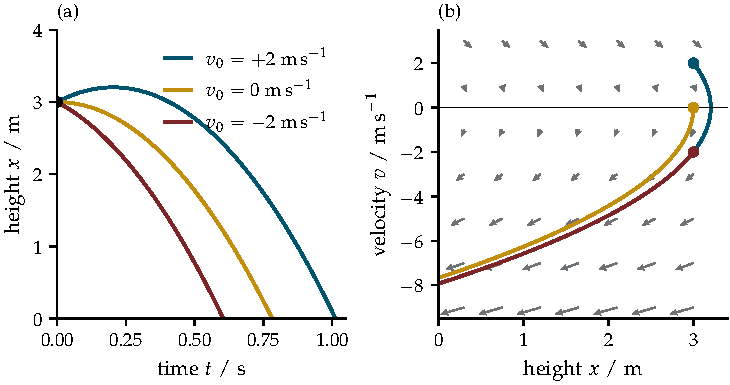
\includegraphics{ch02_newton/state}
\caption{The state of a falling ball. (a) Three balls released
\SI{3}{\metre} above the ground with velocities of $+2$, 0 and
\SI{-2}{\metre\per\second}: the same position with different velocities
gives different motions. (b) The same motions as paths through the
states $(x, v)$. Each grey arrow shows how the state at its tail changes
over \SI{0.03}{\second}, and dots mark the starting states.}
\label{fig:ne-state}
\end{figure}

That each starting state leads to exactly one motion is a theorem of
mathematics, the existence and uniqueness theorem for differential
equations, known as the Picard--Lindel\"of theorem. It holds provided
that $F$ is continuous in time and its slopes with respect to $x$ and
$v$ stay bounded in a neighbourhood of the starting state. It then
guarantees a single solution for at least some interval of time. Smooth
force laws satisfy this condition away from singularities such as two
atoms occupying the same position. A discontinuous cutoff requires
separate care, which is one reason to examine how forces are truncated
in Chapter~8. In three dimensions the same holds
with $\vb{r}$ and $\vb{v}$ in place of $x$ and $v$, and the state is the
pair of vectors $(\vb{r}, \vb{v})$. This is the state of a particle; a
body that can also turn needs, in addition, its orientation and how fast
it is turning (Chapter~5).

\begin{keyidea}
The equation of motion, $m\,\dd^2\vb{r}/\dd t^2 = \vb{F}$, is a
second-order differential equation. Given the force law and the starting
time, the position and velocity together, the state, determine the
motion that follows.
\end{keyidea}

\begin{selfcheck}
Two stones are dropped from rest, one from a bridge and one from a
window \SI{1}{\metre} lower. Do they have the same state at the moment of
release? Do they follow the same motion?
\end{selfcheck}

%=============================================================================!
% 2.7  DRAG AND TERMINAL VELOCITY                                             !
%=============================================================================!
\section{Drag and terminal velocity}
\label{sec:ne-drag}

Drop a small bead into a jar of honey or a thick oil. It speeds up for a
moment and then sinks at a steady speed, however tall the jar. This is
the first force we meet that depends on the velocity, and solving its
equation of motion needs a new function, the exponential. The same
equation returns in Chapter~13, where it describes how a thermostat
steadies the temperature of a simulation.

\subsection*{The drag force}

The liquid resists the motion of the bead with a drag force that points
against the velocity. For small bodies moving slowly through a thick
liquid this force is, to a good approximation, proportional to the
velocity,
\begin{equation*}
   \vb{F}_{\mathrm{drag}} = -b\,\vb{v} ,
\end{equation*}
where the drag coefficient $b$, in kilograms per second, depends on the
size of the body and the thickness of the liquid. Fast bodies moving
through air feel a drag that grows more nearly as the square of the
speed, which we do not treat. The liquid also pushes the bead upwards
with a constant force called buoyancy, equal to the weight of the liquid
that the bead displaces. For a bead much denser than the liquid this is
a small correction, and we neglect it.

\subsection*{The equation of motion}

We measure the depth $x$ downwards, so that the weight $mg$ is positive
and the drag $-bv$ opposes a downward velocity. The second law for the
bead is
\begin{equation*}
   m\,\frac{\dd v}{\dd t} = mg - bv ,
\end{equation*}
and dividing both sides by $m$,
\begin{equation}
   \frac{\dd v}{\dd t} = g - \gamma v, \qquad \gamma = \frac{b}{m} .
   \label{eq:ne-drag}
\end{equation}
The constant $\gamma$, called the drag rate, has units of
$(\si{\kilogram\per\second})/\si{\kilogram} = \si{\per\second}$, an
inverse time; we shall see that $1/\gamma$ sets the time scale on which the
bead settles into its steady motion.

Before solving \cref{eq:ne-drag} we can find the steady speed directly.
The bead stops speeding up when $\dd v/\dd t = 0$, which happens when the
drag has grown to balance the weight,
\begin{equation*}
   0 = g - \gamma v_\infty
   \quad\Longrightarrow\quad
   v_\infty = \frac{g}{\gamma} = \frac{mg}{b} .
\end{equation*}
This steady speed is called the terminal velocity. We write it
$v_\infty$, read `v infinity', because the bead approaches it as the time
grows without limit.

\subsection*{Measuring the velocity from its terminal value}

\Cref{eq:ne-drag} becomes simpler if we follow not the velocity itself
but its distance from the terminal velocity, $w = v - v_\infty$. Since
$v_\infty$ is a constant, $\dd w/\dd t = \dd v/\dd t$, and substituting
$v = w + v_\infty$ into \cref{eq:ne-drag},
\begin{align*}
   \frac{\dd w}{\dd t}
   &= g - \gamma\,(w + v_\infty)
      && \text{substituting for $v$}\\
   &= (g - \gamma v_\infty) - \gamma w
      && \text{multiplying out the bracket}\\
   &= -\gamma w
      && \text{since $\gamma v_\infty = g$.}
\end{align*}
The gap between the velocity and its terminal value therefore shrinks at
a rate proportional to the gap itself: when the gap is large it closes
quickly, and as it narrows it closes ever more slowly. To solve this
equation we need a function whose derivative is a constant times the
function, and the boxes below build it.

\begin{toolbox}[The exponential function]
Define $\mathrm{E}(s)$ as the function that equals its own derivative and
takes the value 1 at $s = 0$,
\begin{equation*}
   \frac{\dd\mathrm{E}}{\dd s} = \mathrm{E}(s), \qquad \mathrm{E}(0) = 1 .
\end{equation*}
Differentiating both sides again shows that the second derivative also
equals $\mathrm{E}$, and so on for every derivative, so at $s = 0$ every
derivative of $\mathrm{E}$ equals 1. The Taylor series of
\cref{sec:mo-taylor} about $s = 0$ is therefore
\begin{equation*}
   \mathrm{E}(s) = 1 + s + \frac{s^2}{2!} + \frac{s^3}{3!} + \dotsb .
\end{equation*}
Differentiating the series term by term confirms that it is its own
derivative: since $n! = n\times(n-1)!$, the term $s^n/n!$ becomes
$n\,s^{n-1}/n! = s^{n-1}/(n-1)!$, the term before it, so the
differentiated series is the same series again. Such a function
therefore exists, and since $\dd\mathrm{E}/\dd s = \mathrm{E}$ is a
first-order differential equation, the uniqueness theorem of
\cref{sec:ne-equations} allows only one with $\mathrm{E}(0) = 1$.
Its value at $s = 1$ is a number called $\mathrm{e}$. Adding the first
seven terms, $1 + 1 + 0.5 + 0.1667 + 0.0417 + 0.0083 + 0.0014 = 2.7181$;
the next three terms, $0.0002$, $0.00002$ and $0.000003$, raise this to
$2.71828$, and later terms are too small to change these digits:
$\mathrm{e} = 2.71828\ldots$.

Now let $\lambda$ be any constant. By the chain rule of
\cref{sec:mo-acceleration}, with inner function $\lambda t$,
\begin{equation*}
   \frac{\dd}{\dd t}\,\mathrm{E}(\lambda t)
   = \mathrm{E}'(\lambda t)\,\lambda = \lambda\,\mathrm{E}(\lambda t) ,
\end{equation*}
the second step using $\mathrm{E}' = \mathrm{E}$,
so $\mathrm{E}(\lambda t)$ is a function whose derivative is $\lambda$
times itself, which is what we need. The series also gives values at
negative $s$, for instance
\begin{equation*}
   \mathrm{E}(-1) = 1 - 1 + 0.5 - 0.1667 + 0.0417 - 0.0083 + 0.0014 - \dotsb
   = 0.368 .
\end{equation*}
\end{toolbox}

\begin{toolbox}[The product rule]
For two functions $p(s)$ and $q(s)$, the change in their product over a
small step $h$ can be split into a change in $p$ and a change in $q$, by
adding and subtracting $p(s)\,q(s+h)$,
\begin{equation*}
   p(s+h)\,q(s+h) - p(s)\,q(s)
   = \bigl[p(s+h) - p(s)\bigr]\,q(s+h) + p(s)\,\bigl[q(s+h) - q(s)\bigr] .
\end{equation*}
Dividing by $h$ and letting $h \to 0$, the brackets divided by $h$ become
the derivatives $p'$ and $q'$, and $q(s+h)$ becomes $q(s)$, so
\begin{equation*}
   \frac{\dd}{\dd s}\bigl(pq\bigr) = p'q + pq' .
\end{equation*}
\end{toolbox}

The product rule shows why $\mathrm{E}$ deserves its usual name. Fix a
number $c$ and consider $f(s) = \mathrm{E}(c + s)\,\mathrm{E}(-s)$. The
derivative of $\mathrm{E}(-s)$ is $-\mathrm{E}(-s)$, by the chain rule
with $\lambda = -1$, and the derivative of $\mathrm{E}(c + s)$ is
$\mathrm{E}(c + s)$, by the chain rule with inner function $c + s$, whose
derivative is 1, so
\begin{align*}
   f'(s) &= \mathrm{E}(c+s)\,\mathrm{E}(-s)
      + \mathrm{E}(c+s)\,\bigl[-\mathrm{E}(-s)\bigr]
      && \text{by the product rule}\\
   &= 0 .
\end{align*}
A function whose derivative is zero everywhere does not change, by
\cref{eq:mo-integrals} (with $f$ in place of $v$ and $f' = 0$ in place
of $a$, it reads $f(s) = f(0) + \int_0^s 0\,\dd s' = f(0)$), so $f$ keeps its value at $s = 0$, which is
$\mathrm{E}(c)\,\mathrm{E}(0) = \mathrm{E}(c)$. Setting $c = 0$ gives
$\mathrm{E}(s)\,\mathrm{E}(-s) = 1$, and dividing $\mathrm{E}(c+s)\,
\mathrm{E}(-s) = \mathrm{E}(c)$ by $\mathrm{E}(-s)$, which is the same as
multiplying by $\mathrm{E}(s)$,
\begin{equation*}
   \mathrm{E}(c + s) = \mathrm{E}(c)\,\mathrm{E}(s) .
\end{equation*}
This is the rule obeyed by powers, $\mathrm{e}^{c+s} =
\mathrm{e}^c\,\mathrm{e}^s$. Applying it with $c = s = 1$ gives
$\mathrm{E}(2) = \mathrm{e}^2$, then $\mathrm{E}(3) = \mathrm{e}^3$, and
so on, and $\mathrm{E}(-s) = 1/\mathrm{E}(s)$ matches $\mathrm{e}^{-s} =
1/\mathrm{e}^s$. Two further facts follow. Since $\mathrm{E}(s)\,
\mathrm{E}(-s) = 1$, $\mathrm{E}$ is never zero, and since $\mathrm{E}(s)
= \mathrm{E}(\tfrac s2)^2$, by the rule with both $c$ and $s$ set to
$\tfrac s2$, it is never negative; so $\mathrm{E}(s) > 0$ for every $s$.
Its derivative, equal to itself, is then positive too, so $\mathrm{E}$
rises steadily and never takes the same value at two different $s$.
Fractions agree with powers as well: $\mathrm{E}(\tfrac12)^2 =
\mathrm{E}(\tfrac12 + \tfrac12) = \mathrm{E}(1) = \mathrm{e}$, so
$\mathrm{E}(\tfrac12) = \sqrt{\mathrm{e}} = \mathrm{e}^{1/2}$, the positive
root. The
function $\mathrm{E}$ therefore extends the powers of $\mathrm{e}$ to
every real number, and from now on we write it $\mathrm{e}^s$, the
exponential function. Because it never takes a value twice, it can be
undone: its inverse is the natural logarithm, $\ln$, defined by
$\ln(\mathrm{e}^s) = s$. It is not the base-10 logarithm $\log$ of
\cref{sec:mo-taylor}; calculators mark it `ln'.

The rule for sums also explains how a decaying exponential decays.
Lowering $s$ by one multiplies the function by a fixed factor,
$\mathrm{e}^{s-1} = \mathrm{e}^s\,\mathrm{e}^{-1} = 0.368\,\mathrm{e}^s$.
In $\mathrm{e}^{\lambda t}$ with negative $\lambda$ the exponent $s =
\lambda t$ falls by $\lambda\times(1/\lvert\lambda\rvert) = -1$ each time
$t$ grows by $1/\lvert\lambda\rvert$, so the function falls to about
\SI{37}{\percent} of its value over every such interval, wherever it
starts.

\subsection*{Solving the equation}

The gap obeys $\dd w/\dd t = -\gamma w$, and by the toolbox, with
$\lambda = -\gamma$, the function $w = C\,\mathrm{e}^{-\gamma t}$ has
derivative $-\gamma C\,\mathrm{e}^{-\gamma t} = -\gamma w$ for any
constant $C$. At $t = 0$ the exponential is 1, so $C$ is the starting gap,
$C = v_0 - v_\infty$, where $v_0$ is the velocity at release. Here the
force depends on the velocity alone, so the second of
\cref{eq:ne-first-order} involves $v$ alone, and by the uniqueness
theorem of \cref{sec:ne-equations} the starting velocity fixes its
solution. We have therefore found it, and adding $v_\infty$ back,
\begin{equation}
   v(t) = v_\infty + (v_0 - v_\infty)\,\mathrm{e}^{-\gamma t} .
   \label{eq:ne-drag-v}
\end{equation}
Whatever the starting velocity, the gap shrinks to $\mathrm{e}^{-1} =
\SI{37}{\percent}$ of its size every interval $1/\gamma$, and the
velocity approaches $v_\infty$ from below if the bead starts slower and
from above if it starts faster. A bead released from rest has $v_0 = 0$,
and then $v(t) = v_\infty\,(1 - \mathrm{e}^{-\gamma t})$.

As an example, take a bead of mass \SI{0.01}{\kilogram} with a drag
coefficient of \SI{0.05}{\kilogram\per\second}. Then $\gamma = 0.05/0.01
= \SI{5}{\per\second}$, so $1/\gamma = \SI{0.2}{\second}$, and the
terminal velocity is $v_\infty = 9.80665/5 = \SI{1.961}{\metre\per
\second}$. These values are chosen so that the approach is easy to see
on a scale of seconds. A real bead this heavy and this fast would feel a
drag that is not proportional to its speed, while for the small, slow
beads to which the linear law applies the whole approach is over in a
small fraction of a second. Released from rest, the bead's velocity as a
fraction of $v_\infty$ is $1 - \mathrm{e}^{-\gamma t}$, where
$\mathrm{e}^{-2} = 0.368^2$, $\mathrm{e}^{-3} = 0.368^3$ and
$\mathrm{e}^{-5} = 0.368^5$ by the rule for sums:
\begin{center}
\begin{tabular}{cccc}
\toprule
$t$ / \si{\second} & $\gamma t$ & $\mathrm{e}^{-\gamma t}$
   & $v/v_\infty = 1 - \mathrm{e}^{-\gamma t}$\\
\midrule
0.2 & 1 & 0.368 & \SI{63.2}{\percent}\\
0.4 & 2 & 0.135 & \SI{86.5}{\percent}\\
0.6 & 3 & 0.050 & \SI{95.0}{\percent}\\
1.0 & 5 & 0.007 & \SI{99.3}{\percent}\\
\bottomrule
\end{tabular}
\end{center}
To find when it reaches \SI{90}{\percent} of $v_\infty$, we need
$\mathrm{e}^{-\gamma t} = 0.1$. Taking the natural logarithm of both
sides gives $-\gamma t = \ln 0.1 = -2.303$, the value of the logarithm
coming from a calculator, so $t = 2.303/5 =
\SI{0.461}{\second}$ (\cref{fig:ne-drag}a).

\subsection*{The distance fallen}

The depth follows by integrating the velocity, as in
\cref{sec:mo-integrating}. The function $-\mathrm{e}^{-\gamma t'}/\gamma$
has derivative $\mathrm{e}^{-\gamma t'}$, by the toolbox with $\lambda =
-\gamma$, so
\begin{equation*}
   \int_0^t \mathrm{e}^{-\gamma t'}\,\dd t'
   = \Bigl[-\frac{\mathrm{e}^{-\gamma t'}}{\gamma}\Bigr]_0^t
   = \frac{1 - \mathrm{e}^{-\gamma t}}{\gamma} ,
\end{equation*}
and for a bead released from rest at $x = 0$,
\begin{equation}
   x(t) = \int_0^t v_\infty\bigl(1 - \mathrm{e}^{-\gamma t'}\bigr)\,\dd t'
   = v_\infty\,t - \frac{v_\infty}{\gamma}\,\bigl(1 -
   \mathrm{e}^{-\gamma t}\bigr) .
   \label{eq:ne-drag-x}
\end{equation}
Two limits check this result. Long after release the exponential has
died away and $x \approx v_\infty t - v_\infty/\gamma$: the bead sinks at
its terminal velocity, but a fixed distance $v_\infty/\gamma$ behind
where it would be had it moved at that velocity from the start, because
it spent its first moments speeding up. For the example bead this lag is
$1.961/5 = \SI{0.392}{\metre}$. Just after release, when $\gamma t$ is
small, the exponential series with $s = -\gamma t$ gives
$\mathrm{e}^{-\gamma t} = 1 - \gamma t + \tfrac12\gamma^2 t^2 +
\order{t^3}$, so $1 - \mathrm{e}^{-\gamma t} = \gamma t - \tfrac12\gamma^2
t^2 + \order{t^3}$, with $\order{t^3}$ as in
\cref{sec:mo-taylor}, and substituting into
\cref{eq:ne-drag-x},
\begin{align*}
   x(t) &= v_\infty t - \frac{v_\infty}{\gamma}\Bigl(\gamma t
      - \tfrac12\gamma^2 t^2\Bigr) + \order{t^3}\\
   &= v_\infty t - v_\infty t + \tfrac12 v_\infty\gamma\, t^2 + \order{t^3}
      && \text{multiplying out the bracket}\\
   &= \tfrac12 g t^2 + \order{t^3}
      && \text{since $v_\infty\gamma = g$.}
\end{align*}
At first the bead is moving too slowly for the drag to matter, and it
falls freely. For the example bead, after \SI{0.02}{\second} it has
fallen \SI{1.898}{\milli\metre} against \SI{1.961}{\milli\metre} in free
fall; after \SI{0.1}{\second}, \SI{41.79}{\milli\metre} against
\SI{49.03}{\milli\metre}; and after a second, \SI{1.572}{\metre} against
\SI{4.903}{\metre} (\cref{fig:ne-drag}b).

\begin{figure}[htb]
\centering
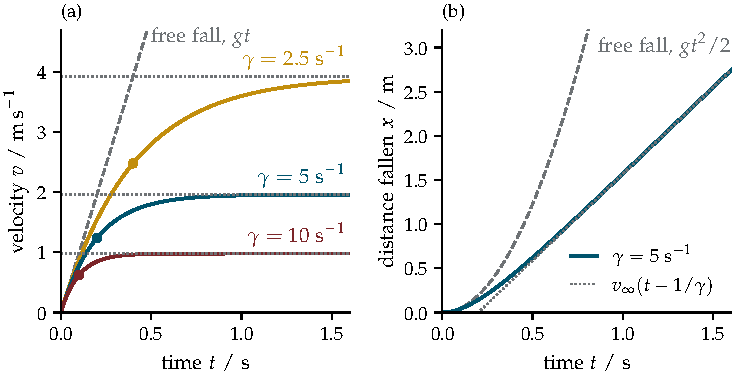
\includegraphics{ch02_newton/drag}
\caption{Falling from rest with a drag proportional to the velocity. (a)
Velocity for three drag rates $\gamma$, approaching the terminal velocity
$v_\infty = g/\gamma$ (dotted), against free fall (dashed); dots mark $t
= 1/\gamma$, where \SI{63}{\percent} of the terminal velocity is reached.
(b) Distance fallen for $\gamma = \SI{5}{\per\second}$, which follows
free fall at first and then the line $v_\infty(t - 1/\gamma)$.}
\label{fig:ne-drag}
\end{figure}

\notebook{02}{change the mass and drag coefficient and watch the approach
to terminal velocity}

\begin{selfcheck}
A bead is fired downwards into the honey faster than its terminal
velocity. Does it speed up or slow down? Sketch its velocity against
time.
\end{selfcheck}

%=============================================================================!
% 2.8  THE SPRING                                                             !
%=============================================================================!
\section{The spring}
\label{sec:ne-spring}

A block fixed to a spring and pulled aside swings back and forth about
its resting place. This motion recurs throughout the book because an atom
displaced slightly from a stable position feels a similar restoring
force from its neighbours. Chapter~4 develops that connection; here we derive the
motion from the second law.

\subsection*{Hooke's law}

Lay a spring on a smooth table, fix one end to a wall and attach a block
of mass $m$ to the other. We measure the position $x$ of the block from
its resting place, where the spring has its natural length, so that $x$
is the stretch of the spring: positive when it is stretched, negative
when it is squashed. A stretched spring pulls the block back towards the
wall, and a squashed one pushes it away (\cref{fig:ne-spring-states}).
Measurements with a spring balance show that, for stretches small
compared with the length of the spring, the force is proportional to the
stretch,
\begin{equation*}
   F = -kx .
\end{equation*}
This is Hooke's law. The stiffness $k$, in newtons per metre, measures how
hard the spring is to stretch, and the minus sign records that the force
always points back towards $x = 0$, against the stretch. A spring with $k
= \SI{50}{\newton\per\metre}$ needs a force of \SI{1}{\newton} to stretch
it by $1/50 = \SI{0.02}{\metre}$, or \SI{2}{\centi\metre}.

\begin{figure}[htb]
\centering
\begin{tikzpicture}[line cap=round,
   force/.style={-{Stealth[length=5pt]}, line width=1.1pt, accent},
   stretch/.style={{Stealth[length=3pt]}-{Stealth[length=3pt]},
      line width=0.4pt},
   coil/.style={decorate, decoration={coil, aspect=0.45,
      segment length=4pt, amplitude=3.5pt, pre length=3pt,
      post length=3pt}, line width=0.6pt}]
   % one row per state; \x is the stretch, in the units of the drawing
   \foreach \row/\x/\name in {0/-0.6/squashed, 1/0/natural length,
      2/0.8/stretched} {
      \begin{scope}[yshift=-\row*1.9cm]
         \fill[black!35] (-0.12,-0.35) rectangle (0,0.45);
         \draw[line width=0.6pt] (0,-0.35) -- (6.0,-0.35);
         \draw[coil] (0,0.05) -- (3.0+\x,0.05);
         \draw[line width=0.6pt, fill=black!8] (3.0+\x,-0.35)
            rectangle (3.8+\x,0.45);
         \node[anchor=west] at (6.3,0.05) {\small \name};
      \end{scope}
   }
   % the resting place of the block's left face
   \draw[dashed, black!50, line width=0.5pt] (3.0,1.3) -- (3.0,-4.6);
   \node[above] at (3.0,1.3) {\small $x = 0$};
   % the force of the spring on the block, drawn above it
   \draw[force] (2.6,0.8) -- (3.5,0.8) node[right] {\small $F$};
   \draw[force] (4.7,-3.0) -- (3.8,-3.0) node[left] {\small $F$};
   % the stretch, measured from the resting place
   \draw[stretch] (3.0,-0.65) -- (2.4,-0.65)
      node[left] {\scriptsize $x < 0$};
   \draw[stretch] (3.0,-4.45) -- (3.8,-4.45)
      node[right] {\scriptsize $x > 0$};
\end{tikzpicture}
\caption{A block on a spring. Squashed ($x < 0$), the spring pushes the
block away from the wall; at its natural length ($x = 0$) it exerts no
force; stretched ($x > 0$), it pulls the block back. In each case the
force (teal) points towards $x = 0$, against the stretch.}
\label{fig:ne-spring-states}
\end{figure}

\subsection*{The equation of motion}

Vertically, the weight of the block is balanced by the push of the table,
called the normal force because it acts at right angles to the surface,
which mathematicians call normal to it. Along the table the spring is the
only force, so the second law reads $m\,\dd^2 x/\dd t^2 = -kx$, and
dividing by $m$,
\begin{equation}
   \frac{\dd^2 x}{\dd t^2} = -\frac{k}{m}\,x .
   \label{eq:ne-spring}
\end{equation}
Rather than solve this equation from nothing, we recognise it. In
\cref{sec:mo-trig} we found that every sinusoid obeys $\dd^2 x/\dd t^2 =
-\omega^2 x$, which is \cref{eq:ne-spring} if $\omega^2 = k/m$. With
$\omega = \sqrt{k/m}$, both $\cos\omega t$ and $\sin\omega t$ are such
sinusoids, and the equation is obeyed also by any combination
\begin{equation*}
   x(t) = c_1\cos\omega t + c_2\sin\omega t
\end{equation*}
with constant $c_1$ and $c_2$. Differentiating twice with the chain rule
confirms it,
\begin{align*}
   \frac{\dd x}{\dd t} &= -c_1\omega\sin\omega t + c_2\omega\cos\omega t ,\\
   \frac{\dd^2 x}{\dd t^2} &= -c_1\omega^2\cos\omega t
      - c_2\omega^2\sin\omega t
      && \text{differentiating again}\\
   &= -\omega^2 x = -\frac{k}{m}\,x
      && \text{taking out the common factor $-\omega^2$,}
\end{align*}
so \cref{eq:ne-spring} holds whatever the values of $c_1$ and $c_2$.

\subsection*{Matching the starting state}

The two constants are fixed by the state at $t = 0$. Since $\cos 0 = 1$
and $\sin 0 = 0$, setting $t = 0$ in $x$ and $\dd x/\dd t$ gives $x_0 =
c_1$ and $v_0 = c_2\omega$, where $x_0$ and $v_0$ are the starting position
and velocity. The motion is therefore
\begin{equation}
   x(t) = x_0\cos\omega t + \frac{v_0}{\omega}\,\sin\omega t .
   \label{eq:ne-spring-solution}
\end{equation}
Every starting state $(x_0, v_0)$ is matched in this way, so by the
uniqueness of solutions (\cref{sec:ne-equations})
\cref{eq:ne-spring-solution} is the motion for every start. With $x_0 =
v_0 = 0$ it gives $x = 0$ for all time: a block at rest at its resting
place stays there.

The same motion can be written as a single sinusoid, which shows at a
glance how far the block swings. We write it with a cosine,
\begin{equation*}
   x(t) = A\cos(\omega t + \phi) ,
\end{equation*}
which by the quarter-turn relation $\cos\theta = \sin(\theta + \pi/2)$ is
the sinusoid of \cref{eq:mo-sinusoid} with its phase larger by $\pi/2$.
Expanding it with the addition formula \cref{eq:mo-addition},
\begin{equation*}
   A\cos(\omega t + \phi) = A\cos\phi\,\cos\omega t - A\sin\phi\,\sin\omega t ,
\end{equation*}
which is \cref{eq:ne-spring-solution} when the coefficients of $\cos\omega
t$ and $\sin\omega t$ agree,
\begin{equation*}
   A\cos\phi = x_0, \qquad A\sin\phi = -\frac{v_0}{\omega} .
\end{equation*}
To find $A$, we square both equations and add them, using $\cos^2\phi +
\sin^2\phi = 1$:
\begin{equation*}
   x_0^2 + \Bigl(\frac{v_0}{\omega}\Bigr)^2
   = A^2\bigl(\cos^2\phi + \sin^2\phi\bigr) = A^2
   \quad\Longrightarrow\quad
   A = \sqrt{x_0^2 + (v_0/\omega)^2} .
\end{equation*}
If $A = 0$ the block rests at $x = 0$ and the phase plays no part.
Otherwise the two equations give $\cos\phi = x_0/A$ and $\sin\phi =
-v_0/(\omega A)$. Together these fix the point $(\cos\phi, \sin\phi)$ on
the unit circle, and so fix $\phi$ up to whole turns of $2\pi$. The
arcsine of \cref{sec:mo-trig} returns the angle between $-\pi/2$ and
$\pi/2$ with the right sine; the cosine of that angle is never negative,
and by $\cos^2 + \sin^2 = 1$ it equals $+\sqrt{1 - \sin^2\phi}$, which is
$\cos\phi$ itself when $\cos\phi \ge 0$. In that case, therefore, $\phi =
\arcsin(\sin\phi)$.
When $\cos\phi < 0$ the angle is $\pi - \arcsin(\sin\phi)$ instead, which
has the same sine, since $\sin(\pi - \theta) = \sin\theta$, and a
negative cosine, since $\cos(\pi - \theta) = -\cos\theta$. The sign of
the cosine thus selects between the two angles that share a sine.

Take a block of \SI{0.5}{\kilogram} on the spring of
\SI{50}{\newton\per\metre}, so that $\omega = \sqrt{50/0.5} =
\SI{10}{\radian\per\second}$, and start it \SI{3}{\centi\metre} from its
resting place, moving outwards, away from the wall, at
\SI{0.4}{\metre\per\second}. In metres,
$x_0 = 0.03$ and $v_0/\omega = 0.04$, so $x(t) = 0.03\cos 10t +
0.04\sin 10t$ by \cref{eq:ne-spring-solution}, and
\begin{align*}
   A &= \sqrt{0.03^2 + 0.04^2} = \SI{0.05}{\metre} ,\\
   \cos\phi &= 0.03/0.05 = 0.6, \qquad
   \sin\phi = -0.04/0.05 = -0.8 .
\end{align*}
The block swings out to \SI{5}{\centi\metre} before turning back. The
cosine is positive, so $\phi = \arcsin(-0.8) = \SI{-0.927}{\radian}$.
Started instead \SI{3}{\centi\metre} on the wall side, $x_0 = -0.03$,
with the same velocity, the block has the same amplitude, but $\cos\phi =
-0.6$ is negative, so $\phi = \pi - \arcsin(-0.8) = \pi + 0.927 =
\SI{4.069}{\radian}$.

\subsection*{The period and the motion}

The block repeats its motion when $\omega t$ grows by $2\pi$, so its
angular frequency and period are
\begin{equation}
   \omega = \sqrt{\frac{k}{m}}, \qquad
   \frac{2\pi}{\omega} = 2\pi\sqrt{\frac{m}{k}} .
   \label{eq:ne-spring-omega}
\end{equation}
A heavier block oscillates more slowly and a stiffer spring more quickly.
As long as Hooke's law holds, the period does not depend on the
amplitude, and there is a simple reason.
Pull the block twice as far and the spring pulls twice as hard, so at
every stage the acceleration is twice as large; the block covers twice the
distance at twice the speed and takes the same time. In the language of
the equation, if $x(t)$ solves \cref{eq:ne-spring} then so does $2x(t)$,
because both sides double.

\Cref{fig:ne-spring} shows the simplest start of all, the same block
pulled out \SI{4}{\centi\metre} and released from rest, for which $\phi
= 0$, since then $x_0 = A$ and $v_0 = 0$. The period is $2\pi/10 =
\SI{0.628}{\second}$. On the way in, the spring pulls the block in the
direction it is moving, so the block speeds up all the way to the centre;
past the centre the spring pulls against the motion and slows it. The
speed is therefore largest at $x = 0$. Differentiating $x = A\cos(\omega
t + \phi)$ with the chain rule gives $\dd x/\dd t = -A\omega\sin(\omega t
+ \phi)$; where $x = 0$ the cosine is zero, so the sine is $\pm1$ by
$\cos^2 + \sin^2 = 1$, and the speed there is $A\omega = 0.04\times 10 =
\SI{0.4}{\metre\per\second}$. At the turning points, $x = \pm A$, the
block is momentarily at rest, yet its acceleration there, $-\omega^2 x =
\mp A\omega^2 = \mp\SI{4}{\metre\per\second\squared}$ by
\cref{eq:ne-spring}, is the largest it ever has, since $\lvert x\rvert$
never exceeds $A$. This is the top of the throw of \cref{sec:mo-acceleration} again:
zero velocity does not mean zero acceleration.

\begin{figure}[htb]
\centering
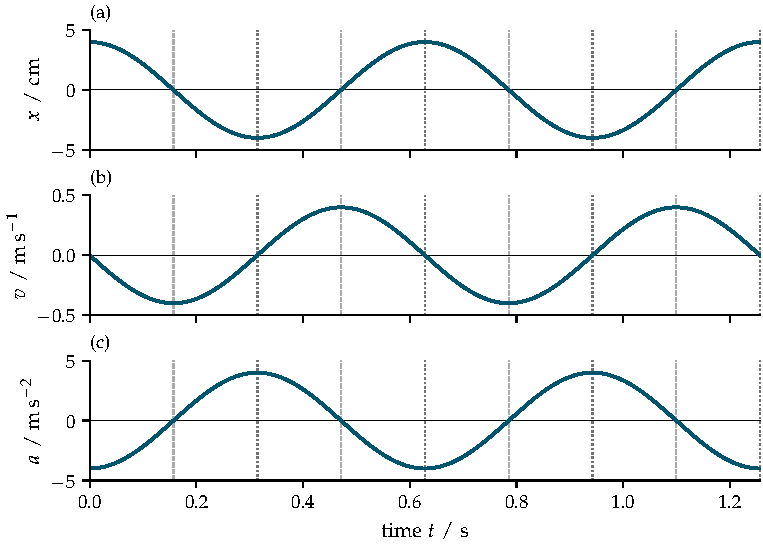
\includegraphics{ch02_newton/spring}
\caption{A block of \SI{0.5}{\kilogram} on a spring of
\SI{50}{\newton\per\metre}, released from rest \SI{4}{\centi\metre} from
its resting place, over two periods. (a) Position, (b) velocity and (c)
acceleration. At the dotted lines the block turns: its velocity is zero
and its acceleration largest. At the dashed lines it passes the centre:
its speed is largest and its acceleration zero.}
\label{fig:ne-spring}
\end{figure}

\notebook{02}{change the mass, stiffness and starting state of the block}

\begin{selfcheck}
A block oscillates on a spring with a period of \SI{1}{\second}. What is
the period if the mass is made four times larger? What if the block is
pulled out twice as far before release?
\end{selfcheck}

%=============================================================================!
% 2.9  SEVERAL BODIES: MOMENTUM AND THE CENTRE OF MASS                        !
%=============================================================================!
\section{Several bodies: momentum and the centre of mass}
\label{sec:ne-bodies}

So far each body has moved under forces from its surroundings. When
several bodies push and pull on one another, as the atoms of a material
do, the third law ties their motions together. This section shows how,
using a new quantity, momentum, and a new point, the centre of mass.

\subsection*{Momentum}

The momentum of a body is its mass times its velocity,
\begin{equation*}
   \vb{p} = m\vb{v} ,
\end{equation*}
a vector in \si{\kilogram\metre\per\second} that points along the
velocity. Since the mass is constant, the rate of change of the momentum
is $\dd\vb{p}/\dd t = m\,\dd\vb{v}/\dd t = m\vb{a}$, and the second law
can be written
\begin{equation*}
   \frac{\dd\vb{p}}{\dd t} = \vb{F} :
\end{equation*}
the net force on a body is the rate at which its momentum changes. A
constant force $\vb{F}$ acting from $t = 0$ to a time $t$ therefore
changes the momentum by $\vb{F}t$, since $\vb{p}$ then grows at the
constant rate $\vb{F}$, as $v$ grows by $at$ at the constant rate $a$ in
\cref{eq:mo-constant}; so the momentum of a body measures how long
a given force must push to bring it from rest to its velocity, or to stop
it again. A trolley of \SI{20}{\kilogram} pushed from rest by
\SI{10}{\newton} for \SI{2}{\second} gains a momentum of $10\times2 =
\SI{20}{\kilogram\metre\per\second}$, and so a velocity of $20/20 =
\SI{1}{\metre\per\second}$. A lorry and a bicycle moving at the same
speed have very different momenta, and the brakes of the lorry must push
far harder, or for far longer, to stop it.

\subsection*{Two carts}

Two carts, of masses $m_1 = \SI{1}{\kilogram}$ and $m_2 =
\SI{3}{\kilogram}$, stand at rest on a level, smooth track with a
compressed spring between them, and are released
(\cref{fig:ne-carts-sketch}). On each cart the weight and the normal
force balance, so only the forces along the track matter, and these come
from the spring. The spring is light, and we treat it as having no mass.
Two steps then fix the forces on the carts. First, the net force on the
spring must be zero, since by the second law any net force on a body of
no mass would give it an unlimited acceleration; so the two carts push on
the two ends of the spring with forces of equal size. Second, by the third
law, the spring pushes back on each cart with a force of that same size:
$-\vb{F}$ on the first cart, backwards, and $+\vb{F}$ on the second,
forwards.

\begin{figure}[htb]
\centering
\begin{tikzpicture}[line cap=round,
   force/.style={-{Stealth[length=5pt]}, line width=1.1pt, accent},
   coil/.style={decorate, decoration={coil, aspect=0.45,
      segment length=3pt, amplitude=3.5pt, pre length=2pt,
      post length=2pt}, line width=0.6pt}]
   \draw[line width=0.6pt] (-0.6,0) -- (7.4,0);
   % cart 1, the lighter, and cart 2, the heavier
   \draw[line width=0.6pt, fill=black!8] (0.6,0.18) rectangle (1.8,0.9);
   \draw[line width=0.6pt, fill=black!8] (3.6,0.18) rectangle (6.0,1.2);
   \foreach \x in {0.85,1.55,4.0,5.6}
      \draw[line width=0.6pt, fill=white] (\x,0.09) circle (0.09);
   \draw[coil] (1.8,0.5) -- (3.6,0.5);
   \node at (1.2,0.54) {\small 1};
   \node at (4.8,0.69) {\small 2};
   % the push of the spring on each cart
   \draw[force] (0.6,0.54) -- (-0.4,0.54) node[above] {\small $-\vb{F}$};
   \draw[force] (6.0,0.69) -- (7.0,0.69) node[above] {\small $+\vb{F}$};
   \node[below] at (1.2,-0.05) {\small \SI{1}{\kilogram}};
   \node[below] at (4.8,-0.05) {\small \SI{3}{\kilogram}};
\end{tikzpicture}
\caption{Two carts at rest with a compressed spring between them. The
spring pushes the two carts with forces of equal size in opposite
directions (teal); the weights and normal forces, which balance on each
cart, are not drawn.}
\label{fig:ne-carts-sketch}
\end{figure}

Applying the second law to each cart and adding the two equations,
\begin{equation*}
   \frac{\dd\vb{p}_1}{\dd t} = -\vb{F}, \qquad
   \frac{\dd\vb{p}_2}{\dd t} = +\vb{F}
   \quad\Longrightarrow\quad
   \frac{\dd}{\dd t}\bigl(\vb{p}_1 + \vb{p}_2\bigr) = -\vb{F} + \vb{F}
   = \vb{0} .
\end{equation*}
The total momentum $\vb{P} = \vb{p}_1 + \vb{p}_2$ therefore does not
change, however the force of the spring varies, and since the carts
started at rest it stays zero. A quantity that keeps the same value as
time passes is said to be conserved, and here the total momentum is
conserved. The carts therefore always have equal and opposite momenta,
$m_1\vb{v}_1 = -m_2\vb{v}_2$, and the lighter cart moves faster by the
ratio of the masses, three times faster here.

\Cref{fig:ne-carts} shows the motion computed for a spring of stiffness
\SI{200}{\newton\per\metre} compressed by \SI{10}{\centi\metre}. The
spring is not fixed to either cart, so once it reaches its natural length
it could only stay in contact by pulling, which a loose spring cannot do,
and it falls away after about \SI{0.096}{\second}, a time found, like
the speeds below, by a computer solution. From then on no force
acts along the track, and by the first law the carts coast apart at
constant velocities, \SI{-1.225}{\metre\per\second} and
\SI{+0.408}{\metre\per\second}, a ratio of exactly $-3$. Their momenta,
$\mp\SI{1.225}{\kilogram\metre\per\second}$, add to zero at every
instant. Chapter~3 shows how energy gives these speeds directly.

\begin{figure}[htb]
\centering
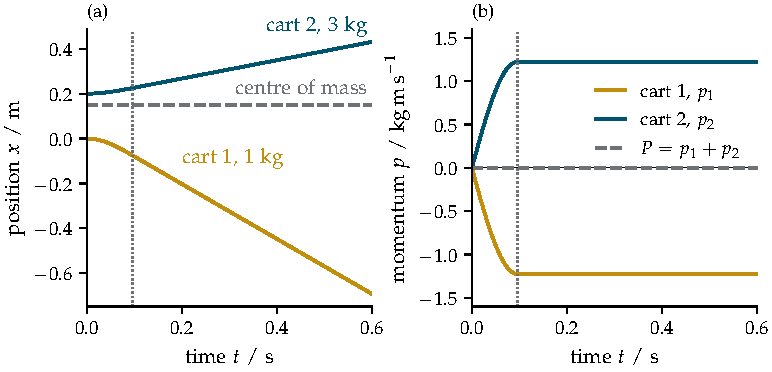
\includegraphics{ch02_newton/carts}
\caption{The carts of \cref{fig:ne-carts-sketch} pushed apart by a
spring of \SI{200}{\newton\per\metre} compressed by
\SI{10}{\centi\metre}; the spring falls away at the dotted line. (a)
Positions of the carts and of their centre of mass (dashed). (b) Momenta
of the carts and the component $P$ of their total momentum along the
track (dashed), which stays zero.}
\label{fig:ne-carts}
\end{figure}

\subsection*{Many bodies}

The same argument works for any number of bodies. The forces on each body
are of two kinds. External forces come from outside the group, such as
the weight of a cart, and we write the net external force on body $i$ as
$\vb{F}_i^{\mathrm{ext}}$. Internal forces come from the other members,
and we write the force on body $i$ from body $j$ as $\vb{F}_{ij}$. For
three bodies, with total momentum $\vb{P} = \vb{p}_1 + \vb{p}_2 +
\vb{p}_3$, adding the three second laws and then regrouping the
internal forces by pairs gives
\begin{align*}
   \frac{\dd\vb{P}}{\dd t}
   &= \frac{\dd\vb{p}_1}{\dd t} + \frac{\dd\vb{p}_2}{\dd t}
      + \frac{\dd\vb{p}_3}{\dd t}\\
   &= \bigl(\vb{F}_1^{\mathrm{ext}} + \vb{F}_{12} + \vb{F}_{13}\bigr)
      + \bigl(\vb{F}_2^{\mathrm{ext}} + \vb{F}_{21} + \vb{F}_{23}\bigr)
      + \bigl(\vb{F}_3^{\mathrm{ext}} + \vb{F}_{31} + \vb{F}_{32}\bigr)\\
   &= \vb{F}^{\mathrm{ext}}
      + \bigl(\vb{F}_{12} + \vb{F}_{21}\bigr)
      + \bigl(\vb{F}_{13} + \vb{F}_{31}\bigr)
      + \bigl(\vb{F}_{23} + \vb{F}_{32}\bigr) ,
\end{align*}
where $\vb{F}^{\mathrm{ext}} = \vb{F}_1^{\mathrm{ext}} +
\vb{F}_2^{\mathrm{ext}} + \vb{F}_3^{\mathrm{ext}}$ is the total external
force. By the third law each bracket is zero. With $N$ bodies, numbered
$i = 1, \dots, N$, the total momentum is $\vb{P} = \vb{p}_1 + \dotsb +
\vb{p}_N$, written $\sum_{i=1}^{N}\vb{p}_i$ with the summation sign of
\cref{sec:mo-integrating}, and the regrouping is the same: every internal force $\vb{F}_{ij}$ meets its
partner $\vb{F}_{ji}$, each pair cancels, and
\begin{equation}
   \frac{\dd\vb{P}}{\dd t} = \vb{F}^{\mathrm{ext}} .
   \label{eq:ne-momentum}
\end{equation}
The internal forces, however strong and however complicated, cannot
change the total momentum. Whenever the total external force is zero,
the total momentum is conserved. That happens when the external forces
cancel, as the weights and normal forces of the carts do, and also when
there are no external forces at all, in which case the group is called
isolated.

\subsection*{The centre of mass}

The group as a whole has a position of its own, the centre of mass, an
average of the positions of its members in which each counts in
proportion to its mass,
\begin{equation*}
   \vb{R} = \frac{1}{M}\sum_{i=1}^{N} m_i\vb{r}_i, \qquad
   M = \sum_{i=1}^{N} m_i ,
\end{equation*}
where $M$ is the total mass. For two bodies on a line it is the balance
point: a light rod carrying the two carts would balance on a pivot placed
there. The centres of the carts start at $x = 0$ and $x =
\SI{0.2}{\metre}$, so their
centre of mass is at $(1\times0 + 3\times0.2)/4 = \SI{0.15}{\metre}$,
nearer the heavier cart. Its motion follows in three lines,
\begin{align*}
   M\vb{R} &= \sum_{i=1}^{N} m_i\vb{r}_i
      && \text{multiplying by $M$}\\
   M\,\frac{\dd\vb{R}}{\dd t} &= \sum_{i=1}^{N} m_i\vb{v}_i = \vb{P}
      && \text{differentiating term by term, the masses constant}\\
   M\,\frac{\dd^2\vb{R}}{\dd t^2} &= \frac{\dd\vb{P}}{\dd t}
      = \vb{F}^{\mathrm{ext}}
      && \text{differentiating again, by \cref{eq:ne-momentum}.}
\end{align*}
The centre of mass moves as a single body of mass $M$ would under the
external forces alone. For the carts there is no external force along the
track, so the centre of mass stays at \SI{0.15}{\metre} while the carts
fly apart (\cref{fig:ne-carts}a). A firework that bursts in flight shows
the same thing in two dimensions: the pieces scatter in every direction,
but until the first of them lands, their centre of mass carries on along
the parabola that the unburst firework would have followed. The only
external force is still the weight, $\vb{F}^{\mathrm{ext}} = \sum_i
m_i\vb{g} = M\vb{g}$, so $\dd^2\vb{R}/\dd t^2 = \vb{g}$ as before the
burst, and the internal forces of the burst change neither $\vb{R}$ nor
$\dd\vb{R}/\dd t = \vb{P}/M$. Chapter~7 shows that the
conservation of momentum follows from a symmetry, that the laws of motion
are the same at every place.

\begin{keyidea}
Internal forces cancel in pairs by the third law, so the total momentum
of a group changes only through external forces, and is conserved when
they add to zero. The centre of mass moves as a single body under the
external forces alone.
\end{keyidea}

\notebook{02}{change the mass ratio of the carts; the centre of mass never
moves}

\begin{selfcheck}
A skater of \SI{60}{\kilogram} standing on smooth ice throws a ball of
\SI{0.5}{\kilogram} forwards at \SI{12}{\metre\per\second}, measured
relative to the ice. What is the
skater's velocity afterwards?
\end{selfcheck}

%=============================================================================!
% 2.10  FROM BALLS TO ATOMS                                                   !
%=============================================================================!
\section{From balls to atoms}
\label{sec:ne-atoms}

Every law of this chapter was found with balls, carts and springs. This
section applies the same laws to atoms and writes them in the form, and in
the units, that molecular dynamics uses.

Atoms are, strictly, quantum objects, and quantum mechanics rather than
Newton's laws describes them exactly. The nuclei, however, are thousands
of times heavier than the electrons, and this book treats them as
classical bodies obeying the second law, while quantum mechanics is used
only to compute the forces on them (Chapter~8). Treating the nuclei
classically is an approximation. It is least accurate for the lightest
nuclei, and for hydrogen the quantum character of the nuclear motion can
change measured properties even at room temperature; Chapter~8 discusses
when the classical picture is adequate.

\subsection*{The equations of motion of $N$ atoms}

Each atom $i$, numbered from 1 to $N$, has a mass $m_i$, a position
$\vb{r}_i$ and a velocity $\vb{v}_i$, and feels a force $\vb{F}_i$ from
the other atoms. We write $\vb{r}^N$ for the whole list of positions,
$\vb{r}_1, \dots, \vb{r}_N$. In the models of this book the force on an
atom depends on where every atom is, but not on how fast the atoms move,
until the thermostats of Chapter~13 add a drag. Before then it is a
function of $\vb{r}^N$ alone, and Chapter~8 explains where it comes
from. The second law for each atom gives
\begin{equation}
   m_i\,\frac{\dd^2\vb{r}_i}{\dd t^2} = \vb{F}_i(\vb{r}^N),
   \qquad i = 1, \dots, N .
   \label{eq:ne-eom-atoms}
\end{equation}
These are $3N$ second-order differential equations, one for each
component of each position, and they are coupled: the equation for one
atom contains the positions of all the others through its force, so none
can be solved alone. Molecular dynamics is the numerical solution of these
equations. By \cref{sec:ne-equations} the state of the system is the list
of all positions together with the list of all velocities, $6N$ numbers
in all, and it determines the motion that follows. The learned
propagators planned for Part~VI, programs trained to predict the state a long
step ahead, take this state as their input for that reason.

\subsection*{Newton's law in eV, \AA, fs and amu}

\Cref{eq:ne-eom-atoms} needs one conversion in the units of this book.
Forces between atoms are measured in electronvolts per \aa ngstr\"om,
\si{\electronvolt\per\angstrom}. The electronvolt is a unit of energy,
which Chapter~3 introduces; for now it is enough that $\SI{1}{\electronvolt}
= \SI{1.602176634e-19}{\newton\metre}$, so that
\si{\electronvolt\per\angstrom} is a unit of force,
\begin{equation*}
   \SI{1}{\electronvolt\per\angstrom}
   = \frac{\SI{1.602176634e-19}{\newton\metre}}{\SI{e-10}{\metre}}
   = \SI{1.602176634e-9}{\newton} ,
\end{equation*}
since $10^{-19}/10^{-10} = 10^{-19-(-10)} = 10^{-9}$.
Masses are measured in atomic mass units, $\SI{1}{\amu} =
\SI{1.66053906892e-27}{\kilogram}$, defined as one twelfth of the mass of
an atom of carbon-12, the commonest form of carbon; tables of atomic
masses use this unit. A force of \SI{1}{\electronvolt\per\angstrom}
acting on a mass of \SI{1}{\amu} therefore produces an acceleration that
we first find in \si{\metre\per\second\squared} and then convert. For the
conversion, multiplying $\SI{1}{\angstrom} = \SI{e-10}{\metre}$ by
$10^{10}$ gives $\SI{1}{\metre} = \SI{e10}{\angstrom}$, and in the same
way $\SI{1}{\second} = \SI{e15}{\femto\second}$, so that $\SI{1}{\second
\squared} = (\SI{e15}{\femto\second})^2 = \SI{e30}{\femto\second\squared}$.
A newton per kilogram is a metre per second squared, by the definition
of the newton, and dividing the powers of ten gives $10^{-9}/10^{-27} =
10^{-9-(-27)} = 10^{18}$, so
\begin{equation*}
   \frac{\SI{1.602176634e-9}{\newton}}{\SI{1.66053906892e-27}{\kilogram}}
   = 0.9648533\times10^{18}\,\si{\metre\per\second\squared}
   = \SI{9.648533e17}{\metre\per\second\squared} ,
\end{equation*}
the last step moving the decimal point. Converting to \aa ngstr\"oms and
femtoseconds,
\begin{equation*}
   9.648533\times10^{17}\times\frac{10^{10}}{10^{30}}\,
   \si{\angstrom\per\femto\second\squared}
   = \SI{9.648533e-3}{\angstrom\per\femto\second\squared} ,
\end{equation*}
since $17 + 10 - 30 = -3$.
This number converts a force in \si{\electronvolt\per\angstrom} divided by
a mass in \si{\amu} into an acceleration in
\si{\angstrom\per\femto\second\squared}.

A lithium atom, of mass \SI{6.94}{\amu}, its standard atomic
weight\cite{Prohaska2022} (the masses of atoms in this book are these
values), under a force of
\SI{1}{\electronvolt\per\angstrom} therefore accelerates at
$9.648533\times10^{-3}/6.94 = \SI{1.390e-3}{\angstrom\per\femto\second
\squared}$. Starting from rest, after \SI{10}{\femto\second} it is moving
at $at = \SI{0.0139}{\angstrom\per\femto\second}$, which, since
$\SI{1}{\angstrom\per\femto\second} = \SI{e5}{\metre\per\second}$
(\cref{sec:mo-units}), is \SI{1390}{\metre\per\second}, about four times
the speed of sound in air, \SI{343}{\metre\per\second},
and it has moved $\tfrac12 at^2 = \SI{0.0695}{\angstrom}$, about
\SI{2}{\percent} of the \SI{3}{\angstrom} between neighbouring atoms in
lithium metal. Atoms are fast, but a few femtoseconds carry them only a
small fraction of the way to their neighbours, which is why molecular
dynamics can follow them in short steps; Chapter~9 shows how the step is
chosen, and a femtosecond is typical. Under the same force a hydrogen
atom, $6.94/1.008 = 6.88$ times lighter, accelerates $6.88$ times faster.

The same numbers show why molecular dynamics leaves gravity out. A
lithium atom has mass $6.94\times\SI{1.66054e-27}{\kilogram} =
\SI{1.152e-26}{\kilogram}$ and so weighs $1.152\times10^{-26}\times
9.80665 = \SI{1.13e-25}{\newton}$. Dividing by
\SI{1.602177e-9}{\newton}, the size of \SI{1}{\electronvolt\per\angstrom},
gives \SI{7e-17}{\electronvolt\per\angstrom}, some $10^{16}$ times
smaller than the force of \SI{1}{\electronvolt\per\angstrom} used above
as an example of a force between atoms.

\subsection*{Newton's law in code}

In \texttt{mdlab} the factor is computed once, from the recommended
values of the physical constants (CODATA), and Newton's law for every
atom at once is then a few lines of code.

\begin{code}
def acceleration(forces: ArrayLike, masses: ArrayLike) -> NDArray:
    forces = np.asarray(forces, dtype=float)
    masses = np.asarray(masses, dtype=float)
    # Each atom's single mass divides all three components of its force.
    return forces / masses[..., np.newaxis] * units.FORCE_TO_ACCEL
\end{code}

The forces arrive as an array of $N$ rows, one per atom, and three
columns, one per component, and the masses as a list of $N$ numbers;
\texttt{np.asarray} turns whatever is passed in, a list for instance, into
arrays of decimal numbers. The dimensions of an array, in this sense, are
the directions along which it is indexed: the forces have two, of
lengths $N$ and 3, and the masses one, of length $N$. When NumPy combines two arrays of different
shapes it lines up their last dimensions, and a dimension of length 1 is
repeated as often as needed to match the other array. Dividing the
$N\times3$ forces by the $N$ masses directly therefore pairs the three
columns of the forces with the $N$ masses. For most $N$ the lengths
differ and NumPy stops with an error, but for $N = 3$ they agree and the
division runs silently with the wrong meaning: the $x$ components of all
three forces are divided by the mass of atom~1, the $y$ components by the
mass of atom~2 and the $z$ components by the mass of atom~3. Writing
\texttt{masses[..., np.newaxis]}, where \texttt{...} stands for every
dimension the array already has and \texttt{np.newaxis} adds a new last
dimension of length 1, turns the list of masses into a single column, an
$N\times1$ array. Its last dimension has length 1, so NumPy
repeats the column across the three components and divides every row of
the forces by the mass in the same row, which is \cref{eq:ne-eom-atoms}
for every atom at once, whatever the value of $N$. Multiplying by \texttt{FORCE\_TO\_ACCEL} gives the accelerations in
\si{\angstrom\per\femto\second\squared}.

\subsection*{Momentum in a simulation}

In an isolated group of atoms every force is internal, and for the
models in this book the forces sum to zero, as the forces on the two carts
did (Chapter~7 shows why this holds even for forces that do not act
between simple pairs). By \cref{eq:ne-momentum} the total momentum
$\vb{P}$ of the atoms is then conserved, and their centre of mass moves at
the constant velocity $\vb{P}/M$.

\begin{practice}
A simulation whose starting velocities have a non-zero total momentum
carries the whole system along at $\vb{P}/M$ for ever, a drift that has
nothing to do with the motion of the atoms relative to one another.
Subtracting $\vb{P}/M$ from every velocity removes it. By
\cref{sec:ne-frames} this is only a change to the frame of reference
moving with the centre of mass, so it alters no acceleration and no
force, and it is the usual first step when starting velocities are
assigned (\cref{sec:md-start}).
\end{practice}

\notebook{02}{Newton's law for a group of atoms, and removing the drift}

\begin{selfcheck}
Under the same force, which accelerates faster, a lithium atom or an
oxygen atom (\SI{15.999}{\amu}), and by what factor?
\end{selfcheck}

%=============================================================================!
% 2.S  WHAT WE NOW HAVE                                                       !
%=============================================================================!
\unnumbered{What we now have}

A force is a push or a pull with a size and a direction, and the forces
on a body add as vectors to a net force. Accelerations are the same in
all frames of reference moving at constant velocity relative to one
another, and in the inertial frames among them, to which a frame fixed
to the ground is a close approximation, three laws hold: a body with no net force on it keeps
its velocity; the net force equals the mass times the acceleration; and
the forces between two bodies are equal and opposite. Under its weight
alone every body falls with the same acceleration $g$. The second law
turns every motion into a differential equation, whose solution is fixed
by the state, the position and velocity at one instant. With a drag
proportional to its velocity a body approaches its terminal velocity
$v_\infty = g/\gamma$ exponentially, the gap shrinking to
\SI{37}{\percent} every $1/\gamma$; on a spring it oscillates as a
sinusoid with $\omega = \sqrt{k/m}$, whatever its amplitude, as long as
Hooke's law holds. For several
bodies the internal forces cancel in pairs, so the total momentum changes
only through external forces and the centre of mass moves as a single
body. For atoms the same laws give $3N$ coupled equations, which in eV,
\AA, fs and amu need the single factor \num{9.648533e-3}, the
acceleration in \si{\angstrom\per\femto\second\squared} that a force of
\SI{1}{\electronvolt\per\angstrom} gives a mass of \SI{1}{\amu}.

What remains is to understand forces through energy. Chapter~3 shows
which forces conserve the total energy of a motion, and why that matters
for every simulation.

%=============================================================================!
% 2.A  ANSWERS TO THE CHECKS                                                  !
%=============================================================================!
\unnumbered{Answers to the checks}
\label{sec:ne-answers}

\answerto{sec:ne-force}Zero. The puck moves in a straight line
at constant speed, so its velocity is constant, and by the first law the
net force on it vanishes.

\answerto{sec:ne-frames}Taking forwards as positive, the
passenger's velocity in the train is $v' = \SI{-1}{\metre\per\second}$,
so adding $u$ to both sides of \cref{eq:ne-velocity-frames}, $v' = v -
u$, the platform sees $v = v' + u = -1 + 5 = \SI{4}{\metre\per\second}$
forwards. A roundabout is not an inertial
frame of reference: each point on it moves in a circle and so accelerates
towards the centre (\cref{sec:mo-circle}), and a ball rolled across it
appears, to someone riding it, to curve with no sideways force.

\answerto{sec:ne-second}$a = F/m = 6/2 =
\SI{3}{\metre\per\second\squared}$. Doubling the mass to
\SI{4}{\kilogram} halves it, to \SI{1.5}{\metre\per\second\squared}.

\answerto{sec:ne-third}The two forces are equal, but the
acceleration each produces is the force divided by the mass of the body
it acts on. The apple's mass is about \SI{0.1}{\kilogram} and the Earth's
about \SI{6e24}{\kilogram}, so the apple accelerates at $g$ and the Earth
by an amount far too small to detect.

\answerto{sec:ne-gravity}In a vacuum they land together,
because the only force on each is its weight, and $\vb{a} = \vb{g}$
whatever the mass. In air the hammer lands first: the drag on the feather
is comparable to its tiny weight, while the drag on the hammer is
negligible beside its weight.

\answerto{sec:ne-equations}No: both start at rest, so their
velocities agree, but their positions differ by \SI{1}{\metre}, so their
states differ. Their motions differ too, the lower stone staying
\SI{1}{\metre} below the upper at every instant. Matching velocities
alone does not fix the motion.

\answerto{sec:ne-drag}It slows down. Above the terminal
velocity the drag is larger than the weight, so the net force points
upwards. By \cref{eq:ne-drag-v} the gap $v_0 - v_\infty$ is positive and
shrinks exponentially, so the velocity falls towards $v_\infty$ from
above, steeply at first and then ever more gently, never crossing the
dotted line of \cref{fig:ne-drag}(a).

\answerto{sec:ne-spring}By \cref{eq:ne-spring-omega} the
period is proportional to $\sqrt{m}$, so four times the mass doubles it,
to \SI{2}{\second}. The period does not depend on the amplitude, so
pulling twice as far leaves it at \SI{1}{\second}.

\answerto{sec:ne-bodies}The skater and ball start at rest, so
their total momentum is zero. On smooth ice no horizontal external force
acts, the weight and the push of the ice being vertical and balancing,
so by \cref{eq:ne-momentum} the horizontal momentum stays zero: $60\,v +
0.5\times12 = 0$, giving $v = -6/60 = \SI{-0.1}{\metre\per\second}$. The skater slides backwards at
\SI{0.1}{\metre\per\second}.

\answerto{sec:ne-atoms}The lithium atom, which is lighter. Under
one force the acceleration is inversely proportional to the mass, so it
accelerates $15.999/6.94 = 2.31$ times faster than the oxygen atom.

%=============================================================================!
% 2.E  EXERCISES                                                              !
%=============================================================================!
\unnumbered{Exercises}
\label{sec:ne-exercises}

The exercises run from questions of understanding, through calculations,
to short derivations marked `show that'. Full solutions are in
\hyperref[sec:ne-solutions]{`Solutions to the exercises'} at the end of
the book, and Notebook~02 checks every numerical answer.

\begin{exercise}[a lift]
\label{ex:ne-lift}
A lift rises at a steady \SI{2}{\metre\per\second}. What is the net force
on a passenger standing in it? Is a frame of reference fixed to the lift
inertial? What changes while the lift is speeding up?
\end{exercise}

\begin{exercise}[a cyclist]
\label{ex:ne-frames}
A cyclist riding at \SI{6}{\metre\per\second} throws a ball forwards at
\SI{4}{\metre\per\second} relative to the bicycle. How fast does the ball
move relative to the ground? How fast if it is thrown backwards at the
same speed?
\end{exercise}

\begin{exercise}[two forces]
\label{ex:ne-net}
A body of mass \SI{3}{\kilogram} is pulled by a force of \SI{4}{\newton}
due east and a force of \SI{3}{\newton} due north. Find the size and
direction of the net force and of the acceleration.
\end{exercise}

\begin{exercise}[measuring mass]
\label{ex:ne-mass}
The same stretched spring gives a \SI{2}{\kilogram} trolley an
acceleration of \SI{0.6}{\metre\per\second\squared} and a second trolley
an acceleration of \SI{1.5}{\metre\per\second\squared}. Find the mass of
the second trolley and the force of the spring.
\end{exercise}

\begin{exercise}[a horse and cart]
\label{ex:ne-horse}
A horse pulls a cart, and by the third law the cart pulls back on the
horse with an equal force. Explain why the two can still speed up
together. (Draw a free-body diagram for each, and include the push of the
ground on the horse's hooves.)
\end{exercise}

\begin{exercise}[a rope]
\label{ex:ne-rope}
A \SI{2}{\kilogram} box is lifted by a vertical rope with an upward
acceleration of \SI{1.5}{\metre\per\second\squared}. Draw its free-body
diagram and find the tension in the rope.
\end{exercise}

\begin{exercise}[on the Moon]
\label{ex:ne-moon}
On the Moon, $g = \SI{1.62}{\metre\per\second\squared}$. Find the mass
and the weight of a \SI{70}{\kilogram} astronaut there, and compare the
weight with that on the Earth.
\end{exercise}

\begin{exercise}[a state]
\label{ex:ne-state}
At $t = 0$ a ball is \SI{3}{\metre} above the ground and moving downwards
at \SI{2}{\metre\per\second}. Ignoring air resistance, when does it reach
the ground? (Setting the height to zero gives a quadratic equation in $t$,
whose positive root is the answer; compare \cref{fig:ne-state}.)
\end{exercise}

\begin{exercise}[shorter steps]
\label{ex:ne-euler}
Show that one step of length $\tau$ from the start of the throw in
\cref{sec:ne-equations} overshoots the true height by exactly
$\tfrac12 g\tau^2$. Show that two steps of length $\tau/2$, covering the
same time, overshoot by $\tfrac14 g\tau^2$, half as much.
\end{exercise}

\begin{exercise}[faster than terminal]
\label{ex:ne-above}
The bead of \cref{sec:ne-drag}, with $\gamma = \SI{5}{\per\second}$, is
fired downwards into the liquid at \SI{4}{\metre\per\second}. Find its
velocity after \SI{0.2}{\second}.
\end{exercise}

\begin{exercise}[the approach]
\label{ex:ne-approach}
For a bead released from rest with $\gamma = \SI{5}{\per\second}$, find
the time at which its velocity reaches \SI{99}{\percent} of the terminal
velocity.
\end{exercise}

\begin{exercise}[checking a solution]
\label{ex:ne-drag-check}
Show by differentiating \cref{eq:ne-drag-x} that $\dd x/\dd t$ is the
velocity $v_\infty(1 - \mathrm{e}^{-\gamma t})$, and that $\dd^2 x/\dd
t^2 = g - \gamma\,\dd x/\dd t$, which is \cref{eq:ne-drag}.
\end{exercise}

\begin{exercise}[a stiff spring]
\label{ex:ne-spring}
A \SI{0.2}{\kilogram} block on a spring of stiffness
\SI{80}{\newton\per\metre} is pulled \SI{3}{\centi\metre} from its
resting place and released. Find the angular frequency, the period, the
largest speed and the largest acceleration.
\end{exercise}

\begin{exercise}[a kick]
\label{ex:ne-kick}
A block with $\omega = \SI{10}{\radian\per\second}$ rests at $x = 0$ and
is struck so that it starts with $v_0 = \SI{0.5}{\metre\per\second}$.
Find $A$ and $\phi$, and show that the motion is $x = A\sin\omega t$.
\end{exercise}

\begin{exercise}[a hanging spring]
\label{ex:ne-hanging}
A block of mass $m$ hangs at rest from a vertical spring of stiffness
$k$. Show that the spring is stretched by $mg/k$. Measuring $x$
downwards from this resting place, show that the block obeys $\dd^2
x/\dd t^2 = -(k/m)\,x$, so that gravity shifts the centre of the
oscillation but leaves its period unchanged.
\end{exercise}

\begin{exercise}[coupling]
\label{ex:ne-coupling}
On a level, smooth track, a \SI{2}{\kilogram} cart moving at
\SI{3}{\metre\per\second} runs into a stationary \SI{1}{\kilogram} cart
and the two couple together. Using momentum, find their common velocity
afterwards.
\end{exercise}

\begin{exercise}[walking on a boat]
\label{ex:ne-boat}
A person of \SI{70}{\kilogram} stands at one end of a \SI{140}{\kilogram}
boat at rest on still water, and walks \SI{3}{\metre} along the boat
towards the other end. Neglecting the drag of the water, use the centre of mass to find
how far the boat moves, and in which direction.
\end{exercise}

\begin{exercise}[an oxygen atom]
\label{ex:ne-oxygen}
An oxygen atom (\SI{15.999}{\amu}) at rest feels a constant force of
\SI{0.5}{\electronvolt\per\angstrom}. Find its acceleration in
\si{\angstrom\per\femto\second\squared} and its velocity after
\SI{5}{\femto\second}, in \si{\angstrom\per\femto\second} and in
\si{\metre\per\second}.
\end{exercise}

\begin{exercise}[removing the drift]
\label{ex:ne-drift}
Show that subtracting $\vb{P}/M$ from the velocity of every atom leaves a
total momentum of zero, and that it changes no acceleration.
\end{exercise}


%=============================================================================!
% CHAPTER 3  WORK AND ENERGY                                                  !
%=============================================================================!
\chapter{Work and energy}
\label{ch:energy}

%=============================================================================!
% 3.0  CHAPTER OPENING                                                        !
%=============================================================================!
Chapter~2 predicted motion by solving the equation of motion: the forces
fix the acceleration, from which we obtain the velocity and position.
Some questions can be answered without finding the whole trajectory.
A bead sliding into a dip, for example, may have enough speed to climb the
next rise; the two carts of \cref{sec:ne-bodies} reach definite speeds
when their spring falls away. Energy allows us to determine those speeds
by comparing the starting and finishing states.

We begin with the work done by a force and show from Newton's second law
that it equals the change in kinetic energy. For a force that depends
only on position along a line, the work defines a potential energy.
The sum of kinetic and potential energy is then conserved, and a graph
of the potential shows the accessible positions, turning points and
possible equilibria. Friction transfers energy out of the motion we are
following. In two or three dimensions, position dependence alone no longer
guarantees a potential: the work must also be independent of the path.
We develop the line integral, partial derivatives, gradient and curl as
they become necessary to test this condition. Applied to atoms, these
ideas give a practical check on an isolated simulation with conservative
forces: its total energy should remain constant within the numerical
error. Chapter~4 uses the shape of the potential to explain oscillations.

%=============================================================================!
% 3.1  WORK DONE BY A CONSTANT FORCE                                          !
%=============================================================================!
\section{Work done by a constant force}
\label{sec:en-constant}

Pulling a sledge across snow is harder work the harder we pull and the
further we go. Physics keeps the word work for a quantity built from
exactly these two ingredients, a force and the distance moved, and this
section defines it for a force that does not change.

\subsection*{A force along the motion}

When a constant force of size $F$ pushes a body through a distance $d$
in the direction of the force, the force does the work
\begin{equation*}
   W = F d .
\end{equation*}
Its unit is the newton metre, called the joule (\si{\joule}): $\SI{1}{
\joule} = \SI{1}{\newton\metre}$, and since $\SI{1}{\newton} =
\SI{1}{\kilogram\metre\per\second\squared}$ (\cref{sec:ne-second}),
$\SI{1}{\joule} = \SI{1}{\kilogram\metre\squared\per\second\squared}$.
Lifting a box of \SI{2}{\kilogram} through \SI{1.5}{\metre} at a steady
speed, for instance, takes an upward push equal to its weight, $mg = 2
\times 9.80665 = \SI{19.6133}{\newton}$, because a body moving at constant
velocity has no acceleration, and so, by the second law, no net force
on it (\cref{sec:ne-second}). The push does
$19.6133\times1.5 = \SI{29.42}{\joule}$ of work. A force that points
against the motion does negative work: while the box rises, its weight
points down and does $\SI{-29.42}{\joule}$.

\subsection*{A force at an angle}

The rope of a sledge usually pulls upwards as well as forwards
(\cref{fig:en-sledge}). We split the pull into two perpendicular parts,
its components along the motion and across it, as in \cref{sec:ne-force}.
For a rope pulling with a force of size $F$ at an angle $\theta$ above the
level snow, these are $F\cos\theta$ along the snow and $F\sin\theta$
upwards. Only the first is counted as doing work: the work done by a
constant force $\vb{F}$ while its body moves through a straight
displacement $\Delta\vb{r}$ is defined as
\begin{equation}
   W = \vb{F}\cdot\Delta\vb{r}
   = \lvert\vb{F}\rvert\,\lvert\Delta\vb{r}\rvert\cos\theta
   = F_x\,\Delta x + F_y\,\Delta y + F_z\,\Delta z ,
   \label{eq:en-work-constant}
\end{equation}
the scalar product of \cref{sec:mo-plane}, where $\theta$ is now the angle
between the force and the displacement and $\Delta x$, $\Delta y$ and
$\Delta z$ are the components of the displacement. The product $\lvert
\vb{F}\rvert\cos\theta$ is the component of the force along the
displacement, so \cref{eq:en-work-constant} is that component times the
distance moved. This is the combination of force and distance worth
naming, because \cref{sec:en-kinetic,sec:en-varying} show that it is exactly what the
second law turns into a change of speed: the
component across the motion bends the path but does not speed the body
up or slow it down.

For the sledge, take $x$ along the snow and $y$ upwards, a pull of
\SI{40}{\newton} at $\theta = \ang{30}$, and a displacement of
\SI{10}{\metre} along the snow. Then $\vb{F} = (40\cos\ang{30},
40\sin\ang{30}) = (34.64, 20.0)$\,\si{\newton} and $\Delta\vb{r} = (10,
0)$\,\si{\metre}, so
\begin{equation*}
   W = 34.64\times10 + 20.0\times0 = \SI{346.4}{\joule} .
\end{equation*}
The upward part of the pull, \SI{20.0}{\newton}, does no work, because
the sledge does not move upwards.

\begin{figure}[htb]
\centering
\begin{tikzpicture}[line cap=round, line join=round,
   force/.style={-{Stealth[length=5pt]}, line width=1.1pt},
   part/.style={-{Stealth[length=4pt]}, line width=0.7pt, dashed}]
   % the snow and the sledge
   \fill[black!12] (-0.6,-0.12) rectangle (7.6,0);
   \draw[line width=0.6pt] (-0.6,0) -- (7.6,0);
   \draw[line width=0.6pt, fill=black!8] (0,0.12) rectangle (1.6,0.62);
   \draw[line width=0.8pt] (-0.1,0.06) -- (1.7,0.06) to[out=0, in=-90]
      (1.95,0.35);
   % the pull along the rope and its two parts
   \coordinate (O) at (1.6,0.58);
   \draw[force, accent] (O) -- ++(30:3.0) coordinate (T)
      node[above] {\small $\vb{F}$, \SI{40}{\newton}};
   \draw[part] (O) -- ++(2.598,0) node[pos=0.72, below, inner sep=1.5pt]
      {\small $F\cos\theta$} coordinate (X);
   \draw[part] (X) -- (T) node[midway, right] {\small $F\sin\theta$};
   \draw[black!50, line width=0.4pt] ($(O)+(0.9,0)$) arc[start angle=0,
      end angle=30, radius=0.9];
   \node at ($(O)+(1.22,0.24)$) {\small $\theta$};
   % the displacement
   \draw[force] (0.0,-0.5) -- (5.0,-0.5)
      node[midway, below] {\small displacement $\Delta\vb{r}$, \SI{10}{\metre}};
\end{tikzpicture}
\caption{A sledge pulled along level snow by a rope at an angle $\theta$.
The pull $\vb{F}$ (teal) has a component $F\cos\theta$ along the snow,
which does work, and a component $F\sin\theta$ across the motion, which
does none.}
\label{fig:en-sledge}
\end{figure}

\Cref{eq:en-work-constant} gives every case at once. A force with a
component along the displacement, $0 \le \theta < \pi/2$, does positive
work; a force with a component against it, $\pi/2 < \theta \le \pi$,
does negative work; and a force perpendicular to the displacement,
$\theta = \pi/2$, does none, since $\cos(\pi/2) = 0$. The normal force of
a level floor on a block sliding across it, and the weight of that block,
both point vertically, across the horizontal motion, and so do no work on
the block.

\subsection*{Several forces}

When several constant forces act on one body, their works add up to the
work of the net force. The scalar product is a sum of products of
components, and each component of the net force is the sum of the
components of the separate forces, so, for two forces,
\begin{align*}
   (\vb{F}_1 + \vb{F}_2)\cdot\Delta\vb{r}
   &= (F_{1x} + F_{2x})\,\Delta x + (F_{1y} + F_{2y})\,\Delta y
      + (F_{1z} + F_{2z})\,\Delta z\\
   &= (F_{1x}\,\Delta x + F_{1y}\,\Delta y + F_{1z}\,\Delta z)
      + (F_{2x}\,\Delta x + F_{2y}\,\Delta y + F_{2z}\,\Delta z)
      && \text{regrouping}\\
   &= \vb{F}_1\cdot\Delta\vb{r} + \vb{F}_2\cdot\Delta\vb{r} ,
\end{align*}
and the same regrouping works for any number of forces. For the box lifted
at a steady speed, the push does \SI{29.42}{\joule}, the weight
\SI{-29.42}{\joule}, and the net force, which is zero, does none.

\begin{selfcheck}
A waiter carries a tray at a constant height and a steady speed across a
room. How much work does the upward push of the waiter's hand do on the
tray?
\end{selfcheck}

%=============================================================================!
% 3.2  KINETIC ENERGY                                                         !
%=============================================================================!
\section{Kinetic energy}
\label{sec:en-kinetic}

The work done on a body must go somewhere. This section shows, from the
second law, that the work done by the net force changes one particular
property of the motion, a combination of mass and speed called the
kinetic energy.

\subsection*{Along a line}

Let a constant net force $F$ act along a line on a body of mass $m$. By
the second law its acceleration $a = F/m$ is constant, and
\cref{eq:mo-v2} relates its velocity $v$ at position $x$ to its velocity
$v_0$ at position $x_0$, $v^2 = v_0^2 + 2a(x - x_0)$. Multiplying both
sides by $m/2$,
\begin{align*}
   \tfrac12 m v^2 &= \tfrac12 m v_0^2 + m a\,(x - x_0)\\
   &= \tfrac12 m v_0^2 + F\,(x - x_0)
      && \text{by the second law, $ma = F$.}
\end{align*}
The last term is the work done by the net force over the displacement $x
- x_0$, so the work has been added to the quantity $\frac12 m v^2$. This
quantity is the kinetic energy of the body,
\begin{equation}
   K = \tfrac12 m v^2 ,
   \label{eq:en-kinetic}
\end{equation}
and the result reads
\begin{equation*}
   W = K - K_0 ,
\end{equation*}
where $K_0 = \frac12 m v_0^2$: the work done by the net force equals the
change in the kinetic energy. Its unit is the joule, as it must be, since
a kilogram times a speed squared is
\si{\kilogram\metre\squared\per\second\squared}.

The trolley of \cref{sec:ne-second}, of mass \SI{20}{\kilogram}, pushed
from rest by a net force of \SI{10}{\newton} through \SI{1}{\metre}, gains
$W = 10\times1 = \SI{10}{\joule}$ of kinetic energy. Setting $\frac12 m
v^2 = K$ and solving for the speed,
\begin{equation*}
   v = \sqrt{\frac{2K}{m}} = \sqrt{\frac{2\times10}{20}}
   = \SI{1}{\metre\per\second} .
\end{equation*}
The second law gives the same result the long way: the acceleration is
$10/20 = \SI{0.5}{\metre\per\second\squared}$, the trolley covers
\SI{1}{\metre} in \SI{2}{\second}, since $\frac12\times0.5\times2^2 = 1$,
and by then it moves at $0.5\times2 = \SI{1}{\metre\per\second}$. The
energy argument never needed the time.

\subsection*{In space}

The same steps work for a constant force in three dimensions. The
acceleration $\vb{a} = \vb{F}/m$ is constant, so each component obeys
\cref{eq:mo-v2} on its own, $v_x^2 = v_{0x}^2 + 2a_x\,\Delta x$, and
likewise for $y$ and $z$ (a component with no acceleration keeps a
constant velocity, so the equation holds for it too, although
\cref{eq:mo-v2} was derived for $a \neq 0$), where $\Delta\vb{r} = (\Delta x, \Delta y,
\Delta z)$ is the displacement. Adding the three equations, and writing
$v^2 = \vb{v}\cdot\vb{v} = v_x^2 + v_y^2 + v_z^2$ for the speed squared,
\begin{equation*}
   v^2 = v_0^2 + 2\,(a_x\,\Delta x + a_y\,\Delta y + a_z\,\Delta z)
   = v_0^2 + 2\,\vb{a}\cdot\Delta\vb{r} ,
\end{equation*}
and multiplying by $m/2$ and using $m\vb{a} = \vb{F}$,
\begin{equation*}
   \tfrac12 m v^2 - \tfrac12 m v_0^2 = \vb{F}\cdot\Delta\vb{r} = W .
\end{equation*}
The kinetic energy $\frac12 m v^2$ depends on the speed alone, not on the
direction of motion, and the work is that of \cref{eq:en-work-constant},
with $\Delta\vb{r}$ the displacement from start to finish even when the
path between them curves. The component of the force perpendicular to
$\Delta\vb{r}$ has indeed changed nothing that $K$ measures.

A projectile shows the result at work. A ball thrown at
\SI{12}{\metre\per\second} at \ang{60} above the horizontal feels only its
weight, $\vb{F} = (0, -mg)$, with $y$ upwards, so over a rise $y$ the
weight does the work $\vb{F}\cdot\Delta\vb{r} = -mgy$. At the top of the
path the velocity is horizontal (\cref{sec:mo-plane}) and equal to the
unchanging horizontal part, $12\cos\ang{60} = \SI{6}{\metre\per\second}$.
Equating the change of kinetic energy to the work and dividing by $m$,
\begin{equation*}
   \tfrac12\bigl(6^2 - 12^2\bigr) = -g\,y_{\mathrm{top}}
   \quad\Longrightarrow\quad
   y_{\mathrm{top}} = \frac{144 - 36}{2\times9.80665}
   = \SI{5.507}{\metre} ,
\end{equation*}
the height that the vertical motion alone gives, $(12\sin\ang{60})^2/2g$,
by \cref{eq:mo-v2}, since $(12\sin\ang{60})^2 = 12^2(1 - \cos^2\ang{60})
= 144 - 36$. The mass has cancelled, as it did for free fall in
\cref{sec:ne-gravity}.

Since $K$ grows as the square of the speed, doubling the speed makes it
four times larger. A car braked by a force of given size $F$, treated as a single body that
slides to rest (its spinning wheels carry a little energy of their own,
Chapter~5), stops when
that force has done work $-K$ on it. The force points against the motion,
so over a distance $d$ it does the work $-Fd$, and $-Fd = -K$ gives $d =
K/F$: at twice the speed the car needs four times the distance to stop.

\begin{selfcheck}
A body's kinetic energy is \SI{50}{\joule}. What is it when the speed is
halved? What is the kinetic energy of a \SI{2}{\kilogram} body moving at
\SI{3}{\metre\per\second}?
\end{selfcheck}

%=============================================================================!
% 3.3  WORK DONE BY A VARYING FORCE                                           !
%=============================================================================!
\section{Work done by a varying force}
\label{sec:en-varying}

Most forces change as a body moves: a spring pulls harder the further it
is stretched, and the forces between atoms change with every step the
atoms take. \Cref{sec:en-kinetic} relied on a constant force, through
\cref{eq:mo-v2}. This section defines the work of a force that varies and
shows that the change in kinetic energy still equals it.

\subsection*{Work as an area}

Let a force $F(x)$ act along a line, with a value that depends on the
position $x$, while its body moves from $x_A$ to $x_B$. Divide the way
into many short steps of length $\Delta x$, and let $x_k$ be the middle of
the $k$th step. Over a step short enough that the force hardly changes,
the force does about $F(x_k)\,\Delta x$ of work, the area of a thin
rectangle of height $F(x_k)$ and width $\Delta x$ (\cref{fig:en-area}a).
Adding the steps, and letting $\Delta x \to 0$ as in
\cref{sec:mo-integrating},
\begin{equation}
   W = \lim_{\Delta x\to0}\sum_k F(x_k)\,\Delta x
   = \int_{x_A}^{x_B} F(x)\,\dd x :
   \label{eq:en-work-line}
\end{equation}
the work is the area under the graph of the force against position,
counted as negative where $F$ is negative, and with the sign reversed
again when the body moves towards smaller $x$, $x_B < x_A$, since every
step $\Delta x$ is then negative. The force of \cref{fig:en-area}(a) is
$F(x) = 3 + 1.5\sin(1.4x) + 0.4x$ in newtons, with $x$ in metres, from
$x_A = \SI{0.5}{\metre}$ to $x_B = \SI{4.5}{\metre}$. The eight rectangles
drawn give \SI{15.743}{\joule}, and 128 rectangles give
\SI{15.748}{\joule}, the area itself to this precision: the area is $G(4.5)
- G(0.5) = \SI{15.748}{\joule}$, with $G(x) = 3x + 0.2x^2 - (1.5/1.4)\cos
1.4x$, whose derivative is $F$. For a constant force the integral is $F(x_B - x_A)$,
which is \cref{eq:en-work-constant} along a line.

\begin{figure}[htb]
\centering
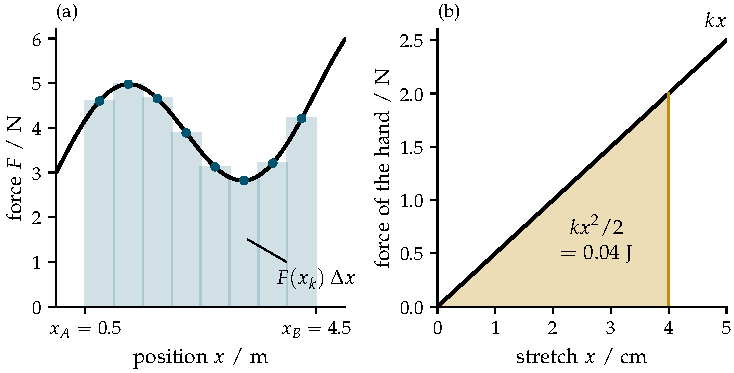
\includegraphics{ch03_energy/area}
\caption{The work of a varying force. (a) A force that changes along the
way; over each short step $\Delta x$ it does about $F(x_k)\,\Delta x$ of
work, the area of a rectangle, and the rectangles add up to the area under
the curve. (b) The force $kx$ that a hand exerts to stretch a spring of
stiffness \SI{50}{\newton\per\metre} slowly; the work to stretch it by
\SI{4}{\centi\metre} is the shaded triangle, $\frac12 kx^2 =
\SI{0.04}{\joule}$.}
\label{fig:en-area}
\end{figure}

\subsection*{Stretching a spring}

A hand that stretches a spring slowly, so that the end of the spring does
not accelerate, must pull with a force equal and opposite to the pull of
the spring, $+kx$ by Hooke's law (\cref{sec:ne-spring}). Stretching from
$x = 0$ to $x$, it does the work
\begin{equation*}
   \int_0^x k x'\,\dd x' = \Bigl[\tfrac12 k x'^2\Bigr]_0^x
   = \tfrac12 k x^2 ,
\end{equation*}
the area of a triangle of base $x$ and height $kx$
(\cref{fig:en-area}b). The variable of integration is written $x'$ to
keep it apart from the upper limit $x$, as in \cref{sec:mo-integrating}.
For the spring of \SI{50}{\newton\per\metre} in \cref{sec:ne-spring},
stretching by \SI{4}{\centi\metre} takes $\frac12\times50\times0.04^2 =
\SI{0.04}{\joule}$. The spring's own force, $-kx$, does the opposite work
when the stretch grows. When its end moves from $x_A$ to $x_B$, by
whatever means,
\begin{equation}
   W_{\mathrm{spring}} = \int_{x_A}^{x_B}(-kx)\,\dd x
   = \Bigl[-\tfrac12 k x^2\Bigr]_{x_A}^{x_B}
   = \tfrac12 k x_A^2 - \tfrac12 k x_B^2 .
   \label{eq:en-spring-work}
\end{equation}

\subsection*{Power}

For a force that varies, we look at the rate at which the kinetic energy
changes, in any number of dimensions. Write $K = \frac12 m(v_x^2 + v_y^2
+ v_z^2)$. By the chain rule of \cref{sec:mo-acceleration}, the rate of
change of $v_x^2$ is $2v_x\,\dd v_x/\dd t = 2v_x a_x$, and likewise for
the other components, so
\begin{align*}
   \frac{\dd K}{\dd t}
   &= \tfrac12 m\,(2v_x a_x + 2v_y a_y + 2v_z a_z)
      && \text{differentiating each square}\\
   &= m\,\vb{a}\cdot\vb{v}
      && \text{the scalar product of \cref{sec:mo-plane}}\\
   &= \vb{F}\cdot\vb{v}
      && \text{by the second law, $m\vb{a} = \vb{F}$,}
\end{align*}
where $\vb{F}$ is the net force. Since $\vb{F}\cdot\vb{v} = \lvert\vb{F}
\rvert\,\lvert\vb{v}\rvert\cos\theta$, with $\theta$ the angle between the
force and the velocity, a net force perpendicular to the velocity leaves
the speed unchanged at that instant and only bends the path. The quantity
$\vb{F}\cdot\vb{v}$ is the rate at which the force does work. Over a short interval $\Delta t$ the
body moves through $\Delta\vb{r} \approx \vb{v}\,\Delta t$, and on so short
a stretch the force is nearly constant, so by
\cref{eq:en-work-constant} it does about $\vb{F}\cdot\vb{v}\,\Delta t$ of
work. The rate at which a force does work is called its power, measured in
joules per second, or watts (\si{\watt}). The trolley pushed by
\SI{10}{\newton} while it moves at \SI{1}{\metre\per\second} receives
\SI{10}{\watt}.

\subsection*{The work-energy theorem}

Integrating the rate of change of $K$ from a time $t_A$ to a time $t_B$,
by \cref{eq:mo-integrals},
\begin{equation}
   K(t_B) - K(t_A) = \int_{t_A}^{t_B}\vb{F}\cdot\vb{v}\,\dd t = W .
   \label{eq:en-work-energy}
\end{equation}
The integral adds up the work $\vb{F}\cdot\vb{v}\,\dd t$ done over every
short interval of the motion, so it is the work done by the net force
along the way the body actually goes. This is the work-energy theorem:
\emph{the change in the kinetic energy of a body equals the work done on
it by the net force}. It holds for any force, constant or varying, and
for any motion; the second law is its only ingredient.

When the motion is along a line and the force depends on position alone,
the integral over time becomes the area of \cref{eq:en-work-line}. Let
$G(x)$ be any function whose derivative is the force, $G'(x) = F(x)$. One
such function is the area $G(x) = \int_{x_A}^{x} F(x')\,\dd x'$, because
moving its upper limit from $x$ to $x + h$ adds a thin strip of area about
$F(x)\,h$, so that $G'(x) = \lim_{h\to0}[G(x+h) - G(x)]/h = F(x)$. This is
the fundamental theorem of calculus (\cref{sec:mo-integrating}) read the
other way: integrating a function and then differentiating returns the
function. Along the motion $x(t)$ the chain
rule gives
\begin{equation*}
   \frac{\dd}{\dd t}\,G\bigl(x(t)\bigr) = G'(x)\,\frac{\dd x}{\dd t}
   = F(x)\,v ,
\end{equation*}
so the integrand $F v$ is the rate of change of $G(x(t))$, and
integrating it from $t_A$ to $t_B$ gives the change in $G$,
\begin{equation*}
   \int_{t_A}^{t_B} F(x)\,v\,\dd t = G(x_B) - G(x_A)
   = \int_{x_A}^{x_B} F(x)\,\dd x ,
\end{equation*}
where $x_A$ and $x_B$ are the positions at the two times. This holds even
if the body goes back and forth on the way, because only the ends enter.

The block of \cref{sec:ne-spring}, of mass \SI{0.5}{\kilogram}, released
from rest \SI{4}{\centi\metre} from its resting place, shows what this
buys. As it moves to $x = 0$ the spring does, by
\cref{eq:en-spring-work}, $\frac12\times50\times0.04^2 - 0 =
\SI{0.04}{\joule}$ of work on it, and the block's kinetic energy grows
from zero to \SI{0.04}{\joule}. Its speed at the centre is therefore
\begin{equation*}
   v = \sqrt{\frac{2\times0.04}{0.5}} = \SI{0.4}{\metre\per\second} ,
\end{equation*}
the largest speed $A\omega$ found in \cref{sec:ne-spring} from the full
solution. The energy argument needed neither the sinusoid nor the time
taken.

\begin{selfcheck}
How much work does it take to stretch the spring of
\SI{50}{\newton\per\metre} from \SI{4}{\centi\metre} to
\SI{8}{\centi\metre}? Why is it more than the work of the first
\SI{4}{\centi\metre}?
\end{selfcheck}

%=============================================================================!
% 3.4  POTENTIAL ENERGY AND THE CONSERVATION OF ENERGY                        !
%=============================================================================!
\section{Potential energy and the conservation of energy}
\label{sec:en-potential}

A ball thrown upwards slows down, stops and falls back, arriving at the
hand with the speed it left with. Its kinetic energy has gone and come
back, as though it had been stored somewhere on the way up. This section
makes the store precise for a position-dependent force along a line, and
shows that Newton's second law then keeps the total fixed.

\subsection*{Potential energy}

The weight of a body and the pull of a spring both depend only on where
the body is, not on how fast it moves or on the time. For such a force
$F(x)$ along a line, \cref{eq:en-work-line} gives the work from $x_A$ to
$x_B$ as an integral fixed by the two ends. Choose a fixed reference
point $x_0$, which need not be where the motion starts, and define the
potential energy
\begin{equation}
   U(x) = -\int_{x_0}^{x} F(x')\,\dd x' ,
   \label{eq:en-potential}
\end{equation}
minus the work the force does as its body moves from $x_0$ to $x$. Two
rules for integrals follow from writing each one, as in
\cref{sec:en-varying}, as the change $G(b) - G(a)$ in a function with $G'
= F$: reversing the limits changes the sign, since $G(a) - G(b) =
-[G(b) - G(a)]$, and an integral can be split at any point $c$, inside the
range or not, since $[G(c) - G(a)] + [G(b) - G(c)] = G(b) - G(a)$. Then,
splitting the integral at $x_0$ and reversing the first part,
\begin{align*}
   W_{A\to B} &= \int_{x_A}^{x_B} F\,\dd x
   = \int_{x_A}^{x_0} F\,\dd x + \int_{x_0}^{x_B} F\,\dd x
      && \text{going by way of $x_0$}\\
   &= -\int_{x_0}^{x_A} F\,\dd x + \int_{x_0}^{x_B} F\,\dd x
      && \text{reversing the first integral}\\
   &= U(x_A) - U(x_B)
      && \text{by \cref{eq:en-potential}.}
\end{align*}
The work done by the force is the drop in potential energy. The force
uses up potential energy when it does positive work, and stores it when
it does negative work, as the weight does while the ball rises.

Moving the reference point from $x_0$ to $x_1$ adds the same constant to
$U$ everywhere, since splitting the integral at $x_0$ gives
$-\int_{x_1}^{x} F\,\dd x' = -\int_{x_1}^{x_0} F\,\dd x' + U(x)$, whose
first term does not depend on $x$; this changes no drop in $U$. Only differences of potential
energy have a physical meaning, and we choose $x_0$ wherever it is
convenient. The force follows from $U$: by the fundamental theorem of
calculus, read as in \cref{sec:en-varying}, the derivative of
$\int_{x_0}^{x}F(x')\,\dd x'$ with respect to its upper limit is $F(x)$,
so
\begin{equation}
   F(x) = -\frac{\dd U}{\dd x} .
   \label{eq:en-force-1d}
\end{equation}
The force points the way $U$ decreases, and the steeper the graph of $U$,
the stronger the force.

Two potential energies follow at once. For a body near the ground, with
$x$ its height measured upwards, the weight is $F = -mg$, and with $x_0 =
0$,
\begin{equation*}
   U(x) = -\int_0^x(-mg)\,\dd x' = mgx .
\end{equation*}
For a spring, $F = -kx$, and with $x_0 = 0$ at the natural length,
\begin{equation*}
   U(x) = -\int_0^x(-kx')\,\dd x' = \tfrac12 k x^2 ,
\end{equation*}
the work of \cref{sec:en-varying} now stored in the stretched spring.

\subsection*{Conservation of energy}

When the net force is of this kind, the work-energy theorem $K_B - K_A = W_{A\to
B}$ and the drop $W_{A\to B} = U_A - U_B$ combine into $K_B - K_A = U_A -
U_B$, or, moving $U_B$ to the left and $K_A$ to the right,
\begin{equation*}
   K_B + U_B = K_A + U_A .
\end{equation*}
The sum of the two energies is the same at every pair of points along the
motion. We call it the total energy, $E = K + U$. The argument can also
be run as a rate, which shows exactly where Newton's law enters.

\begin{proposition}
\label{prop:en-energy-1d}
Let a body of mass $m$ move along a line under a net force $F(x) = -\dd
U/\dd x$ that depends only on its position. Then its total energy
\begin{equation*}
   E = \tfrac12 m v^2 + U(x)
\end{equation*}
keeps the same value throughout the motion.
\end{proposition}

\begin{proof}
Differentiate $E$ along the motion, using the chain rule on each term:
$\frac12 mv^2$ changes at the rate $mv\,\dd v/\dd t$, and $U(x(t))$ at the
rate $(\dd U/\dd x)\,(\dd x/\dd t) = -F v$. Hence
\begin{align*}
   \frac{\dd E}{\dd t} &= m v\,\frac{\dd v}{\dd t} - F v
   = v\,\Bigl(m\,\frac{\dd v}{\dd t} - F\Bigr) = 0 ,
\end{align*}
because the bracket vanishes by the second law, $m\,\dd v/\dd t = F$. A
quantity whose rate of change is zero does not change.
\end{proof}

Newton's second law enters at a single point: it turns the rate of change
of the kinetic energy into the power of the force, which the potential
energy then exactly cancels. Energy is therefore conserved, in the sense
of \cref{sec:ne-bodies}, and \cref{prop:en-energy-1d} is the conservation
of energy. Forces that have a potential energy, and so
conserve $E$, are called conservative.

\subsection*{Two checks}

Energy reproduces the results of the earlier chapters with no equation
of motion solved. A ball of \SI{0.5}{\kilogram} thrown up at
\SI{12}{\metre\per\second} starts at $x = 0$, where $U = 0$, with $E = K =
\frac12\times0.5\times12^2 = \SI{36}{\joule}$. At the top of its flight
$K = 0$, so all of $E$ is potential energy, $mgx_{\max} = E$, and
\begin{equation*}
   x_{\max} = \frac{E}{mg} = \frac{36}{0.5\times9.80665}
   = \SI{7.342}{\metre} ,
\end{equation*}
the height found in \cref{sec:mo-integrating}. Halfway up, at
\SI{3.671}{\metre}, $U = mgx$ is half its value at the top, so half of $E$
is potential energy and half kinetic: $\frac12 mv^2 = \SI{18}{\joule}$,
half the kinetic energy of the throw, so $v^2$ is half of $12^2$ and $v =
12/\sqrt2 = \SI{8.485}{\metre\per\second}$. \Cref{fig:en-ball} follows $K$ and $U$
through the flight: they trade with each other while their sum stays at
\SI{36}{\joule}. Plotted against height, $U = mgx$ is a straight line and
so is $K = E - mgx$, which reaches zero exactly at the top.

For the block on a spring, at a turning point $x = \pm A$ the block is at
rest and $E = \frac12 kA^2$; at the centre $U = 0$ is at its smallest, so
$K = E - U$ and the speed are at their largest, and $E = \frac12
mv_{\max}^2$. Equating the two,
\begin{equation*}
   \tfrac12 m v_{\max}^2 = \tfrac12 k A^2
   \quad\Longrightarrow\quad
   v_{\max} = A\sqrt{\frac{k}{m}} = A\omega ,
\end{equation*}
with $\omega$ from \cref{eq:ne-spring-omega}, as in \cref{sec:ne-spring}.

\begin{figure}[htb]
\centering
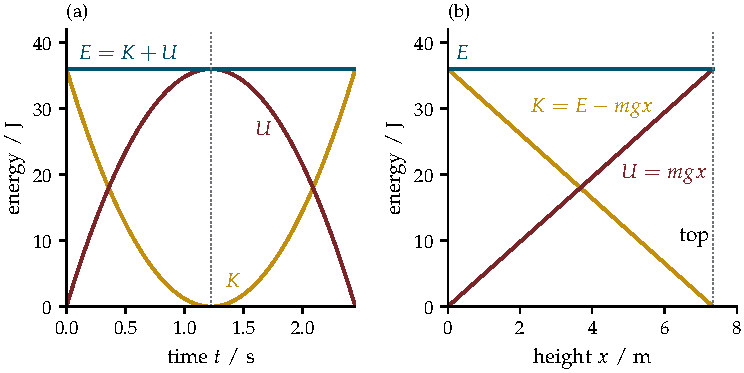
\includegraphics{ch03_energy/ball}
\caption{The energies of a ball of \SI{0.5}{\kilogram} thrown straight up
at \SI{12}{\metre\per\second}. (a) Kinetic energy $K$, potential energy
$U = mgx$ and their sum $E$ against time; the dotted line marks the top.
(b) The same against height: $K$ and $U$ are straight lines, and $K$
reaches zero at the top, \SI{7.342}{\metre}.}
\label{fig:en-ball}
\end{figure}

\begin{keyidea}
A force that depends only on position along a line has a potential energy
$U(x) = -\int_{x_0}^{x} F(x')\,\dd x'$, with $F = -\dd U/\dd x$. Newton's second law then
keeps the total energy $E = K + U$ constant: kinetic and potential energy
are traded, never their sum.
\end{keyidea}

\notebook{03}{follow $K$, $U$ and $E$ through the throw with a time
cursor}

\begin{selfcheck}
A ball is thrown at \SI{12}{\metre\per\second} from a balcony
\SI{5}{\metre} above the ground. With what speed does it reach the
ground? Does the answer depend on whether it is thrown upwards, sideways
or downwards?
\end{selfcheck}

%=============================================================================!
% 3.5  SLIDING ON A HILL-SHAPED TRACK                                         !
%=============================================================================!
\section{Sliding on a hill-shaped track}
\label{sec:en-track}

A ball thrown upwards moves along a straight line. Many motions follow a
curved track instead, as a sledge follows the slopes of a hillside, and
energy is most useful there, because the forces along a curved track
change from point to point. This section treats an object sliding along a
track shaped into hills and valleys, and finds its speed at every point
from its height alone.

\subsection*{A bead on a wire}

The cleanest version of such a track is a smooth, stiff wire bent into
hills and valleys in a vertical plane, with a bead threaded on it. We
measure $x$ horizontally and $y$ vertically upwards, and describe the
shape of the wire by its height $h(x)$ above the ground; our example,
drawn in \cref{fig:en-track}(a) in the next section, is
\begin{equation}
   h(x) = 0.15\,x^4 - 0.6\,x^2 + 0.15\,x + 1.0 ,
   \label{eq:en-track}
\end{equation}
with $x$ and $h$ in metres. It has a deep valley on the left, a hill in
the middle and a shallower valley on the right. Three features of this
system are chosen so that it obeys the simple laws below, and each is an
idealisation that a real track only approaches.
\begin{itemize}
\item The bead is threaded on the wire, so it cannot leave the track. A
   block sliding on top of a track could lose contact over a crest, where
   the track curves downwards more sharply than the fast-moving block can
   follow, and then fly through the air instead.
\item The bead slides. A ball rolling along a track also spins, and part
   of its kinetic energy is then in the spinning, so at each height a
   rolling ball moves more slowly than a sliding body; Chapter~5 treats
   spinning.
\item The wire is smooth. No real wire is perfectly smooth: friction
   slowly removes energy (\cref{sec:en-friction}), and a real bead never
   quite returns to the height from which it was released.
\end{itemize}

\subsection*{The push of the wire does no work}

Two forces act on the bead: its weight, $m\vb{g}$ downwards, and the
push of the wire. A smooth surface exerts no friction, so the push of the
wire has no component along the wire: it is a normal force,
perpendicular to the wire at the point where the bead is
(\cref{fig:en-bead}a). Its size and direction change as the bead moves,
and we do not need to know them. The velocity of the bead points along
its path (\cref{sec:mo-plane}), which is along the wire, so the normal
force $\vb{F}_{\mathrm{n}}$ is perpendicular to the velocity at every
instant, $\vb{F}_{\mathrm{n}}\cdot\vb{v} = 0$. Its power is therefore
zero throughout, so the work it does over any part of the motion, the
integral of its power as in \cref{eq:en-work-energy}, is zero.

\begin{figure}[htb]
\centering
\begin{tikzpicture}[line cap=round, line join=round, scale=1.3,
   force/.style={-{Stealth[length=5pt]}, line width=1.0pt}]
   % (a) the forces on the bead
   \begin{scope}
      \node at (0.1,2.25) {\small (a)};
      \draw[line width=0.9pt, black!70, domain=0:3.6, smooth, samples=60]
         plot (\x, {1.1 + 0.55*cos(deg(1.3*\x)) + 0.05*\x});
      \coordinate (P) at (1.6,0.912);
      \draw[force] (P) -- ++(0.498*0.95, 0.867*0.95)
         node[above] {\small $\vb{F}_{\mathrm{n}}$};
      \draw[force] (P) -- ++(0,-0.95) node[below] {\small $m\vb{g}$};
      \draw[force, accent, dashed] (P) -- ++(0.867*0.9, -0.498*0.9)
         node[right] {\small $\vb{v}$};
      \fill[black!15, draw=black, line width=0.5pt] (P) circle (0.09);
   \end{scope}
   % (b) the wire cut into short chords
   \begin{scope}[xshift=4.3cm]
      \node at (0.1,2.25) {\small (b)};
      \draw[line width=0.5pt, black!35, domain=0:5.0, smooth, samples=60]
         plot (\x, {1.1 + 0.55*cos(deg(1.3*\x)) + 0.05*\x});
      \draw[line width=0.8pt, accent] (0.2,1.642) -- (1.1,1.232)
         -- (2.0,0.729) -- (2.9,0.800) -- (3.8,1.414) -- (4.7,1.877);
      \foreach \x/\y in {0.2/1.642, 1.1/1.232, 2.0/0.729, 2.9/0.800,
         3.8/1.414, 4.7/1.877}
         \fill[accent] (\x,\y) circle (1.3pt);
      \draw[black!60, dashed, line width=0.4pt] (2.9,0.800) -- (3.8,0.800);
      \draw[{Stealth[length=3pt]}-{Stealth[length=3pt]}, line width=0.4pt]
         (2.9,0.62) -- (3.8,0.62) node[midway, below] {\small $\Delta x_k$};
      \draw[{Stealth[length=3pt]}-{Stealth[length=3pt]}, line width=0.4pt]
         (3.95,0.800) -- (3.95,1.414) node[midway, right] {\small $\Delta y_k$};
      \node[below] at (0.2,1.58) {\small $A$};
      \node[above] at (4.7,1.95) {\small $B$};
   \end{scope}
\end{tikzpicture}
\caption{A bead on a smooth wire. (a) The two forces on the bead: its
weight $m\vb{g}$ and the push $\vb{F}_{\mathrm{n}}$ of the wire, which is
perpendicular to the wire and so to the velocity $\vb{v}$. (b) The wire
from $A$ to $B$ replaced by short straight chords; on the chord that
rises by $\Delta y_k$ the weight does the work $-mg\,\Delta y_k$.}
\label{fig:en-bead}
\end{figure}

\subsection*{The work of the weight}

The weight is constant, but the path is curved. To extend the straight-path
argument of \cref{eq:en-work-constant}, we replace the wire between two
points $A$ and $B$ by a chain of short straight chords
(\cref{fig:en-bead}b). On the $k$th chord the displacement is $(\Delta
x_k, \Delta y_k)$, and the weight, $(0, -mg)$, does the work
\begin{equation*}
   (0, -mg)\cdot(\Delta x_k, \Delta y_k) = -mg\,\Delta y_k .
\end{equation*}
Adding the chords, the rises $\Delta y_k$ add up to the total rise from
$A$ to $B$, since each chord starts where the one before it ends, so
\begin{equation*}
   W_{\mathrm{weight}} = -mg\sum_k\Delta y_k = -mg\,(y_B - y_A) .
\end{equation*}
The result is the same for any number of chords, so it holds also in the
limit in which the chords follow the wire exactly. The weight does work
that depends only on the change in height, whatever the shape of the path
between.

\subsection*{The speed at every height}

By the work-energy theorem \cref{eq:en-work-energy}, the change in the
bead's kinetic energy is the work of the weight plus the work of the
wire, $-mg\,(y_B - y_A) + 0$. On the wire $y = h(x)$, so
\begin{align*}
   \tfrac12 m v_B^2 - \tfrac12 m v_A^2
   &= -mg\,\bigl(h(x_B) - h(x_A)\bigr)\\
   &= -mg\,h(x_B) + mg\,h(x_A)
      && \text{multiplying out the bracket,}\\
   \tfrac12 m v_B^2 + mg\,h(x_B) &= \tfrac12 m v_A^2 + mg\,h(x_A)
      && \text{adding $mg\,h(x_B) + \tfrac12 m v_A^2$ to both sides.}
\end{align*}
The total energy
\begin{equation}
   E = \tfrac12 m v^2 + mg\,h(x)
   \label{eq:en-track-energy}
\end{equation}
is conserved, with the potential energy $U = mgh(x)$ of the weight. It is
convenient to write $E = mgh_E$, so that $h_E$ is the height at which the bead
would be at rest; a bead released from rest at height $h_E$ has exactly
this energy. Then $\frac12 mv^2 = mg\,(h_E - h)$, and dividing by $m/2$ and
taking the square root,
\begin{equation*}
   v = \sqrt{2g\,\bigl(h_E - h(x)\bigr)} .
\end{equation*}
The mass has cancelled: every bead released from the same height moves
at the same speed at the same place. Released from rest at $h_E =
\SI{1.3}{\metre}$, the bead passes the bottom of the deep valley, where
$h = \SI{0.1834}{\metre}$, at $\sqrt{2\times9.80665\times(1.3 - 0.1834)} =
\SI{4.680}{\metre\per\second}$, crosses the top of the hill, at
\SI{1.0094}{\metre}, at \SI{2.387}{\metre\per\second}, and passes the
bottom of the shallow valley, at \SI{0.6072}{\metre}, at
\SI{3.686}{\metre\per\second}. None of these numbers required the shape
of the wire between the points, or the time taken to get there.

Energy gives the speed at each place directly. It does not say which way
the bead is moving: a bead passing a point to the left and one passing it
to the right have the same speed. Nor does it give the time of arrival at
once; that needs the time spent on each short stretch of wire, its length
divided by the speed there, added up along the way, or the equation of
motion along the wire, which Chapter~6 derives in a form suited to such
constrained motion.

\notebook{03}{release the bead from different heights and read its speed}

\begin{selfcheck}
A bead is released from rest on the left slope at a height of
\SI{0.8}{\metre}. Can it reach the shallow valley on the right? What is
the least speed it would need at the bottom of the deep valley to cross
the hill?
\end{selfcheck}

%=============================================================================!
% 3.6  ENERGY DIAGRAMS                                                        !
%=============================================================================!
\section{Energy diagrams}
\label{sec:en-diagrams}

The conservation of energy turns a graph of the potential energy into a
map of every possible motion. This section reads such a map.

\subsection*{Allowed regions and turning points}

For a body moving along a line with potential energy $U(x)$, or a bead on
a wire with $U = mgh(x)$, the kinetic energy at each point is what
remains of the total, $K = E - U(x)$. A kinetic energy $\frac12 mv^2$
cannot be negative, so the body can only be where
\begin{equation*}
   U(x) \le E .
\end{equation*}
These points form the allowed region of the motion. Where $U$ rises to
meet $E$, the kinetic energy falls to zero, the body stops for an
instant, and the force, which points down the slope of $U$ by
\cref{eq:en-force-1d} (for the bead, the part of the weight along the
wire, which points downhill), sends it back the way it came. Such a point, where
$U(x) = E$ with a non-zero slope of $U$, is a turning point. If $E$ instead
meets $U$ at an equilibrium, the force also vanishes there: a body placed
there at rest stays there, and approaching an unstable equilibrium can
take indefinitely long. Away from these special points, the speed follows
from $\frac12 mv^2 = E - U(x)$,
\begin{equation*}
   v = \sqrt{\frac{2\,\bigl(E - U(x)\bigr)}{m}} .
\end{equation*}

A graph of $U$ with a horizontal line at the height $E$ is called an
energy diagram. For the bead, $U/mg = h$ is the shape of the wire itself,
so its energy diagram is a picture of the track, and $E/mg = h_E$ is the
height at which the bead would be at rest. \Cref{fig:en-track}(a) draws
three energies. Their turning points, the solutions of $h(x) = h_E$, were
found by computer; substituting them into \cref{eq:en-track} checks them,
and two are exact, $h(-1) = 0.4$ and $h(2) = 1.3$.
\begin{itemize}
\item At $h_E = \SI{0.4}{\metre}$ the bead is confined to the deep valley,
   between the turning points $x = \SI{-1.831}{\metre}$ and
   \SI{-1.000}{\metre}. It slides back and forth between them for ever.
\item At $h_E = \SI{0.8}{\metre}$ there are two separate allowed regions,
   one in each valley: from \num{-2.042} to \SI{-0.477}{\metre}, and from
   \num{0.795} to \SI{1.724}{\metre}. With the same energy the bead may
   be in either, but it cannot cross the hill between them, which rises to
   \SI{1.009}{\metre}. Which valley it occupies depends only on where it
   started.
\item At $h_E = \SI{1.3}{\metre}$ the bead passes over the hill and turns
   only at the steep ends of the track, at \num{-2.206} and
   \SI{2.000}{\metre}.
\end{itemize}
\Cref{fig:en-track}(b) gives the speed along the track at the highest of
these energies. It falls to zero at the turning points, is greatest at the
bottom of the deep valley, \SI{4.680}{\metre\per\second}, and dips to
\SI{2.387}{\metre\per\second} as the bead crosses the hill.

\begin{figure}[tb]
\centering
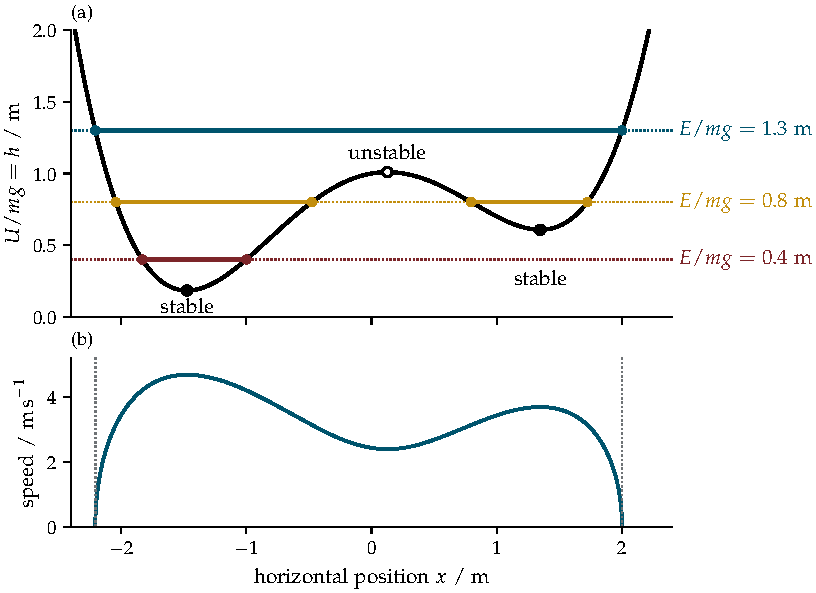
\includegraphics{ch03_energy/track}
\caption{The track as an energy diagram. (a) The potential energy of the
bead divided by $mg$, which is the height $h(x)$ of the wire, with three
total energies $E/mg$. Each energy line is
solid where the bead may be ($U \le E$) and dotted where it may not; dots
mark the turning points. Filled circles mark the stable equilibria at the
valley bottoms, and the open circle the unstable one at the top of the
hill. (b) The speed along the track at $E/mg = \SI{1.3}{\metre}$; the
dotted lines are the turning points.}
\label{fig:en-track}
\end{figure}

\subsection*{Equilibria}

A body placed at rest stays at rest only where the net force on it is
zero. By
\cref{eq:en-force-1d} these are the points where $\dd U/\dd x = 0$, where
the graph of $U$ is flat: the bottoms of valleys, the tops of hills, and
any level shelf. Such a point $x_0$ is called an equilibrium. For the
bead, the push of the wire and the weight balance where the wire is
horizontal, $\dd h/\dd x = 0$, since only there is the push, which is
perpendicular to the wire, vertical, so that it can cancel the weight. Differentiating \cref{eq:en-track} with the
power rule,
\begin{equation*}
   \frac{\dd h}{\dd x} = 0.6\,x^3 - 1.2\,x + 0.15 ,
\end{equation*}
and this cubic is zero at three points, which a computer finds to be $x =
\SI{-1.473}{\metre}$ (the deep valley, $h = \SI{0.183}{\metre}$), $x =
\SI{0.126}{\metre}$ (the hill, $h = \SI{1.009}{\metre}$) and $x =
\SI{1.347}{\metre}$ (the shallow valley, $h = \SI{0.607}{\metre}$).

The equilibria differ in what happens after a small nudge. At the bottom
of a valley, the slope of $U$ on either side points back down into the
valley, so the force on a displaced body points back towards the
equilibrium, and the body swings about it: the equilibrium is stable. At
the top of a hill, the slope on either side leads away, and a body nudged
off it runs away down one side: the equilibrium is unstable.

The second derivative of $U$ tells the two apart without a picture. Near
an equilibrium $x_0$, the Taylor series of \cref{sec:mo-taylor}, applied
to the force $F$ about $x_0$ with $x - x_0$ in the role of the interval
$\tau$, gives
\begin{align*}
   F(x) &= F(x_0) + F'(x_0)\,(x - x_0) + \order{(x - x_0)^2}\\
   &= -U''(x_0)\,(x - x_0) + \order{(x - x_0)^2}
      && \text{since $F(x_0) = 0$ and $F' = -U''$,}
\end{align*}
where $U''$ is the second derivative of $U$ with respect to $x$. If
$U''(x_0) > 0$, the graph of $U$ curves upwards, as at a valley bottom,
and close to $x_0$ the force is that of a spring of stiffness $k =
U''(x_0)$, $F \approx -k\,(x - x_0)$: it always points back, the
equilibrium is stable. By \cref{sec:ne-spring}, with the displacement
$x - x_0$ in place of $x$, the body then oscillates about $x_0$,
approximately, with angular frequency $\sqrt{U''(x_0)/m}$,
and Chapter~4 examines how good the approximation is. If $U''(x_0) <
0$, the force points away on both sides, and the equilibrium is unstable.
If $U''(x_0) = 0$, the next terms of the series decide. For the track,
$\dd^2 h/\dd x^2 = 1.8\,x^2 - 1.2$, which is \SI{+2.706}{\per\metre} and
\SI{+2.066}{\per\metre} at the two valley bottoms and
\SI{-1.171}{\per\metre} at the top of the hill, as the picture says.

\notebook{03}{move $E$ on the energy diagram and watch the allowed regions
change}

\begin{selfcheck}
At $E/mg = \SI{0.8}{\metre}$ a bead starts at rest at $x =
\SI{0.795}{\metre}$. Where does it next turn back, where is it fastest,
and how fast is it moving there?
\end{selfcheck}

%=============================================================================!
% 3.7  FRICTION AND THE LOSS OF ENERGY                                        !
%=============================================================================!
\section{Friction and the loss of energy}
\label{sec:en-friction}

A box shoved across a floor slides to a stop, and a real bead on a real
wire never quite climbs back to the height it was released from. Both
lose energy to friction. This section measures the loss and finds the
rule that says how fast the total energy changes when part of the force
is not conservative.

\subsection*{Sliding friction}

When one surface slides over another, each exerts on the other a
friction force along the surfaces, and the force on each points against
the direction in which that surface slides over the other. For many pairs of dry surfaces, the size of this force depends only
weakly on the speed and on the area in contact, and is roughly
proportional to the normal force $F_{\mathrm{n}}$ with which the surfaces
are pressed together,
\begin{equation*}
   F_{\mathrm{fr}} = \mu_{\mathrm{k}}\,F_{\mathrm{n}} .
\end{equation*}
The number $\mu_{\mathrm{k}}$, the coefficient of sliding friction,
depends on the two surfaces and is found by measurement. This rule is an empirical description of limited
accuracy, and we use it only to see how energy is lost.

A box of \SI{5}{\kilogram} slides across a level floor at
\SI{2}{\metre\per\second}, with $\mu_{\mathrm{k}} = 0.3$. Vertically the
box does not accelerate, so the normal force balances the weight,
$F_{\mathrm{n}} = mg$, and the friction is $0.3\times5\times9.80665 =
\SI{14.71}{\newton}$, pointing against the motion. The weight and the
normal force are perpendicular to the motion and do no work, so over a
distance $d$ the work on the box is that of friction, $-\mu_{\mathrm{k}}
mg\,d$. The box stops when this has removed all of its kinetic energy,
\begin{align*}
   0 - \tfrac12 m v_0^2 &= -\mu_{\mathrm{k}} m g\,d ,\\
   d &= \frac{v_0^2}{2\mu_{\mathrm{k}}g}
      && \text{dividing both sides by $-\mu_{\mathrm{k}}mg$}\\
   &= \frac{2^2}{2\times0.3\times9.80665} = \SI{0.680}{\metre} .
\end{align*}
The mass cancels again: a heavier box has proportionally more kinetic
energy to lose, and it presses harder on the floor and feels a
proportionally larger friction.

The \SI{10}{\joule} of kinetic energy the box had is not destroyed. The
rubbing surfaces warm up, and Chapter~12 shows that warmth is the hidden
kinetic and potential energy of the jiggling atoms of the box and the
floor. Energy has passed from the motion of the box as a whole, which we
follow, into motions of its atoms, which we do not.

\subsection*{Down a rough ramp}

A block of \SI{2}{\kilogram} slides from rest down a straight ramp
\SI{3}{\metre} long, inclined at \ang{30}, with $\mu_{\mathrm{k}} = 0.2$
(\cref{fig:en-ramp}). Three forces act. The line perpendicular to the
ramp is the vertical turned through the same \ang{30} as the ramp is
turned from the level, so it makes an angle of \ang{30} with the weight,
$mg$ straight down. As for the sledge of \cref{sec:en-constant}, the
weight therefore has a component $mg\cos\ang{30}$ into the ramp and a
component $mg\sin\ang{30}$ at right angles to that, down the ramp. The
normal force balances the first of these, because the block does not
accelerate into or away from the ramp, so $F_{\mathrm{n}} = mg\cos\ang{30}
= \SI{16.986}{\newton}$. Friction acts up the ramp with size
$\mu_{\mathrm{k}}F_{\mathrm{n}} = 0.2\times16.986 = \SI{3.397}{\newton}$.

\begin{figure}[htb]
\centering
\begin{tikzpicture}[line cap=round, line join=round, scale=1.15,
   force/.style={-{Stealth[length=5pt]}, line width=1.0pt},
   part/.style={-{Stealth[length=4pt]}, line width=0.6pt, dashed}]
   % the ramp, rising to the left at 30 degrees
   \fill[black!10] (0,0) -- (5.2,0) -- (0,3.0) -- cycle;
   \draw[line width=0.6pt] (0,0) -- (5.2,0) -- (0,3.0);
   \draw[black!50, line width=0.4pt] (4.3,0) arc[start angle=180,
      end angle=150, radius=0.9];
   \node at (3.95,0.2) {\small \ang{30}};
   % the block, its centre on the line through the middle of its face
   \begin{scope}[shift={(2.25,1.70)}, rotate=-30]
      \draw[line width=0.6pt, fill=white] (-0.45,0) rectangle (0.45,0.6);
      \coordinate (C) at (0,0.3);
   \end{scope}
   % weight and its two parts
   \draw[force] (C) -- ++(0,-1.35) coordinate (W)
      node[below] {\small $mg$};
   \draw[part] (C) -- ++(-30:0.675) node[right] {\small $mg\sin\ang{30}$};
   \draw[part] (C) -- ++(-120:1.169) node[below left] {\small $mg\cos\ang{30}$};
   % normal force and friction
   \draw[force, accent] (C) -- ++(60:1.169) node[above right]
      {\small $F_{\mathrm{n}}$};
   \draw[force, oxblood] ($(C)+(150:0.45)$) -- ++(150:0.234)
      node[above left] {\small $F_{\mathrm{fr}}$};
   \draw[black!50, line width=0.4pt] ($(C)+(-90:0.5)$) arc[start angle=-90,
      end angle=-120, radius=0.5];
   \node at ($(C)+(-105:0.72)$) {\scriptsize \ang{30}};
   \fill (C) circle (1.3pt);
\end{tikzpicture}
\caption{A block sliding down a rough ramp. Its weight $mg$ is split
(dashed) into a part along the ramp and a part into it. The normal force
$F_{\mathrm{n}}$ (teal) balances the part into the ramp, and friction
$F_{\mathrm{fr}}$ (dark red) acts up the ramp, against the motion.}
\label{fig:en-ramp}
\end{figure}

Over the length $L = \SI{3}{\metre}$ the block drops by $L\sin\ang{30} =
\SI{1.5}{\metre}$, and the three forces do the work
\begin{align*}
   W_{\mathrm{weight}} &= -mg\times(-1.5)
      && \text{by \cref{sec:en-track}, $-mg$ times the rise,}\\
   &= 2\times9.80665\times1.5 = \SI{29.42}{\joule} ,\\
   W_{\mathrm{n}} &= 0
      && \text{perpendicular to the motion,}\\
   W_{\mathrm{fr}} &= -3.397\times3 = \SI{-10.19}{\joule}
      && \text{against the motion.}
\end{align*}
The block arrives with $K = 29.42 - 10.19 = \SI{19.23}{\joule}$, and so
with speed $\sqrt{2\times19.23/2} = \SI{4.385}{\metre\per\second}$; on a
smooth ramp it would arrive at $\sqrt{2g\times1.5} =
\SI{5.424}{\metre\per\second}$.

\subsection*{The rate of energy loss}

Friction and the drag of \cref{sec:ne-drag} always point against the
velocity, so on a trip out to a point and back they do negative work on
both legs, whereas a force with a potential energy does the work $U(x_A)
- U(x_A) = 0$ on any trip that returns to its start $x_A$. They therefore
have no potential energy. To see their effect on $E$, write the net force
on a body moving along a line as a conservative part, $-\dd U/\dd x$,
plus the rest, $F^{\mathrm{nc}}$, the non-conservative part. The kinetic
energy changes at the rate $(-\dd U/\dd x + F^{\mathrm{nc}})\,v$, by
\cref{sec:en-varying}, and the potential energy at the rate $(\dd U/\dd
x)\,v$, by the chain rule, so their sum changes at the rate
\begin{equation}
   \frac{\dd E}{\dd t} = F^{\mathrm{nc}}\,v :
   \label{eq:en-dEdt-1d}
\end{equation}
the total energy changes at exactly the rate at which the
non-conservative force does work. Friction always opposes the velocity,
so $F^{\mathrm{nc}}v = -\mu_{\mathrm{k}}F_{\mathrm{n}}\lvert v\rvert$, and
the energy can only fall. For linear drag, $F^{\mathrm{nc}} = -bv$ and
$\dd E/\dd t = -bv^2$.

The bead of \cref{sec:ne-drag} sinking at its terminal velocity shows
this rate at work. Measuring the depth $x$ downwards, its potential
energy is $U = -mgx$, which falls at the rate $mg\,v_\infty$, while its
kinetic energy stays constant. Every second, then, the weight does
$mg\,v_\infty = 0.01\times9.80665\times1.961 = \SI{0.1923}{\joule}$ of
work, and the drag removes all of it: $bv_\infty^2 = 0.05\times1.961^2 =
\SI{0.1923}{\watt}$, the same, because $bv_\infty = mg$.

\begin{selfcheck}
A box sliding across a floor stops after \SI{0.68}{\metre}. How far would
a box of twice the mass, sliding on the same floor at the same starting
speed, travel before stopping? Where has the kinetic energy gone?
\end{selfcheck}

%=============================================================================!
% 3.8  THE ENERGY OF SEVERAL BODIES                                           !
%=============================================================================!
\section{The energy of several bodies}
\label{sec:en-bodies}

\Cref{sec:ne-bodies} showed that the forces two bodies exert on each
other cannot change their total momentum. This section asks the same
question of energy, using the two carts of that section, and finds a
different answer: forces between bodies can change their total kinetic
energy, and they conserve the total energy only when they store what they
give in a potential energy.

\subsection*{The pair of forces does work}

Two carts, of masses $m_1 = \SI{1}{\kilogram}$ and $m_2 =
\SI{3}{\kilogram}$, at positions $x_1 < x_2$ on a level, smooth track,
are pushed apart by a light spring of stiffness $k =
\SI{200}{\newton\per\metre}$ compressed between them
(\cref{fig:ne-carts-sketch}). Let $\xi$ be the compression of the spring,
how much shorter it is than its natural length. The spring touches both
carts, so as the gap $x_2 - x_1$ between them grows, $\xi$ shrinks by the
same amount:
\begin{equation*}
   \frac{\dd \xi}{\dd t} = -\frac{\dd}{\dd t}(x_2 - x_1) = -(v_2 - v_1) .
\end{equation*}
By \cref{sec:ne-bodies} the spring pushes the two carts with forces of
equal size in opposite directions, and by Hooke's law
(\cref{sec:ne-spring}) a spring compressed by $\xi$ pushes with a force of
size $k\xi$, so it pushes the first cart with $-k\xi$ and the second with
$+k\xi$. The weights and normal forces do no work, so by \cref{sec:en-varying} the kinetic energies change at the rates
\begin{equation*}
   \frac{\dd K_1}{\dd t} = -k\xi\,v_1 , \qquad
   \frac{\dd K_2}{\dd t} = +k\xi\,v_2 .
\end{equation*}
Adding them,
\begin{align*}
   \frac{\dd}{\dd t}\bigl(K_1 + K_2\bigr) &= k\xi\,(v_2 - v_1)\\
   &= -k\xi\,\frac{\dd \xi}{\dd t}
      && \text{using the rate of change of $\xi$}\\
   &= -\frac{\dd}{\dd t}\bigl(\tfrac12 k\xi^2\bigr)
      && \text{since $\tfrac{\dd}{\dd t}\bigl(\tfrac12 k\xi^2\bigr)
         = k\xi\,\tfrac{\dd \xi}{\dd t}$ by the chain rule.}
\end{align*}
Moving the last term to the left, the sum
\begin{equation*}
   E = \tfrac12 m_1 v_1^2 + \tfrac12 m_2 v_2^2 + \tfrac12 k \xi^2
\end{equation*}
does not change: the total energy of the two carts and the spring is
conserved, and $\frac12 k\xi^2$ is the potential energy of the spring, as in
\cref{sec:en-potential}. It depends only on how far apart the carts are.

The contrast with momentum lies in the velocities. The two forces are
equal and opposite, so they cancel in the total momentum, whose rate of
change is their sum. Their powers are $-k\xi\,v_1$ and $+k\xi\,v_2$, which
cancel only if $v_1 = v_2$. When the carts move apart, the first moves
backwards, along its push, and the second forwards, along its push, so
both forces do positive work and the total kinetic energy grows. A pair
of equal and opposite forces does work whenever the distance between the
bodies changes. This is how the carts, at rest at first, come to move.

\subsection*{The speeds of the carts}

The spring starts compressed by \SI{0.1}{\metre}, so it stores $\frac12
\times200\times0.1^2 = \SI{1}{\joule}$, and the carts start at rest. Once
the spring has reached its natural length and fallen away, $\xi = 0$ and
all of that energy is kinetic,
\begin{equation*}
   \tfrac12 m_1 v_1^2 + \tfrac12 m_2 v_2^2 = \SI{1}{\joule} .
\end{equation*}
One equation cannot fix two speeds, but momentum supplies the second. The
total momentum stays zero (\cref{sec:ne-bodies}), so $m_1 v_1 + m_2 v_2
= 0$, which gives $v_1 = -(m_2/m_1)\,v_2 = -3v_2$. Substituting,
\begin{equation*}
   \tfrac12\times1\times(-3v_2)^2 + \tfrac12\times3\times v_2^2
   = \tfrac92 v_2^2 + \tfrac32 v_2^2 = 6\,v_2^2 = 1 ,
\end{equation*}
in joules, so $v_2^2 = \frac16$ and
\begin{equation*}
   v_2 = +\sqrt{\tfrac16} = +\SI{0.408}{\metre\per\second} , \qquad
   v_1 = -3\sqrt{\tfrac16} = -\SI{1.225}{\metre\per\second} ,
\end{equation*}
taking the positive root for $v_2$ because the spring pushes the second
cart forwards. These are the speeds that a computer solution of the
equations of motion gave in \cref{sec:ne-bodies}, found now with two
lines of algebra. \Cref{fig:en-carts} shows the energy passing from the
spring to the carts while the total stays at \SI{1}{\joule}.

\begin{figure}[htb]
\centering
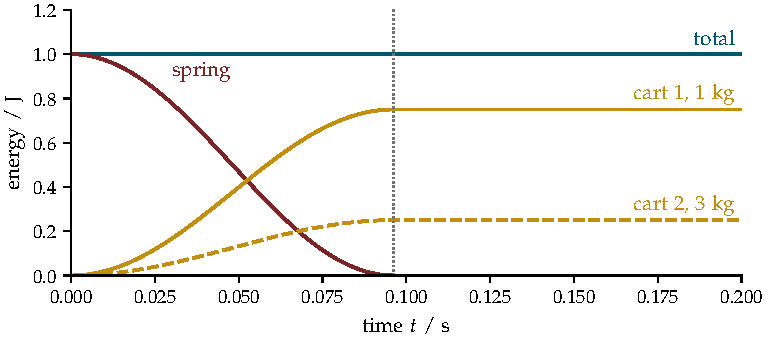
\includegraphics{ch03_energy/carts}
\caption{The energies of the carts of \cref{fig:ne-carts}: the energy
stored in the spring, $\frac12 k\xi^2$, the kinetic energies of the two
carts, and the total, which stays at \SI{1}{\joule}. The spring falls away
at the dotted line, after \SI{0.096}{\second}.}
\label{fig:en-carts}
\end{figure}

The lighter cart ends with \SI{0.75}{\joule} and the heavier with
\SI{0.25}{\joule}, although their momenta are equal and opposite. Writing
the kinetic energy in terms of the momentum $p = mv$ shows why,
\begin{equation*}
   K = \tfrac12 m v^2 = \frac{(mv)^2}{2m} = \frac{p^2}{2m} :
\end{equation*}
for momenta of equal size the kinetic energies are in the inverse ratio of
the masses, three to one here.

The same argument extends to any number of bodies that push on one
another in third-law pairs, provided that the two forces of each pair
act along the line joining its two bodies, with a size that depends only
on the distance between them: each pair then has a potential energy, and the kinetic energy plus the sum of the pair energies
is conserved. \Cref{sec:en-atoms} proves this for atoms, in three
dimensions.

\notebook{03}{change the masses of the carts and the energy they share}

\begin{selfcheck}
If both carts had a mass of \SI{2}{\kilogram}, with the same spring and
compression, at what speeds would they separate?
\end{selfcheck}

%=============================================================================!
% 3.9  WORK ALONG A PATH IN SPACE                                             !
%=============================================================================!
\section{Work along a path in space}
\label{sec:en-paths}

On a line, every force that depends only on position has a potential
energy, because the integral of \cref{eq:en-potential} can always be
done. In a plane or in space a body can travel from one point to another
by many routes, and the work may differ from route to route. This section
defines the work along a curved path, the tool we need, and shows that
the route can matter.

\subsection*{The line integral}

\Cref{sec:en-track} found the work of the weight along a curved wire by
cutting the wire into short straight chords. The same construction works
for any force, constant or not, and the box below turns it into a
definition.

\begin{toolbox}[Line integrals]
Let a path $C$ run from a point $A$ to a point $B$, and let a force
$\vb{F}(\vb{r})$ depend on position. Mark points $\vb{r}_0 = A$,
$\vb{r}_1, \dots, \vb{r}_n = B$ in order along the path, and join each to
the next by a straight chord, $\Delta\vb{r}_k = \vb{r}_k -
\vb{r}_{k-1}$. On a chord short enough that the force hardly changes
along it, the force does about $\vb{F}(\bar{\vb{r}}_k)\cdot\Delta
\vb{r}_k$ of work by \cref{eq:en-work-constant}, where $\bar{\vb{r}}_k =
\frac12(\vb{r}_{k-1} + \vb{r}_k)$ is the midpoint of the chord. The work
along the path is the limit of the sum as the chords shrink,
\begin{equation*}
   W[C] = \lim\sum_{k=1}^{n}\vb{F}(\bar{\vb{r}}_k)\cdot\Delta\vb{r}_k
   = \int_C \vb{F}\cdot\dd\vb{r} ,
\end{equation*}
called the line integral of $\vb{F}$ along $C$; the square brackets in
$W[C]$ record that the work belongs to the whole path $C$.
Three properties follow from the sum. Reversing the direction of travel
reverses every chord, $\Delta\vb{r}_k \to -\Delta\vb{r}_k$, and so changes
the sign of the work. The sum uses only the points of the path and their
order, so it does not matter how fast the path is traversed. And along a
path made of one path followed by another, the work is the sum of the
works along the two, since the sum over chords splits into two such sums.
For a closed path, one that returns to its start, the integral is written
$\oint_C$.

To compute a line integral, describe the path by a parameter $s$ that
runs from $s_A$ to $s_B$, so that $\vb{r}(s)$ traces the path, and cut
the range of $s$ into short steps $\Delta s$, with $s_k$ the middle of the
$k$th. Each step moves the point by $\Delta\vb{r}_k \approx (\dd\vb{r}/\dd
s)\,\Delta s$, where $\dd\vb{r}/\dd s$, the derivative of each component
of $\vb{r}$, is taken at $s_k$. Then
\begin{align*}
   \int_C \vb{F}\cdot\dd\vb{r}
   &= \lim\sum_k\vb{F}\bigl(\vb{r}(s_k)\bigr)\cdot
      \frac{\dd\vb{r}}{\dd s}\,\Delta s
      && \text{putting in the chords}\\
   &= \int_{s_A}^{s_B}\vb{F}\bigl(\vb{r}(s)\bigr)\cdot
      \frac{\dd\vb{r}}{\dd s}\,\dd s
      && \text{a sum of values times $\Delta s$, \cref{sec:mo-integrating},}
\end{align*}
an ordinary integral in one variable.
For example, take the force $\vb{F} = c\,(-y, x)$ in the plane, with $c$
a constant, and the circle of radius $R$ about the origin, traversed once
anticlockwise: $\vb{r}(s) = R\,(\cos s, \sin s)$ for $s$ from 0 to $2\pi$.
Then
\begin{align*}
   \frac{\dd\vb{r}}{\dd s} &= R\,(-\sin s, \cos s)
      && \text{differentiating each component}\\
   \vb{F}\bigl(\vb{r}(s)\bigr) &= c\,(-R\sin s, R\cos s)
      && \text{setting $x = R\cos s$, $y = R\sin s$}\\
   \vb{F}\cdot\frac{\dd\vb{r}}{\dd s}
   &= cR^2\sin^2 s + cR^2\cos^2 s
      && \text{multiplying components and adding}\\
   &= cR^2
      && \text{since $\sin^2 s + \cos^2 s = 1$,}
\end{align*}
and the line integral is $\int_0^{2\pi} cR^2\,\dd s = 2\pi cR^2$.
\end{toolbox}

Along the motion itself the time $t$ is a natural parameter, and
$\dd\vb{r}/\dd t$ is the velocity. The work-energy theorem
\cref{eq:en-work-energy} therefore reads, in space,
\begin{equation*}
   K_B - K_A = \int_{t_A}^{t_B}\vb{F}\cdot\vb{v}\,\dd t
   = \int_{\text{path}}\vb{F}\cdot\dd\vb{r} ,
\end{equation*}
the line integral of the net force along the path the body actually
follows.

\subsection*{When the route matters}

The weight is the simplest case. With $z$ vertical, $\vb{F} = (0, 0,
-mg)$, each chord contributes $-mg\,\Delta z_k$, and the sum is $-mg\,(z_B
- z_A)$ for every path from $A$ to $B$, as on the wire of
\cref{sec:en-track}.

Friction behaves differently. A box of \SI{5}{\kilogram} is pushed slowly
across a floor with $\mu_{\mathrm{k}} = 0.3$ from $A$ to a point $B$
\SI{5}{\metre} away. Friction always points against the motion with size
$\mu_{\mathrm{k}}mg = \SI{14.71}{\newton}$, so on every chord it does
$-14.71$ newtons times the chord's length, and its work is $-14.71$
newtons times the length of the path. Straight from $A$ to $B$ that is
$-14.71\times5 = \SI{-73.55}{\joule}$; along the other two sides of a
right-angled triangle, of \SI{3}{\metre} and \SI{4}{\metre}, it is
$-14.71\times7 = \SI{-102.97}{\joule}$. Friction depends on the direction of motion, so
this is no great surprise.

More surprising is that a force depending only on position can also do
different work on different routes. The force of the toolbox,
\begin{equation}
   \vb{F}_{\mathrm{sw}}(\vb{r}) = c\,(-y, x) ,
   \label{eq:en-swirl}
\end{equation}
which we call a swirl, has size $c\lvert\vb{r}\rvert$ and points around
the origin, perpendicular to $\vb{r}$, since $(-y, x)\cdot(x, y) = 0$.
Once round a circle it does the work $2\pi cR^2$. A closed path starts and
ends at the same point, so if the work did not depend on the route, the
circle would give the same work as staying put, which is zero. The work of
the swirl therefore depends on the route, even though the force depends
only on where the body is. No force between atoms has this form; we use the
swirl as the plainest example of such a force, and in \cref{sec:en-drift}
to stand for the errors of a faulty force calculation.

\subsection*{The work in code}

On a computer a path is a list of points, and the line integral is the
sum of the toolbox with the force taken at the midpoint of each chord.

\begin{code}
def work(force: Callable[[NDArray], NDArray], path: ArrayLike) -> float:
    path = np.asarray(path, dtype=float)
    chords = np.diff(path, axis=0)  # the step from each point to the next
    midpoints = 0.5 * (path[1:] + path[:-1])
    # F · Δr on every chord, added over the components and the chords
    return float(np.sum(force(midpoints) * chords))
\end{code}

The first argument, \texttt{force}, is itself a function
(\texttt{Callable}): given an array of positions, one row per point, it
returns the forces there, one row each. The path is an array with one row
per point and one column per component. \texttt{np.diff} subtracts each row from the next, giving the
chords $\Delta\vb{r}_k$, one row each, and \texttt{path[1:]} and
\texttt{path[:-1]}, the points without the first and without the last,
average to the midpoints. The force is evaluated at all the midpoints at
once; multiplying by the chords, component by component, and adding
everything gives $\sum_k\vb{F}(\bar{\vb{r}}_k)\cdot\Delta\vb{r}_k$, since
adding the products of the components of one row is its scalar product.
The tests of \texttt{mdlab} confirm that halving the length of every
chord divides the error of this sum by four.

\notebook{03}{bend a path and compare the work of the weight, of friction
and of the swirl}

\begin{selfcheck}
How much work does the swirl of \cref{eq:en-swirl} do on a body that moves
from the origin straight out to the point $(3, 4)$?
\end{selfcheck}

%=============================================================================!
% 3.10  CONSERVATIVE FORCES AND THE GRADIENT                                  !
%=============================================================================!
\section{Conservative forces and the gradient}
\label{sec:en-gradient}

The weight does the same work along every route, and the swirl does not.
This section names the forces that behave like the weight, gives each a
potential energy, and shows how the force is recovered from that energy
by differentiating in several directions at once. The tools are the
partial derivative and the gradient, and a hill on a walker's map makes
both easy to picture.

\subsection*{Conservative forces}

\begin{definition}
A force $\vb{F}(\vb{r})$ that depends on position is conservative if the
work $W[C]$ from $A$ to $B$ is the same for every path $C$ from $A$ to
$B$, for every pair of points $A$ and $B$.
\end{definition}

An equivalent statement is that the work around every closed path is
zero. Any closed path, starting at $A$ and passing through some other
point $B$, is made of a path $C_1$ from $A$ to $B$ followed by a second
path $C_2$ traversed backwards, from $B$ to $A$, and any two paths from $A$
to $B$ make a closed path in this way. Its work is $W[C_1] - W[C_2]$, since reversing $C_2$ changes the
sign of its work, and this vanishes for every such pair of paths exactly
when the work does not depend on the path.

For a conservative force, fix a reference point $\vb{r}_0$ and define,
as on a line,
\begin{equation}
   U(\vb{r}) = -\int_{\vb{r}_0}^{\vb{r}}\vb{F}\cdot\dd\vb{r}' ,
   \label{eq:en-potential-3d}
\end{equation}
the line integral along any path from $\vb{r}_0$ to $\vb{r}$, all of which
give the same value. Going from $A$ to $B$ by way of $\vb{r}_0$, exactly
as in \cref{sec:en-potential},
\begin{equation*}
   W_{A\to B} = U(A) - U(B) :
\end{equation*}
the work is the drop in potential energy. On a line, $F = -\dd U/\dd x$
recovered the force. In space, $U$ changes differently in different
directions, and we need the slope in each.

\subsection*{Slopes on a map}

A hill is described on a map by its height $h(x, y)$ above each point,
with $x$ measured east and $y$ north. Our example, drawn in
\cref{fig:en-hill}, is
\begin{equation*}
   h(x, y) = 300\,\mathrm{e}^{-(x^2 + 2y^2)/2} ,
\end{equation*}
in metres, with $x$ and $y$ in kilometres: a summit \SI{300}{\metre} high
at the origin, its contours (lines of equal height) ellipses longer in
the east-west direction.

\begin{toolbox}[Partial derivatives]
A walker heading due east keeps $y$ fixed, and the height changes with
$x$ alone. The slope in that direction is the derivative with respect to
$x$ with $y$ held constant, the partial derivative
\begin{equation*}
   \frac{\partial h}{\partial x}
   = \lim_{\Delta x\to0}\frac{h(x + \Delta x, y) - h(x, y)}{\Delta x} ,
\end{equation*}
written with a rounded $\partial$ to show that the other variables are
held fixed. The slope due north is $\partial h/\partial y$, with $x$ held
fixed. Each is found by the ordinary rules of differentiation, treating
the other variable as a constant. For the hill, write the exponent as $u
= -\tfrac12 x^2 - y^2$. Holding $y$ fixed, $-y^2$ is a constant, whose
derivative is zero, so $\partial u/\partial x = -x$; holding $x$ fixed,
$-\tfrac12 x^2$ is the constant, so $\partial u/\partial y = -2y$. Since
$\mathrm{e}^u$ has derivative $\mathrm{e}^u$ (\cref{sec:ne-drag}), the
chain rule of \cref{sec:mo-acceleration} gives
\begin{equation*}
   \frac{\partial h}{\partial x} = 300\,\mathrm{e}^{u}\times(-x) = -x\,h ,
   \qquad
   \frac{\partial h}{\partial y} = 300\,\mathrm{e}^{u}\times(-2y)
   = -2y\,h .
\end{equation*}
At the point $P = (0.6, 0.5)$\,\si{\kilo\metre}, $h =
300\,\mathrm{e}^{-(0.36 + 0.5)/2} = \SI{195.2}{\metre}$, so $\partial
h/\partial x = -0.6\times195.2 = \SI{-117.1}{\metre}$ per kilometre and
$\partial h/\partial y = -2\times0.5\times195.2 = \SI{-195.2}{\metre}$
per kilometre: heading east from $P$ the walker sets off downhill at
\SI{117}{\metre} per kilometre, and heading north at \SI{195}{\metre} per
kilometre, rates that hold only near $P$ (\cref{fig:en-hill}b and c). A function of three variables, or of $3N$,
has one partial derivative for each. Partial derivatives can be taken
again: $\partial^2 h/\partial x^2$ differentiates $\partial h/\partial x$
with respect to $x$, and $\partial^2 h/\partial x\,\partial y$ means
$\partial(\partial h/\partial y)/\partial x$.
\end{toolbox}

\begin{figure}[htb]
\centering
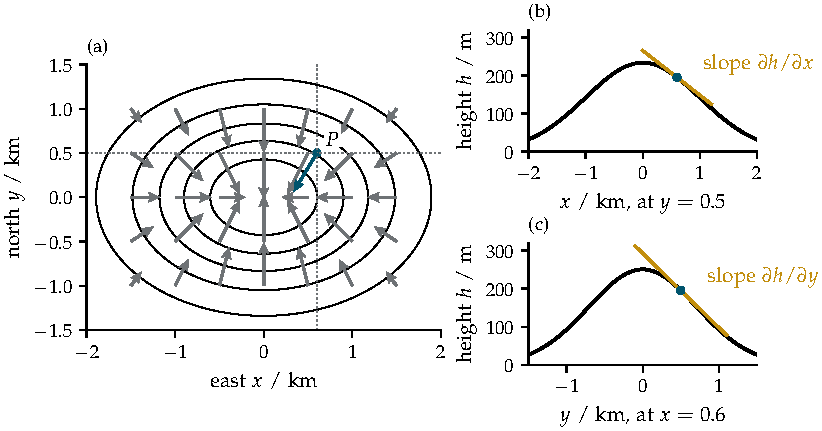
\includegraphics{ch03_energy/hill}
\caption{Partial derivatives and the gradient of a hill, $h =
300\,\mathrm{e}^{-(x^2 + 2y^2)/2}$\,\si{\metre}. (a) Contours every
\SI{50}{\metre}, with the gradient $\grad h$ at a grid of points (grey)
and at $P = (0.6, 0.5)$\,\si{\kilo\metre} (teal). Each arrow points
straight uphill, across the contours. (b) The height along the east-west
line through $P$ (dotted in a), whose slope at $P$ is $\partial h/\partial
x$. (c) The height along the north-south line through $P$, whose slope at
$P$ is $\partial h/\partial y$.}
\label{fig:en-hill}
\end{figure}

\begin{toolbox}[The gradient]
The two partial derivatives together give the change of height for a
short step in any direction. Step from $(x, y)$ to $(x + \Delta x, y +
\Delta y)$ in two legs, first east and then north, adding and subtracting
the height at the corner $(x + \Delta x, y)$:
\begin{align*}
   h(x + \Delta x, y + \Delta y) - h(x, y)
   &= \bigl[h(x + \Delta x, y + \Delta y) - h(x + \Delta x, y)\bigr]\\
   &\quad + \bigl[h(x + \Delta x, y) - h(x, y)\bigr] .
\end{align*}
The second bracket is a step east, and by the definition of $\partial
h/\partial x$ it is $(\partial h/\partial x)\,\Delta x$ plus an error
that is small compared with $\Delta x$. The first is a step north, taken
from the corner, so it is about $\Delta y$ times the northward slope at
the corner, with an error small compared with $\Delta y$; that slope
approaches the northward slope at $(x, y)$ as the step shrinks, provided that the slopes change smoothly from place to place, as
they do for this hill. Hence
\begin{equation*}
   \Delta h \approx \frac{\partial h}{\partial x}\,\Delta x
   + \frac{\partial h}{\partial y}\,\Delta y
   = \grad h\cdot\Delta\vb{r} ,
   \qquad
   \grad h = \Bigl(\frac{\partial h}{\partial x},
   \frac{\partial h}{\partial y}\Bigr) ,
\end{equation*}
with an error small compared with the length of the step $\Delta\vb{r} =
(\Delta x, \Delta y)$. The vector $\grad h$, read `grad $h$', is the
gradient of $h$; in three dimensions it has a third component, $\partial
h/\partial z$, and the step a third leg. Three consequences follow.
\begin{itemize}
\item \emph{Steepest ascent.} For a step of length $\ell$ in the
   direction of a unit vector $\vb{n}$, a vector of length 1, $\Delta\vb{r}
   = \ell\vb{n}$ and $\Delta h \approx \ell\,\grad h\cdot\vb{n}$. Dividing
   by $\ell$, the height changes at the rate $\grad h\cdot\vb{n} =
   \lvert\grad h\rvert\,\lvert\vb{n}\rvert\cos\theta = \lvert\grad
   h\rvert\cos\theta$ per unit distance, with $\theta$ the angle between
   $\vb{n}$ and $\grad h$. The rate is greatest for $\theta = 0$, where
   $\cos\theta = 1$: the gradient points up the steepest slope, and its
   length is that slope.
\item \emph{Contours.} Along a contour $h$ does not change, so for
   $\vb{n}$ pointing along the contour $\grad h\cdot\vb{n} = 0$: wherever
   $\grad h$ is not zero, it is perpendicular to the contour through the
   point.
\item \emph{Along a path.} If a point moves along a path $\vb{r}(t)$, then
   over a short interval $\Delta t$ it moves by $\Delta\vb{r} = \vb{r}(t +
   \Delta t) - \vb{r}(t)$ and the height changes by $\Delta h =
   h\bigl(\vb{r}(t + \Delta t)\bigr) - h\bigl(\vb{r}(t)\bigr)$, so
   \begin{align*}
      \frac{\Delta h}{\Delta t}
      &\approx \grad h\cdot\frac{\Delta\vb{r}}{\Delta t}
         && \text{dividing $\Delta h \approx \grad h\cdot\Delta\vb{r}$
            by $\Delta t$}\\
      \frac{\dd}{\dd t}\,h\bigl(\vb{r}(t)\bigr)
      &= \grad h\cdot\frac{\dd\vb{r}}{\dd t}
         && \text{letting $\Delta t \to 0$,}
   \end{align*}
   the chain rule along a path. The error of the first line is an error
   small compared with $\lvert\Delta\vb{r}\rvert$, divided by $\Delta t$;
   since $\lvert\Delta\vb{r}\rvert/\Delta t$ approaches $\lvert\dd\vb{r}/
   \dd t\rvert$, it vanishes in the limit.
\end{itemize}
At $P$ the gradient is $(-117.1, -195.2)$ metres per kilometre, of length
\begin{equation*}
   \lvert\grad h\rvert = \sqrt{117.1^2 + 195.2^2} = 227.6
\end{equation*}
metres per kilometre. That is a rise of $227.6/1000 = 0.2276$ metres per
metre, and the angle whose tangent is 0.2276 is \ang{12.8}. Walking
straight towards the summit instead, in the direction of the unit vector
$\vb{n} = (-0.6, -0.5)/0.781$, where $0.781 = \sqrt{0.6^2 + 0.5^2}$ is the
length of $(-0.6, -0.5)$, the height rises at the rate
\begin{equation*}
   \grad h\cdot\vb{n}
   = \frac{(-117.1)(-0.6) + (-195.2)(-0.5)}{0.781}
   = \frac{167.86}{0.781} = 214.9
\end{equation*}
metres per kilometre, less than 227.6: on elliptical contours the
steepest way up need not point at the summit (\cref{fig:en-hill}a); it
does only along the axes of the ellipses.
\end{toolbox}

\subsection*{The force is minus the gradient}

Now let $U(\vb{r})$ be the potential energy of a conservative force. For
a short straight step $\Delta\vb{r}$ from $\vb{r}$, the force hardly
changes along the step, so, since the work along the step is the drop
$U(A) - U(B)$ with $A = \vb{r}$ and $B = \vb{r} + \Delta\vb{r}$,
\cref{eq:en-work-constant} makes $U$ change by about $-\vb{F}\cdot\Delta
\vb{r}$. By the gradient toolbox it also changes by about $\grad U\cdot
\Delta\vb{r}$. The two agree, to within errors small compared with the
step, for steps in every direction, which is possible only if
\begin{equation}
   \vb{F} = -\grad U ,
   \qquad\text{that is,}\quad
   F_x = -\frac{\partial U}{\partial x},\quad
   F_y = -\frac{\partial U}{\partial y},\quad
   F_z = -\frac{\partial U}{\partial z} .
   \label{eq:en-gradient}
\end{equation}
Taking the step along $x$, for example, the first gives $-F_x\,\Delta x$
and the second $(\partial U/\partial x)\,\Delta x$; dividing both by
$\Delta x$ and letting the step shrink removes the errors, leaving $F_x =
-\partial U/\partial x$.

The converse holds as well. Suppose $\vb{F} = -\grad U$ for some $U$
with smoothly varying partial derivatives. Along any path $\vb{r}(s)$
from $A$ to $B$, the chain rule along a path gives $\vb{F}\cdot\dd\vb{r}/
\dd s = -\grad U\cdot\dd\vb{r}/\dd s = -\dd U(\vb{r}(s))/\dd s$, so the
line integral is
\begin{align*}
   \int_{s_A}^{s_B} -\frac{\dd}{\dd s}\,U\bigl(\vb{r}(s)\bigr)\,\dd s
   &= -\bigl[U(B) - U(A)\bigr]
      && \text{by the fundamental theorem of calculus}\\
   &= U(A) - U(B) ,
\end{align*}
the same for every path. \emph{A force is conservative exactly when it is
minus the gradient of a potential energy.} For the weight, $U = mgz$, and
$-\grad U = (0, 0, -mg)$, as it should be.

\Cref{eq:en-gradient} makes the force a property of the shape of $U$. By
the gradient toolbox, the force points in the direction in which the
potential energy falls fastest, its size is the steepest slope of $U$,
and it is perpendicular to the contours of $U$, which in space are
surfaces of equal $U$. A small block placed on the hillside of
\cref{fig:en-hill}(a), with no friction to hold it, is likewise pushed
straight down the slope, opposite to the arrows of $\grad h$. Where $\grad
U = \vb{0}$ the force vanishes, and a body at rest stays at rest. In two or
three dimensions most such equilibria are of three kinds: minima, from which every direction leads up; maxima, from
which every direction leads down; and saddle points, like a mountain
pass, which is the lowest point on the ridge between two valleys and the
highest point on the path through the pass. Chapter~4 develops the test
that tells them apart.

\begin{selfcheck}
On a map, the contours on one side of a hill are crowded together and on
the other side widely spaced. On which side is $\lvert\grad h\rvert$
larger? In which direction does $\grad h$ point where it crosses a
contour?
\end{selfcheck}

%=============================================================================!
% 3.11  THE CURL TEST                                                         !
%=============================================================================!
\section{The curl test}
\label{sec:en-curl}

Given a force, how can we tell whether it is conservative? Checking the
work along every path is impossible. This section derives a test that
uses only derivatives of the force at each point, and explains what the
test measures: how much the force circulates around a small loop.

\subsection*{A property of every gradient}

\begin{toolbox}[Mixed partial derivatives]
For a function $U(x, y)$ whose second partial derivatives change smoothly
from place to place, the order of differentiation does not matter,
\begin{equation*}
   \frac{\partial}{\partial x}\Bigl(\frac{\partial U}{\partial y}\Bigr)
   = \frac{\partial}{\partial y}\Bigl(\frac{\partial U}{\partial x}\Bigr) .
\end{equation*}
For $U = x^2y^3$, for instance, $\partial U/\partial y = 3x^2y^2$, whose
derivative with respect to $x$ is $6xy^2$, and $\partial U/\partial x =
2xy^3$, whose derivative with respect to $y$ is also $6xy^2$. To see why
it holds in general, take the combination of the values of $U$ at the four
corners of a small rectangle,
\begin{equation*}
   D = U(x + \Delta x, y + \Delta y) - U(x + \Delta x, y)
   - U(x, y + \Delta y) + U(x, y) ,
\end{equation*}
and group its four terms in two ways. Grouped as
\begin{equation*}
   D = \bigl[U(x + \Delta x, y + \Delta y) - U(x + \Delta x, y)\bigr]
   - \bigl[U(x, y + \Delta y) - U(x, y)\bigr] ,
\end{equation*}
each bracket is a step north, one taken at $x + \Delta x$ and one at $x$.
Holding $x$ fixed, the fundamental theorem of calculus makes each bracket
the integral of $\partial U/\partial y$ along its step, so, writing
$\frac{\partial U}{\partial y}(a, b)$ for its value at the point $(a, b)$,
\begin{equation*}
   D = \int_y^{y + \Delta y}\Bigl[\frac{\partial U}{\partial y}(x + \Delta
   x, y') - \frac{\partial U}{\partial y}(x, y')\Bigr]\dd y'
\end{equation*}
exactly. By the same theorem, now holding $y'$ fixed, the square bracket
is the integral of $\partial(\partial U/\partial y)/\partial x$ from $x$ to
$x + \Delta x$. Because this second derivative changes smoothly, on a
small enough rectangle it stays as close as we like to its value at $(x,
y)$, so $D$ is $\Delta x\,\Delta y$ times $\partial(\partial U/\partial
y)/\partial x$ at $(x, y)$, with an error small compared with $\Delta
x\,\Delta y$. Grouped instead as
\begin{equation*}
   D = \bigl[U(x + \Delta x, y + \Delta y) - U(x, y + \Delta y)\bigr]
   - \bigl[U(x + \Delta x, y) - U(x, y)\bigr] ,
\end{equation*}
each bracket is a step east, and the same argument with $x$ and $y$
exchanged makes $D$ equal to $\Delta x\,\Delta y$ times $\partial(\partial
U/\partial x)/\partial y$ at $(x, y)$, again with an error small compared
with $\Delta x\,\Delta y$. Both expressions describe the same number $D$,
so dividing by $\Delta x\,\Delta y$ and letting the rectangle shrink, the
two mixed derivatives are equal.
\end{toolbox}

If $\vb{F} = -\grad U$ in the plane, then $F_x = -\partial U/\partial x$
and $F_y = -\partial U/\partial y$, so by the toolbox
\begin{equation*}
   \frac{\partial F_y}{\partial x}
   = -\frac{\partial}{\partial x}\Bigl(\frac{\partial U}{\partial y}\Bigr)
   = -\frac{\partial}{\partial y}\Bigl(\frac{\partial U}{\partial x}\Bigr)
   = \frac{\partial F_x}{\partial y} .
\end{equation*}
Every conservative force whose components have smoothly changing partial
derivatives therefore has
\begin{equation}
   \frac{\partial F_y}{\partial x} - \frac{\partial F_x}{\partial y} = 0
   \label{eq:en-curl-zero}
\end{equation}
at every point. The swirl $c\,(-y, x)$ of \cref{eq:en-swirl} fails: $F_y
= cx$ gives $\partial F_y/\partial x = c$, $F_x = -cy$ gives $\partial
F_x/\partial y = -c$, and the difference is $2c$. The swirl is not
conservative, as its work around a circle already showed.

\subsection*{Circulation around a small loop}

The combination in \cref{eq:en-curl-zero} has a meaning of its own, which
the next box finds, and which turns the necessary condition into a test.

\begin{toolbox}[The curl]
Take the small rectangle of \cref{fig:en-loop}, with corners $(x, y)$ and
$(x + \Delta x, y + \Delta y)$, and add up the work of a force $\vb{F}$
once around it anticlockwise, taking the force at the middle of each
side.
\begin{itemize}
\item Along the bottom, eastwards, the displacement is $(\Delta x, 0)$:
   work $F_x\,\Delta x$, with $F_x$ taken at height $y$.
\item Up the right side: $F_y\,\Delta y$, with $F_y$ taken at $x +
   \Delta x$.
\item Along the top, westwards, the displacement is $(-\Delta x, 0)$:
   work $-F_x\,\Delta x$, with $F_x$ taken at height $y + \Delta y$.
\item Down the left side: $-F_y\,\Delta y$, with $F_y$ taken at $x$.
\end{itemize}
Pairing the two sides that run east and west, and the two that run north
and south, the total is
\begin{align*}
   \oint\vb{F}\cdot\dd\vb{r}
   &\approx \bigl[F_y(x + \Delta x) - F_y(x)\bigr]\,\Delta y
   - \bigl[F_x(y + \Delta y) - F_x(y)\bigr]\,\Delta x\\
   &\approx \frac{\partial F_y}{\partial x}\,\Delta x\,\Delta y
   - \frac{\partial F_x}{\partial y}\,\Delta y\,\Delta x
   = \Bigl(\frac{\partial F_y}{\partial x}
   - \frac{\partial F_x}{\partial y}\Bigr)\Delta A ,
\end{align*}
where each square bracket is the change of one component over one short
step, and $\Delta A = \Delta x\,\Delta y$ is the area. The combination in
brackets is therefore the work around a small loop per unit area
enclosed. The work around a closed loop is called its circulation, so the
combination is the circulation per unit area; it is called the curl of
$\vb{F}$ in the plane. In three dimensions a small loop can lie in the
$xy$, the $yz$ or the $zx$ plane. Renaming the letters in turn, $x$ to
$y$, $y$ to $z$ and $z$ to $x$, carries a loop in the $xy$ plane,
traversed anticlockwise as seen from the positive end of the $z$ axis,
into one in the $yz$ plane, anticlockwise as seen from the positive end of
the $x$ axis, and carries $\partial F_y/\partial x - \partial F_x/\partial
y$ into $\partial F_z/\partial y - \partial F_y/\partial z$; renaming once
more gives the $zx$ plane and $\partial F_x/\partial z - \partial
F_z/\partial x$. The three combinations form the curl vector, written
$\grad\times\vb{F}$ and read `curl $\vb{F}$' (the $\times$ is the cross
product of Chapter~5, not needed here),
\begin{equation*}
   \grad\times\vb{F} = \Bigl(
   \frac{\partial F_z}{\partial y} - \frac{\partial F_y}{\partial z},\;
   \frac{\partial F_x}{\partial z} - \frac{\partial F_z}{\partial x},\;
   \frac{\partial F_y}{\partial x} - \frac{\partial F_x}{\partial y}
   \Bigr) ,
\end{equation*}
whose third component is the one found above, for a loop in the $xy$
plane.

A large loop made of the sides of many small rectangles, tiling the
region it encloses, has a circulation equal to the sum of the
circulations of the small rectangles. Each inner side belongs to two
neighbouring rectangles and is traversed once in each direction, so its
two contributions cancel, and only the outer boundary is left. Hence the
work around the loop is the sum of the curl times $\Delta A$ over the
rectangles. As the rectangles shrink, such a sum of values times small
areas approaches a limit, written $\iint\dots\dd A$ and called the
integral over the area, just as a sum of values times short steps
approaches the integral of \cref{sec:mo-integrating}; when the value is a
constant, the sum, and so the integral, is that constant times the whole
area. So
\begin{equation*}
   \oint\vb{F}\cdot\dd\vb{r} = \iint\Bigl(\frac{\partial F_y}{\partial x}
   - \frac{\partial F_x}{\partial y}\Bigr)\dd A ,
\end{equation*}
a result known as Green's theorem, for a loop traversed anticlockwise. It
needs $\vb{F}$ and its partial derivatives to change smoothly at every
point inside the loop, because every small rectangle of the tiling must
have a curl. A smooth curved loop is approached by staircases of ever
smaller rectangles. A staircase never becomes as short as the curve, which
would matter for friction; but for a force that depends only on position,
the work over each short stretch is nearly $\vb{F}\cdot\Delta\vb{r}$, and
the staircase and the stretch of curve beside it share the same
displacement $\Delta\vb{r}$, so the theorem holds for the curve too.
\end{toolbox}

\begin{figure}[htb]
\centering
\begin{tikzpicture}[line cap=round, line join=round, scale=1.1,
   side/.style={-{Stealth[length=5pt]}, line width=0.9pt, accent}]
   \draw[side] (0,0) -- (3,0) node[midway, below] {\small $F_x\,\Delta x$
      at $y$};
   \draw[side] (3,0) -- (3,2) node[midway, right] {\small $F_y\,\Delta y$
      at $x + \Delta x$};
   \draw[side] (3,2) -- (0,2) node[midway, above] {\small $-F_x\,\Delta x$
      at $y + \Delta y$};
   \draw[side] (0,2) -- (0,0) node[midway, left] {\small $-F_y\,\Delta y$
      at $x$};
   \fill (0,0) circle (1.3pt) node[below left] {\small $(x, y)$};
   \fill (3,2) circle (1.3pt) node[above right]
      {\small $(x + \Delta x, y + \Delta y)$};
\end{tikzpicture}
\caption{The work of a force once anticlockwise around a small rectangle,
side by side. The two sides that run east and west differ only in their
height, and the two that run north and south only in their east-west
position.}
\label{fig:en-loop}
\end{figure}

\subsection*{The test}

The curl test now reads in both directions. If a force is conservative,
its curl is zero everywhere, by \cref{eq:en-curl-zero}. Conversely, if
the curl is zero everywhere in a region with no holes, every loop in the
region encloses only points of the region, so Green's theorem makes the
work around it zero; within the region the work then does not depend on
the path, and the force is conservative there. In three dimensions
the same holds, because any loop can be spanned by a surface tiled with
small loops in the same way, a result called Stokes' theorem whose details
we do not need. The proviso about holes is real: \cref{ex:en-vortex} gives
a force whose curl is zero wherever it is defined, but which is not
defined at the origin, and whose work around the origin is not zero.

For the swirl, with curl $2c$ everywhere, Green's theorem gives the work
anticlockwise around any loop as $2c$ times the area it encloses. On the
circle of the line-integral toolbox that is $2c\times\pi R^2 = 2\pi
cR^2$, as computed there directly.

When the test is passed, $U$ follows from \cref{eq:en-potential-3d} along
whichever path is easiest. From the origin, go along the $x$ axis to $(x,
0)$, a leg on which only $F_x$ does work, and then straight north to $(x,
y)$, on which only $F_y$ does:
\begin{equation*}
   U(x, y) = -\int_0^x F_x(x', 0)\,\dd x' - \int_0^y F_y(x, y')\,\dd y' .
\end{equation*}

For many atoms the test has the same form, with every pair of the $3N$
coordinates in place of $x$ and $y$. Numbering the coordinates $q_1,
\dots, q_{3N}$, a force is conservative only if
\begin{equation*}
   \frac{\partial F_a}{\partial q_b} = \frac{\partial F_b}{\partial q_a}
   \qquad\text{for every pair $a$ and $b$,}
\end{equation*}
where $F_a$ is the force component along $q_a$. For a conservative
force these derivatives are minus the second derivatives of $U$, which
Chapter~4 collects into a table called the Hessian.

\notebook{03}{compute the curl of a force symbolically, and the work
around loops}

\begin{selfcheck}
Is the force $\vb{F} = (y, x)$ conservative? If so, find a potential
energy $U$ with $\vb{F} = -\grad U$.
\end{selfcheck}

%=============================================================================!
% 3.12  THE ENERGY OF ATOMS                                                   !
%=============================================================================!
\section{The energy of atoms}
\label{sec:en-atoms}

Every result of this chapter was found with boxes, beads and carts. This
section carries them to atoms: it introduces the unit in which the
energies of atoms are measured, converts the kinetic energy into the
units of this book, and proves that Newton's laws conserve the total
energy of any number of atoms whose forces come from a potential energy.

\subsection*{The electronvolt}

The joule is far too large a unit for a single atom. The lithium atom of
\cref{sec:ne-atoms}, of mass $6.94\times\SI{1.66054e-27}{\kilogram} =
\SI{1.1524e-26}{\kilogram}$, moving at \SI{1390}{\metre\per\second} after
\SI{10}{\femto\second} under a force of \SI{1}{\electronvolt\per
\angstrom}, has a kinetic energy of $\frac12\times1.1524\times10^{-26}
\times1390^2 = \SI{1.113e-20}{\joule}$. Energies of atoms are therefore
measured in electronvolts, the unit already used for forces in
\cref{sec:ne-atoms}, with
\begin{equation*}
   \SI{1}{\electronvolt} = \SI{1.602176634e-19}{\joule}
\end{equation*}
exactly. The name comes from electricity, which this book does not need;
the size of the unit in joules is fixed by the definition of the SI units,
and only its size matters here. The lithium atom has $1.113\times10^{-20}/1.602\times
10^{-19} = \SI{0.0695}{\electronvolt}$, and \cref{sec:ne-atoms} found
that it had moved \SI{0.0695}{\angstrom}. The force of
\SI{1}{\electronvolt\per\angstrom} has done
$1\times0.0695 = \SI{0.0695}{\electronvolt}$ of work on it, equal to its
kinetic energy, as the work-energy theorem requires.

\subsection*{Kinetic energy in eV, \AA, fs and amu}

With masses in atomic mass units and velocities in
\si{\angstrom\per\femto\second}, the product $\frac12 mv^2$ comes out in
\si{\amu\angstrom\squared\per\femto\second\squared}, which is not the
electronvolt; Newton's law needed a conversion factor in
\cref{sec:ne-atoms} for the same reason. We convert one unit of each
kind. A mass of \SI{1}{\amu} is \SI{1.66053906892e-27}{\kilogram}, and a
velocity of \SI{1}{\angstrom\per\femto\second} is $10^{-10}/10^{-15} =
\SI{e5}{\metre\per\second}$, whose square is
\SI{e10}{\metre\squared\per\second\squared}. Their product is, in joules,
\begin{equation*}
   \SI{1}{\amu\angstrom\squared\per\femto\second\squared}
   = 1.66053906892\times10^{-27}\times10^{10}\,\si{\joule}
   = \SI{1.66053906892e-17}{\joule} ,
\end{equation*}
since $-27 + 10 = -17$. Dividing by the size of an electronvolt in joules,
\begin{equation*}
   \frac{1.66053906892\times10^{-17}}{1.602176634\times10^{-19}}
   = 1.036427\times10^{2} = 103.6427 ,
\end{equation*}
where $1.66053906892/1.602176634 = 1.036427$ and $10^{-17}/10^{-19} =
10^{-17-(-19)} = 10^{2}$. Therefore
\begin{equation}
   \SI{1}{\amu\angstrom\squared\per\femto\second\squared}
   = \SI{103.6427}{\electronvolt} ,
   \qquad
   K\,[\si{\electronvolt}] = \tfrac12\,m\,[\si{\amu}]\;
   v^2\,[\si{\angstrom\squared\per\femto\second\squared}]
   \times103.6427 .
   \label{eq:en-mv2}
\end{equation}
This factor and the factor of Newton's law, \num{9.648533e-3}, are each
other's inverse, $1/103.6427 = \num{9.648533e-3}$, and for a reason.
\Cref{eq:en-mv2} says that one electronvolt is $1/103.6427$ of an
\si{\amu\angstrom\squared\per\femto\second\squared}, so a force of
\SI{1}{\electronvolt\per\angstrom}, divided by a mass of \SI{1}{\amu},
is $(1/103.6427)\,\si{\amu\angstrom\squared\per\femto\second\squared}$
divided by \si{\angstrom\amu}, which, cancelling the \si{\amu} and one
\si{\angstrom}, is $(1/103.6427)\,\si{\angstrom\per\femto\second\squared}$:
both factors
express the electronvolt in atomic mass units, \aa ngstr\"oms and
femtoseconds. In \texttt{mdlab} the kinetic-energy factor is
\texttt{MV2\_TO\_EV}, computed from the CODATA values of the constants,
and the Newton factor \texttt{FORCE\_TO\_ACCEL} is defined as its inverse,
so the two can never disagree. The kinetic energy of a group of atoms is
then a few lines.

\begin{code}
def kinetic_energy(masses: ArrayLike, velocities: ArrayLike) -> float:
    masses = np.asarray(masses, dtype=float)
    velocities = np.asarray(velocities, dtype=float)
    speed_squared = np.sum(velocities**2, axis=-1)  # v · v, one per atom
    if masses.ndim > 0 and masses.shape != speed_squared.shape:
        raise ValueError("give one mass for each row of velocities")
    in_amu_a2_per_fs2 = 0.5 * np.sum(masses * speed_squared)
    return float(in_amu_a2_per_fs2) * units.MV2_TO_EV
\end{code}

The velocities arrive with one row per atom and one column per component,
as the forces did in \cref{sec:ne-atoms}. Squaring the array squares every
component, and adding along the last axis, \texttt{axis=-1}, adds the
three squared components within each row, which is $\vb{v}_i\cdot
\vb{v}_i$ for each atom $i$. The check applies when the masses come as a
list, for which \texttt{masses.ndim}, the number of dimensions of the
array, is 1: it stops the function with a message unless
\texttt{masses.shape}, the length of each dimension, matches that of the
squared speeds, one mass for each atom. A single number, which has no
dimensions, skips the check and serves as the mass of every atom. Multiplying the masses by the squared
speeds pairs each atom's mass with its own speed, the sum over atoms and
the factor one half give $\sum_i\frac12 m_i v_i^2$ in
\si{\amu\angstrom\squared\per\femto\second\squared}, and the last line
converts to electronvolts. The lithium atom, which moves along a line
and so has a velocity of one component, called as
\texttt{kinetic\_energy(6.94, [0.0139])}, returns
\SI{0.0695}{\electronvolt}.

\subsection*{The potential energy of many atoms}

For $N$ atoms the potential energy is a function of all their positions,
$U(\vb{r}^N)$, a function of $3N$ coordinates. Chapter~8 shows where such
functions come from; here we need only that the force on each atom is
minus the gradient of $U$ with respect to that atom's own coordinates,
\begin{equation}
   \vb{F}_i = -\grad_i U
   = -\Bigl(\frac{\partial U}{\partial x_i}, \frac{\partial U}{\partial
   y_i}, \frac{\partial U}{\partial z_i}\Bigr) ,
   \label{eq:en-force-atoms}
\end{equation}
where the subscript on $\grad_i$ says which atom's coordinates are
differentiated, all the others held fixed. Everything in
\cref{sec:en-paths,sec:en-gradient,sec:en-curl} carries over with $3N$
coordinates in place of three: a path moves all the atoms at once, from
one arrangement to another; the work done on them along it is the sum
over atoms of $\vb{F}_i\cdot\Delta\vb{r}_i$ added over its short steps,
and for these forces it is the drop in $U$ between the two
arrangements.

\begin{proposition}
\label{prop:en-energy-atoms}
Let $N$ atoms move according to Newton's second law, $m_i\,\dd\vb{v}_i/\dd
t = \vb{F}_i$, with forces $\vb{F}_i = -\grad_i U(\vb{r}^N)$ from a
potential energy that does not depend on time except through the
positions. Then the total energy
\begin{equation*}
   E = \sum_{i=1}^{N}\tfrac12 m_i v_i^2 + U(\vb{r}^N)
\end{equation*}
is constant along every motion.
\end{proposition}

\begin{proof}
By \cref{sec:en-varying}, applied to each atom, the kinetic energy changes
at the rate $\dd K/\dd t = \sum_i\vb{F}_i\cdot\vb{v}_i$, where $K =
\sum_i\frac12 m_i v_i^2$, the sum of the
powers of the forces; this is where the second law enters. The gradient
toolbox of \cref{sec:en-gradient}, with a step of $3N$ legs, one along
each coordinate, in place of two, gives, grouping the legs atom by atom,
\begin{equation*}
   \Delta U \approx \sum_{i=1}^{N}\Bigl(\frac{\partial U}{\partial x_i}
   \Delta x_i + \frac{\partial U}{\partial y_i}\Delta y_i
   + \frac{\partial U}{\partial z_i}\Delta z_i\Bigr)
   = \sum_{i=1}^{N}\grad_i U\cdot\Delta\vb{r}_i ,
\end{equation*}
and the chain rule along a path then reads
\begin{equation*}
   \frac{\dd U}{\dd t} = \sum_{i=1}^{N}\grad_i U\cdot\frac{\dd\vb{r}_i}{\dd
   t} = -\sum_{i=1}^{N}\vb{F}_i\cdot\vb{v}_i .
\end{equation*}
The two rates cancel, so $\dd E/\dd t = 0$.
\end{proof}

A potential energy that depends only on the distance between two atoms,
like the energy $\frac12 k\xi^2$ of the spring between the carts of
\cref{sec:en-bodies}, is of this form, and \cref{ex:en-pair} shows that
for it \cref{eq:en-force-atoms}
produces the equal and opposite forces of the third law by itself.

\Needspace{10\baselineskip}
\begin{bridge}
In Born--Oppenheimer molecular dynamics, $U(\vb{r}^N)$ is the
ground-state energy of the electrons with the nuclei held at $\vb{r}^N$,
plus the repulsion between the nuclei, and the forces are its negative
gradient. The Hellmann--Feynman theorem supplies the part that comes from
the explicit dependence of the Hamiltonian on the nuclear positions, and
the Pulay terms add the part that comes from basis functions moving with
the atoms. A force computed without the Pulay terms, or from an
incompletely converged density, is not exactly $-\grad_i U$ of the energy
reported with it, and \cref{sec:en-drift} shows what such a discrepancy
does to the total energy.
\end{bridge}

\begin{selfcheck}
An oxygen atom (\SI{15.999}{\amu}) moves at
\SI{0.01}{\angstrom\per\femto\second}. What is its kinetic energy in
electronvolts?
\end{selfcheck}

%=============================================================================!
% 3.13  A LITHIUM ATOM ON A MODEL SURFACE                                     !
%=============================================================================!
\section{A lithium atom on a model surface}
\label{sec:en-surface}

The bead on its wire showed what an energy diagram says in one dimension.
This section draws the same picture for an atom moving in two: a lithium
atom on a layer of carbon atoms arranged in hexagons, as in a sheet of
graphite. We build a simple model of its potential energy, check that
its force does the same work along every path, and follow the atom as it
hops from site to site with its total energy fixed.

\subsection*{The model}

A lithium atom resting on a carbon layer feels a potential energy that
depends on where it sits relative to the carbon atoms. We follow only its
motion parallel to the layer, at a fixed height, with the carbon atoms
held still, so $U$ is a function of the two coordinates $\vb{r} = (x,
y)$. Our model has three kinds of site (\cref{fig:en-surface}a). Above
the centre of a hexagon, a hollow, we make the energy lowest. Above a
carbon atom, a top, we make it highest. Midway between two neighbouring hollows, above the middle
of the bond shared by their hexagons, lies a bridge, the lowest point of
the ridge between the two hollows, and so a saddle point
(\cref{sec:en-gradient}). We take the spacing of neighbouring hollows to
be $a = \SI{2.46}{\angstrom}$, chosen to resemble the hexagons of a layer
of graphite, and the rise from a hollow to a bridge, the barrier, to be $U_{\mathrm b} =
\SI{0.3}{\electronvolt}$. Both are chosen to make the model easy to read;
neither is fitted to any measurement or calculation.

A simple function with this pattern is a sum of three ripples. A single
ripple $\cos(\vb{g}\cdot\vb{r})$, for a fixed vector $\vb{g}$, is
constant along every line perpendicular to $\vb{g}$, since moving along
such a line leaves $\vb{g}\cdot\vb{r}$ unchanged, and it rises and falls
like a sheet of corrugated iron as $\vb{r}$ moves along $\vb{g}$, with
crests $2\pi/\lvert\vb{g}\rvert$ apart. Three such ripples whose vectors
$\vb{g}_1$, $\vb{g}_2$ and $\vb{g}_3$ point at \ang{-30}, \ang{90} and
\ang{210}, all of length $\lvert\vb{g}\rvert = 4\pi/(\sqrt3\,a) =
\SI{2.949}{\per\angstrom}$, so that their crests lie $2\pi/\lvert\vb{g}
\rvert = \sqrt3\,a/2 = \SI{2.130}{\angstrom}$ apart, the distance $a\sin
\ang{60}$ between neighbouring rows of hollows, cross to make a hollow
above the centre of every hexagon, and we set
\begin{equation}
   U(\vb{r}) = \frac{U_{\mathrm b}}{4}\,\Bigl[\,3 - \cos(\vb{g}_1\cdot\vb{r})
   - \cos(\vb{g}_2\cdot\vb{r}) - \cos(\vb{g}_3\cdot\vb{r})\Bigr] .
   \label{eq:en-surface}
\end{equation}
At the origin all three cosines are 1, and $U = 0$: the origin is a
hollow. At the bridge $(a/2, 0)$, using $\vb{g}_k\cdot\vb{r} =
\lvert\vb{g}\rvert\lvert\vb{r}\rvert\cos\theta_k$ with $\theta_k$ the
angle between them (\cref{sec:mo-plane}), and $\lvert\vb{g}\rvert\,a/2 =
2\pi/\sqrt3$,
\begin{align*}
   \vb{g}_1\cdot\vb{r} &= \tfrac{2\pi}{\sqrt3}\cos\ang{-30} = \pi , &
   \vb{g}_2\cdot\vb{r} &= \tfrac{2\pi}{\sqrt3}\cos\ang{90} = 0 , &
   \vb{g}_3\cdot\vb{r} &= \tfrac{2\pi}{\sqrt3}\cos\ang{210} = -\pi ,
\end{align*}
since $\cos\ang{-30} = \sqrt3/2$ and $\cos\ang{210} = -\sqrt3/2$. The
cosines are $-1$, $1$ and $-1$, and $U = (U_{\mathrm b}/4)\bigl(3 - (-1) - 1 -
(-1)\bigr) = (U_{\mathrm b}/4)\times4 = U_{\mathrm b}$. The top $(a/2, a/(2\sqrt3))$
lies a distance $\sqrt{a^2/4 + a^2/12} = \sqrt{a^2/3} = a/\sqrt3 =
\SI{1.420}{\angstrom}$ from the hollow, in the direction at \ang{30} to the
$x$ axis, since $\tan\theta = \bigl(a/(2\sqrt3)\bigr)/(a/2) = 1/\sqrt3$.
There $\lvert\vb{g}\rvert\,a/\sqrt3 = 4\pi/3$, and the angles from
$\vb{r}$ to $\vb{g}_1$, $\vb{g}_2$ and $\vb{g}_3$ are \ang{60}, \ang{60}
and \ang{180}, so the three products are $\frac{4\pi}{3}\cos\ang{60} =
2\pi/3$, $2\pi/3$ and $\frac{4\pi}{3}\cos\ang{180} = -4\pi/3$. Each cosine
is $-\frac12$ (\cref{ex:en-top} checks this in components), and $U = (U_{\mathrm b}/4)(3 + \frac32) = 9U_{\mathrm b}/8 =
\SI{0.3375}{\electronvolt}$. Shifting $\vb{r}$ by $a$ along $x$ changes
$\vb{g}_1\cdot\vb{r}$ by $2\pi$, $\vb{g}_2\cdot\vb{r}$ by 0 and
$\vb{g}_3\cdot\vb{r}$ by $-2\pi$, which leaves every cosine unchanged, and
the same holds for a shift by $a$ at \ang{60}, so the pattern repeats from
hollow to hollow.

The force follows from \cref{eq:en-gradient}. Writing $\vb{g}\cdot\vb{r} =
g_x x + g_y y$, the chain rule gives $\partial\cos(\vb{g}\cdot\vb{r})/
\partial x = -g_x\sin(\vb{g}\cdot\vb{r})$, and likewise with $g_y$ for
$y$, so $\grad\cos(\vb{g}\cdot\vb{r}) = -\sin(\vb{g}\cdot\vb{r})\,\vb{g}$,
and
\begin{align*}
   \grad U &= \frac{U_{\mathrm b}}{4}\sum_{k=1}^{3}\sin(\vb{g}_k\cdot\vb{r})\,
      \vb{g}_k
      && \text{the 3 is constant, and each $-\cos$ gives $+\sin$,}\\
   \vb{F} = -\grad U &= -\frac{U_{\mathrm b}}{4}\sum_{k=1}^{3}
      \sin(\vb{g}_k\cdot\vb{r})\,\vb{g}_k .
\end{align*}
At the hollow and the bridge every sine is zero, since $\sin 0 =
\sin(\pm\pi) = 0$. At the top the three sines are equal, because
$\sin(-4\pi/3) = \sin(-4\pi/3 + 2\pi) = \sin(2\pi/3)$, so the force is
proportional to $\vb{g}_1 + \vb{g}_2 + \vb{g}_3$, which is zero: the $x$
components of the three directions add to $\cos\ang{-30} + \cos\ang{90} +
\cos\ang{210} = \sqrt3/2 + 0 - \sqrt3/2 = 0$, and the $y$ components to
$-\frac12 + 1 - \frac12 = 0$. Every site is an equilibrium. The function \texttt{energy.hexagonal\_surface} of
\texttt{mdlab} returns $U$ and $\vb{F}$ together, and its tests check the
force against central differences of $U$ and the site energies above.

\subsection*{Work on the surface}

\Cref{fig:en-surface}(a) shows the contours of $U$, the force, and two
paths from the hollow $A$ at the origin to the top $B$ at $(3.69,
0.710)$\,\si{\angstrom}, one spacing $a$ along $x$ from the top nearest
$A$: a straight line, and an arc that bulges to its left, lying
$1.2\sin(\pi s)$\,\si{\angstrom} from the line at the point a fraction $s$
of the way along it, so \SI{1.2}{\angstrom} at the middle. The function \texttt{work} gives
\SI{-0.3375}{\electronvolt} along both, equal to $U(A) - U(B)$, as a
conservative force requires. In \cref{fig:en-surface}(b) the swirl of
\cref{eq:en-swirl}, centred on $A$ with $c = \SI{0.005}{\electronvolt
\per\angstrom\squared}$, is added to the force. Along the straight path,
which runs directly away from the centre of the swirl, the swirl is
perpendicular to the path and does no work, so the work stays at
\SI{-0.3375}{\electronvolt}. Along the arc it is
\SI{-0.3662}{\electronvolt}. The arc followed by the straight path
backwards is a clockwise loop, and the curl of the total force is $0 +
2c$, the surface force being a gradient, so by Green's theorem the work
round this loop, $W_{\mathrm{arc}} - W_{\mathrm{straight}}$, is $-2c$
times the area between the paths. That area is the bulge integrated along
the chord, of length $\lvert AB\rvert = \sqrt{3.69^2 + 0.710^2} =
\SI{3.758}{\angstrom}$, on which a step $\dd s$ in the fraction moves
$\lvert AB\rvert\,\dd s$,
$\int_0^1 1.2\sin(\pi s)\,\lvert AB\rvert\,\dd s = 2\times1.2\times
3.758/\pi = \SI{2.871}{\angstrom\squared}$, using $\int_0^1\sin(\pi s)\,
\dd s = [-\cos(\pi s)/\pi]_0^1 = 2/\pi$; and $2c\times2.871 =
\SI{0.0287}{\electronvolt}$ is exactly the difference between the two
works.

\begin{figure}[htb]
\centering
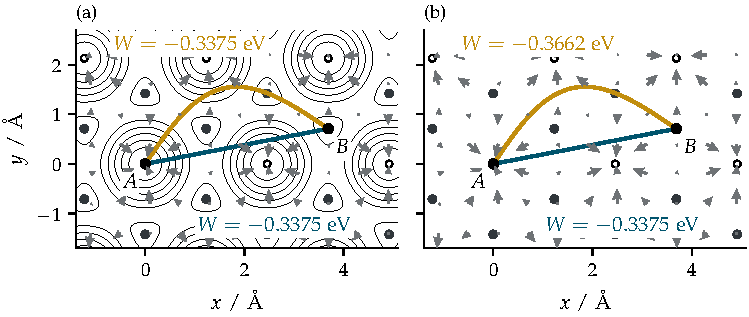
\includegraphics{ch03_energy/surface}
\caption{Work on the model surface. Open circles mark hollows and dark
dots the carbon atoms, at the tops. (a) Contours of $U$ at 0.05, 0.10,
0.15, 0.20, 0.25 and \SI{0.32}{\electronvolt}, the force $-\grad U$
(grey arrows), and two paths from the hollow $A$ to the top $B$; the work
is \SI{-0.3375}{\electronvolt} along both. (b) The same paths after a
swirl with $c = \SI{0.005}{\electronvolt\per\angstrom\squared}$, centred
on $A$, is added to the force (grey arrows). No potential energy exists to
contour, and the works differ by \SI{0.0287}{\electronvolt}.}
\label{fig:en-surface}
\end{figure}

\subsection*{Hopping with a fixed energy}

A lithium atom leaves the hollow at the origin with \SI{0.33}{
\electronvolt} of kinetic energy, \SI{10}{\percent} more than the barrier
$U_{\mathrm b}$, moving at \ang{37.5} to the $x$ axis. By \cref{eq:en-mv2} its
speed is
\begin{equation*}
   v = \sqrt{\frac{2K}{m\times103.6427}}
   = \sqrt{\frac{2\times0.33}{6.94\times103.6427}}
   = \SI{0.03029}{\angstrom\per\femto\second} ,
\end{equation*}
about \SI{3000}{\metre\per\second}. Its total energy, $E =
\SI{0.33}{\electronvolt}$, exceeds $U$ everywhere except in small islands
around each carbon atom, where $U$ rises to \SI{0.3375}{\electronvolt}:
the atom may go anywhere on the surface except into these islands, just
as the bead at $h_E = \SI{1.3}{\metre}$ could go anywhere except up the ends
of its track. \Cref{fig:en-li} shows the motion over
\SI{1.5}{\pico\second}, or \SI{1500}{\femto\second} (a picosecond is
\SI{1000}{\femto\second}), computed by a computer solution of the equations
of motion, a method from SciPy, a library of scientific routines for Python, that
advances the state in
short steps, as in \cref{sec:ne-equations}, but combines several force
evaluations per step and adjusts each step so that the error it
estimates for that step stays below about one part in $10^{11}$; over
many steps these small errors add up. Chapter~9 develops the methods that
molecular dynamics itself uses. The atom crosses from hollow to hollow
four times, visiting five hollows, while its kinetic energy rises and falls between
\num{0.0005} and \SI{0.33}{\electronvolt}. Its total energy stays at
\SI{0.33}{\electronvolt} to within \SI{2.5e-11}{\electronvolt}, which is
the error of the computer solution.

\begin{figure}[htb]
\centering
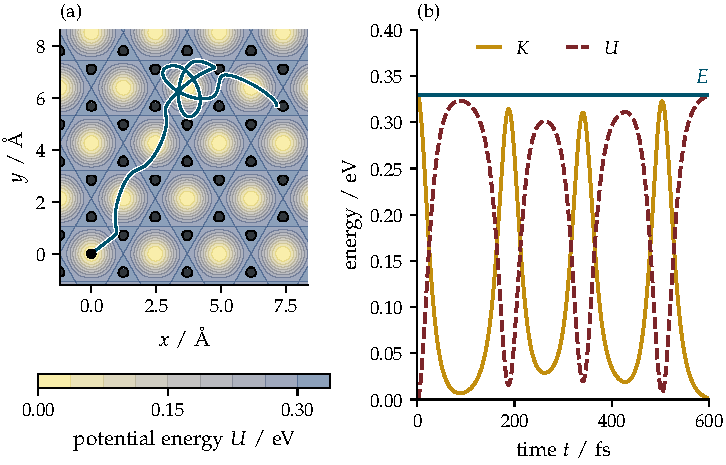
\includegraphics{ch03_energy/li_energy}
\caption{A lithium atom of \SI{6.94}{\amu} on the model surface, leaving
the hollow at the origin with \SI{0.33}{\electronvolt} of kinetic energy.
(a) The potential energy, shaded from the hollows (light) to the bridges
and tops (dark), the boundary $U = E$ of the islands around the carbon
atoms (dots), where the atom may not go, and its path over
\SI{1.5}{\pico\second}. (b) Kinetic, potential and total energy over the
first \SI{600}{\femto\second}.}
\label{fig:en-li}
\end{figure}

With less energy the picture changes as it did on the track. Below the
barrier, $E < \SI{0.3}{\electronvolt}$, the allowed region breaks into
separate patches, one around each hollow, and an atom stays in the hollow
it starts in, rattling about its bottom. To hop to a neighbouring hollow
it needs at least the barrier as kinetic energy at the bottom of the
hollow, a speed there of at least $\sqrt{2\times0.3/(6.94\times103.6427)}
= \SI{0.02888}{\angstrom\per\femto\second}$. Real atoms exchange energy
with their neighbours all the time, and Chapter~12 gives the odds that one
collects as much as the barrier; Chapters~16 and 17 measure how fast lithium spreads through graphite by
such hops.

\notebook{03}{launch the lithium atom with your own energy and direction}

\begin{selfcheck}
A lithium atom at the bottom of a hollow of the model surface has
\SI{0.25}{\electronvolt} of kinetic energy. Can it reach a neighbouring
hollow? How fast is it moving where $U = \SI{0.1}{\electronvolt}$?
\end{selfcheck}

%=============================================================================!
% 3.14  WHEN THE ENERGY CHANGES                                               !
%=============================================================================!
\section{When the energy changes}
\label{sec:en-drift}

\Cref{prop:en-energy-atoms} needs two conditions: every force is minus the
gradient of a potential energy, and that potential energy does not change
with time on its own. This section works out what happens to the total
energy of a group of atoms when either fails, and why that makes the
energy the first thing to check in a simulation of atoms isolated from
their surroundings.

\subsection*{A force that is not a gradient}

Write the force on each atom as a conservative part plus the rest,
$\vb{F}_i = -\grad_i U + \vb{F}_i^{\mathrm{nc}}$. The rest adds to the
power that changes the kinetic energy, $\dd K/\dd t = \sum_i\vb{F}_i
\cdot\vb{v}_i$, but not to the rate of change of $U$, which the chain rule
along a path still gives as $\sum_i\grad_i U\cdot\vb{v}_i$. Adding the two
rates,
\begin{align}
   \frac{\dd E}{\dd t}
   &= \sum_{i=1}^{N}\bigl(-\grad_i U + \vb{F}_i^{\mathrm{nc}}\bigr)\cdot
      \vb{v}_i + \sum_{i=1}^{N}\grad_i U\cdot\vb{v}_i \nonumber\\
   &= \sum_{i=1}^{N}\vb{F}_i^{\mathrm{nc}}\cdot\vb{v}_i ,
      \qquad\text{the gradient terms cancelling,}
   \label{eq:en-dEdt}
\end{align}
the rate at which the non-conservative forces do work, as for the box on
the floor in \cref{eq:en-dEdt-1d}. A drag on every atom, $\vb{F}_i^{
\mathrm{nc}} = -\gamma m_i\vb{v}_i$ with the drag rate $\gamma$ of
\cref{sec:ne-drag}, gives, since $\vb{v}_i\cdot\vb{v}_i = v_i^2$ and
$\sum_i m_i v_i^2 = 2K$,
\begin{equation*}
   \frac{\dd E}{\dd t} = -\gamma\sum_{i=1}^{N} m_i v_i^2 = -2\gamma K ,
\end{equation*}
so the energy can only fall. Chapter~13 adds such a drag on purpose, with
random kicks that make up for it, to hold atoms at a chosen temperature.

The swirl shows what a force does that sometimes adds energy and
sometimes removes it.
\Cref{fig:en-drift} repeats the motion of \cref{fig:en-li} with the swirl
of \cref{fig:en-surface}(b) added to the force. The total energy now
wanders, from \SI{0.0185}{\electronvolt} below its starting value to
\SI{0.0117}{\electronvolt} above it within \SI{1.5}{\pico\second}. The
power of the swirl is $\vb{F}_{\mathrm{sw}}\cdot\vb{v} = c\,(x v_y - y
v_x)$, so the atom gains energy while it moves anticlockwise about the
origin and loses it while it moves clockwise: on the positive $x$ axis, for
instance, $y = 0$ and the power is $c\,x v_y$, positive when the atom
moves up, which is anticlockwise there. Its change agrees with the work done by the swirl, the integral
of \cref{eq:en-dEdt} over time, to within \SI{1e-8}{\electronvolt}.

\begin{figure}[htb]
\centering
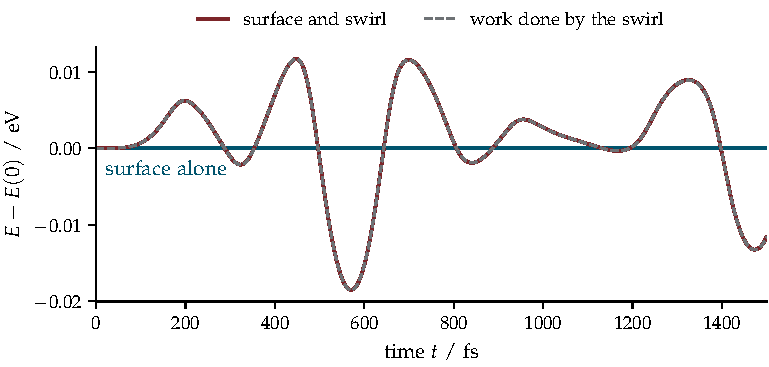
\includegraphics{ch03_energy/drift}
\caption{The lithium atom of \cref{fig:en-li}, launched in the same way on
the surface alone (teal) and with the swirl of \cref{fig:en-surface}(b)
added to the force (dark red). The change of the total energy $E = K + U$
from its starting value is shown against time, with the work done by the
swirl, $\int_0^t\vb{F}_{\mathrm{sw}}\cdot\vb{v}\,\dd t'$ (dashed), which it follows to within \SI{1e-8}{\electronvolt}.}
\label{fig:en-drift}
\end{figure}

\subsection*{A potential energy that changes with time}

If the potential energy also depends on time, $U(\vb{r}^N, t)$, because
something outside the atoms is being changed while they move, then $U$
changes even when the atoms stand still. A step in time, $\Delta t$, is
then one more leg of the gradient toolbox's step, and the chain rule along
a path gains one term, the partial derivative with respect to time,
\begin{equation*}
   \frac{\dd U}{\dd t} = \sum_{i=1}^{N}\grad_i U\cdot\vb{v}_i
   + \frac{\partial U}{\partial t} ,
\end{equation*}
so that, with conservative forces, $\dd E/\dd t = \partial U/\partial t$.
A hand that moves the far end of a spring does work on the body at the
near end in this way: with the hand at $X(t)$, measured so that the spring
is slack when the body is at $x = X$, the body has the potential energy $U
= \frac12 k\,(x - X(t))^2$, which changes even while the body stands
still. So does a wall pushed in to squeeze a group of atoms, the picture
behind the pistons with which Chapter~14 controls their pressure.

\Needspace{12\baselineskip}
\begin{practice}
The exact motion of an isolated group of atoms, one that exchanges no
energy with its surroundings, keeps $E$ constant. A simulation of such a
group whose total energy drifts is therefore not following the exact
motion, and there are two common causes. The first is the finite time
step with which the equations of motion are advanced, the subject of
Chapter~9. The second is a force that is not exactly $-\grad_i U$ of the
potential energy reported with it, for which \cref{eq:en-dEdt} gives the
drift directly: an error in the code that computes the forces, a
potential energy cut off abruptly at some distance (Chapter~8), or a machine-learned
model, a program fitted to examples of computed forces (Part~V), that
predicts the forces directly instead of differentiating an
energy, so that nothing constrains their curl. Bigi, Langer and Ceriotti
found that models of the last kind can make several types of molecular
dynamics unstable and the convergence of geometry optimisation, the
search for a minimum of $U$, ill-defined, and that their departure from
energy conservation is difficult to monitor\cite{Bigi2025}. Even so,
recording $E$ in a short run of the isolated system is the first check of any new
model or code.
\end{practice}

\begin{keyidea}
For atoms whose forces are $\vb{F}_i = -\grad_i U$, with $U$ fixed in
time, Newton's laws keep $E = K + U$ constant. Any other part of the
force changes $E$ at the rate at which it does work, $\dd E/\dd t =
\sum_i\vb{F}_i^{\mathrm{nc}}\cdot\vb{v}_i$, and a change of $U$ with time
changes $E$ at the rate $\partial U/\partial t$.
\end{keyidea}

\notebook{03}{vary the strength of the swirl and watch the energy wander}

\begin{selfcheck}
In a simulation of an isolated group of atoms, the total energy rises
steadily. Name two possible causes, and say which equation of this
section describes the second.
\end{selfcheck}

%=============================================================================!
% 3.S  WHAT WE NOW HAVE                                                       !
%=============================================================================!
\unnumbered{What we now have}

A force does work $\vb{F}\cdot\Delta\vb{r}$ on a straight step, and along
a curved path the line integral $\int\vb{F}\cdot\dd\vb{r}$; the second
law makes the work of the net force equal to the change in the kinetic
energy $K = \frac12 mv^2$, along a motion obeying that law.

A force is
conservative when its work depends only on where a path starts and ends.
It then has a potential energy $U$, the force is $-\grad U$, pointing
straight down the slope of $U$ and across its contours, and Newton's laws
keep the total energy $E = K + U$ constant when $U$ has no explicit time
dependence, for one body or for $N$ atoms.
Energy alone gives the speed of a body at every place, and the energy
diagram shows where it can go, where it turns back and where it can rest:
at minima of $U$ stably, at maxima unstably.

Friction, drag and every other
force that is not a gradient change $E$ at the rate at which they do work,
$\sum_i\vb{F}_i^{\mathrm{nc}}\cdot\vb{v}_i$. Forces between bodies can
change the total kinetic energy, though not the total momentum, and
energy and momentum together gave the speeds of the carts of Chapter~2.

A force has zero curl if it is conservative, and in a region without holes
zero curl is enough. For atoms, energies are measured in electronvolts,
and $\frac12 mv^2$ in amu and \si{\angstrom\per\femto\second} becomes
electronvolts on multiplying by \num{103.6427}, the inverse of the factor
of Newton's law. On a model surface, a lithium atom with more energy than
the barrier between sites can hop from hollow to hollow, its total energy
fixed, and a force that is not a gradient makes that energy wander.

Chapter~4 uses energy to study the motion that connects springs to atomic vibrations: the
oscillation of a body about a stable minimum of its potential energy.

%=============================================================================!
% 3.A  ANSWERS TO THE CHECKS                                                  !
%=============================================================================!
\unnumbered{Answers to the checks}
\label{sec:en-answers}

\answerto{sec:en-constant}None. The hand pushes vertically and the tray
moves horizontally, so the push is perpendicular to the displacement and
$\vb{F}\cdot\Delta\vb{r} = 0$.

\answerto{sec:en-kinetic}$K$ is proportional to $v^2$, so halving the
speed divides it by four, to \SI{12.5}{\joule}. A body of
\SI{2}{\kilogram} at \SI{3}{\metre\per\second} has $K = \frac12\times2
\times3^2 = \SI{9}{\joule}$.

\answerto{sec:en-varying}By \cref{eq:en-spring-work} with the signs
reversed, the hand does $\frac12 k(x_B^2 - x_A^2) = \frac12\times50\times
(0.08^2 - 0.04^2) = \SI{0.12}{\joule}$, three times the
\SI{0.04}{\joule} of the first \SI{4}{\centi\metre}. The force grows with
the stretch, so over the second \SI{4}{\centi\metre} the hand pulls
harder all the way: the area under $kx$ between 4 and \SI{8}{\centi
\metre} is a trapezium three times the first triangle.

\answerto{sec:en-potential}Taking the ground as $x = 0$, the ball starts
with $E = \frac12 m\times12^2 + mg\times5$ and reaches the ground with $U
= 0$, so $\frac12 mv^2 = \frac12 m\times144 + 5mg$, and $v = \sqrt{144 +
2\times9.80665\times5} = \SI{15.56}{\metre\per\second}$. The direction of
the throw does not matter: only the weight does work, and by
\cref{sec:en-kinetic} its work is $-mg$ times the rise whatever the path.

\answerto{sec:en-track}No. Starting at rest at \SI{0.8}{\metre}, the bead
can never rise above \SI{0.8}{\metre}, and the hill is
\SI{1.009}{\metre} high. To cross it the bead must at least reach the
top, where $K \ge 0$ requires $h_E \ge \SI{1.009}{\metre}$, so at the
bottom of the deep valley it needs
$\frac12 v^2 \ge g\,(1.009 - 0.183)$, or $v \ge \sqrt{2\times9.80665\times
0.826} = \SI{4.025}{\metre\per\second}$. This is the limiting speed:
with exactly the barrier energy the bead approaches the crest ever more
slowly. Crossing in finite time needs energy strictly above the barrier.

\answerto{sec:en-diagrams}It slides right, down into the shallow valley
and up the far side, and turns back at the other turning point, $x =
\SI{1.724}{\metre}$. It is fastest at the bottom of the valley, $x =
\SI{1.347}{\metre}$, where $h = \SI{0.6072}{\metre}$, with $v =
\sqrt{2\times9.80665\times(0.8 - 0.6072)} = \SI{1.945}{\metre\per
\second}$.

\answerto{sec:en-friction}The same distance. The friction is
$\mu_{\mathrm{k}}mg$ and the kinetic energy $\frac12 mv_0^2$, both
proportional to the mass, so the stopping distance $v_0^2/2\mu_{\mathrm{k}}
g$ does not depend on it. The kinetic energy has become the hidden
kinetic and potential energy of the jiggling atoms of the box and the
floor, which warm up.

\answerto{sec:en-bodies}With equal masses, momentum gives $v_1 = -v_2$,
and energy $\frac12\times2\times v_1^2 + \frac12\times2\times v_2^2 =
2v_2^2 = \SI{1}{\joule}$, so $v_2^2 = 0.5$: the carts separate at \SI{0.7071}{\metre\per\second} each, in
opposite directions, and share the energy equally.

\answerto{sec:en-paths}None. Along the line from the origin to $(3, 4)$
the displacement is always along $\vb{r}$, and the swirl is
perpendicular to $\vb{r}$, so $\vb{F}_{\mathrm{sw}}\cdot\dd\vb{r} = 0$ on
every chord.

\answerto{sec:en-gradient}Where the contours are crowded, the height
changes by the same amount over a shorter distance, so the slope, and
$\lvert\grad h\rvert$, is larger there. Where $\grad h$ crosses a contour
it is perpendicular to it, pointing uphill.

\answerto{sec:en-curl}Yes. $\partial F_y/\partial x = \partial x/\partial
x = 1$ and $\partial F_x/\partial y = \partial y/\partial y = 1$, so the
curl is zero everywhere, and the whole plane has no holes. Taking the
path of \cref{sec:en-curl} from the origin along the $x$ axis, where $F_x
= y = 0$, and then straight up to $(x, y)$, where $F_y = x$, gives $U =
-(0 + xy) = -xy$, and it works: $-\partial U/\partial x = y = F_x$ and $-\partial U/\partial y = x
= F_y$.

\answerto{sec:en-atoms}By \cref{eq:en-mv2}, $K = \frac12\times15.999
\times0.01^2\times103.6427 = \SI{0.0829}{\electronvolt}$.

\answerto{sec:en-surface}No: the bridge between hollows is at
\SI{0.3}{\electronvolt}, more than its total energy of
\SI{0.25}{\electronvolt}, so it stays in its own hollow. Where $U =
\SI{0.1}{\electronvolt}$ its kinetic energy is \SI{0.15}{\electronvolt},
so $v = \sqrt{2\times0.15/(6.94\times103.6427)} =
\SI{0.0204}{\angstrom\per\femto\second}$.

\answerto{sec:en-drift}A time step too long for the step-by-step solution to follow
the motion accurately (Chapter~9), and forces that are not exactly minus
the gradient of the potential energy being reported, such as forces
predicted directly by a machine-learned model, or a force switched off
abruptly at some distance. \Cref{eq:en-dEdt} describes the second:
the energy changes at the rate at which the non-conservative part of the
force does work.

%=============================================================================!
% 3.E  EXERCISES                                                              !
%=============================================================================!
\unnumbered{Exercises}
\label{sec:en-exercises}

The exercises run from questions of understanding, through calculations,
to short derivations marked `show that'. Full solutions are in
\hyperref[sec:en-solutions]{`Solutions to the exercises'} at the end of
the book, and Notebook~03 checks every numerical answer.

\begin{exercise}[a puck on a string]
\label{ex:en-circle}
A puck on a smooth, level table is tied by a string to a peg and slides
round the peg in a circle at a constant speed. Does the pull of the string
do work on the puck? What does your answer say about the puck's kinetic
energy?
\end{exercise}

\begin{exercise}[a suitcase]
\label{ex:en-suitcase}
A suitcase is pulled \SI{25}{\metre} along a level floor by its handle,
with a force of \SI{60}{\newton} directed \ang{50} above the horizontal.
How much work does the pull do?
\end{exercise}

\begin{exercise}[stairs]
\label{ex:en-stairs}
A person of \SI{70}{\kilogram} climbs a staircase that rises
\SI{3}{\metre}, at a steady speed, in \SI{5}{\second}. How much work do
they do against their weight, and at what average power?
\end{exercise}

\begin{exercise}[braking]
\label{ex:en-braking}
A car of \SI{1200}{\kilogram} travels at \SI{50}{\kilo\metre\per\hour}.
Find its kinetic energy, and the distance in which a braking force of
\SI{6000}{\newton} stops it. How far does the same force take to stop it
from \SI{100}{\kilo\metre\per\hour}?
\end{exercise}

\begin{exercise}[the second stretch]
\label{ex:en-stretch}
How much work does it take to stretch a spring of
\SI{200}{\newton\per\metre} from its natural length to \SI{10}{\centi
\metre}, and how much more to stretch it from \SI{10}{\centi\metre} to
\SI{20}{\centi\metre}?
\end{exercise}

\begin{exercise}[a launcher]
\label{ex:en-launcher}
A spring of \SI{500}{\newton\per\metre}, compressed by
\SI{8}{\centi\metre}, launches a puck of \SI{0.1}{\kilogram} along a
smooth level table. Find the puck's speed once it leaves the spring, and
the height it reaches if it then slides up a smooth ramp.
\end{exercise}

\begin{exercise}[a pendulum]
\label{ex:en-pendulum}
A small bob hangs from a string \SI{1.2}{\metre} long and is released
from rest with the string at \ang{40} to the vertical. Explain why the
string does no work on the bob, and find the bob's speed at the bottom of
its swing.
\end{exercise}

\begin{exercise}[back on the track]
\label{ex:en-track}
The bead on the track of \cref{eq:en-track} passes the bottom of the deep
valley at \SI{3}{\metre\per\second}. What is the greatest height it
reaches? Can it cross the hill? Use \cref{fig:en-track} to estimate its
turning points, and Notebook~03 to find them.
\end{exercise}

\begin{exercise}[a double well]
\label{ex:en-double}
A body moves along a line with potential energy $U(x) = U_0\,[(x/a)^2 -
1]^2$, where $U_0$ and $a$ are positive constants. Show that it has
equilibria at $x = 0$ and $x = \pm a$, and decide from $U''$ which are
stable. For $E = U_0/2$, show that the turning points are at $x = \pm
a\sqrt{1 \pm 1/\sqrt2}$, and describe the allowed regions.
\end{exercise}

\begin{exercise}[on ice]
\label{ex:en-ice}
A puck slides onto rough ice at \SI{3}{\metre\per\second}, with
$\mu_{\mathrm{k}} = 0.05$. How far does it slide before it stops?
\end{exercise}

\begin{exercise}[a rough ramp]
\label{ex:en-ramp}
A block slides from rest down a straight ramp inclined at \ang{25},
starting \SI{2}{\metre} above the bottom, with $\mu_{\mathrm{k}} = 0.15$.
Find its speed at the bottom.
\end{exercise}

\begin{exercise}[other carts]
\label{ex:en-carts}
Carts of \SI{1}{\kilogram} and \SI{2}{\kilogram}, at rest on a smooth
track with the lighter on the left, are pushed apart by a spring of
\SI{200}{\newton\per\metre} compressed by \SI{5}{\centi\metre}. Find
their velocities, with $x$ to the right, once the spring has fallen away.
\end{exercise}

\begin{exercise}[coupling]
\label{ex:en-coupling}
In \cref{ex:ne-coupling} a cart of \SI{2}{\kilogram} moving at
\SI{3}{\metre\per\second} couples to a cart of \SI{1}{\kilogram} at rest,
and the pair moves on at \SI{2}{\metre\per\second}. Compare the kinetic
energies before and after. Where has the difference gone, and why does
momentum not show the same loss?
\end{exercise}

\begin{exercise}[two routes]
\label{ex:en-routes}
A force in the plane is $\vb{F} = a\,(y, x)$, with $a =
\SI{0.5}{\electronvolt\per\angstrom\squared}$. Compute its work from the
origin to $(2, 1)$\,\si{\angstrom} along the straight line, and along
the route that goes first along the $x$ axis to $(2, 0)$ and then
straight up. Find a potential energy $U$ with $\vb{F} = -\grad U$.
\end{exercise}

\begin{exercise}[an elliptical well]
\label{ex:en-ellipse}
An atom in the plane has potential energy $U = \frac12 k\,(x^2 + 4y^2)$,
with $k = \SI{2}{\electronvolt\per\angstrom\squared}$. Find the force on
it at $(1, 1)$\,\si{\angstrom}. Show that the force is perpendicular to
the contour of $U$ through that point, and that it does not point at the
origin, where $U$ is least.
\end{exercise}

\begin{exercise}[the curl test]
\label{ex:en-curl}
Show that $\vb{F} = a\,(2xy,\; x^2 + z^2,\; 2yz)$, with $a$ in
\si{\electronvolt\per\angstrom\cubed}, has zero curl, and find the
potential energy $U$ with $U(\vb{0}) = 0$. Evaluate $U$ at $(1, 2,
3)$\,\si{\angstrom} for $a = \SI{1}{\electronvolt\per\angstrom\cubed}$.
\end{exercise}

\begin{exercise}[round a square]
\label{ex:en-square}
Compute the work of the swirl $\vb{F} = c\,(-y, x)$ once anticlockwise
around the square with corners $(0, 0)$, $(L, 0)$, $(L, L)$ and $(0, L)$,
side by side, and show that it is $2c$ times the area of the square.
\end{exercise}

\begin{exercise}[a field with a hole]
\label{ex:en-vortex}
In the plane with the origin removed, let $\vb{F} = b\,(-y, x)/(x^2 +
y^2)$, with $b$ in \si{\electronvolt}. Show that $\partial F_y/\partial x
= \partial F_x/\partial y$ wherever $\vb{F}$ is defined (differentiate
$(x^2 + y^2)\,q = 1$ by the product rule to find the partial derivatives
of $q = 1/(x^2 + y^2)$), and compute the
work once anticlockwise around the circle of radius $R$ about the origin.
Explain why a non-zero answer does not contradict the curl test, and find
the work around a circle that does not enclose the origin.
\end{exercise}

\begin{exercise}[the top site]
\label{ex:en-top}
For the model surface of \cref{eq:en-surface}, write $\vb{g}_1$,
$\vb{g}_2$ and $\vb{g}_3$ in components, and show by the scalar product in
components that at the top $\vb{r} = (a/2, a/(2\sqrt3))$ the three
products $\vb{g}_k\cdot\vb{r}$ are $2\pi/3$, $2\pi/3$ and $-4\pi/3$, and
hence that $U = 9U_{\mathrm b}/8$.
\end{exercise}

\begin{exercise}[pair forces]
\label{ex:en-pair}
Two atoms have potential energy $U = \varphi(r_{12})$, a function of their
distance $r_{12} = \lvert\vb{r}_2 - \vb{r}_1\rvert$ alone. Show that
$\partial r_{12}/\partial x_2 = (x_2 - x_1)/r_{12}$ (differentiate
$r_{12}^2$, a sum of three squares, with respect to $x_2$), and hence
that
$\vb{F}_2 = -\varphi'(r_{12})\,(\vb{r}_2 - \vb{r}_1)/r_{12}$ and
$\vb{F}_1 = -\vb{F}_2$: the forces are equal and opposite and act along
the line joining the atoms.
\end{exercise}

\begin{exercise}[stopping an oxygen atom]
\label{ex:en-oxygen}
An oxygen atom (\SI{15.999}{\amu}) moving at
\SI{0.01}{\angstrom\per\femto\second} enters a region where a constant
force of \SI{0.5}{\electronvolt\per\angstrom} opposes its motion. Use the
work-energy theorem to find how far it travels before it stops.
\end{exercise}

\begin{exercise}[a drag on an atom]
\label{ex:en-drag}
An atom moves with no potential energy under the drag $-\gamma m\vb{v}$.
Use \cref{eq:en-dEdt} to show that $K(t) = K(0)\,\mathrm{e}^{-2\gamma t}$.
For a lithium atom (\SI{6.94}{\amu}) starting at
\SI{0.02}{\angstrom\per\femto\second} with $\gamma =
\SI{0.005}{\per\femto\second}$, find $K$ after \SI{100}{\femto\second},
in electronvolts.
\end{exercise}


%=============================================================================!
% CHAPTER 4  OSCILLATIONS                                                     !
%=============================================================================!
\chapter{Oscillations}
\label{ch:oscillations}

%=============================================================================!
% 4.0  CHAPTER OPENING                                                        !
%=============================================================================!
Chapter~2 solved the motion of a block on a spring, and Chapter~3 showed
that near a smooth potential-energy minimum with positive curvature the
restoring force is approximately that of a spring. This connects an
ordinary spring to the vibrations of atoms near a stable arrangement.
We now examine how the motion depends on the shape of the well and on
the forces supplied by the surroundings.

For the harmonic spring, circular motion, the exchange of kinetic and
potential energy, and the path through the plane of states give three
ways to follow the same oscillation. Larger displacements explore terms
beyond the quadratic approximation, so the period can depend on the
energy; in the pendulum and pair potentials studied here, it increases.
Drag removes energy and damps the motion, while a periodic force can
supply energy most effectively near resonance. These effects return in
thermostats and in the response of molecules to light.

When several atoms move, their displacements are coupled because moving
one changes the forces on its neighbours. We first reduce the two-body
problem to a single relative coordinate, then find the independent
patterns of a coupled system, its normal modes, using the eigenvalues
of a matrix. Molecular examples connect these frequencies to periods of
less than ten femtoseconds, establishing the scale that a simulation's
time step must resolve. Chapter~5 then turns to rotation.

%=============================================================================!
% 4.1  THE SHADOW OF A CIRCLE                                                 !
%=============================================================================!
\section{The shadow of a circle}
\label{sec:os-circle}

A block of mass $m$ on a spring of stiffness $k$ moves, by
\cref{sec:ne-spring}, as
\begin{equation}
   x(t) = A\cos(\omega t + \phi) , \qquad \omega = \sqrt{\frac{k}{m}} ,
   \label{eq:os-harmonic}
\end{equation}
where the amplitude $A$ and the phase $\phi$ are fixed by the position
and velocity at the start. This motion is called simple harmonic motion,
and the system that performs it a harmonic oscillator. This section
gives the formula a picture that makes its phase, its velocity and its
period easy to read.

\subsection*{The reference circle}

\Cref{sec:mo-circle} followed a point going round a circle at a steady
angular speed, and found that its projection on the $x$ axis moves back
and forth as a sinusoid. Now run the argument the other way. Let a point $P$ go anticlockwise
round a circle of radius $A$ centred on the origin, at the angular speed
$\omega$, starting at the angle $\phi$ from the $x$ axis, so that at time
$t$ its angle is
\begin{equation*}
   \theta(t) = \omega t + \phi .
\end{equation*}
By the definition of the cosine, scaled to a circle of radius $A$
(\cref{sec:mo-trig}), the $x$ coordinate of $P$ is $A\cos(\omega t +
\phi)$, which is \cref{eq:os-harmonic}. The block therefore moves exactly
as the shadow of $P$ on the $x$ axis, the point directly below or above
it (\cref{fig:os-circle}). The circle is called the reference circle of
the oscillation, and the phase $\phi$ is the angle at which $P$
starts.

The velocity follows the same picture. \Cref{eq:mo-circle} differentiated
$R(\cos\omega t, \sin\omega t)$; here the radius is $A$ and the angle is
$\omega t + \phi$, which also grows at the rate $\omega$, so the chain rule
gives the same factor $\omega$ and the velocity of $P$ is $A\omega\,(-\sin
\theta, \cos\theta)$. Its $x$ component, $-A\omega\sin(\omega t + \phi)$,
is the derivative of $x(t)$: the velocity of the block is the shadow of the
velocity of $P$.
The point $P$ always moves at the speed $A\omega$, tangent to the circle.
Where $P$ crosses the top or the bottom of the circle it moves parallel to
the $x$ axis, so the shadow moves at the full speed $A\omega$; this is the
centre of the swing. Where $P$ crosses the $x$ axis it moves straight up
or down, so the shadow stands still for an instant; these are the turning
points, $x = \pm A$. Likewise the acceleration of $P$ points towards the
centre with size $\omega^2 A$ (\cref{sec:mo-circle}), and its $x$
component is $-\omega^2 x$, the acceleration of the block.

\begin{figure}[htb]
\centering
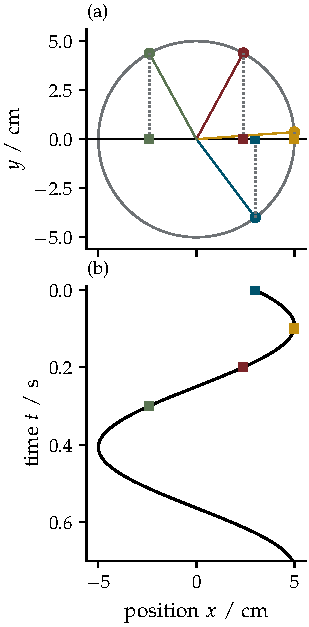
\includegraphics{ch04_oscillations/circle}
\caption{The oscillation as the shadow of a circle. A block with $\omega =
\SI{10}{\radian\per\second}$ starts \SI{3}{\centi\metre} out, moving
outwards at \SI{0.4}{\metre\per\second}. (a) The point $P$, going
anticlockwise round a circle of radius $A = \SI{5}{\centi\metre}$ from
$\phi = \SI{-0.927}{\radian}$, at $t = 0$, 0.1, 0.2 and \SI{0.3}{\second}
(dots), and its shadow on the $x$ axis (squares), one colour per moment.
(b) The shadow's position against time, with time running downwards so
that each square lies directly below the square of the same colour in
panel (a).}
\label{fig:os-circle}
\end{figure}

\subsection*{An example}

Take the block of \cref{sec:ne-spring}, with $m = \SI{0.5}{\kilogram}$
and $k = \SI{50}{\newton\per\metre}$, so that $\omega =
\SI{10}{\radian\per\second}$, started \SI{3}{\centi\metre} from its
resting place and moving outwards at \SI{0.4}{\metre\per\second}. That
section found $A = \SI{5}{\centi\metre}$, $\cos\phi = x(0)/A = 0.6$ and
$\phi = \arcsin(-0.8) = \SI{-0.927}{\radian}$. On the reference circle,
$P$ starts \SI{0.927}{\radian}, or $0.927\times\ang{180}/\pi =
\ang{53.1}$, below the positive $x$ axis, where
its shadow is at $A\cos\phi = 5\times0.6 = \SI{3}{\centi\metre}$. Moving
anticlockwise, $P$ climbs towards the axis, so the shadow moves outwards,
as the block does. $P$ reaches the axis when $\omega t + \phi = 0$, at $t
= 0.927/10 = \SI{0.0927}{\second}$, and there the block turns back, at
$x = A = \SI{5}{\centi\metre}$.

$P$ goes once round the circle while $\omega t$ grows by $2\pi$, so the
period is $2\pi/\omega = 2\pi/10 = \SI{0.628}{\second}$, and the
frequency, the number of oscillations per second (\cref{sec:mo-trig}),
is
\begin{equation*}
   \nu = \frac{\omega}{2\pi} = \frac{10}{2\pi} = \SI{1.592}{\hertz} ,
\end{equation*}
written with the Greek letter nu. The angular frequency $\omega$ is the
rate at which $P$ turns, in radians per second, and is $2\pi$ times the
frequency because each oscillation is one full turn of $2\pi$ radians.

\begin{selfcheck}
A block oscillates with $\omega = \SI{10}{\radian\per\second}$ and $A =
\SI{5}{\centi\metre}$. Where is the block, and which way and how fast is
it moving, when the angle $\omega t + \phi$ of its point $P$ equals
$\pi/2$?
\end{selfcheck}

%=============================================================================!
% 4.2  ENERGY IN THE OSCILLATOR                                               !
%=============================================================================!
\section{Energy in the oscillator}
\label{sec:os-energy}

An oscillating block has its largest kinetic energy at the centre of the
swing and none at the ends, and its potential energy does the opposite.
This section follows the trade and shows that, averaged over a period,
the energy is shared equally between the two forms, a result that
returns when Chapter~12 relates kinetic energy to temperature.

\subsection*{The trade}

With $x = A\cos(\omega t + \phi)$ and $v = -A\omega\sin(\omega t + \phi)$
(\cref{sec:os-circle}), and writing $\theta = \omega t + \phi$ for short,
the two energies of \cref{sec:en-potential} are
\begin{align*}
   K &= \tfrac12 m v^2 = \tfrac12 m A^2\omega^2\sin^2\theta
      = \tfrac12 k A^2\sin^2\theta
      && \text{since $\omega^2 = k/m$ gives $m\omega^2 = k$,}\\
   U &= \tfrac12 k x^2 = \tfrac12 k A^2\cos^2\theta .
\end{align*}
Taking out the common factor $\frac12 kA^2$ and using $\sin^2\theta +
\cos^2\theta = 1$, their sum is $E = \frac12 kA^2(\sin^2\theta +
\cos^2\theta) = \frac12 kA^2$, constant, as \cref{prop:en-energy-1d} requires. The energy
therefore fixes the amplitude, $A = \sqrt{2E/k}$: an oscillation with four
times the energy swings twice as far. For the same block
released instead from rest \SI{4}{\centi\metre} out, as in
\cref{fig:ne-spring}, $E =
\frac12\times50\times0.04^2 = \SI{0.04}{\joule}$. At $x =
\SI{2}{\centi\metre}$ the potential energy is $\frac12\times50\times0.02^2
= \SI{0.01}{\joule}$, and the remaining \SI{0.03}{\joule} is kinetic
(\cref{fig:os-energy}b). As the block swings, $K$ and $U$ rise and fall
twice in every period. By \cref{eq:mo-addition} with $\cos\pi = -1$ and
$\sin\pi = 0$, $\sin(\theta + \pi) = -\sin\theta$ and $\cos(\theta + \pi)
= -\cos\theta$, and squaring removes the minus signs, so $\sin^2\theta$
and $\cos^2\theta$ repeat when $\theta$ grows by $\pi$, half a turn
(\cref{fig:os-energy}a).

\begin{figure}[htb]
\centering
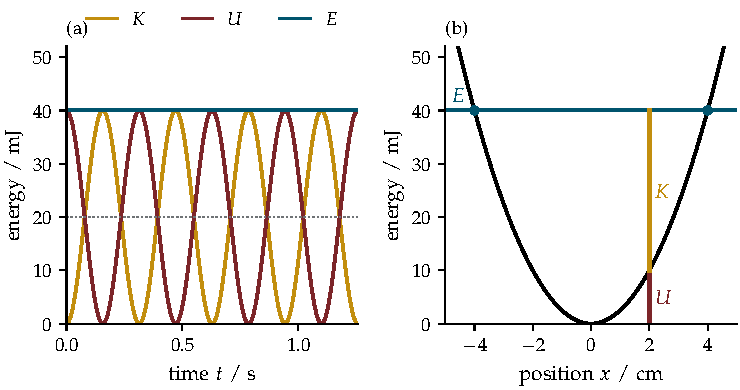
\includegraphics{ch04_oscillations/energy}
\caption{Energy in the oscillator: the block of \cref{sec:os-circle},
released instead from rest \SI{4}{\centi\metre} out, so that $E =
\SI{0.04}{\joule}$. (a) Kinetic energy $K$, potential energy $U$ and
their sum against time over two periods; the dotted line is $E/2$, the
average of each. (b) The energy diagram, $U = \frac12 kx^2$ with the line
$E$; at $x = \SI{2}{\centi\metre}$ the energy splits into $U =
\SI{0.01}{\joule}$ and $K = \SI{0.03}{\joule}$, and the dots mark the
turning points.}
\label{fig:os-energy}
\end{figure}

\Needspace{16\baselineskip}
\subsection*{Equal shares on average}

\begin{toolbox}[The average of a function]
The average of $n$ numbers is their sum divided by $n$. To average a
function $f(t)$ over an interval from $0$ to $t_1$, sample it at $n$ equally
spaced times $t_k$, a step $\tau = t_1/n$ apart, and average the
samples:
\begin{equation*}
   \frac1n\sum_{k} f(t_k) = \frac{1}{t_1}\sum_k f(t_k)\,\tau
   \;\longrightarrow\; \frac{1}{t_1}\int_0^{t_1} f(t)\,\dd t
   \qquad\text{as } n \to \infty ,
\end{equation*}
the first step multiplying and dividing by $\tau$ and using $n\tau = t_1$, the second the definition of the integral as a limit of such
sums (\cref{sec:mo-integrating}). The average of $f$ over the interval is
therefore $\frac{1}{t_1}\int_0^{t_1} f\,\dd t$, the area under its graph divided by
the length of the interval. We write it with an overbar, $\overline{f}$.
\end{toolbox}

To average $\cos^2\theta$ over a period, rewrite it. The addition formula
of \cref{sec:mo-trig} with both angles equal to $\theta$ gives
$\cos2\theta = \cos^2\theta - \sin^2\theta$, and
\begin{align*}
   \cos 2\theta &= \cos^2\theta - (1 - \cos^2\theta) = 2\cos^2\theta - 1
      && \text{replacing $\sin^2\theta$,}\\
   \cos^2\theta &= \tfrac12 + \tfrac12\cos 2\theta
      && \text{adding 1 to both sides and halving.}
\end{align*}
The second term averages to zero over a period, $t_1 = 2\pi/\omega$. With
$\theta = \omega t + \phi$, so that $2\theta = 2\omega t + 2\phi$, the
function $\sin(2\omega t + 2\phi)/(2\omega)$ has derivative $\cos(2\omega
t + 2\phi)$ by the chain rule, so the fundamental theorem of calculus
(\cref{sec:mo-integrating}) turns the integral into the change in that
function,
\begin{equation*}
   \int_0^{t_1} \cos(2\omega t + 2\phi)\,\dd t
   = \frac{\sin(2\omega t_1 + 2\phi) - \sin 2\phi}{2\omega} = 0 ,
\end{equation*}
because $2\omega t_1 = 4\pi$, two whole turns, after which the sine takes
its old value. Averaging the two terms of $\cos^2\theta$ separately,
\begin{align*}
   \overline{\cos^2\theta}
   &= \frac{1}{t_1}\int_0^{t_1}\tfrac12\,\dd t
      + \frac{1}{t_1}\int_0^{t_1}\tfrac12\cos(2\omega t + 2\phi)\,\dd t
      && \text{the integral of a sum,}\\
   &= \frac{1}{t_1}\times\frac{t_1}{2} + 0 = \frac12
      && \text{a rectangle, and the integral above,}
\end{align*}
and, since $\sin^2\theta = 1 - \cos^2\theta$, the same steps give
$\overline{\sin^2\theta} = 1 - \frac12 = \frac12$. The trade above gave
$K = E\sin^2\theta$ and $U = E\cos^2\theta$, with $E$ a constant that
comes outside each integral, so
\begin{equation}
   \overline{K} = \overline{U} = \tfrac12 E :
   \label{eq:os-equal-shares}
\end{equation}
over a period, a harmonic oscillator holds half its energy as kinetic
energy and half as potential energy. For the block, each averages
\SI{0.02}{\joule}, the dotted line of \cref{fig:os-energy}(a).

\notebook{04}{the spring with an animation, energy bars and its phase
portrait}

\begin{selfcheck}
At which positions does the block of \cref{fig:os-energy} have equal
kinetic and potential energy?
\end{selfcheck}

%=============================================================================!
% 4.3  THE PHASE PORTRAIT                                                     !
%=============================================================================!
\section{The phase portrait}
\label{sec:os-phase}

\Cref{sec:ne-equations} showed that the state of a body moving along a
line is the pair $(x, v)$, and drew motions as paths through the plane of
states (\cref{fig:ne-state}b). This plane is called the phase plane, and a
drawing of the paths through it the phase portrait of the system. For the
oscillator, energy alone gives the shape of every path.

\subsection*{Ellipses of constant energy}

Along any motion of the block, $\frac12 mv^2 + \frac12 kx^2 = E$. Dividing
both sides by $E$, which is positive unless the block rests at $x = 0$,
gives $kx^2/2E + mv^2/2E = 1$, and dividing the top and bottom of the
first fraction by $k$ and of the second by $m$,
\begin{equation}
   \frac{x^2}{2E/k} + \frac{v^2}{2E/m} = 1 ,
   \qquad\text{or}\qquad
   \Bigl(\frac{x}{a}\Bigr)^2 + \Bigl(\frac{v}{b}\Bigr)^2 = 1
   \quad\text{with } a = \sqrt{\frac{2E}{k}},\ b = \sqrt{\frac{2E}{m}} .
   \label{eq:os-ellipse}
\end{equation}
The second form says that the point $(x/a, v/b)$ lies on the circle of
radius 1, so the state $(x, v)$ lies on that circle stretched by the
factor $a$ along the $x$ axis and $b$ along the $v$ axis. A stretched
circle is an ellipse, and $a$ and $b$ are its semi-axes, half its width
and half its height. Here $a = \sqrt{2E/k}$ is the amplitude $A$
(\cref{sec:os-energy}), and $b = \sqrt{2E/m} = \sqrt{(2E/k)(k/m)} =
A\omega$, multiplying and dividing by $k$ under the root, is the largest
speed. For the block with $E =
\SI{0.04}{\joule}$ they are \SI{4}{\centi\metre} and
\SI{0.4}{\metre\per\second}.

\Cref{fig:os-phase}(a) draws the ellipses for three energies. Every
state lies on exactly one such ellipse, the one of its own energy, and the
block goes round it for ever, because energy is conserved. Two paths can
never cross: if they met at one state, that state would start two
different motions, which \cref{sec:ne-equations} rules out. The
direction of travel is clockwise: in the upper half of the plane $v > 0$,
so $x$ grows and the state moves to the right; in the lower half it moves
to the left. The panel is drawn with \SI{1}{\centi\metre} of position as
long as \SI{0.1}{\metre\per\second} of velocity, that is, with the velocity
divided by $\omega = \SI{10}{\radian\per\second}$, since
$\SI{0.1}{\metre\per\second}/\SI{10}{\radian\per\second} =
\SI{0.01}{\metre}$. On that scale the ellipses are circles, since $(x,
v/\omega) = A(\cos\theta, -\sin\theta)$ by \cref{sec:os-circle}: the
reference circle again, reflected in the $x$ axis, which reverses the sign
of the second coordinate and so turns the anticlockwise motion of $P$ into
a clockwise one.

\begin{figure}[htb]
\centering
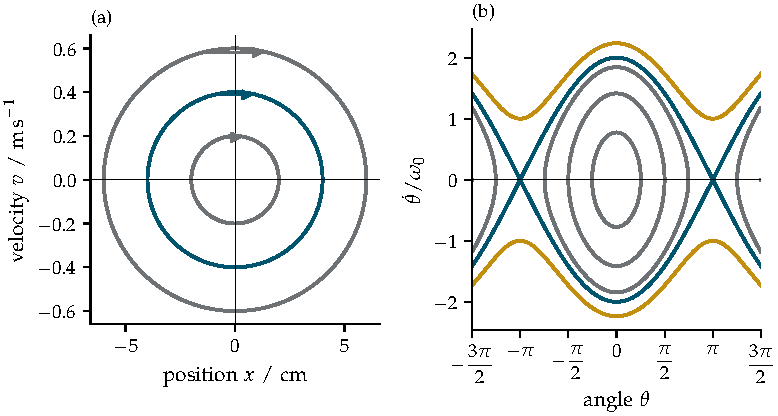
\includegraphics{ch04_oscillations/phase}
\caption{Phase portraits. (a) The block of \cref{sec:os-circle} at the
energies 0.01, 0.04 (teal) and \SI{0.09}{\joule}, traversed clockwise;
with \SI{1}{\centi\metre} drawn as long as \SI{0.1}{\metre\per\second}
the ellipses are circles. (b) The pendulum of \cref{sec:os-anharmonic},
with the rate of change of its angle, $\dot\theta$, in units of its
small-swing angular frequency $\omega_0$: closed paths while it swings (grey), the path through the
upright position (teal), and open paths when it goes over the top
(ochre).}
\label{fig:os-phase}
\end{figure}

Phase portraits return throughout the book. Chapter~7 uses momentum in
place of velocity and studies the flow of whole regions of the phase
plane, and Chapter~9 judges methods of computing motion by whether their
paths close, as these do, or spiral outwards. Panel (b), the pendulum,
belongs to \cref{sec:os-anharmonic}; there $\theta$ is the angle of the
pendulum, not $\omega t + \phi$. Its teal paths seem to cross at the
upright position, but that state is a path of its own, a pendulum
balanced at rest, which a pendulum on the teal paths approaches ever more
slowly and never reaches, so no state starts two motions.

\begin{selfcheck}
A block with $\omega = \SI{10}{\radian\per\second}$ starts at $x = 0$
with $v = \SI{0.3}{\metre\per\second}$. What are the semi-axes of its
ellipse in the phase plane, and where on the ellipse does it start?
\end{selfcheck}

%=============================================================================!
% 4.4  SMALL OSCILLATIONS ABOUT ANY MINIMUM                                   !
%=============================================================================!
\section{Small oscillations about any minimum}
\label{sec:os-small}

Wells are everywhere, springs far fewer: a pendulum hangs at
the bottom of a well of gravitational energy, and an atom sits at the
bottom of a well made by its neighbours. This section shows that small
swings about a minimum with positive curvature are approximately those
of a spring, and finds the stiffness
of that spring for a pendulum, for the bead of Chapter~3 and for a lithium
atom on the model surface.

\subsection*{The spring approximation near a minimum}

Let $U(x)$ have a minimum at $x_0$, with $U'(x_0) = 0$ and positive curvature,
$U''(x_0) > 0$. This last condition matters: a flatter minimum, such as
$U(x) = x^4$ at the origin, has no quadratic restoring term. The Taylor series of \cref{sec:mo-taylor}, with $x - x_0$ in the role
of the interval, gives
\begin{align*}
   U(x) &= U(x_0) + U'(x_0)\,(x - x_0) + \tfrac12 U''(x_0)\,(x - x_0)^2
      + \order{(x - x_0)^3}\\
   &= U(x_0) + \tfrac12 k\,(x - x_0)^2 + \order{(x - x_0)^3} ,
      \qquad k = U''(x_0) ,
\end{align*}
since $U'(x_0) = 0$. Near its bottom such a well is approximately a parabola, the
potential energy of a spring of stiffness $k = U''(x_0)$ stretched by $x -
x_0$; the constant $U(x_0)$ changes no force. As long as the swing is small
enough that the cubic and higher terms can be neglected, the motion is
simple harmonic, with
\begin{equation}
   \omega_0 = \sqrt{\frac{U''(x_0)}{m}} ,
   \label{eq:os-small}
\end{equation}
whatever the shape of the well further out. This is the result of
\cref{sec:en-diagrams}, now read from $U$ itself rather than from the
force, and the subscript 0 marks the angular frequency of small swings. How small is small enough, and what happens beyond, is the
subject of \cref{sec:os-anharmonic}.

\subsection*{Motion along a curved path}

A pendulum bob and a bead on a wire move along curves.
Measuring the position by the distance $s$ along the curve from its lowest
point, the speed is $\lvert\dd s/\dd t\rvert$ and the energy is $E =
\frac12 m\dot{s}^2 + U(s)$, where the dot denotes the rate of change with
time, as in \cref{sec:mo-acceleration}. Energy is conserved, because the push of
the rod or the wire is at right angles to the motion (\cref{sec:en-track}),
so differentiating $E$ with the chain rule,
\begin{equation*}
   0 = \frac{\dd E}{\dd t} = m\dot{s}\ddot{s} + \frac{\dd U}{\dd s}\,\dot{s}
   = \dot{s}\,\Bigl(m\ddot{s} + \frac{\dd U}{\dd s}\Bigr) .
\end{equation*}
Whenever the body is moving, $\dot{s} \neq 0$, and the bracket must vanish:
$m\ddot{s} = -\dd U/\dd s$, and since both sides change smoothly this
holds also at the instants when the body stops. Along its curve the body therefore moves as a
body on a line with potential energy $U(s)$, and \cref{eq:os-small}
applies with $s$ in place of $x$.

\subsection*{The pendulum}

A pendulum's bob, a small heavy weight of mass $m$, is fixed to a light
rigid rod of length $L$, light meaning that its own mass is negligible,
which turns freely about a pivot (\cref{fig:os-pendulum}). A rod, unlike
a string, can push as well as pull, so the bob stays on its circle even
above the pivot, as the large swings of \cref{sec:os-anharmonic} need.
When the rod makes an angle $\theta$ with the vertical, the bob has moved
$s = L\theta$ along its arc, by the definition of the radian
(\cref{sec:mo-trig}), and it is $L\cos\theta$ below the pivot, so
$L - L\cos\theta$ above its lowest point. Its potential energy is
therefore
\begin{equation*}
   U = mgL\,(1 - \cos\theta) = mgL\,\Bigl(1 - \cos\frac{s}{L}\Bigr) .
\end{equation*}
Differentiating twice with respect to $s$, by the chain rule,
\begin{equation*}
   \frac{\dd U}{\dd s} = mg\sin\frac{s}{L} , \qquad
   \frac{\dd^2 U}{\dd s^2} = \frac{mg}{L}\cos\frac{s}{L} ,
\end{equation*}
which is $mg/L$ at $s = 0$, since $\cos 0 = 1$, so by \cref{eq:os-small}
\begin{equation*}
   \omega_0 = \sqrt{\frac{g}{L}} .
\end{equation*}
The mass has cancelled, as in free fall. A pendulum \SI{1.2}{\metre} long
swings with $\omega_0 = \sqrt{9.80665/1.2} = \SI{2.859}{\radian\per
\second}$ and a period of $2\pi/\omega_0 = \SI{2.198}{\second}$, for small
swings.

\begin{figure}[htb]
\centering
\begin{tikzpicture}[line cap=round, line join=round, scale=1.1,
   force/.style={-{Stealth[length=5pt]}, line width=1.0pt}]
   \fill[black!35] (-0.8,0.05) rectangle (0.8,0.15);
   \draw[black!40, dashed, line width=0.5pt] (0,0) -- (0,-2.6);
   \draw[line width=0.8pt] (0,0) -- ({2.4*sin(35)},{-2.4*cos(35)});
   \draw[black!50, line width=0.4pt] (0,-0.8) arc[start angle=-90,
      end angle=-55, radius=0.8];
   \node at (0.2,-1.05) {\small $\theta$};
   \node[above right] at ({1.2*sin(35)},{-1.2*cos(35)}) {\small $L$};
   \draw[accent, line width=0.9pt] (0,-2.4) arc[start angle=-90,
      end angle=-55, radius=2.4];
   \node[accent, below] at (0.7,-2.42) {\small $s = L\theta$};
   \fill[black!15, draw=black, line width=0.5pt]
      ({2.4*sin(35)},{-2.4*cos(35)}) circle (0.12);
   \draw[black!40, line width=0.4pt] ({2.4*sin(35)+0.25},{-2.4*cos(35)})
      -- (1.9,{-2.4*cos(35)});
   \draw[black!40, line width=0.4pt] (0.15,-2.4) -- (1.9,-2.4);
   \draw[{Stealth[length=3pt]}-{Stealth[length=3pt]}, line width=0.4pt]
      (1.8,-2.4) -- (1.8,{-2.4*cos(35)})
      node[midway, right] {\small $L - L\cos\theta$};
\end{tikzpicture}
\caption{A pendulum, a bob on a light rod of length $L$, at the angle $\theta$. The bob has moved
$s = L\theta$ along its arc (teal) and has risen $L - L\cos\theta$ above
its lowest point.}
\label{fig:os-pendulum}
\end{figure}

\subsection*{The bead in its valley}

The bead of \cref{sec:en-track} has $U = mg\,h(x)$, but it moves along the
wire, so we need $\dd^2U/\dd s^2$ at the bottom of a valley, not $\dd^2U/
\dd x^2$. By the chain rule, with $x$ a function of $s$,
\begin{equation*}
   \frac{\dd U}{\dd s} = \frac{\dd U}{\dd x}\frac{\dd x}{\dd s} , \qquad
   \frac{\dd^2 U}{\dd s^2} = \frac{\dd^2 U}{\dd x^2}
   \Bigl(\frac{\dd x}{\dd s}\Bigr)^2 + \frac{\dd U}{\dd x}\frac{\dd^2 x}{\dd
   s^2} ,
\end{equation*}
the second by the product rule. At the bottom of a valley the wire is
level, so $\dd U/\dd x = 0$ and a short step along the wire is a step along
$x$, $\dd x/\dd s = 1$. Hence $\dd^2U/\dd s^2 = mg\,h''(x_0)$ there, and
$\omega_0 = \sqrt{g\,h''(x_0)}$. The deep valley lies at $x_0 =
\SI{-1.473}{\metre}$ (\cref{sec:en-diagrams}), where $h'' = 1.8\times
1.473^2 - 1.2 = \SI{2.7055}{\per\metre}$, so $\omega_0 =
\sqrt{9.80665\times2.7055} = \SI{5.151}{\radian\per\second}$, a period of
$2\pi/5.151 = \SI{1.220}{\second}$.

\subsection*{A lithium atom in a hollow}

On the model surface of \cref{sec:en-surface}, take the line through a
hollow and a bridge, the $x$ axis, along which a hop runs. There $\vb{r} =
(x, 0)$, and the three products in \cref{eq:en-surface} are $\vb{g}_1\cdot
\vb{r} = \lvert\vb{g}\rvert x\cos\ang{-30} = 2\pi x/a$, using
$\lvert\vb{g}\rvert = 4\pi/(\sqrt3\,a)$ and $\cos\ang{-30} = \sqrt3/2$;
$\vb{g}_2\cdot\vb{r} = 0$; and $\vb{g}_3\cdot\vb{r} = -2\pi x/a$. Since
the cosine is even and $\cos 0 = 1$,
\begin{equation}
   U(x, 0) = \frac{U_{\mathrm b}}{4}\Bigl[3 - 2\cos\frac{2\pi x}{a} - 1\Bigr]
   = \frac{U_{\mathrm b}}{2}\Bigl(1 - \cos\frac{2\pi x}{a}\Bigr) ,
   \label{eq:os-hop}
\end{equation}
a well of the same shape as the pendulum's. Differentiating twice by the
chain rule, as for the pendulum with $s/L$ replaced by $2\pi x/a$, gives
$U'' = \frac12 U_{\mathrm b}(2\pi/a)^2\cos(2\pi x/a)$, and $\cos 0 = 1$, so
\begin{equation*}
   k = U''(0) = \frac{U_{\mathrm b}}{2}\Bigl(\frac{2\pi}{a}\Bigr)^2
   = \frac{2\pi^2U_{\mathrm b}}{a^2}
   = \frac{19.7392\times0.3}{6.0516}
   = \SI{0.97854}{\electronvolt\per\angstrom\squared}
\end{equation*}
with $U_{\mathrm b} = \SI{0.3}{\electronvolt}$ and $a =
\SI{2.46}{\angstrom}$.
The force in \si{\electronvolt\per\angstrom} divided by the mass in
\si{\amu} becomes an acceleration in \si{\angstrom\per\femto\second
\squared} on multiplying by \num{9.648533e-3} (\cref{sec:ne-atoms}), so
for lithium, $\omega_0 = \sqrt{0.97854\times\num{9.648533e-3}/6.94} =
\SI{0.036884}{\radian\per\femto\second}$, and the period is $2\pi/\omega_0
= \SI{170.3}{\femto\second}$. The model is illustrative, but the scale is
the point: an atom rattles in its site a few times in a picosecond.
\Cref{ex:os-isotropic} shows that the well has the same curvature along
$y$ as along $x$.

\begin{keyidea}
Near a minimum with $U''(x_0) > 0$, $U \approx U(x_0) + \frac12
U''(x_0)(x - x_0)^2$: small swings are approximately those of a spring of stiffness
$U''(x_0)$, with angular frequency $\sqrt{U''(x_0)/m}$.
\end{keyidea}

\begin{selfcheck}
A pendulum is made four times as long. What happens to the period of its
small swings? Does the mass of the bob matter?
\end{selfcheck}

%=============================================================================!
% 4.5  LARGER SWINGS: ANHARMONIC WELLS                                        !
%=============================================================================!
\section{Larger swings: anharmonic wells}
\label{sec:os-anharmonic}

Real wells are not parabolas. The pendulum's well rises ever more slowly
than its parabola as the bob swings towards the horizontal, and the well that holds two atoms together
rises steeply when they are pushed together but levels off when they are
pulled apart. A well that is not a parabola is called anharmonic. This
section computes the period of a swing of any size from the energy alone,
and finds that in every well of interest here it grows with the energy.

\subsection*{The period from the energy}

\Cref{sec:en-track} noted that energy fixes the time of a journey through
the speed: a short step $\dd x$ taken at speed $v$ lasts $\dd x/v$. In a
well, with total energy $E$ and turning points $x_1 < x_2$, the speed at
$x$ is $v(x) = \sqrt{2(E - U(x))/m}$, so the journey from $x_1$ to $x_2$
takes $\int_{x_1}^{x_2}\dd x/v(x)$. The way back takes as long, since the
speed at each point is the same in either direction, and the period is
\begin{equation}
   \mathcal{T}(E) = 2\int_{x_1}^{x_2}\frac{\dd x}{\sqrt{2\bigl(E - U(x)\bigr)/m}} .
   \label{eq:os-period}
\end{equation}
At the turning points the speed is zero and the integrand is infinite.
The integral then means the limit as its ends approach the turning
points, and it is finite when, as in the harmonic case below, the
function whose derivative is the integrand tends to finite values there. To evaluate it we need
the derivative of the arcsine.

\begin{toolbox}[The derivative of an inverse function]
For $u$ between $-1$ and 1, $\theta = \arcsin u$ is the angle between
$-\pi/2$ and $\pi/2$ whose sine is $u$ (\cref{sec:mo-trig}), so $\sin
\theta(u) = u$ for every such $u$. Differentiating both sides with respect
to $u$, the left by the chain rule,
\begin{equation*}
   \cos\theta\,\frac{\dd\theta}{\dd u} = 1 ,
   \qquad\text{so}\qquad
   \frac{\dd}{\dd u}\arcsin u = \frac{1}{\cos\theta}
   = \frac{1}{\sqrt{1 - u^2}} ,
\end{equation*}
since $\cos\theta = +\sqrt{1 - \sin^2\theta}$ for an angle between
$-\pi/2$ and $\pi/2$, where the cosine is not negative. With $u = x/A$ and
the chain rule, $\dd u/\dd x = 1/A$, so
\begin{equation*}
   \frac{\dd}{\dd x}\arcsin\frac{x}{A} = \frac{1}{A}\,
   \frac{1}{\sqrt{1 - x^2/A^2}} = \frac{1}{\sqrt{A^2\,(1 - x^2/A^2)}}
   = \frac{1}{\sqrt{A^2 - x^2}} ,
\end{equation*}
the positive $A$ having gone inside the root as $A^2$.
The same method, differentiating the equation that defines the inverse,
gives the derivative of any inverse function.
\end{toolbox}

For the spring, $U = \frac12 kx^2$ and $E = \frac12 kA^2$, so $E - U =
\frac12 k(A^2 - x^2)$ and $v = \omega\sqrt{A^2 - x^2}$. Then
\begin{align*}
   \mathcal{T} &= \frac{2}{\omega}\int_{-A}^{A}\frac{\dd x}{\sqrt{A^2 - x^2}}
   = \frac{2}{\omega}\Bigl[\arcsin\frac{x}{A}\Bigr]_{-A}^{A}
      && \text{by the toolbox and \cref{eq:mo-integrals}}\\
   &= \frac{2}{\omega}\Bigl(\frac{\pi}{2} - \Bigl(-\frac{\pi}{2}\Bigr)\Bigr)
   = \frac{2\pi}{\omega} ,
\end{align*}
the period of \cref{sec:os-circle}, whatever the amplitude. The integrand
is infinite at $\pm A$, yet $\arcsin(x/A)$ rises only to $\pm\pi/2$ there,
so the area under it is finite: the spike is tall but very narrow. For
other wells the integral is evaluated by computer. The function
\texttt{oscillators.period} of \texttt{mdlab} finds the turning points,
then writes $x = c - \eta\cos\vartheta$, with $c$ the centre and $\eta$ the
half-width of the allowed region, so that $\vartheta$ runs from 0 at
$x_1$ to $\pi$ at $x_2$. A short step $\dd\vartheta$ moves $x$ by $\dd x =
\eta\sin\vartheta\,\dd\vartheta$, the derivative of $c - \eta\cos\vartheta$
times the step, so each time $\dd x/v$ becomes $\eta\sin\vartheta\,
\dd\vartheta/v$, and these are added up over $\vartheta$ from 0 to $\pi$.
Near $x_1$, where $U(x_1) = E$, the Taylor series gives $E - U(x) \approx
-U'(x_1)\,(x - x_1)$, and $x - x_1 = \eta(1 - \cos\vartheta) \approx \frac12
\eta\vartheta^2$, so $v$ grows in proportion to $\vartheta$; so does
$\sin\vartheta \approx \vartheta$, and their ratio, the new integrand,
stays finite, as it does near $x_2$. The integral over $\vartheta$ is
then evaluated by Gauss--Legendre quadrature, a weighted sum of the
integrand at chosen points, which converges quickly for a smooth
integrand. Its tests check it against the spring, against closed
forms for the pendulum and for the Morse well below, and against motions
timed by \texttt{solve\_newton}.

\subsection*{The pendulum and the hop}

The pendulum's well, $U = mgL(1 - \cos\theta)$, and the hop coordinate of
the lithium atom, \cref{eq:os-hop}, have the same shape,
\begin{equation*}
   U = \tfrac12 D\,\Bigl(1 - \cos\frac{2\pi x}{\Lambda}\Bigr) ,
\end{equation*}
a cosine well of depth $D$ that repeats every $\Lambda$: for the
pendulum $x$ is the distance $s = L\theta$ along the arc, $\Lambda =
2\pi L$ and $D = 2mgL$, the potential energy of the bob held upright; for the atom $\Lambda = a$ and $D = U_{\mathrm b}$,
the barrier. Away from its bottom the cosine well rises more slowly than
its parabola (\cref{fig:os-wells}a), so the restoring force there is
weaker than a spring's, and in a swing of the same amplitude the body
moves more slowly and takes longer. \Cref{eq:os-period} gives, for the pendulum,
\begin{center}
\begin{tabular}{lccccc}
\toprule
amplitude & \ang{10} & \ang{45} & \ang{90} & \ang{150} & \ang{179}\\
\midrule
period / small-swing period & 1.0019 & 1.0400 & 1.1803 & 1.7622 & 3.9011\\
\bottomrule
\end{tabular}
\end{center}
For swings of \ang{10} the period is within \SI{0.2}{\percent} of
$2\pi\sqrt{L/g}$, and it changes only slowly with the amplitude: a clock
whose swing grows from \ang{10} to \ang{11} loses about \SI{35}{\second} a
day, which is why clockmakers keep the swing small and steady. Beyond \ang{90} the bob
ends each swing above the pivot, where only a rod, which can push, keeps
it on its circle; a string would go slack. As the amplitude approaches
\ang{180}
the bob lingers ever longer near the top, where the force on it is
nearly zero, and the period grows without limit (\cref{fig:os-period}).

The lithium atom behaves the same way. With \SI{0.25}{\electronvolt} above
the bottom of the hollow,
below the \SI{0.3}{\electronvolt} barrier, it rattles in its hollow with a
period of \SI{253.8}{\femto\second}, half as long again as the
\SI{170.3}{\femto\second} of small swings, and with
\SI{0.297}{\electronvolt} the period is \SI{400.8}{\femto\second}. With exactly
the barrier as energy, the atom would creep ever more slowly towards the
bridge without ever reaching it. The phase
portrait of the cosine well (\cref{fig:os-phase}b) shows all of this at
once: closed paths for swings or rattles, the path through the top that
separates them from the open paths of a pendulum going over the top or an
atom hopping on from hollow to hollow.

\subsection*{Two wells for a pair of atoms}

The energy of two atoms depends on the distance $r$ between them, and two
standard shapes model it; Chapter~8 discusses where they apply. The Morse
well, used for a chemical bond, is
\begin{equation*}
   U_{\mathrm{M}}(r) = D\,\bigl(1 - \mathrm{e}^{-a(r - r_0)}\bigr)^2 ,
\end{equation*}
with three constants. At $r = r_0$ the exponential is 1 and $U_{\mathrm M}
= 0$, its least value, since it is a square; when the atoms are pulled
far apart the exponential vanishes and $U_{\mathrm M}$ levels off at $D$,
the energy needed to separate them; when they are pushed together,
$r < r_0$, the exponential grows rapidly and so does $U_{\mathrm M}$. The
constant $a$, an inverse length, sets the width of the well; here it is
not the spacing of the surface. Near the bottom, with $y = r - r_0$ and
the exponential series of \cref{sec:ne-drag}, $\mathrm{e}^{-ay} = 1 - ay +
\order{y^2}$, so $1 - \mathrm{e}^{-ay} = ay + \order{y^2}$ and, squaring,
\begin{equation*}
   U_{\mathrm M} = D a^2 y^2 + \order{y^3} ,
   \qquad\text{a spring of stiffness } k = 2Da^2 .
\end{equation*}

The Lennard-Jones well, often used for atoms that form no bond, such as those
of the noble gases (helium, neon, argon and their family, which hardly
react), is
\begin{equation*}
   U_{\mathrm{LJ}}(r) = 4\varepsilon\Bigl[\Bigl(\frac{\sigma}{r}\Bigr)^{12}
   - \Bigl(\frac{\sigma}{r}\Bigr)^6\Bigr] ,
\end{equation*}
a steep repulsion, $r^{-12}$, that dominates at short range and a weaker
attraction, $-r^{-6}$, that dominates at long range. The power rule of
\cref{sec:mo-velocity} was found for whole $n \ge 1$, but it holds for
$r^{-n} = 1/r^n$ too: differentiating $r^{-n}\,r^n = 1$ by the product
rule gives $r^n\,\dd(r^{-n})/\dd r + r^{-n}\,n r^{n-1} = 0$, so $\dd
(r^{-n})/\dd r = -n\,r^{-n-1}$. Differentiating with this rule,
\begin{equation*}
   \frac{\dd U_{\mathrm{LJ}}}{\dd r}
   = 4\varepsilon\Bigl[-12\,\frac{\sigma^{12}}{r^{13}}
   + 6\,\frac{\sigma^6}{r^7}\Bigr]
   = \frac{24\varepsilon}{r}\Bigl[\Bigl(\frac{\sigma}{r}\Bigr)^6
   - 2\Bigl(\frac{\sigma}{r}\Bigr)^{12}\Bigr] ,
\end{equation*}
which vanishes when the bracket, $(\sigma/r)^6\,[1 - 2(\sigma/r)^6]$,
does, so when $(\sigma/r)^6 = \frac12$, that is $(r/\sigma)^6 = 2$, at
$r_{\min} = 2^{1/6}\sigma = 1.1225\,\sigma$, where $U_{\mathrm{LJ}} = 4\varepsilon(\frac14 - \frac12)
= -\varepsilon$. Differentiating once more,
\begin{equation*}
   \frac{\dd^2 U_{\mathrm{LJ}}}{\dd r^2}
   = \frac{4\varepsilon}{r^2}\Bigl[156\Bigl(\frac{\sigma}{r}\Bigr)^{12}
   - 42\Bigl(\frac{\sigma}{r}\Bigr)^6\Bigr]
   = \frac{4\varepsilon}{r_{\min}^2}\Bigl[\frac{156}{4} - \frac{42}{2}\Bigr]
   = \frac{4\times18\,\varepsilon}{2^{1/3}\sigma^2}
   = 57.15\,\frac{\varepsilon}{\sigma^2}
\end{equation*}
at the minimum, the middle steps putting in $(\sigma/r)^{12} = \frac14$,
$(\sigma/r)^6 = \frac12$ and $r_{\min}^2 = 2^{2/6}\sigma^2 =
2^{1/3}\sigma^2$, with $39 - 21 = 18$.

\begin{figure}[htb]
\centering
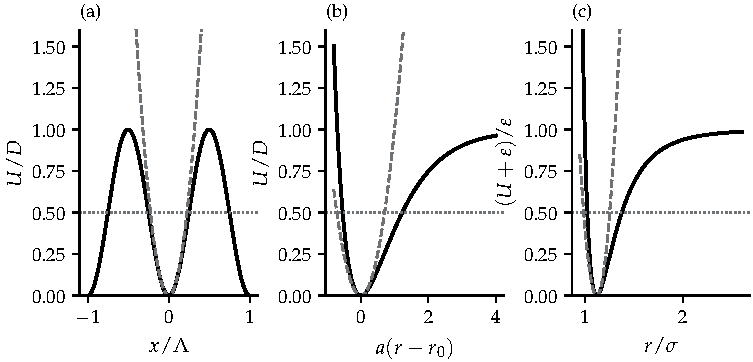
\includegraphics{ch04_oscillations/wells}
\caption{Three anharmonic wells (black) against the parabolas of the same
curvature at their bottoms (dashed), each in its own natural units; the
dotted lines mark half the depth. (a) The cosine well of the pendulum and
of the lithium hop. (b) The Morse well of a bond. (c) The Lennard-Jones
well, drawn from its bottom.}
\label{fig:os-wells}
\end{figure}

Both wells are lopsided (\cref{fig:os-wells}b, c): steeper than their
parabola on the inside, softer on the outside. A swing therefore reaches
less far in and much further out than a spring's would; in the
Lennard-Jones well with half the depth as energy, the turning points are
at $1.027\,\sigma$ and $1.377\,\sigma$, against $0.990\,\sigma$ and
$1.255\,\sigma$ for the parabola, whose turning points lie
$\sqrt{2\times0.5/57.15} = 0.132\,\sigma$ either side of the minimum at
$1.1225\,\sigma$. The soft outer side wins, and the period grows with the
energy (\cref{fig:os-period}). Measured from the bottom, at a tenth, half
and nine tenths of the depth the period is 1.054, 1.414 and 3.162 times
that of small swings for the Morse well, which are $1/\sqrt{1 - E/D}$
exactly, the closed form the tests use, and 1.069, 1.554 and 4.399 times
for the Lennard-Jones well. These ratios hold for any constants and any
mass, because in the units of the figures the wells have no constants
left, and by \cref{eq:os-period} every period is proportional to
$\sqrt m$. A bond with
more energy therefore vibrates more slowly, and the period of the small
swings, the one that sets the steps of a simulation, is the shortest.

\begin{figure}[htb]
\centering
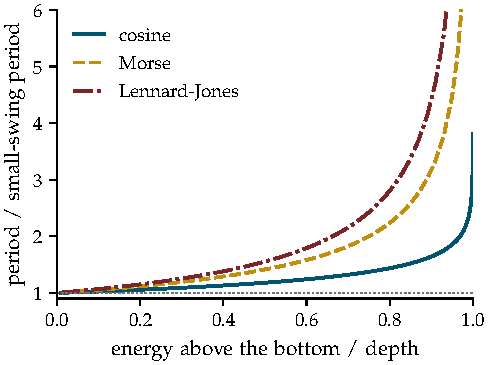
\includegraphics{ch04_oscillations/period}
\caption{The period of the motion in each well of \cref{fig:os-wells},
divided by the period of small swings, against the energy above the
bottom as a fraction of the depth, computed from \cref{eq:os-period}. The
cosine well's period grows without limit as the energy approaches the
barrier, though so slowly that it is only 3.8 at 0.9999 of the barrier,
where its curve stops; the others' grows without limit as the energy
approaches that needed to separate the atoms. A spring keeps the ratio 1 (dotted).}
\label{fig:os-period}
\end{figure}

\notebook{04}{explore the period in each well as the energy grows}

\begin{selfcheck}
Why does a pendulum swinging out to \ang{90} on each side take longer for
each swing than one swinging out to \ang{10}, even though it moves faster at the
bottom?
\end{selfcheck}

%=============================================================================!
% 4.6  DAMPING                                                                !
%=============================================================================!
\section{Damping}
\label{sec:os-damped}

A block on a spring in air swings for a long time; the same block in
honey creeps back to its resting place without swinging at all. This
section adds the drag of \cref{sec:ne-drag} to the spring and solves the
motion exactly, with one substitution that removes the drag from the
equation.

\subsection*{The equation and a substitution}

With the drag force $-bv$ of \cref{sec:ne-drag} added to the spring's
$-kx$, the second law reads $m\ddot{x} = -kx - b\dot{x}$, and dividing by
$m$,
\begin{equation}
   \ddot{x} = -\omega_0^2\,x - \gamma\,\dot{x} ,
   \qquad \omega_0 = \sqrt{\frac{k}{m}} , \quad \gamma = \frac{b}{m} ,
   \label{eq:os-damped}
\end{equation}
where $\omega_0$ is the angular frequency the block would have without
drag and $\gamma$ is the drag rate. The drag removes energy, so we expect
the swing to shrink, and we write
\begin{equation*}
   x(t) = \mathrm{e}^{-\gamma t/2}\,y(t) ,
\end{equation*}
which separates a shrinking factor from a new unknown $y$. The factor
$\frac12\gamma$ is chosen because it makes the drag term disappear, as we
now show. By the product rule and the chain rule, with $\dd\mathrm{e}^{
-\gamma t/2}/\dd t = -\frac12\gamma\,\mathrm{e}^{-\gamma t/2}$ by the
exponential toolbox of \cref{sec:ne-drag}, and for $\ddot{x}$ the product
rule applied to $\dot{x}$, the last step multiplying out the second
bracket and collecting the two terms in $\dot{y}$,
\begin{align*}
   \dot{x} &= \mathrm{e}^{-\gamma t/2}\bigl(\dot{y} - \tfrac12\gamma y\bigr) ,\\
   \ddot{x} &= \mathrm{e}^{-\gamma t/2}\bigl(\ddot{y} - \tfrac12\gamma\dot{y}\bigr)
      - \tfrac12\gamma\,\mathrm{e}^{-\gamma t/2}\bigl(\dot{y}
      - \tfrac12\gamma y\bigr)
   = \mathrm{e}^{-\gamma t/2}\bigl(\ddot{y} - \gamma\dot{y}
      + \tfrac14\gamma^2 y\bigr) .
\end{align*}
Putting these into \cref{eq:os-damped}, dividing by $\mathrm{e}^{-\gamma
t/2}$, which is never zero, and multiplying out the bracket on the right,
\begin{align*}
   \ddot{y} - \gamma\dot{y} + \tfrac14\gamma^2 y
   &= -\omega_0^2 y - \gamma\dot{y} + \tfrac12\gamma^2 y\\
   \ddot{y} &= -\omega_0^2 y + \tfrac12\gamma^2 y - \tfrac14\gamma^2 y
      && \text{adding $\gamma\dot{y} - \tfrac14\gamma^2 y$ to both sides}\\
   &= -\bigl(\omega_0^2 - \tfrac14\gamma^2\bigr)\,y .
\end{align*}
The terms in $\dot{y}$ have cancelled: $y$ obeys an equation without drag,
whose solution depends on the sign of $\omega_0^2 - \frac14\gamma^2$.

\subsection*{Three kinds of motion}

\emph{Light drag}, $\frac12\gamma < \omega_0$. Then $\omega_0^2 -
\frac14\gamma^2$ is positive, and $y$ is a spring with angular frequency
\begin{equation*}
   \omega_{\mathrm d} = \sqrt{\omega_0^2 - \tfrac14\gamma^2} ,
\end{equation*}
so $y = c_1\cos\omega_{\mathrm d}t + c_2\sin\omega_{\mathrm d}t$, as in
\cref{sec:ne-spring}, and
\begin{equation*}
   x(t) = \mathrm{e}^{-\gamma t/2}\bigl(c_1\cos\omega_{\mathrm d}t
   + c_2\sin\omega_{\mathrm d}t\bigr) :
\end{equation*}
an oscillation whose swing shrinks by the factor $\mathrm{e}^{-\gamma
t/2}$. Setting $t = 0$ gives $c_1 = x_0$, and the formula for $\dot{x}$
above gives $v_0 = \dot{y}(0) - \frac12\gamma x_0 = c_2\omega_{\mathrm d} -
\frac12\gamma x_0$, so $c_2 = (v_0 + \frac12\gamma x_0)/\omega_{\mathrm d}$.
The block of \cref{sec:os-circle}, with $\omega_0 =
\SI{10}{\radian\per\second}$, in a liquid with $\gamma =
\SI{4}{\per\second}$, swings with $\omega_{\mathrm d} = \sqrt{100 - 4} =
\SI{9.798}{\radian\per\second}$, a period of $2\pi/9.798 =
\SI{0.641}{\second}$, a little longer than the $2\pi/10 =
\SI{0.628}{\second}$ without drag. Its swing halves when $\mathrm{e}^{
-\gamma t/2} = 0.5$; taking the natural logarithm of both sides,
$-\frac12\gamma t = \ln 0.5 = -0.693$, so the swing halves every
$0.693/(\frac12\gamma) = \SI{0.347}{\second}$. This case is called under-damped.

\emph{Heavy drag}, $\frac12\gamma > \omega_0$. Then $\ddot{y} = \kappa^2
y$ with $\kappa = \sqrt{\frac14\gamma^2 - \omega_0^2}$. By the exponential
toolbox, $\mathrm{e}^{\kappa t}$ has second derivative $\kappa^2\mathrm{e}^{
\kappa t}$, and so has $\mathrm{e}^{-\kappa t}$, so $y = c_1\mathrm{e}^{
\kappa t} + c_2\mathrm{e}^{-\kappa t}$ and
\begin{equation*}
   x(t) = c_1\,\mathrm{e}^{-(\gamma/2 - \kappa)t}
   + c_2\,\mathrm{e}^{-(\gamma/2 + \kappa)t} .
\end{equation*}
Since $\kappa^2 = \frac14\gamma^2 - \omega_0^2$ is less than
$\frac14\gamma^2$, $\kappa < \frac12\gamma$, so both exponents are
negative and both terms die away. Multiplying $x = 0$ by $\mathrm{e}^{
(\gamma/2 + \kappa)t}$ gives $c_1\mathrm{e}^{2\kappa t} = -c_2$, which
holds at one instant at most, since $\mathrm{e}^{2\kappa t}$ never takes a
value twice: the block passes its resting place at most once and never
swings to and fro, but creeps back. This case is called
over-damped. With $\gamma = \SI{40}{\per\second}$, $\kappa = \sqrt{400 -
100} = \SI{17.32}{\per\second}$, and the slower term decays at only
$20 - 17.32 = \SI{2.68}{\per\second}$, so the creep is slow.

\emph{Critical drag}, $\frac12\gamma = \omega_0$. Then $\ddot{y} = 0$, so
$y = c_1 + c_2 t$ by two integrations, and $x = (c_1 + c_2t)\,\mathrm{e}^{
-\gamma t/2}$. Since $c_1 + c_2t$ is zero at one instant at most, this
critically damped motion passes the resting place at most once, and not
at all when released from rest, where $c_1 = x_0$ and, by the formula
for $\dot{x}$, $c_2 = \frac12\gamma x_0$, of the same sign.

For the block released from rest at $x_0 = \SI{0.04}{\metre}$, critical
drag, $\gamma = \SI{20}{\per\second}$, gives $c_2 = 10\times0.04 =
\SI{0.4}{\metre\per\second}$, and half a second after release the block
is $(0.04 + 0.4\times0.5)\,\mathrm{e}^{-5} = \SI{0.16}{\centi\metre}$ out.
With $\gamma = \SI{40}{\per\second}$, $y(0) = c_1 + c_2 = 0.04$ and, since
$\dot{x}(0) = \dot{y}(0) - \frac12\gamma x_0 = 0$, $\dot{y}(0) =
\kappa(c_1 - c_2) = \frac12\gamma x_0 = 0.8$; these give $c_1 =
\SI{0.0431}{\metre}$ and $c_2 = \SI{-0.0031}{\metre}$, and at half a
second $x = 0.0431\,\mathrm{e}^{-2.68\times0.5} = \SI{1.13}{\centi
\metre}$, the second term being negligible. The critically damped block
returns sooner (\cref{fig:os-damped}).

In each case two constants match any starting position and velocity, so by
the uniqueness of solutions (\cref{sec:ne-equations}) these formulas are
the motion. The energy falls throughout, at the rate $-bv^2$ of
\cref{sec:en-friction}.

\begin{figure}[htb]
\centering
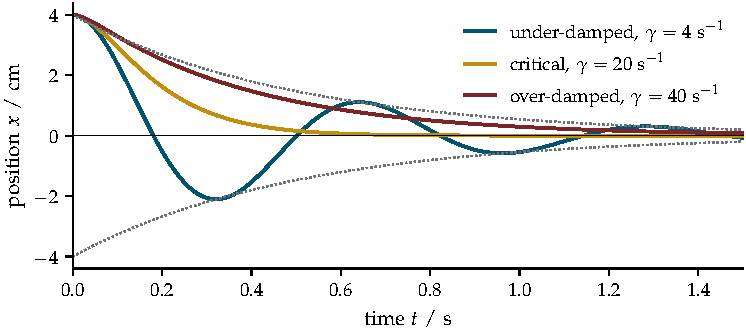
\includegraphics{ch04_oscillations/damped}
\caption{The block of \cref{sec:os-circle}, with $\omega_0 =
\SI{10}{\radian\per\second}$, released from rest \SI{4}{\centi\metre} out
in liquids with three drag rates. The under-damped block turns back on
the dotted curves $\pm\SI{4}{\centi\metre}\times\mathrm{e}^{-\gamma t/2}$;
the critically damped one returns without swinging past zero; the
over-damped one creeps back more slowly.}
\label{fig:os-damped}
\end{figure}

Chapter~13 adds this drag to the motion of atoms, together with
random kicks that make up for the energy it removes, to hold a simulation
at a chosen temperature; the drag rate $\gamma$ there plays the same role
as here.

\begin{selfcheck}
For the block with $\omega_0 = \SI{10}{\radian\per\second}$, what drag rate
makes the motion critically damped? With $\gamma = \SI{8}{\per\second}$,
what is the period of the swing?
\end{selfcheck}

%=============================================================================!
% 4.7  DRIVING AND RESONANCE                                                  !
%=============================================================================!
\section{Driving and resonance}
\label{sec:os-driven}

A child on a swing, pushed gently at just the right moment of each swing,
soon swings high; the same pushes at the wrong rhythm achieve little. This
section drives the damped oscillator with a force that rises and falls as
a sinusoid and finds how the size of the response depends on the rhythm of
the push.

\subsection*{The steady response}

Add to the block of \cref{sec:os-damped} a force $F_0\cos\omega t$, where
$\omega$ is now the angular frequency of the push, chosen freely, and
$\omega_0$ remains that of the spring alone. The second law becomes
$m\ddot{x} = -kx - b\dot{x} + F_0\cos\omega t$; dividing by $m$, writing
$f = F_0/m$ and moving the spring and drag terms to the left,
\begin{equation}
   \ddot{x} + \gamma\dot{x} + \omega_0^2 x = f\cos\omega t .
   \label{eq:os-driven}
\end{equation}
After the start has been forgotten, we expect the block to swing in step
with the push, at the same angular frequency but lagging behind it, so we
try
\begin{equation*}
   x = A\cos(\omega t - \delta) ,
\end{equation*}
with an amplitude $A$ and a lag $\delta$ to be found. Writing $\psi =
\omega t - \delta$ for short, the chain rule with $\dd\psi/\dd t = \omega$
gives $\dot{x} = -A\omega\sin\psi$ and $\ddot{x} = -A\omega^2\cos\psi$,
so the left side of \cref{eq:os-driven} is
\begin{equation*}
   A\bigl(\omega_0^2 - \omega^2\bigr)\cos\psi - A\gamma\omega\sin\psi .
\end{equation*}
On the right, $\omega t = \psi + \delta$, and the addition formula of
\cref{sec:mo-trig} gives $f\cos\omega t = f\cos\delta\cos\psi - f\sin
\delta\sin\psi$. Both sides are now combinations of $\cos\psi$ and $\sin
\psi$, and they must agree at every instant. At the instants when $\psi$
is a whole number of turns, $\cos\psi = 1$ and $\sin\psi = 0$; at those a
quarter turn later, $\cos\psi = 0$ and $\sin\psi = 1$. Comparing the two
sides at these instants,
\begin{equation*}
   A\bigl(\omega_0^2 - \omega^2\bigr) = f\cos\delta , \qquad
   A\gamma\omega = f\sin\delta .
\end{equation*}
Squaring both, adding them and using $\cos^2\delta + \sin^2\delta = 1$
gives $A^2[(\omega_0^2 - \omega^2)^2 + \gamma^2\omega^2] = f^2$, and
dividing the second equation by the first gives $\tan\delta$:
\begin{equation}
   A = \frac{f}{\sqrt{\bigl(\omega_0^2 - \omega^2\bigr)^2 + \gamma^2\omega^2}} ,
   \qquad
   \tan\delta = \frac{\gamma\omega}{\omega_0^2 - \omega^2} .
   \label{eq:os-resonance}
\end{equation}
Since $\sin\delta = A\gamma\omega/f$ is positive, $\delta$ lies between 0
and $\pi$: the block always lags behind the push. Below resonance, where
$\omega < \omega_0$, $\cos\delta$ is positive too, and $\delta =
\arctan\bigl(\gamma\omega/(\omega_0^2 - \omega^2)\bigr)$ lies between 0
and $\pi/2$, inside the range of the arctangent. Above it $\cos\delta$ is
negative and $\delta$ lies between $\pi/2$ and $\pi$; since $\pi -
\delta$ has the same sine as $\delta$ and the opposite cosine
(\cref{sec:mo-trig}), $\tan(\pi - \delta) = -\tan\delta$, and $\delta =
\pi - \arctan\bigl(\gamma\omega/(\omega^2 - \omega_0^2)\bigr)$.

This is one motion that obeys \cref{eq:os-driven}, but it does not start
from an arbitrary position and velocity. Adding to it any motion $x_{\mathrm
h}$ of the undriven damped block, for which $\ddot{x}_{\mathrm h} + \gamma
\dot{x}_{\mathrm h} + \omega_0^2x_{\mathrm h} = 0$, gives another, since
the derivative of a sum is the sum of the derivatives: putting $x +
x_{\mathrm h}$ into the left side of \cref{eq:os-driven} gives the left
side for $x$, which is $f\cos\omega t$, plus that for $x_{\mathrm h}$,
which is zero. The two constants of $x_{\mathrm h}$ (\cref{sec:os-damped})
can match any starting state, so by the uniqueness of solutions
(\cref{sec:ne-equations}) every driven motion is the steady response plus
a damped motion, and the damped part dies away, as $\mathrm{e}^{-\gamma
t/2}$ for light drag.
Combining solutions by adding them works only because \cref{eq:os-driven}
contains $x$ and its derivatives to the first power alone; such an
equation is called linear.

\subsection*{Resonance}

The amplitude is largest when the denominator of \cref{eq:os-resonance} is
smallest, which, for light drag, is close to $\omega = \omega_0$, where the
first term vanishes. Driving a system at its own angular frequency is
called driving it at resonance. There $\omega_0^2 - \omega^2 = 0$, so the
first of the two equations above gives $\cos\delta = 0$; with $\sin\delta$
positive, $\delta = \pi/2$ and $\sin\delta = 1$, and the second gives
$A\gamma\omega_0 = f$:
\begin{equation*}
   A = \frac{f}{\gamma\omega_0} , \qquad \delta = \frac{\pi}{2} .
\end{equation*}
Push the block of \cref{sec:os-circle}, with $m = \SI{0.5}{\kilogram}$,
$k = \SI{50}{\newton\per\metre}$ and so $\omega_0 =
\SI{10}{\radian\per\second}$, with a force of amplitude
\SI{0.5}{\newton}, so that $f = 0.5/0.5 = \SI{1}{\metre\per\second
\squared}$. Held still, that force would stretch the spring by $F_0/k =
0.5/50 = \SI{1}{\centi\metre}$, which is also the amplitude for a very slow
push, $\omega \to 0$, where $A \to f/\omega_0^2 = (F_0/m)/(k/m) =
F_0/k$. At resonance, with
$\gamma = \SI{2}{\per\second}$, the amplitude is $1/(2\times10) =
\SI{5}{\centi\metre}$, five times larger; with $\gamma =
\SI{1}{\per\second}$ it is \SI{10}{\centi\metre}, and with $\gamma =
\SI{4}{\per\second}$, \SI{2.5}{\centi\metre} (\cref{fig:os-resonance}a).
The ratio of the amplitude at resonance to that for a very slow push,
$\bigl(f/(\gamma\omega_0)\bigr)\big/\bigl(f/\omega_0^2\bigr) =
\omega_0/\gamma$, is called the quality factor of the oscillator: the
lighter the drag, the higher and narrower the peak. The peak's width,
measured where $A$ exceeds its largest value divided by $\sqrt2$, is close
to $\gamma$. Near the peak, $\omega_0^2 - \omega^2 = (\omega_0 -
\omega)(\omega_0 + \omega) \approx 2\omega_0(\omega_0 - \omega)$ and
$\gamma\omega \approx \gamma\omega_0$, so the square root in
\cref{eq:os-resonance} is about $\omega_0\sqrt{4(\omega_0 - \omega)^2 +
\gamma^2}$, which is $\sqrt2$ times its value at $\omega_0$ when
$4(\omega_0 - \omega)^2 = \gamma^2$, at $\omega = \omega_0 \pm
\frac12\gamma$, a distance $\gamma$ apart. Solved exactly by computer, the
widths are 1.00, 2.02 and \SI{4.19}{\radian\per\second} for $\gamma = 1$,
2 and \SI{4}{\per\second}.

The lag explains why the rhythm matters (\cref{fig:os-resonance}b). At
resonance $\delta = \pi/2$: the block is at the centre of its swing,
moving fastest, when the push is strongest, so the push always acts along
the velocity and its power $F v$ is never negative. Pushed slowly, the
block follows the push, $\delta \to 0$; pushed fast, it moves against it,
$\delta \to \pi$, and in both cases the push spends half of each cycle
working against the motion.

\begin{figure}[htb]
\centering
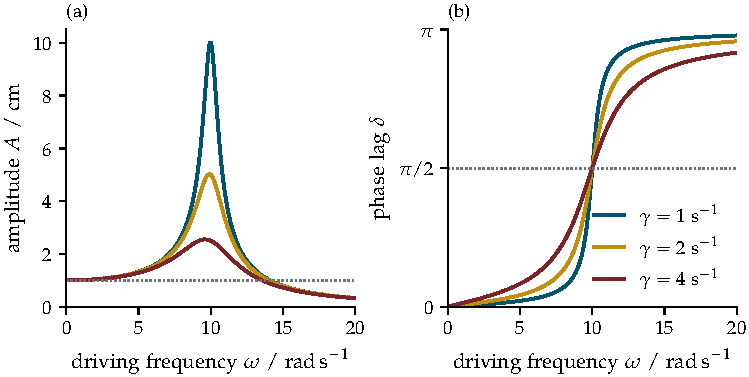
\includegraphics{ch04_oscillations/resonance}
\caption{The block of \cref{sec:os-circle} driven by a force of amplitude
\SI{0.5}{\newton} at angular frequency $\omega$, for three drag rates.
(a) The steady amplitude; the dotted line is the \SI{1}{\centi\metre} by
which the same force would stretch the spring if held still. (b) The lag
of the motion behind the push, which passes through $\pi/2$ at
resonance.}
\label{fig:os-resonance}
\end{figure}

Resonance returns several times. Molecules absorb infrared light at the
frequencies of many of their vibrations (\cref{sec:os-molecules}); the width of a resonance
reflects the damping, which Chapter~16 meets in the spectra of atomic
motion; and Chapter~11 shows that a simulation that updates some forces
only every few steps pushes the atoms in a rhythm that can hit a
resonance.

\notebook{04}{drive the block at any rhythm and watch the steady state
emerge}

\begin{selfcheck}
For the block with $\gamma = \SI{0.5}{\per\second}$ and $f =
\SI{1}{\metre\per\second\squared}$, what is the amplitude when it is
pushed at $\omega = \SI{10}{\radian\per\second}$, and what is it for a
very slow push?
\end{selfcheck}

%=============================================================================!
% 4.8  TWO BODIES AND THE REDUCED MASS                                        !
%=============================================================================!
\section{Two bodies and the reduced mass}
\label{sec:os-bodies}

So far one end of every spring has been fixed to a wall. Two atoms joined
by a bond, or the two carts of Chapter~2, have no wall: both ends move.
This section shows that their motion splits into a steady drift of the
pair and an oscillation of the distance between them, with a mass smaller
than either.

\subsection*{The relative motion}

Two bodies of masses $m_1$ and $m_2$, at positions $x_1 < x_2$ on a line,
are joined by a spring of stiffness $k$ and natural length $\ell$. Its
stretch is $x_2 - x_1 - \ell$, so it pulls the first body forwards and the
second backwards with forces of size $k(x_2 - x_1 - \ell)$:
\begin{equation*}
   m_1\ddot{x}_1 = +k\,(x_2 - x_1 - \ell) , \qquad
   m_2\ddot{x}_2 = -k\,(x_2 - x_1 - \ell) .
\end{equation*}
No external force acts along the line, so by \cref{sec:ne-bodies} the
centre of mass moves at a constant velocity. For the separation $r = x_2 -
x_1$, divide each equation by its mass and subtract the first from the
second:
\begin{align*}
   \ddot{r} = \ddot{x}_2 - \ddot{x}_1
   &= -\frac{k}{m_2}\,(r - \ell) - \frac{k}{m_1}\,(r - \ell)
   = -k\Bigl(\frac{1}{m_1} + \frac{1}{m_2}\Bigr)(r - \ell) .
\end{align*}
Defining the reduced mass $m_{\mathrm r}$ by $1/m_{\mathrm r} = 1/m_1 + 1/m_2$, or, putting the
fractions over a common denominator and inverting,
\begin{equation}
   m_{\mathrm r} = \frac{m_1 m_2}{m_1 + m_2} ,
   \label{eq:os-reduced}
\end{equation}
the separation obeys $m_{\mathrm r}\ddot{r} = -k(r - \ell)$. Writing $s =
r - \ell$ for the stretch, $\ddot{s} = \ddot{r}$ since $\ell$ is constant,
so $m_{\mathrm r}\ddot{s} = -ks$: the stretch oscillates about zero like a
single body of mass $m_{\mathrm r}$ on a spring fixed to a wall
(\cref{sec:ne-spring}), with $\omega = \sqrt{k/m_{\mathrm r}}$.

The carts of \cref{sec:ne-bodies}, of \SI{1}{\kilogram} and
\SI{3}{\kilogram}, have $m_{\mathrm r} = 3/4 = \SI{0.75}{\kilogram}$, and with the
spring of \SI{200}{\newton\per\metre} the separation would oscillate with
$\omega = \sqrt{200/0.75} = \SI{16.33}{\radian\per\second}$. Released at
rest with the spring compressed, the separation starts at a turning point
and reaches the natural length a quarter of a period later, at
$\frac14\times2\pi/\omega = \SI{0.0962}{\second}$. This is the moment,
found in \cref{sec:ne-bodies} by computer, at which the spring fell away.

\subsection*{Light partners do the moving}

The reduced mass is smaller than either mass, since $m_{\mathrm r} =
m_1\times m_2/(m_1 + m_2)$ with $m_2/(m_1 + m_2) < 1$, and likewise
$m_{\mathrm r} = m_2\times m_1/(m_1 + m_2)$ with $m_1/(m_1 + m_2) < 1$. When one body is much heavier, it is close to
the lighter mass: for an oxygen atom and a hydrogen atom,
\begin{equation*}
   m_{\mathrm r} = \frac{1.008\times15.999}{1.008 + 15.999} = \SI{0.9483}{\amu} ,
\end{equation*}
\SI{94}{\percent} of the hydrogen mass. For a molecule that is not drifting,
the centre of mass stays still, so $m_{\mathrm H}x_{\mathrm H} + m_{\mathrm
O}x_{\mathrm O}$ keeps its value and any changes obey $m_{\mathrm
H}\,\Delta x_{\mathrm H} = -m_{\mathrm O}\,\Delta x_{\mathrm O}$: the
hydrogen moves $15.999/1.008 = 15.9$ times as far as the oxygen, the other
way: the vibration
of an O--H bond is mostly the hydrogen atom moving against an almost still
partner. For the same spring, a smaller mass means a higher frequency,
$\omega = \sqrt{k/m_{\mathrm r}}$, which is why bonds to hydrogen vibrate fastest
(\cref{sec:os-molecules}). For two atoms in a Morse or Lennard-Jones well
(\cref{sec:os-anharmonic}), the same argument applies with $r$ the
distance between them and $m_{\mathrm r}$ in place of $m$, for motion
along their line of centres without rotation.

\begin{selfcheck}
Two equal masses $m$ are joined by a spring of stiffness $k$. What is the
reduced mass, and with what angular frequency does the separation
oscillate?
\end{selfcheck}

%=============================================================================!
% 4.9  COUPLED OSCILLATORS AND NORMAL MODES                                   !
%=============================================================================!
\section{Coupled oscillators and normal modes}
\label{sec:os-modes}

For small displacements from equilibrium, the forces in a molecule or
crystal can be approximated by coupled springs. When one atom moves, its
neighbours feel it, so the motion of one atom cannot be solved on its own.
Within this harmonic approximation the system has simple collective
motions, its normal modes, in which the atoms oscillate at a common
angular frequency. Their sum describes a general motion of the coupled
system. Finding the modes needs two new tools, matrices and their
eigenvalues.

\subsection*{Two coupled carts}

Two carts of mass $m$ stand on a smooth track between two walls, each
joined to its wall by a spring of stiffness $k$, and to each other by a
third such spring; all three springs are at their natural lengths when
the carts rest. Let $x_1$ and $x_2$ be the carts' displacements from rest.
The left spring is stretched by $x_1$ and pulls cart 1 with $-kx_1$; the
middle spring is stretched by $x_2 - x_1$ and pulls cart 1 forwards with
$k(x_2 - x_1)$ and cart 2 backwards with $-k(x_2 - x_1)$; the right spring
is squashed by $x_2$ and pushes cart 2 with $-kx_2$. Adding the forces on
each cart,
\begin{equation}
   m\ddot{x}_1 = -2k\,x_1 + k\,x_2 , \qquad
   m\ddot{x}_2 = k\,x_1 - 2k\,x_2 .
   \label{eq:os-two-carts}
\end{equation}
Each equation contains both displacements: the carts are coupled. Started
by pulling one cart aside, the swing passes back and forth between them
(\cref{fig:os-modes}c), and neither moves as a single spring. A table of
numbers organises such equations.

\begin{toolbox}[Matrices]
A matrix is a rectangular table of numbers. A square matrix $\vb{A}$
with entries $A_{ab}$, in row $a$ and column $b$, acts on a vector
$\vb{u} = (u_1, \dots, u_n)$ to give the vector $\vb{A}\vb{u}$ whose
$a$th component is the scalar product of row $a$ with $\vb{u}$,
\begin{equation*}
   (\vb{A}\vb{u})_a = \sum_{b=1}^{n} A_{ab}\,u_b ;
   \qquad\text{for example}\quad
   \begin{pmatrix} 2 & -1\\ -1 & 2 \end{pmatrix}
   \begin{pmatrix} u_1\\ u_2 \end{pmatrix}
   = \begin{pmatrix} 2u_1 - u_2\\ -u_1 + 2u_2 \end{pmatrix} .
\end{equation*}
This product is linear: $\vb{A}(\vb{u} + \vb{w}) = \vb{A}\vb{u} +
\vb{A}\vb{w}$ and $\vb{A}(c\vb{u}) = c\,\vb{A}\vb{u}$ for a
number $c$, since each component is a sum of products. A number times a
matrix multiplies every entry, so $(c\vb{A})\vb{u} = c\,(\vb{A}\vb{u})$.
A diagonal matrix $\vb{B}$ has zeros everywhere off its diagonal, the
entries $B_{aa}$ from top left to bottom right, so it multiplies each
component by its own entry, $(\vb{B}\vb{u})_a = B_{aa}u_a$. A matrix with
$A_{ab} = A_{ba}$ for every pair is symmetric, and the identity matrix
$\vb{I}$, with ones on the diagonal and zeros elsewhere, leaves every
vector unchanged, $\vb{I}\vb{u} = \vb{u}$.
\end{toolbox}

With the displacements as a vector $\vb{x} = (x_1, x_2)$,
\cref{eq:os-two-carts} reads
\begin{equation*}
   m\ddot{\vb{x}} = -\boldsymbol{\Phi}\vb{x} , \qquad
   \boldsymbol{\Phi} = k\begin{pmatrix} 2 & -1\\ -1 & 2 \end{pmatrix} .
\end{equation*}
The matrix $\boldsymbol{\Phi}$, called the force-constant matrix, is the
table of second derivatives of the energy stored in the springs, $U =
\frac12 kx_1^2 + \frac12 k(x_2 - x_1)^2 + \frac12 kx_2^2$. By the chain
rule, $\partial U/\partial x_1 = kx_1 - k(x_2 - x_1) = 2kx_1 - kx_2$,
minus the force on cart 1, so $\partial^2U/\partial x_1^2 = 2k$ and
$\partial^2U/\partial x_2\partial x_1 = -k$, the first row of
$\boldsymbol{\Phi}$; the second row follows in the same way. Such a table
of all the second derivatives of an energy is called its Hessian, the
table promised in \cref{sec:en-curl}, and the equality of mixed partial
derivatives proved there makes it symmetric.

\subsection*{Normal modes}

Look for a motion in which both carts swing as sinusoids with the same
angular frequency and phase, $\vb{x} = \vb{u}\cos(\omega t + \phi)$, with
$\vb{u}$ a fixed vector, the pattern of the motion. Then $\ddot{\vb{x}} =
-\omega^2\vb{x}$, and the equation of motion becomes $-m\omega^2\vb{u}
\cos(\omega t + \phi) = -\boldsymbol{\Phi}\vb{u}\cos(\omega t + \phi)$, which holds
at all times only if
\begin{equation}
   \boldsymbol{\Phi}\vb{u} = m\omega^2\,\vb{u} .
   \label{eq:os-eigen}
\end{equation}
The matrix must turn the pattern into a multiple of itself. A motion of
this kind is called a normal mode, and \cref{eq:os-eigen} is an eigenvalue
problem.

\begin{toolbox}[Eigenvalues and eigenvectors]
A non-zero vector $\vb{u}$ with $\vb{A}\vb{u} = \lambda\vb{u}$ for some
number $\lambda$ is an eigenvector of $\vb{A}$, and $\lambda$ its
eigenvalue. For a $2\times2$ matrix with entries $a$, $b$ in the first
row and $c$, $d$ in the second, the condition is the pair of equations
\begin{equation*}
   (a - \lambda)\,u_1 + b\,u_2 = 0 , \qquad
   c\,u_1 + (d - \lambda)\,u_2 = 0 .
\end{equation*}
Multiply the first by $d - \lambda$ and the second by $b$, and subtract:
the $u_2$ terms cancel, leaving $[(a - \lambda)(d - \lambda) - bc]\,u_1 =
0$. Multiplying instead by $c$ and by $a - \lambda$ and subtracting leaves
the same bracket times $u_2$. Since $u_1$ and $u_2$ are not both zero,
the bracket must vanish:
\begin{equation*}
   (a - \lambda)(d - \lambda) - bc = 0 .
\end{equation*}
This quadratic equation, the characteristic equation, gives the
eigenvalues, and putting each back into either of the pair gives its
eigenvector, up to a factor: any multiple $c\vb{u}$ of an eigenvector is
another, since $\vb{A}(c\vb{u}) = c\,\vb{A}\vb{u} = \lambda\,(c\vb{u})$.
For a symmetric matrix, $c = b$, multiplying out gives $\lambda^2 - (a +
d)\lambda + (ad - b^2) = 0$, whose discriminant, the quantity under the
square root in the formula for the roots of a quadratic, is
\begin{equation*}
   (a + d)^2 - 4(ad - b^2) = a^2 - 2ad + d^2 + 4b^2 = (a - d)^2 + 4b^2 ,
\end{equation*}
expanding $(a + d)^2$ and collecting $2ad - 4ad = -2ad$. A sum of squares
is never negative, so the eigenvalues are real. An $n\times
n$ symmetric matrix likewise has $n$ real eigenvalues, with eigenvectors
that can be chosen at right angles to one another; we use this general
result without proof.
\end{toolbox}

For the carts, dividing \cref{eq:os-eigen} by $k$ gives the eigenvalue
problem, with $\lambda = m\omega^2/k$, of the matrix with rows $(2, -1)$ and $(-1, 2)$, whose
characteristic equation is $(2 - \lambda)^2 - 1 = 0$, so $2 - \lambda =
\pm1$ and $\lambda = 1$ or 3.
\begin{itemize}
\item $\lambda = 1$: the first equation, $(2 - 1)u_1 - u_2 = 0$, gives
   $\vb{u} = (1, 1)$. Both carts move together, the middle spring is never
   stretched, and $\omega = \sqrt{k/m}$.
\item $\lambda = 3$: $(2 - 3)u_1 - u_2 = 0$ gives $\vb{u} = (1, -1)$. The
   carts move in opposite directions, and $\omega = \sqrt{3k/m}$.
\end{itemize}
With $m = \SI{1}{\kilogram}$ and $k = \SI{100}{\newton\per\metre}$ the
two modes have $\omega = 10$ and $\SI{17.32}{\radian\per\second}$
(\cref{fig:os-modes}a, b). The two patterns are at right angles,
$(1, 1)\cdot(1, -1) = 0$.

Because the equations are linear, a sum of normal modes is also a motion,
as in \cref{sec:os-driven}. Any starting displacements split between the
two patterns, $(x_1, x_2) = \frac12(x_1 + x_2)\,(1, 1) + \frac12(x_1 -
x_2)\,(1, -1)$, and the starting velocities likewise, so an amplitude and
a phase for each mode can match any starting state, and by the uniqueness
of solutions (\cref{sec:ne-equations}) every motion of the carts is a sum
of normal modes. (A mode with $\omega = 0$, met below, contributes a
steady drift $(c_1 + c_2t)\,\vb{u}$ in place of a sinusoid.) Pulling cart
1 out by \SI{4}{\centi\metre} and releasing both carts at rest starts the
two modes equally, since $(4, 0) = 2\,(1, 1) + 2\,(1, -1)$, each at a
turning point, with phase zero:
\begin{equation*}
   \vb{x}(t) = 2\,(1, 1)\cos 10t + 2\,(1, -1)\cos 17.32t
   \quad\text{in centimetres.}
\end{equation*}
The fast mode gains on the slow one by $17.32 - 10 = 7.32$ radians every
second. When it has gained $\pi$, its cosine is minus the slow one's, so
cart 1 stands nearly still and cart 2 swings \SI{4}{\centi\metre} out;
when it has gained $2\pi$ the two are back in step. The swing therefore
passes from one cart to the other and back every $2\pi/7.32 =
\SI{0.858}{\second}$ (\cref{fig:os-modes}c).

\begin{figure}[htb]
\centering
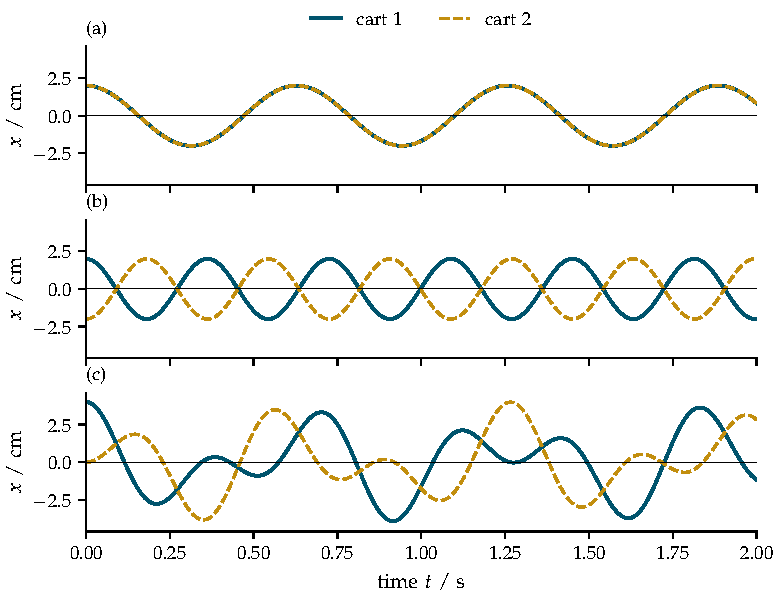
\includegraphics{ch04_oscillations/modes}
\caption{Two carts of \SI{1}{\kilogram} between walls, joined by three
springs of \SI{100}{\newton\per\metre}. (a) The slow mode: both start
\SI{2}{\centi\metre} out and swing together at
\SI{10}{\radian\per\second}. (b) The fast mode: cart
1 starts \SI{2}{\centi\metre} out one way and cart 2 \SI{2}{\centi\metre}
the other, and they swing against each other at
\SI{17.32}{\radian\per\second}. (c) Only cart 1 displaced: the sum of the
two modes, in which the swing passes back and forth between the carts.
Cart 1 is solid and cart 2 dashed, so both remain identifiable where
they move together.}
\label{fig:os-modes}
\end{figure}

\subsection*{Many atoms}

Near a minimum of the potential energy $U(\vb{r}^N)$, let $q_1, \dots,
q_n$, with $n = 3N$, be the displacements of the coordinates from the
minimum. Along the straight line from the minimum in the direction of a
displacement $\vb{q}$, the energy is $f(s) = U(\text{minimum} + s\vb{q})$.
The chain rule along a path of \cref{sec:en-gradient}, with $\dd(\text{minimum} +
s\vb{q})/\dd s = \vb{q}$, gives $f'(s) = \sum_a(\partial U/\partial
q_a)\,q_a$. Each $\partial U/\partial q_a$ is itself a function of
position, so the same rule gives its rate of change along the line as
$\sum_b(\partial^2U/\partial q_b\,\partial q_a)\,q_b$, and since the $q_a$
are fixed numbers,
\begin{equation*}
   f''(s) = \sum_a\sum_b\frac{\partial^2U}{\partial q_b\,\partial q_a}\,
   q_aq_b = \sum_{a,b}\Phi_{ab}\,q_aq_b ,
\end{equation*}
where $\sum_{a,b}$ runs over every pair $a$, $b$, $n^2$ terms in all, and
$\Phi_{ab} = \partial^2U/\partial q_a\partial q_b$, the same in either
order (\cref{sec:en-curl}), is the Hessian. At the minimum $f'(0) = 0$, so
the Taylor series of $f$ about $s = 0$, stopped after the term in $s^2$
and taken at $s = 1$, gives
\begin{equation*}
   U = U_{\min} + \tfrac12\sum_{a,b} \Phi_{ab}\,q_a q_b + \order{q^3} ,
\end{equation*}
with $\Phi_{ab}$ taken at the minimum and $q$ the length of $\vb{q}$. The
step $s = 1$ is not short, but by \cref{sec:mo-taylor} the error is at
most the largest size of $f'''$ divided by $3! = 6$, and $f'''$, from the
chain rule a third time, is a sum of third derivatives of $U$ times
products of three components of $\vb{q}$, so the error shrinks as $q^3$.
This is the many-dimensional version of \cref{sec:os-small}.

The same expansion gives the test promised in \cref{sec:en-gradient}. Let
$\vb{u}_1, \dots, \vb{u}_n$ be eigenvectors of $\boldsymbol{\Phi}$ of
length 1, at right angles to one another, with eigenvalues $\lambda_1,
\dots, \lambda_n$, and write a displacement as $\vb{q} = \sum_k
c_k\vb{u}_k$. Since $\sum_{a,b}\Phi_{ab}q_aq_b = \vb{q}\cdot
(\boldsymbol{\Phi}\vb{q})$, and $\vb{u}_k\cdot\vb{u}_l$ is 1 for $k = l$
and 0 otherwise, the quadratic term is $\frac12\sum_k\lambda_k c_k^2$.
Where the gradient vanishes, $U$ therefore has a minimum if every
eigenvalue of $\boldsymbol{\Phi}$ is positive, a maximum if every one is
negative, and a saddle point if there are some of each. Zero eigenvalues
need separate attention: higher terms may decide the behaviour, or a
symmetry may allow free motion, as in the translation below.

Differentiating the expansion with respect to $q_c$, with the other
displacements held fixed, the product rule gives each term $\Phi_{ab}q_aq_b$
the derivative $\Phi_{cb}q_b$ if $a = c$, plus $\Phi_{ac}q_a$ if $b = c$,
and nothing if neither index is $c$, so
\begin{equation*}
   \frac{\partial U}{\partial q_c}
   = \tfrac12\sum_b \Phi_{cb}\,q_b + \tfrac12\sum_a \Phi_{ac}\,q_a
   = \sum_b \Phi_{cb}\,q_b ,
\end{equation*}
the second step renaming $a$ as $b$ and using $\Phi_{bc} = \Phi_{cb}$.
Neglecting terms of order $q^2$, the force is therefore $F_c = -\sum_b
\Phi_{cb}q_b$, and Newton's law for each coordinate, $m_c\ddot{q}_c = F_c$,
reads $\vb{M}\ddot{\vb{q}} = -\boldsymbol{\Phi}\vb{q}$, with $\vb{M}$ the
diagonal matrix of the masses, each atom's mass appearing for its $x$,
$y$ and $z$. A normal mode $\vb{q} = \vb{u}\cos(\omega t + \phi)$ now needs
$\boldsymbol{\Phi}\vb{u} = \omega^2\vb{M}\vb{u}$. When the masses differ, this
is not yet an eigenvalue problem of a symmetric matrix, but the
substitution $w_a = \sqrt{m_a}\,u_a$ makes it one. The $a$th row reads
$\sum_b \Phi_{ab}u_b = \omega^2 m_a u_a$; putting $u_b = w_b/\sqrt{m_b}$
on the left and $m_au_a = \sqrt{m_a}\,w_a$ on the right, and dividing by
$\sqrt{m_a}$,
\begin{equation*}
   \sum_b \frac{\Phi_{ab}}{\sqrt{m_a m_b}}\,w_b = \omega^2 w_a ,
\end{equation*}
the eigenvalue problem of the mass-weighted Hessian, which is symmetric.
Its $n$ eigenvalues are the squared angular frequencies of the $n$ normal
modes. The function \texttt{normal\_modes} of \texttt{mdlab} solves it with
NumPy's routine for symmetric matrices, \texttt{eigh}:

\begin{code}
def normal_modes(
    hessian: ArrayLike, masses: ArrayLike, *, force_to_accel: float
) -> tuple[NDArray, NDArray]:
    hessian = np.asarray(hessian, dtype=float)
    root_m = np.sqrt(np.asarray(masses, dtype=float))
    weighted = hessian / np.outer(root_m, root_m)  # Φ_ab / √(m_a m_b)
    omega_squared, vectors = np.linalg.eigh(weighted)
    modes = vectors / root_m[:, np.newaxis]  # w_a / √m_a back to u_a
    return omega_squared * force_to_accel, modes
\end{code}

The lone \texttt{*} in the first line makes the argument after it a
keyword argument, passed by name as \texttt{force\_to\_accel=1.0}.
\texttt{np.outer(root\_m, root\_m)} is the table of products $\sqrt{m_a
m_b}$, so the division forms the mass-weighted Hessian entry by entry;
\texttt{eigh} returns its eigenvalues in increasing order and its
eigenvectors as columns, each of length 1 and of either sign.
\texttt{root\_m[:, np.newaxis]}, in which \texttt{:} takes the whole of
the one dimension that \texttt{root\_m} has, is the column of the
$\sqrt{m_a}$, as in \cref{sec:ne-atoms}, so the next division divides row
$a$ by $\sqrt{m_a}$ and turns each $\vb{w}$ back into a pattern of
displacements $\vb{u}$. The factor \texttt{force\_to\_accel} is 1 in SI
units and the Newton factor \num{9.648533e-3} of \cref{sec:ne-atoms} for a
Hessian in \si{\electronvolt\per\angstrom\squared} and masses in
\si{\amu}, giving $\omega^2$ in \si{\per\femto\second\squared}, as for
the lithium atom of \cref{sec:os-small}.

\subsection*{A linear molecule of three atoms}

A molecule like carbon dioxide, an oxygen atom on either side of a carbon
atom in a line, can be modelled along its axis by two springs of
stiffness $k$ between the three atoms, with masses $m_{\mathrm O}$,
$m_{\mathrm C}$, $m_{\mathrm O}$. Its energy is $U = \frac12 k(x_2 -
x_1)^2 + \frac12 k(x_3 - x_2)^2$, with no walls, and differentiating twice
as for the carts gives a Hessian with rows $k(1, -1, 0)$, $k(-1, 2, -1)$
and $k(0, -1, 1)$. It has three modes
(\cref{fig:os-triatomic}). The first, $\vb{u} = (1, 1, 1)$, moves the whole
molecule without stretching a spring, so $\boldsymbol{\Phi}\vb{u} =
\vb{0}$ and $\omega = 0$: no force resists this pattern, and the molecule
drifts along it at a steady velocity, a motion of the whole called a
translation. In the second, $\vb{u} = (1, 0, -1)$, the
carbon stays still while the oxygens move in and out together;
$\boldsymbol{\Phi}\vb{u} = k(1, 0, -1)$ and $\vb{M}\vb{u} = (m_{\mathrm O}, 0,
-m_{\mathrm O})$, so $\omega^2 = k/m_{\mathrm O}$. In the third, the oxygens
move one way and the carbon the other, so that the centre of mass stays
still, $m_{\mathrm O}u_1 + m_{\mathrm C}u_2 + m_{\mathrm O}u_3 = 0$ with
$u_1 = u_3 = 1$, which gives $\vb{u} = (1, -2m_{\mathrm O}/m_{\mathrm C},
1)$, and
\cref{ex:os-triatomic} shows that $\omega^2 = (k/m_{\mathrm O})(1 +
2m_{\mathrm O}/m_{\mathrm C})$. With $m_{\mathrm O} = \SI{15.999}{\amu}$ and
$m_{\mathrm C} = \SI{12.011}{\amu}$, the third mode is faster than the
second by $\sqrt{1 + 2\times15.999/12.011} = 1.914$, whatever $k$ is.

\begin{figure}[htb]
\centering
\begin{tikzpicture}[line cap=round, scale=1.0,
   disp/.style={-{Stealth[length=4pt]}, line width=0.9pt, accent}]
   \foreach \row/\name/\uo/\uc/\ut in {0/translation/0.5/0.5/0.5,
      1/symmetric stretch/0.5/0/-0.5, 2/antisymmetric stretch/0.3/-0.799/0.3} {
      \begin{scope}[yshift=-\row*1.0cm]
         \draw[black!40, line width=0.6pt] (0,0) -- (3.2,0);
         \fill[black!25, draw=black, line width=0.4pt] (0,0) circle (0.2);
         \fill[black!60, draw=black, line width=0.4pt] (1.6,0) circle (0.18);
         \fill[black!25, draw=black, line width=0.4pt] (3.2,0) circle (0.2);
         \ifdim \uo pt=0pt \else \draw[disp] (0,0.35) -- ++(\uo,0); \fi
         \ifdim \uc pt=0pt \else \draw[disp] (1.6,0.35) -- ++(\uc,0); \fi
         \ifdim \ut pt=0pt \else \draw[disp] (3.2,0.35) -- ++(\ut,0); \fi
         \node[anchor=west] at (4.2,0) {\small \name};
      \end{scope}
   }
   \node[below] at (0,-2.25) {\small O};
   \node[below] at (1.6,-2.25) {\small C};
   \node[below] at (3.2,-2.25) {\small O};
\end{tikzpicture}
\caption{The three normal modes of a linear O--C--O chain along its axis.
Arrows show the pattern $\vb{u}$ of displacements, to scale within each
mode. In the antisymmetric stretch the carbon moves $2m_{\mathrm O}/
m_{\mathrm C} = 2.66$ times as far as each oxygen, in the opposite
direction, so that the centre of mass stays still.}
\label{fig:os-triatomic}
\end{figure}

\notebook{04}{animate the normal modes of the carts and the triatomic
chain}

\begin{selfcheck}
In the slow mode of the two carts, why does the middle spring not affect
the angular frequency?
\end{selfcheck}

%=============================================================================!
% 4.10  MOLECULAR VIBRATIONS AND THE TIME STEP                                !
%=============================================================================!
\section{Molecular vibrations and the time step}
\label{sec:os-molecules}

The oscillations of this chapter are the motions of atoms in molecules.
This section turns measured vibrational frequencies into periods in
femtoseconds and draws the consequence for simulation: a computer that
advances the motion in steps must take steps short compared with the
fastest of these periods.

\subsection*{Frequencies from light}

Light is an oscillation that travels, at the speed of light $c$; its
wavelength is the distance from one crest to the next, and infrared light
has wavelengths too long for the eye to see. A molecule absorbs infrared
light at frequencies close to those of many of its normal modes, much as
a driven oscillator responds most strongly at resonance
(\cref{sec:os-driven}), and other kinds of spectrum reveal most of the
rest, so measured spectra give vibrational frequencies. Spectroscopists
quote them as wavenumbers $\tilde\nu$, the number of wavelengths of the
light per centimetre, in \si{\per\centi\metre}. In one second the light
travels a distance $c$, and so passes $c\tilde\nu$ crests, each one cycle
of the oscillation, so its frequency is $\nu = c\tilde\nu$. In the units of this book, $c =
\SI{2.99792458e8}{\metre\per\second} = \SI{2.99792458e10}{\centi\metre\per
\second} = \SI{2.99792458e-5}{\centi\metre\per\femto\second}$, the last
step dividing by $10^{15}$ femtoseconds per second, so
\begin{equation*}
   \nu = 2.99792458\times10^{-5}\,\tilde\nu ,
   \qquad
   \text{period} = \frac1\nu , \qquad \omega = 2\pi\nu ,
\end{equation*}
with $\tilde\nu$ in \si{\per\centi\metre}, $\nu$ in cycles per
femtosecond and the period in femtoseconds. In \texttt{mdlab} this speed is
\texttt{units.C\_CM\_PER\_FS}, computed from the exact SI value.

\subsection*{The fastest motions}

The vibrational frequencies of small molecules have been measured
carefully and collected in tables. \Cref{tab:os-vibrations} lists a few
from Shimanouchi's compilation\cite{Shimanouchi1972}, as given by the NIST
Chemistry WebBook\cite{NISTWebBook}, with their periods. A water molecule's
O--H stretches repeat every \SI{9}{\femto\second}, and the C--H stretches
of methane every \SI{11}{\femto\second}; the bend of water takes
\SI{21}{\femto\second}, more than twice as long as its stretches, and the
stretch of the C--C bond in ethane takes \SI{34}{\femto\second}.
Stretches of bonds to hydrogen are the fastest motions in molecules that
contain hydrogen,
for the reason found in \cref{sec:os-bodies}: the hydrogen does almost all
the moving, so the reduced mass is small and $\omega = \sqrt{k/m_{\mathrm r}}$ is
large.

\begin{table}[htb]
\centering
\caption{Measured vibrational wavenumbers of three free (gas-phase)
molecules\cite{Shimanouchi1972,NISTWebBook}, with the frequency and period
they imply.}
\label{tab:os-vibrations}
\begin{tabular}{llccc}
\toprule
molecule & motion & $\tilde\nu$ / \si{\per\centi\metre}
   & $\nu$ / \si{\per\femto\second} & period / \si{\femto\second}\\
\midrule
water & antisymmetric O--H stretch & 3756 & 0.11260 & 8.88\\
water & symmetric O--H stretch & 3657 & 0.10963 & 9.12\\
methane & C--H stretch & 3019 & 0.09051 & 11.05\\
methane & C--H stretch, all in step & 2917 & 0.08745 & 11.44\\
water & bend & 1595 & 0.04782 & 20.91\\
ethane & C--C stretch & 995 & 0.02983 & 33.52\\
\bottomrule
\end{tabular}
\end{table}

No comparably simple measured value is collected here for a lithium atom
in graphite. The model surface of \cref{sec:os-small} gives a period of
\SI{170.3}{\femto\second}, a wavenumber of \SI{196}{\per\centi\metre}, but
it was built for illustration; Chapters~16 and 17 measure the motion of
lithium in graphite with a fitted model of the forces.

\subsection*{The step of a simulation}

A computer that follows atoms advances their positions and velocities by
repeated short steps, as in \cref{sec:ne-equations}. \Cref{sec:mo-atoms}
showed that a sinusoid sampled every $\tau$ is described accurately only
when $\omega\tau$ is small, and the same holds for a motion advanced in
steps. A simulation of water must therefore take steps $\tau$ with
$\omega\tau$ small for its fastest vibration, of period
\SI{8.88}{\femto\second} and so $\omega = 2\pi/8.88 =
\SI{0.708}{\radian\per\femto\second}$: steps short compared with $1/\omega
= \SI{1.41}{\femto\second}$, even if every other motion in it is a hundred
times slower. Chapter~9 works out how much
shorter, and Chapter~11 shows how the fastest vibrations can be frozen out
so that longer steps become safe. The learned propagators planned for Part~VI take
a different route: trained on such simulations, they predict the state of
the atoms a single long step ahead.

\Needspace{9\baselineskip}
\begin{bridge}
The vibrational frequencies computed by electronic-structure codes come
from the eigenvalue problem of \cref{sec:os-modes}: the Hessian of
the Born--Oppenheimer energy, usually by finite differences of the forces,
is mass-weighted and diagonalised. The harmonic frequencies so obtained
neglect the anharmonicity of \cref{sec:os-anharmonic}, which is one
reason they differ from the measured fundamentals of
\cref{tab:os-vibrations}.
\end{bridge}

\begin{selfcheck}
A vibration has a wavenumber of \SI{1000}{\per\centi\metre}. What is its
period in femtoseconds?
\end{selfcheck}

%=============================================================================!
% 4.S  WHAT WE NOW HAVE                                                       !
%=============================================================================!
\unnumbered{What we now have}

A harmonic oscillator, $x = A\cos(\omega t + \phi)$, moves as the shadow of
a point going round a circle of radius $A$ at the angular speed $\omega$,
with its phase the starting angle on that circle. Its energy, $\frac12
kA^2$, is traded between kinetic and potential forms, which over a period
hold half each, and in the phase plane its states trace ellipses, circles
when the velocity is divided by $\omega$.

Near a smooth minimum with positive curvature, small swings are
approximately those of a spring of stiffness $U''$, which gave
the periods of a pendulum, of the bead of Chapter~3 and of a lithium atom
in a model hollow. The period of a swing of any size follows from its
energy as $2\int\dd x/v$, and in the cosine, Morse and Lennard-Jones wells
it grows with the energy, so small swings are the fastest.

A drag
proportional to the velocity makes the swing shrink by $\mathrm{e}^{-\gamma
t/2}$, or, if heavy enough, prevents any swing; a sinusoidal push gives a
steady response that peaks at resonance, with a height set by the quality
factor $\omega_0/\gamma$.

Two bodies on a spring oscillate in their
separation with the reduced mass $m_1m_2/(m_1 + m_2)$, and many coupled
bodies in the harmonic approximation move as sums of normal modes, whose patterns come from the
eigenvectors of the mass-weighted Hessian and whose squared angular
frequencies are its eigenvalues. The measured vibrations of
\cref{tab:os-vibrations} repeat every 9 to \SI{34}{\femto\second}, fastest
for bonds to hydrogen, and the fastest vibration present sets how short
the steps of a simulation must be.

Chapter~5 adds rotation, and with it the angular momentum that the forces
between atoms conserve.

%=============================================================================!
% 4.A  ANSWERS TO THE CHECKS                                                  !
%=============================================================================!
\unnumbered{Answers to the checks}
\label{sec:os-answers}

\answerto{sec:os-circle}When $\omega t + \phi = \pi/2$ the point $P$ is at the top
of the reference circle, so the block is at the centre, $x = A\cos(\pi/2)
= 0$. Its velocity is $-A\omega\sin(\pi/2) = -0.05\times10 =
\SI{-0.5}{\metre\per\second}$: it moves at its greatest speed towards
negative $x$, as $P$, at the top and going anticlockwise, moves to the
left.

\answerto{sec:os-energy}Where $U = K$, each is $E/2$, so $\frac12 kx^2 =
\frac12\times\frac12 kA^2$ and $x = \pm A/\sqrt2 = \pm4/\sqrt2 =
\pm\SI{2.83}{\centi\metre}$.

\answerto{sec:os-phase}The amplitude is $A = \sqrt{x_0^2 + (v_0/\omega)^2}
= 0.3/10 = \SI{0.03}{\metre} = \SI{3}{\centi\metre}$ by \cref{sec:ne-spring}, and the largest
speed is $A\omega = \SI{0.3}{\metre\per\second}$, so the semi-axes are
\SI{3}{\centi\metre} and \SI{0.3}{\metre\per\second}. It starts at the top
of the ellipse, $(0, \SI{0.3}{\metre\per\second})$, and moves clockwise.

\answerto{sec:os-small}The period $2\pi\sqrt{L/g}$ is proportional to
$\sqrt L$, so four times the length doubles it. The mass cancelled from
$\omega_0 = \sqrt{g/L}$, so it does not matter.

\answerto{sec:os-anharmonic}Beyond small angles the restoring force,
proportional to $\sin\theta$, grows more slowly than $\theta$, so over most
of a large swing the bob is pulled back less strongly than a spring would
pull it. At the ends of a \ang{90} swing the pull along the arc is
$mg\sin\ang{90} = mg$, against $mg\,\pi/2$ for the spring of stiffness
$mg/L$ stretched by $L\pi/2$, so the bob turns round more slowly and
spends longer there. The extra time spent near the ends outweighs the
higher speed at the bottom; \cref{eq:os-period} gives 1.180 times the
small-swing period, against 1.002 for a \ang{10} swing.

\answerto{sec:os-damped}Critical damping needs $\frac12\gamma = \omega_0$,
so $\gamma = \SI{20}{\per\second}$. With $\gamma = \SI{8}{\per\second}$,
$\omega_{\mathrm d} = \sqrt{\omega_0^2 - \frac14\gamma^2} = \sqrt{100 -
16} = \SI{9.165}{\radian\per\second}$,
and the period is $2\pi/9.165 = \SI{0.686}{\second}$.

\answerto{sec:os-driven}At $\omega = \omega_0$, $A = f/(\gamma\omega_0) =
1/(0.5\times10) = \SI{0.2}{\metre} = \SI{20}{\centi\metre}$. For a very slow push, $A \to
f/\omega_0^2 = 1/100\ \si{\metre} = \SI{1}{\centi\metre}$, the stretch of
the spring under the force held still.

\answerto{sec:os-bodies}$m_{\mathrm r} = m^2/(2m) = m/2$, and the separation
oscillates with $\omega = \sqrt{k/m_{\mathrm r}} = \sqrt{2k/m}$.

\answerto{sec:os-modes}In the slow mode both carts move by the same amount
at every instant, so the distance between them never changes and the
middle spring is never stretched: it exerts no force, and each cart swings
on its outer spring alone, with $\omega = \sqrt{k/m}$.

\answerto{sec:os-molecules}$\nu = 2.99792458\times10^{-5}\times1000 =
\SI{0.02998}{\per\femto\second}$, so the period is $1/\nu =
\SI{33.36}{\femto\second}$.

%=============================================================================!
% 4.E  EXERCISES                                                              !
%=============================================================================!
\unnumbered{Exercises}
\label{sec:os-exercises}

The exercises run from questions of understanding, through calculations,
to short derivations marked `show that'. Full solutions are in
\hyperref[sec:os-solutions]{`Solutions to the exercises'} at the end of
the book, and Notebook~04 checks every numerical answer.

\begin{exercise}[a phase of $\pi$]
\label{ex:os-phase-pi}
An oscillating block has phase $\omega t + \phi = \pi$. Where is the point
$P$ on its reference circle, where is the block, and what is it about to
do?
\end{exercise}

\begin{exercise}[a stiff spring's energy]
\label{ex:os-energy}
A block of \SI{0.2}{\kilogram} on a spring of \SI{80}{\newton\per\metre}
oscillates with an amplitude of \SI{3}{\centi\metre}. Find its energy, its
largest speed, and its speed at $x = \SI{1.5}{\centi\metre}$.
\end{exercise}

\begin{exercise}[the average of a sine squared]
\label{ex:os-average}
Show that the average of $\sin^2\omega t$ over one period is $\frac12$,
directly from $\cos 2\theta = 1 - 2\sin^2\theta$.
\end{exercise}

\begin{exercise}[a state on the ellipse]
\label{ex:os-ellipse}
The block of \cref{sec:os-circle} ($m = \SI{0.5}{\kilogram}$, $k =
\SI{50}{\newton\per\metre}$) is at $x = \SI{3}{\centi\metre}$ moving at
$v = \SI{-0.4}{\metre\per\second}$. Find its energy and the semi-axes of
its ellipse in the phase plane, and say whether $x$ is about to grow or
shrink.
\end{exercise}

\begin{exercise}[a pendulum for a clock]
\label{ex:os-clock}
How long must a pendulum be for its small swings to have a period of
\SI{2}{\second}?
\end{exercise}

\begin{exercise}[a time from the arcsine]
\label{ex:os-arcsine}
Show, from \cref{eq:os-period} and the toolbox `The derivative of an
inverse function' of \cref{sec:os-anharmonic}, that a harmonic
oscillator takes $\pi/(6\omega)$ to move from its centre to half its
amplitude, and evaluate this for $\omega = \SI{10}{\radian\per\second}$.
\end{exercise}

\begin{exercise}[the bottom of a double well]
\label{ex:os-double}
For the double well $U = U_0[(x/a)^2 - 1]^2$ of \cref{ex:en-double}, show
that small oscillations about $x = \pm a$ have $\omega_0 = \sqrt{8U_0/(m
a^2)}$.
\end{exercise}

\begin{exercise}[a round hollow]
\label{ex:os-isotropic}
On the model surface, show that along the line $x = 0$ the potential
energy is $U(0, y) = \frac14 U_{\mathrm b}[3 - 2\cos(\frac12\lvert\vb{g}
\rvert y) - \cos(\lvert\vb{g}\rvert y)]$, and that its second derivative at
the hollow, $\frac38 U_{\mathrm b}\lvert\vb{g}\rvert^2$, equals the
$2\pi^2U_{\mathrm b}/a^2$ found along $x$ in \cref{sec:os-small}.
\end{exercise}

\begin{exercise}[the steepest attraction]
\label{ex:os-lj}
At what distance is the attractive force of the Lennard-Jones well
strongest? (It is where the slope of $U_{\mathrm{LJ}}$ is greatest, so
where its second derivative is zero.)
\end{exercise}

\begin{exercise}[the curvature of the Morse well]
\label{ex:os-morse}
Show that $\dd^2 U_{\mathrm M}/\dd r^2 = 2Da^2$ at $r = r_0$ by
differentiating twice, without the series.
\end{exercise}

\begin{exercise}[a swing in a liquid]
\label{ex:os-liquid}
The block with $\omega_0 = \SI{10}{\radian\per\second}$ swings in a
liquid with $\gamma = \SI{12}{\per\second}$. Find the period of its swing
and how long its swing takes to shrink to a tenth.
\end{exercise}

\begin{exercise}[critical damping]
\label{ex:os-critical}
Show by substituting into \cref{eq:os-damped} that $x = (c_1 + c_2 t)\,
\mathrm{e}^{-\omega_0 t}$ is a motion when $\gamma = 2\omega_0$.
\end{exercise}

\begin{exercise}[off resonance]
\label{ex:os-off}
The block with $\omega_0 = \SI{10}{\radian\per\second}$, $\gamma =
\SI{2}{\per\second}$ and $f = \SI{1}{\metre\per\second\squared}$ is
pushed at $\omega = 5$ and at $\SI{15}{\radian\per\second}$. Find the
amplitude and the lag in each case.
\end{exercise}

\begin{exercise}[adding motions]
\label{ex:os-linear}
Show that if $x_1(t)$ and $x_2(t)$ are motions of the damped oscillator,
\cref{eq:os-damped}, then so is $c_1x_1 + c_2x_2$ for any numbers $c_1$
and $c_2$.
\end{exercise}

\begin{exercise}[heavy hydrogen]
\label{ex:os-isotope}
Deuterium is hydrogen with a mass of \SI{2.014}{\amu}. If an O--H bond and
an O--D bond have the same stiffness, what is the ratio of the angular
frequency of the O--D vibration to that of the O--H vibration, and by what
factor is the O--D period longer?
\end{exercise}

\begin{exercise}[a different middle spring]
\label{ex:os-coupling}
The two carts of \cref{sec:os-modes} are joined by a middle spring of
stiffness $k'$, the outer springs keeping $k$. Show that the normal modes
are still $(1, 1)$ and $(1, -1)$, with $\omega^2 = k/m$ and $(k +
2k')/m$.
\end{exercise}

\begin{exercise}[the antisymmetric stretch]
\label{ex:os-triatomic}
For the O--C--O chain of \cref{sec:os-modes}, show that $\vb{u} = (1,
-2m_{\mathrm O}/m_{\mathrm C}, 1)$ satisfies $\boldsymbol{\Phi}\vb{u} =
\omega^2\vb{M}\vb{u}$ with $\omega^2 = (k/m_{\mathrm O})(1 + 2m_{\mathrm
O}/m_{\mathrm C})$.
\end{exercise}

\begin{exercise}[a free pair]
\label{ex:os-pair}
Two masses $m_1$ and $m_2$ on a line are joined by one spring of stiffness
$k$, so that the Hessian has rows $k(1, -1)$ and $k(-1, 1)$. Show that
the mass-weighted Hessian has eigenvalues $0$ and $k/m_{\mathrm r}$, with $m_{\mathrm r}$
the reduced mass, and interpret both.
\end{exercise}

\begin{exercise}[the stiffness of an O--H bond]
\label{ex:os-stiffness}
Treating the symmetric stretch of water, \SI{3657}{\per\centi\metre}, as an
O--H bond vibrating with the reduced mass of \cref{sec:os-bodies}, find
its angular frequency in \si{\radian\per\femto\second} and the stiffness of
the bond in \si{\electronvolt\per\angstrom\squared}.
\end{exercise}

\begin{exercise}[a step of a tenth]
\label{ex:os-step}
If a simulation had to take steps no longer than a tenth of the shortest
period present, what would be the longest step for water, and how many
steps would a picosecond of simulated time take?
\end{exercise}


%=============================================================================!
% CHAPTER 5  ROTATION AND ANGULAR MOMENTUM                                    !
%=============================================================================!
\chapter{Rotation and angular momentum}
\label{ch:rotation}

%=============================================================================!
% 5.0  CHAPTER OPENING                                                        !
%=============================================================================!
Chapters~2 to 4 treated a body as a particle when its motion could be
specified by a single position. A molecule also changes its orientation
as it moves, so we now need to describe rotation and distinguish it from
motion of the centre of mass. Angular momentum supplies the corresponding
conservation law: for an isolated group with central pair forces, the
internal torques cancel and the total angular momentum stays fixed.

We begin with a puck moving in a plane, where the geometry can be followed
through its distance and angle from a fixed point. Extending that argument
to space introduces the cross product; applying it to many particles then
leads to the inertia tensor, which relates angular velocity to angular
momentum. These tools let us separate a molecule's drift and rotation
from its internal motion, and explain the count of $3N - 6$ vibrational
degrees of freedom, or $3N - 5$ for a linear molecule. Chapter~6 uses the
same distinction between allowed motions to choose coordinates for
constrained systems.

%=============================================================================!
% 5.1  TURNING IN A PLANE                                                     !
%=============================================================================!
\section{Turning in a plane}
\label{sec:ro-plane}

A puck slides without friction on a smooth level table, an air table that
floats it on a thin cushion of air. A string tied to the puck runs to a
small hole in the middle of the table and through it to a hand underneath.
Set going sideways with the string taut, the puck circles the hole; pull
the string down, and the puck circles closer and faster. This section
finds the quantity that stays fixed while the speed changes, and the
reason it does.

\subsection*{Distance and angle}

Put the origin at the hole and describe the puck's position by its
distance $r$ from the hole and the angle $\theta$ that the line from the
hole makes with the $x$ axis, so that, by the definition of sine and
cosine scaled to a circle of radius $r$ (\cref{sec:mo-trig}),
\begin{equation*}
   x = r\cos\theta , \qquad y = r\sin\theta .
\end{equation*}
These are called polar coordinates. As the puck moves, both $r$ and
$\theta$ change with time, at the rates $\dot r$ and $\dot\theta$, the dot
marking the rate of change with time as in \cref{sec:mo-acceleration}.
Differentiating $x$ and $y$ with the product rule, and $\cos\theta$ and $\sin\theta$ with the chain rule, so that
$\dd\cos\theta/\dd t = -\sin\theta\,\dot\theta$ and $\dd\sin\theta/\dd t =
\cos\theta\,\dot\theta$,
\begin{equation*}
   \dot{x} = \dot{r}\cos\theta - r\dot\theta\sin\theta , \qquad
   \dot{y} = \dot{r}\sin\theta + r\dot\theta\cos\theta .
\end{equation*}
Two vectors of length 1, called unit vectors,
make this easier to read: $\vb{e}_r = (\cos\theta, \sin\theta)$, pointing
straight away from the hole, and $\vb{e}_\theta = (-\sin\theta,
\cos\theta)$, at right angles to it in the direction of increasing
$\theta$, anticlockwise; their scalar product is $-\cos\theta\sin\theta +
\sin\theta\cos\theta = 0$. Collecting the terms in $\dot r$ and in $r\dot
\theta$ in each component, $(\dot x, \dot y) = \dot r\,(\cos\theta,
\sin\theta) + r\dot\theta\,(-\sin\theta, \cos\theta)$, so the velocity is
\begin{equation}
   \vb{v} = \dot{r}\,\vb{e}_r + r\dot\theta\,\vb{e}_\theta ,
   \label{eq:ro-polar}
\end{equation}
a part $v_r = \dot r$ straight towards or away from the hole and a part
$v_\theta = r\dot\theta$ across the line to it. On a circle $r$ is
constant, $\dot\theta$ is the angular speed $\omega$, and $v_\theta =
r\dot\theta$ is the speed $R\omega$ of \cref{sec:mo-circle}.

\subsection*{Angular momentum and torque}

For a body of mass $m$ moving in the plane, define
\begin{equation}
   L = m\,(x v_y - y v_x) ,
   \label{eq:ro-ell}
\end{equation}
its angular momentum about the origin. In polar coordinates,
\begin{align*}
   x v_y - y v_x
   &= r\cos\theta\,(\dot{r}\sin\theta + r\dot\theta\cos\theta)
      && \text{putting in $x$, $y$, $\dot x$ and $\dot y$}\\
   &\quad - r\sin\theta\,(\dot{r}\cos\theta - r\dot\theta\sin\theta)\\
   &= r^2\dot\theta\,(\cos^2\theta + \sin^2\theta) = r^2\dot\theta
      && \text{the terms in $\dot r$ cancel; $\cos^2\theta + \sin^2\theta
      = 1$,}
\end{align*}
so $L = mr^2\dot\theta = mr\,v_\theta$: the distance from the origin times
the part of the momentum across the line to it. Moving straight towards
or away from the origin gives no angular momentum; going round it
anticlockwise gives a positive $L$, clockwise a negative one. Its unit is
\si{\kilogram\metre\squared\per\second}.

How does $L$ change? Differentiating \cref{eq:ro-ell} by the product rule,
\begin{align*}
   \frac{\dd L}{\dd t}
   &= m\,(\dot{x}v_y + x\dot{v}_y - \dot{y}v_x - y\dot{v}_x)\\
   &= m\,(x a_y - y a_x)
   && \text{since $\dot x v_y = v_xv_y = \dot y v_x$ and $\dot{\vb{v}} =
      \vb{a}$,}\\
   &= x F_y - y F_x
   && \text{by the second law, $m\vb{a} = \vb{F}$.}
\end{align*}
The combination on the right is the torque of the force about the origin,
\begin{equation}
   G = x F_y - y F_x , \qquad\text{and}\qquad
   \frac{\dd L}{\dd t} = G .
   \label{eq:ro-torque-plane}
\end{equation}
Torque is to angular momentum what force is to momentum. Writing the
force as $\vb{F} = F_r\vb{e}_r + F_\theta\vb{e}_\theta$, the same algebra
as for $L$, with $F_r$ in place of $\dot r$ and $F_\theta$ in place of
$r\dot\theta$, gives $G = rF_\theta$: only the part
of the force across the line from the origin turns the body, and it turns
it more the further out it acts. Its unit is the newton metre.

This is the lever. A door turns about its hinge (\cref{fig:ro-lever}a). A
push of \SI{10}{\newton} at right angles to the door at the handle,
\SI{0.8}{\metre} from the hinge, gives a torque of $0.8\times10 =
\SI{8}{\newton\metre}$; the same torque \SI{0.2}{\metre} from the hinge
needs $8/0.2 = \SI{40}{\newton}$, and a push straight towards the hinge,
with no part across the door, does not turn it at all.

Chapter~2 noted that two equal and opposite pushes at opposite corners of
a book set it spinning although they add to zero. Put the origin at the
centre of the book, with a push $(0, F)$ at the corner $(a, b)$ and a push
$(0, -F)$ at the opposite corner $(-a, -b)$ (\cref{fig:ro-lever}b). The
net force is zero, but the torques are $aF - b\times0 = aF$ and $(-a)(-F)
- (-b)\times0 = aF$, a total of $2aF$. Such a pair of forces, adding to no
force but to a torque, is called a couple.

\begin{figure}[htb]
\centering
\begin{tikzpicture}[line cap=round, line join=round,
   force/.style={-{Stealth[length=5pt]}, line width=1.0pt, accent}]
   % (a) a door seen from above, turning about its hinge
   \begin{scope}
      \fill[black!25] (-0.15,-0.35) rectangle (0,0.35);
      \draw[line width=2.2pt, black!60] (0,0) -- (3.2,0);
      \fill (0,0) circle (0.06);
      \node[left] at (-0.2,0) {\small hinge};
      \draw[force] (2.6,0) -- (2.6,1.1) node[above] {\small $\vb{F}$};
      \draw[{Stealth[length=3pt]}-{Stealth[length=3pt]}, line width=0.4pt]
         (0,-0.45) -- (2.6,-0.45) node[midway, below] {\small $r$};
      \draw[black!50, ->, line width=0.5pt] (1.4,0.25) arc[start angle=10,
         end angle=50, radius=1.4];
      \node at (0.15,1.6) {\small (a)};
   \end{scope}
   % (b) a book pushed at two opposite corners: a couple
   \begin{scope}[xshift=6.2cm, yshift=0.2cm]
      \draw[line width=0.6pt, fill=black!8] (-1.0,-0.7) rectangle (1.0,0.7);
      \fill (0,0) circle (0.04);
      \draw[force] (1.0,0.7) -- (1.0,1.5) node[above] {\small $(0, F)$};
      \draw[force] (-1.0,-0.7) -- (-1.0,-1.5) node[below] {\small $(0, -F)$};
      \node[right] at (1.0,0.55) {\small $(a, b)$};
      \node[left] at (-1.0,-0.55) {\small $(-a, -b)$};
      \node at (-1.9,1.4) {\small (b)};
   \end{scope}
\end{tikzpicture}
\caption{Torque. (a) A door seen from above: a force $\vb{F}$ at right
angles to the door, a distance $r$ from the hinge, has the torque $rF$
about the hinge. (b) A book pushed at two opposite corners: the forces add
to zero, but their torques about the centre add to $2aF$, and the book
spins.}
\label{fig:ro-lever}
\end{figure}

\subsection*{Pulling the string}

The string pulls the puck straight towards the hole, so its force has no
part across the line to the hole, $F_\theta = 0$, and its torque about the
hole is zero. The weight of the puck and the push of the table are
vertical and turn nothing in the plane. By \cref{eq:ro-torque-plane},
therefore, $L$ does not change: the angular momentum of the puck is
conserved, whatever the hand does with the string. A force that always
points towards or away from one fixed point is called a central force,
and every central force conserves the angular momentum about its centre.

Let the puck, of mass \SI{0.2}{\kilogram}, circle at $r =
\SI{0.5}{\metre}$ with speed \SI{1.2}{\metre\per\second}, so that $L = mr
v_\theta = 0.2\times0.5\times1.2 = \SI{0.12}{\kilogram\metre\squared\per
\second}$, and pull the string down at a steady \SI{0.05}{\metre\per
\second} until $r = \SI{0.25}{\metre}$. Since $L = mrv_\theta$ stays
fixed, $v_\theta = L/(mr)$ grows as $r$ shrinks: at \SI{0.25}{\metre} the
puck goes round at $0.12/(0.2\times0.25) = \SI{2.4}{\metre\per\second}$,
twice as fast at half the distance (\cref{fig:ro-puck}). Since
$\vb{e}_r$ and $\vb{e}_\theta$ are at right angles and of length 1,
Pythagoras' theorem applied to \cref{eq:ro-polar} gives $\lvert\vb{v}
\rvert^2 = \dot r^2 + v_\theta^2$, so the kinetic energy splits into a
part across the line, $\frac12 mv_\theta^2$, and a part along it, $\frac12
m\dot r^2$. The part across the line rises from $\frac12\times0.2\times
1.2^2 = \SI{0.144}{\joule}$ to $\frac12\times0.2\times2.4^2 =
\SI{0.576}{\joule}$, while the part along the line, with $\dot r =
\SI{-0.05}{\metre\per\second}$, stays a constant $\frac12\times0.2\times
0.05^2 = \SI{0.25}{\milli\joule}$. The extra
\SI{0.432}{\joule} is the work of the hand: by \cref{sec:en-kinetic} the
change in kinetic energy is the work done on the puck, the vertical forces
do none, and the string pulls inwards while the puck moves inwards, so its
work is positive.

\begin{figure}[htb]
\centering
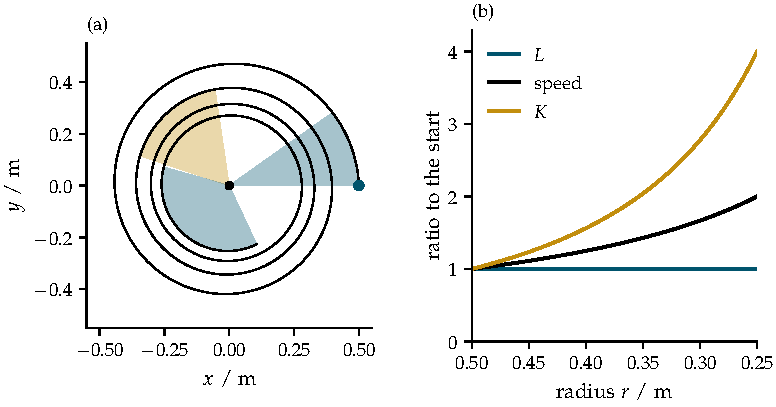
\includegraphics{ch05_rotation/puck}
\caption{A puck of \SI{0.2}{\kilogram} on a string through a hole, circling
at \SI{0.5}{\metre} and \SI{1.2}{\metre\per\second} and then pulled in at
a steady \SI{0.05}{\metre\per\second} to \SI{0.25}{\metre}, computed by
stepping Newton's second law forward in short steps of time
(\texttt{solve\_newton} in \texttt{mdlab}). (a) The path seen from above, from the dot; the
shaded sectors are swept in \SI{0.25}{\second} each, at the start, the
middle and the end of the pull, and all three have the area
\SI{0.075}{\metre\squared}. (b) The angular momentum $L$, the speed and the
kinetic energy $K$, each divided by its value at the start, against the
distance from the hole.}
\label{fig:ro-puck}
\end{figure}

\subsection*{Equal areas in equal times}

The line from the hole to the puck sweeps out area as the puck moves. A
whole circle, of area $\pi r^2$, has the angle $2\pi$, so a sector of
angle $\Delta\theta$ has the area $\pi r^2\,\Delta\theta/(2\pi) = \frac12
r^2\,\Delta\theta$. In a short time $\Delta t$ the angle grows by about
$\dot\theta\,\Delta t$, and the line sweeps a thin sector of area $\Delta A
\approx \frac12 r^2\dot\theta\,\Delta t$; the change of $r$ in that time
alters the area only by a part proportional to $(\Delta t)^2$. Dividing by
$\Delta t$ and letting $\Delta t \to 0$, as in \cref{sec:mo-velocity},
\begin{equation*}
   \frac{\dd A}{\dd t} = \tfrac12 r^2\dot\theta = \frac{L}{2m}
   \qquad\text{since $L = mr^2\dot\theta$.}
\end{equation*}
While $L$ is constant the line sweeps equal areas in equal times, here
$0.12/(2\times0.2) = \SI{0.3}{\metre\squared}$ every second: long thin
sectors far out, short wide ones close in (\cref{fig:ro-puck}a). A planet
is pulled by the Sun's gravity towards the Sun, a central force, and the
same argument gives the law of equal areas that Kepler found in the
motions of the planets.

\begin{keyidea}
In a plane, the angular momentum $L = m(xv_y - yv_x) = mr v_\theta$
changes at the rate of the torque, $G = xF_y - yF_x = rF_\theta$. A
central force has no torque about its centre, so it conserves $L$: pulled
inwards, a body goes round faster.
\end{keyidea}

\notebook{05}{pull the puck in and out and watch $L$, the speed and the
energy}

\begin{selfcheck}
The puck circling at \SI{0.5}{\metre} and \SI{1.2}{\metre\per\second} is
let out slowly to \SI{1}{\metre}. How fast does it then go round, and is
the work done on it by the string positive or negative?
\end{selfcheck}

%=============================================================================!
% 5.2  THE CROSS PRODUCT                                                      !
%=============================================================================!
\section{Angular momentum in space}
\label{sec:ro-cross}

The puck turned in the $xy$ plane, about the $z$ axis, and the combination
$xv_y - yv_x$ measured that turning. A body moving in space can turn about
any axis. Seen from far out along the $x$ axis, with the axes drawn as in
the toolbox below, the $y$ and $z$ axes sit as the $x$ and $y$ axes do
seen from above the table, so the same combination with the letters
renamed, $x \to y \to z \to x$, measures the turning about the $x$ axis,
$yv_z - zv_y$, and renaming once more gives $zv_x - xv_z$ about the $y$
axis. The three together form a vector, made from the two vectors $\vb{r}$
and $\vb{v}$ by a new product.

\begin{toolbox}[The cross product]
The cross product of $\vb{a} = (a_x, a_y, a_z)$ and $\vb{b} = (b_x, b_y,
b_z)$ is the vector
\begin{equation*}
   \vb{a}\times\vb{b} = \bigl(a_yb_z - a_zb_y,\ a_zb_x - a_xb_z,\
   a_xb_y - a_yb_x\bigr) ,
\end{equation*}
each component built from the other two letters in the order $x \to y \to
z \to x$. Its properties follow from the components:
\begin{itemize}
\item Swapping the vectors swaps the two products in every component, so
   $\vb{b}\times\vb{a} = -\vb{a}\times\vb{b}$, and $\vb{a}\times\vb{a} = \vb{0}$,
   since each of its components is a product minus the same product, such
   as $a_ya_z - a_za_y = 0$. A number factor comes outside, $(c\vb{a})\times
   \vb{b} = c\,(\vb{a}\times\vb{b})$, and a sum splits, $\vb{a}\times(\vb{b}
   + \vb{c}) = \vb{a}\times\vb{b} + \vb{a}\times\vb{c}$, since each component
   is a sum of products.
\item It is at right angles to both vectors: multiplying out,
   \begin{align*}
      \vb{a}\cdot(\vb{a}\times\vb{b})
      &= a_x(a_yb_z - a_zb_y) + a_y(a_zb_x - a_xb_z) + a_z(a_xb_y - a_yb_x)\\
      &= a_xa_yb_z - a_xa_zb_y + a_ya_zb_x - a_xa_yb_z + a_xa_zb_y - a_ya_zb_x ,
   \end{align*}
   where the first and fourth products cancel, the second and fifth, and
   the third and sixth, so the scalar product is zero; the same holds for
   $\vb{b}$, and a zero scalar product means a right angle
   (\cref{sec:mo-plane}).
\item With the unit vectors along the axes, $\vb{e}_x = (1, 0, 0)$,
   $\vb{e}_y = (0, 1, 0)$ and $\vb{e}_z = (0, 0, 1)$, the definition gives
   $\vb{e}_x\times\vb{e}_y = \vb{e}_z$, and likewise $\vb{e}_y\times\vb{e}_z
   = \vb{e}_x$ and $\vb{e}_z\times\vb{e}_x = \vb{e}_y$. We always draw the
   axes so that, curling the fingers of the right hand from $\vb{e}_x$
   towards $\vb{e}_y$, the thumb points along $\vb{e}_z$. For $\vb{a}$ and
   $\vb{b}$ in the $xy$ plane, at the angles $\theta_a$ and $\theta_b$ from the
   $x$ axis, $\vb{a}\times\vb{b} = (0, 0, a_xb_y - a_yb_x)$, and by
   \cref{eq:mo-addition} $a_xb_y - a_yb_x = \lvert\vb{a}\rvert\lvert\vb{b}
   \rvert(\cos\theta_a\sin\theta_b - \sin\theta_a\cos\theta_b) = \lvert\vb{a}\rvert
   \lvert\vb{b}\rvert\sin(\theta_b - \theta_a)$, positive when $\vb{b}$ lies
   less than half a turn anticlockwise from $\vb{a}$. So the same
   right-hand rule, fingers curling from $\vb{a}$ towards $\vb{b}$, gives
   the direction of $\vb{a}\times\vb{b}$ (\cref{fig:ro-cross}); for vectors
   in any other plane we take it on trust, since turning the axes to bring
   them into the $xy$ plane needs more than we have shown.
\item Differentiating each component by the product rule, the $x$
   component for instance as $\dd(a_yb_z - a_zb_y)/\dd t = (\dot a_yb_z -
   \dot a_zb_y) + (a_y\dot b_z - a_z\dot b_y)$, gives $\dd(\vb{a}\times
   \vb{b})/\dd t = \dot{\vb{a}}\times\vb{b} + \vb{a}\times\dot{\vb{b}}$,
   with the order of each product kept.
\end{itemize}
For example, $(1, 2, 0)\times(3, -1, 2) = (2\times2 - 0\times(-1),\
0\times3 - 1\times2,\ 1\times(-1) - 2\times3) = (4, -2, -7)$, and its
scalar products with $(1, 2, 0)$ and $(3, -1, 2)$ are $4 - 4 + 0 = 0$ and
$12 + 2 - 14 = 0$.
\end{toolbox}

\begin{toolbox}[The length of a cross product]
Squaring the three components, each by $(p - q)^2 = p^2 - 2pq + q^2$, and
adding,
\begin{align*}
   \lvert\vb{a}\times\vb{b}\rvert^2 &= a_y^2b_z^2 + a_z^2b_y^2 + a_z^2b_x^2
   + a_x^2b_z^2 + a_x^2b_y^2 + a_y^2b_x^2\\
   &\quad - 2\,(a_ya_zb_yb_z + a_za_xb_zb_x + a_xa_yb_xb_y) .
\end{align*}
The product $\lvert\vb{a}\rvert^2\lvert\vb{b}\rvert^2 = (a_x^2 + a_y^2 +
a_z^2)(b_x^2 + b_y^2 + b_z^2)$ has the same six squares plus $a_x^2b_x^2
+ a_y^2b_y^2 + a_z^2b_z^2$, and $(\vb{a}\cdot\vb{b})^2 = (a_xb_x + a_yb_y
+ a_zb_z)^2$ is those three squares plus twice the bracket above.
Subtracting,
\begin{align*}
   \lvert\vb{a}\times\vb{b}\rvert^2
   &= \lvert\vb{a}\rvert^2\lvert\vb{b}\rvert^2 - (\vb{a}\cdot\vb{b})^2\\
   &= \lvert\vb{a}\rvert^2\lvert\vb{b}\rvert^2\,(1 - \cos^2\theta)
      && \text{as $\vb{a}\cdot\vb{b} = \lvert\vb{a}\rvert\lvert\vb{b}\rvert
         \cos\theta$}\\
   &= \lvert\vb{a}\rvert^2\lvert\vb{b}\rvert^2\sin^2\theta
      && \text{as $\cos^2\theta + \sin^2\theta = 1$,}
\end{align*}
with $\theta$ the angle between the vectors, between 0 and $\pi$, by the
scalar product of \cref{sec:mo-plane}. Since $\sin\theta \ge 0$ there,
$\lvert\vb{a}\times\vb{b}\rvert = \lvert\vb{a}\rvert\lvert\vb{b}\rvert
\sin\theta$, the area of the parallelogram with sides $\vb{a}$ and
$\vb{b}$, whose base is $\lvert\vb{a}\rvert$ and height $\lvert\vb{b}\rvert
\sin\theta$. For the example above, $\lvert\vb{a}\times\vb{b}\rvert = \sqrt{4^2 + 2^2 +
7^2} = \sqrt{69} = 8.3066$, and with $\lvert\vb{a}\rvert^2 = 1 + 4 = 5$,
$\lvert\vb{b}\rvert^2 = 9 + 1 + 4 = 14$ and $\vb{a}\cdot\vb{b} = 3 - 2 + 0
= 1$, $\sqrt{5\times14 - 1^2}$ is the same.
\end{toolbox}

\begin{figure}[htb]
\centering
\begin{tikzpicture}[line cap=round, line join=round,
   vec/.style={-{Stealth[length=5pt]}, line width=1.0pt}]
   \fill[black!8] (0,0) -- (2.6,-0.5) -- (3.6,0.6) -- (1.0,1.1) -- cycle;
   \draw[vec] (0,0) -- (2.6,-0.5) node[below right] {\small $\vb{a}$};
   \draw[vec] (0,0) -- (1.0,1.1) node[above left] {\small $\vb{b}$};
   \draw[vec, accent] (0,0) -- (0,2.6) node[above]
      {\small $\vb{a}\times\vb{b}$};
   \draw[black!50, ->, line width=0.5pt] (0.9,-0.17) arc[start angle=-11,
      end angle=47, radius=0.9];
   \node at (1.1,0.32) {\small $\theta$};
   \node[black!60] at (2.45,0.52) {\small area};
   \node[black!60] at (2.45,0.2) {\small $\lvert\vb{a}\rvert
      \lvert\vb{b}\rvert\sin\theta$};
\end{tikzpicture}
\caption{The cross product, drawn in perspective: $\vb{a}$ and $\vb{b}$ lie
in a flat horizontal sheet seen from above at a slant, and $\vb{a}\times
\vb{b}$ stands straight up from it, at right angles to both, along the
thumb of a right hand whose fingers curl from $\vb{a}$ towards $\vb{b}$.
Its length is the area of the parallelogram they span (shaded).}
\label{fig:ro-cross}
\end{figure}

\subsection*{Angular momentum and torque in space}

The angular momentum about the origin of a body at $\vb{r}$ with momentum
$\vb{p} = m\vb{v}$, and the torque about the origin of a force $\vb{F}$
acting at $\vb{r}$, are
\begin{equation}
   \vb{L} = \vb{r}\times\vb{p} , \qquad \vb{G} = \vb{r}\times\vb{F} .
   \label{eq:ro-angular}
\end{equation}
By the product rule of the toolbox,
\begin{equation}
   \frac{\dd\vb{L}}{\dd t} = \vb{v}\times m\vb{v} + \vb{r}\times m\vb{a}
   = \vb{r}\times\vb{F} = \vb{G} ,
   \label{eq:ro-torque}
\end{equation}
since $\vb{v}\times\vb{v} = \vb{0}$ and $m\vb{a} = \vb{F}$: the rate of
change of the angular momentum is the torque, now as vectors. For the puck,
$\vb{r} = (x, y, 0)$ and $\vb{v} = (v_x, v_y, 0)$, so the first two
components of $\vb{L}$ vanish and $\vb{L} = (0, 0, m(xv_y - yv_x))$: the
$L$ of \cref{sec:ro-plane} is the $z$ component $L_z$ of the vector, and
$\vb{L}$ points straight up out of the table when the puck goes round
anticlockwise. In general $\lvert\vb{L}\rvert = m\lvert\vb{r}\rvert
\lvert\vb{v}\rvert\sin\theta$, with $\theta$ here the angle between
$\vb{r}$ and $\vb{v}$, as in the toolbox, not the polar angle of
\cref{sec:ro-plane}; this is the distance times the part of the
momentum at right angles to $\vb{r}$, as in the plane.

A central force, $\vb{F} = c\,\vb{r}$ for some number $c$ that may change
as the body moves (for the puck, minus the pull of the string divided by
$r$), has $\vb{G} =
c\,\vb{r}\times\vb{r} = \vb{0}$ and conserves the whole vector $\vb{L}$,
direction as well as size. Then $\vb{r}\cdot\vb{L} = m\,\vb{r}\cdot(\vb{r}
\times\vb{v}) = 0$ at every instant, by the second property in the
toolbox, so $\vb{r}$ is always at right angles to the fixed $\vb{L}$, as
the spokes of a wheel are to its axle, and a body with $\vb{L} \neq
\vb{0}$ stays in the plane through the centre at right angles to $\vb{L}$
(\cref{ex:ro-plane}). This is why a planet's orbit stays in one plane.
The puck is held in its plane by the table, but its $\vb{L}$ is fixed
too: the weight and the push of the table cancel, leaving only the
central pull of the string.

\begin{keyidea}
The cross product $\vb{a}\times\vb{b}$ is at right angles to both
vectors, by the right-hand rule, with length $\lvert\vb{a}\rvert
\lvert\vb{b}\rvert\sin\theta$. Angular momentum $\vb{L} = \vb{r}\times
\vb{p}$ changes at the rate of the torque $\vb{G} = \vb{r}\times\vb{F}$;
a central force conserves it.
\end{keyidea}

\begin{selfcheck}
Find $\vb{e}_z\times\vb{e}_x$ from the components. A record turntable
turns clockwise when seen from above. Which way does its angular momentum
point?
\end{selfcheck}

%=============================================================================!
% 5.3  THE ANGULAR MOMENTUM OF MANY BODIES                                    !
%=============================================================================!
\section{The angular momentum of many bodies}
\label{sec:ro-system}

\Cref{sec:ne-bodies} added the momenta of a group of bodies and found that
the forces between them cancel in pairs, so that only outside forces change
the total. This section does the same for angular momentum, and finds one
extra condition: the forces between two bodies must act along the line
joining them.

\subsection*{Internal torques cancel}

For $N$ bodies, at $\vb{r}_i$ with momenta $\vb{p}_i$, the total angular
momentum about the origin is
\begin{equation*}
   \vb{L} = \sum_{i=1}^{N}\vb{r}_i\times\vb{p}_i ,
\end{equation*}
and by \cref{eq:ro-torque} for each body, $\dd\vb{L}/\dd t = \sum_i\vb{r}_i
\times\vb{F}_i$, with $\vb{F}_i$ the total force on body $i$. As in
\cref{sec:ne-bodies}, split each force into the external force
$\vb{F}_i^{\mathrm{ext}}$, from outside the group, and the forces
$\vb{F}_{ij}$ on body $i$ from the other bodies $j$. The torques of the forces between bodies $i$ and $j$ appear as a
pair,
\begin{align*}
   \vb{r}_i\times\vb{F}_{ij} + \vb{r}_j\times\vb{F}_{ji}
   &= \vb{r}_i\times\vb{F}_{ij} - \vb{r}_j\times\vb{F}_{ij}
   && \text{by the third law, $\vb{F}_{ji} = -\vb{F}_{ij}$,}\\
   &= (\vb{r}_i - \vb{r}_j)\times\vb{F}_{ij}
   && \text{a sum splits, in the first vector as in the second.}
\end{align*}
The third law alone does not make this zero: two equal and opposite
forces side by side, like the pushes on the book, form a couple. But if
the force between two bodies acts along the line joining them,
$\vb{F}_{ij} = c\,(\vb{r}_i - \vb{r}_j)$ for some number $c$, the pair
gives $c\,(\vb{r}_i - \vb{r}_j)\times(\vb{r}_i - \vb{r}_j) = \vb{0}$. Then
every pair drops out, and
\begin{equation}
   \frac{\dd\vb{L}}{\dd t} = \sum_{i=1}^{N}\vb{r}_i\times
   \vb{F}_i^{\mathrm{ext}} = \vb{G}^{\mathrm{ext}} :
   \label{eq:ro-system}
\end{equation}
only the external torque changes the total angular momentum, and when it is
zero, the angular momentum of the group is conserved.

\subsection*{Forces between atoms}

Atoms whose potential energy is a sum of terms $\varphi(r_{ij})$, each
depending only on the distance $r_{ij}$ between two atoms, push and pull
along the lines joining them. Differentiating $r_{ij}^2 = (x_j - x_i)^2 +
(y_j - y_i)^2 + (z_j - z_i)^2$ with respect to $x_i$ by the chain rule
gives $2r_{ij}\,\partial r_{ij}/\partial x_i = -2(x_j - x_i)$, so
$\partial r_{ij}/\partial x_i = -(x_j - x_i)/r_{ij}$, and likewise for $y_i$
and $z_i$. The force on atom $i$ from this term is then
\begin{equation*}
   -\grad_i\varphi(r_{ij}) = -\varphi'(r_{ij})\,\grad_i r_{ij}
   = \varphi'(r_{ij})\,\frac{\vb{r}_j - \vb{r}_i}{r_{ij}} ,
\end{equation*}
along the line from atom $i$ to atom $j$, as \cref{ex:en-pair} found. An
isolated group of such atoms therefore conserves its angular momentum as
well as its momentum. Many of the forces of Chapter~8 depend on three or more atoms
at once and cannot be split into pairs, but Chapter~7 shows that, whenever
the potential energy is unchanged when the whole group is turned, the
internal torques still add to zero.

\subsection*{Turning about the centre of mass}

Unlike momentum, angular momentum depends on the point it is measured
about: about the point $\vb{a}$, each position is measured from $\vb{a}$,
so that $\sum_i(\vb{r}_i - \vb{a})\times\vb{p}_i$ takes the place of
$\vb{L}$. Measure each position and velocity from the centre of mass
$\vb{R}$ and its velocity $\vb{V} = \vb{P}/M$ (\cref{sec:ne-bodies}),
$\vb{r}_i = \vb{R} + \vb{r}_i'$ and $\vb{v}_i = \vb{V} + \vb{v}_i'$. The
primed quantities satisfy $\sum_i m_i\vb{r}_i' = \sum_i m_i\vb{r}_i -
M\vb{R} = \vb{0}$ and, differentiating, $\sum_i m_i\vb{v}_i' = \vb{0}$.
Then
\begin{align*}
   \vb{L} &= \sum_i m_i\,(\vb{R} + \vb{r}_i')\times(\vb{V} + \vb{v}_i')\\
   &= \Bigl(\sum_i m_i\Bigr)\vb{R}\times\vb{V}
      + \vb{R}\times\sum_i m_i\vb{v}_i'
      && \text{multiplying out}\\
   &\quad + \Bigl(\sum_i m_i\vb{r}_i'\Bigr)\times\vb{V}
      + \sum_i m_i\,\vb{r}_i'\times\vb{v}_i'\\
   &= \vb{R}\times\vb{P} + \vb{L}' ,
   \qquad \vb{L}' = \sum_i m_i\,\vb{r}_i'\times\vb{v}_i'
   && \text{$M\vb{V} = \vb{P}$; the middle two vanish.}
\end{align*}
The angular momentum of a group is that of its total momentum carried at
the centre of mass, plus $\vb{L}'$, its angular momentum about its own
centre of mass, which does not depend on where the origin is, since moving the origin
shifts each $\vb{r}_i$ and $\vb{R}$ alike and leaves $\vb{r}_i' = \vb{r}_i
- \vb{R}$ unchanged. For a
thrown spinning ball, the first part belongs to the flight and the second
to the spin; for a molecule, $\vb{L}'$ is the turning of the molecule
itself. For an isolated group both parts are conserved separately: $\vb{P}$
is constant, so $\dd(\vb{R}\times\vb{P})/\dd t = \vb{V}\times\vb{P} =
\vb{0}$, since $\vb{P} = M\vb{V}$ is parallel to $\vb{V}$; and $\vb{L}$ is
constant by \cref{eq:ro-system}, so $\vb{L}' = \vb{L} - \vb{R}\times\vb{P}$
is constant too.

\begin{keyidea}
Forces between pairs of bodies along the lines joining them cancel in the
total torque, so only external torques change the angular momentum of a
group, and an isolated group of atoms keeps it. The total splits into the
part carried by the centre of mass and the part $\vb{L}'$ about it.
\end{keyidea}

\begin{selfcheck}
Two bodies of \SI{1}{\kilogram} at $(\pm0.5, 0, 0)$\,\si{\metre} move with
velocities $(0, \mp1, 0)$\,\si{\metre\per\second}. Find their total
momentum and their angular momentum about the origin and about the point
$(0, 1, 0)$\,\si{\metre}.
\end{selfcheck}

%=============================================================================!
% 5.4  RIGID ROTATION                                                         !
%=============================================================================!
\section{Rigid rotation}
\label{sec:ro-rigid}

A wheel, a spinning top and, to a good approximation, a molecule are rigid:
the distances between their parts do not change as they turn. This section
finds the velocity of every part of a turning rigid body, its angular
momentum and its kinetic energy, and then keeps the promise of
\cref{sec:en-track} by racing a rolling disc and a rolling hoop against a sliding block; a
ball joins the race in \cref{ex:ro-sphere}.

\subsection*{Turning about a fixed axis}

Let a rigid body turn about the $z$ axis at the angular speed $\omega$.
Each part moves round a circle about the axis, of radius $\rho$, its
distance from the axis, at the speed $\omega\rho$ (\cref{sec:mo-circle}).
Define the angular velocity as the vector $\boldsymbol{\omega} = (0, 0,
\omega)$, along the axis, of length the angular speed, and pointing by the
right-hand rule: fingers curled along the motion, thumb along
$\boldsymbol{\omega}$. Then the velocity of the part at $\vb{r} = (x, y,
z)$ is
\begin{equation}
   \vb{v} = \boldsymbol{\omega}\times\vb{r} = (-\omega y,\ \omega x,\ 0) ,
   \label{eq:ro-rigid}
\end{equation}
by the components of the cross product; for a part at $x = \rho\cos
\omega t$, $y = \rho\sin\omega t$ this is $\rho\omega(-\sin\omega t, \cos
\omega t, 0)$, the velocity of \cref{eq:mo-circle}. For an axis
through the origin in any direction, with $\theta$ the angle between
$\boldsymbol{\omega}$ and $\vb{r}$, the length $\omega\lvert\vb{r}\rvert
\sin\theta$ of $\boldsymbol{\omega}\times\vb{r}$ is $\omega\rho$, since
$\lvert\vb{r}\rvert\sin\theta$ is the distance from the axis, and its
direction, at right angles to the axis and to $\vb{r}$ by the right-hand
rule, is along the circle the way the body turns. Neither refers to the
$x$, $y$ and $z$ axes, so $\boldsymbol{\omega}\times\vb{r}$ gives the
velocity for any such axis.

The angular momentum about the axis is the sum over the parts of
$m_i(x_iv_{y,i} - y_iv_{x,i})$, and with $v_{x,i} = -\omega y_i$ and
$v_{y,i} = \omega x_i$,
\begin{equation}
   L_z = \sum_i m_i\,\omega\,(x_i^2 + y_i^2) = I\omega , \qquad
   I = \sum_i m_i\rho_i^2 ,
   \label{eq:ro-moment}
\end{equation}
where $\rho_i^2 = x_i^2 + y_i^2$. The number $I$, the masses weighted by
their squared distances from the axis, is the moment of inertia about the
axis. The kinetic energy is likewise $\sum_i\frac12 m_i(\omega\rho_i)^2 =
\frac12 I\omega^2$. Set beside $p = mv$ and $K = \frac12 mv^2$, these say
that $I$ does for turning what the mass does for moving: the larger $I$,
the harder the body is to set turning or to stop, since a torque $G_z$
about the fixed axis changes $L_z = I\omega$ at the rate $G_z$
(\cref{eq:ro-system}), and so changes $\omega$ at the rate $G_z/I$.

\subsection*{Some moments of inertia}

\emph{Two bodies on a rod.} Masses $m_1$ and $m_2$ a distance $d$ apart
turn about an axis through their centre of mass at right angles to the
line joining them. The centre of mass is at distances $d_1$ from $m_1$
and $d_2$ from $m_2$, with $d_1 + d_2 = d$. Measured along the line from
the centre of mass, $m_1$ is at $-d_1$ and $m_2$ at $+d_2$, and by
\cref{sec:ne-bodies} $-m_1d_1 + m_2d_2 = 0$, so $m_1d_1 = m_2d_2$.
Putting $d_2 = d - d_1$ gives $(m_1 + m_2)\,d_1 = m_2d$, so $d_1 =
m_2d/(m_1 + m_2)$, and likewise $d_2 = m_1d/(m_1 + m_2)$. Then
\begin{equation}
   I = m_1d_1^2 + m_2d_2^2
   = \frac{m_1m_2^2 + m_2m_1^2}{(m_1 + m_2)^2}\,d^2
   = \frac{m_1m_2}{m_1 + m_2}\,d^2 = m_{\mathrm r}d^2 ,
   \label{eq:ro-dumbbell}
\end{equation}
since the top is $m_1m_2(m_2 + m_1)$ and one factor $m_1 + m_2$ cancels
with the bottom: the reduced mass of
\cref{sec:os-bodies} times the square of the length. A diatomic molecule
turns with this moment of inertia (\cref{sec:ro-molecules}).

\emph{A hoop} of mass $M$ and radius $R$, about its axis, has all its mass
at the distance $R$, so $I = MR^2$.

\emph{A disc} of mass $M$ and radius $R$, of even thickness, about its
axis: cut it into thin rings. The ring between $\rho$ and $\rho + \dd\rho$
has the area $2\pi\rho\,\dd\rho$, its length times its width, out of the
disc's $\pi R^2$, so its mass is $M\times2\pi\rho\,\dd\rho/(\pi R^2) =
(2M/R^2)\,\rho\,\dd\rho$, all at the distance $\rho$. Adding the rings,
\begin{equation*}
   I = \int_0^R\rho^2\,\frac{2M}{R^2}\,\rho\,\dd\rho
   = \frac{2M}{R^2}\int_0^R\rho^3\,\dd\rho
   = \frac{2M}{R^2}\Bigl[\frac{\rho^4}{4}\Bigr]_0^R
   = \frac{2M}{R^2}\,\frac{R^4}{4} = \tfrac12 MR^2 ,
\end{equation*}
taking the constant outside and integrating $\rho^3$ by
\cref{eq:mo-integrals}; half the hoop's, since much of the disc's mass lies near the axis.

\subsection*{Pulling in the arms}

A person sits on a stool that turns freely about a vertical axis, holding
a weight of \SI{2}{\kilogram} in each hand at arm's length,
\SI{0.8}{\metre} from the axis. Say that the person and the stool have
$I_0 = \SI{1.5}{\kilogram\metre\squared}$ about the axis, the same whether the arms are out or in. Then, treating
the weights as points, $I = 1.5 + 2\times2\times0.8^2 =
\SI{4.06}{\kilogram\metre\squared}$; set turning at
\SI{1}{\radian\per\second}, the stool has $L_z = \SI{4.06}{\kilogram
\metre\squared\per\second}$. Nothing outside exerts a torque about the
axis: each weight is vertical, with $F_x = F_y = 0$, so its $G_z = xF_y - yF_x$
is zero, and the bearing turns freely; by the $z$ component of
\cref{eq:ro-system}, $L_z$ is conserved. Pulling the weights in to \SI{0.2}{\metre} reduces $I$ to $1.5 +
2\times2\times0.2^2 = \SI{1.66}{\kilogram\metre\squared}$, and since $L_z
= I\omega$ is conserved, $\omega$ rises to $4.06/1.66 = \SI{2.446}{\radian
\per\second}$. The kinetic energy $\frac12 I\omega^2$ rises from
$\frac12\times4.06\times1^2 = \SI{2.030}{\joule}$ to $\frac12\times1.66
\times(4.06/1.66)^2 = \frac12\times4.06^2/1.66 = \SI{4.965}{\joule}$; the arms supply the difference,
\SI{2.935}{\joule}, by pulling the weights inwards, as the hand pulled
the puck. A spinning skater who draws in the arms speeds up for the
same reason.

\subsection*{Rolling}

\Cref{sec:en-track} let a bead slide and noted that a rolling ball also
spins, and moves more slowly. A wheel, a disc or a ball of radius $R$
rolls without slipping when the point touching the ground is momentarily
at rest. Seen from its centre, which moves at the velocity $\vb{V}$, the body
only turns, so every part has the velocity $\vb{V}$ plus the turning velocity
of \cref{eq:ro-rigid} measured from the centre, velocities adding as in
\cref{sec:ne-frames}. For a body rolling in the $+x$ direction, with $\vb{V}
= (V, 0, 0)$ and turning clockwise as seen from the $+z$ side, $x$ to the
right and $y$ up, $\boldsymbol{\omega} = (0, 0, -\omega)$,
and the bottom point, at $(0, -R, 0)$ from the centre, has the turning
velocity $(0, 0, -\omega)\times(0, -R, 0) = (-\omega R, 0, 0)$. Its total
velocity is $(V - \omega R, 0, 0)$, and rolling without slipping means
\begin{equation*}
   V = \omega R .
\end{equation*}

The kinetic energy splits like the angular momentum of
\cref{sec:ro-system}. With $\vb{v}_i = \vb{V} + \vb{v}_i'$ and $\sum_i
m_i\vb{v}_i' = \vb{0}$,
\begin{equation*}
   K = \sum_i\tfrac12 m_i\,\lvert\vb{V} + \vb{v}_i'\rvert^2
   = \tfrac12 MV^2 + \vb{V}\cdot\sum_i m_i\vb{v}_i'
     + \sum_i\tfrac12 m_i\lvert\vb{v}_i'\rvert^2
   = \tfrac12 MV^2 + \tfrac12 I\omega^2 ,
\end{equation*}
expanding the square as a scalar product; the middle term vanishes, and
the last is the energy of turning about the centre, $\frac12 I\omega^2$,
since each $\vb{v}_i'$ is the turning velocity. With $\omega = V/R$ and $I =
\kappa MR^2$, where $\kappa$ is 1 for a hoop and $\frac12$ for a disc,
\begin{equation*}
   K = \tfrac12 MV^2 + \tfrac12\kappa MR^2\,\frac{V^2}{R^2}
   = \tfrac12\,(1 + \kappa)\,MV^2 .
\end{equation*}
To roll, the body needs a grip on the ground, a friction force along the
ground at the point of contact; but that point is at rest, so the power $\vb{F}\cdot\vb{v}$ of the friction, and of the ground's push
at the same point, is zero and neither does work. The forces holding the
body together do none either: a pair $\vb{F}_{ij} = c\,(\vb{r}_i -
\vb{r}_j)$ has the power $\vb{F}_{ij}\cdot(\vb{v}_i - \vb{v}_j) = \frac12
c\,\dd\lvert\vb{r}_i - \vb{r}_j\rvert^2/\dd t$, zero since the distance is
fixed (\cref{sec:en-bodies}). Only the weight works, and a body
rolling from rest down a height $h$ has $\frac12(1 + \kappa)MV^2 = Mgh$, so
\begin{equation*}
   V = \sqrt{\frac{2gh}{1 + \kappa}} ,
\end{equation*}
whatever its mass and radius. After a drop of \SI{1}{\metre}, a block
sliding without friction ($\kappa = 0$) moves at \SI{4.429}{\metre\per
\second}, a rolling disc at \SI{3.616}{\metre\per\second} and a rolling
hoop at \SI{3.132}{\metre\per\second}: a third of the disc's kinetic
energy and half the hoop's are in the turning, $\kappa/(1 + \kappa)$. On a
slope at the angle $\alpha$, the height fallen after a distance $s$ is
$s\sin\alpha$, so $V^2 = 2gs\sin\alpha/(1 + \kappa)$; differentiating with
respect to time, by the chain rule on the left, $2V\dot{V} =
2g\sin\alpha\,\dot{s}/(1 + \kappa)$, and with $\dot s = V$, dividing both
sides by $2V$, the acceleration is the constant
\begin{equation*}
   \dot{V} = \frac{g\sin\alpha}{1 + \kappa} .
\end{equation*}
On a slope of \ang{30}, with $\sin\ang{30} = \frac12$, it is $g/2 =
4.903$, $g/3 = 3.269$ and $g/4 = \SI{2.452}{\metre\per\second\squared}$.
From rest at constant acceleration each covers $s = \frac12\dot{V}t^2$
(\cref{eq:mo-constant}), so \SI{2}{\metre} takes $t = \sqrt{2\times2/
\dot{V}}$: 0.903, 1.106 and \SI{1.277}{\second} (\cref{fig:ro-rolling}). Real wheels and balls lose a
little energy as they and the ground flex, which we neglect. The spinning
wheels of the braking car of \cref{sec:en-kinetic} carry kinetic energy of
this kind, a small part of the whole because the wheels are light
compared with the car.

\begin{figure}[htb]
\centering
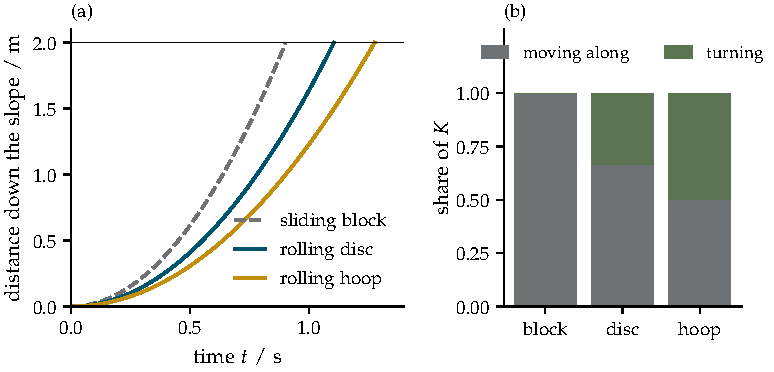
\includegraphics{ch05_rotation/rolling}
\caption{A block sliding without friction, a disc and a hoop rolling
without slipping, all released from rest on a slope of \ang{30}.
(a) Distance down the slope against time; the line marks
\SI{2}{\metre}. (b) The share of each one's kinetic energy in moving
along the slope, $\frac12 MV^2$, and in turning, $\frac12 I\omega^2$.
Neither panel depends on the mass or the radius.}
\label{fig:ro-rolling}
\end{figure}

\begin{keyidea}
A rigid body turning at $\boldsymbol{\omega}$ about a fixed axis moves
with $\vb{v} = \boldsymbol{\omega}\times\vb{r}$, and has $L_z = I\omega$
and $K = \frac12 I\omega^2$, with $I = \sum m\rho^2$. Two bodies a
distance $d$ apart have $I = m_{\mathrm r}d^2$. A rolling body keeps part
of its kinetic energy in its turning.
\end{keyidea}

\notebook{05}{race a block, a disc and a hoop down a slope}

\begin{selfcheck}
A hoop and a disc of the same mass and radius spin about their axes at the
same angular speed. Which has more kinetic energy, and by what factor?
\end{selfcheck}

%=============================================================================!
% 5.5  THE INERTIA TENSOR                                                     !
%=============================================================================!
\section{The inertia tensor}
\label{sec:ro-tensor}

\Cref{sec:ro-rigid} found the angular momentum along the axis of turning,
$L_z = I\omega$. A body can also have angular momentum across that axis:
two weights fixed to the ends of a rod, the rod clamped at a slant to an
axle, keep pulling sideways on the axle as they go round. This section
finds the whole vector $\vb{L}$ for a rigid body turning in any direction,
and with it the matrix that takes the place of the mass.

\subsection*{Angular momentum of a turning body}

Let a rigid body turn with angular velocity $\boldsymbol{\omega}$ about an
axis through its centre of mass, and measure each position $\vb{r}_i$ from
the centre of mass. Each part moves with $\vb{v}_i = \boldsymbol{\omega}
\times\vb{r}_i$, so
\begin{equation*}
   \vb{L} = \sum_i m_i\,\vb{r}_i\times(\boldsymbol{\omega}\times\vb{r}_i) .
\end{equation*}
Two rules for products of three vectors turn this into something
computable.

\begin{toolbox}[Triple products]
\emph{The vector triple product.} For any three vectors,
\begin{equation*}
   \vb{a}\times(\vb{b}\times\vb{c})
   = \vb{b}\,(\vb{a}\cdot\vb{c}) - \vb{c}\,(\vb{a}\cdot\vb{b}) .
\end{equation*}
To check the $x$ component, use $(\vb{b}\times\vb{c})_z = b_xc_y -
b_yc_x$ and $(\vb{b}\times\vb{c})_y = b_zc_x - b_xc_z$:
\begin{align*}
   \bigl[\vb{a}\times(\vb{b}\times\vb{c})\bigr]_x
   &= a_y(b_xc_y - b_yc_x) - a_z(b_zc_x - b_xc_z)\\
   &= b_x(a_yc_y + a_zc_z) - c_x(a_yb_y + a_zb_z)
   && \text{multiplying out}\\
   &= b_x(\vb{a}\cdot\vb{c}) - c_x(\vb{a}\cdot\vb{b})
   && \text{adding and subtracting $a_xb_xc_x$.}
\end{align*}
The $y$ and $z$ components follow by renaming $x \to y \to z \to x$.

\emph{The scalar triple product.} Writing out
\begin{equation*}
   \vb{a}\cdot(\vb{b}\times\vb{c})
   = a_x(b_yc_z - b_zc_y) + a_y(b_zc_x - b_xc_z) + a_z(b_xc_y - b_yc_x)
\end{equation*}
gives six products, each of one component of every vector. Writing out
\begin{equation*}
   \vb{b}\cdot(\vb{c}\times\vb{a})
   = b_x(c_ya_z - c_za_y) + b_y(c_za_x - c_xa_z) + b_z(c_xa_y - c_ya_x)
\end{equation*}
in the same way gives the same six with
the same signs, in a different order. So the three vectors may be moved
round in a cycle, $\vb{a}\cdot(\vb{b}\times\vb{c}) = \vb{b}\cdot(\vb{c}
\times\vb{a}) = \vb{c}\cdot(\vb{a}\times\vb{b})$.
\end{toolbox}

By the vector triple product with $\vb{a} = \vb{c} = \vb{r}_i$ and $\vb{b}
= \boldsymbol{\omega}$, $\vb{r}_i\times(\boldsymbol{\omega}\times\vb{r}_i)
= \boldsymbol{\omega}\,\lvert\vb{r}_i\rvert^2 - \vb{r}_i\,(\vb{r}_i\cdot
\boldsymbol{\omega})$. Its component $a$, for $a = x$, $y$ or $z$, is
$\omega_a\lvert\vb{r}_i\rvert^2 - (\vb{r}_i)_a\sum_b(\vb{r}_i)_b\omega_b$,
with $(\vb{r}_i)_a$ the component $a$ of $\vb{r}_i$. Writing $\omega_a = \sum_b\delta_{ab}
\omega_b$, where the Kronecker delta $\delta_{ab}$ is 1 when $a = b$ and 0
otherwise, so that only the term with $b = a$ survives, both terms become
sums over $b$; multiplying by $m_i$, adding over the atoms and taking the
sum over $b$ outside,
\begin{equation}
   L_a = \sum_b I_{ab}\,\omega_b , \qquad
   I_{ab} = \sum_i m_i\,\bigl(\lvert\vb{r}_i\rvert^2\delta_{ab}
   - (\vb{r}_i)_a(\vb{r}_i)_b\bigr) ,
   \label{eq:ro-tensor}
\end{equation}
or $\vb{L} = \mathsf{I}\boldsymbol{\omega}$ with the matrix product of
\cref{sec:os-modes}. The $3\times3$ matrix $\mathsf{I}$, set in sans-serif
as this book sets tensors, apart from the identity $\vb{I}$, is the
inertia tensor of the body about its centre of mass. It is symmetric,
$I_{ab} = I_{ba}$, since swapping $a$ and $b$ changes neither
$\delta_{ab}$ nor $(\vb{r}_i)_a(\vb{r}_i)_b$. Its diagonal entries are the moments of inertia about the three
axes, for instance $I_{zz} = \sum_i m_i(x_i^2 + y_i^2 + z_i^2 - z_i^2) =
\sum_i m_i(x_i^2 + y_i^2)$, as in \cref{eq:ro-moment}; its other entries,
such as $I_{xy} = -\sum_i m_ix_iy_i$, are the source of the sideways
angular momentum. For $\boldsymbol{\omega} = (0, 0, \omega)$, $\vb{L} =
\omega\,(I_{xz}, I_{yz}, I_{zz})$, along the axis only when $I_{xz}$ and
$I_{yz}$ vanish.

The kinetic energy follows with the scalar triple product. Since $\vb{v}_i
= \boldsymbol{\omega}\times\vb{r}_i$,
\begin{equation*}
   \lvert\vb{v}_i\rvert^2 = \vb{v}_i\cdot(\boldsymbol{\omega}\times\vb{r}_i)
   = \boldsymbol{\omega}\cdot(\vb{r}_i\times\vb{v}_i) ,
\end{equation*}
moving the vectors round in a cycle, so that multiplying by $\frac12 m_i$
and adding, with $\sum_i m_i\,\vb{r}_i\times\vb{v}_i = \vb{L}$,
\begin{equation}
   K = \tfrac12\,\boldsymbol{\omega}\cdot\vb{L}
   = \tfrac12\,\boldsymbol{\omega}\cdot\mathsf{I}\boldsymbol{\omega} .
   \label{eq:ro-kinetic}
\end{equation}

\subsection*{Principal axes}

Because $\mathsf{I}$ is symmetric, it has three real eigenvalues $I_1 \le
I_2 \le I_3$ with eigenvectors at right angles to one another
(\cref{sec:os-modes}). The eigenvectors are the principal axes of the
body and the eigenvalues its principal moments of inertia. Turning about
a principal axis, $\mathsf{I}\boldsymbol{\omega} = I_k\boldsymbol{\omega}$,
and the angular momentum lies along the axis; turning about any other axis,
it does not. Write $\boldsymbol{\omega} = \omega_1\vb{e}_1 + \omega_2\vb{e}_2 +
\omega_3\vb{e}_3$, with $\vb{e}_k$ the principal axes as vectors of length
1 and $\omega_k$ the parts of $\boldsymbol{\omega}$ along them. The product
is linear, so $\mathsf{I}\boldsymbol{\omega} = I_1\omega_1\vb{e}_1 +
I_2\omega_2\vb{e}_2 + I_3\omega_3\vb{e}_3$, and since $\vb{e}_j\cdot
\vb{e}_k$ is 1 for $j = k$ and 0 otherwise, \cref{eq:ro-kinetic} becomes
$K = \frac12(I_1\omega_1^2 + I_2\omega_2^2 + I_3\omega_3^2)$, as for the
quadratic term in \cref{sec:os-modes}. With the principal axes as the
coordinate axes, $\vb{e}_1 = (1, 0, 0)$ and so on, and column $k$ of the
tensor, $\mathsf{I}\vb{e}_k = I_k\vb{e}_k$, holds $I_k$ on the diagonal
and zeros elsewhere: the tensor is diagonal.

A wheel turning steadily about an axle that is not a principal axis has
an angular momentum that goes round with the wheel: worked out in axes
fixed in the wheel, with the axle as their $z$ axis, $\vb{L} =
\omega\,(I_{xz}, I_{yz}, I_{zz})$ does not change, so its sideways part
turns with the wheel. Its direction changes, so by \cref{eq:ro-system}
the bearings must supply an external torque all the time, and the axle
shakes. Car wheels are balanced by clipping small weights to
their rims until the axle passes through the centre of mass and is a
principal axis.

\subsection*{A water molecule}

The measured equilibrium geometry of water\cite{CCCBDB} has O--H bonds of
\SI{0.958}{\angstrom} at an angle of \ang{104.4776}. Place the oxygen atom
at the origin, one hydrogen atom on the $x$ axis, at $(0.958, 0, 0)$, and
the other in the $xy$ plane, at
\begin{equation*}
   (0.958\cos\ang{104.4776},\ 0.958\sin\ang{104.4776},\ 0)
   = (-0.2395, 0.9276, 0)\ \si{\angstrom}
\end{equation*}
(\cref{fig:ro-water}), with the masses 15.999 and \SI{1.008}{\amu}. The
centre of mass is at $1.008\times(0.7185, 0.9276, 0)/18.015 = (0.0402,
0.0519, 0)$\,\si{\angstrom}, and about it
\cref{eq:ro-tensor} gives, in \si{\amu\angstrom\squared},
\begin{equation*}
   \mathsf{I} = \begin{pmatrix}
      0.8188 & 0.2615 & 0\\
      0.2615 & 0.9538 & 0\\
      0 & 0 & 1.7726
   \end{pmatrix} .
\end{equation*}
The atoms lie in the plane $z = 0$, so $I_{xz} = I_{yz} = 0$ and the $z$
axis, at right angles to the molecule, is a principal axis, with $I_3 =
1.7726$. The other two come from the $2\times2$ block in the top left, by
the characteristic equation of \cref{sec:os-modes}, multiplied out with
$0.8188 + 0.9538 = 1.7726$ and $0.8188\times0.9538 - 0.2615^2 = 0.7126$:
\begin{equation*}
   (0.8188 - \lambda)(0.9538 - \lambda) - 0.2615^2
   = \lambda^2 - 1.7726\,\lambda + 0.7126 = 0 ,
\end{equation*}
so $\lambda = \frac12\bigl(1.7726 \pm\sqrt{1.7726^2 - 4\times0.7126}\bigr)
= \frac12(1.7726 \pm 0.5401)$, giving $I_1 = 0.616$ and $I_2 =
\SI{1.156}{\amu\angstrom\squared}$. The axis of $I_2$ is the line that
halves the angle between the bonds, an axis of symmetry of the molecule:
putting $\lambda = 1.1564$ into the first equation of the pair in
\cref{sec:os-modes}, $(0.8188 - 1.1564)\,u_1 + 0.2615\,u_2 = 0$, gives
$u_2/u_1 = 0.3376/0.2615 = 1.291$, a line at $\arctan1.291 = \ang{52.24}$
to the $x$ axis, half of \ang{104.4776}. The axis of $I_1$ is at right
angles to it in the plane. The two roots, $\frac12(1.7726 \pm 0.5401)$,
add to $1.7726 = 0.8188 + 0.9538 = I_{xx} + I_{yy}$, and for a flat body
$I_{xx} + I_{yy} = I_{zz}$ (\cref{ex:ro-flat}), so the largest moment, neither of the other two being negative, each a
sum of masses times squared distances, is
the sum of the other two; computed without rounding, $I_1 = 0.6162$ and
$I_2 = 1.1564$.

\begin{figure}[htb]
\centering
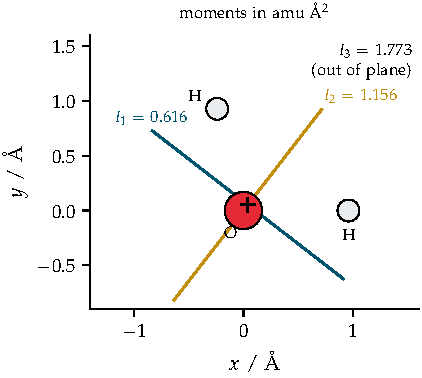
\includegraphics{ch05_rotation/water}
\caption{A water molecule at its measured geometry, one bond along $x$,
with its centre of mass (cross) and the two principal axes in its plane,
labelled with their principal moments in \si{\amu\angstrom\squared}. The
third principal axis points out of the page, with $I_3 =
\SI{1.773}{\amu\angstrom\squared}$.}
\label{fig:ro-water}
\end{figure}

A linear molecule, with every atom on one line, has a zero principal
moment about that line, since every $\rho_i$ is zero, and two equal ones
about the axes at right angles to it.

\begin{keyidea}
For a rigid body turning about its centre of mass, $\vb{L} = \mathsf{I}
\boldsymbol{\omega}$ and $K = \frac12\boldsymbol{\omega}\cdot\mathsf{I}
\boldsymbol{\omega}$, with the symmetric inertia tensor $I_{ab} = \sum_i
m_i(\lvert\vb{r}_i\rvert^2\delta_{ab} - (\vb{r}_i)_a(\vb{r}_i)_b)$. Its eigenvectors,
the principal axes, are the directions in which $\vb{L}$ is parallel to
$\boldsymbol{\omega}$.
\end{keyidea}

\notebook{05}{the inertia tensor of water and its principal axes}

\begin{selfcheck}
Two atoms of mass $m$ sit on the $z$ axis at $z = \pm d/2$. Write down
their inertia tensor about their midpoint, and its principal moments.
\end{selfcheck}

%=============================================================================!
% 5.6  REMOVING TRANSLATION AND ROTATION                                      !
%=============================================================================!
\section{Removing translation and rotation}
\label{sec:ro-remove}

A simulation of a single molecule starts from velocities chosen at random.
Their total momentum is not zero, so the molecule drifts, and their
angular momentum is not zero, so it tumbles. \Cref{sec:ne-atoms} removed
the drift by a change of frame. This section removes the tumbling too, and
shows that what remains is the motion of the atoms relative to one
another, with a kinetic energy of its own. The angular velocity of the
tumbling must be found from the angular momentum, which needs one more
tool.

\begin{toolbox}[Linear systems and the inverse matrix]
Three equations for three unknowns, such as
\begin{equation*}
   2x + y = 5 , \qquad x + 3y + z = 8 , \qquad y + 2z = 7 ,
\end{equation*}
are solved by elimination: use one equation to remove an unknown from the
others, and repeat. The first gives $x = (5 - y)/2$; putting this into the
second and multiplying by 2 gives $5 - y + 6y + 2z = 16$, or $5y + 2z =
11$; subtracting the third, $y + 2z = 7$, removes $z$ and leaves $4y = 4$,
so $y = 1$, then $z = 3$ from the third and $x = 2$ from the first. In
matrix form the equations are $\vb{A}\vb{u} = \vb{b}$, with $\vb{A}$ the
matrix of the numbers multiplying the unknowns, rows $(2, 1, 0)$, $(1, 3,
1)$ and $(0, 1, 2)$, $\vb{u} = (x, y, z)$ and $\vb{b} = (5, 8, 7)$.

When elimination gives one answer for every $\vb{b}$, the matrix has an
inverse $\vb{A}^{-1}$, the matrix that undoes it, $\vb{A}^{-1}(\vb{A}\vb{u})
= \vb{u}$, and multiplying both sides of $\vb{A}\vb{u} = \vb{b}$
by $\vb{A}^{-1}$ gives the solution $\vb{u} = \vb{A}^{-1}\vb{b}$. When
elimination instead removes a whole equation, leaving $0 = 0$ or $0 =$ a
number that is not zero, the matrix has no inverse and there are many
solutions or none. With $\vb{b} = \vb{0}$ there is always the solution
$\vb{u} = \vb{0}$, so a matrix with no inverse turns some vector $\vb{u}
\neq \vb{0}$ into $\vb{0}$. NumPy solves $\vb{A}\vb{u} = \vb{b}$ with
\texttt{np.linalg.solve}; \texttt{np.linalg.lstsq} also handles a matrix
with no inverse, returning, when there are many solutions, the shortest.
\end{toolbox}

\subsection*{The recipe}

Take the masses $m_i$, positions $\vb{r}_i$ and velocities $\vb{v}_i$ of
the atoms, and measure positions from the centre of mass, $\vb{r}_i' =
\vb{r}_i - \vb{R}$.
\begin{enumerate}
\item Subtract the velocity of the centre of mass, $\vb{V} = \vb{P}/M$,
   from every velocity: $\vb{v}_i' = \vb{v}_i - \vb{V}$.
\item Find the angular momentum about the centre of mass, $\vb{L}' =
   \sum_i m_i\vb{r}_i'\times\vb{v}_i'$, and the inertia tensor
   $\mathsf{I}$ about it, \cref{eq:ro-tensor}, and solve
   $\mathsf{I}\boldsymbol{\omega} = \vb{L}'$ for $\boldsymbol{\omega}$, the
   angular velocity of the rigid turning that carries this angular
   momentum.
\item Subtract that turning from every velocity: $\vb{u}_i = \vb{v}_i' -
   \boldsymbol{\omega}\times\vb{r}_i'$.
\end{enumerate}
The velocities $\vb{u}_i$ that remain have no total momentum and no
angular momentum. For the momentum, $\sum_i m_i\vb{u}_i = \sum_i m_i
\vb{v}_i' - \boldsymbol{\omega}\times\sum_i m_i\vb{r}_i' = \vb{0} - \vb{0}$,
by the two sums of \cref{sec:ro-system}. For the angular momentum,
\begin{equation*}
   \sum_i m_i\vb{r}_i'\times\vb{u}_i
   = \vb{L}' - \sum_i m_i\vb{r}_i'\times(\boldsymbol{\omega}\times
   \vb{r}_i') = \vb{L}' - \mathsf{I}\boldsymbol{\omega} = \vb{0} ,
\end{equation*}
by the calculation that led to \cref{eq:ro-tensor}. The inertia tensor has an inverse unless all the atoms lie on one line:
if $\mathsf{I}\vb{n} = \vb{0}$ with $\vb{n} \neq \vb{0}$, turning with
$\boldsymbol{\omega} = \vb{n}$ has, by \cref{eq:ro-kinetic},
$\sum_i\frac12 m_i\lvert\vb{n}\times\vb{r}_i'\rvert^2 =
\frac12\vb{n}\cdot\mathsf{I}\vb{n} = 0$, so every $\vb{n}\times\vb{r}_i' =
\vb{0}$ and every atom lies on the line through the centre of mass along
$\vb{n}$. For a linear molecule along the $z$ axis, $\mathsf{I}$ is
diagonal with entries $J$, $J$ and 0, where $J = \sum_i m_iz_i'^2$, and
$\vb{L}'$ has no $z$ part (every $\vb{r}_i'\times\vb{v}_i'$ is at right
angles to $\vb{r}_i'$, which lies along $z$). Then $\omega_x = L_x'/J$ and
$\omega_y = L_y'/J$, while $\omega_z$ may be anything, since turning about
the line moves no atom. We take $\omega_z = 0$, the shortest of these
solutions, which is what \texttt{lstsq} returns.

\subsection*{Three kinds of kinetic energy}

Every velocity is now a sum of three parts, $\vb{v}_i = \vb{V} +
\boldsymbol{\omega}\times\vb{r}_i' + \vb{u}_i$: the drift, the turning and
the rest. Expanding $\lvert\vb{v}_i\rvert^2 = \vb{v}_i\cdot\vb{v}_i$ term
by term,
\begin{equation*}
   \lvert\vb{v}_i\rvert^2 = V^2 + \lvert\boldsymbol{\omega}\times
   \vb{r}_i'\rvert^2 + \lvert\vb{u}_i\rvert^2
   + 2\vb{V}\cdot(\boldsymbol{\omega}\times\vb{r}_i') + 2\vb{V}\cdot
   \vb{u}_i + 2(\boldsymbol{\omega}\times\vb{r}_i')\cdot\vb{u}_i ,
\end{equation*}
and adding $\frac12 m_i$ times this over the atoms gives three squares and
three cross terms, each with $\frac12\times2 = 1$, and the cross terms all
vanish:
\begin{itemize}
\item $\sum_i m_i\vb{V}\cdot(\boldsymbol{\omega}\times\vb{r}_i') =
   \vb{V}\cdot\bigl(\boldsymbol{\omega}\times\sum_i m_i\vb{r}_i'\bigr) = 0$;
\item $\sum_i m_i\vb{V}\cdot\vb{u}_i = \vb{V}\cdot\sum_i m_i\vb{u}_i = 0$;
\item $\sum_i m_i(\boldsymbol{\omega}\times\vb{r}_i')\cdot\vb{u}_i =
   \boldsymbol{\omega}\cdot\sum_i m_i\,\vb{r}_i'\times\vb{u}_i = 0$, moving
   the vectors round in a cycle (\cref{sec:ro-tensor}).
\end{itemize}
With \cref{eq:ro-kinetic} for the turning, therefore,
\begin{equation}
   K = \tfrac12 MV^2 + \tfrac12\,\boldsymbol{\omega}\cdot\mathsf{I}
   \boldsymbol{\omega} + \sum_i\tfrac12 m_i\lvert\vb{u}_i\rvert^2 :
   \label{eq:ro-split}
\end{equation}
the kinetic energy of the drift, of the turning and of the motion of the
atoms relative to one another, each separate from the others.

\Cref{fig:ro-remove} applies the recipe to a model ring of six carbon
atoms, \SI{1.4}{\angstrom} from its centre, given velocities that drift,
turn and jostle. At the start $\vb{P} = (0.4524, 0.1738, 0)$\,\si{\amu\angstrom\per
\femto\second} and $L_z' = \SI{0.7616}{\amu\angstrom\squared\per
\femto\second}$. Removing the drift leaves $L_z'$ unchanged, since
$\sum_i m_i\vb{r}_i'\times\vb{V} = \bigl(\sum_i m_i\vb{r}_i'\bigr)\times
\vb{V} = \vb{0}$. The ring lies flat with its velocities in its plane, so,
as for water, $I_{xz} = I_{yz} = 0$ and $\vb{L}'$ points along $z$, and
$\boldsymbol{\omega} = (0, 0, L_z'/I_{zz})$. With $M = 6\times12.011 =
\SI{72.066}{\amu}$ and $I_{zz} = 6\times12.011\times1.4^2 =
\SI{141.25}{\amu\angstrom\squared}$, $\omega_z = 0.7616/141.25 =
\SI{0.00539}{\radian\per\femto\second}$, and removing that turning leaves
both at zero. The kinetic energy of \SI{0.4317}{\electronvolt} splits into
$\lvert\vb{P}\rvert^2/2M = 0.2349/(2\times72.066)\times103.6427 =
\SI{0.1689}{\electronvolt}$ of drift, $L_z'^2/2I_{zz} = 0.7616^2/(2\times
141.25)\times103.6427 = \SI{0.2128}{\electronvolt}$ of turning, and the
remaining \SI{0.0500}{\electronvolt} of motion within the ring.

\begin{figure}[htb]
\centering
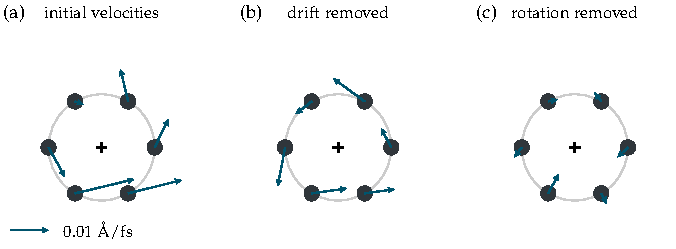
\includegraphics{ch05_rotation/remove}
\caption{A model ring of six carbon atoms with velocities in its plane
(arrows) made of a drift, a turn and a random part. (a) As made. (b)
After subtracting the velocity of the centre of mass (cross): no drift,
but the ring still turns. (c) After also subtracting the rigid turning
$\boldsymbol{\omega}\times\vb{r}'$: what remains moves the atoms relative
to one another.}
\label{fig:ro-remove}
\end{figure}

\Needspace{24\baselineskip}
\subsection*{In code}

The function \texttt{remove\_rigid\_motion} of \texttt{mdlab} follows the
recipe:

\begin{code}
def remove_rigid_motion(
    masses: ArrayLike,
    positions: ArrayLike,
    velocities: ArrayLike,
    rotation: bool = True,
) -> NDArray:
    masses = np.asarray(masses, dtype=float)
    positions = np.asarray(positions, dtype=float)
    velocities = np.asarray(velocities, dtype=float)
    total = masses.sum()
    drift = masses @ velocities / total  # V = P/M
    velocities = velocities - drift
    if rotation:
        centre = masses @ positions / total  # R
        omega = angular_velocity(masses, positions, velocities)
        velocities = velocities - np.cross(omega, positions - centre)
    return velocities
\end{code}

\texttt{masses @ velocities} is NumPy's matrix product of the list of $N$
masses with the table of velocities, $N$ rows of three: it multiplies each
row by its mass and adds the rows, giving $\sum_i m_i\vb{v}_i = \vb{P}$.
\texttt{velocities - drift} takes the three numbers of \texttt{drift}
from every row: NumPy lines up the last dimensions (\cref{sec:ne-atoms})
and repeats the shorter array down the $N$ rows, and \texttt{positions -
centre} works the same way.
\texttt{angular\_velocity} computes $\vb{L}'$ and $\mathsf{I}$ about the
centre of mass and solves for $\boldsymbol{\omega}$ with
\texttt{np.linalg.lstsq}, and \texttt{np.cross} takes the cross product of
$\boldsymbol{\omega}$ with every row of \texttt{positions - centre}. With
\texttt{rotation=False} only the drift is removed. The tests check the
result against ASE, an independent library for atomistic simulation, and
check \cref{eq:ro-split}.

\Needspace{16\baselineskip}
\begin{practice}
Most simulations follow a box of atoms repeated periodically in every
direction (Chapter~10). There the
forces still sum to zero, so the total momentum is conserved and its drift
is removed, with \texttt{rotation=False}; but turning the atoms while the box
and its copies stay fixed changes their energy, so (Chapter~7) the angular
momentum is not conserved, and
removing it would be wrong. For an isolated molecule both are removed. The
learned propagator TrajCast (discussed in the planned Chapter~28) applies the same correction to
the velocities it predicts: it adds the one velocity that restores the
total momentum to its value before the step, and, for isolated molecules,
the rigid turning $\boldsymbol{\omega}\times(\vb{r}_i - \vb{R})$ with
$\boldsymbol{\omega}$ found from the inertia tensor, at the predicted
positions, and the change in
angular momentum.
\end{practice}

\notebook{05}{switch the drift and the turning off and on, and watch the
three energies}

\begin{selfcheck}
Two atoms of \SI{1}{\amu} at $(\mp1, 0, 0)$\,\si{\angstrom} move with
velocities $(0, 0.01, 0)$ and $(0, 0.03, 0)$\,\si{\angstrom\per
\femto\second}. Find $\vb{V}$ and $\boldsymbol{\omega}$. What is left?
\end{selfcheck}

%=============================================================================!
% 5.7  DEGREES OF FREEDOM                                                     !
%=============================================================================!
\section{Degrees of freedom}
\label{sec:ro-freedom}

The positions of $N$ atoms are $3N$ numbers, so a molecule can move in
$3N$ independent ways, called its degrees of freedom. Some of these move
the molecule as a whole, without changing any distance inside it. This
section counts them, shows that they appear as zero frequencies among the
normal modes of \cref{sec:os-modes}, and finds how many ways a molecule
has left to vibrate.

\subsection*{Counting}

A rigid motion of the whole molecule is a drift in some direction, a
combination of drifts along $x$, $y$ and $z$, three ways, plus a turning
about some axis through the centre of mass, a combination of turnings
about $x$, $y$ and $z$, three more. For a linear molecule, turning about
its own line moves no atom (\cref{sec:ro-remove}), so it has only two.
What is left changes the shape of the molecule:
\begin{equation*}
   3N - 6 \text{ internal degrees of freedom, or } 3N - 5
   \text{ for a linear molecule.}
\end{equation*}
Water, with $N = 3$, has $9 - 6 = 3$, the two stretches and the bend of
\cref{tab:os-vibrations}; carbon dioxide, linear, has $9 - 5 = 4$;
methane, CH$_4$, has $15 - 6 = 9$, and benzene, C$_6$H$_6$, $36 - 6 =
30$.

\subsection*{Rigid motions as zero modes}

Near its minimum the motion of a molecule is a sum of normal modes, with
squared angular frequencies the eigenvalues of the mass-weighted Hessian
(\cref{sec:os-modes}). A rigid motion stretches nothing, so we expect
nothing to pull it back: a mode of zero frequency. We show this for a
molecule held together by springs between pairs of atoms.

\emph{The Hessian of one spring.} A spring of stiffness $k$ joins atoms $i$
and $j$ and stores $\frac12 k(r_{ij} - d)^2$, with $d$ its natural
length; we take every spring to be at its natural length at the minimum,
$r_{ij} = d$, with $\vb{e} = (\vb{r}_j - \vb{r}_i)/d$ the unit vector along
it. Displace the atoms by small amounts $\vb{q}_i$ and $\vb{q}_j$. The new
separation is $(\vb{r}_j + \vb{q}_j) - (\vb{r}_i + \vb{q}_i) = d\,\vb{e} +
\vb{q}_j - \vb{q}_i$, since $\vb{r}_j - \vb{r}_i = d\,\vb{e}$, and the new
length is its length. For a vector $\vb{a}$ and a small vector $\vb{s}$ of
length $s$, expand $\lvert\vb{a} + \vb{s}\rvert^2 = (\vb{a} + \vb{s})\cdot
(\vb{a} + \vb{s})$ and set beside it the square of a guess for the length,
chosen so that the first two terms agree:
\begin{align*}
   \lvert\vb{a} + \vb{s}\rvert^2
   &= \lvert\vb{a}\rvert^2 + 2\,\vb{a}\cdot\vb{s} + s^2 ,\\
   \Bigl(\lvert\vb{a}\rvert + \frac{\vb{a}\cdot\vb{s}}{\lvert\vb{a}\rvert}
   \Bigr)^2
   &= \lvert\vb{a}\rvert^2 + 2\,\vb{a}\cdot\vb{s}
      + \frac{(\vb{a}\cdot\vb{s})^2}{\lvert\vb{a}\rvert^2} .
\end{align*}
The two squares differ by $s^2 - (\vb{a}\cdot\vb{s})^2/\lvert\vb{a}
\rvert^2$, of order $s^2$ since $\lvert\vb{a}\cdot\vb{s}\rvert = \lvert
\vb{a}\rvert s\,\lvert\cos\theta\rvert \le \lvert\vb{a}\rvert s$, with
$\theta$ the angle between them. Two positive numbers
$X$ and $Y$ differ by $(X^2 - Y^2)/(X + Y)$, and here $X + Y$ is close to
$2\lvert\vb{a}\rvert$, so the numbers themselves differ by order $s^2$
too:
\begin{equation*}
   \lvert\vb{a} + \vb{s}\rvert = \lvert\vb{a}\rvert
   + \frac{\vb{a}\cdot\vb{s}}{\lvert\vb{a}\rvert} + \order{s^2} .
\end{equation*}
With $\vb{a} = d\,\vb{e}$ and $\vb{s} = \vb{q}_j - \vb{q}_i$, the stretch
is $r_{ij} - d = \vb{e}\cdot(\vb{q}_j - \vb{q}_i) + \order{q^2}$, with $q$
the size of the displacements. Squaring, the correction of order $q^2$
appears only multiplied by $\vb{e}\cdot(\vb{q}_j - \vb{q}_i)$, of order
$q$, or by itself, so the energy, to second order in the displacements,
is
\begin{equation*}
   U = \tfrac12 k\,\bigl[\vb{e}\cdot(\vb{q}_j - \vb{q}_i)\bigr]^2 :
\end{equation*}
only the part of the relative displacement along the spring stretches it.
By the chain rule, since $\vb{e}\cdot\vb{q}_j = \sum_b
e_b(\vb{q}_j)_b$ with $(\vb{q}_j)_b$ the component $b$ of $\vb{q}_j$, $\partial U/
\partial (\vb{q}_j)_a = ke_a\,\vb{e}\cdot(\vb{q}_j - \vb{q}_i)$ and $\partial U/
\partial (\vb{q}_i)_a = -ke_a\,\vb{e}\cdot(\vb{q}_j - \vb{q}_i)$. Differentiating
once more, $\partial^2U/\partial (\vb{q}_j)_a\partial (\vb{q}_j)_b = \partial^2U/
\partial (\vb{q}_i)_a\partial (\vb{q}_i)_b = ke_ae_b$ and $\partial^2U/\partial (\vb{q}_i)_a
\partial (\vb{q}_j)_b = -ke_ae_b$. The Hessian of the spring is made of these $3\times3$ blocks,
and that of a molecule is the sum over its springs. The function
\texttt{spring\_hessian} of \texttt{mdlab} builds it, and its tests check
it against second differences of the energy.

\emph{Rigid displacements cost no energy.} Move every atom by the same
small vector $\vb{c}$: then $\vb{q}_j - \vb{q}_i = \vb{0}$ for every
spring, and $U$ does not change. Turn the molecule through a small angle
about an axis along the unit vector $\vb{n}$ through the origin: by
\cref{eq:ro-rigid}, turning at the angular speed $\omega$ for a short time
$t$ moves each atom by its velocity times $t$, $\vb{q}_i = \omega t\,\vb{n}
\times\vb{r}_i = \theta\,\vb{n}\times\vb{r}_i$, with $\theta =
\omega t$ the small angle turned. Then
\begin{equation*}
   \vb{e}\cdot(\vb{q}_j - \vb{q}_i)
   = \theta\,\vb{e}\cdot\bigl(\vb{n}\times(\vb{r}_j - \vb{r}_i)\bigr)
   = \theta d\,\vb{e}\cdot(\vb{n}\times\vb{e}) = 0 ,
\end{equation*}
since $\vb{n}\times\vb{e}$ is at right angles to $\vb{e}$. Again no spring
is stretched. The force of a spring on atom $j$ is minus the derivative of
its energy, by the chain rule $-k\,\vb{e}\,[\vb{e}\cdot(\vb{q}_j -
\vb{q}_i)]$, and that on atom $i$ is its opposite, so for both kinds of
rigid displacement every force vanishes. The force is
$-\boldsymbol{\Phi}\vb{q}$ (\cref{sec:os-modes}), so $\boldsymbol{\Phi}
\vb{q} = \vb{0}$. With $w_b = \sqrt{m_b}\,q_b$, where $a$ and $b$ now run
over all $3N$ coordinates as in \cref{sec:os-modes}, row $a$ of the
mass-weighted Hessian gives
\begin{equation*}
   \sum_b\frac{\Phi_{ab}}{\sqrt{m_am_b}}\,\sqrt{m_b}\,q_b
   = \frac{1}{\sqrt{m_a}}\sum_b\Phi_{ab}\,q_b = 0 ,
\end{equation*}
cancelling $\sqrt{m_b}$: $\vb{w}$ is an eigenvector with eigenvalue zero, a
normal mode of zero frequency (\cref{ex:ro-null} checks a case by hand).
The three drifts and three turnings are independent, none a combination
of the others, and a symmetric matrix has as many zero eigenvalues as it
has independent vectors that it turns into zero (a general result we use
without proof, like that of \cref{sec:os-modes}), so they give six zero
modes, five for a linear molecule. The other $3N - 6$ ($3N - 5$)
eigenvalues are positive only if every change of shape costs energy, as at
the minimum of a real molecule.

The same holds for any potential energy that does not change when the
whole molecule is moved or turned, as for every isolated molecule,
provided the atoms sit at a minimum. A moved or turned copy of the minimum
is then a minimum too, where every force vanishes. A small rigid
displacement $\eta\vb{u}$ lands within $\order{\eta^2}$ of
such a copy, so the force there, $-\eta\boldsymbol{\Phi}\vb{u}$ to
first order, is of order $\eta^2$; dividing by $\eta$ and
letting $\eta$ shrink leaves $\boldsymbol{\Phi}\vb{u} = \vb{0}$.

\subsection*{A spring model of water}

Model water, at the measured geometry and with the masses of
\cref{sec:ro-tensor}, by three springs: two O--H bonds of stiffness
$k_{\mathrm{OH}}$, and an H--H spring of stiffness $k_{\mathrm{HH}}$ that
stands in for the molecule's resistance to bending; without it the bend
would cost no energy and give a seventh zero eigenvalue. Its Hessian is
$9\times9$, and with the masses of the atoms \texttt{normal\_modes} gives
nine eigenvalues. Six are zero to within the rounding error of the computer's
arithmetic, which keeps about 16 significant figures, all
below \SI{1e-15}{\per\femto\second\squared} against
\SI{0.09}{\per\femto\second\squared} for the slowest vibration: the three
drifts and the three turnings. In the antisymmetric
stretch one hydrogen atom moves out as the other moves in, and the H--H
distance does not change to first order, so $k_{\mathrm{OH}}$ alone sets
its frequency. Choosing $k_{\mathrm{OH}} = \SI{48.48}{\electronvolt\per
\angstrom\squared}$ to match the measured antisymmetric stretch of
\cref{tab:os-vibrations}, and then $k_{\mathrm{HH}} =
\SI{17.66}{\electronvolt\per\angstrom\squared}$ to match the bend, makes
the other three eigenvalues 0.09028, 0.5006 and
\SI{0.7338}{\per\femto\second\squared}; with $\omega$ the square root of
each and $\tilde\nu = \omega/(2\pi c)$ from \cref{sec:os-molecules}, they
are 1595, 3756 and \SI{4548}{\per\centi\metre}, the last, the symmetric
stretch, \SI{24}{\percent} above the measured \SI{3657}{\per\centi
\metre}. The count of modes is exact; their
frequencies are only as good as the model, and three springs are a crude
model of a molecule. A single spring between two atoms likewise gives five
zero eigenvalues and one vibration.

\Needspace{8\baselineskip}
\begin{bridge}
A vibrational analysis from electronic-structure calculations builds the
Hessian, usually by finite differences of the forces, and diagonalises its
mass-weighted form (\cref{sec:os-molecules}). The six rigid modes then come
out close to zero but not at zero: the geometry is never exactly at the
minimum, and the forces left over give the turnings a small stiffness of
either sign; the finite differences add errors of their own; and a
real-space integration grid is not quite unchanged when the atoms are
moved or turned against it. The rigid motions can then be
projected out of the Hessian before it is diagonalised, the matrix
counterpart of the recipe of \cref{sec:ro-remove}.
\end{bridge}

The count returns in Chapter~12, which measures temperature by the kinetic
energy shared among the degrees of freedom in which the atoms are free to
move. A simulation that removes the drift has three fewer, and one of an
isolated molecule that also removes the turning has six fewer, five if the
molecule is linear.

\begin{keyidea}
A molecule of $N$ atoms has $3N$ degrees of freedom: three drifts, three
turnings (two if it is linear) and $3N - 6$ ($3N - 5$) internal motions.
The rigid motions stretch nothing, and appear as zero eigenvalues of the
mass-weighted Hessian.
\end{keyidea}

\notebook{05}{the nine modes of the spring model of water}

\begin{selfcheck}
How many internal degrees of freedom has ethane, C$_2$H$_6$, and how many
has acetylene, C$_2$H$_2$, whose four atoms lie on a line?
\end{selfcheck}

%=============================================================================!
% 5.8  SPINNING MOLECULES                                                     !
%=============================================================================!
\section{Spinning molecules}
\label{sec:ro-molecules}

Molecules in a gas tumble as they fly, and the turning of a molecule is
slow compared with its vibration. This section puts numbers to that for
a molecule of lithium fluoride, LiF, one lithium atom bonded to one
fluorine atom.

\subsection*{Lithium fluoride}

The two atoms of a free LiF molecule are \SI{1.5639}{\angstrom} apart at
the bottom of their well\cite{NISTWebBook}. With the masses 6.94 and
\SI{18.998}{\amu}, the reduced mass is $6.94\times18.998/25.938 =
\SI{5.0831}{\amu}$, and by \cref{eq:ro-dumbbell} the moment of inertia
about an axis through the centre of mass at right angles to the bond is
\begin{equation*}
   I = m_{\mathrm r}d^2 = 5.0831\times1.5639^2
   = \SI{12.432}{\amu\angstrom\squared} .
\end{equation*}
We use the average mass of lithium atoms; the measured constants belong
to molecules made with the commonest, slightly heavier kind, for which $I$
is about \SI{1}{\percent} larger.
The lighter lithium atom lies $18.998/25.938\times1.5639 =
\SI{1.1455}{\angstrom}$ from the centre of mass and the fluorine atom
\SI{0.4184}{\angstrom}, so the lithium atom does most of the moving.

How fast does it turn? Chapter~12 shows that at a temperature $T$ a
freely turning molecule of two atoms carries, on average, the energy
$\kB T$ in its turning, where $\kB = \SI{8.617333e-5}{\electronvolt\per
\kelvin}$ is Boltzmann's constant; at room temperature,
\SI{300}{\kelvin} (the kelvin is the degree of the Celsius scale, counted
from \SI{-273.15}{\degreeCelsius}, so \SI{300}{\kelvin} is about
\SI{27}{\degreeCelsius}),
that is $8.617333\times10^{-5}\times300 = \SI{0.025852}{\electronvolt}$. In
the units of atoms an energy in \si{\electronvolt} becomes one in
\si{\amu\angstrom\squared\per\femto\second\squared} on multiplying by
\num{9.648533e-3} (\cref{sec:en-atoms}), and for a molecule with this average energy $K =
\frac12 I\omega^2$ gives
\begin{equation*}
   \omega = \sqrt{\frac{2K}{I}}
   = \sqrt{\frac{2\times0.025852\times9.648533\times10^{-3}}{12.432}}
   = \SI{0.006335}{\radian\per\femto\second} ,
\end{equation*}
one turn in $2\pi/\omega = \SI{992}{\femto\second}$, about a picosecond,
with the angular momentum $I\omega =
\SI{0.0788}{\amu\angstrom\squared\per\femto\second}$ along the axis of
turning (\cref{fig:ro-lif}). The lithium atom then circles at
$0.006335\times1.1455 = \SI{0.00726}{\angstrom\per\femto\second}$, or
\SI{726}{\metre\per\second}.

\begin{figure}[htb]
\centering
\begin{tikzpicture}[line cap=round, line join=round,
   vec/.style={-{Stealth[length=6pt]}, line width=1.1pt}]
   % the plane of turning, seen at a slant
   \draw[black!30, line width=0.5pt] (0,0) ellipse (2.6 and 0.75);
   \draw[black!50, ->, line width=0.6pt] (-60:2.75 and 0.88) arc[start
      angle=-60, end angle=-20, x radius=2.75, y radius=0.88];
   % the molecule: Li far from the centre, F near it
   \draw[line width=1.2pt, black!60] (-1.75,0.22) -- (0.64,-0.08);
   \shade[ball color=black!20] (-1.75,0.22) circle (0.24);
   \shade[ball color=black!45] (0.64,-0.08) circle (0.17);
   \node[above left] at (-1.85,0.38) {\small Li};
   \node[below right] at (0.72,-0.18) {\small F};
   % angular momentum along the axis
   \draw[vec, accent] (0,0) -- (0,2.0) node[above] {\small $\vb{L}$};
   \draw[black!40, dashed, line width=0.4pt] (0,0) -- (0,-1.1);
   \fill (0,0) circle (0.055);
\end{tikzpicture}
\caption{A LiF molecule turning about an axis through its centre of mass
(dot), at right angles to the bond. Its angular momentum $\vb{L} = I
\boldsymbol{\omega}$ points along the axis by the right-hand rule. The
lithium atom, the lighter, lies \SI{1.145}{\angstrom} from the centre and
the fluorine atom \SI{0.418}{\angstrom}.}
\label{fig:ro-lif}
\end{figure}

\subsection*{Fast vibration, slow turning}

The bond of LiF has the harmonic wavenumber\cite{NISTWebBook}
\SI{910.34}{\per\centi\metre}, that of small swings about the bottom of
its well, so by
\cref{sec:os-molecules} its period is
\begin{equation*}
   \frac{1}{2.99792458\times10^{-5}\times910.34}
   = \SI{36.64}{\femto\second} .
\end{equation*} The molecule therefore vibrates 27 times in each
turn, and turns only $360/27 = \ang{13}$ in each vibration. Over one
vibration it is nearly still; over one turn its length swings back and
forth 27 times about the same average, so the turning feels only that
average.
This separation of time scales is why a turning molecule is often treated
as rigid, and why the step of a simulation is set by the fastest vibrations
(\cref{sec:os-molecules}). Turning does stretch the bond a
little, since the atoms need a pull towards the centre to go round, but
for LiF at room temperature only by about \SI{0.002}{\angstrom}
(\cref{ex:ro-stretch}).

A lithium atom on the model surface of \cref{sec:en-surface} is a
different case. The surface pushes it with forces that point towards no
single centre, so in general they exert a torque about any point, and the
atom's angular momentum is not conserved. Among groups of atoms, only an isolated
one, a cluster in empty space or a molecule in a gas between collisions,
is sure to keep its angular momentum.

\notebook{05}{a turning LiF molecule with its angular momentum}

\begin{selfcheck}
At the same turning energy, how would the period of turning change for a
molecule of the same length with twice the reduced mass?
\end{selfcheck}

%=============================================================================!
% 5.S  WHAT WE NOW HAVE                                                       !
%=============================================================================!
\unnumbered{What we now have}

A body turning about a point has angular momentum $\vb{L} = \vb{r}\times
\vb{p}$, which changes at the rate of the torque $\vb{G} = \vb{r}\times
\vb{F}$; in a plane these are $L = mrv_\theta$ and $G = rF_\theta$, the
lever. A central force exerts no torque, so it conserves $\vb{L}$: a puck
pulled in on a string goes round faster, sweeping equal areas in equal
times. For a group of bodies whose forces act along the lines joining
them, as forces between atoms built from pairs do, the internal torques
cancel and only external torques change the total, which splits into a part
carried by the centre of mass and a part about it.

A rigid body turning
with angular velocity $\boldsymbol{\omega}$ moves with $\vb{v} =
\boldsymbol{\omega}\times\vb{r}$; about a fixed axis $L_z = I\omega$ and $K
= \frac12 I\omega^2$, with $I = m_{\mathrm r}d^2$ for two bodies, and a
rolling body keeps part of its energy in turning.

In general $\vb{L} =
\mathsf{I}\boldsymbol{\omega}$ and $K = \frac12\boldsymbol{\omega}\cdot
\mathsf{I}\boldsymbol{\omega}$ with the symmetric inertia tensor, whose
eigenvectors are the principal axes. Subtracting the drift $\vb{V} =
\vb{P}/M$ and the turning $\boldsymbol{\omega}\times\vb{r}'$ with
$\mathsf{I}\boldsymbol{\omega} = \vb{L}'$ removes the momentum and
the angular momentum from a set of velocities and splits the kinetic energy
into three separate parts.

The rigid motions are zero modes of the
Hessian, which leaves a molecule $3N - 6$ ways to vibrate ($3N - 5$ if it
is linear), and at room temperature a molecule such as LiF turns once in
the time it vibrates 27 times.

Chapter~6 rebuilds mechanics from the energy alone, in a form that
handles constraints, such as the rod of a pendulum, without ever finding
the forces they exert.

%=============================================================================!
% 5.A  ANSWERS TO THE CHECKS                                                  !
%=============================================================================!
\unnumbered{Answers to the checks}
\label{sec:ro-answers}

\answerto{sec:ro-plane}The string still pulls only towards the hole, so
$L = \SI{0.12}{\kilogram\metre\squared\per\second}$ is unchanged, and at
\SI{1}{\metre} the puck goes round at $v_\theta = L/(mr) = 0.12/(0.2\times1)
= \SI{0.6}{\metre\per\second}$. Its kinetic energy falls from
\SI{0.144}{\joule} to $\frac12\times0.2\times0.6^2 = \SI{0.036}{\joule}$,
so the string does the work $\SI{-0.108}{\joule}$: negative, since it
pulls inwards while the puck moves outwards.

\answerto{sec:ro-cross}By the components, $\vb{e}_z\times\vb{e}_x = (0
\times0 - 1\times0,\ 1\times1 - 0\times0,\ 0\times0 - 0\times1) = (0, 1, 0)
= \vb{e}_y$. Curling the fingers of the right hand clockwise as seen from
above, the thumb points down: the turntable's angular momentum points
straight down.

\answerto{sec:ro-system}The total momentum is $1\times(0, -1, 0) +
1\times(0, 1, 0) = \vb{0}$. About the origin, $(0.5, 0, 0)\times(0, -1, 0)
= (0, 0, -0.5)$ and $(-0.5, 0, 0)\times(0, 1, 0) = (0, 0, -0.5)$, so
$\vb{L} = (0, 0, -1)$\,\si{\kilogram\metre\squared\per\second}, a
clockwise turn seen from above. About $(0, 1, 0)$ the arms are
$(0.5, -1, 0)$ and $(-0.5, -1, 0)$, and $(0.5, -1, 0)\times(0, -1, 0) = (0,
0, -0.5)$ and $(-0.5, -1, 0)\times(0, 1, 0) = (0, 0, -0.5)$: the same
$\vb{L}$, since moving the point changes $\vb{L}$ by a term proportional to
the total momentum (\cref{ex:ro-origin}), here zero.

\answerto{sec:ro-rigid}The hoop has $K = \frac12 MR^2\omega^2$ and the disc
$\frac12\times\frac12 MR^2\omega^2$, so the hoop has twice as much: more of
its mass is far from the axis.

\answerto{sec:ro-tensor}With the atoms at $(0, 0, \pm d/2)$, $I_{xx} =
\sum m(y^2 + z^2) = 2m(d/2)^2 = \frac12 md^2$, likewise $I_{yy}$, and
$I_{zz} = \sum m(x^2 + y^2) = 0$; every product such as $-\sum mxz$ is
zero since $x = y = 0$. The tensor is diagonal, so the principal moments
are $\frac12 md^2$, $\frac12 md^2$ and 0, the first two equal to $m_{\mathrm
r}d^2$ with $m_{\mathrm r} = m/2$.

\answerto{sec:ro-remove}$\vb{V} = (0, 0.02, 0)$\,\si{\angstrom\per
\femto\second}, so $\vb{v}_1' = (0, -0.01, 0)$ and $\vb{v}_2' = (0, 0.01,
0)$. Then $\vb{L}' = (-1, 0, 0)\times(0, -0.01, 0) + (1, 0, 0)\times(0,
0.01, 0) = (0, 0, 0.02)$\,\si{\amu\angstrom\squared\per\femto\second}, and
about the centre of mass the inertia tensor is diagonal with $I_{xx} = 0$,
both atoms lying on the $x$ axis, and $I_{yy} = I_{zz} = 1\times1^2 +
1\times1^2 = \SI{2}{\amu\angstrom\squared}$. It has no inverse, so, as in
\cref{sec:ro-remove}, take $\boldsymbol{\omega}$ with no part along the
line: $\boldsymbol{\omega} = (0, 0, 0.02/2) = (0, 0,
0.01)$\,\si{\radian\per\femto\second}. The turning velocity of atom 1 is $(0, 0, 0.01)\times(-1,
0, 0) = (0, -0.01, 0) = \vb{v}_1'$, and likewise for atom 2, so nothing is
left: the pair was only drifting and turning.

\answerto{sec:ro-freedom}Ethane has 8 atoms and is not linear: $24 - 6 =
18$. Acetylene has 4 atoms on a line: $12 - 5 = 7$.

\answerto{sec:ro-molecules}With $I = m_{\mathrm r}d^2$, twice the reduced
mass doubles $I$, and at the same energy $\omega = \sqrt{2K/I}$ falls by
$\sqrt2$, so the period of turning is $\sqrt2 = 1.414$ times longer.

%=============================================================================!
% 5.E  EXERCISES                                                              !
%=============================================================================!
\unnumbered{Exercises}
\label{sec:ro-exercises}

The exercises run from questions of understanding, through calculations,
to short derivations marked `show that'. Full solutions are in
\hyperref[sec:ro-solutions]{`Solutions to the exercises'} at the end of
the book, and Notebook~05 checks every numerical answer.

\begin{exercise}[a door pushed at a slant]
\label{ex:ro-door}
Why are door handles placed far from the hinges? A push of
\SI{10}{\newton} at the handle, \SI{0.8}{\metre} from the hinge, is made at
\ang{30} to the face of the door instead of at right angles. What is its
torque about the hinge?
\end{exercise}

\begin{exercise}[pulling the puck further]
\label{ex:ro-pull}
The puck of \cref{sec:ro-plane} ($m = \SI{0.2}{\kilogram}$, circling at
\SI{0.5}{\metre} and \SI{1.2}{\metre\per\second}) is pulled in to
\SI{0.1}{\metre}. Find its speed of going round, its kinetic energy and the
work done by the hand, neglecting the slow inward motion.
\end{exercise}

\begin{exercise}[a straight line]
\label{ex:ro-straight}
Show that a body moving at constant velocity, with no force on it, has a constant
angular momentum $m\,(\vb{r} - \vb{a})\times\vb{v}$ about any point
$\vb{a}$, its position measured from $\vb{a}$, and explain, with the triangles
swept in equal times, why it sweeps equal areas in equal times.
\end{exercise}

\begin{exercise}[a cross product]
\label{ex:ro-product}
Find $(2, 0, 1)\times(1, 3, -1)$, check that it is at right angles to both
vectors, and find the area of the parallelogram they span in two ways.
\end{exercise}

\begin{exercise}[motion in a plane]
\label{ex:ro-plane}
A body moves with a constant angular momentum $\vb{L} \neq \vb{0}$ about the
origin. Show that it stays in the plane through the origin at right angles
to $\vb{L}$.
\end{exercise}

\begin{exercise}[changing the point]
\label{ex:ro-origin}
Show that the angular momentum of a group of bodies about the point
$\vb{a}$, $\sum_i(\vb{r}_i - \vb{a})\times\vb{p}_i$, equals $\vb{L} -
\vb{a}\times\vb{P}$, with $\vb{L}$ its angular momentum about the origin
and $\vb{P}$ its total momentum. When is it the same about every point?
\end{exercise}

\begin{exercise}[a rod]
\label{ex:ro-rod}
Show that a thin uniform rod of mass $M$ and length $\ell$ has the moment
of inertia $M\ell^2/12$ about an axis through its middle at right angles to
it, and $M\ell^2/3$ about a parallel axis through one end.
\end{exercise}

\begin{exercise}[the parallel axis]
\label{ex:ro-parallel}
A body has the moment of inertia $I_{\mathrm{cm}}$ about an axis through
its centre of mass. Show that about a parallel axis a distance $s$ away its
moment of inertia is $I_{\mathrm{cm}} + Ms^2$, and check the result
against \cref{ex:ro-rod}.
\end{exercise}

\begin{exercise}[the stool again]
\label{ex:ro-stool}
The stool of \cref{sec:ro-rigid}, now with $I_0 =
\SI{2}{\kilogram\metre\squared}$ and weights of \SI{3}{\kilogram} held at
\SI{0.7}{\metre}, turns at \SI{1.5}{\radian\per\second}. The weights are
pulled in to \SI{0.3}{\metre}. Find the new angular speed and the work done
by the arms.
\end{exercise}

\begin{exercise}[a rolling ball]
\label{ex:ro-sphere}
A solid ball has $I = \frac25 MR^2$ about any axis through its centre.
Rolling from rest, how fast is it moving after a drop of \SI{1}{\metre}, and
how long does it take to roll \SI{2}{\metre} down a slope of \ang{30}?
Where does it finish in the race of \cref{fig:ro-rolling}?
\end{exercise}

\begin{exercise}[the grip a disc needs]
\label{ex:ro-friction}
Using Newton's second law for the centre of mass along the slope, find the
friction force that the slope must supply to a disc of \SI{1}{\kilogram}
rolling down at \ang{30}, and show that in general it is $\kappa Mg\sin
\alpha/(1 + \kappa)$.
\end{exercise}

\begin{exercise}[a square of atoms]
\label{ex:ro-square}
Four atoms of \SI{1}{\amu} sit at $(\pm1, \pm1, 0)$\,\si{\angstrom}. Find
their inertia tensor about the origin and its principal moments. Why is
every axis through the origin in the plane of the square a principal axis?
\end{exercise}

\begin{exercise}[a flat molecule]
\label{ex:ro-flat}
Show that for a body whose parts all lie in the plane $z = 0$, $I_{zz} =
I_{xx} + I_{yy}$, and that $I_{xz} = I_{yz} = 0$, so that the $z$ axis is a
principal axis.
\end{exercise}

\begin{exercise}[a diatomic molecule]
\label{ex:ro-diatomic}
Two atoms of masses $m_1$ and $m_2$ lie on the $z$ axis a distance $d$
apart. Show that their inertia tensor about their centre of mass is
diagonal, with entries $m_{\mathrm r}d^2$, $m_{\mathrm r}d^2$ and 0.
\end{exercise}

\begin{exercise}[elimination]
\label{ex:ro-solve}
Solve, by elimination, $4\omega_x + \omega_y = 6$, $\omega_x + 4\omega_y +
\omega_z = 12$, $\omega_y + 4\omega_z = 14$.
\end{exercise}

\begin{exercise}[what is left]
\label{ex:ro-left}
Two atoms of \SI{1}{\amu} at $(\mp1, 0, 0)$\,\si{\angstrom} move with
velocities $(0.01, 0.01, 0)$ and $(-0.01, 0.03,
0)$\,\si{\angstrom\per\femto\second}. Remove the drift and the turning,
describe the motion that remains, check \cref{eq:ro-split} in
\si{\amu\angstrom\squared\per\femto\second\squared}, and give the total
kinetic energy in \si{\electronvolt}.
\end{exercise}

\begin{exercise}[counting]
\label{ex:ro-count}
How many internal degrees of freedom have ammonia, NH$_3$, and hydrogen
peroxide, H$_2$O$_2$, neither of them linear?
\end{exercise}

\begin{exercise}[a zero mode by hand]
\label{ex:ro-null}
A single spring of stiffness $k$ joins an atom at the origin to one at $(0,
0, d)$. Write down its $6\times6$ Hessian, and show directly that it turns
the displacements of a small turning about the $x$ axis into zero. Why does
a turning about the $z$ axis not count?
\end{exercise}

\begin{exercise}[a spinning bond stretches]
\label{ex:ro-stretch}
The separation of a turning LiF molecule goes round a circle, which needs a
pull $m_{\mathrm r}\omega^2 r$ towards the centre, supplied by the bond as
a spring, $k(r - d)$. Show that the bond stretches by about $d\,(\omega/
\omega_0)^2$, with $\omega_0 = \sqrt{k/m_{\mathrm r}}$
the angular frequency of the vibration, and evaluate it for the turning of
\cref{sec:ro-molecules}.
\end{exercise}

\begin{exercise}[a hotter molecule]
\label{ex:ro-hot}
At \SI{1000}{\kelvin} a LiF molecule carries on average $\kB T =
\SI{0.08617}{\electronvolt}$ in its turning. How long does one turn take?
\end{exercise}


%=============================================================================!
% CHAPTER 6  LAGRANGIAN MECHANICS                                             !
%=============================================================================!
\chapter{Lagrangian mechanics}
\label{ch:lagrange}

%=============================================================================!
% 6.0  CHAPTER OPENING                                                        !
%=============================================================================!
Newton's laws require the total force on each body, but a constraint
force is often known only through the motion it must maintain. The push
of a wire keeps a bead on its curve, and the force of a pendulum's rod
keeps the bob at a fixed distance from the pivot. Their magnitudes depend
on the motion we are trying to find. When these forces do no work, we can
instead describe the allowed motion with independent coordinates and
write the kinetic and potential energies in those coordinates.

This leads to the Lagrangian formulation of mechanics. Hamilton's
principle compares whole paths through time, and the Euler--Lagrange
equations turn that comparison into equations of motion. We apply them
to the bead on the wire of Chapter~3, then use the dependence of the
Lagrangian on its coordinates to identify conserved momenta. When the
constraint force itself is needed, a Lagrange multiplier supplies it;
Chapter~11 uses this method to hold molecular bonds at fixed lengths.
The conjugate momenta introduced here also prepare the Hamiltonian
formulation in Chapter~7.

%=============================================================================!
% 6.1  COORDINATES THAT FIT                                                   !
%=============================================================================!
\section{Coordinates that fit the problem}
\label{sec:la-coordinates}

The bead of \cref{sec:en-track} slides without friction along a wire bent
into the curve $y = h(x)$. Its position has two coordinates, $x$ and $y$,
but the wire allows only one of them to be chosen: given $x$, the bead is
at height $h(x)$. This section describes such motions by the coordinates
they actually have, and writes their energies in those coordinates.

\subsection*{The bead and the wire}

Newton's second law for the bead needs every force on it, and one of them,
the push of the wire, is unknown. It is whatever force keeps the bead on
the wire, at right angles to the wire, and its size depends on the part
of the weight across the wire as well as on how fast the bead goes and how
sharply the wire bends. \Cref{sec:en-track}
sidestepped it with energy: the push does no work, so the speed at each
height follows from $\frac12 mv^2 + mgh = E$. That gave the speed at every
point, but not directly when the bead gets there.

The energy is simplest in the one coordinate that the wire leaves free,
$x$. The bead is at $(x, h(x))$, so by the chain rule its velocity is
\begin{equation*}
   \vb{v} = \Bigl(\dot{x},\ \frac{\dd h}{\dd x}\,\dot{x}\Bigr)
   = \dot{x}\,\bigl(1,\ h'(x)\bigr) ,
\end{equation*}
the dot marking the rate of change with time (\cref{sec:mo-acceleration})
and $h'$ the slope of the wire. The square of its length, the speed
squared, is $\dot{x}^2 + h'(x)^2\dot{x}^2 = \dot{x}^2\,(1 + h'^2)$ by
Pythagoras' theorem, so
\begin{equation*}
   K = \tfrac12 m\,\bigl(1 + h'(x)^2\bigr)\,\dot{x}^2 ,
   \qquad U = mg\,h(x) .
\end{equation*}
Both energies are now written with $x$ and $\dot{x}$ alone, and the push
of the wire appears in neither.

\subsection*{The pendulum}

A pendulum's bob on a light rod of length $L$ (\cref{sec:os-small}) is
fixed by the angle $\theta$ of the rod from the vertical. With the pivot
at the origin and $y$ up, the bob is at $(L\sin\theta, -L\cos\theta)$.
Differentiating each component with the chain rule, $\dd\sin\theta/\dd t =
\cos\theta\,\dot\theta$ and $\dd\cos\theta/\dd t = -\sin\theta\,\dot\theta$
(\cref{sec:ro-plane}),
\begin{equation*}
   \vb{v} = \bigl(L\cos\theta\,\dot\theta,\ L\sin\theta\,\dot\theta\bigr)
   = L\dot\theta\,(\cos\theta, \sin\theta) ,
\end{equation*}
of length $L\lvert\dot\theta\rvert$ by Pythagoras' theorem, since
$\cos^2\theta + \sin^2\theta = 1$. The bob is $L\cos\theta$ below the
pivot, so $L - L\cos\theta$ above the bottom of the swing
(\cref{sec:os-small}), and
\begin{equation*}
   K = \tfrac12 mL^2\dot\theta^2 ,
   \qquad U = mgL\,(1 - \cos\theta) .
\end{equation*}

\subsection*{Generalised coordinates}

The fewest numbers that fix the position of every part of a system, once
its constraints are obeyed, are called its generalised coordinates; each
is free to change whatever the others do, and we write them $q_1, q_2,
\dots, q_n$. Their rates of change, $\dot{q}_1,
\dots, \dot{q}_n$, are the generalised velocities. The bead has one, $x$;
the pendulum one, $\theta$; the puck of \cref{sec:ro-plane} on its table
two, $r$ and $\theta$; and $N$ free atoms have $3N$, their Cartesian
coordinates. The number $n$ is the number of degrees of freedom of
\cref{sec:ro-freedom}. A constraint that fixes one coordinate in terms of
the others, as the wire fixes $y = h(x)$ or the rod fixes the distance
of the bob from the pivot, is called holonomic, and it removes one degree
of freedom. The wire and the rod do no work, since they push at right
angles to every motion they allow; all the constraints in this book are
holonomic and do no work.

\begin{keyidea}
Generalised coordinates are the fewest numbers that fix the position of
a system once its constraints are obeyed. In them the kinetic and potential
energies can be written without the forces of the constraints, which do
no work.
\end{keyidea}

\begin{selfcheck}
How many generalised coordinates does a double pendulum have, one bob hanging
by a rod from a second bob that hangs by a rod from a fixed pivot, moving
in a plane, and how many a rigid diatomic molecule free in space?
\end{selfcheck}

%=============================================================================!
% 6.2  THE ACTION AND HAMILTON'S PRINCIPLE                                    !
%=============================================================================!
\section{The action and Hamilton's principle}
\label{sec:la-action}

Newton's laws work forwards from a starting state, one instant to the
next. There is a second way to single out the true motion: compare whole
paths that start at one place at one time and end at another place at a
later time, and pick the one that makes a certain number stationary. This
section defines that number and tests the statement on a thrown ball;
\cref{sec:la-euler} shows that it is equivalent to Newton's laws.

\subsection*{The Lagrangian and the action}

The Lagrangian of a system is its kinetic energy minus its potential
energy,
\begin{equation}
   \Lag(q, \dot{q}) = K - U ,
   \label{eq:la-lagrangian}
\end{equation}
written, as in \cref{sec:la-coordinates}, in terms of the generalised
coordinates and velocities, $q$ standing for all of $q_1, \dots, q_n$ and
$\dot{q}$ for all of $\dot{q}_1, \dots, \dot{q}_n$. For a path $q(t)$ from the time $t_1$ to the
time $t_2$, its action is the integral
\begin{equation}
   \Act = \int_{t_1}^{t_2}\Lag\bigl(q(t), \dot{q}(t)\bigr)\,\dd t ,
   \label{eq:la-action}
\end{equation}
one number for the whole path, in joule seconds. Each path, true or not,
has an action: put its $q(t)$ and $\dot{q}(t)$ into $\Lag$ and integrate.

\emph{Hamilton's principle} states that, among all paths that start at
$q_{\mathrm{A}}$ at the time $t_1$ and end at $q_{\mathrm{B}}$ at the time
$t_2$, the path the system actually follows makes the action stationary:
changing the path from $q(t)$ to $q(t) + \zeta\eta(t)$, with $\eta$ any bump
that is zero at $t_1$ and $t_2$ and $\zeta$ a small number, changes $\Act$
by no amount proportional to $\zeta$ itself, only by amounts of order
$\zeta^2$ (\cref{sec:mo-taylor}), as at the bottom of a valley or the top
of a hill of $\Act$ against $\zeta$.

\subsection*{A thrown ball}

A ball of \SI{0.145}{\kilogram} is thrown straight up at
\SI{12}{\metre\per\second}, as in Chapters~1 to~3. Its height is $x(t) =
12t - \frac12 gt^2$ (\cref{sec:mo-integrating}), and after
\SI{2}{\second} it is \SI{4.387}{\metre} up and falling. Now invent other
paths between the same two events (an event is a place at a given time), starting at $x = 0$ at $t = 0$ and
ending at \SI{4.387}{\metre} at \SI{2}{\second}: add to the true height
$\zeta\eta(t)$, with $\eta(t) = \sin(\pi t/\tau)$ and $\tau =
\SI{2}{\second}$, a bump that is zero at both ends. Each trial path has its
own action, with $\Lag = \frac12 m\dot{x}^2 - mgx$, and the function
\texttt{action} of \texttt{mdlab} computes it by splitting the path into
short straight steps (\cref{fig:la-action}). For the true path, $\zeta =
0$, the integral can also be done by hand. With $\dot{x} = 12 - gt$,
\begin{align*}
   \Lag &= \tfrac12 m\,(12 - gt)^2 - mg\,\bigl(12t - \tfrac12 gt^2\bigr)\\
   &= 72m - 12mg\,t + \tfrac12 mg^2t^2 - 12mg\,t + \tfrac12 mg^2t^2\\
   &= 72m - 24mg\,t + mg^2t^2 ,
\end{align*}
expanding the square and the bracket, then collecting like terms,
and, integrating each term by the power rule and the fundamental theorem
(\cref{sec:mo-integrating}),
\begin{equation*}
   \Act = \Bigl[72m\,t - 12mg\,t^2 + \tfrac13 mg^2t^3\Bigr]_0^{2}
   = 20.8800 - 68.2543 + 37.1859 = \SI{-10.1884}{\joule\second} ,
\end{equation*}
as \texttt{action} also finds. The paths with $\zeta = \pm\SI{1}{\metre}$
have \SI{-10.0095}{\joule\second}, and those with $\pm\SI{2}{\metre}$ have
\SI{-9.4729}{\joule\second}. The excess grows as $\zeta^2$: \num{0.1789}
and \num{0.7155}, four times as much for twice the change, even for bumps
of metres, which are not small; the next paragraph shows why. Among these
paths the true one has the least action.

\begin{figure}[htb]
\centering
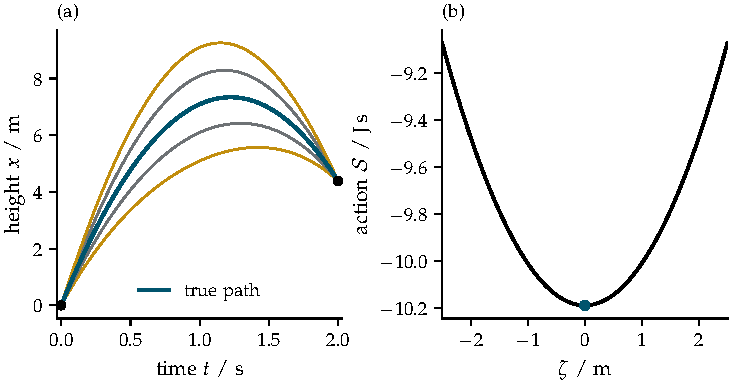
\includegraphics{ch06_lagrange/action}
\caption{Trial paths of a ball of \SI{0.145}{\kilogram} thrown up at
\SI{12}{\metre\per\second}, all starting at $x = 0$ at $t = 0$ and ending
\SI{4.387}{\metre} up at \SI{2}{\second}. (a) The true path (teal) and the
trial paths with $\zeta = \pm1$ (grey) and $\pm\SI{2}{\metre}$ (ochre).
(b) The action of each trial path against $\zeta$, least at $\zeta = 0$.}
\label{fig:la-action}
\end{figure}

The excess can be found exactly. The change of path changes the velocity
by $\zeta\dot\eta$ and the height by $\zeta\eta$, so
\begin{align*}
   \Act(\zeta) &= \int_0^\tau\Bigl[\tfrac12 m(\dot{x} + \zeta
      \dot\eta)^2 - mg\,(x + \zeta\eta)\Bigr]\dd t\\
   &= \int_0^\tau\Bigl[\bigl(\tfrac12 m\dot{x}^2 - mgx\bigr)
      + \zeta\bigl(m\dot{x}\dot\eta - mg\eta\bigr)
      + \zeta^2\,\tfrac12 m\dot\eta^2\Bigr]\dd t\\
   &= \Act(0) + \zeta\int_0^\tau\bigl(m\dot{x}\dot\eta - mg\eta\bigr)\,
      \dd t + \zeta^2\,\tfrac12 m\int_0^\tau\dot\eta^2\,\dd t ,
\end{align*}
expanding the square, grouping by powers of $\zeta$, and splitting the
integral.
There are no higher powers of $\zeta$, which is why even large bumps
follow $\zeta^2$ exactly. \Cref{sec:la-euler} shows that the middle
integral vanishes for the true path and any bump $\eta$. The last needs
$\dot\eta$ and the identity $\cos^2\theta = \frac12 + \frac12\cos2\theta$
of \cref{sec:os-energy}:
\begin{align*}
   \int_0^\tau\dot\eta^2\,\dd t
   &= \Bigl(\frac{\pi}{\tau}\Bigr)^2\int_0^\tau\cos^2\frac{\pi t}{\tau}\,
      \dd t
      && \text{$\dot\eta = \frac{\pi}{\tau}\cos\frac{\pi t}{\tau}$ by the
         chain rule,}\\
   &= \Bigl(\frac{\pi}{\tau}\Bigr)^2\int_0^\tau\Bigl(\tfrac12
      + \tfrac12\cos\frac{2\pi t}{\tau}\Bigr)\dd t
      && \text{the identity, with $\theta = \pi t/\tau$,}\\
   &= \Bigl(\frac{\pi}{\tau}\Bigr)^2\Bigl[\frac{t}{2}
      + \frac{\tau}{4\pi}\sin\frac{2\pi t}{\tau}\Bigr]_0^\tau
      && \text{the fundamental theorem,}\\
   &= \Bigl(\frac{\pi}{\tau}\Bigr)^2\frac{\tau}{2} = \frac{\pi^2}{2\tau}
      && \text{as $\sin 2\pi = \sin 0 = 0$.}
\end{align*}
The term in $\zeta^2$ is therefore $\zeta^2\times\frac12 m\times\pi^2/(2
\tau) = \zeta^2\,m\pi^2/(4\tau)$, and $m\pi^2/(4\tau) = 0.145\times9.8696/8
= \SI{0.17889}{\joule\second\per\metre\squared}$, the excess found above
for $\zeta = \SI{1}{\metre}$.

\subsection*{When the action is not least}

The true path is not always the one of least action. Take the block of
\cref{sec:os-circle}, with $m = \SI{0.5}{\kilogram}$ and $k =
\SI{50}{\newton\per\metre}$, so that $\omega = \sqrt{k/m} =
\SI{10}{\radian\per\second}$, oscillating for $\tau = \SI{0.5}{\second}$,
longer than half its period, $\pi/\omega = \SI{0.3142}{\second}$. Now
$\Lag = \frac12 m\dot{x}^2 - \frac12 kx^2$, and the potential energy of the
changed path, $\frac12 k(x + \zeta\eta)^2 = \frac12 kx^2 + \zeta kx\eta +
\zeta^2\,\frac12 k\eta^2$, brings a second term in $\zeta^2$. The term in
$\zeta$ again vanishes for the true path (\cref{sec:la-euler}), whatever
its amplitude, so for $\eta = \sin(\pi t/\tau)$ the excess is
\begin{align*}
   \Act(\zeta) - \Act(0)
   &= \zeta^2\Bigl(\tfrac12 m\int_0^\tau\dot\eta^2\,\dd t
      - \tfrac12 k\int_0^\tau\eta^2\,\dd t\Bigr)
      && \text{expanding as for the ball,}\\
   &= \zeta^2\Bigl(\tfrac12 m\Bigl(\frac{\pi}{\tau}\Bigr)^2\frac{\tau}{2}
      - \tfrac12 k\,\frac{\tau}{2}\Bigr)
      && \text{as above, with $\sin^2\theta = \tfrac12 - \tfrac12\cos2\theta$,}\\
   &= \zeta^2\,\frac{\tau}{4}\Bigl(m\Bigl(\frac{\pi}{\tau}\Bigr)^2 - k\Bigr)
      && \text{taking out $\tau/4$.}
\end{align*}
The bracket is negative whenever $\pi/\tau < \sqrt{k/m} = \omega$, that is
whenever $\tau$ is longer than $\pi/\omega$: here it is $0.125\times(0.5
\times39.48 - 50)\,\zeta^2 = -3.783\,\zeta^2$, and the action falls. For the
faster bump $\sin(2\pi t/\tau)$ the same steps with $2\pi$ in place of $\pi$
give $0.125\times(0.5\times157.91 - 50)\,\zeta^2 = +3.620\,\zeta^2$, and the
action rises. Against the sizes of the two bumps the true path sits at a
saddle of the action, like the saddle points of \cref{sec:en-gradient}:
stationary, which is all Hamilton's principle claims.

\begin{keyidea}
The Lagrangian is $\Lag = K - U$ and the action of a path is $\Act =
\int\Lag\,\dd t$. Among all paths with the same ends in space and time,
the true motion makes the action stationary: a small change of path, of
size $\zeta$, changes it only by an amount of order $\zeta^2$.
\end{keyidea}

\notebook{06}{bend the path of the ball and watch its action}

\begin{selfcheck}
For a body with no forces on it, $U = 0$, the true path between two
events is a straight line at constant speed. Using the expansion above,
why is its action less than that of every other path with the same ends?
\end{selfcheck}

%=============================================================================!
% 6.3  THE EULER-LAGRANGE EQUATION                                            !
%=============================================================================!
\section{The Euler--Lagrange equation}
\label{sec:la-euler}

Hamilton's principle picks out the true path among all paths with the
same ends. This section turns it into an equation that the true path
obeys at every instant, using two tools, and shows that for a body moving
in a potential the equation is Newton's second law.

\begin{toolbox}[Integration by parts]
The product rule, $(fg)' = f'g + fg'$, integrated from $a$ to $b$ by the
fundamental theorem of calculus (\cref{sec:mo-integrating}), gives
$[fg]_a^b = \int_a^b f'g\,\dd t + \int_a^b fg'\,\dd t$, where $[fg]_a^b =
f(b)g(b) - f(a)g(a)$, so
\begin{equation*}
   \int_a^b f\,g'\,\dd t = \bigl[fg\bigr]_a^b - \int_a^b f'\,g\,\dd t :
\end{equation*}
an integral of $f$ times the derivative of $g$ becomes one of the
derivative of $f$ times $g$, at the cost of the bracket. For example,
with $f = t$ and $g = \sin t$, so that $f' = 1$ and $g' = \cos t$,
\begin{equation*}
   \int_0^{\pi/2} t\cos t\,\dd t = \Bigl[t\sin t\Bigr]_0^{\pi/2}
   - \int_0^{\pi/2}\sin t\,\dd t = \frac{\pi}{2} - \Bigl[-\cos t
   \Bigr]_0^{\pi/2} = \frac{\pi}{2} - 1 ,
\end{equation*}
since $\sin\frac{\pi}{2} = 1$ and $\sin 0 = 0$, and $-\cos t$, whose
derivative is $\sin t$, rises from $-1$ to 0.
\end{toolbox}

\subsection*{The first-order change of the action}

Change the path $q(t)$ to $q(t) + \zeta\eta(t)$, with $\eta$ any smooth
function that is zero at both ends, $\eta(t_1) = \eta(t_2) = 0$, so that
the changed path keeps the same ends. At each instant the Lagrangian
changes from $\Lag(q, \dot{q})$ to $\Lag(q + \zeta\eta, \dot{q} +
\zeta\dot\eta)$.

\begin{toolbox}[The first-order change of a function of a path]
Read $\Lag(q + \zeta\eta, \dot{q} + \zeta\dot\eta)$, at a fixed instant,
as a function of $\zeta$ alone: as $\zeta$ grows from 0, the point $(q +
\zeta\eta, \dot q + \zeta\dot\eta)$ moves in a straight line in the
plane of the two variables of $\Lag$, changing at the rate $(\eta, \dot
\eta)$ per unit of $\zeta$: at a fixed instant $\eta$ and $\dot\eta$ are
two fixed numbers, and $\zeta$ plays the part that time played in
\cref{sec:en-gradient}.
The chain rule along a path of \cref{sec:en-gradient}, $\dd\Lag/\dd\zeta
= \grad\Lag\cdot(\eta, \dot\eta)$, gives at $\zeta = 0$
\begin{equation*}
   \frac{\dd\Lag}{\dd\zeta} = \frac{\partial\Lag}{\partial q}\,\eta
   + \frac{\partial\Lag}{\partial\dot{q}}\,\dot\eta ,
\end{equation*}
where $\partial\Lag/\partial\dot q$ is the partial derivative with respect
to the second variable, the first held fixed (\cref{sec:en-gradient}).
At a single instant $q$ and $\dot q$ are two numbers, and $\Lag$ is an
ordinary function of the two, like the height $h(x, y)$ of a map; holding
$q$ fixed here does not make $\dot q$ zero, because the link between them,
that $\dot q$ is the rate of change of $q$, appears only once a whole path
is put in. By
the Taylor series (\cref{sec:mo-taylor}), $\Lag$ at $\zeta$ is $\Lag$ at 0
plus $\zeta$ times this, plus a remainder no larger than a
constant times $\zeta^2$.
\end{toolbox}

Integrating over the path, these remainders add up to at most $(t_2 -
t_1)$ times the largest such constant times $\zeta^2$, still of order
$\zeta^2$, so the action changes by
\begin{equation*}
   \Act(\zeta) - \Act(0) = \zeta\int_{t_1}^{t_2}\Bigl(\frac{\partial\Lag}
   {\partial q}\,\eta + \frac{\partial\Lag}{\partial\dot{q}}\,\dot\eta
   \Bigr)\dd t + \order{\zeta^2} .
\end{equation*}

The integral multiplying $\zeta$ contains both $\eta$ and $\dot\eta$. Along
the path, $\partial\Lag/\partial\dot{q}$ takes one value at each instant,
found by putting that instant's $q(t)$ and $\dot{q}(t)$ into it, so it is
a function of $t$ alone; its rate of change with time is written
$\dd(\partial\Lag/\partial\dot{q})/\dd t$, with an ordinary $\dd$
because nothing is now held fixed (for $\Lag = \frac12 m\dot{x}^2 - U$
below it is $\dd(m\dot{x})/\dd t = m\ddot{x}$). Integrating the second
term by parts, with $f = \partial\Lag/\partial\dot{q}$ and $g = \eta$,
\begin{equation*}
   \int_{t_1}^{t_2}\frac{\partial\Lag}{\partial\dot{q}}\,\dot\eta\,\dd t
   = \Bigl[\frac{\partial\Lag}{\partial\dot{q}}\,\eta\Bigr]_{t_1}^{t_2}
   - \int_{t_1}^{t_2}\frac{\dd}{\dd t}\Bigl(\frac{\partial\Lag}
   {\partial\dot{q}}\Bigr)\,\eta\,\dd t ,
\end{equation*}
and the bracket is zero, because $\eta$ is zero at both ends. Putting what
is left in place of the second term, and gathering the two integrals into
one, since both contain the factor $\eta$,
\begin{equation*}
   \Act(\zeta) - \Act(0) = \zeta\int_{t_1}^{t_2}\Bigl[\frac{\partial\Lag}
   {\partial q} - \frac{\dd}{\dd t}\Bigl(\frac{\partial\Lag}
   {\partial\dot{q}}\Bigr)\Bigr]\eta\,\dd t + \order{\zeta^2} .
\end{equation*}

\subsection*{The equation}

For the action to be stationary, its change must be of order $\zeta^2$
(\cref{sec:la-action}), so the term in $\zeta$ must vanish for every bump
$\eta$. Call the square bracket $B(t)$. If $B$ were positive at
some instant $t^*$, it would be positive on a short interval around
$t^*$, since it changes smoothly; choose $\eta$ positive on that interval
and zero everywhere else, such as $\eta = \sin^2 u$ with $u = \pi(t -
a)/(b - a)$ between the ends $a$ and $b$ of the interval, whose slope
$(2\pi/(b - a))\sin u\cos u$ is zero at both ends, so that it joins the
zero outside smoothly; the integral of $B\eta$ is positive, not
zero. The same argument rules out a negative $B$. So $B(t) = 0$ at every
instant:
\begin{equation}
   \frac{\dd}{\dd t}\Bigl(\frac{\partial\Lag}{\partial\dot{q}}\Bigr)
   = \frac{\partial\Lag}{\partial q} .
   \label{eq:la-euler}
\end{equation}
This is the Euler--Lagrange equation. Conversely, on a path that obeys it
at every instant $B = 0$, so the term in $\zeta$ vanishes for every bump:
the equation and Hamilton's principle pick out the same paths. A system
with several generalised coordinates has one such equation for each, $\dd(\partial\Lag/\partial
\dot{q}_k)/\dd t = \partial\Lag/\partial q_k$, since each coordinate can
be given its own bump while the others are left alone.

\subsection*{Newton's law again}

For a body on a line in a potential energy $U(x)$, $\Lag = \frac12 m
\dot{x}^2 - U(x)$. The partial derivatives are $\partial\Lag/\partial
\dot{x} = m\dot{x}$, with $x$ held fixed, and $\partial\Lag/\partial x =
-U'(x)$, with $\dot{x}$ held fixed, so \cref{eq:la-euler} reads
\begin{equation*}
   \frac{\dd}{\dd t}\bigl(m\dot{x}\bigr) = -U'(x) ,
   \qquad\text{that is}\qquad m\ddot{x} = F(x) ,
\end{equation*}
Newton's second law with the force $F = -U'$ of \cref{sec:en-potential}.
For the thrown ball, $U = mgx$, so $B = -mg - m\ddot{x}$, which is zero on
the true path, where $\ddot{x} = -g$. The middle integral of
\cref{sec:la-action} is the term in $\zeta$ above, which by parts is $\int
B\eta\,\dd t$, and this is why it vanished. For $N$ atoms with
$\Lag = \sum_i\frac12 m_i\lvert\dot{\vb{r}}_i\rvert^2 - U(\vb{r}^N)$, the
$3N$ equations are $m_i\ddot{\vb{r}}_i = -\grad_iU$, the equations of
motion of \cref{sec:en-atoms}. Hamilton's principle therefore contains
Newton's laws for every system whose forces come from a potential energy,
and from here on either can be used.

\Needspace{10\baselineskip}
\begin{bridge}
The Euler--Lagrange equation is the condition that a functional, a number
computed from a whole function, be stationary: the bracket $\partial\Lag/
\partial q - \dd(\partial\Lag/\partial\dot{q})/\dd t$ is the functional
derivative $\delta\Act/\delta q(t)$. It is the same operation as the
derivative $\delta E[n]/\delta n(\vb{r})$ of the density functional with
respect to the electron density; setting it equal to a Lagrange
multiplier that holds the number of electrons fixed gives the Euler
equation of density-functional theory, $\delta E/\delta n(\vb{r}) = \mu$,
with the chemical potential $\mu$ as the
multiplier\cite{Parr1978} (\cref{sec:la-multipliers}).
\end{bridge}

\begin{keyidea}
Hamilton's principle holds for a path exactly when, at every instant,
$\dd(\partial\Lag/\partial\dot{q}_k)/\dd t = \partial\Lag/\partial q_k$
for each generalised coordinate. For forces from a potential this is
Newton's second law.
\end{keyidea}

\begin{selfcheck}
Write down the Euler--Lagrange equation for a block on a spring, $\Lag =
\frac12 m\dot{x}^2 - \frac12 kx^2$.
\end{selfcheck}

%=============================================================================!
% 6.4  CONSTRAINED MOTION                                                     !
%=============================================================================!
\section{Constrained motion}
\label{sec:la-constrained}

The Euler--Lagrange equation holds in any generalised coordinates. Applied to the bead's single coordinate $x$, it
gives the equation of motion along the wire without the wire's push ever
appearing, and with it the times that \cref{sec:en-track} left to this
chapter.

\subsection*{The bead on the wire}

From \cref{sec:la-coordinates}, $\Lag = \frac12 m(1 + h'^2)\dot{x}^2 -
mgh(x)$, with $h$, $h'$ and $h''$ all functions of $x$. The two partial
derivatives are
\begin{equation*}
   \frac{\partial\Lag}{\partial\dot{x}} = m\,(1 + h'^2)\,\dot{x} ,
   \qquad
   \frac{\partial\Lag}{\partial x} = m\,h'h''\,\dot{x}^2 - mg\,h' ,
\end{equation*}
the second by the chain rule, with $\dot{x}$ held fixed, since
$\dd(h'^2)/\dd x = 2h'h''$. The rate
of change of the first along the motion needs the product rule, and the
chain rule for $h'^2$, which changes at the rate $2h'h''\dot{x}$:
\begin{equation*}
   \frac{\dd}{\dd t}\frac{\partial\Lag}{\partial\dot{x}}
   = m\,(1 + h'^2)\,\ddot{x} + 2m\,h'h''\,\dot{x}^2 .
\end{equation*}
Setting the two equal, by \cref{eq:la-euler},
\begin{align*}
   m\,(1 + h'^2)\,\ddot{x} + 2m\,h'h''\,\dot{x}^2
   &= m\,h'h''\,\dot{x}^2 - mg\,h'\\
   (1 + h'^2)\,\ddot{x} &= -h'h''\,\dot{x}^2 - g\,h'
   && \text{dividing by $m$, moving $2h'h''\dot{x}^2$ across}\\
   &= -h'\,\bigl(g + h''\dot{x}^2\bigr)
   && \text{taking out $-h'$,}
\end{align*}
and dividing by $1 + h'^2$,
\begin{equation}
   \ddot{x} = -\frac{h'\,\bigl(g + h''\dot{x}^2\bigr)}{1 + h'^2} .
   \label{eq:la-bead}
\end{equation}
The mass has cancelled. On a straight slope at the angle $\alpha$, $h =
x\tan\alpha$, $h' = \tan\alpha$ and $h'' = 0$. Dividing $\cos^2\alpha +
\sin^2\alpha = 1$ by $\cos^2\alpha$ gives $1 + \tan^2\alpha =
1/\cos^2\alpha$, so \cref{eq:la-bead} gives $\ddot{x} = -g\tan\alpha
\cos^2\alpha = -g\sin\alpha\cos\alpha$, with $\tan\alpha = \sin\alpha/
\cos\alpha$. The distance along the slope is the hypotenuse of a
right-angled triangle with horizontal side $x$, $x/\cos\alpha$, so its
acceleration is $\ddot{x}/\cos\alpha = -g\sin\alpha$: the part
$mg\sin\alpha$ of the weight down the ramp of \cref{sec:en-friction},
divided by $m$, with no friction. On a curved wire
the term in $h''\dot{x}^2$ adds the effect of the bending.

Why did the push of the wire never appear? It acts at right angles to the
wire, so it does no work in any motion along the wire; it has no
potential energy, and $\Lag = K - U$, made from the bead's speed and
height alone, does not contain it. Describing the bead by $x$ alone compares only paths
that keep it on the wire, and Newton's laws show that Hamilton's principle
holds among those. In $x$ and $y$ the bead obeys $m\ddot{\vb{r}} = -\grad
U + \vb{N}$, with $\vb{N}$ the push. Change the path by $\zeta
\boldsymbol\eta(t)$ along the wire, zero at both ends. The steps of
\cref{sec:la-euler}, once for $x$ and once for $y$, change the action by
$\zeta\int(-\grad U - m\ddot{\vb{r}})\cdot\boldsymbol\eta\,\dd t =
-\zeta\int\vb{N}\cdot\boldsymbol\eta\,\dd t$ plus terms in $\zeta^2$, and
this is zero because $\vb{N}$ is at right angles to the wire and
$\boldsymbol\eta$ along it. The true path therefore makes the action
stationary among the paths that stay on the wire, which are the paths of
$x$ alone, and the push never enters. \Cref{sec:la-multipliers} runs the
same argument backwards for the pendulum. This is the reason
for writing mechanics this way: constraints that do no work are obeyed by
choosing the coordinates, and their forces drop out.

\subsection*{The bead against the clock}

The function \texttt{solve\_wire} of \texttt{mdlab} solves
\cref{eq:la-bead}. Released from rest on the wire of \cref{sec:en-track}
at its left turning point for $h_E = \SI{1.3}{\metre}$, $x =
\SI{-2.206}{\metre}$ (\cref{sec:en-diagrams}), the bead
reaches the bottom of the deep valley after \SI{0.554}{\second}, the top
of the hill after \SI{1.097}{\second} and the bottom of the shallow valley
after \SI{1.533}{\second}, and turns at $x = \SI{2}{\metre}$ after
\SI{2.016}{\second}, coming back to its start after \SI{4.032}{\second}
(\cref{fig:la-bead}). Its speed along the wire, $\sqrt{1 + h'^2}\,
\lvert\dot{x}\rvert$, equals $\sqrt{2g(1.3 - h)}$ at every point, the
speed that \cref{sec:en-track} found from energy alone: 4.680, 2.387 and
\SI{3.686}{\metre\per\second} at the three places. The same times follow
from the energy, by adding up the time $\sqrt{1 + h'^2}\,\dd x/\sqrt{2g(1.3
- h)}$, length over speed, of each short stretch of wire, as
\cref{sec:os-anharmonic} did for the period; the equation of motion is the
route that still works with more than one coordinate.

\begin{figure}[htb]
\centering
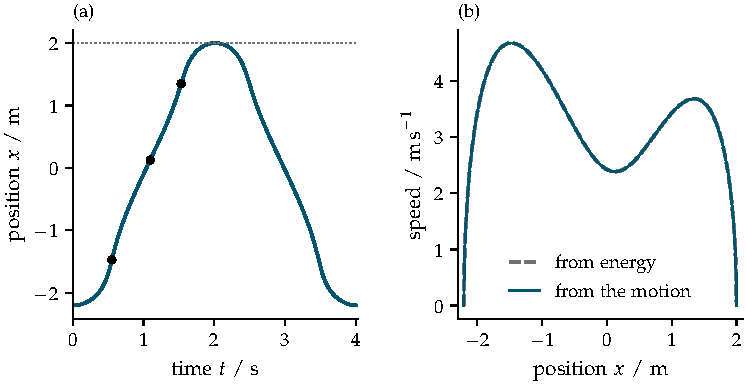
\includegraphics{ch06_lagrange/bead}
\caption{The bead on the wire of \cref{sec:en-track}, released from rest
at $x = \SI{-2.206}{\metre}$, \SI{1.3}{\metre} high, its motion found from
\cref{eq:la-bead}. (a) Its position along $x$ against time, through one
swing to $x = \SI{2}{\metre}$ (dotted) and back; the dots mark the bottom
of the deep valley, the top of the hill and the bottom of the shallow
valley on the way out. (b) Its speed along the wire against $x$ on the way
out, lying on the speed from energy (dashed), which it hides.}
\label{fig:la-bead}
\end{figure}

\subsection*{The pendulum}

With $\Lag = \frac12 mL^2\dot\theta^2 - mgL(1 - \cos\theta)$,
$\partial\Lag/\partial\dot\theta = mL^2\dot\theta$ and $\partial\Lag/
\partial\theta = -mgL\sin\theta$, so \cref{eq:la-euler} gives
$mL^2\ddot\theta = -mgL\sin\theta$, or
\begin{equation}
   \ddot\theta = -\frac{g}{L}\sin\theta ,
   \label{eq:la-pendulum}
\end{equation}
in one line, with the rod's pull nowhere. For small swings $\sin\theta
\approx \theta$ (\cref{sec:mo-taylor}), and $\ddot\theta = -(g/L)\theta$
is the spring of \cref{sec:ne-spring} with $\omega_0 = \sqrt{g/L}$, as
\cref{sec:os-small} found from the energy.

\begin{keyidea}
Constraints that do no work are obeyed by choosing generalised
coordinates, and the Euler--Lagrange equations in those coordinates give
the motion without the constraining forces: for the bead, $\ddot{x} =
-h'(g + h''\dot{x}^2)/(1 + h'^2)$.
\end{keyidea}

\notebook{06}{put the bead on any wire and time its journey}

\begin{selfcheck}
How long does the bead released at \SI{1.3}{\metre} take to go from the
bottom of the deep valley to the bottom of the shallow one?
\end{selfcheck}

%=============================================================================!
% 6.5  POLAR COORDINATES AND CONSERVED MOMENTA                                !
%=============================================================================!
\section{Polar coordinates and conserved momenta}
\label{sec:la-polar}

\Cref{sec:ro-plane} found that a central force conserves angular
momentum, by computing the torque. In polar coordinates the Lagrangian
shows it at a glance, and the same reading gives a general rule: a
coordinate that the Lagrangian does not contain carries a conserved
quantity.

\subsection*{A body pulled towards a centre}

A puck on a smooth table is pulled towards a fixed point, the origin, by a
force that depends only on its distance $r$, with potential energy $U(r)$.
By \cref{eq:ro-polar} its velocity has the parts $\dot{r}$ along the line
to the origin and $r\dot\theta$ across it, at right angles, so its speed
squared is $\dot{r}^2 + r^2\dot\theta^2$ and
\begin{equation*}
   \Lag = \tfrac12 m\,\bigl(\dot{r}^2 + r^2\dot\theta^2\bigr) - U(r) .
\end{equation*}
For the coordinate $\theta$, $\partial\Lag/\partial\dot\theta =
mr^2\dot\theta$, and $\partial\Lag/\partial\theta = 0$, since $\theta$
appears nowhere in $\Lag$. \Cref{eq:la-euler} therefore reads
\begin{equation*}
   \frac{\dd}{\dd t}\bigl(mr^2\dot\theta\bigr) = 0 :
\end{equation*}
the angular momentum $L = mr^2\dot\theta$ of \cref{sec:ro-plane} (not
the rod length $L$ of the pendulum) is conserved.

\subsection*{Conserved momenta}

For any generalised coordinate $q_k$, the quantity
\begin{equation}
   p_k = \frac{\partial\Lag}{\partial\dot{q}_k}
   \label{eq:la-momentum}
\end{equation}
is called the momentum belonging to $q_k$, or its conjugate momentum. For
$x$ in $\Lag = \frac12 m\dot{x}^2 - U$ it is $m\dot{x}$, the momentum of
\cref{sec:ne-bodies}; for $\theta$ above it is the angular momentum. By
\cref{eq:la-euler}, $\dot{p}_k = \partial\Lag/\partial q_k$, so whenever
$\Lag$ does not contain $q_k$ itself, only its rate $\dot{q}_k$, the
momentum $p_k$ is conserved. The Lagrangian of the puck does not contain
$\theta$ because turning the whole picture about the origin changes
nothing; that of a free body does not contain $x$ because moving it
changes nothing. Chapter~7 turns this observation into Noether's theorem,
which ties every such symmetry to a conserved quantity.

\subsection*{The effective potential}

For $r$, $\partial\Lag/\partial\dot{r} = m\dot{r}$ and $\partial\Lag/
\partial r = mr\dot\theta^2 - U'(r)$, so
\begin{align*}
   m\ddot{r} &= mr\dot\theta^2 - U'(r)\\
   &= mr\,\frac{L^2}{m^2r^4} - U'(r)
   && \text{putting in $\dot\theta = L/(mr^2)$, from $L = mr^2\dot\theta$,}\\
   &= \frac{L^2}{mr^3} - U'(r)
   && \text{cancelling $m$ and $r$.}
\end{align*}
Since $L$ is constant, the right side is a function of $r$ alone, and it
is minus the derivative of
\begin{equation}
   U_{\mathrm{eff}}(r) = U(r) + \frac{L^2}{2mr^2} ,
   \label{eq:la-effective}
\end{equation}
because $\dd\bigl(L^2/(2mr^2)\bigr)/\dd r = -L^2/(mr^3)$ by the power rule for
negative powers (\cref{sec:os-anharmonic}). The distance from the origin
therefore moves as a body on a line in the effective potential
$U_{\mathrm{eff}}$, and the energy diagrams of \cref{sec:en-diagrams}
apply to it: $\frac12 m\dot{r}^2 + U_{\mathrm{eff}}(r)$ keeps a fixed
value $E$, and $r$ turns back where $U_{\mathrm{eff}}(r) = E$. This $E$ is
the whole energy $K + U$, since $L^2/(2mr^2) = \frac12 mr^2\dot\theta^2$
is the kinetic energy of the motion across the line. The extra term grows without limit as
$r \to 0$, so for a potential that stays finite at the centre, as the
spring's does, a body that is going round, $L \neq 0$, never reaches the
centre.

Join the puck of \SI{0.2}{\kilogram} to the hole by a spring of
\SI{2}{\newton\per\metre} and natural length zero, so that $U = \frac12
kr^2$, and start it \SI{0.5}{\metre} out, moving across the line to the
hole at \SI{0.5}{\metre\per\second}. Then $L = mrv_\theta = 0.2\times0.5\times0.5 =
\SI{0.05}{\kilogram\metre\squared\per\second}$ and $E = \frac12\times0.2
\times0.5^2 + \frac12\times2\times0.5^2 = \SI{0.275}{\joule}$. The turning
points solve $\frac12 kr^2 + L^2/(2mr^2) = E$. Multiplying by $r^2$ and
moving $Er^2$ across gives $\frac12 kr^4 - Er^2 + L^2/(2m) = 0$, a quadratic
in the unknown $r^2$, with $\frac12 k = 1$ and $L^2/(2m) =
0.05^2/(2\times0.2) = 0.00625$:
\begin{align*}
   r^4 - 0.275\,r^2 + 0.00625 &= 0 ,\\
   r^2 &= \tfrac12\bigl(0.275 \pm\sqrt{0.275^2 - 4\times0.00625}\bigr)\\
   &= \tfrac12\,(0.275 \pm 0.225) = 0.25 \text{ or } 0.025 ,
\end{align*}
by the formula for the roots of a quadratic,
so $r$ swings between $\sqrt{0.025} = \SI{0.1581}{\metre}$ and $\sqrt{0.25}
= \SI{0.5}{\metre}$
(\cref{fig:la-central}). The path, computed with the function
\texttt{solve\_newton}, is an ellipse centred on the hole between these
two distances.

\begin{figure}[htb]
\centering
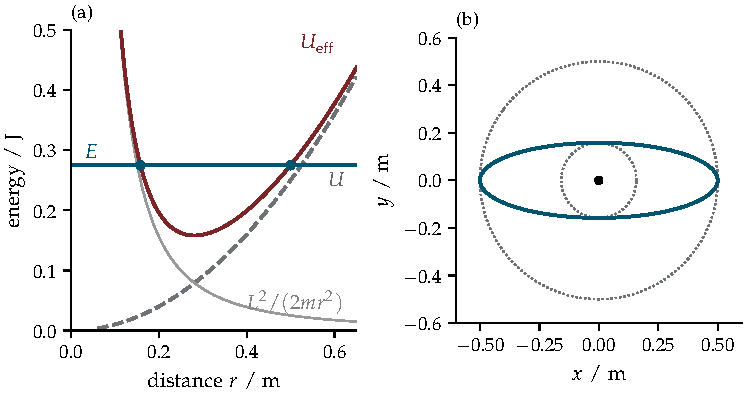
\includegraphics{ch06_lagrange/central}
\caption{A puck of \SI{0.2}{\kilogram} joined to a hole by a spring of
\SI{2}{\newton\per\metre}, started \SI{0.5}{\metre} out at
\SI{0.5}{\metre\per\second} across the line to the hole. (a) The
potential energy $U$, the term $L^2/(2mr^2)$ and their sum, the effective
potential, with the energy $E$; the dots are the turning points. (b) The
path seen from above, between circles at the two turning distances.}
\label{fig:la-central}
\end{figure}

The $r$ equation also gives the pull of the string in \cref{fig:ro-puck}.
A pull of size $F$ towards the hole is the force $-F$ along $\vb{e}_r$ and
takes the place of $-U'(r)$: a pull $F(t)$ acts as the potential $F(t)\,r$
at each instant, and the derivation of \cref{sec:la-euler} compares paths
instant by instant, so it still applies, so $m\ddot{r} = mr\dot\theta^2 - F$. There the
puck was drawn in at a steady speed, $\ddot{r} = 0$, so $F = mr\dot
\theta^2 = L^2/(mr^3)$, the pull with which \cref{fig:ro-puck} was
computed.

\begin{keyidea}
The momentum belonging to a coordinate is $p_k = \partial\Lag/\partial
\dot{q}_k$, and it is conserved when $\Lag$ does not contain $q_k$. For a
central force, $\theta$ is such a coordinate and its momentum is the
angular momentum; the distance $r$ then moves in the effective potential
$U + L^2/(2mr^2)$.
\end{keyidea}

\notebook{06}{explore the effective potential and the paths it gives}

\begin{selfcheck}
For $\Lag = \frac12 m(\dot{x}^2 + \dot{y}^2) - mgy$, a ball thrown in a
vertical plane, which momentum is conserved, and why?
\end{selfcheck}

%=============================================================================!
% 6.6  CONSTRAINTS AND LAGRANGE MULTIPLIERS                                   !
%=============================================================================!
\section{Constraints and Lagrange multipliers}
\label{sec:la-multipliers}

Choosing coordinates that obey a constraint makes its force disappear,
which is what we want when only the motion matters. Sometimes the force
itself is wanted, such as the tension of a pendulum's rod, and sometimes no
convenient coordinates exist, as for the bonds of a large molecule held at
fixed lengths. Then we keep the Cartesian coordinates and let the
constraint enter through a new unknown, a Lagrange multiplier. This
section introduces the tool, uses it on the pendulum, and compares the
result with Newton's laws.

\begin{toolbox}[Lagrange multipliers]
Suppose we want the largest or smallest value of $f(x, y)$ among the
points on the curve $\chi(x, y) = 0$, written with the Greek chi since $g$
is the acceleration of free fall. Move along the curve, in the direction
of a short arrow $\vb{u}$ along it. By the chain rule along a path
(\cref{sec:en-gradient}), $f$ changes at the rate $\grad f\cdot\vb{u}$,
and $\chi$ at the rate $\grad\chi\cdot\vb{u} = 0$, since $\chi$ stays zero
on the curve. At a largest or smallest value of $f$ on the curve its rate
of change along the curve is zero too, $\grad f\cdot\vb{u} = 0$. In the
plane there is only one direction at right angles to $\vb{u}$, so $\grad
f$ and $\grad\chi$, the latter not zero, point along the same line there:
\begin{equation*}
   \grad f = \lambda\,\grad\chi , \qquad \chi = 0 ,
\end{equation*}
for some number $\lambda$, called the Lagrange multiplier: three equations
for the three unknowns $x$, $y$ and $\lambda$. For example, the rectangle
of largest area $f = xy$ with a perimeter of \SI{4}{\metre}, $\chi = 2x +
2y - 4 = 0$, has $(y, x) = \lambda\,(2, 2)$, so $x = y$, and the perimeter
gives $x = y = \SI{1}{\metre}$: a square. With more variables the same
argument, applied to every arrow $\vb{u}$ along the surface $\chi = 0$,
again puts $\grad f$ along $\grad\chi$; with several constraints $\chi_c =
0$, one multiplier $\lambda_c$ each, it becomes $\grad f =
\sum_c\lambda_c\grad\chi_c$, which we take on trust.
\end{toolbox}

Here $\lambda$ is a multiplier, not the eigenvalue of \cref{sec:os-modes}.

\subsection*{The pendulum in $x$ and $y$}

Describe the bob by its Cartesian position $\vb{r} = (x, y)$, with the
pivot at the origin and $y$ up, and impose the rod as the constraint $\chi
= \frac12(x^2 + y^2 - L^2) = 0$. Its gradient is $\grad\chi = (x, y) =
\vb{r}$, along the rod and at right angles to the circle $\chi = 0$, as a
gradient is to its contour (\cref{sec:en-gradient}). The rod does no work
(\cref{sec:la-coordinates}), so its force too is at right angles to the
circle, along $\grad\chi$: it is $\lambda\,\grad\chi = \lambda\vb{r}$ for
some multiplier $\lambda$ that may change with time, and Newton's second
law reads
\begin{equation*}
   m\ddot{\vb{r}} = m\vb{g} + \lambda\vb{r} ,
\end{equation*}
with $\vb{g} = (0, -g)$ the acceleration of free fall.

Hamilton's principle gives the same equation, and shows where the
multiplier comes from. Here $\Lag = \frac12 m(\dot{x}^2 + \dot{y}^2) -
mgy$. Changing the path by $\zeta\boldsymbol{\eta}(t)$, with
$\boldsymbol{\eta} = (\eta_x, \eta_y)$ zero at both ends, the steps of
\cref{sec:la-euler}, once for $x$ and once for $y$, change the action by
$\zeta\int\vb{B}\cdot\boldsymbol{\eta}\,\dd t$ plus terms of order
$\zeta^2$, where
\begin{equation*}
   \vb{B} = \Bigl(\frac{\partial\Lag}{\partial x}
   - \frac{\dd}{\dd t}\frac{\partial\Lag}{\partial\dot{x}},\
   \frac{\partial\Lag}{\partial y}
   - \frac{\dd}{\dd t}\frac{\partial\Lag}{\partial\dot{y}}\Bigr)
   = \bigl(-m\ddot{x},\ -mg - m\ddot{y}\bigr)
   = m\vb{g} - m\ddot{\vb{r}} .
\end{equation*}
Among all paths this would give $\vb{B} = \vb{0}$, the bob falling freely.
Only paths that keep the bob on its circle are allowed, so at each instant
$\boldsymbol{\eta}$ must point along the circle, $\boldsymbol{\eta} =
\eta(t)\,\vb{e}_\theta$ with $\vb{e}_\theta$ the arrow of length one along
the circle at the bob (\cref{eq:ro-polar}); such a change alters the length only by terms in $\zeta^2$, which
do not touch the term in $\zeta$. The change of action is then
$\zeta\int(\vb{B}\cdot\vb{e}_\theta)\,\eta\,\dd t$, and the bump argument
of \cref{sec:la-euler} gives $\vb{B}\cdot\vb{e}_\theta = 0$ at every
instant:
$\vb{B}$ has no part along the circle. In the plane only the direction of
$\vb{r}$ is left, as in the toolbox, so $\vb{B} = -\lambda\vb{r}$ for some
number $\lambda$ at each instant, the minus sign only a choice of name,
and $m\vb{g} - m\ddot{\vb{r}} = -\lambda\vb{r}$ is the second law above.
The constraint leaves the principle silent about one force, along
$\grad\chi$, and that force is the rod's. Equivalently, these are the
Euler--Lagrange equations of $\Lag + \lambda\chi$ in $x$ and $y$ treated
as free, the usual way of writing a multiplier, with one $\lambda$ for
each instant.

The multiplier is fixed by the constraint itself. Differentiating
$\vb{r}\cdot\vb{r} = x^2 + y^2 = L^2$ twice with respect to time, by the
product rule on each component as in \cref{sec:mo-circle},
\begin{align*}
   2\,\vb{r}\cdot\dot{\vb{r}} &= 0 ,\\
   \dot{\vb{r}}\cdot\dot{\vb{r}} + \vb{r}\cdot\ddot{\vb{r}} &= 0
   && \text{differentiating again and halving,}\\
   \lvert\vb{v}\rvert^2 + \vb{r}\cdot\vb{g} + \frac{\lambda}{m}\,L^2 &= 0
   && \text{putting in $\ddot{\vb{r}} = \vb{g} + (\lambda/m)\vb{r}$ and
      $\vb{r}\cdot\vb{r} = L^2$,}
\end{align*}
so
\begin{equation}
   \lambda = -\frac{m\,\bigl(\lvert\vb{v}\rvert^2 + \vb{r}\cdot\vb{g}
   \bigr)}{L^2} .
   \label{eq:la-multiplier}
\end{equation}
The function \texttt{rod\_multiplier} of \texttt{mdlab} evaluates it. The
rod's force $\lambda\vb{r}$ is $-\lambda L$ times $-\vb{r}/L$, the arrow of
length one from the bob to the pivot, so the rod pulls the bob towards the
pivot with the force $F_{\mathrm{rod}} = -\lambda L$, which is negative
when the rod pushes. With the bob at the angle $\theta$ from the vertical,
$\vb{r} = L(\sin\theta, -\cos\theta)$, so $\vb{r}\cdot\vb{g} =
gL\cos\theta$, and $\lvert\vb{v}\rvert = L\lvert\dot\theta\rvert$
(\cref{sec:la-coordinates}). Then
\begin{equation*}
   F_{\mathrm{rod}} = -\lambda L
   = \frac{m\,\bigl(L^2\dot\theta^2 + gL\cos\theta\bigr)}{L}
   = m\,\bigl(g\cos\theta + L\dot\theta^2\bigr) :
\end{equation*}
the part of the weight along the rod plus the inward pull $mL\dot\theta^2$
that going round a circle needs (\cref{sec:mo-circle}).

Released from rest at the angle $\theta_0$, the bob keeps its energy $K +
U$ of \cref{sec:la-coordinates} at its starting value $mgL(1 -
\cos\theta_0)$, so $\frac12 mL^2\dot\theta^2 = mgL(1 - \cos\theta_0) -
mgL(1 - \cos\theta) = mgL(\cos\theta - \cos\theta_0)$; multiplying by
$2/(mL)$, $L\dot\theta^2 = 2g(\cos\theta - \cos\theta_0)$ and
\begin{equation*}
   F_{\mathrm{rod}} = mg\,(3\cos\theta - 2\cos\theta_0) .
\end{equation*}
\Cref{fig:la-tension} follows a bob of \SI{0.5}{\kilogram} on a rod of
\SI{1.2}{\metre} released from \ang{120}, computed in $x$ and $y$ with the
multiplier: the length stays \SI{1.2}{\metre} to within \SI{1e-11}{\metre},
and the force agrees with the formula at every angle: at the bottom it is
$mg\,(3 - 2\cos\ang{120}) = mg\,(3 + 1) = 4mg = 4\times0.5\times9.80665 =
\SI{19.613}{\newton}$. It is negative where $3\cos\theta < 2\cos\theta_0$,
beyond $\cos\theta = \frac23\cos\theta_0 = -\frac13$, here beyond
\ang{109.47}: the rod pushes the bob outwards. A string, which can only
pull, could not follow this swing at all: at the release point the force
needed is $mg\cos\ang{120} = -\frac12 mg$, a push, so a string is slack
from the start. \Cref{ex:la-slack} shows that a string stays taut only for
swings of at most \ang{90}, the limit of \cref{sec:os-anharmonic}. The
angle \ang{109.47} belongs to this swing of \ang{120}: between \ang{90} and
\ang{109.47} the bob, though above the pivot, moves fast enough that the
rod still pulls.

\begin{figure}[htb]
\centering
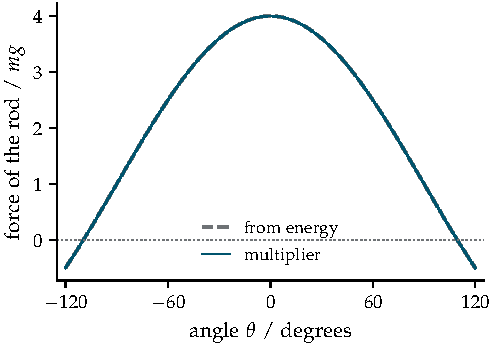
\includegraphics{ch06_lagrange/tension}
\caption{The force of the rod on a pendulum's bob of \SI{0.5}{\kilogram}
on a rod of \SI{1.2}{\metre}, released from rest at \ang{120}, divided by
the bob's weight, against the angle over one swing: from the Lagrange
multiplier of the constraint (solid) and from energy, $3\cos\theta - 2\cos
\theta_0$ (dashed), which the solid line hides. Below the dotted line the
rod pushes.}
\label{fig:la-tension}
\end{figure}

\subsection*{Bonds of fixed length}

A bond held at the length $d$ between atoms $i$ and $j$ is the constraint
$\chi = \frac12(\lvert\vb{r}_j - \vb{r}_i\rvert^2 - d^2) = 0$. Its gradient
with respect to $\vb{r}_j$ is $\vb{r}_j - \vb{r}_i$, and with respect to
$\vb{r}_i$ it is $-(\vb{r}_j - \vb{r}_i)$ (\cref{ex:la-bond}), so the
multiplier gives the two atoms equal and opposite forces along the bond, as
the third law requires. Freezing the fastest bonds of a molecule this
way, those to hydrogen, whose periods of \SI{9}{\femto\second} for O--H and
\SI{11}{\femto\second} for C--H limit the step of a simulation (\cref{sec:os-molecules}), lets the steps grow;
Chapter~11 finds the multipliers at every step with the method called
SHAKE.

\begin{keyidea}
To find the largest or smallest value of $f$ subject to $\chi = 0$, solve
$\grad f = \lambda\grad\chi$ with $\chi = 0$. In mechanics a constraint $\chi = 0$
that does no work enters as the force $\lambda\grad\chi$, and $\lambda$,
fixed by differentiating the constraint twice, measures the force needed
to keep it: for a pendulum it gives the force of the rod, $-\lambda L$.
\end{keyidea}

\notebook{06}{the pendulum in $x$ and $y$ with its multiplier}

\begin{selfcheck}
A pendulum is released from rest at \ang{90}. What force does the rod
exert at the bottom of the swing, in units of the bob's weight?
\end{selfcheck}

%=============================================================================!
% 6.S  WHAT WE NOW HAVE                                                       !
%=============================================================================!
\unnumbered{What we now have}

Mechanics can be written in any coordinates that fix the positions of a
system once its constraints are obeyed, its generalised coordinates, with
the Lagrangian $\Lag = K - U$ expressed in them. Among all paths with the
same ends in space and time, the true one makes the action $\Act = \int
\Lag\,\dd t$ stationary, which is not always least. Changing a path by a
small bump and integrating by parts turns this into the Euler--Lagrange
equations, $\dd(\partial\Lag/\partial\dot{q}_k)/\dd t = \partial\Lag/
\partial q_k$, one for each coordinate, which for forces from a potential
are Newton's second law.

Constraints that do no work drop out of $\Lag$:
solving the bead's equation along its wire gives the times of the journey
that Chapter~3 described by its speeds, and the pendulum's equation takes
one line.

The momentum $p_k = \partial\Lag/\partial\dot{q}_k$ of a
coordinate that $\Lag$ does not contain is conserved, which is why a
central force conserves angular momentum; the distance from the centre
then moves in the effective potential $U + L^2/(2mr^2)$.

When a
constraining force is wanted, or no convenient coordinates exist, a Lagrange multiplier keeps the constraint: for a pendulum it gives the
force of the rod, $-\lambda L$, and for bonds held at fixed length the
multipliers are what Chapter~11 computes at every step.

Chapter~7 trades the generalised velocities for the momenta and arrives at
Hamilton's equations, the form of mechanics on which the methods of
simulation are built.

%=============================================================================!
% 6.A  ANSWERS TO THE CHECKS                                                  !
%=============================================================================!
\unnumbered{Answers to the checks}
\label{sec:la-answers}

\answerto{sec:la-coordinates}The double pendulum in a plane needs the two
angles of its rods, 2 coordinates. The rigid diatomic molecule needs the
three coordinates of its centre of mass and two angles for the direction
of its bond, 5, the $3N - 1$ left when one distance of $N = 2$ atoms is
fixed.

\answerto{sec:la-action}With $U = 0$ the expansion of the action has only
the kinetic terms: $\Act(\zeta) = \Act(0) + \zeta\int m\dot{x}\dot\eta\,
\dd t + \zeta^2\,\frac12 m\int\dot\eta^2\,\dd t$. On the straight path
$\dot{x}$ is constant, so the middle term is $m\dot{x}\,[\eta]_{t_1}^{t_2}
= 0$, the bump being zero at both ends. The last term is positive unless
$\dot\eta = 0$ throughout, which with $\eta$ zero at the ends means no
change at all. Any other path with the same ends is the straight one plus such a change,
with $\zeta = 1$ and $\eta$ the difference, and with $U = 0$ the expansion
is exact, so every other path has more action.

\answerto{sec:la-euler}$\partial\Lag/\partial\dot{x} = m\dot{x}$ and
$\partial\Lag/\partial x = -kx$, so $m\ddot{x} = -kx$, the equation of
\cref{sec:ne-spring}.

\answerto{sec:la-constrained}From \SI{0.554}{\second} to
\SI{1.533}{\second}, that is $1.533 - 0.554 = \SI{0.979}{\second}$.

\answerto{sec:la-polar}$\Lag$ does not contain $x$, only $\dot{x}$, so
$p_x = \partial\Lag/\partial\dot{x} = m\dot{x}$ is conserved: nothing
pushes the ball sideways. It does contain $y$, through $mgy$, so $p_y =
m\dot{y}$ changes, at the rate $\partial\Lag/\partial y = -mg$, the weight.

\answerto{sec:la-multipliers}With $\theta_0 = \ang{90}$, $\cos\theta_0 =
0$, and at the bottom $\cos\theta = 1$, so $F_{\mathrm{rod}} = mg(3 - 0) =
3mg$, three times the weight.

%=============================================================================!
% 6.E  EXERCISES                                                              !
%=============================================================================!
\unnumbered{Exercises}
\label{sec:la-exercises}

The exercises run from questions of understanding, through calculations,
to short derivations marked `show that'. Full solutions are in
\hyperref[sec:la-solutions]{`Solutions to the exercises'} at the end of
the book, and Notebook~06 checks every numerical answer.

\begin{exercise}[counting coordinates]
\label{ex:la-count}
How many generalised coordinates do (a) a bead threaded on a fixed
circular hoop, (b) two atoms joined by a rigid bond and moving in a plane,
and (c) a rigid water molecule free in space have?
\end{exercise}

\begin{exercise}[by parts]
\label{ex:la-parts}
Find $\int_0^1 x\,\mathrm{e}^x\,\dd x$ by integration by parts.
\end{exercise}

\begin{exercise}[a saddle of the action]
\label{ex:la-saddle}
For the block of \cref{sec:la-action} ($m = \SI{0.5}{\kilogram}$, $k =
\SI{50}{\newton\per\metre}$) over $\tau = \SI{0.5}{\second}$, show that
adding the bump $\zeta\sin(n\pi t/\tau)$ to the true path changes the
action by $\zeta^2(\tau/4)\bigl(m(n\pi/\tau)^2 - k\bigr)$, and evaluate the
coefficient of $\zeta^2$ for $n = 1$ and 2.
\end{exercise}

\begin{exercise}[free fall]
\label{ex:la-fall}
Write the Euler--Lagrange equation for $\Lag = \frac12 m\dot{x}^2 - mgx$.
\end{exercise}

\begin{exercise}[two coordinates]
\label{ex:la-plane}
Show that for $\Lag = \frac12 m(\dot{x}^2 + \dot{y}^2) - U(x, y)$ the two
Euler--Lagrange equations are Newton's second law for the two components
of the force $-\grad U$.
\end{exercise}

\begin{exercise}[the bottom of a valley]
\label{ex:la-valley}
Show that near the bottom $x_0$ of a valley of the wire, where $h'(x_0) =
0$, \cref{eq:la-bead} becomes $\ddot{x} \approx -g\,h''(x_0)\,(x - x_0)$,
and hence that small swings have $\omega_0 = \sqrt{g\,h''(x_0)}$, as
\cref{sec:os-small} found.
\end{exercise}

\begin{exercise}[a bead in a bowl]
\label{ex:la-bowl}
A bead slides in a circular bowl, $h(x) = R - \sqrt{R^2 - x^2}$. Show
that with $x = R\sin\theta$ its Lagrangian becomes that of a pendulum of
length $R$.
\end{exercise}

\begin{exercise}[energy from the equation]
\label{ex:la-energy}
Multiplying \cref{eq:la-pendulum} by $\dot\theta$, show that $\frac12
mL^2\dot\theta^2 + mgL(1 - \cos\theta)$ does not change.
\end{exercise}

\begin{exercise}[the energy of a Lagrangian]
\label{ex:la-hamilton}
For a Lagrangian $\Lag(q, \dot{q})$ of one coordinate that does not
contain the time, show from \cref{eq:la-euler} that $\dot{q}\,\partial
\Lag/\partial\dot{q} - \Lag$ does not change along the motion, and that
for the bead it equals $K + U$.
\end{exercise}

\begin{exercise}[two carts]
\label{ex:la-carts}
Two carts of masses $m_1$ and $m_2$ on a smooth track are joined by a
spring, $\Lag = \frac12 m_1\dot{x}_1^2 + \frac12 m_2\dot{x}_2^2 - \frac12
k(x_2 - x_1 - \ell)^2$. Rewrite it with the centre of mass $X = (m_1x_1 +
m_2x_2)/(m_1 + m_2)$ and the separation $r = x_2 - x_1$, and show that
the momentum belonging to $X$ is conserved and that $r$ moves with the
reduced mass of \cref{sec:os-bodies}.
\end{exercise}

\begin{exercise}[turning points]
\label{ex:la-turning}
The puck of \cref{fig:la-central} is started \SI{0.4}{\metre} out at
\SI{0.3}{\metre\per\second} across the line to the hole. Find $L$, $E$
and the two distances between which it swings.
\end{exercise}

\begin{exercise}[going round in a circle]
\label{ex:la-circle}
For $U = \frac12 kr^2$, show that the puck goes round in a circle when
$r^4 = L^2/(mk)$, and that it then turns at the angular speed
$\sqrt{k/m}$, whatever $L$. Evaluate the radius for the puck of
\cref{fig:la-central}, of \SI{0.2}{\kilogram} on a spring of
\SI{2}{\newton\per\metre}, with $L = \SI{0.05}{\kilogram\metre\squared\per
\second}$.
\end{exercise}

\begin{exercise}[on the unit circle]
\label{ex:la-unit}
Find the largest value of $xy$ on the circle $x^2 + y^2 = 1$, and where
it is reached.
\end{exercise}

\begin{exercise}[a deep swing]
\label{ex:la-swing}
A bob of \SI{0.5}{\kilogram} on a rod is released from rest at \ang{60}.
What is the force of the rod when the bob passes the bottom, and when it
is released?
\end{exercise}

\begin{exercise}[when a string goes slack]
\label{ex:la-slack}
Show that a pendulum on a string released from rest at $\theta_0$ keeps
its string taut throughout only if $\theta_0 \le \ang{90}$.
\end{exercise}

\begin{exercise}[the forces of a bond]
\label{ex:la-bond}
For $\chi = \frac12(\lvert\vb{r}_j - \vb{r}_i\rvert^2 - d^2)$, show that
$\grad_j\chi = \vb{r}_j - \vb{r}_i$ and $\grad_i\chi = -(\vb{r}_j -
\vb{r}_i)$, so that the forces $\lambda\grad_i\chi$ and $\lambda\grad_j
\chi$ on the two atoms are equal, opposite and along the bond.
\end{exercise}

\begin{exercise}[a smaller swing]
\label{ex:la-small-swing}
The bead of \cref{sec:la-constrained} is released from rest on the left
slope at a height of \SI{0.8}{\metre}. Using \texttt{solve\_wire} in
Notebook~06, find where it turns and how long it takes to come back.
\end{exercise}


%=============================================================================!
% CHAPTER 7  HAMILTONIAN MECHANICS AND PHASE SPACE                            !
%=============================================================================!
\chapter{Hamiltonian mechanics and phase space}
\label{ch:hamilton}

%=============================================================================!
% 7.0  CHAPTER OPENING                                                        !
%=============================================================================!
Chapter~6 described motion through generalised coordinates and their
velocities, and introduced the conjugate momentum belonging to each
coordinate. We now use those momenta in place of the velocities. This
change leads to Hamilton's equations and makes the state of a system a
point in phase space, the space of all allowed coordinates and momenta.
Following many starting states at once reveals properties of the motion
that are difficult to see from a single trajectory.

For the time-independent systems considered here, the flow preserves
energy as well as the area, or in more dimensions the volume, of a region
of states. We derive this volume conservation as Liouville's theorem,
which Chapter~12 needs for statistical mechanics. We then connect spatial
symmetries to conserved momenta and establish the conditions under which
reversing momenta retraces a trajectory. These results give us concrete
tests for a numerical method: the final section compares two simple step
maps, preparing the integration methods of Chapter~9.

%=============================================================================!
% 7.1  FROM VELOCITIES TO MOMENTA                                             !
%=============================================================================!
\section{From velocities to momenta}
\label{sec:ha-legendre}

The state of the bead on its wire (\cref{sec:la-coordinates}) is its
position $x$ and its rate $\dot{x}$, but it can equally be given by $x$
and the momentum $p = \partial\Lag/\partial\dot{x}$ of
\cref{eq:la-momentum}, which for the bead is $m(1 + h'^2)\dot{x}$
(\cref{sec:la-constrained}): since $1 + h'^2$ is positive, each $\dot{x}$ gives
one $p$, and $\dot{x} = p/\bigl(m(1 + h'^2)\bigr)$ gives the rate back.
Hamilton's form of mechanics describes the state by the coordinates and
their momenta. \Cref{sec:ha-liouville} shows that
the motion keeps areas in the plane of $q$ and $p$, which it does not in
general do in the plane of $q$ and $\dot{q}$. The new description needs a
function of $q$ and $p$ that does the work that $\Lag$ does for $q$ and
$\dot{q}$. The tool that exchanges a variable for the slope of a function
of it is the Legendre transform.

\begin{toolbox}[The Legendre transform]
Let $f(v)$ be a function whose slope $f'(v)$ grows steadily with $v$,
that is $f''(v) > 0$ (its graph curves upwards). Then each slope $p$ is
reached at no more than one value of $v$, and we take $p$ among the slopes
that $f$ has. The straight line $pv$ through the origin has that slope
(\cref{fig:ha-legendre}a). The gap between line and
curve, $pv - f(v)$, changes at the rate $p - f'(v)$ as $v$ grows: the
rate is positive while $f'(v) < p$ and negative once $f'(v) > p$, so the
gap rises to its largest value at the $v$ where $f'(v) = p$ and falls
after it. That largest gap is the Legendre transform of $f$,
\begin{equation*}
   f^*(p) = pv - f(v) , \qquad\text{with $v$ such that } f'(v) = p .
\end{equation*}
The tangent to $f$ at that $v$ has slope $p$ and passes through $(v,
f(v))$, so at the vertical axis, a distance $v$ to the left, it is at
$f(v) - pv = -f^*(p)$: the transform is where the tangent of slope $p$
meets the axis, with its sign reversed.

As $p$ changes, $v$ changes with it. By the product rule and the chain
rule,
\begin{align*}
   \frac{\dd f^*}{\dd p}
   &= v + p\,\frac{\dd v}{\dd p} - f'(v)\,\frac{\dd v}{\dd p}
   && \text{differentiating $pv$ and $f(v(p))$}\\
   &= v
   && \text{since $f'(v) = p$ cancels the last two terms.}
\end{align*}
The slope of $f^*$ is $v$, as the slope of $f$ is $p$
(\cref{fig:ha-legendre}b). This slope grows with $p$: differentiating $f'\bigl(v(p)\bigr) = p$ with
respect to $p$ by the chain rule gives $f''(v)\,\dd v/\dd p = 1$, so $\dd
v/\dd p = 1/f''(v) > 0$, as for the inverse functions of
\cref{sec:os-anharmonic}. So $f^*$ can be transformed in its turn. Its
transform at the slope $v$ is $vp - f^*(p)$, with $p$ the slope of $f$ at
which the slope of $f^*$ equals $v$, which is the $p = f'(v)$ we started
from, and
\begin{equation*}
   vp - f^*(p) = vp - \bigl(pv - f(v)\bigr) = f(v) :
\end{equation*}
the transform of the transform is the function we started from, so
$f^*$ carries the same information as $f$, written in terms of the slope.
For example, $f(v) = \frac12 mv^2$ has $f'(v) = mv$, so $p = mv$ and $v =
p/m$, and
\begin{align*}
   f^*(p) &= p\,\frac{p}{m} - \frac12 m\Bigl(\frac{p}{m}\Bigr)^2
   && \text{putting $v = p/m$ into $pv - f(v)$}\\
   &= \frac{p^2}{m} - \frac{p^2}{2m} = \frac{p^2}{2m} ,
\end{align*}
whose slope $p/m$ is indeed $v$.
\end{toolbox}

\begin{figure}[htb]
\centering
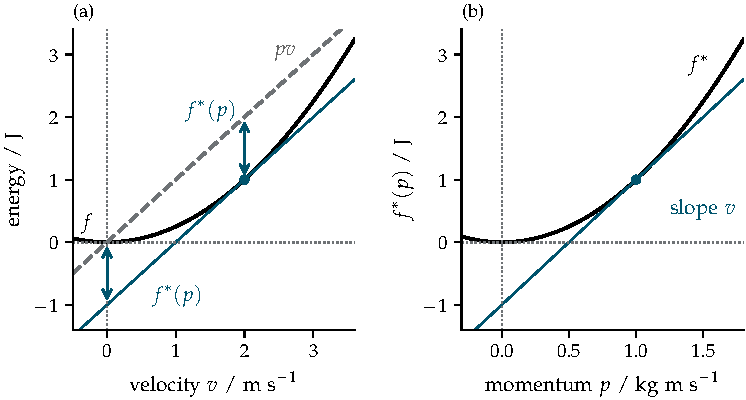
\includegraphics{ch07_hamilton/legendre}
\caption{The Legendre transform of $f(v) = \frac12 mv^2$ for a body of
\SI{0.5}{\kilogram}. (a) The line $pv$ with $p =
\SI{1}{\kilogram\metre\per\second}$ (dashed) differs from $f$ by $pv -
f(v)$, which is largest, $f^*(p) = \SI{1}{\joule}$, at $v = p/m =
\SI{2}{\metre\per\second}$, where the slope of $f$ is $p$; the tangent
there (teal) meets the vertical axis at $-f^*(p)$. (b) The transform
$f^*(p) = p^2/(2m)$, whose slope at $p$ is $v$.}
\label{fig:ha-legendre}
\end{figure}

\subsection*{The Hamiltonian}

For one coordinate, the Lagrangian $\Lag(q, \dot{q})$ is a function of
$\dot{q}$ at each fixed $q$, and its slope in $\dot{q}$ is the momentum.
Its Legendre transform in $\dot{q}$, with $q$ held fixed throughout, is
the Hamiltonian,
\begin{equation}
   H(q, p) = p\,\dot{q} - \Lag(q, \dot{q}) ,
   \qquad\text{with $\dot{q}$ such that }
   \frac{\partial\Lag}{\partial\dot{q}} = p ,
   \label{eq:ha-hamiltonian}
\end{equation}
written in terms of $q$ and $p$ alone by putting in $\dot{q}$ found from
$p$; for several coordinates it is $H = \sum_k p_k\dot{q}_k - \Lag$. The
transform needs $\partial\Lag/\partial\dot{q}$ to grow steadily with
$\dot{q}$, which holds for every system met so far, because the kinetic
energy is $K = \frac12 a(q)\,\dot{q}^2$ with a positive $a$: $m$ for a
body on a line, $m(1 + h'^2)$ for the bead, $mL^2$ for the pendulum.

For such a system $p = \partial\Lag/\partial\dot{q} = a\dot{q}$, since $U$
does not contain $\dot{q}$, so $p\dot{q} = a\dot{q}^2 = 2K$, and
\begin{equation*}
   H = 2K - (K - U) = K + U :
\end{equation*}
the Hamiltonian is the energy, now written in terms of the momentum. It
is the quantity $\dot{q}\,\partial\Lag/\partial\dot{q} - \Lag$ that
\cref{ex:la-hamilton} found to be conserved. With several coordinates,
when $K$ is a sum of terms $K_k = \frac12 a_k\dot{q}_k^2$, one for each,
every term gives $p_k\dot{q}_k = a_k\dot{q}_k^2 = 2K_k$, and adding them
again $H = K + U$; \cref{ex:ha-cross}
shows that a kinetic energy with a product of two rates gives the same
result. The examples of Chapter~6 become
\begin{align*}
   &\text{a block on a spring:}
   && p = m\dot{x} ,
   && H = \frac{p^2}{2m} + \frac12 kx^2 ,\\
   &\text{the pendulum:}
   && p = mL^2\dot\theta ,
   && H = \frac{p^2}{2mL^2} + mgL(1 - \cos\theta) ,\\
   &\text{the bead:}
   && p = m(1 + h'^2)\dot{x} ,
   && H = \frac{p^2}{2m\bigl(1 + h'(x)^2\bigr)} + mg\,h(x) ,
\end{align*}
each kinetic energy following from $K = \frac12 a\dot{q}^2$ with $\dot{q}
= p/a$, which gives $K = \frac12 a(p/a)^2 = p^2/(2a)$. The pendulum's
momentum is its angular momentum about the pivot (\cref{sec:ro-plane}).
The bead's kinetic energy now depends on $x$ as well as on $p$, because
the same momentum means a faster bead where the wire is flat than where
it is steep.

For $N$ atoms, with $\vb{p}_i = m_i\dot{\vb{r}}_i$,
\begin{equation*}
   H(\vb{r}^N, \vb{p}^N) = \sum_{i=1}^{N}\frac{\lvert\vb{p}_i\rvert^2}
   {2m_i} + U(\vb{r}^N) ,
\end{equation*}
and the state is the point $\Gamma = (\vb{r}^N, \vb{p}^N)$ of $6N$
numbers. For the puck of \cref{sec:la-polar}, \cref{ex:ha-puck} finds
$H = p_r^2/(2m) + p_\theta^2/(2mr^2) + U(r)$, in which the effective
potential of Chapter~6 appears with $p_\theta$ as the angular momentum $L$
of \cref{sec:la-polar}, not the rod length.

\begin{bridge}
The same transform links the thermodynamic potentials. The free energy of
the electrons at a fixed number $N_{\mathrm{e}}$ has the slope $\mu$, the
chemical potential, with respect to $N_{\mathrm{e}}$; its Legendre
transform in $N_{\mathrm{e}}$, with the sign reversed, is the grand
potential, the free energy minus $\mu N_{\mathrm{e}}$, which is a function
of $\mu$. Grand-canonical DFT holds the electrode's chemical potential
fixed and lets $N_{\mathrm{e}}$ follow, so it minimises the grand
potential, the transform, at fixed $\mu$, as Hamilton's form of mechanics
holds $p$ as the variable in place of $\dot{q}$.
\end{bridge}

\begin{keyidea}
The Hamiltonian $H(q, p) = \sum_k p_k\dot{q}_k - \Lag$ is the Legendre
transform of the Lagrangian in the velocities, written in terms of the
coordinates and the momenta. When the kinetic energy is quadratic in the
velocities it is the energy, $H = K + U$.
\end{keyidea}

\begin{selfcheck}
Write the Hamiltonian of a block of \SI{2}{\kilogram} on a spring of
\SI{8}{\newton\per\metre}. If its energy is \SI{1}{\joule}, what is its
momentum as it passes $x = 0$?
\end{selfcheck}

%=============================================================================!
% 7.2  HAMILTON'S EQUATIONS                                                   !
%=============================================================================!
\section{Hamilton's equations}
\label{sec:ha-equations}

The Hamiltonian is built from the Lagrangian, so the Euler--Lagrange
equation must be expressible through it. Finding how needs the partial
derivatives of $H$, and these differ from those of $\Lag$ in what is held
fixed: $\partial\Lag/\partial q$ is taken at fixed $\dot{q}$, while
$\partial H/\partial q$ is taken at fixed $p$, and at fixed $p$ the rate
$\dot{q}$ changes with $q$. The chain rule of \cref{sec:en-gradient}
keeps track of this once it is stated for functions of several
variables that themselves depend on several others.

\begin{toolbox}[The chain rule in general]
Let $f(x, y)$ depend on two variables, and let these depend in turn on
two others, $x(s, t)$ and $y(s, t)$. Holding $s$ fixed and letting $t$
change moves the point $(x, y)$ along a path, so the chain rule along a
path (\cref{sec:en-gradient}) gives
\begin{equation*}
   \frac{\partial f}{\partial t} = \frac{\partial f}{\partial x}\,
   \frac{\partial x}{\partial t} + \frac{\partial f}{\partial y}\,
   \frac{\partial y}{\partial t} ,
\end{equation*}
where every derivative with respect to $t$ is taken at fixed $s$, and
$\partial f/\partial x$ and $\partial f/\partial y$ are evaluated at the
point $\bigl(x(s, t), y(s, t)\bigr)$. Holding $t$ fixed instead gives
the same with $s$ in place of $t$, and with more variables there is one
term for each variable of $f$. For example, $f = x^2y$ with $x = s + t$
and $y = s - t$ has
\begin{equation*}
   \frac{\partial f}{\partial t} = 2xy\times1 + x^2\times(-1)
   = 2(s + t)(s - t) - (s + t)^2 ,
\end{equation*}
which is what differentiating $f = (s + t)^2(s - t)$ directly with respect
to $t$ gives, by the product rule. A partial derivative is only defined
once we say which variables are held fixed: $\partial f/\partial x$ at
fixed $y$ is $2xy$, but if $y$ were written as $s - t$ and $x$ as $s + t$
and we asked how $f$ changes with $x$ at fixed $s$, so that $y = 2s - x$
changes too, then $f = x^2(2s - x)$ and the answer would be $2x(2s - x) -
x^2 = 2xy - x^2$, which differs from $2xy$.
\end{toolbox}

\subsection*{The equations}

In \cref{eq:ha-hamiltonian}, $\dot{q}$ is a function of $q$ and $p$,
found from $p = \partial\Lag/\partial\dot{q}$, so
\begin{equation*}
   H(q, p) = p\,\dot{q}(q, p) - \Lag\bigl(q, \dot{q}(q, p)\bigr) .
\end{equation*}
The variable $p$ enters through the factor $p$ and through $\dot{q}$, and
$\Lag$ depends on $p$ only through its second variable $\dot{q}$. At fixed
$q$, by the product rule for the first term and the chain rule for the
second,
\begin{align*}
   \frac{\partial H}{\partial p}
   &= \dot{q} + p\,\frac{\partial\dot{q}}{\partial p}
   - \frac{\partial\Lag}{\partial\dot{q}}\,\frac{\partial\dot{q}}
   {\partial p}
   && \text{differentiating at fixed $q$}\\
   &= \dot{q}
   && \text{since $\partial\Lag/\partial\dot{q} = p$.}
\end{align*}
The variable $q$ enters $p\,\dot{q}$ through $\dot{q}(q, p)$, and $\Lag$
twice, as its first variable, whose rate of change with $q$ is 1, and
through $\dot{q}(q, p)$. At fixed $p$, the general chain rule, with $\Lag$
for $f$, $q$ and $\dot{q}$ for $x$ and $y$, and $q$ for $t$, gives one
term for each,
\begin{align*}
   \frac{\partial H}{\partial q}
   &= p\,\frac{\partial\dot{q}}{\partial q}
   - \frac{\partial\Lag}{\partial q}
   - \frac{\partial\Lag}{\partial\dot{q}}\,\frac{\partial\dot{q}}
   {\partial q}
   && \text{differentiating at fixed $p$}\\
   &= -\frac{\partial\Lag}{\partial q}
   && \text{since $\partial\Lag/\partial\dot{q} = p$ again,}
\end{align*}
where $\partial\Lag/\partial q$ is the derivative of \cref{sec:la-euler},
at fixed $\dot{q}$. The Euler--Lagrange equation \cref{eq:la-euler} says
$\dot{p} = \dd(\partial\Lag/\partial\dot{q})/\dd t = \partial\Lag/
\partial q$, which is $-\partial H/\partial q$. Together,
\begin{equation}
   \dot{q} = \frac{\partial H}{\partial p} ,
   \qquad
   \dot{p} = -\frac{\partial H}{\partial q} .
   \label{eq:ha-hamilton}
\end{equation}
These are Hamilton's equations, one pair for each coordinate, found in
the same way for each $k$ when there are several. In place of one
equation in the second derivative $\ddot{q}$ there are two in first
derivatives, so the state $(q, p)$ at one instant fixes the motion, as
\cref{sec:ne-equations} found for $(x, v)$.

For the block, $H = p^2/(2m) + \frac12 kx^2$ and \cref{eq:ha-hamilton} give $\dot{x} = p/m$ and
$\dot{p} = -kx$, so $m\ddot{x} = \dot{p} = -kx$, the spring of
\cref{sec:ne-spring}. For the pendulum, $\dot\theta = p/(mL^2)$ and
$\dot{p} = -mgL\sin\theta$, which together give $mL^2\ddot\theta = \dot{p}
= -mgL\sin\theta$, \cref{eq:la-pendulum}.
For $N$ atoms, $\dot{\vb{r}}_i = \vb{p}_i/m_i$ and $\dot{\vb{p}}_i =
-\grad_iU = \vb{F}_i$: Newton's second law in the first-order form of
\cref{eq:ne-first-order}, with the momentum in place of the velocity.
\Cref{ex:ha-bead} recovers the bead's equation \cref{eq:la-bead} from its
Hamiltonian.

\subsection*{Phase space and the flow}

For one coordinate the states $(q, p)$ fill a plane, the phase plane of
\cref{sec:os-phase} with the momentum in place of the velocity; for $n$
coordinates they fill a space of $2n$ dimensions, and for $N$ atoms one
of $6N$. This is phase space. At each of its points Hamilton's equations
give the velocity of the state, $(\dot{q}, \dot{p}) = (\partial H/
\partial p, -\partial H/\partial q)$, a velocity attached to every point,
as the current of a river has a velocity at every point of its surface.
A state moves as a leaf carried by such a current, and the motions of
the system are the paths of the leaves, which, by the uniqueness of
\cref{sec:ne-equations}, never cross when $H$ does not contain the time;
the separatrix of the pendulum below only seems to cross itself at the
upright states, which are motions of their own (\cref{sec:os-phase}). This motion of all states at once is
called the Hamiltonian flow.

The flow keeps the energy. Along any motion, by the chain rule along a
path,
\begin{equation*}
   \frac{\dd H}{\dd t} = \frac{\partial H}{\partial q}\,\dot{q}
   + \frac{\partial H}{\partial p}\,\dot{p}
   = \frac{\partial H}{\partial q}\,\frac{\partial H}{\partial p}
   - \frac{\partial H}{\partial p}\,\frac{\partial H}{\partial q} = 0 .
\end{equation*}
Equivalently, the velocity of the flow is at right angles to the
gradient $(\partial H/\partial q, \partial H/\partial p)$, since their
dot product is the same zero, and so runs along the contours of $H$
(\cref{sec:en-gradient}). The phase portrait is therefore the contour
map of $H$. When $H$ contains the time itself, the chain rule has a third
term, and $\dd H/\dd t = \partial H/\partial t$. The block pushed by the
force $F_0\cos\omega t$ of \cref{sec:os-driven}, without drag, has $U =
\frac12 kx^2 - F_0x\cos\omega t$, whose slope gives the spring's force and
the push, and $\partial H/\partial t = \omega F_0x\sin\omega t$, which is not zero:
$H$, which now includes the push's term $-F_0x\cos\omega t$, rises and
falls as the push feeds energy in and takes it out.

\subsection*{The pendulum's portrait}

For the pendulum of \cref{sec:la-multipliers}, a bob of \SI{0.5}{\kilogram} on a
rod of \SI{1.2}{\metre}, $mL^2 = \SI{0.72}{\kilogram\metre\squared}$ and
$mgL = \SI{5.884}{\joule}$. The contours of $H$ (\cref{fig:ha-portrait}a)
are of three kinds. Below the energy $2mgL$ of the bob held upright, they
are closed loops around $\theta = 0$: the bob swings, and $p$ changes
sign at each end of the swing. Above $2mgL$ they are open, wavy lines on
which $p$ never vanishes: the bob goes over the top. The contour at
$2mgL$ itself passes through the upright states $(\pm\pi, 0)$ and
separates the two kinds; it is called the separatrix. On it, at the
bottom, $p^2/(2mL^2) = 2mgL$, so
\begin{equation*}
   p = \sqrt{4m^2gL^3} = 2mL^2\sqrt{\frac{g}{L}} = 2mL^2\omega_0
   = 2\times0.72\times2.8587 = \SI{4.117}{\kilogram\metre\squared\per
   \second} ,
\end{equation*}
with $\omega_0 = \sqrt{g/L}$ of \cref{sec:os-small}.

\begin{figure}[htb]
\centering
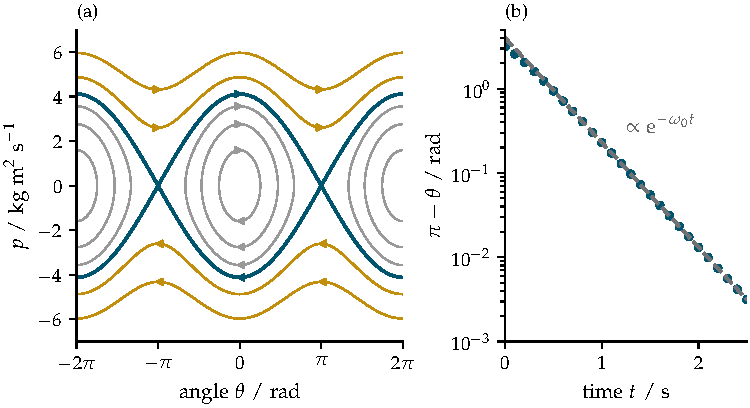
\includegraphics{ch07_hamilton/portrait}
\caption{The pendulum of \SI{0.5}{\kilogram} on a rod of
\SI{1.2}{\metre}. (a) Contours of $H$ in the phase plane, with arrowheads
showing the direction of the flow: swinging, below the upright energy
$2mgL$ (grey); the separatrix, at $2mgL$ (teal); going over the top
(ochre). (b) Started at the bottom with the momentum of the separatrix,
the angle still to go, $\pi - \theta$, from Hamilton's equations (dots),
on a logarithmic axis, against a line that falls as
$\mathrm{e}^{-\omega_0t}$ (dashed).}
\label{fig:ha-portrait}
\end{figure}

A bob given exactly this momentum at the bottom creeps towards the top
and never arrives, as \cref{sec:os-phase} said. On the separatrix the
energy is $2mgL$ at every angle, $\frac12 mL^2\dot\theta^2 + mgL(1 -
\cos\theta) = 2mgL$, so
\begin{align*}
   \dot\theta^2 &= \frac{2g}{L}\,(1 + \cos\theta)
   && \text{subtracting $mgL(1 - \cos\theta)$, dividing by
   $\tfrac12 mL^2$}\\
   &= \frac{4g}{L}\cos^2\frac{\theta}{2}
   && \text{by $\cos\theta = 2\cos^2\tfrac{\theta}{2} - 1$}\\
   \dot\theta &= 2\omega_0\cos\frac{\theta}{2}
   && \text{the root for motion towards $+\pi$,}
\end{align*}
taking the positive root because $\cos\frac{\theta}{2} > 0$ for $-\pi <
\theta < \pi$, and where the second line uses the double-angle formula of
\cref{sec:mo-trig},
$\cos\theta = \cos^2\frac{\theta}{2} - \sin^2\frac{\theta}{2}$, with
$\sin^2 = 1 - \cos^2$. Near the top, we write $\varphi = \pi - \theta$
for the angle still to go. Then $\cos\frac{\theta}{2} = \cos(\frac{\pi}{2} -
\frac{\varphi}{2}) = \sin\frac{\varphi}{2}$ (\cref{sec:mo-trig}), and $\sin\frac{\varphi}{2}
\approx \frac{\varphi}{2}$ for small $\varphi$ (\cref{sec:mo-taylor}), and $\dot\varphi = -\dot\theta$,
so
\begin{equation*}
   \dot\varphi \approx -\omega_0\,\varphi .
\end{equation*}
This is the equation of the drag of \cref{sec:ne-drag} with $\omega_0$ in
place of $\gamma$ and nothing to approach but zero, so $\varphi$ falls as
$\mathrm{e}^{-\omega_0t}$: it halves every $\ln 2/\omega_0 =
\SI{0.2425}{\second}$, however small it is, and never reaches zero.
Computed from Hamilton's equations (\cref{fig:ha-portrait}b), the bob
started at the bottom is \SI{0.229}{\radian} short of the top after
\SI{1}{\second} and \SI{0.0132}{\radian}, \ang{0.75}, short after
\SI{2}{\second}, and from then on the gap halves every
\SI{0.2425}{\second}.

\begin{keyidea}
Hamilton's equations, $\dot{q} = \partial H/\partial p$ and $\dot{p} =
-\partial H/\partial q$, move every state of phase space along a flow
that runs along the contours of $H$, so $H$ is conserved unless it
contains the time.
\end{keyidea}

\notebook{07}{launch a pendulum anywhere on its phase portrait}

\begin{selfcheck}
A ball thrown straight up has $H = p^2/(2m) + mgq$, with $q$ its height.
Write Hamilton's equations for it, and describe the contours of $H$ in
its phase plane.
\end{selfcheck}

%=============================================================================!
% 7.3  POISSON BRACKETS AND THE LIOUVILLE OPERATOR                            !
%=============================================================================!
\section{Poisson brackets and the Liouville operator}
\label{sec:ha-brackets}

Besides the coordinates, a simulation is asked for quantities computed
from the state: the energy, a momentum, the distance between two atoms,
the angle of a bond. This section finds how any such quantity changes
along the motion, and turns the answer into a series that gives the
motion from the starting state, at every time in simple cases and over a
short time in general, the form in which
Chapter~9 will build methods of computing motion.

\subsection*{The rate of change of any quantity}

Let $A(q, p)$ be any quantity computed from the state. Along a motion, by
the chain rule along a path and Hamilton's equations,
\begin{equation*}
   \frac{\dd A}{\dd t} = \frac{\partial A}{\partial q}\,\dot{q}
   + \frac{\partial A}{\partial p}\,\dot{p}
   = \frac{\partial A}{\partial q}\,\frac{\partial H}{\partial p}
   - \frac{\partial A}{\partial p}\,\frac{\partial H}{\partial q} .
\end{equation*}
The combination on the right is called the Poisson bracket of $A$ and
$H$. For any two quantities $A$ and $B$ of the state it is defined as
\begin{equation}
   \pb{A}{B} = \frac{\partial A}{\partial q}\,\frac{\partial B}{\partial p}
   - \frac{\partial A}{\partial p}\,\frac{\partial B}{\partial q} ,
   \label{eq:ha-bracket}
\end{equation}
with a sum of such terms, one for each pair $q_k$, $p_k$, when there are
several coordinates. So
\begin{equation*}
   \frac{\dd A}{\dd t} = \pb{A}{H} .
\end{equation*}
Exchanging $A$ and $B$ in \cref{eq:ha-bracket} exchanges the two
products, so $\pb{B}{A} = -\pb{A}{B}$; with $B = A$ this reads $\pb{A}{A}
= -\pb{A}{A}$, so the bracket of any quantity with itself is zero. Four cases follow at once. With $A = q$ and $B = p$,
$\partial q/\partial q = 1$, $\partial p/\partial p = 1$ and the cross
derivatives are zero, so $\pb{q}{p} = 1$. With $A = q$, $\pb{q}{H} =
\partial H/\partial p$, and with $A = p$, $\pb{p}{H} = -\partial H/
\partial q$: Hamilton's equations themselves. With $A = H$, $\pb{H}{H} =
0$: the energy is conserved. More generally, a quantity that does not
contain the time is conserved when its bracket with $H$ is zero, and only
then.
For the puck, $H = p_r^2/(2m) + p_\theta^2/(2mr^2) + U(r)$ does not contain
$\theta$. In the sum over the pairs $(r, p_r)$ and $(\theta, p_\theta)$
the only derivative of $p_\theta$ that is not zero is $\partial p_\theta/
\partial p_\theta = 1$, so $\pb{p_\theta}{H} = -\partial H/\partial\theta =
0$, and the
angular momentum $p_\theta$ is conserved; \cref{ex:ha-lz} finds the same in
Cartesian coordinates.

\begin{bridge}
Dirac found that the equations of quantum mechanics follow from the
classical ones when the Poisson bracket $\pb{A}{B}$ is replaced by the
commutator $(AB - BA)/(\mathrm{i}\hbar)$ of the corresponding
operators\cite{Dirac1925}. Then $\pb{q}{p} = 1$ becomes $qp - pq =
\mathrm{i}\hbar$, and $\dd A/\dd t = \pb{A}{H}$ becomes Heisenberg's
equation of motion. A quantity that commutes with the Hamiltonian is
conserved in both.
\end{bridge}

\subsection*{The Liouville operator}

The bracket with $H$ is an instruction that turns any quantity into its
rate of change. Writing it as $\Liou$,
\begin{equation*}
   \Liou A = \pb{A}{H}
   = \dot{q}\,\frac{\partial A}{\partial q}
   + \dot{p}\,\frac{\partial A}{\partial p} ,
\end{equation*}
where $\dot{q} = \partial H/\partial p$ and $\dot{p} = -\partial H/
\partial q$ are written in terms of $q$ and $p$. An instruction of this
kind, which acts on a function to give another, is called an operator,
as $\dd/\dd x$ is the operator that gives a derivative; $\Liou$ is the
Liouville operator. The result $\Liou A$ is again a quantity of the
state, so its own rate of change is $\Liou(\Liou A)$, written $\Liou^2A$,
and this is the second derivative of $A$ along the motion. Repeating,
the $n$th derivative of $A$ along the motion is $\Liou^nA$. The Taylor
series of \cref{sec:mo-taylor}, taken about the start of the motion,
then gives
\begin{equation}
      A\bigl(q(t), p(t)\bigr) = A + t\,\Liou A + \frac{t^2}{2!}\,\Liou^2A
   + \frac{t^3}{3!}\,\Liou^3A + \dotsb
   = \sum_{n=0}^{\infty}\frac{t^n}{n!}\,\Liou^nA ,
   \label{eq:ha-series}
\end{equation}
with every term on the right computed at the starting state $(q_0, p_0)$
and $\Liou^0A = A$. For the functions of \cref{sec:mo-taylor} the infinite
series converges at every $t$; in general only the series stopped after a
few terms can be relied on, and only over a short time.

For a ball thrown straight up, $H = p^2/(2m) + mgq$, so $\dot{q} = p/m$,
$\dot{p} = -mg$ and $\Liou = (p/m)\,\partial/\partial q - mg\,\partial/
\partial p$. Applying it to $q$ repeatedly,
\begin{equation*}
   \Liou q = \frac{p}{m} , \qquad
   \Liou^2q = \Liou\frac{p}{m} = -mg\times\frac{1}{m} = -g , \qquad
   \Liou^3q = \Liou(-g) = 0 ,
\end{equation*}
since $-g$ contains neither $q$ nor $p$. Every later term is zero too, and
\cref{eq:ha-series} gives $q(t) = q_0 + p_0t/m - \frac12 gt^2$, the ball
of \cref{sec:mo-velocity}.

For the block on a spring, $\dot{q} = p/m$, $\dot{p} = -kq$ and $\Liou =
(p/m)\,\partial/\partial q - kq\,\partial/\partial p$. With $\omega^2 =
k/m$,
\begin{align*}
   \Liou q &= \frac{p}{m} ,
   & \Liou^2q &= \Liou\frac{p}{m} = -\frac{kq}{m} = -\omega^2q ,\\
   \Liou^3q &= -\omega^2\,\Liou q = -\omega^2\,\frac{p}{m} ,
   & \Liou^4q &= -\omega^2\,\Liou^2q = \omega^4q ,
\end{align*}
since $\Liou$ of a constant times a quantity is the constant times $\Liou$
of the quantity. The pattern repeats every two steps, each pair bringing
a factor $-\omega^2$. Term by term, \cref{eq:ha-series} gives
\begin{equation*}
   q(t) = q_0 + t\,\frac{p_0}{m} - \frac{t^2}{2!}\,\omega^2q_0
   - \frac{t^3}{3!}\,\omega^2\,\frac{p_0}{m} + \frac{t^4}{4!}\,\omega^4q_0
   + \dotsb .
\end{equation*}
Gathering the terms in $q_0$ and in $p_0$ separately, and writing each
power of $t$ with the matching power of $\omega$, which for the terms in
$p_0$ means writing $p_0/m = \bigl(p_0/(m\omega)\bigr)\,\omega$,
\begin{align*}
   q(t) &= q_0\Bigl(1 - \frac{(\omega t)^2}{2!} + \frac{(\omega t)^4}{4!}
   - \dotsb\Bigr)
   + \frac{p_0}{m\omega}\Bigl(\omega t - \frac{(\omega t)^3}{3!}
   + \dotsb\Bigr)\\
   &= q_0\cos\omega t + \frac{p_0}{m\omega}\sin\omega t ,
\end{align*}
by the series of \cref{eq:mo-sin-series}. With $p_0 = mv_0$ this is
\cref{eq:ne-spring-solution}. For the pendulum the terms $\Liou^n\theta$
grow more complicated, and Notebook~07 shows that a few of them follow
the motion well over a short time but not over a long one. Chapter~9 writes
the series \cref{eq:ha-series} as an exponential of $t\Liou$ and splits
$\Liou$ into a part that moves only the positions and a part that moves
only the momenta, each of which can be followed exactly; that splitting is
how the standard method of molecular dynamics is derived.

\begin{keyidea}
Any quantity of the state changes at the rate $\dd A/\dd t = \pb{A}{H} =
\Liou A$, and is conserved when its Poisson bracket with $H$ is zero.
Repeating the Liouville operator $\Liou$ gives every derivative of $A$, and
the Taylor series $\sum_n(t^n/n!)\,\Liou^nA$ gives its value at later
times from the starting state: at every time for the ball and the spring,
over a short time in general.
\end{keyidea}

\notebook{07}{the series of the Liouville operator, term by term}

\begin{selfcheck}
For the block on a spring, find $\Liou(qp)$. At which states is the
product $qp$ momentarily not changing?
\end{selfcheck}

%=============================================================================!
% 7.4  LIOUVILLE'S THEOREM                                                    !
%=============================================================================!
\section{Liouville's theorem}
\label{sec:ha-liouville}

A drop of ink in a shallow, slow stream, whose water moves alike at every
depth, is carried downstream, stretched and folded by the current; the
water cannot be squeezed, and none rises from below or sinks, so the patch
of ink keeps its area while its shape changes. The Hamiltonian
flow does the same to a patch of states. We start many copies of
the pendulum from slightly different states, filling a small region of
the phase plane, a blob, and let each move by Hamilton's equations. This
section shows that the blob keeps its area, whatever the system, and that
drag makes it shrink.

\Cref{fig:ha-blob}(a) follows such a blob of pendulums: an ellipse of
starting states centred on \SI{1.6}{\radian} at rest, reaching
\SI{0.4}{\radian} either side in angle and
\SI{0.8}{\kilogram\metre\squared\per\second} either way in momentum, a
circle of radius 1 stretched by 0.4 along one axis and 0.8 along the
other. Swings of different
size take different times (\cref{sec:os-anharmonic}), so the blob is
sheared into a curved streak; yet its area, $\pi\times0.4\times0.8 = \SI{1.00531}{\joule\second}$,
is the same at every time drawn, to within 2.6 parts in $10^7$, the error
of drawing its edge with 6000 points. An area in this plane is an angle
times an angular momentum, and has the unit of the action of
\cref{sec:la-action}.

\begin{figure}[htb]
\centering
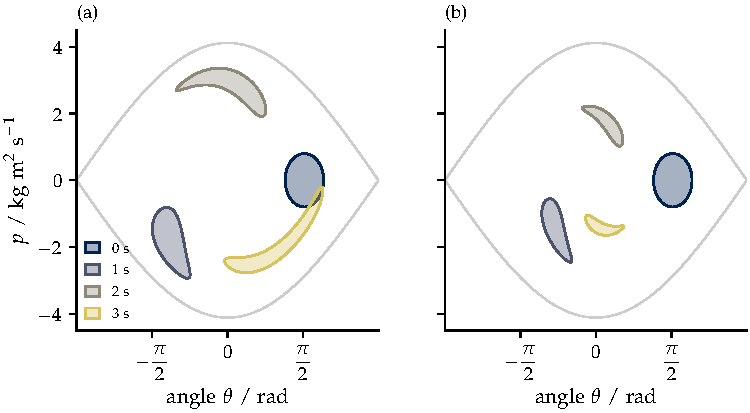
\includegraphics{ch07_hamilton/blob}
\caption{A blob of states of the pendulum of \cref{fig:ha-portrait},
centred on $\theta = \SI{1.6}{\radian}$ at rest, carried by the flow and
drawn at the times given, inside the separatrix (grey). (a) Without drag:
sheared, with its area unchanged. (b) With the drag rate $\gamma =
\SI{0.5}{\per\second}$: shrinking towards the state of rest at the
bottom.}
\label{fig:ha-blob}
\end{figure}

\subsection*{Why the area is kept}

We write the velocity of the flow at the point $(q, p)$ as $(u, w)$, with
$u = \dot{q}$ and $w = \dot{p}$. Each short piece of the edge of the
blob, of length $\Delta s$, moves with the flow, and in a short time
$\tau$ it sweeps out a thin strip. Only the part of the velocity at
right angles to the piece sweeps area, so if $\vb{n}$ is the arrow of
length one at right angles to the piece, pointing out of the blob, the
strip has the area $(u, w)\cdot\vb{n}\,\Delta s\,\tau$, counted
positive when the edge moves outwards. Adding the strips around the whole
edge, the area $\mathcal{A}$ of the blob changes at the rate
\begin{equation*}
   \frac{\dd\mathcal{A}}{\dd t} = \oint (u, w)\cdot\vb{n}\,\dd s ,
\end{equation*}
the flow out through the edge. Going round the edge anticlockwise, a
piece $(\Delta q, \Delta p)$ has the blob on its left, and turning it a
right angle clockwise gives $(\Delta p, -\Delta q)$, which points out of
the blob and has the length $\Delta s$; so $\vb{n}\,\Delta s = (\Delta
p, -\Delta q)$, and
\begin{equation*}
   \frac{\dd\mathcal{A}}{\dd t} = \oint\bigl(u\,\dd p - w\,\dd q\bigr) .
\end{equation*}
Green's theorem (\cref{sec:en-curl}) turns a loop integral into an
integral over the area inside: for any smooth $(F_q, F_p)$, $\oint(F_q\,
\dd q + F_p\,\dd p) = \iint(\partial F_p/\partial q - \partial F_q/\partial
p)\,\dd A$, around the loop anticlockwise. With $F_q = -w$ and $F_p = u$,
\begin{equation}
   \frac{\dd\mathcal{A}}{\dd t} = \iint\Bigl(\frac{\partial u}{\partial q}
   + \frac{\partial w}{\partial p}\Bigr)\dd A .
   \label{eq:ha-area-rate}
\end{equation}
The sum in the large brackets is called the divergence of the flow: by
\cref{eq:ha-area-rate}, applied to a blob so small that the sum hardly
changes across it, it is the rate at which the blob's area grows, divided
by that area. For the Hamiltonian
flow, $u = \partial H/\partial p$ and $w = -\partial H/\partial q$, so
\begin{equation*}
   \frac{\partial u}{\partial q} + \frac{\partial w}{\partial p}
   = \frac{\partial^2H}{\partial q\,\partial p}
   - \frac{\partial^2H}{\partial p\,\partial q} = 0 ,
\end{equation*}
because the two mixed partial derivatives of a smooth function are equal
(\cref{sec:en-curl}). The integrand is zero everywhere, so $\dd\mathcal{A}
/\dd t = 0$: the Hamiltonian flow keeps the area of every region it
carries. This is Liouville's theorem.

With the drag of \cref{sec:os-damped}, $\dot{p} = -\partial H/\partial q -
\gamma p$, so $w$ gains the term $-\gamma p$, and $\partial w/\partial p$
gains $-\gamma$. The divergence is then $-\gamma$ everywhere, and
\cref{eq:ha-area-rate} gives $\dd\mathcal{A}/\dd t = -\gamma\mathcal{A}$,
the equation of \cref{sec:ne-drag}, so
\begin{equation*}
   \mathcal{A}(t) = \mathcal{A}_0\,\mathrm{e}^{-\gamma t} .
\end{equation*}
With $\gamma = \SI{0.5}{\per\second}$, the blob of \cref{fig:ha-blob}(b)
keeps 0.60653, 0.36788 and 0.22313 of its area after 1, 2 and
\SI{3}{\second}, the values of $\mathrm{e}^{-\gamma t}$ to the five
figures printed. Every state ends at rest at the bottom: the drag erases
the differences between starting states, which a Hamiltonian flow never
does.

\subsection*{The stretching of a small square}

Liouville's theorem can also be read off a single state and its close
neighbours, which is the form Chapter~9 uses for methods that move in
steps.

\begin{toolbox}[The Jacobian determinant]
The flow over a time $t$ carries each starting state $(q_0, p_0)$ to the
state $(q, p)$ reached at time $t$, so $q$ and $p$ are functions of $q_0$
and $p_0$. We take a small square of starting states with one corner at
$(q_0, p_0)$ and sides of length $\varepsilon$ along the two axes
(\cref{fig:ha-square}). By the Taylor series to first order, the corner
at $(q_0 + \varepsilon, p_0)$ goes to $(q, p) + \varepsilon\,\vb{a}$, with
$\vb{a} = (\partial q/\partial q_0, \partial p/\partial q_0)$, and the
corner at $(q_0, p_0 + \varepsilon)$ goes to $(q, p) + \varepsilon\,
\vb{b}$, with $\vb{b} = (\partial q/\partial p_0, \partial p/\partial
p_0)$. The far corner $(q_0 + \varepsilon, p_0 +
\varepsilon)$ is a step $\varepsilon$ in both variables, and the
first-order rule $\Delta h \approx (\partial h/\partial x)\,\Delta x +
(\partial h/\partial y)\,\Delta y$ of \cref{sec:en-gradient}, applied to
$q$ and to $p$, takes it to $(q, p) + \varepsilon\vb{a} + \varepsilon
\vb{b}$. To first order, then, the square becomes the parallelogram on the
arrows $\varepsilon\vb{a}$ and $\varepsilon\vb{b}$. The area of the
parallelogram on $\vb{a} = (a_1, a_2)$ and $\vb{b} = (b_1, b_2)$ is the
length of their cross product (\cref{sec:ro-cross}); with third
components zero, the cross product has only the third component $a_1b_2 -
a_2b_1$, so the area is $\lvert a_1b_2 - a_2b_1\rvert$. The four
derivatives form the Jacobian matrix of the flow,
\begin{equation*}
   \vb{J} = \begin{pmatrix}
      \partial q/\partial q_0 & \partial q/\partial p_0\\
      \partial p/\partial q_0 & \partial p/\partial p_0
   \end{pmatrix} ,
\end{equation*}
whose columns are $\vb{a}$ and $\vb{b}$, and the number $a_1b_2 - a_2b_1$
made from a $2\times2$ matrix in this way, the product of the diagonal
entries minus the product of the other two, is its determinant, $\det
\vb{J}$. The square of area $\varepsilon^2$ therefore becomes a
parallelogram of area $\lvert\det\vb{J}\rvert\,\varepsilon^2$: the
determinant is the factor by which the flow stretches small areas. For a
body in free flight, $q = q_0 + p_0t/m$ and $p = p_0$, so
\begin{equation*}
   \vb{J} = \begin{pmatrix} 1 & t/m\\ 0 & 1 \end{pmatrix} ,
   \qquad \det\vb{J} = 1\times1 - \frac{t}{m}\times0 = 1 ,
\end{equation*}
a shear that tilts the square without changing its area
(\cref{ex:ha-shear}). For a map of $n$ variables, the $n\times n$
Jacobian matrix has a determinant too, the factor by which the map
stretches small volumes in $n$ dimensions; its definition for larger
matrices, and this property, are standard results of linear algebra that
we take on trust.
\end{toolbox}

\begin{figure}[htb]
\centering
\begin{tikzpicture}[line cap=round, line join=round, scale=1.15,
   arr/.style={-{Stealth[length=5pt]}, line width=0.8pt}]
   \fill[black!8] (0,0) rectangle (1.6,1.6);
   \draw[line width=0.8pt] (0,0) rectangle (1.6,1.6);
   \draw[arr, accent] (0,0) -- (1.6,0) node[midway, below=2pt]
      {\small $\varepsilon$ along $q_0$};
   \draw[arr, accent] (0,0) -- (0,1.6) node[midway, left]
      {\small $\varepsilon$ along $p_0$};
   \fill (0,0) circle (1.2pt) node[left=3pt] {\small $(q_0, p_0)$};
   \draw[-{Stealth[length=6pt]}, line width=0.6pt, black!50]
      (2.2,0.9) to[bend left=20] node[midway, above] {\small flow} (3.8,0.9);
   \begin{scope}[shift={(4.6,0.0)}]
            \fill[black!8] (0,0) -- (1.8,0.55) -- (2.55,2.2) -- (0.75,1.65) -- cycle;
      \draw[line width=0.8pt] (0,0) -- (1.8,0.55) -- (2.55,2.2) -- (0.75,1.65)
         -- cycle;
      \draw[arr, accent] (0,0) -- (1.8,0.55) node[midway, below right]
         {\small $\varepsilon\vb{a}$};
            \draw[arr, accent] (0,0) -- (0.75,1.65) node[midway, left]
         {\small $\varepsilon\vb{b}$};
      \fill (0,0) circle (1.2pt) node[below left] {\small $(q, p)$};
   \end{scope}
\end{tikzpicture}
\caption{The flow over a time $t$ carries a small square of starting
states into a parallelogram on the arrows $\varepsilon\vb{a}$ and
$\varepsilon\vb{b}$, the columns of the Jacobian matrix times the side
$\varepsilon$; its area is $\lvert\det\vb{J}\rvert$ times that of the
square.}
\label{fig:ha-square}
\end{figure}

Since the Hamiltonian flow keeps the area of every region, a small square
keeps its area $\varepsilon^2$, while the toolbox gives $\lvert\det\vb{J}
\rvert\,\varepsilon^2$ with an error that shrinks faster than
$\varepsilon^2$; letting $\varepsilon$ shrink, $\lvert\det\vb{J}\rvert =
1$. At $t = 0$ the map does nothing and $\det\vb{J} = 1\times1 - 0\times0
= 1$, and $\det\vb{J}$ changes smoothly with $t$, so it cannot jump to
$-1$: $\det\vb{J} = 1$ at every time. With drag, the same reasoning gives
$\det\vb{J} = \mathrm{e}^{-\gamma t}$. Computed with
\texttt{flow\_jacobian}, which follows four copies started a small step
either side of the state along each axis and takes central differences
(\cref{sec:mo-atoms}) of where they arrive, the Jacobian of the pendulum's flow from
$(\theta, p) = (\SI{1}{\radian}, \SI{0.5}{\kilogram\metre\squared\per
\second})$ over \SI{2.5}{\second} has a determinant that differs from 1 by
about
$10^{-10}$, although the map is far from doing nothing: its entries are
1.057 and 0.213 in the first row and 1.157 and 1.179 in the second;
rounded, they give $1.057\times1.179 - 0.213\times1.157 = 0.9998$, which is
1 to the accuracy of the rounding.

For $N$ atoms the same holds in the $6N$ dimensions of phase space. The
divergence of the flow is the sum, over all $6N$ coordinates, of the
derivative of each coordinate's rate with respect to that coordinate,
$\sum_k(\partial\dot{q}_k/\partial q_k + \partial\dot{p}_k/\partial p_k)$;
for Hamilton's equations it is $\sum_k(\partial^2H/\partial q_k\partial
p_k - \partial^2H/\partial p_k\partial q_k)$, zero term by term, and the form of
Green's theorem in many dimensions, the divergence
theorem\cite{Tuckerman2023}, then shows that every region of phase space
keeps its volume and $\det\vb{J} = 1$. A cloud of states can be stretched and folded by
the flow but never compressed. In particular, the number of copies in a
small region that moves with the flow does not change, and neither does
its volume, so the density of copies seen by an observer moving with any
one state stays the same. Since each state also keeps its energy, a cloud
whose density, the number of copies per unit volume, is a function
$f(H)$ of the energy alone does not change at all: the copies now at a
state $\Gamma$ came from a state of the same energy, where the density was
$f\bigl(H(\Gamma)\bigr)$, and have kept that density. Chapter~12 builds statistical mechanics
on such clouds.

\begin{keyidea}
The Hamiltonian flow has zero divergence, because the mixed partial
derivatives of $H$ are equal, so it keeps the area, in many dimensions the
volume, of every region of phase space it carries: the Jacobian
determinant of the flow is 1. Drag at the rate $\gamma$ shrinks areas as
$\mathrm{e}^{-\gamma t}$.
\end{keyidea}

\notebook{07}{watch a blob of states flow, with and without drag}

\begin{selfcheck}
A blob of states of the pendulum with drag at $\gamma =
\SI{0.5}{\per\second}$ has an area of \SI{1}{\joule\second}. What is its
area \SI{4}{\second} later?
\end{selfcheck}

%=============================================================================!
% 7.5  SYMMETRIES AND CONSERVED QUANTITIES                                    !
%=============================================================================!
\section{Symmetries and conserved quantities}
\label{sec:ha-noether}

Two carts joined by a spring on a straight track (\cref{sec:ne-bodies})
have an energy that depends only on the distance between them, so sliding
both along the track by the same amount changes nothing. Chapter~2 found
that their total momentum is conserved, because the spring pushes them
equally and oppositely. This section shows that the conservation follows
from the symmetry itself, that the energy is unchanged by the shift,
whatever the forces are like, and that the same holds for turning and for
the passing of time.

\subsection*{Moving everything at once}

Let the potential energy of $N$ atoms be unchanged when every atom is
moved by the same displacement $\vb{c}$:
\begin{equation*}
   U(\vb{r}_1 + \vb{c}, \dots, \vb{r}_N + \vb{c})
   = U(\vb{r}_1, \dots, \vb{r}_N)
   \qquad\text{for every } \vb{c} .
\end{equation*}
With $\vb{c} = (c, 0, 0)$ along $x$, we differentiate both sides with
respect to $c$. On the left, each $x_i$ is replaced by $x_i + c$, which
changes at the rate 1 as $c$ grows, so the general chain rule
(\cref{sec:ha-equations}) gives one term for each atom; the right does
not contain $c$. At $c = 0$,
\begin{equation*}
   \sum_{i=1}^{N}\frac{\partial U}{\partial x_i} = 0 ,
   \qquad\text{so}\qquad
   \sum_{i=1}^{N}F_{i,x} = 0 ,
\end{equation*}
and the same for $y$ and $z$: the forces on the atoms add to zero. By
Hamilton's equations $\dot{\vb{p}}_i = \vb{F}_i$, so the total momentum
$\vb{P} = \sum_i\vb{p}_i$ changes at the rate $\sum_i\vb{F}_i = 0$ and is
conserved. Nothing here assumed that the forces act between pairs. The
atoms of \cref{fig:ha-noether}(a) have an energy that depends only on the
angle at the middle one, $U = \frac12 k_\theta(\theta - \theta_0)^2$,
a simple model of the bending of a molecule. The forces,
0.890, 1.430 and \SI{0.685}{\electronvolt\per\angstrom}, are not along the
lines that join the atoms (the force on atom~1 is at right angles to its
bond), yet they add to zero to within $5\times10^{-10}$
\si{\electronvolt\per\angstrom}, the error of the central differences
that computed them. This is the reason promised in \cref{sec:ne-atoms}.

\subsection*{Turning everything at once}

Now let $U$ be unchanged when the whole group is turned by any angle
about any axis through the origin. Turning at the angular velocity
$\vb{n}$, an arrow of length one along the axis, that is at one radian per
unit of time, for a time $\alpha$ turns the group by the angle $\alpha$,
and to first order each atom moves by its velocity times $\alpha$,
$\alpha\,\vb{n}\times\vb{r}_i$ (\cref{sec:ro-rigid}). Differentiating $U$ with respect to
$\alpha$ at $\alpha = 0$ by the general chain rule, one term for each
coordinate of each atom,
\begin{align*}
   0 &= \sum_{i=1}^{N}\grad_iU\cdot(\vb{n}\times\vb{r}_i)
   && \text{since $U$ does not change}\\
   &= \sum_{i=1}^{N}\vb{n}\cdot(\vb{r}_i\times\grad_iU)
   && \text{moving the three vectors round (\cref{sec:ro-tensor})}\\
   &= -\vb{n}\cdot\sum_{i=1}^{N}\vb{r}_i\times\vb{F}_i
   = -\vb{n}\cdot\vb{G}
   && \text{with $\vb{F}_i = -\grad_iU$.}
\end{align*}
This holds for every axis $\vb{n}$, so every component of the total
torque $\vb{G}$ is zero. The angular momentum $\vb{L} = \sum_i\vb{r}_i
\times\vb{p}_i$ changes, by the product rule, at the rate
\begin{equation*}
   \frac{\dd\vb{L}}{\dd t} = \sum_{i=1}^{N}\Bigl(\frac{\vb{p}_i}{m_i}
   \times\vb{p}_i + \vb{r}_i\times\vb{F}_i\Bigr) = \vb{G} = 0 ,
\end{equation*}
since the cross product of an arrow with itself is zero; so $\vb{L}$ is
conserved. For the three atoms of \cref{fig:ha-noether}(a) the torque is
below $2\times10^{-9}$ \si{\electronvolt}, about the origin and about the
point $(3, 2)$~\si{\angstrom}, again the error of the differences. This is the result
promised in \cref{sec:ro-system} for forces that cannot be split into
pairs.

\begin{figure}[htb]
\centering
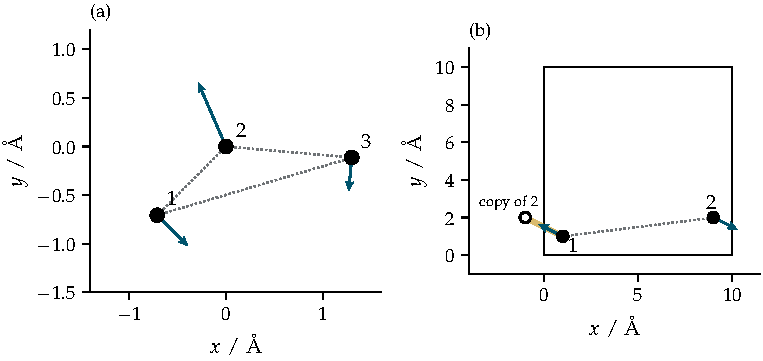
\includegraphics{ch07_hamilton/noether}
\caption{(a) Three atoms whose energy depends only on the angle at atom~2,
$\frac12 k_\theta(\theta - \theta_0)^2$ with $k_\theta =
\SI{2}{\electronvolt\per\radian\squared}$ and $\theta_0 = \ang{104.5}$,
held at \ang{130} with bonds of 1.0 and \SI{1.3}{\angstrom}. The forces
(arrows, \SI{0.5}{\angstrom} per \si{\electronvolt\per\angstrom}) are not
along the lines joining the atoms (dotted), yet add to zero with no
torque. (b) Two atoms in a box \SI{10}{\angstrom} wide repeated in every
direction, joined by a spring to the nearest copy of each other (ochre);
the forces (\SI{6}{\angstrom} per \si{\electronvolt\per\angstrom}) add to
zero but are not along the line joining the atoms in the box (dotted), so
they exert a torque.}
\label{fig:ha-noether}
\end{figure}

\subsection*{Noether's theorem}

Both results, and the conservation of a momentum whose coordinate is
missing from $\Lag$ (\cref{sec:la-polar}), are cases of one theorem,
proved most directly from the Lagrangian. Suppose that $\Lag$ does not
change, to first order in a small number $\alpha$, when every coordinate
is changed by $\alpha s_k(q)$, with $s_k$ any functions of the
coordinates, and every rate by the matching $\alpha\,\dd s_k/\dd t$, the
rate of $q_k + \alpha s_k$ being $\dot{q}_k + \alpha\,\dd s_k/\dd t$. Then,
by the chain rule,
\begin{align*}
   0 &= \sum_k\Bigl(\frac{\partial\Lag}{\partial q_k}\,s_k
   + \frac{\partial\Lag}{\partial\dot{q}_k}\,\frac{\dd s_k}{\dd t}\Bigr)
   && \text{the change of $\Lag$ per unit of $\alpha$}\\
   &= \sum_k\Bigl(\dot{p}_k\,s_k + p_k\,\frac{\dd s_k}{\dd t}\Bigr)
   && \text{by \cref{eq:la-euler} and $p_k = \partial\Lag/\partial
   \dot{q}_k$}\\
   &= \frac{\dd}{\dd t}\sum_k p_k\,s_k
   && \text{by the product rule,}
\end{align*}
so $\sum_k p_ks_k$ is conserved. Moving every atom along $x$ has $s = 1$
for every $x_i$ and 0 for the other coordinates, and leaves the kinetic
energy unchanged, so $\sum_ip_{i,x}$ is conserved. Turning about
$\vb{n}$ has the change $\vb{n}\times\vb{r}_i$ for atom $i$, and leaves
$\frac12 m_i\lvert\dot{\vb{r}}_i\rvert^2$ unchanged, since the rate
changes by $\alpha\,\vb{n}\times\dot{\vb{r}}_i$, at right angles to
$\dot{\vb{r}}_i$: $\lvert\dot{\vb{r}}_i + \alpha\,\vb{n}\times\dot{\vb{r}}_i
\rvert^2 = \lvert\dot{\vb{r}}_i\rvert^2 + 2\alpha\,\dot{\vb{r}}_i\cdot
(\vb{n}\times\dot{\vb{r}}_i) + \order{\alpha^2}$, and the middle term is
zero (\cref{sec:ro-cross}). So $\sum_i\vb{p}_i\cdot(\vb{n}\times\vb{r}_i)
= \vb{n}\cdot\vb{L}$ is conserved, by the triple product again. A
coordinate missing from $\Lag$ has $s = 1$ for itself and 0 for the
others, and its own momentum is conserved. The passing of time is the
remaining symmetry, though not of this form: \cref{sec:ha-equations}
showed directly that a Hamiltonian that does not contain $t$ is
conserved. Each symmetry of $\Lag$ under a change that can be made as
small as we like, and the passing of time for $H$, comes with a conserved
quantity: this is Noether's theorem, named after Emmy Noether.

\subsection*{A box repeated in every direction}

Most simulations follow the atoms in a box repeated periodically in every
direction (Chapter~10), and each atom feels the nearest copies of the
others. Moving every atom by the same displacement moves every copy too,
and changes nothing, so the forces still add to zero and the total
momentum is conserved. Turning the atoms while the box and the lattice of
its copies stay fixed is not a symmetry. In \cref{fig:ha-noether}(b) two
atoms at $(1, 1)$ and $(9, 2)$~\si{\angstrom} in a box \SI{10}{\angstrom}
wide are joined by a spring of \SI{1}{\electronvolt\per\angstrom\squared}
and natural length \SI{2}{\angstrom} to the nearest copy of each other.
The nearest copy of atom~2, one box width to the left, is at $(9 - 10,
2) = (-1, 2)$~\si{\angstrom}, at the
separation $(-2, 1)$ and the distance $\sqrt5 = \SI{2.2361}{\angstrom}$, so
the spring is stretched by \SI{0.2361}{\angstrom} and pulls atom~1 towards
that copy with $\vb{F}_1 = k\times0.2361\times(-2, 1)/\sqrt5 = (-0.2111,
0.1056)$
\si{\electronvolt\per\angstrom}; atom~2 feels the opposite force, from the
copy of atom~1. The forces add to zero, and moving both atoms by any
displacement leaves the energy at \SI{0.027864}{\electronvolt}. They act along
the line from atom~1 to the copy, at an angle to the line joining the two
atoms in the box, and their torque about the origin is
\begin{equation*}
   G_z = (x_1 - x_2)\,F_{1,y} - (y_1 - y_2)\,F_{1,x}
   = (-8)(0.1056) - (-1)(-0.2111) = \SI{-1.056}{\electronvolt} ,
\end{equation*}
using $\vb{F}_2 = -\vb{F}_1$ in $G_z = \sum_i(x_iF_{i,y} - y_iF_{i,x})$.
Turning both atoms about the origin changes the energy at the rate
$\SI{1.056}{\electronvolt}$ per radian, so the angular momentum of the
atoms in the box is not conserved, and \cref{sec:ro-remove} removed only
the drift of a periodic system.

A learned model of the forces keeps these conservation laws when its
forces are the slopes of an energy with the same symmetries. A learned
model of the motion predicts the next state without Hamilton's equations,
so the theorem does not cover it even when it respects the symmetries,
which is why TrajCast corrects its predicted momenta, as the planned
Chapter~28 will discuss.

\begin{keyidea}
Every symmetry of the Lagrangian under a change that can be made as small
as we like gives a conserved quantity (Noether's theorem), and so does
the passing of time: unchanged by
moving everything, the total momentum; by turning everything, the angular
momentum; by the passing of time, the energy. No assumption about pairs of
forces is needed.
\end{keyidea}

\notebook{07}{forces of a bending molecule and of atoms in a periodic box}

\begin{selfcheck}
A fixed flat wall at $x = 0$ that repels atoms is added to a periodic
box. Which components of the total momentum are still conserved?
\end{selfcheck}

%=============================================================================!
% 7.6  RUNNING THE MOTION BACKWARDS                                           !
%=============================================================================!
\section{Running the motion backwards}
\label{sec:ha-reversal}

A film of a swinging pendulum looks as natural when it is run
backwards; a film of a book sliding to rest across a table does not,
because books are never seen to gather speed from a table that has cooled
a little. This section shows that the difference lies in the drag, and
that motion under a time-independent Hamiltonian can be reversed when
reversing every momentum leaves that Hamiltonian unchanged.

\subsection*{The reversed motion}

Let $q(t)$ and $p(t)$ be a motion. The reversed motion visits the same
positions in the opposite order, with every momentum reversed:
\begin{equation*}
   Q(t) = q(-t) , \qquad P(t) = -p(-t) .
\end{equation*}
Suppose that $H$ does not contain $t$ and that $H(q, -p) = H(q, p)$, as
it is whenever $K$ depends on the momenta through their squares. Differentiating this identity with respect
to $p$, by the chain rule on the left, gives $-(\partial H/\partial p)(q,
-p) = (\partial H/\partial p)(q, p)$, so reversing the momentum reverses
the sign of $\partial H/\partial p$; differentiating it with respect to
$q$ gives $(\partial H/\partial q)(q, -p) = (\partial H/\partial q)(q,
p)$, so reversing the momentum leaves $\partial H/\partial q$ unchanged.
Then, by the chain rule with the inner function $-t$, whose rate is $-1$,
and Hamilton's equations for the original motion at the time $-t$,
\begin{align*}
   \frac{\dd Q}{\dd t} &= -\dot{q}(-t)
   = -\frac{\partial H}{\partial p}\bigl(q(-t), p(-t)\bigr)
   = \frac{\partial H}{\partial p}(Q, P) ,\\
   \frac{\dd P}{\dd t} &= \dot{p}(-t)
   = -\frac{\partial H}{\partial q}\bigl(q(-t), p(-t)\bigr)
   = -\frac{\partial H}{\partial q}(Q, P) ,
\end{align*}
where the last step of each line uses $Q = q(-t)$, $P = -p(-t)$ and the two
results just found. The reversed motion obeys Hamilton's equations too.
Since $H$ does not contain $t$, shifting the time changes nothing in these
equations, so $q(\tau - t)$, $-p(\tau - t)$ obeys them as well. It starts
at $\bigl(q(\tau), -p(\tau)\bigr)$, and a state fixes the motion that
follows it (\cref{sec:ne-equations}), so if a motion is stopped at a time
$\tau$, every momentum is reversed, and the motion is followed for another time $\tau$, the system retraces
its path and arrives where it started, with its starting momenta
reversed.

\Cref{fig:ha-reversal}(a) shows this for a puck of \SI{0.2}{\kilogram}
on smooth ice, held near a point by springs that are stiffer north--south
(\SI{5}{\newton\per\metre}) than east--west (\SI{2}{\newton\per\metre}),
so that it traces a looping path. Followed for \SI{4}{\second}, reversed
and followed for another \SI{4}{\second}, it returns to within $3\times
10^{-14}$~\si{\metre} of its start, with the momentum
$(-0.02, -0.10)$~\si{\kilogram\metre\per\second}, the reverse of the one it
started with.

\begin{figure}[htb]
\centering
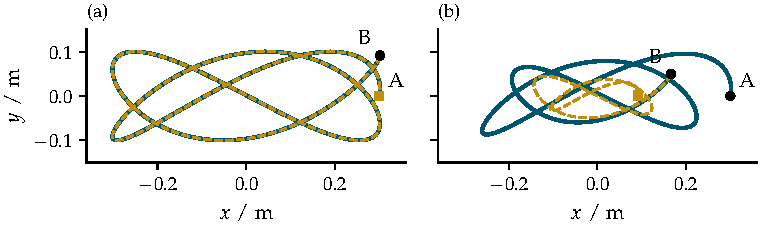
\includegraphics{ch07_hamilton/reversal}
\caption{A puck of \SI{0.2}{\kilogram} on springs of 2 (east--west) and
\SI{5}{\newton\per\metre} (north--south), started at A with the velocity
$(0.1, 0.5)$~\si{\metre\per\second}, followed for \SI{4}{\second} to B
(teal), then with every momentum reversed for another \SI{4}{\second}
(ochre, dashed), ending at the square. (a) Without drag it retraces its
path to A. (b) With drag at $\gamma = \SI{0.3}{\per\second}$ it does
not.}
\label{fig:ha-reversal}
\end{figure}

\subsection*{Drag breaks the symmetry}

With drag, $\dot{p} = -\partial H/\partial q - \gamma p$. Repeating the
second line above, the reversed motion has $\dd P/\dd t = \dot{p}(-t) =
-\partial H/\partial q - \gamma p(-t) = -\partial H/\partial q + \gamma P$:
it would need a force that pushes the puck along its motion, in place of
one that resists it, and the dragged equations do not supply one.
\Cref{fig:ha-reversal}(b) shows the result: after the reversal the puck
keeps losing energy and ends \SI{0.21}{\metre} from its start. Sliding friction,
like drag, always opposes the motion, so the reversed slide would need it
to push instead; it is what makes the book's slide irreversible, and the
motion of atoms under forces from a potential has no such term.

Chapter~9 asks the same of a method of computing motion: one step
forwards, a reversal of the momenta and one more step should bring the
system back to where it began, as the exact motion does.

\begin{keyidea}
When $H$ is time-independent and unchanged by reversing the momenta, the reversed motion $q(-t)$,
$-p(-t)$ obeys Hamilton's equations, so reversing every momentum makes a
system retrace its path. Drag breaks this.
\end{keyidea}

\begin{selfcheck}
A ball thrown straight up at \SI{12}{\metre\per\second} reaches its highest
point after \SI{1.224}{\second}. Using time reversal, and without solving
any equation, say when and how fast it comes back to the hand.
\end{selfcheck}

%=============================================================================!
% 7.7  STEPS THAT KEEP AREA                                                   !
%=============================================================================!
\section{Steps that keep area}
\label{sec:ha-symplectic}

A computer follows a motion in steps. A method of computing motion takes
the state $(q, p)$ at one instant and returns the state $(q', p')$ a time
$\dt$ later, so it is a map of the phase plane into itself, a step map,
and like the flow it has a Jacobian determinant. The exact flow over $\dt$
keeps both the energy and areas. This section shows, for the spring and
the two simplest methods, that a step map which inflates areas makes the
energy grow without limit, while the area-preserving method holds the energy within a band for
the stable step used here.

\subsection*{The forward Euler method}

The simplest step takes the rates at the start of the step as if they held throughout it, so that the change over the step is the
rate times $\dt$, the secant of \cref{sec:mo-velocity} read backwards:
\begin{equation*}
   q' = q + \dt\,\frac{\partial H}{\partial p}(q, p) , \qquad
   p' = p - \dt\,\frac{\partial H}{\partial q}(q, p) .
\end{equation*}
This is the forward Euler method. For the block of \cref{sec:os-circle},
\SI{0.5}{\kilogram} on a spring of \SI{50}{\newton\per\metre}, it reads
$q' = q + \dt\,p/m$ and $p' = p - \dt\,kq$. Its energy after the step is
\begin{align*}
   H' &= \frac{p'^2}{2m} + \frac12 kq'^2
   = \frac{(p - \dt\,kq)^2}{2m} + \frac12 k\Bigl(q + \frac{\dt\,p}{m}
   \Bigr)^2\\
   &= \frac{p^2}{2m} - \frac{\dt\,kqp}{m} + \frac{\dt^2k^2q^2}{2m}
   + \frac12 kq^2 + \frac{\dt\,kqp}{m} + \frac{\dt^2kp^2}{2m^2}
   && \text{expanding both squares}\\
   &= \frac{p^2}{2m} + \frac12 kq^2
   + \frac{k}{m}\,\dt^2\Bigl(\frac12 kq^2 + \frac{p^2}{2m}\Bigr)
   && \text{collecting terms}\\
   &= \bigl(1 + \omega^2\dt^2\bigr)\,H
   && \text{with $\omega^2 = k/m$.}
\end{align*}
In the third line the two terms in $qp$ have cancelled and $k\dt^2/m$ has
been taken out of the two terms in $\dt^2$. Every step multiplies the
energy by $1 + \omega^2\dt^2$, whatever the state, so the computed motion spirals outwards in the phase plane
(\cref{fig:ha-maps}). With $\omega = \SI{10}{\radian\per\second}$ and $\dt
= \SI{0.02}{\second}$, so that $\omega\dt = 0.2$, the factor is 1.04, and
after 50 steps, one second, the energy is 7.107 times its starting value;
after \SI{10}{\second} it is $3.3\times10^8$ times. A shorter step only
slows the growth: the energy doubles after the $n$ steps for which $(1 +
\omega^2\dt^2)^n = 2$. Writing $1 + \omega^2\dt^2 = \mathrm{e}^{\ln(1 +
\omega^2\dt^2)}$ and $2 = \mathrm{e}^{\ln 2}$ (\cref{sec:ne-drag}), this
is $n\ln(1 + \omega^2\dt^2) = \ln 2$, so $n = \ln 2/\ln(1 +
\omega^2\dt^2)$, which is 17.7 at $\omega\dt = 0.2$, 69.7 at 0.1 and 6932
at 0.01, about 11 periods of $2\pi/(\omega\dt) = 628$ steps each.

The step map also stretches areas. Its Jacobian matrix, from the
derivatives of $q'$ and $p'$ with respect to $q$ and $p$, and its
determinant are
\begin{equation*}
   \vb{J} = \begin{pmatrix} 1 & \dt/m\\ -k\,\dt & 1 \end{pmatrix} ,
   \qquad
   \det\vb{J} = 1\times1 - \frac{\dt}{m}\times(-k\,\dt)
   = 1 + \omega^2\dt^2 ,
\end{equation*}
the same factor: every step inflates every area by it.

\subsection*{The symplectic Euler method}

A small change to the order of the updates gives a map that keeps area.
The momentum is moved first, with the force at the old position, and then
the position, with the new momentum:
\begin{equation*}
   p' = p - \dt\,\frac{\partial H}{\partial q}(q) , \qquad
   q' = q + \dt\,\frac{\partial H}{\partial p}(p') ,
\end{equation*}
for a Hamiltonian $H = K(p) + U(q)$ whose kinetic energy depends only on
the momentum and potential energy only on the position, as for atoms in
Cartesian coordinates. For the spring, $p' = p - \dt\,kq$, and putting
this into $q' = q + \dt\,p'/m$ gives $q' = (1 - \omega^2\dt^2)\,q + \dt\,
p/m$. So
\begin{equation*}
   \vb{J} = \begin{pmatrix} 1 - \omega^2\dt^2 & \dt/m\\ -k\,\dt & 1
   \end{pmatrix} ,
   \qquad
   \det\vb{J} = 1 - \omega^2\dt^2 - \frac{\dt}{m}\times(-k\,\dt) = 1 .
\end{equation*}
The same holds for any $H = K(p) + U(q)$. The step is two maps in turn: a
kick, $(q, p) \to (q, p - \dt\,U'(q))$, which changes only the momentum,
by an amount that depends only on the position, and then a drift, $(q, p')
\to (q + \dt\,K'(p'), p')$, which changes only the position, by an amount
that depends only on the momentum. Their Jacobian matrices are
\begin{equation*}
   \begin{pmatrix} 1 & 0\\ -\dt\,U''(q) & 1 \end{pmatrix}
   \qquad\text{and}\qquad
   \begin{pmatrix} 1 & \dt\,K''(p')\\ 0 & 1 \end{pmatrix} ,
\end{equation*}
each with determinant $1\times1 - 0 = 1$: each is a shear. A small square
taken through the kick keeps its area, and the parallelogram it becomes
keeps its area through the drift, so the whole step keeps area. This is
the symplectic Euler method; a step map that keeps area in the phase
plane is called symplectic. With more coordinates, keeping volume is
necessary but the full condition is stronger, and Chapter~9 states
it\cite{LeimkuhlerMatthews2015}. The function \texttt{symplectic\_euler\_step}
of \texttt{mdlab} takes one step:

\begin{code}
def symplectic_euler_step(
    dh_dq: Callable[[NDArray, NDArray], NDArray],
    dh_dp: Callable[[NDArray, NDArray], NDArray],
    q: ArrayLike,
    p: ArrayLike,
    dt: float,
) -> tuple[NDArray, NDArray]:
    q = np.asarray(q, dtype=float)
    p = np.asarray(p, dtype=float)
    p_new = p - dt * dh_dq(q, p)
    return q + dt * dh_dp(q, p_new), p_new
\end{code}

\noindent The two derivatives of $H$ are passed in as functions, called
with the state as it stands: the kick with the old $q$, the drift with the
new momentum \texttt{p\_new}. For the pendulum of \cref{sec:ha-equations},
whose step is not linear, the determinant computed by central differences
with $\dt = \SI{0.05}{\second}$ differs from 1 by less than $10^{-9}$ at
each of the states tried.

\begin{figure}[htb]
\centering
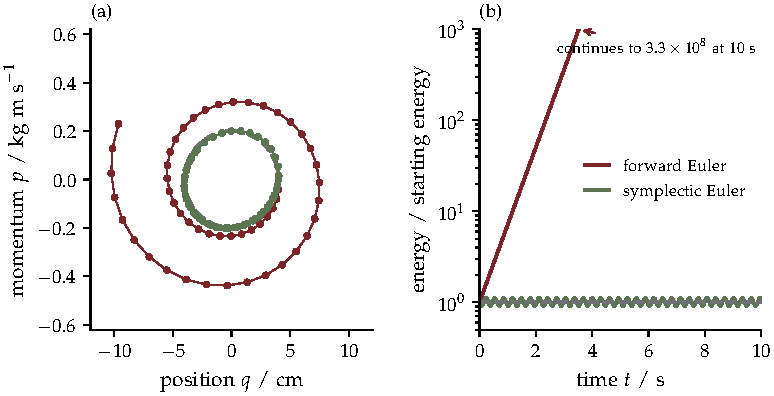
\includegraphics{ch07_hamilton/maps}
\caption{The block of \SI{0.5}{\kilogram} on a spring of
\SI{50}{\newton\per\metre} ($\omega = \SI{10}{\radian\per\second}$),
released from rest at \SI{4}{\centi\metre}, stepped with $\dt =
\SI{0.02}{\second}$ by the forward Euler method (oxblood) and the
symplectic Euler method (green). (a) The states after each step for
\SI{1}{\second}, with the true ellipse (dashed), which the green points
nearly hide. (b) The energy over \SI{10}{\second} as a
multiple of its starting value, on a logarithmic axis; the forward Euler
energy leaves the axis, at 1000 times its starting value, after
\SI{3.5}{\second}.}
\label{fig:ha-maps}
\end{figure}

With the same step of \SI{0.02}{\second}, the symplectic Euler method keeps
the block's energy between 0.9091 and 1.1111 times its starting value,
over \SI{10}{\second} and over \SI{2000}{\second} alike
(\cref{fig:ha-maps}b): its error oscillates and does not grow. Halving the
step to \SI{0.01}{\second} narrows the band to between 0.9524 and 1.0526.
Chapter~9 explains why: a step map that keeps area keeps a slightly
different energy, exactly for the spring and very nearly in
general\cite{LeimkuhlerMatthews2015}, and so stays close to the true one.
It also finds methods whose band is much narrower for the same step.

\begin{practice}
The total energy of an isolated system is the first diagnostic of a
method of computing motion and of its step. A steady growth or fall shows
a method that does not keep area, as here, a step too long for the
method, or forces that are not the slopes of a single potential energy
(\cref{sec:en-drift}); for smooth forces and sufficiently short stable steps, the symplectic
method shown here has bounded fluctuations that shrink as the step is
shortened. Chapter~9 sizes the step from these
fluctuations.
\end{practice}

\begin{keyidea}
A step map keeps area when its Jacobian determinant is 1. The forward Euler
method multiplies the spring's energy and every area by $1 + \omega^2
\dt^2$ at each step; the symplectic Euler method, a kick then a drift, keeps
area and holds the energy within a band.
\end{keyidea}

\notebook{07}{step the spring with both methods and watch a square of states}

\begin{selfcheck}
With $\omega\dt = 0.05$, by what factor does the forward Euler method
multiply the energy of a spring in 100 steps?
\end{selfcheck}

%=============================================================================!
% 7.S  WHAT WE NOW HAVE                                                       !
%=============================================================================!
\unnumbered{What we now have}

The Legendre transform of the Lagrangian in the velocities is the
Hamiltonian $H(q, p) = \sum_k p_k\dot{q}_k - \Lag$, which for a kinetic
energy quadratic in the velocities is the energy $K + U$ written in terms
of the coordinates and their momenta. Hamilton's equations, $\dot{q} =
\partial H/\partial p$ and $\dot{p} = -\partial H/\partial q$, move every
state of phase space along a flow that runs on the contours of $H$; for
the pendulum the contours show the swinging and the circulating motions
and the separatrix between them, along which the bob creeps towards the
top as $\mathrm{e}^{-\omega_0t}$. Any quantity changes at the rate $\pb{A}
{H} = \Liou A$, and the
Taylor series in the Liouville operator gives the motion from the
starting state, at every time for the ball and the spring and over a
short time in general.

The flow has no divergence, so it keeps
the area of every region of phase space, and its Jacobian determinant is
1 (Liouville's theorem); drag shrinks areas as $\mathrm{e}^{-\gamma t}$.

Every symmetry of the Lagrangian under a change that can be made as small
as we like, and the passing of time, gives a conserved quantity
(Noether's theorem): the energy from
the passing of time, the momentum from moving everything, the angular
momentum from turning everything, with no assumption about pairs of
forces; in a periodic box the momentum survives and the angular momentum
does not. For a time-independent Hamiltonian that is even in the momenta,
reversing every momentum makes the system retrace its path. Drag breaks
this reversal symmetry.

A method of computing motion is a step map:
the forward Euler method inflates the areas and the energy of a spring by
$1 + \omega^2\dt^2$ at every step, while the symplectic Euler method, a kick
followed by a drift, keeps area and holds the energy within a band.

Chapter~8 asks where the potential energy $U$ of atoms comes from, and
Chapter~9 returns to step maps and builds the methods with which
molecular dynamics is done.

%=============================================================================!
% 7.A  ANSWERS TO THE CHECKS                                                  !
%=============================================================================!
\unnumbered{Answers to the checks}
\label{sec:ha-answers}

\answerto{sec:ha-legendre}$H = p^2/(2\times2) + \frac12\times8\,x^2 =
p^2/4 + 4x^2$, in joules for $p$ in \si{\kilogram\metre\per\second} and $x$
in metres. At $x = 0$ all the energy is kinetic, $p^2/4 = 1$, so $p =
\pm\SI{2}{\kilogram\metre\per\second}$.

\answerto{sec:ha-equations}$\dot{q} = \partial H/\partial p = p/m$ and
$\dot{p} = -\partial H/\partial q = -mg$. On a contour $H = E$, $q =
E/(mg) - p^2/(2m^2g)$: parabolas with their tips at the greatest height
$E/(mg)$, where $p = 0$, opening towards smaller heights. Since $\dot{p} =
-mg$ everywhere, every state moves steadily towards smaller $p$ along its
parabola, rising while $p > 0$ and falling after.

\answerto{sec:ha-brackets}$\Liou(qp) = \dot{q}\,p + q\,\dot{p} = p^2/m -
kq^2$, by the product rule. It is zero where $p^2/m = kq^2$, that is $p =
\pm\sqrt{mk}\,q$, the two lines through the origin on which the kinetic
and potential energies are equal.

\answerto{sec:ha-liouville}$\mathcal{A} = \SI{1}{\joule\second}\times
\mathrm{e}^{-0.5\times4} = \mathrm{e}^{-2}\,\si{\joule\second} =
\SI{0.135}{\joule\second}$.

\answerto{sec:ha-noether}The $y$ and $z$ components. Moving every atom
along $y$ or $z$ carries the atoms and their copies along the wall,
changing nothing, so the $y$ and $z$ components of the forces still add to zero. Moving them along $x$
changes their distances from the fixed wall, and so their energy: the
wall's push is a force from outside the atoms, and $P_x$ is not
conserved.

\answerto{sec:ha-reversal}At the top $p = 0$, and reversing a zero momentum
changes nothing, so the motion after the top is the reversed motion before
it: the ball comes back to the hand \SI{1.224}{\second} after passing the
top, about \SI{2.45}{\second} after it was thrown, moving downwards at
\SI{12}{\metre\per\second}.

\answerto{sec:ha-symplectic}$(1 + 0.05^2)^{100} = 1.0025^{100} = 1.284$.

%=============================================================================!
% 7.E  EXERCISES                                                              !
%=============================================================================!
\unnumbered{Exercises}
\label{sec:ha-exercises}

The exercises run from questions of understanding, through calculations,
to short derivations marked `show that'. Full solutions are in
\hyperref[sec:ha-solutions]{`Solutions to the exercises'} at the end of
the book, and Notebook~07 checks every numerical answer.

\begin{exercise}[a transform with a logarithm]
\label{ex:ha-exp}
Show that the Legendre transform of $f(v) = \mathrm{e}^v$ is $f^*(p) =
p\ln p - p$, for $p > 0$, and that its slope is $v$.
\end{exercise}

\begin{exercise}[two rates in one term]
\label{ex:ha-cross}
A kinetic energy $K = \frac12(a\dot{q}_1^2 + 2b\,\dot{q}_1\dot{q}_2 +
c\,\dot{q}_2^2)$, with constants $a$, $b$ and $c$, contains a product of
two rates. Show that $p_1\dot{q}_1 + p_2\dot{q}_2 = 2K$, so that again
$H = K + U$.
\end{exercise}

\begin{exercise}[a hanging spring]
\label{ex:ha-vertical}
A block of mass $m$ hangs from a spring of stiffness $k$, with $q$ its
distance below the point where the spring has its natural length, so that
$U = \frac12 kq^2 - mgq$. Write $H$ and Hamilton's equations, and find the
state that does not change.
\end{exercise}

\begin{exercise}[a ball in a vertical plane]
\label{ex:ha-plane}
For $\Lag = \frac12 m(\dot{x}^2 + \dot{y}^2) - mgy$, find $p_x$, $p_y$
and $H$, write Hamilton's equations, and say which momentum is conserved
and why.
\end{exercise}

\begin{exercise}[the puck]
\label{ex:ha-puck}
Show that the puck of \cref{sec:la-polar}, with $\Lag = \frac12 m(\dot{r}^2
+ r^2\dot\theta^2) - U(r)$, has $H = p_r^2/(2m) + p_\theta^2/(2mr^2) +
U(r)$, and that Hamilton's equations give the conservation of $p_\theta$
and the motion of $r$ in the effective potential \cref{eq:la-effective}.
\end{exercise}

\begin{exercise}[the bead from its Hamiltonian]
\label{ex:ha-bead}
Show that Hamilton's equations for $H = p^2/\bigl(2m(1 + h'^2)\bigr) +
mgh(x)$ give the bead's equation \cref{eq:la-bead}.
\end{exercise}

\begin{exercise}[over the top]
\label{ex:ha-separatrix}
For the pendulum of \cref{fig:ha-portrait}, find the momentum and the
speed of the bob at the bottom of the separatrix.
\end{exercise}

\begin{exercise}[the last ten degrees]
\label{ex:ha-creep}
Using $\dot\varphi \approx -\omega_0\varphi$, how long does the bob of
\cref{fig:ha-portrait}, on its separatrix, take to go from \ang{10} short
of the top to \ang{1} short?
\end{exercise}

\begin{exercise}[a product rule for brackets]
\label{ex:ha-product}
Show that $\pb{A}{BC} = \pb{A}{B}\,C + B\,\pb{A}{C}$.
\end{exercise}

\begin{exercise}[angular momentum in Cartesian coordinates]
\label{ex:ha-lz}
A body moves in a plane with $H = (p_x^2 + p_y^2)/(2m) + U(r)$, where $r
= \sqrt{x^2 + y^2}$. Show that $L_z = xp_y - yp_x$ has $\pb{L_z}{H} = 0$.
\end{exercise}

\begin{exercise}[the momentum of the spring]
\label{ex:ha-spring-p}
Use the series \cref{eq:ha-series} to find $p(t)$ for the block on a
spring.
\end{exercise}

\begin{exercise}[a shear]
\label{ex:ha-shear}
A body of \SI{1}{\kilogram} flies freely. Where does the flow over
\SI{2}{\second} carry the four corners of the square of starting states
$0 \le q_0 \le \SI{0.1}{\metre}$, $0 \le p_0 \le
\SI{0.1}{\kilogram\metre\per\second}$, and what is the area of the
figure they make?
\end{exercise}

\begin{exercise}[half the area]
\label{ex:ha-halving}
With drag at $\gamma = \SI{0.5}{\per\second}$, how long does a blob of
states take to lose half its area?
\end{exercise}

\begin{exercise}[two carts]
\label{ex:ha-carts}
For the two carts of \cref{ex:la-carts}, $\Lag = \frac12 m_1\dot{x}_1^2 +
\frac12 m_2\dot{x}_2^2 - \frac12 k(x_2 - x_1 - \ell)^2$, use Noether's
theorem to show that $m_1\dot{x}_1 + m_2\dot{x}_2$ is conserved.
\end{exercise}

\begin{exercise}[under gravity]
\label{ex:ha-gravity}
A group of atoms with an energy $U_{\mathrm{int}}$ that is unchanged by
moving or turning the whole group falls in a uniform field of gravity
along $-z$, so $U = U_{\mathrm{int}} + \sum_im_igz_i$. Which components
of the total momentum, and of the angular momentum about the origin, are
conserved?
\end{exercise}

\begin{exercise}[the torque about any point]
\label{ex:ha-torque-point}
Show that when the forces on a group add to zero, their torque is the
same about every point, and find the torque of the two atoms of
\cref{fig:ha-noether}(b) about the centre of the box, $(5,
5)$~\si{\angstrom}.
\end{exercise}

\begin{exercise}[which can be reversed?]
\label{ex:ha-even}
For which of $H_1 = p^2/(2m) + U(q)$, $H_2 = (p - c)^2/(2m)$ with a
constant $c \ne 0$, and $H_3 = p^2/(2m) + \frac12 kq^2 + bqp$ with a
constant $b \ne 0$ does the argument of \cref{sec:ha-reversal} show that
reversing the momentum retraces the path?
\end{exercise}

\begin{exercise}[doubling the energy]
\label{ex:ha-doubling}
The forward Euler method follows the block of \cref{fig:ha-maps} with
$\dt = \SI{0.005}{\second}$. After how many steps, and how long, has the
energy doubled?
\end{exercise}

\begin{exercise}[the other order]
\label{ex:ha-other}
The other symplectic Euler method moves the position first, $q' = q +
\dt\,p/m$, then the momentum with the force at the new position, $p' =
p - \dt\,kq'$. Show that for the spring its Jacobian determinant is 1.
\end{exercise}

\begin{exercise}[the energy the method keeps]
\label{ex:ha-shadow}
Show that a step of the symplectic Euler method of
\cref{sec:ha-symplectic} leaves $\tilde{H} = p^2/(2m) + \frac12 kq^2 -
\bigl(k\dt/(2m)\bigr)\,qp$ unchanged for the spring.
\end{exercise}


%=============================================================================!
% CHAPTER 8  POTENTIAL ENERGY SURFACES AND INTERATOMIC MODELS                 !
%=============================================================================!
\chapter{Potential energy surfaces and interatomic models}
\label{ch:potentials}

%=============================================================================!
% 8.0  CHAPTER OPENING                                                        !
%=============================================================================!
The preceding chapters treated the potential energy $U(\vb{r}^N)$ as a
known function and used its derivatives to determine the motion. For an
atomistic simulation we must also choose how to obtain that function.
Within the Born--Oppenheimer approximation, the electrons remain in their
ground state as the nuclei move, and their energy together with the
nuclear repulsion defines the potential energy surface. Evaluating an
electronic-structure calculation at every step is costly, which motivates
simpler interatomic models.

We begin by examining when classical motion of the nuclei is an
appropriate approximation. Pair potentials then give a direct route from
an energy model to forces, their numerical checks and the treatment of a
cutoff. Their limitations motivate environment-dependent interactions for
metals and carbon, and bonded force fields for molecules. Finally, the
slow decay of the Coulomb interaction shows why charges need a separate
summation method. Chapter~9 uses these forces to advance the motion,
while Chapter~18 introduces the learning methods used to represent a
potential energy surface. Later chapters on these models are planned
for the continuation of Part~V.

%=============================================================================!
% 8.1  WHERE THE POTENTIAL ENERGY COMES FROM                                  !
%=============================================================================!
\section{Where the potential energy comes from}
\label{sec:pe-origin}

An atom is a small, heavy nucleus surrounded by much lighter electrons.
The forces between atoms are the electrical attractions and repulsions of
these charges: nuclei repel nuclei, electrons repel electrons, and each
attracts the other. This section explains how the motion of the electrons
can be set aside, leaving a potential energy for the nuclei alone, and
what it costs to compute it.

\subsection*{Heavy nuclei, light electrons}

A proton is 1836 times as heavy as an electron, and a lithium atom, of
mass \SI{6.94}{amu} (\cref{sec:ne-atoms}), 12\,651 times, almost all of
it in the nucleus. Pushed by forces of similar size, a body's acceleration is
inversely proportional to its mass, and \cref{sec:os-small} showed that a
body held by a spring of stiffness $k$ swings with $\omega_0 =
\sqrt{k/m}$: with comparable stiffnesses, the electrons respond
$\sqrt{1836} = 43$ times faster than a proton and 112 times faster than
lithium. On the time scale on which the nuclei move, the electrons
have time to settle into the arrangement of lowest energy for wherever
the nuclei happen to be, and to follow them as they move.

This is the picture of Born and Oppenheimer\cite{BornOppenheimer1927}.
With the nuclei held still at the positions $\vb{r}^N$, the electrons
settle into their state of lowest energy for those positions, and that
energy, together with the repulsion of the nuclei for one another,
depends only on $\vb{r}^N$; we call it $U(\vb{r}^N)$. When the nuclei move, the electrons
follow, and the nuclei move as if pushed by the forces $-\grad_iU$
(\cref{sec:en-atoms}). The function $U$ is called the potential energy
surface: for a single coordinate it is a curve, for two a landscape like
that of the lithium atom on its model layer (\cref{sec:en-surface}), and
for $N$ atoms a surface in $3N$ dimensions. The picture fails when the
motion of the nuclei carries the electrons from one state into another
close in energy, as after light is absorbed or in some chemical
reactions; every system in this book stays in its lowest state.

\subsection*{The cost of computing it}

Finding the lowest state of the electrons is a problem of quantum
mechanics. Density-functional theory, one such method, turns it into the eigenvalues and eigenvectors (\cref{sec:os-modes}) of a
matrix whose size $n$ grows in proportion to the number of atoms. The
work of finding all of them grows as $n^3$, and \cref{fig:pe-cost}(a)
measures it:
with NumPy, doubling the size of a dense symmetric matrix multiplied the
time to find its eigenvalues and eigenvectors by about 7.5, close to $2^3 =
8$, and the times for the larger matrices lie near a line of slope 3 on
logarithmic axes
(\cref{sec:mo-taylor}): a time proportional to $n^3$ has a logarithm that
grows by 3 times the logarithm of $n$. The energy of a model that adds up the energies of
pairs of atoms needs one term for each pair: each of the $N$ atoms pairs
with $N - 1$ others, which counts every pair twice, so there are $N(N -
1)/2 \approx N^2/2$ pairs for large $N$, a number that doubling $N$
multiplies by $2^2 = 4$; doubling $N$ multiplied its time by about 4
(\cref{fig:pe-cost}b); with the cutoffs of \cref{sec:pe-cutoffs} and the
neighbour lists of Chapter~10 it grows only as $N$. Computing $U$ from the
electrons at every step of a simulation therefore limits it to far
smaller systems and shorter times than a model allows, and most
simulations use a model of $U$ fitted to such calculations, which is the subject of the rest of this
chapter.

\begin{figure}[htb]
\centering
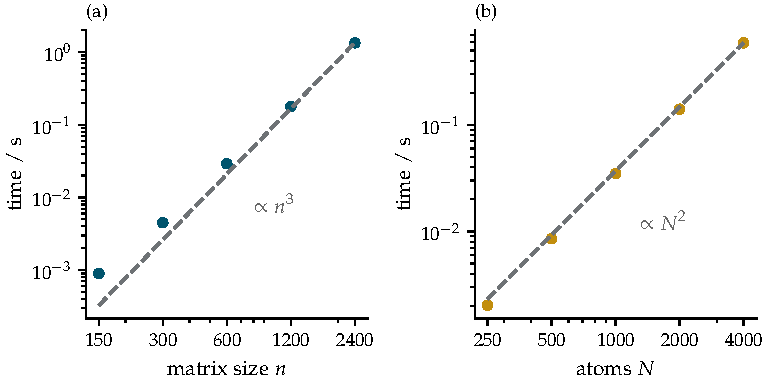
\includegraphics{ch08_potentials/cost}
\caption{What computing the energy costs, with NumPy on one processor
core; the times depend on the computer, the slope at large sizes does
not. (a) Finding
all the eigenvalues and eigenvectors of a dense symmetric matrix of size
$n$ (one with no zero entries to exploit), against $n$, with a line of
slope 3 (dashed). (b) The energy and forces of $N$ atoms interacting in
pairs, every pair computed, against $N$, with a line of slope 2
(dashed).}
\label{fig:pe-cost}
\end{figure}

\begin{bridge}
The forces on the nuclei follow from the electronic energy by the
Hellmann--Feynman theorem\cite{Feynman1939}: at the converged density they
are the electrostatic forces of the electrons and the other nuclei, plus
Pulay corrections when the basis functions move with the atoms. The
cubic cost is that of a dense eigensolver; linear-scaling methods use the
nearsightedness of the density matrix to reach a cost proportional to
$N$\cite{Kohn1996}, and machine-learned potentials (planned for the
continuation of Part~V) build the same
locality into a model fitted to the expensive calculations.
\end{bridge}

\begin{keyidea}
Because the electrons are light and fast, they settle at every
arrangement of the nuclei, and the energy of that settled state, with the
repulsion of the nuclei, is the potential energy surface $U(\vb{r}^N)$ on
which the nuclei move. Computing it from the electrons costs, in the usual
methods, work growing as the cube of the system's size, which is why most simulations fit a
model of it.
\end{keyidea}

\begin{selfcheck}
Finding all the eigenvalues and eigenvectors of a matrix of size 1000
takes \SI{0.1}{\second}. Roughly how long does it take for one of size
4000?
\end{selfcheck}

%=============================================================================!
% 8.2  WHEN THE NUCLEI ARE CLASSICAL                                          !
%=============================================================================!
\section{When the nuclei may be treated as classical}
\label{sec:pe-classical}

The electrons need quantum mechanics; this book moves the nuclei by
Newton's laws, which \cref{sec:ne-atoms} called an approximation. This
section finds when it is a good one, from a comparison of two energies.

Quantum mechanics changes the motion of a vibration in one way that
matters here: a harmonic oscillator (\cref{sec:os-small}) of angular frequency $\omega$
cannot have any energy it likes, only the values $(n + \frac12)\hbar\omega$, with $n = 0,
1, 2, \dots$ and $\hbar = \SI{0.6582}{\electronvolt\femto\second}$ the
reduced Planck constant\cite{Tuckerman2023}. Its energy therefore comes
in steps of $\hbar\omega$, and even in its lowest state, $n = 0$, it keeps the energy
$\frac12\hbar\omega$, its zero-point energy, which a classical oscillator
lacks. At a temperature $T$, the motion of each vibration carries a
typical energy of order $\kB T$, where $\kB$ is Boltzmann's constant and
$\kB T = \SI{0.02585}{\electronvolt}$ at \SI{300}{\kelvin}
(Chapter~12 makes this precise). When $\hbar\omega \ll \kB T$, a typical
vibration spans many steps, too small to notice, and the classical
description is good. When $\hbar\omega \gg \kB T$, the vibration
sits in its lowest state, and a classical model, which lets it lose its
zero-point energy, describes it wrongly.

With $\omega = 2\pi\nu = 2\pi c\tilde\nu$ for a wavenumber $\tilde\nu$
(\cref{sec:os-molecules}), $\hbar\omega = 2\pi\hbar c\,\tilde\nu$, and
$2\pi\hbar c = \SI{1.2398e-4}{\electronvolt\centi\metre}$. At \SI{300}{\kelvin}:
\begin{itemize}
\item the symmetric O--H stretch of water, \SI{3657}{\per\centi\metre}
   (\cref{tab:os-vibrations}), has $\hbar\omega = \SI{0.4534}{\electronvolt}$,
   17.5 times $\kB T$: thoroughly quantum;
\item the stretch of LiF, \SI{910.34}{\per\centi\metre}
   (\cref{sec:ro-molecules}), has $\hbar\omega =
   \SI{0.1129}{\electronvolt}$, 4.4 times $\kB T$;
\item the model lithium atom rattling in its hollow with a period
   $\mathcal{T} = \SI{170.3}{\femto\second}$ (\cref{sec:os-small}) has $\hbar\omega =
   \hbar\,2\pi/\mathcal{T} = \SI{0.0243}{\electronvolt}$, 0.94 times $\kB
   T$: borderline at room temperature, and 2.8 times $\kB T$ at
   \SI{100}{\kelvin}.
\end{itemize}
The lighter the atom and the stiffer its bonds, the larger $\omega$ and
the stronger the quantum character, so the motion of hydrogen is where
classical nuclei fail first: quantum effects of the nuclei can change
measured properties of water and other hydrogen-bonded systems at room
temperature\cite{MarklandCeriotti2018}. A bond between heavier atoms can
still be quantum, as LiF shows, and the rattle of lithium in its hollow
is borderline. The motions this book measures, the turning and drifting
of whole molecules and the hops of lithium and other ions heavier than
hydrogen, we follow with classical nuclei, accepting that the energy of
the fast stretches is then wrong.
Methods that keep the quantum character of the nuclei exist; they are
beyond the scope of this book.

\begin{keyidea}
A vibration may be treated classically when its quantum step
$\hbar\omega = 2\pi\hbar c\,\tilde\nu$ is small compared with $\kB T$. At room
temperature this holds for slow motions, is borderline for the rattle of
lithium in its hollow, and fails for the stretches of chemical bonds,
most of all bonds to hydrogen.
\end{keyidea}

\begin{selfcheck}
Is the C--H stretch, near \SI{3000}{\per\centi\metre}, classical at
\SI{300}{\kelvin}?
\end{selfcheck}

%=============================================================================!
% 8.3  PAIR POTENTIALS                                                        !
%=============================================================================!
\section{Pair potentials}
\label{sec:pe-pairs}

The simplest model of $U$ adds up an energy for each pair of atoms that
depends only on the distance between them,
\begin{equation}
   U(\vb{r}^N) = \sum_{i<j}\varphi(r_{ij}) ,
   \label{eq:pe-pair-sum}
\end{equation}
where the sum runs over every pair once: $i$ takes each value from 1 to
$N$ and, for each $i$, $j$ each value from $i + 1$ to $N$, so
$\varphi(r_{12})$ enters but not $\varphi(r_{21})$; $\varphi$ is called a
pair potential. It ignores any effect that a third atom has on the
energy of a pair, which makes it a reasonable first model for atoms that
keep their electrons to themselves, such as those of the noble gases, and a poor one
for metals and for atoms joined by chemical bonds (\cref{sec:pe-manybody,%
sec:pe-bonded}). \Cref{sec:os-anharmonic} met the two most common shapes;
this section adds a third and compares them.

\subsection*{Three shapes}

The Lennard-Jones potential,
\begin{equation*}
   \varphi_{\mathrm{LJ}}(r) = 4\varepsilon\Bigl[\Bigl(\frac{\sigma}{r}
   \Bigr)^{12} - \Bigl(\frac{\sigma}{r}\Bigr)^6\Bigr] ,
\end{equation*}
has its minimum, of depth $\varepsilon$, at $r_{\mathrm m} =
2^{1/6}\sigma = 1.1225\,\sigma$ (written $r_{\min}$ in
\cref{sec:os-anharmonic}). Its attraction
falls as $r^{-6}$, the form of the weak attraction between neutral atoms
far apart, and its repulsion, $r^{-12}$, is steep and cheap to compute as
the square of $r^{-6}$; inverse powers of this kind go back to
Jones\cite{Jones1924}. For argon, $\varepsilon/\kB = \SI{120}{\kelvin}$,
so $\varepsilon = \SI{0.01034}{\electronvolt}$, and $\sigma =
\SI{3.4}{\angstrom}$: the values with which Rahman made the first
simulation of a real liquid by molecular dynamics\cite{Rahman1964}.

The Morse potential of \cref{sec:os-anharmonic} describes a chemical bond
between two atoms\cite{Morse1929}. Written there with its least value 0,
it is lowered here by $D$, so that, like every pair potential in a sum
\cref{eq:pe-pair-sum}, it is zero for atoms far apart:
\begin{equation*}
   \varphi_{\mathrm M}(r) = D\bigl(1 - \mathrm{e}^{-a(r - r_0)}\bigr)^2 - D
   = D\bigl(\mathrm{e}^{-2a(r - r_0)} - 2\,\mathrm{e}^{-a(r - r_0)}\bigr) ,
\end{equation*}
expanding the square, $1 - 2\mathrm{e}^{-a(r-r_0)} +
\mathrm{e}^{-2a(r-r_0)}$, multiplying by $D$ and cancelling the resulting
$D$ against $-D$. Its minimum
is $-D$ at $r_0$, and its stiffness there is $2Da^2$, as before.

The Buckingham potential replaces the $r^{-12}$ wall by an exponential,
\begin{equation*}
   \varphi_{\mathrm B}(r) = A\,\mathrm{e}^{-r/\rho} - \frac{C}{r^6} ,
\end{equation*}
with a strength $A$ and a range $\rho$ for the repulsion (a local
constant, unrelated to the $\rho_i$ of \cref{sec:pe-manybody}) and a
strength $C$ for the attraction\cite{Buckingham1938}. Written with
the position $r_{\mathrm m}$ and depth $\varepsilon$ of its minimum and a
steepness $\alpha$, as $A = 6\varepsilon\,\mathrm{e}^{\alpha}/(\alpha -
6)$, $\rho = r_{\mathrm m}/\alpha$ and $C = \alpha\varepsilon r_{\mathrm
m}^6/(\alpha - 6)$ (\cref{ex:pe-exp6}), it is called the exp-6 potential.

\Cref{fig:pe-pairs} compares the three with the same minimum,
$-\varepsilon$ at $r_{\mathrm m}$. The Lennard-Jones stiffness there is
$57.15\,\varepsilon/\sigma^2$ (\cref{sec:os-anharmonic}), which with
$\sigma^2 = r_{\mathrm m}^2/2^{1/3}$ is $57.15\times2^{1/3}\,\varepsilon/
r_{\mathrm m}^2 = 72\,\varepsilon/r_{\mathrm m}^2$; the Morse width
$a r_{\mathrm m} = 6$ matches it, since $2Da^2 = 2\varepsilon\times36/
r_{\mathrm m}^2$, and the exp-6 steepness $\alpha = 14$ gives $73.5\,
\varepsilon/r_{\mathrm m}^2$, within 2\% of it. Near the minimum they
agree; at $r = 2r_{\mathrm m}$ the Lennard-Jones and exp-6 energies are
$-0.031\varepsilon$ and $-0.027\varepsilon$, falling as $r^{-6}$, while
the Morse energy, $-0.005\varepsilon$, falls exponentially; and close in
they differ completely: the Lennard-Jones wall rises without limit; the Morse energy
stays finite, $\num{1.6e5}\,\varepsilon$ at $r = 0$; and the exp-6 energy
rises to a maximum of $\num{2.8e4}\,\varepsilon$ at $0.203\,r_{\mathrm m}$
and then falls to $-\infty$, because as $r \to 0$ the term $-C/r^6$ grows
without limit while $A\,\mathrm{e}^{-r/\rho}$ approaches $A$. With
$\alpha = 14$ that maximum is far out of thermal reach, but it falls
steeply as $\alpha$ is lowered, and for some fitted parameter sets a very
hot simulation can push two atoms past it, after which they fall into
each other.

\begin{figure}[htb]
\centering
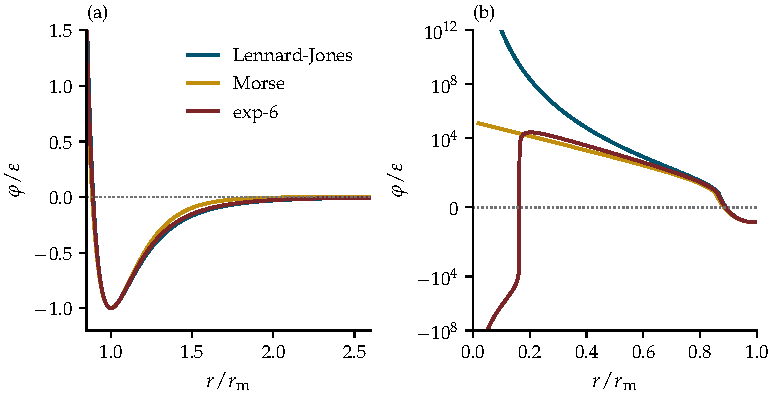
\includegraphics{ch08_potentials/pairs}
\caption{The Lennard-Jones, Morse ($a r_{\mathrm m} = 6$) and exp-6
($\alpha = 14$) pair potentials with the same minimum $-\varepsilon$ at
$r_{\mathrm m}$. (a) Near the well. (b) The wall, on a scale that is
logarithmic beyond $\pm1$: the Lennard-Jones energy rises without limit,
the Morse energy rises only exponentially, a straight line here, to a
finite value at $r = 0$, and the exp-6 energy turns over and falls.}
\label{fig:pe-pairs}
\end{figure}

\subsection*{Reduced units}

For atoms that interact only by a Lennard-Jones potential, the constants
$\varepsilon$, $\sigma$ and the mass $m$ can be removed from the equations
of motion altogether. We measure lengths in units of $\sigma$, energies in
units of $\varepsilon$ and times in units of a time $\tau$ still to be
chosen, so we write $\vb{r}_i = \sigma\vb{r}_i^*$, $U = \varepsilon U^*$ and
$t = \tau t^*$, where the starred quantities are pure numbers. By the
chain rule, with $t^* = t/\tau$, $\dd\vb{r}_i/\dd t = \sigma\,(\dd
\vb{r}_i^*/\dd t^*)(\dd t^*/\dd t) = (\sigma/\tau)\,\dd\vb{r}_i^*/\dd t^*$,
and once more $\ddot{\vb{r}}_i = (\sigma/\tau^2)\,\dd^2\vb{r}_i^*/\dd
t^{*2}$; likewise $\partial U/\partial x_i = \varepsilon\,(\partial U^*/
\partial x_i^*)(\dd x_i^*/\dd x_i) = (\varepsilon/\sigma)\,\partial U^*/
\partial x_i^*$, so $\grad_iU = (\varepsilon/\sigma)\grad_i^*U^*$, and the
second law $m\ddot{\vb{r}}_i = -\grad_iU$ becomes
\begin{align*}
   \frac{m\sigma}{\tau^2}\,\frac{\dd^2\vb{r}_i^*}{\dd t^{*2}}
   &= -\frac{\varepsilon}{\sigma}\,\grad_i^*U^*\\
   \frac{\dd^2\vb{r}_i^*}{\dd t^{*2}}
   &= -\frac{\varepsilon\tau^2}{m\sigma^2}\,\grad_i^*U^*
   && \text{multiplying by $\tau^2/(m\sigma)$,}
\end{align*}
and, since $\sigma/r_{ij} = 1/r_{ij}^*$, $U^* = \sum
4[(r_{ij}^*)^{-12} - (r_{ij}^*)^{-6}]$ contains no constants. Choosing
\begin{equation}
   \tau = \sigma\sqrt{\frac{m}{\varepsilon}}
   \label{eq:pe-tau}
\end{equation}
makes the factor 1, and the equation is the same for every substance of
this kind: one simulation in reduced units describes argon, krypton or
any other, each with its own $\varepsilon$, $\sigma$ and $m$, converting
back by $\sigma$, $\varepsilon$ and $\tau$, as far as the real atoms
interact by a Lennard-Jones potential and move classically. For argon,
of mass \SI{39.948}{amu}, $\varepsilon = 0.01034\times\num{9.648533e-3}
= \num{9.977e-5}$ in amu\,\AA$^2$/fs$^2$ (\cref{sec:ne-atoms}), so $\tau
= 3.4\times\sqrt{39.948/\num{9.977e-5}} = \SI{2151}{\femto\second}$,
about \SI{2.15}{\pico\second}.

\begin{keyidea}
A pair potential adds up an energy $\varphi(r_{ij})$ for every pair. The
Lennard-Jones, Morse and exp-6 shapes agree near their minimum and differ
in the tail and the wall; the exp-6 wall turns over. In units of
$\sigma$, $\varepsilon$ and $\tau = \sigma\sqrt{m/\varepsilon}$, all
Lennard-Jones substances obey the same equations.
\end{keyidea}

\notebook{08}{compare the three pair potentials and their forces}

\begin{selfcheck}
Krypton has $\varepsilon/\kB \approx \SI{160}{\kelvin}$, $\sigma \approx
\SI{3.6}{\angstrom}$ and a mass of \SI{83.8}{amu}. Is its $\tau$ longer or
shorter than argon's, and why?
\end{selfcheck}

%=============================================================================!
% 8.4  FORCES, THE VIRIAL, AND CHECKING FORCES                                !
%=============================================================================!
\section{Forces, the virial, and checking forces}
\label{sec:pe-forces}

A simulation needs the force on every atom at every step, and a few other
sums computed alongside it. This section derives them for a pair
potential, shows the code that computes them, and shows how to check any
force routine against its energy.

\subsection*{Forces}

Atom $i$ appears in the sum \cref{eq:pe-pair-sum} in the $N - 1$ terms
$\varphi(r_{ij})$ with $j \ne i$. \Cref{sec:ro-system} found the gradient
of one such term, $-\grad_i\varphi(r_{ij}) = \varphi'(r_{ij})\,\vb{r}_{ij}/
r_{ij}$ with $\vb{r}_{ij} = \vb{r}_j - \vb{r}_i$, so
\begin{equation}
   \vb{F}_i = \sum_{j\ne i}\varphi'(r_{ij})\,\frac{\vb{r}_{ij}}{r_{ij}} .
   \label{eq:pe-pair-force}
\end{equation}
Each term is the force on $i$ from $j$, along the line joining them,
towards $j$ when $\varphi' > 0$, where the energy rises with distance and
the pair attracts. The force on $j$ from $i$ is the same with $i$ and $j$
exchanged, and since $\vb{r}_{ji} = -\vb{r}_{ij}$ it is equal and
opposite: Newton's third law (\cref{sec:ne-third}). A program therefore
computes each pair once and adds its force to one atom and subtracts it
from the other, which is what \texttt{pair\_energy\_forces} of
\texttt{mdlab} does:

\begin{code}
def pair_energy_forces(
    positions: ArrayLike, pair: PairFunction
) -> tuple[float, NDArray, float]:
    r = np.asarray(positions, dtype=float)
    n = len(r)
    i, j = np.triu_indices(n, k=1)  # every pair once
    rij = r[i] - r[j]
    dist = np.linalg.norm(rij, axis=1)
    phi, dphi = pair(dist)
    f_on_i = -(dphi / dist)[:, None] * rij  # force on i from j
    forces = np.zeros_like(r)
    np.add.at(forces, i, f_on_i)
    np.add.at(forces, j, -f_on_i)
    return float(phi.sum()), forces, float(-(dist * dphi).sum())
\end{code}

\noindent \texttt{np.triu\_indices(n, k=1)} lists the pairs $(i, j)$ with
$i < j$ as two arrays of the same length; \texttt{rij} holds $\vb{r}_i -
\vb{r}_j = -\vb{r}_{ij}$ for every pair at once, so the minus sign makes
\texttt{f\_on\_i} the force of \cref{eq:pe-pair-force}; and
\texttt{np.add.at} adds each pair's force into the row of its atom, even
when an atom appears in many pairs; the plainer \texttt{forces[i] +=
f\_on\_i} would keep only one force for an atom listed several times in
\texttt{i}. The argument \texttt{pair} is any
function that returns $\varphi$ and $\varphi'$ for an array of distances,
such as \texttt{lennard\_jones}.

\subsection*{The virial}

The last number returned is the virial, $\mathcal{W} = \sum_i\vb{r}_i\cdot
\vb{F}_i$, from which Chapter~14 computes the pressure. For a pair potential it
takes a simple form. The pair $(i, j)$ contributes $\vb{F}_{ij}$ to atom
$i$ and $-\vb{F}_{ij}$ to atom $j$, and so $\vb{r}_i\cdot\vb{F}_{ij} -
\vb{r}_j\cdot\vb{F}_{ij} = -\vb{r}_{ij}\cdot\vb{F}_{ij}$ to $\mathcal{W}$. With
$\vb{F}_{ij} = \varphi'(r_{ij})\,\vb{r}_{ij}/r_{ij}$ and $\vb{r}_{ij}\cdot
\vb{r}_{ij} = r_{ij}^2$,
\begin{equation}
   \mathcal{W} = -\sum_{i<j} r_{ij}\,\varphi'(r_{ij}) .
   \label{eq:pe-virial}
\end{equation}
It depends only on distances, so it does not change when the origin is
moved. That holds for any potential whose forces add to zero: moving the
origin by $\vb{a}$ replaces each $\vb{r}_i$ by $\vb{r}_i - \vb{a}$ and
changes $\mathcal{W}$ by $-\vb{a}\cdot\sum_i\vb{F}_i = 0$ (\cref{sec:ha-noether}).
A pair pushed closer than its minimum repels, $\varphi' < 0$, and
contributes positively; a stretched pair attracts and contributes
negatively.

\subsection*{Checking forces}

A force routine is easy to get wrong and hard to check by eye, and a force
that is not exactly $-\grad U$ makes the energy drift (\cref{sec:en-drift}).
The standard check compares it with central differences of the energy,
$F \approx -[U(x + h) - U(x - h)]/(2h)$ for each coordinate in turn
(\cref{sec:mo-atoms}). Two errors limit the check. The Taylor series of
\cref{sec:mo-taylor} gives $U(x \pm h) = U \pm hU' + \frac12 h^2U'' \pm
\frac16 h^3U''' + \frac1{24}h^4U'''' + \order{h^5}$; subtracting cancels
the even powers, which have the same sign in both, as in
\cref{sec:mo-atoms}, so
\begin{equation*}
   \frac{U(x + h) - U(x - h)}{2h} = U' + \frac{h^2}{6}\,U''' + \order{h^4} ,
\end{equation*}
an error that shrinks as $h^2$. But a computer stores a number with about
16 significant decimal digits: rounding to the nearest stored number
changes it by at most half the machine epsilon, $\epsilon_{\mathrm m} =
2.2\times10^{-16}$ (the gap between 1 and the next stored number), times
its size, so a computed energy, a sum of many rounded terms, is uncertain
by about $\epsilon_{\mathrm m}\lvert U\rvert$ or more. The difference of two such energies
divided by $2h$ carries an error of order $\epsilon_{\mathrm m}\lvert U
\rvert/h$, which grows as $h$ shrinks. The total,
\begin{equation}
   \text{error} \approx \frac{h^2}{6}\,\lvert U'''\rvert
   + \frac{\epsilon_{\mathrm m}\lvert U\rvert}{h} ,
   \label{eq:pe-fd-error}
\end{equation}
is least where its slope with respect to $h$, $h\lvert U'''\rvert/3 -
\epsilon_{\mathrm m}\lvert U\rvert/h^2$, is zero, that is at $h^3 =
3\epsilon_{\mathrm m}\lvert U\rvert/\lvert U'''\rvert$: a step of about
the cube root of $\epsilon_{\mathrm m}$, $\num{6e-6}$, times the length on
which $U$ changes (if $U$ changes by about its own size over a length
$L$, then $\lvert U'''\rvert \approx \lvert U\rvert/L^3$ and $h \approx
(3\epsilon_{\mathrm m})^{1/3}L$); near the steep repulsion $L$ is much
shorter than $\sigma$ (\cref{ex:pe-best-step}). \Cref{fig:pe-fd} measures it for twelve Lennard-Jones
atoms. The error falls as $h^2$ (fitted slope 2.03) for large steps,
grows as $1/h$ (slope $-1.01$) for small ones, and is least,
$\num{1.0e-8}\,\varepsilon/\sigma$, at $h = 10^{-6}\sigma$, against forces
of up to $129\,\varepsilon/\sigma$.

\begin{figure}[htb]
\centering
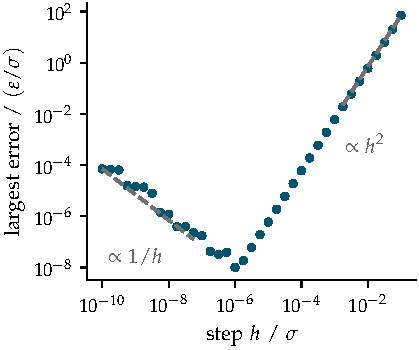
\includegraphics{ch08_potentials/fd}
\caption{The largest error of forces from central differences of the
energy, for twelve Lennard-Jones atoms, against the step $h$: falling as
$h^2$ (dashed) from the Taylor series and rising as $1/h$ (dashed) from
the rounding of the energies.}
\label{fig:pe-fd}
\end{figure}

\begin{practice}
Every new force routine, and every change to one, should be checked
against central differences of its own energy, on an arrangement of atoms
that is not symmetric, so that no error cancels. A step near
$10^{-6}$ times the distance between atoms, the best step of
\cref{fig:pe-fd}, is a good start; the check should be repeated at a step
ten times larger and smaller, and the difference should behave as
\cref{eq:pe-fd-error} predicts. The tests of \texttt{mdlab} compare every
force routine of this chapter with central differences, at one step.
\end{practice}

\begin{keyidea}
For a pair potential, $\vb{F}_i = \sum_j\varphi'(r_{ij})\,\vb{r}_{ij}/
r_{ij}$, computed once per pair and applied with opposite signs, and the
virial is $\mathcal{W} = -\sum r_{ij}\varphi'(r_{ij})$. Forces are checked against
central differences of the energy, whose error is least at a step near
$\epsilon_{\mathrm m}^{1/3}$ times the length scale.
\end{keyidea}

\notebook{08}{break a force routine on purpose and catch it}

\begin{selfcheck}
Two Lennard-Jones atoms sit at $r = \sigma$. Is their virial positive or
negative?
\end{selfcheck}

%=============================================================================!
% 8.5  CUTOFFS                                                                !
%=============================================================================!
\section{Cutoffs}
\label{sec:pe-cutoffs}

A pair potential such as the Lennard-Jones energy never reaches zero as
$r$ grows, but beyond a few $\sigma$ it is very small: at $r_{\mathrm c} = 2.5\sigma$
it is $-0.0163\varepsilon$, less than 2\% of the depth of the well.
Ignoring every pair farther apart than such a cutoff distance
$r_{\mathrm c}$ leaves each atom with a fixed number of partners, on
average, at a given density, however large the system, and with the neighbour lists of
Chapter~10 makes the cost grow as $N$ in place of $N^2$. This section
compares three ways of cutting it off.

\subsection*{Three ways to cut}

The simplest choice, truncation, keeps $\varphi$ unchanged inside
$r_{\mathrm c}$ and sets it to zero outside. The energy then jumps by
$\varphi(r_{\mathrm c})$ whenever a pair crosses the cutoff, while the
force computed from \cref{eq:pe-pair-force}, which uses only $\varphi'$,
knows nothing of the jump: the force is not the slope of the energy
reported with it at $r_{\mathrm c}$, and the total energy changes by
$\mp\varphi(r_{\mathrm c})$ at every crossing, as \cref{sec:en-drift}
warned.

Truncating and shifting subtracts the constant $\varphi(r_{\mathrm c})$
inside the cutoff,
\begin{equation*}
   \varphi_{\mathrm s}(r) = \begin{cases}
      \varphi(r) - \varphi(r_{\mathrm c}) , & r < r_{\mathrm c} ,\\
      0 , & r \ge r_{\mathrm c} ,
   \end{cases}
\end{equation*}
so that the energy is continuous. A constant has no slope, so the forces
are unchanged, and the force still jumps at $r_{\mathrm c}$, from a
pull of $\varphi'(r_{\mathrm c}) = 0.039\,\varepsilon/\sigma$ for the
Lennard-Jones potential to nothing.

Switching multiplies $\varphi$ by a function $S$ that falls smoothly from
1 to 0 between a switching distance $r_{\mathrm s}$ and $r_{\mathrm c}$.
With $x = (r - r_{\mathrm s})/(r_{\mathrm c} - r_{\mathrm s})$ running
from 0 to 1 across that range,
\begin{equation}
   S(x) = 1 - 10x^3 + 15x^4 - 6x^5
   \label{eq:pe-switch}
\end{equation}
is 1 at $x = 0$ and 0 at $x = 1$ with its first and second derivatives
zero at both ends (\cref{ex:pe-switch}); these six conditions fix the six
coefficients of a polynomial of degree five, and none of lower degree
meets them all, so the energy and the force both pass smoothly to
zero. The price is a changed force between $r_{\mathrm s}$ and
$r_{\mathrm c}$. Since $S$ depends on $r$ through $x$, the chain rule gives
$\dd S/\dd r = (\dd S/\dd x)/(r_{\mathrm c} - r_{\mathrm s})$, and the
product rule then gives the force
\begin{equation*}
   -\frac{\dd(\varphi S)}{\dd r} = -\varphi'S - \frac{\varphi}{r_{\mathrm
   c} - r_{\mathrm s}}\,\frac{\dd S}{\dd x} .
\end{equation*}
There $\varphi < 0$ and $\dd S/\dd x = -30x^2(1 - x)^2 < 0$, so the second
term is negative: a pull that the original potential does not have
(\cref{fig:pe-cutoff}b).

\begin{figure}[htb]
\centering
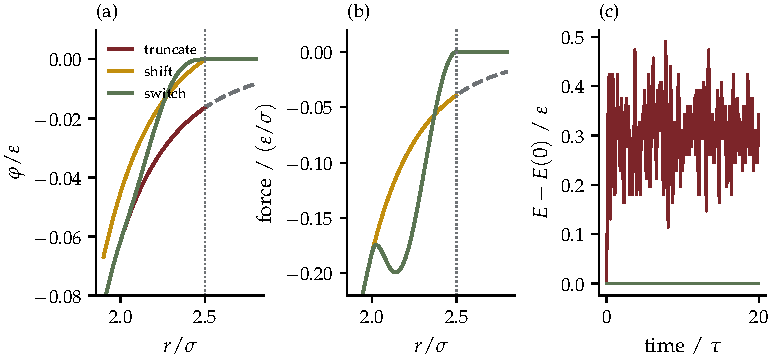
\includegraphics{ch08_potentials/cutoff}
\caption{The Lennard-Jones potential cut at $r_{\mathrm c} = 2.5\sigma$ by
truncation, truncation and shifting, and switching between $2\sigma$ and
$2.5\sigma$, with the full potential dashed. (a) The energy; the
truncated energy jumps at $r_{\mathrm c}$. (b) The force, the same for
truncation and shifting, which jump at $r_{\mathrm c}$. (c) The total
energy of 32 atoms followed for $20\tau$ by \texttt{solve\_newton} of
\texttt{mdlab}, an adaptive solver, as its change from the start: truncated
(oxblood), and without a cutoff, shifted and switched, all on the line
at zero.}
\label{fig:pe-cutoff}
\end{figure}

\subsection*{What each does to the motion}

\Cref{fig:pe-cutoff}(c) follows a cluster of 32 Lennard-Jones atoms for
$20\tau$ with \texttt{solve\_newton} of \texttt{mdlab}, which steps
Newton's equations forward with a high-order method and chooses each step
to hold its error below a set tolerance, once with each potential, and
records the total energy every $0.025\tau$. Without a cutoff it changes
by at most $\num{1.3e-10}\,\varepsilon$, the error of the solver. With
truncation it wanders by up to $0.49\varepsilon$, in jumps of up to
$0.11\varepsilon$ between successive records, each the net effect of
several crossings (seven for the largest) of $0.0163\varepsilon$ each. The motion is that of the shifted potential,
since the forces are the same, but the energy reported with it is not
conserved. Shifted and switched, the energy is
conserved to $\num{6e-8}\,\varepsilon$, some 500 times less well than
without a cutoff: $S$ of \cref{eq:pe-switch} has a third derivative that
jumps at both ends, so a higher derivative of the force still jumps
whenever a pair crosses $r_{\mathrm s}$ or $r_{\mathrm c}$.

The shifted potential pays for its jumping force in another way. The
solver chooses its own steps to keep its error below a set tolerance,
and to do so it called for the forces 26\,465 times without a cutoff and
28\,925 times with switching, but 1\,221\,089 times with truncation or
shifting, 46 times as often. Its error, like that of any method that advances
the motion step by step, rests on the Taylor series of the motion over a
step (\cref{sec:mo-taylor}), which assumes that the force changes
smoothly; a jump in the force breaks that assumption, and the solver can
only keep its accuracy by taking tiny steps across every jump. The
fixed-step methods of Chapter~9 cannot do that, and Chapter~9 measures
what a jump in the force costs them.

Machine-learned potentials face the same choice and make the smooth one.
Behler and Parrinello multiplied each neighbour's contribution by $\frac12
[\cos(\pi r/r_{\mathrm c}) + 1]$, which falls to zero with zero slope at
the cutoff distance\cite{BehlerParrinello2007}, and TrajCast (the planned Chapter~28)
multiplies by the polynomial envelope of DimeNet\cite{Gasteiger2020}, $1 - \frac12(p + 1)(p + 2)\,x^p +
p(p + 2)\,x^{p + 1} - \frac12 p(p + 1)\,x^{p + 2}$, with $x = r/r_{\mathrm
c}$ and $p = 6$, which is zero at the cutoff with its first and second
derivatives (\cref{ex:pe-envelope}).

\begin{keyidea}
A cutoff should take both the energy and the force smoothly to zero.
Truncation makes the energy jump, so the total energy is not conserved.
Shifting makes the energy continuous but leaves the force jumping, which
an adaptive solver can follow only with far shorter steps, 46 times as
many force calls here. Switching, or a smooth envelope as in
machine-learned potentials, removes both jumps, though a jump left in a
higher derivative still costs an accurate solver some accuracy.
\end{keyidea}

\notebook{08}{cut a potential three ways and watch the energy}

\begin{selfcheck}
For argon ($\varepsilon = \SI{0.01034}{\electronvolt}$), how large is each
jump of the total energy when a pair crosses a truncated cutoff at
$2.5\sigma$?
\end{selfcheck}

%=============================================================================!
% 8.6  MANY-BODY POTENTIALS                                                   !
%=============================================================================!
\section{Many-body potentials for metals and carbon}
\label{sec:pe-manybody}

In a pair potential every bond has the same strength whatever else its
atoms are bonded to. That fails for two materials used for the negative
electrodes of lithium batteries, lithium metal and graphite. In
both, the strength of a bond depends on how many other bonds its atoms
have. This section builds a model with that property, the simplest
many-body potential, and describes the forms used for metals and carbon.

\subsection*{Bonds that weaken as they multiply}

In a metal the outer electrons are shared by all the atoms, and an atom
with more neighbours spreads its share of them over more bonds, each
weaker. A model that captures this writes the energy of atom $i$ with a
square root,
\begin{equation}
   U = \sum_i\Bigl[\sum_{j\ne i}A\,\mathrm{e}^{-\eta(r_{ij}/r_0 - 1)}
   - \sqrt{\rho_i}\,\Bigr] ,
   \qquad
   \rho_i = \sum_{j\ne i}\xi^2\,\mathrm{e}^{-2\zeta(r_{ij}/r_0 - 1)} ,
   \label{eq:pe-second-moment}
\end{equation}
with a pair repulsion of strength $A$ and range set by $\eta$, and a bond
energy $-\sqrt{\rho_i}$ built from a sum $\rho_i$ over the neighbours,
each contributing $\xi^2$ at the distance $r_0$ and less farther away.
Finnis and Sinclair proposed this square root for metals such as iron
and tungsten\cite{FinnisSinclair1984}, and the exponential forms used here are
those of Cleri and Rosato\cite{CleriRosato1993}; it is called the
second-moment model.

For an atom with $z$ neighbours, all at $r_0$, $\rho_i = z\xi^2$ and its
bond energy is $-\xi\sqrt{z}$: it grows only as the square root of the
number of bonds, so each bond is worth $-\xi/\sqrt{z}$, weaker the more
there are. In a pair potential the bond energy is $z$ times that of one
bond. In a close-packed crystal, its atoms stacked like oranges on a market
stall, each atom touches 12 others; in the body-centred cubic structure of
lithium each sits at the centre of a cube of 8; and in a simple cubic
crystal each has 6, along the three axes. \Cref{fig:pe-manybody} compares
the two models, scaled to agree for close-packed metals, $z = 12$. A single bond of the second-moment model
is worth $1/\sqrt{12} = 0.289$ of a lone bond ($z = 1$) when the atom has
12 neighbours,
and $1/\sqrt{8} = 0.354$ in body-centred cubic lithium, with 8. One
consequence is that an atom at a surface, with fewer neighbours, holds
those it has more tightly, and \cref{ex:pe-vacancy} shows that, counting
only the bond energy, making a vacancy, by moving an atom from inside a
close-packed crystal to its surface, costs about half the energy that
holds an atom in the crystal, where a pair potential makes the two
equal.

\begin{figure}[tbp]
\centering
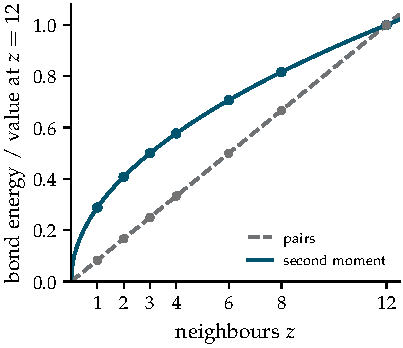
\includegraphics{ch08_potentials/manybody}
\caption{The bond energy of an atom with $z$ neighbours, as a fraction of
its value at $z = 12$: proportional to $z$ for a pair potential
(dashed), and to $\sqrt{z}$ for the second-moment model (teal), at a pair
of atoms (1), a chain (2), a graphite layer (3), diamond (4), simple
cubic (6), body-centred cubic lithium (8) and close-packed metals (12).}
\label{fig:pe-manybody}
\end{figure}

The forces follow from the chain rule. The square root couples every
neighbour of $i$: moving atom $k$ changes $\rho_i$ through the term
$r_{ik}$, and $\sqrt{\rho_i}$ changes by $\frac12\rho_i^{-1/2}$ times that.
The force on an atom therefore depends on the neighbours of its
neighbours, and is no longer a sum of forces along pairs with fixed
strengths. The forces still add to zero and exert no total torque, because $U$
depends only
on distances and so does not change when all the atoms are moved or
turned together (\cref{sec:ha-noether}); the function
\texttt{second\_moment} of \texttt{mdlab} computes it, and its test
checks it against central differences.

The embedded-atom method generalises \cref{eq:pe-second-moment}: the
energy of atom $i$ is $\mathcal{F}(\bar\rho_i) + \frac12\sum_j\varphi
(r_{ij})$, with
$\bar\rho_i$ the density of the electrons, their charge per unit volume,
that its neighbours produce where it sits and $\mathcal{F}$, the embedding energy, a function fitted to measurements or
to calculations\cite{DawBaskes1984}. The second-moment model is the case
$\mathcal{F}(\bar\rho) = -\sqrt{\bar\rho}$, with $\bar\rho_i = \rho_i$ and
$\varphi(r) = 2A\,\mathrm{e}^{-\eta(r/r_0 - 1)}$, the 2 making up for the
$\frac12$.

\subsection*{Carbon and the order of a bond}

Carbon forms directional bonds, three to a layer in graphite and four in
diamond, and its bonds too weaken as they multiply. Tersoff's potential
writes the energy as a sum over bonds, $\frac12\sum_i\sum_{j\ne i}f_{\mathrm
c}(r_{ij})\bigl[f_{\mathrm R}(r_{ij}) - b_{ij}f_{\mathrm A}(r_{ij})
\bigr]$, with a repulsion $f_{\mathrm R}$, an attraction $f_{\mathrm A}$,
a smooth cutoff $f_{\mathrm c}$, and a bond order $b_{ij}$ that falls as
atom $i$ gains other neighbours, depending also on the angles between its
bonds\cite{Tersoff1988,Tersoff1988carbon}. The reactive bond-order potential of Brenner and
co-workers extends this to hydrocarbons and describes the strong bonds
within a graphite layer\cite{Brenner2002}. It has no interaction between
the layers, which are held together by the weak attraction between
neutral atoms; a version adds a Lennard-Jones term for
it\cite{Stuart2000}. Lithium between the layers of graphite needs, in
addition, lithium-carbon and lithium-lithium interactions, and models
fitted for this are among the machine-learned potentials planned for the
continuation of Part~V.

\begin{keyidea}
In metals and in carbon the strength of a bond falls as an atom's bonds
multiply. The second-moment model, with bond energy $-\sqrt{\rho_i}$,
makes the bond energy grow as $\sqrt{z}$; the embedded-atom method and
bond-order potentials refine the same idea. Their forces couple the
neighbours of neighbours but still add to zero and exert no total
torque.
\end{keyidea}

\notebook{08}{the second-moment model: bonds against neighbours}

\begin{selfcheck}
In the second-moment model, by what factor is one bond of an atom in a
chain ($z = 2$) stronger than one bond in close-packed metal?
\end{selfcheck}

%=============================================================================!
% 8.7  BONDED FORCE FIELDS                                                    !
%=============================================================================!
\section{Bonded force fields}
\label{sec:pe-bonded}

The solvents of a lithium-ion battery's electrolyte are small organic
molecules, carbonates such as ethylene carbonate, a ring of five atoms,
and chains such as dimethyl carbonate. While no reaction takes place, each
atom of a molecule keeps the same bonded partners, and its energy can be
written as a sum of terms for the bonds, the angles between bonds and the
twists about them, with the interactions of atoms farther apart, in the
same molecule or in different ones, added as pairs.
This section sets out that form, called a force field, and the one new
piece of geometry it needs, the dihedral angle.

\subsection*{The terms}

In the all-atom form, in which every hydrogen is a site of its own, of
the force field OPLS (Optimized Potentials for Liquid Simulations) of
Jorgensen and co-workers\cite{Jorgensen1996},
\begin{equation}
   \begin{aligned}
   U &= \sum_{\text{bonds}}\kappa_r(r - r_{\mathrm{eq}})^2
   + \sum_{\text{angles}}\kappa_\theta(\theta - \theta_{\mathrm{eq}})^2
   + \sum_{\text{dihedrals}}\sum_{n=1}^{3}\frac{\kappa_n}{2}\bigl[1 + (-1)^{n+1}
   \cos n\psi\bigr]\\
   &\quad + \sum_{i<j}f_{ij}\Bigl[\frac{k_{\mathrm e}q_iq_j}{r_{ij}}
   + 4\varepsilon_{ij}\Bigl(\frac{\sigma_{ij}^{12}}{r_{ij}^{12}}
   - \frac{\sigma_{ij}^6}{r_{ij}^6}\Bigr)\Bigr] .
   \end{aligned}
   \label{eq:pe-opls}
\end{equation}
The first sum holds each bond near its length $r_{\mathrm{eq}}$ by a
spring; $\kappa_r$ is half the stiffness $k$ of the spring energy $\frac12
kx^2$ (\cref{sec:en-varying}), since the factor $\frac12$ is absorbed into
it. The second holds each angle
$\theta$ between two bonds at an atom near $\theta_{\mathrm{eq}}$, as the
three atoms of \cref{fig:ha-noether}(a) were held, with $\kappa_\theta$
half the angular stiffness for the same reason. The third gives the
energy of a twist $\psi$ about each bond as a short series of cosines,
written out $\frac12\kappa_1(1 + \cos\psi) + \frac12\kappa_2(1 - \cos2\psi)
+ \frac12\kappa_3(1 + \cos3\psi)$ with constants $\kappa_n$, and
the last adds the Coulomb energy of charges $q_i$ placed on the atoms
(\cref{sec:pe-coulomb}) and a Lennard-Jones energy, for every pair. The
factor $f_{ij}$ is 0 for atoms joined by one bond or two, whose
interaction the bond and angle terms already describe, $\frac12$ for
atoms three bonds apart, and 1 for all others, including every pair in
different molecules. Each constant depends on the kinds of atom involved,
and a force field is a table of them, fitted to calculations of the
electrons and to measured properties of liquids.

\subsection*{The dihedral angle}

Four atoms bonded in a chain, $a$--$b$--$c$--$d$, can twist about the
middle bond $b$--$c$ (\cref{fig:pe-dihedral}). The twist is measured by
the angle between the plane of $a$, $b$, $c$ and the plane of $b$, $c$,
$d$, seen along the middle bond. Each plane is fixed by the arrow at right
angles to it, which the cross product of two arrows in the plane gives
(\cref{sec:ro-cross}). With $\vb{b}_1 = \vb{r}_b - \vb{r}_a$, $\vb{b}_2 =
\vb{r}_c - \vb{r}_b$ and $\vb{b}_3 = \vb{r}_d - \vb{r}_c$ along the
three bonds,
\begin{equation*}
   \vb{n}_1 = \vb{b}_1\times\vb{b}_2 , \qquad
   \vb{n}_2 = \vb{b}_2\times\vb{b}_3
\end{equation*}
are at right angles to the first and second planes. Seen along
$\vb{b}_2$, the two planes appear as lines from the middle bond towards
$a$ and towards $d$, and $\psi$ is the angle between them. The part of
$\vb{b}_1$ along $\vb{b}_2$ drops out of $\vb{n}_1$, since $\vb{b}_2\times
\vb{b}_2 = \vb{0}$, and the part left points from $a$ towards the bond, so
$\vb{n}_1$ is $\vb{b}_2$ crossed with an arrow from the bond towards $a$;
likewise $\vb{n}_2$ is $\vb{b}_2$ crossed with an arrow from the bond
towards $d$. Each is its line turned through a right angle about
$\vb{b}_2$, the same way for both, so the angle between them is $\psi$,
and by the dot product
\begin{equation}
   \cos\psi = \frac{\vb{n}_1\cdot\vb{n}_2}{\lvert\vb{n}_1\rvert\,
   \lvert\vb{n}_2\rvert} .
   \label{eq:pe-dihedral}
\end{equation}
The cosine does not tell a twist one way from the same twist the other
way. The cross product $\vb{n}_1\times\vb{n}_2$ is along $\vb{b}_2$, the
one direction at right angles to both, pointing along $\vb{b}_2$ or
against it according to the sense of the twist, so the sign of
$(\vb{n}_1\times\vb{n}_2)\cdot\vb{b}_2$ gives the sign of $\psi$, which
then runs from $-\pi$ to $\pi$; $\psi$ is positive when, seen from $b$
looking towards $c$, the bond to $a$ turns clockwise to reach the bond to
$d$. For a flat zigzag, $a$ and $d$ on
opposite sides of the middle bond, $\vb{n}_1$ and $\vb{n}_2$ point in
opposite directions and $\psi = \ang{180}$, the arrangement called
trans; with $a$ and $d$ on the same side, $\psi = 0$, called cis. The
function \texttt{dihedral\_angle} of \texttt{mdlab} computes $\psi$ in
this way.

\begin{figure}[htb]
\centering
\begin{tikzpicture}[line cap=round, line join=round, scale=1.2,
   atom/.style={circle, fill=black, inner sep=1.6pt},
   arr/.style={-{Stealth[length=5pt]}, line width=0.8pt, accent}]
   \draw[line width=1pt] (0,0) -- (90:1.3) node[atom, label={above:$a$}] {};
   \draw[line width=1pt] (0,0) -- (-30:1.3) node[atom, label={right:$d$}] {};
   \node[atom, label={left:{$b$ in front of $c$}}] at (0,0) {};
   \draw[arr] (0,0) -- (0:1.0) node[right] {$\vb{n}_1$};
   \draw[arr] (0,0) -- (240:1.0) node[below] {$\vb{n}_2$};
   \draw[black!50] (90:0.5) arc[start angle=90, end angle=-30, radius=0.5];
   \node at (45:0.72) {$\psi$};
\end{tikzpicture}
\caption{Four atoms bonded in a chain, seen along the middle bond with
$b$ in front of $c$. The planes of $a$, $b$, $c$ and of $b$, $c$, $d$ are
seen edge-on as the lines towards $a$ and $d$, at the dihedral angle
$\psi$; $\vb{n}_1$ and $\vb{n}_2$ are those lines turned through a right
angle the same way, so they meet at the same angle.}
\label{fig:pe-dihedral}
\end{figure}

\begin{keyidea}
A force field writes the energy of molecules as springs for bonds and
angles, a cosine series for each twist, and Coulomb and Lennard-Jones
energies between atoms more than two bonds apart. The twist is the
dihedral angle between the two planes of a chain of four atoms, found
from two cross products.
\end{keyidea}

\notebook{08}{twist a chain of four atoms and watch its torsion energy}

\begin{selfcheck}
In \cref{eq:pe-opls}, which values of $\psi$ make the $\kappa_1$ and the
$\kappa_3$ terms smallest, when both constants are positive?
\end{selfcheck}

%=============================================================================!
% 8.8  LONG-RANGE ELECTROSTATICS                                              !
%=============================================================================!
\section{Charges and the slow decay of \texorpdfstring{$1/r$}{1/r}}
\label{sec:pe-coulomb}

Ions in an electrolyte, the charged atoms of a crystal such as rock salt
and the charges placed on the atoms of a force field interact by
Coulomb's law. Two charges
$q_i$ and $q_j$, in units of the elementary charge $e$, the charge of a
proton (an electron carries $-e$, and an ion is an atom that has lost or
gained electrons), at a distance $r$ have the energy
\begin{equation}
   \varphi_{\mathrm C}(r) = \frac{k_{\mathrm e}\,q_iq_j}{r} ,
   \qquad k_{\mathrm e} = \frac{e^2}{4\pi\epsilon_0} = \SI{14.3996}{\electronvolt
   \angstrom} ,
   \label{eq:pe-coulomb}
\end{equation}
where $\epsilon_0$ is the electric constant; $k_{\mathrm e}$ is computed from its
value in \texttt{mdlab.units}. This section shows that this energy cannot be
cut off as the earlier ones were.

\subsection*{A slow decay}

Two opposite unit charges at \SI{1.5639}{\angstrom}, the bond length of
LiF (\cref{sec:ro-molecules}), have $-14.3996/1.5639 =
\SI{-9.21}{\electronvolt}$; at \SI{10}{\angstrom} they still have
$\SI{-1.44}{\electronvolt}$, where two argon atoms have
$\SI{-6.4e-5}{\electronvolt}$. Take an ion inside a large region filled with ions at the number density
$n$, that is $n$ ions in each unit of volume. The ions at distances between $r$ and $r + \Delta r$ fill a
shell of area $4\pi r^2$ and thickness $\Delta r$, so there are about
$4\pi r^2n\,\Delta r$ of them, a number that grows as $r^2$. Each
contributes an energy of size $k_{\mathrm e}/r$, so the shell as a whole contributes
an amount of size $4\pi k_{\mathrm e}n\,r\,\Delta r$, which grows with $r$. For a
Lennard-Jones attraction the same shell contributes $4\pi r^2n\,\Delta
r\times r^{-6}$, falling as $r^{-4}$, and the far shells hardly matter;
for charges, every shell counts more than the last, and only the
cancellation between positive and negative ions keeps the total finite.

\subsection*{A sum that depends on its order}

Rock salt, NaCl, shows what this means. Its ions sit on a cubic grid of
spacing $d$, the sign of the charge alternating from each site to its
neighbours, so the ion at $(a, b, c)d$, with $a$, $b$, $c$ integers, positive,
negative or zero,
carries the charge $(-1)^{a+b+c}$ relative to the ion at the origin. The
energy of the ion at the origin with all the others is $-\mathcal{M}k_{\mathrm e}/d$, with the Madelung
constant
\begin{equation*}
   \mathcal{M} = -\sum_{(a,b,c)\ne(0,0,0)}\frac{(-1)^{a+b+c}}{\sqrt{a^2 + b^2 + c^2}} .
\end{equation*}
\Cref{fig:pe-madelung} adds up this sum in two orders. Over the ions
inside a growing sphere, the partial sums do not settle, out to $12d$: the six nearest
ions alone give the partial sum 6, adding the twelve next give $-2.49$, and between
radii $6d$ and $12d$ the sums swing between $-10.3$ and $+14.7$, because
each new shell of ions has a net charge of its own. Over the ions inside a
growing cube, with the ions on its faces, edges and corners counted with
the fractions $\frac12$, $\frac14$ and $\frac18$ of a small cube of side
$d$ around each that lie inside, every cube is neutral: the weighted
charge is a product of three equal sums, one along each axis, each zero,
as $-\frac12 + 1 - \frac12 = 0$ for the smallest cube. The sums settle
quickly, to 1.747567 at a half-side of $12d$, within $2\times10^{-6}$ of
the limit 1.747565\cite{Evjen1932}. The answer depends on the order in
which the terms are added. That cannot happen when the sizes of the
terms, all taken positive, add up to a finite total; here they do not,
since the sizes in one shell add up to an amount that grows as $r$.
Physically, the arrangement of charge at the surface of the
region summed over affects the energy of every ion inside it. For a crystal of this kind with a spacing $d =
\SI{2.82}{\angstrom}$, the electrostatic energy of one ion with all the
others is $-1.7476\times14.3996/2.82 = \SI{-8.92}{\electronvolt}$.

\begin{figure}[htb]
\centering
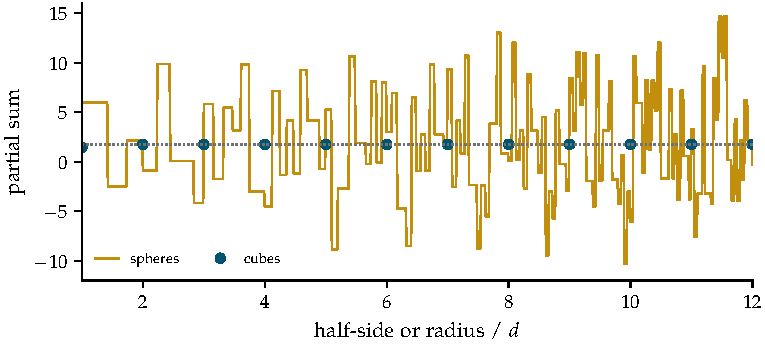
\includegraphics{ch08_potentials/madelung}
\caption{The Madelung sum of rock salt over the ions inside a growing
sphere (ochre), which never settles, and inside a growing neutral cube
(teal dots), which settles to 1.7476 (dotted), against the radius or
half-side in units of the nearest-neighbour distance $d$.}
\label{fig:pe-madelung}
\end{figure}

A cutoff therefore cannot be applied to charges as it was to the
Lennard-Jones energy: whatever its radius, the charge inside it is not
zero in general and the energy depends on where it falls. Electrolytes,
full of ions, and electrodes, whose surfaces carry charge, need the
electrostatic energy of an infinite, periodic arrangement of charges
summed correctly. Chapter~10, once periodic boxes are in place, derives
the Ewald method, one way of doing that.

\begin{keyidea}
The Coulomb energy $k_{\mathrm e}q_iq_j/r$ falls so slowly that each shell of
charges matters more than the last, and the sum for a crystal of ions
depends on the order in which its terms are added, which sets the charge
at the surface of the region summed. Charges cannot be cut off like a
Lennard-Jones energy, and periodic systems need a sum built for them,
such as the Ewald sum of Chapter~10.
\end{keyidea}

\notebook{08}{sum the charges of rock salt over spheres and cubes}

\begin{selfcheck}
How many ions lie at the distance $\sqrt2\,d$ from an ion in rock salt,
and what is their charge relative to it?
\end{selfcheck}

%=============================================================================!
% 8.S  WHAT WE NOW HAVE                                                       !
%=============================================================================!
\unnumbered{What we now have}

The potential energy on which atoms move is the energy of their electrons,
settled at each arrangement of the nuclei, plus the repulsion of the
nuclei: the potential energy surface of Born and Oppenheimer. The dense eigensolver considered here has a cost that grows as the cube
of its matrix size, motivating cheaper models of the energy. Treating the nuclei
themselves as classical is good when the quantum step $\hbar\omega$ of
their vibrations is small beside $\kB T$, which holds for heavy atoms and
slow motions and fails for the stretches of bonds to hydrogen.

The simplest models add up pair potentials, the Lennard-Jones, Morse and
exp-6 shapes, whose forces are computed once per pair and applied with
opposite signs, with the virial $\mathcal{W} = -\sum r_{ij}\varphi'(r_{ij})$
alongside; in reduced units every Lennard-Jones substance obeys the same
equations. Every force routine is checked against central differences of
its energy, at a step near the cube root of the machine epsilon times the
length scale.

A cutoff must take both energy and force smoothly to zero:
truncation breaks the conservation of energy, shifting leaves a jump in
the force that an adaptive solver follows only with far shorter steps,
and switching or a smooth envelope removes both jumps.

In metals and carbon the strength of a bond
falls as an atom's bonds multiply, which the second-moment model, the
embedded-atom method and bond-order potentials describe; molecules are
described by force fields of bonds, angles, dihedral twists and
non-bonded pairs; and the Coulomb energy of charges falls so slowly that
its sum depends on its order.

Chapter~9 uses these forces to follow the motion step by step, and
Chapter~10 builds a complete simulation of atoms in a periodic box, with
neighbour lists for the cutoffs and the Ewald sum for the charges.

%=============================================================================!
% 8.A  ANSWERS TO THE CHECKS                                                  !
%=============================================================================!
\unnumbered{Answers to the checks}
\label{sec:pe-answers}

\answerto{sec:pe-origin}The size grows by a factor of 4, so the time by
$4^3 = 64$: about \SI{6.4}{\second}.

\answerto{sec:pe-classical}No. Its quantum step is $\hbar\omega =
2\pi\hbar c\,\tilde\nu = 1.2398\times10^{-4}\times3000 = \SI{0.372}{\electronvolt}$,
14.4 times $\kB T = \SI{0.02585}{\electronvolt}$.

\answerto{sec:pe-pairs}$\tau = \sigma\sqrt{m/\varepsilon}$. Krypton's
$\sigma$ is larger by a factor $3.6/3.4 = 1.06$ and its $m/\varepsilon$ by
$(83.8/39.948)/(160/120) = 1.57$, whose square root is 1.25, so its
$\tau$ is about 1.33 times argon's, longer: it is heavier, and the extra
depth of its well does not make up for that.

\answerto{sec:pe-forces}At $r = \sigma$, closer than the minimum at
$1.12\sigma$, the pair repels, $\varphi'(\sigma) = 4\varepsilon(-12 + 6)/
\sigma = -24\varepsilon/\sigma < 0$, so $\mathcal{W} = -\sigma\varphi'(\sigma) =
+24\varepsilon$: positive.

\answerto{sec:pe-cutoffs}$\lvert\varphi(2.5\sigma)\rvert = 0.0163\times
\SI{0.01034}{\electronvolt} = \SI{1.69e-4}{\electronvolt}$ per crossing.

\answerto{sec:pe-manybody}Each bond is worth $\xi/\sqrt{z}$, so the ratio
is $\sqrt{12}/\sqrt2 = \sqrt6 = 2.45$.

\answerto{sec:pe-bonded}$1 + \cos\psi$ is least, 0, at $\psi = \ang{180}$;
$1 + \cos3\psi$ is 0 where $\cos3\psi = -1$, that is $3\psi = \ang{180}$,
\ang{540} or $-\ang{180}$, so $\psi = \ang{60}$, \ang{180} or $-\ang{60}$.
Both are least at \ang{180}, the trans arrangement.

\answerto{sec:pe-coulomb}The sites $(a, b, c)$ with $a^2 + b^2 + c^2 = 2$
have two of $a$, $b$, $c$ equal to $\pm1$ and one 0: three choices of the
zero and four of the signs, 12 ions. Their $a + b + c$ is even, so they
carry the same charge as the ion at the origin.

%=============================================================================!
% 8.E  EXERCISES                                                              !
%=============================================================================!
\unnumbered{Exercises}
\label{sec:pe-exercises}

The exercises run from questions of understanding, through calculations,
to short derivations marked `show that'. Full solutions are in
\hyperref[sec:pe-solutions]{`Solutions to the exercises'} at the end of
the book, and Notebook~08 checks every numerical answer.

\begin{exercise}[fast electrons]
\label{ex:pe-ratio}
With the same stiffness, how many times faster than a lithium atom of
\SI{6.94}{amu} does an electron vibrate? (An electron's mass is
\SI{5.486e-4}{amu}.)
\end{exercise}

\begin{exercise}[when quantum steps matter]
\label{ex:pe-quantum}
At what temperature is $\kB T$ equal to the quantum step $\hbar\omega$ of
the model lithium hollow of \cref{sec:pe-classical}, and of the O--H
stretch?
\end{exercise}

\begin{exercise}[the strongest pull]
\label{ex:pe-lj-pull}
Show that two Lennard-Jones atoms attract most strongly at $r =
(26/7)^{1/6}\sigma = 1.2445\,\sigma$, and find that greatest pull.
\end{exercise}

\begin{exercise}[the lowered Morse well]
\label{ex:pe-morse}
Show that $\varphi_{\mathrm M}(r) = D(\mathrm{e}^{-2a(r-r_0)} -
2\mathrm{e}^{-a(r-r_0)})$ has its minimum $-D$ at $r_0$ and the stiffness
$2Da^2$ there.
\end{exercise}

\begin{exercise}[the exp-6 form]
\label{ex:pe-exp6}
Show that, for $\alpha > 7$, the Buckingham potential with $A = 6\varepsilon\,\mathrm{e}^
{\alpha}/(\alpha - 6)$, $\rho = r_{\mathrm m}/\alpha$ and $C =
\alpha\varepsilon r_{\mathrm m}^6/(\alpha - 6)$ has its minimum
$-\varepsilon$ at $r_{\mathrm m}$.
\end{exercise}

\begin{exercise}[an argon pair]
\label{ex:pe-argon}
Two argon atoms vibrate about the Lennard-Jones minimum with the reduced
mass $m/2$ (\cref{sec:os-bodies}). Find the period of small vibrations in
units of $\tau$ and in femtoseconds, and how many steps of $0.005\tau$ it
spans.
\end{exercise}

\begin{exercise}[no total force]
\label{ex:pe-third}
Show from \cref{eq:pe-pair-force} that the forces of any pair potential
add to zero.
\end{exercise}

\begin{exercise}[the virial of a pair]
\label{ex:pe-virial}
Find the virial of two Lennard-Jones atoms at $r = 1.5\sigma$, and say for
which distances it is positive.
\end{exercise}

\begin{exercise}[the best step]
\label{ex:pe-best-step}
For the twelve atoms of \cref{fig:pe-fd}, $\lvert U\rvert =
10.75\varepsilon$; take $\lvert U'''\rvert \approx 10^4\,\varepsilon/
\sigma^3$. Use \cref{eq:pe-fd-error} to estimate the best step.
\end{exercise}

\begin{exercise}[a one-sided difference]
\label{ex:pe-forward}
Show that the forward difference $[U(x + h) - U(x)]/h$ has an error of
about $\frac12 h\lvert U''\rvert + \epsilon_{\mathrm m}\lvert U\rvert/h$,
and that its best step is of order $\sqrt{\epsilon_{\mathrm m}}$ times
the length on which $U$ changes and its least error of order
$\sqrt{\epsilon_{\mathrm m}}$ times the forces, much worse than for
central differences.
\end{exercise}

\begin{exercise}[the switching function]
\label{ex:pe-switch}
Show that $S(x) = 1 - 10x^3 + 15x^4 - 6x^5$ has $S(0) = 1$, $S(1) = 0$,
and its first and second derivatives zero at $x = 0$ and $x = 1$.
\end{exercise}

\begin{exercise}[TrajCast's envelope]
\label{ex:pe-envelope}
Show that the envelope $u(x) = 1 - 28x^6 + 48x^7 - 21x^8$, the case $p = 6$
of \cref{sec:pe-cutoffs}, has $u(1) = 0$ and $u'(1) = u''(1) = 0$.
\end{exercise}

\begin{exercise}[the energy beyond the cutoff]
\label{ex:pe-tail}
Atoms beyond $r_{\mathrm c}$ are spread evenly at the number density
$n$, the number of atoms per unit volume.
Show that the Lennard-Jones energy per atom that a cutoff leaves out is
$\frac83\pi n\varepsilon\sigma^3[\frac13(\sigma/r_{\mathrm c})^9 -
(\sigma/r_{\mathrm c})^3]$, and evaluate it for $n = 0.8\sigma^{-3}$ and
$r_{\mathrm c} = 2.5\sigma$.
\end{exercise}

\begin{exercise}[counting crossings]
\label{ex:pe-crossings}
In \cref{fig:pe-cutoff}(c) the truncated energy rises by up to
$0.49\varepsilon$ above its starting value. How many fewer pairs lie
inside the cutoff than at the start?
\end{exercise}

\begin{exercise}[the force of a square root]
\label{ex:pe-sqrt-force}
Show that the bond energy $-\sqrt{\rho_i}$ of \cref{eq:pe-second-moment}
acts on atom $k \ne i$ with the force $\frac12\rho_i^{-1/2}\,\grad_k
\rho_i$, and write $\grad_k\rho_i$ out.
\end{exercise}

\begin{exercise}[a vacancy]
\label{ex:pe-vacancy}
In a crystal where every atom has $z$ neighbours at the same distance,
an atom is removed from inside and put back elsewhere on the surface of
the crystal; putting it there gains, on average, the energy that holds
one atom in the crystal.
Counting only the bond energy, show that a pair potential makes the
energy of the vacancy equal to that energy, and that the second-moment
model makes it $z(1 - \sqrt{1 - 1/z})$ times it; evaluate this for $z =
12$.
\end{exercise}

\begin{exercise}[a right-angled twist]
\label{ex:pe-dihedral}
Find the dihedral angle of the atoms at $(1, 0, 0)$, $(0, 0, 0)$, $(0, 0,
1)$ and $(0, 1, 1)$ (in \AA), and the torsion energy of
\cref{eq:pe-opls} there with $\kappa_1 = 0.1$, $\kappa_2 = 0.02$ and
$\kappa_3 = \SI{0.05}{\electronvolt}$.
\end{exercise}

\begin{exercise}[as weak as heat]
\label{ex:pe-bjerrum}
At what distance is the Coulomb energy of two unit charges in vacuum
equal to $\kB T$ at \SI{300}{\kelvin}?
\end{exercise}

\begin{exercise}[the first shells]
\label{ex:pe-shells}
Count the ions of rock salt at distances $\sqrt3\,d$ and $2d$ from an ion,
give their charges, and find the sphere sums for $\mathcal{M}$ up to radii $d$,
$\sqrt2\,d$, $\sqrt3\,d$ and $2d$.
\end{exercise}

\begin{exercise}[the smallest neutral cube]
\label{ex:pe-cube}
Find by hand the cube sum for $\mathcal{M}$ with half-side $d$, counting the ions on
the faces, edges and corners with weights $\frac12$, $\frac14$ and
$\frac18$.
\end{exercise}


%=============================================================================!
% CHAPTER 9  INTEGRATING THE EQUATIONS OF MOTION                              !
%=============================================================================!
\chapter{Integrating the equations of motion}
\label{ch:integrators}

%=============================================================================!
% 9.0  CHAPTER OPENING                                                        !
%=============================================================================!
Once the forces are known, a simulation must use them to advance the
positions and velocities. The computer cannot follow every instant: it
computes a sequence of states separated by a finite time step. Chapter~2
used the forward Euler method, Chapter~3 used a more accurate solver, and
Chapter~7 showed that two methods with similar errors over one step can
behave quite differently over a long run.

This chapter develops velocity Verlet, a method widely used in molecular
dynamics. Its construction from Taylor series gives the error of a step;
its construction from kicks and drifts explains its reversibility and
preservation of phase-space volume. For a spring it keeps a slightly
different energy exactly, which lets us derive both its energy error and
its stability limit. These results give a practical way to choose the
step for a molecule, including the water example left open in
Chapters~1, 2 and~4. Long runs then test the method against RK4 and show
why the smooth forces of Chapter~8 matter. Chapter~10 assembles these
parts into a complete simulation in a periodic box.

%=============================================================================!
% 9.1  STEPS AND THEIR ERRORS                                                 !
%=============================================================================!
\section{Steps and their errors}
\label{sec:in-steps}

A method of computing motion is a step map (\cref{sec:ha-symplectic}): it
takes the positions and velocities at a time $t$ and returns them at $t
+ \dt$. Applied over and over it produces the motion at the times $\dt$,
$2\dt$, $3\dt$, \dots, and the question is how far that computed motion
strays from the true one. This section measures it for the simplest
method and defines the order of a method, the number that says how fast
its error shrinks as the step is shortened.

\subsection*{The forward Euler method again}

\Cref{sec:ne-equations} advanced a motion by holding the velocity and the
acceleration at their values at the start of each step:
\begin{equation*}
   x_{n+1} = x_n + \dt\,v_n , \qquad v_{n+1} = v_n + \dt\,a(x_n) ,
\end{equation*}
where $x_n$ and $v_n$ are the computed position and velocity after $n$
steps, at the time $t_n = n\dt$. The Taylor series of the true position
over one step (\cref{sec:mo-taylor}), and the same series for the
velocity, whose derivatives are $\dot{v} = a$ and $\ddot{v} = \dot{a}$, the
rate of change of the acceleration,
\begin{align*}
   x(t + \dt) &= x(t) + v(t)\,\dt + \tfrac12 a(t)\,\dt^2 + \order{\dt^3} ,\\
   v(t + \dt) &= v(t) + a(t)\,\dt + \tfrac12\dot{a}(t)\,\dt^2
   + \order{\dt^3} ,
\end{align*}
show what one step misses: started from the true state, the computed
position is wrong by $\frac12 a\dt^2$ and the computed velocity by
$\frac12\dot{a}\dt^2$, each plus smaller terms. The error made in one step
from a correct start is called the local error; for the forward Euler
method it is of order $\dt^2$.

\subsection*{From one step to a whole run}

To follow the motion for a fixed time $t_{\mathrm f}$ needs $t_{\mathrm
f}/\dt$ steps. Each makes a local error of order $\dt^2$, and each error is
carried forward by the later steps. For a smooth force, an error carried
through one step grows by a factor of at most $1 + c\,\dt$, with $c$ a
bound on how fast the rates of change depend on the state, so through all
the later steps by at most
\begin{equation*}
   (1 + c\,\dt)^{t_{\mathrm f}/\dt} \le \bigl(\mathrm{e}^{c\,\dt}
   \bigr)^{t_{\mathrm f}/\dt} = \mathrm{e}^{ct_{\mathrm f}} ,
\end{equation*}
since $1 + y \le 1 + y + \frac12y^2 + \dotsb = \mathrm{e}^y$ for $y \ge
0$. This factor depends on $t_{\mathrm f}$ and on the force but not on
$\dt$, and the error at $t_{\mathrm f}$ is at most it times the sum of the
local errors\cite{LeimkuhlerMatthews2015}: $(t_{\mathrm f}/\dt)
\times\order{\dt^2} = \order{\dt}$. A method whose error over a fixed
time, its global error, is of order $\dt$ is said to be of order 1, one
whose global error is of order $\dt^2$ of order 2, and so on. For a method
that computes each state from the one before it alone, as the forward
Euler method does, the local error is one power of $\dt$ higher than the
global error. The forward Euler method is of order 1: halving the step
halves the error at a given time, as \cref{sec:ne-equations} found.

\Cref{fig:in-orders} measures this for the pendulum of Chapter~7, $H =
p^2/(2mL^2) + mgL(1 - \cos\theta)$, with energies in units of $mgL$ and
times in units of $\sqrt{L/g}$, which amounts to setting $m = L = g = 1$,
as the reduced units of \cref{sec:pe-pairs} do for atoms. Writing $q$ for
the angle, $H = p^2/2 + 1 - \cos q$ and $\ddot{q} = -\sin q$. Started at
the angle $q = 1$ with the momentum $p = 0.5$, the error of the angle
after a time of 4 falls with the step along a line of slope 1.03 on
logarithmic axes (\cref{sec:mo-taylor}), and its error after a single
step along a line of slope 2.01. The figure also shows
the two methods of the next sections, whose errors fall much faster.

\begin{figure}[htb]
\centering
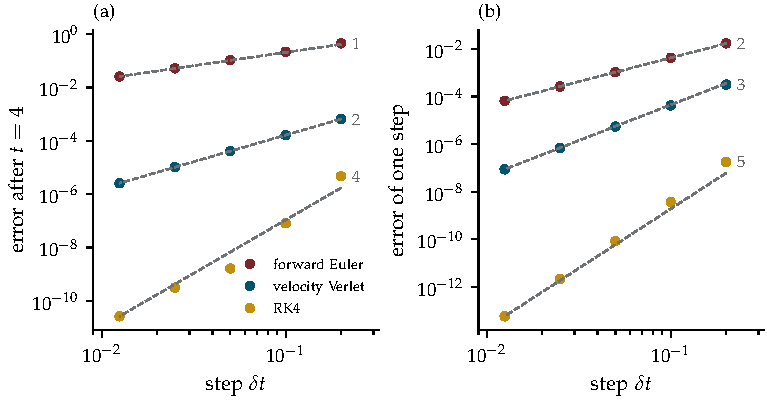
\includegraphics{ch09_integrators/orders}
\caption{The errors of three methods for the pendulum $H = p^2/2 + 1 -
\cos q$ in reduced units, started at $q = 1$, $p = 0.5$, against the step
$\dt$, on logarithmic axes. (a) The error of the angle after a time of 4,
with lines of slope 1, 2 and 4 (dashed). (b) The error of the angle after
one step from the same start, with lines of slope 2, 3 and 5.}
\label{fig:in-orders}
\end{figure}

\begin{keyidea}
A method's local error is the error of one step from a correct start.
For a method that steps from the present state alone, the errors of the
$t_{\mathrm f}/\dt$ steps add up over a fixed time to a global error with
one power of $\dt$ fewer, and that power is the order of the method: the
forward Euler method, with local and global errors of order $\dt^2$ and
$\dt$, is of order 1.
\end{keyidea}

\begin{selfcheck}
Halving the step of a method divides its error at a given time by 4.
What is its order, and how does its local error depend on $\dt$?
\end{selfcheck}

%=============================================================================!
% 9.2  THE VERLET METHOD                                                      !
%=============================================================================!
\section{The Verlet method}
\label{sec:in-verlet}

Verlet's method, which Verlet introduced in 1967 for his simulations of a
liquid of Lennard-Jones atoms\cite{Verlet1967}, gains a whole order over the forward
Euler method at the same cost of one force evaluation per step. This
section derives it from the Taylor series, writes it in the form that
simulations use, and checks its order.

\subsection*{Positions from two Taylor series}

The Taylor series of the motion a step ahead and a step behind are
\begin{align*}
   x(t + \dt) &= x + v\,\dt + \tfrac12 a\,\dt^2 + \tfrac16\dot{a}\,\dt^3
   + \tfrac1{24}\ddot{a}\,\dt^4 + \order{\dt^5} ,\\
   x(t - \dt) &= x - v\,\dt + \tfrac12 a\,\dt^2 - \tfrac16\dot{a}\,\dt^3
   + \tfrac1{24}\ddot{a}\,\dt^4 + \order{\dt^5} ,
\end{align*}
with $x$, $v$, $a$ and the derivatives of $a$ taken at $t$; the second is
the first with $-\dt$ in place of $\dt$, which changes the sign of every
odd power. Adding them, the odd powers cancel, the terms in $\dt^5$
within $\order{\dt^5}$ among them, so the remainder is of order $\dt^6$:
\begin{align*}
   x(t + \dt) + x(t - \dt) &= 2x + a\,\dt^2 + \tfrac1{12}\ddot{a}\,\dt^4
   + \order{\dt^6}
   && \text{$\tfrac1{24} + \tfrac1{24} = \tfrac1{12}$}\\
   x(t + \dt) &= 2x(t) - x(t - \dt) + \dt^2a(t) + \order{\dt^4}
   && \text{subtracting $x(t - \dt)$,}
\end{align*}
the term in $\dt^4$ joining the remainder.
Dropping the last term gives the Störmer--Verlet method,
\begin{equation}
   x_{n+1} = 2x_n - x_{n-1} + \dt^2\,a(x_n) ,
   \label{eq:in-stormer}
\end{equation}
which advances the positions with an error of order $\dt^4$ in one step
from two correct positions, using only the force at the present position.
Its global error is nevertheless of order $\dt^2$, as for velocity Verlet
below. An error made in one position, with the one before it correct,
changes the difference between successive positions, which every later
step carries forward, so over a fixed time each local error grows by a
factor of order $t_{\mathrm f}/\dt$, and the $t_{\mathrm f}/\dt$ of them
give $(t_{\mathrm f}/\dt)^2\times\order{\dt^4} = \order{\dt^2}$. The rule
of \cref{sec:in-steps} that relates the two orders holds only for methods
that step from the present state alone. The velocities do not appear, but
can be recovered by the central difference of \cref{sec:mo-atoms}, $v_n =
(x_{n+1} - x_{n-1})/(2\dt)$, with an error of order $\dt^2$.

\subsection*{Velocity Verlet}

Simulations need the velocities at the same times as the positions, for
the kinetic energy and to start a run from a state. Expanding the
position and the velocity over one step,
\begin{align*}
   x(t + \dt) &= x + v\,\dt + \tfrac12 a\,\dt^2 + \order{\dt^3} ,\\
   v(t + \dt) &= v + a\,\dt + \tfrac12\dot{a}\,\dt^2 + \order{\dt^3} .
\end{align*}
The derivative $\dot{a}$ is not known, but $a(t + \dt) = a + \dot{a}\,\dt
+ \order{\dt^2}$, so $\dot{a}\,\dt = a(t + \dt) - a(t) + \order{\dt^2}$,
and putting this into the velocity series,
\begin{align*}
   v(t + \dt) &= v + a\,\dt + \tfrac12\bigl[a(t + \dt) - a(t)\bigr]\dt +
   \order{\dt^3}\\
   &= v + \tfrac12\bigl[a(t) + a(t + \dt)\bigr]\dt + \order{\dt^3} :
\end{align*}
the velocity changes by the average of the accelerations at the two ends
times the step. Dropping the error terms gives the velocity Verlet
method\cite{Swope1982},
\begin{equation}
   x_{n+1} = x_n + \dt\,v_n + \tfrac12\dt^2a_n , \qquad
   v_{n+1} = v_n + \tfrac12\dt\,(a_n + a_{n+1}) ,
   \label{eq:in-vv}
\end{equation}
with $a_n = a(x_n)$. The method uses $a(x_{n+1})$ in place of the true
$a(t + \dt)$; the two differ by order $\dt^3$, as $x_{n+1}$ and $x(t +
\dt)$ do, which changes $v_{n+1}$ only at order $\dt^4$. Its local error
is of order $\dt^3$ in both the position and the velocity. Written with the velocity at the middle of the
step, $v_{n+\frac12} = v_n + \frac12\dt\,a_n$, it is three moves in turn:
\begin{equation}
   v_{n+\frac12} = v_n + \tfrac12\dt\,a(x_n) , \qquad
   x_{n+1} = x_n + \dt\,v_{n+\frac12} , \qquad
   v_{n+1} = v_{n+\frac12} + \tfrac12\dt\,a(x_{n+1}) ,
   \label{eq:in-kdk}
\end{equation}
a half kick of the velocity, a drift of the position, and another half
kick, in the language of \cref{sec:ha-symplectic}. The force at
$x_{n+1}$ serves both the end of one step and the start of the next, so
each step evaluates the forces once (\cref{fig:in-kdk}).

\begin{figure}[htb]
\centering
\begin{tikzpicture}[line cap=round, line join=round, scale=1.15,
   arr/.style={-{Stealth[length=5pt]}, line width=0.8pt}]
   \draw[black!40] (0,0) -- (8,0);
   \foreach \x/\l in {0/{$t_n$}, 4/{$t_{n+1}$}, 8/{$t_{n+2}$}}
      \draw[black!60] (\x,-0.12) -- (\x,0.12) node[below=7pt, black] {\l};
   \foreach \s in {0,4} {
      \draw[arr, accent] (\s+0.1,0.35) -- (\s+1.9,0.35)
         node[midway, above] {\small kick $\tfrac12\delta t$};
      \draw[arr, black!70] (\s+0.1,0.95) -- (\s+3.9,0.95)
         node[midway, above] {\small drift $\delta t$};
      \draw[arr, accent] (\s+2.1,0.35) -- (\s+3.9,0.35)
         node[midway, above] {\small kick $\tfrac12\delta t$};
   }
   \foreach \x in {0,4,8}
      \node[circle, fill=ochre, inner sep=1.4pt] at (\x,0) {};
   \node[ochre, anchor=west] at (8.25,0.0) {\small forces};
\end{tikzpicture}
\caption{Velocity Verlet as a kick of the velocities over half a step, a
drift of the positions over a whole step with the half-step velocities,
and another half kick. The forces (dots) are evaluated once per step, at
the new positions, and serve the last half kick of one step and the first
of the next.}
\label{fig:in-kdk}
\end{figure}

Started from the same first two positions, velocity Verlet and
Störmer--Verlet produce the same positions after them. From
\cref{eq:in-vv}, two successive steps give
\begin{align*}
   x_{n+1} - x_n &= \dt\,v_n + \tfrac12\dt^2a_n ,\\
   x_n - x_{n-1} &= \dt\,v_{n-1} + \tfrac12\dt^2a_{n-1} ,
\end{align*}
and subtracting the second from the first,
\begin{align*}
   x_{n+1} - 2x_n + x_{n-1} &= \dt\,(v_n - v_{n-1})
   + \tfrac12\dt^2(a_n - a_{n-1})\\
   &= \tfrac12\dt^2(a_{n-1} + a_n) + \tfrac12\dt^2(a_n - a_{n-1})
   && \text{$v_n - v_{n-1} = \tfrac12\dt\,(a_{n-1} + a_n)$}\\
   &= \dt^2a_n && \text{the terms in $a_{n-1}$ cancel,}
\end{align*}
which is \cref{eq:in-stormer}. The leapfrog method, which keeps only the
half-step velocities, $v_{n+\frac12} = v_{n-\frac12} + \dt\,a_n$ and $x_{n+1}
= x_n + \dt\,v_{n+\frac12}$, gives the same positions too (\cref{ex:in-leapfrog}).
Started consistently, the three are one method written three ways, and
the tests of
\texttt{mdlab} confirm that they agree to round-off.

\subsection*{In code}

The function \texttt{velocity\_verlet\_step} of \texttt{mdlab} takes one
step for $N$ atoms:

\begin{code}
def velocity_verlet_step(
    positions: ArrayLike,
    velocities: ArrayLike,
    masses: ArrayLike,
    force: ForceFunction,
    dt: float,
    forces: ArrayLike | None = None,
    force_to_accel: float = FORCE_TO_ACCEL,
) -> tuple[NDArray, NDArray, NDArray]:
    r = np.asarray(positions, dtype=float)
    v = np.asarray(velocities, dtype=float)
    m = np.asarray(masses, dtype=float)
    f = force(r) if forces is None else np.asarray(forces, dtype=float)
    v_half = v + 0.5 * dt * _accel(f, m, force_to_accel)
    r_new = r + dt * v_half
    f_new = force(r_new)
    v_new = v_half + 0.5 * dt * _accel(f_new, m, force_to_accel)
    return r_new, v_new, f_new
\end{code}

\noindent The helper \texttt{\_accel} divides each row of forces by its
atom's mass and multiplies by the factor \texttt{FORCE\_TO\_ACCEL} of
\cref{sec:ne-atoms}. \texttt{ForceFunction} names the kind of argument
\texttt{force} is, a function that takes the positions and returns the
forces. The argument \texttt{forces} may be left out, and then takes the
value \texttt{None}, Python's word for nothing; the line that sets
\texttt{f} then computes the forces at the starting positions, and
otherwise uses those passed in. The forces returned are passed back in
at the next step, so that after the first step \texttt{force} is called
once per step.

\subsection*{Its order, and a claim checked}

In \cref{fig:in-orders}, the global error of velocity Verlet falls along a
line of slope 2.00, so it is a method of order 2, and the error of one
step along a line of slope 2.96: halving the step divides the error at a
given time by 4 and the error of one step by about 8. The introduction of
the TrajCast paper attributes the typical step of 0.5 to \SI{1.0}{\femto
\second} of molecular dynamics to `the cubic scaling of the discretization
error with the integration time step'\cite{Thiemann2026}. That is the
local error of velocity Verlet, of order $\dt^3$, as derived here; over a
fixed time it becomes the global error of order $\dt^2$.

\begin{keyidea}
Adding the Taylor series a step ahead and a step behind cancels the odd
powers and gives the Störmer--Verlet method. Velocity Verlet, the same
method with the velocities kept in step, is a half kick, a drift and a
half kick, costs one force evaluation per step, and is of order 2, with a
local error of order $\dt^3$.
\end{keyidea}

\notebook{09}{measure the order of each method}

\begin{selfcheck}
Show that velocity Verlet follows a body falling under a constant
acceleration $-g$ exactly, whatever the step.
\end{selfcheck}

%=============================================================================!
% 9.3  REVERSAL AND VOLUME                                                    !
%=============================================================================!
\section{Reversal and volume}
\label{sec:in-reversal}

The exact motion can be run backwards (\cref{sec:ha-reversal}) and keeps
the volume of every region of phase space (\cref{sec:ha-liouville}). This
section shows that velocity Verlet keeps both properties exactly, for any
step, which the forward Euler method does not.

\subsection*{Running a step backwards}

We take a step from $(x, v)$ to $(x', v')$ by \cref{eq:in-kdk}, with
$v_{\frac12}$ the half-step velocity and $a$, $a'$ the accelerations at
$x$ and $x'$, then reverse the velocity and take one more step from $(x',
-v')$:
\begin{align*}
   -v' + \tfrac12\dt\,a' &= -\bigl(v' - \tfrac12\dt\,a'\bigr) = -v_{\frac12}
   && \text{the half kick undoes the last half kick,}\\
   x' + \dt\,(-v_{\frac12}) &= x' - (x' - x) = x
   && \text{the drift runs back to $x$,}\\
   -v_{\frac12} + \tfrac12\dt\,a &= -\bigl(v_{\frac12} - \tfrac12\dt\,a\bigr)
   = -v
   && \text{the last half kick undoes the first,}
\end{align*}
using $v' = v_{\frac12} + \frac12\dt\,a'$, $x' = x + \dt\,v_{\frac12}$ and
$v_{\frac12} = v + \frac12\dt\,a$. The step lands on $(x, -v)$: the
starting state with its velocity reversed, as for the exact motion. Since
every step can be undone this way, a whole run of velocity Verlet,
reversed, retraces itself; the tests of \texttt{mdlab} run 200 steps of
three atoms in nonlinear wells forwards and back and recover the start to
within $10^{-15}$, the rounding of the arithmetic. A forward Euler step does not
undo itself (\cref{ex:in-euler-reverse}).

\subsection*{Keeping volume}

For one coordinate, the half kick $(x, v) \to (x, v + \frac12\dt\,a(x))$
changes the velocity by an amount that depends only on the position, and
the drift $(x, v) \to (x + \dt\,v, v)$ changes the position by an amount
that depends only on the velocity: each is a shear, with Jacobian
determinant 1 (\cref{sec:ha-symplectic}). Velocity Verlet is three such
shears in turn, so it keeps area in the phase plane, as \cref{fig:in-shadow}
will show: its states for the spring lie on a closed curve, where those of
forward Euler spiral outwards (\cref{fig:ha-maps}), the test of
\cref{sec:os-phase}.

For $N$ atoms the same holds in the $6N$ dimensions of phase space. In a
kick, the new momenta are the old plus amounts that depend only on the
positions, and the positions do not change; its Jacobian matrix, with the
positions listed before the momenta, has 1 on its diagonal and zeros
everywhere above the diagonal. A square matrix with only zeros on one side
of its diagonal has as determinant the product of its diagonal entries, a
property of determinants we take on trust, here 1. The drift is the same
with the roles exchanged, so every step of velocity Verlet keeps volume in
phase space, as the exact flow does (\cref{sec:ha-liouville}).

\subsection*{The full condition}

With more than one coordinate, keeping volume is not all that the exact
flow keeps, and saying what else it keeps needs products of matrices.

\begin{toolbox}[Products of matrices]
The product $\vb{A}\vb{B}$ of two $n\times n$ matrices is the matrix whose
column $b$ is $\vb{A}$ times column $b$ of $\vb{B}$, so that its entry in
row $a$ and column $b$ is $(\vb{A}\vb{B})_{ab} = \sum_c A_{ac}B_{cb}$, the
entries of row $a$ of $\vb{A}$ times those of column $b$ of $\vb{B}$,
added. For example,
\begin{equation*}
   \begin{pmatrix} 1 & 2\\ 0 & 1 \end{pmatrix}
   \begin{pmatrix} 1 & 0\\ 3 & 1 \end{pmatrix}
   = \begin{pmatrix} 7 & 2\\ 3 & 1 \end{pmatrix} ,
   \qquad
   \begin{pmatrix} 1 & 0\\ 3 & 1 \end{pmatrix}
   \begin{pmatrix} 1 & 2\\ 0 & 1 \end{pmatrix}
   = \begin{pmatrix} 1 & 2\\ 3 & 7 \end{pmatrix} ,
\end{equation*}
so the order of a product matters. Since each column of $\vb{A}\vb{B}$ is
$\vb{A}$ applied to a column of $\vb{B}$, $(\vb{A}\vb{B})\vb{u} =
\vb{A}(\vb{B}\vb{u})$ for every vector $\vb{u}$: the product is the map
$\vb{B}$ followed by the map $\vb{A}$. The transpose $\vb{A}^{\mathsf T}$
is $\vb{A}$ with rows and columns exchanged, $(\vb{A}^{\mathsf T})_{ab} =
A_{ba}$, and exchanging the rows and columns of a product reverses its
order, since
\begin{equation*}
   \bigl((\vb{A}\vb{B})^{\mathsf T}\bigr)_{ab} = (\vb{A}\vb{B})_{ba}
   = \sum_c A_{bc}B_{ca} = \sum_c(\vb{B}^{\mathsf T})_{ac}
   (\vb{A}^{\mathsf T})_{cb} = (\vb{B}^{\mathsf T}\vb{A}^{\mathsf T})_{ab} .
\end{equation*}
A large matrix may be written in blocks, smaller matrices set side by side
and one above another. The sum $\sum_c A_{ac}B_{cb}$ then splits into sums
over the columns of each block, and two such matrices multiply block by
block as $2\times2$ matrices of numbers do, keeping the order of every
product of blocks. The trace of a square matrix is the sum of its diagonal
entries; for the $2\times2$ matrix of \cref{sec:os-modes}, with $a$, $b$
in the first row and $c$, $d$ in the second, the characteristic equation
$(a - \lambda)(d - \lambda) - bc = 0$ multiplies out to $\lambda^2 - (a +
d)\lambda + (ad - bc) = 0$, whose coefficients are the trace and the
determinant.
\end{toolbox}

We write a point of phase space as $\Gamma = (\vb{q}, \vb{p})$ and the
Jacobian matrix of a step map as $\vb{J}$, so that, by the first-order
rule of \cref{sec:en-gradient}, a small change $\delta\Gamma$ of the
starting point becomes the change $\vb{J}\,\delta\Gamma$ after the step.
The flow of Hamilton's equations over any time, and so any map that is
the flow of some Hamiltonian, satisfies (a result we take on trust)
\begin{equation}
   \vb{J}^{\mathsf T}\boldsymbol{\Omega}\,\vb{J} = \boldsymbol{\Omega} ,
   \qquad
   \boldsymbol{\Omega} = \begin{pmatrix} \vb{0} & \vb{I}\\ -\vb{I} & \vb{0}
   \end{pmatrix} ,
   \label{eq:in-symplectic}
\end{equation}
where $\vb{I}$ and $\vb{0}$ are the identity and zero matrices of the size
of $\vb{q}$, placed as four blocks. A map that satisfies
\cref{eq:in-symplectic} is called symplectic\cite{LeimkuhlerMatthews2015}.
For one coordinate the condition reduces to $\det\vb{J} = 1$
(\cref{ex:in-omega}), which is why \cref{sec:ha-symplectic} could use
keeping area as its definition; with more coordinates it implies keeping
volume but is stronger. Half kicks and drifts are flows, over a time
$\frac12\dt$ or $\dt$, of the Hamiltonians $U(\vb{q})$ and $K(\vb{p})$
alone, so they satisfy it. So
does any sequence of them: two maps in turn take $\delta\Gamma$ to
$\vb{J}_1\delta\Gamma$ and then to $\vb{J}_2\vb{J}_1\delta\Gamma$, so the
Jacobian matrix of the pair is the product $\vb{J}_2\vb{J}_1$, and
\begin{equation*}
   (\vb{J}_2\vb{J}_1)^{\mathsf T}\boldsymbol{\Omega}\,\vb{J}_2\vb{J}_1
   = \vb{J}_1^{\mathsf T}\bigl(\vb{J}_2^{\mathsf T}\boldsymbol{\Omega}
   \vb{J}_2\bigr)\vb{J}_1 = \vb{J}_1^{\mathsf T}\boldsymbol{\Omega}\vb{J}_1
   = \boldsymbol{\Omega} .
\end{equation*}
Velocity Verlet, a half kick, a drift and a half kick, is therefore
symplectic.

\begin{keyidea}
Reversing the velocities after a step of velocity Verlet and stepping
again returns the start, with its velocities reversed, without error, and
every step, being kicks and a drift,
keeps volume in phase space and satisfies the full symplectic condition
$\vb{J}^{\mathsf T}\boldsymbol{\Omega}\vb{J} = \boldsymbol{\Omega}$.
\end{keyidea}

\begin{selfcheck}
For a single coordinate, write the Jacobian matrix of the half kick
$(x, v) \to (x, v + \frac12\dt\,a(x))$ and find its determinant.
\end{selfcheck}

%=============================================================================!
% 9.4  SPLITTING THE LIOUVILLE OPERATOR                                       !
%=============================================================================!
\section{Splitting the Liouville operator}
\label{sec:in-splitting}

Velocity Verlet was derived above from Taylor series. A second derivation,
from the Liouville operator of \cref{sec:ha-brackets}, explains why it is
built of kicks and drifts, why each of these moves is exact, and how other
methods are made, including the thermostats of Chapter~13.

\subsection*{The motion as an exponential}

\Cref{sec:ha-brackets} found that, over a short time, any quantity $A$
of the state changes along the motion as
\begin{equation*}
   A(t) = \sum_{n=0}^{\infty}\frac{t^n}{n!}\,\Liou^nA ,
\end{equation*}
with $\Liou A = \pb{A}{H}$, every term evaluated at the start. This is the
series of the exponential, $\mathrm{e}^s = \sum s^n/n!$ (\cref{sec:ne-drag}),
with $t\Liou$ in place of $s$, and it is written $\mathrm{e}^{t\Liou}A$:
the exponential of an operator is defined by this series, and applying it
to $A$ carries $A$ forward by the time $t$. For $N$ atoms with $H =
\sum_i\lvert\vb{p}_i\rvert^2/(2m_i) + U(\vb{r}^N)$, Hamilton's equations
give $\dot{\vb{r}}_i = \vb{p}_i/m_i$ and $\dot{\vb{p}}_i = \vb{F}_i$, so
\begin{equation*}
   \Liou A = \sum_i\Bigl(\frac{\vb{p}_i}{m_i}\cdot\grad_{\vb{r}_i}A
   + \vb{F}_i\cdot\grad_{\vb{p}_i}A\Bigr) = \Liou_{\mathrm r}A
   + \Liou_{\mathrm p}A ,
\end{equation*}
where $\grad_{\vb{p}_i}$ is the gradient with respect to the momentum of
atom $i$, $\Liou_{\mathrm r}$ is the first sum, the part that moves the
positions, and $\Liou_{\mathrm p}$ the second, the part that moves the
momenta. Many books write the Liouville operator $\mathrm{i}L$, with a
factor $\mathrm{i}$ taken from quantum mechanics; nothing here depends on
it.

\subsection*{Each part alone is exact}

Applied to a position, $\Liou_{\mathrm r}\vb{r}_i = \vb{p}_i/m_i$, and
applied again, $\Liou_{\mathrm r}(\vb{p}_i/m_i) = 0$, since $\vb{p}_i/m_i$
does not depend on any position. The series stops after two terms:
\begin{equation*}
   \mathrm{e}^{\dt\Liou_{\mathrm r}}\vb{r}_i = \vb{r}_i + \dt\,\frac{\vb{p}_i}
   {m_i} , \qquad \mathrm{e}^{\dt\Liou_{\mathrm r}}\vb{p}_i = \vb{p}_i ,
\end{equation*}
the second because $\Liou_{\mathrm r}\vb{p}_i = 0$. This is an exact
drift. In the same way $\Liou_{\mathrm p}\vb{p}_i = \vb{F}_i(\vb{r}^N)$,
and $\Liou_{\mathrm p}\vb{F}_i = 0$, since the forces depend only on the
positions, so
\begin{equation*}
   \mathrm{e}^{\dt\Liou_{\mathrm p}}\vb{p}_i = \vb{p}_i + \dt\,\vb{F}_i ,
   \qquad \mathrm{e}^{\dt\Liou_{\mathrm p}}\vb{r}_i = \vb{r}_i :
\end{equation*}
an exact kick. Each part of the motion alone can be followed without
error, and the error of a method built from them comes only from
combining them. Since $\Liou_{\mathrm p}A = \pb{A}{U}$ and $\Liou_{\mathrm
r}A = \pb{A}{K}$, they are the Liouville operators of $U$ alone and of $K$
alone, so by \cref{eq:ha-series} $\mathrm{e}^{\dt\Liou_{\mathrm p}}$ turns
any quantity into its value after a kick, and $\mathrm{e}^{\dt\Liou_{\mathrm
r}}$ into its value after a drift.

\subsection*{Putting the parts together}

If $\Liou_{\mathrm r}$ and $\Liou_{\mathrm p}$ behaved like numbers, then
$\mathrm{e}^{\dt(\Liou_{\mathrm r} + \Liou_{\mathrm p})}$ would equal
$\mathrm{e}^{\dt\Liou_{\mathrm r}}\,\mathrm{e}^{\dt\Liou_{\mathrm p}}$. They
do not: applying $\Liou_{\mathrm r}$ and then $\Liou_{\mathrm p}$ is not
the same as the other order, because moving the positions changes the
forces. For one coordinate, $\Liou_{\mathrm p}$ applied to $p$ gives $F$,
and $\Liou_{\mathrm r}$ applied to that gives $(p/m)\,F'(q)$, while
$\Liou_{\mathrm r}$ applied to $p$ gives 0, and $\Liou_{\mathrm p}$ applied
to that gives 0. We write $X = \Liou_{\mathrm p}$ and $Y = \Liou_{\mathrm
r}$ for short; $XY$ means $Y$ applied first and then $X$, so the order of
every product must be kept, and $1$ is the operator that leaves a quantity
unchanged. Expanding each exponential to second order in $\dt$,
\begin{align*}
   \mathrm{e}^{\dt(X + Y)} &= 1 + \dt\,(X + Y) + \tfrac12\dt^2(X + Y)^2
   + \order{\dt^3}\\
   &= 1 + \dt\,(X + Y) + \tfrac12\dt^2\bigl(X^2 + XY + YX + Y^2\bigr)
   + \order{\dt^3} ,
\end{align*}
where $(X + Y)^2 = (X + Y)(X + Y)$ is multiplied out keeping $XY$ and $YX$
apart. The symmetric product of half a kick, a drift and half a kick is
\begin{align*}
   \mathrm{e}^{\frac12\dt X}\,\mathrm{e}^{\dt Y}\,\mathrm{e}^{\frac12\dt X}
   &= \bigl(1 + \tfrac12\dt X + \tfrac18\dt^2X^2\bigr)
   \bigl(1 + \dt Y + \tfrac12\dt^2Y^2\bigr)\\
   &\qquad\times\bigl(1 + \tfrac12\dt X + \tfrac18\dt^2X^2\bigr)
   + \order{\dt^3} .
\end{align*}
Multiplying out, the terms of first order are $\frac12\dt X + \dt Y +
\frac12\dt X = \dt\,(X + Y)$, and the terms of second order are
$\frac18\dt^2X^2$ and $\frac18\dt^2X^2$ from the outer factors alone,
$\frac12\dt^2Y^2$ from the middle one, and the products of first-order
terms from two factors, $\frac12\dt X\,\dt Y$, $\dt Y\,\frac12\dt X$ and
$\frac12\dt X\,\frac12\dt X$, in the order in which the factors stand:
\begin{equation*}
   \tfrac18X^2 + \tfrac18X^2 + \tfrac12Y^2 + \tfrac12XY + \tfrac12YX
   + \tfrac14X^2 = \tfrac12\bigl(X^2 + XY + YX + Y^2\bigr) ,
\end{equation*}
times $\dt^2$. The two agree through the second order:
\begin{equation}
   \mathrm{e}^{\dt\Liou} = \mathrm{e}^{\frac12\dt\Liou_{\mathrm p}}\,
   \mathrm{e}^{\dt\Liou_{\mathrm r}}\,\mathrm{e}^{\frac12\dt\Liou_{\mathrm p}}
   + \order{\dt^3} .
   \label{eq:in-trotter}
\end{equation}
The right side, applied to the state, is a half kick, a drift and a half
kick: velocity Verlet, with the local error of order $\dt^3$ found in
\cref{sec:in-verlet}. Splitting the exponential of a sum into a symmetric
product of exponentials in this way is called a Trotter factorisation, and
Tuckerman develops this derivation in full\cite{Tuckerman2023}. In a product
of such exponentials the one written last acts first on the quantity, and
the one written first acts first on the state: in
$\mathrm{e}^{\dt\Liou_{\mathrm p}}\mathrm{e}^{\dt\Liou_{\mathrm r}}A$,
the drift turns $A(\vb{r}, \vb{p})$ into $A(\vb{r} + \dt\,\vb{p}/m,
\vb{p})$, and the kick then replaces $\vb{p}$ in this by $\vb{p} + \dt\,
\vb{F}(\vb{r})$ everywhere it appears, so the state is kicked first and
then drifts with the new momentum (\cref{ex:in-order}). That unsymmetric
product agrees with $\mathrm{e}^{\dt\Liou}$ only to first order
(\cref{ex:in-unsymmetric}), and is the symplectic Euler method of
\cref{sec:ha-symplectic}; the symmetric product reads the same in either
order.

The same idea builds other methods. Splitting the forces themselves into
fast and slow parts gives methods that kick with the slow forces less
often\cite{Tuckerman2023} (Chapter~11), and Chapter~13 adds to $\Liou_{\mathrm r}$ and $\Liou_{\mathrm p}$ a
third part, the action of a thermostat, and splits all three.

\begin{keyidea}
The motion over a step is $\mathrm{e}^{\dt\Liou}$, and the Liouville
operator splits into a part that moves the positions and a part that moves
the momenta, each of whose exponentials is exact: a drift and a kick. The
symmetric product of half a kick, a drift and half a kick agrees with
$\mathrm{e}^{\dt\Liou}$ to second order in $\dt$, and is velocity Verlet.
\end{keyidea}

\notebook{09}{the exponentials of the Liouville operator in SymPy}

\begin{selfcheck}
For one coordinate with $H = p^2/(2m)$, apply $\mathrm{e}^{\dt\Liou}$ to
$q^2$ and check that it gives $(q + \dt\,p/m)^2$.
\end{selfcheck}

%=============================================================================!
% 9.5  THE ENERGY THE METHOD KEEPS                                            !
%=============================================================================!
\section{The energy the method keeps}
\label{sec:in-shadow}

\Cref{sec:ha-symplectic} found that the symplectic Euler method keeps the
spring's energy within a band, and promised the reason. This section finds
it for velocity Verlet: for a spring the method keeps exactly an energy
slightly different from the true one. With a stable step, this bounds the
variation of the true energy. We then state the conditions under which a
similar argument applies beyond the spring.

\subsection*{The spring}

For a body of mass $m$ on a spring of stiffness $k$, with $\omega^2 =
k/m$, a step of \cref{eq:in-kdk} in terms of the momentum $p = mv$ is
\begin{equation*}
   p_{\frac12} = p - \tfrac12\dt\,kq , \qquad
   q' = q + \dt\,p_{\frac12}/m , \qquad
   p' = p_{\frac12} - \tfrac12\dt\,kq' .
\end{equation*}
We show that the step keeps
\begin{equation}
   \tilde{H} = \frac{p^2}{2m} + \frac12 kq^2\Bigl(1 - \frac{\omega^2\dt^2}
   {4}\Bigr) ,
   \label{eq:in-shadow}
\end{equation}
which differs from the energy $H$ by a term of order $\dt^2$. Written in
terms of $q$ and the half-step momentum, using $p = p_{\frac12} + \frac12\dt
\,kq$, expanding the square, and writing $\frac12 kq^2\,\omega^2\dt^2/4 =
\dt^2k^2q^2/(8m)$,
\begin{align*}
   \tilde{H} &= \frac{p_{\frac12}^2}{2m} + \frac{\dt\,k}{2m}\,qp_{\frac12}
   + \frac{\dt^2k^2q^2}{8m} + \frac12 kq^2 - \frac{\dt^2k^2q^2}{8m}\\
   &= \frac{p_{\frac12}^2}{2m} + \frac12 kq^2 + \frac{\dt\,k}{2m}\,
   qp_{\frac12} .
\end{align*}
Written instead in terms of $q'$ and the same half-step momentum, using $q
= q' - \dt\,p_{\frac12}/m$,
\begin{align*}
   \frac12 kq^2 + \frac{\dt\,k}{2m}\,qp_{\frac12}
   &= \frac12 kq'^2 - \frac{\dt\,k}{m}\,q'p_{\frac12}
   + \frac{\dt^2k\,p_{\frac12}^2}{2m^2}
   && \text{expanding $\tfrac12 kq^2$,}\\
   &\qquad + \frac{\dt\,k}{2m}\,q'p_{\frac12}
   - \frac{\dt^2k\,p_{\frac12}^2}{2m^2}
   && \text{and the product,}\\
   &= \frac12 kq'^2 - \frac{\dt\,k}{2m}\,q'p_{\frac12}
   && \text{the terms in $p_{\frac12}^2$ cancel,}
\end{align*}
so $\tilde{H} = p_{\frac12}^2/(2m) + \frac12 kq'^2 - \bigl(\dt\,k/(2m)
\bigr)\,q'p_{\frac12}$, the mirror image of the first form. Putting $p_{\frac12} =
p' + \frac12\dt\,kq'$ into it and expanding as in the first step gives
back \cref{eq:in-shadow} with $q'$ and $p'$ (\cref{ex:in-shadow}). So
$\tilde{H}(q', p') = \tilde{H}(q, p)$: every step of velocity Verlet keeps
$\tilde{H}$ exactly, whatever the step, and $\tilde{H}$ is called the
shadow energy of the method.

\Cref{fig:in-shadow}(a) shows the consequence for velocity Verlet. With
$\omega\dt = 0.8$, started at rest, the states after each step lie on the
curve $\tilde{H} = $ constant, an ellipse whose height in $p$ is $\sqrt{1
- \omega^2\dt^2/4} = 0.917$ of that of the true one through the same
start, and the computed motion goes round it for ever. The true energy is
$H = \tilde{H} + \frac12 kq^2\,\omega^2\dt^2/4$. Where $q = 0$ it equals
$\tilde{H}$; at a turning point $p = 0$, so $\tilde{H} = (1 -
\omega^2\dt^2/4)\,H$, and $H$ is largest there. The true energy therefore
oscillates between $\tilde{H}$ and $\tilde{H}/(1 - \omega^2\dt^2/4)$, a
band of width $\omega^2\dt^2/4$ relative to its top, and does not drift:
with $\omega\dt = 0.5$ it stays between 0.9375 and 1 times its starting
value (\cref{fig:in-shadow}b), $1 - 0.5^2/4 = 0.9375$.

The computed motion also runs slightly fast. Velocity Verlet gives the
positions of \cref{eq:in-stormer}, which for the spring, with $a =
-\omega^2q$, read $q_{n+1} + q_{n-1} = (2 - \omega^2\dt^2)\,q_n$, so $q_0$
and $q_1$ fix every later $q_n$. Started at rest at $q_0 = 1$,
\cref{eq:in-vv} gives $q_1 = 1 - \frac12\omega^2\dt^2$, so we try $q_n =
\cos n\theta$ with $\cos\theta = 1 - \frac12\omega^2\dt^2$. Adding
$\cos(n\theta + \theta) = \cos n\theta\cos\theta - \sin n\theta\sin\theta$
and $\cos(n\theta - \theta) = \cos n\theta\cos\theta + \sin
n\theta\sin\theta$ (\cref{eq:mo-addition}) gives $q_{n+1} + q_{n-1} =
2\cos\theta\,q_n$, as required, and $\sin n\theta$ satisfies the same rule,
so every start gives the same angular frequency. The computed positions
are therefore $\cos\tilde\omega t_n$, with $\tilde\omega\dt = \theta$, and
the computed angular frequency $\tilde\omega$ satisfies $\cos\tilde\omega
\dt = 1 - \omega^2\dt^2/2$: 1.07\% above $\omega$ at $\omega\dt = 0.5$,
and 0.042\% at $\omega\dt = 0.1$.

\begin{figure}[htb]
\centering
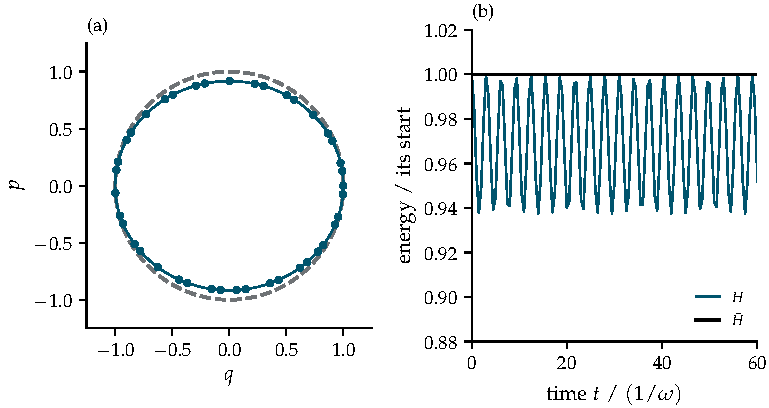
\includegraphics{ch09_integrators/shadow}
\caption{Velocity Verlet for a spring with $m = k = 1$, started at $q = 1$
at rest. (a) Forty steps with $\omega\dt = 0.8$ (dots) lie on the ellipse
of the shadow energy $\tilde{H}$ (solid), slightly lower than the true
curve (dashed). (b) With $\omega\dt = 0.5$, the energy $H$ of the computed
states oscillates in a band, and $\tilde{H}$ stays constant.}
\label{fig:in-shadow}
\end{figure}

The same algebra settles the band that \cref{sec:ha-symplectic} found for
the symplectic Euler method. Its step, $p' = p - \dt\,kq$ and then $q' = q
+ \dt\,p'/m$, keeps exactly
\begin{equation*}
   \frac{p^2}{2m} + \frac12 kq^2 - \frac{\dt\,k}{2m}\,qp
\end{equation*}
(\cref{ex:in-se-shadow}), whose extra term is of first order in $\dt$,
where that of $\tilde{H}$ is of second. Along a curve on which it is
constant, the true energy ranges between $1/(1 + \omega\dt/2)$ and $1/(1 -
\omega\dt/2)$ times it, so for a start at rest, where the two are equal,
between 0.9091 and 1.1111 times its starting value at $\omega\dt = 0.2$:
the band of \cref{fig:ha-maps}. At the same step velocity Verlet keeps a
band of $0.2^2/4 = 1\%$, the narrower band that Chapter~7 promised.

\subsection*{Beyond the spring}

For the spring the shadow energy is found exactly. For a Hamiltonian
whose Taylor series converge, a motion that stays within a bounded
region, and a sufficiently small step, a symplectic method keeps, very nearly and for times that grow
exponentially with $1/\dt$, a shadow energy that differs from $H$ by terms
of the order of its global error, $\dt^2$ for velocity Verlet, and so the
true energy stays within a band of that width without
drifting\cite{LeimkuhlerMatthews2015}. This is the reason, promised in
Chapter~7, why a symplectic step map keeps the energy close. Over long
times no method follows the true motion closely; a symplectic method
follows, exactly for the spring and very nearly in general, the motion of
a slightly different Hamiltonian.

\begin{keyidea}
Velocity Verlet keeps the shadow energy $\tilde{H} = p^2/(2m) + \frac12
kq^2(1 - \omega^2\dt^2/4)$ of a spring exactly, so the true energy
oscillates in a band of relative width $\omega^2\dt^2/4$ without drift,
and the motion runs slightly fast. For smooth Hamiltonians and a
sufficiently small stable step, a nearby shadow energy is kept very
nearly over long times, which explains the small energy fluctuations.
\end{keyidea}

\notebook{09}{the true energy and the shadow energy}

\begin{selfcheck}
At $\omega\dt = 0.2$, what is the relative width of the energy band, and
how fast does the computed motion run?
\end{selfcheck}

%=============================================================================!
% 9.6  STABILITY AND THE SIZE OF THE STEP                                     !
%=============================================================================!
\section{Stability and the size of the step}
\label{sec:in-stability}

Chapters~1, 2 and~4 promised to say how long a step molecular dynamics
can take. Two limits answer it: a step beyond which the computed motion
grows without bound, and, well inside it, the step at which the energy
fluctuates by an acceptable amount. This section derives the first,
measures the second, and turns both into a procedure.

\subsection*{The stability limit}

The shadow energy of \cref{eq:in-shadow} contains the factor $1 -
\omega^2\dt^2/4$. For $\omega\dt < 2$ it is positive, $\tilde{H}$ is a sum
of two positive squares, and its curves are ellipses: the computed motion
stays on one and is bounded. For $\omega\dt > 2$ the factor is negative,
and $\tilde{H} = p^2/(2m) - \frac12 kq^2(\omega^2\dt^2/4 - 1)$ is a
difference of two squares, which stays fixed while $p$ and $q$ both grow
without limit. Its curves are hyperbolas, open curves that run off to
infinity, and the computed motion follows one outwards, its size
multiplied, after the first few steps, by a fixed factor at every step
(\cref{ex:in-growth}). Velocity Verlet is therefore stable for the spring
only when
\begin{equation}
   \omega\,\dt < 2 ,
   \label{eq:in-stable}
\end{equation}
that is, with more than $2\pi/2 = \pi$ steps per period.
\Cref{fig:in-stability} measures it: in 200 steps $\lvert q\rvert$ stays
at 1 up to $\omega\dt = 1.99$, reaches $\num{1.2e17}$ at $2.01$ and
$\num{3e38}$ at $2.05$.

\begin{figure}[htb]
\centering
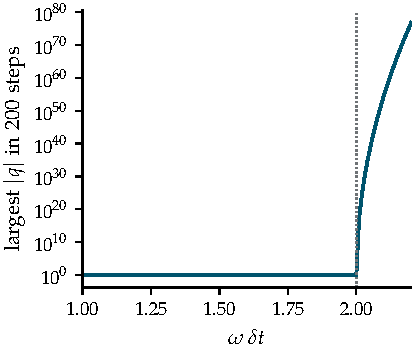
\includegraphics{ch09_integrators/stability}
\caption{The largest $\lvert q\rvert$ reached in 200 steps of velocity
Verlet for a spring started at $q = 1$ at rest, against $\omega\dt$, on a
logarithmic axis; the limit $\omega\dt = 2$ is dotted.}
\label{fig:in-stability}
\end{figure}

Atoms near a minimum of $U$ vibrate in normal modes (\cref{sec:os-modes}).
We write the displacements from the minimum as $\vb{q} = \sum_k
c_k\vb{u}_k$, with $\vb{u}_k$ the patterns of \cref{sec:os-modes}, which
satisfy $\boldsymbol{\Phi}\vb{u}_k = \omega_k^2\vb{M}\vb{u}_k$. When the
forces are linear, pattern $\vb{u}_k$ feels the force
$-\boldsymbol{\Phi}\vb{u}_k = -\omega_k^2\vb{M}\vb{u}_k$, so its
acceleration is $-\omega_k^2\vb{u}_k$: a half kick changes the rate of
change of each $c_k$ by $-\frac12\dt\,\omega_k^2c_k$, a drift changes each
$c_k$ by $\dt$ times its own rate, and velocity Verlet steps every $c_k$ as
it steps a spring of angular frequency $\omega_k$. Each mode must
therefore satisfy \cref{eq:in-stable}: the fastest vibration in the system
sets the limit, however slow everything else is. For the faster O--H
stretch of water, the antisymmetric one, with a period of
\SI{8.88}{\femto\second} (\cref{sec:os-molecules}), $\omega = 2\pi/8.88 =
\SI{0.708}{\radian\per\femto\second}$, and the limit is $\dt < 2/\omega =
\SI{2.83}{\femto\second}$.

\subsection*{Accuracy}

Inside the limit, the energy band of \cref{sec:in-shadow} sets how long a
step is acceptable: for a vibration of angular frequency $\omega$ it
fluctuates by a fraction $\omega^2\dt^2/4$ of the vibration's energy. For
the O--H stretch, a step of \SI{0.5}{\femto\second} gives $\omega\dt =
0.354$ and a band of 3.1\%; \SI{1}{\femto\second} gives 12.5\%. These are
fractions of the energy of the fastest vibration only, but they show why a
step must be short compared with $1/\omega = \SI{1.41}{\femto\second}$, as
\cref{sec:os-molecules} anticipated.

\Cref{fig:in-water} measures this on the spring model of water of
\cref{sec:ro-freedom}, whose fastest vibration, the symmetric stretch,
which the model puts 24\% above the measured value, has $\omega^2 =
\SI{0.7338}{\per\femto\second\squared}$, so $\omega =
\SI{0.857}{\radian\per\femto\second}$ and $2/\omega =
\SI{2.33}{\femto\second}$. Given \SI{0.1}{\electronvolt} of kinetic
energy and followed for \SI{2000}{\femto\second}, its total energy spreads
by \SI{1.3e-3}{\electronvolt}, 1.3\% of the energy put in, with $\dt =
\SI{0.5}{\femto\second}$, and by 9.6\% with \SI{1}{\femto\second}. The
spread grows as $\dt^2$ for the shorter steps (fitted slope 2.02 from 0.05
to \SI{0.5}{\femto\second}) and faster beyond, by a factor of 7.5 from 0.5
to \SI{1}{\femto\second}, where $\omega\dt = 0.86$ is no longer small. The
run blows up at $\dt = \SI{2.3}{\femto\second}$, just inside the limit for
a perfect spring. There $1 - \omega^2\dt^2/4 = 0.030$, so by
\cref{eq:in-shadow} the computed swing of the fastest vibration is
$1/\sqrt{0.030} = 5.8$ times the true one, and over so wide a swing the
springs between atoms are no longer linear in the positions; with
\SI{0.01}{\electronvolt} the same step stays bounded.

\begin{figure}[htb]
\centering
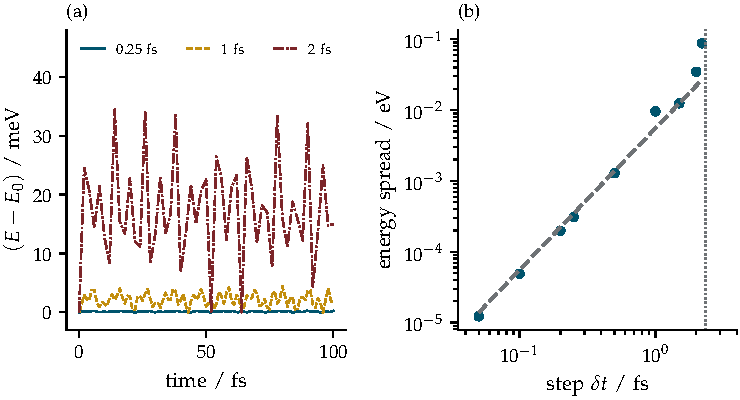
\includegraphics{ch09_integrators/water}
\caption{The spring model of water (\cref{sec:ro-freedom}) followed by
velocity Verlet from its equilibrium geometry with
\SI{0.1}{\electronvolt} of kinetic energy. (a) The total energy relative
to its initial value $E_0 = \SI{0.1}{\electronvolt}$, over the first \SI{100}{\femto\second} for three
steps. (b) The spread of the total energy over \SI{2000}{\femto\second}
against $\dt$, with a line of slope 2 (dashed) and the stability limit
$2/\omega$ of its fastest vibration (dotted); the run at
\SI{2.3}{\femto\second} blew up and is not shown.}
\label{fig:in-water}
\end{figure}

\begin{practice}
The step is chosen by measurement. Without a thermostat, the device of
Chapter~13 that holds the temperature, the total energy should stay
constant, and short runs at two or three steps, such as 0.25, 0.5 and
\SI{1}{\femto\second}, each covering many periods of the vibrations,
record how well it does. Its fluctuation should fall close to $\dt^2$
between the shorter steps, as expected for smooth forces consistent with
the reported energy; it should show no steady
drift; and it should be small compared with the fluctuation of the kinetic
energy, the amount that passes back and forth between kinetic and
potential energy. For the water of \cref{fig:in-water} the ratio of their
standard deviations is 0.9\% at \SI{0.5}{\femto\second} and 6.7\% at
\SI{1}{\femto\second}; how small is acceptable depends on what is to be
measured, and is a judgement. The TrajCast paper gives 0.5 to
\SI{1.0}{\femto\second} as the typical step of molecular dynamics with
forces from electronic structure\cite{Thiemann2026}, and the band of the
O--H stretch above, 3.1\% at \SI{0.5}{\femto\second} and 12.5\% at
\SI{1}{\femto\second}, shows why bonds to hydrogen hold it there. Without
hydrogen the fastest vibrations are slower, and longer steps pass the same
test (for the lithium model alone, \cref{ex:in-lithium}; in graphite the
vibrations of the carbon atoms must pass it too). At half the limit,
$\omega\dt = 1$, the band of the fastest vibration is already 25\%.
Chapter~11 removes the fastest vibrations by holding bonds at fixed
length.
\end{practice}

The stability limit has a cousin in \cref{sec:mo-atoms}: saving the
positions of an oscillation needs enough frames per period to recover its
velocity, and computing the motion needs more than $\pi$ steps per period
to remain bounded at all.

\begin{keyidea}
Velocity Verlet is stable only for $\omega\dt < 2$ for every vibration, so
the fastest one sets the limit, \SI{2.83}{\femto\second} for the O--H
stretch. Accuracy demands a much shorter step: the energy of a vibration
fluctuates by $\omega^2\dt^2/4$, and the step is chosen by measuring the
energy fluctuation of short runs.
\end{keyidea}

\notebook{09}{push the step to the stability limit}

\begin{selfcheck}
The model lithium atom rattling in its hollow (\cref{sec:os-small}) has a
period of \SI{170.3}{\femto\second}. What is the stability limit for the
step?
\end{selfcheck}

%=============================================================================!
% 9.7  LONG RUNS AND ROUGH FORCES                                             !
%=============================================================================!
\section{Long runs and rough forces}
\label{sec:in-long}

A method of higher order makes a smaller error over a fixed time. A
simulation, however, runs for very many periods of its fastest motion,
and over such times what matters is whether the energy, and with it the
statistics of Chapter~12, stays right. This section compares velocity Verlet with a method of fourth
order over a long run, and measures what a force that jumps costs, as
\cref{sec:pe-cutoffs} promised.

\subsection*{A fourth-order method}

The classical Runge--Kutta method of fourth order, RK4, advances the pair
$\vb{w} = (x, v)$, whose rate of change is $\vb{g}(\vb{w}) = (v, a(x))$,
by four samples of that rate, each taken at a point reached with the one
before:
\begin{align*}
   \vb{s}_1 &= \vb{g}(\vb{w}_n) , &
   \vb{s}_2 &= \vb{g}\bigl(\vb{w}_n + \tfrac12\dt\,\vb{s}_1\bigr) ,\\
   \vb{s}_3 &= \vb{g}\bigl(\vb{w}_n + \tfrac12\dt\,\vb{s}_2\bigr) , &
   \vb{s}_4 &= \vb{g}(\vb{w}_n + \dt\,\vb{s}_3) ,
\end{align*}
\begin{equation*}
   \vb{w}_{n+1} = \vb{w}_n + \tfrac16\dt\,(\vb{s}_1 + 2\vb{s}_2
   + 2\vb{s}_3 + \vb{s}_4) .
\end{equation*}
Its derivation, matching this to the Taylor series up to $\dt^4$, is
long, and we take it on trust. In \cref{fig:in-orders} its error after a
time of 4 is $\num{1.6e-9}$ at $\dt = 0.05$, against $\num{4.1e-5}$ for
velocity Verlet, and falls roughly as $\dt^4$: the error changes sign
between $\dt = 0.1$ and 0.05, so the points scatter about the line of
slope 4, with a fitted slope of 4.3. It calls for the forces four times
per step, and it is neither symplectic nor reversible: for the spring a
step multiplies areas by $c^2 + s^2 < 1$ (\cref{ex:in-rk4-spring}), and
reversing the velocity and stepping again returns the start only to
within that factor.

\Cref{fig:in-long}(a) follows the 32-atom Lennard-Jones cluster of
\cref{sec:pe-cutoffs} for $200\tau$, where $\tau = \sigma\sqrt{m/
\varepsilon}$ is the unit of time of \cref{eq:pe-tau}, with velocity Verlet at $\dt =
0.005\tau$ and RK4 at $\dt = 0.02\tau$, so that each calls for the forces
40\,000 times. The energy of velocity Verlet stays within a band of
$\num{3.4e-3}\,\varepsilon$; that of RK4 falls steadily, by
$0.64\varepsilon$ in all, as if a drag acted on the atoms. For a spring,
\cref{ex:in-rk4-spring} shows that every step of RK4 multiplies the energy
by a number slightly less than 1. Over a long run the symplectic method
keeps the energy better: it keeps a shadow energy (\cref{sec:in-shadow}),
while RK4 shrinks areas and keeps no such energy.

\subsection*{Forces that jump}

\Cref{fig:in-long}(b) repeats the velocity Verlet run with the potential
cut off at $2.5\sigma$, once shifted, so that the force jumps when a pair
crosses the cutoff, and once switched smoothly between $2\sigma$ and
$2.5\sigma$. With switching the energy stays in a band of
$\num{3.4e-3}\,\varepsilon$, as without a cutoff. With shifting the
centre of the band wanders: the mean energy over the second half of the
run is $\num{1.4e-3}\,\varepsilon$ below that over the first, against
$\num{4e-6}\,\varepsilon$ with switching, and the range over the run grows
to $\num{6.3e-3}\,\varepsilon$. Each jump of the force inside a step breaks
the Taylor series on which the method's accuracy rests, and leaves an
error that the next steps do not undo. A force that is not smooth lets
the energy of a fixed-step method wander, which is why the smooth cutoffs of \cref{sec:pe-cutoffs},
and the smooth envelopes of machine-learned potentials, matter.

\begin{figure}[htb]
\centering
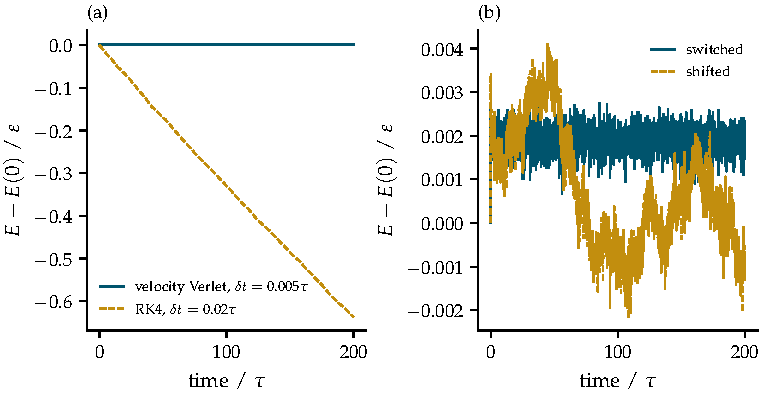
\includegraphics{ch09_integrators/long}
\caption{The 32-atom Lennard-Jones cluster of \cref{sec:pe-cutoffs} over
$200\tau$, as the change of its total energy. (a) Velocity Verlet with
$\dt = 0.005\tau$ and RK4 with $\dt = 0.02\tau$, which call for the forces
equally often. (b) Velocity Verlet with $\dt = 0.005\tau$ and the
potential cut at $2.5\sigma$ by switching and by shifting.}
\label{fig:in-long}
\end{figure}

\begin{keyidea}
Over a long run a symplectic method of second order keeps the energy in a
band, while RK4, more accurate over a short time and four times as
costly per step, lets it drift. Forces that jump inside a step let the
energy wander out of its band, so the forces of a simulation must be
smooth.
\end{keyidea}

\notebook{09}{long runs with velocity Verlet and RK4}

\begin{selfcheck}
To cover \SI{1}{\pico\second}, how many force evaluations does velocity
Verlet need with $\dt = \SI{0.5}{\femto\second}$, and how many does RK4 need
with $\dt = \SI{2}{\femto\second}$?
\end{selfcheck}

%=============================================================================!
% 9.S  WHAT WE NOW HAVE                                                       !
%=============================================================================!
\unnumbered{What we now have}

A method of computing motion is a step map, and its order says how fast
its error over a fixed time shrinks with the step: the forward Euler
method, whose error over a fixed time shrinks as $\dt$ and over one step
as $\dt^2$, is of order 1. Adding the Taylor
series a step ahead and a step behind gives the Verlet method, which in
its velocity form is a half kick, a drift and a half kick, costs one force
evaluation per step and is of order 2; its local error, of order
$\dt^3$, is the `cubic scaling' quoted by TrajCast.

Reversing the
velocities after a step and stepping again returns the start, with its
velocities reversed, without error, and each step keeps
volume in phase space and satisfies the full symplectic condition. The
same method follows from splitting the Liouville operator into the parts
that move positions and momenta, whose exponentials are a drift and a kick
with no error; the symmetric product agrees with the true motion to second
order.

For a spring, velocity Verlet keeps the shadow energy $p^2/(2m) +
\frac12 kq^2(1 - \omega^2\dt^2/4)$ exactly, so the true energy oscillates
in a band of relative width $\omega^2\dt^2/4$; the symplectic Euler
method keeps one that differs from the energy at first order in $\dt$,
hence its wider band, and for other Hamiltonians a nearby shadow energy
is kept very nearly for sufficiently small steps and smooth forces.

The method is stable only for
$\omega\dt < 2$ for the fastest vibration, \SI{2.83}{\femto\second} for
the O--H stretch, and accurate enough well inside that; the step is chosen
by measuring the energy fluctuation. Over long runs it keeps the energy
better than RK4 at the same cost, provided the forces are smooth.

Chapter~10 uses velocity Verlet to build a complete simulation: atoms in a
periodic box, neighbour lists for the cutoffs, and the Ewald sum for
charges.

%=============================================================================!
% 9.A  ANSWERS TO THE CHECKS                                                  !
%=============================================================================!
\unnumbered{Answers to the checks}
\label{sec:in-answers}

\answerto{sec:in-steps}Dividing by $4 = 2^2$ means the global error is of
order $\dt^2$, so the method is of order 2, and its local error is of
order $\dt^3$.

\answerto{sec:in-verlet}With $a_n = a_{n+1} = -g$, \cref{eq:in-vv} gives
$x_{n+1} = x_n + \dt\,v_n - \frac12 g\dt^2$ and $v_{n+1} = v_n - g\dt$, the
exact motion of \cref{sec:mo-integrating} over a time $\dt$, so no error
is made at any step.

\answerto{sec:in-reversal}$\partial x'/\partial x = 1$, $\partial x'/
\partial v = 0$, $\partial v'/\partial x = \frac12\dt\,\dd a/\dd x$ and
$\partial v'/\partial v = 1$, so the determinant is $1\times1 -
0\times\frac12\dt\,\dd a/\dd x = 1$.

\answerto{sec:in-splitting}With $\Liou = (p/m)\,\partial/\partial q$,
$\Liou q^2 = 2qp/m$, $\Liou^2q^2 = 2p^2/m^2$ and $\Liou^3q^2 = 0$, so
$\mathrm{e}^{\dt\Liou}q^2 = q^2 + 2qp\,\dt/m + p^2\dt^2/m^2 = (q +
\dt\,p/m)^2$.

\answerto{sec:in-shadow}$\omega^2\dt^2/4 = 0.04/4 = 0.01$, a band of 1\%;
$\cos\tilde\omega\dt = 1 - 0.02 = 0.98$ gives $\tilde\omega\dt = 0.2003$,
so the motion runs 0.17\% fast.

\answerto{sec:in-stability}$\omega = 2\pi/170.3 =
\SI{0.0369}{\radian\per\femto\second}$, so $\dt < 2/\omega =
\SI{54.2}{\femto\second}$.

\answerto{sec:in-long}Velocity Verlet: $1000/0.5 = 2000$ steps of one
force evaluation each, 2000. RK4: $1000/2 = 500$ steps of four, also 2000.

%=============================================================================!
% 9.E  EXERCISES                                                              !
%=============================================================================!
\unnumbered{Exercises}
\label{sec:in-exercises}

The exercises run from questions of understanding, through calculations,
to short derivations marked `show that'. Full solutions are in
\hyperref[sec:in-solutions]{`Solutions to the exercises'} at the end of
the book, and Notebook~09 checks every numerical answer.

\begin{exercise}[Euler and a falling ball]
\label{ex:in-fall}
Show that forward Euler steps of $\dt$ for a body falling from $x_0$ with
velocity $v_0$ under the acceleration $-g$ give, after $n$ steps,
$x_n = x_0 + v_0n\dt - \frac12 g\dt^2n(n - 1)$, and that at the time
$t_{\mathrm f} = n\dt$ the error is $\frac12 gt_{\mathrm f}\dt$, of order
$\dt$.
\end{exercise}

\begin{exercise}[reading an order]
\label{ex:in-read}
Halving the step divides a method's error at a given time by 16. What is
its order, and its local error?
\end{exercise}

\begin{exercise}[the error of Störmer--Verlet]
\label{ex:in-stormer}
Show that the term of order $\dt^4$ in $x(t + \dt) + x(t - \dt)$ is
$\frac1{12}\ddot{a}\,\dt^4$, so that the local error of
\cref{eq:in-stormer} is $\frac1{12}\ddot{a}\,\dt^4$.
\end{exercise}

\begin{exercise}[velocities from positions]
\label{ex:in-central}
With $x_{n\pm1}$ the true positions $x(t \pm \dt)$, show that $(x_{n+1} -
x_{n-1})/(2\dt)$ differs from the true velocity $v(t)$ by
$\frac16\dot{a}\,\dt^2$ plus terms of higher order.
\end{exercise}

\begin{exercise}[the local error of velocity Verlet]
\label{ex:in-local}
Show that the position after one step of \cref{eq:in-vv} from a correct
start differs from the true one by $\frac16\dot{a}\,\dt^3$ plus terms of
higher order.
\end{exercise}

\begin{exercise}[leapfrog]
\label{ex:in-leapfrog}
Show that the positions of the leapfrog method, $v_{n+\frac12} =
v_{n-\frac12} + \dt\,a_n$ and $x_{n+1} = x_n + \dt\,v_{n+\frac12}$, obey
\cref{eq:in-stormer}.
\end{exercise}

\begin{exercise}[Euler does not run backwards]
\label{ex:in-euler-reverse}
For a spring with $m = k = 1$, take one forward Euler step from $(q, v) =
(1, 0)$, reverse the velocity and take another. Where does it land?
\end{exercise}

\begin{exercise}[one coordinate]
\label{ex:in-omega}
Show that for a $2\times2$ matrix $\vb{J}$, $\vb{J}^{\mathsf T}
\boldsymbol{\Omega}\vb{J} = (\det\vb{J})\,\boldsymbol{\Omega}$, with
$\boldsymbol{\Omega} = \bigl(\begin{smallmatrix}0 & 1\\ -1 &
0\end{smallmatrix}\bigr)$, so that for one coordinate the symplectic
condition is $\det\vb{J} = 1$.
\end{exercise}

\begin{exercise}[the unsymmetric product]
\label{ex:in-unsymmetric}
Show that $\mathrm{e}^{\dt X}\mathrm{e}^{\dt Y}$ and $\mathrm{e}^{\dt(X +
Y)}$ differ at second order by $\frac12\dt^2(XY - YX)$.
\end{exercise}

\begin{exercise}[which acts first]
\label{ex:in-order}
For one coordinate, show that $\mathrm{e}^{\dt\Liou_{\mathrm p}}\mathrm{e}^{
\dt\Liou_{\mathrm r}}$ applied to $q$ gives $q + \dt\,\bigl(p + \dt\,
F(q)\bigr)/m$: a kick, then a drift.
\end{exercise}

\begin{exercise}[a drift of a function]
\label{ex:in-drift}
With $\Liou_{\mathrm r} = (p/m)\,\partial/\partial q$, show from the
series that $\mathrm{e}^{\dt\Liou_{\mathrm r}}q^3 = (q + \dt\,p/m)^3$.
\end{exercise}

\begin{exercise}[the shadow energy]
\label{ex:in-shadow}
Complete the derivation of \cref{sec:in-shadow}: put $p_{\frac12} = p' +
\frac12\dt\,kq'$ into $p_{\frac12}^2/(2m) + \frac12 kq'^2 - \bigl(\dt\,
k/(2m)\bigr)\,q'p_{\frac12}$ and show that the result is $\tilde{H}(q',
p')$.
\end{exercise}

\begin{exercise}[the band of symplectic Euler]
\label{ex:in-se-shadow}
Show that the symplectic Euler step for the spring, $p' = p - \dt\,kq$
and then $q' = q + \dt\,p'/m$, keeps $p^2/(2m) + \frac12 kq^2 - \bigl(\dt
\,k/(2m)\bigr)\,qp$. Writing $q = A\cos\phi$ and $p/(m\omega) =
A\sin\phi$, as for the circle of \cref{sec:os-circle}, show that along a curve on which this is constant the
energy $H$ ranges between $1/(1 + \omega\dt/2)$ and $1/(1 - \omega\dt/2)$
times it.
\end{exercise}

\begin{exercise}[the step's matrix]
\label{ex:in-trace}
Show that one step of velocity Verlet for the spring is $q' = (1 -
\frac12\omega^2\dt^2)\,q + (\dt/m)\,p$ and $p' = -k\dt\,(1 - \frac14
\omega^2\dt^2)\,q + (1 - \frac12\omega^2\dt^2)\,p$, and that its matrix,
the Jacobian matrix of the step, has determinant 1 and trace, the sum of
its diagonal entries, $2 - \omega^2\dt^2$.
\end{exercise}

\begin{exercise}[growth beyond the limit]
\label{ex:in-growth}
Beyond the limit the computed motion grows by a factor $\lvert\lambda
\rvert$ per step, with $\lambda$ the eigenvalue of larger size of the
step's matrix, a root of $\lambda^2 - (2 - \omega^2\dt^2)\lambda + 1 = 0$,
the characteristic equation with the trace and determinant of
\cref{ex:in-trace} (the toolbox of \cref{sec:in-reversal}). Find the
factor at $\omega\dt = 2.05$.
\end{exercise}

\begin{exercise}[a step for water]
\label{ex:in-water}
What is the longest step for which the energy of the antisymmetric O--H
stretch, of period \SI{8.88}{\femto\second}, fluctuates by no more than 3\%?
\end{exercise}

\begin{exercise}[a step for lithium]
\label{ex:in-lithium}
For the model lithium atom in its hollow, of period
\SI{170.3}{\femto\second}, find the step that keeps its energy band to
1\%, and compare it with the stability limit.
\end{exercise}

\begin{exercise}[steps per period]
\label{ex:in-per-period}
What is $2\pi/(\omega\dt)$, the number of steps per period, for which
velocity Verlet keeps an energy band of 1\%?
\end{exercise}

\begin{exercise}[RK4 and a spring]
\label{ex:in-rk4-spring}
For the spring, one RK4 step in the variables $q$ and $u = v/\omega$ is
$q' = cq + su$ and $u' = -sq + cu$, with $c = 1 - \frac12x^2 +
\frac1{24}x^4$, $s = x - \frac16x^3$ and $x = \omega\dt$. Show that it
multiplies $q^2 + u^2$, and so the energy, by $c^2 + s^2 = 1 -
\frac1{72}x^6 + \frac1{576}x^8$, and find the fraction of the energy lost
in 10\,000 steps at $x = 0.2$.
\end{exercise}

\begin{exercise}[a learned long step]
\label{ex:in-long-step}
A learned propagator predicts the state of water \SI{5}{\femto\second}
ahead, ten steps of \SI{0.5}{\femto\second}. What is $\omega\dt$ for the
O--H stretch at a step of \SI{5}{\femto\second}, and could velocity
Verlet take it?
\end{exercise}

\begin{exercise}[a shifted line]
\label{ex:in-spectrum}
A simulation of water with $\dt = \SI{0.7}{\femto\second}$ runs the O--H
stretch slightly fast. At what wavenumber does the antisymmetric stretch,
\SI{3756}{\per\centi\metre} (period \SI{8.88}{\femto\second}), appear in
it?
\end{exercise}


%=============================================================================!
% CHAPTER 10  BUILDING A MOLECULAR DYNAMICS CODE                              !
%=============================================================================!
\chapter{Building a molecular dynamics code}
\label{ch:code}

%=============================================================================!
% 10.0  CHAPTER OPENING                                                       !
%=============================================================================!
The earlier chapters followed a handful of atoms in empty space. To
represent a liquid or a crystal, we need a sample packed at the material's
density whose atoms have neighbours on every side. Repeating a simulation
cell supplies those neighbours, but also changes how we find separations
and sum the forces. We develop these operations first, including the
Ewald sum for charges, then use neighbour lists to avoid testing every
pair at every step.

With the forces defined, we can prepare the positions and velocities and
advance them with the velocity Verlet loop of Chapter~9. Comparisons with
an independent library check the implementation, and timings identify
where compiled code can reduce its cost. Chapter~11 starts from this loop
and asks how far the step can be lengthened by constraining stiff bonds
and evaluating slowly changing forces less often.

%=============================================================================!
% 10.1  A BOX REPEATED IN EVERY DIRECTION                                     !
%=============================================================================!
\section{A box repeated in every direction}
\label{sec:md-periodic}

A sample small enough to simulate is mostly surface. This section counts
how much, removes the surface by repeating a box of atoms in every
direction, and sets up the coordinates that describe such a box.

\subsection*{Most of a small sample is surface}

We place $N = n^3$ atoms on a cubic grid, $n$ along each edge. The atoms that
are not on a face form a smaller cube of $(n - 2)^3$, so the fraction on
the surface is
\begin{align*}
   1 - \frac{(n - 2)^3}{n^3} &= 1 - \Bigl(1 - \frac2n\Bigr)^3\\
   &= \frac6n - \frac{12}{n^2} + \frac8{n^3}
   && \text{expanding $(1 - x)^3 = 1 - 3x + 3x^2 - x^3$ with $x = 2/n$,}
\end{align*}
close to $6/n$ when $n$ is large. A thousand atoms ($n = 10$) have 49\%
of them on the surface, about ten thousand ($n = 22$) 25\%, and a million ($n =
100$) still 5.9\%. A surface atom has fewer neighbours than one inside,
and a sample this small would measure the properties of its surface as
much as those of its bulk.

\subsection*{The periodic box}

The surface is removed by repeating the box. The atoms sit in a cell,
and the cell and its contents are copied without end in every direction,
so that space is filled with identical cells. An atom that leaves through
one face of the cell comes in through the opposite face, as its copy from
the neighbouring cell enters, and every atom has neighbours on all sides;
a ship in an old arcade game that leaves the screen at the right edge and
reappears at the left lives in such a box, in two dimensions. Each atom
feels the others and their copies. The price is an imposed periodicity:
the sample repeats with the period of the cell, no wave longer than the
cell, such as a long sound wave, can occur, and for a short-ranged
potential the cell must be large enough that an atom does not feel its
own copies (\cref{sec:md-image}); the Coulomb energy of
\cref{sec:md-ewald} includes them by design.

The cell is a parallelepiped, a box whose six faces are parallelograms,
spanned by three lattice vectors $\vb{a}$,
$\vb{b}$ and $\vb{c}$, which we place as the columns of the cell matrix
\begin{equation}
   \vb{h} = \begin{pmatrix} \vb{a} & \vb{b} & \vb{c} \end{pmatrix} .
   \label{eq:md-cell}
\end{equation}
For a cubic cell of side $L$, $\vb{a} = (L, 0, 0)$, $\vb{b} = (0, L, 0)$,
$\vb{c} = (0, 0, L)$ and $\vb{h}$ is $L$ times the identity. Any position
can be written as $\vb{r} = s_1\vb{a} + s_2\vb{b} + s_3\vb{c}$, which is
$\vb{h}$ times the vector $\vb{s} = (s_1, s_2, s_3)$: row $x$ of $\vb{h}$
is $(a_x, b_x, c_x)$, so the $x$ component of $\vb{h}\vb{s}$ is $a_xs_1 +
b_xs_2 + c_xs_3$, the $x$ component of $s_1\vb{a} + s_2\vb{b} +
s_3\vb{c}$, and likewise for $y$ and $z$. So
\begin{equation}
   \vb{r} = \vb{h}\vb{s} , \qquad \vb{s} = \vb{h}^{-1}\vb{r} ,
   \label{eq:md-fractional}
\end{equation}
with the inverse matrix of \cref{sec:ro-remove}. The inverse exists: a
matrix without one turns some $\vb{s} \neq \vb{0}$ into $\vb{0}$, and
$s_1\vb{a} + s_2\vb{b} + s_3\vb{c} = \vb{0}$ would put the three lattice
vectors in one plane, a flat cell with no volume. The numbers $s_1$, $s_2$
and $s_3$ are the fractional coordinates of the position: the point lies
inside the cell when each is between 0 and 1, and its copies are at
$\vb{h}(\vb{s} + \vb{n})$, with $\vb{n}$ any vector of three whole
numbers, positive, negative or zero.

The volume of the cell is its base times its height. The face spanned by
$\vb{b}$ and $\vb{c}$ is a parallelogram of area $\lvert\vb{b}\times\vb{c}
\rvert$ (\cref{sec:ro-cross}), and $\vb{b}\times\vb{c}$ is at right
angles to that face. The height of the cell above it is the size of the
part of $\vb{a}$ along that direction, the scalar product of $\vb{a}$
with the vector of length one $(\vb{b}\times\vb{c})/\lvert\vb{b}\times
\vb{c}\rvert$ (\cref{sec:mo-plane}), taken without its sign, since
$\vb{a}$ may lie on either side of the face. Then
\begin{align}
   V &= \lvert\vb{b}\times\vb{c}\rvert\,
        \frac{\lvert\vb{a}\cdot(\vb{b}\times\vb{c})\rvert}
             {\lvert\vb{b}\times\vb{c}\rvert}
     && \text{base times height}\notag\\
     &= \lvert\vb{a}\cdot(\vb{b}\times\vb{c})\rvert ,
     && \text{cancelling $\lvert\vb{b}\times\vb{c}\rvert$}
   \label{eq:md-volume}
\end{align}
the scalar triple product of \cref{sec:ro-tensor}. For the cubic cell, $V =
L^3$.

\subsection*{Wrapping and unwrapping}

To put a position back into the cell, we take its fractional coordinates
and subtract from each its floor,
\begin{equation*}
   \vb{s} \to \vb{s} - \lfloor\vb{s}\rfloor ,
\end{equation*}
where the floor $\lfloor x\rfloor$ of a number $x$ is the largest whole
number not above it, and $\lfloor\vb{s}\rfloor$ takes the floor of each
coordinate: $\lfloor 2.3\rfloor = 2$ and $\lfloor -0.4\rfloor = -1$, so
2.3 becomes 0.3 and $-0.4$ becomes 0.6.
This is wrapping. The function \texttt{wrap} of \texttt{mdlab.cell} does
it for $N$ atoms:

\begin{code}
def wrap(positions: ArrayLike, cell: ArrayLike) -> NDArray:
    s = to_fractional(positions, cell)
    return to_cartesian(s - np.floor(s), cell)
\end{code}

\noindent where \texttt{to\_fractional} solves $\vb{h}\vb{s} = \vb{r}$
for each atom and \texttt{to\_cartesian} multiplies back.

The integration itself does not need wrapped positions: the forces depend
only on separations, and \cref{sec:md-image} reduces each separation to
its nearest copy whichever copy of each atom the code holds. \texttt{mdlab} therefore follows
each atom's path without wrapping, so that its displacement over a run can
be read off directly, and wraps the positions only when it writes them to
a file, as files of periodic systems usually hold them. To recover a
continuous path from wrapped frames, each frame's position is replaced by
its copy nearest to the previous frame's, which is right as long as no
atom moves more than half the narrowest width of the cell between frames
(\cref{sec:md-image}): a longer move is mistaken for a shorter one the
other way, as too few frames per period hid an oscillation in
\cref{sec:mo-atoms}.

\subsection*{Momentum in a periodic box}

Moving every atom by the same displacement moves each of its copies with
it and changes no separation, so the forces still add to zero and the
total momentum is conserved, as \cref{sec:ha-noether} found, whether a
pair interacts through its nearest copy (\cref{sec:md-image}) or through
all of them (\cref{sec:md-ewald}). Turning the atoms is not
a symmetry of the box, and the angular momentum is not conserved. In the
run of 500 atoms of \cref{sec:md-loop} the largest component of the total
momentum after 2000 steps is $\num{3.8e-15}$\,amu\,\AA/fs, the rounding of
the arithmetic.

\begin{keyidea}
A cell repeated in every direction removes the surface that would
dominate any sample small enough to simulate. The cell is described by
the matrix $\vb{h}$ of its lattice vectors; positions have fractional
coordinates $\vb{s} = \vb{h}^{-1}\vb{r}$, the cell has volume $\lvert
\vb{a}\cdot(\vb{b}\times\vb{c})\rvert$, and wrapping subtracts from
each fractional coordinate its floor.
\end{keyidea}

\notebook{10}{wrap atoms into a cubic and a hexagonal cell}

\begin{selfcheck}
In the cell with $\vb{a} = (4, 0, 0)$, $\vb{b} = (0, 5, 0)$ and $\vb{c} =
(0, 0, 6)$\,\AA, what are the fractional coordinates of $\vb{r} = (9,
-1, 3)$\,\AA, and where does wrapping put it?
\end{selfcheck}

%=============================================================================!
% 10.2  THE NEAREST IMAGE                                                     !
%=============================================================================!
\section{The nearest image}
\label{sec:md-image}

Two atoms in a periodic box are separated by $\vb{r}_{ij} = \vb{r}_j -
\vb{r}_i$, written $\vb{d}$ in this section to keep subscripts short, and
by every copy of it, $\vb{d} + \vb{h}\vb{n}$. A copy is also called an
image, and the nearest copy the minimum image. A pair
potential cut off at $r_{\mathrm c}$ needs the copies within $r_{\mathrm c}$,
and when the cell is large enough there is at most one, the nearest. This
section finds it, first in a rectangular cell and then in a skewed one,
and derives how large the cell must be.

\subsection*{Rounding the fractional coordinates}

The fractional coordinates of the separation, $\vb{s} = \vb{h}^{-1}\vb{d}$,
and those of a copy, $\vb{h}^{-1}(\vb{d} + \vb{h}\vb{n}) = \vb{s} +
\vb{n}$, differ by whole numbers. Rounding
each to the nearest whole number and subtracting,
\begin{equation}
   \vb{s} \to \vb{s} - \operatorname{round}(\vb{s}) ,
   \label{eq:md-round}
\end{equation}
gives the copy whose fractional coordinates all lie between $-\frac12$
and $\frac12$. The function \texttt{minimum\_image} of \texttt{mdlab.cell}
does this for many separations at once:

\begin{code}
def minimum_image(separations: ArrayLike, cell: ArrayLike) -> NDArray:
    s = to_fractional(separations, cell)
    return to_cartesian(s - np.round(s), cell)
\end{code}

In a rectangular cell, with $\vb{a}$, $\vb{b}$ and $\vb{c}$ along the
axes and of lengths $a$, $b$ and $c$, a copy is $\vb{d} + (n_1a, n_2b,
n_3c)$ and its squared length is
\begin{equation*}
   (d_x + n_1a)^2 + (d_y + n_2b)^2 + (d_z + n_3c)^2 .
\end{equation*}
Each term depends on one whole number only, so each is made as small as it
can be on its own, by the $n_1$ that brings $d_x + n_1a$ between
$-\frac12a$ and $\frac12a$, and likewise for the others. That is
\cref{eq:md-round}: in a rectangular cell, rounding gives the nearest copy
of every separation.

\subsection*{A skewed cell}

Many crystals have cells that are not rectangular. Graphite's is
hexagonal: in each layer $\vb{a}$ and $\vb{b}$ have the same length, $a =
\SI{2.464}{\angstrom}$, at \ang{120} to each other, and $\vb{c}$, of length
\SI{6.711}{\angstrom}, is at right angles to the layers\cite{TrucanoChen1975}.
Rounding in such a cell returns the copy inside the parallelogram of
\cref{fig:md-cell}(a), centred on the first atom, while the copies that
are nearest fill the hexagon around it: a separation is its own nearest
copy when it ends nearer to the first atom than to any copy of that atom,
and in the plane of a layer the six closest copies, at $\pm\vb{a}$,
$\pm\vb{b}$ and $\pm(\vb{a} + \vb{b})$, cut off a hexagon whose sides
halve the lines to them. The two regions overlap but
differ: in about 17\% of the parallelogram, shaded, a shorter copy
exists, and rounding misses it.

\begin{figure}[htb]
\centering
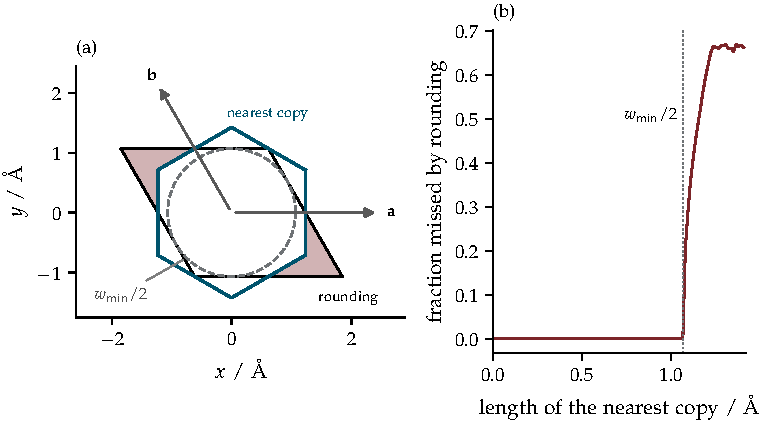
\includegraphics{ch10_code/cell}
\caption{Rounding and the nearest copy in the hexagonal cell of graphite,
in the plane of a layer. (a) Rounding returns separations in the
parallelogram centred on the first atom, spanned by $\vb{a}$ and
$\vb{b}$; the separations that are their own nearest copy fill the
hexagon; in the shaded corners a shorter copy exists. The circle of radius
$\frac12w_{\min}$, half the smallest perpendicular width, lies inside both.
(b) Of the separations that are their own nearest copy, the fraction that
rounding returns wrongly, against their length: none below
$\frac12w_{\min}$ (dotted).}
\label{fig:md-cell}
\end{figure}

Rounding cannot fail for a short enough separation, whatever the cell.
Since $\vb{b}$ and $\vb{c}$ are at right angles to $\vb{b}\times\vb{c}$,
taking the scalar product of $\vb{d} = s_1\vb{a} + s_2\vb{b} + s_3\vb{c}$
with $\vb{b}\times\vb{c}$ leaves only the first term,
\begin{equation*}
   \vb{d}\cdot(\vb{b}\times\vb{c}) = s_1\,\vb{a}\cdot(\vb{b}\times\vb{c}) .
\end{equation*}
Dividing by $\vb{a}\cdot(\vb{b}\times\vb{c})$, whose size is $V$ by
\cref{eq:md-volume},
\begin{align}
   \lvert s_1\rvert
   &= \frac{\lvert\vb{d}\cdot(\vb{b}\times\vb{c})\rvert}{V}
   && \text{dividing and taking sizes}\notag\\
   &\le \frac{\lvert\vb{d}\rvert\,\lvert\vb{b}\times\vb{c}\rvert}{V}
   && \text{a scalar product is at most the product of the lengths}
   \notag\\
   &= \frac{\lvert\vb{d}\rvert}{w_1} ,
   \qquad w_1 = \frac{V}{\lvert\vb{b}\times\vb{c}\rvert}
   && \text{naming the width.}
   \label{eq:md-width}
\end{align}
The length $w_1$ is the height of the cell above the face spanned by
$\vb{b}$ and $\vb{c}$ (\cref{sec:md-periodic}), the perpendicular width
of the cell in that direction; $w_2$ and $w_3$ follow in the same way.
Two consequences follow, with $w_{\min}$ the smallest of the three widths.
\begin{itemize}
\item A copy shorter than $\frac12w_{\min}$ has every fractional
   coordinate between $-\frac12$ and $\frac12$, so rounding returns it:
   rounding finds the nearest copy of every separation shorter than half
   the smallest width, in any cell. \Cref{fig:md-cell}(b) measures this
   for graphite: rounding first misses just beyond $\frac12w_{\min} =
   \SI{1.067}{\angstrom}$.
\item A copy $\vb{h}\vb{n}$ of the origin, with $\vb{n}$ not zero, has a
   fractional coordinate of size at least 1, so by \cref{eq:md-width} it is
   at least $w_{\min}$ long. Two copies of one separation differ by such
   a vector, and a difference of two vectors is no longer than the sum of
   their lengths (one side of a triangle is no longer than the other two
   together), so they cannot both be shorter than $\frac12w_{\min}$.
\end{itemize}
A cutoff no larger than half the smallest width therefore makes rounding
exact for every pair within it, in any cell, and each pair has at most one
copy within it:
\begin{equation}
   r_{\mathrm c} \le \tfrac12 w_{\min} .
   \label{eq:md-rule}
\end{equation}
For a rectangular cell the widths are the side lengths. For graphite they
are \SI{2.134}{\angstrom} in the layers and \SI{6.711}{\angstrom} across
them, so a single cell allows a cutoff of only \SI{1.067}{\angstrom}.
Repeating the cell $n_1$ times along $\vb{a}$, $n_2$ times along $\vb{b}$
and $n_3$ times along $\vb{c}$ makes a larger cell, a supercell, of volume
$n_1n_2n_3V$, whose face $n_2\vb{b}\times n_3\vb{c}$ has area
$n_2n_3\lvert\vb{b}\times\vb{c}\rvert$, so its first width is $n_1w_1$,
and likewise $n_2w_2$ and $n_3w_3$. A cutoff of \SI{10}{\angstrom} then
needs $n_1, n_2 \ge 20/2.134 = 9.4$ and $n_3 \ge 20/6.711 = 2.98$: a
supercell of $10\times10\times3$ of these cells, 1200 atoms at the four
atoms per cell of \cref{sec:md-start}.

\begin{practice}
\Cref{eq:md-rule} decides the smallest cell that rounding can serve. A
skewed cell is narrower than its lattice vectors are long: graphite's
in-plane vectors are \SI{2.464}{\angstrom} long, and its cell is
\SI{2.134}{\angstrom} wide. When a cell must be narrower than twice the
cutoff, as for a single cell of a crystal, the copies within the cutoff
are found by searching over several neighbouring cells instead, as the
Ewald sum of \cref{sec:md-ewald} does. \texttt{nearest\_image} of
\texttt{mdlab.cell} searches in the same way but keeps only the shortest
copy, the reference against which rounding is tested.
\end{practice}

\begin{keyidea}
Rounding the fractional coordinates of a separation gives the copy inside
the cell centred on the first atom. In a rectangular cell that is always
the nearest copy; in any cell it is the nearest for every separation
shorter than half the smallest perpendicular width $w_{\min}$, the
smallest of $V/\lvert\vb{b}\times\vb{c}\rvert$ and its two partners, so
a cutoff $r_{\mathrm c} \le \frac12w_{\min}$ makes the minimum image
exact.
\end{keyidea}

\notebook{10}{compare rounding with the nearest copy in a hexagonal cell}

\begin{selfcheck}
A cubic cell of side \SI{20}{\angstrom} holds atoms that interact with a
cutoff of \SI{12}{\angstrom}. Is rounding enough to find their pairs, and
how large must the cell be?
\end{selfcheck}

%=============================================================================!
% 10.3  CHARGES IN A PERIODIC BOX: THE EWALD SUM                              !
%=============================================================================!
\section{Charges in a periodic box: the Ewald sum}
\label{sec:md-ewald}

The electrostatic energy of charges $q_i$ in a periodic box is
\begin{equation}
   U = \frac12\sum_{i,j}\sideset{}{'}\sum_{\vb{n}}
   \frac{k_{\mathrm e}q_iq_j}{\lvert\vb{r}_j - \vb{r}_i + \vb{h}\vb{n}\rvert} ,
   \label{eq:md-coulomb}
\end{equation}
summed over every pair and every copy, the prime leaving out an atom with
itself, $i = j$ at $\vb{n} = \vb{0}$. \Cref{sec:pe-coulomb} found that sums
of this kind converge so slowly that their value depends on the order of
the terms. Ewald's method\cite{Ewald1921} splits each $1/r$ into a part
that dies away quickly, summed over the near copies, and a smooth part,
summed as a series of waves. This section derives it with two new tools.

\subsection*{Two tools}

\begin{toolbox}[Gaussian integrals]
A Gaussian is the bell-shaped curve $\mathrm{e}^{-ax^2}$, with $a > 0$.
An integral to infinity is the limit of the integral to $X$ as $X$ grows.
For $I = \int_{-\infty}^{\infty}\mathrm{e}^{-x^2}\dd x$, the square $I^2$
is the limit of $\int_{-X}^{X}\mathrm{e}^{-x^2}\dd x\int_{-X}^{X}
\mathrm{e}^{-y^2}\dd y$. Written as sums of values times short steps, the
product of the two is a sum over small rectangles of $\mathrm{e}^{-x^2}
\mathrm{e}^{-y^2} = \mathrm{e}^{-(x^2 + y^2)}$ times their areas $\dd x\,
\dd y$, so $I^2$ is the integral of $\mathrm{e}^{-(x^2 + y^2)}$ over the
whole plane (\cref{sec:en-curl}); the square of side $2X$ lies between the
discs of radius $X$ and $\sqrt2\,X$, and the integrand is positive, so
discs give the same limit. Likewise an integral over a volume, written
$\int\dots\dd^3r$, is the limit of a sum of values times the volumes
$\dd^3r$ of small boxes, and over all space the integral of a product
$f_1(x)f_2(y)f_3(z)$ is the product of three ordinary integrals. The
integrand $\mathrm{e}^{-(x^2 + y^2)}$ depends only on the distance $r =
\sqrt{x^2 + y^2}$ from the origin, so we cut the plane into rings of
radius $r$ and width $\dd r$, of area $2\pi r\,\dd r$:
\begin{equation*}
   I^2 = \int_0^{\infty}\mathrm{e}^{-r^2}\,2\pi r\,\dd r
   = \Bigl[-\pi\mathrm{e}^{-r^2}\Bigr]_0^{\infty} = \pi ,
   \qquad I = \sqrt\pi .
\end{equation*}
\emph{Changing the variable.} If $u = g(x)$ and $F' = f$, the chain rule
(\cref{sec:mo-acceleration}) gives $\frac{\dd}{\dd x}F(g(x)) =
f(g(x))\,g'(x)$, so by the fundamental theorem of calculus
(\cref{sec:mo-integrating}) both $\int_{x_1}^{x_2}f(g(x))\,g'(x)\,\dd x$
and $\int_{g(x_1)}^{g(x_2)}f(u)\,\dd u$ equal $F(g(x_2)) - F(g(x_1))$: an
integral in $u$ becomes one in $x$ on writing $\dd u = g'(x)\,\dd x$ and
moving the limits to match. With $u = \sqrt a\,x$, for $a > 0$,
\begin{equation*}
   \int_{-\infty}^{\infty}\mathrm{e}^{-ax^2}\dd x
   = \frac1{\sqrt a}\int_{-\infty}^{\infty}\mathrm{e}^{-u^2}\dd u
   = \sqrt{\frac{\pi}{a}} .
\end{equation*}
\emph{The error function} is $\operatorname{erf}(x) = (2/\sqrt\pi)
\int_0^x\mathrm{e}^{-u^2}\dd u$, which rises from 0 at $x = 0$ to 1 as $x$
grows, since $\mathrm{e}^{-u^2}$ takes the same value at $u$ and $-u$, so
that its integral from 0 to infinity is half of $I$, $\frac12\sqrt\pi$;
its complement is $\operatorname{erfc}(x) = 1 - \operatorname{erf}(x) =
(2/\sqrt\pi)\int_x^{\infty}\mathrm{e}^{-u^2}\dd u$. For small $x$ the
integrand is close to 1, so $\operatorname{erf}(x) \approx 2x/\sqrt\pi$.
For large $x$, since $u^2 \ge x^2 + 2x(u - x)$, $\int_x^{\infty}
\mathrm{e}^{-u^2}\dd u \le \mathrm{e}^{-x^2}\int_x^{\infty}\mathrm{e}^{-2x(u
- x)}\dd u = \mathrm{e}^{-x^2}/(2x)$, so $\operatorname{erfc}(x) \le
\mathrm{e}^{-x^2}/(\sqrt\pi\,x)$: it falls roughly as $\mathrm{e}^{-x^2}$.
\end{toolbox}

\begin{toolbox}[Fourier series on a periodic cell]
A smooth function $f(x)$ that repeats with period $L$ can be written as a
sum of waves that repeat with it, $\cos(2\pi mx/L)$ and $\sin(2\pi mx/L)$
for $m = 0, 1, 2, \dots$, each with its own coefficient; we take this on
trust. The coefficients are found by averaging. Adding the two cosine
formulae of \cref{eq:mo-addition} gives $\cos A\cos B = \frac12[\cos(A -
B) + \cos(A + B)]$, and adding the two sine formulae gives $\sin A\cos B =
\frac12[\sin(A + B) + \sin(A - B)]$. A cosine or a sine averages to zero
over whole periods, so the average over one period of $\cos(2\pi mx/L)
\cos(2\pi m'x/L)$ is $\frac12$ if $m = m' \neq 0$ and zero if $m \neq m'$,
and that of $\sin(2\pi mx/L)\cos(2\pi m'x/L)$ is zero: multiplying the
series by one cosine and averaging leaves half that wave's coefficient
(the whole of it for $m = 0$).

In three dimensions the waves are $\cos(\vb{G}\cdot\vb{r})$ and
$\sin(\vb{G}\cdot\vb{r})$, and they repeat with the cell when
$\vb{G}\cdot\vb{h}\vb{n}$ is a multiple of $2\pi$ for every $\vb{n}$. This
holds for $\vb{G} = m_1\vb{a}^* + m_2\vb{b}^* + m_3\vb{c}^*$, with whole
numbers $m_1$, $m_2$ and $m_3$ and reciprocal vectors $\vb{a}^*$,
$\vb{b}^*$ and $\vb{c}^*$ chosen so that $\vb{a}\cdot\vb{a}^* =
\vb{b}\cdot\vb{b}^* = \vb{c}\cdot\vb{c}^* = 2\pi$ and every other such
product, such as $\vb{a}\cdot\vb{b}^*$, is zero, since then
$\vb{G}\cdot\vb{h}\vb{n} = \vb{G}\cdot(n_1\vb{a} + n_2\vb{b} + n_3\vb{c})
= 2\pi(m_1n_1 + m_2n_2 + m_3n_3)$. Since $\vb{h}^{-1}\vb{h}$ is the
identity, row $j$ of $\vb{h}^{-1}$ times column $i$ of $\vb{h}$ is 1 for
$i = j$ and 0 otherwise, so the reciprocal vectors are $2\pi$ times the
rows of $\vb{h}^{-1}$; and as $s_j$ is row $j$ of $\vb{h}^{-1}$ times
$\vb{r}$, $\vb{G}\cdot\vb{r} = 2\pi(m_1s_1 + m_2s_2 + m_3s_3) =
2\pi\,\vb{m}\cdot\vb{s}$, with $\vb{m} = (m_1, m_2, m_3)$. For a cubic
cell of side $L$ the reciprocal vectors have length $2\pi/L$ along the
axes. The vectors $\vb{G}$ are said to lie in reciprocal space.

The average of a wave over the cell is zero unless $\vb{G} = \vb{0}$. In
fractional coordinates the cell is the unit cube, whose image under $\vb{r}
= \vb{h}\vb{s}$ has volume $V$, so each small box of volume $\dd^3s$
becomes one of volume $V\,\dd^3s$ and the average is $\int\cos(2\pi\,
\vb{m}\cdot\vb{s})\,\dd^3s$ over the unit cube. Taking $m_1 \neq 0$
(otherwise any other $m_j$ that is not zero serves), the integral over
$s_1$ alone, with $s_2$ and $s_3$ held fixed, is $[\sin(2\pi\vb{m}\cdot
\vb{s})/(2\pi m_1)]$ between $s_1 = 0$ and 1, which is zero because the
sine repeats. For a function with $f(-\vb{r}) = f(\vb{r})$ only cosines
are needed, since $f(\vb{r}) = \frac12[f(\vb{r}) + f(-\vb{r})]$ and every
sine cancels between the two series; summing over all $\vb{G}$ with
$c_{-\vb{G}} = c_{\vb{G}}$,
\begin{equation*}
   f(\vb{r}) = \sum_{\vb{G}}c_{\vb{G}}\cos(\vb{G}\cdot\vb{r}) ,
   \qquad
   c_{\vb{G}} = \frac1V\int_{\text{cell}}f(\vb{r})\cos(\vb{G}\cdot\vb{r})
   \,\dd^3r ,
\end{equation*}
because the cell average of $\cos(\vb{G}\cdot\vb{r})\cos(\vb{G}'\cdot
\vb{r})$, by the product formula, is $\frac12$ for $\vb{G}' = \vb{G}$,
$\frac12$ for $\vb{G}' = -\vb{G}$, and zero otherwise (both halves at once
when $\vb{G} = \vb{0}$), so that the cell average of $f(\vb{r})\cos(\vb{G}
\cdot\vb{r})$ is $\frac12c_{\vb{G}} + \frac12c_{-\vb{G}} = c_{\vb{G}}$.
\end{toolbox}

The cosine integral of a Gaussian follows from these. Let $F(G) =
\int_{-\infty}^{\infty}\mathrm{e}^{-ax^2}\cos(Gx)\,\dd x$ for a number $G$,
so that $F(0) = \sqrt{\pi/a}$. The integral is a limit of sums, and the
derivative of a sum is the sum of the derivatives, so $F'(G)$ is the
integral of the derivative of $\mathrm{e}^{-ax^2}\cos(Gx)$ with respect to
$G$, $-x\,\mathrm{e}^{-ax^2}\sin(Gx)$ by the chain rule. Integrating by
parts (\cref{sec:la-euler}) with $\sin(Gx)$ and $x\mathrm{e}^{-ax^2} =
\frac{\dd}{\dd x}\bigl(-\mathrm{e}^{-ax^2}/(2a)\bigr)$, whose product
vanishes at both ends,
\begin{equation*}
   F'(G) = -\int x\,\mathrm{e}^{-ax^2}\sin(Gx)\,\dd x
   = -\frac{G}{2a}\int\mathrm{e}^{-ax^2}\cos(Gx)\,\dd x
   = -\frac{G}{2a}\,F(G) .
\end{equation*}
By the product rule (\cref{sec:ne-drag}) and the chain rule,
\begin{equation*}
   \frac{\dd}{\dd G}\Bigl[\mathrm{e}^{G^2/(4a)}F(G)\Bigr]
   = \mathrm{e}^{G^2/(4a)}\Bigl[\frac{G}{2a}F(G) + F'(G)\Bigr] = 0 ,
\end{equation*}
so $\mathrm{e}^{G^2/(4a)}F(G)$ keeps its value $F(0)$ at $G = 0$:
\begin{equation}
   \int_{-\infty}^{\infty}\mathrm{e}^{-ax^2}\cos(Gx)\,\dd x
   = \sqrt{\frac{\pi}{a}}\;\mathrm{e}^{-G^2/(4a)} .
   \label{eq:md-gauss-cos}
\end{equation}
A narrow Gaussian, large $a$, has a wide spread of waves, and a wide one a
narrow spread.

\subsection*{Splitting the Coulomb energy}

With $u = rt$, the first Gaussian integral gives
\begin{equation*}
   \frac{2}{\sqrt\pi}\int_0^{\infty}\mathrm{e}^{-r^2t^2}\dd t
   = \frac{2}{\sqrt\pi}\,\frac1r\int_0^{\infty}\mathrm{e}^{-u^2}\dd u
   = \frac1r ,
\end{equation*}
and splitting the range of $t$ at a chosen $\alpha$ splits $1/r$ in two,
\begin{equation}
   \frac1r = \frac{\operatorname{erfc}(\alpha r)}{r}
   + \frac{\operatorname{erf}(\alpha r)}{r} ,
   \label{eq:md-split}
\end{equation}
the first from $t > \alpha$ and the second from $t < \alpha$, by the same
change of variable. By the bound in the toolbox, the first part falls
roughly as $\mathrm{e}^{-\alpha^2r^2}$, so its sum over the copies
converges quickly and in any order:
\begin{equation*}
   U_{\mathrm{real}} = \frac12\sum_{i,j}\sideset{}{'}\sum_{\vb{n}}k_{\mathrm e}
   q_iq_j\,\frac{\operatorname{erfc}(\alpha r_{ij\vb{n}})}{r_{ij\vb{n}}} ,
   \qquad r_{ij\vb{n}} = \lvert\vb{r}_j - \vb{r}_i + \vb{h}\vb{n}\rvert ,
\end{equation*}
taken over the copies closer than a cutoff at which $\operatorname{erfc}$
has fallen to nothing that matters. The second part of \cref{eq:md-split}
tends to the finite value $2\alpha/\sqrt\pi$ as $r \to 0$, by the
small-$x$ form of $\operatorname{erf}$, and falls only as $1/r$: it
carries the long range, and it is smooth.

\subsection*{The smooth part as waves}

Summed over the copies, the second part is, by its integral over $t$,
\begin{equation*}
   \Phi_{\mathrm s}(\vb{d}) = \sum_{\vb{n}}\frac{\operatorname{erf}(\alpha
   \lvert\vb{d} + \vb{h}\vb{n}\rvert)}{\lvert\vb{d} + \vb{h}\vb{n}\rvert}
   = \frac{2}{\sqrt\pi}\int_0^{\alpha}g_t(\vb{d})\,\dd t ,
   \qquad g_t(\vb{d}) = \sum_{\vb{n}}\mathrm{e}^{-\lvert\vb{d} + \vb{h}\vb{n}
   \rvert^2t^2} .
\end{equation*}
Neither side is finite as it stands, since the terms fall only as
$1/\lvert\vb{d} + \vb{h}\vb{n}\rvert$ (\cref{sec:pe-coulomb}); the trouble
sits in a single wave, found below. The function $g_t$, a Gaussian placed
at every copy of the origin, repeats with the cell and is unchanged by
$\vb{d} \to -\vb{d}$. Its Fourier coefficients are
\begin{equation*}
   c_{\vb{G}} = \frac1V\int_{\text{cell}}\sum_{\vb{n}}\mathrm{e}^{-\lvert
   \vb{r} + \vb{h}\vb{n}\rvert^2t^2}\cos(\vb{G}\cdot\vb{r})\,\dd^3r
   = \frac1V\int_{\text{all space}}\mathrm{e}^{-\lvert\vb{r}\rvert^2t^2}
   \cos(\vb{G}\cdot\vb{r})\,\dd^3r ,
\end{equation*}
because, writing $\vb{r}' = \vb{r} + \vb{h}\vb{n}$, the term of copy
$\vb{n}$ is the integral of $\mathrm{e}^{-\lvert\vb{r}'\rvert^2t^2}
\cos(\vb{G}\cdot\vb{r}')$ over the cell shifted by $\vb{h}\vb{n}$, as
$\cos(\vb{G}\cdot\vb{r}' - \vb{G}\cdot\vb{h}\vb{n}) =
\cos(\vb{G}\cdot\vb{r}')$, and the shifted cells, one for every $\vb{n}$,
fill space once. The Gaussian depends only on $\lvert\vb{r}\rvert$, so
turning the axes changes nothing, and with the $x$ axis along $\vb{G}$ the
integral is a product of three, one by \cref{eq:md-gauss-cos} with $a =
t^2$ and $G = \lvert\vb{G}\rvert$, and two plain Gaussian integrals:
\begin{equation*}
   c_{\vb{G}} = \frac1V\,\frac{\sqrt\pi}{t}\,\mathrm{e}^{-G^2/(4t^2)}
   \times\frac{\sqrt\pi}{t}\times\frac{\sqrt\pi}{t}
   = \frac{\pi^{3/2}}{Vt^3}\,\mathrm{e}^{-G^2/(4t^2)} .
\end{equation*}
Integrating over $t$ from 0 to $\alpha$, with $u = G^2/(4t^2)$, so that
$\dd u = -G^2\,\dd t/(2t^3)$ and the limits $t = 0$ and $\alpha$ become $u
= \infty$ and $G^2/(4\alpha^2)$, whose exchange cancels the minus sign,
gives for $\vb{G} \neq \vb{0}$
\begin{equation*}
   \frac{2}{\sqrt\pi}\,\frac{\pi^{3/2}}{V}\int_0^{\alpha}\frac{\mathrm{e}^{
   -G^2/(4t^2)}}{t^3}\,\dd t
   = \frac{2\pi}{V}\,\frac{2}{G^2}\int_{G^2/(4\alpha^2)}^{\infty}
   \mathrm{e}^{-u}\,\dd u
   = \frac{4\pi}{VG^2}\,\mathrm{e}^{-G^2/(4\alpha^2)} ,
\end{equation*}
so that
\begin{equation*}
   \Phi_{\mathrm s}(\vb{d}) = \frac{4\pi}{V}\sum_{\vb{G}\neq\vb{0}}
   \frac{\mathrm{e}^{-G^2/(4\alpha^2)}}{G^2}\cos(\vb{G}\cdot\vb{d})
   + (\text{the }\vb{G} = \vb{0}\text{ term}) .
\end{equation*}
The terms die away as $\mathrm{e}^{-G^2/(4\alpha^2)}$: a smooth function
needs only a few waves. For $\vb{G} = \vb{0}$ the coefficient is
$\pi^{3/2}/(Vt^3)$, whose integral over $t$ grows without limit as $t \to
0$. Starting the integral at a small $t_0$ in place of 0 gives
$(2/\sqrt\pi)\int_{t_0}^{\alpha}\pi^{3/2}/(Vt^3)\,\dd t = \pi/(Vt_0^2) -
\pi/(V\alpha^2)$, a constant that does not depend on $\vb{d}$; in the
energy it is multiplied by $\sum_{i,j}q_iq_j = (\sum_iq_i)^2$, which for a
neutral cell is zero whatever $t_0$, and the term is dropped. What is
dropped is the part of the sum that depended on its order: dropping it
gives the energy of the periodic sample surrounded by a conductor, a
material in which charge moves freely, and other surroundings add a term
in the cell's dipole moment $\sum_iq_i\vb{r}_i$, which measures how far
its positive and negative charges sit apart\cite{deLeeuw1980}.

\subsection*{The energy}

The smooth parts of all pairs give $\frac12k_{\mathrm e}\sum_{i,j}q_iq_j
\,\Phi_{\mathrm s}(\vb{r}_j - \vb{r}_i)$, with every pair taken twice and
each atom with itself. By the addition formula, $\cos(\vb{G}\cdot\vb{r}_j
- \vb{G}\cdot\vb{r}_i) = \cos(\vb{G}\cdot\vb{r}_j)\cos(\vb{G}\cdot
\vb{r}_i) + \sin(\vb{G}\cdot\vb{r}_j)\sin(\vb{G}\cdot\vb{r}_i)$, and the
double sum separates into squares of single sums,
\begin{align*}
   \sum_{i,j}q_iq_j\cos(\vb{G}\cdot\vb{r}_j - \vb{G}\cdot\vb{r}_i)
   &= \mathcal{C}(\vb{G})^2 + \mathcal{S}(\vb{G})^2 ,\\
   \mathcal{C}(\vb{G}) = \sum_iq_i\cos(\vb{G}\cdot\vb{r}_i) ,
   &\qquad \mathcal{S}(\vb{G}) = \sum_iq_i\sin(\vb{G}\cdot\vb{r}_i) ,
\end{align*}
the structure factor, which costs $N$ operations for each $\vb{G}$. The
smooth part of each atom with itself at $\vb{n} = \vb{0}$ is not in
\cref{eq:md-coulomb} and must be taken out: it is $\frac12k_{\mathrm e}
q_i^2$ times the limit $2\alpha/\sqrt\pi$. Altogether,
\begin{equation}
   U = U_{\mathrm{real}}
   + \frac{2\pi k_{\mathrm e}}{V}\sum_{\vb{G}\neq\vb{0}}
   \frac{\mathrm{e}^{-G^2/(4\alpha^2)}}{G^2}\bigl(\mathcal{C}(\vb{G})^2
   + \mathcal{S}(\vb{G})^2\bigr)
   - k_{\mathrm e}\frac{\alpha}{\sqrt\pi}\sum_iq_i^2 ,
   \label{eq:md-ewald}
\end{equation}
the real-space sum, over copies; the reciprocal-space sum, over the
waves; and the self term. The forces are the slopes of each part of
\cref{eq:md-ewald} (\cref{ex:md-forces}). The function
\texttt{ewald\_energy\_forces} of \texttt{mdlab.ewald} computes them; its
reciprocal sum is

\begin{code}
    weight = np.exp(-g2 / (4 * alpha**2)) / g2
    phase = r @ g.T
    cos, sin = np.cos(phase), np.sin(phase)
    c_sum, s_sum = q @ cos, q @ sin
    e_rec = 2 * np.pi / volume * np.sum(weight * (c_sum**2 + s_sum**2))
\end{code}

\noindent with \texttt{g} the vectors $\vb{G}$ kept, one per row,
\texttt{g2} their squared lengths, and $k_{\mathrm e}$ left out: the
function multiplies every part by it at the end. It also wraps the
positions into the cell first, since its search over copies in real space
starts from there.

A cell that is not neutral, with total charge $Q = \sum_iq_i$, has no
finite energy in a periodic box: the $\vb{G} = \vb{0}$ term,
$\frac12k_{\mathrm e}Q^2[\pi/(Vt_0^2) - \pi/(V\alpha^2)]$, grows without
limit as $t_0 \to 0$. It is made neutral by a uniform background of charge
$-Q$ spread over the cell. The background has only the $\vb{G} = \vb{0}$
wave and meets the charges and itself through the whole of $1/r$, the
integral over $t$ from $t_0$ to infinity, $\pi/(Vt_0^2)$; its energy with
the charges, $-k_{\mathrm e}Q^2\pi/(Vt_0^2)$, and with itself,
$\frac12k_{\mathrm e}Q^2\pi/(Vt_0^2)$, cancel the growing part and leave
$-\pi k_{\mathrm e}Q^2/(2V\alpha^2)$. With it, the energy of five charges
adding to 1.7 in a cubic cell of side \SI{6}{\angstrom} is
$\SI{-11.1048563570}{\electronvolt}$ at $\alpha = 0.5$, 0.8 and
\SI{1.2}{\per\angstrom}, to \SI{3e-10}{\electronvolt}; without it, it moves
by \SI{1.0}{\electronvolt} over the same range.

\subsection*{Choosing \texorpdfstring{$\alpha$}{alpha} and the cutoffs}

The total does not depend on $\alpha$, which only moves work between the
two sums. \Cref{fig:md-ewald}(a) shows this for rock salt in its cubic
cell of side $2d$: as $\alpha$ goes from $0.6/d$ to $5/d$ the real-space
part changes by about 1, the reciprocal-space part by about 4 and the
self part by about 5, in units of $k_{\mathrm e}/d$, and their sum stays
at $-1.7475646\,k_{\mathrm e}/d$ per ion pair, $-\mathcal{M}k_{\mathrm
e}/d$ with Chapter~8's Madelung constant\cite{Evjen1932}, to
$\num{2e-12}\,k_{\mathrm e}/d$. Each sum is cut where its terms have
fallen to about a chosen size $\epsilon_{\mathrm E}$, the real-space terms
falling roughly as $\mathrm{e}^{-\alpha^2r^2}$: $\mathrm{e}^{-\alpha^2
r_{\mathrm c}^2} = \epsilon_{\mathrm E}$ in real space and
$\mathrm{e}^{-G_{\mathrm c}^2/(4\alpha^2)} = \epsilon_{\mathrm E}$ in
reciprocal space, so
\begin{equation*}
   r_{\mathrm c} = \frac{\sqrt{-\ln\epsilon_{\mathrm E}}}{\alpha} ,
   \qquad
   G_{\mathrm c} = 2\alpha\sqrt{-\ln\epsilon_{\mathrm E}} ,
\end{equation*}
and the error of the energy follows $\epsilon_{\mathrm E}$
(\cref{fig:md-ewald}b), in steps because the copies and the waves come in
shells. Careful estimates of these errors are due to Kolafa and
Perram\cite{KolafaPerram1992}.

\begin{figure}[htb]
\centering
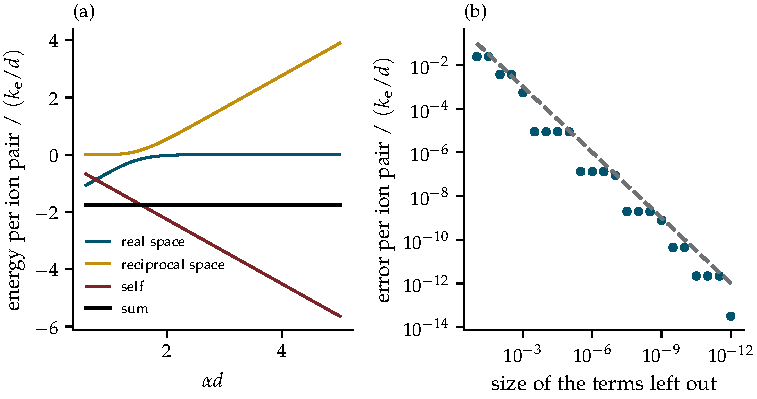
\includegraphics{ch10_code/ewald}
\caption{The Ewald sum of rock salt in its cubic cell of side $2d$, with
$k_{\mathrm e} = 1$. (a) The real-space, reciprocal-space and self parts
of the energy per ion pair against $\alpha$, and their sum, $-1.7475646$
at every $\alpha$. (b) The error of the sum against the size of the terms
left out, at $\alpha = 2/d$, with a line of slope 1 (dashed).}
\label{fig:md-ewald}
\end{figure}

Three further checks pass. The same Madelung constant comes from a
supercell of $2\times2\times2$ cubic cells and from the skewed cell of two
ions spanned by $(0, 1, 1)d$, $(1, 0, 1)d$ and $(1, 1, 0)d$, 1.747564595
in each to ten figures; in a skewed cell of six charges the forces agree
with central differences of the energy (\cref{sec:pe-forces}) to
$\num{7.4e-10}$\,eV/\AA, against forces of up to
\SI{15}{\electronvolt\per\angstrom}, and add to zero to
$\num{1.2e-14}$\,eV/\AA.

The cost of the method grows faster than $N$: at a fixed density, with
$\alpha$ chosen to balance the two sums, it grows as $N^{3/2}$
(\cref{ex:md-cost}), provided the real-space sum finds its pairs through a
cell list (\cref{sec:md-neighbours}). \texttt{mdlab} chooses $\alpha$ this
way by default but tests every pair against every nearby copy, so its own
cost grows as $N^2$, which is fine for the small cells of this chapter. Particle mesh Ewald methods spread the
charges onto a grid and sum the waves with the fast Fourier transform of
Chapter~16, at a cost that grows as $N\ln N$\cite{Darden1993,Essmann1995},
and are what large simulations of charged systems use.

\Needspace{12\baselineskip}
\begin{bridge}
Many electronic-structure calculations in periodic cells, those that
expand in plane waves among them, find the electrostatic (Hartree)
potential of the electron density with the same Fourier series, one
coefficient $4\pi\rho_{\vb{G}}/G^2$ per wave of the density $\rho$ in
atomic units, find the energy of the nuclei with one another by an Ewald
sum, and leave out the $\vb{G} = \vb{0}$ terms, which for a charged cell
amounts to the uniform neutralising background. The background brings in
spurious energies of the charge with its copies and with the background,
which fall only as $1/L$ with the size of the cell and need
corrections\cite{MakovPayne1995}. A slab with a different charge or
adsorbate on each face carries a dipole, and because the potential must
take the same value at both ends of a periodic cell, the step in potential
across the dipole is undone by an artificial field across the vacuum,
which a dipole correction removes\cite{NeugebauerScheffler1992,Bengtsson1999}:
the situation of a charged electrode in a periodic cell.
\end{bridge}

\begin{keyidea}
Ewald's method splits $1/r$ into $\operatorname{erfc}(\alpha r)/r$, summed
over near copies, and $\operatorname{erf}(\alpha r)/r$, smooth, whose sum
over copies is a Fourier series with coefficients $4\pi\mathrm{e}^{-G^2/
(4\alpha^2)}/(VG^2)$. With the self term removed and the $\vb{G} =
\vb{0}$ term dropped for a neutral cell, the energy does not depend on
$\alpha$, and it reproduces the Madelung constant of rock salt.
\end{keyidea}

\notebook{10}{move the work between the two Ewald sums with \texorpdfstring{$\alpha$}{alpha}}

\begin{selfcheck}
For $\epsilon_{\mathrm E} = 10^{-8}$ and $\alpha = \SI{0.3}{\per\angstrom}$,
what are the real-space cutoff and $G_{\mathrm c}$?
\end{selfcheck}

%=============================================================================!
% 10.4  NEIGHBOUR LISTS                                                       !
%=============================================================================!
\section{Neighbour lists}
\label{sec:md-neighbours}

A pair potential cut off at $r_{\mathrm c}$ needs only the pairs closer than
$r_{\mathrm c}$, and in a dense system each atom has a few dozen of them
whatever the size of the system. Testing every pair to find them costs
work that grows as $N^2$, which \cref{sec:pe-cutoffs} promised to reduce
to $N$. This section does so with two lists.

\subsection*{How many pairs matter}

In a liquid of number density $\rho$ (atoms per unit volume), the
neighbours of an atom within $r_{\mathrm c}$ fill a sphere of volume
$\frac43\pi r_{\mathrm c}^3$, so there are about $\frac43\pi r_{\mathrm
c}^3\rho$ of them, and half as many pairs per atom, since each pair has
two atoms. For a dense Lennard-Jones liquid, $\rho = 0.8\sigma^{-3}$, and
$r_{\mathrm c} = 2.5\sigma$, that is 52.4 neighbours and 26 pairs per
atom, against $N(N - 1)/2$ pairs to test. Measured on atoms placed at
random at this density, every $N$ from 500 to 32\,000 gives 26.0 to 26.4
pairs per atom.

\subsection*{The cell list}

The cell is divided into small cells at least $r_{\mathrm c}$ wide: along
the direction of each perpendicular width $w_k$ of \cref{sec:md-image},
there are $n_k = \lfloor w_k/r_{\mathrm c}\rfloor$ of them, each a slice
$1/n_k$ thick in the fractional coordinate $s_k$. Each atom is sorted, in
one pass over the atoms, into the small cell numbered $\lfloor
n_ks_k\rfloor$ along each direction, with $\vb{s}$ wrapped into the cell.
A partner within $r_{\mathrm c}$ changes $s_k$ by less than $r_{\mathrm
c}/w_k \le 1/n_k$ (\cref{eq:md-width}), less than one slice, so it lies
in the atom's own small cell or in one of the $3^3 - 1 = 26$ that touch
it, and only those are searched. A small cell holds on average the same number of
atoms whatever $N$, so the work per atom does not grow with $N$ and the
total grows as $N$. With fewer than three small cells along some
direction, the 26 neighbours would include one cell twice, and
\texttt{mdlab} tests all pairs instead. The method goes back to Quentrec
and Brot\cite{QuentrecBrot1973}.

\Cref{fig:md-neighbours} measures both: testing all pairs grows with a
slope of 2.02 on logarithmic axes, the cell list, from $N = 2000$ on,
with a slope of 0.98. The two cost the same near $N = 1000$, and at $N =
4000$ the cell list is four times faster. At $N = 32\,000$ the cell list
takes \SI{0.78}{\second}; testing all pairs, which takes
\SI{0.42}{\second} at $N = 4000$, would by its slope of 2 take $8^2 = 64$
times as long there, about \SI{27}{\second}.

\begin{figure}[htb]
\centering
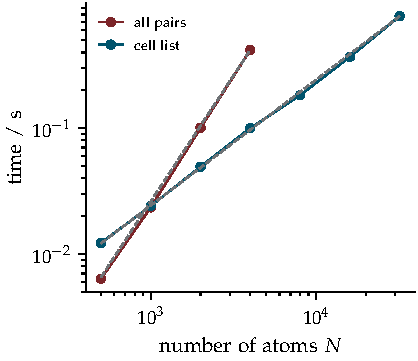
\includegraphics{ch10_code/neighbours}
\caption{The time to find every pair within $r_{\mathrm c} = 2.5\sigma$ of
$N$ atoms placed at random at $\rho = 0.8\sigma^{-3}$, by testing all
pairs and through a cell list, against $N$, with lines of slope 2 and 1
(dashed).}
\label{fig:md-neighbours}
\end{figure}

\subsection*{The Verlet list}

Atoms move little in a step, so the pairs within $r_{\mathrm c}$ change
little from one step to the next. Verlet's list\cite{Verlet1967} keeps the
pairs within $r_{\mathrm c} + r_{\mathrm{skin}}$, where the skin
$r_{\mathrm{skin}}$ is a margin added to the cutoff, and reuses them for
many steps, computing at each step only the distances of the listed pairs.
It must be rebuilt before a pair missing from it can come within
$r_{\mathrm c}$. Suppose that since the list was built every atom has
moved less than $\frac12r_{\mathrm{skin}}$, atom $i$ by
$\Delta\vb{r}_i$. A pair not on the list was then at least $r_{\mathrm c}
+ r_{\mathrm{skin}}$ apart. The straight line from $i$'s old position to
$j$'s old position is no longer than the detour through $i$'s new position
and $j$'s new position, since two sides of a triangle are together at
least as long as the third, used once for each triangle of the detour:
\begin{align*}
   r_{ij}^{\text{then}} &\le \lvert\Delta\vb{r}_i\rvert + r_{ij}^{\text{now}}
   + \lvert\Delta\vb{r}_j\rvert ,\\
   r_{ij}^{\text{now}} &\ge r_{ij}^{\text{then}} - \lvert\Delta\vb{r}_i\rvert
   - \lvert\Delta\vb{r}_j\rvert > (r_{\mathrm c} + r_{\mathrm{skin}})
   - \tfrac12r_{\mathrm{skin}} - \tfrac12r_{\mathrm{skin}} = r_{\mathrm c}
   && \text{rearranging.}
\end{align*}
The list is therefore complete until some atom has moved half the skin,
and is rebuilt then. The class \texttt{VerletList} of
\texttt{mdlab.neighbours} keeps the positions at the last build and tests
this at every step:

\begin{code}
    def needs_rebuild(self, positions: ArrayLike) -> bool:
        if self.reference is None:
            return True
        if not np.array_equal(self.cell, self.built_cell):
            return self._strained_needs_rebuild(positions)
        moved = minimum_image(
            np.asarray(positions, dtype=float) - self.reference, self.cell
        )
        return bool(
            np.max(np.einsum("ix,ix->i", moved, moved))
            > (0.5 * self.skin) ** 2
        )
\end{code}

\noindent The second test applies only when the cell itself has changed
since the list was built, as it does under the barostats of
Chapter~14 (\cref{sec:pr-npt}); with the cell fixed the method goes on to
the rule just derived. The displacements are reduced to their nearest
copy so that the
test stays right if the positions have been wrapped back into the cell,
when an atom that crossed a face would otherwise seem to have moved a
whole cell; \texttt{einsum} adds the squares of the three components of
each displacement, and comparing squared lengths with
$(\frac12r_{\mathrm{skin}})^2$ avoids a square root per atom. The list
holds pairs out to $r_{\mathrm c} + r_{\mathrm{skin}}$, so
\cref{eq:md-rule} applies to that distance, $r_{\mathrm c} +
r_{\mathrm{skin}} \le \frac12w_{\min}$, and \texttt{mdlab} refuses a
smaller cell. A thicker skin means fewer rebuilds and more pairs to check
at each step. In the argon run of \cref{sec:md-loop}, with a skin of
\SI{1}{\angstrom}, the list is built 187 times in 2000 steps, about every
eleventh step, each time by testing all pairs: its box of
\SI{26.3}{\angstrom} holds only $\lfloor26.3/9.5\rfloor = 2$ small cells
of $r_{\mathrm c} + r_{\mathrm{skin}} = \SI{9.5}{\angstrom}$ along each
side.

\begin{keyidea}
Each atom has about $\frac43\pi r_{\mathrm c}^3\rho$ neighbours within the
cutoff. A cell list finds them by searching only neighbouring small cells,
at a cost that grows as $N$; a Verlet list with a skin
$r_{\mathrm{skin}}$ reuses the pairs within $r_{\mathrm c} +
r_{\mathrm{skin}}$ until some atom has moved $\frac12r_{\mathrm{skin}}$.
\end{keyidea}

\notebook{10}{time all pairs against the cell list}

\begin{selfcheck}
With $r_{\mathrm c} = 2.5\sigma$ and a skin of $0.3\sigma$, how far may
the atoms move before the Verlet list must be rebuilt, and about how many
pairs per atom does the list hold at $\rho = 0.8\sigma^{-3}$?
\end{selfcheck}

%=============================================================================!
% 10.5  STARTING A SIMULATION                                                 !
%=============================================================================!
\section{Starting a simulation}
\label{sec:md-start}

A run needs a starting state: positions inside the cell and a velocity
for every atom. This section builds crystals from their cells, places
them at the spacing their model prefers, and gives the atoms velocities
with no drift, as \cref{sec:ne-atoms} promised.

\subsection*{Positions from a crystal}

A crystal is a cell and the fractional coordinates of the atoms in it.
The face-centred cubic lattice of argon has a cubic cell of side $a$ with
an atom at each corner and at the centre of each face. A corner is shared
by the eight cells that meet there and a face by two, so each cell holds
$8\times\frac18 + 6\times\frac12 = 4$ atoms, at
\begin{equation*}
   (0, 0, 0) , \quad (0, \tfrac12, \tfrac12) , \quad (\tfrac12, 0, \tfrac12) ,
   \quad (\tfrac12, \tfrac12, 0) ,
\end{equation*}
and graphite's hexagonal cell of \cref{sec:md-image} has four, at $(0, 0,
\frac14)$, $(0, 0, \frac34)$, $(\frac13, \frac23, \frac14)$ and $(\frac23,
\frac13, \frac34)$, two in each layer, with the layers shifted against each
other\cite{TrucanoChen1975}. A supercell of $n_1\times n_2\times n_3$ cells
has the lattice vectors multiplied by $n_1$, $n_2$ and $n_3$, and an atom
at $\vb{s}$ in the cell numbered $(k_1, k_2, k_3)$ has the fractional
coordinates $((s_1 + k_1)/n_1, (s_2 + k_2)/n_2, (s_3 + k_3)/n_3)$ in the
supercell. Libraries such as ASE\cite{Larsen2017} build such structures
too, and Notebook~10 checks the positions built here against ASE's.

The spacing matters. A crystal started away from the spacing at which its
model's energy is least is squeezed or stretched, and pushes on its cell;
Chapter~14 measures that push, the pressure. For the Lennard-Jones model
with the energy switched off between $2\sigma$ and $2.5\sigma$
(\cref{sec:pe-cutoffs}), the energy per atom of the face-centred cubic
lattice is least at $a_0 = 1.54916\sigma$, with neighbours $a_0/\sqrt2 =
1.0954\sigma$ apart (from $(0, 0, 0)$ to $(0, \frac12, \frac12)a_0$, a
distance $a_0\sqrt{\frac14 + \frac14}$), and an energy of
$-7.819\varepsilon$ per atom, found by
minimising the sum over pairs with respect to $a$. With $\sigma =
\SI{3.4}{\angstrom}$ that is $a_0 = \SI{5.267}{\angstrom}$, the spacing
used for argon below.

\subsection*{Velocities}

Temperature, which will set how much kinetic energy to give, is defined in
Chapter~12. Until then we choose the kinetic energy directly. The function
\texttt{starting\_velocities} of \texttt{mdlab.md} draws each component at
random, removes the drift of the centre of mass, and scales the velocities
to the chosen kinetic energy:

\begin{code}
    m = np.asarray(masses, dtype=float)
    v = rng.normal(size=(len(m), 3)) / np.sqrt(m)[:, None]
    v -= (m @ v) / m.sum()
    kinetic = 0.5 * mv2_to_energy * float(m @ (v * v).sum(1))
    return v * np.sqrt(kinetic_energy / kinetic)
\end{code}

\noindent Line 2 draws numbers from the normal distribution of width 1,
the bell-shaped spread of \texttt{rng.normal} that Chapter~12 derives, and
divides each atom's by $\sqrt{m_i}$: a component $x/\sqrt{m_i}$ carries
the kinetic energy $\frac12m_i(x/\sqrt{m_i})^2 = \frac12x^2$, whatever the
mass, so light and heavy atoms carry the same kinetic energy on average.
Line 3 subtracts the velocity of the centre of mass, $\vb{P}/M$
(\cref{sec:ne-atoms}). Line 4 is the kinetic energy, with
\texttt{mv2\_to\_energy} the factor \texttt{MV2\_TO\_EV} of
\cref{eq:en-mv2}, or 1 in reduced units, and line 5 scales every velocity by the same factor, which keeps the total
momentum zero. In a periodic cell the angular momentum is not conserved
(\cref{sec:md-periodic}) and is left alone.

\subsection*{Where the energy goes}

Started on its lattice with only kinetic energy, a crystal does not keep
it. \Cref{fig:md-run}(a) of the next section follows 500 argon atoms
started at $a_0$ with \SI{0.02}{\electronvolt} of kinetic energy per atom:
within \SI{0.1}{\pico\second} the kinetic energy falls to half, it
overshoots to \SI{0.0057}{\electronvolt} at \SI{0.14}{\pico\second}, and
between 0.5 and \SI{1}{\pico\second} it averages
\SI{0.0104}{\electronvolt}, as it does over the last \SI{10}{\pico\second}
of a \SI{20}{\pico\second} run. Near its minimum the crystal vibrates in
normal modes (\cref{sec:os-modes}), and a vibration shares its energy
equally, on average, between kinetic and potential (\cref{sec:os-energy}).
Three of the modes move every atom together and have no restoring force,
but the velocities carry no drift, so they hold no energy. All the energy started as kinetic, so on average
half moves into the potential energy. The share left as kinetic energy is
0.518 of the start at \SI{0.02}{\electronvolt} per atom, 0.506 at
\SI{0.005}{\electronvolt} and 0.502 at \SI{0.002}{\electronvolt}: the
excess over a half shrinks with the energy, as the wells look more nearly
parabolic to smaller vibrations. A run started this way therefore needs a
first stretch, discarded before measuring, in which the energy settles
between its two forms.

\begin{keyidea}
Positions come from a crystal's cell and fractional coordinates,
replicated into a supercell at the spacing the model prefers. Velocities
are drawn at random, stripped of the drift of the centre of mass, and
scaled to the chosen kinetic energy; started on its lattice, a crystal
then passes about half of that energy to its potential energy.
\end{keyidea}

\notebook{10}{build a supercell and give it velocities}

\begin{selfcheck}
How many atoms has a supercell of $5\times5\times5$ face-centred cubic
cells, and how long is its side for $a_0 = \SI{5.267}{\angstrom}$?
\end{selfcheck}

%=============================================================================!
% 10.6  THE LOOP                                                              !
%=============================================================================!
\section{The loop}
\label{sec:md-loop}

The pieces now fit together: a model that returns the energy and forces
of atoms in a cell, the velocity Verlet step of \cref{sec:in-verlet}, and
a record of what happens. This section writes the loop, checks it against
an independent library, and runs it on argon and on a model salt.

\subsection*{A model and a loop}

A model is anything that takes the positions and returns the potential
energy and the forces. For a pair potential in a cell, \texttt{PairModel}
of \texttt{mdlab.md} gets the pairs within $r_{\mathrm c}$ from its Verlet
list and adds up their forces:

\begin{code}
    def __call__(self, positions: ArrayLike) -> tuple[float, NDArray]:
        r = np.asarray(positions, dtype=float)
        i, j, d, dist = self.neighbours.pairs(r)
        phi, dphi = self.pair(dist)
        push = (dphi / dist)[:, None] * d  # the force on i from j
        forces = np.zeros_like(r)
        np.add.at(forces, i, push)
        np.add.at(forces, j, -push)
        return float(np.sum(phi)), forces
\end{code}

\noindent With $\vb{d} = \vb{r}_j - \vb{r}_i$, the force on atom $i$ from
the pair is $\varphi'(r)\,\vb{d}/r$ (\cref{sec:pe-forces}), and the force on
$j$ its opposite; \texttt{np.add.at} adds each pair's push into the rows
of its two atoms, correctly when an atom appears in many pairs.
\texttt{EwaldModel} returns, in the same form, the energy and forces of
charges by the Ewald sum of \cref{sec:md-ewald}, and \texttt{sum\_of}
adds the energies and forces of several models.

The loop of \texttt{run} is velocity Verlet over any such model:

\begin{code}
    u, f = model(r)
    for step in range(n_steps + 1):
        if step > 0:
            v += 0.5 * dt * force_to_accel * f / m
            r += dt * v
            u, f = model(r)
            v += 0.5 * dt * force_to_accel * f / m
        if step % every == 0:
            kinetic = 0.5 * to_energy * float(np.sum(m * v * v))
\end{code}

\noindent Each step is a half kick, a drift and a half kick, with one call
of the model, whose forces serve the next step's first half kick, as in
\cref{fig:in-kdk}. Here \texttt{m} holds the masses as a column, one row
per atom, and \texttt{to\_energy} is \texttt{MV2\_TO\_EV}, or 1 in
reduced units. Every \texttt{every} steps the time, positions, velocities
and both energies are recorded. If a file is named, the frames are written
to it in the extended XYZ format, which ASE reads: for each frame, the
number of atoms; a line with the lattice vectors, the names of the columns
and the potential and kinetic energies; and a line per atom with its
element, position and velocity. ASE takes a value named \texttt{energy}
as the potential energy, as the tests of \texttt{mdlab} check, so the
potential energy is written under that name.

\subsection*{Checked against ASE}

ASE, the Atomic Simulation Environment\cite{Larsen2017}, has its own
Lennard-Jones forces and its own velocity Verlet. For 256 argon atoms in
a face-centred cubic cell, with the energy shifted at the cutoff in both,
the two give the same starting energy to every printed figure. After 200
steps of \SI{5}{\femto\second} the positions at first differed by
$\num{1.6e-8}$\,\AA. The cause lay in the units: ASE converts
femtoseconds into its own unit of time with the 2014 values of the
physical constants, and \texttt{mdlab} with the 2022 values that SciPy
ships, and the two femtoseconds differ by 4.6 parts in $10^9$. An argon
atom carrying \SI{0.02}{\electronvolt} moves at about
\SI{0.0031}{\angstrom\per\femto\second}, and over \SI{1000}{\femto\second}
a clock off by that fraction misplaces it by about $0.0031\times1000
\times\num{4.6e-9} = \num{1.4e-8}$\,\AA, the size found
(\cref{ex:md-femtosecond}). Given the same femtosecond, the positions after
200 steps agree to $\num{1.8e-14}$\,\AA\ and the velocities to
$\num{1.1e-16}$\,\AA/fs.

\begin{practice}
A comparison of two codes needs the same units, constants and starting
state, and only a few hundred steps: the motion of many atoms is chaotic,
two paths that start a little apart separating faster and faster, and any
difference, even of rounding, grows over a long run until the paths share
nothing but their statistics\cite{FrenkelSmit2023}. A difference that
grows steadily from the first step, as this one did, from
$\num{6e-13}$\,\AA\ after 2 steps to $\num{4.8e-9}$\,\AA\ after 50 and
$\num{1.6e-8}$\,\AA\ after 200, points to something systematic before
the chaos takes over.
\end{practice}

\subsection*{Two runs}

\Cref{fig:md-run}(a) follows 500 argon atoms (\cref{sec:md-start}) for
\SI{20}{\pico\second} with $\dt = \SI{10}{\femto\second}$, the
Lennard-Jones energy switched off between $2\sigma$ and $2.5\sigma$ and a
skin of \SI{1}{\angstrom}. The total energy stays within
$\num{3.7e-5}$\,eV per atom, and over the last \SI{10}{\pico\second} its
standard deviation is 0.3\% of that of the kinetic energy, the test of
\cref{sec:in-stability}. About \SI{10}{\milli\electronvolt} per atom
passes from kinetic to potential energy in the first half picosecond,
after which the kinetic energy swings by \SI{1.6}{\milli\electronvolt};
the total momentum at the end of the run is that of
\cref{sec:md-periodic}, the rounding of the arithmetic.

\begin{figure}[htb]
\centering
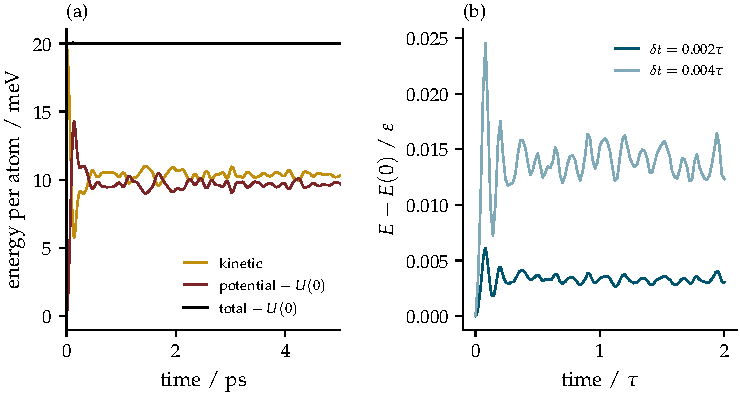
\includegraphics{ch10_code/run}
\caption{Two periodic runs. (a) 500 argon atoms started on their
face-centred cubic lattice with \SI{0.02}{\electronvolt} of kinetic energy
per atom, $\dt = \SI{10}{\femto\second}$: the kinetic energy, the potential
energy and the total, each per atom and the last two less the starting
potential energy, over the first \SI{5}{\pico\second} of
\SI{20}{\pico\second}. (b) The model salt of 64 ions with Ewald
electrostatics: the change of the total energy over $2\tau$ with $\dt =
0.002\tau$ and $0.004\tau$.}
\label{fig:md-run}
\end{figure}

\Cref{fig:md-run}(b) runs a model salt, chosen to exercise the Ewald sum
in a loop. Its 64 ions, of charge $\pm1$ and mass 1 in reduced units, sit
on a rock-salt lattice, repel each other at contact through the
Lennard-Jones energy cut off at its minimum, $2^{1/6}\sigma$, and shifted
there to zero, and attract and repel through the Coulomb energy with
$k_{\mathrm e} = 10\,\varepsilon\sigma$, a value chosen for this model,
summed by \texttt{EwaldModel}. Its energy is least with neighbouring ions
$1.0908\sigma$ apart, at $-15.810\varepsilon$ per ion pair, found as for
argon. Given $0.5\varepsilon$ of kinetic energy per ion and followed for
$2\tau$, the total energy of the 64 ions spreads by $\num{6.08e-3}\,\varepsilon$ with $\dt =
0.002\tau$ and by $\num{2.46e-2}\,\varepsilon$ with $0.004\tau$, a ratio of
4.04 for a doubled step: the $\dt^2$ of \cref{sec:in-stability}, the
test that the Ewald forces are the slopes of the Ewald energy and are
smooth.

\begin{keyidea}
A model returns the energy and the forces; the loop is velocity Verlet
over it with one call per step. The code agrees with ASE to the rounding
of the arithmetic once both use the same constants, keeps the energy of a
periodic crystal with a fluctuation 0.3\% of that of its kinetic energy
and its momentum to rounding, and its Ewald forces pass the $\dt^2$ test.
\end{keyidea}

\notebook{10}{plot the argon and model-salt runs, check the loop against ASE, and read a trajectory file back}

\begin{selfcheck}
With $\dt = \SI{10}{\femto\second}$, how many steps are 20\,ps, and how
many force calls did the argon run make, counting the first?
\end{selfcheck}

%=============================================================================!
% 10.7  MAKING IT FAST                                                        !
%=============================================================================!
\section{Making it fast}
\label{sec:md-speed}

A run of a million steps calls the model a million times, and the time a
call takes decides what can be simulated. This section measures where the
time goes and rewrites one force loop in three faster ways, each checked
against the plain one.

\subsection*{The profile}

A profiler records how long a program spends in each of its functions.
Python's \texttt{cProfile}, run on 200 steps of 4000 Lennard-Jones atoms
in reduced units with the NumPy pair model of \cref{sec:md-loop}, finds
three quarters of the time inside the neighbour list: 36\% in its 14
rebuilds by the cell list, whose loops over small cells are written in
Python, and 38\% in picking out at every step the listed pairs now within
$r_{\mathrm c}$, which reduces each of them to its nearest copy by solving
$\vb{h}\vb{s} = \vb{d}$ although the cell is a cube. The forces take most
of the remaining quarter, \texttt{np.add.at} alone 16\%. The first gains
would come from the neighbour list.

\subsection*{One loop, four ways}

The force loop runs over every pair at every step, and it shows the
choices well. A processor runs only machine code, its own short list of
simple instructions. A compiler can translate a numerical loop into machine code before it
runs. In the ordinary Python loop, the interpreter instead carries out
Python operations at each iteration, including the work needed to handle
objects and call NumPy functions. The kernel takes the
positions, the side lengths of a rectangular box and a list of pairs, and
returns the Lennard-Jones energy, shifted to zero at $r_{\mathrm c}$, and
the forces. \texttt{mdlab.kernels} has it four times:
\begin{itemize}
\item \texttt{lj\_loop}, a plain Python loop over the pairs;
\item \texttt{lj\_numpy}, the same arithmetic on whole arrays, every pair
   in each operation;
\item \texttt{lj\_numba}, the same loop with the three components of
   each pair written as a loop of their own, compiled to machine code by
   Numba when it is first called;
\item \texttt{lj\_fortran}, the loop written in Fortran and compiled
   through NumPy's \texttt{f2py}, which builds the code that lets Python
   call it.
\end{itemize}
The Fortran loop over the pairs is

\begin{code}[language={[95]Fortran}]
do p = 1, n_pairs
   i   = pair_i(p) + 1
   j   = pair_j(p) + 1
   sep = positions(:, j) - positions(:, i)
   sep = sep - box * anint(sep / box)
   r2  = sum(sep * sep)
   if (r2 >= r_cut2) cycle
   s6           = (sigma2 / r2)**3
   push         = 24.0_dp * well_depth * (2.0_dp * s6 * s6 - s6) / r2
   energy       = energy + 4.0_dp * well_depth * (s6 * s6 - s6)        &
                  - phi_cut
   forces(:, i) = forces(:, i) - push * sep
   forces(:, j) = forces(:, j) + push * sep
end do
\end{code}

\noindent Fortran counts from 1 where Python counts from 0, hence the
$+1$ of lines 2 and 3; \texttt{anint} rounds to the nearest whole number,
the minimum image of \cref{sec:md-image} in a rectangular box; and the
array \texttt{positions(3, n\_atoms)} holds one atom per column. Fortran
stores an array column after column and NumPy row after row, so both keep
the numbers in memory in the order $x_1, y_1, z_1, x_2, \dots$, and NumPy's
array of one atom per row, passed as its transpose, reaches Fortran
without a copy. \texttt{push} is $-\varphi'(r)/r$, so the force on $j$ is
\texttt{push} times the separation and the force on $i$ its opposite;
\texttt{push} times the separation is thus the opposite of the
\texttt{push} of \texttt{PairModel} in \cref{sec:md-loop}, which was the
force on $i$. The Numba version follows the Python loop with each
operation on three numbers written as a loop over the components, as in
the Fortran.

\Cref{fig:md-speed} times one call of each on atoms on a simple cubic
grid shaken by $0.05\sigma$, at $\rho = 0.8\sigma^{-3}$, with the pairs
within $r_{\mathrm c} + 0.3\sigma$ listed.
At $N = 2000$, with 74\,684 listed pairs, the plain loop takes
\SI{172}{\milli\second}, NumPy \SI{5.2}{\milli\second}, Numba
\SI{0.34}{\milli\second} and Fortran \SI{0.28}{\milli\second}: NumPy is 33
times faster than the loop, and the two compiled versions another 15 and
18 times faster than NumPy. Every version grows roughly as $N$, with the
number of listed pairs, the compiled ones less evenly. All three agree with the plain loop to about a part in $10^{12}$ in
the energy and to $\num{3e-12}$ in forces as large as 1024, in reduced
units, the differences of rounding in a different order.

\begin{figure}[htb]
\centering
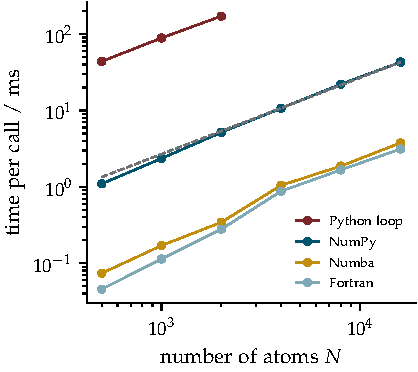
\includegraphics{ch10_code/speed}
\caption{The time of one call of the Lennard-Jones force kernel against
$N$, for atoms on a simple cubic grid shaken by $0.05\sigma$ at $\rho =
0.8\sigma^{-3}$, with $r_{\mathrm c} = 2.5\sigma$, written as a plain
Python loop, with NumPy, with Numba and in Fortran, with a line of slope 1
(dashed). Each time is the best of five, on one thread, one sequence of
instructions on one core of the processor.}
\label{fig:md-speed}
\end{figure}

The reasons are in how each runs. The plain loop takes
$\SI{172}{\milli\second}/74\,684 = \SI{2.3}{\micro\second}$ for each
pair, and the Fortran loop \SI{3.7}{\nano\second} for the same
arithmetic, so almost all of the plain loop's time goes on something other
than arithmetic: each pair makes about a dozen calls of NumPy on arrays of
three numbers, and every call first finds out what its operands are and
makes a new array for its result. NumPy on whole arrays makes those
decisions once per operation for all the pairs and does the arithmetic in
compiled code, but it passes over the pairs once for every operation,
writing a new array each time. A compiled loop keeps each pair's few
numbers in the processor's registers, its fastest storage, and touches
memory only for the indices, positions and forces.

\begin{practice}
The profile comes before any rewriting: here the slow part was the
neighbour list. Only the loop that dominates is rewritten, the plain
version is kept as the reference, and every fast version is checked
against it, as the tests of \texttt{mdlab} do. Numba compiles a Python
loop with few changes once every operation on a small array is written as
a loop over its numbers, as in \texttt{lj\_numba}; the Fortran loop took
18\% less time here.
\end{practice}

\begin{keyidea}
A profiler shows where the time goes, and in this code it was the
neighbour list. The force loop written in Python, with NumPy on each pair,
is hundreds of times slower than the loop compiled by Numba or written in
Fortran; NumPy on whole arrays lies between. Every fast version is checked
against the plain one to the rounding of the arithmetic.
\end{keyidea}

\notebook{10}{race the four kernels}

\begin{selfcheck}
At \SI{0.2}{\micro\second} per atom per call, how long does the force
kernel alone take for \SI{1}{\nano\second} of $10^4$ atoms with $\dt =
\SI{1}{\femto\second}$?
\end{selfcheck}

%=============================================================================!
% 10.S  WHAT WE NOW HAVE                                                      !
%=============================================================================!
\unnumbered{What we now have}

A sample small enough to simulate is mostly surface, and repeating a cell
of atoms in every direction removes the surface. The cell is the matrix
$\vb{h}$ of its lattice vectors; fractional coordinates $\vb{s} =
\vb{h}^{-1}\vb{r}$ wrap positions into it and, rounded, give the nearest
copy of a separation, in any cell, for every separation shorter than half
the smallest perpendicular width $w_{\min}$, the least of widths such as
$V/\lvert\vb{b}\times\vb{c}\rvert$, which bounds the cutoff.

Charges in a periodic cell need the Ewald sum: $1/r$
split by Gaussian integrals into a short-ranged part summed over near
copies and a smooth part summed as a Fourier series over the reciprocal
vectors, less the self term, with the $\vb{G} = \vb{0}$ term dropped for
a neutral cell; it reproduces the Madelung constant of rock salt for any
splitting and any equivalent cell.

Cell lists find the pairs within the
cutoff at a cost that grows as $N$, and Verlet lists with a skin reuse
them until an atom has moved half the skin. A run starts from a crystal
at its model's own spacing, with random velocities stripped of drift, and
the loop is velocity Verlet over a model that returns energy and forces.
The code agrees with ASE to the rounding of the arithmetic once both use
the same physical constants, conserves energy and momentum in a periodic
box, and passes the $\dt^2$ test with Ewald forces. A profiler found the
time in the neighbour list; the force loop, compiled by Numba or written
in Fortran, runs hundreds of times faster than the Python loop that does
each pair's arithmetic with NumPy, and agrees with it to rounding.

Chapter~11 holds the fastest vibrations fixed with constraints, so that
the step can be longer, and splits the forces by how fast they change.

%=============================================================================!
% 10.A  ANSWERS TO THE CHECKS                                                 !
%=============================================================================!
\unnumbered{Answers to the checks}
\label{sec:md-answers}

\answerto{sec:md-periodic}$\vb{s} = (9/4, -1/5, 3/6) = (2.25, -0.2,
0.5)$. Wrapping removes the floors 2, $-1$ and 0, leaving $(0.25, 0.8,
0.5)$, so the atom is put at $(1, 4, 3)$\,\AA.

\answerto{sec:md-image}No. In a cubic cell rounding does return the
nearest copy, but half the side is \SI{10}{\angstrom}, less than the
cutoff, so a pair can have a second copy within \SI{12}{\angstrom}, as
$(\pm10, 0, 0)$\,\AA\ do, and rounding misses it. By \cref{eq:md-rule}
the side must be at least \SI{24}{\angstrom}.

\answerto{sec:md-ewald}$\sqrt{-\ln10^{-8}} = 4.292$, so $r_{\mathrm c} =
4.292/0.3 = \SI{14.31}{\angstrom}$ and $G_{\mathrm c} = 2\times0.3\times
4.292 = \SI{2.575}{\per\angstrom}$.

\answerto{sec:md-neighbours}Half the skin, $0.15\sigma$. The list holds the
pairs within $2.8\sigma$: $\frac12\times\frac43\pi(2.8)^3\times0.8 = 36.8$
per atom.

\answerto{sec:md-start}$4\times125 = 500$ atoms, in a cube of side
$5\times5.267 = \SI{26.34}{\angstrom}$.

\answerto{sec:md-loop}$20\,000/10 = 2000$ steps, and 2001 force calls:
one before the first step and one in each step.

\answerto{sec:md-speed}$10^6$ steps of $10^4\times\SI{0.2}{\micro\second}
= \SI{2}{\milli\second}$ each: \SI{2000}{\second}, about half an hour.

%=============================================================================!
% 10.E  EXERCISES                                                             !
%=============================================================================!
\unnumbered{Exercises}
\label{sec:md-exercises}

The exercises run from questions of understanding, through calculations,
to short derivations marked `show that'. Full solutions are in
\hyperref[sec:md-solutions]{`Solutions to the exercises'} at the end of
the book, and Notebook~10 checks every numerical answer.

\begin{exercise}[a large enough sample]
\label{ex:md-surface}
How many atoms must a cube of $n^3$ atoms hold before fewer than 1\% of
them are on its surface?
\end{exercise}

\begin{exercise}[fractional coordinates in graphite]
\label{ex:md-fractional}
Graphite's cell has $\vb{a} = (a, 0, 0)$, $\vb{b} = (-\frac12a,
\frac{\sqrt3}2a, 0)$ and $\vb{c} = (0, 0, c)$. Find the fractional
coordinates of $\vb{r} = (\frac12a, \frac{\sqrt3}2a, \frac14c)$, and the
position to which wrapping moves it.
\end{exercise}

\begin{exercise}[graphite's volume and widths]
\label{ex:md-graphite}
Show that graphite's cell has volume $\frac{\sqrt3}2a^2c$ and
perpendicular widths $\frac{\sqrt3}2a$, $\frac{\sqrt3}2a$ and $c$, and
evaluate them for $a = \SI{2.464}{\angstrom}$ and $c =
\SI{6.711}{\angstrom}$.
\end{exercise}

\begin{exercise}[the primitive cell of a face-centred lattice]
\label{ex:md-primitive}
The face-centred cubic lattice also has a cell of one atom, with $\vb{a} =
\frac12a_0(0, 1, 1)$, $\vb{b} = \frac12a_0(1, 0, 1)$ and $\vb{c} =
\frac12a_0(1, 1, 0)$. Find its volume and its perpendicular widths, and
the largest cutoff a single such cell allows for $a_0 =
\SI{5.267}{\angstrom}$.
\end{exercise}

\begin{exercise}[rounding in a rectangular cell]
\label{ex:md-round}
In the cell with sides 2, 3 and \SI{4}{\angstrom} along the axes, find the
nearest copy of $\vb{d} = (1.8, -2.9, 0.1)$\,\AA\ by rounding, and check
that no other copy is shorter.
\end{exercise}

\begin{exercise}[a normalised Gaussian]
\label{ex:md-normal}
Show that $\int_{-\infty}^{\infty}\mathrm{e}^{-(x - x_0)^2/(2s^2)}\,\dd x
= s\sqrt{2\pi}$ for any $x_0$ and any $s > 0$.
\end{exercise}

\begin{exercise}[the error function near zero]
\label{ex:md-erf}
From the Taylor series of $\mathrm{e}^{-u^2}$, show that
$\operatorname{erf}(x) = (2/\sqrt\pi)(x - x^3/3 + \dotsb)$, and hence that
$\operatorname{erf}(\alpha r)/r$ tends to $2\alpha/\sqrt\pi$ as $r \to 0$.
\end{exercise}

\begin{exercise}[waves that do not mix]
\label{ex:md-orthogonal}
Show that the average over one period $L$ of $\cos(2\pi mx/L)\cos(2\pi
m'x/L)$, for $m$ and $m'$ among $0, 1, 2, \dots$ and not both zero, is
$\frac12$ if $m = m'$ and zero if $m \neq m'$.
\end{exercise}

\begin{exercise}[graphite's reciprocal vectors]
\label{ex:md-reciprocal}
Show that the reciprocal vectors of graphite's cell are $\vb{a}^* =
\frac{2\pi}{a}(1, \frac1{\sqrt3}, 0)$, $\vb{b}^* = \frac{2\pi}{a}(0,
\frac2{\sqrt3}, 0)$ and $\vb{c}^* = \frac{2\pi}{c}(0, 0, 1)$, and find
their lengths for $a = \SI{2.464}{\angstrom}$ and $c =
\SI{6.711}{\angstrom}$.
\end{exercise}

\begin{exercise}[the Ewald forces]
\label{ex:md-forces}
Show that the reciprocal-space force on atom $i$ is
\begin{equation*}
   \vb{F}_i = \frac{4\pi k_{\mathrm e}}{V}\,q_i\sum_{\vb{G}\neq\vb{0}}
   \frac{\mathrm{e}^{-G^2/(4\alpha^2)}}{G^2}\,\vb{G}\,\bigl[\mathcal{C}(\vb{G})
   \sin(\vb{G}\cdot\vb{r}_i) - \mathcal{S}(\vb{G})\cos(\vb{G}\cdot\vb{r}_i)\bigr] ,
\end{equation*}
and that the real-space pair term $k_{\mathrm e}q_iq_j\operatorname{erfc}
(\alpha r)/r$ has the slope $-k_{\mathrm e}q_iq_j[\operatorname{erfc}(\alpha
r)/r + (2\alpha/\sqrt\pi)\,\mathrm{e}^{-\alpha^2r^2}]/r$.
\end{exercise}

\begin{exercise}[the waves of rock salt]
\label{ex:md-rocksalt}
Rock salt in its cubic cell of side 2, with $d = 1$, has cations at $(0,
0, 0)$, $(0, 1, 1)$, $(1, 0, 1)$ and $(1, 1, 0)$ and anions shifted from
them by $(1, 0, 0)$. Show that its waves are $\vb{G} = \pi(m_1, m_2,
m_3)$, that $\mathcal{S}(\vb{G}) = 0$ for all of them, and that $\mathcal{C}(\vb{G}) = 8$
when $m_1$, $m_2$ and $m_3$ are all odd and zero otherwise.
\end{exercise}

\begin{exercise}[the cost of Ewald]
\label{ex:md-cost}
At fixed density $\rho = N/V$, the real-space sum costs about $N$ times
the number of copies within $r_{\mathrm c} \propto 1/\alpha$, and the
reciprocal sum $N$ times the number of waves within $G_{\mathrm c}
\propto \alpha$. Show that the cheapest $\alpha$ is proportional to
$(N/V^2)^{1/6}$ and that the total cost then grows as $N^{3/2}$.
\end{exercise}

\begin{exercise}[choosing the Ewald parameters]
\label{ex:md-parameters}
For 1000 ions in a cubic cell of side \SI{30}{\angstrom}, with
$\epsilon_{\mathrm E} = 10^{-6}$ and the real-space cutoff at half the
side, find $\alpha$, $G_{\mathrm c}$ and roughly how many waves the
reciprocal sum needs.
\end{exercise}

\begin{exercise}[neighbours in water]
\label{ex:md-water}
Liquid water holds about 0.0334 molecules per \AA$^3$. How many molecules
lie within \SI{10}{\angstrom} of a given one?
\end{exercise}

\begin{exercise}[counting small cells]
\label{ex:md-cells}
With $r_{\mathrm c} + r_{\mathrm{skin}} = \SI{9.5}{\angstrom}$, how many small
cells does a cell list use in cubes of side 40, 30 and
\SI{25}{\angstrom}, and in which does \texttt{mdlab} test all pairs
instead?
\end{exercise}

\begin{exercise}[how often to rebuild]
\label{ex:md-rebuild}
Argon atoms with \SI{0.0104}{\electronvolt} of kinetic energy each move
at a root-mean-square speed $\sqrt{2K/m}$, with the factor of
\cref{eq:en-mv2} to put it in \si{\angstrom\per\femto\second}. How many
steps of
\SI{10}{\femto\second} does such an atom take to move half a skin of
\SI{1}{\angstrom}, and why does the run of \cref{sec:md-loop} rebuild its
list about twice as often?
\end{exercise}

\begin{exercise}[no drift]
\label{ex:md-drift}
Show that subtracting $\vb{P}/M$ from every velocity leaves the total
momentum zero, and that multiplying every velocity by one factor then
keeps it zero.
\end{exercise}

\begin{exercise}[half the energy]
\label{ex:md-half}
A single harmonic vibration is started at its minimum with kinetic energy
$K_0$. Show that its kinetic energy averages $\frac12K_0$ over a period.
\end{exercise}

\begin{exercise}[two femtoseconds]
\label{ex:md-femtosecond}
ASE's femtosecond differs from \texttt{mdlab}'s by 4.6 parts in $10^9$.
Roughly how far apart would two runs of \SI{1000}{\femto\second} put an
atom moving at \SI{0.0031}{\angstrom\per\femto\second}, and how does this
compare with the $\num{1.6e-8}$\,\AA\ of \cref{sec:md-loop}?
\end{exercise}


%=============================================================================!
% CHAPTER 11  CONSTRAINTS AND MULTIPLE TIME STEPS                             !
%=============================================================================!
\chapter{Constraints and multiple time steps}
\label{ch:constraints}

%=============================================================================!
% 11.0  CHAPTER OPENING                                                       !
%=============================================================================!
The code of Chapter~10 advances every atom with the same step. Chapter~9
showed why that step must be short compared with the fastest vibration:
in water, an oxygen--hydrogen bond stretches with a period of about
\SI{9}{\femto\second}, restricting the step to around
\SI{0.5}{\femto\second}. Molecular rotation and rearrangement take
picoseconds, so resolving the bond vibration requires thousands of steps
to follow these slower motions.

We examine three ways to reduce that cost. Holding bonds at fixed lengths
removes their vibrations; SHAKE and RATTLE calculate the constraint forces
needed at each step. Splitting fast and slow forces allows the costly
slow forces to be evaluated less often, although resonance limits the
outer step. Moving some mass from the heavy atoms to their hydrogens
slows the fastest vibrations without changing the potential energy. We
compare these choices on a box of water and use its trajectories to
identify their limits and common implementation faults. The constraints
also change the number of degrees of freedom, which Chapter~12 needs to
relate kinetic energy to temperature.

%=============================================================================!
% 11.1  HOLDING A BOND FIXED                                                  !
%=============================================================================!
\section{Holding a bond fixed}
\label{sec:cs-shake}

The fastest motions in most molecules are the stretches of bonds to
hydrogen (\cref{tab:os-vibrations}), and \cref{sec:pe-classical} found
them thoroughly quantum: for the O--H stretch of water $\hbar\omega$ is
17.5 times $\kB T$ at room temperature, so a simulation with classical
nuclei gets the energy of this vibration wrong whatever its step. Yet the
same vibration, with its period of \SI{9}{\femto\second}, is what holds
the step down. Replacing each such bond by a rod of fixed length
(\cref{sec:la-multipliers}) removes the vibration altogether. The bond
between atoms $i$ and $j$, held at the length $d$, is the constraint
\begin{equation*}
   \chi = \tfrac12\bigl(\lvert\vb{r}_{ij}\rvert^2 - d^2\bigr) = 0 ,
   \qquad \vb{r}_{ij} = \vb{r}_j - \vb{r}_i ,
\end{equation*}
whose force, found in \cref{sec:la-multipliers}, is $\lambda\vb{r}_{ij}$
on atom $j$ and $-\lambda\vb{r}_{ij}$ on atom $i$: along the bond, equal
and opposite, with a size set by the multiplier $\lambda$. This section
finds $\lambda$ at every step.

\subsection*{The constrained step}

The Störmer--Verlet step of \cref{eq:in-stormer}, written for atom $i$
with its force $\vb{F}_i$ and the constraint force $\vb{F}_i^{\mathrm c}$
added, is
\begin{equation*}
   \vb{r}_i(t + \dt) = 2\vb{r}_i(t) - \vb{r}_i(t - \dt)
   + \frac{\dt^2}{m_i}\bigl(\vb{F}_i + \vb{F}_i^{\mathrm c}\bigr) .
\end{equation*}
Without the constraint the atom would go to the provisional position
$\tilde{\vb{r}}_i = 2\vb{r}_i(t) - \vb{r}_i(t - \dt) +
(\dt^2/m_i)\vb{F}_i$, so the constrained step is the provisional one
corrected, $\vb{r}_i(t + \dt) = \tilde{\vb{r}}_i +
(\dt^2/m_i)\vb{F}_i^{\mathrm c}$. With one bond, and its force taken at
time $t$, the two atoms move to
\begin{align*}
   \vb{r}_j(t + \dt) &= \tilde{\vb{r}}_j
      + \frac{\dt^2\lambda}{m_j}\,\vb{r}_{ij} ,\\
   \vb{r}_i(t + \dt) &= \tilde{\vb{r}}_i
      - \frac{\dt^2\lambda}{m_i}\,\vb{r}_{ij} ,
\end{align*}
with $\vb{r}_{ij}$ the bond at time $t$. Subtracting the second line from
the first, the bond at $t + \dt$ is
\begin{align*}
   \vb{r}_{ij}(t + \dt)
   &= \tilde{\vb{r}}_{ij} + \dt^2\lambda\Bigl(\frac{1}{m_i}
      + \frac{1}{m_j}\Bigr)\vb{r}_{ij}\\
   &= \tilde{\vb{r}}_{ij} + \eta\,\vb{r}_{ij} ,
   \qquad \eta = \frac{\dt^2\lambda}{m_{\mathrm r}} ,
   && \text{$\frac1{m_i} + \frac1{m_j} = \frac{m_i + m_j}{m_im_j}
      = \frac{1}{m_{\mathrm r}}$,}
\end{align*}
where $\tilde{\vb{r}}_{ij} = \tilde{\vb{r}}_j - \tilde{\vb{r}}_i$ is the
provisional bond and $m_{\mathrm r}$ the reduced mass of
\cref{sec:os-bodies}. The new bond is the provisional one plus a multiple
of the old, as \cref{fig:cs-shake-geometry} draws. The constraint must
hold at $t + \dt$, $\lvert\tilde{\vb{r}}_{ij} + \eta\vb{r}_{ij}\rvert^2 =
d^2$. Expanding the square as $(\vb{a} + \vb{s})\cdot(\vb{a} + \vb{s})$
was expanded in \cref{sec:ro-freedom} gives $\lvert\tilde{\vb{r}}_{ij}
\rvert^2 + 2\eta\,\tilde{\vb{r}}_{ij}\cdot\vb{r}_{ij} + \eta^2\lvert
\vb{r}_{ij}\rvert^2 = d^2$, and with $\lvert\vb{r}_{ij}\rvert^2 = d^2$,
since the bond held at $t$,
\begin{equation}
   d^2\eta^2 + 2\,(\tilde{\vb{r}}_{ij}\cdot\vb{r}_{ij})\,\eta
   + \lvert\tilde{\vb{r}}_{ij}\rvert^2 - d^2 = 0 ,
   \label{eq:cs-quadratic}
\end{equation}
a quadratic equation for the one unknown $\eta$.

\begin{figure}[htb]
\centering
\begin{tikzpicture}[line cap=round, line join=round, scale=1.45,
   old/.style={circle, draw=black, fill=white, inner sep=1.8pt},
   trial/.style={circle, draw=black!45, fill=black!20, inner sep=1.8pt},
   new/.style={circle, fill=black, inner sep=1.8pt},
   arr/.style={-{Stealth[length=5pt]}, line width=0.8pt}]
   \draw[arr, black!60] (0,0) -- (3,0)
      node[midway, below] {$\vb{r}_{ij}$};
   \draw[black!45, dashed] (0.2,0.9) -- (4.0,1.5)
      node[pos=0.5, above=2pt, black!60] {$\tilde{\vb{r}}_{ij}$};
   \draw[line width=1pt] (0.8455,0.9) -- (3.7848,1.5);
   \draw[arr, accent] (0.2,0.9) -- (0.8455,0.9);
   \draw[arr, accent] (4.0,1.5) -- (3.7848,1.5);
   \node[old, label={below:$\vb{r}_i(t)$}] at (0,0) {};
   \node[old, label={below:$\vb{r}_j(t)$}] at (3,0) {};
   \node[trial, label={left:$\tilde{\vb{r}}_i$}] at (0.2,0.9) {};
   \node[trial, label={right:$\tilde{\vb{r}}_j$}] at (4.0,1.5) {};
   \node[new, label={below:$\vb{r}_i(t + \dt)$}] at (0.8455,0.9) {};
   \node[new, label={above:$\vb{r}_j(t + \dt)$}] at (3.7848,1.5) {};
\end{tikzpicture}
\caption{One step of a bond held at the length $d$, here 3. Atoms $i$
(mass 1) and $j$ (mass 3) start at the open circles. Without the
constraint they would reach the grey provisional positions, a bond
$\tilde{\vb{r}}_{ij}$ too long (dashed); the correction (arrows) moves
each along the old bond $\vb{r}_{ij}$, the lighter atom three times as
far, to the black positions, where the bond has length 3 again.}
\label{fig:cs-shake-geometry}
\end{figure}

\subsection*{One bond}

Two atoms, $i$ of mass 1 and $j$ of mass 3, joined by a bond of length 1
along $x$, drift apart to
1.2 in a step, so $\vb{r}_{ij} = (1, 0, 0)$, $\tilde{\vb{r}}_{ij} = (1.2,
0, 0)$, $\tilde{\vb{r}}_{ij}\cdot\vb{r}_{ij} = 1.2$ and
$\lvert\tilde{\vb{r}}_{ij}\rvert^2 - d^2 = 0.44$:
\begin{align*}
   \eta^2 + 2.4\,\eta + 0.44 &= 0 ,\\
   \eta &= \frac{-2.4 \pm \sqrt{2.4^2 - 4\times0.44}}{2}
   = -1.2 \pm 1 ,
   && \text{the quadratic formula,}
\end{align*}
so $\eta = -0.2$ or $-2.2$. The first shortens the bond to $1.2 - 0.2 =
1$. The second gives $1.2 - 2.2 = -1$, the bond turned round, a solution
of the equation that no short step can reach: as $\dt$ shrinks,
$\tilde{\vb{r}}_{ij}$ approaches $\vb{r}_{ij}$ and the correction must
vanish, which only the root nearer zero does: with $\tilde{\vb{r}}_{ij} =
\vb{r}_{ij}$, \cref{eq:cs-quadratic} becomes $d^2\eta^2 + 2d^2\eta = 0$,
with roots 0 and $-2$. With $\eta = -0.2$ and
$m_{\mathrm r} = 1\times3/(1 + 3) = 0.75$, atom $j$ moves by
$\dt^2\lambda/m_j = \eta m_{\mathrm r}/m_j = -0.05$ along the bond and atom
$i$ by $+0.15$: the lighter atom moves three times as far, and the centre
of mass, $1\times0.15 + 3\times(-0.05) = 0$, does not move at all.

The quadratic has real roots only if the number under the square root of
the quadratic formula, $4(\tilde{\vb{r}}_{ij}\cdot\vb{r}_{ij})^2 -
4d^2(\lvert\tilde{\vb{r}}_{ij}\rvert^2 - d^2)$, is not negative, that is,
if $(\tilde{\vb{r}}_{ij}\cdot\vb{r}_{ij})^2 \ge d^2(\lvert\tilde{\vb{r}}_{ij}
\rvert^2 - d^2)$. Writing
$\phi$ for the angle between the provisional and the old bond, so that
$\tilde{\vb{r}}_{ij}\cdot\vb{r}_{ij} = \lvert\tilde{\vb{r}}_{ij}\rvert
\,d\cos\phi$, and dividing by $d^2$, the condition reads
$\lvert\tilde{\vb{r}}_{ij}\rvert^2\cos^2\phi \ge \lvert\tilde{\vb{r}}_{ij}
\rvert^2 - d^2$, that is, $d^2 \ge \lvert\tilde{\vb{r}}_{ij}\rvert^2(1 -
\cos^2\phi) = \lvert\tilde{\vb{r}}_{ij}\rvert^2\sin^2\phi$, or, taking
square roots, $\lvert\tilde{\vb{r}}_{ij}\rvert\sin\phi \le d$. The part of the provisional bond at
right angles to the old one must be no longer than the bond: a correction
along the old bond cannot shorten that part. A bond stretched by 50\% and
turned in one step by more than $\arcsin(1/1.5) = \ang{41.8}$, and less
than $\ang{180} - \ang{41.8} = \ang{138.2}$, where $\sin\phi$ is again
$1/1.5$, cannot be corrected at all, a sign of a step far too long.

\subsection*{Many bonds}

The bonds of a molecule share atoms. The three distances held in a rigid
water molecule join its three atoms in a triangle, and moving two atoms to
correct one distance changes the other two, so the quadratics of the three
bonds are coupled. Ryckaert, Ciccotti and Berendsen avoided solving them
together\cite{Ryckaert1977}: their method, SHAKE, corrects the bonds one
at a time, each by an approximate solution of its own equation with the
others' atoms where they are, and sweeps through all the bonds again and
again until every one holds. The approximation drops the $\eta^2$ of
\cref{eq:cs-quadratic}, which is small for a short step:
\begin{equation}
   \eta \approx \frac{d^2 - \lvert\tilde{\vb{r}}_{ij}\rvert^2}
   {2\,\tilde{\vb{r}}_{ij}\cdot\vb{r}_{ij}} .
   \label{eq:cs-linear}
\end{equation}
For the example this gives $-0.44/2.4 = -0.1833$, and the bond becomes
1.0167 long. Applied again, with the corrected bond in place of
$\tilde{\vb{r}}_{ij}$ and $\vb{r}_{ij}$ still the old bond, it gives
$-0.0165$, and
the bond is $1.000137$. The repeated step is a method for solving any
equation.

\begin{toolbox}[Newton's method]
To solve $f(y) = 0$, we start from a guess $y_n$ and replace the curve
$f(y)$ near it by its tangent, the first two terms of its Taylor series
(\cref{sec:mo-taylor}), $f(y_n) + f'(y_n)(y - y_n)$. The tangent is zero at
\begin{equation*}
   y_{n+1} = y_n - \frac{f(y_n)}{f'(y_n)} ,
\end{equation*}
the next guess. To see how fast the guesses close in, we write the root
as $y^*$ and the error as $e_n = y_n - y^*$, and expand $f(y^*)$ about
$y_n$, with $y^* - y_n = -e_n$:
\begin{align*}
   0 = f(y^*) &= f(y_n) - e_nf'(y_n) + \tfrac12e_n^2f''(y_n)
   + \order{e_n^3} ,\\
   \frac{f(y_n)}{f'(y_n)} &= e_n - \frac{f''(y_n)}{2f'(y_n)}\,e_n^2
   + \order{e_n^3} ,
\end{align*}
the second line by dividing the first by $f'(y_n)$ and rearranging.
Subtracting $y^*$ from both sides of the rule gives $e_{n+1} = e_n -
f(y_n)/f'(y_n)$, and so
\begin{equation*}
   e_{n+1} = \frac{f''(y_n)}{2f'(y_n)}\,e_n^2 + \order{e_n^3} .
\end{equation*}
Each error is about a fixed multiple of the square of the one before, so
once the error is small the number of correct digits roughly doubles at
every step. For $f(y) = y^2 - 2$ from $y_0 = 1$, the guesses $1.5$,
$1.4166667$, $1.4142157$ and $1.4142135624$ have errors of $0.086$,
$0.0025$, $\num{2.1e-6}$ and $\num{1.6e-12}$ against $\sqrt2$. The method
needs $f'(y_n) \neq 0$ and a start close enough to the root; far from it,
the tangent can point anywhere.
\end{toolbox}

For one bond, $f(\eta) = \lvert\tilde{\vb{r}}_{ij} +
\eta\vb{r}_{ij}\rvert^2 - d^2$, the left side of \cref{eq:cs-quadratic},
so $f'(\eta) = 2d^2\eta + 2\,\tilde{\vb{r}}_{ij}\cdot\vb{r}_{ij} =
2\,\vb{r}_{ij}\cdot(\tilde{\vb{r}}_{ij} + \eta\vb{r}_{ij})$,
which at $\eta = 0$ is $2\,\tilde{\vb{r}}_{ij}\cdot\vb{r}_{ij}$, so
\cref{eq:cs-linear} is the first step of Newton's method from $\eta = 0$.
Once the atoms have moved, the corrected bond takes the place of
$\tilde{\vb{r}}_{ij}$, and the same formula is the next step. Here
$f''(\eta) = 2d^2$ and, near the root, $f'(\eta)$ is twice the dot product
of the old bond with the corrected one, $2d^2\cos\theta$ if the two bonds
are $\theta$ apart, so each error in $\eta$ is $2d^2/(2\times2d^2\cos
\theta)$ times the square of the one before. An error $e$ in $\eta$ changes
the length by about $e\,d\cos\theta$, so the relative error of the length
is $1/(2\cos^2\theta)$ times the square of the one before: about half,
when the bond has not turned far. \Cref{fig:cs-shake}(a) measures it: a
bond stretched by 10\% has a relative error of 0.1, then $\num{5.0e-3}$,
$\num{1.4e-5}$ and $\num{1.1e-10}$, each 0.50 to 0.57 times the square of
the one before; the corrected bond lies \ang{19.9} off the old one, and
$1/(2\cos^2\ang{19.9}) = 0.565$.

\begin{figure}[htb]
\centering
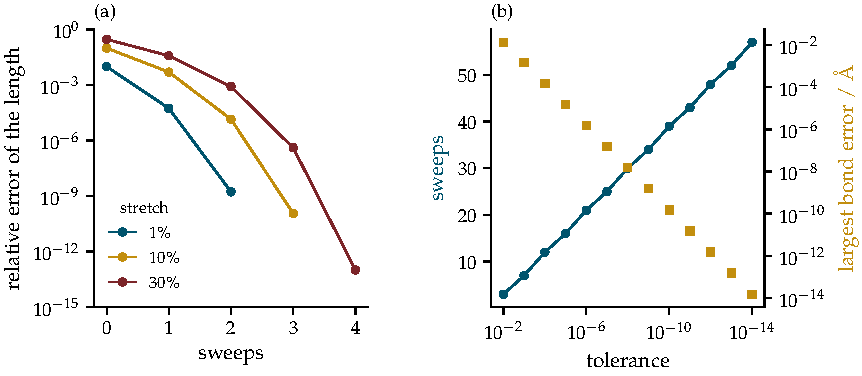
\includegraphics{ch11_constraints/shake}
\caption{How SHAKE converges. (a) One bond of length 1 between equal
masses, stretched by 1\%, 10\% and 30\% in a direction \ang{18} off the
old bond: the relative error of its length after each sweep, until it
reaches the rounding of the arithmetic. (b) The 64 rigid water molecules
of \cref{sec:cs-water} after one step of \SI{2}{\femto\second} without
constraints: the sweeps needed against the tolerance (circles) and the
largest error of a held distance that is left (squares, right axis).}
\label{fig:cs-shake}
\end{figure}

The function \texttt{shake} of \texttt{mdlab.constraints} carries out the
sweeps. The bonds are sorted beforehand into groups that share no atom, so
that every bond of a group can be corrected at once with NumPy. For
water, whose bonds are listed molecule by molecule, this applies the same
corrections in the same order as taking the bonds one at a time; for other
lists two bonds that share an atom can change places within a sweep, which
changes the path of the sweeps but not the conditions they end on. The
loop is
\begin{code}
    for sweep in range(1, max_sweeps + 1):
        moved = False
        for g in groups:
            i, j = pairs[g, 0], pairs[g, 1]
            now = r[j] - r[i] + copy[g]
            eta = 0.5 * (d2[g] - np.sum(now * now, 1)) / np.sum(
                old[g] * now, 1
            )
            eta[np.abs(eta) <= tolerance] = 0.0
            moved = moved or bool(np.any(eta))
            push = (m_r[g] * eta)[:, None] * old[g]
            r[j] += push / m[j, None]
            r[i] -= push / m[i, None]
        if not moved:
            return r, sweep
\end{code}
\noindent Here \texttt{old} holds the bonds $\vb{r}_{ij}$ at time $t$,
\texttt{now} the current ones, \texttt{d2} the squared lengths and
\texttt{m\_r} the reduced masses; \texttt{push} is $m_{\mathrm r}\eta\,
\vb{r}_{ij}$, which divided by $m_j$ is atom $j$'s move. The array
\texttt{copy} holds, for each bond, the multiple of the lattice vectors
that turns $\vb{r}_j - \vb{r}_i$ into its nearest copy in the provisional
positions (\cref{sec:md-image}), so a molecule that lies across a face of the cell
is corrected as one piece. A sweep that leaves every $\lvert\eta\rvert$
below the tolerance moves nothing, and ends the loop. Since $\eta$ is
about the fraction by which a bond is too long or too short (a bond $1 +
s$ times its length along the old one gives, by \cref{eq:cs-linear}, $\eta
= -s(1 + \frac12s)/(1 + s) \approx -s$), the
tolerance is a relative error of the lengths: $10^{-10}$ in
\texttt{mdlab} unless another is asked for.

Several bonds converge more slowly than one. \Cref{fig:cs-shake}(b) takes
the box of 64 rigid water molecules of \cref{sec:cs-water} through one
step of \SI{2}{\femto\second} with no constraint, which leaves the
largest held distance in error by \SI{0.030}{\angstrom}, 3.1\% of an O--H
bond, and corrects it by SHAKE. A tolerance of $10^{-10}$ needs 39 sweeps.
Each tenfold reduction of the tolerance costs 4.5 more sweeps, so each
sweep reduces the error by a steady factor $q$ with $q^{4.5} = 10$, $q =
10^{1/4.5} = 1.67$, where a
single bond squared it: correcting one side of a triangle disturbs the
other two, and the errors are passed round it. The largest error left is
1.5 times the tolerance in \si{\angstrom}, as it should be for a relative
error of distances up to the H--H length of \SI{1.51}{\angstrom}.

\begin{keyidea}
A held bond adds a force along the old bond to the step, so the new bond
is the provisional one plus $\eta$ times the old. The constraint at the
end of the step is a quadratic in $\eta$, and its first-order solution is
a step of Newton's method. SHAKE takes the bonds one at a time with that
step, and sweeps until every bond holds to a tolerance.
\end{keyidea}

\notebook{11}{drift a bond and follow SHAKE sweep by sweep}

\begin{selfcheck}
In the example with masses 1 and 3, the masses are changed to 2 and 2.
Does $\eta$ change, and how far does each atom move?
\end{selfcheck}

%=============================================================================!
% 11.2  VELOCITIES TOO: RATTLE                                                !
%=============================================================================!
\section{Velocities too: RATTLE}
\label{sec:cs-rattle}

SHAKE corrects positions, and the Störmer--Verlet step it was built on
carries no velocities. The loop of \cref{sec:md-loop} uses velocity
Verlet, which needs the velocities at the same times as the positions,
for the kinetic energy and to start the next step. Andersen's RATTLE
gives velocity Verlet the same constraints\cite{Andersen1983}; this
section derives it, checks it against an independent code, and counts
the motions that are left.

\subsection*{Two corrections}

Velocity Verlet is a half kick, a drift and a half kick
(\cref{sec:in-splitting}). With the constraint force added to the first
half kick, the step of atom $i$ begins
\begin{align*}
   \vb{v}_i(t + \tfrac12\dt) &= \vb{v}_i(t) + \frac{\dt}{2m_i}
      \bigl(\vb{F}_i + \vb{F}_i^{\mathrm c}\bigr) ,\\
   \vb{r}_i(t + \dt) &= \vb{r}_i(t) + \dt\,\vb{v}_i(t + \tfrac12\dt)
   = \tilde{\vb{r}}_i + \frac{\dt^2}{2m_i}\,\vb{F}_i^{\mathrm c} ,
\end{align*}
with the provisional position now $\tilde{\vb{r}}_i = \vb{r}_i(t) +
\dt\,\vb{v}_i(t) + (\dt^2/2m_i)\vb{F}_i$. This has the form of the
constrained Störmer step with $\dt^2/2$ in place of $\dt^2$, a factor
that $\eta = \dt^2\lambda/(2m_{\mathrm r})$ absorbs, so \texttt{shake}
corrects the positions unchanged. The half-step velocity drove the drift,
so it must take the same correction, divided by $\dt$; equivalently,
$\vb{v}_i(t + \frac12\dt) = [\vb{r}_i(t + \dt) - \vb{r}_i(t)]/\dt$ once the
positions are corrected.

The second half kick, with the forces at the new positions, leaves
velocities that would in general stretch or shrink the bonds. The length
of a bond stays $d$ only if it is not changing, and, differentiating
component by component as for $\lvert\vb{v}\rvert^2$ in
\cref{sec:mo-circle},
\begin{equation*}
   \frac{\dd}{\dd t}\,\tfrac12\lvert\vb{r}_{ij}\rvert^2
   = \vb{r}_{ij}\cdot\vb{v}_{ij} ,
   \qquad \vb{v}_{ij} = \vb{v}_j - \vb{v}_i ,
\end{equation*}
which must be zero at $t + \dt$: the two atoms may move side by side or
turn about each other, but not approach or separate along the bond. A
second constraint force, along the new bond $\vb{r}_{ij}$, changes $\vb{v}_j$
by $(m_{\mathrm r}\zeta/m_j)\,\vb{r}_{ij}$ and $\vb{v}_i$ by
$-(m_{\mathrm r}\zeta/m_i)\,\vb{r}_{ij}$, for some number $\zeta$, so that,
as for the positions, the relative velocity changes by $m_{\mathrm
r}\zeta(1/m_j + 1/m_i)\vb{r}_{ij} = \zeta\vb{r}_{ij}$. Then
\begin{align*}
   (\vb{v}_{ij} + \zeta\vb{r}_{ij})\cdot\vb{r}_{ij} &= 0 ,\\
   \zeta &= -\frac{\vb{v}_{ij}\cdot\vb{r}_{ij}}{d^2}
   && \text{as $\lvert\vb{r}_{ij}\rvert^2 = d^2$.}
\end{align*}
This condition is linear in $\zeta$, so one correction makes a single
bond exact, and bonds that share atoms are swept until all hold, as in
SHAKE. For atom $i$ of mass 1 and atom $j$ of mass 3, joined along $x$
with $d = 1$, so that $\vb{r}_{ij} = (1, 0, 0)$, and with $\vb{v}_i =
\vb{0}$ and $\vb{v}_j = (0.3, 0.4, 0)$, $\zeta = -0.3$, and the corrected
velocities are $(0.225, 0, 0)$ and $(0.225, 0.4, 0)$: the relative motion
along the bond is gone, the sideways motion of atom $j$ is untouched.

Every correction, of positions or of velocities, changes $m_j\vb{v}_j$ by
$m_{\mathrm r}\zeta\vb{r}_{ij}$ and $m_i\vb{v}_i$ by the opposite (or the
positions likewise), so the total momentum and the centre of mass are
unchanged by the constraints, as \cref{sec:ne-bodies} requires of forces
between the atoms of a system. In the example, the momentum along $x$ is
$3\times0.3 = 0.9$ before and $0.225 + 3\times0.225 = 0.9$ after, and
along $y$ it stays $3\times0.4 = 1.2$.

The function \texttt{rattle\_step} of \texttt{mdlab.constraints} is the
whole step:
\begin{code}
    v_half = v + 0.5 * dt * force_to_accel * np.asarray(forces) / m
    r, _ = shake(r0 + dt * v_half, r0, m[:, 0], bonds, lengths, **keep)
    v_half = (r - r0) / dt
    u, f = model(r)
    v = v_half + 0.5 * dt * force_to_accel * f / m
    v, _ = rattle_velocities(r, v, m[:, 0], bonds, lengths, **keep)
    return r, v, u, f
\end{code}
\noindent with \texttt{force\_to\_accel} the factor of \cref{sec:ne-atoms}
that turns a force in \si{\electronvolt\per\angstrom} over a mass in amu
into an acceleration in \si{\angstrom\per\femto\second\squared}, and
\texttt{keep} passing on the cell and the tolerance. The model is called
once per step, as in velocity Verlet; the constraints add only the sweeps,
and for the water box of \cref{sec:cs-water} one SHAKE to a tolerance of
$10^{-10}$ after a step of \SI{2}{\femto\second} takes about a tenth of the
time of one call of the model.

Running the step forwards and then backwards from the reversed velocities
retraces it. Fifty steps of \SI{2}{\femto\second} of the water box of
\cref{sec:cs-water}, out and back with a tolerance of $10^{-14}$, recover
the starting positions to $\num{5.2e-12}$\,\AA\ and the velocities to
$\num{1.9e-13}$\,\AA/fs. Leimkuhler and Skeel showed that RATTLE, like
velocity Verlet, is symplectic for motion confined to the
constraints\cite{LeimkuhlerSkeel1994}, so its energy should stay in a
band, as \cref{sec:cs-water} measures.

\subsection*{Checked against ASE}

ASE carries out the same two corrections: its \texttt{VelocityVerlet},
given the constraint \texttt{FixBondLengths}, corrects the positions and
half-step velocities after the drift and the velocities after the second
half kick, with the update of \cref{eq:cs-linear} for the positions and
the $\zeta$ above for the velocities. Given the forces of the
\texttt{mdlab} water model, the same start and the same femtosecond
(\cref{sec:md-loop}), 50 steps of \SI{1}{\femto\second} of the box of 64
rigid molecules agree to $\num{2.1e-12}$\,\AA\ in the positions and
$\num{1.5e-13}$\,\AA/fs in the velocities, with both codes' bonds held to
$\num{1.5e-13}$\,\AA\ at a tolerance of $10^{-13}$.

\subsection*{The motions that are left}

Each independent distance constraint removes one way of moving. A system
of $N$ atoms with $n_{\mathrm c}$ independent held distances has $3N - n_{\mathrm c}$ degrees of
freedom (\cref{sec:ro-freedom,sec:la-coordinates}), and $3N - n_{\mathrm c} - 3$ once the
drift of the centre of mass is removed and kept at zero. A water molecule
with all three of its distances held has $9 - 3 = 6$: the three drifts and
three turnings of \cref{sec:ro-freedom}, and no way left to vibrate. For
64 molecules, 192 atoms, flexible water has $576 - 3 = 573$ freedoms,
water with its 128 O--H bonds held has $573 - 128 = 445$, and rigid water,
with $3\times64 = 192$ distances held, $573 - 192 = 381$.
Chapter~12 needs these counts, since the kinetic energy is shared among
the freedoms.

\begin{keyidea}
RATTLE is velocity Verlet with two corrections along the bonds: after the
drift, the positions are corrected by SHAKE and the half-step velocities
with them; after the second half kick, each relative velocity loses its
part along its bond. Both corrections keep the total momentum; the step
is reversible and symplectic, and agrees with ASE to the rounding of the
arithmetic. Each held distance removes one freedom.
\end{keyidea}

\notebook{11}{correct a pair of velocities, and run RATTLE beside ASE}

\begin{selfcheck}
Atoms of masses 2 and 2, joined along $x$ with $d = 1$, have $\vb{v}_i =
(0.1, 0, 0)$ and $\vb{v}_j = (-0.1, 0.2, 0)$. What are the velocities
after the correction?
\end{selfcheck}

%=============================================================================!
% 11.3  RIGID WATER                                                           !
%=============================================================================!
\section{Rigid water}
\label{sec:cs-water}

Holding bonds fixed is meant to lengthen the step, and how much it
lengthens it is a question of measurement. This section builds a small
box of liquid water, runs it flexible, with only its O--H bonds held, and
rigid, and compares the energy fluctuation of the three at a range of
steps by the test of \cref{sec:in-stability}.

\subsection*{A model of water}

The TIP3P model of Jorgensen and co-workers\cite{Jorgensen1983}, in the
form ASE implements it\cite{Larsen2017}, places a charge of $-0.834e$ on
each oxygen atom and $+0.417e$ on each hydrogen, gives the oxygen atoms a
Lennard-Jones energy between one another with $\sigma =
\SI{3.15061}{\angstrom}$ and $\varepsilon = \SI{6.596}{\milli\electronvolt}$
(which ASE stores as 0.1521 kilocalories per mole, a chemists' unit that
\texttt{mdlab.units} converts), and fixes the shape of the
molecule, with O--H \SI{0.9572}{\angstrom} and the H--O--H angle
\ang{104.52}, so that H--H is \SI{1.5139}{\angstrom}; ASE's own tests run
it with all three distances held by \texttt{FixBondLengths}. The charges
describe how one molecule pulls on another; the Coulomb energy of the
pairs within a molecule is left out, since the bonds stand in for it, and
would otherwise draw each hydrogen onto its own oxygen with an energy of
$k_{\mathrm e}q_{\mathrm O}q_{\mathrm H}/r = \SI{-5.2}{\electronvolt}$ at
\SI{0.9572}{\angstrom}.

The class \texttt{WaterModel} of \texttt{mdlab.water} computes the
Lennard-Jones energy between oxygen atoms, switched off smoothly between
5 and \SI{6}{\angstrom} (\cref{sec:pe-cutoffs}), and the Coulomb energy
of all the charges and their copies by the Ewald sum of
\cref{sec:md-ewald}, less the Coulomb energy of each molecule's own three
pairs. For the flexible model it adds the three springs of the spring
model of \cref{sec:ro-freedom}, $k_{\mathrm{OH}} =
\SI{48.48}{\electronvolt\per\angstrom\squared}$ along each O--H and
$k_{\mathrm{HH}} = \SI{17.66}{\electronvolt\per\angstrom\squared}$
between the hydrogens, at rest at the TIP3P shape, whose fastest
vibration, the symmetric stretch of the model, has $\omega =
\SI{0.857}{\radian\per\femto\second}$ and a period of
\SI{7.33}{\femto\second}. Its tests check the forces against differences
of the energy, for the rigid and the flexible model, and its parameters
against ASE's.

Sixty-four molecules, turned at random, are placed on a $4\times4\times4$
grid in a cube of side \SI{12.43}{\angstrom}, which gives the density of
liquid water at \SI{298.15}{\kelvin} and \SI{0.1}{\mega\pascal},
\SI{0.997}{\gram\per\centi\metre\cubed}\cite{NISTWebBook}; half the side,
\SI{6.21}{\angstrom}, exceeds the cutoff, as \cref{sec:md-image}
requires. A grid is a poor arrangement for a liquid, and the molecules
release energy as they leave it, which heats the box. The script that
prepares it therefore follows the rigid molecules for ten rounds of
\SI{1}{\pico\second} with $\dt = \SI{2}{\femto\second}$, each round
starting from new random velocities of the kind of \cref{sec:md-start},
which discard the heat the last round released,
with no drift, no part along a held bond, and a kinetic energy of
\SI{12.93}{\milli\electronvolt} for each freedom; Chapter~12 shows that
this is the share of each freedom at \SI{300}{\kelvin}. The potential
energy falls from \SI{-2.37}{\electronvolt} on the grid to
\SI{-25.70}{\electronvolt} after the tenth round, by
\SI{0.12}{\electronvolt} in that last round, a slow change whose end
Chapter~15 learns to detect; the runs below start from that state. The
flexible molecules start from the same positions, with velocities drawn
for all nine freedoms of each molecule, and are prepared for two rounds
of \SI{0.5}{\pico\second} with $\dt = \SI{0.25}{\femto\second}$.

\subsection*{The step each model allows}

\Cref{fig:cs-step}(a) runs the three models at a range of steps, flexible
water by velocity Verlet and the other two by RATTLE, and divides the
standard deviation of the total energy, the square root of the mean of its
squared differences from its mean, by that of the kinetic energy, the
yardstick of \cref{sec:in-stability}. All three ratios grow as $\dt^2$ at
short steps, with fitted slopes of 2.05 (flexible), 2.10 (O--H held) and
2.01 (rigid) over their three shortest steps. At equal steps they differ
greatly: at \SI{1}{\femto\second} the ratio is 6.7\% for flexible water,
1.1\% with the O--H bonds held and 0.23\% for rigid water.

\begin{figure}[htb]
\centering
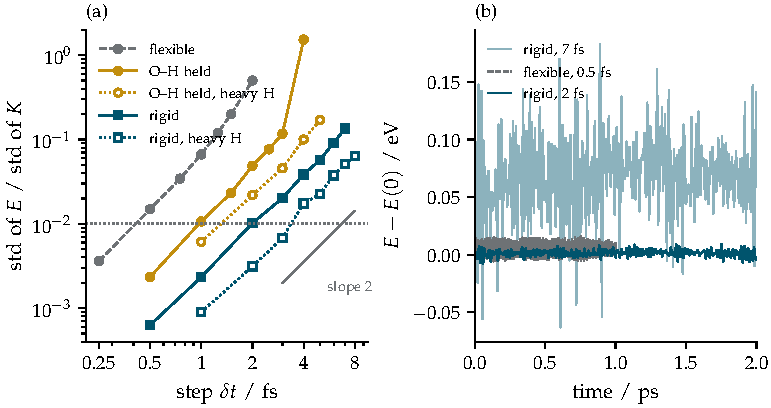
\includegraphics{ch11_constraints/step}
\caption{The step each model of water allows: 64 molecules, flexible (by
velocity Verlet), with the O--H bonds held, and rigid (both by RATTLE);
open markers for the last two with hydrogen made three times heavier
(\cref{sec:cs-mass}). (a) The standard deviation of the total energy over
that of the kinetic energy, against the step, over \SI{1}{\pico\second}
(flexible, O--H held) or \SI{2}{\pico\second} (rigid); dotted, the 1\%
level. (b) The total energy less its starting value for rigid water at 2
and \SI{7}{\femto\second} and flexible water at
\SI{0.5}{\femto\second}.}
\label{fig:cs-step}
\end{figure}

How small the ratio must be is a judgement, depending on what is to be
measured (\cref{sec:in-stability}). Taking 1\% as the level, and reading
where each curve crosses it between measured points, the flexible model
allows \SI{0.41}{\femto\second}, the model with its O--H bonds held
\SI{0.97}{\femto\second}, and the rigid model \SI{1.98}{\femto\second}:
holding the O--H bonds buys a factor of 2.4, and holding the angle too a
factor of 4.8. With the O--H bonds held, the fastest motion left is the
bend, with a period of \SI{17.0}{\femto\second} in this model, shorter
than the \SI{20.9}{\femto\second} of the free spring model, whose bonds
stretch as it bends; with all three distances held, the molecule cannot
vibrate at all, and the fastest motions left are the molecules' turning
back and forth in the cage of their neighbours. These steps are read from
single runs of 1 or \SI{2}{\pico\second}: the rigid run at
\SI{2}{\femto\second} gives 1.02\% over \SI{2}{\pico\second} and 0.93\%
over \SI{10}{\pico\second} (\cref{sec:cs-trajectory}), and since the
ratio grows as $\dt^2$ a difference of 10\% in it moves the step at 1\% by
about 5\%, a spread that Chapter~15 turns into an error bar. \Cref{fig:cs-step}(b) shows that even at
\SI{7}{\femto\second}, where the ratio is 13\%, the energy of rigid water
stays in a band over \SI{2}{\pico\second}, its mean moving by
\SI{0.007}{\electronvolt\per\pico\second}, as a symplectic method's
should; at \SI{2}{\femto\second} the band is \SI{0.017}{\electronvolt}
wide for the whole box, \SI{0.26}{\milli\electronvolt} per molecule.

The rigid model is a different model, however long its step. Water held
rigid cannot stretch or bend, and any property that depends on those
motions, such as its spectrum at high frequencies, is lost; the
properties of liquid water that depend on how molecules move as wholes
are what a rigid model is built to give. A rigid model is therefore a
choice of model as much as a means of lengthening the step, and the
planned comparisons with learned propagators in Part~VI use the flexible
model as the reference when those vibrations are retained.

\begin{practice}
The tolerance of the constraints matters. The step test above holds the
bonds to $10^{-10}$; a tolerance of $10^{-3}$ leaves errors of
\SI{1.5e-3}{\angstrom} and an energy that drifts
(\cref{sec:cs-trajectory}). A tolerance may be stated as a relative or an
absolute error of the length or of its square, so the numbers to check in
a run are the largest error of a held distance, which \texttt{mdlab}
records as \texttt{bond\_error}, and whether a tighter tolerance changes
the energy.
\end{practice}

\begin{keyidea}
Measured on 64 molecules of TIP3P water, at an energy fluctuation of 1\%
of the kinetic energy's, holding the O--H bonds lengthens the step from
0.41 to \SI{0.97}{\femto\second}, and holding all three distances to
\SI{1.98}{\femto\second}: factors of 2.4 and 4.8, bought by removing the
fastest vibrations, and with them the motions that depended on them.
\end{keyidea}

\notebook{11}{compare the three models' energy at any step}

\begin{selfcheck}
How many steps of \SI{0.41}{\femto\second} and of
\SI{1.98}{\femto\second} cover a nanosecond?
\end{selfcheck}

%=============================================================================!
% 11.4  MULTIPLE TIME STEPS                                                   !
%=============================================================================!
\section{Multiple time steps}
\label{sec:cs-respa}

Constraints remove the fast motions. A second route keeps every motion
and recognises that the forces behind them differ, in how fast they change
and in what they cost. In the flexible water of \cref{sec:cs-water}, the
springs inside each molecule change over the \SI{7.33}{\femto\second}
period of its fastest vibration and cost almost nothing to compute: one
call for all 64 molecules takes \SI{0.04}{\milli\second}. The
Lennard-Jones and Ewald forces between molecules change mainly as whole
molecules move and turn, and one call takes between 23 and
\SI{26}{\milli\second} in our measurements, some 600 times as long. Velocity Verlet
computes both at every step of \SI{0.41}{\femto\second}. This section
builds a method that computes the costly forces less often.

\subsection*{A splitting within a splitting}

\Cref{sec:in-splitting} split the Liouville operator into a part
$\Liou_{\mathrm r}$ that moves the positions and a part $\Liou_{\mathrm
p}$ that moves the momenta by the forces. The forces are a sum, fast plus
slow, $\vb{F}_i = \vb{F}_i^{\mathrm f} + \vb{F}_i^{\mathrm s}$, and since
$\Liou_{\mathrm p}A = \sum_i\vb{F}_i\cdot\grad_{\vb{p}_i}A$ contains each
force to the first power, it splits in the same way, $\Liou_{\mathrm p} =
\Liou_{\mathrm p}^{\mathrm f} + \Liou_{\mathrm p}^{\mathrm s}$, each part a
kick by its own forces alone. The derivation of \cref{eq:in-trotter}
used nothing about $X$ and $Y$ beyond keeping the order of their products,
so with $X = \Liou_{\mathrm p}^{\mathrm s}$ and $Y = \Liou_{\mathrm r} +
\Liou_{\mathrm p}^{\mathrm f}$ it gives
\begin{equation*}
   \mathrm{e}^{\dt\Liou} = \mathrm{e}^{\frac12\dt\Liou_{\mathrm p}^{\mathrm s}}
   \,\mathrm{e}^{\dt(\Liou_{\mathrm r} + \Liou_{\mathrm p}^{\mathrm f})}\,
   \mathrm{e}^{\frac12\dt\Liou_{\mathrm p}^{\mathrm s}} + \order{\dt^3} :
\end{equation*}
half a kick by the slow forces, the motion for $\dt$ under the fast forces
alone, and half a kick by the slow forces. The middle factor is the
motion of a system with only the cheap forces, which $n$ velocity Verlet
steps of $\dt/n$ follow,
\begin{equation*}
   \mathrm{e}^{\dt(\Liou_{\mathrm r} + \Liou_{\mathrm p}^{\mathrm f})}
   = \Bigl(\mathrm{e}^{\frac{\dt}{2n}\Liou_{\mathrm p}^{\mathrm f}}\,
   \mathrm{e}^{\frac{\dt}{n}\Liou_{\mathrm r}}\,
   \mathrm{e}^{\frac{\dt}{2n}\Liou_{\mathrm p}^{\mathrm f}}\Bigr)^n
   + \order{\dt^3/n^2} ,
\end{equation*}
the error of $n$ steps each in error by order $(\dt/n)^3$, $n(\dt/n)^3
= \dt^3/n^2$ in all. The outer
step is $\dt$, taken with one call of the slow forces; the inner step is
$\dt/n$, taken $n$ times with one call of the fast forces each. Every factor is a
kick or a drift, so the product, like velocity Verlet, keeps the full
symplectic condition (\cref{sec:in-reversal}), and since it reads the same
from either end, reversing the velocities and stepping again undoes it
factor by factor, as for velocity Verlet in \cref{sec:in-reversal}: it is
reversible. Tuckerman, Berne and Martyna derived the
method in this way, as the reversible reference system propagator
algorithm, RESPA\cite{Tuckerman1992}. With $n = 1$ it is velocity Verlet
with the two forces added (\cref{ex:cs-respa-one}).

The function \texttt{respa\_step} of \texttt{mdlab.respa} is the outer
step:
\begin{code}
    v += 0.5 * dt * force_to_accel * np.asarray(slow_forces) / m
    u_fast = 0.0
    for _ in range(n_inner):
        v += 0.5 * h * force_to_accel * f_fast / m
        r += h * v
        u_fast, f_fast = fast(r)
        v += 0.5 * h * force_to_accel * f_fast / m
    u_slow, f_slow = slow(r)
    v += 0.5 * dt * force_to_accel * f_slow / m
\end{code}
\noindent where \texttt{h} is the inner step $\dt/n$ and \texttt{f\_fast}
holds the fast forces at the start of the step, passed in from the step
before. Its test checks
that with one inner step it gives the
positions and velocities of velocity Verlet to $10^{-12}$. For water,
\texttt{WaterModel} supplies the two parts: \texttt{intramolecular}, the
springs, as the fast forces, and \texttt{intermolecular}, Lennard-Jones
and Ewald, as the slow ones.

\subsection*{What it buys}

\Cref{fig:cs-respa} runs the flexible box with inner steps of
\SI{0.25}{\femto\second}, at which velocity Verlet alone keeps the energy
fluctuation at 0.36\% of the kinetic energy's, and outer steps from
\SI{0.25}{\femto\second} to \SI{4.5}{\femto\second}. At an outer step of
\SI{1}{\femto\second} the fluctuation is 1.8\%, where velocity Verlet at
the same step gives 6.7\%. At the 1\% level RESPA reaches an outer step
of \SI{0.72}{\femto\second} against velocity Verlet's
\SI{0.41}{\femto\second}, 1380 calls of the slow forces per picosecond
against 2430 (from the steps before rounding), a factor of 1.76; at 2\% the factor is 1.82
(\cref{fig:cs-respa}b). Since the slow forces take nearly all the time,
the run is faster by close to that factor.

\begin{figure}[htb]
\centering
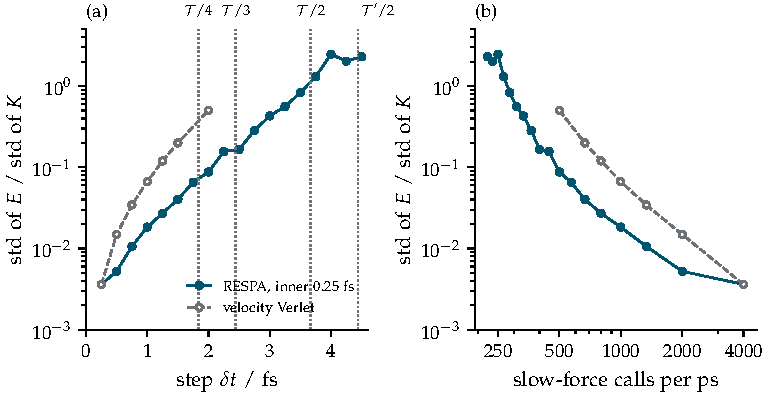
\includegraphics{ch11_constraints/respa}
\caption{Multiple time steps for 64 molecules of flexible water: the
springs are the fast forces, followed with inner steps of
\SI{0.25}{\femto\second}; Lennard-Jones and Ewald forces are the slow
ones, applied once per outer step $\dt$. (a) The standard deviation of the
total energy over that of the kinetic energy, against $\dt$, for RESPA
and for velocity Verlet taking all forces at every step $\dt$ (dashed);
dotted, a quarter, a third and a half of the period $\mathcal{T} =
\SI{7.33}{\femto\second}$ of the fastest vibration, and half the next,
$\mathcal{T}' = \SI{8.88}{\femto\second}$. (b) The same fluctuation
against the number of calls of the slow forces per picosecond, which sets
the cost of a run.}
\label{fig:cs-respa}
\end{figure}

The gain stops early. Beyond an outer step of about
\SI{1.8}{\femto\second}, a quarter of the fastest period, the fluctuation
climbs much faster than $\dt^2$, to 8.8\% at \SI{2}{\femto\second} and
43\% at \SI{3}{\femto\second}, and the run blows up at
\SI{4.5}{\femto\second}. Following the fast motion more closely does not
help: inner steps of \SI{0.125}{\femto\second} with an outer step of
\SI{2}{\femto\second} give 10.4\%, no better than 8.8\%. What fails is
the outer step itself, and \cref{sec:cs-resonance} finds why.

\begin{keyidea}
RESPA splits the forces into fast and slow parts and the Liouville
operator with them: half a kick by the slow forces, $n$ velocity Verlet
steps of $\dt/n$ under the fast forces alone, and half a kick by the slow
forces. It is reversible and symplectic. On flexible water it cuts the
calls of the costly forces by a factor of about 1.8 at equal accuracy, and
fails beyond outer steps of about a quarter of the fastest period.
\end{keyidea}

\notebook{11}{split the forces of water and choose the outer step}

\begin{selfcheck}
With \SI{24}{\milli\second} and \SI{0.04}{\milli\second} per call, about how long does one picosecond of
flexible water take by velocity Verlet at \SI{0.41}{\femto\second}, and by
RESPA at an outer step of \SI{0.72}{\femto\second} with three inner
steps?
\end{selfcheck}

%=============================================================================!
% 11.5  RESONANCE                                                             !
%=============================================================================!
\section{Resonance}
\label{sec:cs-resonance}

RESPA applies the slow forces as sudden kicks, once per outer step, to
atoms that are vibrating under the fast forces in between. A swing pushed
in step with its motion goes higher, and without drag higher and higher
(\cref{sec:os-driven}); kicks that come in step with a vibration, once in
every half swing or every swing, can pump it in the same way. This section
finds the outer steps at which that happens for the simplest system that
shows it, and compares the result with water.

\subsection*{Two springs}

One coordinate $q$, of unit mass, is pulled back by a fast spring and a
slow one, with angular frequencies $\omega_{\mathrm f}$ and
$\omega_{\mathrm s}$, so its force is $-(\omega_{\mathrm f}^2 +
\omega_{\mathrm s}^2)\,q$. RESPA follows the fast spring with many inner
steps, closely enough to take its motion as exact: by the solution of
\cref{sec:ne-spring}, over a time $\dt$ it carries the state $(q, v)$ to
\begin{equation*}
   q' = q\cos\theta + \frac{v}{\omega_{\mathrm f}}\sin\theta , \qquad
   v' = -\omega_{\mathrm f}q\sin\theta + v\cos\theta , \qquad
   \theta = \omega_{\mathrm f}\dt ,
\end{equation*}
and half a kick by the slow spring changes $v$ by $-\frac12\dt\,
\omega_{\mathrm s}^2q$ and leaves $q$. Both are linear, so as matrices
acting on the column $(q, v)$,
\begin{equation*}
   \vb{R} = \begin{pmatrix} \cos\theta & \sin\theta/\omega_{\mathrm f}\\
   -\omega_{\mathrm f}\sin\theta & \cos\theta \end{pmatrix} , \qquad
   \vb{K} = \begin{pmatrix} 1 & 0\\ -\kappa & 1 \end{pmatrix} , \qquad
   \kappa = \tfrac12\dt\,\omega_{\mathrm s}^2 ,
\end{equation*}
and the outer step is $\vb{M} = \vb{K}\vb{R}\vb{K}$, the half kick
$\vb{K}$ acting first. Multiplying, with $C = \cos\theta$ and $S =
\sin\theta$,
\begin{align*}
   \vb{R}\vb{K} &= \begin{pmatrix} C - \kappa S/\omega_{\mathrm f} &
      S/\omega_{\mathrm f}\\ -\omega_{\mathrm f}S - \kappa C & C
      \end{pmatrix} ,\\
   \vb{K}\vb{R}\vb{K} &= \begin{pmatrix} C - \kappa S/\omega_{\mathrm f} &
      S/\omega_{\mathrm f}\\ -\omega_{\mathrm f}S - 2\kappa C
      + \kappa^2S/\omega_{\mathrm f} & C - \kappa S/\omega_{\mathrm f}
      \end{pmatrix} ,
\end{align*}
so the trace, the sum of the diagonal entries (\cref{sec:in-reversal}),
is $2C - 2\kappa S/\omega_{\mathrm f}$, which with $2\kappa = \dt\,
\omega_{\mathrm s}^2$ is
\begin{equation}
   \operatorname{tr}\vb{M} = 2\cos\theta
   - \frac{\omega_{\mathrm s}^2\dt}{\omega_{\mathrm f}}\sin\theta .
   \label{eq:cs-trace}
\end{equation}
The fast motion $\vb{R}$, which turns the point $(q, v/\omega_{\mathrm f})$
through the angle $\theta$, and the kick $\vb{K}$ each keep area in the
phase plane (determinants $\cos^2\theta + \sin^2\theta = 1$ and $1$), so
their product does too, and $\det\vb{M} = 1$ (\cref{sec:ha-symplectic}).
Whether repeated outer steps stay bounded depends on the trace alone.

\begin{toolbox}[Powers of a $2\times2$ matrix]
Any $2\times2$ matrix $\vb{M}$, with $M_{11}$, $M_{12}$ in its first row
and $M_{21}$, $M_{22}$ in its second, satisfies
\begin{equation*}
   \vb{M}^2 = (\operatorname{tr}\vb{M})\,\vb{M} - (\det\vb{M})\,\vb{I} ,
\end{equation*}
as multiplying out shows: $\vb{M}^2$ has $M_{11}^2 + M_{12}M_{21}$ and
$M_{11}M_{12} + M_{12}M_{22}$ in its first row and $M_{21}M_{11} +
M_{22}M_{21}$ and $M_{21}M_{12} + M_{22}^2$ in its second, while $(M_{11}
+ M_{22})\vb{M}$ has $M_{11}^2 + M_{11}M_{22}$, $M_{11}M_{12} +
M_{12}M_{22}$ and $M_{21}M_{11} + M_{21}M_{22}$, $M_{11}M_{22} +
M_{22}^2$, and subtracting $(M_{11}M_{22} - M_{12}M_{21})\vb{I}$ from the
latter gives the former. With $\det\vb{M} = 1$, multiplying by
$\vb{M}^{n-1}$ gives $\vb{M}^{n+1} = (\operatorname{tr}\vb{M})\vb{M}^n -
\vb{M}^{n-1}$, so each entry $x_n$ of the state after $n$ steps,
$\vb{M}^n$ times the start, obeys
\begin{equation*}
   x_{n+1} = (\operatorname{tr}\vb{M})\,x_n - x_{n-1} .
\end{equation*}
This is the recurrence of \cref{sec:in-shadow}. If
$\lvert\operatorname{tr}\vb{M}\rvert < 2$, then $\operatorname{tr}\vb{M} =
2\cos\phi$ for some angle $\phi$, and $\cos n\phi$ and $\sin n\phi$ solve
it, as shown there: the motion stays bounded. If
$\lvert\operatorname{tr}\vb{M}\rvert > 2$, the quadratic $\Lambda^2 -
(\operatorname{tr}\vb{M})\Lambda + 1 = 0$ has, by the quadratic formula, a
real root $\Lambda$ with $\lvert\Lambda\rvert > 1$, and dividing it by
$\Lambda$ gives $\Lambda + 1/\Lambda = \operatorname{tr}\vb{M}$. Then
$\Lambda^{n+1} = (\Lambda + 1/\Lambda)\Lambda^n - \Lambda^{n-1}$, so $x_n =
\Lambda^n$ solves the recurrence, as does $\Lambda^{-n}$, and a general
start, a mixture of the two, grows by the factor $\lvert\Lambda\rvert$ at
every step. At $\lvert\operatorname{tr}\vb{M}\rvert = 2$ exactly the growth,
if any, is slower, by a fixed amount at each step.
\end{toolbox}

Without the slow spring, $\operatorname{tr}\vb{M} = 2\cos\theta$, which
never leaves $[-2, 2]$: exact inner motion is stable at any outer step.
The slow spring adds $-b\theta\sin\theta$ to the trace, with $b =
(\omega_{\mathrm s}/\omega_{\mathrm f})^2$, since $\omega_{\mathrm s}^2
\dt/\omega_{\mathrm f} = b\,\omega_{\mathrm f}\dt$. Just below
$\theta = \pi$ we write $\theta = \pi - \epsilon$ with $\epsilon$ small and
positive; then $\cos\theta = -\cos\epsilon \approx -1 + \frac12\epsilon^2$
and $\sin\theta = \sin\epsilon \approx \epsilon$ (\cref{sec:mo-taylor}),
and
\begin{align*}
   \tfrac12\operatorname{tr}\vb{M} &\approx -1 + \tfrac12\epsilon^2
   - \tfrac12b\pi\epsilon && \text{with $\theta \approx \pi$ in the last
   term,}\\
   &< -1 \quad\text{when}\quad \tfrac12\epsilon^2 < \tfrac12b\pi\epsilon ,
   \text{ that is, } 0 < \epsilon < b\pi .
\end{align*}
The motion therefore grows for outer steps in a band just below $\theta =
\pi$, half the fast period $\mathcal{T}_{\mathrm f} = 2\pi/\omega_{\mathrm
f}$, of width $b\pi$ in $\theta$, or $\frac12b\,\mathcal{T}_{\mathrm f}$
in $\dt$; just below $\theta = 2\pi$, where $\sin\theta$ is negative, the
same argument gives a band twice as wide below $\mathcal{T}_{\mathrm f}$
(\cref{ex:cs-band}). Near $\dt = \frac12\mathcal{T}_{\mathrm f}$ the kicks
come every half vibration, when the fast motion has carried $q$ to minus
its value, and each one, proportional to $q$, meets the vibration in the
same phase as the last: a resonance. Together the two springs shorten the
period to $\mathcal{T}_{\mathrm f}/\sqrt{1 + b}$, so the band lies just
below $\frac12\mathcal{T}_{\mathrm f}$, around half that period. At
$\dt = \frac12\mathcal{T}_{\mathrm f}$ exactly, $\theta = \pi$, the trace
is $-2$, and $\vb{M}$ has rows $(-1, 0)$ and $(2\kappa, -1)$: $q$ comes
back to minus itself at every step while $v$ gains $2\kappa q$ each time,
so the motion grows steadily rather than by a factor.

\Cref{fig:cs-resonance} measures it for $\omega_{\mathrm s} =
0.3\,\omega_{\mathrm f}$, so $b = 0.09$ and the predicted width below
$\frac12\mathcal{T}_{\mathrm f}$ is $0.045\,\mathcal{T}_{\mathrm f}$. The
trace of \cref{eq:cs-trace} leaves $[-2, 2]$ for $\dt$ from 0.459 to
$0.500\,\mathcal{T}_{\mathrm f}$, a width of 0.041, since the term
$\frac12b\epsilon^2$ dropped with $\theta \approx \pi$ narrows the band by
the factor $1/(1 + b)$, and from 0.919 to $1.000\,\mathcal{T}_{\mathrm
f}$. RESPA run for 300 steps from $q = 1$ at rest reaches a size
$\sqrt{q^2 + (v/\omega_{\mathrm f})^2}$ of $\num{2.9e17}$ at
$0.48\,\mathcal{T}_{\mathrm f}$, grows steadily to 23 at
$0.50\,\mathcal{T}_{\mathrm f}$, and stays near its start, below 2, at
0.45 and $0.52\,\mathcal{T}_{\mathrm f}$.

\begin{figure}[htb]
\centering
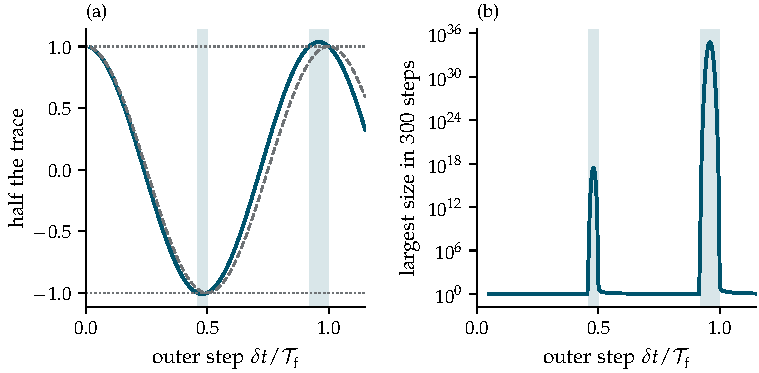
\includegraphics{ch11_constraints/resonance}
\caption{Resonance of a fast spring kicked by a slow one, $\omega_{\mathrm
s} = 0.3\,\omega_{\mathrm f}$, stepped by RESPA with 50 inner steps.
(a) Half the trace of the outer step, \cref{eq:cs-trace}, against the
outer step in units of the fast period; the motion grows where it passes
$\pm1$ (dotted), in the shaded bands, and the dashed curve, $\cos\theta$,
is half the trace without the slow spring. (b) The largest size of the
state, $\sqrt{q^2 + (v/\omega_{\mathrm f})^2}$, in 300 outer steps from $q
= 1$ at rest.}
\label{fig:cs-resonance}
\end{figure}

\subsection*{In water}

Water has many fast vibrations, and its slow forces are not springs, but
the same picture explains part of \cref{fig:cs-respa}. The energy drifts
most for outer steps around half the periods of the model's two
stretches, 3.67 and \SI{4.44}{\femto\second}: by $+0.19$, $+1.14$,
$+2.25$ and \SI{+0.33}{\electronvolt\per\pico\second} at 3.5, 3.75, 4 and
\SI{4.25}{\femto\second}, and the run blows up at
\SI{4.5}{\femto\second}. The fluctuation grows too fast well before those
steps. From an outer step of 1 to \SI{2}{\femto\second} it grows by a
factor of 4.8, a little more than the factor of 4 of $\dt^2$, and from 2
to \SI{3}{\femto\second} by 4.9, against 2.25. Ma, Izaguirre and Skeel
found the same in flexible water and proteins, and traced it to
resonances of a kind that the linear model above lacks, with
instabilities when the outer step is a third or possibly a quarter of the
fastest period\cite{Ma2003}: here 2.44 and \SI{1.83}{\femto\second}. The
outer step of RESPA is therefore kept below a third of the fastest
period, and for this water a quarter, whatever the cost of the slow
forces.

\begin{keyidea}
Kicks by the slow forces once per outer step can pump a fast vibration.
For two springs the outer step's matrix has the trace $2\cos\theta -
(\omega_{\mathrm s}^2\dt/\omega_{\mathrm f})\sin\theta$, and the motion
grows where it leaves $[-2, 2]$, in bands just below multiples of half
the fast period. In water the fluctuation climbs faster than $\dt^2$
beyond about a quarter of the fastest period, where Ma, Izaguirre and
Skeel found resonances beyond this linear picture.
\end{keyidea}

\notebook{11}{move the outer step across the resonance bands}

\begin{selfcheck}
For $\omega_{\mathrm s} = 0.1\,\omega_{\mathrm f}$ and a fast period of
\SI{9}{\femto\second}, where is the band of growth below half the period,
and how wide is it?
\end{selfcheck}

%=============================================================================!
% 11.6  HEAVIER HYDROGENS                                                     !
%=============================================================================!
\section{Heavier hydrogens}
\label{sec:cs-mass}

The potential energy depends only on where the atoms are; the masses
enter only through Newton's law, and set how fast the
atoms respond to the forces. A third way to lengthen the step changes the
masses so that the fastest motions slow down, while keeping the energy
surface, and with it the forces, as it was. This section works out what
the change does to the vibrations of water and measures the step it buys.

\subsection*{Moving mass}

A bond between two atoms vibrates with $\omega = \sqrt{k/m_{\mathrm r}}$
(\cref{sec:os-bodies}), and for a bond to hydrogen the reduced mass is
close to the hydrogen's own: for O--H, $m_{\mathrm r} = 15.999\times1.008/
(15.999 + 1.008) = \SI{0.9483}{\amu}$. Hydrogen mass repartitioning makes
each hydrogen heavier and takes the same mass from the atom it is bonded
to, so that every molecule keeps its total mass. Tripling the hydrogen's
mass to \SI{3.024}{\amu} takes $2\times2.016$ from the oxygen of water,
leaving \SI{11.967}{\amu}; the molecule still weighs \SI{18.015}{\amu}, so
its centre of mass, now a little nearer the hydrogens
(\cref{ex:cs-hmr-centre}), has the same acceleration, the total force
over the total mass, as before. The O--H reduced mass becomes
$11.967\times3.024/(11.967 + 3.024) = \SI{2.4140}{\amu}$, 2.55 times
larger, and the stretch slows by $\sqrt{2.55} = 1.60$. The function
\texttt{repartition\_masses} of \texttt{mdlab.constraints} makes the
change for any list of bonds to hydrogen.

The normal modes of the spring model of water (\cref{sec:ro-freedom})
with the new masses show a similar slowing, by 1.68 for the fastest
vibration, which falls from
$\omega = 0.857$ to \SI{0.509}{\radian\per\femto\second}, its period rises
from 7.33 to \SI{12.35}{\femto\second}, and the stability limit $2/\omega$
of \cref{sec:in-stability} from 2.33 to \SI{3.93}{\femto\second}; the bend
slows from a period of 20.9 to \SI{32.2}{\femto\second}, and with the O--H
bonds held from 17.0 to \SI{27.2}{\femto\second}. A rigid molecule
cannot vibrate, but it turns, and moving mass outwards from the oxygen to
the hydrogens raises its moments of inertia (\cref{sec:ro-tensor}): the
principal moments, at the TIP3P shape, go from 0.615, 1.155 and \SI{1.770}{\amu\,\angstrom
\squared} to 1.379, 3.465 and \SI{4.844}{\amu\,\angstrom\squared}, so its
turning in the cage of its neighbours slows too.

\subsection*{What it buys}

The open markers of \cref{fig:cs-step}(a) measure it on the box of 64
molecules. At the 1\% level, water with its O--H bonds held goes from
0.97 to \SI{1.31}{\femto\second} with heavier hydrogens, a factor of
1.35, although its bend, the fastest motion left, slows by 1.60, so the
bend is not all that sets its step; rigid water goes from 1.98 to
\SI{3.38}{\femto\second}, a factor of 1.71, and is then 8.2 times the
step of the flexible model with ordinary masses. Hopkins and co-workers,
citing earlier studies in which repartitioning let the step be increased
by up to a factor of two, ran a short chain of three amino acids and a
protein with repartitioned masses and steps of
\SI{4}{\femto\second}\cite{Hopkins2015}.

\subsection*{What it keeps, and what it changes}

Repartitioning leaves the potential energy and the forces unchanged, and
Chapter~12 shows that the probability of finding the atoms in a given
arrangement, at a given temperature, depends on the potential energy
alone and not on the masses. Averages over the arrangements of the atoms,
such as their mean potential energy or how the molecules are packed, are
therefore unchanged, exactly so for molecules that are free or held wholly
rigid; with only some distances held, as with the O--H bonds alone, the
held distances make the masses enter the probability of the angles left
free, a small effect that this book does not pursue. Everything that depends on how fast the atoms move is
changed: heavier hydrogens move more slowly, so the rates at which
molecules turn and diffuse, and the frequencies of their vibrations,
belong to a system with different masses. Hopkins and co-workers report no
significant difference in the rates and the equilibrium properties they
computed with \SI{4}{\femto\second} steps and repartitioned
masses\cite{Hopkins2015};
that is a finding about their systems and properties, and a study of
motion at the atomic scale should check its own.

\begin{keyidea}
Moving mass from heavy atoms to their hydrogens keeps the total mass and
the forces, and raises the reduced masses of the fastest bonds: tripling
hydrogen's mass in water slows the O--H stretch by a factor of 1.60. On
64 molecules it lengthens the step at 1\% by 1.35 with only the O--H bonds
held and by 1.71 for rigid water. Averages over arrangements are kept,
exactly for free or rigid molecules; rates of motion are not.
\end{keyidea}

\notebook{11}{choose the hydrogen mass and watch the vibrations slow}

\begin{selfcheck}
In a C--H bond, carbon \SI{12.011}{\amu} and hydrogen \SI{1.008}{\amu}, the
hydrogen is made three times heavier at the carbon's expense. By what
factor does the stretch slow?
\end{selfcheck}

%=============================================================================!
% 11.7  HOW FAR THESE METHODS GO                                              !
%=============================================================================!
\section{How far these methods go}
\label{sec:cs-limits}

\Cref{tab:cs-steps} collects the steps measured in this chapter on the
same 64 molecules of water, each at the energy fluctuation of 1\% of the
kinetic energy's that \cref{sec:cs-water} took as the level. The cost of
a run is set by the calls of the costly forces between molecules, one per
step, or per outer step for RESPA.

\begin{table}[htb]
\centering
\caption{The step at which the energy fluctuation of 64 water molecules
reaches 1\% of the kinetic energy's, with each method of this chapter;
the gain over flexible water by velocity Verlet; and the calls of the
forces between molecules per picosecond, from the unrounded steps. Heavy H: hydrogen three times as
heavy, at the oxygen's expense.}
\label{tab:cs-steps}
\begin{tabular}{llccc}
\toprule
model and method & fastest motion left & step / fs & gain & calls per ps\\
\midrule
flexible, velocity Verlet & O--H stretch & 0.41 & 1 & 2430\\
flexible, RESPA & O--H stretch & 0.72 & 1.8 & 1380\\
O--H held & bend & 0.97 & 2.4 & 1030\\
O--H held, heavy H & bend, slower & 1.31 & 3.2 & 765\\
rigid & turning & 1.98 & 4.8 & 505\\
rigid, heavy H & turning, slower & 3.38 & 8.2 & 296\\
\bottomrule
\end{tabular}
\end{table}

Each method removes the fastest motion or slows it, and the next fastest
then sets the step. Holding the O--H bonds leaves the bend; holding the
angle too leaves the turning of whole molecules; heavier hydrogens slow
whatever is left. RESPA keeps every motion; at the 1\% level its outer
step is \SI{0.72}{\femto\second}, and resonance holds it below about a
quarter of the fastest period, \SI{1.8}{\femto\second}, whatever level is
accepted (\cref{sec:cs-resonance}). The factors are of a few each, and they
combine: rigid water with heavier hydrogens takes steps 8.2 times as long
as the flexible model, but it is no longer the same model. For a
simulation that keeps every motion, the gain here is the 1.8 of RESPA.

A factor of thirty, which TrajCast reaches on quartz, would need steps of
\SI{12}{\femto\second} for the flexible model, longer than the period of its fastest vibration,
\SI{7.33}{\femto\second}. Such steps lie outside the range of the methods developed here.
Velocity Verlet becomes unstable beyond $2/\omega$
(\cref{sec:in-stability}), \SI{2.33}{\femto\second} here, and every
method of this chapter must still follow, with steps short compared with
its period, the fastest motion it keeps. The authors of TrajCast make the
same point about methods with multiple time steps, which are
`fundamentally limited by the need for small time steps in parts of the
system'\cite{Thiemann2026}. TrajCast itself, run on 64 molecules of
flexible water in a box of nearly the same size as this chapter's, though
with a different model of water, takes strides of $\Dt =
\SI{5}{\femto\second}$, ten times the \SI{0.5}{\femto\second} step of the
simulations it learned from, and on quartz strides of
\SI{30}{\femto\second}, thirty times the \SI{1}{\femto\second} step of its
simulations\cite{Thiemann2026}. A stride of \SI{5}{\femto\second} already
exceeds the stability limit of velocity Verlet for the faster O--H stretch
of real water, of period \SI{8.88}{\femto\second}, which is
\SI{2.83}{\femto\second} (\cref{sec:in-stability}), as well as the
\SI{2.33}{\femto\second} of this chapter's model. A learned map that predicts
the state a whole stride ahead is not bound by that limit, because it does
not step through the vibrations in between; what it must get right
instead, and how it can be trusted, is the subject of the planned Part~VI.

\begin{keyidea}
Constraints, heavier hydrogens and multiple time steps each lengthen the
step by a factor of a few, by removing or slowing the fastest motion,
until the next fastest sets the limit. For velocity Verlet, stability requires a step below $2/\omega$ for the
fastest vibration retained; this is a limit of that integrator, not of
every possible numerical method. A learned propagator is not bound by
the same limit, but its accuracy and sampled distribution still need
independent tests.
\end{keyidea}

\begin{selfcheck}
From \cref{tab:cs-steps}, how many calls of the forces between molecules
does a nanosecond of rigid water with heavier hydrogens take, and how
many does flexible water by velocity Verlet take?
\end{selfcheck}

%=============================================================================!
% 11.8  WHAT THE TRAJECTORY LOOKS LIKE                                        !
%=============================================================================!
\section{What the trajectory looks like}
\label{sec:cs-trajectory}

A run produces a record: energies at every step, positions and
velocities every so often. Before any of it is used, the record should be
read for signs that the run went wrong, and many faults show in it
clearly when the reader knows where to look. This section shows a
healthy run of rigid water and the same run broken in eight ways, each
caught by a check of \texttt{mdlab.diagnostics} or of the record itself. Later chapters add the
checks of temperature, pressure and thermostats, and Chapter~17 collects
them all.

\subsection*{A healthy run}

\Cref{fig:cs-healthy} follows the 64 rigid molecules for
\SI{10}{\pico\second}, 5000 steps of \SI{2}{\femto\second} by RATTLE. The
kinetic and potential energies swing by up to about
\SI{13}{\milli\electronvolt} per molecule over the first
\SI{2}{\pico\second}, in opposite directions, so that their sum, the total
energy, stays in a band \SI{0.31}{\milli\electronvolt} wide per molecule
over the whole run, \SI{0.020}{\electronvolt} for the box: the mirror image
of $K$ and $U$ is the first sign of a healthy run without a thermostat.
The standard deviation of the total energy is 0.93\% of the kinetic
energy's, just inside the 1\% level chosen in \cref{sec:cs-water}. The
mean total energy over the second half of the run, less that over the
first, is \SI{1.1e-5}{\electronvolt}, and divided by the
\SI{5}{\pico\second} between the centres of the halves it gives a drift of
\SI{2.2e-6}{\electronvolt\per\pico\second}, far below the fluctuation;
this is what \texttt{energy\_drift} computes. Every held distance stays
within \SI{1.5e-10}{\angstrom} of its length, the tolerance of $10^{-10}$
times the H--H length, and the centre of mass moves
\SI{1.8e-10}{\angstrom} in \SI{10}{\pico\second}, the rounding of the
arithmetic. The root-mean-square displacement of the oxygen atoms, the
square root of the mean over them of the squared distance each has moved
from its start, grows steadily, \num{1.41}, 4.14 and
\SI{5.76}{\angstrom} after 1, 5 and \SI{10}{\pico\second}, the wandering
of molecules in a liquid that Chapter~16 turns into a diffusion
coefficient. Over the run the kinetic energy averages
\SI{4.99}{\electronvolt}, \SI{13.10}{\milli\electronvolt} per freedom,
with a standard deviation of \SI{0.29}{\electronvolt}; the potential
energy averages \SI{-0.403}{\electronvolt} per molecule. These are
averages over one run of \SI{10}{\pico\second}, given with their spread;
how far such averages can be trusted, their error bars, is the subject of
Chapter~15. \Cref{fig:cs-frames} shows three
frames, with three molecules marked to follow them.

\begin{figure}[htb]
\centering
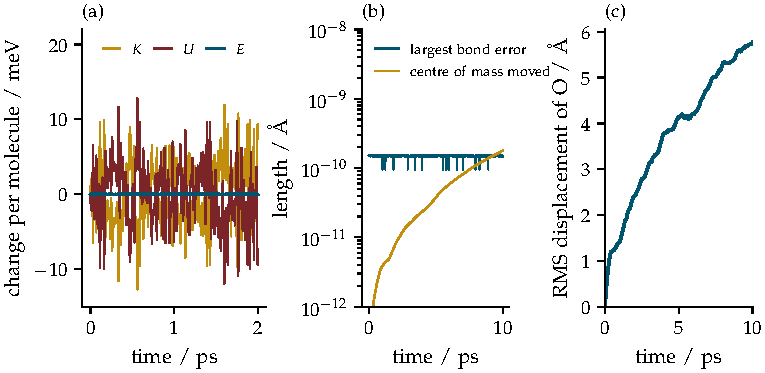
\includegraphics{ch11_constraints/healthy}
\caption{A healthy run: 64 rigid water molecules followed by RATTLE for
\SI{10}{\pico\second} with $\dt = \SI{2}{\femto\second}$. (a) The changes
of the kinetic, potential and total energies from their starting values,
per molecule, over the first \SI{2}{\pico\second}. (b) The largest error
of a held distance and the distance the centre of mass has moved, on a
logarithmic axis. (c) The root-mean-square distance the oxygen atoms have
moved from their starts.}
\label{fig:cs-healthy}
\end{figure}

\begin{figure}[htb]
\centering
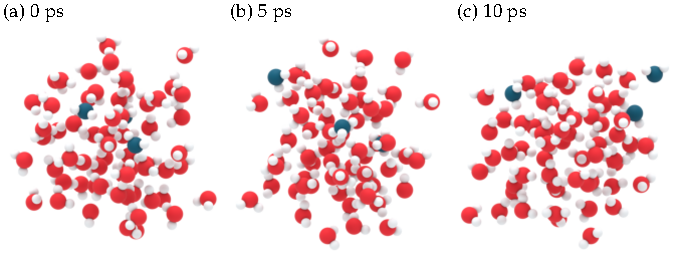
\includegraphics{ch11_constraints/frames}
\caption{Frames of the healthy run at 0, 5 and \SI{10}{\pico\second},
each molecule moved whole into the cell by its oxygen and drawn with its
two O--H bonds (oxygen red, hydrogen white). Three molecules have their
oxygen drawn in teal so that their motion can be followed. All frames are
seen from the same direction at the same scale.}
\label{fig:cs-frames}
\end{figure}

\subsection*{The same run, broken}

\Cref{fig:cs-faults} breaks the run in eight ways, each a mistake that is
easy to make, and \cref{tab:cs-faults} lists the check that catches each,
with its value in the healthy and the broken run.

\begin{figure}[p]
\centering
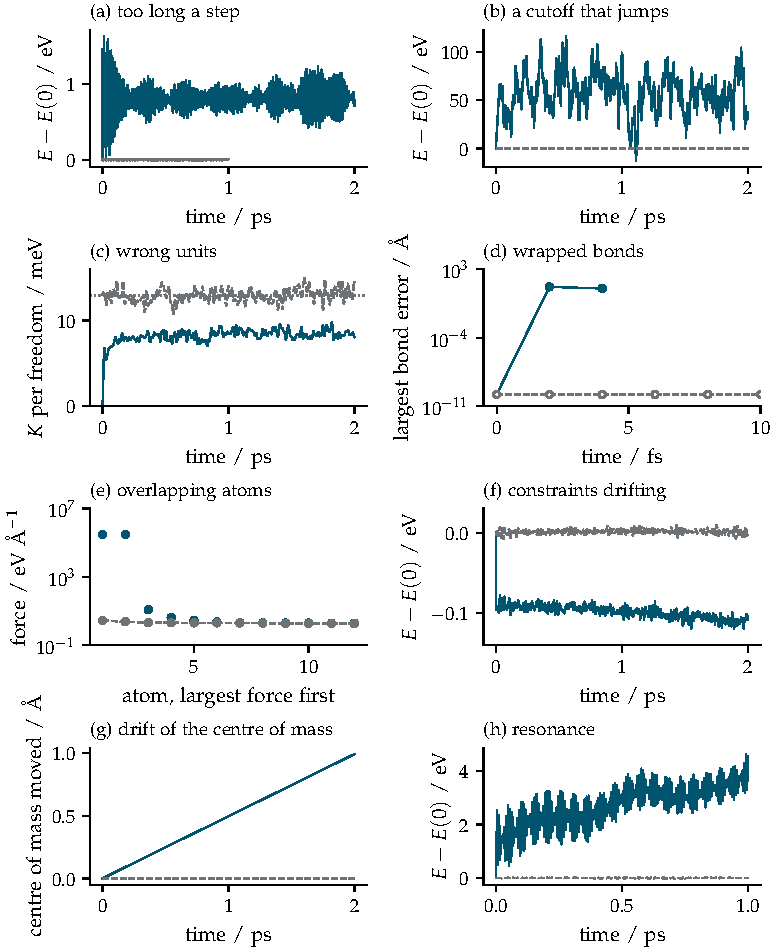
\includegraphics{ch11_constraints/faults}
\caption{The run of \cref{fig:cs-healthy} broken in eight ways (teal),
beside the healthy run (grey dashed), each through the quantity that
catches the fault. (a) Flexible water at \SI{2}{\femto\second} against
\SI{0.5}{\femto\second}. (b) The Coulomb energy cut off atom by atom at
\SI{6}{\angstrom} against the Ewald sum. (c) Velocities in
\si{\angstrom\per\femto\second} read as \aa ngstr\"oms per ASE time unit:
the kinetic energy per freedom against the value asked for (dotted).
(d) Positions wrapped into the cell at every step while the bonds are
measured without their nearest copies: the largest bond error. (e) One
molecule placed with its oxygen \SI{1}{\angstrom} from another's: the
forces at the start, largest first. (f) Constraints held to $10^{-3}$
against $10^{-10}$. (g) Starting velocities with their total momentum
left in. (h) RESPA with outer steps of \SI{4}{\femto\second} against
\SI{1}{\femto\second}.}
\label{fig:cs-faults}
\end{figure}

\begin{table}[htb]
\centering
\caption{The faults of \cref{fig:cs-faults}, the check of
\texttt{mdlab.diagnostics} or of the record that catches each, and its
value in the healthy run and in the broken one; runs of
\SI{2}{\pico\second}, except the flexible run at \SI{0.5}{\femto\second}
and both RESPA runs, of \SI{1}{\pico\second}, and runs that failed
sooner.}
\label{tab:cs-faults}
\small
\begin{tabular}{@{}llll@{}}
\toprule
fault & check & healthy & broken\\
\midrule
(a) step too long & \texttt{energy\_fluctuation} & 1.5\% & 47\%\\
(b) jumping cutoff & \texttt{energy\_fluctuation} & 1.0\% & 2100\%\\
(c) wrong units & $K(0)$ per freedom &
   \SI{12.9}{\milli\electronvolt} & \SI{0.125}{\milli\electronvolt}\\
(d) wrapped wrongly & \texttt{bond\_error} &
   \SI{1.5e-10}{\angstrom} & \SI{15.8}{\angstrom}\\
(e) overlap & \texttt{largest\_force} &
   \SI{2.9}{\electronvolt\per\angstrom} &
   \SI{3.0e5}{\electronvolt\per\angstrom}\\
(f) loose constraints & \texttt{energy\_drift} &
   \SI{4e-4}{\electronvolt\per\pico\second} &
   \SI{-0.011}{\electronvolt\per\pico\second}\\
(g) drift kept & \texttt{centre\_of\_mass\_path} &
   \SI{8e-12}{\angstrom} & \SI{0.99}{\angstrom}\\
(h) resonance & \texttt{energy\_drift} &
   \SI{2e-4}{\electronvolt\per\pico\second} &
   \SI{2.2}{\electronvolt\per\pico\second}\\
\bottomrule
\end{tabular}
\end{table}

\emph{(a) Too long a step.} Flexible water run at \SI{2}{\femto\second},
the step that suits rigid water, has an energy band 47\% of the kinetic
energy's spread, against 1.5\% at \SI{0.5}{\femto\second}, and a mean that
moves by \SI{0.016}{\electronvolt\per\pico\second}. The check is the
energy fluctuation, and the step test of \cref{sec:in-stability} confirms
the cause: halving the step should cut the fluctuation by about four, but
from 2 to \SI{1}{\femto\second} it cuts it by 7.5, so
\SI{2}{\femto\second} lies beyond the range where it grows as $\dt^2$.

\emph{(b) A cutoff that jumps.} Replacing the Ewald sum by the Coulomb
energy of pairs closer than \SI{6}{\angstrom}, cut off atom by atom, makes
the energy jump whenever a pair crosses the cutoff: an oxygen and a
hydrogen of different molecules have
$k_{\mathrm e}q_{\mathrm O}q_{\mathrm H}/r = \SI{-0.835}{\electronvolt}$
there. The total energy leaps by \SI{48}{\electronvolt} in the first
\SI{18}{\femto\second} and then wanders over some \SI{130}{\electronvolt},
its standard deviation 21 times the kinetic energy's, while its mean moves
by \SI{-8.2}{\electronvolt\per\pico\second}: the fault of
\cref{sec:pe-cutoffs} at its worst. A band or a drift that does not shrink
as the step is shortened points to forces that are not the slopes of a
smooth energy.

\emph{(c) Wrong units.} ASE measures time in its own unit,
\aa ngstr\"oms times $\sqrt{\mathrm{amu}/\mathrm{eV}}$, which is
$1/\sqrt{\texttt{FORCE\_TO\_ACCEL}} = \SI{10.18}{\femto\second}$ with the
factor of \cref{sec:ne-atoms}. Velocities written in
\si{\angstrom\per\femto\second} and read by a program that takes them in
that unit are 10.18 times too small, and the kinetic energy $10.18^2 =
104$ times too small: \SI{0.125}{\milli\electronvolt} per freedom at the
start against the \SI{12.93}{\milli\electronvolt} asked for. Nothing else
looks wrong: the energy is conserved as well as in the healthy run, with a
fluctuation of 0.6\%, and the kinetic energy rises within a tenth of a
picosecond as the warm arrangement gives up energy, settling near
\SI{8.2}{\milli\electronvolt} per freedom. Conservation shows only that a
run is consistent with itself; whether it is the run asked for is shown by
comparing the kinetic energy at the start with the value requested.

\emph{(d) Wrapped where it must not be.} Wrapping each atom into the cell
at every step is harmless for the forces, which take nearest copies, but
not for a code that measures a bond as $\vb{r}_j - \vb{r}_i$ directly: a
molecule that lies across a face of the cell then seems to have a bond as
long as the cell, or longer if it lies across an edge. Here the prepared
positions spread over 2.2 cell widths, so the first wrap splits
molecules, the largest bond error jumps from $\num{1.5e-10}$ to
\SI{15.8}{\angstrom} at the first step, and the run fails at its third.
The opposite fault, positions left outside the cell where a code needs
them inside it, is why the Ewald sum of \cref{sec:md-ewald} wraps them
first. Displacements, by contrast, must be measured from positions that
have not been wrapped: \texttt{largest\_jump} reports the largest move
between saved frames as a fraction of the cell's width, 0.16 in the
unwrapped record of the healthy run, and near 1 when an atom has been
wrapped between them.

\emph{(e) Overlapping atoms at the start.} One molecule placed with its
oxygen \SI{1}{\angstrom} from another's brings two atoms
\SI{0.886}{\angstrom} apart, against \SI{1.52}{\angstrom} for the closest
atoms of different molecules in the healthy start, a potential energy of
\SI{+25\,192}{\electronvolt} and a largest force of
\SI{3.0e5}{\electronvolt\per\angstrom} against \SI{2.9}{\electronvolt
\per\angstrom}. The first step fails. The checks belong before the run:
\texttt{closest\_approach}, leaving out bonded pairs, and
\texttt{largest\_force} on the starting frame.

\emph{(f) Constraints drifting.} Stopping SHAKE and RATTLE at a tolerance
of $10^{-3}$ leaves bond errors of \SI{1.5e-3}{\angstrom}; the energy falls
by \SI{0.093}{\electronvolt} in the first step, as every molecule is
distorted a little, and then drifts by
\SI{-0.011}{\electronvolt\per\pico\second}, against
\SI{4e-4}{\electronvolt\per\pico\second} in the healthy run over the same
\SI{2}{\pico\second}. The energy gives the alarm, and the largest bond
error, \SI{1.5e-3}{\angstrom} against \SI{1.5e-10}{\angstrom}, the cause: a
bond error at the tolerance asked for is healthy only if a tighter
tolerance leaves the energy unchanged.

\emph{(g) Drift of the centre of mass.} Starting velocities drawn without
removing their total momentum (\cref{sec:md-start}) leave the whole box
moving: here $\vb{P} = (0.28, 0.29, 0.40)$\,amu\,\AA/fs, so the centre of
mass moves at $\lvert\vb{P}\rvert/M = \SI{0.50}{\angstrom\per\pico\second}$
and has gone \SI{0.99}{\angstrom} in \SI{2}{\pico\second}, against
\SI{8e-12}{\angstrom} in the healthy run. The energy gives no sign, since
momentum is conserved and its kinetic energy, \SI{0.015}{\electronvolt},
never changes; that kinetic energy belongs to no motion of the molecules
relative to one another. \texttt{centre\_of\_mass\_path} catches it.

\emph{(h) Resonance.} RESPA with outer steps of \SI{4}{\femto\second},
near half the period of the model's stretches, gains
\SI{2.2}{\electronvolt\per\pico\second}, against
\SI{2e-4}{\electronvolt\per\pico\second} with outer steps of
\SI{1}{\femto\second}, and its band is 2.5 times the kinetic energy's
spread (\cref{sec:cs-resonance}).

\begin{practice}
A run is read in three passes. Before it starts: the closest approach and
the largest force on the starting frame, the kinetic energy against the
value asked for, and the total momentum. While it runs: the total energy,
whose fluctuation should be small against the kinetic energy's and fall
by about four when the step is halved, and whose mean should not move;
the bond errors, at a tolerance tight enough that tightening it leaves
the energy unchanged; and the centre of mass, still. After it: the
positions used for displacements must be continuous, with every move
between frames a small fraction of the cell. These checks find faults;
whether the run samples what it should is the subject of Chapters~12
to~15.
\end{practice}

\begin{keyidea}
In a healthy run without a thermostat, $K$ and $U$ mirror each other and
their sum stays in a narrow band with no drift, held distances stay at
the tolerance and the centre of mass stays still. Each common fault leaves
its own mark: a wide band (too long a step, a jumping cutoff, resonance),
a drift (loose constraints, resonance), a burst (wrapping, overlapping
atoms), a still band with the wrong kinetic energy (units), or a moving
centre of mass (drift kept).
\end{keyidea}

\notebook{11}{watch the healthy run, then break it in each of the eight ways}

\begin{selfcheck}
A run's kinetic energy at the start is 0.97\% of the value asked for, and
its energy is conserved well. What is the likely fault, and what factor
was missed?
\end{selfcheck}

%=============================================================================!
% 11.S  WHAT WE NOW HAVE                                                      !
%=============================================================================!
\unnumbered{What we now have}

A bond held at a fixed length adds a force along the old bond to each
step, and the bond at the end of the step is the provisional one plus a
multiple $\eta$ of the old: a quadratic in $\eta$ whose first-order
solution is a step of Newton's method. SHAKE corrects the bonds one at a
time with that step and sweeps until all hold, the error of a single bond
squaring at each sweep and that of a water molecule's triangle falling by
a steady factor.

RATTLE gives velocity Verlet the same constraints,
correcting the positions and half-step velocities after the drift and
removing each relative velocity's part along its bond after the second
half kick; both corrections keep the total momentum, the step is
reversible and symplectic, and it agrees with ASE to the rounding of the
arithmetic. Each independent held distance removes one freedom. On 64 molecules of
TIP3P water, at an energy fluctuation of 1\% of the kinetic energy's,
holding the O--H bonds lengthens the step from 0.41 to
\SI{0.97}{\femto\second} and holding all three distances to
\SI{1.98}{\femto\second}.

RESPA splits the forces and the Liouville
operator into fast and slow parts and applies the costly slow forces once
per outer step; it saves a factor of 1.8 in their calls for flexible
water, and its outer step is limited by resonance: for two springs the
outer step's matrix has the trace $2\cos\theta - (\omega_{\mathrm s}^2\dt
/\omega_{\mathrm f})\sin\theta$, unstable in bands just below multiples of
half the fast period, and in water beyond about a quarter of the fastest
period.

Moving mass from heavy atoms to their hydrogens slows the fastest
motions by a factor of about 1.6 to 1.7 while keeping the forces and, for
free or rigid molecules, every average over arrangements, and lengthens
the step of rigid water by a further 1.7. All
these gains are factors of a few: the Verlet-based methods used here
still need a step short enough to resolve the fastest motion they keep.

A healthy run shows $K$
and $U$ mirroring each other, a narrow band of total energy without drift,
bonds at the tolerance and a still centre of mass; eight common faults
each leave their own mark, caught by the checks of
\texttt{mdlab.diagnostics} and of the record.

Chapter~12 turns from single trajectories to the statistics of many
states: what temperature is, why the kinetic energy is shared equally
among the freedoms counted here, and what ensemble a simulation samples.

%=============================================================================!
% 11.A  ANSWERS TO THE CHECKS                                                 !
%=============================================================================!
\unnumbered{Answers to the checks}
\label{sec:cs-answers}

\answerto{sec:cs-shake}No: \cref{eq:cs-quadratic} contains no mass, so
$\eta = -0.2$ again. Now $m_{\mathrm r} = 1$, and each atom moves by
$m_{\mathrm r}\lvert\eta\rvert/2 = 0.1$ along the bond, towards the
other.

\answerto{sec:cs-rattle}$\vb{v}_{ij} = (-0.2, 0.2, 0)$ and $\vb{r}_{ij} =
(1, 0, 0)$, so $\zeta = 0.2$; with $m_{\mathrm r} = 1$, $\vb{v}_j$ gains
$0.1$ along $x$ and $\vb{v}_i$ loses it: $\vb{v}_i = \vb{0}$ and $\vb{v}_j
= (0, 0.2, 0)$. The total momentum is $(0, 0.4, 0)$ before and after:
zero along $x$, $2\times0.2$ along $y$.

\answerto{sec:cs-water}$10^6/0.41 = \num{2.44e6}$ and $10^6/1.98 =
\num{5.05e5}$ steps.

\answerto{sec:cs-respa}Velocity Verlet makes 2430 steps, each calling both
forces, $24 + 0.04 = \SI{24.04}{\milli\second}$: about \SI{58}{\second}.
RESPA makes 1380 calls of the slow forces, \SI{33}{\second}, and
$3\times1380$ calls of the springs, \SI{0.17}{\second} more.

\answerto{sec:cs-resonance}$b = 0.01$, so the band runs from $(1 -
b)\times\SI{4.5}{\femto\second} = \SI{4.455}{\femto\second}$ to
\SI{4.5}{\femto\second}, \SI{0.045}{\femto\second} wide.

\answerto{sec:cs-mass}Carbon keeps $12.011 - 2.016 =
\SI{9.995}{\amu}$; the reduced mass goes from 0.9300 to
\SI{2.3216}{\amu}, 2.50 times larger, and the stretch slows by
$\sqrt{2.50} = 1.58$.

\answerto{sec:cs-limits}$296\times1000 = \num{2.96e5}$ for rigid water
with heavier hydrogens, and $2430\times1000 = \num{2.43e6}$ for flexible
water by velocity Verlet; the table's calls come from the unrounded steps,
so $10^6/0.41 = \num{2.44e6}$ differs in the last figure.

\answerto{sec:cs-trajectory}Velocities about ten times too small, since
$1/0.0097 = 103$ is close to $10.18^2$: velocities in
\si{\angstrom\per\femto\second} taken as \aa ngstr\"oms per ASE time
unit, the factor of \SI{10.18}{\femto\second} per ASE time unit
missed.

%=============================================================================!
% 11.E  EXERCISES                                                             !
%=============================================================================!
\unnumbered{Exercises}
\label{sec:cs-exercises}

The exercises run from questions of understanding, through calculations,
to short derivations marked `show that'. Full solutions are in
\hyperref[sec:cs-solutions]{`Solutions to the exercises'} at the end of
the book, and Notebook~11 checks every numerical answer.

\begin{exercise}[freedoms of methanol]
\label{ex:cs-freedoms}
Methanol, CH$_3$OH, has six atoms and four bonds to hydrogen. How many
freedoms has one molecule with those four bonds held, and how many have
100 such molecules once the drift of their centre of mass is removed?
\end{exercise}

\begin{exercise}[one bond solved exactly]
\label{ex:cs-one-bond}
Atoms $i$ and $j$, of masses 2 and \SI{5}{\amu}, are joined by a bond held
at \SI{1.5}{\angstrom}, with $\vb{r}_{ij} = (1.5, 0, 0)$\,\AA\ at the start
of a step. The provisional bond is $\tilde{\vb{r}}_{ij} = (1.6, 0.3,
0)$\,\AA. Solve \cref{eq:cs-quadratic} for $\eta$, choose the root, and
find how far each atom moves.
\end{exercise}

\begin{exercise}[Newton's method for a square root]
\label{ex:cs-newton}
Apply Newton's method to $f(y) = y^2 - 3$ from $y_0 = 2$, and give $y_1$,
$y_2$, $y_3$ and their errors against $\sqrt3$.
\end{exercise}

\begin{exercise}[the error squares]
\label{ex:cs-newton-error}
Show that for $f(y) = y^2 - a$, with $a > 0$, Newton's method gives
$y_{n+1} = \frac12(y_n + a/y_n)$, and that $y_{n+1} - \sqrt a = (y_n -
\sqrt a)^2/(2y_n)$ exactly.
\end{exercise}

\begin{exercise}[SHAKE keeps the centre of mass]
\label{ex:cs-centre}
Show that a SHAKE correction of one bond, for any $\eta$, leaves the
centre of mass of its two atoms where it was.
\end{exercise}

\begin{exercise}[what the velocity correction removes]
\label{ex:cs-kinetic}
For two atoms, show that their kinetic energy is $\frac12M\lvert\vb{V}
\rvert^2 + \frac12m_{\mathrm r}\lvert\vb{v}_{ij}\rvert^2$, with $M$ and
$\vb{V}$ their total mass and the velocity of their centre of mass. Hence
show that the velocity correction of RATTLE leaves the total momentum
unchanged and lowers the kinetic energy by $\frac12m_{\mathrm r}
(\vb{v}_{ij}\cdot\vb{e})^2$, with $\vb{e}$ the unit vector along the
bond.
\end{exercise}

\begin{exercise}[correcting an O--H pair]
\label{ex:cs-oh}
An oxygen atom of mass \SI{16}{\amu} and a hydrogen of mass \SI{1}{\amu}
are joined by a bond held at \SI{0.96}{\angstrom}, with $\vb{r}_{\mathrm H}
- \vb{r}_{\mathrm O} = (0.96, 0, 0)$\,\AA, and velocities $\vb{v}_{\mathrm O} = (0.001, 0, 0)$ and $\vb{v}_{\mathrm H} =
(0.02, 0.01, 0)$\,\AA/fs. Find $\zeta$, the corrected velocities and the
kinetic energy removed, in amu\,\AA$^2$/fs$^2$.
\end{exercise}

\begin{exercise}[a larger box]
\label{ex:cs-count}
How many freedoms have 216 rigid water molecules once the drift is
removed, and what kinetic energy, in \si{\electronvolt}, gives each of them
\SI{12.93}{\milli\electronvolt}?
\end{exercise}

\begin{exercise}[one inner step]
\label{ex:cs-respa-one}
Show that RESPA with one inner step is velocity Verlet with the force
$\vb{F}^{\mathrm f} + \vb{F}^{\mathrm s}$.
\end{exercise}

\begin{exercise}[the cost of a nanosecond]
\label{ex:cs-cost}
With \SI{24}{\milli\second} per call of the forces between molecules and
\SI{0.04}{\milli\second} per call of the springs, how long do velocity
Verlet at \SI{0.41}{\femto\second} and RESPA with outer steps of
\SI{0.72}{\femto\second} and three inner steps take for a nanosecond of
flexible water?
\end{exercise}

\begin{exercise}[the square of a matrix]
\label{ex:cs-matrix}
Check that $\vb{M}^2 = (\operatorname{tr}\vb{M})\vb{M} - (\det\vb{M})
\vb{I}$ for the matrix with rows $(1, 2)$ and $(3, 4)$.
\end{exercise}

\begin{exercise}[the second band]
\label{ex:cs-band}
Show that, for small $b = (\omega_{\mathrm s}/\omega_{\mathrm f})^2$, the
trace of \cref{eq:cs-trace} exceeds 2 for $\theta$ from $2\pi(1 - b)$ to
$2\pi$, a band of width $b\,\mathcal{T}_{\mathrm f}$ in the outer step.
\end{exercise}

\begin{exercise}[predicted and measured bands]
\label{ex:cs-bands}
For $\omega_{\mathrm s} = 0.3\,\omega_{\mathrm f}$, give the predicted
edges of the two bands of \cref{fig:cs-resonance}, in units of
$\mathcal{T}_{\mathrm f}$, and compare them with 0.459 to 0.500 and 0.919
to 1.000 from the full trace.
\end{exercise}

\begin{exercise}[a finer inner step]
\label{ex:cs-inner}
With outer steps of \SI{2}{\femto\second}, RESPA on flexible water gives
an energy fluctuation of 8.8\% with inner steps of
\SI{0.25}{\femto\second} and 10.4\% with \SI{0.125}{\femto\second}.
Explain why the finer inner step does not help.
\end{exercise}

\begin{exercise}[hydrogen doubled]
\label{ex:cs-hmr-double}
The hydrogen atoms of water are made twice as heavy, \SI{2.016}{\amu},
at the oxygen's expense. Find the new mass of the oxygen, the O--H
reduced mass, and the factor by which the stretch slows.
\end{exercise}

\begin{exercise}[where the centre of mass goes]
\label{ex:cs-hmr-centre}
How far from the oxygen, along the line bisecting the H--O--H angle, is
the centre of mass of a TIP3P molecule with ordinary masses, and with the
hydrogens three times as heavy?
\end{exercise}

\begin{exercise}[what repartitioning changes]
\label{ex:cs-hmr-what}
Which of these change when hydrogen masses are repartitioned: the mean
potential energy, the distribution of distances between oxygen atoms, the
rate at which molecules diffuse, the frequencies of the vibrations?
\end{exercise}

\begin{exercise}[a nanosecond of drift]
\label{ex:cs-drift}
The faulty start of \cref{sec:cs-trajectory} gives 64 water molecules
of \SI{18.015}{\amu} a total momentum $\vb{P}$ with components 0.2817,
0.2936 and 0.4033\,amu\,\AA/fs. How far does the centre of mass move in a nanosecond,
and how much kinetic energy does the drift carry?
\end{exercise}

\begin{exercise}[a step without its unit]
\label{ex:cs-ase-step}
ASE measures time in units of \SI{10.18}{\femto\second}. A step written
as 2 without converting it to that unit is how long, and what is $\omega
\dt$ for the O--H stretch of period \SI{8.88}{\femto\second}? Is velocity
Verlet stable?
\end{exercise}

\begin{exercise}[naming the fault]
\label{ex:cs-diagnose}
A run of rigid water at \SI{2}{\femto\second} has a mean total energy that
falls steadily by \SI{0.5}{\electronvolt\per\pico\second}, by the same
amount at \SI{1}{\femto\second}; its bond errors are $10^{-10}$\,\AA\ and
its centre of mass is still. Which fault of \cref{tab:cs-faults} fits, and
what test of the model would confirm it?
\end{exercise}


%=============================================================================!
% CHAPTER 12  ENSEMBLES                                                       !
%=============================================================================!
\chapter{Ensembles}
\label{ch:ensembles}

%=============================================================================!
% 12.0  CHAPTER OPENING                                                       !
%=============================================================================!
A trajectory records where the atoms move, but the quantities we seek are
usually averages: the temperature of a liquid, its mean density or the
rate at which an atom hops between sites. To interpret these averages we
need statistical mechanics, which describes the probabilities of the
states available to a system. We begin with probability and ask when an
average along one trajectory can represent an average over those states.
Examples for which it cannot make the limitation explicit.

Counting the states of an isolated system then gives definitions of
entropy and temperature. Allowing the system to exchange energy with its
surroundings leads to the canonical distribution, from which we obtain
the velocity distribution and the sharing of kinetic energy among the
degrees of freedom counted in Chapters~5 and~11. Liquid-argon runs let us
compare these predictions with measured temperatures and fluctuations.
Chapter~13 uses the resulting distributions to test thermostats: holding
the mean temperature is only one part of sampling the required ensemble.

%=============================================================================!
% 12.1  PROBABILITY                                                           !
%=============================================================================!
\section{Probability}
\label{sec:sm-probability}

A liquid of a few hundred atoms passes through more arrangements in a
picosecond than could ever be listed, and what can be said about it is
what fraction of the time, or of many copies of it, has some property.
That is the language of probability. This section sets out the few rules
of it that the chapter uses, on a pair of dice first and then on a
quantity that varies continuously.

\begin{toolbox}[Probability]
A trial, such as a throw of two dice, has outcomes. Repeated many times,
the fraction of trials with a given outcome settles towards a number, its
probability $\mathcal{P}$, which lies between 0 and 1; the probabilities
of all the distinct outcomes add up to 1, since every trial has one of
them. When the outcomes are equally likely, a probability is a count: two
dice have $6\times6 = 36$ equally likely outcomes, of which $6 -
\lvert s - 7\rvert$ give the total $s$, for $s$ from 2 to 12: the first
die may show any face that leaves the second a face from 1 to 6, which is
$s - 1$ faces for $s \le 7$ and $13 - s$ for $s \ge 7$. So
$\mathcal{P}(s) = (6 - \lvert s - 7\rvert)/36$, largest at $s = 7$, with
$6/36$. Two outcomes of separate trials are independent if knowing one
does not change the probability of the other; then the probability of
both is the product of the two, as the 36 outcomes of two dice are the
$6\times6$ pairs, each with probability $\frac16\times\frac16$.
\end{toolbox}

\Cref{fig:sm-probability}(a) throws two dice by computer. After 100 throws
the fractions miss the probabilities by up to 0.051; after 10\,000 by up
to 0.0033. A fraction is only an estimate of a probability, and a better
one the more trials it rests on.

\begin{figure}[htb]
\centering
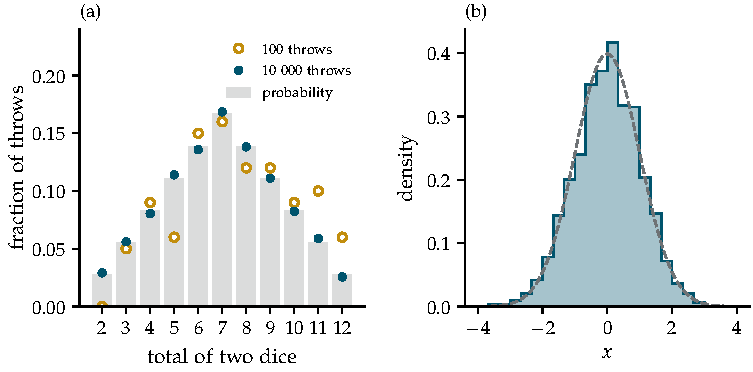
\includegraphics{ch12_ensembles/probability}
\caption{Frequencies settle on probabilities. (a) The fraction of throws
of two dice giving each total, after 100 throws (open) and 10\,000 throws
(filled), against the probabilities (bars). (b) The histogram of 1000
numbers drawn from the normal distribution, as a density, against the
Gaussian of mean 0 and standard deviation 1 (dashed).}
\label{fig:sm-probability}
\end{figure}

\subsection*{Averages and spreads}

\begin{toolbox}[Expectation and variance]
A quantity $x$ that takes the value $x_k$ with probability $\mathcal{P}_k$
has the expectation, or mean, $\ens{x} = \sum_kx_k\mathcal{P}_k$, the value
its average over many trials settles towards, and any function of it the
expectation $\ens{f(x)} = \sum_kf(x_k)\mathcal{P}_k$. The variance
measures the spread about the mean,
\begin{align*}
   \operatorname{var}(x) = \ens{(x - \ens{x})^2}
   &= \ens{x^2 - 2\ens{x}\,x + \ens{x}^2}\\
   &= \ens{x^2} - 2\ens{x}\ens{x} + \ens{x}^2 = \ens{x^2} - \ens{x}^2 ,
\end{align*}
expanding the square and then averaging term by term, which uses three
properties of $\sum_kf(x_k)\mathcal{P}_k$: the expectation of a sum is the
sum of the expectations, a constant factor such as $\ens{x}$ comes
outside, and a constant $c$ averages to $c\sum_k\mathcal{P}_k = c$. Its
square root is the standard deviation $\sigma_x$, in the units of
$x$ (written with the quantity as a subscript, to keep it apart from the
Lennard-Jones distance $\sigma$). For independent $x$ and $y$ the
probability of each pair is the product, so
\begin{equation*}
   \ens{xy} = \sum_{k,l}x_ky_l\,\mathcal{P}(x_k)\,\mathcal{P}(y_l)
   = \Bigl(\sum_kx_k\mathcal{P}(x_k)\Bigr)\Bigl(\sum_ly_l\mathcal{P}(y_l)\Bigr)
   = \ens{x}\ens{y} ,
\end{equation*}
and by the same expansion with $x + y$ in place of $x$,
\begin{align*}
   \operatorname{var}(x + y) &= \ens{x^2} + 2\ens{xy} + \ens{y^2}
   - \ens{x}^2 - 2\ens{x}\ens{y} - \ens{y}^2\\
   &= \operatorname{var}(x) + \operatorname{var}(y)
   + 2\bigl(\ens{xy} - \ens{x}\ens{y}\bigr)
   = \operatorname{var}(x) + \operatorname{var}(y) :
\end{align*}
the variances of independent quantities add.
\end{toolbox}

One die has the mean $(1 + 2 + \dotsb + 6)/6 = 3.5$ and the variance
$35/12$ (\cref{ex:sm-die}); two independent dice have twice each, 7 and
$35/6 = 5.8333$, and the 10\,000 throws above give 6.997 and 5.846.

\subsection*{Densities}

A velocity or a position takes a continuum of values, and the probability
of any exact value is zero. It has instead a probability density
$\mathcal{P}(x)$: the probability that $x$ lies between $a$ and $b$ is
$\int_a^b\mathcal{P}(x)\,\dd x$, so a narrow range of width $\Delta x$ at
$x$ holds the probability $\mathcal{P}(x)\,\Delta x$. Cutting all the
values into such ranges and letting them narrow, the sums above become
integrals: $\int\mathcal{P}\,\dd x = 1$ over all values, and $\ens{f(x)} =
\int f(x)\,\mathcal{P}(x)\,\dd x$. A histogram estimates a density: the fraction of
samples in a bin of width $\Delta x$, divided by $\Delta x$, approaches
$\mathcal{P}(x)$ as the samples grow many and the bins narrow. The most
important density of the book is the Gaussian, or normal, density,
\begin{equation}
   \mathcal{P}(x) = \frac{1}{\sigma_x\sqrt{2\pi}}\,
   \mathrm{e}^{-(x - \ens{x})^2/(2\sigma_x^2)} .
   \label{eq:sm-gauss}
\end{equation}
Its integral is 1, by the Gaussian integral $\int\mathrm{e}^{-au^2}\dd u =
\sqrt{\pi/a}$ of \cref{sec:md-ewald} with $u = x - \ens{x}$ and $a =
1/(2\sigma_x^2)$ (\cref{ex:md-normal}). It is symmetric about $\ens{x}$: the values
$\ens{x} + u$ and $\ens{x} - u$ have the same density, so their deviations
from $\ens{x}$ cancel in the average, and $\ens{x}$ is its mean. Its variance follows by integration by parts
(\cref{sec:la-euler}), with $u = x - \ens{x}$, $s = \sigma_x$, $f = u$
and $g' = u\,\mathrm{e}^{-u^2/(2s^2)}$, whose integral is $g =
-s^2\mathrm{e}^{-u^2/(2s^2)}$, as the chain rule confirms:
\begin{align*}
   \int u^2\mathrm{e}^{-u^2/(2s^2)}\dd u
   &= \Bigl[-s^2u\,\mathrm{e}^{-u^2/(2s^2)}\Bigr]_{-\infty}^{\infty}
   + s^2\int\mathrm{e}^{-u^2/(2s^2)}\dd u\\
   &= 0 + s^2\times s\sqrt{2\pi} ,
\end{align*}
and the bracket vanishes at both ends, where the exponential falls faster
than $u$ grows; dividing by $s\sqrt{2\pi}$, the variance is $\sigma_x^2$.
The fraction of the probability within $k$ standard deviations of the mean
follows with $w = u/(\sigma_x\sqrt2)$, so that $\dd u = \sigma_x\sqrt2\,\dd
w$ and the limits $\pm k\sigma_x$ become $\pm k/\sqrt2$:
\begin{equation*}
   \frac{1}{\sigma_x\sqrt{2\pi}}\int_{-k\sigma_x}^{k\sigma_x}
   \mathrm{e}^{-u^2/(2\sigma_x^2)}\,\dd u
   = \frac{1}{\sqrt\pi}\int_{-k/\sqrt2}^{k/\sqrt2}\mathrm{e}^{-w^2}\,\dd w
   = \operatorname{erf}(k/\sqrt2) ,
\end{equation*}
the last step since $\mathrm{e}^{-w^2}$ takes the same value at $w$ and
$-w$, with the error function of \cref{sec:md-ewald}: 68.27\%, 95.45\% and
99.73\% for $k$ = 1, 2 and 3.
The function \texttt{rng.normal} that drew the starting velocities of
\cref{sec:md-start} returns numbers with this density, mean 0 and
standard deviation 1; \cref{fig:sm-probability}(b) draws 1000 of them,
whose mean is 0.0029 and standard deviation 1.0115, and whose histogram
departs from \cref{eq:sm-gauss} by up to 0.042 per unit. Why velocities
should be Gaussian at all is the subject of \cref{sec:sm-maxwell}.

\begin{keyidea}
A probability is the long-run fraction of trials with an outcome; the
probabilities of independent outcomes multiply. A quantity has a mean
$\ens{x}$ and a variance $\ens{x^2} - \ens{x}^2$, and the variances of
independent quantities add. A continuous quantity has a density, which a
histogram estimates; the Gaussian density of \cref{eq:sm-gauss} has mean
$\ens{x}$ and variance $\sigma_x^2$.
\end{keyidea}

\notebook{12}{throw dice and draw normal numbers, and watch the histograms settle}

\begin{selfcheck}
What is the probability that two dice total at least 10?
\end{selfcheck}

%=============================================================================!
% 12.2  MANY STATES, ONE SYSTEM                                               !
%=============================================================================!
\section{Many states, one system}
\label{sec:sm-ergodic}

A simulation follows one system along one trajectory, and its averages
are averages over time. Statistical mechanics computes averages over the
states the system could be in, weighted by their probabilities. This
section sets out the two kinds of average and the assumption that they
agree, and then shows systems for which they do not.

\subsection*{Microstates, macrostates and ensembles}

The state of $N$ atoms is a point $\Gamma = (\vb{r}^N, \vb{p}^N)$ of phase
space (\cref{sec:ha-equations}), called a microstate. What is measured of
a macroscopic sample, its energy, volume and number of atoms, or its
temperature and pressure, fixes a macrostate, which an enormous number of
microstates share. An ensemble is the cloud of copies of \cref{sec:ha-liouville}:
many imagined copies of the system, all in the same macrostate and spread
over its microstates, with a probability density $\mathcal{P}(\Gamma)$ in phase
space: a small box of phase space, of volume $\dd\Gamma$, the product of
its $6N$ sides, holds the fraction $\mathcal{P}(\Gamma)\,\dd\Gamma$ of the
copies. The ensemble average of a quantity $A(\Gamma)$ is
\begin{equation*}
   \ens{A} = \int A(\Gamma)\,\mathcal{P}(\Gamma)\,\dd\Gamma ,
\end{equation*}
an integral over all $6N$ coordinates and momenta, the limit of a sum
over such boxes, as for the volume integrals of \cref{sec:md-ewald}, and
the time average
along one trajectory is
\begin{equation*}
   \overline{A} = \lim_{t_{\mathrm f}\to\infty}\frac{1}{t_{\mathrm f}}
   \int_0^{t_{\mathrm f}}A\bigl(\Gamma(t)\bigr)\,\dd t .
\end{equation*}
\Cref{sec:ha-liouville} showed that a cloud whose density depends on the
state only through its energy, $\mathcal{P} = f(H)$, does not change as the
copies move. The ensembles of statistical mechanics are such clouds, and
the hypothesis that makes them useful to a simulation is the ergodic
hypothesis: that a single trajectory, followed long enough, passes near
every microstate of its energy, spending equal times near equal volumes of
phase space at that energy, so that $\overline{A}$ equals $\ens{A}$ for
the ensemble spread evenly over those states (\cref{sec:sm-micro}). It can be tested, and it fails for some systems.

\subsection*{A chain that never shares}

$N$ atoms of unit mass sit in a line between two fixed walls, each joined
to its neighbours by springs of unit stiffness. With $q_j$ the displacement
of atom $j$ and $q_0 = q_{N+1} = 0$ at the walls, the spring on the left
of atom $j$ is stretched by $q_j - q_{j-1}$ and pulls it back with
$-(q_j - q_{j-1})$, and the spring on its right is stretched by $q_{j+1} -
q_j$ and pulls it on with $q_{j+1} - q_j$, as for the carts of
\cref{sec:os-modes}; together they pull it with the force $q_{j-1} - 2q_j
+ q_{j+1}$. A normal mode has every atom moving as $u_j\cos(\omega t +
\phi)$, with the acceleration $-\omega^2u_j\cos(\omega t + \phi)$, which
for unit mass must equal the force; cancelling the common factor
$\cos(\omega t + \phi)$, this needs
\begin{equation*}
   -\omega^2u_j = u_{j-1} - 2u_j + u_{j+1} .
\end{equation*}
With $u_j = \sin j\theta$, the addition formulae (\cref{eq:mo-addition})
give $u_{j-1} + u_{j+1} = \sin(j\theta - \theta) + \sin(j\theta + \theta)
= 2\sin j\theta\cos\theta$, so the condition holds with
\begin{equation*}
   \omega^2 = 2 - 2\cos\theta = 4\sin^2\tfrac12\theta ,
\end{equation*}
using $1 - \cos\theta = 2\sin^2\frac12\theta$ (\cref{ex:mo-identity}).
The wall at $j = 0$ is met, since $\sin0 = 0$, and the one at $j = N + 1$
needs $\sin(N + 1)\theta = 0$, so $\theta = k\pi/(N + 1)$ for a whole
number $k$. The values $k = 1$ to $N$ give $N$ different patterns, as many
as the chain has modes (\cref{sec:os-modes}); $k = N + 1$ gives $\sin
j\pi = 0$ for every atom, no motion at all, and larger $k$ give the same
patterns again, up to sign. The modes have the angular frequencies
$\omega_k = 2\sin(k\pi/(2N + 2))$, the positive root, since $k\pi/(2N +
2)$ lies between 0 and $\pi/2$. For $N =
32$, the slowest repeats every 66.0 units of time and the fastest every
3.15. As \cref{sec:os-modes} showed, every motion of the harmonic chain
is a sum of normal modes, each keeping its own amplitude, so a chain
started with its energy in one mode keeps it there for ever: two starts
with the same energy $E$, one in the first mode and one in the second,
give the energy in the first mode the time averages $E$ and 0. The
harmonic chain is not ergodic.

Real bonds are not perfect springs. Adding an energy $\frac13\alpha x^3$
to each spring stretched by $x$ couples the modes, and the question is
whether the coupling spreads the energy among them. Fermi, Pasta and Ulam
asked it in what Dauxois calls the first numerical experiment, programmed
and run by Mary Tsingou\cite{Dauxois2008}. \Cref{fig:sm-ergodic}(a) repeats
it with \texttt{mdlab.chain}, for 32 atoms with $\alpha = 0.25$ and the
energy 0.0724 put into the first mode, followed by velocity Verlet with
steps of 0.05, over which the total energy varies by no more than
$\num{4.9e-5}$ of itself. The first mode's share falls below 0.1 by $t = 3950$, the
energy passing to modes 2, 3 and 4 and back, and by $t = 10\,225$ it has
returned to 0.981. Over the whole run, to $t = 20\,000$, about 300
periods of the first mode, modes 5 to 32 never hold more than 0.198 of the
energy; spread equally, they would hold $28/32 = 0.875$. A trajectory
started in this special state keeps its energy in the few slowest modes,
passing it among them and back to the first, for the whole run; a run a
hundred times longer, to $t = \num{2e6}$, still leaves only 0.086 of it on
average in modes 5 to 32, and never more than 0.220.

\begin{figure}[htb]
\centering
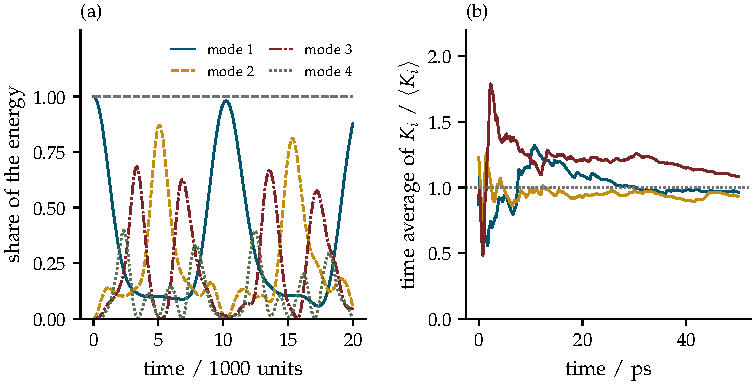
\includegraphics{ch12_ensembles/ergodic}
\caption{Time averages. (a) A chain of 32 atoms started with its energy
in the first normal mode: the share of the energy in modes 1 to 4 against
time, with the coupling $\alpha = 0.25$ (the four labelled curves), and for
the harmonic chain, whose first mode keeps all of it (grey dashed). (b) Liquid argon, 256
atoms: the running time average of the kinetic energy of three single
atoms, divided by the average over all atoms and times (dotted at 1).}
\label{fig:sm-ergodic}
\end{figure}

\subsection*{Time averages in a liquid}

The liquid provides a contrasting test over a finite observation time. \Cref{fig:sm-ergodic}(b) follows 256 atoms
of liquid argon, the model of \cref{sec:md-loop} at the density
$0.8\sigma^{-3}$ and about \SI{135}{\kelvin} (a temperature in the sense of
\cref{sec:sm-equipartition}), prepared as in
\cref{sec:cs-water}, for \SI{50}{\pico\second} at fixed energy. The
running time average of one atom's kinetic energy wanders at first and
then settles towards the average over all atoms and saved times. If
the atoms sample the same stationary distribution, this pooled average
estimates the ensemble average: after
\SI{50}{\pico\second} the time averages of the 256 atoms lie between 0.807
and 1.249 of it, with a standard deviation of 0.076. They are still
settling, and how long a run must be for an average to be trusted is the
question of Chapter~15. A crystal at a low temperature, whose
vibrations are nearly harmonic, is closer to the chain than to the
liquid, and sharing in it can be correspondingly slow.

\begin{practice}
A run that starts in a special state, such as a crystal on its lattice or
energy given to one motion only, may keep the memory of that start. The
start should be one the system could reach from many others, and its
averages should not depend on which of several such starts is used.
\end{practice}

\begin{keyidea}
An ensemble is a cloud of copies of a system with a density $\mathcal{P}(\Gamma)$
in phase space, and $\ens{A}$ its average; a simulation measures the time
average $\overline{A}$. The ergodic hypothesis, that the two agree, is
consistent with liquid argon over \SI{50}{\pico\second}; it fails for the
harmonic chain, whose modes never share energy. The chain of Fermi,
Pasta, Ulam and Tsingou also fails to share its energy equally over the
observation times tested here, returning much of it to the first mode;
that finite-time result does not establish its behaviour at infinite time.
\end{keyidea}

\notebook{12}{run the chain with any coupling and watch the modes share or not}

\begin{selfcheck}
Why is the period of the fastest mode of a long chain close to $\pi$?
\end{selfcheck}

%=============================================================================!
% 12.3  COUNTING STATES AT FIXED ENERGY                                       !
%=============================================================================!
\section{Counting states at fixed energy}
\label{sec:sm-micro}

A system that exchanges nothing with its surroundings keeps its energy,
as the runs of Chapters~9 to~11 did. This section gives the ensemble of
such a system, defines its entropy by counting its states, and finds that
temperature is what two systems sharing energy come to have in common.

\subsection*{The microcanonical ensemble}

Of all the clouds $\mathcal{P} = f(H)$ that the motion leaves unchanged, an
isolated system with energy $E$ calls for the one spread evenly over the
states of that energy, those with $H$ between $E$ and $E + \delta E$ for a
small $\delta E$, and zero elsewhere. If the system is ergodic, its
trajectory spends equal times near equal volumes of that shell, so the
even spread is the one its time averages sample. This is the
microcanonical ensemble. The volume of the shell, $\Omega(E)$, measured in
some fixed unit of phase-space volume, whose choice adds only a constant
to $S$,
counts the microstates of energy $E$ (it is not the bold matrix
$\boldsymbol\Omega$ of \cref{sec:in-reversal}), and Boltzmann's entropy is
\begin{equation}
   S = \kB\ln\Omega ,
   \label{eq:sm-entropy}
\end{equation}
with Boltzmann's constant $\kB = \SI{8.617333262e-5}{\electronvolt\per
\kelvin}$, the value SciPy gives. Taking the logarithm turns the counts of
two independent systems, which multiply, into entropies, which add.

\subsection*{Sharing energy}

Two systems placed in contact exchange energy, the total $E = E_1 + E_2$
staying fixed. Every microstate of the first combines with every
microstate of the second, so the pair has $\Omega_1(E_1)\,\Omega_2(E -
E_1)$ microstates in which the first holds $E_1$, and in the
microcanonical ensemble of the pair the probability of that division is
proportional to this number. The most probable division makes it largest,
or its logarithm, $\ln\Omega_1(E_1) + \ln\Omega_2(E - E_1)$, largest, which is
the same division since the logarithm rises whenever its argument does;
this needs its derivative with respect to $E_1$ to vanish:
\begin{equation*}
   \frac{\dd\ln\Omega_1}{\dd E_1} - \frac{\dd\ln\Omega_2}{\dd E_2} = 0 ,
\end{equation*}
by the chain rule, with $E_2 = E - E_1$ and $\dd E_2/\dd E_1 = -1$. The
two systems end where each has the same value of $\dd\ln\Omega/\dd E$,
which is therefore what they have in common in equilibrium. We call it
$1/\kB T$:
\begin{equation}
   \frac{1}{\kB T} = \frac{\dd\ln\Omega}{\dd E} , \qquad\text{or}\qquad
   \frac1T = \frac{\dd S}{\dd E} ,
   \label{eq:sm-temperature}
\end{equation}
which defines the temperature $T$, in kelvin. When the first system's
$\dd\ln\Omega/\dd E$ is the larger, moving energy into it raises the
product, so energy flows from the system with the smaller $1/T$, the
hotter one, to the colder, as it is found to.

\subsection*{The ideal gas}

$N$ atoms of mass $m$ in a box of volume $V$, with no forces between them,
have the energy $E = \sum_i\lvert\vb{p}_i\rvert^2/2m$ whatever their
positions. Each atom can be anywhere in the box, so the positions
contribute the factor $V^N$. The momenta with energy below $E$ are those
with $p_1^2 + p_2^2 + \dotsb + p_{3N}^2 \le 2mE$, listing all $3N$
components; by Pythagoras' theorem extended to $3N$ directions, these are
the points within the distance $R = \sqrt{2mE}$ of the origin, the inside
of a sphere of radius $R$ in $3N$ dimensions. That sphere is the sphere of
radius 1 with every coordinate stretched by the factor $R$, and
stretching all $3N$ coordinates by $R$ multiplies the volume of every
small box, the product of its $3N$ sides, by $R^{3N}$, so the volume
inside it is $cR^{3N}$, with $c$ the volume inside the sphere of radius 1,
a number that depends only on the dimension.
The number of states with energy below $E$ is therefore $cV^N(2mE)^{3N/2}$,
and those between $E$ and $E + \delta E$ number its derivative times
$\delta E$:
\begin{align*}
   \Omega(E) &= c\,V^N(2m)^{3N/2}\,\tfrac{3N}{2}E^{3N/2 - 1}\,\delta E ,\\
   \ln\Omega &= \bigl(\tfrac{3N}{2} - 1\bigr)\ln E + \text{a constant} ,\\
   \frac{1}{\kB T} &= \frac{3N/2 - 1}{E} \approx \frac{3N}{2E}
   && \text{by \cref{eq:sm-temperature}, for large $N$.}
\end{align*}
The third line uses the slope $1/E$ of $\ln E$: differentiating
$\mathrm{e}^{\ln E} = E$ by the chain rule gives $E\,\dd(\ln E)/\dd E =
1$.
The energy of the gas is $E = \frac32N\kB T$: $\frac32\kB T$ for each atom,
$\frac12\kB T$ for each direction of its motion, a sharing that
\cref{sec:sm-equipartition} finds to hold far more widely.

\subsection*{How sharp the sharing is}

Two such gases of $N$ atoms each, sharing $E$, have $\Omega_1\Omega_2
\propto E_1^{3N/2}(E - E_1)^{3N/2}$ for large $N$, so the probability that
the first holds the fraction $x = E_1/E$ of the energy is proportional to
$x^{3N/2}(1 - x)^{3N/2}$. It is largest at $x = \frac12$, equal energies
and equal temperatures, and \cref{fig:sm-sharing} shows how it narrows as
$N$ grows. Near the peak, the Taylor series of its logarithm
(\cref{sec:mo-taylor}) gives its width:
\begin{align*}
   \ln\mathcal{P} &= \tfrac{3N}{2}\bigl[\ln x + \ln(1 - x)\bigr]
   + \text{a constant} ,\\
   \frac{\dd\ln\mathcal{P}}{\dd x} &= \tfrac{3N}{2}\Bigl[\frac1x
   - \frac1{1 - x}\Bigr] = 0
   && \text{at $x = \tfrac12$,}\\
   \frac{\dd^2\ln\mathcal{P}}{\dd x^2} &= -\tfrac{3N}{2}\Bigl[\frac1{x^2}
   + \frac1{(1 - x)^2}\Bigr] = -12N
   && \text{at $x = \tfrac12$,}\\
   \ln\mathcal{P} &\approx \text{a constant} - \tfrac12\times12N
   \bigl(x - \tfrac12\bigr)^2 ,
\end{align*}
the chain rule giving the slope $-1/(1 - x)$ of $\ln(1 - x)$, and the
last line being the Taylor series to second order, whose first-order term
is zero at the peak. That last line is the logarithm of a Gaussian,
\cref{eq:sm-gauss}, with
$1/(2\sigma_x^2) = 6N$: the share has the standard deviation $\sigma_x =
1/\sqrt{12N}$. For 100 atoms in each gas that is 0.0289, against 0.0288
for the curve of \cref{fig:sm-sharing}, which counts the states in full,
computed numerically; for a thousand, 0.0091; for a macroscopic sample of
$10^{23}$ atoms, $\num{9e-13}$. A sample large enough to see is never
found far from its most probable division, which is why its temperature
is a definite number.

\begin{figure}[htb]
\centering
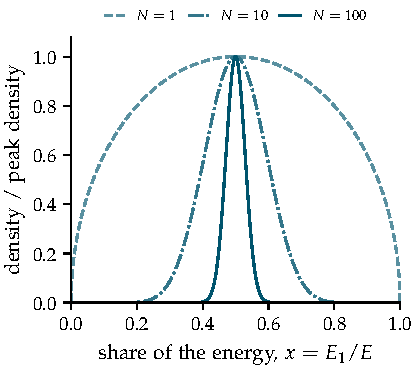
\includegraphics{ch12_ensembles/sharing}
\caption{Two gases of $N$ atoms each sharing a fixed energy: the
probability density for the first to hold the fraction $x$ of it, proportional to
$x^{3N/2 - 1}(1 - x)^{3N/2 - 1}$ by the full count $\Omega \propto
E^{3N/2 - 1}$, each curve divided by its largest value, for $N$ = 1, 10
and 100.}
\label{fig:sm-sharing}
\end{figure}

\begin{keyidea}
An isolated system, if it is ergodic, samples its energy shell evenly; the volume
$\Omega(E)$ of the shell counts its states, and $S = \kB\ln\Omega$ is its
entropy. Two systems sharing energy settle at the division with the most
states, where $\dd\ln\Omega/\dd E$, which defines $1/\kB T$, is the same
for both. An ideal gas holds $\frac32\kB T$ per atom, and the division of
energy between large systems is sharp, with a relative spread of order
$1/\sqrt N$.
\end{keyidea}

\notebook{12}{share energy between two gases of any size}

\begin{selfcheck}
For two gases of 10 atoms each, what does $1/\sqrt{12N}$ give for the
standard deviation of the share?
\end{selfcheck}

%=============================================================================!
% 12.4  A SYSTEM AND ITS BATH                                                 !
%=============================================================================!
\section{A system and its bath}
\label{sec:sm-canonical}

Most systems of interest are not isolated: a sample exchanges energy with
its container, and a few hundred atoms in a simulation stand for a small
part of a much larger piece of matter. This section finds the
probabilities of the states of a system kept in contact with a much
larger one, its bath, and with them the partition function from which
averages and fluctuations follow.

\subsection*{The Boltzmann factor}

\begin{figure}[htb]
\centering
\begin{tikzpicture}[line cap=round, line join=round]
   \draw[line width=0.8pt, fill=black!6] (0,0) rectangle (6.4,2.6);
   \draw[line width=0.8pt, fill=white] (2.4,0.7) rectangle (4.0,1.9);
   \node[align=center] at (3.2,1.3) {system\\[2pt]\small $E_s$};
   \node[align=center] at (1.1,1.3) {bath\\[2pt]\small $E - E_s$};
   \node at (5.3,1.3) {\small energy};
   \draw[-{Stealth[length=5pt]}, line width=0.8pt, accent]
      (4.05,1.55) -- (4.75,1.55);
   \draw[{Stealth[length=5pt]}-, line width=0.8pt, accent]
      (4.05,1.05) -- (4.75,1.05);
\end{tikzpicture}
\caption{A small system inside a large bath. The two together are
isolated, with energy $E$; the system holds $E_s$ and the bath the rest,
and energy passes between them.}
\label{fig:sm-bath}
\end{figure}

The system and its bath (\cref{fig:sm-bath}) together are isolated, with
the energy $E$, so the pair is microcanonical: all its microstates of
energy $E$ are equally likely. We fix one microstate of the system, with
energy $E_s$. The bath then holds $E - E_s$, in any of its
$\Omega_{\mathrm B}(E - E_s)$ microstates, so the probability of that one
microstate of the system is proportional to $\Omega_{\mathrm B}(E - E_s)$.
The system's energy is small against the bath's, so we expand about $E$
in a Taylor series. $\Omega_{\mathrm B}$ itself changes enormously with its
energy, roughly as $E^{3N/2}$ for an ideal gas (\cref{sec:sm-micro}), but
its logarithm changes slowly, so it is the logarithm we expand:
\begin{align*}
   \ln\Omega_{\mathrm B}(E - E_s) &= \ln\Omega_{\mathrm B}(E)
   - E_s\,\frac{\dd\ln\Omega_{\mathrm B}}{\dd E}
   + \tfrac12E_s^2\,\frac{\dd^2\ln\Omega_{\mathrm B}}{\dd E^2} - \dotsb\\
   &= \ln\Omega_{\mathrm B}(E) - \frac{E_s}{\kB T} + \dotsb ,
\end{align*}
the second line by \cref{eq:sm-temperature}, with $T$ the temperature of
the bath. The second derivative is the rate
at which $\dd\ln\Omega_{\mathrm B}/\dd E = 1/\kB T$ changes, $-(1/\kB
T^2)\,\dd T/\dd E$ by the chain rule, so the next term is
$-\frac12E_s^2(\dd T/\dd E)/\kB T^2$; divided by the term kept,
$-E_s/\kB T$, it gives the ratio $\frac12E_s(\dd T/\dd E)/T$, in which
$\dd T/\dd E$ is how far the bath's temperature rises per unit of energy
it gains. For a bath that is an ideal gas, $T = 2E/3N\kB$ gives $\dd
T/\dd E = 2/3N\kB = T/E$, and the ratio is $E_s/2E$, half the system's
share of the energy: negligible for a bath much larger than the system
(\cref{ex:sm-bath}), and the dropped term itself, $(E_s/\kB T)(E_s/2E)$,
is small when $E \gg E_s^2/\kB T$. The factor $\Omega_{\mathrm B}(E)$ is the same for
every microstate of the system and joins the constant of proportionality,
so, taking the exponential of both sides,
\begin{equation}
   \mathcal{P}(\text{microstate}) \propto \mathrm{e}^{-E_s/\kB T}
   = \mathrm{e}^{-\beta E_s} , \qquad \beta = \frac{1}{\kB T} :
   \label{eq:sm-boltzmann}
\end{equation}
the probability of a state of the system falls exponentially with its
energy, by the Boltzmann factor. The bath enters only through its
temperature. The ensemble of a system at fixed $N$, $V$ and $T$ with these
probabilities is the canonical ensemble.

\subsection*{The partition function}

The probabilities must add up to one, so the probability of microstate
$s$ is $\mathcal{P}_s = \mathrm{e}^{-\beta E_s}/Z$, with $Z$ the sum over
all the system's microstates, or for the continuous phase space of
classical atoms the integral over it, the partition function:
\begin{equation}
   Z = \sum_s\mathrm{e}^{-\beta E_s} , \qquad\text{or}\qquad
   Z = \int\mathrm{e}^{-\beta H(\Gamma)}\,\dd\Gamma .
   \label{eq:sm-partition}
\end{equation}
with $\dd\Gamma$ measured in the unit of phase-space volume of
\cref{sec:sm-micro}, so that $Z$ is a pure number; changing that unit
adds a constant to $S$ and $\kB T$ times a constant to $F$, which drop out
of every difference and derivative below.
Averages follow from it by differentiation with respect to $\beta$:
\begin{align*}
   -\frac{\dd\ln Z}{\dd\beta} &= -\frac1Z\,\frac{\dd Z}{\dd\beta}
   = \frac{1}{Z}\sum_sE_s\mathrm{e}^{-\beta E_s} = \ens{E} ,\\
   \frac{\dd^2\ln Z}{\dd\beta^2} &= -\frac{\dd\ens{E}}{\dd\beta}
   = \frac{1}{Z}\sum_sE_s^2\mathrm{e}^{-\beta E_s}
   - \Bigl(\frac1Z\sum_sE_s\mathrm{e}^{-\beta E_s}\Bigr)^2
   = \ens{E^2} - \ens{E}^2 ,
\end{align*}
the first by the chain rule, with $\dd Z/\dd\beta = -\sum_sE_s
\mathrm{e}^{-\beta E_s}$, and the second by the product rule
(\cref{sec:ne-drag}) applied to $\ens{E} = (1/Z)\sum_sE_s
\mathrm{e}^{-\beta E_s}$: the sum has the derivative $-\sum_sE_s^2
\mathrm{e}^{-\beta E_s}$, and $1/Z$, by the chain rule, the derivative
$-(1/Z^2)\,\dd Z/\dd\beta = (1/Z^2)\sum_sE_s\mathrm{e}^{-\beta E_s}$.
The energy of a system in contact with a bath fluctuates, and its
variance is the rate at which $-\ens{E}$ changes with $\beta$. The heat
capacity $C_V = \dd\ens{E}/\dd T$ is the energy taken up per degree, at
fixed volume. By the chain rule $C_V = (\dd\ens{E}/\dd\beta)(\dd\beta/\dd
T)$, and $\dd\beta/\dd T = -1/(\kB T^2)$, so
\begin{equation}
   \ens{E^2} - \ens{E}^2 = -\frac{\dd\ens{E}}{\dd\beta}
   = \kB T^2\,C_V .
   \label{eq:sm-fluctuation}
\end{equation}
The size of the energy's fluctuations measures how much energy the
system takes up when warmed. The free energy is defined by
\begin{equation*}
   F = -\kB T\ln Z ,
\end{equation*}
and equals $\ens{E} - TS$ with the entropy $S = -\kB\sum_s\mathcal{P}_s\ln
\mathcal{P}_s$, which for the equal probabilities $1/\Omega$ of the
microcanonical ensemble is \cref{eq:sm-entropy} (\cref{ex:sm-free}).

\subsection*{A spring, and the odds of a hop}

One coordinate on a spring, $H = p^2/2m + \frac12kx^2$, has, by the
Gaussian integral of \cref{sec:md-ewald} twice,
\begin{equation*}
   Z = \int\mathrm{e}^{-\beta p^2/2m}\dd p\int\mathrm{e}^{-\beta kx^2/2}
   \dd x = \sqrt{\frac{2\pi m}{\beta}}\sqrt{\frac{2\pi}{\beta k}}
   = \frac{2\pi}{\beta\omega} ,
\end{equation*}
with $\omega = \sqrt{k/m}$. Then $\ln Z = -\ln\beta + \text{a constant}$,
and $\ens{E} = -\dd\ln Z/\dd\beta = 1/\beta = \kB T$: a classical vibration holds
$\kB T$ on average, whatever its stiffness, which makes precise the
`typical energy of order $\kB T$' of \cref{sec:pe-classical}. At
\SI{300}{\kelvin}, $\kB T = \SI{0.02585}{\electronvolt}$.

The Boltzmann factor also answers the question of \cref{sec:en-surface},
how often an atom reaches the top of its barrier. The kinetic energy
depends on the momenta alone and $U$ on the positions alone, so
$\mathrm{e}^{-\beta H}$ is $\mathrm{e}^{-\beta U}$ times a factor of the
momenta, and integrating over the momenta turns that factor into a number
that is the same at every position. The positions are left with the
density $\mathrm{e}^{-\beta U}$, in which the masses no longer appear, as
\cref{sec:cs-mass} anticipated: of two places whose potential energies
differ by $\Delta U$, an atom is found near the higher, per unit volume,
$\mathrm{e}^{-\Delta U/\kB T}$ times as often as near the lower. For the
lithium atom of that model, which moves over the surface, the density is
per unit area, and at the bridge, \SI{0.3}{\electronvolt} above its
hollow, the odds are $\mathrm{e}^{-0.3/0.02585} = \num{9.1e-6}$ at
\SI{300}{\kelvin}, and $\num{3.0e-3}$ at \SI{600}{\kelvin}, 331 times
larger: a barrier that is rarely reached at room temperature is reached
hundreds of times as often when the temperature doubles. For an atom
moving in two directions the same number is also the probability that its
kinetic energy is at least the barrier, since its kinetic energy has the
density $\mathrm{e}^{-K/\kB T}/\kB T$ (\cref{sec:sm-kinetic}). How often an atom actually hops depends also on how
often it tries, which Chapters~16 and~17 measure.

\begin{keyidea}
A system in contact with a bath at temperature $T$ is found in a
microstate of energy $E_s$ with a probability proportional to
$\mathrm{e}^{-E_s/\kB T}$. The partition function $Z$ normalises the
probabilities; $\ens{E} = -\dd\ln Z/\dd\beta$, the energy's variance is
$\kB T^2C_V$, and $F = -\kB T\ln Z$. A classical vibration holds $\kB T$
on average.
\end{keyidea}

\notebook{12}{set a barrier and a temperature and read off the odds}

\begin{selfcheck}
What are the odds of the \SI{0.3}{\electronvolt} barrier at
\SI{100}{\kelvin}?
\end{selfcheck}

%=============================================================================!
% 12.5  THE DISTRIBUTION OF VELOCITIES                                        !
%=============================================================================!
\section{The distribution of velocities}
\label{sec:sm-maxwell}

\Cref{sec:md-start} drew starting velocities from the normal distribution
and promised a reason. This section derives the distribution of the
velocities of atoms at a temperature $T$ from the Boltzmann factor, then
the distributions of their speeds and kinetic energies, and measures all
three in liquid argon.

\subsection*{Each component is Gaussian}

We first take an unconstrained canonical system, with no condition on its
total momentum. The energy of $N$ atoms is $H = \sum_{i,x}p_{ix}^2/2m_i + U(\vb{r}^N)$,
where the sum runs over the atoms $i$ and, with $x$ standing for each in
turn, the three directions $x$, $y$ and $z$. The
exponential of a sum is a product, so the Boltzmann factor of
\cref{eq:sm-boltzmann} splits into one factor for the positions and one
for each component of momentum:
\begin{equation*}
   \mathrm{e}^{-\beta H} = \mathrm{e}^{-\beta U(\vb{r}^N)}\prod_{i,x}
   \mathrm{e}^{-\beta p_{ix}^2/2m_i} .
\end{equation*}
A probability density that is a product of factors, each depending on
one quantity alone, describes quantities that are independent, so every
component of every momentum is independent of the others and of the
positions. With $p_{ix} = m_iv_{ix}$, the density of one component of
velocity is proportional to $\mathrm{e}^{-m_iv_{ix}^2/2\kB T}$, which is
the Gaussian of \cref{eq:sm-gauss} with mean zero and variance
\begin{equation}
   \sigma_v^2 = \frac{\kB T}{m_i} .
   \label{eq:sm-maxwell}
\end{equation}
This is the Maxwell-Boltzmann distribution of velocities. Two things in it
matter for simulation. It holds whatever the forces: the velocities of
atoms in a gas, a liquid or a crystal at the same temperature have the
same distribution, in classical mechanics. And the spread depends on the
mass: a lithium atom at \SI{300}{\kelvin} has $\sigma_v = \sqrt{\kB T/m} =
\sqrt{0.025852/(6.94\times103.6427)} =
\SI{0.005995}{\angstrom\per\femto\second}$, the factor 103.6427 of
\cref{eq:en-mv2} turning \si{\amu\angstrom\squared\per\femto\second\squared}
into \si{\electronvolt}, and an argon atom
\SI{0.002499}{\angstrom\per\femto\second}, smaller by $\sqrt{39.948/6.94}
= 2.399$, the ratio of the square roots of their masses. Dividing the normal numbers by
$\sqrt{m_i}$, as \texttt{starting\_velocities} of \cref{sec:md-start}
did, gives each atom this spread up to a common factor, which the
scaling to the chosen energy then fixed.

\texttt{mdlab.statmech.thermal\_velocities} draws velocities at a
temperature directly:

\begin{code}
    m = np.asarray(masses, dtype=float)
    xi = rng.standard_normal((len(m), 3))
    v = xi * np.sqrt(kb * temperature / (m * mv2_to_energy))[:, None]
    if remove_drift:
        v = v - (m @ v) / m.sum()
    return v
\end{code}

\noindent Line 2 draws $3N$ numbers of mean 0 and variance 1, and line 3
multiplies each atom's by its $\sigma_v$, with \texttt{mv2\_to\_energy}
the factor of \cref{eq:en-mv2} that turns $mv^2$ into
\si{\electronvolt}. Line 5 removes the drift of the centre of mass, as in
\cref{sec:md-start}. ASE's \texttt{thermalize\_momenta} draws the numbers
in the same order, so the same starting number of the random generator,
its seed, gives the same velocities: for 50
atoms of random masses at \SI{300}{\kelvin} they differ by at most
\num{1.7e-7} of their size. That is half the relative difference of
\num{3.4e-7} between the two libraries' values of $\kB$, ASE's being the
value recommended for the constants in 2014, since $\sigma_v$ goes as
$\sqrt{\kB}$ and a small relative change in a quantity changes its square
root by half as much.

\subsection*{Speeds and kinetic energies}

The speed $v = \lvert\vb{v}\rvert$ of an atom combines three independent
components. The probability that the velocity lies in a small box $\dd
v_x\,\dd v_y\,\dd v_z$ is the product of the three Gaussians, each with the
factor $1/(\sigma_v\sqrt{2\pi}) = (m/2\pi\kB T)^{1/2}$, times the box, and
with $v_x^2 + v_y^2 + v_z^2 = v^2$ it is
\begin{equation*}
   \Bigl(\frac{m}{2\pi\kB T}\Bigr)^{3/2}\mathrm{e}^{-mv^2/2\kB T}\,
   \dd v_x\,\dd v_y\,\dd v_z ,
\end{equation*}
which depends on the velocity only through its size. The velocities with
speeds between $v$ and $v + \dd v$ fill a spherical shell of area $4\pi
v^2$ and thickness $\dd v$, so the density of the speed is
\begin{equation}
   \mathcal{P}(v) = 4\pi v^2\Bigl(\frac{m}{2\pi\kB T}\Bigr)^{3/2}
   \mathrm{e}^{-mv^2/2\kB T} .
   \label{eq:sm-speed}
\end{equation}
The factor $v^2$ makes it zero at $v = 0$, since few velocities have all
three components near zero. It peaks at $\sqrt2\,\sigma_v$ and has the
mean $\sqrt{8/\pi}\,\sigma_v$ (\cref{ex:sm-speeds}); the mean speed of
lithium at \SI{300}{\kelvin} is \SI{0.00957}{\angstrom\per\femto\second},
or \SI{957}{\metre\per\second}, with \SI{1}{\angstrom\per\femto\second}
equal to \SI{e5}{\metre\per\second}, and that of argon
\SI{399}{\metre\per\second}.

An atom's kinetic energy $K_i = \frac12mv^2$ follows by a change of
variable. Between $K_i$ and $K_i + \dd K_i$ lie the speeds between $v$
and $v + \dd v$ with $\dd K_i = mv\,\dd v$, and the two hold the same
probability, $\mathcal{P}(K_i)\,\dd K_i = \mathcal{P}(v)\,\dd v$, so
$\mathcal{P}(K_i) = \mathcal{P}(v)/(mv)$. With $mv^2/2\kB T = K_i/\kB T$
and $v\sqrt m = \sqrt{2K_i}$,
\begin{equation*}
   \frac{\mathcal{P}(v)}{mv} = \frac{4\pi v\sqrt m}{(2\pi\kB T)^{3/2}}\,
   \mathrm{e}^{-K_i/\kB T}
   = \frac{4\pi\sqrt2}{(2\pi)^{3/2}}\,(\kB T)^{-3/2}\sqrt{K_i}\,
   \mathrm{e}^{-K_i/\kB T} ,
\end{equation*}
and $4\pi\sqrt2/(2\pi)^{3/2} = 4\pi\sqrt2/(2\sqrt2\,\pi^{3/2}) =
2/\sqrt\pi$, so
\begin{equation}
   \mathcal{P}(K_i) = \frac{2}{\sqrt\pi}\,(\kB T)^{-3/2}\sqrt{K_i}\,
   \mathrm{e}^{-K_i/\kB T} ,
   \label{eq:sm-atom-energy}
\end{equation}
the same for every mass. Its mean is $\frac32\kB T$ and its variance
$\frac32(\kB T)^2$, as \cref{sec:sm-kinetic} shows for any number of
freedoms.

\subsection*{Measured in a liquid}

\Cref{fig:sm-maxwell} tests the three densities on the liquid argon of
\cref{fig:sm-ergodic}(b), 256 atoms over \SI{50}{\pico\second}, with the
velocities saved every \SI{50}{\femto\second}: 768\,768 components from
1001 frames. The run is at fixed energy, not in contact with a bath, but
each atom has the other 255 around it, which act as its bath. The
kinetic temperature of the run, defined in \cref{sec:sm-equipartition},
is \SI{134.63}{\kelvin}, at which \cref{eq:sm-maxwell} gives $\sigma_v =
\SI{0.001674}{\angstrom\per\femto\second}$; the components have the
standard deviation \SI{0.001671}{\angstrom\per\femto\second}, and
\cref{sec:sm-equipartition} accounts for the difference. The mean speed is
\SI{0.002668}{\angstrom\per\femto\second} against 0.002671 from
\cref{eq:sm-speed}, and the kinetic energies of single atoms have the
mean $1.494\,\kB T$ and the variance $1.479\,(\kB T)^2$, against
$\frac32$ for both.

\begin{figure}[htb]
\centering
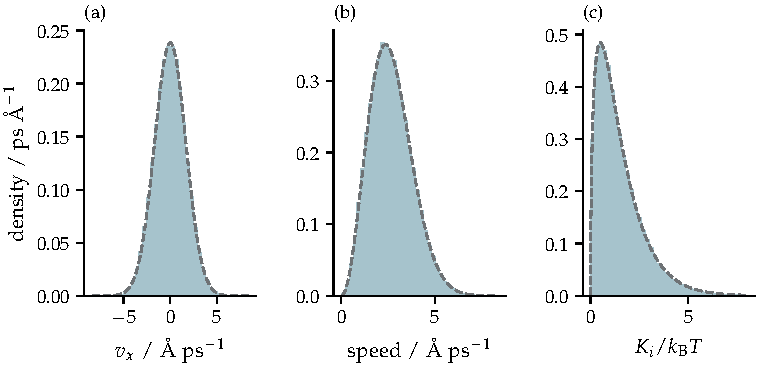
\includegraphics{ch12_ensembles/maxwell}
\caption{Velocities in liquid argon at \SI{134.6}{\kelvin}: histograms of
256 atoms over \SI{50}{\pico\second}, with velocities in
\si{\angstrom\per\pico\second}, a thousand times their values in
\si{\angstrom\per\femto\second}. (a) Every component of velocity, against
the Gaussian of variance $\kB T/m$ (dashed). (b) The speeds, against
\cref{eq:sm-speed}. (c) The kinetic energies of single atoms, in units of
$\kB T$, against \cref{eq:sm-atom-energy}, a density per unit of $\kB
T$.}
\label{fig:sm-maxwell}
\end{figure}

A Gaussian has a property that the histogram shows only roughly and a
single number shows well. The fourth moment of the Gaussian of mean zero
is $\ens{v^4} = 3\sigma_v^4$ (\cref{ex:sm-fourth}), so the excess
kurtosis
\begin{equation*}
   \frac{\ens{u^4}}{\ens{u^2}^2} - 3 ,
\end{equation*}
computed over the mass-weighted components $u = \sqrt{m}\,v$, which share
one variance $\kB T$ whatever the masses, is zero for velocities with the
Maxwell-Boltzmann distribution; pooled components of different variances
would give more than zero even if each were Gaussian. Components spread
evenly over an interval give $-1.2$ (\cref{ex:sm-fourth}). Over the
768\,768 components of the liquid it is $-0.0072$, small against the
$-1.2$ of an even spread. \texttt{mdlab.diagnostics.excess\_kurtosis}
computes it, and \cref{sec:sm-trajectory} uses it to catch velocities that
are not yet Maxwellian.

\begin{keyidea}
In the unconstrained canonical ensemble each component of each velocity
is independent and Gaussian, with mean zero and variance $\kB T/m$, whatever the forces.
The speed has the density $4\pi v^2(m/2\pi\kB T)^{3/2}\mathrm{e}^{-mv^2/
2\kB T}$, and an atom's kinetic energy a density with mean $\frac32\kB T$
for every mass. The excess kurtosis of the mass-weighted components is
zero for Maxwellian velocities. Removing the total momentum or holding
bond lengths constrains these components, as the next section explains.
\end{keyidea}

\notebook{12}{draw velocities at any temperature and mass, and check them against ASE}

\begin{selfcheck}
What is $\sigma_v$ for a lithium atom at \SI{600}{\kelvin}?
\end{selfcheck}

%=============================================================================!
% 12.6  EQUAL SHARES AND THE KINETIC TEMPERATURE                              !
%=============================================================================!
\section{Equal shares and the kinetic temperature}
\label{sec:sm-equipartition}

\Cref{sec:en-friction} said that the warmth of rubbing surfaces is the
hidden energy of their jiggling atoms. This section finds how that energy
is shared among the ways the atoms can move, and from the share of the
kinetic energy defines the temperature that a simulation measures.

\subsection*{The equipartition theorem}

We take $x$ to be any one coordinate or momentum of a system in the
canonical ensemble, whose range runs from $x_1$ to $x_2$, and require
$x\,\mathrm{e}^{-\beta H}$ to vanish at both ends, as it does for a
momentum, whose range is unbounded and where the exponential falls faster
than $x$ grows, or for a coordinate held in by a potential that rises
without limit, walls included. The average of $x$ times the slope of $H$
along it is
\begin{equation*}
   \Bigl\langle x\,\frac{\partial H}{\partial x}\Bigr\rangle
   = \frac1Z\int x\,\frac{\partial H}{\partial x}\,\mathrm{e}^{-\beta H}
   \,\dd\Gamma ,
\end{equation*}
and the integral over $x$, with every other coordinate and momentum held
fixed, can be done by parts, since by the chain rule
$\partial(\mathrm{e}^{-\beta H})/\partial x = -\beta\,(\partial H/\partial
x)\,\mathrm{e}^{-\beta H}$:
\begin{align*}
   \int_{x_1}^{x_2}x\,\frac{\partial H}{\partial x}\,\mathrm{e}^{-\beta H}
   \,\dd x
   &= -\frac1\beta\int_{x_1}^{x_2}x\,\frac{\partial(\mathrm{e}^{-\beta H})}
   {\partial x}\,\dd x\\
   &= -\frac1\beta\Bigl[x\,\mathrm{e}^{-\beta H}\Bigr]_{x_1}^{x_2}
   + \frac1\beta\int_{x_1}^{x_2}\mathrm{e}^{-\beta H}\,\dd x
   && \text{parts, with $f = x$,}\\
   &= \kB T\int_{x_1}^{x_2}\mathrm{e}^{-\beta H}\,\dd x
   && \text{the bracket vanishes.}
\end{align*}
Integrating over the other coordinates and momenta too, and dividing by
$Z = \int\mathrm{e}^{-\beta H}\,\dd\Gamma$,
\begin{equation}
   \Bigl\langle x\,\frac{\partial H}{\partial x}\Bigr\rangle = \kB T ,
   \label{eq:sm-equipartition}
\end{equation}
whatever $x$ is and whatever the rest of $H$. When $H$ contains $x$ only
through a term $\frac12ax^2$, then $x\,\partial H/\partial x = ax^2$, twice
that term, and the term has the average $\frac12\kB T$. Every term of the
energy that is the square of a coordinate or momentum appearing in no
other term holds, on average, $\frac12\kB T$, whatever its coefficient:
this is the equipartition of energy. A square whose variable appears
elsewhere too, as $x$ does in $\frac12x^2 + \frac12y^2 + cxy$, need not. Chapter~14 uses \cref{eq:sm-equipartition} for the positions to
find the pressure.

Three cases recur in this book.
\begin{itemize}
\item Each component of momentum enters $H$ as $p_{ix}^2/2m_i$, so, when
   the total momentum is free, $\ens{\frac12m_iv_{ix}^2} = \frac12\kB T$
   for every atom and direction,
   whatever its mass and whatever the forces on it. At \SI{300}{\kelvin}
   that is \SI{12.93}{\milli\electronvolt}, the share given to each
   freedom of the water of \cref{sec:cs-water}.
\item A vibration of small amplitude has $H = p^2/2m + \frac12kx^2$, two
   squares, and holds $\frac12\kB T$ as kinetic and $\frac12\kB T$ as
   potential energy, $\kB T$ in all, as \cref{sec:sm-canonical} found from
   its partition function. \Cref{sec:os-energy} found the same equal
   division as an average over one period of one oscillator; here it is an
   average over the ensemble.
\item A molecule of two atoms turning freely has, in the angle $\theta$
   of its axis from the $z$ axis and the angle $\phi$ about it, $H = p_\theta^2/2I + p_\phi^2/(2I\sin^2\theta)$
   (\cref{ex:sm-rotor}). Each term is the square of a momentum, so each
   holds $\frac12\kB T$, and the turning holds $\kB T$ in all, as
   \cref{sec:ro-molecules} assumed.
\end{itemize}
A term that is not a square does not hold $\frac12\kB T$: the potential
energy of a liquid, made of Lennard-Jones terms, has no simple share. The
kinetic energy is always a sum of squares, which is why it serves as the
thermometer.

\subsection*{The kinetic temperature}

With $N_{\mathrm f}$ freedoms, each holding $\frac12\kB T$ of kinetic
energy on average, $\ens{K} = \frac12N_{\mathrm f}\kB T$, and the
instantaneous kinetic temperature
\begin{equation}
   T_{\mathrm{kin}} = \frac{2K}{N_{\mathrm f}\kB}
   \label{eq:sm-kinetic-temperature}
\end{equation}
has the temperature $T$ as its average. It is what a simulation reports
as `the temperature' at each step; it fluctuates, by an amount
\cref{sec:sm-kinetic} finds. In an isolated system the kinetic
temperature's average differs from the $T$ of \cref{eq:sm-temperature} by
terms of order $1/N$: for the ideal gas of \cref{sec:sm-micro}, $\kB T =
E/(\frac32N - 1)$, while $2K/(3N\kB)$ with $K = E$ gives $\kB
T_{\mathrm{kin}} = E/\frac32N$, smaller by the factor $1 - 2/(3N)$.

Counting $N_{\mathrm f}$ is where errors enter. $N$ atoms have $3N$
components of velocity, and each independent restriction on them removes one.
\begin{itemize}
\item A periodic run whose drift has been removed keeps its total
   momentum at zero (\cref{sec:md-start}), so its velocities satisfy three
   conditions, $\sum_im_i\vb{v}_i = \vb{0}$, and the kinetic energy is
   shared among $3N - 3$ freedoms.
\item Each distance held by RATTLE removes the component of relative
   velocity along it (\cref{sec:cs-rattle}): $n_{\mathrm c}$ independent held distances
   remove $n_{\mathrm c}$ freedoms.
\item An isolated molecule whose turning has also been removed has three
   more conditions, or two if it is linear (\cref{sec:ro-freedom}),
   leaving $3N - 6$, or $3N - 5$.
\end{itemize}
In the mass-weighted components $u_k = \sqrt{m_k}\,v_k$, the kinetic
energy is $K = \frac12\sum_ku_k^2$, half the squared length of $\vb{u}$,
and each restriction is a condition that $\vb{u}$ be at right angles to a
direction fixed by the positions at that instant: for the drift along $x$, $\sum_i\sqrt{m_i}\,u_{ix} = 0$.
Writing $\vb{u} = \sum_kc_k\vb{e}_k$ along $3N$ directions of length 1 at
right angles to one another, the first $n$ chosen to span the directions
that $n$ restrictions fix, gives $K = \frac12\sum_kc_k^2$ as in
\cref{sec:os-modes}, with $c_1$ to $c_n$ held at zero: a sum of $3N - n$
squares, each holding $\frac12\kB T$. So a periodic run with its drift
removed has $N_{\mathrm f} = 3N - n_{\mathrm c} - 3$, which
\texttt{mdlab.statmech.degrees\_of\_freedom} returns: 765 for 256 argon
atoms, and 381 for the 64 rigid water molecules of Chapter~11.
\texttt{kinetic\_temperature} then applies \cref{eq:sm-kinetic-temperature}.

The count shows in the measurements of \cref{sec:sm-maxwell}. The
kinetic energy of 765 freedoms is spread over 768 components of
velocity, so the components' mean square is $765/768$ of $\kB T/m$, and
their standard deviation $\sqrt{765/768} = 0.99804$ of $\sigma_v$:
$0.99804\times0.001674 = \SI{0.001671}{\angstrom\per\femto\second}$, the
value measured. ASE's \texttt{get\_temperature} divides by $3N$ less the
freedoms its constraints remove, and does not take off three for the
drift. On the last frame of the liquid, \texttt{mdlab} gives
\SI{137.7961}{\kelvin} and ASE \SI{137.2579}{\kelvin}, in the ratio
0.996094, which is $765/768$; the two agree once they count alike.

\subsection*{Shares between species, and with the potential}

Equipartition gives every atom the same mean kinetic energy whatever its
mass, so the heavier atoms of a mixture move more slowly and are no
colder. A liquid of 256 atoms with argon's forces, half of mass
\SI{39.948}{\amu} and half of \SI{83.798}{\amu}, the mass of krypton,
started with velocities drawn at \SI{130}{\kelvin}, has its light atoms at
\SI{126}{\kelvin} and its heavy atoms at \SI{124}{\kelvin} over the last
\SI{10}{\pico\second} of \SI{20}{\pico\second}, each temperature counting
the three components of each atom of the species. Whether a gap of
\SI{2}{\kelvin} is a real difference or the noise of a short run is the
question of Chapter~15.

Equipartition also explains what \cref{sec:md-start} saw. A crystal
started on its lattice has no potential energy above its minimum, and its
vibrations, nearly harmonic, take half of the kinetic energy they are
given: each ends with $\frac12\kB T$ of each kind. The 500 argon atoms of
that section lost half of their kinetic energy within
\SI{0.1}{\pico\second}, and 256 atoms on their lattice at the spacing of
ASE's reference value\cite{Larsen2017}, $a = \SI{5.26}{\angstrom}$, a
little below the model's \SI{5.267}{\angstrom}, which squeezes the cell
slightly but leaves the lattice, by its symmetry, where every force
vanishes, given velocities at \SI{40}{\kelvin}
(a kinetic temperature of \SI{41.5}{\kelvin}, by the scatter of
\cref{sec:sm-kinetic}), settle at \SI{21.0}{\kelvin}, 0.506 of the start.
A liquid has no such simple ratio, since its potential energy is not a sum
of squares.

\begin{practice}
Velocities drawn at a temperature set only the kinetic energy. A crystal
started on its lattice ends near half the temperature asked for, and a
system started anywhere else ends somewhere that has to be found by
running. A run is at the temperature asked for only after that
temperature has been measured over the run; a thermostat (Chapter~13)
holds it there.
\end{practice}

\begin{keyidea}
Every term of the energy that is the square of a coordinate or momentum
appearing in no other term holds $\frac12\kB T$ on average. The kinetic energy is such a sum, which
makes $T_{\mathrm{kin}} = 2K/(N_{\mathrm f}\kB)$ a thermometer, with
$N_{\mathrm f} = 3N - n_{\mathrm c} - 3$ in a periodic run whose drift is
removed. Atoms of every mass share alike; a harmonic crystal shares
equally between kinetic and potential energy.
\end{keyidea}

\notebook{12}{count the freedoms of a run and compare the temperature with ASE's}

\begin{selfcheck}
A box of 100 rigid water molecules, drift removed, has a kinetic energy
of \SI{7.4}{\electronvolt}. What is its kinetic temperature?
\end{selfcheck}

%=============================================================================!
% 12.7  HOW MUCH THE TEMPERATURE FLUCTUATES                                   !
%=============================================================================!
\section{How much the temperature fluctuates}
\label{sec:sm-kinetic}

The kinetic temperature of a run is never still. This section derives the
distribution of the kinetic energy in the canonical ensemble, finds that
a run at fixed energy fluctuates less, and turns the difference into a
measurement of the heat capacity. Chapter~13 tests every thermostat
against the distribution found here.

\subsection*{The kinetic energy in the canonical ensemble}

In the $N_{\mathrm f}$ free components $c_k$ of
\cref{sec:sm-equipartition}, the kinetic energy is $K =
\frac12\sum_kc_k^2$. The velocities with kinetic energy below $K$ fill
the inside of a sphere of radius $\sqrt{2K}$ in $N_{\mathrm f}$
dimensions, whose volume, as for the ideal gas of \cref{sec:sm-micro}, is
a constant times $K^{N_{\mathrm f}/2}$, and those between $K$ and $K +
\dd K$ fill a shell whose volume is the derivative of that volume times
$\dd K$, a constant times $K^{N_{\mathrm f}/2 - 1}\,\dd K$. Each
velocity in the shell has the Boltzmann factor $\mathrm{e}^{-\beta K}$,
so
\begin{equation}
   \mathcal{P}(K) \propto K^{N_{\mathrm f}/2 - 1}\,\mathrm{e}^{-K/\kB T} .
   \label{eq:sm-gamma}
\end{equation}
This is the gamma distribution. For one atom, $N_{\mathrm f} = 3$, it is
the $\sqrt{K}\,\mathrm{e}^{-K/\kB T}$ of \cref{eq:sm-atom-energy}; for an
atom moving over a surface, $N_{\mathrm f} = 2$, it is
$\mathrm{e}^{-K/\kB T}/\kB T$, and the probability that $K$ is at least
some $U_{\mathrm b}$ is $\mathrm{e}^{-U_{\mathrm b}/\kB T}$. Its mean and
variance follow as in \cref{sec:sm-canonical}, applied to the kinetic
energy alone, which is independent of the positions: with $a =
N_{\mathrm f}/2$, the factor $K^{a-1}$ that counts the velocities does not depend on $\beta$, so each
derivative of the normalising integral with respect to $\beta$ brings
down a factor $-K$, as each derivative of $Z$ brought down $-E_s$. The
normalising integral is, with $s = \beta K$,
\begin{equation*}
   Z_K = \int_0^\infty K^{a - 1}\mathrm{e}^{-\beta K}\,\dd K
   = \beta^{-a}\int_0^\infty s^{a - 1}\mathrm{e}^{-s}\,\dd s ,
\end{equation*}
and the last integral is a number, the gamma function of $a$, written
$\Gamma(a)$ (no relation to the phase point $\Gamma$), which
the function \texttt{kinetic\_\allowbreak energy\_\allowbreak density}
evaluates through its logarithm. So $\ln Z_K = -a\ln\beta + \text{a
constant}$, and
\begin{equation*}
   \ens{K} = -\frac{\dd\ln Z_K}{\dd\beta} = \frac a\beta
   = \tfrac12N_{\mathrm f}\kB T , \qquad
   \ens{K^2} - \ens{K}^2 = \frac{\dd^2\ln Z_K}{\dd\beta^2} = \frac a{\beta^2}
   = \tfrac12N_{\mathrm f}(\kB T)^2 .
\end{equation*}
The first is equipartition again. The second gives the relative
fluctuation of the kinetic energy, and of the kinetic temperature, which
is proportional to it:
\begin{equation}
   \frac{\sigma_K}{\ens{K}} = \sqrt{\frac{2}{N_{\mathrm f}}} .
   \label{eq:sm-relative}
\end{equation}
For one atom it is 0.82; for 256 argon atoms, with $N_{\mathrm f} = 765$,
0.0511. A canonical run of 256 atoms at \SI{135}{\kelvin} has a kinetic
temperature with a standard deviation of \SI{6.9}{\kelvin}, and the larger
the system, the smaller the spread.

\subsection*{At fixed energy, less}

In a run at fixed energy $E$, the kinetic and the potential energy share
$E$, as the two gases of \cref{sec:sm-micro} did. The probability that the
kinetic energy is $K$ is proportional to the number of velocities with
that kinetic energy, $K^{a - 1}$, times $\Omega_U(E - K)$, the volume of
the positions with potential energy $E - K$, which counts them as
$\Omega$ counted states in \cref{sec:sm-micro}. Its width follows as in
\cref{sec:sm-micro}, from the second derivative of its logarithm at the
peak, which is the sum of two terms, one from each partner:
\begin{align*}
   \frac{\dd^2}{\dd K^2}\bigl[(a - 1)\ln K\bigr] &= -\frac{a - 1}{K^2}
   \approx -\frac{a}{(a\kB T)^2} = -\frac{1}{\kB T^2C_K} ,
   && C_K = a\kB = \tfrac12N_{\mathrm f}\kB ,\\
   \frac{\dd^2}{\dd K^2}\ln\Omega_U(E - K)
   &= \frac{\dd^2\ln\Omega_U}{\dd U^2}
   = \frac{\dd}{\dd U}\Bigl(\frac{1}{\kB T}\Bigr)
   = -\frac{1}{\kB T^2C_U} ,
   && C_U = \frac{\dd U}{\dd T} ,
\end{align*}
using in the first $a - 1 \approx a$ for many freedoms and $K = a\kB T$ at
the peak, where, as for the two gases, both partners have the same
temperature. In the second, $U = E - K$, so each derivative with respect
to $K$ is minus that with respect to $U$ and the two signs cancel; then
come the definition of temperature, \cref{eq:sm-temperature}, applied to
the arrangements, and $\dd(1/\kB T)/\dd U = -(1/\kB T^2)\,\dd T/\dd U$ as
in \cref{sec:sm-canonical}. $C_K$ is the kinetic energy taken up per
degree and $C_U$ the potential energy, and together they make the heat
capacity, $C_V = C_K + C_U$. The logarithm of the Gaussian of
\cref{eq:sm-gauss} has the second derivative $-1/\sigma_x^2$, so the variance of $K$, written
$\ens{\delta K^2}_E$ with $\delta K = K - \ens{K}$, is minus the
reciprocal of the sum of the two curvatures:
\begin{equation}
   \ens{\delta K^2}_E = \frac{\kB T^2}{1/C_K + 1/C_U}
   = \kB T^2C_K\Bigl(1 - \frac{C_K}{C_V}\Bigr)
   = \tfrac12N_{\mathrm f}(\kB T)^2\Bigl(1 - \frac{N_{\mathrm f}\kB}
   {2C_V}\Bigr) ,
   \label{eq:sm-lpv}
\end{equation}
the result of Lebowitz, Percus and Verlet\cite{Lebowitz1967}. The bracket
is the factor by which the variance at fixed energy falls below the
canonical one, and its square root the factor for the standard
deviation. An ideal gas, with no potential energy, has $C_U = 0$
and a kinetic energy that cannot fluctuate at all; a harmonic crystal,
with $C_U = C_K$, fluctuates by $1/\sqrt2$ of the canonical amount.

\Cref{fig:sm-kinetic}(a) shows the kinetic energy of the 256 atoms of
liquid argon over \SI{50}{\pico\second}: its relative standard deviation
is 0.03068, against 0.05113 for the canonical ensemble, the ratio 0.600.
The heat capacity measured below, $C_V = 2.376\,N\kB$, with $C_K =
\frac12N_{\mathrm f}\kB = (765/512)\,N\kB = 1.4941\,N\kB$, predicts
$\sqrt{1 - 1.4941/2.376} = 0.609$.
The ratio stays near 0.6 for all four sizes of
\cref{fig:sm-kinetic}(b), from 0.564 to 0.600, while each spread falls
as $1/\sqrt N$.

\begin{figure}[htb]
\centering
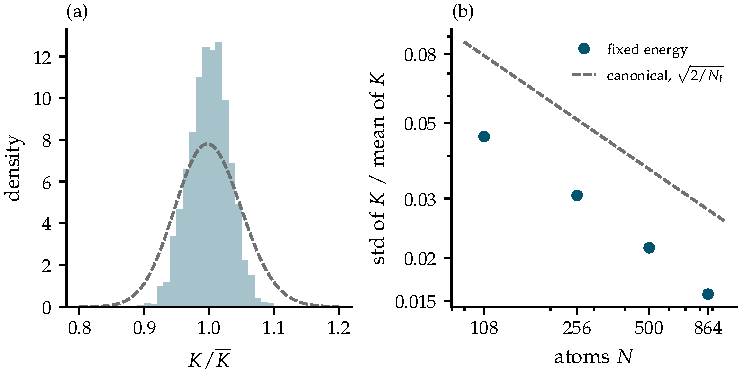
\includegraphics{ch12_ensembles/kinetic}
\caption{The kinetic energy at fixed total energy. (a) Liquid argon, 256
atoms over \SI{50}{\pico\second}: the histogram of the kinetic energy
divided by its mean, against the canonical density of
\cref{eq:sm-gamma} with $N_{\mathrm f} = 765$ and the same mean (dashed).
(b) The relative standard deviation of the kinetic energy for 108, 256,
500 and 864 atoms (circles), against the canonical $\sqrt{2/N_{\mathrm
f}}$ (dashed).}
\label{fig:sm-kinetic}
\end{figure}

\subsection*{The heat capacity, two ways}

\Cref{eq:sm-lpv} solved for $C_V$,
\begin{equation*}
   C_V = \frac{\frac12N_{\mathrm f}\kB}{1 - 2\ens{\delta K^2}_E/
   \bigl(N_{\mathrm f}(\kB T)^2\bigr)} ,
\end{equation*}
gives the heat capacity from one run at fixed energy;
\texttt{statmech.heat\_capacity\_nve} computes it, with $T$ the run's
kinetic temperature. \Cref{fig:sm-heat} checks it against the definition,
$C_V = \dd E/\dd T$. Five runs of the 256 atoms, prepared near 100, 115,
130, 145 and \SI{160}{\kelvin} and run for \SI{50}{\pico\second} each,
give five pairs of mean energy and mean kinetic temperature, from
\SI{99.25}{\kelvin} to \SI{160.28}{\kelvin}. They lie on a straight line
to within \SI{0.029}{\electronvolt}, whose slope is
\SI{0.05242}{\electronvolt\per\kelvin}, or $C_V = 2.376\,N\kB$. The
spreads of the five runs give between 2.249 and $2.444\,N\kB$, with the
mean 2.347, and the four sizes near \SI{130}{\kelvin} between 2.198 and
2.333. The liquid lies between an ideal gas, with $\frac32N\kB$ from its
kinetic energy alone, and a harmonic crystal, with $3N\kB$ from equal
kinetic and potential shares. The single-run estimates scatter about the
slope by up to 7.5\%; whether that scatter is the noise of runs of
\SI{50}{\pico\second} is a question Chapter~15 answers with error bars.
In the canonical ensemble the total energy itself fluctuates, and
\cref{eq:sm-fluctuation} gives $C_V$ directly, which Chapter~13 measures
under its thermostats.

\begin{figure}[htb]
\centering
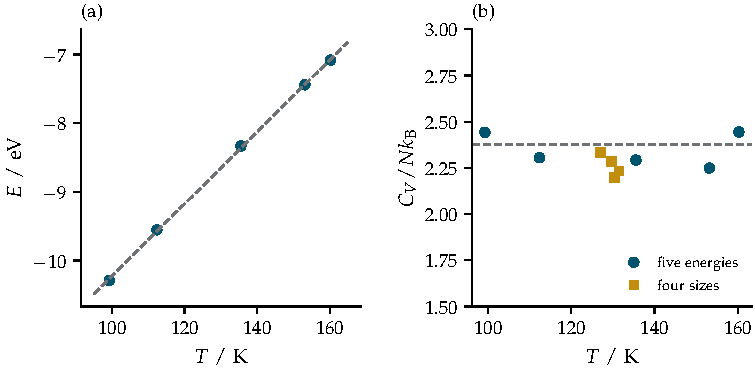
\includegraphics{ch12_ensembles/heat}
\caption{The heat capacity of liquid argon, 256 atoms. (a) The mean
energy against the mean kinetic temperature of five runs at fixed energy,
with the straight line through them, whose slope is $C_V$ (dashed).
(b) $C_V$ per atom, in units of $\kB$, from the spread of the kinetic
energy by \cref{eq:sm-lpv}, for the five runs (circles) and for runs of
108 to 864 atoms near \SI{130}{\kelvin} (squares), against the slope of
(a) (dashed).}
\label{fig:sm-heat}
\end{figure}

\begin{keyidea}
In the canonical ensemble the kinetic energy has the gamma distribution,
$\mathcal{P}(K) \propto K^{N_{\mathrm f}/2 - 1}\mathrm{e}^{-K/\kB T}$, with
mean $\frac12N_{\mathrm f}\kB T$ and relative spread
$\sqrt{2/N_{\mathrm f}}$. At fixed energy the kinetic and potential
energies share a fixed total, and the standard deviation of the kinetic
energy is $\sqrt{1 - N_{\mathrm f}\kB/(2C_V)}$ times the canonical one,
which gives the heat capacity from a single run.
\end{keyidea}

\notebook{12}{set the size and compare the kinetic energy at fixed energy with the canonical gamma distribution}

\begin{selfcheck}
By how much, relatively, does the kinetic temperature of 1000 atoms with
their drift removed fluctuate in the canonical ensemble?
\end{selfcheck}

%=============================================================================!
% 12.8  OTHER ENSEMBLES                                                       !
%=============================================================================!
\section{Other ensembles}
\label{sec:sm-other}

A sample on a bench exchanges more than energy with its surroundings: it
can swell against the air, and an electrode in a cell exchanges atoms and
electrons with the electrolyte and the circuit. This section extends the
argument of \cref{sec:sm-canonical} to a bath that also takes volume or
particles, finds the free energy each such ensemble makes least, and ends
with the electrons of an electronic-structure calculation.

\subsection*{Volume and particles}

The entropy of the bath depends on its volume and number of atoms as well
as its energy, and its slopes along them, each taken with the other two
held fixed (\cref{sec:ha-equations}), define the pressure $P$ and the
chemical potential $\mu$:
\begin{equation*}
   \frac{\partial S}{\partial E} = \frac1T , \qquad
   \frac{\partial S}{\partial V} = \frac PT , \qquad
   \frac{\partial S}{\partial N} = -\frac\mu T .
\end{equation*}
For the ideal gas of \cref{sec:sm-micro}, $\Omega \propto V^N$ gives
$\partial S/\partial V = N\kB/V$, so $PV = N\kB T$, the ideal gas law;
Chapter~14 shows that this $P$ is the force per unit area on the walls.
The minus sign makes $\mu$ the energy that one more atom brings, as $\dd
E$ below shows. As \cref{sec:sm-micro} showed for energy, two systems that
exchange volume settle where their values of $P/T$ agree, and two that
exchange atoms where their values of $\mu/T$ agree, once the atoms are
counted correctly. Swapping two atoms of one kind gives back the same
arrangement, so the $N!$ orderings of $N$ identical atoms are one
microstate, and $\Omega$ and $Z$ for $N$ such atoms are divided by $N!$, a
factor that changed nothing while $N$ was fixed. Without it the ideal gas,
with $\Omega \propto V^N$, gains $\ln V$ in $\ln\Omega$ for each atom
added whatever $N$ is, and two boxes sharing atoms would not settle at
equal densities, the larger box taking all the atoms;
with it, one more atom changes $\ln(V^N/N!)$ by $\ln V - \ln(N + 1)
\approx \ln(V/N)$, and two boxes at one temperature settle at equal
densities $N/V$.

A system that takes the volume $V_s$ from the bath as well as the energy
$E_s$ leaves the bath $\Omega_{\mathrm B}(E - E_s, V - V_s)$ microstates,
and the Taylor series of \cref{sec:sm-canonical}, now in two variables
with one term for each as in \cref{sec:en-gradient}, gives
\begin{equation*}
   \ln\Omega_{\mathrm B}(E - E_s, V - V_s) \approx \ln\Omega_{\mathrm B}(E, V)
   - \frac{E_s}{\kB T} - \frac{PV_s}{\kB T} ,
\end{equation*}
so a state of the system with energy $E_s$ and volume $V_s$ has the
probability proportional to $\mathrm{e}^{-\beta(E_s + PV_s)}$: the
isothermal-isobaric, or $NPT$, ensemble. A system that takes $N_s$ atoms
from the bath has, by the same steps with $\partial\ln\Omega_{\mathrm
B}/\partial N = -\mu/\kB T$,
\begin{equation*}
   \ln\Omega_{\mathrm B}(E - E_s, N - N_s) \approx \ln\Omega_{\mathrm B}(E, N)
   - \frac{E_s}{\kB T} + \frac{\mu N_s}{\kB T} ,
\end{equation*}
and so the weight $\mathrm{e}^{-\beta(E_s - \mu N_s)}$: the grand
canonical, or $\mu VT$, ensemble. Grouping the states by their volume or
their number of atoms, the sum over each group being a canonical partition
function, gives
\begin{equation*}
   Z_{NPT} = \int\mathrm{e}^{-\beta PV}Z(N, V, T)\,\dd V , \qquad
   \Xi = \sum_N\mathrm{e}^{\beta\mu N}Z(N, V, T) ,
\end{equation*}
and the derivatives of their logarithms give averages and fluctuations as
before: the volume of an $NPT$ run fluctuates with the variance $-\kB
T\,\dd\ens{V}/\dd P$ (\cref{ex:sm-volume}), large for a soft material and
small for a stiff one, which Chapter~14 uses to test a barostat's
coupling.

\subsection*{The free energies}

For a system in contact with a bath at $T$, the total energy is divided as
in \cref{sec:sm-micro}: when the system holds $E_s$ it has $\Omega(E_s)$
microstates and the entropy $S = \kB\ln\Omega(E_s)$, the bath has
$\Omega_{\mathrm B}(E - E_s)$, and the most probable division has the most
microstates of the two together, $\Omega(E_s)\,\Omega_{\mathrm B}(E -
E_s)$. Their logarithm times $\kB$ is the total entropy, which by the
expansion of \cref{sec:sm-canonical} is
\begin{equation*}
   S + S_{\mathrm B}(E - E_s) \approx S + S_{\mathrm B}(E)
   - \frac{E_s}{T} = S_{\mathrm B}(E) - \frac{E_s - TS}{T} .
\end{equation*}
$S_{\mathrm B}(E)$ is the same for every division, so the system settles
at the energy that makes $E_s - TS$ least, and for a large system that
least value is the free energy $F$ of \cref{sec:sm-canonical}. With a bath
that also takes volume, it is $F + PV$ that is least, the Gibbs free
energy, $-\kB T\ln Z_{NPT}$; with one that takes atoms, $F - \mu N$, the
grand potential, $-\kB T\ln\Xi$. From here on $E$, $V$ and $N$ are the
system's own.

For small changes $\dd E$, $\dd V$ and $\dd N$, the entropy changes by one
term for each, its slope times the change (\cref{sec:en-gradient}):
\begin{align*}
   \dd S &= \frac{\dd E}{T} + \frac{P\,\dd V}{T} - \frac{\mu\,\dd N}{T} ,\\
   \dd E &= T\,\dd S - P\,\dd V + \mu\,\dd N
   && \text{multiplying by $T$ and rearranging.}
\end{align*}
$TS$ changes by $T\,\dd S + S\,\dd T$, by the product rule, so
\begin{equation*}
   \dd F = \dd E - T\,\dd S - S\,\dd T = -S\,\dd T - P\,\dd V + \mu\,\dd N .
\end{equation*}
Since $T$ is the slope of $E$ along $S$, subtracting $TS$ exchanged $S$
for that slope as the variable the energy depends on. By
\cref{sec:ha-legendre}, $TS - E$ at the $S$ where the slope is $T$ is the
largest gap between the line $TS$ and the curve $E(S)$, the Legendre
transform of $E$; $F = E - TS$ is that transform with its sign reversed,
and so the least value of $E - TS$ over $S$, which is why the system
settles there. Adding $PV$ or subtracting $\mu N$ exchanges $V$ for $P$ or
$N$ for $\mu$ in the same way (\cref{ex:sm-legendre}).
\Cref{tab:sm-ensembles} collects the four ensembles and what samples each.

\begin{table}[htb]
\centering
\caption{The ensembles of this book: what is fixed, the probability of a
state, the quantity that is greatest or least, and what samples the
ensemble in a simulation.}
\label{tab:sm-ensembles}
\small
\begin{tabular}{@{}lllll@{}}
\toprule
ensemble & fixed & weight & extremum & sampled by\\
\midrule
microcanonical & $N$, $V$, $E$ & equal on the shell & $S$ largest &
   Verlet (Chs~9--11)\\
canonical & $N$, $V$, $T$ & $\mathrm{e}^{-\beta E}$ & $F$ least &
   thermostats (Ch.~13)\\
isothermal-isobaric & $N$, $P$, $T$ & $\mathrm{e}^{-\beta(E + PV)}$ &
   $F + PV$ least & barostats (Ch.~14)\\
grand canonical & $\mu$, $V$, $T$ & $\mathrm{e}^{-\beta(E - \mu N)}$ &
   $F - \mu N$ least & insertion and removal\\
\bottomrule
\end{tabular}
\end{table}

Molecular dynamics keeps the number of atoms, so the grand canonical
ensemble of atoms is sampled by moves that insert or remove an atom at
random and keep or undo each with a probability set by its weight, Monte
Carlo moves, which are not dynamics; this book does not use them. The
grand canonical ensemble returns for electrons.

\subsection*{Electrons in an orbital}

In an electronic-structure calculation the electrons of a solid fill
orbitals, states of definite energy $\varepsilon_{\mathrm o}$ that one electron can
occupy. No two electrons can be in the same state (the exclusion
principle), and an electron has a further two-valued property, its spin,
so an orbital holds either no electron of a given spin or one. In contact
with a reservoir of electrons at the chemical potential $\mu$, the orbital
with one spin is a system of two states: empty, with $N = 0$ and energy
0, and filled, with $N = 1$ and energy $\varepsilon_{\mathrm o}$. Its grand partition
function has two terms, $\Xi = 1 + \mathrm{e}^{-\beta(\varepsilon_{\mathrm o} -
\mu)}$, and its mean occupation, $0\times\mathcal{P}(\text{empty}) +
1\times\mathcal{P}(\text{filled})$, is the probability of the second,
\begin{align*}
   f &= \frac{\mathrm{e}^{-\beta(\varepsilon_{\mathrm o} - \mu)}}{1 +
   \mathrm{e}^{-\beta(\varepsilon_{\mathrm o} - \mu)}}\\
   &= \frac{1}{\mathrm{e}^{(\varepsilon_{\mathrm o} - \mu)/\kB T} + 1}
   && \text{dividing above and below by
   $\mathrm{e}^{-\beta(\varepsilon_{\mathrm o} - \mu)}$,}
\end{align*}
the Fermi-Dirac occupation: 0.5 at $\varepsilon_{\mathrm o} = \mu$, 0.0205 at
\SI{0.1}{\electronvolt} above it and 0.9795 at \SI{0.1}{\electronvolt}
below, at \SI{300}{\kelvin}. The entropy $-\kB\sum\mathcal{P}\ln\mathcal{P}$
of its two states, with probabilities $1 - f$ and $f$, is $-\kB[f\ln f +
(1 - f)\ln(1 - f)]$, whose slope in $f$, $\kB\ln\bigl((1 - f)/f\bigr)$,
vanishes at $f = \frac12$: the entropy is largest, $\kB\ln 2$, when the
orbital is half filled.

\begin{bridge}
Mermin showed that density functional theory carries over to a finite
temperature in the grand canonical ensemble, the grand potential of the
electrons being least at their true density\cite{Mermin1965}. A
calculation of a metal that smears its occupations with this $f$
minimises the free energy $E - TS$ of its electrons, with $S$ the sum of
the orbitals' entropies, and the force on each atom is the slope of that
free energy, so a run on such forces keeps constant the sum of the atoms'
kinetic energy and that free energy\cite{Wentzcovitch1992}, and not the
sum with $E$. A calculation of an electrode held at a fixed potential
fixes $\mu$ of the electrons instead of their number, and makes the grand
potential $E - TS - \mu N$ least: its electrons are in the grand
canonical ensemble, while its atoms may be canonical.
\end{bridge}

\begin{keyidea}
A bath that takes volume weights a state by $\mathrm{e}^{-\beta(E +
PV)}$, and one that takes atoms by $\mathrm{e}^{-\beta(E - \mu N)}$, with
identical atoms counted once, $N!$ orderings as one microstate. In
contact with a bath, the system makes a free energy least: $F = E - TS$ at
fixed $V$, $F + PV$ at fixed $P$, $F - \mu N$ at fixed $\mu$, each the
Legendre transform of the energy with its sign reversed. Fermi-Dirac
occupations are the grand canonical ensemble of one orbital.
\end{keyidea}

\notebook{12}{set a temperature and watch the occupations and their entropy}

\begin{selfcheck}
What is the occupation of an orbital $3\kB T$ below the chemical
potential?
\end{selfcheck}

%=============================================================================!
% 12.9  WHAT THE TRAJECTORY LOOKS LIKE                                        !
%=============================================================================!
\section{What the trajectory looks like}
\label{sec:sm-trajectory}

\Cref{sec:cs-trajectory} read a run through its energy, its bonds and its
centre of mass. This section reads it through its temperature and its
velocities: a healthy run of liquid argon first, then six faults that
show in them, each with the check that catches it.

\subsection*{A healthy run}

\Cref{fig:sm-healthy} follows the 256 atoms of liquid argon of
\cref{sec:sm-maxwell} for \SI{50}{\pico\second} at fixed energy. Its
kinetic temperature, over 765 freedoms, averages \SI{134.64}{\kelvin} over
every step (the frames saved every \SI{50}{\femto\second} give the
\SI{134.63}{\kelvin} of \cref{sec:sm-maxwell}), with
a standard deviation of \SI{4.13}{\kelvin}, 3.07\% of the mean, and stays
between 120.4 and \SI{147.8}{\kelvin}: a band with no trend, narrower than
the canonical 5.11\% of \cref{eq:sm-relative}, as \cref{eq:sm-lpv}
requires of a run at fixed energy. The total energy fluctuates by 0.0037
of the kinetic energy's spread, the check of \cref{sec:cs-trajectory}.
The temperatures of the three directions, each counting one component of
every velocity, have the running averages of \cref{fig:sm-healthy}(b),
which end at 132.80, 135.32 and \SI{134.20}{\kelvin}: the motion has no
preferred direction, as equipartition requires, to within 2\% after
\SI{50}{\pico\second}. Their mean, \SI{134.11}{\kelvin}, is $765/768$ of
the kinetic temperature, since each counts 256 components while the
removed drift takes one freedom from each direction
(\cref{sec:sm-equipartition}). The excess kurtosis of the velocities, computed on
each of 1001 frames of 768 components, has the mean $-0.010$ and the
standard deviation 0.190, and 4.2\% of the frames lie more than twice that
from zero, close to the 4.55\% beyond two standard deviations of a
Gaussian (\cref{sec:sm-probability}).

\begin{figure}[htb]
\centering
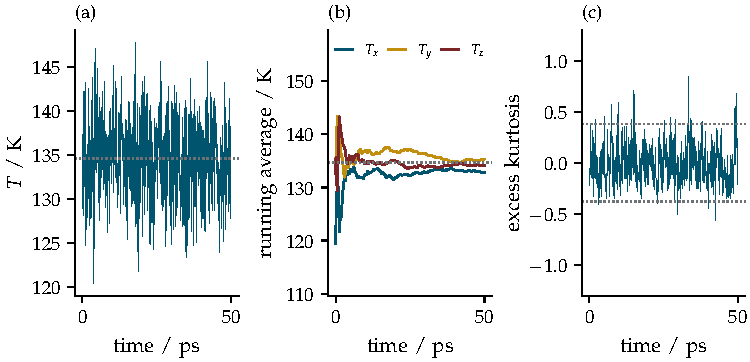
\includegraphics{ch12_ensembles/healthy}
\caption{A healthy run: 256 atoms of liquid argon at fixed energy for
\SI{50}{\pico\second}, steps of \SI{10}{\femto\second}. (a) The kinetic
temperature, with its mean (dotted). (b) The running averages of the
temperatures of the $x$, $y$ and $z$ components of the velocities. (c)
The excess kurtosis of the velocities every \SI{50}{\femto\second}, with
twice its standard deviation over the run either side of zero (dotted).}
\label{fig:sm-healthy}
\end{figure}

\subsection*{Six faults}

\Cref{fig:sm-faults} shows six faults and \cref{tab:sm-faults} the check
that catches each.

\begin{figure}[p]
\centering
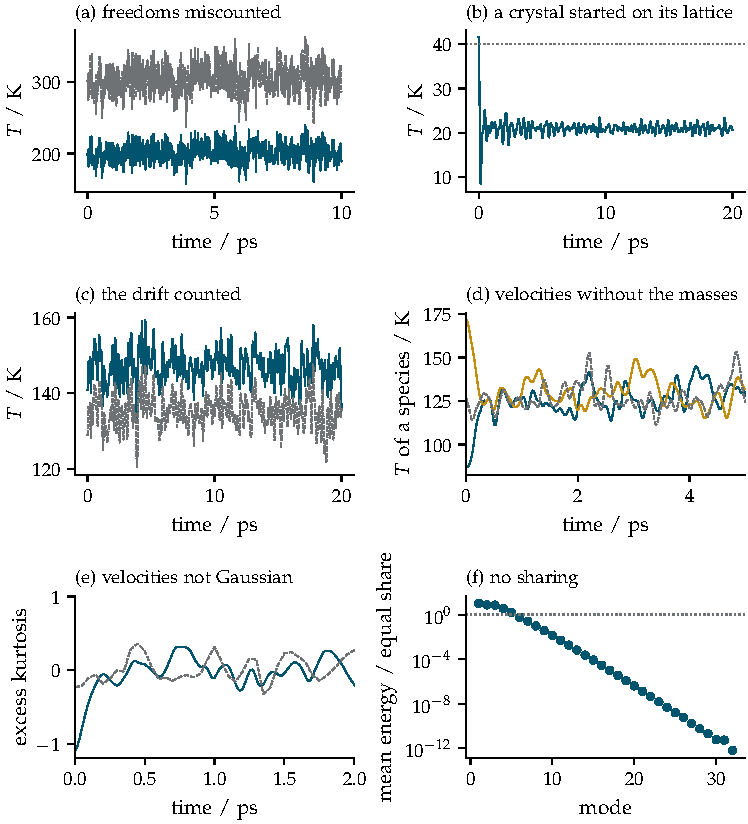
\includegraphics{ch12_ensembles/faults}
\caption{Faults that show in the temperature (teal), against the healthy
run (grey dashed). (a) The rigid water of Chapter~11 at
\SI{300}{\kelvin}, its kinetic energy divided among 381 freedoms (grey)
and among $3N = 576$ (teal). (b) 256 argon atoms started on their lattice
with velocities drawn at \SI{40}{\kelvin} (dotted). (c) The liquid
started with a drift of \SI{0.0005}{\angstrom\per\femto\second} in each
component of every velocity. (d) A liquid of atoms of two masses, 39.948
and \SI{83.798}{\amu}, started with one spread of velocity for all: the
temperatures of the light (teal) and heavy (ochre) atoms, against the
light atoms of the same liquid started with the masses (dashed). (e) The liquid started with
velocity components spread evenly over an interval: the excess kurtosis.
(f) The chain of \cref{fig:sm-ergodic}(a): the energy of each mode
averaged over 20\,000 units of time, divided by an equal share (dotted),
on a logarithmic axis.}
\label{fig:sm-faults}
\end{figure}

\begin{table}[htb]
\centering
\caption{The faults of \cref{fig:sm-faults}, the check that catches each,
and its value in the healthy run (for (f), under equal sharing) and in the
broken one.}
\label{tab:sm-faults}
\small
\begin{tabular}{@{}llll@{}}
\toprule
fault & check & healthy & broken\\
\midrule
(a) freedoms miscounted & $T$ against the value asked &
   \SI{303.9}{\kelvin} & \SI{201.0}{\kelvin}\\
(b) lattice start & mean $T$ over the last \SI{10}{\pico\second} / $T(0)$
   & 1.042 & 0.506\\
(c) drift counted & total momentum, amu\,\AA/fs &
   \num{1.5e-14} & 8.857\\
(d) masses ignored & $T$ of each species at the start &
   128, \SI{119}{\kelvin} & 88, \SI{171}{\kelvin}\\
(e) not Gaussian & \texttt{excess\_kurtosis} at the start & $-0.23$ &
   $-1.09$\\
(f) no sharing & share of modes 1 to 4 & 0.125 & 0.917\\
\bottomrule
\end{tabular}
\end{table}

\emph{(a) Freedoms miscounted.} The rigid water of \cref{sec:cs-water}
was prepared with \SI{12.93}{\milli\electronvolt} for each of its 381
freedoms, $\frac12\kB T$ at \SI{300}{\kelvin}, and over its
\SI{10}{\pico\second} run the kinetic temperature with that count averages
\SI{303.9}{\kelvin}. Divided among $3N = 576$, as if no distances were
held and no drift removed, the same kinetic energy reads
\SI{201.0}{\kelvin}, 0.661 of it, which is $381/576$. The run is sound
and only the reading is wrong. A thermostat that used the wrong count would
heat the water until the wrong reading came up to its target, here by a
factor of 1.51. The check is the kinetic energy per freedom against
$\frac12\kB T$, with the freedoms counted by
\texttt{degrees\_of\_freedom}.

\emph{(b) A crystal started on its lattice.} With velocities drawn at
\SI{40}{\kelvin}, the kinetic temperature at the start is
\SI{41.5}{\kelvin}; it falls below \SI{20}{\kelvin} within
\SI{0.1}{\pico\second}, reaches \SI{8.4}{\kelvin} at
\SI{160}{\femto\second}, and settles at \SI{21.0}{\kelvin}, 0.506 of
the start, as equipartition predicts for a nearly harmonic crystal
(\cref{sec:sm-equipartition}). The healthy liquid, prepared by several
rounds of redrawn velocities, rises by 4\% from its start. A run whose
temperature moves far from its start has not reached the state asked for,
and its early part is not yet the ensemble wanted; Chapter~15 finds where
such a run's averages can begin.

\emph{(c) The drift counted.} Starting velocities with a drift of
$v_{\mathrm d} = \SI{0.0005}{\angstrom\per\femto\second}$ in each component
move the whole box, of mass $M = 256\times39.948 = \SI{10227}{\amu}$, at
$\sqrt3\,v_{\mathrm d}$, with the kinetic energy $\frac12M\times
3v_{\mathrm d}^2\times103.6427 = \SI{0.397}{\electronvolt}$ and the
momentum $M\sqrt3\,v_{\mathrm d} = 8.857$\,amu\,\AA/fs, which momentum
conservation keeps for ever. Counted as heat over 765 freedoms it reads as
$2\times0.397/(765\kB) = \SI{12.1}{\kelvin}$: the run shows \SI{147.1}{\kelvin}, of which the motion
of the atoms relative to their centre of mass gives \SI{135.0}{\kelvin}.
The temperature looks healthy, a steady band; the check is the total
momentum, 8.857 against $\num{1.5e-14}$\,amu\,\AA/fs in the healthy run, or
\texttt{centre\_of\_mass\_path} of \cref{sec:cs-trajectory}. A thermostat
acting on the total kinetic energy would cool the relative motion to make
room for the drift; Chapter~13 meets the reverse, a thermostat that feeds
the drift, as the flying ice cube.

\emph{(d) Velocities drawn without the masses.} Drawing every atom's
components with one spread gives the light atoms of a mixture too little
kinetic energy and the heavy ones too much: \SI{88}{\kelvin} and
\SI{171}{\kelvin} at the start, against 128 and \SI{119}{\kelvin} when
the masses are used, values that scatter by $\sqrt{2/384} = 7\%$,
\cref{eq:sm-relative} for the 384 components of 128 atoms. Collisions share the energy out, and the gap between the
species first averages below \SI{15}{\kelvin} about \SI{260}{\femto\second}
in; over the last \SI{10}{\pico\second} the two species are at 130 and
\SI{128}{\kelvin}. In a liquid the fault costs only the first
picosecond. The check, \texttt{part\_temperature} for each species,
matters most where energy is shared slowly, as in (f).

\emph{(e) Velocities not Gaussian.} Components drawn evenly from an
interval, with the right mean square, have an excess kurtosis of $-1.09$ at
the start, near the $-1.2$ of an even spread, and the run reaches $-0.43$
after \SI{100}{\femto\second} and $-0.06$ after \SI{200}{\femto\second},
within the scatter of the healthy run. The temperature is right
throughout; only the shape of the distribution shows the fault, and in a
liquid it heals within a fraction of a picosecond. The fault is easy to
make: the forecasting code of TrajCast\cite{Thiemann2026}, asked to draw
starting velocities without naming a distribution, draws every component
evenly from one interval, the same for every mass, and rescales to the
temperature, faults (d) and (e) together. A kurtosis that stays away from
zero shows velocities that have not yet reached the Maxwell-Boltzmann
distribution.

\emph{(f) No sharing.} The chain of Fermi, Pasta, Ulam and Tsingou of
\cref{sec:sm-ergodic}, averaged over \num{20000} units of time, keeps 0.917
of its energy in its first four modes, against $4/32 = 0.125$ for equal
sharing; the first mode holds 10.7 times an equal share and no mode from
the eighth on holds more than 0.097 of one. Equipartition fails because
the trajectory does not explore its energy shell. The check, the energy of
each mode, or more generally the temperature of each part of a system,
detects a system that is not ergodic on the time scale of the run, which
no single average over the whole system reveals.

\begin{practice}
A run's temperature is read with the freedoms counted for that run, $3N -
n_{\mathrm c} - 3$ for a periodic run whose drift is removed, and compared
with the value asked for only after the early part has settled. The total
momentum should be zero, the temperatures of the three directions and of
each species should agree to the scatter of the run, and the excess
kurtosis of the velocities should be near zero. A run at
fixed energy has a kinetic temperature whose spread is below
$\sqrt{2/N_{\mathrm f}}$ of its mean; a run that claims to be canonical
must reach it, which is the first test of a thermostat in Chapter~13.
\end{practice}

\begin{keyidea}
A healthy run's kinetic temperature, counted over the right freedoms,
holds a steady band, with equal temperatures in each direction and for
each species and Gaussian velocities. Miscounted freedoms shift the
reading; a lattice start halves the temperature; a kept drift adds a
spurious steady part; velocities drawn without the masses or not Gaussian
heal in a liquid within a picosecond; a system that does not share its
energy keeps it in a few motions.
\end{keyidea}

\notebook{12}{break the liquid in each of the six ways and read the checks}

\begin{selfcheck}
A run of 500 argon atoms, drift removed, reports \SI{300}{\kelvin} from a
code that divides by $3N$. What temperature does the right count give?
\end{selfcheck}

%=============================================================================!
% 12.S  WHAT WE NOW HAVE                                                      !
%=============================================================================!
\unnumbered{What we now have}

A probability is the long-run fraction of trials with an outcome; a
continuous quantity has a density, the Gaussian chief among them, and
variances of independent quantities add. An ensemble is a cloud of copies
of a system in phase space, and the ergodic hypothesis equates its
averages with the time averages of one run: it is consistent with
liquid argon over \SI{50}{\pico\second} and fails for the harmonic chain. The chain of Fermi, Pasta, Ulam and
Tsingou has not shared its energy equally even after millions of units of
time; this is a finite-time limit on the averages we can obtain.

Counting the states of an isolated
system gives its entropy $S = \kB\ln\Omega$, and two systems sharing
energy settle where $\dd\ln\Omega/\dd E = 1/\kB T$ agrees. A system in
contact with a bath has the Boltzmann probabilities
$\mathrm{e}^{-E/\kB T}$, the partition function, the free energy $F =
-\kB T\ln Z$ and an energy variance $\kB T^2C_V$.

Each component of
velocity is Gaussian with variance $\kB T/m$, whatever the forces, and
every square term of the energy holds $\frac12\kB T$, so the kinetic
temperature $2K/(N_{\mathrm f}\kB)$ measures $T$ with $N_{\mathrm f} = 3N -
n_{\mathrm c} - 3$; \texttt{mdlab} and ASE agree once they count alike.

The kinetic energy has the gamma distribution with relative spread
$\sqrt{2/N_{\mathrm f}}$ in the canonical ensemble and less at fixed
energy, by an amount that gave the heat capacity of liquid argon,
$2.38\,N\kB$, from single runs to within 7.5\%.

Baths that take volume or
atoms give the $NPT$ and grand canonical ensembles, in which $F + PV$ and
$F - \mu N$ are least as $F$ is in the canonical one, each the energy's
Legendre transform with its sign reversed; Fermi-Dirac occupations are the
grand canonical ensemble of an orbital.

A healthy run
holds its kinetic temperature in a steady band, the same in every
direction and for every species, with Gaussian velocities; six faults
each leave their own mark.

Chapter~13 builds the thermostats that put a simulation in contact with a
bath, and tests each against the canonical distribution of the kinetic
energy derived here.

%=============================================================================!
% 12.A  ANSWERS TO THE CHECKS                                                 !
%=============================================================================!
\unnumbered{Answers to the checks}
\label{sec:sm-answers}

\answerto{sec:sm-probability}Totals of 10, 11 and 12 come from $3 + 2 + 1
= 6$ of the 36 outcomes: $6/36 = 1/6$.

\answerto{sec:sm-ergodic}$\omega_N = 2\sin(N\pi/(2N + 2))$, and $N\pi/(2N
+ 2)$ approaches $\pi/2$ as $N$ grows, so $\omega_N$ approaches 2 and the
period $2\pi/\omega_N$ approaches $\pi$; for $N = 32$ it is 3.145.

\answerto{sec:sm-micro}$1/\sqrt{120} = 0.0913$.

\answerto{sec:sm-canonical}$\kB T = \SI{0.008617}{\electronvolt}$ and
$\mathrm{e}^{-0.3/0.008617} = \num{7.6e-16}$.

\answerto{sec:sm-maxwell}$\sigma_v$ grows as $\sqrt T$:
$\sqrt2\times0.005995 = \SI{0.00848}{\angstrom\per\femto\second}$.

\answerto{sec:sm-equipartition}300 atoms and 300 held distances give
$N_{\mathrm f} = 900 - 300 - 3 = 597$, and $T = 2\times7.4/(597\kB) =
\SI{287.7}{\kelvin}$.

\answerto{sec:sm-kinetic}$N_{\mathrm f} = 2997$ and $\sqrt{2/2997} =
0.0258$, or 2.6\%.

\answerto{sec:sm-other}$f = 1/(\mathrm{e}^{-3} + 1) = 0.9526$.

\answerto{sec:sm-trajectory}The code divides by 1500 instead of 1497, so
the right count gives $300\times1500/1497 = \SI{300.6}{\kelvin}$.

%=============================================================================!
% 12.E  EXERCISES                                                             !
%=============================================================================!
\unnumbered{Exercises}
\label{sec:sm-exercises}

The exercises run from questions of understanding, through calculations,
to short derivations marked `show that'. Full solutions are in
\hyperref[sec:sm-solutions]{`Solutions to the exercises'} at the end of
the book, and Notebook~12 checks every numerical answer.

\begin{exercise}[a fair die]
\label{ex:sm-die}
Find the mean and the variance of the number shown by one fair die, and
the variance of the total of two.
\end{exercise}

\begin{exercise}[the spread of a mean]
\label{ex:sm-mean}
Show that the mean of $n$ independent values, each with the variance
$\sigma_x^2$, has the variance $\sigma_x^2/n$. How many throws of a die
make the standard deviation of their mean no more than 0.01?
\end{exercise}

\begin{exercise}[a chain of three]
\label{ex:sm-chain}
Find the angular frequencies of the three normal modes of a chain of
three atoms of unit mass between walls, joined by springs of unit
stiffness, from $\omega_k = 2\sin(k\pi/(2N + 2))$, and check that their
squares are the eigenvalues of the matrix with 2 on its diagonal, $-1$
just above and below it, and 0 elsewhere.
\end{exercise}

\begin{exercise}[entropies add]
\label{ex:sm-additive}
Show that two independent systems, with $\Omega_1$ and $\Omega_2$
microstates, have together the entropy $S_1 + S_2$.
\end{exercise}

\begin{exercise}[how large a bath]
\label{ex:sm-bath}
A system holding \SI{0.1}{\electronvolt} is in contact with a bath of
$10^4$ atoms of an ideal gas at \SI{300}{\kelvin}. What is the ratio of
the term of second order in the expansion of \cref{sec:sm-canonical} to
the term of first order, $E_s/\kB T$, which is kept?
\end{exercise}

\begin{exercise}[two levels]
\label{ex:sm-two-level}
A system has two states, of energies 0 and $E_{\mathrm g}$. Find $Z$,
$\ens{E}$ and $C_V$. For $E_{\mathrm g} = \SI{0.1}{\electronvolt}$, give
$\ens{E}$ and $C_V/\kB$ at \SI{300}{\kelvin}, and find numerically the
temperature at which $C_V$ is largest.
\end{exercise}

\begin{exercise}[free energy and entropy]
\label{ex:sm-free}
Show that $F = -\kB T\ln Z$ equals $\ens{E} - TS$ with $S =
-\kB\sum_s\mathcal{P}_s\ln\mathcal{P}_s$, and that this $S$ is $\kB\ln
\Omega$ when all $\Omega$ states are equally likely.
\end{exercise}

\begin{exercise}[a vibration's energy fluctuates]
\label{ex:sm-spring}
Show from the partition function $Z = 2\pi/(\beta\omega)$ of one
vibration that the variance of its energy is $(\kB T)^2$, and check
\cref{eq:sm-fluctuation} with $C_V = \kB$.
\end{exercise}

\begin{exercise}[odds and temperature]
\label{ex:sm-odds}
At what temperature are the odds of the \SI{0.3}{\electronvolt} barrier of
\cref{sec:sm-canonical} $10^{-3}$? What are the odds of a
\SI{0.5}{\electronvolt} barrier at \SI{300}{\kelvin}?
\end{exercise}

\begin{exercise}[speeds]
\label{ex:sm-speeds}
Show that the speed density of \cref{eq:sm-speed} is largest at
$\sqrt2\,\sigma_v$ and has the mean $\sqrt{8/\pi}\,\sigma_v$, and give
both for lithium at \SI{300}{\kelvin}.
\end{exercise}

\begin{exercise}[fourth moments]
\label{ex:sm-fourth}
Show that the Gaussian of mean zero has $\ens{x^4} = 3\sigma_x^4$, by
parts as in \cref{sec:sm-probability}, and that values spread evenly over
an interval $-c$ to $c$ have the excess kurtosis $-1.2$.
\end{exercise}

\begin{exercise}[light and heavy]
\label{ex:sm-species}
In a classical simulation of lithium-intercalated graphite at
\SI{300}{\kelvin}, find $\sigma_v$
for a lithium atom (\SI{6.94}{\amu}) and a carbon atom
(\SI{12.011}{\amu}), and their ratio. Which has the larger mean kinetic
energy?
\end{exercise}

\begin{exercise}[a turning molecule]
\label{ex:sm-rotor}
A molecule of two atoms with moment of inertia $I$ turns freely; its axis
points along the angles $\theta$ from $z$ and $\phi$ about $z$, and its
kinetic energy is $\frac12I(\dot\theta^2 + \sin^2\theta\,\dot\phi^2)$.
Show that $H = p_\theta^2/2I + p_\phi^2/(2I\sin^2\theta)$, and that its
mean is $\kB T$.
\end{exercise}

\begin{exercise}[counting freedoms]
\label{ex:sm-freedoms}
How many kinetic freedoms have (a) an isolated molecule of carbon
dioxide, a linear molecule of three atoms, with its drift and turning
removed; (b) 108 argon atoms in a periodic cell with the drift removed?
For (b), by what factor does ASE's temperature differ from
\texttt{mdlab}'s?
\end{exercise}

\begin{exercise}[how many atoms]
\label{ex:sm-scatter}
How many atoms, with the drift removed, does a canonical run need for its
kinetic temperature to have a standard deviation of 1\% of its mean?
\end{exercise}

\begin{exercise}[the most probable kinetic energy]
\label{ex:sm-mode}
Show that the gamma distribution of \cref{eq:sm-gamma} is largest at $K
= (\frac12N_{\mathrm f} - 1)\kB T$. Where is it largest for one atom,
and why is that not $\frac32\kB T$?
\end{exercise}

\begin{exercise}[a harmonic crystal at fixed energy]
\label{ex:sm-harmonic}
Show from \cref{eq:sm-lpv} that the kinetic energy of a harmonic
crystal at fixed energy fluctuates by $1/\sqrt2$ of the canonical amount.
\end{exercise}

\begin{exercise}[heat capacity from one run]
\label{ex:sm-heat}
A run of 500 atoms at fixed energy, drift removed, has a kinetic energy
whose standard deviation is 0.025 of its mean. Find $C_V$ per atom in
units of $\kB$.
\end{exercise}

\begin{exercise}[volume fluctuations]
\label{ex:sm-volume}
With the $NPT$ partition function
\begin{equation*}
   Z_{NPT} = \int\mathrm{e}^{-\beta PV}Z(N, V, T)\,\dd V ,
\end{equation*}
show that the mean volume is
\begin{equation*}
   \ens{V} = -\kB T\,\frac{\partial\ln Z_{NPT}}{\partial P}
\end{equation*}
and that its variance is $-\kB T\,\dd\ens{V}/\dd P$.
\end{exercise}

\begin{exercise}[the other potentials]
\label{ex:sm-legendre}
From $\dd E = T\,\dd S - P\,\dd V + \mu\,\dd N$, show that $F + PV$ changes
by $-S\,\dd T + V\,\dd P + \mu\,\dd N$ and $F - \mu N$ by $-S\,\dd T -
P\,\dd V - N\,\dd\mu$.
\end{exercise}

\begin{exercise}[Fermi-Dirac]
\label{ex:sm-fermi}
Show that the Fermi-Dirac occupation satisfies $f(\mu + x) = 1 - f(\mu -
x)$ and has the slope $-1/(4\kB T)$ at $\varepsilon_{\mathrm o} = \mu$. Find the
entropy, in units of $\kB$, of an orbital \SI{0.1}{\electronvolt} above
$\mu$ at \SI{300}{\kelvin}.
\end{exercise}

\begin{exercise}[a diagnosis]
\label{ex:sm-diagnose}
A long run of argon at fixed energy reports steady direction
temperatures $T_x = T_y = \SI{295}{\kelvin}$ and $T_z =
\SI{310}{\kelvin}$, each counting one component of every velocity. What
fault does this suggest, which check confirms it, and what velocity of
the centre of mass along $z$ would account for the difference?
\end{exercise}


%=============================================================================!
% CHAPTER 13  THERMOSTATS                                                     !
%=============================================================================!
\chapter{Thermostats}
\label{ch:thermostats}

%=============================================================================!
% 13.0  CHAPTER OPENING                                                       !
%=============================================================================!
Chapter~12 described the canonical distribution of a system in contact
with a heat bath. To reproduce that situation in a simulation, an
algorithm must exchange energy with the atoms while preserving the
required distribution. Such an algorithm is called a thermostat. We
judge it by two questions: whether it samples the canonical ensemble,
and how much it changes the motion during sampling.

We develop six approaches, beginning with direct velocity rescaling and
ending with the stochastic rescaling used by TrajCast. Comparisons on
liquid argon and on lithium atoms moving over the model surface of
Chapter~3 show why a suitable method depends on the measurement. The
chapter draws together choices for equilibration, equilibrium averages
and dynamics, then examines the signs of faulty thermostatting in a
trajectory. Chapter~14 applies the same distinction between mean values,
fluctuations and motion to pressure control.

%=============================================================================!
% 13.1  WHAT A THERMOSTAT MUST DO                                             !
%=============================================================================!
\section{What a thermostat must do}
\label{sec:th-tests}

A real sample keeps its temperature by exchanging energy with what
surrounds it, which a simulation leaves out. A thermostat stands in for
those surroundings. This section sets out what it must achieve, what it
should leave alone, how the chapter tests both, and the single loop into
which every thermostat of the chapter fits.

\subsection*{Two demands}

The first demand is the canonical ensemble of \cref{sec:sm-canonical}. A
run's time averages should equal averages with the weight
$\mathrm{e}^{-\beta H}$, which means three things that can be checked:
the kinetic energy of the $N_{\mathrm f}$ freedoms has the gamma
distribution of \cref{eq:sm-gamma}, with the relative spread
$\sqrt{2/N_{\mathrm f}}$; the positions have the density
$\mathrm{e}^{-\beta U}$ (\cref{sec:sm-canonical}); and the velocities are
Maxwellian and independent of the positions (\cref{sec:sm-maxwell}).
A thermostat that holds the mean temperature but narrows the spread of $K$
samples the wrong ensemble, and every quantity drawn from its
fluctuations, such as the heat capacity of \cref{eq:sm-fluctuation}, is
wrong.

The second demand is softer: the motion should stay close to the motion
of the real system. In a sample the surroundings exchange energy only at
its edges and only slowly, and the atoms inside move by Newton's laws. A
thermostat acts on every atom at every step, so it changes the motion
everywhere, and how much it changes it decides whether a diffusion
coefficient, a rate of hopping or a vibrational frequency measured under
it means anything. The two demands can pull apart: a thermostat that
acts on each atom separately, as those of \cref{sec:th-andersen,sec:th-langevin}
do, disturbs the motion more the more firmly it holds the temperature.

\subsection*{The tests}

Every thermostat in the chapter is tested on two systems. The first is
the liquid argon of Chapter~12, 256 atoms at \SI{135}{\kelvin}, started
from three frames of the run of \cref{sec:sm-ergodic} 20 picoseconds
apart and followed for \SI{100}{\pico\second} with steps of
\SI{10}{\femto\second}, the first \SI{5}{\pico\second} of each set aside
for the distribution of $K$; the three runs give each measured quantity a
mean and a spread. On it we measure the distribution of $K$; the
diffusion coefficient $D$, which measures how fast atoms wander: the
square of the distance an atom moves in a time $t$, averaged over the
atoms and the starting times, grows in proportion to $t$ in a liquid, and
$D$ is a sixth of its slope between 2 and \SI{20}{\pico\second}, with
positions measured from the centre of mass (Chapter~16 treats this
properly, the six included); and the cost, the computing time of a step
against that of velocity Verlet alone.

The second is lithium on the model surface of \cref{sec:en-surface},
standing for lithium in graphite: 1000 atoms, each on its own copy of the
surface with its own thermostat, at \SI{1000}{\kelvin}, started from the
density $\mathrm{e}^{-\beta U}$ and the Maxwell-Boltzmann distribution.
The temperature is high so that hops are frequent: the estimate of
\cref{sec:th-langevin} puts one hop every \SI{1.69}{\nano\second} at
\SI{300}{\kelvin} and \SI{1.26}{\per\pico\second} at \SI{1000}{\kelvin}.
Each atom has only two freedoms, the hardest case for a thermostat: its
kinetic energy should spread as widely as \cref{eq:sm-gamma} with
$N_{\mathrm f} = 2$, a relative spread of 1, and it has no other atoms to
share energy with. Its
exact canonical density of positions is known, so the distribution of
its potential energy can be compared with the exact one, computed on a
grid over one cell of the surface; and its hops can be counted.

\subsection*{The heat and the effective energy}

A thermostat adds or removes kinetic energy at each step. Adding up what
it adds over a run gives the heat it has put in, and the effective energy
\begin{equation}
   E_{\mathrm{eff}} = K + U - \text{heat}
   \label{eq:th-effective}
\end{equation}
counts every change of $K + U$ that the thermostat did not make. Between
the thermostat's actions the motion is Newton's, which keeps $K + U$, so
in exact dynamics $E_{\mathrm{eff}}$ never changes, for every thermostat.
In a run it drifts only through the error of the integrator, and that
drift is the thermostatted counterpart of the energy check of
\cref{sec:cs-trajectory}.

\subsection*{One loop for every thermostat}

Velocity Verlet (\cref{eq:in-kdk}) is a half kick, a drift and a half
kick. Splitting the drift into two halves, as \cref{sec:in-splitting}
split the Liouville operator, gives four pieces, B A A B, with B a half
kick and A a half drift. A thermostat may act before the step, between the
two half drifts, or after the step (\cref{fig:th-step}).
\texttt{mdlab.thermostats.run} is that loop:

\begin{code}
    for step in range(n_steps + 1):
        if step > 0:
            v = act(th.before, v)
            v = v + 0.5 * dt * accel * f
            r = r + 0.5 * dt * v
            v = act(th.middle, v)
            r = r + 0.5 * dt * v
            u, f = model(r)
            v = v + 0.5 * dt * accel * f
            v = act(th.after, v)
\end{code}

\noindent The pass with \texttt{step} 0 makes no step; it and every later
pass end by recording the state, which the listing leaves out.
\texttt{accel} is \texttt{FORCE\_TO\_ACCEL} divided by each mass, and \texttt{act} calls the thermostat's method and adds the change
of kinetic energy it makes to the heat. With no thermostat the three
calls do nothing and the loop is velocity Verlet; the thermostats of the
next sections each fill one or two of the calls. ASE implements five of
them independently. For four, Berendsen's, Langevin's, the Nosé-Hoover
chain and CSVR, from the same start of 32 argon atoms, with the same
random numbers for the two that use them, the two codes agree after 50
steps of \SI{5}{\femto\second} to within \SI{1e-7}{\angstrom} in every
position. ASE's version of Andersen's draws its random numbers
differently, so the two are compared by what they sample: over four runs
of \SI{100}{\pico\second} of the same atoms at \SI{120}{\kelvin}, the
mean kinetic temperature is $(119.40 \pm 0.55)$\,\si{\kelvin} under ASE's
and $(119.95 \pm 0.37)$\,\si{\kelvin} under \texttt{mdlab}'s, each with
0.99 to 1.01 of the canonical spread.

\begin{figure}[htb]
\centering
\begin{tikzpicture}[line cap=round, line join=round,
   box/.style={draw, line width=0.6pt, minimum width=0.9cm,
               minimum height=0.6cm, font=\small},
   th/.style={draw, line width=0.6pt, fill=accent!12, minimum width=1.2cm,
              minimum height=0.6cm, font=\scriptsize, align=center}]
   \node[th] (b0) at (0,0) {before};
   \node[box] (k1) at (1.45,0) {B};
   \node[box] (d1) at (2.6,0) {A};
   \node[th] (mid) at (3.9,0) {middle};
   \node[box] (d2) at (5.2,0) {A};
   \node[box] (k2) at (6.35,0) {B};
   \node[th] (a0) at (7.8,0) {after};
   \foreach \x/\y in {b0/k1, k1/d1, d1/mid, mid/d2, d2/k2, k2/a0}
      \draw[-{Stealth[length=4pt]}, line width=0.5pt] (\x) -- (\y);
   \node[font=\scriptsize, align=center, anchor=north] at (0,-0.5)
      {rescaling\\Berendsen\\CSVR\\chains, $\tfrac12$};
   \node[font=\scriptsize, align=center, anchor=north] at (3.9,-0.5)
      {Langevin};
   \node[font=\scriptsize, align=center, anchor=north] at (7.8,-0.5)
      {Andersen\\chains, $\tfrac12$};
\end{tikzpicture}
\caption{One step of \texttt{mdlab.thermostats.run}: velocity Verlet as a
half kick (B), two half drifts (A) and a half kick, with the places where
each thermostat of the chapter acts; Nosé-Hoover chains act for half a
step before and half after.}
\label{fig:th-step}
\end{figure}

\begin{keyidea}
A thermostat must give the canonical distributions, the gamma
distribution of $K$ with spread $\sqrt{2/N_{\mathrm f}}$ and the density
$\mathrm{e}^{-\beta U}$ of positions, and should disturb the motion as
little as it can. The effective energy, $K + U$ less the heat the
thermostat has added, is kept by the exact dynamics of every thermostat,
and its drift measures the integration error.
\end{keyidea}

\begin{selfcheck}
A thermostat removes \SI{0.5}{\electronvolt} over a run in which $K + U$
falls by \SI{0.48}{\electronvolt}. By how much has the effective energy
changed?
\end{selfcheck}

%=============================================================================!
% 13.2  RESCALING AND WEAK COUPLING                                           !
%=============================================================================!
\section{Rescaling and weak coupling}
\label{sec:th-berendsen}

The simplest way to hold a temperature is to multiply every velocity by
the factor that brings the kinetic energy to its target. This section
builds that, and the gentler version of Berendsen and his colleagues,
measures what both do to the distribution of $K$, and derives two faults
they share.

\subsection*{Rescaling}

Before each step, \texttt{Rescale} multiplies every velocity by
$\lambda = \sqrt{K_0/K}$, with $K_0 = \frac12N_{\mathrm f}\kB T_0$ the
kinetic energy of the target temperature $T_0$; multiplying every
velocity by $\lambda$ multiplies $K$ by $\lambda^2$. The kinetic energy is
then exactly $K_0$ at the start of every step, and the only fluctuation
left is what the motion produces within one step: over \SI{95}{\pico
\second} of liquid argon, recorded at the ends of the steps, the relative
spread of $K$ is 0.0056, against the canonical 0.0511. The canonical
ensemble has a spread; rescaling all but removes it, and with it any use
of the fluctuation formulae of \cref{sec:sm-kinetic}. The scaling factor $\lambda$ is a
symbol of this chapter only (\cref{sec:la-multipliers,sec:cs-shake} used
it for a multiplier).

\subsection*{Weak coupling}

Berendsen and colleagues asked the temperature instead to relax towards
$T_0$ with a time constant $\tau_{\mathrm T}$\cite{Berendsen1984},
\begin{equation*}
   \frac{\dd T}{\dd t} = \frac{T_0 - T}{\tau_{\mathrm T}} .
\end{equation*}
Here $T$ is the kinetic temperature $T_{\mathrm{kin}}$ of Chapter~12.
Over one step $\dt$ the kinetic temperature should change by $(\dt/
\tau_{\mathrm T})(T_0 - T)$. Scaling the velocities by $\lambda$ turns $T$
into $\lambda^2T$, so
\begin{equation}
   \lambda^2T = T + \frac{\dt}{\tau_{\mathrm T}}(T_0 - T) , \qquad
   \lambda^2 = 1 + \frac{\dt}{\tau_{\mathrm T}}\Bigl(\frac{T_0}{T} - 1
   \Bigr) .
   \label{eq:th-berendsen}
\end{equation}
At \SI{150}{\kelvin}, with a target of \SI{135}{\kelvin}, steps of
\SI{10}{\femto\second} and $\tau_{\mathrm T} = \SI{100}{\femto\second}$,
$\lambda^2 = 0.9900$ and $\lambda = 0.99499$: the velocities shrink by half
a percent. With $\tau_{\mathrm T} = \dt$ this is rescaling; as
$\tau_{\mathrm T}$ grows, the run approaches one at fixed energy.

One thing follows from \cref{eq:th-berendsen}. The scaling turns $K$ into
$\lambda^2K$, so each step adds the heat $(\lambda^2 - 1)K =
(\dt/\tau_{\mathrm T})(K_0 - K)$, since $T_0K/T = K_0$. Over a long run in
which nothing drifts this heat averages to zero, because by
\cref{eq:th-effective} the total heat is the change of $K + U$, which stays
within its fluctuations however long the run; so $\ens{K} = K_0$ and the
mean temperature is exactly the target. Over three runs it is \SI{135.00}{\kelvin} with
$\tau_{\mathrm T} = \SI{100}{\femto\second}$ and \SI{135.02}{\kelvin}
with \SI{1}{\pico\second}. But the spread of $K$ is not the canonical
one (\cref{fig:th-berendsen}(a)): with $\tau_{\mathrm T} =
\SI{100}{\femto\second}$ it is 0.0228, 0.45 of the canonical spread and
smaller even than the 0.0311 of a run at fixed energy; with
\SI{1}{\pico\second}, 0.0300, close to the run at fixed energy. Berendsen
coupling does not sample the canonical ensemble at any $\tau_{\mathrm T}$:
strong coupling squeezes the fluctuations, and weak coupling leaves them
those of fixed energy.

\begin{figure}[htb]
\centering
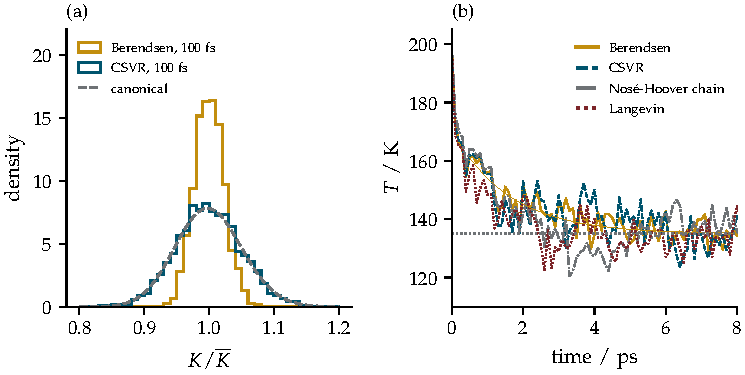
\includegraphics{ch13_thermostats/berendsen}
\caption{(a) The kinetic energy of liquid argon, divided by its mean,
over three runs of \SI{95}{\pico\second} under Berendsen and under CSVR
(\cref{sec:th-csvr}), both with $\tau_{\mathrm T} =
\SI{100}{\femto\second}$, against the canonical gamma density of 765
freedoms (dashed). (b) The liquid with its velocities scaled to
\SI{200}{\kelvin}, brought towards \SI{135}{\kelvin} by Berendsen
and CSVR with $\tau_{\mathrm T} = \SI{1}{\pico\second}$, a Nosé-Hoover
chain with $\tau_{\mathrm T} = \SI{1}{\pico\second}$
(\cref{sec:th-nose}) and Langevin with $\gamma = \SI{1}{\per\pico\second}$
(\cref{sec:th-langevin}), against the approach predicted for Berendsen
(thin). The target is the dotted line.}
\label{fig:th-berendsen}
\end{figure}

\subsection*{What the time constant means}

The temperature takes longer than $\tau_{\mathrm T}$ to settle.
\Cref{fig:th-berendsen}(b) starts the liquid at \SI{200}{\kelvin} by
scaling its velocities. Within \SI{0.2}{\pico\second} the kinetic
temperature falls to between 165 and \SI{170}{\kelvin} under every
thermostat, as kinetic energy passes into potential energy, the sharing
of \cref{sec:sm-equipartition}. After that the thermostat removes heat at
the rate $(K - K_0)/\tau_{\mathrm T} = C_K(T - T_0)/\tau_{\mathrm T}$,
with $C_K = \frac12N_{\mathrm f}\kB$ the kinetic part of the heat
capacity (\cref{sec:sm-kinetic}). But the liquid's energy exceeds its
value at $T_0$ by $C_V(T - T_0)$, more than the $C_K(T - T_0)$ held as
kinetic energy, so it
changes at the rate $C_V\,\dd T/\dd t$, and equating the two,
\begin{equation*}
   C_V\frac{\dd T}{\dd t} = -\frac{C_K}{\tau_{\mathrm T}}(T - T_0) ,
\end{equation*}
and $T - T_0$ decays as $\mathrm{e}^{-t/\tau_{\mathrm{eff}}}$, as the gap
$w$ of \cref{sec:ne-drag} did, with $\tau_{\mathrm{eff}} = \tau_{\mathrm
T}C_V/C_K$. With $C_V = 2.376\,N\kB$ and $C_K = 1.4941\,N\kB$ from
\cref{sec:sm-kinetic}, $C_V/C_K = 1.590$, so $\tau_{\mathrm{eff}} =
\SI{1.59}{\pico\second}$ for $\tau_{\mathrm T} = \SI{1}{\pico\second}$; a
fit to the run from \SI{0.5}{\pico\second} on gives
\SI{1.67}{\pico\second}, uncertain by \SI{0.19}{\pico\second} in a single
run.

\subsection*{The flying ice cube}

Rescaling and Berendsen coupling multiply every velocity by the same
factor, including the part of each velocity that belongs to the motion of
the whole box. No force changes that motion (\cref{sec:ne-atoms}), so its
kinetic energy $K_{\mathrm{com}}$ changes only by the thermostat, by the
factor $\lambda^2$ at each step. Over $n$ steps, $\ln K_{\mathrm{com}}$
gains $\sum\ln\lambda^2$. Writing $T = T_0 + \delta T$, whose departure
$\delta T$ from the target has mean zero since $\ens{T} = T_0$,
\begin{align*}
   \lambda^2 - 1 &= \frac{\dt}{\tau_{\mathrm T}}\Bigl(\frac{1}{1 + \delta
   T/T_0} - 1\Bigr) = \frac{\dt}{\tau_{\mathrm T}}\Bigl(-\frac{\delta T}{T_0}
   + \Bigl(\frac{\delta T}{T_0}\Bigr)^2 - \dotsb\Bigr) ,\\
   \ens{\ln\lambda^2} &\approx \ens{\lambda^2 - 1}
   \approx \frac{\dt}{\tau_{\mathrm T}}\Bigl\langle\Bigl(\frac{\delta
   T}{T_0}\Bigr)^2\Bigr\rangle ,
\end{align*}
to first order in $\dt/\tau_{\mathrm T}$ and second in $\delta T/T_0$,
using $1/(1 + y) = 1 - y + y^2 - \dotsb$, which holds because $(1 + y)(1 -
y + y^2) = 1 + y^3$, and $\ln(1 + y) \approx y$ for small $y$, the Taylor
series of \cref{sec:mo-taylor} with the slope $1/(1 + y)$ of the
logarithm, 1 at $y = 0$. The mean is positive whatever the sign of the
fluctuations, and over $n$ steps, a time $t = n\dt$, $\ln K_{\mathrm{com}}$
gains $n\ens{\ln\lambda^2} \approx \ens{(\delta T/T_0)^2}t/\tau_{\mathrm
T}$: $K_{\mathrm{com}}$ grows as $\mathrm{e}^{\ens{(\delta
T/T_0)^2}t/\tau_{\mathrm T}}$, at
the expense of the motion of the atoms against one another, which the
thermostat cools to keep the total at $K_0$. In time the box flies
through space while its atoms freeze, the flying ice cube of Harvey, Tan
and Cheatham, who found velocity rescaling to break the equipartition of
energy\cite{Harvey1998}, revisited by Braun, Moosavi and
Smit\cite{Braun2018}.
For liquid argon with $\tau_{\mathrm T} = \SI{100}{\femto\second}$,
$\ens{(\delta T/T_0)^2} = \num{4.99e-4}$ in the first of the three runs, and the
predicted rate is \SI{0.0050}{\per\pico\second}; keeping the next term of
$\ln(1 + y)$, $-\frac12y^2$, lowers it by the factor $1 - \dt/2\tau_{\mathrm
T} = 0.95$, to \SI{0.0047}{\per\pico\second}, which
\cref{sec:th-trajectory} measures. A weaker form of the same flow feeds
any motion that the forces barely touch, such as the slow vibrations of
large molecules, held back only by its slow exchange of energy with the
other motions, which is why the effect appears even when the motion of
the centre of mass has been removed\cite{Harvey1998,Braun2018}. For one lithium atom on the surface, whose two freedoms are
its whole motion, Berendsen coupling with $\tau_{\mathrm T} =
\SI{100}{\femto\second}$ drives the atom within a picosecond or two onto
a circular orbit of radius \SI{0.48}{\angstrom} round its hollow, on which
$K$ stays at $\kB T_0$ and $K + U$ at \SI{0.19}{\electronvolt}, short of
the \SI{0.3}{\electronvolt} barrier, and the thermostat has nothing left to
correct: the 1000 atoms make 0.001 hops per atom per picosecond, against
0.93 to 1.09 under the thermostats that sample correctly.

\begin{practice}
Rescaling and Berendsen coupling are for bringing a system near a
temperature quickly. Their averages of $T$ are right, but their
fluctuations are not, and a long run under them feeds slow motions and
the motion of the centre of mass. A production run, whose fluctuations or slow motions matter,
uses one of the thermostats of the next sections.
\end{practice}

\begin{keyidea}
Berendsen coupling scales the velocities by the factor $\lambda$ of
\cref{eq:th-berendsen}, so that $T$ relaxes towards $T_0$.
It holds the mean temperature exactly but narrows the spread of $K$
below the canonical one, and it feeds motions that the forces do not
touch, at the rate $\ens{(\delta T/T_0)^2}/\tau_{\mathrm T}$: the flying
ice cube. The
temperature of a liquid relaxes with the time constant $\tau_{\mathrm T}
C_V/C_K$, longer than $\tau_{\mathrm T}$.
\end{keyidea}

\notebook{13}{set the coupling time and watch the spread of K and the drift}

\begin{selfcheck}
What is $\lambda$ for a step of \SI{2}{\femto\second} with $\tau_{\mathrm
T} = \SI{1}{\pico\second}$, at \SI{310}{\kelvin} with a target of
\SI{300}{\kelvin}?
\end{selfcheck}

%=============================================================================!
% 13.3  COLLISIONS WITH A BATH                                                !
%=============================================================================!
\section{Collisions with a bath}
\label{sec:th-andersen}

A gas held at a temperature by the walls of its container gains its
temperature in collisions: an atom that strikes the wall leaves it with a
velocity typical of the wall's temperature. Andersen built a thermostat
on that picture\cite{Andersen1980}. This section shows why it samples the
canonical ensemble and measures what it does to the motion.

\subsection*{The method}

Each atom collides with an imagined bath at the rate $\nu$, and a
collision replaces its velocity with one drawn afresh from the
Maxwell-Boltzmann distribution at $T_0$, by \cref{eq:sm-maxwell}.
Collisions at the rate $\nu$, each independent of the last, leave an atom
untouched over a step with the probability $\mathrm{e}^{-\nu\dt}$
(\cref{ex:th-collisions}), so after each step \texttt{Andersen} redraws
the velocity of each atom with the probability $1 - \mathrm{e}^{-\nu\dt}$.
ASE's version redraws single components instead of whole velocities,
after the first half kick instead of after the step, and by default
removes the motion of the centre of mass; its redraws keep the same
distribution, and \cref{sec:th-tests} compares the two.

\subsection*{Why it is canonical}

The canonical density $\mathrm{e}^{-\beta H}/Z$ is kept by both parts of
the motion. Between collisions the atoms follow Hamilton's equations,
which keep every density that depends on the state only through $H$
(\cref{sec:ha-liouville}). In a collision one atom's velocity is replaced;
in the canonical density that velocity is independent of every other
coordinate and momentum and has the Maxwell-Boltzmann distribution
(\cref{sec:sm-maxwell}), so replacing it with a fresh, independent draw
from the same distribution leaves the joint density as it was. A density
that neither part changes does not change at all: the canonical ensemble
is stationary under Andersen's thermostat, and the collisions, which move
the run from one energy to another, carry it through the
ensemble\cite{Andersen1980}.

\subsection*{What it does to the motion}

A collision forgets the atom's velocity, so a thermostat that collides
often erases the momentum by which atoms push through a liquid. Over three
runs each, the diffusion coefficient of liquid argon is $0.96$, $0.72$ and
$0.17$ of its value at fixed energy, $(3.81 \pm 0.08)\times10^{-4}$\,\AA$^2$/fs,
for $\nu = 0.1$, 1 and \SI{10}{\per\pico\second}
(\cref{fig:th-coupling}(a) of \cref{sec:th-langevin}, with Langevin's
friction). At the weakest coupling the motion is barely disturbed, but
the temperature is held loosely: each atom collides once in
\SI{10}{\pico\second}, the three runs average 133.66, 130.13 and
\SI{131.69}{\kelvin} over their last \SI{95}{\pico\second}, counting all
$3N = 768$ freedoms since the collisions move the centre of mass too, and
the spread of $K$ within them is 0.85 of the canonical spread. At $\nu =
\SI{1}{\per\pico\second}$ the spread is 0.98 of it and the mean
$(134.5 \pm 0.6)$\,\si{\kelvin}. Collisions also change the total momentum, so
the box as a whole wanders, which \cref{sec:th-trajectory} shows to
matter when displacements are measured. For one lithium atom on the
surface, with $\nu = \SI{1}{\per\pico\second}$, the density of its
potential energy matches the exact one to within 0.011 of its peak.

\begin{keyidea}
Andersen's thermostat redraws each atom's velocity from the
Maxwell-Boltzmann distribution at the rate $\nu$. Hamilton's equations
and the redraws both keep the canonical density, and the redraws carry a
run from one energy to another, so the thermostat samples it, even for a
single atom. The redraws erase momentum: the
diffusion coefficient of liquid argon falls to 0.72 of its value at
$\nu = \SI{1}{\per\pico\second}$ and to 0.17 at
\SI{10}{\per\pico\second}, while weak coupling holds the temperature
only loosely.
\end{keyidea}

\begin{selfcheck}
With $\nu = \SI{1}{\per\pico\second}$ and steps of
\SI{2}{\femto\second}, what fraction of atoms is redrawn at each step, and
how many atoms of 1000 on average?
\end{selfcheck}

%=============================================================================!
% 13.4  FRICTION AND NOISE                                                    !
%=============================================================================!
\section{Friction and noise}
\label{sec:th-langevin}

A grain of pollen in water is struck by molecules from every side; on
average the blows slow it down, a friction, and their irregularity jostles
it, a noise. Langevin's equation keeps both and nothing else of the
water. This section solves the equation for one velocity, finds the
relation between friction and noise that gives the canonical
distribution, builds the BAOAB step from it, and measures how the
friction changes diffusion and the rate of hopping.

\subsection*{Random kicks}

\begin{toolbox}[A sum of random kicks]
A velocity that receives, at each of many short intervals of length $h$,
a kick $\sigma\sqrt h\,g$, with $g$ a fresh number from the normal
distribution of mean 0 and variance 1, has after $n$ kicks the variance
$n\sigma^2h = \sigma^2t$, with $t = nh$. Each kick has the variance
$\sigma^2h$, since multiplying a quantity by a constant multiplies every
deviation from its mean by that constant, and so its variance by the
constant's square; and variances of independent kicks add
(\cref{sec:sm-probability}). The variance grows in proportion to the
time, whatever the length $h$ into which it is cut, which is why each
kick is scaled by $\sqrt h$: kicks of $\sigma h\,g$ would give the
variance $\sigma^2th$, which vanishes as $h$ shrinks. A sum of independent
Gaussian numbers is itself Gaussian (\cref{ex:th-gauss-sum}), so after
any time the velocity has a Gaussian distribution, fixed by its mean and
variance. The limit of such kicks as $h$ shrinks is the Wiener process.
\end{toolbox}

\subsection*{Langevin's equation for one velocity}

Without forces, one component of an atom's velocity under friction $\gamma$
and noise of strength $\sigma$ changes over a short interval $h$ by
\begin{equation*}
   v_{k+1} = (1 - \gamma h)\,v_k + \sigma\sqrt h\,g_k ,
\end{equation*}
the change $-\gamma v_kh$ that the drag $\dd v/\dd t = -\gamma v$ of
\cref{sec:ne-drag} makes over the interval, plus a random kick. After $n$ intervals,
covering the time $\dt = nh$, applying this $n$ times gives
\begin{equation*}
   v_n = (1 - \gamma h)^nv_0 + \sigma\sqrt h\sum_{k=0}^{n-1}(1 - \gamma
   h)^{n-1-k}g_k .
\end{equation*}
As $h$ shrinks with $\dt$ fixed, $(1 - \gamma h)^n$ tends to
$\mathrm{e}^{-\gamma\dt}$: its logarithm is $n\ln(1 - \gamma h)$, and
$\ln(1 + y)$ is $y$ plus terms of order $y^2$ for small $y$ (the Taylor
series of \cref{sec:mo-taylor}, with the slope $1/(1 + y)$ of the
logarithm, 1 at $y = 0$), so the logarithm is $-n\gamma h = -\gamma\dt$
plus $n$ errors of order $\gamma^2h^2$, together of order
$\gamma^2\dt^2/n$, which vanish as $n$ grows. The kick $g_k$ enters the sum
multiplied by $\sigma\sqrt h\,(1 - \gamma h)^{n-1-k}$, which multiplies its
variance by the square of that factor, and the variances of the
independent kicks add, so, counting them backwards with $j = n - 1 - k$,
the sum is Gaussian with the variance
\begin{equation*}
   \sigma^2h\sum_{j=0}^{n-1}(1 - \gamma h)^{2j}
   = \sigma^2h\,\frac{1 - (1 - \gamma h)^{2n}}{1 - (1 - \gamma h)^2}
   \;\to\; \sigma^2\,\frac{1 - \mathrm{e}^{-2\gamma\dt}}{2\gamma} .
\end{equation*}
The middle form is the geometric series: the sum $G =
\sum_{j=0}^{n-1}z^j$, multiplied by $z$, loses its first term, 1, and
gains $z^n$, so $zG = G - 1 + z^n$ and $G = (1 - z^n)/(1 - z)$, here with
$z = (1 - \gamma h)^2$. In
the limit $(1 - \gamma h)^{2n}$, the square of $(1 - \gamma h)^n$, tends to
$\mathrm{e}^{-2\gamma\dt}$, and $h/[1 - (1 - \gamma h)^2] = 1/(2\gamma -
\gamma^2h)$ tends to $1/2\gamma$. So over any step $\dt$, exactly,
\begin{equation}
   v(t + \dt) = c\,v(t) + \frac{\sigma}{\sqrt{2\gamma}}\sqrt{1 - c^2}\;g ,
   \qquad c = \mathrm{e}^{-\gamma\dt} ,
   \label{eq:th-ou}
\end{equation}
the Ornstein-Uhlenbeck process\cite{Uhlenbeck1930}. Over a long step $c$
is close to 0, and the velocity is Gaussian with mean zero and variance
$\sigma^2/2\gamma$, whatever it started at; \cref{ex:th-ou-variance} shows
that no other variance is kept by the step.

\subsection*{The fluctuation-dissipation relation}

The canonical distribution needs that variance to be $\kB T/m$
(\cref{eq:sm-maxwell}), so
\begin{equation}
   \sigma^2 = \frac{2\gamma\kB T}{m} :
   \label{eq:th-fdr}
\end{equation}
the noise and the friction are not independent. The friction removes
energy at a rate set by $\gamma$, the noise supplies it, and the
temperature fixes their balance. With \cref{eq:th-fdr}, \cref{eq:th-ou}
replaces $v$ by $cv + \sqrt{(1 - c^2)\kB T/m}\;g$, written $v \leftarrow cv
+ \sqrt{(1 - c^2)\kB T/m}\;g$, which takes a Maxwellian velocity to another
Maxwellian velocity: the old velocity keeps the fraction $c^2$ of the
variance and fresh noise supplies the rest, $1 - c^2$, which grows from 0
at $\gamma = 0$ towards 1 as $\gamma\dt$ grows. For argon at
\SI{135}{\kelvin}, $\sqrt{\kB T/m} = \SI{0.001676}{\angstrom\per\femto
\second}$, and with steps of \SI{10}{\femto\second}, $\gamma =
\SI{1}{\per\pico\second}$ gives $c = 0.99005$.

\subsection*{BAOAB}

With forces, Langevin's equation adds them to the drag and the noise. The
splitting of \cref{sec:in-splitting} takes each part exactly for a
while: B, a half kick by the forces; A, a half drift of the positions;
and O, the exact step \cref{eq:th-ou} of the friction and noise over the
whole step. The order B A O A B, which Leimkuhler and Matthews called
BAOAB\cite{Leimkuhler2013}, puts O between the two half drifts of
\cref{fig:th-step}, where \texttt{run} calls \texttt{Langevin.middle}:

\begin{code}
    c = math.exp(-self.friction * dt)
    sigma = np.sqrt((1 - c * c) * self._kt(self.temperature)
                    / (m * self.mv2_to_energy))
    return c * v + rng.standard_normal(v.shape) * sigma[:, None]
\end{code}

\noindent Leimkuhler and Matthews showed that this order samples
positions with unusual accuracy; for a harmonic oscillator its positions
have the exact canonical distribution at any stable step. In reduced
units, with mass, spring constant, $\kB T$ and friction all 1, so that
the period is $2\pi$, \num{4000} oscillators followed with steps of 0.5,
1.0 and 1.5 give $\ens{x^2} = 0.9986$, 0.9989 and 1.0003, against the
exact value 1, while their whole-step velocities give $\ens{v^2} =
0.9367$, 0.7503 and 0.4374, close to $1 - \dt^2/4$. A density
$\mathrm{e}^{-\tilde H/[\kB T(1 - \omega^2\dt^2/4)]}$ of the whole-step
pairs $(x, v)$, with $\tilde H$ the shadow energy of \cref{eq:in-shadow}
and $\omega = 1$, would give exactly these variances, the positions'
canonical and the velocities' lowered by that factor. A large step thus
samples the arrangements correctly while the kinetic temperature reads
low; with the steps of this book the difference is small: for the
lithium atom, steps of \SI{5}{\femto\second} against its period of
\SI{170.3}{\femto\second} give $1 - \omega^2\dt^2/4 = 0.991$, and its
measured kinetic energy under Langevin's thermostat is 0.995 of $\kB T$.

\subsection*{What the friction does to the motion}

Every velocity is pulled towards zero at the rate $\gamma$, so friction
slows diffusion as collisions did. For liquid argon (\cref{fig:th-coupling}
(a)), $\gamma = 0.1$, 1 and \SI{10}{\per\pico\second} leave 0.97, 0.71 and
0.17 of the diffusion coefficient at fixed energy, almost the same as
Andersen's thermostat at the same rates. Like collisions, the noise
changes the total momentum.

For an atom whose only bath is the thermostat, the friction also decides
how often it hops. A hop needs the barrier's energy, which only the bath
supplies, and a hop, once begun, can be turned back by the friction and
the kicks. A standard yardstick is the rate of transition-state theory,
which counts the atoms crossing the edges of a hollow's cell outwards,
from the canonical distribution\cite{Eyring1935}. In a short time $\dt$
an atom leaves through a short piece $\dd l$ of an edge if it lies within
$v_\perp\dt$ of the piece and moves outwards across it with the speed
$v_\perp$. The probability of lying in that strip, of area $v_\perp\dt\,
\dd l$, is $\mathrm{e}^{-\beta U}v_\perp\dt\,\dd l$ divided by the
integral of $\mathrm{e}^{-\beta U}$ over the cell (\cref{sec:sm-canonical}).
The velocity is independent of the position (\cref{sec:sm-maxwell}), so
$v_\perp$ is averaged on its own over the Maxwellian, the atoms that move
inwards contributing 0: with the Maxwellian's integral over all $v$,
$\sqrt{2\pi\kB T/m}$, as the divisor, the average is
$\int_0^\infty v\,\mathrm{e}^{-mv^2/2\kB T}\dd v\big/\sqrt{2\pi\kB T/m} =
\sqrt{\kB T/2\pi m}$ (\cref{ex:th-flux}). Dividing by $\dt$ and adding the
pieces round the cell gives the probability per unit time of leaving.
Each hollow's cell is a hexagon whose six edges lie halfway between
neighbouring hollows, pass through the bridges and are each $a/\sqrt3$
long, so
\begin{equation}
   k_{\mathrm{TST}} = \sqrt{\frac{\kB T}{2\pi m}}\,
   \frac{\oint\mathrm{e}^{-\beta U}\dd l}{\iint\mathrm{e}^{-\beta U}\dd A} ,
   \label{eq:th-tst}
\end{equation}
the integrals round the edges and over the cell. For lithium at
\SI{1000}{\kelvin}, $\sqrt{\kB T/2\pi m} =
\SI{0.004367}{\angstrom\per\femto\second}$, the integral round the six
edges is \SI{0.2151}{\angstrom} and that over the cell
\SI{0.7475}{\angstrom\squared}, against the cell's area of
\SI{5.2408}{\angstrom\squared}, so $k_{\mathrm{TST}} =
0.004367\times0.2151/0.7475$ per femtosecond, \SI{1.257}{\per\pico
\second}; at \SI{300}{\kelvin} it is one hop every
\SI{1.69}{\nano\second}. An atom that crosses and turns back is counted
by the theory but has not hopped, so the true rate is lower.

\Cref{fig:th-coupling}(b) counts the hops of the 1000 lithium atoms, an
atom being assigned to a hollow once it comes within \SI{0.7}{\angstrom}
of it. From $\gamma = 0.01$ to \SI{3}{\per\pico\second} the rate lies
between 0.89 and \SI{1.02}{\per\pico\second}, about 0.8 of
$k_{\mathrm{TST}}$; beyond it falls, to 0.715, 0.347 and
\SI{0.149}{\per\pico\second} at 30, 100 and \SI{300}{\per\pico\second},
more and more nearly in proportion to $1/\gamma$, as friction turns each
crossing into a slow struggle over the bridge in which the atom often
turns back. That fall is one side of Kramers' theory of
rates\cite{Kramers1940,Hanggi1990}. The theory also predicts a fall at
low friction for an atom that must gain the barrier's energy from the
bath, which the circles do not show: they start from the canonical
distribution, in which 0.194 of the atoms already have more energy than
the barrier, and on a periodic surface such atoms are never taken away,
so hops go on however weak the friction. The slow supply of energy shows
when the atoms start at the bottom of a hollow with the kinetic energy of
\SI{1000}{\kelvin} but no potential energy: at $\gamma =
\SI{0.01}{\per\pico\second}$ the thermostat supplies the missing energy so
slowly that they make only 0.228 hops per picosecond over the first
\SI{100}{\pico\second}, rising from 0.17 in the first \SI{20}{\pico
\second} to 0.35 in the last, against 1.0 at \SI{3}{\per\pico\second}.

\begin{figure}[htb]
\centering
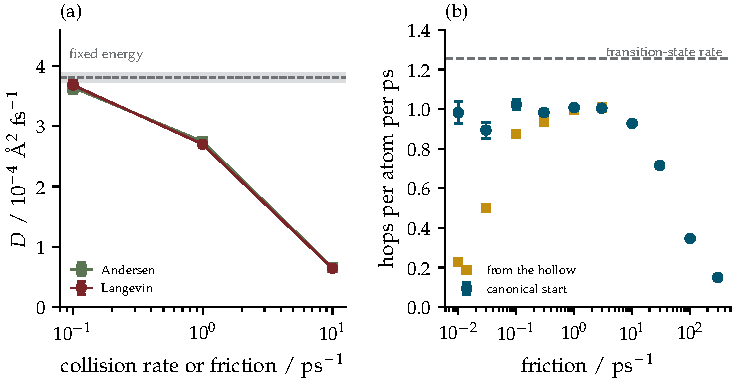
\includegraphics{ch13_thermostats/coupling}
\caption{(a) The diffusion coefficient of liquid argon, measured from the
centre of mass, against the collision rate of Andersen's thermostat and
the friction of Langevin's, each the mean of three runs with its
standard error, against three runs at fixed energy (line and band). (b)
Hops of lithium atoms between hollows of the model surface at
\SI{1000}{\kelvin}, per atom and picosecond, against the friction:
atoms started from the canonical distribution (circles, with the
standard error over the atoms) and atoms started at the bottom of a
hollow, counted over \SI{100}{\pico\second} (squares), against the rate of
transition-state theory (dashed).}
\label{fig:th-coupling}
\end{figure}

\begin{practice}
Langevin dynamics samples the canonical ensemble reliably, even for a
single atom, and is a good thermostat for averages over arrangements and
for equilibration. A friction of \SI{1}{\per\pico\second} already slows
the diffusion of liquid argon by more than a quarter; a diffusion coefficient or
a rate measured under Langevin dynamics belongs to the friction as much
as to the system, unless the friction is small against the system's own
rates of losing momentum.
\end{practice}

\begin{keyidea}
Friction and noise together give each velocity the exact step $v
\leftarrow cv + \sqrt{(1 - c^2)\kB T/m}\,g$, $c = \mathrm{e}^{-\gamma\dt}$,
whose noise is tied to the friction by $\sigma^2 = 2\gamma\kB T/m$. BAOAB
puts it between the half drifts of velocity Verlet and samples positions
accurately even at long steps. Friction slows diffusion and, for an atom
whose bath is the thermostat, sets its rate of hopping: about 0.8 of the
rate of transition-state theory at low friction, falling more and more
nearly in proportion to $1/\gamma$ at high.
\end{keyidea}

\notebook{13}{set the friction and watch diffusion and hopping change}

\begin{selfcheck}
What is $c$ for $\gamma = \SI{10}{\per\pico\second}$ and steps of
\SI{10}{\femto\second}, and what fraction of the velocity's variance is
replaced by fresh noise at each step?
\end{selfcheck}

%=============================================================================!
% 13.5  A FRICTION THAT LEARNS                                                !
%=============================================================================!
\section{A friction that learns}
\label{sec:th-nose}

Friction and noise disturb every atom at random. Nosé and Hoover found a
deterministic alternative: a single friction, shared by all the atoms,
that grows when the system is too hot and turns negative, pushing the
atoms faster, when it is too cold. This section gives their equations,
the quantity they conserve, why they sample the canonical ensemble when
the motion is ergodic, where they fail, and the chains that cure the
failure.

\subsection*{The equations}

Hoover's form of Nosé's thermostat adds one variable, the friction $\xi$,
with its own equation of motion\cite{Nose1984,Hoover1985}:
\begin{equation}
   \dot{\vb{r}}_i = \frac{\vb{p}_i}{m_i} , \qquad
   \dot{\vb{p}}_i = \vb{F}_i - \xi\,\vb{p}_i , \qquad
   \dot\xi = \frac{2K - N_{\mathrm f}\kB T_0}{Q} .
   \label{eq:th-nh}
\end{equation}
When $2K$ exceeds its canonical mean $N_{\mathrm f}\kB T_0$, $\xi$ grows and
the friction slows every atom; when $2K$ falls below, $\xi$ falls,
eventually below zero, and speeds them up. The thermostat's mass $Q$, an
energy times a time squared, sets how fast $\xi$ responds; with $Q =
N_{\mathrm f}\kB T_0\tau_{\mathrm T}^2$, $\tau_{\mathrm T}$ sets the time
over which it responds, a small departure of $K$ swinging with the period
$2\pi\tau_{\mathrm T}/\sqrt2$ (\cref{ex:th-nh-swing}); $Q$ is
\SI{8.9e4}{\electronvolt\femto\second\squared} for 256 argon atoms at
\SI{135}{\kelvin} with $\tau_{\mathrm T} = \SI{100}{\femto\second}$.

The motion keeps a quantity. With $H = K + U$, the force $-\xi\vb{p}_i$
changes $H$ at the rate $\sum_i\vb{p}_i\cdot(-\xi\vb{p}_i)/m_i = -2K\xi$,
while
\begin{equation*}
   \frac{\dd}{\dd t}\Bigl(\tfrac12Q\xi^2\Bigr) = Q\xi\dot\xi
   = \xi\bigl(2K - N_{\mathrm f}\kB T_0\bigr) ,
\end{equation*}
so
\begin{equation*}
   H + \tfrac12Q\xi^2 + N_{\mathrm f}\kB T_0\int_0^t\xi(t_1)\,\dd t_1
\end{equation*}
changes at the rate $-2K\xi + 2K\xi - N_{\mathrm f}\kB T_0\xi +
N_{\mathrm f}\kB T_0\xi = 0$. Its last two terms change at the rate
$2K\xi$, minus the rate at which the friction adds heat, so, with $\xi$
starting at zero, they are minus the heat, and this is the effective
energy of \cref{eq:th-effective}. One oscillator in reduced units,
followed for 1000 units of time, about 160 periods, with steps of 0.05,
starts with 0.2124 of it; the integrator's error makes it swing by up to
\num{9.4e-4} over the run, but it does not drift, and it ends
\num{4e-5} from where it began.

\subsection*{Why it is canonical}

\Cref{sec:ha-liouville} showed that the divergence of a flow is the rate
at which the volume of a small blob of states grows, divided by that
volume. In the space of positions, momenta and $\xi$, the rates
$\dot{\vb{r}}_i$ do not depend on $\vb{r}_i$, $\dot\xi$ does not depend on
$\xi$, and each of the $N_{\mathrm f}$ free momentum components has
$\partial\dot p/\partial p = -\xi$, the friction keeping a zero total
momentum at zero so that the motion stays among the free components; the
divergence is $-N_{\mathrm f}\xi$ (\cref{ex:th-divergence}).
A blob shrinks while $\xi > 0$, and since it keeps its copies, their
density along the flow rises at the rate $N_{\mathrm f}\xi$. The density
\begin{equation*}
   \rho \propto \mathrm{e}^{-\beta(H + \frac12Q\xi^2)} , \qquad
   \beta = \frac{1}{\kB T_0} .
\end{equation*}
changes along the flow at the rate
\begin{equation*}
   \frac{\dd\rho}{\dd t} = -\beta\rho\,\frac{\dd}{\dd t}\Bigl(H +
   \tfrac12Q\xi^2\Bigr) = -\beta\rho\,\bigl(-N_{\mathrm f}\kB T_0\xi\bigr)
   = N_{\mathrm f}\xi\rho ,
\end{equation*}
using the two rates above: the rate that the shrinking of the blobs
requires. The copies arriving at any state therefore have the density
this formula gives there, wherever they came from, so the cloud is the
same at every time, as for the Hamiltonian flow of
\cref{sec:ha-liouville}: the density is stationary. Integrating it over
$\xi$, a Gaussian, leaves
$\mathrm{e}^{-\beta H}$: the canonical distribution of the atoms. The
argument shows that the canonical ensemble is kept; that one trajectory
explores it, the ergodic hypothesis of \cref{sec:sm-ergodic}, is a
separate matter.

\subsection*{Nosé's Hamiltonian}

\Cref{eq:th-nh} came from a Hamiltonian. Nosé added a coordinate $s$
with momentum $p_s$, scaled the atoms' momenta by it, and took
\begin{equation*}
   H_{\mathrm N} = \sum_i\frac{\tilde{\vb{p}}_i^2}{2m_is^2} + U
   + \frac{p_s^2}{2Q} + N_{\mathrm f}\kB T_0\ln s ,
\end{equation*}
whose equations of motion, in a time $t'$ of their own, are Hamilton's.
Writing the real momenta as $\vb{p}_i = \tilde{\vb{p}}_i/s$, the real
time by $\dd t = \dd t'/s$, and $\xi = p_s/Q$, turns them into
\cref{eq:th-nh} (\cref{ex:th-nose}). The logarithm's slope,
$N_{\mathrm f}\kB T_0/s$, becomes the $-N_{\mathrm f}\kB T_0$ of $\dot\xi$
that sets the temperature; $s$ itself only records how the two times
differ.

\subsection*{Where it fails, and chains}

One oscillator, $H = \frac12p^2 + \frac12x^2$ in reduced units, under
\cref{eq:th-nh} with $\tau_{\mathrm T} = 1$, never fills its phase plane
(\cref{fig:th-nose}(a)): over 2000 units of time its positions have the
excess kurtosis of \cref{sec:sm-maxwell}, $\ens{x^4}/\ens{x^2}^2 - 3 =
-1.46$, against 0 for the canonical Gaussian. Started from 100 different positions at rest, each trajectory
keeps its own time average of $x^2$, from 0.78 to 1.59, where the
canonical value is 1 (\cref{fig:th-nose}(c)). The motion is not ergodic:
the single variable $\xi$ and the oscillator lock into a regular pattern.
A lithium atom on the surface with its own Nosé-Hoover thermostat fails
too: the density of its potential energy differs from the exact one, at
the worst point, by 0.23 of the exact density's peak, and it hops
\SI{0.667}{\per\pico\second}, against 1.09 under the chain of three
below, which samples it correctly.

Martyna, Klein and Tuckerman's cure gives $\xi$ a thermostat of its own,
and that one another, a chain\cite{Martyna1992}:
\begin{equation*}
   \dot\xi_1 = \frac{2K - N_{\mathrm f}\kB T_0}{Q_1} - \xi_2\xi_1 , \qquad
   \dot\xi_j = \frac{Q_{j-1}\xi_{j-1}^2 - \kB T_0}{Q_j} - \xi_{j+1}\xi_j ,
\end{equation*}
the last without the final term. The atoms feel only $\xi_1$, through
\cref{eq:th-nh}; each later $\xi_j$ is a friction on $\xi_{j-1}$, as
$\xi_1$ is on the atoms, driven by twice the energy
$\frac12Q_{j-1}\xi_{j-1}^2$ of $\xi_{j-1}$ against the $\kB T_0$ of one
freedom. The masses are $Q_1 = N_{\mathrm f}\kB T_0\tau_{\mathrm T}^2$ and,
for the others, $\kB T_0\tau_{\mathrm T}^2$. A chain of
four fills the oscillator's plane (\cref{fig:th-nose}(b)) and its
trajectories' averages of $x^2$ lie between 0.92 and 1.08; a chain of
three gives the lithium atom's density to within 0.016. \texttt{mdlab}
integrates the chain for half a step before and half after each step,
the Trotter factorisation of \cref{sec:in-splitting} with the thermostat
as a third part. Each half is made of three pieces, of $w_1$, $1 - 2w_1$
and $w_1$ times the half step, with $w_1 = 1/(2 - 2^{1/3}) = 1.3512$, so
that the middle piece runs backwards; these weights of
Yoshida\cite{Yoshida1990} cancel the error of third order. The scheme is
the one Martyna, Tuckerman, Tobias and Klein set out\cite{Martyna1996},
and ASE's. For the liquid tested here, the single thermostat and the chain
both give a spread of $K$ consistent with the canonical ensemble: the mean
of three runs lies between 0.0507 and 0.0534 at $\tau_{\mathrm T} = 0.1$
and \SI{1}{\pico\second}, against the canonical 0.0511, and the chain
costs about 1.1 times a step without a thermostat.

\begin{figure}[htb]
\centering
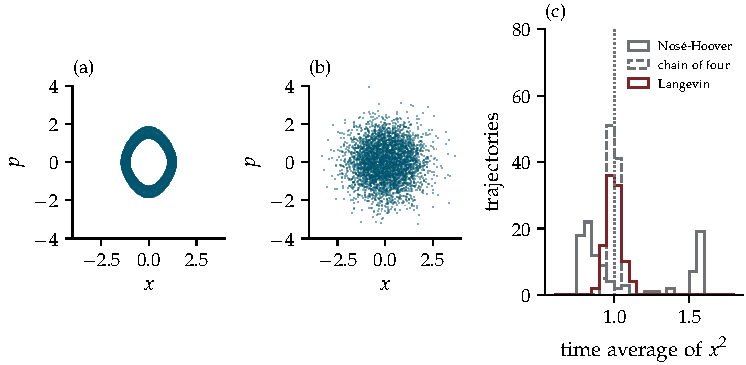
\includegraphics{ch13_thermostats/nose}
\caption{One oscillator ($m = k = \kB T_0 = 1$). (a) One trajectory under
Nosé-Hoover ($\tau_{\mathrm T} = 1$) over 2000 units of time, in the plane
of $x$ and $p$. (b) The same under a chain of four. (c) The time average
of $x^2$ along each of 100 trajectories started at rest from random
positions, under Nosé-Hoover, the chain and Langevin ($\gamma = 0.5$),
against the canonical value (dotted).}
\label{fig:th-nose}
\end{figure}

\begin{keyidea}
Nosé-Hoover friction $\xi$ obeys $\dot\xi = (2K - N_{\mathrm f}\kB T_0)/Q$
and keeps the effective energy. The density $\mathrm{e}^{-\beta(H +
Q\xi^2/2)}$ is carried unchanged by the flow, so the canonical ensemble is
stationary, but only an ergodic motion samples it: one oscillator, or one
atom in the examples here, is not sampled correctly by the single
thermostat. A chain samples these examples successfully. For the liquid
tested here, both give the canonical fluctuations and disturb the motion
little.
\end{keyidea}

\notebook{13}{follow one oscillator under Nosé-Hoover and under a chain}

\begin{selfcheck}
What is $Q_1$ for 1000 atoms whose centre of mass is held still, at \SI{300}{\kelvin}
with $\tau_{\mathrm T} = \SI{100}{\femto\second}$?
\end{selfcheck}

%=============================================================================!
% 13.6  RESCALING THAT SAMPLES                                                !
%=============================================================================!
\section{Rescaling that samples}
\label{sec:th-csvr}

Berendsen coupling disturbs the motion little but narrows the spread of
$K$; Langevin's friction gives the right spread but disturbs every atom.
Bussi, Donadio and Parrinello found a rescaling of all the velocities
together, like Berendsen's, that samples the canonical distribution
exactly\cite{Bussi2007}: canonical sampling through velocity rescaling,
CSVR. This section derives it from the exact step of
\cref{sec:th-langevin}, measures it, and reads TrajCast's implementation,
which holds its learned runs at a temperature.

\subsection*{The derivation}

In the $N_{\mathrm f}$ free components of \cref{sec:sm-equipartition},
mass-weighted so that $K = \frac12\lvert\vb{u}\rvert^2$, the velocities
form a vector $\vb{u}$. With the noise of \cref{eq:th-fdr}, the exact step
\cref{eq:th-ou} takes a velocity component $v$ to $cv + \sqrt{(1 -
c^2)\kB T_0/m}\,g$, and so $u = \sqrt m\,v$ to $cu + \sqrt{(1 - c^2)\kB
T_0}\,g$, whatever the mass. Applied to every component with the friction
$\gamma = 1/(2\tau_{\mathrm T})$, chosen so that the mean of $K$ relaxes
with the time constant $\tau_{\mathrm T}$, as shown below, and for which
$c^2 = \mathrm{e}^{-\dt/\tau_{\mathrm T}} = c_1$, it gives
\begin{equation*}
   \vb{u}' = \sqrt{c_1}\,\vb{u} + \sqrt{(1 - c_1)\kB T_0}\;\vb{g} ,
\end{equation*}
with $\vb{g}$ a vector of $N_{\mathrm f}$ independent normal numbers. Its
squared length is
\begin{equation*}
   \lvert\vb{u}'\rvert^2 = c_1\lvert\vb{u}\rvert^2 + (1 - c_1)\kB T_0\,
   \lvert\vb{g}\rvert^2 + 2\sqrt{c_1(1 - c_1)\kB T_0}\;\vb{u}\cdot\vb{g} .
\end{equation*}
The vector $\vb{g}$ can be resolved along $\vb{u}$ and at right angles to
it. Its density, the product of the factors $\mathrm{e}^{-g_k^2/2}$, is a
constant times $\mathrm{e}^{-\lvert\vb{g}\rvert^2/2}$, which depends only on
the length of $\vb{g}$; turning the axes, so that the first lies along
$\vb{u}$ and the others at right angles to it and to one another, leaves
that length, and so the density, unchanged, and the components of
$\vb{g}$ along the new axes are again independent normal numbers. So
$\vb{u}\cdot\vb{g} = \lvert\vb{u}\rvert R_1$, with $R_1$ the component of
$\vb{g}$ along $\vb{u}$, and $\lvert\vb{g}\rvert^2 = R_1^2 + R_\perp^2$,
with $R_\perp^2$ the sum of the squares of the other $N_{\mathrm f} - 1$ components,
independent of $R_1$. Dividing by $\lvert\vb{u}\rvert^2 = 2K$, which turns
the last term into $2R_1\sqrt{c_1(1 - c_1)\kB T_0/2K}$, and writing $c_2
= (1 - c_1)\kB T_0/2K = (1 - c_1)K_0/(N_{\mathrm f}K)$ (the names of Bussi
and colleagues, not the components $c_k$ of \cref{sec:sm-equipartition}),
\begin{equation}
   \frac{K'}{K} = \lambda^2 = c_1 + c_2\bigl(R_1^2 + R_\perp^2\bigr)
   + 2R_1\sqrt{c_1c_2} .
   \label{eq:th-csvr}
\end{equation}
CSVR keeps the change of $K$ that this step makes and throws away the
change of direction: it multiplies every velocity by $\lambda$. Since
$\lambda^2$ depends on the velocities only through $K$, the new $K$ has,
for a given $K$, the same distribution as after the whole
Ornstein-Uhlenbeck step. That step keeps the canonical distribution, every
component Gaussian with variance $\kB T_0$, and with it the gamma
distribution of $K$; so CSVR keeps that distribution too, for any $\dt$
and any $\tau_{\mathrm T}$. In the canonical density the direction of
$\vb{u}$ is spread evenly, independent of its length and of the
positions, and the scaling changes only the length; so, as with
Andersen's redraws, the whole canonical density is kept, and a run whose
motion is ergodic samples it to the accuracy of the step that moves the
atoms. Averaged over the noise
(\cref{ex:th-csvr-mean}), $\ens{K'} - K = (1 - c_1)(K_0 - K)$, the change
that $\dd K/\dd t = (K_0 - K)/\tau_{\mathrm T}$ makes over $\dt$; for a
short step $1 - c_1 \approx \dt/\tau_{\mathrm T}$, and this is the
relaxation of Berendsen coupling with the same time constant. The noise
supplies the canonical spread that Berendsen lacks. The sum $R_\perp^2$ of
$N_{\mathrm f} - 1$ squares need not be drawn square by square: by
\cref{eq:sm-gamma} with $\kB T = 1$ (\cref{ex:th-chi}), half of it has a
density proportional to $y^{(N_{\mathrm f} - 1)/2 - 1}\mathrm{e}^{-y}$,
the gamma distribution of shape $(N_{\mathrm f} - 1)/2$, from which NumPy
draws directly. \texttt{CSVR.before} is \cref{eq:th-csvr}:

\begin{code}
        k = kinetic(m, v, self.mv2_to_energy)
        target = 0.5 * self.n_free * self._kt(self.temperature)
        c1 = math.exp(-dt / self.tau)
        c2 = (1 - c1) * target / (k * self.n_free)
        r1 = rng.standard_normal(k.shape)
        rest = (2 * rng.standard_gamma(0.5 * (self.n_free - 1), k.shape)
                if self.n_free > 1 else np.zeros(k.shape))
        alpha2 = c1 + c2 * (rest + r1 * r1) + 2 * r1 * np.sqrt(c1 * c2)
        return v * np.sqrt(alpha2)[..., None, None]
\end{code}

\noindent Bussi and colleagues wrote the factor as $\alpha$, which is
$\lambda$ in this chapter; \texttt{alpha2} holds its square. At \SI{150}{\kelvin},
with a target of \SI{135}{\kelvin}, $\tau_{\mathrm T} =
\SI{100}{\femto\second}$ and steps of \SI{10}{\femto\second}, $c_1 =
0.90484$ and $c_2 = \num{1.120e-4}$, and with $R_1 = 0$ and $R_\perp^2$ at its
mean of 764, $\lambda^2 = 0.99037$, close to Berendsen's 0.9900.

\subsection*{Measured}

Over three runs of liquid argon the spread of $K$ is 0.0499 with
$\tau_{\mathrm T} = \SI{100}{\femto\second}$ and 0.0508 with
\SI{1}{\pico\second}, against the canonical 0.0511
(\cref{fig:th-berendsen}(a)); the diffusion coefficient is 1.07 and 1.05
times its value at fixed energy, a gap that \cref{sec:th-compare} weighs
against the scatter of the runs.
Acting once every three steps, over their whole length, with
$\tau_{\mathrm T} = \SI{300}{\femto\second}$, it still gives 0.0513.
For a single lithium atom, the density of the potential energy is within
0.012 of the exact one, and the atoms hop 1.08 times per picosecond. An
isolated molecule would show another side of the common factor: it keeps
its angular momentum under the forces, and CSVR's scaling multiplies it
at random, so TrajCast's authors set it to zero every hundred strides for
paracetamol\cite{Thiemann2026}.
CSVR scales every velocity by one factor, as Berendsen coupling does, but
its factor is not tilted towards growth\cite{Braun2018}, and a motion of
the centre of mass left in the velocities does not grow
(\cref{sec:th-trajectory}).

\subsection*{TrajCast's thermostat}

TrajCast predicts the state a stride $\Dt$ ahead, from
\SI{5}{\femto\second} for water to \SI{30}{\femto\second} for quartz in
the runs reported, and after each stride applies CSVR once, in the
file \texttt{\_thermostat.py} of its forecasting tools\cite{Thiemann2026},
whose lines 96-109 are \cref{eq:th-csvr}:

\begin{code}
        c2 = (
            (torch.tensor(1.0) - self.c1) * e_kin_target
            / e_kin_current / self.n_dofs
        ).to(self.device)
        r1 = torch.randn(1, device=self.device)
        r2 = self._draw_sum_noises_from_gamma_dist(n_dofs_1=self.n_dofs - 1)
        alpha_2 = (
            self.c1
            + c2 * (r1 * r1 + r2)
            + torch.tensor(2.0) * r1 * (self.c1 * c2).sqrt()
        )
\end{code}

\noindent with comments removed and one line wrapped. \texttt{c1} is $\mathrm{e}^{-\Dt/\tau_{
\mathrm T}}$, computed once with the stride as the step (lines 32-37);
\texttt{r2} is $R_\perp^2$, drawn as twice a gamma number of shape $(N_{\mathrm f} -
1)/2$, or, when $N_{\mathrm f} - 1$ is odd, as twice one of shape
$(N_{\mathrm f} - 2)/2$ plus one more square (lines 113-123), which is the
same distribution; and \texttt{n\_dofs} is $3N$ less three for each kind
of momentum, linear or angular, that the run removes or holds fixed, or
less a number the run's settings give (\texttt{forecast.py}, lines
344-378).
With no time constant given, $\tau_{\mathrm T}$ is a hundred strides, so
$c_1 = \mathrm{e}^{-0.01} = 0.9900$ and the temperature is held loosely;
the runs reported used ten strides for water and paracetamol, 50 and
\SI{70}{\femto\second}, $c_1 = 0.9048$, and two and a half for quartz,
\SI{75}{\femto\second}, $c_1 = 0.6703$. Since \cref{eq:th-csvr} keeps the
distribution of $K$ for any step, the thermostat itself works at any
stride, as the run acting once every three steps confirmed. The stride
changes what the thermostat corrects: a learned step may not keep the
energy, and CSVR would then remove the error as heat, so in a learned run
the heat may measure the model's error as well as the bath's work, a
theme of the planned Part~VI. TrajCast's authors found that the longer strides needed
much shorter $\tau_{\mathrm T}$ than usual to hold the temperature and its
spread, and put it down to each stride standing for several steps taken
before one rescaling\cite{Thiemann2026}.

\begin{keyidea}
CSVR applies the exact Ornstein-Uhlenbeck step to all $N_{\mathrm f}$
mass-weighted velocity components at once, keeps only its change of
length, and scales every velocity by the factor $\lambda$ of
\cref{eq:th-csvr}. Its step then keeps the canonical gamma distribution of
$K$ for any step and coupling, the mean relaxes as under Berendsen
coupling, and the motion is disturbed as little as by Berendsen
coupling. TrajCast applies it once per
learned stride, with $c_1 = \mathrm{e}^{-\Dt/\tau_{\mathrm T}}$.
\end{keyidea}

\notebook{13}{set the coupling and the stride, and compare CSVR with Berendsen}

\begin{selfcheck}
For TrajCast's stride of \SI{30}{\femto\second} for quartz, what
$\tau_{\mathrm T}$ gives $c_1 = 0.5$?
\end{selfcheck}

%=============================================================================!
% 13.7  WHICH THERMOSTAT, AND WHEN                                            !
%=============================================================================!
\section{Which thermostat, and when}
\label{sec:th-compare}

The sections so far measured each thermostat on its own. This section
sets the measurements side by side and draws from them which thermostat
to use for the three jobs a thermostat does: bringing a system to a
temperature, sampling averages at it, and leaving its dynamics fit to
measure.

\subsection*{Side by side}

\Cref{tab:th-compare} collects, for every thermostat and coupling, the
spread of $K$ in liquid argon as a fraction of the canonical spread, the
diffusion coefficient as a fraction of its value at fixed energy, and,
for one lithium atom with its own thermostat, how far the density of its
potential energy misses the exact one and how often it hops. The
diffusion coefficients carry the standard error of three runs, the
standard deviation of their three estimates divided by $\sqrt3$, since the variances of
the three add and their mean divides the sum by three; with so few runs it
is itself rough, and Chapter~15 gives the tools to say when two such
numbers differ. Three groups stand out.
\begin{itemize}
\item Rescaling fixes the kinetic temperature at each rescaling, and Berendsen
   coupling keeps its mean close to the target. Both narrow the spread, 0.11 to 0.59 of the canonical, and a single atom
   under Berendsen coupling stops hopping.
\item Andersen and Langevin sample the canonical ensemble once the
   coupling is \SI{1}{\per\pico\second} or more, for the liquid and for
   one atom alike, and cost no more than a step without a thermostat. At
   that coupling they cut the diffusion coefficient to 0.71 to 0.72 of its
   value, and at \SI{10}{\per\pico\second} to 0.17.
\item Nosé-Hoover chains and CSVR give the canonical spread at both
   couplings and sample one atom correctly. Like Berendsen coupling and a
   single Nosé-Hoover thermostat, they leave the diffusion coefficient
   1.01 to 1.07 of its value at fixed energy, in runs 0.4 to
   \SI{1.8}{\kelvin} warmer than those at fixed energy. The variances of
   independent quantities add, so the standard error of a difference is
   the square root of the sum of the two squared standard errors; the
   chains and CSVR lie at most 2.5 of these from fixed energy, and
   Berendsen coupling at \SI{1}{\pico\second} 2.9. Whether so small a
   difference is real is a question for Chapter~15. A single Nosé-Hoover thermostat matches the chains for
   the liquid but not for one atom. These findings agree with Basconi and
   Shirts, who compared thermostats on the transport properties of
   liquids\cite{Basconi2013}.
\end{itemize}

\begin{table}[htb]
\centering
\caption{The thermostats measured: for liquid argon at \SI{135}{\kelvin},
the relative spread of $K$ divided by the canonical
$\sqrt{2/N_{\mathrm f}}$, and
the diffusion coefficient divided by its value at fixed energy,
$(3.81\pm0.08)\times10^{-4}$\,\AA$^2$/fs (three runs of
\SI{100}{\pico\second}; rescaling, one); for one lithium atom on the
surface at \SI{1000}{\kelvin}, the largest gap between the density of its
potential energy and the exact one, divided by the exact density's peak,
and its hops per picosecond (1000 atoms over \SI{100}{\pico\second}).
For Andersen and Langevin, which move the centre of mass, $N_{\mathrm f} =
3N = 768$. Under Berendsen coupling the density is a narrow spike, so its
gap is many times the peak.}
\label{tab:th-compare}
\small
\begin{tabular}{@{}lllll@{}}
\toprule
& \multicolumn{2}{l}{liquid argon} & \multicolumn{2}{l}{one lithium atom}\\
thermostat & spread & $D$ & gap & hops/ps\\
\midrule
fixed energy & 0.61 & 1 & & \\
rescaling & 0.11 & 1.01 & & \\
Berendsen, \SI{0.1}{\pico\second} & 0.45 & $1.04\pm0.01$ & 15.5 & 0.001\\
Berendsen, \SI{1}{\pico\second} & 0.59 & $1.07\pm0.01$ & & \\
Andersen, \SI{0.1}{\per\pico\second} & 0.85 & $0.96\pm0.03$ & & \\
Andersen, \SI{1}{\per\pico\second} & 0.98 & $0.72\pm0.01$ & 0.011 & 0.974\\
Andersen, \SI{10}{\per\pico\second} & 1.00 & $0.173\pm0.004$ & & \\
Langevin, \SI{0.1}{\per\pico\second} & 0.93 & $0.97\pm0.02$ & 0.024 & 1.024\\
Langevin, \SI{1}{\per\pico\second} & 1.01 & $0.71\pm0.01$ & 0.005 & 1.008\\
Langevin, \SI{10}{\per\pico\second} & 1.01 & $0.169\pm0.001$ & 0.008 & 0.928\\
Nosé-Hoover, \SI{0.1}{\pico\second} & 0.99 & $1.02\pm0.01$ & 0.231 & 0.667\\
Nosé-Hoover, \SI{1}{\pico\second} & 1.04 & $1.05\pm0.01$ & & \\
chain of 3, \SI{0.1}{\pico\second} & 1.01 & $1.04\pm0.03$ & 0.016 & 1.087\\
chain of 3, \SI{1}{\pico\second} & 1.01 & $1.01\pm0.02$ & & \\
CSVR, \SI{0.1}{\pico\second} & 0.98 & $1.07\pm0.02$ & 0.012 & 1.081\\
CSVR, \SI{1}{\pico\second} & 0.99 & $1.05\pm0.01$ & & \\
\bottomrule
\end{tabular}
\end{table}

\subsection*{What to use}

\Cref{tab:th-choose} turns the measurements into a choice for each job.

\emph{Bringing a system to a temperature.} Any thermostat does it; what
matters is how fast it gets there and that it settles at the target. From
\SI{200}{\kelvin}, Berendsen and CSVR with $\tau_{\mathrm T} =
\SI{1}{\pico\second}$ and Langevin with $\gamma = \SI{1}{\per\pico\second}$
all reach the target within a few picoseconds (\cref{fig:th-berendsen}(b)).
Under Berendsen and CSVR the excess decays with the time constant
$\tau_{\mathrm T}C_V/C_K = \SI{1.59}{\pico\second}$, fitted at 1.67 and
\SI{1.63}{\pico\second}; under Langevin with $C_V/(2\gamma C_K) =
\SI{0.80}{\pico\second}$, fitted at \SI{0.68}{\pico\second}
(\cref{ex:th-langevin-tau}). A short coupling time, 0.1 to
\SI{1}{\pico\second}, is right here, and the run's early part is
discarded, for which Chapter~15 gives a measured criterion.

\emph{Averages at a temperature.} The average and the fluctuations must
both be canonical, so rescaling and Berendsen coupling are out. CSVR,
Nosé-Hoover chains, Langevin and Andersen all qualify. A single
Nosé-Hoover thermostat failed for one oscillator and for one atom on the
surface, and is expected to fail likewise for other small or nearly
harmonic systems, a single molecule or a nearly harmonic
crystal\cite{Martyna1992}. The heat capacity from the energy's
fluctuations, \cref{eq:sm-fluctuation}, shows what is at stake: it comes
out at 2.28 to $2.40N\kB$ under CSVR, the chain and Langevin, against the
$2.376N\kB$ of Chapter~12 from $\dd E/\dd T$, and at $0.41N\kB$ under
Berendsen coupling with $\tau_{\mathrm T} = \SI{0.1}{\pico\second}$.

\emph{Dynamics.} The thermostat must disturb the motion as little as
possible; of the motion, this chapter measured the diffusion of the
liquid. A run at fixed energy started from an equilibrated state disturbs
nothing, but its temperature is the one its energy gives, which in our
runs fell \SI{0.66}{\kelvin} short. CSVR or a Nosé-Hoover chain changes
the diffusion of the liquid by at most 7\%, and a coupling time of a
picosecond or more keeps the thermostat's hand light. Berendsen coupling
changes it no more, but it narrows the fluctuations, feeds the flying ice
cube and pins a single atom. Langevin and Andersen thermostats at
\SI{1}{\per\pico\second} remove more than a quarter of it.

\emph{An atom whose only bath is the thermostat.} When the real bath is
left out, as for an atom on a frozen surface, the thermostat's coupling
becomes part of the physics: the lithium atom's hop rate fell from 1.0 to
\SI{0.35}{\per\pico\second} as the friction rose from 3 to
\SI{100}{\per\pico\second}. Such a rate means something only
if the friction stands for a real bath, and the safer course is to
simulate the bath's atoms.

\begin{table}[htb]
\centering
\caption{Which thermostat to use, from the measurements of this chapter.}
\label{tab:th-choose}
\small
\begin{tabular}{@{}>{\raggedright\arraybackslash}p{0.25\linewidth}
   >{\raggedright\arraybackslash}p{0.38\linewidth}
   >{\raggedright\arraybackslash}p{0.3\linewidth}@{}}
\toprule
job & use & avoid\\
\midrule
bringing to a temperature & Berendsen, CSVR or Langevin,
   $\tau_{\mathrm T}$ of 0.1 to \SI{1}{\pico\second} or $\gamma$ of 1 to
   \SI{10}{\per\pico\second} (measured at \SI{1}{\pico\second} and
   \SI{1}{\per\pico\second}), the early part discarded & one Berendsen
   thermostat on a single atom, which pins its energy\\
averages and fluctuations & CSVR, Nosé-Hoover chains, Langevin, Andersen
   & rescaling, Berendsen; one Nosé-Hoover thermostat on small or nearly
   harmonic systems\\
dynamics (here, diffusion) & fixed energy after equilibrating; CSVR or a
   chain with $\tau_{\mathrm T} \ge \SI{1}{\pico\second}$ & Langevin and
   Andersen at $\ge$ \SI{1}{\per\pico\second}; Berendsen, for its
   fluctuations and flying ice cube\\
learned runs (TrajCast) & CSVR once per stride; its update preserves the canonical
   distribution of $K$ & Berendsen\\
\bottomrule
\end{tabular}
\end{table}

\begin{keyidea}
Rescaling and Berendsen coupling are for reaching a temperature. CSVR,
Nosé-Hoover chains, Langevin and Andersen sample the canonical ensemble; of
these,
CSVR and chains change the diffusion of the liquid by at most 7\%, while
friction or collisions at \SI{1}{\per\pico\second} slow it by more than
a quarter. A single Nosé-Hoover thermostat fails for small systems, and
for an atom whose bath is the thermostat, the atom's rates belong to the
coupling.
\end{keyidea}

\begin{selfcheck}
A run is to measure the diffusion of lithium in a liquid electrolyte at
\SI{300}{\kelvin}. Which thermostat, with what coupling, does this chapter
recommend for the production run, and why not Langevin with $\gamma =
\SI{5}{\per\pico\second}$?
\end{selfcheck}

%=============================================================================!
% 13.8  WHAT THE TRAJECTORY LOOKS LIKE                                        !
%=============================================================================!
\section{What the trajectory looks like}
\label{sec:th-trajectory}

A thermostat changes what a healthy run looks like: the energy is no
longer constant, and the temperature should fluctuate by a definite
amount. This section shows a healthy thermostatted run of liquid argon
and six faults that thermostats leave, each with the check that catches
it.

\subsection*{A healthy run}

\Cref{fig:th-healthy} follows the liquid under CSVR with $\tau_{\mathrm T}
= \SI{100}{\femto\second}$ for \SI{100}{\pico\second}. From
\SI{5}{\pico\second} on, its kinetic temperature averages
\SI{135.57}{\kelvin}, with a relative spread of 0.0486 against the
canonical 0.0511, and lies within one canonical spread of the target
for 0.719 of the time, close to the 0.683 of a Gaussian
(\cref{sec:sm-probability}). The total energy is no longer kept: it
wanders over \SI{9.17}{\milli\electronvolt} per atom as the thermostat
exchanges heat. The effective energy of \cref{eq:th-effective} stays
within \SI{0.018}{\milli\electronvolt} per atom, five hundred times less,
and falls by \SI{1.6e-5}{\electronvolt\per\pico\second} for the whole
box: it plays the
part the total energy played in \cref{sec:cs-trajectory}. The total
momentum stays below \SI{4e-14}{amu\,\angstrom\per\femto\second}, since
CSVR scales a zero momentum to zero, and the histogram of $K$ follows the
gamma density.

\begin{figure}[htb]
\centering
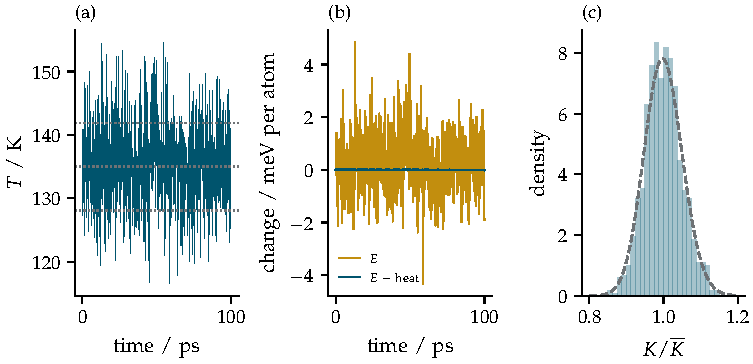
\includegraphics{ch13_thermostats/healthy}
\caption{A healthy thermostatted run: liquid argon under CSVR with
$\tau_{\mathrm T} = \SI{100}{\femto\second}$ for \SI{100}{\pico\second}.
(a) The kinetic temperature every \SI{100}{\femto\second}, with the
target and one canonical spread either side (dotted). (b) The total
energy and the effective energy per atom, from their starting values. (c)
The kinetic energy over the run, divided by its mean, against the
canonical gamma density (dashed).}
\label{fig:th-healthy}
\end{figure}

\subsection*{Six faults}

\Cref{fig:th-faults} shows six faults and \cref{tab:th-faults} the check
that catches each.

\begin{figure}[p]
\centering
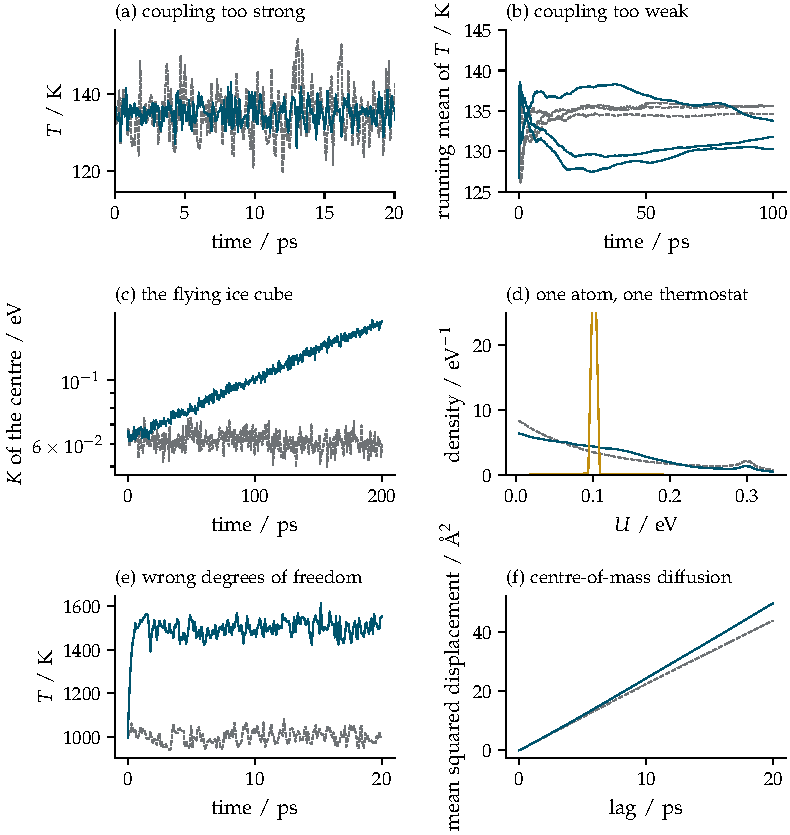
\includegraphics{ch13_thermostats/faults}
\caption{Thermostat faults (teal) against healthy runs (grey dashed). (a)
Liquid argon under Berendsen coupling with $\tau_{\mathrm T} =
\SI{100}{\femto\second}$, against CSVR. (b) The running mean of the
temperature in three runs under Andersen's thermostat at
\SI{0.1}{\per\pico\second}, against three under CSVR. (c) The kinetic
energy of the motion of the centre of mass, started moving, under
Berendsen coupling, against CSVR, on a logarithmic axis. (d) The density
of the potential energy of lithium atoms on the surface, each under its
own Nosé-Hoover thermostat (teal) or Berendsen thermostat (ochre, cut
off), against the exact canonical density. (e) Lithium atoms under CSVR
told $N_{\mathrm f} = 3$: their kinetic temperature over the two freedoms
they have, against CSVR told 2. (f) The mean squared displacement in
liquid argon under Langevin dynamics with $\gamma = \SI{0.1}{\per\pico
\second}$, measured in the cell, against measured from the centre of
mass.}
\label{fig:th-faults}
\end{figure}

\begin{table}[htb]
\centering
\caption{The faults of \cref{fig:th-faults}, the check that catches each,
and its value in the healthy and the broken run; (a) uses the first of
the three runs, so its spreads differ slightly from the three-run means of
\cref{tab:th-compare}.}
\label{tab:th-faults}
\small
\begin{tabular}{@{}llll@{}}
\toprule
fault & check & healthy & broken\\
\midrule
(a) coupling too strong & spread of $T$ / canonical & 0.95 & 0.44\\
(b) coupling too weak & mean $T$ of three runs, K &
   $135.38\pm0.31$ & $131.83\pm1.02$\\
(c) flying ice cube & growth of $\ln K_{\mathrm{com}}$, /ps & $-0.0002$ &
   0.0047\\
(d) one atom, one variable & gap from the exact density & 0.016 & 0.231\\
(e) wrong $N_{\mathrm f}$ & $T$ over the true freedoms, K & 1005 & 1506\\
(f) centre as diffusion & $D$, $10^{-4}$\,\AA$^2$/fs & 3.69 & 4.62\\
\bottomrule
\end{tabular}
\end{table}

\emph{(a) Coupling too strong.} Berendsen coupling with $\tau_{\mathrm T} =
\SI{100}{\femto\second}$ holds the temperature in a band 0.44 as wide as
the canonical one; CSVR with the same time constant gives 0.95. The
average looks perfect, \SI{135.00}{\kelvin}, and only the spread shows
the fault: the check is the relative spread of $T$ against
$\sqrt{2/N_{\mathrm f}}$.

\emph{(b) Coupling too weak.} Andersen's thermostat at
\SI{0.1}{\per\pico\second} lets the temperature wander for tens of
picoseconds: three runs average 133.66, 130.13 and
\SI{131.69}{\kelvin}, counting all $3N$ freedoms, against 135.58, 134.77 and \SI{135.79}{\kelvin}
under CSVR. Nothing in one run looks wrong; the check is the spread of
the run means between independent starts, or the running mean's failure
to settle near the target.

\emph{(c) The flying ice cube.} A velocity of the centre of mass of
\SI{0.0002}{\angstrom\per\femto\second} in each component, left in the
velocities, gives the centre of mass the kinetic energy $K_{\mathrm{com}}$,
whose logarithm grows under Berendsen coupling at
\SI{0.0047}{\per\pico\second}, against the \SI{0.0050}{\per\pico\second}
predicted in \cref{sec:th-berendsen}: $K_{\mathrm{com}}$ rises from
\SI{0.064}{\electronvolt} to \SI{0.161}{\electronvolt} in
\SI{200}{\pico\second}; under CSVR it does not grow. The check is the
kinetic energy of the centre of mass, and of the slowest motions, over a
long run.

\emph{(d) One atom, one variable.} A lithium atom with its own
Nosé-Hoover thermostat misses the exact density of its potential energy
by 0.231 of its peak; with a chain of three, by 0.016; under Berendsen
coupling it is pinned near one energy. The check is a distribution
compared with an exact or independently sampled one, here the density of
$U$; for a large system, the temperatures of its parts
(\cref{sec:sm-trajectory}).

\emph{(e) The wrong number of freedoms in the target.} A thermostat told
three freedoms per lithium atom, which has two, drives each atom's
kinetic energy to $\frac32\kB T_0$, so its true temperature reads
\SI{1506}{\kelvin} for a target of \SI{1000}{\kelvin}. The same fault in
a large system is small but systematic: a thermostat that takes $3N$
freedoms for a run whose centre of mass is held still, as ASE's Berendsen, CSVR and
Nosé-Hoover chain do for argon, raises the temperature of 256 atoms by the
factor $768/765$, \SI{0.5}{\kelvin} at \SI{135}{\kelvin}, about the
scatter between independent runs. For rigid water a thermostat that also
ignores the held distances, as ASE's Nosé-Hoover chain does, raises it by
$576/381 = 1.51$ (\cref{sec:sm-trajectory}); ASE's CSVR and Berendsen
subtract the held distances and miss only the three freedoms of the centre of mass, $384/381$.
The check is the kinetic temperature computed with the freedoms counted
for the run.

\emph{(f) The centre of mass counted as diffusion.} Langevin and Andersen
thermostats do not keep the total momentum, so the centre of mass
wanders; under Langevin dynamics it diffuses, over times long against
$1/\gamma$, with the coefficient $\kB T/(M\gamma)$, which for the whole
box at $\gamma = \SI{0.1}{\per\pico\second}$ is
\SI{1.10e-4}{\angstrom\squared\per\femto\second}
(\cref{ex:th-com}). Displacements measured in the cell include it: the
diffusion coefficient reads $4.62\times10^{-4}$ instead of
$3.69\times10^{-4}$\,\AA$^2$/fs, 1.25 times too large. The check is to measure displacements from the centre of mass.

\begin{practice}
A thermostatted run is read through its kinetic temperature, whose
spread should be $\sqrt{2/N_{\mathrm f}}$ of the target when the freedoms
are counted for the run; through its effective energy, which should
neither wander nor drift; through the kinetic energy of its centre of
mass and of its slowest motions, which should not grow; and, for a
property that depends on the motion, through the same property with the
thermostat weakened, which should not change. Runs from several
independent starts show whether a weakly coupled run has reached its
temperature, a question Chapter~15 answers with error bars.
\end{practice}

\begin{keyidea}
In a healthy thermostatted run the total energy wanders, the effective
energy holds still, the temperature fluctuates by the canonical
$\sqrt{2/N_{\mathrm f}}$, and the centre of mass stays still or is
measured from. Coupling too strong narrows the spread; too weak leaves the
mean unsettled; rescaling and Berendsen coupling fly the ice cube; a single Nosé-Hoover
variable fails on small systems; a miscounted $N_{\mathrm f}$ shifts the
temperature; and a wandering centre of mass inflates diffusion.
\end{keyidea}

\notebook{13}{break the thermostatted liquid in each of the six ways and read the checks}

\begin{selfcheck}
A Langevin run of 500 argon atoms with $\gamma = \SI{1}{\per\pico\second}$
at \SI{135}{\kelvin}: at what rate does its centre of mass diffuse?
\end{selfcheck}

%=============================================================================!
% 13.S  WHAT WE NOW HAVE                                                      !
%=============================================================================!
\unnumbered{What we now have}

A thermostat must give the canonical distributions, the gamma
distribution of $K$ with spread $\sqrt{2/N_{\mathrm f}}$ and the density
$\mathrm{e}^{-\beta U}$ of positions, and should disturb the motion as
little as possible; the effective energy, $K + U$ less the heat it adds,
is kept by the exact dynamics of every thermostat and checks the
integration.

Every method of the chapter fits one loop, velocity Verlet
written as B A A B, with the thermostat acting before, between the half
drifts or after; four of the five that ASE also implements agree with its
versions to \SI{1e-7}{\angstrom}, and Andersen's in the temperature it
holds.

Rescaling and Berendsen coupling hold the mean temperature but narrow the
spread of $K$ to 0.11 to 0.59 of the canonical, and feed motions that the
forces do not touch at the rate $\ens{(\delta T/T_0)^2}/\tau_{\mathrm T}$,
the flying
ice cube, measured at \SI{0.0047}{\per\pico\second} against
\SI{0.0050}{\per\pico\second} predicted.

Andersen's collisions, and
Langevin's friction and noise, tied by $\sigma^2 = 2\gamma\kB T/m$ and
integrated exactly by the O step of BAOAB, sample the canonical ensemble
even for one atom, and slow the diffusion of liquid argon by more than a
quarter at \SI{1}{\per\pico\second}; for an atom whose only bath is the
thermostat, Langevin's friction sets the hop rate, near 0.8 of the
transition-state rate at low friction and falling more and more nearly
in proportion to $1/\gamma$ at high.

Nosé-Hoover friction keeps an extended energy and carries the
canonical density unchanged, but samples it only for an ergodic motion,
so one oscillator or one atom fails where a chain succeeds.

CSVR applies
the exact Ornstein-Uhlenbeck step to the length of the whole
mass-weighted velocity, so its thermostat update preserves the canonical distribution of $K$
for any step and coupling. TrajCast can therefore apply that update once
per learned stride, while the intervening propagation remains a separate
source of sampling error.

For bringing
a system to a temperature any thermostat serves; for averages, CSVR,
chains, Langevin or Andersen; for dynamics, a run at fixed energy, or CSVR or a
chain coupled weakly.

Chapter~14 does for pressure what this chapter did for temperature:
derives the pressure from the virial, and builds the barostats that hold
it.

%=============================================================================!
% 13.A  ANSWERS TO THE CHECKS                                                 !
%=============================================================================!
\unnumbered{Answers to the checks}
\label{sec:th-answers}

\answerto{sec:th-tests}The heat is \SI{-0.5}{\electronvolt}, so
$E_{\mathrm{eff}}$ changes by $-0.48 - (-0.5) = \SI{+0.02}{\electronvolt}$:
the integration has added \SI{0.02}{\electronvolt}.

\answerto{sec:th-berendsen}$\lambda^2 = 1 + 0.002\,(300/310 - 1) =
0.9999355$, so $\lambda = 0.9999677$.

\answerto{sec:th-andersen}$1 - \mathrm{e}^{-0.002} = 0.001998$, so about 2
atoms of 1000 at each step.

\answerto{sec:th-langevin}$c = \mathrm{e}^{-0.1} = 0.90484$; the old
velocity keeps the fraction $c^2$ of its variance, so $1 - c^2 = 0.181$ is
replaced by noise.

\answerto{sec:th-nose}$N_{\mathrm f} = 2997$ and $\kB T_0 =
\SI{0.025852}{\electronvolt}$, so $Q_1 = 2997\times0.025852\times100^2 =
\SI{7.75e5}{\electronvolt\femto\second\squared}$.

\answerto{sec:th-csvr}$\mathrm{e}^{-30/\tau_{\mathrm T}} = 0.5$ gives
$\tau_{\mathrm T} = 30/\ln2 = \SI{43.3}{\femto\second}$.

\answerto{sec:th-compare}CSVR, or a Nosé-Hoover chain, with $\tau_{\mathrm
T}$ of a picosecond or more, or a run at fixed energy after equilibrating:
in liquid argon the first two changed diffusion by at most 7\%, the last
not at all. Langevin at \SI{5}{\per\pico\second} would slow it by well
over a quarter, leaving between the 0.71 and 0.17 of it measured at 1 and
\SI{10}{\per\pico\second}.

\answerto{sec:th-trajectory}$\kB T/(M\gamma)$, with $\kB T =
\SI{0.011633}{\electronvolt}$ at \SI{135}{\kelvin}, $M = 500\times39.948 =
\SI{19974}{\amu}$, $\gamma = \SI{0.001}{\per\femto\second}$ and the
factor 103.6427 of \cref{eq:en-mv2}:
\begin{equation*}
   \frac{0.011633}{19\,974\times103.6427\times0.001}
   = \SI{5.6e-6}{\angstrom\squared\per\femto\second} .
\end{equation*}

%=============================================================================!
% 13.E  EXERCISES                                                             !
%=============================================================================!
\unnumbered{Exercises}
\label{sec:th-exercises}

The exercises run from questions of understanding, through calculations,
to short derivations marked `show that'. Full solutions are in
\hyperref[sec:th-solutions]{`Solutions to the exercises'} at the end of
the book, and Notebook~13 checks every numerical answer.

\begin{exercise}[collisions in a step]
\label{ex:th-collisions}
Collisions come at the rate $\nu$, independently in every short interval.
Show, by cutting a step $\dt$ into $n$ intervals each with the collision
probability $\nu\dt/n$, that the probability of no collision in the step
is $\mathrm{e}^{-\nu\dt}$. What is the probability of at least one for
$\nu = \SI{1}{\per\pico\second}$ and $\dt = \SI{2}{\femto\second}$?
\end{exercise}

\begin{exercise}[one Berendsen step]
\label{ex:th-lambda}
Find $\lambda$ for a step of \SI{1}{\femto\second}, $\tau_{\mathrm T} =
\SI{0.5}{\pico\second}$, a kinetic temperature of \SI{290}{\kelvin} and a
target of \SI{300}{\kelvin}.
\end{exercise}

\begin{exercise}[the mean under Berendsen]
\label{ex:th-mean}
Show that a run under Berendsen coupling that has settled, so that the
heat it receives averages to zero, has $\ens{T} = T_0$ exactly.
\end{exercise}

\begin{exercise}[how fast Langevin cools]
\label{ex:th-langevin-tau}
Show from \cref{eq:th-ou} that under Langevin dynamics the heat flows in
at the rate $2\gamma(K_0 - K)$ when the forces are ignored for the moment,
and hence that a liquid's temperature relaxes with the time constant
$C_V/(2\gamma C_K)$. Give it for liquid argon at $\gamma =
\SI{1}{\per\pico\second}$.
\end{exercise}

\begin{exercise}[how far the ice cube flies]
\label{ex:th-ice}
Under Berendsen coupling with $\tau_{\mathrm T} = \SI{0.1}{\pico\second}$
and $\ens{(\delta T/T_0)^2} = \num{5e-4}$, by what factor does the kinetic energy of
the centre of mass grow in \SI{1}{\nano\second}?
\end{exercise}

\begin{exercise}[sums of Gaussians]
\label{ex:th-gauss-sum}
Show that if $x$ and $y$ are independent and Gaussian with mean zero and
variances $a$ and $b$, then $x + y$ is Gaussian with variance $a + b$,
by finding the density of $s = x + y$, $\int\mathcal{P}(x)\mathcal{P}(s -
x)\,\dd x$, and completing the square in $x$.
\end{exercise}

\begin{exercise}[the variance settles]
\label{ex:th-ou-variance}
Show from \cref{eq:th-ou} that the variance of $v$ after one step is
$c^2$ times the variance before plus $(\sigma^2/2\gamma)(1 - c^2)$, and
that $\sigma^2/2\gamma$ is the only variance that a step leaves unchanged.
\end{exercise}

\begin{exercise}[the noise in a step]
\label{ex:th-noise}
For argon at \SI{135}{\kelvin}, $\gamma = \SI{1}{\per\pico\second}$ and
steps of \SI{10}{\femto\second}, find the standard deviation of the
random part of one O step, $\sqrt{(1 - c^2)\kB T/m}$, in
\si{\angstrom\per\femto\second}.
\end{exercise}

\begin{exercise}[no friction, no noise]
\label{ex:th-baoab-vv}
Show that BAOAB with $\gamma = 0$ is velocity Verlet.
\end{exercise}

\begin{exercise}[the outward flux]
\label{ex:th-flux}
Show that
\begin{equation*}
   \int_0^\infty v\,\mathrm{e}^{-mv^2/2\kB T}\dd v\Big/\sqrt{2\pi\kB T/m}
   = \sqrt{\kB T/2\pi m} ,
\end{equation*}
and find it for lithium at \SI{1000}{\kelvin}.
\end{exercise}

\begin{exercise}[transition-state theory in one dimension]
\label{ex:th-tst-1d}
For an atom in one dimension in a well that is harmonic near its bottom,
$U \approx \frac12m\omega^2x^2$, with a barrier $U_{\mathrm b}$ on one
side, show that the one-dimensional form of \cref{eq:th-tst} gives
$k_{\mathrm{TST}} \approx (\omega/2\pi)\,\mathrm{e}^{-U_{\mathrm b}/\kB
T}$ when $U_{\mathrm b} \gg \kB T$. Evaluate it for the lithium atom's
period of \SI{170.3}{\femto\second} and $U_{\mathrm b} =
\SI{0.3}{\electronvolt}$ at \SI{300}{\kelvin}, in hops per second.
\end{exercise}

\begin{exercise}[the friction's own swing]
\label{ex:th-nh-swing}
Ignoring the forces, so that only the friction changes $K$, show that
small departures $\delta K$ of $K$ from $K_0 = \frac12N_{\mathrm f}\kB T_0$
under \cref{eq:th-nh}, with $Q = N_{\mathrm f}\kB T_0\tau_{\mathrm T}^2$,
obey
\begin{equation*}
   \frac{\dd^2\,\delta K}{\dd t^2} = -\frac{2}{\tau_{\mathrm T}^2}\,\delta K .
\end{equation*}
What is the period for $\tau_{\mathrm T} = \SI{100}{\femto\second}$?
\end{exercise}

\begin{exercise}[from Nosé to Hoover]
\label{ex:th-nose}
Write Hamilton's equations for $H_{\mathrm N}$ of \cref{sec:th-nose} in
its time $t'$, and show that with $\vb{p}_i = \tilde{\vb{p}}_i/s$, $\dd t
= \dd t'/s$ and $\xi = p_s/Q$ they become \cref{eq:th-nh}.
\end{exercise}

\begin{exercise}[the divergence]
\label{ex:th-divergence}
For one atom in three dimensions under \cref{eq:th-nh}, with the
coordinates $x, y, z, p_x, p_y, p_z, \xi$, find the divergence of the
flow term by term.
\end{exercise}

\begin{exercise}[CSVR on average]
\label{ex:th-csvr-mean}
Show that the mean over the noise of \cref{eq:th-csvr} gives $\ens{K'} -
K = (1 - c_1)(K_0 - K)$.
\end{exercise}

\begin{exercise}[a sum of squares from a gamma number]
\label{ex:th-chi}
Using \cref{eq:sm-gamma} with $\kB T = 1$, show that the sum of the
squares of $n$ independent normal numbers is twice a number with the
gamma distribution of shape $n/2$.
\end{exercise}

\begin{exercise}[TrajCast's coupling]
\label{ex:th-trajcast}
TrajCast's water runs use a stride of \SI{5}{\femto\second}. What is
$\tau_{\mathrm T}$ in femtoseconds with no time constant given, and what
is $c_1$? What is $\tau_{\mathrm T}$ for paracetamol, stride
\SI{7}{\femto\second}, at ten strides?
\end{exercise}

\begin{exercise}[the wandering centre]
\label{ex:th-com}
Under Langevin dynamics one component $v_{\mathrm{com}}$ of the velocity
of the centre of mass of $N$ atoms of total mass $M$ follows
\cref{eq:th-ou} with the same $\gamma$ and stationary variance $\kB T/M$.
Show that its displacement $x_{\mathrm{com}}$ along one axis over a long
time $t$ has $\ens{x_{\mathrm{com}}^2} \approx 2Dt$ with $D = \kB
T/(M\gamma)$, using $\ens{v_{\mathrm{com}}(t_1)v_{\mathrm{com}}(t_2)} =
(\kB T/M)\mathrm{e}^{-\gamma\lvert t_1 - t_2\rvert}$. Evaluate $D$ for 256 argon atoms at \SI{135}{\kelvin} and
$\gamma = \SI{0.1}{\per\pico\second}$.
\end{exercise}

\begin{exercise}[the wrong target for water]
\label{ex:th-water}
A thermostat targeting \SI{300}{\kelvin} counts three freedoms for each of
the 192 atoms of 64 rigid water molecules, $3N = 576$, although their
distances are held and their centre of mass is held still. What temperature does the
water reach?
\end{exercise}

\begin{exercise}[a referee's objection]
\label{ex:th-referee}
A study reports the heat capacity of a liquid from the fluctuations of its
energy, \cref{eq:sm-fluctuation}, in a run under Berendsen coupling with
$\tau_{\mathrm T} = \SI{0.1}{\pico\second}$. What is wrong, which way is
the result wrong, and which thermostat would fix it?
\end{exercise}

\begin{exercise}[a diagnosis]
\label{ex:th-diagnose}
A run of 256 argon atoms under Langevin dynamics with $\gamma =
\SI{0.1}{\per\pico\second}$ reports a diffusion coefficient 1.2 times
that of a run at fixed energy, although friction can only slow
diffusion. What explains it, and what check settles it?
\end{exercise}


%=============================================================================!
% CHAPTER 14  PRESSURE AND BAROSTATS                                          !
%=============================================================================!
\chapter{Pressure and barostats}
\label{ch:pressure}

%=============================================================================!
% 14.0  CHAPTER OPENING                                                       !
%=============================================================================!
A graphite electrode swells as it charges: the carbon sheets separate
from 3.34 to \SI{3.70}{\angstrom} when lithium fills the spaces between
them\cite{Hazrati2014}. Holding a simulation at the volume of the bare
graphite would compress the lithiated solid across its sheets. To study
its response at a prescribed pressure, we must allow the cell's volume
and shape to change.

We first obtain pressure from the force of atoms on a wall, then use the
virial to calculate it in a periodic cell without walls. The pressure
tensor distinguishes the forces on different faces, allowing us to
describe a layered solid whose response differs within and across its
sheets. We then develop barostats and test both the mean pressure and the
volume fluctuations they produce, following the approach to thermostats
in Chapter~13. Their effects on motion and their characteristic faults
prepare the question of Chapter~15: how long must a run be before its
averages can be trusted?

%=============================================================================!
% 14.1  FORCE ON A WALL                                                       !
%=============================================================================!
\section{Force on a wall}
\label{sec:pr-wall}

A bicycle pump with its outlet closed pushes back on the hand: the air
inside presses on the piston, and the harder the air is squeezed the
harder it presses. The push divided by the area of the piston is the
pressure of the air. This section finds where that push comes from in a
gas of atoms, and measures it.

\subsection*{Pressure and its units}

The pressure on a flat wall of area $A$ that feels the force
$F_\perp$ at right angles to it is
\begin{equation*}
   P = \frac{F_\perp}{A} ,
\end{equation*}
in newtons per square metre, or pascals. The air around us presses with
about $10^5$\,\si{\pascal}, one bar; deep in the Earth and in squeezed
solids pressures reach gigapascals, \SI{1}{\giga\pascal} being $10^9$
pascals, or $10^4$ bar. In the units of this book a pressure is an
energy per volume, \si{\electronvolt\per\angstrom\cubed}, since a force is
an energy per length and an area a length squared; one
\si{\electronvolt\per\angstrom\cubed} is \SI{160.218}{\giga\pascal}
(\cref{ex:pr-units}).

\subsection*{The push of bouncing atoms}

\begin{figure}[htb]
\centering
\begin{tikzpicture}[line cap=round, line join=round, scale=0.9]
   \fill[housegrey!15] (6.0,-0.2) rectangle (6.4,2.2);
   \draw[line width=0.6pt] (0,-0.2) -- (0,2.2);
   \draw[line width=0.6pt] (6.0,-0.2) -- (6.0,2.2);
   \node[font=\small, anchor=north] at (0,-0.25) {$x = 0$};
   \node[font=\small, anchor=north] at (6.0,-0.25) {$x = L$};
   \fill[accent] (5.55,1.45) circle (0.15);
   \draw[-{Stealth[length=5pt]}, line width=0.8pt, accent] (4.2,1.45) --
      node[above, font=\small] {$v_x$} (5.3,1.45);
   \fill[accent!45] (5.55,0.55) circle (0.15);
   \draw[-{Stealth[length=5pt]}, line width=0.8pt, accent!45] (5.3,0.55) --
      node[below, font=\small] {$-v_x$} (4.2,0.55);
   \node[font=\small, align=center] at (2.2,1.0)
      {$2mv_x$ to the wall\\once every $2L/v_x$};
\end{tikzpicture}
\caption{An atom bouncing between walls at $x = 0$ and $x = L$. Each
bounce off the right-hand wall turns $v_x$ into $-v_x$, and the atom
returns to that wall after travelling $2L$ along $x$.}
\label{fig:pr-bounce}
\end{figure}

One atom of mass $m$ moves in a box between walls at $x = 0$ and $x =
L$, its velocity along $x$ being $v_x$ (\cref{fig:pr-bounce}). A hard
wall takes no energy from the atom, so when it strikes the wall at $x =
L$ it comes back at the same speed with $v_x$ turned to $-v_x$: its
momentum along $x$ changes by $-2mv_x$, and by Newton's third law
(\cref{sec:ne-third}) the wall receives $+2mv_x$. The atom then crosses
the box and back, a distance $2L$ at the speed $v_x$, before it strikes
the same wall again; bounces off the walls normal to $y$ and $z$ turn
$v_y$ or $v_z$ and leave $v_x$ as it was. The bounces therefore come once
every $2L/v_x$. The wall feels a short kick at each bounce and nothing
between, and a force is the momentum delivered per unit time
(\cref{sec:ne-second}), so the force on the wall, averaged over many
bounces, is
\begin{equation*}
   \overline{F_\perp} = \frac{2mv_x}{2L/v_x} = \frac{mv_x^2}{L} .
\end{equation*}
For $N$ atoms that do not meet one another, each contributes its own
share, and the pressure on the wall, of area $A$, is
\begin{equation*}
   P = \frac{1}{A}\sum_i\frac{m_iv_{ix}^2}{L} = \frac{1}{V}\sum_i
   m_iv_{ix}^2 , \qquad V = AL .
\end{equation*}
Averaged over the velocities, each $\frac12m_iv_{ix}^2$ is $\frac12\kB T$
by equipartition (\cref{sec:sm-equipartition}), so each $m_iv_{ix}^2$ is
$\kB T$, the $N$ of them add to $N\kB T$, and
\begin{equation}
   PV = N\kB T ,
   \label{eq:pr-ideal}
\end{equation}
the ideal gas law that \cref{sec:sm-other} found by counting states. The
pressure of a gas is the momentum its atoms deliver to the walls per unit
time and area. The argument holds for molecules too, with $m$ the mass of
a molecule and $v_x$ the velocity of its centre of mass
(\cref{sec:ne-bodies}). At \SI{300}{\kelvin}, where $\kB T =
\SI{0.025852}{\electronvolt}$, and one bar,
\SI{6.2415e-7}{\electronvolt\per\angstrom\cubed} (\cref{ex:pr-units}),
\cref{eq:pr-ideal} gives $N/V = P/\kB T = \SI{2.414e-5}{\per\angstrom
\cubed}$: 24.1 molecules of air in a cube \SI{10}{\nano\metre}, or
\SI{100}{\angstrom}, on a side.

\subsection*{Measured}

A simulation has no hard walls, but soft ones serve: a spring that
pushes back an atom which has gone a distance $\delta$ beyond the wall
with the force $k\delta$, from the energy $\frac12k\delta^2$
(\texttt{virial.harmonic\_walls}). The force the atoms exert on each
wall is then the sum of these $k\delta$, recorded at every step. For 200
argon atoms that do not interact, in a cube of side \SI{40}{\angstrom}
with walls of stiffness \SI{5}{\electronvolt\per\angstrom\squared},
followed at fixed energy for \SI{100}{\pico\second} with steps of
\SI{5}{\femto\second}, the push on the six walls per unit area averages
\SI{53.47}{bar} (\cref{fig:pr-wall}(a)), and the two halves of the run
give 53.27 and \SI{53.67}{bar}. The kinetic energy of the run gives the
temperature \SI{123.5}{\kelvin} by \cref{eq:sm-kinetic-temperature}, with
$N_{\mathrm f} = 3N$ since the walls leave the total momentum free, and
\cref{eq:pr-ideal} gives
\SI{53.29}{bar}, within the difference between the halves.

\begin{figure}[htb]
\centering
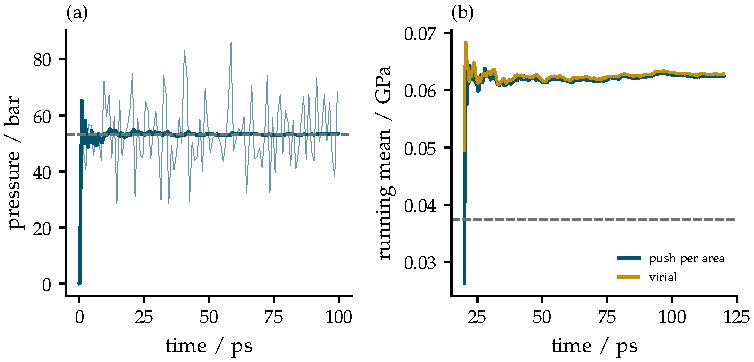
\includegraphics{ch14_pressure/wall}
\caption{Pressure as the push on the walls. (a) 200 argon atoms that do
not interact, in a cube of \SI{40}{\angstrom} between soft walls: the push
per unit area on the six walls, averaged over each picosecond (thin) and
over the run so far (thick), against $N\kB T/V$ (dashed). (b) 256 argon
atoms that interact, in a cube of \SI{23.26}{\angstrom} near
\SI{135}{\kelvin}: the running means of the push per unit area and of the
pressure from the virial, \cref{eq:pr-virial}, against $N\kB T/V$
(dashed).}
\label{fig:pr-wall}
\end{figure}

Atoms that interact push differently. The 256 atoms of the liquid argon
of Chapter~13, held between walls of the same stiffness in a cube of
\SI{23.26}{\angstrom} under CSVR at \SI{135}{\kelvin}, push on the walls
with \SI{0.0624}{\giga\pascal} averaged over \SI{100}{\pico\second} (0.0616
and \SI{0.0633}{\giga\pascal} in the two halves). Their kinetic energy
gives the temperature \SI{133.3}{\kelvin} over the run, a little below the
\SI{135}{\kelvin} the thermostat holds on average, and with it
$N\kB T/V$ is only \SI{0.0374}{\giga\pascal} (\cref{fig:pr-wall}(b)). The atoms
repel one another at close range and the repulsion adds to the push on
the walls. The next section finds by how much.

\begin{keyidea}
Pressure is force per unit area. In a gas it is the momentum the atoms
deliver to the walls per unit time and area, $\sum_im_iv_{ix}^2/V$,
which averages to $N\kB T/V$ for atoms that do not interact. One
\si{\electronvolt\per\angstrom\cubed} is \SI{160.218}{\giga\pascal}, and
\SI{1}{\giga\pascal} is $10^4$ bar.
\end{keyidea}

\notebook{14}{let atoms bounce between walls and read their push}

\begin{selfcheck}
What pressure, in bar, do $10^4$ atoms that do not interact exert at
\SI{300}{\kelvin} in a cube of side \SI{100}{\angstrom}?
\end{selfcheck}

%=============================================================================!
% 14.2  THE VIRIAL                                                            !
%=============================================================================!
\section{The virial}
\label{sec:pr-virial}

Atoms that pull on and push one another deliver momentum to the walls
differently from atoms that only bounce. This section finds the pressure
of interacting atoms from the equipartition theorem applied to their
positions, as Chapter~12 promised, and checks it against the push
measured in \cref{sec:pr-wall}.

\subsection*{Equipartition for positions}

\Cref{eq:sm-equipartition} says that $\ens{x\,\partial H/\partial x} =
\kB T$ for any coordinate $x$ of a system in the canonical ensemble whose
range is closed by a potential that rises without limit, walls included.
For atoms in a box, $H = K + U + U_{\mathrm w}$, with $U$ the energy of
their interactions and $U_{\mathrm w}$ that of the walls. $K$ depends on
the momenta alone, so the slope of $H$ along the coordinate $x_i$ of atom
$i$ is minus the force along it, $\partial H/\partial x_i = -F_{ix} -
F^{\mathrm w}_{ix}$, the first from the other atoms and the second from
the walls. The theorem for $x_i$ then reads $\ens{x_iF_{ix}} +
\ens{x_iF^{\mathrm w}_{ix}} = -\kB T$, and likewise for $y_i$ and $z_i$;
since $x_iF_{ix} + y_iF_{iy} + z_iF_{iz} = \vb{r}_i\cdot\vb{F}_i$, adding
the $3N$ of them gives
\begin{equation*}
   \Bigl\langle\sum_i\vb{r}_i\cdot\vb{F}_i\Bigr\rangle
   + \Bigl\langle\sum_i\vb{r}_i\cdot\vb{F}^{\mathrm w}_i\Bigr\rangle
   = -3N\kB T .
\end{equation*}
The first sum is the virial $\mathcal{W}$ of \cref{sec:pe-forces}, which
for atoms that interact in pairs is $\mathcal{W} = -\sum_{i<j}r_{ij}
\varphi'(r_{ij})$, \cref{eq:pe-virial}: positive when the atoms repel one
another, negative when they attract.

\subsection*{The walls' share}

The second sum comes only from atoms touching a wall. A wall pushes only
at right angles to itself, so an atom touching the wall at $x = L$ has
$\vb{r}_i\cdot\vb{F}^{\mathrm w}_i = x_iF^{\mathrm w}_{ix}$, with $x_i
\approx L$ and the force pointing back into the box; the sum over those
atoms is
\begin{equation*}
   \sum_ix_iF^{\mathrm w}_{ix} \approx L\sum_iF^{\mathrm w}_{ix} =
   -LF_\perp ,
\end{equation*}
with $F_\perp$ the force the atoms exert on the wall, equal and opposite
to the wall's force on them by the third law. On average $F_\perp$ is
$PA$, so this wall contributes $-PAL = -PV$. At the wall $x = 0$ the
atoms have $x_i \approx 0$ and contribute nothing; with the origin at the
centre of the box the two walls share $-PV$ equally instead
(\cref{ex:pr-centre}). The walls normal to $y$ and $z$ do the same, so the
walls' share is $-3PV$. That holds without error for hard walls. An atom
that has gone the depth $\delta$ into a soft wall adds a further
$-k\delta^2$, at $x = 0$ as at $x = L$, so soft walls enlarge the share by
a fraction of about $2\delta/L$. Putting it into the sum,
\begin{equation*}
   \ens{\mathcal{W}} - 3PV = -3N\kB T ,
\end{equation*}
and so
\begin{equation}
   PV = N\kB T + \tfrac13\ens{\mathcal{W}} .
   \label{eq:pr-virial}
\end{equation}
The first term is the ideal gas's, \cref{eq:pr-ideal}; the second is the
interactions' share, raising the pressure when the atoms repel one
another and lowering it when they attract. Since $\ens{2K} = 3N\kB T$ by
equipartition for the momenta, the instantaneous value
\begin{equation*}
   P = \frac{2K + \mathcal{W}}{3V}
\end{equation*}
averages to the pressure, and can be computed at every step from the
positions, velocities and forces the run already has.

\subsection*{Checked}

For the walled liquid of \cref{fig:pr-wall}(b), $(2K + \mathcal{W})/3V$
averages \SI{0.0628}{\giga\pascal} over the run (0.0621 and
\SI{0.0635}{\giga\pascal} in the halves), against \SI{0.0624}{\giga\pascal}
from the push on the walls: the two agree within their scatter. Of the
\SI{0.0628}{\giga\pascal}, \SI{0.0374}{\giga\pascal} is $N\kB T/V$ and
\SI{0.0254}{\giga\pascal} is $\ens{\mathcal{W}}/3V$: at this density the
repulsion between close neighbours outweighs the pull of distant ones.

\begin{keyidea}
Equipartition applied to the positions, $\ens{x\,\partial H/\partial x}
= \kB T$, gives $PV = N\kB T + \frac13\ens{\mathcal{W}}$: the ideal gas's
pressure plus the virial's share, positive for repulsion and negative for
attraction. The instantaneous pressure $(2K + \mathcal{W})/3V$ averages
to it and needs only the positions, velocities and forces.
\end{keyidea}

\begin{selfcheck}
Two argon atoms alone in a box sit \SI{3.0}{\angstrom} apart, closer than
the minimum of the Lennard-Jones potential at $2^{1/6}\sigma =
\SI{3.82}{\angstrom}$. Does their pair raise or lower the pressure from
that of two atoms that do not interact, and why?
\end{selfcheck}

%=============================================================================!
% 14.3  PRESSURE IN A PERIODIC BOX                                            !
%=============================================================================!
\section{Pressure in a periodic box}
\label{sec:pr-periodic}

A periodic box (\cref{sec:md-periodic}) has no walls for its atoms to push
on, and \cref{sec:pr-virial} needed walls. This section finds the
pressure of a periodic box from the free energy, shows that it is
\cref{eq:pr-virial} again with each pair's separation taken to its
nearest copy, and shows what goes wrong when the virial is computed from
the positions instead.

\subsection*{From the free energy}

Chapter~12 found $\dd F = -S\,\dd T - P\,\dd V + \mu\,\dd N$
(\cref{sec:sm-other}), so at fixed $T$ and $N$ the pressure is the rate
at which the free energy falls as the box grows,
\begin{equation*}
   P = -\frac{\partial F}{\partial V} = \kB T\,\frac{\partial\ln
   Z}{\partial V} ,
\end{equation*}
using $F = -\kB T\ln Z$. For a cubic box of side $L$, $V = L^3$, the
partition function is a constant $C$ that depends on $T$ (from the
integral over the momenta) times the integral of $\mathrm{e}^{-\beta U}$
over the positions of every atom inside the box. Writing each position
as $\vb{r}_i = L\vb{s}_i$, with $\vb{s}_i$ the fractional coordinates of
\cref{sec:md-periodic}, each running from 0 to 1, changes the variable of
each of the $3N$ integrals and multiplies it by $L$ (\cref{sec:md-ewald}):
\begin{equation*}
   Z = C\,V^N\int\mathrm{e}^{-\beta U(L\vb{s}_1, \dots, L\vb{s}_N)}\,
   \dd\vb{s}_1\cdots\dd\vb{s}_N .
\end{equation*}
Now the volume appears in two places, $V^N$ and $U$, and the box's
boundaries no longer depend on it. The logarithm is $\ln Z = \ln C +
N\ln V + \ln\int\mathrm{e}^{-\beta U}\,\dd\vb{s}$, with $\dd\vb{s}$ short
for $\dd\vb{s}_1\cdots\dd\vb{s}_N$, and its slope is
\begin{align*}
   \frac{\partial\ln Z}{\partial V}
   &= \frac NV + \frac{\int(-\beta\,\partial U/\partial V)\,
   \mathrm{e}^{-\beta U}\,\dd\vb{s}}{\int\mathrm{e}^{-\beta U}\,\dd\vb{s}}
   && \text{the slope of $\ln$, and the chain rule,}\\
   &= \frac NV - \beta\Bigl\langle\frac{\partial U}{\partial V}\Bigr\rangle
   && \text{a canonical average,}
\end{align*}
with the slope of $U$ taken at fixed fractional coordinates, that is,
with the whole arrangement stretched evenly. For pairs, $U =
\sum_{i<j}\varphi(r_{ij})$, and stretching scales every separation with
the box, $r_{ij} = L\,\lvert\vb{s}_j - \vb{s}_i\rvert$ with the
fractional separation taken to its nearest copy (\cref{sec:md-image}).
So $\partial r_{ij}/\partial L = r_{ij}/L$, and with $\dd L/\dd V =
1/(3L^2)$,
\begin{equation*}
   \frac{\partial U}{\partial V} = \sum_{i<j}\varphi'(r_{ij})\,
   \frac{r_{ij}}{L}\,\frac{1}{3L^2}
   = \frac{1}{3V}\sum_{i<j}r_{ij}\,\varphi'(r_{ij}) = -\frac{\mathcal{W}}{3V} .
\end{equation*}
Then $P = \kB T(N/V - \beta\ens{\partial U/\partial V}) = N\kB T/V +
\ens{\mathcal{W}}/3V$, \cref{eq:pr-virial} again, with $\mathcal{W}$ written
with the separations of \cref{eq:pe-virial}, each to the nearest copy of
the other atom. A periodic run keeps its total momentum at zero, which
removes three of the $3N$ kinetic freedoms, so that $\ens{2K} = (3N -
3)\kB T$ (\cref{sec:sm-equipartition}), and holds its centre of mass
still, so that only $N - 1$ atoms are placed freely and $V^N$ becomes
$V^{N-1}$. The pressure of such a run is $(N - 1)\kB T/V +
\ens{\mathcal{W}}/3V$, one part in $N$ less in its first term, and the
instantaneous $(2K + \mathcal{W})/3V$ averages to it. In
\texttt{md.PairModel} the virial is summed over the pairs of the
neighbour list from their separations, as \cref{sec:pr-tensor} shows,
and \texttt{virial.pressure} adds the kinetic part.

\subsection*{Not from the positions}

The sum $\sum_i\vb{r}_i\cdot\vb{F}_i$ equals \cref{eq:pe-virial} only when,
for every pair, the difference of the positions held, $\vb{r}_j -
\vb{r}_i$, is the separation from which their force was found. Positions
read from the frames of a periodic run are wrapped into the cell
(\cref{sec:md-periodic}): an atom that leaves through one face comes back
through the opposite one, its $\vb{r}_i$ jumping by a lattice vector
while its force does not change. \Cref{sec:pe-forces} showed that moving
the origin by the same vector for every atom leaves $\mathcal{W}$ alone;
wrapping moves single atoms, and changes $\sum_i\vb{r}_i\cdot\vb{F}_i$ by
the scalar product of the lattice vector with that atom's force. Which
atoms have been wrapped depends on where the cell's faces lie, so the sum
depends on where the cell's origin sits. For the liquid of Chapter~13 at
fixed volume, the pressure from the pair separations is
\SI{0.0877}{\giga\pascal}; with $\sum_i\vb{r}_i\cdot\vb{F}_i$ from the
wrapped positions it is \SI{0.0324}{\giga\pascal}, and
\SI{0.0354}{\giga\pascal} with the origin moved, a single frame's value
changing by up to \SI{0.131}{\giga\pascal}. Both lie near the kinetic part
alone, \SI{0.0383}{\giga\pascal}: on average the jumps of the wrapped
atoms cancel the virial's share. Thompson, Plimpton and
Mattson give the general form of the pressure for many-body potentials in
periodic cells, built in the same way from separations\cite{Thompson2009}.

\subsection*{A crystal at rest}

A crystal with every atom on its site has $K = 0$ and its pressure is the
virial's alone. \Cref{fig:pr-crystal}(a) shows it for the face-centred
cubic crystal of the switched Lennard-Jones argon against the cubic
spacing $a$. It is zero at $a_0 = \SI{5.26714}{\angstrom} = 1.54916\sigma$,
the spacing at which \cref{sec:md-start} found the energy least, as it
must be, since $P = -\dd U/\dd V$ at $T = 0$ and the slope of $U$ vanishes
at its least value. A crystal squeezed to $a = \SI{5.20}{\angstrom}$
pushes outwards with \SI{0.128}{\giga\pascal}; one stretched to
\SI{5.40}{\angstrom} pulls inwards with \SI{0.160}{\giga\pascal}, a
negative pressure, a tension. The rise of the pressure for each fraction
by which the volume falls is the bulk modulus,
\begin{equation*}
   B = -V\,\frac{\dd P}{\dd V} = -\frac{\dd P}{\dd V/V} ,
\end{equation*}
the stiffness of the material against squeezing, \SI{2.856}{\giga\pascal}
at $a_0$; its inverse, $\kappa_T = 1/B$ at fixed temperature, is the
compressibility, the fraction by which the volume shrinks for each unit
of pressure.

\begin{figure}[htb]
\centering
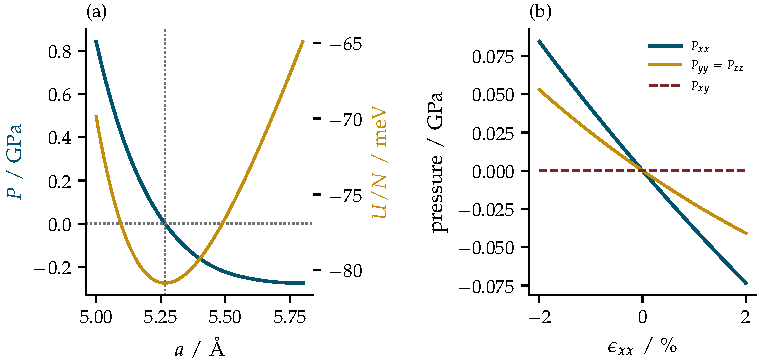
\includegraphics{ch14_pressure/crystal}
\caption{The pressure of the face-centred cubic crystal at rest, 256
atoms of the switched Lennard-Jones argon. (a) The pressure (teal) and the
energy per atom (ochre) against the cubic spacing $a$, the spacing $a_0$
of zero pressure marked (dotted). (b) The crystal at $a_0$ stretched along
$x$ by the strain $\epsilon_{xx}$: the components $\mathsf{P}_{xx}$,
$\mathsf{P}_{yy} = \mathsf{P}_{zz}$ and $\mathsf{P}_{xy}$ (dashed, zero) of the
pressure tensor of \cref{sec:pr-tensor}.}
\label{fig:pr-crystal}
\end{figure}

The liquid of Chapter~13, at \SI{135}{\kelvin} and $0.8\sigma^{-3}$, has
the pressure \SI{0.0877}{\giga\pascal}, about 880 bar, of which
\SI{0.0383}{\giga\pascal} is the kinetic part $2K/3V$. Between walls the
same atoms gave \SI{0.0628}{\giga\pascal} (\cref{sec:pr-virial}): the
walls change the liquid next to them, and only the periodic box gives the
pressure of the liquid far from any wall. For the Lennard-Jones argon with
its energy shifted to zero at \SI{8.5}{\angstrom} in place of the switch,
\texttt{mdlab} and ASE's \texttt{LennardJones} give the same pressure,
\SI{-0.058924}{\giga\pascal}, for a strained crystal of 256 atoms, each
displaced at random by about \SI{0.1}{\angstrom} along each axis.

\begin{keyidea}
In a periodic box $P = -\partial F/\partial V$ gives \cref{eq:pr-virial}
again, with the virial summed over pairs from their separations to the
nearest copy; $\sum_i\vb{r}_i\cdot\vb{F}_i$ from wrapped positions
changes with the origin and is wrong. A crystal at rest has zero
pressure at the spacing of least energy, and its bulk modulus $B =
-V\,\dd P/\dd V$ measures its stiffness against squeezing.
\end{keyidea}

\notebook{14}{shift the origin of a periodic box and watch which pressure changes}

\begin{selfcheck}
From \cref{fig:pr-crystal}(a), the pressure falls from +0.128 to
\SI{-0.160}{\giga\pascal} as $a$ goes from 5.20 to \SI{5.40}{\angstrom}.
Estimate the bulk modulus near $a_0$ from these two points.
\end{selfcheck}

%=============================================================================!
% 14.4  THE PRESSURE TENSOR                                                   !
%=============================================================================!
\section{The pressure tensor}
\label{sec:pr-tensor}

A liquid at rest pushes equally on a face whichever way the face points.
A solid need not: a crystal stretched along $x$ pulls inwards harder on
the faces normal to $x$ than on the others, and a sheet of graphite is
stiff along its plane and soft across it. This section generalises the
pressure to a matrix that gives the push on a face of any orientation.

\subsection*{The push on a face}

The force that the material exerts on a small flat face of area $A$,
whose outward normal is the unit vector $\vb{n}$, need not point along
$\vb{n}$, but it is linear in $\vb{n}$. A small wedge of material cut off
by this face and by three faces normal to the axes, of areas $An_x$,
$An_y$ and $An_z$, feels forces on its faces that shrink with their area,
while its mass shrinks faster, with its volume; as the wedge shrinks the
forces on its four faces must therefore cancel, and the force on the
slanted face is the sum of $An_x$, $An_y$ and $An_z$ times the forces per
unit area on faces normal to $x$, $y$ and $z$. A vector linear in $\vb{n}$
is a matrix times $\vb{n}$ (\cref{sec:os-modes}):
\begin{equation*}
   \vb{F} = A\,\mathsf{P}\vb{n} ,
\end{equation*}
with $\mathsf{P}$ the pressure tensor, whose component
$\mathsf{P}_{\alpha\beta}$ is the force per unit area along $\alpha$ on a
face normal to $\beta$. For a liquid at rest $\mathsf{P} = P\vb{I}$, and
every face is pushed straight outwards with $P$.

\subsection*{From a strain}

\Cref{sec:pr-periodic} stretched the box evenly; stretching it unevenly
gives every component. A small strain multiplies every vector, the
lattice vectors of the cell and the position of every atom alike, by the
matrix $\vb{I} + \boldsymbol{\epsilon}$, with components
$\epsilon_{\alpha\beta}$ that are small. For a cubic cell of side $L$ the
strained lattice vectors are $L$ times the columns $\vb{c}_1$, $\vb{c}_2$
and $\vb{c}_3$ of $\vb{I} + \boldsymbol{\epsilon}$, so by
\cref{eq:md-volume} the volume becomes $V$ times the triple product
$\vb{c}_1\cdot(\vb{c}_2\times\vb{c}_3)$, which is the determinant
$\det(\vb{I} + \boldsymbol{\epsilon})$, the factor by which the strain
stretches volumes (\cref{sec:ha-liouville}). Written out as in
\cref{sec:ro-tensor}, it is six products, each of one component of every
column, and to first order in $\boldsymbol{\epsilon}$
\begin{equation*}
   \det(\vb{I} + \boldsymbol{\epsilon}) = (1 + \epsilon_{xx})(1 +
   \epsilon_{yy})(1 + \epsilon_{zz}) + \dotsb = 1 + \epsilon_{xx} +
   \epsilon_{yy} + \epsilon_{zz} + \dotsb ,
\end{equation*}
since each of the other five products contains at least two off-diagonal
components and is of second order or higher (\cref{ex:pr-det}).

The strain $\dd\epsilon_{\alpha\beta}$ carries the face of a cubic box
normal to $\beta$, at the distance $L$ from the opposite face, a distance
$L\,\dd\epsilon_{\alpha\beta}$ along $\alpha$ further than that opposite
face. The material pushes on the face with $L^2\mathsf{P}_{\alpha\beta}$
along $\alpha$, so it does the work $V\mathsf{P}_{\alpha\beta}\,
\dd\epsilon_{\alpha\beta}$, which its free energy loses at fixed
temperature:
\begin{equation*}
   \dd F = -V\sum_{\alpha\beta}\mathsf{P}_{\alpha\beta}\,
   \dd\epsilon_{\alpha\beta} ,
\end{equation*}
and so $\mathsf{P}_{\alpha\beta} = -(1/V)\,\partial F/\partial
\epsilon_{\alpha\beta}$; an even stretch, $\epsilon_{\alpha\beta} =
e\,\delta_{\alpha\beta}$, changes the volume by $\dd V = 3V\dd e$ and gives
back $\dd F = -P\,\dd V$ with $P$ the mean of the diagonal. The steps of
\cref{sec:pr-periodic} carry over. In fractional coordinates the
partition function carries the factor $\det(\vb{I} +
\boldsymbol{\epsilon})^N$, whose logarithm, $N\ln(1 + \epsilon_{xx} +
\epsilon_{yy} + \epsilon_{zz} + \dotsb)$, has the slope
$N\delta_{\alpha\beta}$ along $\epsilon_{\alpha\beta}$ at zero strain. Each
pair separation $\vb{d}$, of length $r_{ij}$, becomes $(\vb{I} +
\boldsymbol{\epsilon})\vb{d}$, with components $d_\alpha +
\sum_\beta\epsilon_{\alpha\beta}d_\beta$; squaring and adding them, and
dropping the products of two strains, gives the squared length $r_{ij}^2 +
2\sum_{\alpha\beta}d_\alpha\epsilon_{\alpha\beta}d_\beta$, and since
$\sqrt{r^2 + x} \approx r + x/2r$ for small $x$ (\cref{sec:mo-taylor}),
the length grows by $\sum_{\alpha\beta}d_\alpha\epsilon_{\alpha\beta}
d_\beta/r_{ij}$. Its slope along $\epsilon_{\alpha\beta}$ is $d_\alpha
d_\beta/r_{ij}$, and by the chain rule
\begin{equation*}
   \frac{\partial U}{\partial\epsilon_{\alpha\beta}}
   = \sum_{i<j}\varphi'(r_{ij})\,\frac{d_\alpha d_\beta}{r_{ij}}
   = -\mathcal{W}_{\alpha\beta} ,
\end{equation*}
with $\mathcal{W}_{\alpha\beta}$ the virial tensor, whose trace, the sum of
its diagonal, is $\mathcal{W}$. Then, as in \cref{sec:pr-periodic},
\begin{equation*}
   \mathsf{P}_{\alpha\beta} = \frac{\kB T}{V}\,
   \frac{\partial\ln Z}{\partial\epsilon_{\alpha\beta}}
   = \frac1V\bigl(N\kB T\,\delta_{\alpha\beta}
   + \ens{\mathcal{W}_{\alpha\beta}}\bigr) .
\end{equation*}
Equipartition gives $\ens{m_iv_{i\alpha}^2} = \kB T$, and in the Maxwell
distribution (\cref{sec:sm-maxwell}) the components of a velocity are
independent with mean zero, so $\ens{m_iv_{i\alpha}v_{i\beta}} = \kB T\,
\delta_{\alpha\beta}$, and the instantaneous
\begin{equation}
   \mathsf{P}_{\alpha\beta} = \frac1V\Bigl(\sum_im_iv_{i\alpha}v_{i\beta}
   + \mathcal{W}_{\alpha\beta}\Bigr)
   \label{eq:pr-tensor}
\end{equation}
averages to the pressure tensor, and the mean of its diagonal is the
instantaneous pressure of \cref{sec:pr-virial}. \texttt{md.PairModel}
stores $\mathcal{W}_{\alpha\beta}$ at every call, from the separations
$\vb{d}$ of the pairs and the forces between them:

\begin{code}
        r = np.asarray(positions, dtype=float)
        i, j, d, dist = self.neighbours.pairs(r)
        phi, dphi = self._pair(i, j, dist)
        push = (dphi / dist)[:, None] * d  # the force on i from j
        forces = np.zeros_like(r)
        np.add.at(forces, i, push)
        np.add.at(forces, j, -push)
        self.virial = -np.einsum("pa,pb->ab", d, push)
        return float(np.sum(phi)), forces
\end{code}

\noindent \texttt{d} holds $\vb{r}_j - \vb{r}_i$ to the nearest copy and
\texttt{push} the force on $i$ from $j$, $\varphi'(r_{ij})\,\vb{d}/r_{ij}$
(\cref{sec:pe-forces}), so \texttt{virial} is $-\sum d_\alpha F_\beta =
-\sum\varphi'(r_{ij})\,d_\alpha d_\beta/r_{ij}$ over the pairs,
$\mathcal{W}_{\alpha\beta}$. It agrees with $-\partial U/\partial
\epsilon_{\alpha\beta}$ for each of the nine strains, taken by finite
differences, to \SI{2.1e-9}{\electronvolt}, and $-\mathcal{W}_{\alpha\beta}
/V$ agrees with the stress of ASE's \texttt{LennardJones} to
\SI{7.5e-16}{\giga\pascal}.

\subsection*{Measured}

The liquid's tensor is isotropic: under the cell rescaling of
\cref{sec:pr-rescaling} at \SI{0.1}{\giga\pascal} its diagonal averages
0.1003, 0.0995 and \SI{0.0996}{\giga\pascal} and its off-diagonal
components $-0.0002$, 0.0000 and \SI{-0.0001}{\giga\pascal}, while an
instantaneous diagonal component scatters by \SI{0.023}{\giga\pascal} and
an off-diagonal one by \SI{0.013}{\giga\pascal}. The crystal at $a_0$
stretched along $x$ is not (\cref{fig:pr-crystal}(b)): at
$\epsilon_{xx} = +0.02$, $\mathsf{P}_{xx} = \SI{-0.0735}{\giga\pascal}$ while
$\mathsf{P}_{yy} = \mathsf{P}_{zz} = \SI{-0.0409}{\giga\pascal}$, and the
off-diagonal components stay at zero. The slopes at zero strain are the
crystal's elastic stiffnesses, $C_{11} = -\partial\mathsf{P}_{xx}/\partial
\epsilon_{xx} = \SI{3.920}{\giga\pascal}$ and $C_{12} = -\partial
\mathsf{P}_{yy}/\partial\epsilon_{xx} = \SI{2.324}{\giga\pascal}$. An even
squeeze applies all three strains at once; by the cubic symmetry
$\mathsf{P}_{xx}$ responds to $\epsilon_{yy}$ and $\epsilon_{zz}$ as
$\mathsf{P}_{yy}$ does to $\epsilon_{xx}$, so each diagonal component
changes by $-(C_{11} + 2C_{12})e$ while $\dd V/V = 3e$, and the bulk
modulus is $(C_{11} + 2C_{12})/3 = \SI{2.856}{\giga\pascal}$, the value
\cref{sec:pr-periodic} found from the slope of $P$.

ASE, like many libraries, reports the stress, which is $-\mathsf{P}$,
positive when the material is pulled; a program's sign convention is
worth checking before its numbers are used. ASE's \texttt{get\_stress}
returns it in \si{\electronvolt\per\angstrom\cubed} as six numbers,
\begin{equation*}
   -\mathsf{P}_{xx},\ -\mathsf{P}_{yy},\ -\mathsf{P}_{zz},\
   -\mathsf{P}_{yz},\ -\mathsf{P}_{xz},\ -\mathsf{P}_{xy} ,
\end{equation*}
and leaves out the kinetic part unless
it is called with \texttt{include\_ideal\_gas=True}; the pressure is then
minus the mean of the first three.

\begin{bridge}
In a density-functional calculation the stress is the same derivative of
the energy with respect to strain, and Nielsen and Martin showed how to
compute it from the electronic structure directly\cite{Nielsen1985}. A
basis of plane waves cut off at a fixed energy changes when the cell
does, so a cell that grows during a calculation is described by a basis
of different quality from the one it started with, and the stress
carries a spurious part, the Pulay stress; it is removed by raising the
cutoff until the stress no longer changes, or by correcting for the
incomplete basis as Francis and Payne set out\cite{Francis1990}. A basis
of orbitals centred on the atoms moves with them instead, and its
derivatives enter the stress as Pulay terms, as they enter the forces
(\cref{sec:en-atoms}).
\end{bridge}

\begin{keyidea}
The pressure tensor gives the force per unit area on a face of any
orientation, $\vb{F} = A\,\mathsf{P}\vb{n}$; it is $(\sum m v_\alpha v_\beta
+ \mathcal{W}_{\alpha\beta})/V$, from the response of the free energy to a
strain, and the mean of its diagonal is the pressure. A liquid's is $P$
times the unit matrix; a strained crystal's is not. Libraries report the
stress, $-\mathsf{P}$.
\end{keyidea}

\notebook{14}{stretch the crystal along one axis and read the tensor}

\begin{selfcheck}
ASE's stress, with the kinetic part included, is
\SI{0.002}{\electronvolt\per\angstrom\cubed} for each of its first three
numbers and zero for the others. What is the pressure in GPa, and is the
material pushing on its cell or pulling on it?
\end{selfcheck}

%=============================================================================!
% 14.5  WHAT A BAROSTAT MUST DO                                               !
%=============================================================================!
\section{What a barostat must do}
\label{sec:pr-npt}

A barostat lets the volume of the box change so that the run samples the
ensemble at constant pressure. This section sets out what that ensemble
requires, finds the exact distribution of the volume for an ideal gas and
its spread for a liquid, which are the tests every barostat of the
chapter must pass, and fits a barostat into the loop of Chapter~13.

\subsection*{The ensemble at constant pressure}

A system that exchanges volume with a bath at the pressure $P_0$ has the
weight $\mathrm{e}^{-\beta(H + P_0V)}$ (\cref{sec:sm-other}). Grouping the
states by their volume gives the probability of each volume,
\begin{equation*}
   \mathcal{P}(V) \propto \mathrm{e}^{-\beta P_0V}\,Z(N, V, T) ,
\end{equation*}
the canonical partition function of the box at that volume weighted by
$\mathrm{e}^{-\beta P_0V}$. A barostat must therefore do two things that a
thermostat does not: move the volume, and move it so that it takes each
value with this probability. Its mean pressure should be $P_0$, and the
spread of its volume should be the one this distribution has.

\subsection*{The ideal gas exactly}

For atoms that do not interact, $U = 0$ and \cref{sec:pr-periodic} gives
$Z = C\,V^N$, so
\begin{equation*}
   \mathcal{P}(V) \propto V^N\mathrm{e}^{-bV} , \qquad b = \frac{P_0}{\kB T} .
\end{equation*}
The integrals $\int_0^\infty V^n\mathrm{e}^{-bV}\dd V = n!/b^{n+1}$, found by
integrating by parts $n$ times (\cref{ex:pr-gamma}), give the mean and the
variance, each the integral with one or two more powers of $V$ divided by
the integral with none:
\begin{align*}
   \ens{V} &= \frac{(N + 1)!/b^{N+2}}{N!/b^{N+1}} = \frac{N + 1}{b}
   = \frac{(N + 1)\kB T}{P_0} ,\\
   \ens{V^2} &= \frac{(N + 2)!/b^{N+3}}{N!/b^{N+1}}
   = \frac{(N + 2)(N + 1)}{b^2} , \qquad
   \ens{V^2} - \ens{V}^2 = \frac{N + 1}{b^2} .
\end{align*}
The mean is the ideal gas law's with $N + 1$ in place of $N$, a difference
that vanishes for large $N$, and the relative spread is $1/\sqrt{N + 1}$.
For 20 atoms at \SI{135}{\kelvin} and $P_0 = \SI{1e-4}{\electronvolt\per
\angstrom\cubed}$, the mean volume is \SI{2443}{\angstrom\cubed} and its
spread \SI{533}{\angstrom\cubed}: a small gas whose volume fluctuates by a
fifth, a severe test (\texttt{virial.ideal\_gas\_volume\_density} gives
the whole density).

\subsection*{A liquid's volume}

Chapter~12 found that the volume at constant pressure fluctuates with the
variance $-\kB T\,\dd\ens{V}/\dd P$ (\cref{ex:sm-volume}). With the
compressibility of \cref{sec:pr-periodic}, $\dd\ens{V}/\dd P =
-\ens{V}\kappa_T$, so
\begin{equation}
   \ens{V^2} - \ens{V}^2 = \kB T\,\ens{V}\,\kappa_T .
   \label{eq:pr-volume}
\end{equation}
A soft material swings its volume more than a stiff one. To test a
barostat on the liquid this needs $\kappa_T$ found without one. Three
runs at fixed volume around the volume the liquid takes at
\SI{0.1}{\giga\pascal}, three starts each of \SI{100}{\pico\second} under
CSVR at \SI{135}{\kelvin}, give
\begin{center}
\small
\begin{tabular}{@{}lccc@{}}
\toprule
$V$ / \si{\angstrom\cubed} & 12\,112 & 12\,301 & 12\,477\\
$\ens{P}$ / \si{\giga\pascal} & $0.1109 \pm 0.0004$ & $0.1000 \pm 0.0005$
   & $0.0904 \pm 0.0013$\\
\bottomrule
\end{tabular}
\end{center}
with the standard error of the three starts. The parabola through the
three points has, at \SI{12306}{\angstrom\cubed}, the mean volume of the
runs at constant pressure of \cref{sec:pr-rescaling,sec:pr-piston}, the
slope $\dd P/\dd V$ that gives $\kappa_T = -1/(V\,\dd P/\dd V) = (1.46 \pm
0.11)$\,\si{\per\giga\pascal}, the error found by redrawing the three
pressures within their standard errors; the liquid's bulk modulus is a
quarter of the crystal's. \Cref{eq:pr-volume} then predicts a spread of
\SI{183}{\angstrom\cubed}, 1.5\% of the volume.

\subsection*{The barostat in the loop}

\texttt{barostats.run} is Chapter~13's loop with one addition. At the
start of each step, after the thermostat has acted, the barostat reads
the instantaneous pressure tensor, \cref{eq:pr-tensor}, from the
velocities and the virial the last force call left, and changes the cell,
scaling the positions with it so that their fractional coordinates are
kept, and, for some barostats, the velocities; the forces are then
computed again in the new cell and the step continues as velocity
Verlet. The neighbour list is kept across such changes while no pair can
have been missed. If the strain since the list was built stretches or
shrinks no separation by more than the fraction $e$ of its length (for a
box scaled by the factor $1 + e$ along every edge, $e$ itself), and no atom
has moved further than $u$ from where the strain alone would have carried
it, a pair now within $r_{\mathrm c}$ was within $r_{\mathrm c} + 2u$ after
the strain alone, and so within $(r_{\mathrm c} + 2u)/(1 - e)$ when the
list was built. The list of \cref{sec:md-neighbours} therefore holds while
$(r_{\mathrm c} + 2u)/(1 - e) \le r_{\mathrm c} + r_{\mathrm{skin}}$; with the
box fixed, $e = 0$ and this is the rule $u \le \frac12r_{\mathrm{skin}}$ of
that section. The run records the work, the change of
$K + U + P_0V$ that the barostat makes, beside the heat of the
thermostat; the effective energy $K + U + P_0V$ less the heat and the work
changes only through the integration error, as \cref{eq:th-effective} did
for a thermostat.

\begin{keyidea}
A barostat must sample $\mathcal{P}(V) \propto \mathrm{e}^{-\beta
P_0V}Z(N, V, T)$: the mean pressure $P_0$, and the right spread of volume.
For an ideal gas $\mathcal{P}(V) \propto V^N\mathrm{e}^{-\beta P_0V}$, with
mean $(N + 1)\kB T/P_0$ and relative spread $1/\sqrt{N + 1}$; for a liquid
the variance of $V$ is $\kB T\ens{V}\kappa_T$, with $\kappa_T$ measured at
fixed volumes.
\end{keyidea}

\begin{selfcheck}
By what fraction does the volume of 1000 ideal-gas atoms fluctuate at
constant pressure?
\end{selfcheck}

%=============================================================================!
% 14.6  WEAK COUPLING AND STOCHASTIC CELL RESCALING                           !
%=============================================================================!
\section{Weak coupling and stochastic cell rescaling}
\label{sec:pr-rescaling}

Chapter~13 built weak coupling for the temperature, found its
fluctuations too narrow, and mended it with noise. The same two steps
give the two first-order barostats of this section, which set the rate of
change of the volume directly, with no momentum of the volume to carry
it on: Berendsen's, which
relaxes the pressure towards its target, and stochastic cell rescaling,
which adds the noise that gives the volume its right spread.

\subsection*{Weak coupling}

Berendsen and colleagues asked the pressure to relax towards $P_0$ with a
time constant $\tau_{\mathrm P}$\cite{Berendsen1984},
\begin{equation*}
   \frac{\dd P}{\dd t} = \frac{P_0 - P}{\tau_{\mathrm P}} .
\end{equation*}
The pressure responds to the volume through the compressibility, $\dd P
= -\dd V/(V\kappa)$, with $\kappa$ an estimate of the material's
$\kappa_T$, so the volume must change at the rate
\begin{equation*}
   \frac{\dd V}{\dd t} = -V\kappa\,\frac{\dd P}{\dd t}
   = -\frac{V\kappa}{\tau_{\mathrm P}}(P_0 - P) .
\end{equation*}
Over one step $\dt$ the volume is multiplied by $1 -
(\kappa\dt/\tau_{\mathrm P})(P_0 - P)$, and each length by its cube root,
which to first order in the small change, by $(1 + y)^{1/3} \approx 1 +
y/3$ from the Taylor series of \cref{sec:mo-taylor}, is
\begin{equation*}
   1 - \frac{\kappa\dt}{3\tau_{\mathrm P}}(P_0 - P) ;
\end{equation*}
\texttt{barostats.Berendsen} scales the cell and the positions by this
factor at the start of each step, leaving the velocities as they are, and
with Berendsen's thermostat follows ASE's \texttt{NPTBerendsen} to
\SI{7.9e-8}{\angstrom} over 40 steps. The estimate $\kappa$ need not be
right. Near the mean volume $\bar V$, $P_0 - P \approx (V - \bar
V)/(\bar V\kappa_T)$ with the true $\kappa_T$, so
\begin{equation*}
   \frac{\dd V}{\dd t} = -\frac{\kappa}{\kappa_T\tau_{\mathrm P}}(V - \bar V) ,
\end{equation*}
and the volume relaxes with the time constant $\tau_{\mathrm P}\kappa_T/
\kappa$, in the way the gap $w$ of \cref{sec:ne-drag} did: a wrong
$\kappa$ changes only how fast the volume settles. We gave the
barostats on the liquid the rough guess $\kappa = \SI{2.5}{\per\giga
\pascal}$; with the measured $\kappa_T = \SI{1.46}{\per\giga\pascal}$ and
$\tau_{\mathrm P} = \SI{1}{\pico\second}$ the liquid's volume relaxes in
\SI{0.58}{\pico\second}.

Like its thermostat, Berendsen's barostat holds the mean pressure and
squeezes the fluctuations (\cref{fig:pr-volume}). On the ideal gas of
\cref{sec:pr-npt}, under Langevin friction, which leaves all $3N$ momenta
free so that $\ens{2K} = 3N\kB T$, its volume spreads by
\SI{192}{\angstrom\cubed}, 0.361 of the exact \SI{533}{\angstrom\cubed},
and even its mean is off, \SI{2328}{\angstrom\cubed} against
\SI{2443}{\angstrom\cubed}. The barostat and the ensemble both hold the
mean of the instantaneous pressure, here $2K/3V$, at $P_0$, which fixes
$\ens{1/V} = P_0/N\kB T$. The ensemble's wide spread makes $\ens{1/V}$
larger than $1/\ens{V}$, by the factor $(N + 1)/N$, which puts its mean at
$(N + 1)\kB T/P_0$; Berendsen's narrow spread leaves $\ens{1/V}$ close to
$1/\ens{V}$ and the volume near $N\kB T/P_0 = \SI{2327}{\angstrom\cubed}$
(\cref{ex:pr-berendsen-mean}). On the liquid, with three runs
of \SI{300}{\pico\second} at \SI{0.1}{\giga\pascal} and \SI{135}{\kelvin}
under CSVR, the mean pressure is \SI{0.1000}{\giga\pascal}, but
$\kappa_T$ read from the volume's fluctuations by \cref{eq:pr-volume} is
$(0.64 \pm 0.05)$\,\si{\per\giga\pascal} against the
\SI{1.46}{\per\giga\pascal} measured at fixed volumes.

\begin{figure}[htb]
\centering
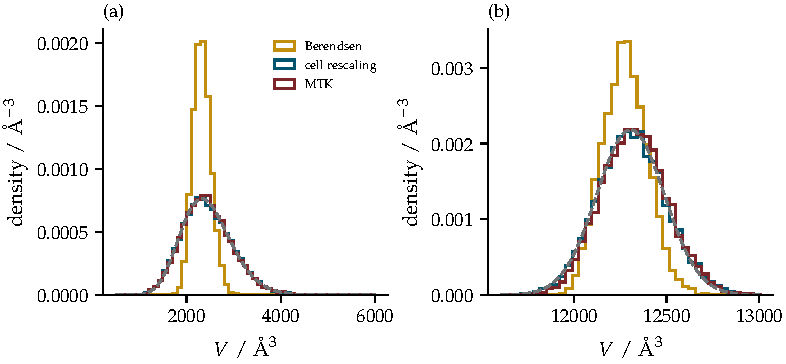
\includegraphics{ch14_pressure/volume}
\caption{The volume a barostat samples. (a) 20 argon atoms that do not
interact, at \SI{135}{\kelvin} and $P_0 = \SI{1e-4}{\electronvolt\per
\angstrom\cubed}$, with $\tau_{\mathrm P} = \SI{0.2}{\pico\second}$, and
$\kappa = 1/P_0$ and Langevin friction for the first-order barostats: the
density of the volume under Berendsen's barostat, stochastic cell
rescaling and the piston of Martyna, Tobias and Klein (MTK) of
\cref{sec:pr-piston} with its chains,
against the exact $V^N\mathrm{e}^{-\beta P_0V}$ (dashed). (b) The liquid
at \SI{135}{\kelvin} and \SI{0.1}{\giga\pascal}, three runs of
\SI{300}{\pico\second} for each: the density of the volume, against the
Gaussian of variance $\kB T\ens{V}\kappa_T$ with $\kappa_T$ from the
runs at fixed volume (dashed).}
\label{fig:pr-volume}
\end{figure}

\subsection*{Noise for the volume}

Bernetti and Bussi mended the barostat as CSVR mended the
thermostat\cite{Bernetti2020}. Berendsen's drift, written for $\ln V$, is
$\dd\ln V = \dd V/V = -(\kappa/\tau_{\mathrm P})(P_0 - P)\,\dd t$. Near the
mean, $\ln V - \ln\bar V \approx (V - \bar V)/\bar V$, so $P_0 - P \approx
(\ln V - \ln\bar V)/\kappa_T$ and
\begin{equation*}
   \dd\ln V = -\frac{\kappa}{\kappa_T\tau_{\mathrm P}}\,(\ln V - \ln\bar V)
   \,\dd t ,
\end{equation*}
the drag of \cref{sec:th-langevin} with $\gamma = \kappa/(\kappa_T
\tau_{\mathrm P})$, acting on $\ln V - \ln\bar V$. Adding kicks of strength
$\sigma$ makes it the Ornstein-Uhlenbeck process of \cref{eq:th-ou},
whose variance settles at $\sigma^2/2\gamma$ (\cref{ex:th-ou-variance}).
The ensemble asks for the variance of $\ln V$ to be that of $V$ over
$\bar V^2$, $\kB T\kappa_T/\bar V$ by \cref{eq:pr-volume}, so
\begin{equation*}
   \frac{\sigma^2}{2\gamma} = \frac{\kB T\kappa_T}{\bar V}
   \quad\Longrightarrow\quad
   \sigma^2 = \frac{2\kappa}{\kappa_T\tau_{\mathrm P}}\,
   \frac{\kB T\kappa_T}{\bar V} = \frac{2\kB T\kappa}{\bar V\tau_{\mathrm P}} ,
\end{equation*}
and the unknown $\kappa_T$ cancels. Stochastic cell rescaling keeps this
noise, with the current $V$ in place of $\bar V$:
\begin{equation}
   \dd\ln V = -\frac{\kappa}{\tau_{\mathrm P}}(P_0 - P)\,\dd t
   + \sqrt{\frac{2\kB T\kappa\,\dd t}{V\tau_{\mathrm P}}}\;g ,
   \label{eq:pr-scr}
\end{equation}
with $g$ a fresh number from the normal distribution of mean 0 and
variance 1 at each interval $\dd t$, the kick of \cref{sec:th-langevin}:
the fluctuation-dissipation relation again, now for the volume. Bernetti
and Bussi showed that it samples the ensemble at constant pressure far
from the mean as well as near it\cite{Bernetti2020}, provided $P$ is the
instantaneous pressure taken along the path on which the barostat moves
the atoms. Their drift comes from the slope of $K + U + P_0V$ with $V$
along that path, so $P$ must be $-\partial(K + U)/\partial V$ there. The
virial part already is, since \cref{sec:pr-periodic} took $\partial U/
\partial V$ at fixed fractional coordinates. If every momentum is scaled by
$V^{-1/3}$ as the box grows, $K \propto V^{-2/3}$ and $\partial K/\partial V
= -\frac23K/V$ (\cref{ex:pr-kinetic}), so $-\partial K/\partial V$ is $2K/3V$,
the kinetic part of the instantaneous pressure. Each length is therefore
multiplied by $\mathrm{e}^{\dd\ln V/3}$ and each velocity by
$\mathrm{e}^{-\dd\ln V/3}$. \texttt{StochasticCellRescaling.scale} takes
one such step of \cref{eq:pr-scr} each time step:

\begin{code}
        kappa, tau, p0 = self.compressibility, self.tau, self.pressure
        kt_v = self.kb * self.temperature / cell_volume(h)
        diagonal = np.diag(tensor)
        if self.couple == "isotropic":
            d_log_v = (-kappa / tau * (p0 - diagonal.mean()) * dt
                       + math.sqrt(2 * kt_v * kappa * dt / tau)
                       * rng.standard_normal())
            stretch = np.full(3, math.exp(d_log_v / 3))
\end{code}

\noindent followed by \texttt{\_scale\_cell}, which multiplies the cell's
lattice vectors by \texttt{stretch}, the positions with them, and the
velocities by the inverse. For the liquid, a step moves $\ln V$ by noise
of spread $2.75\times10^{-3}$, against its settled spread of 0.0149.

\subsection*{Measured}

On the ideal gas the volume now follows the exact density closely
(\cref{fig:pr-volume}(a)): mean \SI{2444}{\angstrom\cubed}, 1.000 of the
exact, and spread \SI{541}{\angstrom\cubed}, 1.014 of it. On the liquid
the three runs give $\kappa_T = (1.50 \pm 0.05)$\,\si{\per\giga\pascal}
from the fluctuations, against \SI{1.46}{\per\giga\pascal} at fixed
volumes, with the mean pressure 0.0988, 0.1004 and
\SI{0.1002}{\giga\pascal}. ASE has no stochastic cell rescaling; the
ideal gas, whose answer is known exactly, is the independent check.

\begin{keyidea}
Berendsen's barostat scales each length by $1 - (\kappa\dt/3\tau_{\mathrm
P})(P_0 - P)$: it holds the mean pressure, relaxes the volume in
$\tau_{\mathrm P}\kappa_T/\kappa$, and squeezes the volume's fluctuations,
to 0.36 of the exact spread for a small ideal gas and to less than half
the compressibility for the liquid. Stochastic cell rescaling adds to $\ln V$
the noise $\sqrt{2\kB T\kappa\,\dd t/(V\tau_{\mathrm P})}\,g$ that the
fluctuation-dissipation relation demands, and samples the volume
correctly.
\end{keyidea}

\notebook{14}{set the barostat's time constant and compare the volume with the exact density}

\begin{selfcheck}
The liquid reads \SI{0.08}{\giga\pascal} with the target
\SI{0.1}{\giga\pascal}, $\kappa = \SI{2.5}{\per\giga\pascal}$ and
$\dt/\tau_{\mathrm P} = 0.01$. By what factor does Berendsen's barostat
multiply each length in this step?
\end{selfcheck}

%=============================================================================!
% 14.7  A PISTON WITH MASS                                                    !
%=============================================================================!
\section{A piston with mass}
\label{sec:pr-piston}

The barostats of \cref{sec:pr-rescaling} move the volume as a heavily
damped quantity, with no momentum of its own. A real piston has mass: it
overshoots and swings. This section builds the barostat that treats the
volume as a coordinate with inertia, finds the frequency at which it
swings, and measures it.

\subsection*{A piston on a gas spring}

A piston of mass $M_{\mathrm p}$ and area $A$ rests on a column of gas of
height $x$, so $V = Ax$, with the pressure $P_0$ above it. The gas pushes
up with $PA$ and the outside pushes down with $P_0A$, so $M_{\mathrm
p}\ddot x = A(P - P_0)$. If the piston is moved by $\delta x$ from where
the two balance, the volume changes by $A\,\delta x$ and the gas's
pressure by $\delta P = -A\,\delta x/(V\kappa)$, and
\begin{equation*}
   M_{\mathrm p}\,\ddot{\delta x} = -\frac{A^2}{V\kappa}\,\delta x :
\end{equation*}
the oscillator of \cref{sec:os-small}, with the gas as its spring, of
stiffness $A^2/V\kappa$, and the frequency $\omega^2 = A^2/(M_{\mathrm
p}V\kappa)$. A heavy piston on a soft gas swings slowly.

\subsection*{The volume as a coordinate}

Andersen turned this into a barostat\cite{Andersen1980}: the volume is
given a mass and a kinetic energy of its own, the outside does the work
$P_0V$, and the atoms' positions scale with the box, so that the volume
accelerates in proportion to $P - P_0$ and the sum of $H$, $P_0V$ and the
piston's kinetic energy is kept. The form of Martyna, Tobias and Klein
(MTK)\cite{Martyna1994}, which ASE and \texttt{mdlab} follow, takes as its coordinate the strain $\epsilon$
by which every length is $\mathrm{e}^\epsilon$ times its starting value, so
$V = V_0\mathrm{e}^{3\epsilon}$, with the momentum $p_\epsilon$ and the
mass $M_\epsilon$. Its equations are
\begin{align*}
   \dot{\vb{r}}_i &= \vb{v}_i + \frac{p_\epsilon}{M_\epsilon}\vb{r}_i ,
   & m_i\dot{\vb{v}}_i &= \vb{F}_i - \Bigl(1 + \frac{3}{N_{\mathrm f}}\Bigr)
   \frac{p_\epsilon}{M_\epsilon}m_i\vb{v}_i ,\\
   \dot V &= \frac{3Vp_\epsilon}{M_\epsilon} ,
   & \dot p_\epsilon &= 3V(P - P_0) + \frac{3}{N_{\mathrm f}}\sum_im_iv_i^2 ,
\end{align*}
with $N_{\mathrm f}$ the number of free momenta. Here $\vb{v}_i =
\vb{p}_i/m_i$ is the velocity of atom $i$ relative to the stretching box,
which the first equation adds to the box's own motion to give
$\dot{\vb{r}}_i$, and $P$ is the instantaneous pressure computed with
these $\vb{v}_i$. The first equation carries each atom along as the box
grows, the second slows the atoms as it does, the third ties the volume
to the strain, and the fourth pushes the piston with the difference of
pressures. Martyna, Tobias and Klein showed that with the two terms in
$3/N_{\mathrm f}$ these equations, given a thermostat, sample the ensemble
at constant pressure; without them the distribution of the volume is
wrong by an amount that shrinks as $N$ grows. Nosé-Hoover chains
(\cref{sec:th-nose}) add a friction to the second and fourth equations,
acting on the atoms and on $p_\epsilon$, and the run keeps $K + U + P_0V +
p_\epsilon^2/2M_\epsilon$ plus the chains' energies.
\texttt{barostats.run\_mtk} integrates these equations by the Trotter
splitting (\cref{sec:in-splitting}) of Tuckerman and
colleagues\cite{Tuckerman2006}, as ASE's
\texttt{IsotropicMTKNPT} does, and follows it to \SI{5.6e-7}{\angstrom}
over 40 steps. Both take $N_{\mathrm f} = 3N$. A liquid whose total
momentum stays at zero has only $3N - 3$ free momenta, and with $3N$ in
the chain its kinetic temperature runs high by about $3/(3N - 3)$, 0.4\%
for 256 atoms: the three runs of \cref{fig:pr-volume}(b) average 135.48,
135.99 and \SI{135.94}{\kelvin} against the \SI{135}{\kelvin} asked
for.

\subsection*{How fast it swings}

Ignoring the chains and the term $(3/N_{\mathrm f})\sum_im_iv_i^2$, which
stays close to $3\kB T$ and only shifts where the piston balances,
$M_\epsilon\ddot\epsilon = 3V(P - P_0)$. A change of the strain by
$\delta\epsilon$ changes the volume by $3V\delta\epsilon$ and, taking the
response at fixed temperature, the pressure by $\delta P =
-3\delta\epsilon/\kappa_T$, so
\begin{equation*}
   M_\epsilon\,\ddot{\delta\epsilon} = -\frac{9V}{\kappa_T}\,\delta\epsilon ,
   \qquad \omega^2 = \frac{9V}{M_\epsilon\kappa_T} ,
\end{equation*}
the piston on its gas spring again. ASE and \texttt{mdlab} take the mass
from a time constant, $M_\epsilon = (3N + 3)\kB T\tau_{\mathrm P}^2$, which
gives the period (\cref{ex:pr-period})
\begin{equation*}
   \frac{2\pi}{\omega} = 2\pi\tau_{\mathrm P}\sqrt{\frac{(N + 1)\kB T
   \kappa_T}{3V}} ;
\end{equation*}
for the liquid, with $\kappa_T = \SI{1.46}{\per\giga\pascal}$, it is
$0.865\,\tau_{\mathrm P}$, and $M_\epsilon = \SI{8.97e6}{\electronvolt\femto
\second\squared}$ for $\tau_{\mathrm P} = \SI{1}{\pico\second}$. Measured
from the crossings of the volume through its mean
(\cref{fig:pr-piston}), the periods are 0.248, 0.876, 2.450 and
\SI{8.695}{\pico\second} for $\tau_{\mathrm P}$ of 0.3, 1, 3 and
\SI{10}{\pico\second}, against 0.259, 0.865, 2.594 and
\SI{8.647}{\pico\second} predicted, the agreement within 6\% bearing out
the response taken at fixed temperature.

\begin{figure}[htb]
\centering
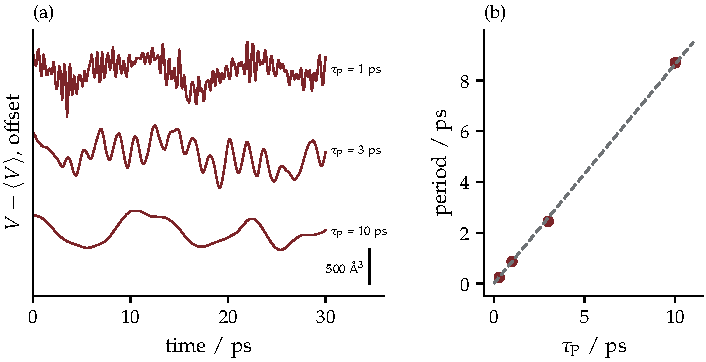
\includegraphics{ch14_pressure/piston}
\caption{A piston with mass rings. The liquid at \SI{135}{\kelvin} and
\SI{0.1}{\giga\pascal} under the MTK piston with chains. (a) The volume's
departure from its mean over the first \SI{30}{\pico\second} for
$\tau_{\mathrm P} = 1$, 3 and \SI{10}{\pico\second}, each trace offset by
\SI{1200}{\angstrom\cubed}. (b) The period of the volume's swing against
$\tau_{\mathrm P}$ (points) and the period of the linearised piston
(dashed).}
\label{fig:pr-piston}
\end{figure}

The piston samples the right volume (\cref{fig:pr-volume}): on the ideal
gas its mean is 0.999 and its spread 0.994 of the exact values, and on
the liquid, with $\tau_{\mathrm P} = \SI{1}{\pico\second}$, the volume's
fluctuations give $\kappa_T = (1.39 \pm 0.06)$\,\si{\per\giga\pascal}
against \SI{1.46}{\per\giga\pascal}. How heavy the piston should be is a
question of time. With $\tau_{\mathrm P} = \SI{10}{\pico\second}$ the
volume swings only 10 times in \SI{90}{\pico\second}, too few for a run of
that length to average its swings away; with \SI{1}{\pico\second} it
swings 103 times.

\subsection*{Changing shape}

Parrinello and Rahman gave every component of the cell matrix $\vb{h}$ a
mass and a momentum, so that the cell can change its shape as well as its
size, each lattice vector a piston of its own, and used it to follow a
crystal from one structure to another\cite{Parrinello1981}. Martyna,
Tobias and Klein gave the same freedom to their piston. \texttt{mdlab}
has only the isotropic piston; \cref{sec:pr-shape} changes the shape of
the cell with first-order barostats instead.

\begin{keyidea}
A piston with mass treats the volume as a coordinate pushed by $P -
P_0$; it swings like a mass on a gas spring, with $\omega^2 = 9V/(M_\epsilon
\kappa_T)$, a period of $0.865\,\tau_{\mathrm P}$ for the liquid with the
mass $(3N + 3)\kB T\tau_{\mathrm P}^2$. With Nosé-Hoover chains and the
corrections of Martyna, Tobias and Klein it samples the right volume; a
heavy piston swings so slowly that a short run averages few swings.
\end{keyidea}

\notebook{14}{set the piston's mass and watch the volume ring}

\begin{selfcheck}
A piston of \SI{1}{\kilo\gram} and area \SI{10}{\centi\metre\squared}, its
weight ignored, sits on one litre of air, taken at a fixed temperature, so that $\kappa
= 1/P$ with $P = \SI{1}{bar}$. What is the period of its swing?
\end{selfcheck}

%=============================================================================!
% 14.8  ISOTROPIC, SEMI-ISOTROPIC AND ANISOTROPIC COUPLING                    !
%=============================================================================!
\section{Isotropic, semi-isotropic and anisotropic coupling}
\label{sec:pr-shape}

Every barostat run so far has scaled the three lengths of the box by one
factor. That suits a liquid, whose pressure tensor is $P$ times the unit
matrix, and fails for a solid that wants to grow along one direction
only. This section takes graphite filling with lithium as its example,
sets out the ways a barostat can let the shape change, and measures what
each does to a layered model solid.

\subsection*{Graphite opens along one axis}

Graphite is a stack of sheets of carbon, each a honeycomb of strong
bonds, held together by a weak attraction between the sheets. When
lithium enters, it sits between the sheets over the centres of the
hexagons, and the sheets, stacked A, B, A, B in graphite, each shifted so
that half its atoms sit over the centres of the hexagons below, line up
A, A around it, each directly over the last; in the fully lithiated
LiC$_6$ the sheets open from \SI{3.34}{\angstrom} apart to
\SI{3.70}{\angstrom}, 10.8\% wider\cite{Hazrati2014}
(\cref{fig:pr-graphite}). A honeycomb has two carbon atoms for each
hexagon, since each of a hexagon's six corners is shared by three
hexagons, so one lithium for six carbons fills every third hexagon. A barostat that scaled the three lengths together could
open the gaps only by stretching the sheets by as much, and would leave
the solid strained.

\begin{figure}[htb]
\centering
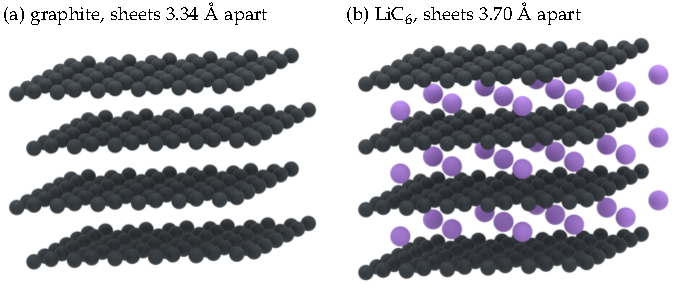
\includegraphics{ch14_pressure/graphite}
\caption{Graphite and LiC$_6$, four sheets of carbon each, seen almost
along the sheets: (a) graphite, stacked A, B, A, B, with the sheets
\SI{3.34}{\angstrom} apart; (b) LiC$_6$, stacked A, A, with lithium
(purple) over every third hexagon between the sheets, \SI{3.70}{\angstrom}
apart (the experimental spacings quoted by Hazrati, de Wijs and
Brocks\cite{Hazrati2014}; the in-plane spacing is kept at graphite's
\SI{2.46}{\angstrom}).}
\label{fig:pr-graphite}
\end{figure}

\subsection*{Three couplings}

For a box whose lattice vectors lie along $x$, $y$ and $z$, a barostat can
respond to the pressure tensor in three ways.
\begin{itemize}
\item \emph{Isotropic}: one factor for all three lengths, from the mean
   of the diagonal, $P$.
\item \emph{Semi-isotropic}: one factor for $x$ and $y$ together, from
   $\frac12(\mathsf{P}_{xx} + \mathsf{P}_{yy})$, and another for $z$, from
   $\mathsf{P}_{zz}$. This suits a layered solid or a
   membrane\cite{Bernetti2020}, whose plane keeps its own symmetry while
   its thickness changes.
\item \emph{Anisotropic}: a factor for each length, from its own diagonal
   component.
\end{itemize}
Changing the angles of the cell as well needs every component of
$\vb{h}$ free, as in Parrinello and Rahman's barostat
(\cref{sec:pr-piston}). \texttt{barostats.Berendsen} takes each of the
three couplings, scaling the length along $\alpha$ by $1 - (\kappa\dt/3
\tau_{\mathrm P})(P_0 - P_\alpha)$ with $P_\alpha$ the pressure that length
responds to; its anisotropic form follows ASE's
\texttt{Inhomogeneous\_NPTBerendsen} to \SI{7.9e-8}{\angstrom} over 40
steps.
Stochastic cell rescaling has a semi-isotropic form too, with its own
drift and noise for the logarithm of the area $A$ normal to $z$ and for
the height $L_z$\cite{Bernetti2020},
\begin{align*}
   \dd\ln A &= -\frac{2\kappa}{3\tau_{\mathrm P}}\Bigl(P_0 -
   \frac{\mathsf{P}_{xx} + \mathsf{P}_{yy}}{2}\Bigr)\dd t + \sqrt{\frac{4\kB T
   \kappa\,\dd t}{3V\tau_{\mathrm P}}}\;g_A ,\\
   \dd\ln L_z &= -\frac{\kappa}{3\tau_{\mathrm P}}\bigl(P_0 - \mathsf{P}_{zz}
   \bigr)\dd t + \sqrt{\frac{2\kB T\kappa\,\dd t}{3V\tau_{\mathrm P}}}\;g_z ,
\end{align*}
with $g_A$ and $g_z$ independent normal numbers. Their sum, since $\ln V =
\ln A + \ln L_z$, is \cref{eq:pr-scr}: the drifts add to
$-(\kappa/\tau_{\mathrm P})(P_0 - P)\,\dd t$, and the variances of the
noises, $\frac23$ and $\frac13$ of $2\kB T\kappa\,\dd t/(V\tau_{\mathrm
P})$, add to the whole of it, since the variances of independent numbers
add (\cref{sec:sm-probability}). The area carries two of the three
lengths and the height one, hence the shares $\frac23$ and $\frac13$.

\subsection*{A layered model solid}

Graphite needs a potential that a later chapter will bring; its point
can be made with Lennard-Jones atoms. The model solid of
\cref{fig:pr-layered} is nine flat sheets of 48 argon-like atoms each, the
atoms of a sheet at the corners of equilateral triangles, stacked so that
each sheet's atoms sit over the hollows of the one below. Atoms within a
sheet attract with eight times argon's depth and 0.95 of its $\sigma$,
atoms in different sheets with argon's own, so the sheets are stiff and
the gaps soft: at 40 K the sheets settle \SI{3.151}{\angstrom} apart, and
the perfect solid, its atoms on their sites in that cell, has $C_{11} =
-\partial\mathsf{P}_{xx}/\partial\epsilon_{xx} = \SI{35.81}{\giga\pascal}$
along the sheets against $C_{33} = -\partial\mathsf{P}_{zz}/\partial
\epsilon_{zz} = \SI{5.31}{\giga\pascal}$ across them, 6.7 times softer.
Between each pair of sheets go twelve guest atoms of lithium's mass, one
for every four sheet atoms, each over a hollow of both sheets, in rows
\SI{7.25}{\angstrom} apart along $x$ and \SI{6.28}{\angstrom} along $y$. They
interact with the sheet atoms through a Lennard-Jones potential of twice
argon's depth, and with each other through one of a fifth of argon's
depth and 1.2 times its $\sigma$. Their reach, the $\sigma$ of their
interaction with the sheets, grows from 1.6 to \SI{2.5}{\angstrom} over
\SI{10}{\pico\second}, pushing the sheets apart through a potential that
changes with time, as the wall pushed in of \cref{sec:en-drift} did, and
is then held for \SI{30}{\pico\second} more, under Berendsen's barostat at
$P_0 = 0$ with each coupling in turn.

\begin{figure}[htb]
\centering
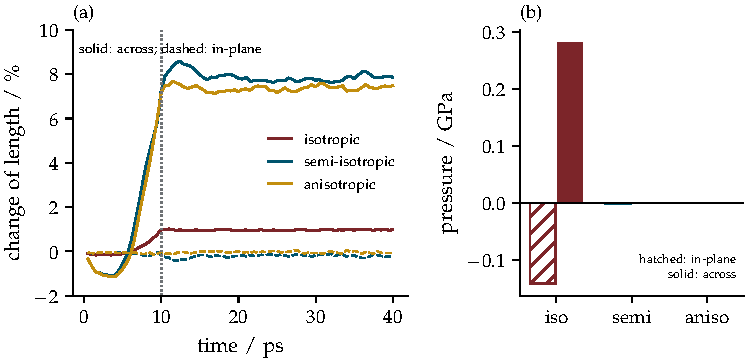
\includegraphics{ch14_pressure/layered}
\caption{Coupling a layered solid. The layered model at \SI{40}{\kelvin}
under Berendsen's barostat at $P_0 = 0$, guests between its sheets whose
reach grows over the first \SI{10}{\pico\second} (dotted) and is then
held for \SI{30}{\pico\second}. (a) The change of the height $c$ of the cell (solid) and of its
in-plane width $a$ (dashed) under isotropic, semi-isotropic and
anisotropic coupling. (b) The pressure in the plane, $\frac12(\mathsf{P}_{xx}
+ \mathsf{P}_{yy})$ (hatched), and across it, $\mathsf{P}_{zz}$ (solid), over the
last \SI{10}{\pico\second}.}
\label{fig:pr-layered}
\end{figure}

Over the last \SI{10}{\pico\second}, under semi-isotropic coupling the
sheets have opened by 7.84\% and the plane has shrunk by 0.20\%, and the
mean pressures in the plane and across it are zero. Under anisotropic
coupling the sheets have opened by 7.42\% and the plane has changed by
less than 0.1\%. Both have settled, the opening wandering by about
0.2\% between successive stretches of \SI{5}{\pico\second}. The two differ
because the rows of guests make the two directions of the plane unequal:
semi-isotropic coupling, which scales $x$ and $y$ together, leaves
$\mathsf{P}_{xx}$ and $\mathsf{P}_{yy}$ at $+0.013$ and
\SI{-0.014}{\giga\pascal}, and anisotropic coupling, which lets each length
move on its own, brings both to zero. Under isotropic coupling every
length grows by 0.97\%: the gaps cannot open as far as the guests need
without the sheets stretching equally, and the solid is left pulled along
its sheets, \SI{-0.141}{\giga\pascal} in the plane, and squeezed across
them, \SI{+0.282}{\giga\pascal}, while the mean of the three, the only
number the isotropic barostat reads, is zero. The early dip of $c$ under
semi-isotropic and anisotropic coupling in \cref{fig:pr-layered}(a), by
about 1\%, comes while the guests' reach is short. Each guest is
\SI{2.60}{\angstrom} from its nearest sheet atoms, which lies beyond the
minimum $2^{1/6}\sigma$ of their pair energy for every $\sigma$ up to
\SI{2.3}{\angstrom}, so until then the guests pull the sheets towards
them.

\begin{keyidea}
A solid that wants to change shape needs a barostat that lets it:
semi-isotropic coupling, one factor for the plane and one across it, for
a layered solid like graphite; anisotropic coupling for each length on its
own, when the directions of the plane differ too. Isotropic coupling of
the layered model with guests between its sheets leaves
\SI{-0.141}{\giga\pascal} along the sheets and \SI{+0.282}{\giga\pascal}
across them while its mean pressure reads zero.
\end{keyidea}

\notebook{14}{insert guests between the sheets under each coupling}

\begin{selfcheck}
A graphite particle opens across its sheets by 10.8\% on lithiation, and
suppose it keeps its in-plane size. By what fraction does its volume grow?
\end{selfcheck}

%=============================================================================!
% 14.9  WHAT THE TRAJECTORY LOOKS LIKE                                        !
%=============================================================================!
\section{What the trajectory looks like}
\label{sec:pr-trajectory}

A run at constant pressure has two more things to read than one at fixed
volume: the volume itself, and a pressure whose single values mean little.
This section shows a healthy run of the liquid and six faults that
pressures and barostats leave, each with the check that catches it.

\subsection*{A healthy run}

\Cref{fig:pr-healthy} follows the liquid for \SI{300}{\pico\second} under
stochastic cell rescaling at \SI{0.1}{\giga\pascal} with $\tau_{\mathrm P}
= \SI{1}{\pico\second}$ and CSVR at \SI{135}{\kelvin}, started from the box
of Chapter~13 at \SI{12577}{\angstrom\cubed}. After the first
\SI{10}{\pico\second} the volume averages \SI{12312}{\angstrom\cubed}, a
density of $0.8172\sigma^{-3}$, and spreads by \SI{190}{\angstrom\cubed},
against the \SI{183}{\angstrom\cubed} of \cref{eq:pr-volume}; it lies within
the predicted \SI{183}{\angstrom\cubed} of its mean for 0.667 of the time,
close to the 0.683 of a Gaussian (\cref{sec:sm-probability}). The instantaneous pressure scatters by \SI{0.0175}{\giga\pascal}
about its mean of \SI{0.0988}{\giga\pascal}: for 256 atoms a single value of
$P$ says little, and only its average is compared with the target. The
sum $K + U + P_0V$ wanders over \SI{9.50}{\milli\electronvolt} per atom as
the thermostat and the barostat exchange energy with the liquid, while the
effective energy, that sum less the heat and the work, stays within
\SI{0.027}{\milli\electronvolt} per atom and drifts by
\SI{-6.4e-6}{\electronvolt\per\pico\second} for the whole liquid. The kinetic temperature
averages \SI{134.69}{\kelvin}.

\begin{figure}[htb]
\centering
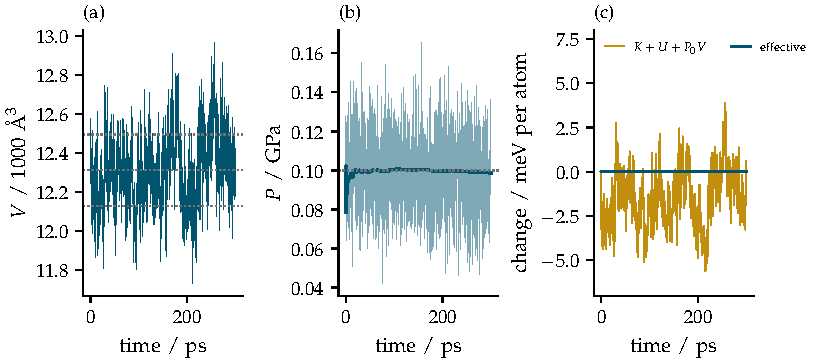
\includegraphics{ch14_pressure/healthy}
\caption{A healthy run at constant pressure: the liquid under stochastic
cell rescaling at \SI{0.1}{\giga\pascal} and CSVR at \SI{135}{\kelvin}, for
\SI{300}{\pico\second}. (a) The volume every \SI{100}{\femto\second}, with
its mean and the spread $\sqrt{\kB T\ens{V}\kappa_T}$ either side (dotted).
(b) The instantaneous pressure (thin) and its running mean (thick),
against the target (dotted). (c) $K + U + P_0V$ per atom and the effective
energy, that less the heat and the barostat's work, from their starting
values.}
\label{fig:pr-healthy}
\end{figure}

\subsection*{Six faults}

\Cref{fig:pr-faults} shows six faults and \cref{tab:pr-faults} the check
that catches each.

\begin{figure}[p]
\centering
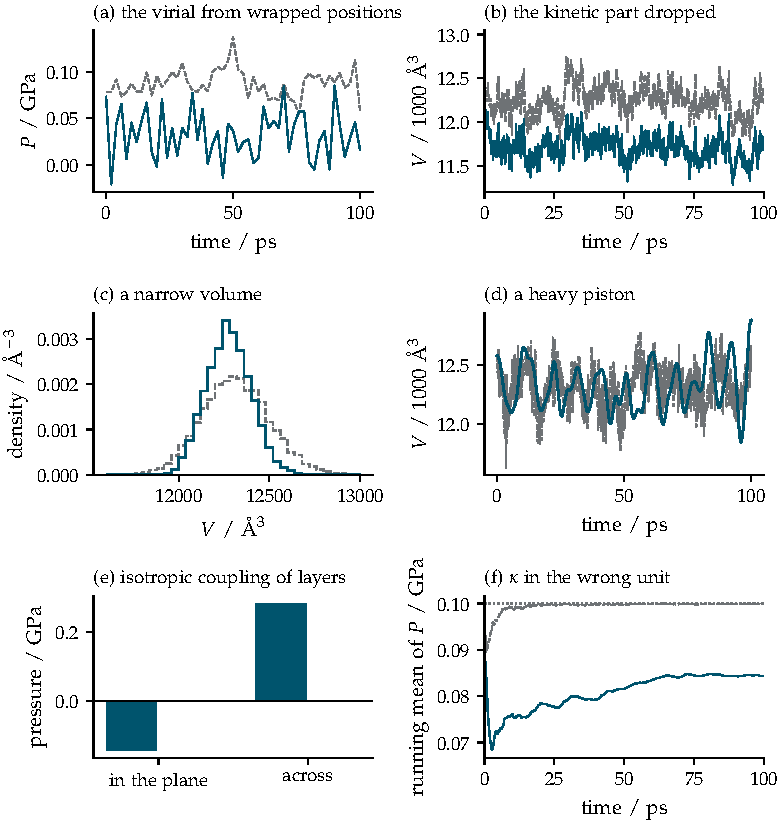
\includegraphics{ch14_pressure/faults}
\caption{Pressure and barostat faults (teal) against healthy runs (grey
dashed). (a) The pressure of the liquid at fixed volume from
$\sum_i\vb{r}_i\cdot\vb{F}_i$ with wrapped positions, against the pair
form. (b) The volume under cell rescaling given the virial's pressure
without the kinetic part. (c) The density of the volume under
Berendsen's barostat, against cell rescaling. (d) The volume under a
piston with $\tau_{\mathrm P} = \SI{10}{\pico\second}$, against
\SI{1}{\pico\second}. (e) The layered solid with guests: the pressure in
its plane and across it under isotropic coupling, against
semi-isotropic coupling (grey, zero). (f) The running mean of the
pressure under Berendsen's barostat given $\kappa$ in bar$^{-1}$ where
GPa$^{-1}$ was meant, against the right $\kappa$, with the target
(dotted).}
\label{fig:pr-faults}
\end{figure}

\begin{table}[htb]
\centering
\caption{The faults of \cref{fig:pr-faults}, the check that catches each,
and its value in the healthy and the broken run.}
\label{tab:pr-faults}
\small
\begin{tabular}{@{}>{\raggedright\arraybackslash}p{0.27\linewidth}
   >{\raggedright\arraybackslash}p{0.33\linewidth}ll@{}}
\toprule
fault & check & healthy & broken\\
\midrule
(a) virial from wrapped positions & $P$ before and after moving the
   origin, GPa &
   0.0877, 0.0877 & 0.0324, 0.0354\\
(b) kinetic part dropped & $\ens{P}$ with $2K$ included, GPa & 0.0988 &
   0.1411\\
(c) volume too narrow & $\kappa_T$ from the fluctuations, GPa$^{-1}$ &
   1.50 & 0.64\\
(d) piston too heavy & swings of $V$ in \SI{90}{\pico\second} & 103 & 10\\
(e) isotropic coupling of layers & $\frac12(\mathsf{P}_{xx} +
   \mathsf{P}_{yy})$, $\mathsf{P}_{zz}$, GPa & 0.000, 0.000 & $-0.141$,
   0.282\\
(f) $\kappa$ in the wrong unit & $\ens{P}$ after the first
   \SI{50}{\pico\second}, GPa & 0.1001 & 0.0871\\
\bottomrule
\end{tabular}
\end{table}

\emph{(a) The virial from wrapped positions.} As \cref{sec:pr-periodic}
showed, $\sum_i\vb{r}_i\cdot\vb{F}_i$ with wrapped positions gives
\SI{0.0324}{\giga\pascal} for a liquid whose pressure is
\SI{0.0877}{\giga\pascal}, and a different value when the origin moves.
The check is to move the origin: a correct pressure does not change.

\emph{(b) The kinetic part dropped.} A barostat handed only $\mathcal{W}/3V$,
as happens when ASE's \texttt{get\_stress} is called without
\texttt{include\_ideal\_gas=True}, holds that part at $P_0$ and lets the
true pressure rise by $N\kB T/V$, here \SI{0.0408}{\giga\pascal}: the
liquid shrinks by 4.9\%, to \SI{11706}{\angstrom\cubed} from
\SI{12312}{\angstrom\cubed}, and its full pressure reads
\SI{0.1411}{\giga\pascal}. The check is the mean of $(2K +
\mathcal{W})/3V$ against $P_0$.

\emph{(c) A volume too narrow.} Berendsen's barostat holds the mean
pressure, so nothing in one run looks wrong; the check is $\kappa_T$ from
the volume's fluctuations, \cref{eq:pr-volume}, against an independent
value: \SI{0.64}{\per\giga\pascal} under Berendsen's barostat,
\SI{1.50}{\per\giga\pascal} under cell rescaling, and
\SI{1.46}{\per\giga\pascal} from the runs at fixed volume.

\emph{(d) A piston too heavy.} With $\tau_{\mathrm P} =
\SI{10}{\pico\second}$ the volume swings with a period of
\SI{8.7}{\pico\second}, 10 times in \SI{90}{\pico\second}, so the run's
mean volume rests on ten swings; with \SI{1}{\pico\second} it swings 103
times. The check is the period of the volume against the length of the
run.

\emph{(e) Isotropic coupling of a layered solid.} The mean pressure reads
the target while the solid is pulled along its sheets and squeezed across
them, $-0.141$ and \SI{+0.282}{\giga\pascal}. The check is the diagonal
of the pressure tensor, component by component.

\emph{(f) The compressibility in the wrong unit.} The barostat's $\kappa$
for the liquid, \SI{2.5}{\per\giga\pascal}, is $2.5\times10^{-4}$ per bar; entered
as $2.5\times10^{-4}$ where gigapascals were meant, it makes Berendsen's
barostat $10^4$ times slower, a relaxation time of
\SI{5.8}{\nano\second} instead of \SI{0.58}{\pico\second}. The volume
stays where it started, \SI{12577}{\angstrom\cubed}, and the pressure
stays at \SI{0.0871}{\giga\pascal} against the target 0.1. The check is
the running mean of the pressure against the target, and the volume's
relaxation against $\tau_{\mathrm P}$.

\begin{practice}
A run at constant pressure is read through the running mean of its
pressure, computed with the kinetic part and from pair separations, which
should settle at $P_0$; through the spread of its volume, which should be
$\sqrt{\kB T\ens{V}\kappa_T}$, with $\kappa_T$ checked at fixed volumes;
through the diagonal of its pressure tensor, which for a solid should
match $P_0$ in every component the coupling lets relax; and through the
period of its volume, or its relaxation time when the barostat has no
piston, against the length of the run. Berendsen's barostat serves to
bring a system to its pressure; stochastic cell rescaling or a piston
with chains then samples it, and $\tau_{\mathrm P} = \SI{1}{\pico\second}$
sampled the liquid's volume correctly here, with 103 swings of the piston
in \SI{90}{\pico\second}; a layered solid needs semi-isotropic coupling, or
anisotropic coupling when the directions of its plane differ.
\end{practice}

\begin{keyidea}
In a healthy run at constant pressure the instantaneous pressure
scatters widely, its running mean settles at the target, the volume
spreads by $\sqrt{\kB T\ens{V}\kappa_T}$, and the effective energy holds
still. A virial from wrapped positions, a pressure without its kinetic
part, Berendsen's narrow volume, a piston too heavy, isotropic coupling of
a solid that wants to change shape, and a compressibility in the wrong
unit each leave a mark that a single check catches.
\end{keyidea}

\notebook{14}{break the run at constant pressure in each of the six ways and read the checks}

\begin{selfcheck}
For a liquid of 500 atoms at \SI{300}{\kelvin} in
\SI{20000}{\angstrom\cubed}, minus the mean of the diagonal of ASE's
\texttt{get\_stress()}, called with its defaults, averages
\SI{-0.04}{\giga\pascal}. What is the liquid's pressure?
\end{selfcheck}

%=============================================================================!
% 14.S  WHAT WE NOW HAVE                                                      !
%=============================================================================!
\unnumbered{What we now have}

The pressure of a gas is the momentum its atoms deliver to the walls per
unit time and area, $N\kB T/V$ for atoms that do not interact.
Equipartition applied to the positions adds the virial's share, $PV =
N\kB T + \frac13\ens{\mathcal{W}}$, and the free energy's response to a
change of volume gives the same formula in a periodic box, with the virial
summed over pairs from their separations to the nearest copy; the sum
$\sum_i\vb{r}_i\cdot\vb{F}_i$ from wrapped positions changes with the
origin.

Its response to a strain gives the pressure tensor,
$(\sum_im_iv_{i\alpha}v_{i\beta} + \mathcal{W}_{\alpha\beta})/V$, isotropic for
a liquid, uneven for a strained solid; ASE and many libraries report the
stress, its negative.

A barostat must sample $\mathcal{P}(V) \propto
\mathrm{e}^{-\beta P_0V}Z(N, V, T)$, which for an ideal gas is
$V^N\mathrm{e}^{-\beta P_0V}$ and for a liquid has the variance $\kB
T\ens{V}\kappa_T$.

Berendsen's barostat holds the mean pressure but squeezes the
volume's fluctuations, which then give less than half the liquid's
compressibility; stochastic cell
rescaling adds to $\ln V$ the noise the fluctuation-dissipation relation
demands and samples the volume correctly; the MTK piston gives the volume
a mass, swings with the period $2\pi\tau_{\mathrm P}\sqrt{(N + 1)\kB T
\kappa_T/3V}$, and with chains samples correctly too.

A solid that wants to
change shape needs semi-isotropic or anisotropic coupling: isotropic
coupling of a layered solid with guests between its sheets leaves it
pulled along the sheets and squeezed across them while its mean pressure
reads the target.

A healthy run shows a widely scattered instantaneous
pressure whose running mean settles at $P_0$, a volume that spreads by
$\sqrt{\kB T\ens{V}\kappa_T}$, and an effective energy that holds still.

Chapter~15 asks how long a run must be before such averages, and the
error bars on them, can be trusted.

%=============================================================================!
% 14.A  ANSWERS TO THE CHECKS                                                 !
%=============================================================================!
\unnumbered{Answers to the checks}
\label{sec:pr-answers}

\answerto{sec:pr-wall}$P = N\kB T/V = 10^4\times0.025852/100^3 =
\SI{2.585e-4}{\electronvolt\per\angstrom\cubed}$, which is $2.585\times
10^{-4}\times160.218\times10^4 = \SI{414.2}{bar}$.

\answerto{sec:pr-virial}They raise it. Closer than the minimum,
$\varphi'(r) < 0$: the atoms repel, and the pair adds $-r\varphi'(r) > 0$ to
$\mathcal{W}$, and so raises $(2K + \mathcal{W})/3V$ above the $2K/3V$ of
two atoms that do not interact.

\answerto{sec:pr-periodic}$V$ is proportional to $a^3$, and the factor
cancels in $V/\Delta V$, so $B \approx -V_{\mathrm m}\,\Delta P/\Delta V$
with $V_{\mathrm m}$ the mean of $5.20^3$ and $5.40^3$: $B \approx 149.04
\times0.288/16.86 = \SI{2.55}{\giga\pascal}$. The two spacings are centred
on \SI{5.30}{\angstrom}, on the stretched side of $a_0$, where the crystal
is softer, so the estimate lies below the \SI{2.856}{\giga\pascal} at
$a_0$.

\answerto{sec:pr-tensor}$P = -0.002\times160.218 =
\SI{-0.320}{\giga\pascal}$: the stress is positive, so the material pulls
on its cell.

\answerto{sec:pr-npt}$1/\sqrt{1001} = 0.0316$, about 3\%.

\answerto{sec:pr-rescaling}$1 - (2.5\times0.01/3)(0.1 - 0.08) =
0.9998333$: each length shrinks by 17 parts in a hundred thousand, which
raises the pressure towards its target.

\answerto{sec:pr-piston}$\omega^2 = A^2/(M_{\mathrm p}V\kappa) =
(10^{-3})^2/(1\times10^{-3}\times10^{-5}) = \SI{100}{\per\second\squared}$,
so $\omega = \SI{10}{\radian\per\second}$ and the period is
\SI{0.628}{\second}.

\answerto{sec:pr-shape}The volume is the in-plane area times the height,
and with the area kept it grows as the height does: by 10.8\%.

\answerto{sec:pr-trajectory}\texttt{get\_stress} leaves out the kinetic
part by default; adding $N\kB T/V = 500\times0.025852/20000 =
\SI{6.46e-4}{\electronvolt\per\angstrom\cubed} = \SI{0.1035}{\giga\pascal}$
gives $-0.04 + 0.1035 = \SI{0.0635}{\giga\pascal}$.

%=============================================================================!
% 14.E  EXERCISES                                                             !
%=============================================================================!
\unnumbered{Exercises}
\label{sec:pr-exercises}

The exercises run from questions of understanding, through calculations,
to short derivations marked `show that'. Full solutions are in
\hyperref[sec:pr-solutions]{`Solutions to the exercises'} at the end of
the book, and Notebook~14 checks every numerical answer.

\begin{exercise}[units of pressure]
\label{ex:pr-units}
Show that \SI{1}{\electronvolt\per\angstrom\cubed} is
\SI{160.218}{\giga\pascal}, and express one bar in
\si{\electronvolt\per\angstrom\cubed}.
\end{exercise}

\begin{exercise}[air]
\label{ex:pr-air}
Find the number of molecules per \si{\angstrom\cubed} in air at one bar and
\SI{300}{\kelvin}, treated as an ideal gas, and the spacing $(V/N)^{1/3}$
between molecules.
\end{exercise}

\begin{exercise}[atoms in every direction]
\label{ex:pr-flux}
Atoms of mass $m$ at the number density $\rho$ move in every direction, a
fraction $\mathcal{P}(v_x)\,\dd v_x$ of them with velocity along $x$
between $v_x$ and $v_x + \dd v_x$ (\cref{sec:sm-maxwell}). Show, by
counting the atoms with $v_x > 0$ that reach a wall of area $A$ in a time
$t$, each delivering $2mv_x$, that the pressure is $\rho m\ens{v_x^2}$, the
average taken over all the atoms, and hence $\rho\kB T$.
\end{exercise}

\begin{exercise}[the sign of a pair's share]
\label{ex:pr-sign}
For the Lennard-Jones potential of argon, with $\sigma =
\SI{3.4}{\angstrom}$, find the distance at which a pair's contribution
$-r\varphi'(r)$ to the virial changes sign, and the sign of that
contribution closer in.
\end{exercise}

\begin{exercise}[the origin at the centre]
\label{ex:pr-centre}
Show that the walls' share, $\sum_i\vb{r}_i\cdot\vb{F}^{\mathrm w}_i$, is
still $-3PV$ when the origin is placed at the centre of the box, with the
walls at $x = \pm L/2$.
\end{exercise}

\begin{exercise}[wrapping one atom]
\label{ex:pr-wrap}
Show that wrapping a single atom $i$ back into a cubic cell of side $L$
along $x$ changes $\sum_j\vb{r}_j\cdot\vb{F}_j$ by $\pm LF_{ix}$, while
leaving \cref{eq:pe-virial}, written with nearest-copy separations,
unchanged.
\end{exercise}

\begin{exercise}[a determinant to first order]
\label{ex:pr-det}
Show, by writing out the triple product $\vb{c}_1\cdot(\vb{c}_2\times
\vb{c}_3)$ of the columns of $\vb{I} + \boldsymbol{\epsilon}$
(\cref{sec:ro-tensor}), that $\det(\vb{I} + \boldsymbol{\epsilon}) = 1 +
\epsilon_{xx} + \epsilon_{yy} + \epsilon_{zz}$ plus terms of second and
third order in the components of $\boldsymbol{\epsilon}$.
\end{exercise}

\begin{exercise}[the trace of the tensor]
\label{ex:pr-trace}
Show that one third of the trace of \cref{eq:pr-tensor} is the
instantaneous pressure $(2K + \mathcal{W})/3V$ of \cref{sec:pr-virial}.
\end{exercise}

\begin{exercise}[a cubic crystal's bulk modulus]
\label{ex:pr-cubic}
For a cubic crystal, each diagonal component $\mathsf{P}_{\alpha\alpha}$ of
the pressure tensor falls by $C_{11}$ for each unit of its own strain
$\epsilon_{\alpha\alpha}$ and by $C_{12}$ for each unit of the strain along
either other axis. Show that $B = (C_{11} + 2C_{12})/3$, and evaluate it
for the crystal of \cref{sec:pr-tensor}.
\end{exercise}

\begin{exercise}[integrals of the gamma kind]
\label{ex:pr-gamma}
Show that $\int_0^\infty V^n\mathrm{e}^{-bV}\dd V = n!/b^{n+1}$ for $b > 0$
and every whole number $n$, by integrating by parts and using the result
for $n - 1$.
\end{exercise}

\begin{exercise}[a small ideal gas]
\label{ex:pr-ideal}
For 20 atoms that do not interact, at \SI{135}{\kelvin} and $P_0 =
\SI{1e-4}{\electronvolt\per\angstrom\cubed}$, find the mean volume and its
spread, and compare the mean with $N\kB T/P_0$.
\end{exercise}

\begin{exercise}[where Berendsen's barostat leaves an ideal gas]
\label{ex:pr-berendsen-mean}
Berendsen's barostat drives the instantaneous pressure, $2K/3V$ for an
ideal gas, to $P_0$ on average. Assuming the volume's spread small and $K$
independent of $V$, show that the mean volume settles near $N\kB T/P_0$ for
a run whose $\ens{2K} = 3N\kB T$.
\end{exercise}

\begin{exercise}[how fast the volume settles]
\label{ex:pr-relax}
For the liquid, with $\kappa_T = \SI{1.46}{\per\giga\pascal}$ and
$\tau_{\mathrm P} = \SI{1}{\pico\second}$, find the time in which the volume
relaxes under Berendsen's barostat given $\kappa = \SI{2.5}{\per\giga
\pascal}$, and given $\kappa = 2.5\times10^{-4}$\,\si{\per\giga\pascal}.
\end{exercise}

\begin{exercise}[the spread of the logarithm]
\label{ex:pr-logspread}
Find the spread of $\ln V$ that stochastic cell rescaling should give the
liquid at \SI{135}{\kelvin}, with $\kappa_T = \SI{1.46}{\per\giga\pascal}$
and $V = \SI{12306}{\angstrom\cubed}$.
\end{exercise}

\begin{exercise}[the kinetic energy of a growing box]
\label{ex:pr-kinetic}
With each momentum written as $\vb{p}_i = \boldsymbol{\pi}_i V^{-1/3}$,
show that $\partial K/\partial V$ at fixed $\boldsymbol{\pi}_i$ is
$-2K/3V$.
\end{exercise}

\begin{exercise}[a gas at fixed temperature]
\label{ex:pr-gas-kappa}
Show that an ideal gas held at a fixed temperature has $\kappa_T = 1/P$.
\end{exercise}

\begin{exercise}[Andersen's piston]
\label{ex:pr-andersen}
A barostat whose coordinate is the volume itself, with the mass
$M_V$, obeys $M_V\ddot V = P - P_0$. Show that it swings with $\omega^2 =
1/(M_VV\kappa_T)$ about its mean.
\end{exercise}

\begin{exercise}[the piston's period]
\label{ex:pr-period}
From $\omega^2 = 9V/(M_\epsilon\kappa_T)$ and $M_\epsilon = (3N + 3)\kB T
\tau_{\mathrm P}^2$, show that the period is $2\pi\tau_{\mathrm P}
\sqrt{(N + 1)\kB T\kappa_T/3V}$, and evaluate the factor for the liquid
of 256 atoms at \SI{135}{\kelvin}, with $V = \SI{12306}{\angstrom\cubed}$
and $\kappa_T = \SI{1.46}{\per\giga\pascal}$.
\end{exercise}

\begin{exercise}[graphite, isotropically]
\label{ex:pr-graphite}
If the 10.8\% growth of volume in the check of \cref{sec:pr-shape}, in
which the in-plane size is kept, were shared equally by the three lengths,
by how much would each grow?
\end{exercise}

\begin{exercise}[the kinetic part dropped]
\label{ex:pr-dropped}
A barostat that sees only $\mathcal{W}/3V$ holds the liquid at the true
pressure $P_0 + N\kB T/V$. Estimate from $\kappa_T$ by what fraction its
volume shrinks, and compare with the 4.9\% of \cref{sec:pr-trajectory}.
Why is the estimate larger?
\end{exercise}

\begin{exercise}[a referee's objection]
\label{ex:pr-referee}
A study reports the compressibility of a liquid from the fluctuations of
its volume, \cref{eq:pr-volume}, in a run under Berendsen's barostat. What
is wrong, which way is the result wrong, and which barostat would fix
it?
\end{exercise}


%=============================================================================!
% CHAPTER 15  EQUILIBRATION, CONVERGENCE AND UNCERTAINTY                      !
%=============================================================================!
\chapter{Equilibration, convergence and uncertainty}
\label{ch:convergence}

%=============================================================================!
% 15.0  CHAPTER OPENING                                                       !
%=============================================================================!
Many results of a simulation are averages over a run of finite length.
A second run from another start would give a slightly different value.
Chapters~11 to~14 quoted such averages, sometimes with the spread of a
few runs, but left open how accurately they were known. An error bar
makes that question explicit when we compare a result with experiment,
another code or another thermostat. It does not remove a bias: an early
interval in which the system is still settling shifts the average, and
extending the run only dilutes that shift.

We first find the error of a mean from independent samples, then account
for the memory between successive samples of a trajectory. Block averages
provide a second estimate and a visible check on whether the record is
long enough. These tools let us choose where to begin averaging, test for
drift and estimate the time needed for a chosen precision.

Convergence in time is only part of the problem. We also test the size of
the periodic box and whether the thermostat samples its stated ensemble.
The chapter ends with a protocol for preparing a run and a numerical
criterion for each reported quantity. Chapter~16 uses these checks to
measure structure and motion.

%=============================================================================!
% 15.1  THE ERROR OF AN AVERAGE                                               !
%=============================================================================!
\section{The error of an average}
\label{sec:cv-mean}

A run reports the average of a quantity over its samples, and that average
misses the ensemble average by an amount that changes from run to run.
This section finds the size of the miss when the samples are independent,
on rolls of a die first, and says what an error bar built from it
promises.

\subsection*{The mean of independent rolls}

A fair die shows each face with probability $\frac16$, so one roll $x$ has
the mean $\ens{x} = 3.5$ and the variance $\sigma_x^2 = 35/12$
(\cref{ex:sm-die}). Rolling it $n$ times and averaging gives
\begin{equation*}
   \bar x = \frac1n\sum_{i=1}^nx_i ,
\end{equation*}
the overbar marking an average over samples, as it marks an average over
time (\cref{sec:sm-ergodic}). Each roll has the mean $\ens{x}$, and the
expectation of a sum is the sum of the expectations, so $\ens{\bar x} =
n\ens{x}/n = \ens{x}$: many such averages centre on the right value.
Their spread follows from the rule of \cref{sec:sm-probability} that the
variances of independent quantities add, and from one more. The rolls are
independent, so the variances of the $n$ of them add,
$\operatorname{var}(\sum_ix_i) = n\sigma_x^2$. A constant factor $a$
multiplies a variance by $a^2$, since
\begin{equation*}
   \operatorname{var}(ax) = \ens{a^2x^2} - \ens{ax}^2
   = a^2\bigl(\ens{x^2} - \ens{x}^2\bigr) = a^2\operatorname{var}(x) ,
\end{equation*}
and with $a = 1/n$,
\begin{equation}
   \operatorname{var}(\bar x) = \frac{n\sigma_x^2}{n^2}
   = \frac{\sigma_x^2}{n} , \qquad
   \sigma_{\bar x} = \frac{\sigma_x}{\sqrt n} .
   \label{eq:cv-mean}
\end{equation}
The spread of the mean falls as the square root of the number of samples:
four times as many rolls halve it, and a hundred times as many cut it to a
tenth. \Cref{fig:cv-dice}(b) rolls the die by computer, $n$ rolls at a
time, 200\,000 times over: the spread of the mean is 0.8558 for 4 rolls
against $\sigma_x/\sqrt4 = 0.8539$, and 0.1067 for 256 rolls against
0.1067.

\Cref{fig:cv-dice}(a) shows the shape as well as the spread. One roll has
six equally likely values, but the mean of 4 rolls is already close to
the Gaussian of \cref{eq:sm-gauss} with mean 3.5 and variance $\sigma_x^2/4$,
and the mean of 64 is indistinguishable from its Gaussian. The mean of
many independent samples approaches a Gaussian density whatever the
density of one sample, provided that density has a finite variance, a
result known as the central limit theorem, which the figure illustrates
without proving\cite{Grossfield2018}.

\begin{figure}[htb]
\centering
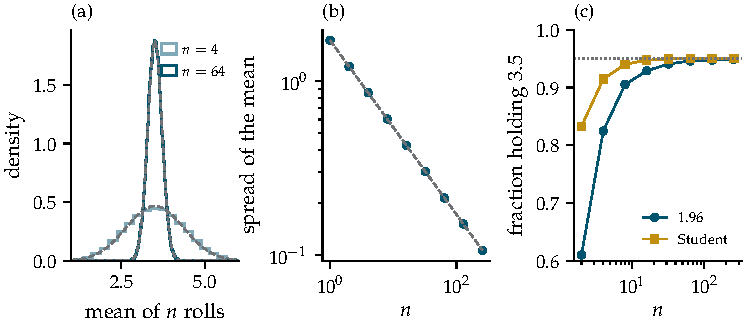
\includegraphics{ch15_convergence/dice}
\caption{The error of an average of independent rolls of a die, each set
of $n$ rolls repeated 200\,000 times. (a) The density of the mean of 4
rolls (light) and of 64 (dark), against the Gaussians of mean 3.5 and
variance $\sigma_x^2/n$ (dashed). (b) The spread of the mean against $n$,
against $\sigma_x/\sqrt n$ (dashed). (c) The fraction of the intervals
$\bar x \pm 1.96\,s/\sqrt n$ that hold 3.5 (teal), and of those with
Student's factor in place of 1.96 (ochre), against 0.95 (dotted).}
\label{fig:cv-dice}
\end{figure}

\subsection*{The standard error}

In a simulation $\sigma_x$ is not known in advance and must be estimated
from the same samples. The spread of the samples about their own mean
falls short of $\sigma_x$, because $\bar x$ sits closer to the samples than
$\ens{x}$ does. Writing each deviation as $x_i - \bar x = (x_i - \ens{x})
- (\bar x - \ens{x})$ and expanding the square,
\begin{align*}
   \sum_i(x_i - \bar x)^2
   &= \sum_i(x_i - \ens{x})^2 - 2(\bar x - \ens{x})\sum_i(x_i - \ens{x})
   + n(\bar x - \ens{x})^2\\
   &= \sum_i(x_i - \ens{x})^2 - n(\bar x - \ens{x})^2 ,
\end{align*}
since $\sum_i(x_i - \ens{x}) = n(\bar x - \ens{x})$. Averaging, the first sum gives
$n\sigma_x^2$ and the second term $n\operatorname{var}(\bar x) =
\sigma_x^2$, so the sum of squares averages to $(n - 1)\sigma_x^2$.
Dividing by $n - 1$ rather than $n$ therefore gives an estimate whose
average is $\sigma_x^2$,
\begin{equation*}
   s^2 = \frac{1}{n - 1}\sum_i(x_i - \bar x)^2 ,
\end{equation*}
and the estimate of $\sigma_{\bar x}$ is $s/\sqrt n$, the standard error of
the mean. The book writes a result as $\bar x \pm s/\sqrt n$, one standard
error, unless a factor is stated.

\subsection*{What an error bar promises}

When the mean is Gaussian, it lies within one $\sigma_{\bar x}$ of
$\ens{x}$ in 68.27\% of runs and within two in 95.45\%
(\cref{sec:sm-probability}); the factor that encloses 95\%, found
numerically from $\operatorname{erf}(1.960/\sqrt2) = 0.95$, is 1.960. An interval $\bar x \pm
1.96\,s/\sqrt n$ should therefore hold the true mean in 95\% of runs, and
\cref{fig:cv-dice}(c) counts how often it does: 0.949 of the time for 256
rolls and 0.905 for 8; for 3 rolls, not drawn, it is 0.777. With few
samples the estimate $s$ is itself uncertain, and a run whose $s$ happens
to be small claims an interval too narrow. For samples with a Gaussian
density the remedy is exact: Student showed that $(\bar x - \ens{x})/(s/
\sqrt n)$ then has a known density that depends on $n$ only through $n -
1$, its number of degrees of freedom. The $n$ deviations $x_i - \bar x$
from which $s$ is built add to zero, which leaves $n - 1$ of them free, as
holding the total momentum at zero left $3N - 3$ velocities free
(\cref{sec:sm-equipartition}). The density's 95\% factor is 4.303 for
three samples, 2.365 for 8 and 1.998 for 64, and approaches 1.960 as $n$
grows\cite{Student1908}. Three Gaussian samples with the factor 1.96
hold their mean in 0.811 of trials, as Student's density predicts; with
4.303 in 0.950. The die is far from Gaussian, and Student's factor brings
its three rolls only to 0.917. The standard errors of three runs that
Chapter~13 quoted are of this kind. For the difference of two means of
three runs each, Student's density has, when the two spreads are alike,
$2 + 2 = 4$ degrees of freedom and the 95\% factor 2.776, so the
differences of up to 2.5 combined errors that \cref{sec:th-compare} found
for the Nosé-Hoover chains and CSVR are within what so few runs leave open,
and the 2.9 of Berendsen coupling lies only just beyond it.
\Cref{sec:cv-observables} returns to those numbers with error bars from
the runs themselves.

\begin{keyidea}
The mean of $n$ independent samples has the spread $\sigma_x/\sqrt n$, and
approaches a Gaussian as $n$ grows whatever the samples' own density,
provided its variance is finite. Its
standard error is $s/\sqrt n$, with $s^2$ the sum of squared deviations
divided by $n - 1$. The interval $\pm1.96$ standard errors holds the true
mean in 95\% of runs when $n$ is large; with few samples it holds it less
often, and Student's factor replaces 1.96.
\end{keyidea}

\notebook{15}{roll dice and watch the mean narrow and the error bars cover}

\begin{selfcheck}
A run of 100 independent samples gives a standard error of 0.05. How many
samples give 0.01?
\end{selfcheck}

%=============================================================================!
% 15.2  SAMPLES THAT REMEMBER                                                 !
%=============================================================================!
\section{Samples that remember}
\label{sec:cv-correlation}

The samples of a run are not independent. In one step of
\SI{10}{\femto\second} an atom moves a small fraction of its distance to a
neighbour, so the potential energy, the kinetic energy and the pressure
change little from one step to the next, and a sample says much about the
one after it. This section measures that memory, finds how it enlarges the
error of a mean, and estimates it from a single run.

\subsection*{A series with memory}

A grain of dust in still air is pushed about by the molecules that strike
it, and its velocity changes over a time set by the friction of the air.
\Cref{sec:th-langevin} found the exact law of one component of such a
velocity over a step: the Ornstein-Uhlenbeck process of \cref{eq:th-ou}.
Measured in units of its own standard deviation, so that its variance is
1, it reads
\begin{equation}
   x_{k+1} = c\,x_k + \sqrt{1 - c^2}\;z_k , \qquad 0 \le c < 1 ,
   \label{eq:cv-ou}
\end{equation}
with $z_k$ a fresh Gaussian number of mean 0 and variance 1 at each step
(the $g$ of \cref{eq:th-ou}, renamed because $g$ is needed below).
The old value keeps the fraction $c$ of itself, and the noise supplies the
variance that this loses, $1 - c^2$. With $c = 0$ each sample is new; with
$c$ close to 1 the series wanders slowly. \Cref{fig:cv-ou}(a) draws 400
samples with $c = 0.95$, read as samples \SI{10}{\femto\second} apart,
against 400 independent ones: the first stays on one side of zero for up
to \SI{0.98}{\pico\second} at a time, while the second changes sign on
average every other sample.

\subsection*{The autocorrelation function}

The memory is measured by the covariance of two quantities,
\begin{equation*}
   \operatorname{cov}(x, y) = \ens{(x - \ens{x})(y - \ens{y})}
   = \ens{xy} - \ens{x}\ens{y} ,
\end{equation*}
the bracket of \cref{sec:sm-probability} that vanished for independent
quantities, which by the same expansion makes $\operatorname{var}(x + y) =
\operatorname{var}(x) + \operatorname{var}(y) + 2\operatorname{cov}(x, y)$.
A run that has settled has the same statistics wherever in it they are
measured, so the covariance of the samples $A_i$ and $A_{i+k}$ depends on
their separation $k$ alone. Divided by the variance, it is the
autocorrelation function
\begin{equation*}
   \operatorname{corr}(k) = \frac{\operatorname{cov}(A_i,
   A_{i+k})}{\operatorname{var}(A)} ,
\end{equation*}
equal to 1 at $k = 0$ and falling towards 0 as the series forgets. For the
series of \cref{eq:cv-ou}, multiplying both sides by $x_0$ and averaging
gives
\begin{equation*}
   \ens{x_{k+1}x_0} = c\ens{x_kx_0} + \sqrt{1 - c^2}\,\ens{z_kx_0}
   = c\ens{x_kx_0} ,
\end{equation*}
since $z_k$ is drawn after $x_0$ and independently of it, with mean zero.
Applying this $k$ times from $\ens{x_0x_0} = 1$ gives $\ens{x_kx_0} = c^k$,
and with the means zero and the variance 1 this is $\operatorname{corr}(k)
= c^k$, which falls by the factor $c$ each step. Here $\dt$ is the time
between samples, one integration step in this chapter's runs, and $c^k =
\mathrm{e}^{-k\dt/\tau_{\mathrm c}}$ with the correlation time $\tau_{\mathrm
c} = -\dt/\ln c$, which is $1/\gamma$ for Langevin's $c =
\mathrm{e}^{-\gamma\dt}$. For $c = 0.95$ and $\dt = \SI{10}{\femto
\second}$, $\tau_{\mathrm c} = \SI{195.0}{\femto\second}$.

\subsection*{The variance of a correlated mean}

The mean $\bar A$ of $n$ samples has the variance of their sum divided by
$n^2$. The square of a sum of deviations $\delta A_i = A_i - \ens{A}$ is
the sum of all their products, $(\sum_i\delta A_i)^2 =
\sum_i\sum_j\delta A_i\,\delta A_j$, so
\begin{equation*}
   \operatorname{var}(\bar A) = \frac{1}{n^2}\sum_{i=1}^n\sum_{j=1}^n
   \operatorname{cov}(A_i, A_j)
   = \frac{\sigma_A^2}{n^2}\sum_{i=1}^n\sum_{j=1}^n
   \operatorname{corr}(\lvert i - j\rvert) ,
\end{equation*}
the second form using the autocorrelation function at the lag $\lvert i -
j\rvert$, since $\operatorname{cov}(A_i, A_j) = \operatorname{cov}(A_j,
A_i)$. The pairs with $i = j$ number $n$, each contributing 1; those $k$ apart,
with $k$ from 1 to $n - 1$, number $n - k$ with $j$ after $i$ and as many
with $j$ before. Collecting them,
\begin{equation}
   \operatorname{var}(\bar A)
   = \frac{\sigma_A^2}{n^2}\Bigl[n + 2\sum_{k=1}^{n-1}(n - k)
   \operatorname{corr}(k)\Bigr]
   = \frac{\sigma_A^2}{n}\Bigl[1 + 2\sum_{k=1}^{n-1}\Bigl(1 - \frac kn\Bigr)
   \operatorname{corr}(k)\Bigr] .
   \label{eq:cv-var}
\end{equation}
For independent samples the bracket is 1 and this is \cref{eq:cv-mean}. A
run is normally far longer than its memory, so $k/n$ is negligible
wherever $\operatorname{corr}(k)$ is not, and the bracket settles to the
statistical inefficiency\cite{Chodera2007}
\begin{equation*}
   g = 1 + 2\sum_{k=1}^{\infty}\operatorname{corr}(k) , \qquad
   \operatorname{var}(\bar A) = \frac{g\,\sigma_A^2}{n} .
\end{equation*}
Correlated samples spread the mean $\sqrt g$ times as widely as the same
number of independent ones: $n$ of them are worth $n_{\mathrm{eff}} = n/g$
independent samples. For the series of \cref{eq:cv-ou} the sum is
geometric: the series of \cref{sec:th-langevin} gives $\sum_{k=0}^{m-1}c^k
= (1 - c^m)/(1 - c)$, which tends to $1/(1 - c)$ as $c^m$ vanishes, and
without its first term, 1, $\sum_{k\ge1}c^k = c/(1 - c)$, so
\begin{equation*}
   g = 1 + \frac{2c}{1 - c} = \frac{1 + c}{1 - c} ,
\end{equation*}
which is 39.0 for $c = 0.95$: a run of 10\,000 such samples is worth 256
independent ones. Writing the run's length as $t_{\mathrm f} = n\dt$ and
\begin{equation*}
   \tau_{\mathrm{int}} = \tfrac12g\,\dt , \qquad
   \operatorname{var}(\bar A) = \frac{\sigma_A^2}{t_{\mathrm f}/
   (2\tau_{\mathrm{int}})} ,
\end{equation*}
puts the result in times: a run holds one independent sample for every
two integrated correlation times $\tau_{\mathrm{int}}$, however often it
is sampled, provided the samples lie much closer together than
$\tau_{\mathrm{int}}$. For the series above $\tau_{\mathrm{int}} =
\SI{195.0}{\femto\second}$, its $\tau_{\mathrm c}$ to the four figures
shown: $\tau_{\mathrm{int}} = (\frac12 + \sum_{k\ge1}c^k)\dt$ is the area
under $\mathrm{e}^{-t/\tau_{\mathrm c}}$ counted in trapezia of width
$\dt$, whose exact area is $\tau_{\mathrm c}$.
\Cref{fig:cv-ou}(c) measures the spread of the mean, 4000 series over: for
$n = 1000$ it is 0.1903, against 0.1956 from \cref{eq:cv-var} and $1/\sqrt
n = 0.0316$ for independent samples. For runs not many times longer than
the memory the bracket of \cref{eq:cv-var} has not yet reached $g$: 8.5 at $n = 10$, 31.4
at $n = 100$.

\begin{figure}[htb]
\centering
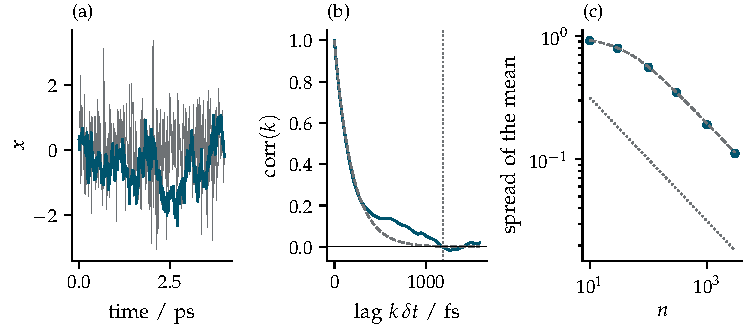
\includegraphics{ch15_convergence/ou}
\caption{Samples that remember: the series of \cref{eq:cv-ou} with $c =
0.95$, samples \SI{10}{\femto\second} apart. (a) 400 samples (teal)
against 400 independent ones (grey). (b) Its autocorrelation function
estimated from 10\,000 samples, against the exact $c^k$ (dashed); the
estimate first reaches zero at the dotted line. (c) The spread of the mean
of $n$ samples, 4000 series over, against $1/\sqrt n$ for independent
samples (dotted) and the square root of \cref{eq:cv-var} (dashed).}
\label{fig:cv-ou}
\end{figure}

\subsection*{Estimating $g$ from one run}

A run does not know its autocorrelation function and must estimate it.
With the deviations now taken from the run's own mean, $\delta A_i = A_i -
\bar A$ in place of $A_i - \ens{A}$, which the run does not know, and
$s'^2 = \frac1n\sum_i\delta A_i^2$, the estimate at the lag $k$ averages the
$n - k$ products available,
\begin{equation*}
   \widehat{\operatorname{corr}}(k)
   = \frac{1}{(n - k)\,s'^2}\sum_{i=1}^{n-k}\delta A_i\,\delta A_{i+k} ,
\end{equation*}
the hat marking an estimate. Each value carries noise, and beyond the
decay the estimates scatter about zero (\cref{fig:cv-ou}(b)): by 0.044
over the lags 300 to 1000 of 10\,000 samples of the series above, more
than $1/\sqrt n = 0.010$ because the products are themselves correlated.
Summed over every lag with the weights $1 - k/n$, the estimates give zero
in place of $g$, whatever the series. Multiplying out,
$(1 - k/n)\,\widehat{\operatorname{corr}}(k) = \sum_i\delta A_i\,\delta
A_{i+k}/(n s'^2)$, so
\begin{equation*}
   1 + 2\sum_{k=1}^{n-1}\Bigl(1 - \frac kn\Bigr)
   \widehat{\operatorname{corr}}(k)
   = \frac{\sum_i\delta A_i^2 + 2\sum_{k\ge1}\sum_i\delta A_i\,\delta
   A_{i+k}}{n s'^2}
   = \frac{\bigl(\sum_i\delta A_i\bigr)^2}{n s'^2} = 0 ,
\end{equation*}
the middle numerator being the square of the sum written out, and the
deviations from the run's own mean adding to zero. The sum must therefore
stop where the signal ends. The rule of Chodera and
co-workers\cite{Chodera2007} stops it where the estimate first reaches
zero; pymbar, and the listing below, look for that zero only beyond the
third lag. For the series of
\cref{fig:cv-ou}(b) that is the lag 119, \SI{1190}{\femto\second}, and $g$
comes out at 48.0 against the exact 39.0; over 200 such series the
estimate averages 41.6 and spreads by 8.7. From a run worth a few hundred
independent samples $g$ is uncertain by about a fifth, and the error bar,
which goes as $\sqrt g$, by about a tenth, since a small relative change
in $g$ changes $\sqrt g$ by half as much. The function
\texttt{statistical\_inefficiency} of \texttt{mdlab.analysis.stats}
applies the rule, with the autocorrelation function computed by the fast
Fourier transform for speed (a tool Chapter~16 explains); in it
\texttt{c} holds the estimates $\widehat{\operatorname{corr}}(k)$ at the
lags \texttt{k}:

\begin{code}
def statistical_inefficiency(series: ArrayLike, mintime: int = 3) -> float:
    a = np.asarray(series, dtype=float)
    n = len(a)
    if np.all(a == a[0]):
        raise ValueError("a constant series has no fluctuations")
    c = autocorrelation(a)[1 : n - 1]
    k = np.arange(1, n - 1)
    stop = np.nonzero((c <= 0) & (k > mintime))[0]
    end = stop[0] if len(stop) else len(c)
    g = 1 + 2 * np.sum(c[:end] * (1 - k[:end] / n))
    return float(max(g, 1.0))
\end{code}

\noindent It agrees with the same estimate in the \texttt{timeseries}
module of the pymbar package to nine figures (\texttt{test\_stats.py}).

\subsection*{The liquid}

The liquid of Chapter~13, followed for \SI{2}{\nano\second} under CSVR
with $\tau_{\mathrm T} = \SI{1}{\pico\second}$ and sampled every step,
shows two kinds of memory (\cref{fig:cv-acf}(a)). The potential energy,
the kinetic energy and the pressure lose part of their correlation within
\SI{0.1}{\pico\second}, as the atoms rattle against their neighbours:
$\operatorname{corr}$ is then 0.46, 0.63 and 0.66. The rest fades over
picoseconds, and sets $g$: 146 for $U$, 211 for $K$ and 188 for $P$, or
$\tau_{\mathrm{int}}$ of 0.73, 1.05 and \SI{0.94}{\pico\second}. The slow
part comes from the thermostat. At fixed energy, from the same liquid
(\cref{fig:cv-acf}(b)), $U$ and $K$, whose sum cannot change, have the
same function and $\tau_{\mathrm{int}} = \SI{77}{\femto\second}$, and $P$
has \SI{123}{\femto\second}. Under CSVR the total energy, which only the
thermostat changes, has $\tau_{\mathrm{int}} = \SI{1.71}{\pico\second}$,
close to the time $\tau_{\mathrm T}C_V/C_K = \SI{1.59}{\pico\second}$ over
which \cref{sec:th-berendsen} found a weak coupling to move the energy,
while the shear component $\mathsf{P}_{xy}$ of the pressure tensor, which
is not tied to the total energy, has \SI{0.18}{\pico\second} in both runs. The
length of run an average needs therefore depends on the thermostat as
well as on the liquid: a gentle coupling lets the energy wander slowly,
and every quantity tied to the energy inherits that slowness.

\begin{figure}[htb]
\centering
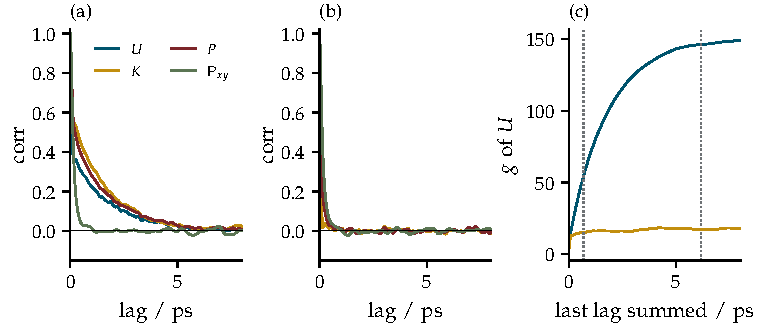
\includegraphics{ch15_convergence/acf}
\caption{The memory of liquid argon at \SI{135}{\kelvin}, from runs of
\SI{2}{\nano\second} sampled every \SI{10}{\femto\second}. (a) Under CSVR
with $\tau_{\mathrm T} = \SI{1}{\pico\second}$: the autocorrelation
functions of $U$, $K$, $P$ and the shear component $\mathsf{P}_{xy}$. (b)
The same at fixed energy, where $U$ and $K$ have the same function. (c)
The estimate of $g$ for $U$ summed up to each lag, under CSVR (teal) and
at fixed energy (ochre), with the lags at which the rule of this section
stops each sum (dotted).}
\label{fig:cv-acf}
\end{figure}

\Cref{fig:cv-acf}(c) shows the rule at work: under CSVR the running sum
for $U$ climbs until the estimate first reaches zero at \SI{6.16}{\pico
\second}, and at fixed energy it levels off before the sum stops at
\SI{0.70}{\pico\second}. Over the whole run under CSVR, the potential
energy of the 256 atoms is $U = (-12.8236 \pm
0.0047)$\,\si{\electronvolt}, $T = (134.81 \pm 0.22)$\,\si{\kelvin} and $P =
(0.0849 \pm 0.0004)$\,\si{\giga\pascal}. The error bars that leave out
$\sqrt g$, $s/\sqrt n$ over the 200\,001 samples, would be 12.1, 14.5 and
13.7 times smaller, and would claim a precision that the run does not
have.

\begin{keyidea}
Successive samples of a run are correlated, and $n$ of them spread the
mean as widely as $n/g$ independent ones, with the statistical
inefficiency $g = 1 + 2\sum_k\operatorname{corr}(k)$; a run of length
$t_{\mathrm f}$ holds $t_{\mathrm f}/(2\tau_{\mathrm{int}})$ independent
samples, $\tau_{\mathrm{int}} = g\dt/2$. The error of the mean is $\sqrt{g\,s^2/n}$, with $g$ estimated
from the run by summing its autocorrelation function until the estimate
first reaches zero.
\end{keyidea}

\notebook{15}{set the memory of a series and compare the naive and the
correct error bars}

\begin{selfcheck}
A series has $\operatorname{corr}(k) = 0.5^k$. What is $g$, and how many
independent samples are 1000 of its samples worth?
\end{selfcheck}

%=============================================================================!
% 15.3  BLOCK AVERAGES                                                        !
%=============================================================================!
\section{Block averages}
\label{sec:cv-blocks}

The estimate of $g$ rests on a rule for where the autocorrelation function
ends, and a slow tail that the rule cuts off would leave the error bar too
small. Block averaging finds the error of the mean without estimating the
autocorrelation function at all, and shows on a plot whether the run was
long enough to find it\cite{Flyvbjerg1989}.

\subsection*{Blocks of samples}

We cut the $n$ samples of a run into $n_{\mathrm b}$ consecutive blocks of
$b$ samples each, $n = n_{\mathrm b}b$ (a remainder at the end is dropped),
and average each block, giving the block means $\bar A_1, \dots, \bar
A_{n_{\mathrm b}}$, whose own mean is $\bar A$. Each block mean is the mean of
$b$ correlated samples, so by \cref{eq:cv-var} with $b$ in place of $n$ it
has the variance $g_b\sigma_A^2/b$, with
\begin{equation*}
   g_b = 1 + 2\sum_{k=1}^{b-1}\Bigl(1 - \frac kb\Bigr)
   \operatorname{corr}(k) .
\end{equation*}
Two neighbouring blocks share only the correlation between the samples
near their common edge, so blocks much longer than the run's memory have
nearly independent means. The mean of $n_{\mathrm b}$ independent block
means then has the variance of one divided by $n_{\mathrm b}$
(\cref{eq:cv-mean}), estimated from their own spread: the error of $\bar
A$ is $s_{\mathrm b}/\sqrt{n_{\mathrm b}}$, with $s_{\mathrm b}^2$ the sum of
the squared deviations of the block means from $\bar A$ divided by
$n_{\mathrm b} - 1$. No autocorrelation function enters.

How long the blocks must be follows from $g_b$. Splitting the sum,
\begin{equation*}
   g_b = 1 + 2\sum_{k=1}^{b-1}\operatorname{corr}(k)
   - \frac2b\sum_{k=1}^{b-1}k\operatorname{corr}(k)
   \approx g - \frac2b\sum_{k=1}^{\infty}k\operatorname{corr}(k) ,
\end{equation*}
since for blocks much longer than the memory both sums have already
reached their limits. For the exponential $\operatorname{corr}(k) = c^k$
of \cref{eq:cv-ou}, the second sum is $c/(1 - c)^2$ (\cref{ex:cv-ksum}),
which is $(g^2 - 1)/4$, since $g^2 - 1 = [(1 + c)^2 - (1 - c)^2]/(1 - c)^2
= 4c/(1 - c)^2$; for $g$ well above 1 it is close to $g^2/4$, so $g_b
\approx g - g^2/(2b)$. The blocks estimate the error
$\sqrt{g_b\sigma_A^2/(n_{\mathrm b}b)} = \sqrt{g_b\sigma_A^2/n}$, against
the true $\sqrt{g\sigma_A^2/n}$; the part missing is the correlation
between neighbouring blocks. Their ratio is $\sqrt{1 - x}$ with $x =
g/(2b)$, and a small relative change changes a square root by half as
much, so blocks of $b$ samples give an error too small by the fraction
\begin{equation}
   1 - \sqrt{g_b/g} \approx \frac{g}{4b} .
   \label{eq:cv-short}
\end{equation}
For the series with $g = 39$ the exact shortfall is 0.102 for $b = 100$
and 0.051 for $b = 195$, against 0.097 and 0.050 from \cref{eq:cv-short}.
Blocks of $5g$ samples miss about 5\% of the error when the memory is
exponential, a factor that the rest of the chapter uses. A memory that
falls quickly at first and then fades slowly, as the liquid's does
(\cref{fig:cv-acf}), has a larger $\sum_kk\operatorname{corr}(k)$ for the
same $g$, 1.7 to 2.0 times $(g/2)^2$ for $U$, $K$ and $P$, and blocks of
$5g$ samples then miss 0.107, 0.089 and 0.090 of the error, within the
error of an estimate from twenty blocks.

\subsection*{The plateau}

Flyvbjerg and Petersen double the block length at each stage, from 1
sample to as many as leave a few blocks, and plot the error against the
length\cite{Flyvbjerg1989}. Short blocks give the error of independent
samples, too small by $\sqrt g$; as the blocks grow past the memory the
estimate rises and levels off at $\sqrt{g\sigma_A^2/n}$. The level part is
the plateau, and its height is the error of the mean. Its own precision
is that of an estimate of a standard deviation from $n_{\mathrm b}$
samples: for nearly Gaussian block means the relative error of $s_{\mathrm
B}$ is $1/\sqrt{2(n_{\mathrm b} - 1)}$ (\cref{ex:cv-error-error}), 0.24 for
10 blocks and 0.16 for 20. The longest blocks, few in number, scatter.
The function \texttt{block\_average} of \texttt{mdlab.analysis.stats}
returns the error and its own error at each length:

\begin{code}
def block_average(series: ArrayLike, min_blocks: int = 4) -> dict:
    a = np.asarray(series, dtype=float)
    lengths, errors, error_errors, counts = [], [], [], []
    b = 1
    while len(a) // b >= min_blocks:
        n_b = len(a) // b
        means = a[: n_b * b].reshape(n_b, b).mean(axis=1)
        se = means.std(ddof=1) / np.sqrt(n_b)
        lengths.append(b)
        errors.append(se)
        error_errors.append(se / np.sqrt(2 * (n_b - 1)))
        counts.append(n_b)
        b *= 2
    return {"length": np.array(lengths), "error": np.array(errors),
            "error_error": np.array(error_errors),
            "blocks": np.array(counts)}
\end{code}

\noindent \Cref{fig:cv-blocks}(a) applies it to the series of
\cref{sec:cv-correlation}. With $2^{17}$ samples, 3361 independent ones,
the error rises from 0.0028 for single samples to a plateau of 0.0164 to
0.0168 for blocks of 256 to 1024 samples, against the exact 0.0172. With
$2^{10}$ samples, 26 independent ones, it rises to 0.182 for blocks of 64
and falls back to 0.131 for blocks of 256, of which only four remain,
while the exact value is 0.193: there is no plateau, and a run that shows
none is too short for its own error bar to be known. The criterion of
\cref{sec:cv-protocol} asks for at least 100 independent samples, enough
for twenty blocks of $5g$ samples and an error known to about a sixth.

\begin{figure}[htb]
\centering
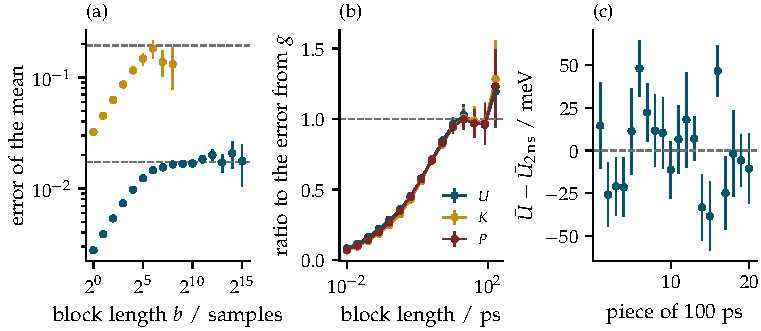
\includegraphics{ch15_convergence/blocks}
\caption{Block averages. (a) The series of \cref{eq:cv-ou} with $c =
0.95$: the error of the mean from blocks of $b$ samples, for $2^{17}$
samples (teal) and $2^{10}$ (ochre), with the error of each estimate,
against the exact errors (dashed). (b) The liquid under CSVR, \SI{2}{\nano
\second}: the error of the mean of $U$, $K$ and $P$ from blocks, divided by
$\sqrt{g s^2/n}$. (c) The same run cut into twenty runs of
\SI{100}{\pico\second}: the mean of $U$ in each, less that of the whole
run, with its own error bar from that piece alone.}
\label{fig:cv-blocks}
\end{figure}

\subsection*{The liquid, and a test against independent runs}

For the liquid of \cref{fig:cv-acf}, blocks of \SI{20}{\pico\second} give
1.03, 1.01 and 1.00 times the errors found from $g$ for $U$, $K$ and $P$,
and blocks of \SI{41}{\pico\second} 0.98, 0.99 and 0.97
(\cref{fig:cv-blocks}(b)): the rule of \cref{sec:cv-correlation} missed no
slow tail that blocks known to 7\% could show. The longest blocks,
\SI{164}{\pico\second} and only twelve of them, give 1.20 to 1.28, about
one of their own errors, a fifth, above 1.

The sharper test is whether an error bar from one run predicts how far
other runs fall from it. Cutting the \SI{2}{\nano\second} run into twenty
pieces of \SI{100}{\pico\second}, whose means are nearly independent
(successive means have the correlation 0.06), gives twenty runs to set
against one another (\cref{fig:cv-blocks}(c)). Their means of $U$ scatter
by \SI{0.0241}{\electronvolt}, while the error bar that each piece finds
for itself averages \SI{0.0196}{\electronvolt}, from 0.0128 to
\SI{0.0278}{\electronvolt}; for $K$ the figures are 0.0351 and
\SI{0.0312}{\electronvolt}, and for $P$ 0.00201 and
\SI{0.00172}{\giga\pascal}. Eleven of the twenty bars for $U$ hold the mean
of the whole run, where one standard error should hold it in 68\% of
runs, 13.7 of twenty on average, a count that itself spreads by 2.1, since
each piece holds the mean or not, a yes or no of variance $0.68\times0.32$,
and the twenty variances add. A piece of \SI{100}{\pico\second} holds 68
independent samples of $U$, and the $g$ it finds for itself ranges from 64
to 228, on either side of the 146 of the whole run: an error bar from so
short a run is uncertain by about a fifth (the twenty bars for $U$ spread
by 0.20 of their mean), and on average a little low.

\begin{keyidea}
Block means of blocks much longer than the run's memory are nearly
independent, and their spread gives the error of the mean with no
autocorrelation function. Plotted against the block length, the error
rises to a plateau; blocks of $5g$ samples miss about 5\% of it for an
exponential memory, and the
plateau's own relative error is $1/\sqrt{2(n_{\mathrm b} - 1)}$. A run
with no plateau is too short to know its error bar.
\end{keyidea}

\notebook{15}{cut a series into blocks and find the plateau}

\begin{selfcheck}
A run of 20\,000 samples has $g = 100$ and an exponential memory. How long
must its blocks be to miss about 5\% of the error, and how many such
blocks does the run hold?
\end{selfcheck}

%=============================================================================!
% 15.4  WHERE A RUN BEGINS                                                    !
%=============================================================================!
\section{Where a run begins}
\label{sec:cv-equilibration}

A run starts from positions and velocities that the ensemble would rarely
produce: a lattice for a liquid, a box of the wrong volume, a structure
just built. Its early part relaxes towards the ensemble, and an average
that includes it is shifted however long the run. This section finds how
large that shift is, and how to choose the start of the part to keep.

\subsection*{A cup of coffee}

Hot coffee left on a table cools at a rate proportional to how much
warmer than the room it is: $\dd T/\dd t = -(T - T_{\mathrm{room}})/\tau_{\mathrm r}$,
with $\tau_{\mathrm r}$ set by the cup and the air. This is the decay
equation of \cref{sec:ne-drag} for $T - T_{\mathrm{room}}$, with
$1/\tau_{\mathrm r}$ in place of $\gamma$, so
\begin{equation*}
   T(t) = T_{\mathrm{room}} + \bigl(T(0) - T_{\mathrm{room}}\bigr)
   \mathrm{e}^{-t/\tau_{\mathrm r}} .
\end{equation*}
A thermometer in the cup, read from the moment the coffee is poured and
averaged, gives a temperature above the room's. A run behaves the same
way: a quantity $A$ approaches its ensemble average with a decaying offset
$\delta A_0\,\mathrm{e}^{-t/\tau_{\mathrm r}}$, which is $\delta A_0$ at the
start, and on which the run's own
fluctuations ride. Averaged over a run of length $t_{\mathrm f}$ from its
start, the offset contributes
\begin{equation*}
   \frac{1}{t_{\mathrm f}}\int_0^{t_{\mathrm f}}\delta A_0\,
   \mathrm{e}^{-t/\tau_{\mathrm r}}\,\dd t
   = \frac{\delta A_0\,\tau_{\mathrm r}}{t_{\mathrm f}}\Bigl[-\mathrm{e}^{-t/
   \tau_{\mathrm r}}\Bigr]_0^{t_{\mathrm f}}
   = \frac{\delta A_0\,\tau_{\mathrm r}}{t_{\mathrm f}}\bigl(1 -
   \mathrm{e}^{-t_{\mathrm f}/\tau_{\mathrm r}}\bigr)
   \approx \frac{\delta A_0\,\tau_{\mathrm r}}{t_{\mathrm f}}
\end{equation*}
for a run much longer than $\tau_{\mathrm r}$. The shift falls as
$1/t_{\mathrm f}$ and the error bar as $1/\sqrt{t_{\mathrm f}}$, so a long
enough run would hide the shift inside its error bar, but only slowly.
Leaving out the first $t_0$ of the run cuts the offset's share to
$\delta A_0\,\tau_{\mathrm r}\mathrm{e}^{-t_0/\tau_{\mathrm r}}/(t_{\mathrm f}
- t_0)$ (\cref{ex:cv-offset}), at the cost of the samples discarded.

\subsection*{The start that leaves the most}

Discarding too little leaves a shift; discarding too much throws away
samples. Chodera found a way to weigh the two from the run
alone\cite{Chodera2016}. To the autocorrelation function a decaying offset
looks like a very slow correlation, and it inflates $g$; so for each
candidate start $t_0$, the effective number of samples left after it,
\begin{equation*}
   n_{\mathrm{eff}}(t_0) = \frac{n - t_0/\dt}{g(t_0)} ,
\end{equation*}
with $t_0/\dt$ the number of samples discarded and $g(t_0)$ the
statistical inefficiency of the samples from $t_0$ on,
rises while the discard removes more of the offset's inflation of $g$
than it costs in samples, and falls once only samples are being removed.
The start kept is the one that maximises it:

\begin{code}
def detect_equilibration(
    series: ArrayLike, nskip: int = 1
) -> tuple[int, float, float]:
    a = np.asarray(series, dtype=float)
    n = len(a)
    best = (0, 1.0, 0.0)
    for t0 in range(0, n - 1, nskip):
        rest = a[t0:]
        if np.all(rest == rest[0]):
            g = float(n - t0)
        else:
            g = statistical_inefficiency(rest)
        if (n - t0) / g > best[2]:
            best = (t0, g, (n - t0) / g)
    return best
\end{code}

\noindent The listing counts \texttt{t0} in samples. It finds the same
start as the function of the same name in the \texttt{timeseries} module
of pymbar with \texttt{fast=False} (\texttt{test\_stats.py}); pymbar's
default estimates $g$ more roughly and can place the start a few samples
later, 550 against 534 for the series below.

\Cref{fig:cv-equilibration}(a) adds the offset $3\,\mathrm{e}^{-t/\SI{2}{\pico
\second}}$, three standard deviations at the start, to \SI{50}{\pico
\second} of the series of \cref{sec:cv-correlation}, and (b) shows
$n_{\mathrm{eff}}(t_0)$ rising to 158 at \SI{5.34}{\pico\second}, 2.7 decay
times, and falling after. From the start the mean is $0.160 \pm 0.164$,
of which the offset contributes $\delta A_0\,\tau_{\mathrm r}/t_{\mathrm f} = 0.120$; after
the discard it is $0.001 \pm 0.076$, the offset contributing 0.0093, and
the error bar has halved. One series is one draw: over 200 such series the
start falls between 0.1 and 16.5 decay times, with the median, the value
with half the series on either side, at 1.4, and
the offset left in the mean is at most 1.35 error bars, with the median
0.34. One error bar then holds the true mean in 0.58 of the series, where
it should hold it in 0.68; without the discard, in 0.54. The method trades
a shift of about a third of an error bar for an error bar half as large,
and leaves part of a slow offset in place, which the test for drift of
\cref{sec:cv-drift} looks for.

\begin{figure}[htb]
\centering
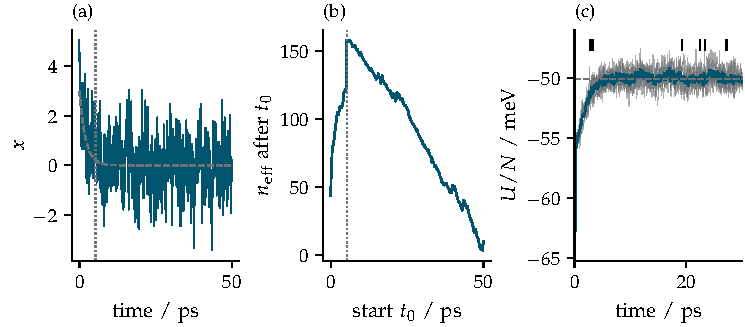
\includegraphics{ch15_convergence/equilibration}
\caption{Where a run begins. (a) \SI{50}{\pico\second} of the series of
\cref{eq:cv-ou} with $c = 0.95$, with the offset $3\,\mathrm{e}^{-t/\SI{2}{\pico
\second}}$ added, the offset itself dashed, and the start found (dotted).
(b) The effective number of samples after each candidate start,
maximised at the dotted line. (c) The first \SI{30}{\pico\second} of eight
runs of the liquid melting from the face-centred
cubic lattice at \SI{135}{\kelvin}: the potential energy per atom (grey),
their mean (teal) and the mean of the \SI{2}{\nano\second} run (dashed),
with the start found in each run from its own $U$ (ticks).}
\label{fig:cv-equilibration}
\end{figure}

\subsection*{A liquid melting}

\Cref{fig:cv-equilibration}(c) starts eight runs of the liquid from the
face-centred cubic lattice at the liquid's density, with velocities drawn
at \SI{135}{\kelvin} from eight seeds, under CSVR for \SI{100}{\pico
\second}. The lattice has $U/N = \SI{-64.331}{\milli\electronvolt}$; the
energy climbs from it as the lattice melts, and the mean of the eight runs
comes
within \SI{1}{\milli\electronvolt} of the \SI{2}{\nano\second} run's
$(-50.092 \pm 0.018)$\,\si{\milli\electronvolt} after \SI{2.89}{\pico
\second}. In four of the runs the start found from $U$ is 2.8 to
\SI{3.2}{\pico\second}, at the end of the melting. In the other four it is
19 to \SI{27}{\pico\second}: under CSVR the energy wanders over
picoseconds (\cref{sec:cv-correlation}), and a run of \SI{100}{\pico
\second} cannot always tell such a wander from the tail of a transient.
Discarding more than needed costs samples and, on average, does not shift
the mean.
Averaged from their first steps, the eight means of $U/N$ lie at $-50.169$
on average, the melting's share pulling them down; after the discards
they average \SI{-50.063}{\milli\electronvolt}, close to the
\SI{2}{\nano\second} value, and scatter by \SI{0.111}{\milli\electronvolt}
against error bars of 0.046 to \SI{0.085}{\milli\electronvolt}, 0.067 on
average. The error bars are low by about two fifths, though a spread from
eight runs is itself uncertain by a quarter (\cref{ex:cv-error-error}). A
run of \SI{100}{\pico\second} holds about 68 independent samples of $U$
(\cref{sec:cv-blocks}), and the start chosen makes $(n - t_0/\dt)/g(t_0)$
largest, which favours a start after which $g$ happens to come out small:
the eight runs find $g$ of 45 to 138 after their starts, against the 146
of the \SI{2}{\nano\second} run, and their error bars are small with it.

The same holds for any quantity with few independent samples.
Chapter~14's three runs of \SI{300}{\pico\second} at constant pressure
under stochastic cell rescaling hold 35, 73 and 109 independent samples of
the volume. In the second and third the start found is 1.0 and
\SI{0.0}{\pico\second}, well within the first \SI{10}{\pico\second} that
\cref{sec:pr-trajectory} left out of its averages. In the first,
$n_{\mathrm{eff}}(t_0)$ falls from 35 at the start, as a settled run's
should, to 24 at \SI{100}{\pico\second} and 9 at \SI{195}{\pico\second};
beyond, the $g$ estimated from the last few tens of picoseconds is so
uncertain that it can come out far too small, and the largest value, 55,
falls at \SI{259}{\pico\second}, a start with no meaning. The criterion of \cref{sec:cv-protocol}
therefore asks that the start lie in the first half of the run. Chapter~11
prepared its water in rounds of \SI{1}{\pico\second} and left the end of
that slow change unmeasured (\cref{sec:cs-water}); its healthy run of
\SI{10}{\pico\second} at fixed energy has its start at \SI{0.30}{\pico
\second}, after which the box's kinetic energy is $K = (4.993 \pm
0.022)$\,\si{\electronvolt} and the potential energy $(-0.40265 \pm
0.00034)$\,\si{\electronvolt} per molecule, against 4.990 and $-0.40259$
over the whole run: the preparation had all but finished, and
the averages that \cref{sec:cs-trajectory} quoted stand within their error
bars.

\begin{keyidea}
A run's early part relaxes from its start, and shifts the mean of the
whole run by about $\delta A_0\,\tau_{\mathrm r}/t_{\mathrm f}$. The start to keep is the
one that leaves the largest effective number of samples, $(n - t_0/\dt)/
g(t_0)$. The method trades a shift of a fraction of an error bar for
precision and needs a
run with many independent samples: when the start it finds falls in the
second half of the run, the run is too short to locate it.
\end{keyidea}

\notebook{15}{add a transient of your choosing and watch where the start
is found}

\begin{selfcheck}
A run of \SI{100}{\pico\second} has an offset of \SI{2}{\kelvin} in its
temperature at the start, decaying with the time $\tau_{\mathrm r} =
\SI{1}{\pico\second}$. By how much
does it shift the mean temperature of the whole run?
\end{selfcheck}

%=============================================================================!
% 15.5  A SLOW DRIFT                                                          !
%=============================================================================!
\section{A slow drift}
\label{sec:cv-drift}

A run can settle and still not hold still. An integration step that is too
long lets the total energy creep, a thermostat set to the wrong target
moves the temperature slowly, and a transient that discarding the start
found in \cref{sec:cv-equilibration} did not remove leaves a slow slope. Each is a
trend under the fluctuations, and this section fits a straight line to a
run to find it, with an error that accounts for the run's memory.

\subsection*{A tyre that may be leaking}

A bicycle tyre is checked with a gauge every morning for a month. The
gauge scatters by \SI{0.05}{bar} from reading to reading, and a slow leak
of \SI{0.01}{bar} a day hides under that scatter from one day to the
next, but not over thirty days. The straight line that passes closest to
the thirty readings finds it, and the toolbox gives that line and the
error of its slope.

\begin{toolbox}[A straight line through scattered points]
Readings $A_i$ at the times $t_i$, $i = 1, \dots, n$, are to be described by
$A \approx a + \dot A\,(t - \bar t)$, with $\bar t$ the mean time. The line
of least squares chooses $a$ and the slope $\dot A$ to make the sum of
squared misses $S_{\mathrm m} = \sum_i\bigl[A_i - a - \dot A(t_i - \bar
t)\bigr]^2$ as small as it can be, where its rates of change with $a$ and
with $\dot A$ both vanish. With respect to $a$,
\begin{equation*}
   \frac{\partial S_{\mathrm m}}{\partial a} = -2\sum_i\bigl[A_i - a - \dot A(t_i -
   \bar t)\bigr] = -2\Bigl(n\bar A - na - \dot A\cdot0\Bigr) = 0 ,
\end{equation*}
since the deviations $t_i - \bar t$ add to zero, so $a = \bar A$. With
respect to $\dot A$, multiplying each miss by $t_i - \bar t$,
\begin{equation*}
   \frac{\partial S_{\mathrm m}}{\partial\dot A} = -2\sum_i(t_i - \bar t)\bigl[A_i -
   \bar A - \dot A(t_i - \bar t)\bigr] = 0 , \qquad
   \dot A = \frac{\sum_i(t_i - \bar t)(A_i - \bar A)}{S_{tt}} ,
\end{equation*}
with $S_{tt} = \sum_i(t_i - \bar t)^2$. The slope is a weighted sum of the
readings, $\dot A = \sum_iw_iA_i$ with $w_i = (t_i - \bar t)/S_{tt}$, since
$\sum_iw_i\bar A = 0$. If the misses about the true line are independent
with variance $\sigma_{\mathrm m}^2$, the variances of the terms add, and a
constant factor $w_i$ multiplies a variance by $w_i^2$
(\cref{sec:cv-mean}), so
\begin{equation*}
   \operatorname{var}(\dot A) = \sigma_{\mathrm m}^2\sum_iw_i^2
   = \frac{\sigma_{\mathrm m}^2}{S_{tt}^2}\sum_i(t_i - \bar t)^2
   = \frac{\sigma_{\mathrm m}^2}{S_{tt}} .
\end{equation*}
$\sigma_{\mathrm m}^2$ is estimated from the misses about the fitted line, their sum
of squares divided by $n - 2$, since two quantities have been fitted to
the same readings; for the thousands of samples of a run the difference
from $n$ is negligible.
\end{toolbox}

For thirty daily readings $S_{tt} = \SI{2247.5}{\day\squared}$, so the
slope is known to $0.05/\sqrt{2247.5} = 0.00105$\,bar a day. One
month of readings drawn by computer with the leak gives $\dot A =
(-0.0109 \pm 0.0012)$\,bar a day, nine errors from zero (the
misses of this month scatter by \SI{0.057}{bar}, hence 0.0012 rather than
0.00105): the leak is certain, though no single day shows it.

\subsection*{The slope of a correlated series}

The samples of a run are correlated, and so are their misses about the
line. The variance of the weighted sum is then, as in
\cref{sec:cv-correlation}, a double sum over pairs,
\begin{equation*}
   \operatorname{var}(\dot A) = \sigma_{\mathrm m}^2\sum_i\sum_jw_iw_j
   \operatorname{corr}(\lvert i - j\rvert)
   \approx \sigma_{\mathrm m}^2\sum_iw_i^2\Bigl[1 +
   2\sum_{k\ge1}\operatorname{corr}(k)\Bigr]
   = \frac{g\,\sigma_{\mathrm m}^2}{S_{tt}} ,
\end{equation*}
the approximation taking $w_j = w_i$ wherever $\operatorname{corr}$ is not
negligible, which holds when the run is much longer than its memory: across
a memory of about $g$ samples a weight changes by $g\dt/S_{tt}$, a fraction
$2g/n$ of the largest weight, $(t_{\mathrm f}/2)/S_{tt}$. The slope's
error carries the same factor $\sqrt g$ as the mean's, with $g$ found from
the misses. For $n$ samples evenly spaced by $\dt$, $S_{tt} = n(n^2 -
1)\dt^2/12$ (\cref{ex:cv-stt}), close to $nt_{\mathrm f}^2/12$ for a run
of length $t_{\mathrm f} = n\dt$, so with $\tau_{\mathrm{int}} = g\dt/2$,
\begin{equation*}
   \operatorname{var}(\dot A) \approx
   \frac{12\,g\,\sigma_{\mathrm m}^2\dt}{t_{\mathrm f}^3}
   = \frac{24\,\sigma_{\mathrm m}^2\tau_{\mathrm{int}}}{t_{\mathrm f}^3} :
\end{equation*}
the error of a slope falls as $t_{\mathrm f}^{-3/2}$, and a run four times
as long can detect a slope eight times smaller. The ratio of the slope to
its error then tests for a drift: for a series with none it is Gaussian
with unit spread, and lies beyond $\pm2$ in 4.6\% of runs
(\cref{sec:sm-probability}). Applied to 1000 series of 5000 samples of the
kind in \cref{fig:cv-ou}, with $g = 39$ and no drift, the
test \texttt{drift\_test} of \texttt{mdlab.analysis.stats} finds a drift
in 0.051 of them. A slope beyond two errors is evidence of drift worth investigating; within them, the run shows none that it can detect.

\subsection*{The time step}

Chapter~9 judged a time step by the spread of the total energy at fixed
energy, which should fall as $\dt^2$ and stay small beside the spread of
the kinetic energy, and by the absence of a drift (\cref{sec:in-stability}).
The drift test makes the last of these quantitative.
\Cref{fig:cv-drift} follows the liquid at fixed energy for
\SI{1}{\nano\second} at each of six steps. The spread of the total energy
over that of the kinetic energy is 3.93 times larger at 10 than at
\SI{5}{\femto\second} and 4.12 times larger at 20 than at
\SI{10}{\femto\second}, the factor 4 of $\dt^2$, but 3.93 times larger at
30 than at \SI{20}{\femto\second}, where $\dt^2$ gives 2.25, and 6.18 times
larger at 35 than at \SI{30}{\femto\second}, where it gives 1.36: beyond
\SI{20}{\femto\second} the step is leaving the range in which its error is
a small, smooth correction. The drift per atom per nanosecond is $0.00
\pm 0.01$ and $-0.04 \pm 0.05$\,\si{\micro\electronvolt} at 5 and
\SI{10}{\femto\second}; $-0.66 \pm 0.17$\,\si{\micro\electronvolt} at
\SI{20}{\femto\second}; $-54 \pm 29$\,\si{\micro\electronvolt} at
\SI{30}{\femto\second}; $+642 \pm 69$\,\si{\micro\electronvolt} at
\SI{35}{\femto\second}; and at \SI{40}{\femto\second} the energy climbs by
\SI{11}{\milli\electronvolt} per atom per nanosecond over the
\SI{363}{\pico\second} it takes to gain \SI{1}{\electronvolt} in all, and
the run blows up at \SI{557}{\pico\second}.

Whether a drift matters depends on what the run measures. At fixed energy
a drift $\dot E$ moves the temperature at the rate $\dot E/C_V$, and over
a run of length $t_{\mathrm f}$ moves its mean by half of $\dot
Et_{\mathrm f}/C_V$. Asking that this be smaller than the mean's own error
$\sigma_{\bar T}$,
\begin{equation*}
   \frac{\lvert\dot E\rvert}{N} < \frac{2\sigma_{\bar T}}{t_{\mathrm f}}\,
   \frac{C_V}{N} .
\end{equation*}
For this liquid $C_V/N = 2.347\kB$, the mean of the five single-run
estimates of \cref{sec:sm-kinetic} (the slope of $E$ against $T$ gives
2.376, within the 3\% errors of those runs, \cref{sec:cv-observables}), and $\sigma_{\bar T} =
\SI{0.0513}{\kelvin}$ over \SI{1}{\nano\second} at fixed
energy, so the limit for a run of \SI{1}{\nano\second} is
\SI{20.8}{\micro\electronvolt} per atom per nanosecond (dotted in
\cref{fig:cv-drift}(b)). The drift at \SI{20}{\femto\second} is significant,
3.8 errors from zero, and harmless: it moves the temperature by
\SI{0.0033}{\kelvin} in a nanosecond. The drift at \SI{30}{\femto\second}
lies 1.8 errors from zero and 1.1 above the limit, so the run can show it
neither significant nor harmful; at \SI{35}{\femto\second} it moves the
temperature by \SI{3.2}{\kelvin} per nanosecond. Significance grows with the length of a run, which can detect
ever smaller drifts; importance is set by the quantity measured. For this liquid \SI{20}{\femto\second} passes Chapter~9's tests
of the spread, and its drift, though significant, is harmless for a run of
\SI{1}{\nano\second} and at the limit for one of \SI{10}{\nano\second}
(\cref{ex:cv-drift-limit}); \SI{10}{\femto\second}, the step used
throughout, passes them with a wide margin and shows no drift the test can
detect.

\begin{figure}[htb]
\centering
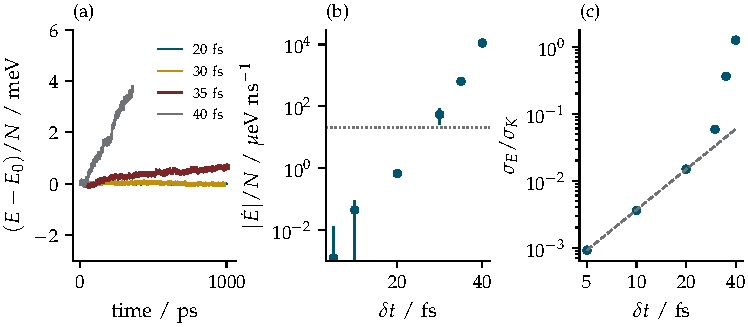
\includegraphics{ch15_convergence/drift}
\caption{A slow drift: the liquid at fixed energy for \SI{1}{\nano\second}
at each step. (a) The total energy per atom less its start, at 20 (teal),
30 (ochre), 35 (oxblood) and \SI{40}{\femto\second} (grey, until it passes
\SI{1}{\electronvolt} in all). (b) The size of the drift per atom per
nanosecond, with its error, against the step, and the largest drift that
moves the mean temperature of a \SI{1}{\nano\second} run by less than its
error (dotted). (c) The spread of the total energy over that of the
kinetic energy, against $\dt^2$ through the point at \SI{5}{\femto\second}
(dashed).}
\label{fig:cv-drift}
\end{figure}

\begin{keyidea}
A drift is the slope of the line of least squares through a run, with the
error $\sqrt{g\sigma_{\mathrm m}^2/S_{tt}}$ that the run's memory requires; a slope
beyond two errors is evidence of drift under this test. Whether it matters depends on what is
measured: at fixed energy it is harmless while it moves the mean
temperature by less than its error. A step is acceptable while the
energy's spread grows as $\dt^2$ and its drift is harmless.
\end{keyidea}

\notebook{15}{hide a leak under noise and test for it}

\begin{selfcheck}
A run of \SI{500}{\pico\second} gives a drift of $(3 \pm 2)$ in some unit.
Is it a drift, and what would a run of \SI{2}{\nano\second} with the same
true slope be expected to show?
\end{selfcheck}

%=============================================================================!
% 15.6  HOW LONG FOR EACH QUANTITY                                            !
%=============================================================================!
\section{How long for each quantity}
\label{sec:cv-observables}

Each quantity of a run has its own spread and its own memory, so each
needs its own length of run for a given precision. This section measures
both for the liquid, turns them into run lengths, and settles with error
bars the questions that Chapters~12 to 14 left open.

\subsection*{The length of run for a precision}

With $n_{\mathrm{eff}} = t_{\mathrm f}/(2\tau_{\mathrm{int}})$ independent
samples in a run of length $t_{\mathrm f}$ (\cref{sec:cv-correlation}), the
error of the mean is $\sigma_A\sqrt{2\tau_{\mathrm{int}}/t_{\mathrm f}}$.
Asking for an error no larger than a target $\sigma^\ast$ and solving for
$t_{\mathrm f}$,
\begin{equation}
   t_{\mathrm f} \ge \frac{2\tau_{\mathrm{int}}\,\sigma_A^2}{\sigma^{\ast2}} :
   \label{eq:cv-length}
\end{equation}
twice the correlation time for each of the $(\sigma_A/\sigma^\ast)^2$
independent samples needed. Halving the error costs four times
the run. \Cref{fig:cv-observables}(a) checks the $t_{\mathrm f}^{-1/2}$ on the
\SI{2}{\nano\second} run cut into pieces of 50 to \SI{2000}{\pico\second}:
for $U$ the means of the pieces spread by 6.77, 5.14 and 3.36 times the
error of the whole run for pieces of 50, 100 and \SI{200}{\pico\second},
against $\sqrt{40} = 6.32$, $\sqrt{20} = 4.47$ and $\sqrt{10} = 3.16$. The
error bar that each piece finds for itself is lower, 5.38 and 4.19 for the
two shortest,
as \cref{sec:cv-blocks} found, and meets the line from
\SI{200}{\pico\second} on.

\Cref{tab:cv-observables} gives the spread, the correlation time and the
run needed for a stated precision, from \cref{eq:cv-length}, for the
quantities of the liquid. Two things stand out. The pressure has a spread
of \SI{0.0133}{\giga\pascal} per sample about a mean of
\SI{0.085}{\giga\pascal}, a sixth of its value, so with a memory like that
of $U$ and $T$ its mean is slow to fix relative to its size:
\SI{1}{\nano\second} fixes it to 0.7\%, against 0.05\% for $U$. And the
runs at fixed energy need a 15th to a 38th of the time needed under CSVR
for the same precision of $U$, $T$ and $P$, because their correlation
times are 8 to 14 times shorter (\cref{sec:cv-correlation}) and their
spreads smaller. A run at fixed energy samples the microcanonical
ensemble, at the temperature its energy fixes: here \SI{133.70}{\kelvin},
\SI{1.1}{\kelvin} below the CSVR run, because the energy it was given is
the mean of \SI{40}{\pico\second} of CSVR, which, with the
\SI{1.71}{\pico\second} memory of the energy, is uncertain by about
\SI{1.6}{\kelvin} of temperature.
\Cref{sec:th-compare} recommended preparing a run under a thermostat and
gathering its dynamical quantities at fixed energy; for averages too,
fixed energy reaches a precision sooner, at the temperature its energy
sets.

\begin{table}[htb]
\centering
\small
\caption{How long each quantity needs, for liquid argon at
\SI{135}{\kelvin}: the spread of one sample, the integrated correlation
time under CSVR with $\tau_{\mathrm T} = \SI{1}{\pico\second}$ and at fixed
energy, the error of the mean after \SI{1}{\nano\second} under CSVR, and
the run needed for the target error $\sigma^\ast$, from
\cref{eq:cv-length}. The
volume is from Chapter~14's runs under stochastic cell rescaling at
\SI{0.1}{\giga\pascal}; $D$ from blocks of \SI{100}{\pico\second}.}
\label{tab:cv-observables}
\begin{tabular}{@{}lccccccc@{}}
\toprule
& spread & \multicolumn{2}{c}{$\tau_{\mathrm{int}}$ / ps} & error of
& target & \multicolumn{2}{c}{run / ns}\\
& CSVR / fixed $E$ & CSVR & fixed $E$ & \SI{1}{\nano\second} &
$\sigma^\ast$ & CSVR & fixed $E$\\
\midrule
$U/N$ & \SI{0.677}{\milli\electronvolt} / 0.532 & 0.73 & 0.077 &
\SI{0.026}{\milli\electronvolt} & \SI{0.01}{\milli\electronvolt} & 6.7 & 0.44\\
$T$ & \SI{6.93}{\kelvin} / 4.13 & 1.05 & 0.077 & \SI{0.32}{\kelvin} &
\SI{0.1}{\kelvin} & 10 & 0.26\\
$P$ & \SI{0.0133}{\giga\pascal} / 0.0096 & 0.94 & 0.123 &
\SI{0.00058}{\giga\pascal} & \SI{0.001}{\giga\pascal} & 0.33 & 0.023\\
$\mathsf{P}_{xy}$ & \SI{0.0121}{\giga\pascal} & 0.18 & 0.18 & & & &\\
$V$ & \SI{185}{\angstrom\cubed} & 2.5 & & \SI{13}{\angstrom\cubed} &
\SI{10}{\angstrom\cubed} & 1.7 &\\
$D$ & & & & 1.0\% & 1\% & 1.0 &\\
\bottomrule
\end{tabular}
\end{table}

\subsection*{Diffusion under a thermostat}

Chapter~13 found the diffusion coefficient under CSVR, Nosé-Hoover chains
and Berendsen coupling 1.01 to 1.07 times its value at fixed energy, in
runs 0.4 to \SI{1.8}{\kelvin} warmer, and left open whether the difference
was real (\cref{sec:th-compare}). Cutting each run of this chapter into
blocks of \SI{100}{\pico\second}, long beside the \SI{20}{\pico\second}
over which $D$ is fitted, gives independent estimates whose spread gives
the error. The \SI{2}{\nano\second} run under CSVR has $D = (3.877 \pm
0.028)\times10^{-4}$\,\si{\angstrom\squared\per\femto\second} at $(134.81
\pm 0.22)$\,\si{\kelvin}; the \SI{2}{\nano\second} run at fixed energy has
$(3.834 \pm 0.034)\times10^{-4}$ at \SI{133.70}{\kelvin}. The two are at
different temperatures, and runs under CSVR at 130 and \SI{140}{\kelvin}
give the slope $\dd D/\dd T = (0.0294 \pm 0.0071)\times10^{-4}$\,\si{\angstrom
\squared\per\femto\second\per\kelvin}
(\cref{fig:cv-observables}(b)). Moved along it to \SI{134.81}{\kelvin},
the run at fixed energy gives $(3.867 \pm 0.035)\times10^{-4}$, and the
ratio of the two is $1.002 \pm 0.011$. Berendsen coupling with
$\tau_{\mathrm T} = \SI{0.1}{\pico\second}$ at 130 and \SI{140}{\kelvin}
lies 1.3 and 0.3 errors from the line through the CSVR runs. To about 2\%,
CSVR with $\tau_{\mathrm T} = \SI{1}{\pico\second}$ and Berendsen coupling
with $\tau_{\mathrm T} = \SI{0.1}{\pico\second}$ leave diffusion alone.
Chapter~13 found $1.05 \pm 0.01$ and $1.04 \pm 0.01$ for these two from
three runs of \SI{100}{\pico\second} each. A block of
\SI{100}{\pico\second} here fixes $D$ to 3.2\%, so a mean of three such
runs is uncertain by $3.2/\sqrt3 = 1.8\%$ and a ratio of two such means
by $1.8\times\sqrt2 = 2.6\%$: the two values lie within about two such
errors of 1 once their warmth is removed, and the $\pm0.01$ came from the
spread of only three runs, itself uncertain by half
(\cref{ex:cv-error-error}). The other couplings of Chapter~13 were not run
again.

\begin{figure}[htb]
\centering
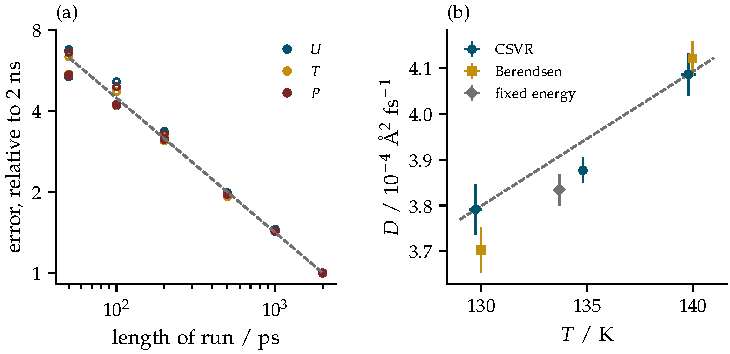
\includegraphics{ch15_convergence/observables}
\caption{(a) The error of the mean of $U$, $T$ and $P$ against the length
of run: the \SI{2}{\nano\second} CSVR run cut into pieces, the error bar
each piece finds for itself averaged over the pieces (filled) and the
spread of the pieces' means (open), each divided by the error of the whole
run, against the inverse square root of the length (dashed). (b) The
diffusion coefficient against
the temperature, with errors from blocks of \SI{100}{\pico\second}: CSVR
(teal), Berendsen coupling with $\tau_{\mathrm T} = \SI{0.1}{\pico\second}$
(ochre) and fixed energy (grey), with the line through the CSVR runs at
130 and \SI{140}{\kelvin} (dashed).}
\label{fig:cv-observables}
\end{figure}

\subsection*{Questions left open}

Chapter~12 found the light atoms of a mixture at \SI{126}{\kelvin} and
the heavy at \SI{124}{\kelvin} over the last \SI{10}{\pico\second} of a run,
and asked whether the gap was real (\cref{sec:sm-equipartition}). Taking
the difference of the two temperatures at each recorded frame as the
series, its mean is $(1.30 \pm 2.14)$\,\si{\kelvin}, with $g = 31.4$: 0.6
errors from zero, and equipartition between the species holds within what
the run can tell. Chapter~12 also found single runs of \SI{50}{\pico\second}
at fixed energy to give heat capacities scattered by up to 7.5\% about the
slope of $E$ against $T$, $2.376\,N\kB$ (\cref{sec:sm-kinetic}); the five
runs of 256 atoms lie within 5.3\% of it, and the 7.5\% is a run of 864
atoms. A heat capacity comes from a variance, whose error the rule for a
mean does not give; it is found by resampling, which \cref{sec:cv-ensemble}
sets out. It gives the five runs of 256 atoms errors of 2.9 to 3.9\%,
$(2.292 \pm 0.067)\,N\kB$ near \SI{130}{\kelvin} among them, and all five
lie within 1.7 of their errors of the slope: their scatter was the noise
of the runs.
Chapter~14 quoted the pressure of the liquid as \SI{0.0877}{\giga\pascal}
(\cref{sec:pr-periodic}), from 50 frames \SI{2}{\pico\second} apart,
farther apart than $2\tau_{\mathrm{int}} = \SI{1.9}{\pico\second}$, so
nearly independent: its error is
$0.0133/\sqrt{50} = \SI{0.0019}{\giga\pascal}$. The \SI{2}{\nano\second}
run gives $(0.0849 \pm 0.0004)$\,\si{\giga\pascal}, 1.4 combined errors
away.

\begin{keyidea}
A run of length $t_{\mathrm f}$ fixes a mean to
$\sigma_A\sqrt{2\tau_{\mathrm{int}}/t_{\mathrm f}}$, so a target error
$\sigma^\ast$ needs $t_{\mathrm f} \ge 2\tau_{\mathrm{int}}
\sigma_A^2/\sigma^{\ast2}$. Each quantity has its own $\sigma_A$ and
$\tau_{\mathrm{int}}$, and a thermostat lengthens the memory of everything
tied to the energy. With error bars, the diffusion coefficient is the same
under CSVR with $\tau_{\mathrm T} = \SI{1}{\pico\second}$, Berendsen
coupling with $\tau_{\mathrm T} = \SI{0.1}{\pico\second}$ and fixed
energy to about 2\%.
\end{keyidea}

\notebook{15}{find the run each quantity of the liquid needs}

\begin{selfcheck}
A quantity has $\sigma_A = 2$ and $\tau_{\mathrm{int}} = \SI{5}{\pico
\second}$. How long a run fixes its mean to $\pm0.1$?
\end{selfcheck}

%=============================================================================!
% 15.7  RESULTS THAT DEPEND ON THE SIZE OF THE BOX                            !
%=============================================================================!
\section{Results that depend on the size of the box}
\label{sec:cv-size}

An error bar measures how far a run's average scatters about the average
that its own system would give in an endless run. It cannot measure a
bias that every run of that system shares, and a common such bias is the
size of the periodic box. This section measures the diffusion
coefficient of the liquid in boxes of 256 to 2048 atoms, finds it changes
by more than any error bar, and accounts for the change.

\subsection*{A ball in a narrow tube}

A ball sinking through honey falls more slowly in a narrow tube than in a
wide pot. The honey it pushes down has to flow back up past it, through
the gap between the ball and the wall, and the narrower the gap the
faster that return flow and the stronger its drag. A periodic box has no
walls, but it has the same return flow. An atom moving through the liquid
drags its surroundings with it, and in a periodic box every image of the
atom drags the same flow in every image of the box; since the liquid as a
whole does not move, the fluid must flow back between them, against the
atom, and the more so the closer the images are.

How strongly a fluid resists such flows is its shear viscosity
$\eta_{\mathrm s}$: a layer of fluid of thickness $d$ between two plates,
one moving past the other at the speed $u$, needs the force $\eta_{\mathrm
s}u/d$ per unit area of plate to keep it moving, so $\eta_{\mathrm s}$ is in
\si{\pascal\second}. Honey has a large $\eta_{\mathrm s}$, water a small
one. The only combination of $\kB T$, $\eta_{\mathrm s}$ and the side $L$
of the box that has the units of a diffusion coefficient is $\kB
T/(\eta_{\mathrm s}L)$ (\cref{ex:cv-units}), so the return flow should
lower $D$ by a number times $\kB T/(\eta_{\mathrm s}L)$. Summing the flows
of all the images of a cubic box gives the number, and Yeh and Hummer
showed that molecular dynamics follows
\begin{equation}
   D(L) = D_\infty - \frac{2.837297\,\kB T}{6\pi\eta_{\mathrm s}L} ,
   \label{eq:cv-yh}
\end{equation}
with $D_\infty$ the coefficient of an endless liquid\cite{Yeh2004,
Dunweg1993}. The correction falls only as $1/L$, that is as $N^{-1/3}$ at
a fixed density: eight times the atoms halve it.

\subsection*{Five boxes}

The liquid at its density of $0.8\sigma^{-3}$ and \SI{135}{\kelvin} was
prepared as in Chapter~12 with 256, 500, 864, 1372 and 2048 atoms, boxes of
side 23.26 to \SI{46.51}{\angstrom}, and followed under CSVR for
\SI{1}{\nano\second} from each of two seeds. $D$ comes from twenty blocks
of \SI{100}{\pico\second} at each size, each moved to \SI{135}{\kelvin}
along the slope $\dd D/\dd T$ of \cref{sec:cv-observables}, a correction
of at most \SI{0.009e-4}{\angstrom\squared\per\femto\second}. In units of
\SI{e-4}{\angstrom\squared\per\femto\second} it rises with the box: $3.914
\pm 0.032$, $4.062 \pm 0.017$, $4.166 \pm 0.022$, $4.200 \pm 0.015$ and
$4.214 \pm 0.011$ (\cref{fig:cv-size}(a)). The change from the smallest box
to the largest is nine times the larger of their two errors. A straight
line in $1/L$, fitted as in \cref{sec:cv-drift} but with each squared miss
divided by the square of that box's error, so that the precise boxes count
for more, has $D_\infty = 4.503 \pm 0.032$ in the same units and the slope
$-12.88 \pm 1.19$ in \SI{e-4}{\angstrom\cubed\per\femto\second}. Their
errors follow as in the toolbox of \cref{sec:cv-drift}: with the weights
$1/\sigma_i^2$, $\sigma_i$ the error of box $i$, the slope is a weighted sum
of the $D$ of the boxes whose variance, each term's weight squared times
$\sigma_i^2$, adds up to one over $\sum_i(x_i - \bar x)^2/\sigma_i^2$, with
$x_i = 1/L_i$ and $\bar x$ their weighted mean. The sum
of the squared misses in units of the errors is 5.3; each such term
averages 1 with the spread $\sqrt2$ (\cref{ex:cv-error-error}), and
fitting two numbers to five boxes leaves three, so scatter alone gives $3
\pm 2.4$. The box of 256 atoms used through
Chapters~12 to 14 gives a $D$ 13.1\% below that of the endless liquid, and
even 2048 atoms 6.4\% below. Leaving out the smallest box moves
$D_\infty$ to 4.470, by about its error.

Through \cref{eq:cv-yh}, the slope gives the viscosity
\begin{equation*}
   \eta_{\mathrm s} = \frac{2.837297\,\kB T}{6\pi\,\lvert\text{slope}\rvert}
   = (2.18 \pm 0.20)\times10^{-4}\,\si{\pascal\second} ,
\end{equation*}
or $2.40 \pm 0.22$ in the reduced unit $\sqrt{m\varepsilon}/\sigma^2 =
\SI{9.07e-5}{\pascal\second}$ of the Lennard-Jones model. Chapter~16 measures $\eta_{\mathrm s}$ independently,
from the fluctuations of the shear stress, which tests whether the whole
of the change with size is the return flow of \cref{eq:cv-yh}.

The static averages change far less. The potential energy per atom and
the pressure of each box lie within 2.1 combined errors of those for 2048
atoms (\cref{fig:cv-size}(b)). The largest difference, the
pressure of 256 atoms, is \SI{0.0009}{\giga\pascal}, 1\% of the
pressure, where $D$ differs by 7\% between the same two boxes: the small
box serves for this liquid's energy and pressure, and not for its
diffusion.

\begin{figure}[htb]
\centering
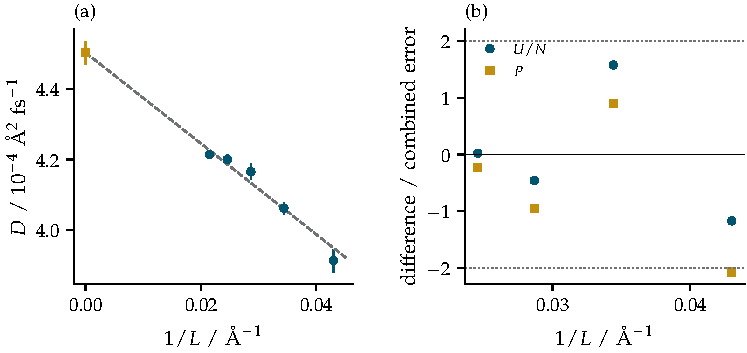
\includegraphics{ch15_convergence/size}
\caption{A result that depends on the size of the box: liquid argon at
\SI{135}{\kelvin} and $0.8\sigma^{-3}$ with 256 to 2048 atoms, two runs of
\SI{1}{\nano\second} at each size. (a) The diffusion coefficient, with its
error from blocks of \SI{100}{\pico\second}, against $1/L$, with the line
of \cref{eq:cv-yh} fitted to them (dashed) and its value at $1/L = 0$
(ochre). (b) The potential energy per atom and the pressure for each box
less those for 2048 atoms, in units of the error of the difference,
against $\pm2$ (dotted).}
\label{fig:cv-size}
\end{figure}

\begin{keyidea}
A converged average can still depend on the size of the box. The
diffusion coefficient of a periodic liquid falls short of the endless
liquid's by $2.837\kB T/(6\pi\eta_{\mathrm s}L)$, as the image flows return
through the box; runs at several sizes and a straight line in $1/L$ find
$D_\infty$. Static averages of the same liquid change far less.
\end{keyidea}

\notebook{15}{fit the line through the five boxes and extrapolate}

\begin{selfcheck}
By how much should $D$ change from a box of 500 atoms to one of 4000 at
the same density, if it follows the line of this section?
\end{selfcheck}

%=============================================================================!
% 15.8  DOES THE RUN SAMPLE ITS ENSEMBLE?                                     !
%=============================================================================!
\section{Does the run sample its ensemble?}
\label{sec:cv-ensemble}

An error bar says how well a run knows its own averages. It is silent on
whether they belong to the ensemble the run claims: Chapter~13 found
thermostats
that hold the mean temperature and get the spread of the energy wrong
(\cref{sec:th-berendsen}). This section derives a test that needs no
knowledge of the system, runs at two temperatures and the canonical
density alone\cite{Shirts2013}, and sets out the resampling that gives its
error bar.

\subsection*{The ratio of two densities}

In the canonical ensemble the probability of a microstate of energy $E$
is $\mathrm{e}^{-\beta E}/Z$ (\cref{sec:sm-canonical}). The microstates
with energies between $E$ and $E + \delta E$ number $\Omega(E)$, the
volume of that shell (\cref{sec:sm-micro}), and grouping them, as
\cref{sec:sm-kinetic} grouped the velocities by their kinetic energy,
gives the density of $E$ at the inverse temperature $\beta$, written
$\mathcal{P}(E \mid \beta)$:
\begin{equation*}
   \mathcal{P}(E \mid \beta) = \frac{\Omega(E)\,\mathrm{e}^{-\beta E}}
   {Z(\beta)\,\delta E} .
\end{equation*}
No run knows $\Omega(E)$. At two temperatures the ratio of the densities
removes it, with $\delta E$:
\begin{equation*}
   \frac{\mathcal{P}(E \mid \beta_2)}{\mathcal{P}(E \mid \beta_1)}
   = \frac{Z(\beta_1)}{Z(\beta_2)}\,\mathrm{e}^{-(\beta_2 - \beta_1)E} ,
   \qquad
   \ln\frac{\mathcal{P}(E \mid \beta_2)}{\mathcal{P}(E \mid \beta_1)}
   = \ln\frac{Z(\beta_1)}{Z(\beta_2)} + (\beta_1 - \beta_2)E .
\end{equation*}
The logarithm of the ratio of the two histograms of the energy must be a
straight line in $E$ whose slope is $\beta_1 - \beta_2$, known in advance,
whatever the system. The intercept, which holds the unknown $Z$, does not
matter. For 130 and \SI{140}{\kelvin} the slope is
\SI{6.376}{\per\electronvolt}. The test needs the two histograms to
overlap. With $C_V = 2.347\,N\kB$ for the liquid (\cref{sec:sm-kinetic}),
the mean energy rises by about $C_V\Delta T = \SI{0.518}{\electronvolt}$
(\SI{0.520}{\electronvolt} between the runs below), about twice the
canonical spread $\sqrt{\kB T^2C_V}$, \SI{0.275}{\electronvolt} at
\SI{130}{\kelvin} and \SI{0.296}{\electronvolt} at \SI{140}{\kelvin}
(\cref{eq:sm-fluctuation}), so the two share a range of energies. On
100\,000 independent energies at each temperature drawn from a gamma
density (\cref{sec:sm-kinetic}), which has the form $\Omega(E)\mathrm{e}^{-\beta
E}$ with $\Omega \propto E^{399}$, a shape chosen only so that the two
densities overlap, the fitted slope is $(6.350 \pm
0.030)$\,\si{\per\electronvolt}, its error from the bootstrap below, 0.9
errors from the required value.

\subsection*{The bootstrap}

The slope is fitted to histograms, and its error is not that of a mean.
Efron's bootstrap finds the error of any quantity computed from samples
by recomputing it on new sets, each drawn from the samples themselves
with replacement and each as large as the original set, and taking the
spread of the results\cite{Efron1979}. Drawing single samples would destroy the memory of
a run and give too small an error; drawing whole blocks, longer than the
memory, keeps it within each block, as in \cref{sec:cv-blocks}, and makes
the resampled runs nearly as correlated as the real one, losing the memory
only at the joins between blocks\cite{Kunsch1989} (\texttt{mdlab} draws
non-overlapping blocks, a simpler variant of Künsch's moving blocks). The
function \texttt{block\_bootstrap} of \texttt{mdlab.analysis.stats} does
this for several runs at once, resampling each independently. On the
\SI{2}{\nano\second} run, blocks of \SI{20}{\pico\second} give the error
of the mean potential energy as \SI{0.0045}{\electronvolt}, against
\SI{0.0047}{\electronvolt} from $g$. \Cref{sec:cv-observables} used the
same resampling for the error of a heat capacity, a variance rather than a
mean.

\subsection*{Two thermostats}

\Cref{fig:cv-ensemble} runs the liquid for \SI{1}{\nano\second} at 130 and
\SI{140}{\kelvin} under CSVR with $\tau_{\mathrm T} = \SI{1}{\pico\second}$,
and under Berendsen coupling with $\tau_{\mathrm T} = \SI{0.1}{\pico
\second}$. After the start found from each run's total energy, the mean
energies agree within 0.7 of their combined errors: $-8.6409$ and
$-8.6306$\,\si{\electronvolt} at \SI{130}{\kelvin}, $-8.1209$ and
$-8.1118$\,\si{\electronvolt} at \SI{140}{\kelvin}. The spreads do not:
0.273 and \SI{0.287}{\electronvolt} under CSVR, close to the canonical 0.275
and \SI{0.296}{\electronvolt}, and 0.112 and
\SI{0.118}{\electronvolt} under Berendsen coupling. The slope of the
logarithm of the ratio, with its error from the block bootstrap with
blocks of \SI{20}{\pico\second}, is $(6.72 \pm 0.41)$\,\si{\per\electronvolt}
under CSVR, $1.05 \pm 0.06$ times the required value and 0.8 errors from
it: CSVR passes. Under Berendsen coupling it is $(35.1 \pm
3.5)$\,\si{\per\electronvolt}, 5.5 times the required value and 8.2 errors
from it. For two Gaussian densities of the same spread $\sigma_E$ whose
means differ by $\Delta\bar E$, the logarithm of the ratio, $[(E - \bar
E_1)^2 - (E - \bar E_2)^2]/2\sigma_E^2$, is a straight line of slope
$\Delta\bar E/\sigma_E^2$. The canonical $\Delta\bar E = C_V\Delta T$ and
$\sigma_E^2 = \kB T^2C_V$ make it $\Delta T/\kB T^2 \approx \beta_1 -
\beta_2$; Berendsen coupling keeps $\Delta\bar E$ and narrows $\sigma_E$ by
a factor of 2.43, which makes the line $2.43^2 = 5.9$ times too steep, close
to the 5.5 found. A thermostat that gives the right mean and the
wrong spread fails this test at once, whatever quantity was to be
measured; the physical-validation package of Merz and Shirts carries out
this test and others for the common simulation codes\cite{Merz2018}.

\begin{figure}[htb]
\centering
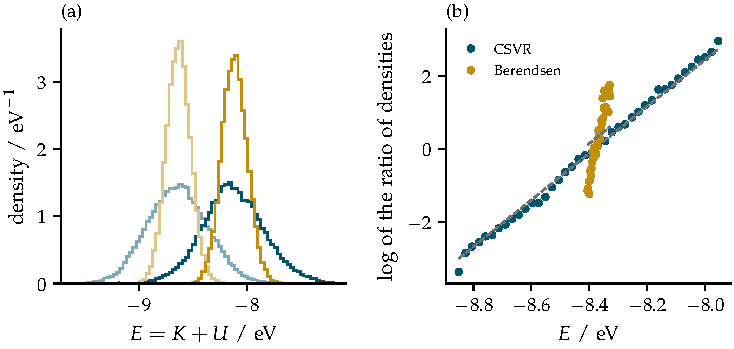
\includegraphics{ch15_convergence/ensemble}
\caption{Does the run sample its ensemble? The liquid for
\SI{1}{\nano\second} at 130 (light) and \SI{140}{\kelvin} (dark), under
CSVR (teal) and Berendsen coupling with $\tau_{\mathrm T} =
\SI{0.1}{\pico\second}$ (ochre). (a) The densities of the total energy.
(b) The logarithm of the ratio of the densities at the two temperatures,
against the slope $\beta_{130} - \beta_{140}$ that the canonical ensemble
requires (dashed).}
\label{fig:cv-ensemble}
\end{figure}

\begin{keyidea}
In the canonical ensemble $\ln[\mathcal{P}(E \mid \beta_2)/\mathcal{P}(E
\mid \beta_1)]$ is a straight line in $E$ with the slope $\beta_1 -
\beta_2$, whatever the system; runs at two nearby temperatures test it.
The error of a fitted slope, or of any quantity that is not a mean, comes
from the block bootstrap, which resamples blocks longer than the memory,
recomputes the quantity and takes the spread of the results.
\end{keyidea}

\notebook{15}{test a thermostat at two temperatures}

\begin{selfcheck}
Why does the test not need $\Omega(E)$, and what would a run at the wrong
temperature, \SI{132}{\kelvin} where \SI{130}{\kelvin} was claimed, do to
the slope?
\end{selfcheck}

%=============================================================================!
% 15.9  A PROTOCOL AND A CRITERION                                            !
%=============================================================================!
\section{A protocol and a criterion}
\label{sec:cv-protocol}

The chapter's tools combine into a procedure that takes a system from a
rough start to numbers with error bars, and a criterion, with numbers,
for when a quantity counts as converged. This section follows the liquid
from atoms placed at random to a converged run at constant pressure, with
the plot to read at each stage.

\subsection*{From random positions}

Atoms placed at random in a box overlap: 256 argon atoms dropped into the
liquid's cell start with $U = \SI{7.91e10}{\electronvolt}$ and a largest
force of \SI{2.95e12}{\electronvolt\per\angstrom}, and the first step of a
run of \SI{10}{\femto\second} would carry the atom that feels it some
\SI{4e10}{\angstrom}, across more than $10^9$ copies of the periodic box. The overlaps are
removed first by walking downhill on the energy. Moving every atom a small
distance along its own force, $\dd\vb{r}_i = h\vb{F}_i$ with $h > 0$, changes
the energy by
\begin{equation*}
   \dd U = \sum_i\grad_iU\cdot\dd\vb{r}_i = -\sum_i\vb{F}_i\cdot h\vb{F}_i
   = -h\sum_i\lvert\vb{F}_i\rvert^2 ,
\end{equation*}
which is negative unless every force vanishes: the forces point downhill,
and a step along them lowers the energy if it is short enough for the
forces not to change much along it. This is steepest descent. The function
\texttt{minimise} of \texttt{mdlab.md} sets $h$ by the atom with the
largest force, which moves the distance \texttt{step}, so that $h =
\texttt{step}/\max_i\lvert\vb{F}_i\rvert$; it keeps a trial that lowers
the energy and lengthens the next by a fifth, and refuses one that does
not and halves the distance:

\begin{code}
def minimise(
    model: EnergyForces,
    positions: ArrayLike,
    step: float = 0.1,
    force_tolerance: float = 1e-2,
    max_steps: int = 10000,
) -> tuple[NDArray, NDArray, NDArray]:
    r = np.array(positions, dtype=float)
    u, f = model(r)
    energies, largest = [u], [np.max(np.linalg.norm(f, axis=-1))]
    for _ in range(max_steps):
        if largest[-1] < force_tolerance:
            break
        trial = r + step * f / largest[-1]
        u_trial, f_trial = model(trial)
        if u_trial < u:
            r, u, f = trial, u_trial, f_trial
            energies.append(u)
            largest.append(np.max(np.linalg.norm(f, axis=-1)))
            step *= 1.2
        else:
            step *= 0.5
    return r, np.array(energies), np.array(largest)
\end{code}

\noindent From a lattice disturbed by \SI{0.2}{\angstrom} it reaches the same
minimum as ASE's FIRE optimiser, to \SI{1e-3}{\angstrom} in every position
(\texttt{test\_stats.py}). From the random start it takes 75 accepted moves
to bring the largest force below \SI{0.05}{\electronvolt\per\angstrom}, at
$U = \SI{-15.357}{\electronvolt}$ (\cref{fig:cv-protocol}(a)). The aim is
only to remove the overlaps, and any minimum close to the start will
do.

\subsection*{Temperature, then pressure}

The stages that follow each settle one thing, and each has its plot.
Velocities drawn at \SI{135}{\kelvin} for the minimised atoms give a
temperature that falls within the first picosecond to \SI{70.1}{\kelvin},
about half, as the kinetic energy shares itself with the potential energy
of atoms that sat at the bottom of their wells (\cref{sec:sm-equipartition});
CSVR brings its average over the preceding \SI{1}{\pico\second} back above
\SI{130}{\kelvin}, within \SI{5}{\kelvin} of the target, by
\SI{3.8}{\pico\second} (\cref{fig:cv-protocol}(b)), and over the last
\SI{25}{\pico\second} of \SI{50}{\pico\second} the mean is $(136.6 \pm
1.2)$\,\si{\kelvin}, 1.4 errors from the target. The running mean from the start, which lags, shows
why such a stage is discarded. Stochastic cell rescaling at
\SI{0.1}{\giga\pascal} then lets the volume move from that of
$0.8\sigma^{-3}$, \SI{12577}{\angstrom\cubed}, to the one the liquid takes
at that pressure (\cref{fig:cv-protocol}(c)), and the run continues for \SI{1}{\nano
\second}. Each quantity then goes through the criterion.

\begin{definition}
A quantity $A$, recorded at $n$ equal intervals $\dt$ over a run, is
converged to the error $\sigma^\ast$ when
\begin{enumerate}
\item the start $t_0$ that maximises $n_{\mathrm{eff}}(t_0)$ lies in the
   first half of the run (\cref{sec:cv-equilibration});
\item the $n'$ samples after it, with their own $g$ and $s$, hold at least
   100 independent samples, $n_{\mathrm{eff}} = n'/g \ge 100$
   (\cref{sec:cv-blocks});
\item the error from blocks of $5g$ samples agrees with $\sqrt{g s^2/n'}$
   within twice its own error (\cref{sec:cv-blocks});
\item the slope of the samples after $t_0$ is within two of its errors of
   zero (\cref{sec:cv-drift});
\item and $\sqrt{g s^2/n'} \le \sigma^\ast$, or else \cref{eq:cv-length}
   gives the run that would make it so (\cref{sec:cv-observables}).
\end{enumerate}
The result is reported as $\bar A \pm \sqrt{g s^2/n'}$, one standard
error, with the number of independent samples.
\end{definition}

The first check catches a run too short to locate its own start; the
second leaves at least twenty blocks of $5g$, so that the block error the
third check compares with is itself known to about a sixth,
$1/\sqrt{2\times19}$, and keeps the bias that the search for a start
brings small, as below; the third catches a slow memory that the estimate
of $g$ cut off; the fourth catches a drift or a transient left in. The
function \texttt{convergence\_report} of \texttt{mdlab.analysis.stats}
applies the first four, and the fifth when given a target, and returns
the evidence for each. The criterion says nothing about whether the run samples the
right ensemble, for which \cref{sec:cv-ensemble} gives a test, or about
the size of the box, which \cref{sec:cv-size} shows can bias a converged
number.

After \SI{300}{\pico\second} at constant pressure the report finds the
volume and the potential energy not yet converged: their starts are at
16.5 and \SI{12.0}{\pico\second}, but they hold only 64.6 and 47.8
independent samples, the potential energy now having $\tau_{\mathrm{int}}
= \SI{3.0}{\pico\second}$ over these \SI{300}{\pico\second}, as it
follows the slow swings of the volume. A
hundred independent samples need 439 and \SI{603}{\pico\second} after the
start. The pressure and the temperature pass, with 813 and 139. After
\SI{1}{\nano\second} all four pass: $V = (12310 \pm 10)$\,\si{\angstrom
\cubed} with 316 independent samples, the volume of
\cref{sec:pr-npt} within its error; $P = (0.0997 \pm 0.0004)$\,\si{\giga
\pascal} against the \SI{0.1}{\giga\pascal} asked for; $T = (135.27 \pm
0.28)$\,\si{\kelvin}; and $U = (-13.049 \pm 0.014)$\,\si{\electronvolt}.

\begin{figure}[htb]
\centering
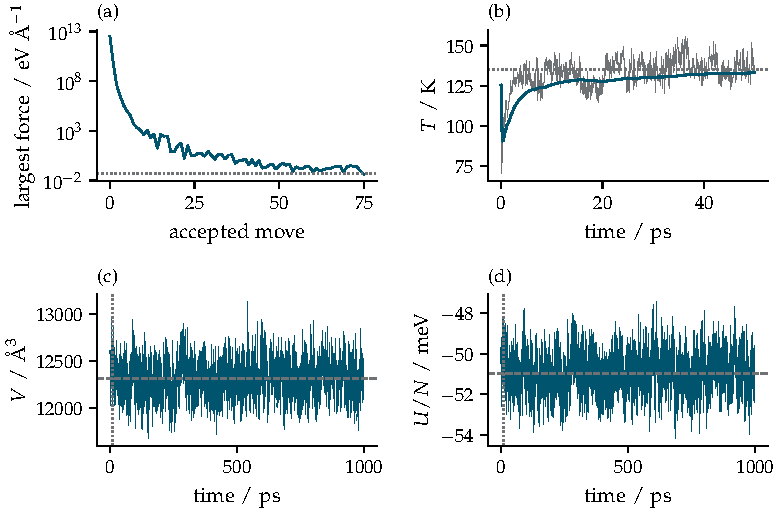
\includegraphics{ch15_convergence/protocol}
\caption{A protocol, stage by stage, for 256 argon atoms placed at random.
(a) Steepest descent: the largest force after each accepted move, against
the tolerance (dotted). (b) \SI{50}{\pico\second} of CSVR at fixed volume:
the temperature (grey) and its running mean (teal), against
\SI{135}{\kelvin} (dotted). (c) \SI{1}{\nano\second} of stochastic cell
rescaling at \SI{0.1}{\giga\pascal}: the volume, the start found (dotted)
and the mean after it (dashed). (d) The same for the potential energy per
atom.}
\label{fig:cv-protocol}
\end{figure}

\subsection*{Does the criterion keep its promise?}

An error bar of one standard error should hold the true mean in 68\% of
runs. On series of known mean from \cref{eq:cv-ou}, 300 of each length,
the error bar the report gives, whether or not the series passes, holds it
in 0.55 of the series with 25
independent samples, 0.57 with 50, 0.68 with 100 and 0.70 with 200; the
error bar $\sqrt{g s^2/n}$ of the whole series, without the search for a
start, holds it in 0.64, 0.64, 0.71 and 0.72. The search favours a start
after which $g$ happens to come out small (\cref{sec:cv-equilibration}),
which makes the error bar small too, and only with about a hundred
independent samples does that bias fade, which sets the threshold of the
second check. With the offset of \cref{fig:cv-equilibration}(a) added to
series of \SI{200}{\pico\second}, 182 of 200 pass the criterion, and of
those 0.70 hold the true mean within one error and 0.95 within two. On the
liquid itself the evidence is thinner: of the sixty pieces of
\SI{100}{\pico\second} of $U$, $T$ and $P$ in the \SI{2}{\nano\second} run,
ten pass, and of those four hold the mean of the whole run within one
error and seven within two, fewer than 68\% and 95\% would give, which
fits pieces that pass only where $g$ came out small.

\begin{keyidea}
A protocol removes overlaps by steepest descent, brings the temperature,
then the pressure, to their targets, and discards each stage. A quantity
is converged when its start lies in the first half of the run, at least
100 independent samples follow it, blocks confirm the error, no drift
remains and the error meets its target; \texttt{convergence\_report} checks
all five. So reported, one error bar holds the true mean of test series in
about 68\% of runs; on the liquid's pieces that only just pass, less
often.
\end{keyidea}

\notebook{15}{run the criterion on any series, from mdlab or from ASE}

\begin{selfcheck}
A run of \SI{500}{\pico\second} has $g = 300$ for a quantity sampled every
\SI{10}{\femto\second}. Does it pass the second check, and if not, how long
must it be?
\end{selfcheck}

%=============================================================================!
% 15.10  WHAT THE TRAJECTORY LOOKS LIKE                                       !
%=============================================================================!
\section{What the trajectory looks like}
\label{sec:cv-trajectory}

Each fault of this chapter lies in the numbers drawn from a trajectory,
and each shows on one of four plots of the quantity concerned, which
together we call its dashboard: the series with the start found, the
running mean from that start with its error band, the errors from blocks,
and the autocorrelation function. This section shows the dashboard of a
healthy run, then six runs or analyses that go wrong, each with the check
that catches it.

\subsection*{A healthy run}

\Cref{fig:cv-healthy} is the dashboard of the volume in the
\SI{1}{\nano\second} at constant pressure that ends the protocol of
\cref{sec:cv-protocol}, drawn by \texttt{dashboard} of the chapter's
scripts. (a) The series has settled by the start found at
\SI{10}{\pico\second} and then wanders about its mean with no trend. (b)
The running mean from the start swings while few independent samples are
in it and then holds steady inside its error band, which narrows as one
over the square root of the time since the start. (c) The error from
blocks rises to a plateau, 9.6 with its own error of 1 against
\SI{9.8}{\angstrom\cubed} from $g$. (d) The autocorrelation function falls
to zero by \SI{8}{\pico\second}, where the estimate of $g$ stops. The
report, given no target, passes all four checks: $V = (12310.4
\pm 9.8)$\,\si{\angstrom\cubed} from 316 independent samples, with a slope
0.85 of its error.

\begin{figure}[htb]
\centering
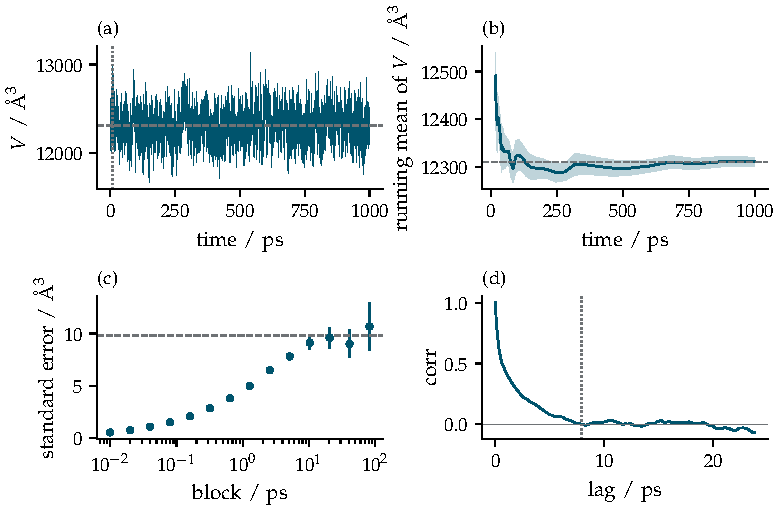
\includegraphics{ch15_convergence/healthy}
\caption{The dashboard of a converged quantity: the volume over
\SI{1}{\nano\second} at \SI{0.1}{\giga\pascal}. (a) The series, the start
found (dotted) and the mean after it (dashed). (b) The running mean from
the start with its error band. (c) The error of the mean from blocks,
against $\sqrt{g s^2/n}$ (dashed). (d) The autocorrelation function, with
the lag at which the estimate of $g$ stops (dotted).}
\label{fig:cv-healthy}
\end{figure}

\subsection*{Six faults}

\Cref{fig:cv-faults} and \cref{tab:cv-faults} set six faults against
healthy runs.

\begin{table}[htb]
\centering
\small
\caption{The faults of \cref{fig:cv-faults}, the check that catches each,
and its value in the healthy and the faulty run or analysis.}
\label{tab:cv-faults}
\begin{tabular}{@{}>{\raggedright\arraybackslash}p{0.22\linewidth}
   >{\raggedright\arraybackslash}p{0.27\linewidth}
   >{\raggedright\arraybackslash}p{0.21\linewidth}
   >{\raggedright\arraybackslash}p{0.21\linewidth}@{}}
\toprule
fault & check & healthy & faulty\\
\midrule
(a) averaged from the start & the start found; the mean after it &
start \SI{2.8}{\pico\second}, $\bar U/N = (-50.060 \pm
0.085)$\,\si{\milli\electronvolt} &
$\bar U/N = \SI{-50.173}{\milli\electronvolt}$ from $t = 0$\\
(b) the naive error bar & pieces whose bars hold the mean of
\SI{2}{\nano\second} & 11 of 20 with $\sqrt g$ & 0 of 20 with $s/\sqrt
n$\\
(c) too short for a plateau & independent samples; the blocks &
1369 in \SI{2}{\nano\second} & 19.7 in \SI{20}{\pico\second}, no
plateau\\
(d) a drifting energy & the drift test & $-0.9$ errors at
\SI{10}{\femto\second} & $+9.3$ errors at \SI{35}{\femto\second}\\
(e) the wrong ensemble & slope of the ratio of densities, over the
required & $1.05 \pm 0.06$ (CSVR) & $5.50 \pm 0.55$ (Berendsen)\\
(f) a box too small & $\ens{\Delta r^2}/6t$ at \SI{20}{\pico\second}, in
\SI{e-4}{\angstrom\squared\per\femto\second} &
4.177 for 2048 atoms & 3.863 for 256\\
\bottomrule
\end{tabular}
\end{table}

\emph{(a) Averaged from the start.} A run started on the lattice and
averaged from its first step includes the melting: the mean of $U/N$ over
the \SI{100}{\pico\second} is \SI{-50.173}{\milli\electronvolt}, while from
the start found at \SI{2.8}{\pico\second} it is $(-50.060 \pm
0.085)$\,\si{\milli\electronvolt}, against \SI{-50.092}{\milli\electronvolt}
over \SI{2}{\nano\second}. The running mean from $t = 0$ in
\cref{fig:cv-faults}(a) creeps up for the whole run, the offset fading
only as one over the length of the run. In this run the shift is about one
error bar; over the eight runs of \cref{sec:cv-equilibration} the discard
moves the mean by \SI{0.106}{\milli\electronvolt}, 1.6 of their
error bars. Even the \SI{2}{\nano\second} run, started from an
equilibrated liquid, has its start found at \SI{30}{\pico\second}: the
search costs little where there is nothing to discard.

\emph{(b) The naive error bar.} $s/\sqrt n$ treats the 10\,000 samples of
a piece of \SI{100}{\pico\second} as independent. Its bars are too short
by the factor $\sqrt g$, about twelve, and none of the twenty holds the
mean of the whole run, where the bars with $\sqrt g$ hold it in eleven,
against the fourteen that 68\% would give, within the spread of two that
twenty pieces allow (\cref{fig:cv-faults}(b)). The check is to report $g$ with every error
bar.

\emph{(c) Too short for a plateau.} The first \SI{20}{\pico\second} of the
run hold 19.7 independent samples of $U$. Its block errors rise without
levelling (\cref{fig:cv-faults}(c)), and its start falls in the second
half of the run, at \SI{12}{\pico\second}: the report fails it on the start
and on 100 independent samples. Its block check passes, because the
\SI{8}{\pico\second} after that start give $g = 13$, a tenth of the value
of the whole run, and blocks of $5g$ that short agree with an error as
short; the plot of the blocks shows what the check cannot.

\emph{(d) A drifting energy.} With steps of \SI{35}{\femto\second} the
total energy of a run at fixed energy climbs by
\SI{0.6}{\milli\electronvolt} per atom in a nanosecond
(\cref{fig:cv-faults}(d)), 9.3 errors of the drift test, and moves the
temperature by \SI{3.2}{\kelvin} per nanosecond; with steps of
\SI{10}{\femto\second} its slope is $-0.9$ errors, no drift.

\emph{(e) The wrong ensemble.} Berendsen coupling with $\tau_{\mathrm T} =
\SI{0.1}{\pico\second}$ gives the right mean energies and the wrong
spread, and the logarithm of the ratio of its energy densities at 130 and
\SI{140}{\kelvin} rises 5.5 times too steeply (\cref{fig:cv-faults}(e)).
None of the convergence checks finds this, since each run is converged in
its own narrow ensemble; the test of \cref{sec:cv-ensemble} does, as does
the spread of $K$ set against the canonical one (\cref{sec:th-compare}).

\emph{(f) A box too small.} The squared displacement over $6t$, whose
value at long times is $D$, reaches \SI{3.863e-4}{\angstrom\squared\per
\femto\second} at \SI{20}{\pico\second} for 256 atoms and $4.177\times
10^{-4}$ for 2048, so the smaller box gives 0.925 times the larger's
(\cref{fig:cv-faults}(f)); these are single runs read at one time, near
the 3.914 and 4.214 of \cref{sec:cv-size}. Each run fixes its own $D$
to about 1\%; the smaller box fixes it at a different number, for the
reason \cref{sec:cv-size} gives.

\begin{figure}[htb]
\centering
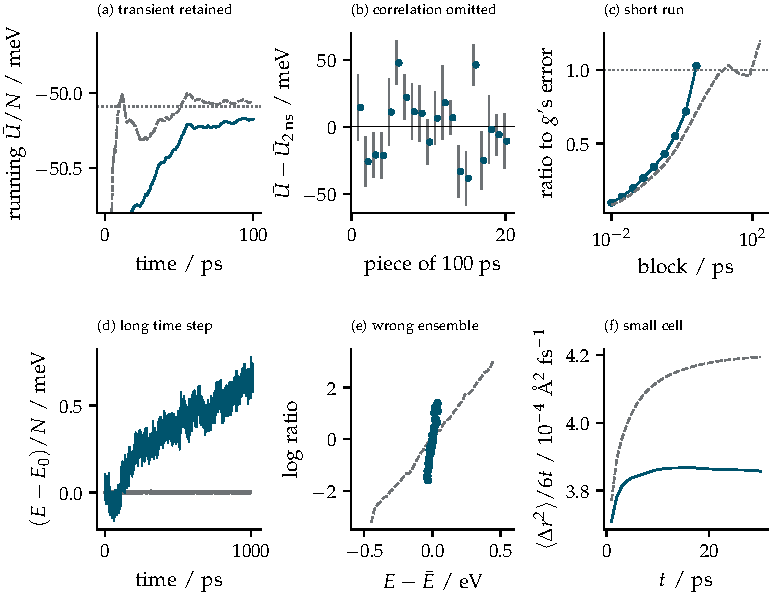
\includegraphics{ch15_convergence/faults}
\caption{Faults of convergence (teal) against healthy runs (grey dashed).
(a) The running mean of $U/N$ of a melting run from $t = 0$, against that
from the start found, and the mean of \SI{2}{\nano\second} (dotted). (b)
Twenty pieces of \SI{100}{\pico\second}: the mean of $U$ less that of the
whole run, with $s/\sqrt n$ (teal, too short to see) and $\sqrt{g s^2/n}$
(grey). (c) The error of $U$ from blocks over the first
\SI{20}{\pico\second} and over \SI{2}{\nano\second}, each over its
$\sqrt{g s^2/n}$. (d) The total energy per atom at fixed energy at 35 and
\SI{10}{\femto\second}. (e) The logarithm of the ratio of the energy
densities at 140 and \SI{130}{\kelvin} under Berendsen coupling (here in
teal, as the fault) and CSVR, each about its mean. (f) The squared displacement over $6t$ for 256 and
2048 atoms.}
\label{fig:cv-faults}
\end{figure}

\begin{practice}
A run is read through the dashboard of each quantity to be reported: the
series with its start, the running mean with its error band, the block
errors with their plateau, and the autocorrelation function. Every average
is reported with its error bar, its number of independent samples and the
start discarded, and passes \texttt{convergence\_report}; a run that fails
is extended by the length \cref{eq:cv-length} gives. A thermostat is
checked once by the test of \cref{sec:cv-ensemble}, a time step by the
drift test at fixed energy, and a transport coefficient by a second box
size.
\end{practice}

\begin{keyidea}
Each fault of convergence shows on a plot of the dashboard or on one of the
chapter's tests: the start for an average taken from the first step, $g$ for
a naive error bar, the block plateau for a run too short, the drift test
for a creeping energy, the ratio of densities for a thermostat that
narrows the spread, and a second box for a size-dependent result.
\end{keyidea}

\notebook{15}{break each run in turn and watch which check catches it}

\begin{selfcheck}
A paper reports $D$ from one run of 256 argon atoms as $(3.87 \pm 0.04)
\times10^{-4}$\,\si{\angstrom\squared\per\femto\second}. Is the error bar
the error of $D$?
\end{selfcheck}

%=============================================================================!
% 15.S  WHAT WE NOW HAVE                                                      !
%=============================================================================!
\unnumbered{What we now have}

The mean of $n$ independent samples spreads by $\sigma_x/\sqrt n$, and its
error is estimated as $s/\sqrt n$; the samples of a run remember their
predecessors, and $n$ of them are worth $n/g$ independent ones, with the
statistical inefficiency $g = 1 + 2\sum_k\operatorname{corr}(k)$ estimated
by summing the autocorrelation function until it first reaches zero, or a
run of length $t_{\mathrm f}$ worth $t_{\mathrm f}/(2\tau_{\mathrm{int}})$.

Block averages give the same error without the autocorrelation function
and show by their plateau
whether the run was long enough to know it. The start of a run is found as
the one that leaves the most independent samples, a drift as the slope of
a straight line with its correlated error, and the run a precision needs
from $t_{\mathrm f} \ge 2\tau_{\mathrm{int}}\sigma_A^2/\sigma^{\ast2}$.
For liquid argon
under CSVR the energy-like quantities have $\tau_{\mathrm{int}}$ of about
\SI{1}{\pico\second}, ten times longer than at fixed energy, because the
thermostat moves the energy slowly. With these error bars the diffusion
coefficient is the same under CSVR with $\tau_{\mathrm T} =
\SI{1}{\pico\second}$, Berendsen coupling with $\tau_{\mathrm T} =
\SI{0.1}{\pico\second}$ and fixed energy to about 2\%, but depends on the
size of the box as $1/L$, by 13\% for 256 atoms.
The ratio of the energy densities at two temperatures tests whether
a thermostat samples the canonical ensemble: CSVR passes, Berendsen
coupling fails by a factor of 5.5. A protocol takes atoms from random
positions by steepest descent, a thermostat and a barostat to a run whose
quantities pass a five-point criterion, under which one error bar holds
the true mean of test series in about 68\% of runs.

Chapter~16 defines the observables that describe a liquid's structure and
motion, among them the radial distribution function, the mean squared
displacement and the viscosity that \cref{sec:cv-size} inferred, and
reports each with the error bar and the criterion of this chapter.

%=============================================================================!
% 15.A  ANSWERS TO THE CHECKS                                                 !
%=============================================================================!
\unnumbered{Answers to the checks}
\label{sec:cv-answers}

\answerto{sec:cv-mean}The error falls as $1/\sqrt n$, so a fifth of it
needs $5^2 = 25$ times as many samples: 2500.

\answerto{sec:cv-correlation}$g = (1 + 0.5)/(1 - 0.5) = 3$, and 1000
samples are worth $1000/3 = 333$ independent ones.

\answerto{sec:cv-blocks}Blocks of $5g = 500$ samples miss about 5\% of
the error, and the run holds $20\,000/500 = 40$ of them, which give the
error to $1/\sqrt{2\times39} = 0.11$.

\answerto{sec:cv-equilibration}About $\delta A_0\,\tau_{\mathrm r}/t_{\mathrm f} = 2\times
1/100 = \SI{0.02}{\kelvin}$.

\answerto{sec:cv-drift}It is 1.5 errors from zero, so the run shows no drift
it can detect. A run four times as long has an error $4^{3/2} = 8$ times
smaller, 0.25, and if the true slope is 3 the longer run would put it 12
errors from zero: a drift.

\answerto{sec:cv-observables}$t_{\mathrm f} \ge 2\times\SI{5}{\pico\second}\times2^2/
0.1^2 = \SI{4000}{\pico\second}$, \SI{4}{\nano\second}.

\answerto{sec:cv-size}At the same density $L$ grows as $N^{1/3}$, so $L$
doubles from \SI{29.07}{\angstrom} to \SI{58.14}{\angstrom}, and $D$ rises
by $12.88\times(1/29.07 - 1/58.14) = 0.221$ in units of
\SI{e-4}{\angstrom\squared\per\femto\second}.

\answerto{sec:cv-ensemble}$\Omega(E)$ is the same at both temperatures and
cancels in the ratio. A run at \SI{132}{\kelvin} labelled \SI{130}{\kelvin}
has the slope $\beta_{132} - \beta_{140} = \SI{5.024}{\per\electronvolt}$,
0.79 of the $\SI{6.376}{\per\electronvolt}$ required, which an error of
about 0.4 shows as some three errors.

\answerto{sec:cv-protocol}The run holds $50\,000/300 = 167$ independent
samples, so it passes the second check, provided the start found leaves at
least $100\times300 = 30\,000$ samples after it.

\answerto{sec:cv-trajectory}No. The bar is the statistical error of $D$ in
that box. A box of 256 atoms gives a $D$ some 13\% below that of an
infinite one (\cref{sec:cv-size}), a bias many times larger than the bar,
which the error bar of a single box cannot show.

%=============================================================================!
% 15.E  EXERCISES                                                             !
%=============================================================================!
\unnumbered{Exercises}
\label{sec:cv-exercises}

The exercises run from questions of understanding, through calculations,
to short derivations marked `show that'. Full solutions are in
\hyperref[sec:cv-solutions]{`Solutions to the exercises'} at the end of
the book, and Notebook~15 checks every numerical answer.

\begin{exercise}[enough rolls]
\label{ex:cv-rolls}
How many rolls of a fair die make the interval $\bar x \pm 1.96\,\sigma_{\bar
x}$ no wider than $\pm0.01$?
\end{exercise}

\begin{exercise}[five samples]
\label{ex:cv-student}
With five samples, Student's 95\% factor is 2.776. By what fraction is the
95\% interval wider than one built with 1.96, and why must it be?
\end{exercise}

\begin{exercise}[the variance of a difference]
\label{ex:cv-cov}
Show that $\operatorname{var}(x - y) = \operatorname{var}(x) +
\operatorname{var}(y) - 2\operatorname{cov}(x, y)$, and explain why
\cref{sec:cv-observables} took the difference of the two species'
temperatures at each frame as one series, rather than combining the errors
of the two temperatures.
\end{exercise}

\begin{exercise}[a series that settles]
\label{ex:cv-ou-var}
Show that the step of \cref{eq:cv-ou}, started from $x_0 = 0$, gives
$\operatorname{var}(x_k) = 1 - c^{2k}$, and find how many steps of $c =
0.95$ bring the variance within 1\% of 1.
\end{exercise}

\begin{exercise}[a slower memory]
\label{ex:cv-g-ou}
For the step of \cref{eq:cv-ou} with $c = 0.99$ and samples
\SI{10}{\femto\second} apart, find $g$, $\tau_{\mathrm{int}}$ and
$\tau_{\mathrm c}$, and the number of independent samples in a run of
\SI{1}{\nano\second}.
\end{exercise}

\begin{exercise}[a weighted geometric sum]
\label{ex:cv-ksum}
Show that $\sum_{k=1}^\infty kc^k = c/(1 - c)^2$ for $0 \le c < 1$, by
multiplying the sum by $1 - c$.
\end{exercise}

\begin{exercise}[the error of an error]
\label{ex:cv-error-error}
For $n$ independent Gaussian samples $u_i$ of mean zero and variance
$\sigma_u^2$, show that $\ens{u^4} = 3\sigma_u^4$, and hence that $s'^2 =
\frac1n\sum_iu_i^2$ has the variance $2\sigma_u^4/n$, so that $s'$ has the
relative error $1/\sqrt{2n}$.
\end{exercise}

\begin{exercise}[blocks long enough]
\label{ex:cv-block-length}
A run of $2^{16}$ samples has $g = 60$ and an exponential memory. How long
must its blocks be to miss about 5\% of the error, how many such blocks does it hold, and how
precisely does their spread give the error?
\end{exercise}

\begin{exercise}[what a transient leaves]
\label{ex:cv-offset}
A run of length $t_{\mathrm f}$ carries the offset $\delta A_0\,\mathrm{e}^{-t/\tau_{\mathrm
r}}$. Show that after discarding the first $t_0$, the offset adds
$\delta A_0\,\tau_{\mathrm r}(\mathrm{e}^{-t_0/\tau_{\mathrm r}} -
\mathrm{e}^{-t_{\mathrm f}/\tau_{\mathrm r}})/(t_{\mathrm f} - t_0)$ to the mean, and evaluate it for
$\delta A_0 = 3$, $\tau_{\mathrm r} = \SI{2}{\pico\second}$, $t_{\mathrm f} =
\SI{50}{\pico\second}$ and $t_0 = \SI{5.34}{\pico\second}$.
\end{exercise}

\begin{exercise}[evenly spaced times]
\label{ex:cv-stt}
Show that for $n$ times $t_i = i\dt$, $i = 1, \dots, n$,
$\sum_i(t_i - \bar t)^2 = n(n^2 - 1)\dt^2/12$, using $\sum_ii^2 = n(n +
1)(2n + 1)/6$.
\end{exercise}

\begin{exercise}[a longer run, a smaller drift]
\label{ex:cv-drift-limit}
The largest harmless drift for a run of \SI{1}{\nano\second} at fixed
energy is \SI{20.8}{\micro\electronvolt} per atom per nanosecond. Show
that the limit falls as $t_{\mathrm f}^{-3/2}$ with the run's length $t_{\mathrm f}$, and evaluate it
for \SI{10}{\nano\second}.
\end{exercise}

\begin{exercise}[too long a step]
\label{ex:cv-steepest}
For $U = \frac12kx^2$ in one dimension, show that a step of steepest
descent, $x \to x + hF$, lowers $U$ only if $0 < h < 2/k$, and that $h =
1/k$ reaches the minimum in one step.
\end{exercise}

\begin{exercise}[the pressure to a precision]
\label{ex:cv-pressure}
How long a run under CSVR, with the spread and $\tau_{\mathrm{int}}$ of
\cref{tab:cv-observables}, fixes the pressure of the liquid to
$\pm\SI{0.0005}{\giga\pascal}$? And at fixed energy, where a sample of the
pressure spreads by \SI{0.0096}{\giga\pascal}?
\end{exercise}

\begin{exercise}[a run too short]
\label{ex:cv-short}
A quantity with $\tau_{\mathrm{int}} = \SI{2}{\pico\second}$ is recorded in
a run of \SI{150}{\pico\second}, whose start is found at
\SI{10}{\pico\second}. Does it pass the second check of the criterion, and
if not, how much longer must the run be?
\end{exercise}

\begin{exercise}[the ratio for a gamma density]
\label{ex:cv-gamma-ratio}
Show that for $\mathcal{P}(E \mid \beta) \propto E^{a-1}\mathrm{e}^{-\beta E}$
the logarithm of the ratio of the densities at $\beta_2$ and $\beta_1$ is
a straight line in $E$ with the slope $\beta_1 - \beta_2$, and find the
slope for 300 and \SI{310}{\kelvin}.
\end{exercise}

\begin{exercise}[the units of the correction]
\label{ex:cv-units}
Show that $\kB T/(\eta_{\mathrm s}L)$ has the units of a diffusion
coefficient, and that no other product of powers of $\kB T$,
$\eta_{\mathrm s}$ and $L$ does.
\end{exercise}

\begin{exercise}[the size of the correction]
\label{ex:cv-yh}
With $\eta_{\mathrm s} = \SI{2.18e-4}{\pascal\second}$, find the
Yeh-Hummer correction $2.837\kB T/(6\pi\eta_{\mathrm s}L)$ for the liquid of
256 atoms, $L = \SI{23.26}{\angstrom}$, at \SI{135}{\kelvin}, in
\si{\angstrom\squared\per\femto\second}.
\end{exercise}

\begin{exercise}[why blocks]
\label{ex:cv-why-blocks}
Why does a bootstrap that draws single samples from a run, rather than
blocks, give too small an error, and how long must the blocks be?
\end{exercise}

\begin{exercise}[a referee's question]
\label{ex:cv-referee}
A study reports the heat capacity of a liquid from one run of
\SI{50}{\pico\second} at fixed energy as $2.29\,N\kB$, `converged, since
the running mean of $K$ is flat'. What has it not shown, and what would
show it?
\end{exercise}


%=============================================================================!
% CHAPTER 16  OBSERVABLES                                                     !
%=============================================================================!
\chapter{Observables}
\label{ch:observables}

%=============================================================================!
% 16.0  CHAPTER OPENING                                                       !
%=============================================================================!
A trajectory records positions and velocities. To learn from it, we
need to turn those records into quantities that answer physical
questions: how the atoms are arranged, how far they move, or how often
they react. Such an observable may be a single number or a whole curve.
It also gives us something to compare between simulations, and, where
the measurement corresponds, with experiment.

We begin with structure: the distribution of neighbours, the structure
factor measured by diffraction, and the bonds that identify molecules
and reactions. Displacements and velocity correlations then give two
routes to diffusion, followed by the transport of charge and momentum.
The Fourier transform separates vibrations by frequency. Finally,
histograms of selected coordinates give free-energy profiles.

The error estimates of Chapter~15 accompany these measurements. Identities
between observables and comparisons with independent implementations
provide checks on the analysis. The same quantities will later be used
to judge learned models of motion against their reference trajectories
in the planned Part~VI.

%=============================================================================!
% 16.1  HOW ATOMS ARRANGE THEMSELVES                                          !
%=============================================================================!
\section{How atoms arrange themselves}
\label{sec:ob-rdf}

An orchard and a wood can hold the same number of trees on the same area
and still look different. Standing at one tree of an orchard planted on a
square grid, a walker finds the nearest trees at one spacing, the next at
$\sqrt2$ spacings, then at 2, each at a fixed distance and in a fixed
number. In a wood no two trees grow closer than their trunks allow, the
nearest neighbours lie at roughly one distance without fixed directions,
and farther out the trees thin into an even scatter. Counting the trees in
rings of equal width around one tree, and comparing each count with what
an even scatter would give, tells the two apart without a map. Atoms in a
crystal and in a liquid differ in the same way, and the count in rings is
the radial distribution function.

\subsection*{The radial distribution function}

Around an atom, the number of others whose centres lie between the
distances $r$ and $r + \dd r$ would be the number density $\rho = N/V$
times the volume of that thin shell, $4\pi r^2\,\dd r$, if the atoms were
scattered evenly and independently. The radial distribution function
$g(r)$ is the factor by which the actual mean number differs:
\begin{equation}
   \text{mean number of partners between $r$ and $r + \dd r$}
   = \rho\,g(r)\,4\pi r^2\,\dd r .
   \label{eq:ob-rdf}
\end{equation}
Where $g(r) > 1$ partners crowd; where $g(r) < 1$ they are scarce; and
$g(r) = 0$ inside the distance at which two atoms repel too strongly to
meet. The mean is over every atom as the centre and over every frame of
the run, so $g(r)$ describes the whole liquid or crystal.
Summing \cref{eq:ob-rdf} out to a distance $r$ counts the partners within
$r$ of an atom, the running coordination number
\begin{equation*}
   n_{\mathrm c}(r) = \rho\int_0^r g(s)\,4\pi s^2\,\dd s ,
\end{equation*}
whose value at the end of the first shell of neighbours is the atom's
number of nearest neighbours.

A run gives $g(r)$ as a histogram (\cref{sec:sm-probability}). The
distances are cut into bins of width $\delta r$; in each frame, every pair
closer than the last edge adds one to its bin for each of its two atoms,
since each is the other's partner; and the total over $n$ frames is
divided by the count an even scatter would give, $nN\rho$ times the volume
of the shell between the edges $r_k$ and $r_{k+1}$,
\begin{equation*}
   \tfrac43\pi\bigl(r_{k+1}^3 - r_k^3\bigr)
   = 4\pi r_k^2\,\delta r + 4\pi r_k\,\delta r^2
   + \tfrac43\pi\,\delta r^3 ,
\end{equation*}
by expanding the cube of $r_k + \delta r$. The exact difference of
spheres is used rather than its first term $4\pi r_k^2\,\delta r$, which
misses the shell's volume by a fraction of about $\delta r/r_k$, large near
the origin and the whole of it in the first bin, where $r_k = 0$. In a
periodic cell the separations are reduced to their nearest image
(\cref{sec:md-image}). That finds every pair once only out to half the
cell's smallest width; beyond it a sphere around an atom would hold more
than one copy of some partners while the nearest image counts one, so the
histogram stops there. A partial function $g_{\mathrm{AB}}(r)$, the
partners of kind B around atoms of kind A, takes A atoms as the centres,
B atoms as the partners and $\rho_{\mathrm B} = N_{\mathrm B}/V$ as the
density.

The function \texttt{rdf} of \texttt{mdlab.analysis.structure} does this,
finding the pairs through the cell list of \cref{sec:md-neighbours}:

\begin{code}
def rdf(
    positions: ArrayLike,
    cell: ArrayLike,
    r_max: float,
    n_bins: int,
    centres: ArrayLike | None = None,
    partners: ArrayLike | None = None,
    per_frame: bool = False,
) -> tuple[NDArray, NDArray]:
    frames = _frames(positions)
    h = np.asarray(cell, dtype=float)
    in_a = _chosen(frames.shape[1], centres)
    in_b = _chosen(frames.shape[1], partners)
    edges = np.linspace(0.0, r_max, n_bins + 1)
    ideal = in_a.sum() * in_b.sum() / cell_volume(h) * shell_volumes(edges)
    out = np.empty((len(frames), n_bins))
    for k, r in enumerate(frames):
        i, j, _, dist = cell_list_pairs(r, h, r_max)
        # a pair counts once for each end that is a centre whose partner
        # is the other end
        weight = (in_a[i] & in_b[j]).astype(float) + (in_a[j] & in_b[i])
        out[k] = np.histogram(dist, edges, weights=weight)[0] / ideal
    middle = 0.5 * (edges[1:] + edges[:-1])
    return middle, (out if per_frame else out.mean(axis=0))
\end{code}

\noindent It divides by $N\rho = N^2/V$, as ASE's \texttt{get\_rdf}
does\cite{Larsen2017}, and agrees with it to \num{3e-14} on 50 frames of
liquid argon. One consequence of that choice shows far from any atom.
For atoms placed independently at random, an atom's partners are the
other $N - 1$, spread evenly over the volume $V$, while the divisor
assumes $N$, so $g(r)$ tends to $(N - 1)/N = 1 - 1/N$. For 256 atoms
placed at random in the liquid's cell, 400 times over, $g(r)$ averages
$0.9961 \pm 0.0005$ beyond \SI{2}{\angstrom}, against $1 - 1/256 = 0.9961$
(\cref{fig:ob-rdf}a). A liquid falls short of 1 by less. Each atom clears
a hole around itself that holds fewer partners than an even scatter, and
\cref{sec:ob-sq} shows that the hole takes $1 - S(0)$ of the one partner
missing from $\rho V$, with $S(0)$ about 0.06 here, leaving only $S(0)$
missing from the rest of the cell; $g(r)$ then tends to $1 - S(0)/N$, once
the cell is large enough for the liquid's order to die away within it.
Beyond the sphere of radius $L/2$, in the corners of the 2048-atom cell
of Chapter~15, the partners lie at $0.999967 \pm 0.000005$ of $\rho$,
against $1 - 1/2048 = 0.999512$. In the 256-atom cell, where $g(r)$ still
ripples by a few hundredths at $L/2$, no far value is reached.

\subsection*{A crystal and a liquid}

The fcc crystal of the model argon of Chapters~10 to 15, at its own
lattice constant of \SI{5.26714}{\angstrom} and \SI{21}{\kelvin}, has
$g(r)$ in sharp peaks at the distances of its shells of neighbours,
$(a/\sqrt2)\sqrt m$, for $m = 1$ to 5: \num{3.724}, \num{5.267},
\num{6.451}, \num{7.449} and \SI{8.328}{\angstrom}
(\cref{fig:ob-rdf}b). Between the peaks $g(r)$ is zero, and $n_{\mathrm c}(r)$
climbs in steps of 12, 6, 24 and 12, the numbers of atoms in the first
four shells of the fcc lattice, to 12, 18, 42 and 54 at the gaps between
them (\cref{fig:ob-rdf}c). The peaks have width because the atoms vibrate,
each wandering from its mean position by \SI{0.094}{\angstrom} along each
axis (root mean square), and the first rises to 9.30.

The liquid at \SI{135}{\kelvin} and $\rho = \SI{0.02035}{\per\angstrom
\cubed}$ (Chapter~15's run of \SI{2}{\nano\second}, every
\SI{2}{\pico\second}) has none of this order beyond a few neighbours.
$g(r)$ is zero inside \SI{3}{\angstrom}, rises to a first peak of 2.578 at
\SI{3.684}{\angstrom}, falls to a first minimum of 0.663 at
\SI{5.238}{\angstrom}, and then oscillates about 1 with peaks that weaken
shell by shell. Out to its first minimum the liquid holds 12.00
neighbours on average, as many as the crystal's first shell, though
spread over a wider range of distances, at no fixed directions, and at a
density of \SI{0.02035}{\per\angstrom\cubed} against the crystal's
\SI{0.02737}{\per\angstrom\cubed}.

\begin{figure}[htb]
\centering
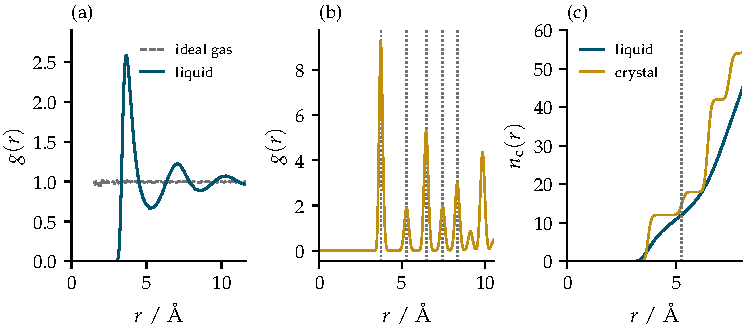
\includegraphics{ch16_observables/rdf}
\caption{(a) The radial distribution function of liquid argon at
\SI{135}{\kelvin} (Chapter~15's run of \SI{2}{\nano\second}, every
\SI{2}{\pico\second}) against 256 atoms at random in the same cell
(dashed, from \SI{1.5}{\angstrom}, where its bins hold enough pairs).
(b) The fcc crystal at \SI{21}{\kelvin}, with the distances of its first
five shells (dotted). (c) The running coordination number of the liquid
and the crystal, with the liquid's first minimum (dotted).}
\label{fig:ob-rdf}
\end{figure}

\subsection*{Energy and pressure from the arrangement}

For a pair potential, $g(r)$ holds all that the potential energy and the
virial need. The potential energy is the sum of $\varphi(r_{ij})$ over pairs.
Around one atom, \cref{eq:ob-rdf} puts $\rho g(r)4\pi r^2\dd r$ partners
at the distance $r$, each contributing $\varphi(r)$; summing over the $N$
atoms counts each pair from both ends, so
\begin{equation*}
   \ens{U} = \frac N2\,\rho\int_0^\infty\varphi(r)\,g(r)\,4\pi r^2\,\dd r .
\end{equation*}
The virial of \cref{sec:pr-periodic}, $\mathcal{W} = -\sum_{\text{pairs}}
r_{ij}\varphi'(r_{ij})$, follows by the same count,
\begin{equation*}
   \ens{\mathcal{W}} = -\frac N2\,\rho\int_0^\infty r\varphi'(r)\,g(r)\,
   4\pi r^2\,\dd r ,
\end{equation*}
and with it and the run's mean kinetic energy the pressure $\ens{P} =
(2\ens{K} + \ens{\mathcal{W}})/3V$ of \cref{eq:pr-virial}. On bins of
\SI{0.01}{\angstrom} and the 1000 frames, these give $U/N =
\SI{-50.102}{\milli\electronvolt}$ against the run's average of $(-50.092
\pm 0.018)$\,\si{\milli\electronvolt}, 0.6 errors away, and $P =
\SI{0.0848}{\giga\pascal}$ against $(0.0849 \pm 0.0004)$\,\si{\giga
\pascal}, 0.2 errors away. The bins must be fine: on bins of
\SI{0.05}{\angstrom} the energy misses by 1.9 errors, because $\varphi$
changes steeply across a bin near the core. Agreement here is a check of
the normalisation of $g(r)$, of its histogram and of the run's energy
together.

\subsection*{How long the arrangement takes}

Chapter~15 deferred the convergence of $g(r)$ to this chapter. One frame
already averages over 256 centres, so in bins of \SI{0.05}{\angstrom} its
$g(r)$ at the first peak spreads by only 0.33 from frame to frame, and
frames \SI{500}{\femto\second} apart are nearly independent, their
statistical inefficiency (\cref{sec:cv-correlation}) being 1.04, so
$\tau_{\mathrm{int}} = \SI{259}{\femto\second}$. With the run's length $t_{\mathrm f}$ in \cref{eq:cv-length},
the error of the peak's height is 0.076 after \SI{10}{\pico\second}
(\num{2.9}\% of it), 0.024 after \SI{100}{\pico\second} (0.9\%) and 0.005
after \SI{2}{\nano\second}, and a run of \SI{573}{\pico\second} gives
it to 0.01. Pieces of the run of 5 to \SI{200}{\pico\second} scatter by
0.102 to 0.020 against the predicted 0.107 to 0.017, within the scatter
expected of so few pieces, about a quarter for the 10 pieces of
\SI{200}{\pico\second}, so these error bars can be trusted
(\cref{fig:ob-rdf-error}b). Over the whole curve, the
first \SI{10}{\pico\second} lie within two of their errors of the
\SI{2}{\nano\second} result in 0.95 of the bins (\cref{fig:ob-rdf-error}a).
The first peak of $g(r)$ is fixed to 0.9\% by \SI{100}{\pico\second},
where the pressure and the diffusion coefficient need \SI{1}{\nano\second}
for 0.7\% and 1.0\% (\cref{sec:cv-observables}). Its memory is short:
$\tau_{\mathrm{int}}$ is \SI{0.26}{\pico\second}, against
\SI{0.94}{\pico\second} for the pressure under the same thermostat.

\begin{figure}[htb]
\centering
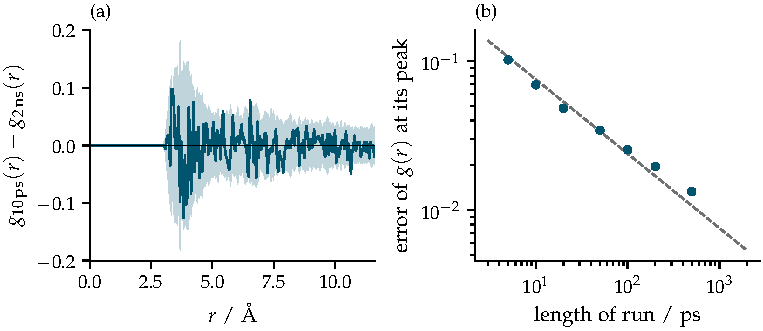
\includegraphics{ch16_observables/rdf_error}
\caption{(a) The radial distribution function of liquid argon from the
first \SI{10}{\pico\second} of Chapter~15's run, less that from all
\SI{2}{\nano\second}, with twice its standard error from the 20 frames
\SI{500}{\femto\second} apart (band). (b) The standard error of $g$ at its
first peak, in bins of \SI{0.05}{\angstrom}, against the length of run
used: predicted from one frame's
spread and the statistical inefficiency (dashed), and measured as the
scatter of independent pieces (points).}
\label{fig:ob-rdf-error}
\end{figure}

\begin{keyidea}
The radial distribution function $g(r)$ counts the partners at the
distance $r$ from an atom against an even scatter. It is a histogram of
pair distances divided by $N\rho$ times the volume of each shell, out to
half the cell, and tends far away to $1 - 1/N$ for atoms placed at random
and to $1 - S(0)/N$, nearly 1, in a liquid in a large enough cell. Its
peaks give the shells of neighbours, its integral the coordination
number, and with the pair potential the energy and the pressure. Its
memory is short, so it converges several times sooner than the
pressure.
\end{keyidea}

\notebook{16}{grow shells around an atom and watch the histogram become g(r)}

\begin{selfcheck}
A gas of 500 atoms placed independently at random in a fixed cell is
analysed with ASE's
normalisation. What value should $g(r)$ approach far from any atom, and
why does a larger cell bring it closer to 1?
\end{selfcheck}

%=============================================================================!
% 16.2  WHAT DIFFRACTION SEES                                                 !
%=============================================================================!
\section{What diffraction sees}
\label{sec:ob-sq}

A street lamp seen through a fine net curtain shows a pattern of bright
spots: light passing between the threads is scattered from each gap, and
in some directions the waves from all the gaps arrive in step and add,
while in others they arrive out of step and cancel. The pattern is set by
the spacing of the threads, and from it the spacing can be read without
looking at the curtain. X-rays and neutrons scattered by the atoms of a
liquid or a crystal do the same at the scale of ångströms, and what they
measure is the structure factor, the counterpart of $g(r)$ in waves.

\subsection*{Waves scattered by atoms}

A plane wave of wave vector $\vb{k}$ has the phase $\vb{k}\cdot\vb{r}$ at
the point $\vb{r}$, its crests lying where that is a multiple of $2\pi$.
Scattered by an atom at $\vb{r}_j$ towards a distant detector, it leaves
as a wave of the same wavelength, its wave vector $\vb{k}'$ of the same
length as $\vb{k}$ and pointing at the detector. The incoming wave
reaches the atom with the phase $\vb{k}\cdot\vb{r}_j$; the path on to the
detector is shorter than the path from the origin by the length of
$\vb{r}_j$ along $\vb{k}'$, which takes off the phase
$\vb{k}'\cdot\vb{r}_j$. So the wave arrives with the phase
$\vb{k}\cdot\vb{r}_j - \vb{k}'\cdot\vb{r}_j$ plus a part that is the same
for every atom, and the waves from different atoms differ in phase by
$-\vb{G}\cdot\vb{r}_j$, with $\vb{G} = \vb{k}' - \vb{k}$ the scattering
vector. The wave from atom $j$ can be drawn as an arrow of unit length
turned through that angle, and the total as the sum of $N$ such arrows.
Turning every arrow the other way changes no length, so the angles may
be taken as $+\vb{G}\cdot\vb{r}_j$, and the total has the components
\begin{equation*}
   \mathcal{C}(\vb{G}) = \sum_j\cos(\vb{G}\cdot\vb{r}_j) , \qquad
   \mathcal{S}(\vb{G}) = \sum_j\sin(\vb{G}\cdot\vb{r}_j) ,
\end{equation*}
the sums of \cref{sec:md-ewald} with every charge 1. A detector
measures the intensity, which grows as the square of a wave's height,
here the square of the total's length; per atom it is the structure
factor
\begin{equation}
   S(\vb{G}) = \frac1N\Bigl[\mathcal{C}(\vb{G})^2 + \mathcal{S}(\vb{G})^2
   \Bigr] .
   \label{eq:ob-sq}
\end{equation}
Expanding the squares and using $\cos A\cos B + \sin A\sin B = \cos(A -
B)$ (\cref{eq:mo-addition}) writes it as a double sum,
\begin{equation*}
   S(\vb{G}) = \frac1N\sum_i\sum_j\cos\bigl(\vb{G}\cdot(\vb{r}_j -
   \vb{r}_i)\bigr) = 1 + \frac1N\sum_i\sum_{j\neq i}\cos(\vb{G}\cdot
   \vb{r}_{ij}) ,
\end{equation*}
the terms with $j = i$ each being 1. Atoms placed at random give cross
terms that average to zero, so $S(\vb{G}) = 1$; atoms of a crystal at a
vector $\vb{G}$ that makes every $\vb{G}\cdot\vb{r}_{ij}$ a multiple of
$2\pi$ give $S(\vb{G}) = N$, a Bragg peak. Such vectors form the
crystal's reciprocal lattice, built as in \cref{sec:md-ewald} on the
crystal's own repeating unit instead of the simulation cell. A liquid has
$S(\vb{G})$ above 1 near the repeat of its shells of neighbours and below
1 elsewhere.

In a periodic cell only waves that repeat with the cell are allowed, the
vectors $\vb{G} = m_1\vb{a}^* + m_2\vb{b}^* + m_3\vb{c}^*$ of
\cref{sec:md-ewald}, the shortest of length $2\pi/L$ for a cube of side
$L$. The function \texttt{structure\_factor} of \texttt{mdlab} evaluates
\cref{eq:ob-sq} on each of them, averages over the frames and over the
vectors of each length $G$, which in a liquid differ only by noise, and
returns $S(G)$ against $G$.

\subsection*{The structure factor from the arrangement}

The double sum can also be written with $g(r)$. Around each atom of a
liquid, which has no preferred direction, \cref{eq:ob-rdf} spreads its
$\rho g(r)\,4\pi r^2\,\dd r$ partners evenly over the shell, so it puts
$\rho g(r)\,\dd^3r$ in each small volume $\dd^3r$ at the separation
$\vb{r}$, and the mean of the double sum is
\begin{equation*}
   S(\vb{G}) = 1 + \rho\int g(r)\cos(\vb{G}\cdot\vb{r})\,\dd^3r
   = 1 + \rho\int\bigl[g(r) - 1\bigr]\cos(\vb{G}\cdot\vb{r})\,\dd^3r ,
\end{equation*}
the second form subtracting $\rho\int\cos(\vb{G}\cdot\vb{r})\,\dd^3r$,
which is zero over the cell for every allowed $\vb{G} \neq \vb{0}$
(\cref{sec:md-ewald}), and which makes the integrand vanish far away
where $g(r)$ is 1. On a shell of radius $r$, with $\theta$ the angle
between $\vb{r}$ and $\vb{G}$, the part at angles between $\theta$ and
$\theta + \dd\theta$ is a band of radius $r\sin\theta$ and width
$r\,\dd\theta$, of area $2\pi r^2\sin\theta\,\dd\theta$, out of $4\pi
r^2$, so the average of the cosine over the shell is, with $u =
\cos\theta$ and $\dd u = -\sin\theta\,\dd\theta$, the minus sign turning
the limits $u = 1$ to $-1$ round,
\begin{equation*}
   \frac12\int_0^\pi\cos(Gr\cos\theta)\sin\theta\,\dd\theta
   = \frac12\int_{-1}^{1}\cos(Gru)\,\dd u
   = \frac12\Bigl[\frac{\sin Gru}{Gr}\Bigr]_{-1}^{1}
   = \frac{\sin Gr}{Gr} .
\end{equation*}
The volume integral is then one over shells,
\begin{equation}
   S(G) = 1 + 4\pi\rho\int_0^\infty r^2\bigl[g(r) - 1\bigr]
   \frac{\sin Gr}{Gr}\,\dd r ,
   \label{eq:ob-sq-rdf}
\end{equation}
which depends only on the length $G$, as it must in a liquid that has no
preferred direction.

\Cref{fig:ob-sq}(a) compares the two routes for liquid argon at
\SI{135}{\kelvin}. From the positions, on 250 frames of the
\SI{2}{\nano\second} run, $S(G)$ has its first peak of 2.271 at $G =
\SI{1.985}{\per\angstrom}$. That peak lies near the repeat of the shells
of neighbours: the first three peaks of $g(r)$ lie at 3.68, 7.04 and
\SI{10.30}{\angstrom}, \SI{3.31}{\angstrom} apart on average, and
$2\pi/3.31 = \SI{1.90}{\per\angstrom}$, 4\% below the peak. Through
\cref{eq:ob-sq-rdf}, with $g(r)$ known only to half the cell, the peak is
2.126, 0.15 below, and at the smallest allowed $G$,
\SI{0.270}{\per\angstrom}, the positions give 0.058 and the transform
0.074, with ripples on either side that take it as low as $-0.05$, which
no intensity can be. Stopping the integral at $L/2$ cuts off whatever
$g(r) - 1$ holds beyond. Near the peak the oscillations of $g(r)$ beyond
the cut keep step with $\sin Gr$, so what is cut off adds up: the $g(r)$
of the 2048-atom runs, stopped at \SI{11.6}{\angstrom} and at
\SI{23.3}{\angstrom}, gives 2.116 and 2.240 there. At small $G$ the loss
is smaller but large beside $S(G)$ itself. The direct route has no such
error and is the one to trust wherever the two differ.

\subsection*{The long-wave limit and the compressibility}

As $G$ shrinks towards 0, $\sin(Gr)/Gr$ tends to 1 and
\cref{eq:ob-sq-rdf} tends to $S(0) = 1 + \rho\int[g(r) - 1]\,\dd^3r$; at
$\vb{G} = \vb{0}$ itself \cref{eq:ob-sq} gives $N$, the beam that passes
straight through, so $S(0)$ means this limit. The same integral measures
how much the number of atoms $N_{\mathrm r}$ in a region of volume
$V_{\mathrm r}$ fluctuates. The
ordered pairs of distinct atoms both inside the region number $N_{\mathrm r}(N_{\mathrm r} -
1)$. Each atom inside has on average $\rho g(r)\,\dd^3r$ partners in each
small volume at the separation $\vb{r}$, and for a region large against
the reach of $g(r) - 1$ nearly every atom is far from its surface, so
\begin{equation*}
   \ens{N_{\mathrm r}(N_{\mathrm r} - 1)}
   = \ens{N_{\mathrm r}}\,\rho\int_{V_{\mathrm r}}g(r)\,\dd^3r
   = \ens{N_{\mathrm r}}\Bigl[\rho\int\bigl[g(r) - 1\bigr]\dd^3r
   + \ens{N_{\mathrm r}}\Bigr] ,
\end{equation*}
since $\rho\int_{V_{\mathrm r}}\dd^3r$ is $\rho V_{\mathrm r} =
\ens{N_{\mathrm r}}$. Subtracting $\ens{N_{\mathrm r}}^2 -
\ens{N_{\mathrm r}}$ from both sides leaves $\operatorname{var}(N_{\mathrm r}) = \ens{N_{\mathrm r}}[1
+ \rho\int[g(r) - 1]\,\dd^3r]$, so $S(0) = \operatorname{var}(N_{\mathrm r})/
\ens{N_{\mathrm r}}$. That fluctuation follows from Chapter~14. A fixed number of
atoms held at fixed pressure has $\operatorname{var}(V) =
\kB T\ens{V}\kappa_T$ (\cref{eq:pr-volume}), and so has a group of atoms
inside a large liquid, the liquid around it acting as the barostat. Such
a group of $N_{\mathrm r}$ atoms has the density $N_{\mathrm r}/V$, which
changes by $\delta\rho/\rho = -\delta V/V$ as its volume $V$ fluctuates;
the region of fixed volume $V_{\mathrm r}$ has the density $N_{\mathrm
r}/V_{\mathrm r}$, which changes by $\delta\rho/\rho = \delta N_{\mathrm
r}/N_{\mathrm r}$ as its number fluctuates. Both are the fluctuation of the
liquid's density over the same volume, so
\begin{equation*}
   \frac{\operatorname{var}(N_{\mathrm r})}{\ens{N_{\mathrm r}}^2} =
   \frac{\operatorname{var}(V)}{\ens{V}^2} = \frac{\kB T\kappa_T}{\ens{V}} ,
   \qquad
   S(0) = \frac{\operatorname{var}(N_{\mathrm r})}{\ens{N_{\mathrm r}}} = \rho\kB T\kappa_T ,
\end{equation*}
the second following on multiplying the first by $\ens{N_{\mathrm r}} =
\rho\ens{V}$. With Chapter~14's $\kappa_T = (1.46 \pm
0.11)$\,\si{\per\giga\pascal}, from the slope $\dd P/\dd V$ of runs at fixed
volume near \SI{0.1}{\giga\pascal}, $\rho\kB T\kappa_T = 0.0554 \pm
0.0042$.

The 256-atom cell has only four lengths of wave vector below
\SI{0.6}{\per\angstrom}, too few to follow $S(G)$ towards $G = 0$, so
\cref{fig:ob-sq}(b) uses Chapter~15's runs of 1372 and 2048
atoms, two of each, whose cells allow $G$ down to
\SI{0.135}{\per\angstrom}. Each value carries the standard error of its
frames' values. A straight line in $G^2$ through the 29 values below
\SI{0.6}{\per\angstrom}, fitted as in \cref{sec:cv-size} with each squared
miss divided by the square of that value's error, reaches $S(0) = 0.0589$
at $G = 0$. The sum of its squared misses in units of the errors is 72,
where scatter alone gives $27 \pm 7$ for 29 values less the two fitted
numbers, so the errors understate the misses by about $\sqrt{72/27} =
1.63$, and the line's error, 0.0002, enlarged by that factor becomes
0.0004. The two values, $0.0589 \pm 0.0004$ from the positions and
$0.0554 \pm 0.0042$ from the change of pressure with volume, lie 0.8
combined errors apart: the long waves of the structure and the liquid's
stiffness against squeezing measure the same compressibility. The test
is loose in one respect: Chapter~14 took its slope at a volume 2.2\%
smaller than this run's, where the denser liquid is the stiffer.

The same integral fixes the far value of $g(r)$ in a fixed cell
(\cref{sec:ob-rdf}). With the divisor $N\rho$, an atom's partners over
the whole cell number $N - 1$, so $\rho\int_V[g(r) - 1]\,\dd^3r = -1$. In a
cell large enough for $g(r) - 1$ to die away well inside it, the part of
the integral near the atom is $S(0) - 1$, and the remaining $-S(0)$ is
spread over the rest of the cell, where $g(r) - 1$ is then $-S(0)/\rho V =
-S(0)/N$\cite{Lebowitz1961}: $1 - 1/N$ for atoms at random, whose $S(0)$
is 1, and $1 - 0.059/N$ for this liquid. In the corners of the 2048-atom
cell the partners fall short of $\rho$ by a fraction $(3.3 \pm
0.5)\times10^{-5}$, which is $S(0)/N$ for $S(0) = 0.067 \pm 0.009$, the
value above within its error.

\begin{figure}[htb]
\centering
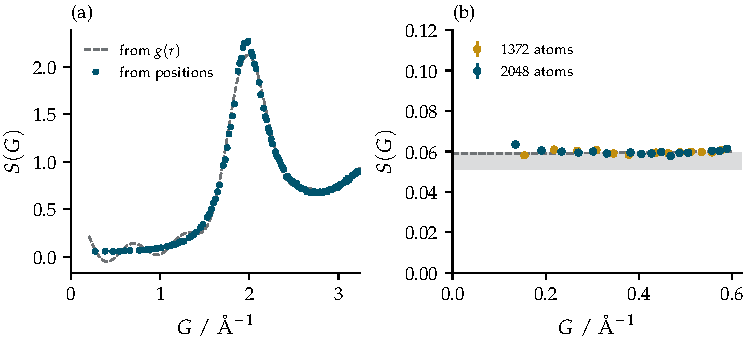
\includegraphics{ch16_observables/sq}
\caption{(a) The structure factor of liquid argon at \SI{135}{\kelvin}
from the positions, averaged over the wave vectors of the 256-atom cell
of each length up to $12\times2\pi/L = \SI{3.24}{\per\angstrom}$ (points),
against the
transform of $g(r)$ cut at half the cell (dashed). (b) $S(G)$ at the
smallest wave vectors of the 1372- and 2048-atom runs of Chapter~15, two
runs of each, with their standard errors, and a straight line in $G^2$
fitted below \SI{0.6}{\per\angstrom} (dashed), against $\rho\kB T\kappa_T$
with Chapter~14's compressibility (band, its error).}
\label{fig:ob-sq}
\end{figure}

\begin{keyidea}
The structure factor $S(G) = [\mathcal{C}^2 + \mathcal{S}^2]/N$ is the
intensity, per atom, of waves scattered with the change of wave vector
$\vb{G}$, and what diffraction measures. It is the transform of
$g(r) - 1$ by $\sin(Gr)/Gr$, which a cut at half the cell spoils, by
0.15 at the peak and by a large fraction at small $G$, so it is computed
from the positions on the cell's own wave vectors. Its limit at $G = 0$ is $\rho\kB T\kappa_T$.
\end{keyidea}

\notebook{16}{compare S(G) from the positions and from g(r)}

\begin{selfcheck}
For a crystal at $T = 0$, what is $S(\vb{G})$ at a vector $\vb{G}$ of
its reciprocal lattice, and at a vector of the cell that is not one of
them?
\end{selfcheck}

%=============================================================================!
% 16.3  BONDS AND MOLECULES                                                   !
%=============================================================================!
\section{Bonds and molecules}
\label{sec:ob-bonds}

To follow a reaction, we must first decide which atoms form each
molecule. We assign bonds to pairs, then collect atoms joined through
those bonds into molecules. A distance cutoff gives a first rule, but
thermal vibrations can carry a pair across it repeatedly without a
chemical change. This section introduces a bond criterion that retains
that distinction, then uses the resulting graph to identify molecules
and species.

\subsection*{A bond from a distance}

The forces of most models say nothing about bonds: they are functions of
the positions. A bond is therefore assigned from the distance between
two atoms, and a common yardstick is the sum of their covalent radii,
$R_i + R_j$, from a table of radii for each element such as the one ASE
carries\cite{Larsen2017}: two carbon atoms ($R = \SI{0.76}{\angstrom}$
each) are bonded within some multiple of \SI{1.52}{\angstrom}. Read
literally, such a rule makes a bond flicker. A bonded pair vibrates, and
if the far end of its vibration lies near the cutoff, each vibration
carries it out and back across it, two events per period with nothing
chemical happening.

The cure is a band of hysteresis, as in a thermostat that switches the
heating on below one temperature and off above a higher one. A pair not
yet bonded becomes bonded when it comes closer than $r_{\mathrm{on}}$; a
bonded pair stays bonded until it parts beyond $r_{\mathrm{off}} >
r_{\mathrm{on}}$. A vibration whose whole swing, from its near end to its
far end, is narrower than the band cannot carry the pair across both
distances, so it cannot make a bond flicker, while a real dissociation,
which carries the atoms apart for good, crosses both. \texttt{mdlab.bonds.BondTracker} takes
$r_{\mathrm{on}}$ and $r_{\mathrm{off}}$ as 1.2 and 1.4 times the sum of
the covalent radii unless told otherwise, factors that bracket the first
minimum of $g(r)$ for carbon (\cref{sec:ob-reactions}); for a model, or
for any pair of elements, the two distances can be given directly.

To measure the effect we use a model gas built to react. Two kinds of
atom, A and B, of nitrogen's mass, attract each other through the Morse
well of \cref{sec:pe-pairs} with depth $D_{\mathrm M} = \SI{1}{\electronvolt}$,
width $a_{\mathrm M} = \SI{2}{\per\angstrom}$ and $r_0 = \SI{1.2}{\angstrom}$, the $D$
and $a$ of that section marked here to keep them apart from the
diffusion coefficient and the lattice spacing of later sections; two atoms of
the same kind only repel, as $D_{\mathrm M}\mathrm{e}^{-2a_{\mathrm M}(r - 2.6\,\text{\AA})}$, which
weakens a second partner's hold: a line B-A-B with both bonds at
\SI{1.48}{\angstrom} lies only \SI{0.40}{\electronvolt} below AB and a free
B, so such complexes form but soon part. The constants are chosen for
illustration and are not fitted to any real pair of atoms. 250 molecules
AB in a cubic cell of side \SI{63}{\angstrom} are held at 1500, 1750,
2000, 2250 and \SI{2500}{\kelvin} by Langevin friction of \SI{1}{\per\pico\second}, which
stands for a buffer gas that supplies and removes energy, for
\SI{100}{\pico\second} each. A bond forms where the pair's energy falls
below $-D_{\mathrm M}/2$, at $r_{\mathrm{on}} = \SI{1.814}{\angstrom}$, and breaks
where it rises above $-D_{\mathrm M}/8$, at $r_{\mathrm{off}} = \SI{2.570}{\angstrom}$.
A molecule's small vibrations have the period $2\pi\sqrt{m_{\mathrm r}/2D_{\mathrm M}a_{\mathrm M}^2}
= \SI{59.8}{\femto\second}$ (\cref{sec:os-small,sec:os-bodies}), with
$m_{\mathrm r} = \SI{7.0035}{\amu}$ the reduced mass and $2D_{\mathrm M}a_{\mathrm M}^2 =
\SI{8}{\electronvolt\per\angstrom\squared}$ the stiffness of the well.

At \SI{2000}{\kelvin} a single cutoff at $r_{\mathrm{on}}$ records 53\,265
bonds formed or broken in \SI{100}{\pico\second}; the band records 16\,442,
3.2 times fewer (\cref{fig:ob-bonds}a). Many of the remaining events are
not flicker either: an A and a B that meet with too much energy to stay
together pass through each other's well and part again within a
vibration or two. Requiring that a bond last a set time before its
forming and breaking count, and likewise that a pair which parts stay
apart that long, and dropping both events of any bond or gap shorter than
that (\texttt{bonds.persistent}), removes these passing encounters and the
flicker the band leaves. For a least lifetime of \SI{0.5}{\pico\second}
the counts fall to \num{5501} with the single cutoff and \num{6548} with
the band, which then keeps a fifth more. The remaining events fall
more slowly as the least lifetime grows, by 40\% and 36\% from 0.5 to
\SI{2}{\pico\second}, against a fall by 9.7 and 2.5 times from no least
lifetime to \SI{0.5}{\pico\second}: they are the molecules that form and
break.

\subsection*{Keys and set differences}

Each bond is stored as one whole number, its key $iN + j$ for the
atoms $i < j$. Different pairs have different keys, since $j < N$, and
the atoms are recovered as the quotient and the remainder of the key
divided by $N$. A computer stores such numbers in 64 binary digits, bits,
reaching $2^{63} \approx \num{9.2e18}$ with one bit for the sign, so keys
fit for $N$ up to about $3\times10^9$, and about $2\times10^9$ once the
tracker doubles each key (below). The
bonds formed between two frames are the keys in the new set and not in
the old, and those broken the keys in the old and not in the new.

\begin{toolbox}[Set differences of sorted lists]
Two lists of whole numbers, each sorted and without repeats, can be
compared in one pass. A pointer starts at the head of each. If the two
numbers under the pointers are equal, the number is in both lists, and
both pointers move on; otherwise the smaller is in its own list only,
and only its pointer moves. When one list is used up, the rest of the
other is in that list only. Each step moves at least one pointer, so for
lists of lengths $n_1$ and $n_2$ the pass takes at most $n_1 + n_2$
steps, against $n_1n_2$ for testing every pair. \texttt{BondTracker.update} merges this way
the sorted keys within $r_{\mathrm{off}}$ of the new frame with the
sorted bonds of the last one: a key in both is kept, a key only in the new
list is a new bond if it lies within $r_{\mathrm{on}}$, and a key only in
the old list is a bond broken.
\end{toolbox}

The candidates are the pairs that the force evaluation has already
found, which the model of \texttt{md.PairModel} keeps with their
distances after each call, so the tracker measures no distance of its
own; this serves as long as the cutoff of the forces reaches the largest
$r_{\mathrm{off}}$. Most candidates lie beyond the largest
$r_{\mathrm{off}}$ and are passed over at once; the rest are sorted, each
stored as twice its key plus 1 if the pair is within $r_{\mathrm{on}}$, so
that one sort orders the keys, and halving, the remainder dropped,
recovers each key, the remainder its flag; then they are merged:

\begin{code}
    def update(
        self, i: ArrayLike, j: ArrayLike, dist: ArrayLike
    ) -> tuple[NDArray, NDArray]:
        # the keys within r_off, each carrying its "closer than r_on" flag
        # in an extra lowest bit, so that one sort orders both
        packed = np.sort(_jit(_held_keys)(
            np.asarray(i, dtype=np.int64), np.asarray(j, dtype=np.int64),
            np.asarray(dist, dtype=float), self.kind, self.r_on, self.r_off,
            self._reach, self.n))
        self.keys, formed, broken = _jit(_merge)(
            packed >> 1, (packed & 1).astype(np.bool_), self.keys)
        return formed, broken
\end{code}

\noindent The two helpers are plain loops, the filter and the merge of the
toolbox, compiled by Numba as in \cref{sec:md-speed}.

\subsection*{Molecules}

A molecule is a set of atoms joined to one another through chains of
bonds.

\begin{toolbox}[Graphs and their connected components]
A graph is a set of nodes and a set of edges, each edge joining two
nodes. Here the atoms are the nodes and the bonds the edges. A graph of
$N$ nodes can be stored as its adjacency matrix, $N\times N$, with 1 in
row $i$ and column $j$ when $i$ and $j$ are joined and 0 otherwise. For
atoms nearly every entry is 0, since each atom has a few bonds, so only
the positions of the ones are stored, a sparse matrix whose storage grows
as the number of bonds, not as $N^2$. A connected component is a largest
set of nodes any two of which are joined by a path of edges. It is found
by a search, which starts from any node not yet assigned, adds its
neighbours, then their neighbours, and so on until no new node is
reached; those nodes are one component, and the search starts again from
a node not yet assigned. Each edge is followed at most twice, so the work grows
as the number of nodes plus edges.
\end{toolbox}

\noindent \texttt{mdlab.bonds.molecules} builds the sparse matrix of the
bonds and labels each atom with its component through
\texttt{scipy.sparse.csgraph}:

\begin{code}
def molecules(n_atoms: int, keys: ArrayLike) -> NDArray:
    i, j = np.divmod(np.asarray(keys, dtype=np.int64), n_atoms)
    graph = coo_matrix((np.ones(len(i)), (i, j)), shape=(n_atoms, n_atoms))
    return connected_components(graph, directed=False)[1]
\end{code}

\subsection*{Species}

Two molecules belong to the same species if they have the same atoms
bonded in the same way, whatever the numbers the atoms carry in the run.
The formula is the first part of the name: the number of atoms of each
element, written in the Hill order: in a molecule with carbon, carbon
first, then hydrogen, then the others alphabetically, and in one without,
all of them alphabetically, so that a molecule of two A and one B is
A$_2$B.
The formula does not tell isomers apart, molecules of the same atoms
bonded differently, such as a ring of six carbon atoms and a chain of
six.

\begin{toolbox}[Hashing and canonical labels]
A hash is a function that turns data of any size into a number of fixed
size, such that equal data give equal numbers and different data give
different numbers with high probability: a fingerprint. Two molecules
should get the same number if one can be renumbered into the other. A
label that does not change under renumbering is called canonical; sums
over the atoms are canonical, since the order of the terms does not
change a sum. \texttt{mdlab.bonds.graph\_hash} builds one in rounds, after
Weisfeiler and Lehman. Each atom starts with a number for its element,
scrambled by a fixed function that spreads nearby numbers far apart. In
each round it replaces its number by the scrambled combination of its own
number and the sum of its neighbours' scrambled numbers, so that after
$m$ rounds the number describes the atom's surroundings $m$ bonds deep,
and the molecule's number is the sum over its atoms. In a ring of six
every atom has two neighbours with two neighbours each, all round; at the
ends of a chain an atom has one, and its number differs from the first
round on. The scheme is not perfect. Graphs in which every atom has the
same number of neighbours of the same kinds, such as a triangular prism of
six atoms and a hexagon of six whose opposite atoms are also joined, look
alike to every round and get the same number, so two species can, rarely,
share a hash.
\end{toolbox}

\noindent The scrambling is the finishing step of the generator
splitmix64, a few multiplications and shifts of 64-bit whole numbers whose
sums are kept to their lowest 64 bits, dropping whatever passes
$2^{64}$; four rounds are used. \texttt{ReactionLog}
names each species by its formula, and a further isomer of a formula
already seen by the formula with a prime, A$_2$B$'$, in order of
appearance.

\subsection*{Checks}

The tracker's first frame, with no hysteresis yet, must find the pairs
closer than the sum of their radii, as ASE's \texttt{neighbor\_list} does
with its \texttt{natural\_cutoffs}. On 80 atoms of carbon and hydrogen at
random in a periodic cell, with $r_{\mathrm{on}}$ the sum of the radii,
the two lists are identical,
and both equal the list from testing every pair. Over 40 frames of atoms
moving at random, the tracker's bonds equal, frame by frame, those of a
direct transcription of the rule. On invented trajectories whose events
are known, it finds them all: of two molecules N$_2$, one pulled apart gives N$_2$
$\to$ N + N; one of the freed atoms brought to the other molecule gives N
+ N$_2$ $\to$ N$_3$; a ring of six carbon atoms, one of whose bonds is
stretched beyond $r_{\mathrm{off}}$, becomes a chain whose hash differs,
C$_6$ $\to$ C$_6'$. Each is a test of \texttt{mdlab}.

\begin{figure}[htb]
\centering
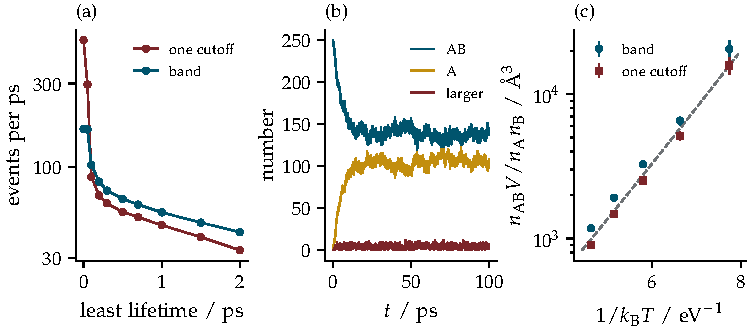
\includegraphics{ch16_observables/bonds}
\caption{The A-B gas: 250 molecules in a cell of side \SI{63}{\angstrom}
under Langevin friction of \SI{1}{\per\pico\second} for
\SI{100}{\pico\second}. (a) Bonds formed or broken per picosecond at
\SI{2000}{\kelvin}, counted with a single cutoff at $r_{\mathrm{on}}$ and
with the band from $r_{\mathrm{on}}$ to $r_{\mathrm{off}}$, against the
least lifetime an event must have to count. (b) The numbers of molecules
AB, of free A and of larger complexes at \SI{2000}{\kelvin} against time.
(c) The equilibrium constant $n_{\mathrm{AB}}V/n_{\mathrm A}n_{\mathrm B}$
over the last \SI{90}{\pico\second} with the band (circles) and with the
single cutoff (squares), with the standard error of nine blocks, against
$\int_0^{r_{\mathrm{on}}}4\pi r^2\mathrm{e}^{-\beta\varphi}\,\dd r$
(dashed).}
\label{fig:ob-bonds}
\end{figure}

\begin{keyidea}
A bond is assigned from the distance, with a band of hysteresis, forming
below $r_{\mathrm{on}}$ and breaking above $r_{\mathrm{off}}$, and events
are counted only for bonds and gaps that last a least time. Bonds are whole-number
keys, and those formed and broken are differences of sorted lists.
Molecules are the connected components of the graph of bonds, and a
species is named by its formula and a hash of its graph that does not
depend on the numbering.
\end{keyidea}

\notebook{16}{watch bonds flicker with one cutoff and settle with a band}

\begin{selfcheck}
In a run of 1000 atoms, the bond between atoms 17 and 342 has the key
17\,342. Which bond has the key 342\,017?
\end{selfcheck}

%=============================================================================!
% 16.4  REACTIONS AND THEIR RATES                                             !
%=============================================================================!
\section{Reactions and their rates}
\label{sec:ob-reactions}

Once molecules have been identified, a reaction is a change in which
molecules a group of atoms belongs to. We record the reactants and
products, then turn repeated events into rates. The uncertainty depends
on the number of independent events, rather than the number of saved
frames. We also measure the cost of doing this analysis during a run.

\subsection*{Reactions from changes of species}

Between two frames, each atom belongs to a molecule before and to a
molecule after. Joining each old molecule to each new one that shares an
atom with it gives a graph whose nodes are molecules, and its connected
components are the reactions. A molecule that kept its atoms and its
bonds is one old node joined to one new node with the same hash, and is
passed over; every other component is a reaction, its old molecules the
reactants and its new ones the products. A ring that opens is a
component of one old and one new molecule with different hashes, C$_6$
$\to$ C$_6'$; two molecules that exchange an atom, AB + B $\to$ B + AB, are
a component of two old and two new molecules with the same names.
\texttt{mdlab.bonds.ReactionLog} does this frame by frame, recording the
time, the reactants and the products of each reaction, and the counts of
each species.

In the A-B gas at \SI{2000}{\kelvin} the 250 molecules AB lose partners
at first (\cref{fig:ob-bonds}b), and after the first \SI{10}{\pico
\second} the gas holds on average 139.3 AB, 104.1 free A and 103.9 free B,
with 2.2 AB$_2$, 1.9 A$_2$B and a few larger complexes.
Over \SI{100}{\pico\second} the log holds 57 kinds of reaction. The most
frequent, counting every event with the band and no least lifetime, are
\begin{center}
\begin{tabular}{@{}lr@{\qquad}lr@{}}
AB $\to$ A + B & 4517 & A + B $\to$ AB & 4421\\
AB + B $\to$ AB$_2$ & 1618 & AB$_2$ $\to$ AB + B & 1602\\
A + AB $\to$ A$_2$B & 1556 & A$_2$B $\to$ A + AB & 1566\\
AB + AB $\to$ A$_2$B$_2$ & 301 & A$_2$B$_2$ $\to$ AB + AB & 298
\end{tabular}
\end{center}
a reaction network: a graph whose nodes are the species and the
reactions, each reaction joined to its reactants and its products and
carrying its count. Each reaction and its reverse occur
nearly equally often, as every process in a gas at equilibrium is
balanced by its reverse: AB $\to$ A + B outnumbers its reverse by 96, about
the 111 net breaks by which the molecules fell from 250 to 139.3 at the
start, and the others differ by less than the $\sqrt n$ of the toolbox
below. The complexes are brief. In a steady state the complexes present
at any moment are those formed within one lifetime before it, so their
number is the rate at which they form times the lifetime. AB$_2$ forms
16.8 times per picosecond and 2.18 are present on average, so each lasts
$2.18/16.8 = \SI{0.130}{\pico\second}$; A$_2$B lasts
\SI{0.120}{\pico\second}. They are passing
encounters of the kind the least lifetime of \cref{sec:ob-bonds} removes.

\begin{toolbox}[Rates from counts, and the Poisson distribution]
Events that happen independently, at a steady rate $\nu$ for each of
many molecules, are counted over an exposure $X$, the sum over the
molecules of the time each was able to react. Cut into $J$ small pieces,
the exposure has in each an event with the small probability $p = \nu
X/J$ and none otherwise, independently, so the count is a sum of $J$
independent numbers each 0 or 1. Each such number has the mean $p$, and
so does its square, which is the same 0 or 1, so its variance is $p -
p^2 = p(1 - p)$. The count then has the mean $Jp = \nu X$ and, since the
variances of independent numbers add (\cref{sec:cv-mean}), the variance
$Jp(1 - p)$, which tends to $\nu X$ as the pieces shrink. The rate is
estimated as $n/X$, with the standard error $\sqrt n/X$, a fraction
$1/\sqrt n$ of itself: a rate from 100 events is known to a tenth, from
10\,000 to a hundredth. The chance of $n$ events is the number of ways of
choosing $n$ of the $J$ pieces, $J(J - 1)\cdots(J - n + 1)/n!$, times
$p^n(1 - p)^{J - n}$, which with $p = \nu X/J$ is
\begin{equation*}
   \frac{J(J - 1)\cdots(J - n + 1)}{J^n}\,\frac{(\nu X)^n}{n!}\,
   \Bigl(1 - \frac{\nu X}{J}\Bigr)^{J - n} .
\end{equation*}
As $J$ grows with $n$ fixed, the first fraction, a product of $n$
factors each tending to 1, tends to 1, and the logarithm of the last
factor, $(J - n)\ln(1 - \nu X/J)$, tends to $-\nu X$, since $\ln(1 + y)$
is $y$ plus terms of order $y^2$ (\cref{sec:th-langevin}). The chance
tends to the Poisson distribution
\begin{equation*}
   \mathcal{P}(n) = \frac{(\nu X)^n}{n!}\,\mathrm{e}^{-\nu X} ,
\end{equation*}
whose mean and variance are both $\nu X$, the limits of the count's.
\end{toolbox}

\noindent Counted events of a run can be correlated, a bond that breaks
and re-forms twice counting thrice; the least lifetime of
\cref{sec:ob-bonds} removes most of these. At \SI{2000}{\kelvin}, the bonds
broken in 89 windows of \SI{1}{\pico\second} number 33.82 on average with
variance 36.24, a ratio of 1.07, within the 0.15 by which that ratio
scatters over 89 windows of a Poisson count, and their histogram lies
close to the Poisson distribution of the same mean
(\cref{fig:ob-rates}b).

\subsection*{Rates against temperature}

With the band and a least lifetime of \SI{0.5}{\pico\second}, after the
first \SI{10}{\pico\second}, the rate of breaking is the number of bonds
broken divided by the bond-picoseconds of exposure, and the rate constant
of forming the number formed divided by the exposure of free pairs,
$\int n_{\mathrm A}n_{\mathrm B}/V\,\dd t$. At \SI{1500}{\kelvin} 1828 bonds
break over \num{18168} bond-picoseconds, $k_{\mathrm b} = (0.1006 \pm
0.0024)$\,\si{\per\pico\second}, and at \SI{2500}{\kelvin} 3182 over 9500,
$(0.3350 \pm 0.0059)$\,\si{\per\pico\second}; the rate constant of forming
falls over the same range, from $(1911 \pm 45)$ to $(415 \pm
7)$\,\si{\angstrom\cubed\per\pico\second} (\cref{fig:ob-rates}a). A rate
that rises as $\mathrm{e}^{-E_{\mathrm a}/\kB T}$ has a logarithm that
falls on a straight line of slope $-E_{\mathrm a}$ against $1/\kB T$, the
Arrhenius form. The error of the logarithm of a rate from $n$ events is
its fractional error, $1/\sqrt n$, so each point is weighted in the fit
by $\sqrt n$, the misses being measured in units of their errors as in
\cref{sec:cv-size}: breaking has $E_{\mathrm a} = \SI{0.389}{\electronvolt}$
and forming $-\SI{0.478}{\electronvolt}$, a rate that falls as the
temperature rises.

Neither slope is the depth of the well, \SI{1}{\electronvolt}, and they
need not be: each rate depends on how the buffer gas supplies and removes
energy, as Chapter~13 found for hops. Their ratio does not. At
equilibrium forming and breaking balance, $k_{\mathrm f}n_{\mathrm A}
n_{\mathrm B}/V = k_{\mathrm b}n_{\mathrm{AB}}$, so $k_{\mathrm f}/k_{\mathrm
b}$ is the equilibrium constant $K_{\mathrm{eq}} = n_{\mathrm{AB}}V/n_{\mathrm
A}n_{\mathrm B}$ of the counts: 18\,994 against 20\,583
\si{\angstrom\cubed} at \SI{1500}{\kelvin}, 3406 against 3266 at 2000 and
1237 against 1177 at \SI{2500}{\kelvin}, within 8\%. The two are not
the same average. With nearly as many bonds formed as broken,
$k_{\mathrm f}/k_{\mathrm b}$ is the bond-picoseconds over the exposure of
free pairs, 19\,162, 3416 and \SI{1235}{\angstrom\cubed}, a ratio of time
averages that counts the bonds within complexes too, while $K_{\mathrm{eq}}$
averages the ratio of the counts for the molecules AB alone. Since
$\ln K_{\mathrm{eq}} = \ln k_{\mathrm f} - \ln k_{\mathrm b}$, its slope is the
difference of theirs, $0.478 - (-0.389) = \SI{0.867}{\electronvolt}$, and
the counts give \SI{0.912}{\electronvolt}.

That constant can be predicted for a dilute gas of A and B whose only
interaction is the pair potential, with a pair bonded when closer than
$r_{\mathrm{on}}$. Arrangements with $n_{\mathrm{AB}}$ bonded pairs and
with one more, made by joining a free A to a free B, are compared by the
Boltzmann weights of \cref{sec:sm-canonical} integrated over the
positions; the momenta, the same in both, cancel. A free pair, each atom
anywhere, has the weight $V^2$; a bonded pair, its centre anywhere and
its separation within $r_{\mathrm{on}}$, has $V\int_0^{r_{\mathrm{on}}}4\pi
r^2\mathrm{e}^{-\beta\varphi(r)}\,\dd r$. The A and the B to join can be
chosen in $n_{\mathrm A}n_{\mathrm B}$ ways, and each result is reached
from $n_{\mathrm{AB}} + 1$ starting arrangements, one for each of its
bonds, so one more bond is more probable than not by the factor
\begin{equation*}
   \frac{n_{\mathrm A}n_{\mathrm B}}{n_{\mathrm{AB}} + 1}\,\frac1V
   \int_0^{r_{\mathrm{on}}}4\pi r^2\mathrm{e}^{-\beta\varphi(r)}\,\dd r .
\end{equation*}
At the most probable $n_{\mathrm{AB}}$, large enough that $n_{\mathrm{AB}} +
1$ differs little from $n_{\mathrm{AB}}$, the factor is 1, so
$K_{\mathrm{eq}}$ equals the integral, the mass action law. The integral falls
sixteen-fold from \num{15756} to \SI{987}{\angstrom\cubed} between 1500
and \SI{2500}{\kelvin}, and the constant from the single cutoff at
$r_{\mathrm{on}}$, with the standard error of nine blocks, follows it at
1.00, 0.89, 0.92, 0.95 and 0.91 of its value (\cref{fig:ob-bonds}c); the
band, which also keeps pairs between $r_{\mathrm{on}}$ and $r_{\mathrm{off}}$
that were once closer, gives 1.13 to 1.31. The integral treats the free
atoms as an ideal gas, leaving out the attraction between unlike atoms
and the repulsion between like ones beyond $r_{\mathrm{on}}$.

\subsection*{Carbon from the melt}

Carbon's bonds come and go in the melt. 216 atoms at
\SI{2.0}{\gram\per\centi\metre\cubed}, with the potential of
Tersoff\cite{Tersoff1989} through ASE's calculator, the parameters those
that ship with ASE, are held at \SI{6000}{\kelvin} for
\SI{2}{\pico\second} by CSVR with $\tau_{\mathrm T} = \SI{50}{\femto
\second}$, and the thermostat's target is then lowered steadily to
\SI{300}{\kelvin}, over \SI{10}{\pico\second} in one run and
\SI{40}{\pico\second} in another, with steps of \SI{0.5}{\femto\second}.
The model is carried by \texttt{io.AseModel}, which calls any ASE
calculator with the positions and returns the energy and the forces as an
\texttt{mdlab} model does. The default band, 1.2 to 1.4 times twice the
covalent radius of carbon, \num{1.824} to \SI{2.128}{\angstrom}, brackets
the first minimum of $g(r)$ in the melt, at \SI{1.963}{\angstrom}, and
after the quench lies, all but its first \SI{0.03}{\angstrom}, in the gap
from 1.85 to \SI{2.15}{\angstrom} where $g(r)$ is zero
(\cref{fig:ob-carbon}a), so the criterion counts the first shell of
neighbours and nothing beyond. In the melt, between 0.5 and
\SI{2}{\pico\second}, 0.764 of the atoms have three bonds, 0.161 two and
0.071 four, and the bonds form and break continually: after the first
frame there are 1870 events over the faster run and 3479 over the slower,
1221 of each in the first \SI{2}{\pico\second} at \SI{6000}{\kelvin}. As the melt cools the three-fold atoms grow at the expense of
the others, and the last bond forms or breaks when the thermostat's
target has fallen to \SI{2335}{\kelvin} in the faster run and
\SI{2432}{\kelvin} in the slower (\cref{fig:ob-carbon}b). At \SI{300}{\kelvin} the faster quench leaves
0.852 of the atoms with three bonds, 0.065 with two and 0.083 with four;
the slower leaves 0.907, 0.042 and 0.051. Every atom is in one molecule,
the solid itself. These are single runs, so the difference between the
two quenches has no error bar yet; the trend, fewer defects for slower
cooling, is what a repeat would test.

\subsection*{Keeping up with the run}

An analysis can read frames from a file after the run, or watch the run
as it goes. \texttt{io.read\_frames} reads any trajectory file ASE can
read, extended XYZ or ASE's own, converting velocities to
\si{\angstrom\per\femto\second}. Watching needs no file: \texttt{md.run}
and \texttt{thermostats.run} accept observers, functions called at every
recorded frame with the time, the positions and the velocities, and the
pairs that the force evaluation has just found are at hand in
\texttt{PairModel.last\_pairs}, so an observer can feed them to a
\texttt{ReactionLog} without searching for neighbours again. The gas runs
above did so every \SI{10}{\femto\second}.

Such analysis must cost little next to the forces. \Cref{fig:ob-timing}
times one frame's analysis, bonds, molecules, hashes, formulas and
reactions, against one force evaluation of a cheap model, liquid argon's Lennard-Jones forces with the neighbour list already
built, from 864 to \num{97556} atoms. The bonds are taken between atoms
closer than \SI{4.0}{\angstrom}, kept to \SI{4.4}{\angstrom}, 4.4 per atom, a
denser graph than most molecules give. With the two loops of
\cref{sec:ob-bonds} and the rounds of the hash compiled by Numba, and the
pairs taken from the force evaluation, the analysis costs about 0.15 of a
force evaluation at 864 atoms and about 0.10 from \num{10976} atoms up,
in each of two sets of timings. From 864 to \num{97556} atoms, 113 times as
many, both times grow roughly in proportion to $N$, the force
evaluation's somewhat faster. Analysed at a
frame saved every tenth step, the bonds cost about 1\% of the run, and
with any learned potential, whose forces cost far more than these, much
less.

\begin{figure}[htb]
\centering
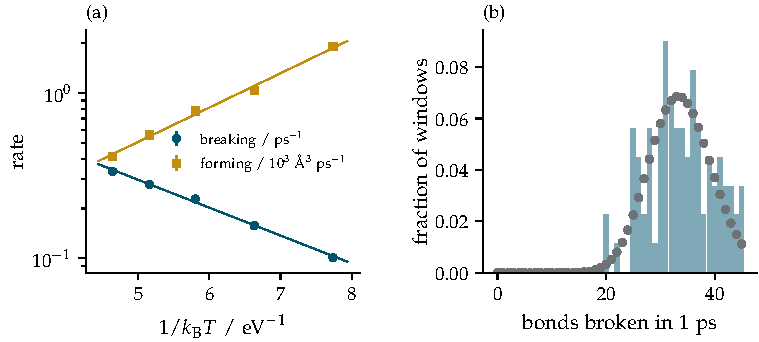
\includegraphics{ch16_observables/rates}
\caption{The A-B gas. (a) The rate of breaking per bond and picosecond
(circles) and the rate constant of forming in \SI{e3}{\angstrom\cubed\per
\pico\second} (squares), counting events of the band that lived at least
\SI{0.5}{\pico\second}, with the error $\sqrt n$ of each count, against
$1/\kB T$, with straight lines fitted to their logarithms. (b) At
\SI{2000}{\kelvin}, the fraction of 89 windows of \SI{1}{\pico\second} in
which a given number of bonds broke (bars), against the Poisson
distribution of the same mean (points).}
\label{fig:ob-rates}
\end{figure}

\begin{figure}[htb]
\centering
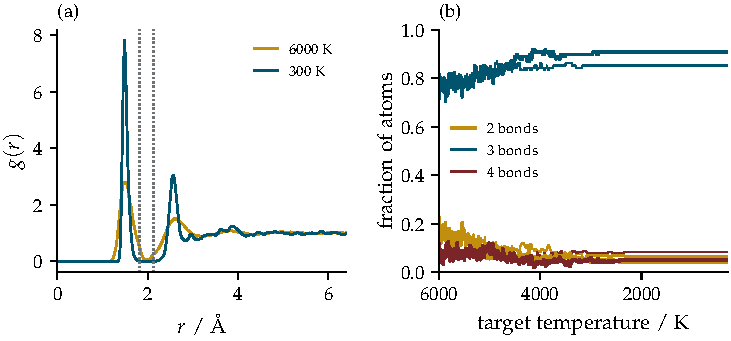
\includegraphics{ch16_observables/carbon}
\caption{216 carbon atoms at \SI{2.0}{\gram\per\centi\metre\cubed} with
Tersoff's potential, quenched from \SI{6000}{\kelvin}. (a) $g(r)$ of the
melt and of the solid after the slow quench, with $r_{\mathrm{on}}$ and
$r_{\mathrm{off}}$ of the default band (dotted). (b) The fractions of atoms
with two, three and four bonds against the thermostat's target, for the
quench over \SI{10}{\pico\second} (thin) and over \SI{40}{\pico\second}
(thick).}
\label{fig:ob-carbon}
\end{figure}

\begin{figure}[htb]
\centering
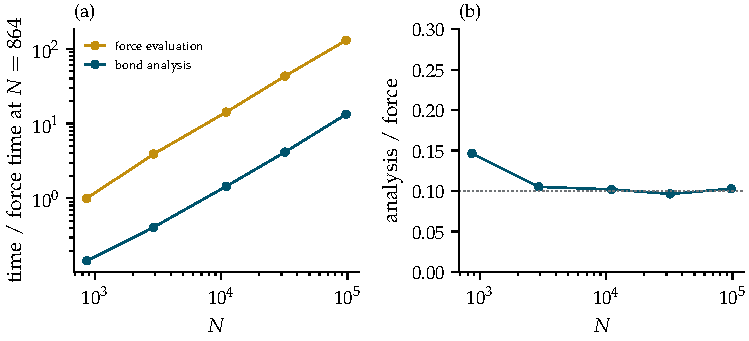
\includegraphics{ch16_observables/timing}
\caption{(a) The time of one force evaluation of liquid argon's model
and of one frame's bond analysis, against the number of atoms, each
relative to the force evaluation of 864 atoms, the least of three tries.
(b) Their ratio, with the tenth that the analysis is meant to stay within
(dotted).}
\label{fig:ob-timing}
\end{figure}

\begin{keyidea}
A reaction is a change of the molecules that some atoms belong to, found
as a connected group of old and new molecules. Rates are counts over
exposures, with the error $\sqrt n$ of a Poisson count; the ratio of the
rate constants of a reaction and its reverse is the equilibrium constant,
which statistical mechanics predicts. Observers analyse the run as it goes,
reusing the force evaluation's pairs, at about a tenth of its cost.
\end{keyidea}

\notebook{16}{count reactions in the gas and put error bars on their rates}

\begin{selfcheck}
A rate is estimated from 25 counted events. To what fraction is it known,
and how many events would halve that?
\end{selfcheck}

%=============================================================================!
% 16.5  HOW FAR ATOMS WANDER                                                  !
%=============================================================================!
\section{How far atoms wander}
\label{sec:ob-msd}

A drop of ink in a glass of still water spreads without any current to
carry it: each grain of dye is knocked about by the molecules around it,
and the cloud of grains widens. No grain goes anywhere in particular, yet
the width of the cloud grows steadily with time. Atoms in a liquid wander
in the same way, and the rate at which the width grows is the diffusion
coefficient, which Chapter~13 measured as a sixth of a slope and promised
to treat properly here.

\subsection*{A random walk}

A walker who takes steps $\vb{s}_1, \vb{s}_2, \dots$, each of random
direction and independent of the others, is at $\vb{r}_n = \vb{s}_1 +
\dots + \vb{s}_n$ after $n$ of them. The square of that sum is the sum of
all products of two steps, so
\begin{equation*}
   \ens{\lvert\vb{r}_n\rvert^2}
   = \sum_{k=1}^n\ens{\lvert\vb{s}_k\rvert^2}
   + \sum_{k\neq l}\ens{\vb{s}_k\cdot\vb{s}_l}
   = n\ens{s^2} ,
\end{equation*}
the cross terms vanishing because independent steps of mean zero have
zero covariance (\cref{sec:cv-correlation}). The mean squared distance
from the start grows in proportion to the number of steps, and so to the
time, while the mean position stays where it began. The diffusion
coefficient $D$ is defined by that growth: for an atom in $d$ directions,
\begin{equation}
   \ens{\lvert\vb{r}(t_0 + t) - \vb{r}(t_0)\rvert^2} \to 2dDt
   \qquad \text{as $t$ grows},
   \label{eq:ob-einstein}
\end{equation}
which is $6Dt$ in three dimensions, the six of Chapter~13. The left side is
the mean squared displacement, the MSD, averaged over atoms and over
starting times $t_0$.

The factor $2d$ makes $D$ the coefficient of Fick's law, by which a
difference of density drives a flow of atoms. In one dimension let
$\rho(x, t)$ be the number density of some marked atoms and let them
flow at the rate $j = -D\,\partial\rho/\partial x$ per unit area and
time, down the gradient. Atoms are neither made nor lost, so the number
between $x$ and $x + \dd x$, $\rho\,\dd x$ per unit area, changes by
what flows in at $x$ less what flows out at $x + \dd x$, $j(x) - j(x +
\dd x) = -(\partial j/\partial x)\,\dd x$, which gives $\partial\rho/\partial
t = -\partial j/\partial x = D\,\partial^2\rho/\partial x^2$. If the marked
atoms all start at $x = 0$, their mean square distance $\sigma_x^2 = \int
x^2\rho\,\dd x\big/\int\rho\,\dd x$ changes as
\begin{equation*}
   \frac{\dd\sigma_x^2}{\dd t}
   = \frac{D\int x^2\,\partial^2\rho/\partial x^2\,\dd x}{\int\rho\,\dd x}
   = \frac{D\int 2\rho\,\dd x}{\int\rho\,\dd x} = 2D ,
\end{equation*}
the denominator being constant because atoms are kept. The middle step
integrates by parts twice (\cref{sec:la-euler}), with $\rho$ and its slope
vanishing far away: $\int x^2\rho''\,\dd x = -\int 2x\rho'\,\dd x = \int
2\rho\,\dd x$, primes marking slopes in $x$. So $\sigma_x^2 = 2Dt$ in each
direction, and the $d$ directions add.

\subsection*{The mean squared displacement of a run}

Three things make \cref{eq:ob-einstein} work on a trajectory. The
positions must be unwrapped: an atom that leaves the cell and is put back
at the far side has not jumped a cell's width, and the integrator of
\texttt{md.run} keeps each path continuous for this reason
(\cref{sec:md-periodic}). The centre of mass must be taken out of every
frame, so that a drift of the whole system does not count as wandering.
A run started with velocities whose total momentum was not removed drifts
for ever, and a thermostat that does not conserve momentum lets the
centre wander: Langevin's friction and random kicks act on each atom
separately, so their sums over the atoms do not cancel, and the total
momentum performs a random walk of its own. And the average should run over every starting time, not
the first frame alone, since every stretch of a settled run is as good a
start as any other. The function \texttt{msd} of
\texttt{mdlab.analysis.transport} does all three, returning the MSD along
each axis; \texttt{diffusion\_coefficient} fits a straight line to a
window of it by least squares (\cref{sec:cv-drift}) and divides the slope
by $2d$.

At short times the MSD is not linear. Over a time short against that
between collisions an atom keeps its velocity, so its displacement is
$\vb{v}t$ and $\ens{\lvert\vb{v}t\rvert^2} = (3\kB T/m)\,t^2$ by
equipartition (\cref{sec:sm-equipartition}): the motion is ballistic, the
MSD growing as $t^2$. The two forms meet where $(3\kB T/m)t^2 = 6Dt$, at
$t = 2Dm/\kB T$, which for liquid argon is \SI{274}{\femto\second}.
\Cref{fig:ob-msd}(a) shows both regimes for the argon of Chapter~15 at
fixed energy, from a run of \SI{100}{\pico\second} whose paths are summed
from velocities saved every step. After a picosecond the MSD is a
straight line of slope $6D$, and the fit over 2 to \SI{20}{\pico\second}
gives $D = \SI{3.763e-4}{\angstrom\squared\per\femto\second}$ at
\SI{132.1}{\kelvin}. A fit must start beyond the ballistic part: one over
0.02 to \SI{0.2}{\pico\second} gives a third less, while windows from
$t_1$ to $10t_1$ with $t_1$ from \SI{0.05}{\pico\second} on agree within
6\% (\cref{sec:ob-trajectory}).
The ratio MSD$/6t$ approaches $D$ more slowly, reaching 0.9 of it only at
\SI{0.5}{\pico\second}, because the straight line does not pass through
the origin.

The error comes from blocks of the run, as in Chapter~15. The
\SI{2}{\nano\second} run at fixed energy of \cref{sec:cv-observables} cut
into 20 blocks of \SI{100}{\pico\second} gives $D = (3.834 \pm
0.034)\times10^{-4}$\,\si{\angstrom\squared\per\femto\second} at
\SI{133.70}{\kelvin}, its value there. Fits that use only the first frame
of each block as the start spread 2.6 times as widely as those that use
every frame, which is the reason to average over starting times. The
value depends on the size of the cell as $1/L$ (\cref{sec:cv-size}).

\paragraph{Checked against ASE.} ASE's \texttt{DiffusionCoefficient}
fits each axis's MSD, from the first frame of each segment alone and
with no centre removed, over every lag. On four segments of
\SI{50}{\pico\second} of the same run, \texttt{msd} with one start per
segment and no centre removed gives the same slopes to a relative
\num{1e-15}. The ASE estimate is the noisier of the two for the reason
above; the comparison checks the arithmetic, and ASE's time unit, which
is $1/\sqrt{\texttt{FORCE\_TO\_ACCEL}}$ femtoseconds.

\subsection*{Water}

Chapter~11 left the oxygen atoms of its rigid water wandering by
\num{1.41}, 4.14 and \SI{5.76}{\angstrom}, root mean square from the first
frame, after 1, 5 and \SI{10}{\pico\second} and promised a diffusion coefficient. Its
\SI{10}{\pico\second} run of 64 molecules at \SI{304}{\kelvin}, fitted over
1 to \SI{5}{\pico\second}, gives $D = (5.24 \pm 0.47)\times10^{-4}$\,\si{
\angstrom\squared\per\femto\second}, the error from the scatter of the 64
molecules' own fits. A run so short gives $D$ to a tenth; the 64-molecule
box would also need the correction for its size of \cref{sec:cv-size}.

\begin{figure}[htb]
\centering
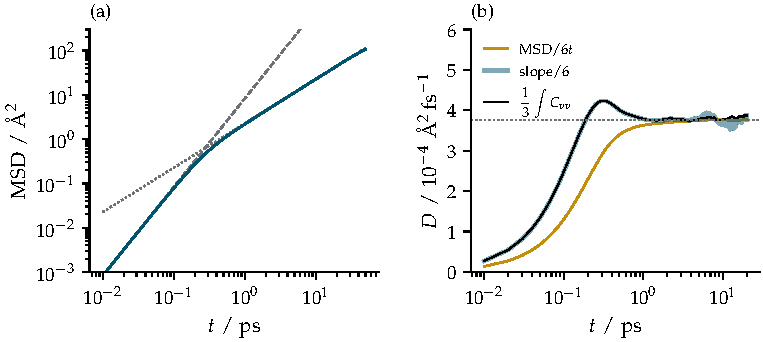
\includegraphics{ch16_observables/msd}
\caption{Liquid argon at fixed energy and \SI{132.1}{\kelvin}
(\SI{100}{\pico\second}, paths summed from velocities saved every
\SI{10}{\femto\second}). (a) The mean squared displacement against time,
with the ballistic $3\kB Tt^2/m$ (dashed) and $6Dt$ (dotted). (b) Three
estimates of $D$ against the time they reach: MSD$/6t$, the slope of the
MSD divided by 6 (thick, pale), and the Green-Kubo integral
$\frac13\int_0^tC_{vv}$ of \cref{sec:ob-vacf} (thin), which coincide; the
dotted line is $D$ from the fit over 2 to \SI{20}{\pico\second}.}
\label{fig:ob-msd}
\end{figure}

\begin{keyidea}
The mean squared displacement grows as $2dDt$ once the motion forgets
its velocity, and as $(3\kB T/m)t^2$ before. $D$ is fitted to its linear
part, from unwrapped paths with the centre of mass removed and averaged
over every starting frame, with its error from blocks and a correction
for the size of the cell.
\end{keyidea}

\notebook{16}{move the fitting window across the MSD of liquid argon}

\begin{selfcheck}
An atom of mass \SI{40}{\amu} in a liquid at \SI{300}{\kelvin} has $D =
\SI{3e-4}{\angstrom\squared\per\femto\second}$. Roughly when does its
motion stop being ballistic?
\end{selfcheck}

%=============================================================================!
% 16.6  VELOCITIES THAT REMEMBER                                              !
%=============================================================================!
\section{Velocities that remember}
\label{sec:ob-vacf}

A walk whose steps are independent spreads as $2dDt$, but an atom's
velocity is not new at each instant: it changes only as collisions turn
it, and for a while each velocity resembles the one before, as the
samples of Chapter~15 resembled their predecessors. The memory of the
velocity sets how far the atom gets, and measuring it gives the diffusion
coefficient by a second route, and other transport coefficients by the
same one.

\subsection*{The velocity autocorrelation function}

The velocity autocorrelation function is
\begin{equation*}
   C_{vv}(t) = \ens{\vb{v}(t_0)\cdot\vb{v}(t_0 + t)} ,
\end{equation*}
averaged over the atoms and over the starting times $t_0$, the
covariance of Chapter~15 for a vector quantity. At $t = 0$ it is
$\ens{v^2} = 3\kB T/m$, and it falls towards zero as collisions scatter
the velocity. In liquid argon (\cref{fig:ob-vacf}a) it reaches zero at
\SI{320}{\femto\second} and goes negative, to $-0.056\,C_{vv}(0)$ at
\SI{420}{\femto\second}: an atom that has run into the cage of its
neighbours rebounds, and its velocity points, on average, backwards. In
the crystal at \SI{21}{\kelvin}, where the cage never opens, it
oscillates, reaching $-0.62\,C_{vv}(0)$ at \SI{330}{\femto\second}, the
atom swinging back and forth about its site. \texttt{velocity\_autocorrelation}
of \texttt{mdlab} computes the average over every pair of frames by the
fast Fourier transform, a tool \cref{sec:ob-fourier} explains.

\subsection*{From the velocity to the displacement}

The displacement is the integral of the velocity, $\vb{r}(t_0 + t) -
\vb{r}(t_0) = \int_0^t\vb{v}(t_0 + t')\,\dd t'$. Its square is a double
integral, and averaging,
\begin{equation*}
   \ens{\lvert\vb{r}(t_0 + t) - \vb{r}(t_0)\rvert^2}
   = \int_0^t\!\!\int_0^t\ens{\vb{v}(t_0 + t')\cdot\vb{v}(t_0 + t'')}
   \,\dd t'\,\dd t''
   = \int_0^t\!\!\int_0^tC_{vv}(t'' - t')\,\dd t'\,\dd t'' ,
\end{equation*}
since in a settled run the average depends only on the separation of the
two times. For the same reason $C_{vv}$ is even: shifting the start from
$t_0$ to $t_0 - t$ turns $\ens{\vb{v}(t_0)\cdot\vb{v}(t_0 - t)}$ into
$\ens{\vb{v}(t_0 - t)\cdot\vb{v}(t_0)}$, so $C_{vv}(-t) = C_{vv}(t)$. The
integrand is constant along the lines $t'' - t' = s$ across the square $0
\le t', t'' \le t$. The line at separation $s$ runs from $(0, s)$ to $(t -
s, t)$, a length $\sqrt2\,(t - s)$, and the line at $s + \dd s$ lies
parallel to it at the distance $\dd s/\sqrt2$, so the strip between them
has the area $(t - s)\,\dd s$; the lines at $-s$ cut out an equal strip.
Collecting the strips,
\begin{equation}
   \ens{\lvert\vb{r}(t_0 + t) - \vb{r}(t_0)\rvert^2}
   = 2\int_0^t(t - s)\,C_{vv}(s)\,\dd s ,
   \label{eq:ob-msd-vacf}
\end{equation}
the same counting of pairs by their separation that gave the variance of
a correlated mean in \cref{eq:cv-var}. Written as $2t\int_0^tC_{vv}\,\dd s -
2\int_0^tsC_{vv}\,\dd s$, it has the slope in $t$
\begin{equation*}
   2\int_0^tC_{vv}(s)\,\dd s + 2tC_{vv}(t) - 2tC_{vv}(t)
   = 2\int_0^tC_{vv}(s)\,\dd s ,
\end{equation*}
by the product rule (\cref{sec:ne-drag}) for the first term and, for
both, the fundamental theorem of calculus, by which the slope of an
integral with respect to its upper limit is the integrand there
(\cref{sec:mo-integrating}). Once
$C_{vv}$ has died away this slope is constant and equals $6D$ by
\cref{eq:ob-einstein}, so
\begin{equation}
   D = \frac13\int_0^\infty C_{vv}(t)\,\dd t ,
   \label{eq:ob-gk}
\end{equation}
a Green-Kubo formula: a transport coefficient as the integral of the
autocorrelation function of a current, here the velocity of one
atom\cite{AllenTildesley2017}.

The two routes are one identity, and on the same run they agree.
\Cref{fig:ob-msd}(b) plots the slope of the MSD divided by 6 and the
running integral $\frac13\int_0^tC_{vv}$, which lie on each other at
every $t$; from 1 to \SI{10}{\pico\second} the integral strays from its
final value by at most 1.2\%. Averaged over 2 to \SI{10}{\pico\second}, it
gives $D = \SI{3.784e-4}{\angstrom\squared\per\femto\second}$, 0.5\% above
the fit to the MSD over 2 to \SI{20}{\pico\second}. The integral
overshoots before it settles, to 1.12 times its final value at
\SI{320}{\femto\second}, where $C_{vv}$ crosses zero, because the
negative part that follows takes back some of what came before: the
rebound from the cage slows diffusion.

\subsection*{The viscosity}

The same form gives the shear viscosity, the friction of one layer of a
liquid sliding over another, as the integral of the autocorrelation
function of the shear stress, the off-diagonal pressure $\mathsf{P}_{xy}$
of \cref{sec:pr-tensor}:
\begin{equation*}
   \eta_{\mathrm s} = \frac{V}{\kB T}\int_0^\infty
   \ens{\mathsf{P}_{xy}(0)\,\mathsf{P}_{xy}(t)}\,\dd t .
\end{equation*}
Its derivation needs the response of a liquid to a slow shear, which
this book does not develop; it is given by Allen and
Tildesley\cite{AllenTildesley2017}. Chapter~15 recorded
$\mathsf{P}_{xy}$, $\mathsf{P}_{xz}$ and $\mathsf{P}_{yz}$ at every step of
twelve runs of liquid argon at 133.7 to \SI{135.3}{\kelvin}, the two of
\SI{2}{\nano\second} and the ten of \SI{1}{\nano\second} at five sizes,
\SI{14}{\nano\second} in all. Each component of each run gives one
estimate, and the integrals, averaged and given the standard error of the
twelve runs, reach 0.98 of their plateau by \SI{1}{\pico\second}
(\cref{fig:ob-vacf}b). Over
1 to \SI{3}{\pico\second},
\begin{equation*}
   \eta_{\mathrm s} = (1.853 \pm 0.038)\times10^{-4}\,\si{\pascal\second} ,
\end{equation*}
or $2.04 \pm 0.04$ in the reduced unit $\sqrt{m\varepsilon}/\sigma^2$.
\Cref{sec:cv-size} inferred $(2.18 \pm 0.20)\times10^{-4}$\,\si{\pascal\second}
from the way $D$ changed with the size of the box through
\cref{eq:cv-yh}, and the two lie 1.6 combined errors apart: the change
of $D$ with size is the return flow of the hydrodynamic theory, to within
its error. With this $\eta_{\mathrm s}$ the correction of \cref{eq:cv-yh}
for 256 atoms is \SI{0.651e-4}{\angstrom\squared\per\femto\second}, which
added to the 256-atom value of \num{3.914e-4} gives \num{4.565e-4},
against the $(4.503 \pm 0.032)\times10^{-4}$ extrapolated from five sizes.

Beyond \SI{3}{\pico\second} the integral wanders: the correlation has
gone, and what is added is noise whose spread grows with the upper limit,
as the integral of a sum of noisy terms does. The integral is read where
it has settled and not later (\cref{sec:ob-trajectory}).

\begin{figure}[htb]
\centering
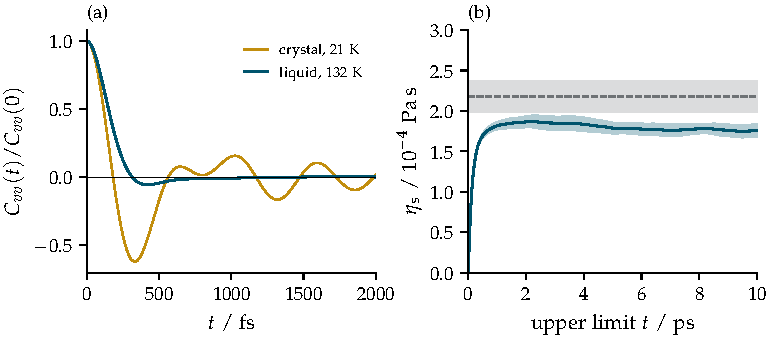
\includegraphics{ch16_observables/vacf}
\caption{(a) The velocity autocorrelation function of liquid argon at
fixed energy and \SI{132}{\kelvin} and of the fcc crystal at
\SI{21}{\kelvin}, each divided by its value at $t = 0$. (b) The
Green-Kubo integral of the shear stress, $(V/\kB T)\int_0^t\ens{
\mathsf{P}_{xy}(0)\mathsf{P}_{xy}(t')}\dd t'$, from the
\SI{14}{\nano\second} of Chapter~15's runs near \SI{135}{\kelvin}, with
twice its standard error over the twelve runs (band), against the
viscosity that \cref{eq:cv-yh} inferred from the change of $D$ with
size (dashed, with its error).}
\label{fig:ob-vacf}
\end{figure}

\begin{keyidea}
The mean squared displacement is twice the integral of the velocity
autocorrelation function weighted by $t - s$, so $D$ is a third of the
integral of $C_{vv}$, a Green-Kubo formula. Both routes give the same $D$
from the same run. The shear viscosity is the same kind of integral of
the shear stress's autocorrelation, read where it has settled.
\end{keyidea}

\notebook{16}{integrate the velocity autocorrelation function and watch it settle}

\begin{selfcheck}
Why does the negative dip of $C_{vv}$ in a liquid make $D$ smaller than
the integral of its first, positive part alone?
\end{selfcheck}

%=============================================================================!
% 16.7  CHARGE TRANSPORT                                                      !
%=============================================================================!
\section{Charge transport}
\label{sec:ob-charge}

An electrolyte carries current through the motion of its ions. If each
ion moved independently, its diffusion coefficient would determine its
contribution to the conductivity. But a cation and an anion that move
together as a neutral pair can diffuse without carrying net charge.
We first derive the independent-ion estimate, then include correlations
and measure their effect in a model molten salt.

\subsection*{Drift against diffusion}

Suppose each ion of some kind feels a steady force $F_x$ along $x$, for
instance from an electric field. Its collisions with its neighbours act,
on average, as a friction that grows with its velocity, so it does not
speed up for ever: it drifts with a mean velocity $v_{\mathrm d}$ in the
direction of the force, at which the friction balances the force, while
diffusion spreads it. The drift and the diffusion are tied together. If
the force comes from a potential energy $U(x)$, so that $F_x = -\dd U/\dd
x$, the ions settle into the canonical density $\rho(x) \propto
\mathrm{e}^{-\beta U(x)}$ (\cref{sec:sm-canonical}), whose slope is
$\dd\rho/\dd x = -\beta\rho\,\dd U/\dd x = \beta F_x\rho$. At equilibrium no
net flow remains, so the drift's flow $\rho\,v_{\mathrm d}$ and Fick's flow
$-D\,\dd\rho/\dd x$ cancel:
\begin{equation*}
   \rho\,v_{\mathrm d} - D\beta F_x\rho = 0 , \qquad
   v_{\mathrm d} = \beta D\,F_x ,
\end{equation*}
the Einstein relation: the drift velocity per unit force is the
diffusion coefficient divided by $\kB T$. The same atom that wanders
fast also drifts fast when pushed.

In an electric field $\mathcal{E}$ along $x$, ion $i$, of charge $q_i$,
feels $F_x = q_i\mathcal{E}$ and drifts at $\beta D_iq_i\mathcal{E}$, with
$D_i$ the diffusion coefficient of its kind. The current density, the
charge carried across unit area in unit time, is the sum over the ions of
each charge times its drift velocity, divided by the volume, $\sum_iq_i
\times \beta D_iq_i\mathcal{E}/V$. Divided by $\mathcal{E}$, this is the
conductivity of independent ions, the Nernst-Einstein value
\begin{equation}
   \sigma_{\mathrm{NE}} = \frac{1}{V\kB T}\sum_iq_i^2D_i ;
   \label{eq:ob-ne}
\end{equation}
cations and anions add, $q_i^2$ being positive for both. In the units of
\texttt{mdlab}, $e^2$ per \si{\angstrom}, \si{\femto\second} and
\si{\electronvolt}, a conductivity of 1 is \SI{1.602e6}{\siemens\per\metre},
the siemens being the ampere per volt.

\subsection*{The conductivity of the whole}

Ions do not move independently. The general result has the form of
\cref{eq:ob-einstein} for the charge displacement $\vb{M}_q(t) =
\sum_iq_i\vb{r}_i(t)$, the sum of every ion's position weighted by its
charge:
\begin{equation}
   \sigma_{\mathrm e} = \frac{1}{6V\kB T}\lim_{t\to\infty}\frac{\dd}{\dd t}
   \ens{\lvert\vb{M}_q(t_0 + t) - \vb{M}_q(t_0)\rvert^2} ,
   \label{eq:ob-sigma}
\end{equation}
whose derivation, like the viscosity's, uses the response of the system
to a weak field\cite{AllenTildesley2017}. Expanding the square shows how
it differs from \cref{eq:ob-ne}. With $\Delta\vb{r}_i$ the displacement of
ion $i$,
\begin{equation*}
   \ens{\lvert\Delta\vb{M}_q\rvert^2}
   = \sum_iq_i^2\ens{\lvert\Delta\vb{r}_i\rvert^2}
   + \sum_i\sum_{j\neq i}q_iq_j\ens{\Delta\vb{r}_i\cdot\Delta\vb{r}_j} .
\end{equation*}
The first sum grows as $\sum_iq_i^2\,6D_it$ and gives
\cref{eq:ob-ne}; the second holds the correlations between different
ions. A cation and an anion that move together have $q_iq_j < 0$ and
$\ens{\Delta\vb{r}_i\cdot\Delta\vb{r}_j} > 0$, a negative term, and lower
the conductivity below $\sigma_{\mathrm{NE}}$. Their ratio is the Haven
ratio $H_{\mathrm R} = \sigma_{\mathrm{NE}}/\sigma_{\mathrm e}$. Like $D$,
$\sigma_{\mathrm e}$ also follows from a Green-Kubo integral, of the
autocorrelation function of the charge current $\sum_iq_i\vb{v}_i$, by
the steps of \cref{eq:ob-msd-vacf}.

\subsection*{A model molten salt}

The test system is 64 ions in a cubic cell of side \SI{13.4}{\angstrom},
32 of charge $+e$ with the mass of sodium and 32 of $-e$ with that of
chlorine. Every pair repels as $A\mathrm{e}^{-r/r_{\mathrm{rep}}}$ with
$r_{\mathrm{rep}} = \SI{0.3}{\angstrom}$, and $A = \SI{6231}{\electronvolt}$ is
set so that a pair of opposite charges has its least energy at
\SI{2.8}{\angstrom}, where the repulsion's slope $A\mathrm{e}^{-r/r_{\mathrm
{rep}}}/r_{\mathrm{rep}}$ balances the
Coulomb pull $k_{\mathrm e}e^2/r^2$; the Coulomb energy is summed by Ewald's
method (\cref{sec:md-ewald}). The model is illustrative, chosen to
resemble an alkali halide, a salt of a metal such as sodium with a
halogen such as chlorine, and is not fitted to sodium chloride. Eight
runs each melt the lattice at \SI{4000}{\kelvin}, hold
\SI{1500}{\kelvin} with CSVR for \SI{40}{\pico\second} and then run
\SI{1}{\nano\second} at fixed energy with steps of \SI{2}{\femto\second}.
Their energies differ, since 64 ions leave the thermostatted stage with an
energy that fluctuates widely, so they sit at temperatures from 1362 to
\SI{1721}{\kelvin}.

The liquid is ordered by charge (\cref{fig:ob-salt}a). Around a cation
the anions crowd at \SI{3.07}{\angstrom}, where $g_{+-}$ rises to 3.65,
and other cations lie farther out, $g_{++}$ peaking at 1.66 at
\SI{4.37}{\angstrom}, $g_{--}$ alike at \SI{4.32}{\angstrom}; each cation
has 6.76 anions out to the first minimum of $g_{+-}$, at
\SI{4.87}{\angstrom}.

Each run gives $\sigma_{\mathrm e}$ from \cref{eq:ob-sigma}, with the
charge displacement recorded at every step and fitted over 1 to
\SI{5}{\pico\second}, and $\sigma_{\mathrm{NE}}$ from the two kinds' $D$
over the same window. The Green-Kubo route agrees with the displacement
in every run to within 0.6\%. Both conductivities rise with the run's
temperature (\cref{fig:ob-salt}b), and the Nernst-Einstein value lies
above the true one by more than half a percent in six runs of eight,
within it in one and below it in one. Over the eight, at $(1487 \pm
45)$\,\si{\kelvin}, $\sigma_{\mathrm e} = (158 \pm 9)$\,\si{\siemens\per
\metre} and $\sigma_{\mathrm{NE}} = (168 \pm 10)$\,\si{\siemens\per\metre},
errors that come mostly from the spread of the runs' temperatures. Their
ratio, taken run by run, shows no trend with the temperature in the
figure, and averages
\begin{equation*}
   H_{\mathrm R} = 1.062 \pm 0.022 ,
\end{equation*}
2.8 errors above 1, beyond the 2.365 that Student's factor for eight
runs, seven degrees of freedom, sets at 95\% (\cref{sec:cv-mean}): the
ions' motions are correlated, and treating them as independent
overstates the conductivity of this melt by about 6\%. The diffusion
coefficients of the two kinds over the eight runs, $(5.19 \pm 0.46)$ and
$(5.03 \pm 0.45)\times10^{-4}$\,\si{\angstrom\squared\per\femto\second}
for the cations and the anions, are the same within errors that again
reflect the temperatures; taken run by run, which removes the
temperature, their ratio is $1.033 \pm 0.008$, the cations faster in
seven runs of eight.

\begin{figure}[htb]
\centering
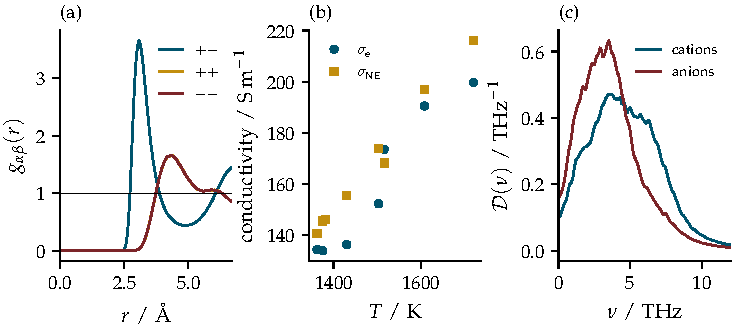
\includegraphics{ch16_observables/salt}
\caption{The model molten salt, 64 ions in eight runs of
\SI{1}{\nano\second} at fixed energy. (a) The partial radial distribution
functions $g_{+-}$, $g_{++}$ and $g_{--}$. (b) The conductivity of each
run from the charge displacement (circles) and from Nernst-Einstein with
the ions' own diffusion coefficients (squares), against the run's
temperature. (c) The vibrational density of states of the cations and of
the anions in the first run (\cref{sec:ob-vdos}).}
\label{fig:ob-salt}
\end{figure}

\begin{keyidea}
An ion pushed by a force $F_x$ drifts at $\beta DF_x$, so independent ions
conduct as $\sigma_{\mathrm{NE}} = \sum_iq_i^2D_i/V\kB T$. The true
conductivity comes from the mean squared displacement of the total charge
displacement $\sum_iq_i\vb{r}_i$, whose cross terms hold the correlations
between ions; the Haven ratio $\sigma_{\mathrm{NE}}/\sigma_{\mathrm e}$
measures them.
\end{keyidea}

\notebook{16}{compare the charge displacement with the ions' own displacements}

\begin{selfcheck}
If every cation were permanently bound to one anion, moving as a neutral
pair, what would $\sigma_{\mathrm e}$ be, and what would
$\sigma_{\mathrm{NE}}$ still give?
\end{selfcheck}

%=============================================================================!
% 16.8  DIFFUSION IN LAYERS                                                   !
%=============================================================================!
\section{Diffusion in layers}
\label{sec:ob-layers}

Lithium in graphite can move between the carbon sheets much more readily
than it can cross them. A single diffusion coefficient hides this
difference: we need the mean squared displacement in each direction.
After measuring it in the layered model solid, we connect diffusion to
hops between lattice sites and test the assumption that successive hops
are independent.

\subsection*{The diffusion tensor}

The MSD of \cref{eq:ob-einstein} is the sum of three parts, $\ens{\Delta
x^2} + \ens{\Delta y^2} + \ens{\Delta z^2}$, and each grows as $2D_{xx}t$,
$2D_{yy}t$ and $2D_{zz}t$ with its own coefficient. More generally the
products of the components define the diffusion tensor, $\ens{\Delta
r_\alpha\Delta r_\beta} \to 2D_{\alpha\beta}t$, a symmetric $3\times3$
matrix whose eigenvectors are the directions in which the spreading is
fastest and slowest (\cref{sec:os-modes}). In a layered solid with its
sheets at right angles to $z$, symmetry makes $z$ one of them and leaves
the two in the plane equal, $D_{xx} = D_{yy}$, and the diffusion
coefficient that a single number would give, a third of the trace,
mixes two very different motions.

\Cref{sec:pr-shape} built a model of such a solid: triangular sheets, each
bound strongly within itself and weakly to its neighbours, with 108 guest
atoms of lithium's mass grown into the hollows between them. Held at
\SI{150}{\kelvin} by CSVR in its relaxed cell for \SI{500}{\pico\second},
its guests' MSD along each axis, measured from the centre of mass, gives
from five blocks of \SI{100}{\pico\second} and fits over 5 to
\SI{50}{\pico\second}
\begin{equation*}
   D_{xx} = (1.16 \pm 0.11)\times10^{-4}\,\si{\angstrom\squared\per
   \femto\second} , \qquad
   D_{yy} = (1.02 \pm 0.05)\times10^{-4}\,\si{\angstrom\squared\per
   \femto\second} .
\end{equation*}
The two in the plane agree within their errors. Along $z$ the MSD is
\SI{0.113}{\angstrom\squared} at \SI{1}{\pico\second},
\SI{0.126}{\angstrom\squared} at 10 and \SI{0.132}{\angstrom\squared} at
\SI{50}{\pico\second} (\cref{fig:ob-layers}a), and no guest moves more
than \SI{1.73}{\angstrom} along $z$ in the whole run: the guests rattle
between their two sheets, and none crosses to the next gap,
\SI{3.40}{\angstrom} away. A single crossing would add
\SI{11.6}{\angstrom\squared} to one guest's square, and so
$\SI{11.6}{\angstrom\squared}/108$ to the mean, and one in the
\SI{500}{\pico\second} would have meant $D_{zz} \approx
\SI{1.1e-7}{\angstrom\squared\per\femto\second}$. This is the scale of one detectable crossing, not a statistical upper
bound on $D_{zz}$: a finite run can miss a rare event. It is a thousand
times smaller than the in-plane value. A straight line fitted to the
levelling MSD would only measure its slow approach to the plateau;
\cref{ex:ip-rate} shows how zero events give a confidence bound.

\subsection*{Hops between sites}

On the model surface of \cref{sec:en-surface} a lithium atom moves by
hops between hollows a distance $a = \SI{2.46}{\angstrom}$ apart, and
Chapter~13 counted them. If each hop goes to one of the six neighbouring
hollows at random, independently of the last, the atom performs the
random walk of \cref{sec:ob-msd} with steps of length $a$, and after $n$
hops its mean squared displacement is $na^2$. At a rate of $k_{\mathrm h}$ hops
per unit time, $n = k_{\mathrm h}t$, and comparing $k_{\mathrm h}ta^2$ with $2dDt$ for
$d = 2$,
\begin{equation*}
   D = \frac{k_{\mathrm h}a^2}{4} .
\end{equation*}
Counted hops thus give a diffusion coefficient without fitting an MSD,
and a count has the error bar of \cref{sec:ob-reactions}, $\sqrt n$. If
the hops have various lengths $\ell$ but still forget their direction,
the same sum gives $n\ens{\ell^2}$ after $n$ hops, and $D = k_{\mathrm
h}\ens{\ell^2}/4$.

The relation assumes that hops forget their direction. At
\SI{1000}{\kelvin}, with Langevin friction of \SI{1}{\per\pico\second}, 1000
atoms over \SI{200}{\pico\second} make \num{179680} hops, a rate of $k_{\mathrm h}
= (0.8984 \pm 0.0021)$ per atom and picosecond, Chapter~13's rate again;
$k_{\mathrm h}a^2/4$ is then \SI{13.6e-4}{\angstrom\squared\per\femto\second},
but the MSD over 2 to \SI{10}{\pico\second} gives $D =
\SI{92.3e-4}{\angstrom\squared\per\femto\second}$, 6.79 times more. The
ratio $f = 4D/k_{\mathrm h}a^2$, the correlation factor, exceeds 1 for two
reasons. An atom with enough energy to cross a bridge often keeps it long
enough to cross the next before the friction takes it away, so that 17\%
of the counted hops, from one hollow where the atom is seen to the next,
are longer than $a$, and their mean square is $1.96a^2$. And successive
hops tend to keep their direction: $4D/k_{\mathrm h}\ens{\ell^2}$, which would
be 1 for hops that forget it, is 3.46. Raising the friction to 3, 10 and
\SI{30}{\per\pico\second} drains the energy faster: $f$ falls to 3.24,
1.63 and 1.13, as the product of $\ens{\ell^2}/a^2$, 1.66, 1.29 and 1.07,
and the memory of direction, 1.96, 1.27 and 1.05 (\cref{fig:ob-layers}b),
while $k_{\mathrm h}$ stays near 0.90 until the highest friction, which slows
the hops themselves to 0.708 per picosecond, as Chapter~13 found. How large $f$ is in a real crystal
depends on how fast the lattice takes away an arriving atom's energy,
which only a measurement of both $D$ and $k_{\mathrm h}$ settles.

\begin{figure}[htb]
\centering
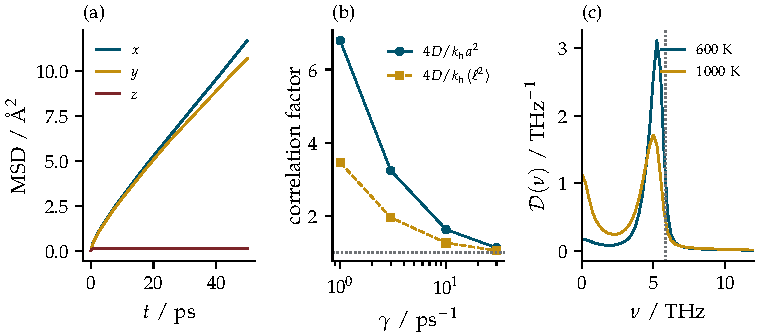
\includegraphics{ch16_observables/layers}
\caption{(a) The guests of the layered model solid at \SI{150}{\kelvin}:
their mean squared displacement along $x$, $y$ and $z$, measured from the
centre of mass. (b) Lithium on the model surface at \SI{1000}{\kelvin}:
the correlation factor $f = 4D/k_{\mathrm h}a^2$, with $D$ from the MSD and
$k_{\mathrm h}$ from counted hops (circles), and $4D/k_{\mathrm h}\ens{\ell^2}$,
with $\ens{\ell^2}$ the mean square length of a counted hop (squares),
against the Langevin friction. (c) The
vibrational density of states of the lithium atoms at 600 and
\SI{1000}{\kelvin} (friction \SI{1}{\per\pico\second}), with the
frequency of small vibrations in a hollow (dotted; \cref{sec:ob-vdos}).}
\label{fig:ob-layers}
\end{figure}

\begin{keyidea}
In an anisotropic solid the MSD is taken along each direction, giving the
diffusion tensor; in a layered solid the motion along the layers and
across them differ by orders of magnitude. Diffusion by hops between
sites a distance $a$ apart gives $D = fk_{\mathrm h}a^2/4$ in two dimensions,
with $f = 1$ when successive hops are independent and one site long, and
$f > 1$ when they carry the atom past the next site or keep their
direction.
\end{keyidea}

\notebook{16}{split the MSD of the guests into its three directions}

\begin{selfcheck}
On a simple cubic lattice of spacing $a$ in three dimensions, with
independent hops at a total rate $k_{\mathrm h}$, what is $D$?
\end{selfcheck}

%=============================================================================!
% 16.9  FREQUENCIES IN A SIGNAL                                               !
%=============================================================================!
\section{Frequencies in a signal}
\label{sec:ob-fourier}

A chord struck on a piano reaches the ear as one wobbling pressure, yet a
listener hears two notes, and a tuner's display shows two peaks at their
pitches. Something takes a signal in time apart into the frequencies it
holds. The same operation turns the velocities of a run into the
frequencies its atoms vibrate at, and it has been used twice already
without explanation, to compute correlation functions quickly in
Chapter~15 and in \cref{sec:ob-vacf}. This section supplies it: complex
numbers, the Fourier transform, its discrete form, the fast algorithm,
and what sampling a signal at intervals does to the frequencies one can
see.

\begin{toolbox}[Complex numbers and Euler's formula]
A complex number $z = x + \mathrm{i}y$ is a pair of real numbers $x$ and
$y$ combined with a symbol $\mathrm{i}$ whose square is $-1$. They add and
multiply as ordinary numbers do, replacing $\mathrm{i}^2$ by $-1$
wherever it appears: $(a + \mathrm{i}b)(c + \mathrm{i}d) = ac - bd +
\mathrm{i}(ad + bc)$. Drawn as the point $(x, y)$, $z$ is an arrow from
the origin; its length is $\lvert z\rvert = \sqrt{x^2 + y^2}$, and with
the conjugate $\bar z = x - \mathrm{i}y$, $z\bar z = x^2 + y^2 = \lvert z
\rvert^2$. The Taylor series of \cref{sec:mo-taylor} for $\mathrm{e}^x$,
$\cos x$ and $\sin x$ are
\begin{equation*}
   \mathrm{e}^x = \sum_{n\ge0}\frac{x^n}{n!} , \quad
   \cos x = 1 - \frac{x^2}{2!} + \frac{x^4}{4!} - \cdots , \quad
   \sin x = x - \frac{x^3}{3!} + \frac{x^5}{5!} - \cdots .
\end{equation*}
Putting $x = \mathrm{i}\theta$ in the first, the even powers
$(\mathrm{i}\theta)^{2m} = (-1)^m\theta^{2m}$ give the series of $\cos\theta$
and the odd powers $(\mathrm{i}\theta)^{2m+1} = \mathrm{i}(-1)^m
\theta^{2m+1}$ give $\mathrm{i}$ times that of $\sin\theta$:
\begin{equation*}
   \mathrm{e}^{\mathrm{i}\theta} = \cos\theta + \mathrm{i}\sin\theta ,
\end{equation*}
Euler's formula, an arrow of length 1 at the angle $\theta$. With
$-\theta$ in place of $\theta$ it gives $\mathrm{e}^{-\mathrm{i}\theta} =
\cos\theta - \mathrm{i}\sin\theta$, and adding and subtracting the two,
\begin{equation*}
   \cos\theta = \frac{\mathrm{e}^{\mathrm{i}\theta} +
   \mathrm{e}^{-\mathrm{i}\theta}}{2} , \qquad
   \sin\theta = \frac{\mathrm{e}^{\mathrm{i}\theta} -
   \mathrm{e}^{-\mathrm{i}\theta}}{2\mathrm{i}} ,
\end{equation*}
so any cosine or sine is a sum of two such exponentials. Exponentials
multiply by adding their powers, $\mathrm{e}^a\mathrm{e}^b = \mathrm{e}^{a
+ b}$, for complex numbers as for real ones: multiplying the two series
and collecting the terms of total power $n$ gives $\sum_{l}a^lb^{n -
l}/l!(n - l)! = (a + b)^n/n!$ by the binomial expansion, which uses only
the rules of adding and multiplying. So $\mathrm{e}^{\mathrm{i}A}
\mathrm{e}^{\mathrm{i}B} = \mathrm{e}^{\mathrm{i}(A + B)}$, which written
out is the pair of addition formulae of \cref{eq:mo-addition}: turning by
$A$ and then by $B$ turns by $A + B$. In this language the sums of
\cref{eq:ob-sq} are the real and imaginary parts of one sum, $\mathcal{C}
+ \mathrm{i}\mathcal{S} = \sum_j\mathrm{e}^{\mathrm{i}\vb{G}\cdot\vb{r}_j}$,
and $S(\vb{G})$ is its squared length over $N$.
\end{toolbox}

\subsection*{The Fourier transform}

A signal $x(t)$ that repeats with period $t_{\mathrm p}$ is a sum of
cosines and sines that repeat with it (\cref{sec:md-ewald}), which by the
toolbox are sums of $\mathrm{e}^{2\pi\mathrm{i}mt/t_{\mathrm p}}$ for whole
numbers $m$, positive and negative, each at the frequency $m/t_{\mathrm
p}$:
\begin{equation*}
   x(t) = \sum_mc_m\,\mathrm{e}^{2\pi\mathrm{i}mt/t_{\mathrm p}} , \qquad
   c_m = \frac{1}{t_{\mathrm p}}\int_{-t_{\mathrm p}/2}^{t_{\mathrm p}/2}
   x(t)\,\mathrm{e}^{-2\pi\mathrm{i}mt/t_{\mathrm p}}\,\dd t ,
\end{equation*}
the coefficients found, as in Chapter~10, because the average of
$\mathrm{e}^{2\pi\mathrm{i}(m - m')t/t_{\mathrm p}}$ over a period is 1 for
$m = m'$ and 0 otherwise. A signal that does not repeat is the limit of a
long period. The frequencies $\nu_m = m/t_{\mathrm p}$ then lie a small
distance $\Delta\nu = 1/t_{\mathrm p}$ apart, and with $\hat x(\nu_m) =
t_{\mathrm p}c_m$ the series reads $x(t) = \sum_m\hat x(\nu_m)\,
\mathrm{e}^{2\pi\mathrm{i}\nu_mt}\,\Delta\nu$, a sum of thin strips that
becomes an integral over $\nu$ as $\Delta\nu$ shrinks
(\cref{sec:mo-integrating}), while the integral for $\hat x(\nu_m)$ comes
to cover all times:
\begin{equation}
   \hat x(\nu) = \int_{-\infty}^{\infty}x(t)\,\mathrm{e}^{-2\pi\mathrm{i}
   \nu t}\,\dd t , \qquad
   x(t) = \int_{-\infty}^{\infty}\hat x(\nu)\,\mathrm{e}^{2\pi\mathrm{i}
   \nu t}\,\dd\nu ,
   \label{eq:ob-ft}
\end{equation}
the Fourier transform and its inverse. $\hat x(\nu)$ is a complex number
for each frequency, whose length says how much of that frequency the
signal holds and whose angle gives the wave's phase. A signal observed
for a time $t_{\mathrm f}$ cannot separate frequencies closer than about $1/t_{\mathrm f}$, since
two waves that differ by less than that drift apart by less than a whole
cycle over the record: a chord recorded for \SI{50}{\milli\second} shows
its notes only if they differ by more than \SI{20}{\hertz}.

\subsection*{The discrete Fourier transform}

A run records a signal at $N_{\mathrm s}$ equally spaced times $t_n =
n\Dt$, $n = 0, \dots, N_{\mathrm s} - 1$, and the integral becomes a sum,
\begin{equation}
   X_k = \sum_{n=0}^{N_{\mathrm s}-1}x_n\,
   \mathrm{e}^{-2\pi\mathrm{i}kn/N_{\mathrm s}} , \qquad
   x_n = \frac{1}{N_{\mathrm s}}\sum_{k=0}^{N_{\mathrm s}-1}X_k\,
   \mathrm{e}^{2\pi\mathrm{i}kn/N_{\mathrm s}} ,
   \label{eq:ob-dft}
\end{equation}
the discrete Fourier transform, $X_k$ belonging to the frequency $\nu_k =
k/N_{\mathrm s}\Dt$. The inverse holds because of a geometric sum.
Putting the first sum, with the index $n'$, into the second gives
$\frac{1}{N_{\mathrm s}}\sum_{n'}x_{n'}\sum_kw^k$ with $w =
\mathrm{e}^{2\pi\mathrm{i}(n - n')/N_{\mathrm s}}$, and $\sum_{k=0}^{N_{\mathrm
s}-1}w^k = (1 - w^{N_{\mathrm s}})/(1 - w)$, where $w^{N_{\mathrm s}} =
\mathrm{e}^{2\pi\mathrm{i}(n - n')} = 1$; so the sum over $k$ is 0 unless
$w = 1$, that is $n' = n$, when it is $N_{\mathrm s}$, and what remains is
$x_n$. For a real signal, changing $k$ to $N_{\mathrm s} - k$ only turns
each $\mathrm{e}^{-2\pi\mathrm{i}kn/N_{\mathrm s}}$ the other way, so
$X_{N_{\mathrm s}-k} = \bar X_k$: the upper half of the transform mirrors
the lower and belongs to the negative frequencies, and a cosine of height
1 puts $N_{\mathrm s}/2$ at each of its two places. Summed directly,
\cref{eq:ob-dft} needs $N_{\mathrm s}$ products for each of the
$N_{\mathrm s}$ values of $k$, $N_{\mathrm s}^2$ in all; the function
\texttt{dft} of \texttt{mdlab.analysis.spectra} does this.
\Cref{fig:ob-fourier}(a) shows $2\lvert X_k\rvert/400$, which is the
height of each wave, for the notes A (\SI{440}{\hertz}) and E
(\SI{659.25}{\hertz}) of height 1, sampled 8000 times a second for
\SI{50}{\milli\second}. The 400 samples are padded with zeros to 512, the
power of 2 that the fast transform below needs, whose grid of $8000/512 =
\SI{15.6}{\hertz}$ puts the two peaks at the frequencies nearest the
notes, 437.5 and \SI{656.25}{\hertz}.

\subsection*{The fast Fourier transform}

The sum splits into its even and odd samples, $n = 2p$ and $n = 2p + 1$:
\begin{equation*}
   X_k = \sum_{p=0}^{N_{\mathrm s}/2-1}x_{2p}\,\mathrm{e}^{-2\pi\mathrm{i}kp/(N_{\mathrm s}/2)}
   + \mathrm{e}^{-2\pi\mathrm{i}k/N_{\mathrm s}}\sum_{p=0}^{N_{\mathrm s}/2-1}x_{2p+1}\,
   \mathrm{e}^{-2\pi\mathrm{i}kp/(N_{\mathrm s}/2)}
   = X^{\mathrm e}_k + \mathrm{e}^{-2\pi\mathrm{i}k/N_{\mathrm s}}
   X^{\mathrm o}_k ,
\end{equation*}
with $X^{\mathrm e}$ and $X^{\mathrm o}$ the transforms of the even and the
odd samples, each of length $N_{\mathrm s}/2$. These repeat after $N_{\mathrm s}/2$ values of $k$,
and $\mathrm{e}^{-2\pi\mathrm{i}(k + N_{\mathrm s}/2)/N_{\mathrm s}} =
-\mathrm{e}^{-2\pi\mathrm{i}k/N_{\mathrm s}}$, so for $k < N_{\mathrm s}/2$
\begin{equation*}
   X_k = X^{\mathrm e}_k + \mathrm{e}^{-2\pi\mathrm{i}k/N_{\mathrm s}}
   X^{\mathrm o}_k , \qquad
   X_{k+N_{\mathrm s}/2} = X^{\mathrm e}_k - \mathrm{e}^{-2\pi\mathrm{i}k/N_{\mathrm s}}
   X^{\mathrm o}_k :
\end{equation*}
two transforms of half the length and $N_{\mathrm s}$ further operations
give the whole. When $N_{\mathrm s}$ is a power of 2 the halving repeats
down to transforms of one sample, each its own transform, and the work
$W(N_{\mathrm s}) = 2W(N_{\mathrm s}/2) + N_{\mathrm s}$ adds $N_{\mathrm s}$
at each of $\log_2N_{\mathrm s}$ levels, $N_{\mathrm s}\log_2N_{\mathrm s}$
in all. This is the fast
Fourier transform of Cooley and Tukey\cite{CooleyTukey1965}, the one
Chapter~10 promised for particle mesh Ewald. In \texttt{mdlab}:

\begin{code}
def fft(x: ArrayLike) -> NDArray:
    x = np.asarray(x, dtype=complex)
    n = len(x)
    if n == 1:
        return x
    if n % 2:
        raise ValueError("the length must be a power of 2")
    even, odd = fft(x[0::2]), fft(x[1::2])
    twiddle = np.exp(-2j * np.pi * np.arange(n // 2) / n) * odd
    return np.concatenate([even + twiddle, even - twiddle])
\end{code}

\noindent \texttt{dft} and \texttt{fft} agree with NumPy's FFT to
\num{4e-12} and \num{6e-14} on 256 samples. From $N_{\mathrm s} = 64$ to
4096, in three timings on the same machine, the direct sum takes about two
thousand times as long, half the 4096 by which $N_{\mathrm s}^2$ grows,
since a fixed cost of each call weighs most at small $N_{\mathrm s}$; the
recursive \texttt{fft} about 65 times, half the 128 of $N_{\mathrm
s}\log_2N_{\mathrm s}$, for the same reason; and NumPy's compiled FFT
about 10 times (\cref{fig:ob-fourier}c). Every later spectrum uses NumPy's.

\subsection*{Sampling and aliasing}

Samples taken every $\Dt$ cannot tell the frequency $\nu$ from $1/\Dt
- \nu$: at $t_n = n\Dt$,
\begin{equation*}
   \cos\bigl(2\pi(1/\Dt - \nu)n\Dt\bigr) = \cos(2\pi n - 2\pi\nu n
   \Dt) = \cos(2\pi\nu n\Dt) ,
\end{equation*}
since a whole number of turns changes no cosine (the sine changes sign).
The highest frequency that samples can show without confusion is half the
sampling rate, $\nu_{\mathrm N} = 1/2\Dt$, the Nyquist frequency; a
higher one appears folded back below it, at its alias. Films show this
when the spokes of a turning wheel seem to rotate slowly backwards. The E
of the chord, sampled 1000 times a second, gives samples that lie equally
on a wave of $1000 - 659.25 = \SI{340.75}{\hertz}$ (\cref{fig:ob-fourier}b),
to \num{1e-15}. For a run the consequence is direct: frames saved every
$\Dt$ cannot show vibrations faster than $1/2\Dt$, and a vibration
faster than that appears at a false frequency.

\subsection*{Correlation functions by the transform}

The products of \cref{eq:ob-dft} also compute correlations. For real
records $x$ and $y$, the conjugate of the transform of $x$ is $\bar X_k =
\sum_nx_n\mathrm{e}^{2\pi\mathrm{i}kn/N_{\mathrm s}}$, and
\begin{equation*}
   \frac{1}{N_{\mathrm s}}\sum_k\bar X_kY_k\,
   \mathrm{e}^{2\pi\mathrm{i}kj/N_{\mathrm s}}
   = \sum_n\sum_mx_ny_m\,\frac{1}{N_{\mathrm s}}\sum_k
   \mathrm{e}^{2\pi\mathrm{i}k(n + j - m)/N_{\mathrm s}}
   = \sum_nx_ny_{n+j} ,
\end{equation*}
since by the same geometric sum the inner sum is 1 when $m = n + j$ and 0
otherwise, with $n + j$ taken round the end of the record, as if the
record repeated. Padding each record with $N_{\mathrm s}$ zeros first makes
the wrapped products zero, leaving the sum over the $N_{\mathrm s} - j$
true pairs at the lag $j$; dividing by $N_{\mathrm s} - j$ gives the
average. Three transforms of length $2N_{\mathrm s}$ then do the work of
the $N_{\mathrm s}^2/2$ products of every pair. \texttt{stats.autocorrelation} of Chapter~15 and
\texttt{transport.correlation} of this chapter work this way.

\begin{figure}[htb]
\centering
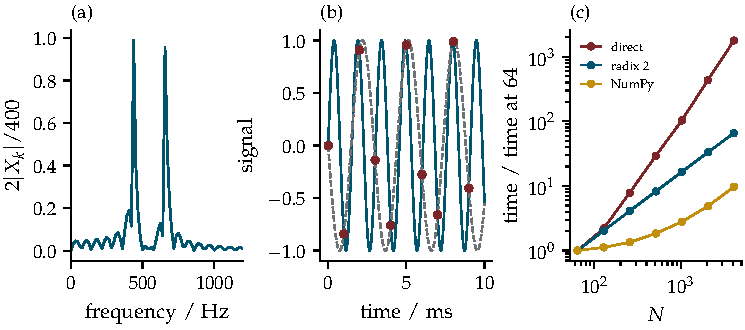
\includegraphics{ch16_observables/fourier}
\caption{(a) The notes A (\SI{440}{\hertz}) and E (\SI{659.25}{\hertz})
of equal strength, sampled 8000 times a second for
\SI{50}{\milli\second} and padded to 512 samples: $2\lvert X_k\rvert/400$,
the height of each wave, against the frequency. (b) The E alone (line) sampled 1000 times a
second (points): the samples lie on a wave of \SI{340.75}{\hertz} as well
(dashed), its alias. (c) The time taken by the direct sum, by the
recursive radix-2 \texttt{fft} and by NumPy's FFT against the number of
samples, each relative to its own time at $N_{\mathrm s} = 64$, the least
of five tries.}
\label{fig:ob-fourier}
\end{figure}

\begin{keyidea}
The Fourier transform writes a signal as waves $\mathrm{e}^{2\pi\mathrm{i}
\nu t}$; a record of length $t_{\mathrm f}$ resolves frequencies about $1/t_{\mathrm f}$ apart.
The discrete transform of $N_{\mathrm s}$ samples costs $N_{\mathrm s}^2$
summed directly and $N_{\mathrm s}\log_2N_{\mathrm s}$ by halving, the fast
Fourier transform. Samples every $\Dt$
show frequencies only up to $1/2\Dt$, and fold higher ones back below
it. Correlation functions are computed through transforms of records
padded with zeros.
\end{keyidea}

\notebook{16}{sample a note and watch it fold back past the Nyquist frequency}

\begin{selfcheck}
A vibration of \SI{30}{\tera\hertz} is recorded with frames every
\SI{20}{\femto\second}. Where does it appear in the spectrum of the frames?
\end{selfcheck}

%=============================================================================!
% 16.10  THE VIBRATIONAL DENSITY OF STATES                                    !
%=============================================================================!
\section{The vibrational density of states}
\label{sec:ob-vdos}

Infrared and neutron spectra report, each weighting the atoms in its own
way, at which frequencies the atoms of a material move, and so does a
trajectory: an atom's velocity, taken apart
into frequencies, says how much of its motion happens at each. Summed
over the atoms this is the vibrational density of states, the spectrum
by which a learned model of motion is first compared with the simulation
it learned from\cite{Thiemann2026}.

\subsection*{The power spectrum of a signal}

For a signal $x(t)$ recorded over a long time $t_{\mathrm f}$, the power at the
frequency $\nu$ is $\lvert\hat x(\nu)\rvert^2/t_{\mathrm f}$, with $\hat x$ the
transform of \cref{eq:ob-ft} over the record. Writing the squared length
as the transform times its conjugate,
\begin{equation*}
   \lvert\hat x(\nu)\rvert^2 = \int_0^{t_{\mathrm f}}\!\!\int_0^{t_{\mathrm f}}x(t)\,x(t')\,
   \mathrm{e}^{-2\pi\mathrm{i}\nu(t - t')}\,\dd t\,\dd t' ,
\end{equation*}
and averaging over many such records turns $x(t)x(t')$ into the
autocorrelation function $C(t - t')$, which in a settled signal depends on
the separation alone. Counting the pairs of times by their separation
$s$, as for \cref{eq:ob-msd-vacf}, each $s$ occurs over a length $t_{\mathrm f} -
\lvert s\rvert$, so
\begin{equation*}
   \frac{\ens{\lvert\hat x(\nu)\rvert^2}}{t_{\mathrm f}} = \int_{-t_{\mathrm f}}^{t_{\mathrm f}}\Bigl(1 -
   \frac{\lvert s\rvert}{t_{\mathrm f}}\Bigr)C(s)\,\mathrm{e}^{-2\pi\mathrm{i}\nu s}\,
   \dd s \to \int_{-\infty}^{\infty}C(s)\,\mathrm{e}^{-2\pi\mathrm{i}\nu s}
   \,\dd s
\end{equation*}
once $t_{\mathrm f}$ is long against the time over which $C$ dies away. The power
spectrum is the Fourier transform of the autocorrelation function, the
theorem of Wiener and Khinchin. Since $C$ is even, the imaginary part of
$\mathrm{e}^{-2\pi\mathrm{i}\nu s}$ cancels between $s$ and $-s$, leaving
$2\int_0^\infty C(s)\cos(2\pi\nu s)\,\dd s$.

\subsection*{The density of states}

Applied to the mass-weighted velocity autocorrelation function per atom,
$C_m(t) = \ens{m\vb{v}(t_0)\cdot\vb{v}(t_0 + t)}$, the theorem gives the
vibrational density of states, scaled so that its area counts the three
directions of each atom:
\begin{equation}
   \mathcal{D}(\nu) = \frac{4}{\kB T}\int_0^\infty C_m(t)\cos(2\pi\nu t)\,
   \dd t , \qquad \int_0^\infty\mathcal{D}(\nu)\,\dd\nu = 3 .
   \label{eq:ob-vdos}
\end{equation}
With $\hat C_m(\nu) = 2\int_0^\infty C_m(t)\cos(2\pi\nu t)\,\dd t$ the
transform of $C_m$, even in $\nu$, $\mathcal{D} = 2\hat C_m/\kB T$, and the
area follows from the inverse transform at $t = 0$: $C_m(0) =
\int_{-\infty}^\infty\hat C_m\,\dd\nu = 2\int_0^\infty\hat C_m\,\dd\nu$, so
the area of $\mathcal{D}$ is $C_m(0)/\kB T$, and $C_m(0) = \ens{mv^2} =
3\kB T$ by equipartition. For a harmonic solid the motion is a sum of
normal modes (\cref{sec:os-modes}), each oscillating at its own
frequency $\nu_k$ with the energy $\kB T$ on average. Each mode adds
$\kB T\cos(2\pi\nu_kt)/N$ to $C_m$ per atom, a spike of area $1/N$ in
$\mathcal{D}$ at $\nu_k$, so $\mathcal{D}$ is the histogram of the mode
frequencies, $3N$ spikes for $N$ atoms making the area 3: the classical
density of states. In a liquid, atoms that wander contribute at zero
frequency, where \cref{eq:ob-vdos} and \cref{eq:ob-gk} give
\begin{equation*}
   \mathcal{D}(0) = \frac{4}{\kB T}\int_0^\infty C_m(t)\,\dd t =
   \frac{12\,mD}{\kB T} ,
\end{equation*}
so the density of states holds the diffusion coefficient too.

A run gives $C_m$ only out to some lag $t_{\mathrm c}$, and cutting the
integral off sharply there adds ripples to $\mathcal{D}$, as cutting
$g(r)$ at half the cell did to $S(G)$ in \cref{sec:ob-sq}.
\texttt{spectra.vdos} multiplies $C_m$ by the window $\cos^2(\pi t/
2t_{\mathrm c})$, which falls smoothly from 1 to 0, transforms it by the
discrete transform of a record extended to negative times, and scales the
result to the area 3. The window blurs each peak over about
$1/t_{\mathrm c}$; a longer $t_{\mathrm c}$ sharpens the peaks and needs a
longer run to keep the noise down.

\subsection*{A crystal, with and without friction}

The fcc crystal at \SI{21}{\kelvin}, \SI{50}{\pico\second} at fixed energy
with velocities every \SI{10}{\femto\second} and $C_m$ taken to
\SI{10}{\pico\second}, has peaks at 0.50, 0.75, 0.95, 1.15, 1.40 and
\SI{1.90}{\tera\hertz} (\cref{fig:ob-vdos}a). Its exact harmonic
frequencies come from the Hessian of the same 256-atom cell
(\cref{sec:os-modes}), by finite differences of the forces: three zero
eigenvalues, the translations of the whole cell, and 765 modes up to
\SI{1.991}{\tera\hertz}. A finite cell has a few distinct frequencies,
and their bare histogram has spikes that the run's windowed spectrum
cannot show, so the fair comparison passes the modes' own $C_m(t) \propto
\sum_k\cos(2\pi\nu_kt)$ through the same window and transform. The overlap
of the two spectra is 0.839 by the score defined below. They agree in
the positions of the peaks, but the run's tallest peak is 3.74 per
terahertz against the modes' 4.28, and the run puts 0.192 of its area of
3 above the highest harmonic frequency, against 0.011 for the modes
through the same window: the run's motion is not exactly harmonic. These
overlaps are taken below \SI{3}{\tera\hertz}, where the crystal's
spectrum lies.

Friction widens every peak, as Chapter~4 found for the response of a
driven spring. A mode
of angular frequency $\omega_0$ damped by Langevin friction $\gamma$ swings
at $\omega_{\mathrm d} = \sqrt{\omega_0^2 - \gamma^2/4}$ (\cref{sec:os-damped}),
and when the friction is small against $\omega_0$ its velocity correlation
decays as $\mathrm{e}^{-\gamma\lvert t\rvert/2}\cos\omega_{\mathrm d}t$, with a
term in $\sin\omega_{\mathrm d}t$ of relative size $\gamma/2\omega_{\mathrm d}$
left out; at the crystal's lowest peak, \SI{0.5}{\tera\hertz}, that size
is 0.32, so the form is rough there. Each half of the cosine,
$\frac12\mathrm{e}^{\pm\mathrm{i}\omega_{\mathrm d}t}$, transforms into
\begin{equation*}
   \frac12\int_{-\infty}^{\infty}\mathrm{e}^{-\gamma\lvert t\rvert/2}\,
   \mathrm{e}^{-\mathrm{i}\delta t}\,\dd t
   = \frac12\Bigl[\frac{1}{\gamma/2 + \mathrm{i}\delta}
   + \frac{1}{\gamma/2 - \mathrm{i}\delta}\Bigr]
   = \frac{\gamma/2}{\gamma^2/4 + \delta^2} ,
\end{equation*}
with $\delta = \omega\mp\omega_{\mathrm d}$ and $\omega = 2\pi\nu$, the
integral over positive times being $\int_0^\infty\mathrm{e}^{-(\gamma/2 +
\mathrm{i}\delta)t}\,\dd t$ and that over negative times its conjugate.
This is a peak at $\pm\omega_{\mathrm d}$, a Lorentzian, that falls to
half its height where $\delta = \pm\gamma/2$: a full width of $\gamma$ in
angular frequency, or $\gamma/2\pi$ in $\nu$. Under friction of
\SI{2}{\per\pico\second} that is \SI{0.318}{\tera\hertz}. Spreading the
fixed-energy spectrum by a Lorentzian of that width reproduces the
Langevin run's (\cref{fig:ob-vdos}b): the overlap rises from 0.797 for
the unspread spectrum to 0.950, and the tallest peak falls from 3.74 per
terahertz to 2.01 in the Langevin run and 2.13 in the spread
spectrum. A spectrum computed
under a thermostat that acts on each atom belongs to the thermostat as
much as to the material.

\subsection*{A liquid, and two kinds of atom}

The argon liquid's density of states (\cref{fig:ob-vdos}c) has no sharp
peaks, a broad band near \SI{0.5}{\tera\hertz}, and a value at zero of
1.659 per terahertz, against $12mD/\kB T = 1.651$ with the Green-Kubo $D$
of the same run. In the molten salt of \cref{sec:ob-charge} each kind of
ion has its own spectrum (\cref{fig:ob-salt}c), computed from that kind's
velocities alone: the cations' band peaks at 3.70 and the anions' at
\SI{3.50}{\tera\hertz}, and the anions, of 1.54 times the mass and nearly
the same $D$, have the larger value at zero, 0.160 per terahertz against
0.098. Spectra of this kind, one for each element, are how TrajCast's
predictions are compared with molecular dynamics\cite{Thiemann2026}.

The comparison is condensed into a number by the overlap score of
Schran and co-workers\cite{Schran2021},
\begin{equation*}
   \text{overlap} = 1 - \frac{\int\lvert\mathcal{D}_1 - \mathcal{D}_2\rvert
   \,\dd\nu}{\int\mathcal{D}_1\,\dd\nu + \int\mathcal{D}_2\,\dd\nu} ,
\end{equation*}
which is 1 for identical curves and 0 for curves that do not overlap at
all. The two ions of the salt score 0.790 against each other; the
crystal's run against its harmonic modes 0.839.

\subsection*{A stride's Nyquist limit}

A learned propagator predicts frames a stride $\Delta t$ apart, and its
spectrum can be computed only from those frames; so can that of the
reference simulation, if it is to be compared fairly. By
\cref{sec:ob-fourier}, frames every $\Delta t$ show frequencies only up
to $1/2\Delta t$. For the strides of TrajCast's tests, below
\SI{7}{\femto\second}, that is \SI{71.4}{\tera\hertz} or
\SI{2383}{\per\centi\metre}, about the \SI{2400}{\per\centi\metre} that the
paper quotes as the range it can resolve\cite{Thiemann2026}. A faster
vibration reappears folded below the limit.

A chain of four beads of \SI{14.5}{\amu}, each standing for a group
CH$_2$ or CH$_3$, shows this. Its bonds have the energy $\kappa_r(r -
r_{\mathrm{eq}})^2$ with $\kappa_r = \SI{5}{\electronvolt\per\angstrom\squared}$, its
angles likewise, and a torsion twists it about its middle bond;
\cref{sec:ob-fes} sets the model out in full. Twenty copies are run at
fixed energy after \SI{10}{\pico\second} at \SI{300}{\kelvin}, with each
copy's centre-of-mass velocity removed (\cref{fig:ob-stride}). From every
frame, \SI{1}{\femto\second} apart, the spectrum has peaks at 0.50, 4.00,
9.00 and \SI{12.25}{\tera\hertz} and two stretches of the bonds at 18.25
and \SI{21.00}{\tera\hertz}. The bond alone, a spring of stiffness
$2\kappa_r$, the slope of the force $-2\kappa_r(r - r_{\mathrm{eq}})$, between two
beads of reduced mass $m_{\mathrm r}$ (\cref{sec:os-bodies}), would vibrate
at $\sqrt{2\kappa_r/m_{\mathrm r}}/2\pi = \SI{18.36}{\tera\hertz}$. From
every 20th frame, with its limit at \SI{25}{\tera\hertz}, the spectrum is
the same, and the overlap with that from every frame, both cut at
\SI{25}{\tera\hertz}, is 1.000. From every 30th, sampled at
$1/\Dt = \SI{33.33}{\tera\hertz}$ with its limit at
\SI{16.67}{\tera\hertz}, the two stretches fold to $33.33 - 18.25 = 15.08$
and $33.33 - 21.00 = \SI{12.33}{\tera\hertz}$, and the spectrum has peaks
at 15.15 and \SI{12.37}{\tera\hertz}, where nothing moves. The overlap
falls from 1.000 at \SI{20}{\femto\second} to 0.899 at 25 and 0.795 to
0.797 from 30 to \SI{40}{\femto\second}, the change coming as the
stride passes $1/(2\times\SI{21.00}{\tera\hertz}) = \SI{23.8}{\femto
\second}$. Spectra from strided frames must therefore be compared with
reference spectra taken at the same stride, and peaks near or beyond the
limit read with suspicion.

\begin{figure}[htb]
\centering
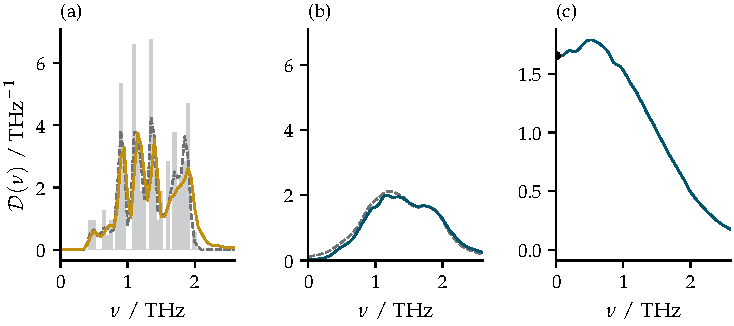
\includegraphics{ch16_observables/vdos}
\caption{(a) The vibrational density of states of the fcc crystal at
\SI{21}{\kelvin} at fixed energy, against the histogram of the harmonic
frequencies of the same cell (bars) and those frequencies passed through
the same window and transform (dashed). (b) The crystal under Langevin
friction of \SI{2}{\per\pico\second}, against the fixed-energy spectrum
spread by a Lorentzian of full width $\gamma/2\pi$ (dashed). (c) Liquid
argon at fixed energy, with $12mD/\kB T$ at $\nu = 0$ (point).}
\label{fig:ob-vdos}
\end{figure}

\begin{figure}[htb]
\centering
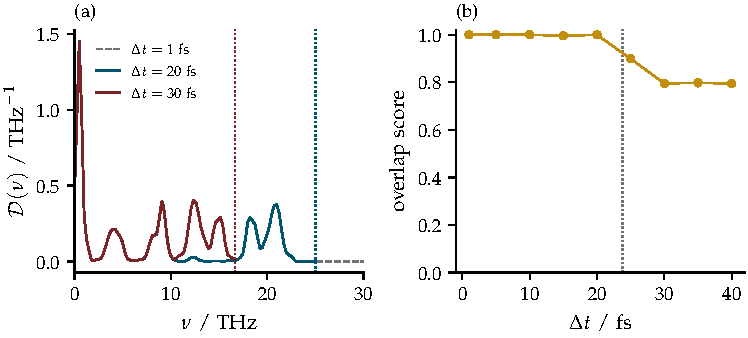
\includegraphics{ch16_observables/stride}
\caption{The four-bead chain at fixed energy, 20 copies, velocities
every \SI{1}{\femto\second} with each copy's centre-of-mass velocity
removed. (a) The vibrational density of states from every frame
(dashed), from every 20th and from every 30th, each to its own Nyquist
frequency (dotted lines). (b) The overlap score of the spectrum from
every $\Delta t$-th frame with that from every frame, both cut at the
Nyquist frequency of $\Delta t$, against $\Delta t$; the dotted line
marks $1/2\nu_{\mathrm b}$, with $\nu_{\mathrm b}$ the frequency of the
highest peak.}
\label{fig:ob-stride}
\end{figure}

\subsection*{How often an atom tries}

Chapter~12 noted that how often an atom hops depends also on how often it
tries, and left the measurement to this chapter. A lithium atom in a
hollow of the model surface vibrates, and each swing towards a bridge is
an attempt. Its density of states (\cref{fig:ob-layers}c) peaks at 5.25
and \SI{5.00}{\tera\hertz} at 600 and \SI{1000}{\kelvin}, below the
\SI{5.87}{\tera\hertz} of small vibrations in the hollow, because the
hollow widens as the atom climbs. That frequency is $\nu_0 =
\sqrt{k/m}/2\pi$, with $k$ the curvature of the energy at the bottom of
the hollow (\cref{sec:os-small}). Near a hollow each of the model's three
ripples (\cref{sec:en-surface}) has $\cos(\vb{g}_k\cdot\vb{r}) \approx 1 -
(\vb{g}_k\cdot\vb{r})^2/2$, and the squared cosines of the angles between
$\vb{r}$ and the three $\vb{g}_k$, \ang{120} apart, add to $\frac32$, so the
energy rises as $\frac{3}{16}U_{\mathrm b}\lvert\vb{g}\rvert^2r^2$ and $k =
3U_{\mathrm b}\lvert\vb{g}\rvert^2/8 = 2\pi^2U_{\mathrm b}/a^2 =
\SI{0.9785}{\electronvolt\per\angstrom\squared}$. With six bridges out of each hollow,
the estimate $6\nu\,\mathrm{e}^{-\beta U_{\mathrm b}}$ with this $\nu$
gives 0.095 and 0.923 hops per picosecond, against 0.134 and 0.898
counted and the transition-state rates 0.162 and 1.257 of
\cref{eq:th-tst}. The estimate takes the attempt frequency from the
spectrum and ignores how wide the passage over each bridge is compared
with the hollow, and it lies within a factor of 1.41 of the counted
rates: the frequency of attempts and the Boltzmann factor of the barrier
give a rate's size, and the counted hops give its value.

\begin{keyidea}
The vibrational density of states is the Fourier transform of the
mass-weighted velocity autocorrelation function, with area three per
atom; for a harmonic solid it is the histogram of the normal-mode
frequencies, and at zero frequency it is $12mD/\kB T$. Friction widens
each peak by $\gamma/2\pi$. Frames a stride $\Delta t$ apart show
frequencies only up to $1/2\Delta t$ and fold faster ones below it, so
spectra are compared at the same stride, by an overlap score.
\end{keyidea}

\notebook{16}{set the length of the correlation window and the stride, and watch the spectrum}

\begin{selfcheck}
The spectrum of one atom of a liquid is computed with $C_m$ cut at
\SI{1}{\pico\second}. Roughly how close can two peaks be and still be
seen as two?
\end{selfcheck}

%=============================================================================!
% 16.11  FREE ENERGY FROM A HISTOGRAM                                         !
%=============================================================================!
\section{Free energy from a histogram}
\label{sec:ob-fes}

A trajectory spends more time in some arrangements than in others. At
equilibrium these populations measure free-energy differences. A
histogram of a distance, angle or position therefore gives a free-energy
profile along that coordinate, provided the run has sampled it adequately.
We test this construction on a surface and a four-bead chain, where the
answer is known, then examine why rare crossings make the uncertainty
hard to estimate.

\subsection*{Free energy along a coordinate}

In the canonical ensemble the positions have the density $\mathcal{P}
\propto \mathrm{e}^{-\beta U}$ (\cref{sec:sm-canonical}). For a coordinate
$x$ computed from the positions, the density of its values is the total
weight of all arrangements with that value, and writing it as a Boltzmann
factor defines the free energy along $x$:
\begin{equation}
   \mathcal{P}(x) \propto \mathrm{e}^{-\beta F(x)} , \qquad
   F(x) = -\kB T\ln\mathcal{P}(x) + \text{constant} ,
   \label{eq:ob-fes}
\end{equation}
the free energy $-\kB T\ln Z$ of \cref{sec:sm-canonical} for the
arrangements held at that $x$. If $x$ is every coordinate of the system,
$F = U$ up to a constant. If it is fewer, $F$ includes the number of
arrangements that share each value, an entropy, and can differ from any
energy. A free-energy profile from a run is a histogram of $x$, as for
$g(r)$, turned into $F$ by \cref{eq:ob-fes}. Its error comes from blocks,
as in Chapter~15: the histogram of each block, normalised to a density;
the mean and the standard error of each bin over the blocks; and, since a
small change $\delta\mathcal{P}$ changes $\ln\mathcal{P}$ by
$\delta\mathcal{P}/\mathcal{P}$, an error of $\kB T\,\delta\mathcal{P}/
\mathcal{P}$ in $F$. \texttt{mdlab.analysis.landscape} does this for one
coordinate or several:

\begin{code}
def free_energy(
    values: ArrayLike,
    bins: int | ArrayLike | list,
    temperature: float,
    n_blocks: int = 10,
    value_range: list | None = None,
) -> tuple[list[NDArray], NDArray, NDArray]:
    x = np.asarray(values, dtype=float)
    x = x[:, None] if x.ndim == 1 else x
    edges = np.histogramdd(x, bins=bins, range=value_range)[1]
    blocks = np.array_split(x, n_blocks)
    density = np.array(
        [np.histogramdd(b, bins=edges, density=True)[0] for b in blocks]
    )
    p = density.mean(axis=0)
    dp = density.std(axis=0, ddof=1) / np.sqrt(n_blocks)
    kt = KB * temperature
    with np.errstate(divide="ignore", invalid="ignore"):
        f = -kt * np.log(p)
        df = kt * dp / p
    f -= np.min(f[np.isfinite(f)])
    middles = [0.5 * (e[1:] + e[:-1]) for e in edges]
    return middles, f, df
\end{code}

\subsection*{An atom on a surface}

A lithium atom on the model surface of \cref{sec:en-surface} has two
coordinates, and its position is all of them, so $F(x, y)$ must equal
$U(x, y)$. 1000 atoms at \SI{600}{\kelvin} under Langevin friction of
\SI{1}{\per\pico\second}, every \SI{50}{\femto\second} for
\SI{200}{\pico\second}, folded into one cell of the hollows, give the map
of \cref{fig:ob-fes}(a). A profile is tested against an exact one by the
mean of its squared misses divided by their squared errors. Each such
ratio has the mean 1 when the errors are right and, for misses of
Gaussian density, the variance $\ens{z^4} - 1 = 2$, so over $n$ independent bins the
mean scatters about 1 by $\sqrt{2/n}$; a mean of $c$ says that the
errors understate the misses by about $\sqrt c$. Below
\SI{0.3}{\electronvolt}, over 1400 bins, $F$ less $U$ gives 1.20, where
independent bins with correct errors would give $1.00 \pm 0.04$.
Histogram bins are correlated, so this spread is only a guide: it is constant to within about
1.1 times its errors, and the largest miss is
\SI{15.2}{\milli\electronvolt}.

The distance $r_{\mathrm h}$ from the nearest hollow is one coordinate of the two,
and $F(r_{\mathrm h})$ is not $U$. The positions at a distance $r_{\mathrm h}$ fill a circle of
circumference $2\pi r_{\mathrm h}$, so the density of $r_{\mathrm h}$ is
\begin{equation*}
   \mathcal{P}(r_{\mathrm h}) \propto r_{\mathrm h}\oint\mathrm{e}^{-\beta U(r_{\mathrm h}, \theta)}\,\dd\theta ,
   \qquad
   F(r_{\mathrm h}) = -\kB T\ln\Bigl[r_{\mathrm h}\oint\mathrm{e}^{-\beta U(r_{\mathrm h}, \theta)}\,\dd\theta
   \Bigr] ,
\end{equation*}
with $\theta$ the angle around the hollow, valid out to $a/2 =
\SI{1.23}{\angstrom}$, where the circle still lies in the region nearer
that hollow than any other. The factor $r_{\mathrm h}$ is the number of positions at
each distance, and it makes $F$ rise as $r_{\mathrm h} \to 0$, where $U$ is lowest:
there are few places that close to the centre, as there are few
velocities with all three components near zero in Maxwell's density of
speeds (\cref{sec:sm-maxwell}). The run's $F(r_{\mathrm h})$ follows
this within its errors, its squared misses over squared errors averaging
0.60 over 40 bins (\cref{fig:ob-fes}b), and its least value lies at $r_{\mathrm h} =
\SI{0.225}{\angstrom}$ from the hollow. For small $r_{\mathrm h}$, $U \approx
\frac12 kr_{\mathrm h}^2$ with $k = 3U_{\mathrm b}\lvert\vb{g}\rvert^2/8 =
2\pi^2U_{\mathrm b}/a^2$ (\cref{sec:ob-vdos}), so $\mathcal{P}
\propto r_{\mathrm h}\,\mathrm{e}^{-\beta kr_{\mathrm h}^2/2}$, whose largest value is at $r_{\mathrm h} =
\sqrt{\kB T/k} = \SI{0.230}{\angstrom}$. At the smallest $r_{\mathrm h}$, $F$ is
\SI{116}{\milli\electronvolt} above its least. A free-energy profile along
a coordinate carries the count of arrangements at each value, and a
minimum of $F$ need not be a minimum of $U$.

\subsection*{A dihedral angle}

The free energy of a dihedral angle is how the TrajCast paper judges the
slow motions of a molecule\cite{Thiemann2026}, and a model chain has an
exact answer for it. The chain has four beads of \SI{14.5}{\amu}, each
standing for a CH$_2$ or CH$_3$ group, joined by springs in the force
field of \cref{eq:pe-opls}: bonds with $\kappa_r =
\SI{5}{\electronvolt\per\angstrom\squared}$ and $r_{\mathrm{eq}} =
\SI{1.53}{\angstrom}$, angles with $\kappa_\theta =
\SI{2.5}{\electronvolt\per\radian\squared}$ and $\theta_{\mathrm{eq}} =
\ang{112}$, and a torsion with $\kappa_1 = 0.06$, $\kappa_2 = -0.01$ and
$\kappa_3 = \SI{0.12}{\electronvolt}$, which puts the lowest well at
$\psi = \ang{180}$ (trans), two gauche wells \SI{36.4}{\milli
\electronvolt} higher at $\pm\ang{63.7}$, barriers of
\SI{127.8}{\milli\electronvolt} at $\pm\ang{118.1}$ and
\SI{180}{\milli\electronvolt} at \ang{0}. The constants are chosen for
illustration. The forces of \texttt{mdlab.forcefield.BondedModel} match
finite differences of its energy to \SI{1e-8}{\electronvolt\per\angstrom}.

With no other terms, the density of $\psi$ is exactly $\mathrm{e}^{-\beta
U_{\mathrm t}(\psi)}$, $U_{\mathrm t}$ the torsion energy. Building the
chain bead by bead, the second bead's position relative to the first is
given by a length and two angles, the third's relative to the second by
$r_2$, the bond angle $\theta_1$ and an angle about the first bond, and
the fourth's by $r_3$, $\theta_2$ and its angle about the middle bond,
which is $\psi$. Each step is a set of spherical coordinates: small
changes of $r$, of $\theta$ and of the angle $\phi$ about the axis move the
bead by $\dd r$, $r\,\dd\theta$ and $r\sin\theta\,\dd\phi$ at right angles
to one another, a small volume $r^2\sin\theta\,\dd r\,\dd\theta\,\dd\phi$.
The volume for the whole chain is a product of such factors of $r$ and
$\sin\theta$ times $\dd\psi$, with no factor that depends on $\psi$. The energy is a sum of a part in the bonds and angles
and a part in $\psi$, so integrating over everything but $\psi$ leaves
$\mathrm{e}^{-\beta U_{\mathrm t}(\psi)}$ times a constant, and $F(\psi) =
U_{\mathrm t}(\psi)$ up to a constant.

Two hundred copies, each started in the trans well, are held by Langevin
friction of \SI{1}{\per\pico\second} at \SI{300}{\kelvin} and at
\SI{200}{\kelvin} for \SI{2}{\nano\second}, $\psi$ recorded every
\SI{100}{\femto\second}, and the first \SI{200}{\pico\second} left out:
over it the trans well holds 0.720 and 0.903 of the copies, against the
0.664 and 0.801 of equilibrium. Each bin of $F(\psi)$ is compared with
$-\kB T\ln$ of the bin's average of $\mathrm{e}^{-\beta U_{\mathrm t}}$,
since a histogram counts the whole bin. At \SI{300}{\kelvin}, where each
copy changes well 83.5 times per nanosecond, $F$ matches the torsion
energy within its errors (\cref{fig:ob-fes}c): the mean of the squared
misses over squared errors is 1.02 over 72 bins with blocks in time and
0.68 with blocks of 20 copies each, and at $\psi \approx 0$ the run gives
$(181 \pm 2)$\,\si{\milli\electronvolt} against 179.

At \SI{200}{\kelvin} each copy changes well only 8.0 times per
nanosecond, and the profile is harder to get right. Its shape is right,
$F(0) = (177 \pm 4)$\,\si{\milli\electronvolt} against 179, but with blocks
in time the squared misses over squared errors average 3.26, and they lie
mostly on one side, where counts are plentiful: 7.8 between $-\ang{120}$
and 0, 1.3 between 0 and \ang{120}. Over the \SI{1.8}{\nano\second} kept,
the gauche well near $+\ang{64}$ holds $0.0158 \pm 0.0088$ more of the
copies than the one near $-\ang{64}$, though by symmetry the two must hold
equal shares. That is
1.8 of its errors, an ordinary fluctuation when the error is taken over
the 200 independent copies; but each copy stays in a well for
\SI{125}{\pico\second} on average, so the populations of consecutive blocks in time
are not independent and their spread understates the error, by the mechanism of
\cref{sec:cv-blocks}. Blocks of copies instead give errors 40\% larger
(a median of 0.92 against \SI{0.66}{\milli\electronvolt}) and a mean of
2.05, much of what remains being that single fluctuation, which moves
every bin of a well together: folding $\psi$ to $\lvert\psi\rvert$, which
pools the two gauche wells and so cancels it, brings the mean to 1.06
with blocks of copies, while blocks in time still give 2.10. Free-energy profiles across barriers
crossed rarely need their error bars from independent runs, or from
blocks far longer than the time between crossings.

\begin{practice}
A free-energy profile is no better than the number of crossings between
its wells, and counting them is the check. For a two-well process with independent, approximately exponential stays,
$n$ crossings mean each side
is visited about $n/2$ times, its share of the time known to about
$\sqrt{2/n}$ of itself, so the ratio of the two shares is known to about
$2/\sqrt n$, and the difference of free energy to $2\kB T/\sqrt n$: two
thirds of $\kB T$ for ten crossings and a tenth for 400, whatever the
number of frames. Copies started in different wells, errors taken over
independent copies, and the start left out, where the wells still hold
the populations they began with, guard against the rest.
\end{practice}

\subsection*{The distribution of the potential energy}

The density of the potential energy itself is a profile of the same kind,
and the TrajCast paper compares it between a learned model and the
reference\cite{Thiemann2026}. It depends on the ensemble as well as the
forces: Chapter~15's liquid argon spreads by 0.677 under CSVR and by
\SI{0.532}{\milli\electronvolt} per atom at fixed energy, and the two
distributions overlap by 0.882 by the score of \cref{sec:ob-vdos}, against
0.980 for the two halves of the same CSVR run. A test of a model by this
distribution is a test of its forces only when both runs sample the same
ensemble; with that settled, a score near the halves' own is the target.

\begin{figure}[htb]
\centering
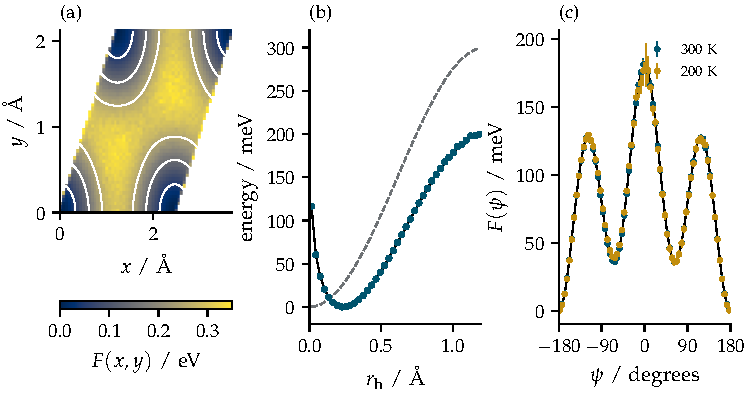
\includegraphics{ch16_observables/fes}
\caption{(a) Lithium on the model surface at \SI{600}{\kelvin}, positions
folded into one cell of the hollows: $F(x, y)$ (shading, \SIrange{0}{0.35}{
\electronvolt}, with its additive constant aligned to $U$) and contours of $U$ every \SI{0.1}{\electronvolt} (lines).
(b) The same atoms' free energy against the distance $r_{\mathrm h}$ to the nearest
hollow (points, with twice their errors), against the exact
$-\kB T\ln[r_{\mathrm h}\oint\mathrm{e}^{-\beta U}\dd\theta]$ (line) and $U$ along the
line from a hollow to a bridge (dashed). (c) The four-bead chain's
dihedral angle at 300 and \SI{200}{\kelvin}: $F(\psi)$ with twice its
error from ten blocks of 20 copies, after the first
\SI{200}{\pico\second}, against the torsion energy (line).}
\label{fig:ob-fes}
\end{figure}

\begin{keyidea}
The free energy along a coordinate is $-\kB T\ln$ of the density of its
values, estimated by a histogram, with errors from blocks. It equals the
potential energy only when the coordinate is every coordinate; otherwise
it counts the arrangements at each value. Across barriers crossed rarely,
short blocks in time underestimate errors; use sufficiently long blocks
or independent copies.
\end{keyidea}

\notebook{16}{build F from a histogram and watch the error bars at 200 K}

\begin{selfcheck}
Why does $F(r_{\mathrm h})$ for the lithium atom rise towards $r_{\mathrm h} = 0$ although the
potential energy is lowest there?
\end{selfcheck}

%=============================================================================!
% 16.12  WHAT THE TRAJECTORY LOOKS LIKE                                       !
%=============================================================================!
\section{What the trajectory looks like}
\label{sec:ob-trajectory}

The observables of this chapter are computed after the run, from saved
frames, and most of their faults are made then: in the frames chosen, in
how they are prepared, or in where a curve is read. A healthy set of
observables checks itself through the identities derived above. For the
liquid argon of this chapter, $g(r)$ with the pair potential gives the
run's energy and pressure, to 0.6 and 0.2 of their errors (\cref{sec:ob-rdf}); $S(G)$ from the positions agrees with
the transform of $g(r)$ where the cut at half the cell does not matter
and tends to $\rho\kB T\kappa_T$ at small $G$ (\cref{sec:ob-sq}); the slope
of the MSD and the integral of $C_{vv}$ give the same $D$
(\cref{sec:ob-vacf}); the density of states has the value $12mD/\kB T$
at zero frequency (\cref{sec:ob-vdos}); and where
the free energy is known exactly, the histogram reproduces it within its
errors (\cref{sec:ob-fes}). Each of these fails, in a recognisable way,
when something has gone wrong. \Cref{fig:ob-faults} and
\cref{tab:ob-faults} show six faults on liquid argon and gather those of
earlier sections.

\textit{Wrapped positions.} Positions put back into the cell, as most
trajectory files store them, give an MSD that jumps whenever an atom
crosses a face. From the run of \cref{sec:ob-msd} wrapped every
\SI{100}{\femto\second}, it is \SI{167.8}{\angstrom\squared} at
\SI{20}{\pico\second} against the true 45.2, and 222.0 and
\SI{258.0}{\angstrom\squared} at 50 and \SI{100}{\pico\second}, levelling
off towards \SI{270}{\angstrom\squared}, $L^2/2$, the mean squared distance
between two points placed at random in the cell (\cref{fig:ob-faults}a). The check is
the largest move between frames, which must be a small fraction of the
cell (\texttt{diagnostics.largest\_jump}, \cref{sec:cs-trajectory}), and
the cure is unwrapping (\texttt{diagnostics.unwrap}).

\textit{A drift of the centre of mass.} Starting velocities drawn without
removing their total momentum give the centre of mass a speed of about
$\sqrt{3\kB T/Nm}$, \SI{1.80e-4}{\angstrom\per\femto\second} here, which
it keeps for ever at fixed energy. Added to the same paths, it makes
the MSD curve upwards and the fit over 2 to \SI{20}{\pico\second} give $D$
31\% too high (\cref{fig:ob-faults}b); removing the centre of mass, as
\texttt{msd} does by default, restores \num{3.764e-4}. The check is the
path of the centre of mass (\texttt{diagnostics.centre\_of\_mass\_path}).

\textit{A fit in the ballistic part.} A window that ends before the motion
has forgotten its velocity fits a straight line to a curve: over 0.02 to
\SI{0.2}{\pico\second} it gives $D$ a third too low, while windows starting
at \SI{0.05}{\pico\second} or later and ending ten times later agree with
the 2 to \SI{20}{\pico\second} value within 6\% (\cref{fig:ob-faults}c). The
check is the slope of $\ln\text{MSD}$ against $\ln t$, which must be 1
over the window.

\textit{$g(r)$ past half the cell.} Separations reduced to their nearest
image cannot exceed half the cell's width along any axis, so beyond
$L/2$ the shells are partly empty. Computed out to \SI{16}{\angstrom} in
the 256-atom cell of side \SI{23.26}{\angstrom}, $g$ falls to 0.50 at
\SI{14}{\angstrom}, where the 2048-atom liquid shows 1.010
(\cref{fig:ob-faults}d). \texttt{rdf} refuses a range beyond half the
smallest width, as the cell list does.

\textit{Transport under a local thermostat.} Langevin friction of
\SI{10}{\per\pico\second} damps every velocity: $C_{vv}$ falls to half its
first value in \SI{60}{\femto\second} instead of 160, and to zero in 170
instead of 320, and its integral gives $D = \SI{0.682e-4}{\angstrom\squared\per
\femto\second}$, 82\% below the value at fixed energy
(\cref{fig:ob-faults}e). Transport coefficients and spectra come from runs
at fixed energy or under a global thermostat such as CSVR, which
Chapter~15 found leaves $D$ unchanged within its error; under friction
they belong to the friction (\cref{sec:th-langevin}).

\textit{A Green-Kubo integral read too late.} The integral of a
correlation function settles when the correlation has died and then
wanders as noise accumulates. For one \SI{1}{\nano\second} run of 256
atoms the shear viscosity read at \SI{2}{\pico\second}, on the plateau, is
\SI{2.18e-4}{\pascal\second}, 18\% above the \num{1.853e-4} from all
\SI{14}{\nano\second}, the spread of a single run; read later, at 10, 20
and \SI{40}{\pico\second}, it is 1.91, 1.78 and \num{2.01e-4}
(\cref{fig:ob-faults}f), wandering by as much again. The check is to read
the plateau where the correlation has died, here 1 to
\SI{3}{\pico\second}, and to take the error from independent runs.

\begin{figure}[htb]
\centering
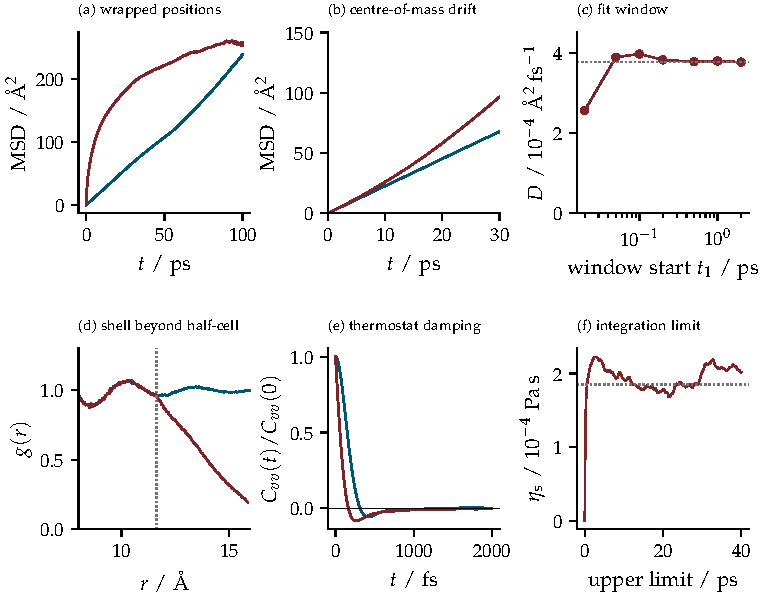
\includegraphics{ch16_observables/faults}
\caption{Six faults on liquid argon, each against the correct curve
(teal). (a) The MSD from positions wrapped into the cell. (b) The MSD of
paths whose centre of mass drifts at $\sqrt{3\kB T/Nm}$, not removed. (c)
$D$ fitted to windows from $t_1$ to $10t_1$, against $t_1$, with the 2 to
\SI{20}{\pico\second} value (dotted). (d) $g(r)$ of the 256-atom cell taken
past half its side (dotted) with the nearest image, against the
2048-atom $g(r)$. (e) $C_{vv}$ under Langevin friction of
\SI{10}{\per\pico\second}. (f) The Green-Kubo integral of the shear stress
from one \SI{1}{\nano\second} run, read out to \SI{40}{\pico\second},
against the value from \SI{14}{\nano\second} (dotted).}
\label{fig:ob-faults}
\end{figure}

\begin{table}[htb]
\centering
\small
\caption{Faults of observables, the check that finds each, and its size
in this chapter's runs.}
\label{tab:ob-faults}
\begin{tabular}{@{}>{\raggedright\arraybackslash}p{0.29\linewidth}
   >{\raggedright\arraybackslash}p{0.36\linewidth}
   >{\raggedright\arraybackslash}p{0.29\linewidth}@{}}
\toprule
fault & check & measured\\
\midrule
wrapped positions in an MSD & largest move between frames; unwrap &
\SI{168}{\angstrom\squared} at \SI{20}{\pico\second}, not 45\\
centre of mass drifting & path of the centre of mass; remove it & $D$
31\% high\\
fit in the ballistic part & slope of $\ln$MSD against $\ln t$ is 1 & $D$
32\% low\\
$g(r)$ past half the cell & range at most half the smallest width & $g =
0.50$ at \SI{14}{\angstrom}, not 1.01\\
transport under friction & run at fixed energy or with CSVR & $D$ 82\%
low at \SI{10}{\per\pico\second}\\
Green-Kubo read too late & read the plateau; errors from runs &
$\eta_{\mathrm s}$ from 1.78 to \num{2.18e-4}\\
bonds from one cutoff & band of hysteresis; least lifetime & 3.2 times
the events (\cref{sec:ob-bonds})\\
frames too sparse for a spectrum & stride below $1/2\nu_{\max}$; same
stride for both & overlap 0.795 at \SI{30}{\femto\second}
(\cref{sec:ob-vdos})\\
errors of $F$ from short blocks & errors over independent copies &
squared misses over squared errors 3.26, not 1 (\cref{sec:ob-fes})\\
energy distributions from two ensembles & same thermostat for both &
overlap 0.882, not 0.980 (\cref{sec:ob-fes})\\
\bottomrule
\end{tabular}
\end{table}

\begin{keyidea}
Observables check one another: $g(r)$ gives the energy and the pressure,
the MSD and the velocity autocorrelation give the same $D$, and the
density of states holds $D$ at zero frequency. Their common faults
are wrapped positions, an unremoved drift, a fit window in the ballistic
part, a range past half the cell, transport under a local thermostat, an
integral read too late, frames too sparse, and error bars from blocks
shorter than the slowest motion.
\end{keyidea}

\notebook{16}{break each observable and find the check that catches it}

\begin{selfcheck}
An MSD from a long run levels off at a value close to $L^2/2$. What is
the most likely fault?
\end{selfcheck}

%=============================================================================!
% 16.S  WHAT WE NOW HAVE                                                      !
%=============================================================================!
\unnumbered{What we now have}

The radial distribution function counts the partners at each distance
against an even scatter, a histogram of pair distances out to half the
cell that tends far away to $1 - S(0)/N$ in a fixed cell, $1 - 1/N$ for
atoms placed at random; with the pair potential and the kinetic energy it
gives the energy and the pressure, and with its short memory it converges
several times sooner than the pressure. Its transform is the structure factor
that diffraction measures, computed from the positions on the cell's own
wave vectors where the cut at half the cell would spoil it, and tending
to $\rho\kB T\kappa_T$ at long wavelengths.
Bonds are assigned from
distances with a band of hysteresis and a least lifetime, stored as
whole-number keys whose sorted lists give the bonds formed and broken;
molecules are the connected components of their graph, species their
formula and a hash of their bonding; reactions are changes of the
molecules that atoms belong to, and rates are counts over exposures with
the error $\sqrt n$; the ratio of the rate constants of a reaction and
its reverse is an equilibrium constant that statistical mechanics
predicts. Observers do this as the run goes, at about a tenth of the cost
of a cheap force evaluation.
The mean squared displacement grows as $2dDt$, from unwrapped
paths with the centre of mass removed, and equals twice the integral of
the velocity autocorrelation function weighted by $t - s$, so $D$ is also
a Green-Kubo integral; the shear viscosity is another, and its value,
$(1.853 \pm 0.038)\times10^{-4}$\,\si{\pascal\second} for liquid argon,
lies 1.6 combined errors from the one that Chapter~15 inferred from the
change of $D$ with the size of the box.
Independent ions conduct as $\sum_iq_i^2D_i/V\kB T$,
and the Haven ratio measures how far correlated ions fall short of it;
in layers, $D$ becomes a tensor; and hops between sites give $D =
fk_{\mathrm h}a^2/4$, with a correlation factor $f$ that friction brings to 1.
The Fourier transform, computed in $N_{\mathrm s}\log_2N_{\mathrm s}$
operations for $N_{\mathrm s}$ samples, turns the velocity
autocorrelation function into the vibrational density of states, whose
peaks are the normal modes, whose width grows by $\gamma/2\pi$ under
friction, whose value at zero holds $D$, and which frames a stride
$\Delta t$ apart show only up to $1/2\Delta t$.
A histogram of any
coordinate gives its free energy, which counts arrangements as well as
energies, with error bars that must come from independent runs when the
barriers are crossed rarely.

Chapter~17 runs these analyses on the simulations they are meant for:
ASE and LAMMPS with a learned potential, lithium in graphite, and the
trajectory gallery of every fault met so far.

%=============================================================================!
% 16.A  ANSWERS TO THE CHECKS                                                 !
%=============================================================================!
\unnumbered{Answers to the checks}
\label{sec:ob-answers}

\answerto{sec:ob-rdf}$1 - 1/500 = 0.998$. Each atom's partners are the
other $N - 1$, while the divisor assumes $N$; a larger cell at the same
density holds more atoms, so $1/N$ is smaller and the far value closer
to 1.

\answerto{sec:ob-sq}At a vector of the crystal's reciprocal lattice every
phase $\vb{G}\cdot\vb{r}_{ij}$ is a multiple of $2\pi$, every arrow points
the same way, and $S(\vb{G}) = N$. At an allowed vector of the cell that is not
one of these, the arrows of the identical unit cells are turned through
equal steps that come round to the start after a whole number of turns,
so they sum to zero and $S(\vb{G}) = 0$.

\answerto{sec:ob-bonds}None: $342\,017$ would be $i = 342$, $j = 17$, but
every key has $i < j$. The bond between atoms 17 and 342 has the key
$17\,342$ only.

\answerto{sec:ob-reactions}$1/\sqrt{25} = 0.20$, to a fifth. Halving it
needs four times as many events, 100.

\answerto{sec:ob-msd}Near $t = 2Dm/\kB T$. With $m = \SI{40}{\amu}$, $D =
\SI{3e-4}{\angstrom\squared\per\femto\second}$ and $T = \SI{300}{\kelvin}$
this is \SI{96}{\femto\second}.

\answerto{sec:ob-vacf}$D$ is a third of the whole integral of $C_{vv}$.
After the dip begins, $C_{vv}$ is negative and its integral subtracts from
what the positive part gave: on average the atom moves back after it
rebounds from its neighbours, which undoes part of its displacement.

\answerto{sec:ob-charge}Each pair moves $\vb{M}_q$ by $e(\Delta\vb{r}_+ -
\Delta\vb{r}_-)$, which stays bounded while the two stay together, so the
mean squared displacement of $\vb{M}_q$ stops growing and $\sigma_{\mathrm e}
= 0$. $\sigma_{\mathrm{NE}}$ still counts every ion's own diffusion and is
not zero, so $H_{\mathrm R}$ would be without bound.

\answerto{sec:ob-layers}Each hop moves the atom by $a$ in one of six
directions, so after $n = k_{\mathrm h}t$ hops the MSD is $k_{\mathrm h}ta^2 = 6Dt$,
and $D = k_{\mathrm h}a^2/6$.

\answerto{sec:ob-fourier}The Nyquist frequency is $1/(2\times
\SI{20}{\femto\second}) = \SI{25}{\tera\hertz}$, and \SI{30}{\tera\hertz}
folds to $50 - 30 = \SI{20}{\tera\hertz}$.

\answerto{sec:ob-vdos}About $1/t_{\mathrm c} = \SI{1}{\tera\hertz}$: peaks
closer than that blur into one.

\answerto{sec:ob-fes}The positions a distance $r_{\mathrm h}$ from the hollow fill a
circle of circumference $2\pi r_{\mathrm h}$, so the density of $r_{\mathrm h}$ carries the factor
$r_{\mathrm h}$, which vanishes at the centre. There are few places that close,
however low their energy, and $F = -\kB T\ln\mathcal{P}$ rises without
bound as $r_{\mathrm h} \to 0$.

\answerto{sec:ob-trajectory}Positions wrapped into the cell: $L^2/2$ is
the mean squared distance between two points placed at random in a cube
of side $L$, which is what the MSD of wrapped positions approaches.

%=============================================================================!
% 16.E  EXERCISES                                                             !
%=============================================================================!
\unnumbered{Exercises}
\label{sec:ob-exercises}

The exercises run from questions of understanding, through calculations,
to short derivations marked `show that'. Full solutions are in
\hyperref[sec:ob-solutions]{`Solutions to the exercises'} at the end of
the book, and Notebook~16 checks every numerical answer.

\begin{exercise}[the volume of a shell]
\label{ex:ob-shell}
For bins of \SI{0.05}{\angstrom}, by what fraction does $4\pi r^2\,\delta r$
fall short of the exact volume of the shell from $r$ to $r + \delta r$,
at $r = 1$ and at \SI{5}{\angstrom}? Show that the fraction is close to
$\delta r/r$ when $\delta r \ll r$.
\end{exercise}

\begin{exercise}[the far value of g(r)]
\label{ex:ob-far}
What value does $g(r)$ approach far from any atom, with ASE's
normalisation, for 256 and for 2048 atoms placed independently at random?
Which normalisation would make it approach 1 for them, and why is the
difference unimportant for the coordination number of the first shell?
\end{exercise}

\begin{exercise}[the shells of a face-centred cubic crystal]
\label{ex:ob-fcc}
In the fcc lattice of cube side $a$, the atoms sit at the corners of the
cube and at the centres of its faces. Show that an atom's nearest
neighbours are $a/\sqrt2$ away and number 12, and that the next shell is
at $a$ and holds 6.
\end{exercise}

\begin{exercise}[structure without structure]
\label{ex:ob-meanfield}
Suppose $g(r) = 0$ for $r < \sigma$ and $g(r) = 1$ beyond. Show that the
Lennard-Jones energy per atom is then $-\frac{16}{9}\pi\rho\sigma^3
\varepsilon$, and evaluate it for liquid argon, $\rho\sigma^3 = 0.8$ and
$\varepsilon = \SI{0.01034}{\electronvolt}$. Compare it with
\SI{-56.16}{\milli\electronvolt}, the energy per atom that the run's $g(r)$
gives with the full Lennard-Jones potential (the run itself switches the
potential off between $2\sigma$ and $2.5\sigma$), and say what the
difference measures.
\end{exercise}

\begin{exercise}[random atoms and a perfect crystal]
\label{ex:ob-sq-limits}
Show from \cref{eq:ob-sq} that $S(\vb{G})$ averages to 1 for atoms placed
independently at random in the cell, at any allowed $\vb{G} \neq
\vb{0}$, and is $N$ for a perfect crystal at a vector of its reciprocal
lattice.
\end{exercise}

\begin{exercise}[compressibility from scattering]
\label{ex:ob-s0}
A liquid of number density \SI{0.03}{\per\angstrom\cubed} at
\SI{300}{\kelvin} has $\kappa_T = \SI{0.5}{\per\giga\pascal}$. What is
$S(0)$? Would a liquid twice as compressible scatter long waves more
strongly or less?
\end{exercise}

\begin{exercise}[flicker]
\label{ex:ob-flicker}
A bonded pair vibrates with a period of \SI{60}{\femto\second}, and the
far end of each vibration carries it beyond a single cutoff. How many
events per picosecond does the cutoff record for this one pair? With
$r_{\mathrm{on}}$ at the old cutoff, how wide must the band of hysteresis
be to record none, and how wide to record none wherever the cutoff falls
within the vibration?
\end{exercise}

\begin{exercise}[bonds as keys]
\label{ex:ob-keys}
Six atoms have the bonds 0-1, 1-2, 3-4 in one frame and 0-1, 2-3, 3-4,
4-5 in the next. Write both sets as keys $iN + j$ with $N = 6$, find the
bonds formed and broken by the merge of sorted lists, and find the
molecules of each frame by the search of the toolbox in \cref{sec:ob-bonds}.
\end{exercise}

\begin{exercise}[two graphs that look alike]
\label{ex:ob-hash}
Six atoms of one element form a triangular prism (two triangles, each
atom of one joined to the atom above it in the other); six others form
a hexagon with each atom also joined to the opposite one. Show that every
atom in both has three neighbours, and explain why every round of the
hash of \cref{sec:ob-bonds} then gives every atom of both the same
number. Are the two molecules the same?
\end{exercise}

\begin{exercise}[how many events]
\label{ex:ob-poisson}
A rate is wanted to 2\%. How many events must be counted? A run of
\SI{1}{\nano\second} of 100 molecules shows 40 dissociations: give the
rate per molecule with its error.
\end{exercise}

\begin{exercise}[a random walk in one dimension]
\label{ex:ob-walk}
An atom on a line hops by $+a$ or $-a$ with equal probability, at the
rate $k_{\mathrm h}$. Show that its MSD after a time $t$ is $k_{\mathrm
h}a^2t$ and that $D = k_{\mathrm h}a^2/2$.
\end{exercise}

\begin{exercise}[hops that keep their direction]
\label{ex:ob-correlated}
On a line, each step of length $a$ repeats the direction of the one
before with probability $\frac12(1 + c)$, so that consecutive steps have
the correlation $c$, and steps $k$ apart $c^k$. Show that for many steps
the MSD is $na^2(1 + c)/(1 - c)$, and so that $f = (1 + c)/(1 - c)$, the
statistical inefficiency of \cref{sec:cv-correlation}. What $c$ gives the
memory of direction, $4D/k_{\mathrm h}\ens{\ell^2} = 3.46$, of the model
surface at \SI{1}{\per\pico\second}?
\end{exercise}

\begin{exercise}[the end of the ballistic part]
\label{ex:ob-water}
For Chapter~11's water, $D = \SI{5.24e-4}{\angstrom\squared\per\femto
\second}$ at \SI{304}{\kelvin}. Estimate when a molecule's motion stops
being ballistic, taking its mass as \SI{18.015}{\amu}.
\end{exercise}

\begin{exercise}[an exponential memory]
\label{ex:ob-exp}
Show from \cref{eq:ob-msd-vacf} that $C_{vv} = C_0\mathrm{e}^{-t/\tau_{\mathrm
c}}$ gives $\text{MSD} = 2C_0\tau_{\mathrm c}[t - \tau_{\mathrm c}(1 -
\mathrm{e}^{-t/\tau_{\mathrm c}})]$, that this is $C_0t^2$ for $t \ll
\tau_{\mathrm c}$ and $2C_0\tau_{\mathrm c}t$ for $t \gg \tau_{\mathrm c}$,
and so that $D = C_0\tau_{\mathrm c}/3$.
\end{exercise}

\begin{exercise}[the viscosity on the back of an envelope]
\label{ex:ob-eta}
\Cref{tab:cv-observables} gives the shear stress of liquid argon a
spread of \SI{0.0121}{\giga\pascal} and an integrated correlation time of
\SI{0.18}{\pico\second}. Show that the Green-Kubo integral is $(V/\kB T)
\sigma_{xy}^2\tau_{\mathrm{int}}$, with $\sigma_{xy}$ the spread, and
evaluate it
for 256 atoms at \SI{0.02035}{\per\angstrom\cubed} and \SI{135}{\kelvin}.
\end{exercise}

\begin{exercise}[Nernst-Einstein for the salt]
\label{ex:ob-ne}
From the mean diffusion coefficients of \cref{sec:ob-charge}, $5.19$ and
$\SI{5.03e-4}{\angstrom\squared\per\femto\second}$ for 32 ions of each
kind in a cell of side \SI{13.4}{\angstrom} at \SI{1487}{\kelvin},
compute $\sigma_{\mathrm{NE}}$ in \si{\siemens\per\metre}.
\end{exercise}

\begin{exercise}[one number for layers]
\label{ex:ob-trace}
What would a single diffusion coefficient, a sixth of the slope of the
full MSD, report for the guests of \cref{sec:ob-layers}? Why does it
describe neither of their motions?
\end{exercise}

\begin{exercise}[Euler's formula at work]
\label{ex:ob-euler}
Show that $\lvert\mathrm{e}^{\mathrm{i}\theta}\rvert = 1$, and recover
$\cos(A + B)$ and $\sin(A + B)$ from $\mathrm{e}^{\mathrm{i}A}
\mathrm{e}^{\mathrm{i}B} = \mathrm{e}^{\mathrm{i}(A + B)}$.
\end{exercise}

\begin{exercise}[the transform of one cosine]
\label{ex:ob-dft-cos}
Show that the discrete transform of $x_n = \cos(2\pi mn/N_{\mathrm s})$,
for a whole number $0 < m < N_{\mathrm s}/2$, is $N_{\mathrm s}/2$ at $k =
m$ and at $k = N_{\mathrm s} - m$ and zero elsewhere.
\end{exercise}

\begin{exercise}[how fast is fast]
\label{ex:ob-fft-cost}
Show that $W(N_{\mathrm s}) = 2W(N_{\mathrm s}/2) + N_{\mathrm s}$ with $W(1)
= 0$ gives $W(N_{\mathrm s}) = N_{\mathrm s}\log_2N_{\mathrm s}$ for
$N_{\mathrm s}$ a power of 2, and find the ratio of $N_{\mathrm s}^2$ to
$N_{\mathrm s}\log_2N_{\mathrm s}$ for $N_{\mathrm s} = 2^{20}$.
\end{exercise}

\begin{exercise}[a stride that hides a bond]
\label{ex:ob-fold}
The chain's stretch at \SI{18.25}{\tera\hertz} is seen in frames every
\SI{35}{\femto\second}. Where does it appear? What is the longest stride
at which it appears where it is?
\end{exercise}

\begin{exercise}[friction against resolution]
\label{ex:ob-width}
A spectrum is computed from a run under Langevin friction of
\SI{1}{\per\pico\second} with correlations taken to \SI{10}{\pico\second}.
Which widens its peaks more, the friction or the window?
\end{exercise}

\begin{exercise}[diffusion in a spectrum]
\label{ex:ob-vdos-zero}
What is $\mathcal{D}(0)$, in \si{\per\tera\hertz}, for the oxygen atoms of
Chapter~11's water, $m = \SI{15.999}{\amu}$, with the $D$ of
\cref{ex:ob-water}?
\end{exercise}

\begin{exercise}[where the free energy is lowest]
\label{ex:ob-fd}
Show that for $U \approx \frac12kr_{\mathrm h}^2$ the free energy along the distance
$r_{\mathrm h}$ from a hollow, $F(r_{\mathrm h}) = -\kB T\ln[r_{\mathrm h}\,\mathrm{e}^{-\beta kr_{\mathrm h}^2/2}] +
\text{constant}$, is least at $r_{\mathrm h} = \sqrt{\kB T/k}$, and evaluate it at
\SI{300}{\kelvin} for $k = \SI{0.9785}{\electronvolt\per\angstrom\squared}$.
\end{exercise}

\begin{exercise}[crossings]
\label{ex:ob-crossings}
A run crosses a barrier between two wells $n$ times. Argue that the free
energy difference between the wells is known to about $2\kB T/\sqrt n$,
and find how many crossings give it to $0.1\,\kB T$.
\end{exercise}


%=============================================================================!
% CHAPTER 17  MD IN PRACTICE                                                  !
%=============================================================================!
\chapter{Molecular dynamics in practice}
\label{ch:practice}

%=============================================================================!
% 17.0 CHAPTER OPENING !
%=============================================================================!
The methods of Chapters~9 to~16 are now implemented in \texttt{mdlab}.
Research codes use the same physical ideas, but their units, defaults
and data formats differ. Moving a calculation between codes therefore
starts with a comparison whose answer we already know. Here we run the
same argon model in \texttt{mdlab}, the Atomic Simulation Environment
(ASE)\cite{Larsen2017} and LAMMPS\cite{Thompson2022}, tracing the
conversions needed for their results to agree.

We then use MACE-MP-0\cite{Batatia2025}, a \emph{foundation model}
trained on first-principles calculations across much of the periodic
table. Its broad training makes it useful on many materials, but does
not establish its accuracy on a particular system. We examine its cost
and time step, and use FHI-aims\cite{Blum2009} to measure the cost and
convergence of a first-principles reference. Here \emph{first-principles}
means that the forces are calculated from the electrons
(\cref{sec:pe-origin}) rather than supplied by a fitted interatomic model.

Lithium in graphite brings these choices together in a material that the
earlier chapters represented with model surfaces and layered solids.
Its spacing and hops require different convergence checks. A production
protocol collects those checks with the measurements that justify each
setting; the final gallery links the faults of a trajectory to the
checks that reveal them.

%=============================================================================!
% 17.1  MOLECULAR DYNAMICS WITH ASE                                           !
%=============================================================================!
\section{Molecular dynamics with ASE}
\label{sec:ip-ase}

A travel adaptor lets one plug fit the sockets of many countries: the
kettle is the same, and only the connection changes. The Atomic
Simulation Environment (ASE)\cite{Larsen2017} is such an adaptor for
atomistic calculations. One Python object holds the atoms, and any of
dozens of programs that compute energies and forces, from a pair
potential to a learned model or a first-principles code, can be plugged
into it as a \emph{calculator}; the same integrators, thermostats,
optimisers and file readers then work with every one of them. Earlier
chapters checked \texttt{mdlab}'s integrators and thermostats against
ASE's (\cref{sec:md-loop,sec:th-tests}); this section sets out how a run
is written in ASE, and runs \texttt{mdlab}'s own liquid argon through it.

\subsection*{Atoms, calculators and units}

An \texttt{ase.Atoms} object holds the chemical symbols, the positions in
\si{\angstrom}, the cell, the masses in \si{\amu} and the momenta. ASE
stores the lattice vectors as the \emph{rows} of the cell, where
\texttt{mdlab} stores them as the columns of $\vb{h}$ (\cref{sec:md-periodic}),
so one is the transpose of the other. A calculator attached to the atoms
answers \texttt{get\_potential\_energy}, \texttt{get\_forces} and
\texttt{get\_stress}, the last in \si{\electronvolt\per\angstrom\cubed}.
The stress is the pressure tensor of \cref{sec:pr-tensor} with its sign
reversed, so that a compressed solid has a negative stress. By default it
holds only the part from the forces; the kinetic part of
\cref{eq:pr-tensor} is added only with
\texttt{get\_stress(include\_\allowbreak ideal\_gas=True)}, whose omission
was a fault of \cref{sec:pr-trajectory}, and with it the pressure is minus
a third of the stress's trace.

ASE measures energy in \si{\electronvolt}, length in \si{\angstrom} and
mass in \si{\amu}, and computes an acceleration as force over mass with
no conversion factor. Its unit of time $t_{\mathrm A}$ is therefore the
one for which a force of \SI{1}{\electronvolt\per\angstrom} on
\SI{1}{\amu} gives \SI{1}{\angstrom} per $t_{\mathrm A}^2$, with the
joule, and so the electronvolt, being a mass times a length squared over
a time squared:
\begin{align*}
   \frac{\si{\electronvolt}}{\si{\angstrom}}
      &= \si{\amu}\,\frac{\si{\angstrom}}{t_{\mathrm A}^2}
      && \text{$F = ma$ with every number 1}\\
   t_{\mathrm A}^2 &= \frac{\si{\amu}\,\si{\angstrom}^2}{\si{\electronvolt}}
      && \text{multiplying by $t_{\mathrm A}^2\,\si{\angstrom}/
         \si{\electronvolt}$}\\
   t_{\mathrm A} &= \si{\angstrom}\sqrt{\frac{\si{\amu}}{\si{\electronvolt}}}
      && \text{taking the root}\\
   &= \SI{1e-10}{\metre}\times\sqrt{\frac{\SI{1.6605e-27}{\kilogram}}
        {\SI{1.6022e-19}{\kilogram\metre\squared\per\second\squared}}}
      && \text{in SI units}\\
   &= \SI{1e-10}{\metre}\times\SI{1.018e-4}{\second\per\metre}
      = \SI{10.18}{\femto\second} .
\end{align*}
A time step and a thermostat's time constant are given to ASE in this
unit, and a friction in its reciprocal. ASE supplies the femtosecond as
\texttt{ase.units.fs}, so a step of \SI{10}{\femto\second} is written
\texttt{10 * units.fs}, and a friction of \SI{0.001}{\per\femto\second}
\texttt{0.001 / units.fs}. Velocities are lengths per $t_{\mathrm A}$: an
atom that covers \SI{1}{\angstrom} in a femtosecond covers
\SI{10.18}{\angstrom} in one $t_{\mathrm A}$, so \texttt{mdlab}'s
velocities, in \si{\angstrom\per\femto\second}, are multiplied by 10.18 on
the way in, the factor whose omission was one of the faults of
\cref{sec:cs-trajectory}.

Any \texttt{mdlab} model becomes a calculator through
\texttt{mdlab.io.mdlab\_calculator}, which passes ASE's positions to the
model and its energy, forces and, from its virial, stress back:

\begin{code}
def mdlab_calculator(model):
    from ase.calculators.calculator import Calculator, all_changes
    class MdlabCalculator(Calculator):
        implemented_properties = ["energy", "free_energy", "forces",
                                  "stress"]

        def calculate(self, atoms=None, properties=("energy",),
                      system_changes=all_changes):
            super().calculate(atoms, properties, system_changes)
            h = np.array(self.atoms.get_cell()).T
            # any change at all, since a strain of 1e-5 must be seen
            if hasattr(model, "set_cell") and not np.array_equal(
                    h, model.cell):
                model.set_cell(h)
            energy, forces = model(self.atoms.get_positions())
            self.results = {"energy": float(energy),
                            "free_energy": float(energy),
                            "forces": np.array(forces)}
            if hasattr(model, "virial"):
                w = -np.asarray(model.virial) / self.atoms.get_volume()
                # Voigt order: xx, yy, zz, yz, xz, xy
                self.results["stress"] = w[[0, 1, 2, 1, 0, 0],
                                           [0, 1, 2, 2, 2, 1]]

    return MdlabCalculator()
\end{code}

\noindent The stress is $-\mathcal{W}_{\alpha\beta}/V$, the virial tensor of
\cref{sec:pr-tensor} over the volume, in ASE's order $xx$, $yy$, $zz$,
$yz$, $xz$, $xy$. A test strains the cell by $\pm\num{1e-5}$ in each of
its six components, three stretches and three shears, and compares the change of the energy with this stress, to
\SI{1e-8}{\electronvolt\per\angstrom\cubed}; the comment marks why the cell
is compared exactly, since a tolerance would hide so small a strain.

\subsection*{Dynamics}

An integrator in ASE is an object built on the atoms with a time step,
whose \texttt{run(n)} takes $n$ steps and calls any function attached
with \texttt{attach(f, interval)} every so many steps, as \texttt{mdlab}'s
observers do (\cref{sec:ob-reactions}). \texttt{VelocityVerlet} is the
integrator of \cref{sec:in-verlet}; \texttt{Langevin} adds the friction
and random kicks of \cref{sec:th-langevin}, with the friction $\gamma$ in
reciprocal time units; \texttt{Bussi} is CSVR (\cref{sec:th-csvr}); and
\texttt{NoseHooverChainNVT} is the chain of \cref{sec:th-nose}, but
counts $3N$ freedoms where \texttt{mdlab} counts $N_{\mathrm f}$: in its
first mass, $3N\kB T\tau_{\mathrm T}^2$ against $N_{\mathrm f}\kB
T\tau_{\mathrm T}^2$, and in its target, which raises the temperature of a
run whose centre of mass is still by $3N/N_{\mathrm f}$
(\cref{sec:th-trajectory}). For constant pressure, \texttt{IsotropicMTKNPT} is
the isotropic piston of \cref{sec:pr-piston}, \texttt{MTKNPT} lets every
component of the cell move, and \texttt{MaskedMTKNPT} lets chosen lattice
vectors change length while keeping their directions, which a layered
solid needs (\cref{sec:pr-shape}). \Cref{tab:ip-methods} sets these
beside \texttt{mdlab}'s and LAMMPS's.

One change in ASE's own advice shows why a version should be recorded
with every run. Its \texttt{Langevin} once held the centre of mass still
with an option, \texttt{fixcm}; from version 3.28 ASE warns that this
option does not sample the canonical ensemble exactly and asks for a
constraint, \texttt{FixCom}, instead. The runs below follow the warning.

\subsection*{The same liquid in two codes}

Chapter~12's liquid argon, 256 atoms of the switched Lennard-Jones model
at \SI{135}{\kelvin}, was run from one starting state by \texttt{mdlab}
and by ASE with \texttt{mdlab\_calculator}, with steps of
\SI{10}{\femto\second}, converted with \texttt{mdlab}'s constants rather
than \texttt{units.fs}, whose older constants put a difference of 4.6
parts in $10^9$ into the clock (\cref{sec:md-loop}). At fixed energy the
two runs share their energy to the last digit printed, its spread over
\SI{5}{\pico\second} being \SI{0.469}{\milli\electronvolt} in both, and
their positions differ by \SI{3.9e-14}{\angstrom} after
\SI{1}{\pico\second}, \num{3.1e-13} after 2 and \num{1.2e-10} after
\SI{5}{\pico\second} (\cref{fig:ip-codes}a). The two codes add the same
forces in different orders, and the chaos of \cref{sec:md-loop} amplifies
the rounding about 3000 times over the four picoseconds from 1 to
\SI{5}{\pico\second}, some seven times a picosecond, as it would any
difference.

Under the three thermostats, at a friction of \SI{1}{\per\pico\second} and
time constants of \SI{1}{\pico\second}, each code was run for
\SI{200}{\pico\second}. The mean temperatures lie within three standard
errors of \SI{135}{\kelvin}, the spreads of the kinetic temperature
within 0.989 and 1.016 of the canonical $\sqrt{2/N_{\mathrm f}}\,T$
(\cref{sec:sm-kinetic}), and the diffusion coefficients, from the MSD
over 2 to \SI{20}{\pico\second} in five blocks (\cref{sec:ob-msd}), agree
within their errors (\cref{fig:ip-codes}b): $(3.94 \pm 0.14)$ and
$(4.11 \pm 0.19)\times10^{-4}$\,\si{\angstrom\squared\per\femto\second}
under CSVR, $(3.92 \pm 0.05)$ and $(3.95 \pm 0.10)\times10^{-4}$ under the
chain, $(2.61 \pm 0.06)$ and $(2.66 \pm 0.08)\times10^{-4}$ under the
friction, which slows diffusion as \cref{sec:ob-trajectory} found. A step
costs \SI{1.32}{\milli\second} in \texttt{mdlab} and \SI{1.44}{\milli
\second} in ASE, since the forces are \texttt{mdlab}'s in both.

\begin{figure}[htb]
\centering
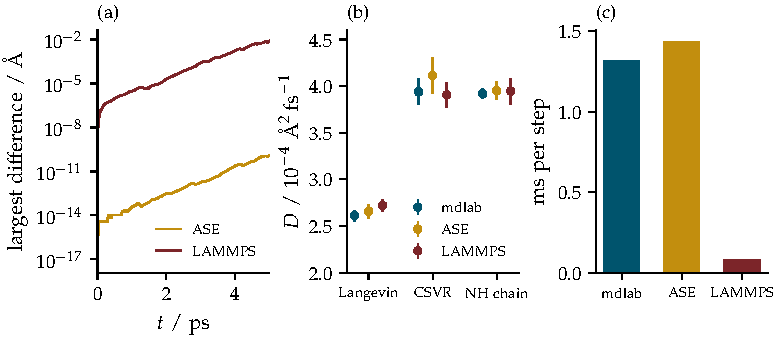
\includegraphics{ch17_practice/codes}
\caption{Chapter~12's liquid argon, 256 atoms at \SI{135}{\kelvin}, in
three codes with one model. (a) The largest difference of any coordinate
from \texttt{mdlab}'s, at fixed energy from one start, for ASE and for
LAMMPS with its table. (b) The diffusion coefficient from the MSD over 2
to \SI{20}{\pico\second} of \SI{200}{\pico\second} runs under Langevin
friction of \SI{1}{\per\pico\second}, CSVR and a Nosé-Hoover chain, with
time constants of \SI{1}{\pico\second}, and its standard error from five
blocks. (c) The time of one step of \SI{10}{\femto\second}.}
\label{fig:ip-codes}
\end{figure}

\begin{keyidea}
ASE holds atoms in one object and plugs any energy-and-force program into
it as a calculator, so its integrators, thermostats and barostats serve
every model. Its unit of time is \SI{10.18}{\femto\second}, and its cell
is the transpose of \texttt{mdlab}'s. With the same model the two codes
give the same trajectory until chaos amplifies their rounding, and the
same temperatures and diffusion coefficients.
\end{keyidea}

\notebook{17}{run one liquid in mdlab and in ASE and compare the paths}

\begin{selfcheck}
An ASE script sets \texttt{timestep=2} without \texttt{units.fs}. What step
does the run take, in femtoseconds?
\end{selfcheck}

%=============================================================================!
% 17.2  LAMMPS                                                                !
%=============================================================================!
\section{LAMMPS}
\label{sec:ip-lammps}

A player piano plays from a punched roll: each row of holes is a command,
read in order, and the piano does the rest at its own speed. LAMMPS, the
molecular dynamics code of Sandia National Laboratories\cite{Thompson2022},
is driven the same way, by an input script whose lines are commands read
in order, and it runs them in compiled C++ spread over many processors.
It is one of the codes most used for large classical and
learned-potential runs. This section reads an input script line by line, sets out the
units it works in, and runs the liquid of \cref{sec:ip-ase} in it.

\subsection*{An input script}

The commands that the runs of \cref{fig:ip-codes} pass to LAMMPS for the
liquid under CSVR are, with the steps written as one \texttt{run} (the
Python script takes them ten at a time, to read the positions between),
\begin{code}[language={},morecomment={[l]\#}]
units metal
atom_style atomic
atom_modify map array
read_data argon.data
pair_style table linear 20001
pair_coeff 1 1 argon.table ARGON 8.5
timestep 0.01
fix 1 all nve
fix 2 all temp/csvr 135.0 135.0 1.0 17
thermo_style custom step pe ke
run 20000
\end{code}
\noindent \texttt{units metal} fixes the units of everything that
follows: lengths in \si{\angstrom}, energies in \si{\electronvolt}, masses
in grams per mole, which are numerically \si{\amu}, temperatures in
\si{\kelvin}, pressures in bars and times in picoseconds, so that
\texttt{timestep 0.01} is \SI{10}{\femto\second} and velocities are in
\si{\angstrom\per\pico\second}. \texttt{atom\_style atomic} declares
atoms that carry only a type, a position and a velocity, and
\texttt{atom\_modify map array} keeps a lookup from each atom's identity
number to its place in memory. \texttt{read\_data} reads the cell, the
masses, the positions and the velocities from a file that ASE writes
(\texttt{ase.io.write} with \texttt{format="lammps-data"},
\texttt{units="metal"}, \texttt{masses=True} and
\texttt{velocities=True}; without the last two the file holds neither).
\texttt{pair\_style} and \texttt{pair\_coeff} set the forces between atoms
of type 1 from the section \texttt{ARGON} of \texttt{argon.table}, cut
off at \SI{8.5}{\angstrom}, as the next subsection describes.
\texttt{fix} commands act on the atoms at every step: \texttt{nve} is
velocity Verlet, and \texttt{temp/csvr} rescales the velocities as CSVR
does, towards a target that runs from the first temperature to the
second over the run (here both \SI{135}{\kelvin}), with its time constant
in picoseconds and a seed for its random numbers. \texttt{thermo\_style} chooses what is printed,
and \texttt{run} takes the steps. \Cref{tab:ip-methods} lists the fix for
each method of the book.

\begin{table}[htb]
\centering
\small
\caption{The methods of Chapters~9, 13 and~14 in the three codes, with the
unit of each one's time parameter: $\gamma$ in \si{\per\femto\second} and
$\tau$ in \si{\femto\second} for \texttt{mdlab}; for ASE, $\tau$ in its
time unit and $\gamma$ in its reciprocal (written \texttt{tau * units.fs}
and \texttt{gamma / units.fs}); for LAMMPS, $\tau$ and the damping
$1/\gamma$ in picoseconds.}
\label{tab:ip-methods}
\begin{tabular}{@{}>{\raggedright\arraybackslash}p{0.16\linewidth}
   >{\raggedright\arraybackslash}p{0.24\linewidth}
   >{\raggedright\arraybackslash}p{0.24\linewidth}
   >{\raggedright\arraybackslash}p{0.24\linewidth}@{}}
\toprule
method & \texttt{mdlab} & ASE & LAMMPS\\
\midrule
velocity Verlet & \texttt{md.run} & \texttt{VelocityVerlet} &
\texttt{fix nve}\\
Langevin & \texttt{thermostats.\allowbreak Langevin}, $\gamma$ & \texttt{Langevin},
friction $\gamma$ & \texttt{fix langevin}, damping $1/\gamma$, with
\texttt{fix nve}\\
CSVR & \texttt{thermostats.\allowbreak CSVR}, $\tau$ & \texttt{Bussi}, \texttt{taut} &
\texttt{fix temp/csvr}, with \texttt{fix nve}\\
Nosé-Hoover chain & \texttt{thermostats.\allowbreak NoseHoover\allowbreak Chain}, $\tau$ &
\texttt{NoseHoover\allowbreak ChainNVT}, \texttt{tdamp} & \texttt{fix nvt}\\
Berendsen & \texttt{thermostats.\allowbreak Berendsen}, $\tau$ & \texttt{NVTBerendsen},
\texttt{taut} & \texttt{fix temp/berendsen}, with \texttt{fix nve}\\
MTK piston & \texttt{barostats.\allowbreak run\_mtk} & \texttt{Isotropic\allowbreak MTKNPT},
\texttt{pdamp} & \texttt{fix npt \dots\ iso}\\
lengths apart & \texttt{barostats.\allowbreak Stochastic\allowbreak Cell\allowbreak Rescaling} &
\texttt{MaskedMTKNPT}, \texttt{mask} & \texttt{fix npt \dots\ aniso}\\
\bottomrule
\end{tabular}
\end{table}

\subsection*{The model as a table}

LAMMPS has its own Lennard-Jones forms, each with its own way of ending at
the cutoff, and a comparison of codes needs the model itself. Any pair
potential can be given as a table: \texttt{mdlab.io.lammps\_table} writes
$\varphi(r)$ and the force $F = -\dd\varphi/\dd r$ at \num{20001} equally
spaced distances from 0.5 to \SI{8.5}{\angstrom}, \SI{4e-4}{\angstrom}
apart. LAMMPS does not interpolate these points as they stand: it passes a
smooth curve, a spline, through them and reads from it its own table of
\num{20001} entries equally spaced in $r^2$,
\SI{0.0036}{\angstrom\squared} apart, and \texttt{pair\_style table
linear} interpolates $F/r$ along straight lines in $r^2$ between those.
Interpolating a function $y$ along a straight line between points a
distance $\delta x$ apart misses it by at most $\delta x^2\max\lvert
y''\rvert/8$ (\cref{ex:ip-table}). Measured from the midpoint, the
parabola $y = \frac12 y''x^2$ has the height $\frac12 y''(\delta x/2)^2$
at both ends, so the chord is the flat line at that height, and at the
midpoint, where the parabola is at zero, the two part by $\frac12
y''(\delta x/2)^2 = \delta x^2 y''/8$. Here $y$ is $F/r$ and $x$ is $r^2$.
Near \SI{3}{\angstrom}, about the closest that atoms of the liquid come
(\SI{2.98}{\angstrom} in \texttt{mdlab}'s \SI{200}{\pico\second} under
CSVR), a step of \SI{0.0036}{\angstrom\squared} in $r^2$ is
$0.0036/(2\times3) = \SI{6e-4}{\angstrom}$ in $r$, and the largest miss of
the force beyond \SI{3}{\angstrom}, found by placing a pair of atoms at
the midpoint of every interval of LAMMPS's table, is
\SI{7.6e-7}{\electronvolt\per\angstrom}, \num{1.3e-6} of the force there,
and the run shows it. At fixed energy LAMMPS's energy spreads by the same
\SI{0.469}{\milli\electronvolt} as \texttt{mdlab}'s, but its positions
part from \texttt{mdlab}'s by \SI{3.0e-6}{\angstrom} after
\SI{1}{\pico\second}, against ASE's \num{3.9e-14}, and by
\SI{7.8e-3}{\angstrom} after \SI{5}{\pico\second} (\cref{fig:ip-codes}a):
the table's small error is a difference like any other, and the chaos
amplifies it.

\subsection*{Temperatures and diffusion}

Under the same three thermostats, given as \texttt{fix langevin},
\texttt{fix temp/csvr} and \texttt{fix nvt}, LAMMPS's runs reach mean
temperatures within three errors of \SI{135}{\kelvin} and spreads of
0.962 to 0.996 of the canonical, and its diffusion coefficients lie
within 1.2 combined errors of the other codes' (\cref{fig:ip-codes}b). An
option of \texttt{fix langevin} may matter as well. Over
\SI{1}{\nano\second}, $D$ is $(2.721 \pm 0.038)\times10^{-4}$\,\si{\angstrom
\squared\per\femto\second} in LAMMPS and $(2.681 \pm 0.023)\times10^{-4}$
in \texttt{mdlab}, 0.9 combined errors apart; with \texttt{zero yes},
which removes the sum of the random forces at every step so that they
cannot push the centre of mass, LAMMPS gives $(2.806 \pm
0.021)\times10^{-4}$, 2.0 combined errors above its own value without the
option and 4.0 above \texttt{mdlab}'s. The option's own effect, two
combined errors, is at the edge of what these runs can resolve, and a run that reports transport under a local thermostat should
state such options with the friction; the transport coefficients of
\cref{sec:ob-trajectory} belong in any case to runs at fixed energy or
under a global thermostat.

LAMMPS takes \SI{0.08}{\milli\second} a step for these 256 atoms, a
sixteenth of \texttt{mdlab}'s \SI{1.32}{\milli\second}: compiled C++
throughout, against \texttt{mdlab}'s NumPy and Numba
(\cref{sec:md-speed}).

\subsection*{Python and LAMMPS}

LAMMPS can also be driven from Python, through its module \texttt{lammps}:
\texttt{commands\_\allowbreak string} passes lines of a script,
\texttt{extract\_\allowbreak atom} returns the positions, velocities,
forces and other arrays of the atoms, and \texttt{get\_thermo} any printed
quantity. Two details of those arrays trip up a reader. LAMMPS wraps
positions into the cell and keeps, for each atom, an image flag: the net
number of cells it has crossed along each axis, a crossing back counting
minus one, so that the unwrapped position is the wrapped one plus the
flags times the lattice vectors. And LAMMPS reorders its atoms in memory
every thousand steps, to keep neighbours near one another, so the arrays
must be read in the order of their identity numbers,
\texttt{extract\_\allowbreak atom("id")}, at every frame;
\cref{sec:ip-trajectory} measures what happens when they are not. The same
module lets LAMMPS call Python for its forces, which the next section
uses.

\begin{keyidea}
LAMMPS runs an input script of commands in order, in \texttt{metal} units
with times in picoseconds. Thermostats and barostats are fixes, any pair
potential can be a table, and its Python module reads and sets the atoms'
arrays, in the order of their identities. With the same model it gives
the same energies, temperatures and diffusion coefficients as
\texttt{mdlab} and ASE, at a sixteenth of the time per step.
\end{keyidea}

\notebook{17}{write a LAMMPS input from Python and check its forces}

\begin{selfcheck}
A LAMMPS script in \texttt{metal} units sets \texttt{timestep 1.0}. What is
the step in femtoseconds, and what would it do to liquid argon?
\end{selfcheck}

%=============================================================================!
% 17.3  A LEARNED POTENTIAL IN BOTH                                           !
%=============================================================================!
\section{A learned potential in both}
\label{sec:ip-learned}

A translator who has read millions of sentences can render one never
seen before, but only in the languages that reading covered, and the
gaps in a translation show where the reading was thin. A foundation
model of interatomic forces, one trained once on a wide range of
materials to be used on any of them, is in the same position.
MACE-MP-0\cite{Batatia2025} is a network of the kind that the planned continuation of Part~V builds,
trained on the calculations of the Materials Project\cite{Deng2023},
compounds of 89 elements, at every structure each calculation passed
through on its way to its least energy. They use density-functional
theory (\cref{sec:pe-origin}), which needs an approximation, called the
functional, for one part of the electrons' energy; theirs is
PBE\cite{Perdew1996}, with an added correction for the oxides and
fluorides of some transition metals. The model gives energies and forces
for structures it was never shown. This section runs it in ASE
and in LAMMPS, measures what it costs, finds one of its gaps, and chooses
the time step for lithium in graphite.

\subsection*{Running it}

In ASE the model is a calculator like any other: MACE's package provides
one that loads the trained weights, \texttt{mace\_mp}. It runs on the
computer's main processor, the CPU, here on five of its cores at once
(five threads), or on its graphics processor, the GPU, a chip of many
small cores that do the same arithmetic on many numbers at once; and it
keeps its numbers in double precision (float64), the 16 significant
digits of \cref{sec:pe-forces}, or in single precision (float32), about
7. The GPU of the machine used here, an Apple M5 Pro, holds no
double-precision numbers, and the
version of the package used, 0.3.16, stores the energy of each atom in
double precision; the chapter's scripts keep that one output in single
precision on the GPU, which leaves the forces untouched, and check the
result against double precision on the CPU.

LAMMPS runs MACE's own pair styles only when it is built with extra
packages for them, which its standard distribution lacks. Its Python
module offers another way in: the command \texttt{fix ext all external
pf/callback 1 1} makes LAMMPS call a Python function at every step with
the positions, and the forces that function returns are added to the
atoms', its energy to the run's. The function builds an ASE \texttt{Atoms}
from LAMMPS's positions and cell and asks MACE for the forces. On a cell
of 56 atoms of LiC$_6$, eight copies of the seven-atom cell of
\cref{sec:ip-lic6}, moved at random by about \SI{0.05}{\angstrom},
LAMMPS's energy equals ASE's to the last of nine digits, and its forces
equal ASE's to \SI{1.4e-13}{\electronvolt\per\angstrom} once one detail is
handled: LAMMPS holds every cell with its first lattice vector along
$x$ and its second in the $xy$ plane, so ASE turns this cell to fit when
it writes LAMMPS's data file, and a comparison of forces must be made
with the cell as LAMMPS holds it.

\subsection*{A gap: dispersion}

The weak attraction between the sheets of graphite comes from the
correlated motion of their electrons, dispersion, which PBE leaves out.
A model trained on PBE inherits the gap. Graphite's cell holds two
sheets, and its height $c$ is twice their spacing. With MACE-MP-0 alone,
graphite's energy is least at $c = \SI{7.818}{\angstrom}$, 16.5\% above
Trucano and Chen's \SI{6.711}{\angstrom}\cite{TrucanoChen1975}, and
stretching the cell to $c = \SI{9}{\angstrom}$, the sheets
\SI{4.5}{\angstrom} apart, costs only \SI{5.2}{\milli\electronvolt} per
atom (\cref{fig:ip-learned}c). Grimme's D3 correction\cite{Grimme2010}
adds an attraction for every pair of atoms, falling as $1/r^6$ and
$1/r^8$, with coefficients from reference calculations for the 94
elements from hydrogen to plutonium; Becke--Johnson
damping\cite{Grimme2011} keeps it finite where atoms come close. With it
the least energy lies at \SI{6.612}{\angstrom}, 1.5\% below the measured
value, with a binding of \SI{41.2}{\milli\electronvolt} per atom against
$c = \SI{9}{\angstrom}$. Relaxed with the correction, graphite's in-plane
constant is \SI{2.4647}{\angstrom}, 0.03\% above Trucano and Chen's
\SI{2.464}{\angstrom}. The correction is added in ASE by summing its
calculator with MACE's, and it costs \SI{12}{\milli\second} for 126
atoms on the CPU, a twentieth of the medium model's call on the GPU. Every run below includes it.

\subsection*{What it costs}

MACE-MP-0 comes in sizes; the medium model takes \SI{1.20}{\second} for
one call on 126 atoms on five CPU threads in double precision,
\SI{0.62}{\second} in single precision, and \SI{0.25}{\second} on the GPU,
and the small model \num{0.40}, \num{0.21} and \SI{0.081}{\second}
(\cref{fig:ip-learned}a). Every setting grows nearly in proportion to
the number of atoms from 28 to 1008, as the neighbour list makes each
atom's work local, though on the GPU the cost per atom rises by 40\% from
252 to 1008 atoms; for the medium model the GPU is 1.9 to 2.7 times
faster than the CPU in single precision, and 3.5 to 4.8 times faster than
in double. Against the \SI{0.08}{\milli\second} that LAMMPS takes for a step
of 256 argon atoms (\cref{sec:ip-lammps}), a learned potential is
thousands of times dearer per atom, and cheap only beside the electronic
structure it replaces (\cref{sec:ip-aimd}).

\subsection*{The time step}

The test of \cref{sec:in-stability} chooses the step. LiC$_6$, 56 atoms,
was started from velocities drawn at \SI{600}{\kelvin} and run for
\SI{2}{\pico\second} at fixed energy with steps of 0.5, 1, 2 and
\SI{3}{\femto\second} in double precision (\cref{fig:ip-learned}b). The
spread of the total energy is 0.0017, 0.0067, 0.028 and 0.082 of the
kinetic energy's, growing between the shorter steps by 4.02 and 4.16,
against the 4 of $\dt^2$, and from 2 to \SI{3}{\femto\second} by 2.92,
against 2.25: at the longest step the growth outruns $\dt^2$. The mean
total energy of the last quarter of each run differs from that of the
first by less than \SI{0.1}{\milli\electronvolt} up to
\SI{2}{\femto\second}, and by \SI{17.6}{\milli\electronvolt} at
\SI{3}{\femto\second}. Single precision on the GPU gives the same spreads
and the same small differences at 1 and \SI{2}{\femto\second}, so for this
system its rounding is harmless. The longest step that passes is
\SI{2}{\femto\second}; the runs below take \SI{1}{\femto\second}, a
margin for runs of tens of picoseconds at up to \SI{600}{\kelvin}.

\begin{figure}[htb]
\centering
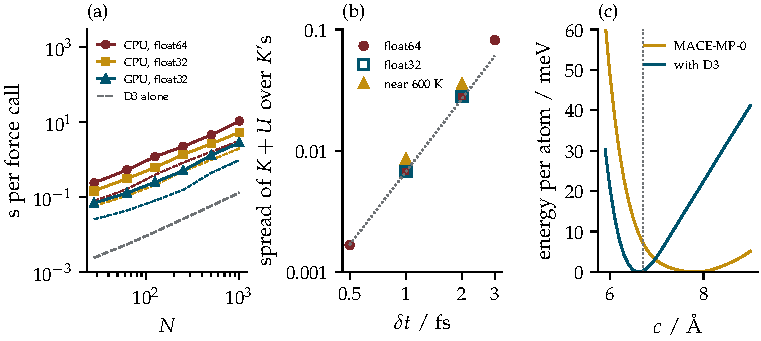
\includegraphics{ch17_practice/learned}
\caption{MACE-MP-0 with D3. (a) The time of one force call against the
number of atoms, LiC$_6$ cells of 28 to 1008 atoms, for the medium model
(solid) and the small (dashed) on five CPU threads in double and single
precision and on the GPU in single precision, and for D3 alone (grey). (b)
LiC$_6$, 56 atoms, at fixed energy: the spread of the total energy over
that of the kinetic energy against the step, in double (circles) and
single (squares) precision near \SI{245}{\kelvin}, and in double
precision near \SI{600}{\kelvin} (triangles), with lines $\propto\dt^2$
through \SI{1}{\femto\second} (dotted). (c) Graphite's energy against the length
$c$ of its cell, with MACE-MP-0 alone and with D3, against the measured
$c$ (dotted).}
\label{fig:ip-learned}
\end{figure}

\begin{keyidea}
A foundation model runs as an ASE calculator, and in LAMMPS through a
Python callback, with the same forces. It inherits the gaps of its
training functional, here dispersion, which D3 restores. It costs about
a quarter of a second per call for a hundred atoms on a GPU, growing
nearly in proportion to the number of atoms, and its time step is chosen by the
same test at fixed energy as any other model's.
\end{keyidea}

\notebook{17}{switch D3 on and off and watch graphite's sheets}

\begin{selfcheck}
A learned potential trained only on bulk metals is used for a metal
surface covered by water. Which part of the system needs checking first,
and how?
\end{selfcheck}

%=============================================================================!
% 17.4  FIRST-PRINCIPLES MOLECULAR DYNAMICS AND ITS COST                      !
%=============================================================================!
\section{First-principles molecular dynamics and its cost}
\label{sec:ip-aimd}

A map drawn from a survey is only as good as the survey, and a survey of
every field is too costly to repeat for each journey; the map is drawn
once and then used. A learned potential is such a map, and the survey is
electronic-structure theory, which gives the energy and forces of atoms
from their electrons (\cref{sec:pe-origin}). Molecular dynamics with
those forces at every step, first-principles or \emph{ab initio}
molecular dynamics, needs no fitted potential, and it is what a learned
potential is trained to imitate. This section measures what it costs,
with FHI-aims\cite{Blum2009}, which describes each electron's wave as a
sum of functions centred on the atoms, stored as tables of numbers, and
can run molecular dynamics itself.

\subsection*{One frame of LiC$_6$}

The 28 atoms of a $2\times2\times1$ cell of LiC$_6$, four copies of the
seven-atom cell of \cref{sec:ip-lic6}, taken from a run of MACE-MP-0 at
\SI{300}{\kelvin}, were given to FHI-aims with the PBE functional and its
standard `light' settings, the cheapest of its standard choices of basis
functions and integration grids, on four cores of an Apple M1 Max, once
for each of the three grids below. The electrons are found by a
self-consistent iteration: the potential each electron feels depends on
the density of all of them, the number per unit volume at each point,
which is built from their waves, which are in turn set by the potential;
so each cycle builds a potential from the density and a density from the
potential, until neither changes. This frame needed 16 or 17 cycles,
\SI{337}{\second} to \SI{385}{\second} in all: 14 to \SI{16}{\second} for
each ordinary cycle and 57 to \SI{60}{\second} for each of the last two,
which also computed the forces. A step of molecular dynamics starts from
the density of the step before, extrapolated, and needs fewer cycles. If
it took half the time of this calculation from scratch, an estimate that
a short run would test, a step would cost about \SI{192}{\second}, and a
picosecond of steps of \SI{1}{\femto\second} about \SI{53}{\hour} on these
four cores; the two cycles with forces do not shrink, so this is the
cheaper end. MACE-MP-0 with D3 takes \SI{214}{\milli\second} a step of
molecular dynamics for the same cell on the same machine's GPU, with other
runs sharing the machine, about 900 times less (and
\SI{72}{\milli\second} a call alone on the faster machine of
\cref{fig:ip-learned}a). The gap widens with size, since the cost of the
electronic structure grows faster than the number of atoms
(\cref{sec:pe-origin}).

\subsection*{A setting to converge}

LiC$_6$ is a metal. In a crystal each electron's wave repeats from one
cell to the next up to a shift of its phase, and the code finds the
electrons separately for each of a grid of such shifts, the $k$-points,
and averages over them; a metal, whose filled energy levels end
abruptly, needs a fine grid. A grid of $4\times4\times10$ shifts along
the three cell vectors has 160 points, but a shift and its reverse give
the same energies, which leaves 84 to compute; grids of $2\times2\times5$
and $3\times3\times8$ leave 12 and 37. The forces on the carbon atoms of
this frame, up to \SI{3.1}{\electronvolt\per\angstrom}, change by up to
\SI{0.16}{\electronvolt\per\angstrom} between the grids of 12 and 84
points and by up to \SI{0.28}{\electronvolt\per\angstrom} between those
of 37 and 84: they have not settled by 37 points, nothing yet shows that
they have by 84, and a denser grid is needed before these frames can
serve as a reference. A reference
calculation is converged in its own settings before anything is compared
with it, as a molecular dynamics run is converged in its time step
and length.

\subsection*{What is left to check}

The lithium studies of the next two sections rest on MACE-MP-0, and no
calculation here has yet compared its forces, or its barrier for a
lithium hop, with PBE for this system. Their numbers are therefore the
model's predictions. The check, single points at a converged grid on
frames of the runs and along lithium's paths between sites, is the first
step of the protocol of \cref{sec:ip-protocol} for any learned potential,
and the planned continuation of Part~V returns to it when it trains a model of its own on these data.

\begin{keyidea}
First-principles molecular dynamics computes the electrons at every step
and needs no fitted potential, at a cost of minutes a step for a few
dozen atoms, on this estimate about nine hundred times a foundation
model's here. Its settings,
such as the grid of $k$-points of a metal, are converged before it serves
as a reference, and a learned potential is checked against it on the
system at hand before its predictions are trusted.
\end{keyidea}

\notebook{17}{read the cost of a first-principles step and of a learned one}

\begin{selfcheck}
A first-principles step of 28 atoms costs \SI{192}{\second}. If the cost
grew as the cube of the number of atoms, as it does once finding the
eigenvectors dominates (\cref{sec:pe-origin}), roughly how long would a
step of 112 atoms take?
\end{selfcheck}

%=============================================================================!
% 17.5  LiC6 WITH A FOUNDATION MODEL                                          !
%=============================================================================!
\section{\texorpdfstring{LiC$_6$}{LiC6} with a foundation model}
\label{sec:ip-lic6}

Books pushed between the shelves of a bookcase whose shelves can slide
force them apart, while the shelves themselves keep their length. Lithium
does this to graphite. Chapter~14 could only imitate it with a model solid
(\cref{sec:pr-shape}); with MACE-MP-0 and D3 the real material can be
run, and this section does so for the fully lithiated compound LiC$_6$ at
room temperature, the study that Chapters~13 and~14 left for a real
potential. Its numbers are the model's predictions (\cref{sec:ip-aimd}).

\subsection*{Building the cells}

ASE builds the structures. Graphite's cell holds four atoms, two in each
of its sheets stacked A, B, with Trucano and Chen's lattice constants as
the start. In LiC$_6$ the sheets stack A, A and a lithium atom sits over
every third hexagon, the pattern written
$\sqrt3\times\sqrt3$\,R30$^\circ$: its cell is the sheet's own cell made
$\sqrt3$ times longer and turned by \ang{30}, built in ASE as the
supercell of the two-atom cell of graphene, a single sheet of graphite,
whose vectors $\vb{a}$ and $\vb{b}$ have length $a$ and lie \ang{120}
apart, with the vectors $2\vb{a} + \vb{b}$ and $-\vb{a} + \vb{b}$
(\cref{ex:ip-supercell}), and it holds six carbon atoms and one lithium.
Relaxed together with its cell at \SI{0}{\kelvin}, to forces below
\SI{1}{\milli\electronvolt\per\angstrom} and stresses below
\SI{0.02}{\giga\pascal}, LiC$_6$'s sheets lie \SI{3.616}{\angstrom} apart,
2.3\% below the measured \SI{3.70}{\angstrom} quoted by Hazrati, de Wijs
and Brocks\cite{Hazrati2014}, and the sheet's lattice constant $a$, the
side of its two-atom cell, is \SI{2.4864}{\angstrom}, 0.88\% longer than
the \SI{2.4647}{\angstrom} of graphite relaxed with the same model: the
sheets stretch a little, as the electrons that lithium gives them are
expected to make them do.

\subsection*{Anisotropic and isotropic coupling at \SI{300}{\kelvin}}

A cell of $3\times3\times1$ of these units, 63 atoms, was run at
\SI{300}{\kelvin} and zero pressure with ASE's \texttt{MaskedMTKNPT}, which
lets each lattice vector change its length while keeping its direction,
with $\tau_{\mathrm T} = \SI{100}{\femto\second}$ and $\tau_{\mathrm P} =
\SI{1}{\pico\second}$, for \SI{20}{\pico\second}; and with
\texttt{IsotropicMTKNPT}, which scales the three lengths together, for
\SI{10}{\pico\second} (\cref{fig:ip-lic6}). The isotropic run keeps the
ratio of the lengths it started from, and the stiff sheets hold the
in-plane length, and with it the spacing, at their values at
\SI{0}{\kelvin}: the spacing stays at $(3.6162 \pm
0.0005)$\,\si{\angstrom}. The diagonal of the pressure tensor, computed
from the model's stress with the atoms' kinetic part added, on 25 frames
of the last \SI{5}{\pico\second}, is $(-1.00 \pm 0.45)$, $(-1.11 \pm
0.36)$ and $(1.68 \pm 0.10)$\,\si{\giga\pascal} along $x$, $y$ and $z$:
the sheets push apart along $z$ while each sheet pulls in along $x$ and
$y$, and only the mean is zero. With the lengths coupled apart, all
three components, from 75 frames of the last \SI{15}{\pico\second}, are
zero within 1.2 of their errors, $(0.06 \pm 0.28)$, $(-0.21 \pm 0.18)$
and $(0.01 \pm 0.06)$\,\si{\giga\pascal}, and the spacing opens on
warming.

\subsection*{How long the spacing takes}

The in-plane length settles at once: over the \SI{20}{\pico\second} the
lattice constant $a$ is $(2.4836 \pm 0.0004)$\,\si{\angstrom}, its
quarters agreeing to \SI{0.001}{\angstrom}; \texttt{convergence\_report}
flags it only because its blocks give a smaller error,
\SI{0.0002}{\angstrom}, than the one quoted. The spacing does not settle. Its
means over the four quarters of the run are 3.756, 3.760, 3.766 and
\SI{3.778}{\angstrom}, still rising, and \texttt{convergence\_report}
refuses it with 82 independent samples, fewer than the 100 that the
criterion of \cref{sec:cv-protocol} asks. A layered solid's soft
direction relaxes slowly. These saved results do not yet establish its
equilibrium spacing; a longer run is required.

\begin{figure}[htb]
\centering
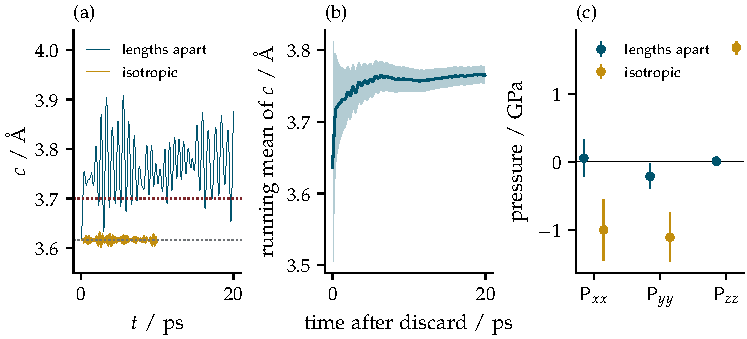
\includegraphics{ch17_practice/lic6}
\caption{LiC$_6$, 63 atoms, at \SI{300}{\kelvin} and zero pressure with
MACE-MP-0 and D3. (a) The spacing of the sheets against time with the
lattice lengths coupled apart (teal) and together (ochre), with the
relaxed spacing at \SI{0}{\kelvin} (grey dotted) and the measured
\SI{3.70}{\angstrom} (red dotted). (b) The running mean of the spacing in
the initial \SI{20}{\pico\second} from the start that
\texttt{convergence\_report} finds,
with twice its error (band). (c) The diagonal of the pressure tensor
under each coupling, with its standard error.}
\label{fig:ip-lic6}
\end{figure}

\begin{keyidea}
A foundation model with D3 relaxes LiC$_6$ to within a few per cent of
its measured spacing, and runs it at room temperature. A layered solid
needs its lattice lengths coupled apart: coupled together, the spacing is
held and the diagonal of the pressure tensor shows the strain. Its soft
direction relaxes over tens of picoseconds, and the convergence report
decides when it has settled.
\end{keyidea}

\notebook{17}{couple LiC6's lengths together and apart, and watch the spacing}

\begin{selfcheck}
In LiC$_6$, how many hexagons of a sheet are there for each lithium atom,
and why does that give six carbon atoms?
\end{selfcheck}

%=============================================================================!
% 17.6  LITHIUM ON THE MOVE                                                   !
%=============================================================================!
\section{Lithium on the move}
\label{sec:ip-hops}

A marble in an egg box that is being shaken rattles in its cup and now
and then jumps into the next. Counting its jumps needs two decisions:
what a cup is, and how long the marble must stay in a new cup for the
visit to count, since a marble that touches the rim of a neighbour and
falls back has gone nowhere. If the egg box itself slides about on the
table, the cups move with it, and the marble's cup must be read in the
frame of the box. A lithium atom in a gallery of graphite, the gap
between two neighbouring sheets, is such a marble. This section counts its hops in dilute graphite, one lithium
among 64 carbon atoms, and turns them into rates with error bars, taking
Chapter~13's hops over a model surface (\cref{sec:th-langevin}) and
Chapter~16's counting of events (\cref{sec:ob-reactions}) to a real
material.

\subsection*{The sites}

Relaxed at \SI{0}{\kelvin}, lithium sits over the centre of a hexagon of
the sheet below, a hollow, and under an atom of the sheet above, since in
graphite's A, B stacking a hollow of one sheet lies under an atom of the
next. Graphite has an inversion centre midway between an atom of the
sheet below and the atom of the sheet above that lies over it: sending
every point to the point as far beyond that centre on the opposite side
swaps the two sheets and leaves the crystal as it was. It carries
lithium's site to one over an atom of the sheet below, a corner of
lithium's hexagon, and under a hollow of the sheet above: a second family
of sites with the same energy, $a/\sqrt3 = \SI{1.42}{\angstrom}$ from the
first, for the lattice constant $a = \SI{2.4648}{\angstrom}$ of the
relaxed dilute cell. Each family is the hollows of one sheet, a
triangular grid, and the two grids are offset by $a/\sqrt3$, so together
they form a honeycomb on which the families alternate, as the two kinds
of atom of a sheet do (\cref{ex:ip-honeycomb}).

Moved along the straight line to the nearest site of the other family,
with its position in the plane held at each of eight steps while its
height and the carbon atoms relax, lithium's energy rises to
\SI{73}{\milli\electronvolt} halfway and falls back to zero at the far
site, as the inversion requires; along the line to the next site of its
own family, across the middle of a C--C bond, it rises to
\SI{107}{\milli\electronvolt} (\cref{fig:ip-hops}a). Without D3, at the
same relaxed points, the two are 53 and \SI{94}{\milli\electronvolt}. One
carbon atom of each sheet is held in the plane as well, since otherwise
the sheets would slide to carry their sites back under lithium. Every
path between two sites must cross the ridge that divides them, whose
lowest point, the saddle, sets the barrier (\cref{sec:en-gradient}), so
the highest point of any one path is at least the barrier, and
\SI{73}{\milli\electronvolt} bounds it from above. The relaxation of the
carbon atoms is part of every site. With them held where they relaxed
around the first site, the other family's site lies
\SI{136}{\milli\electronvolt} higher and is no minimum at all, the
straight way to it passing 56, 123 and \SI{111}{\milli\electronvolt}, so
a map over a frozen host finds only half the sites.

\subsection*{Sheets that slide}

Each run, at 300, 450 and \SI{600}{\kelvin}, lasted \SI{20}{\pico\second}
under CSVR with $\tau_{\mathrm T} = \SI{1}{\pico\second}$ and steps of
\SI{1}{\femto\second}, keeping lithium's position every
\SI{10}{\femto\second} and every atom's every \SI{100}{\femto\second}.
The cell was the one relaxed at \SI{0}{\kelvin}, held fixed, which at
these temperatures holds the sheets closer than zero pressure would, as
LiC$_6$'s pressure along $c$ in its own cell showed (\cref{sec:ip-lic6});
the rates below belong to that cell. In them the sheets slide as wholes. The sheet
below lithium slides by as much as 0.96, 2.40 and \SI{1.59}{\angstrom},
and the sheet above by as much as 1.94, 4.76 and \SI{2.97}{\angstrom}
against it, comparable with or further than the \SI{1.42}{\angstrom}
between neighbouring sites, so a site fixed in the frame of the cell is
soon in the wrong place. Each family is the hollows of one sheet, the
first those of the sheet below and the second those of the sheet above.
Lithium's position is therefore read in the frame of each sheet in turn,
the sheet's slide being the mean displacement of its atoms, interpolated
between the frames that hold them, and lithium is assigned to the
nearest site of either family. Sites fixed in the cell where the sheets
started give a count of hops that falls steadily as the least stay of the
next subsection grows, from 85 to 20 at \SI{450}{\kelvin}.

How far the sheets wander is a property of the small cell. Near its best
stacking, sliding a sheet of $N$ atoms by $s$ along one direction costs
about $\frac12N\kappa s^2$, with $\kappa$ the stiffness for one atom,
since every atom of the sheet changes its stacking at once; equipartition
gives this term $\frac12\kB T$ on average whatever $N$
(\cref{sec:sm-equipartition}). The typical slide, $\sqrt{\kB T/N\kappa}$,
therefore shrinks as the sheet grows, and the barrier between one
stacking and the next, $N$ times that for one atom, grows. A sheet of 32
atoms wanders much further than the sheets of a crystal, and a larger
cell is the test of how much of what follows depends on it
(\cref{sec:cv-size}).

\subsection*{Counting hops}

The runs start from the relaxed cell with velocities drawn at the target,
and half the kinetic energy passes at once into the potential energy, as
in the crystal of \cref{sec:sm-trajectory}: the first picosecond averages
200, 301 and \SI{402}{\kelvin}. The test of \cref{sec:cv-equilibration}
on the kinetic temperature finds the start at 2.5, 2.5 and
\SI{7.6}{\pico\second}, after which the runs average 298, 447 and
\SI{592}{\kelvin}, and hops are counted from there, over 17.5, 17.5 and
\SI{12.4}{\pico\second}.

A visit counts only if it lasts a least stay, the same device as the
least lifetime of a bond (\cref{sec:ob-bonds}); a shorter visit is joined
to the one before it. With both families of sites the count barely
depends on the least stay up to \SI{50}{\femto\second}: 14, 14, 12 and
12 hops at \SI{300}{\kelvin}, 45, 43, 43 and 42 at 450 and 44, 43, 42
and 42 at \SI{600}{\kelvin}, for least stays of 10, 20, 30 and
\SI{50}{\femto\second} (\cref{fig:ip-hops}b). Beyond, the least stay
begins to discard visits that were real, most at \SI{600}{\kelvin}, where
a visit lasts \SI{0.30}{\pico\second} on average. With the sites of the
sheet below alone the count keeps falling at \SI{300}{\kelvin}, from 28
at a least stay of \SI{10}{\femto\second} to 8 at
\SI{200}{\femto\second}: a position over a site of the other family is
equally far from three sites of the first, and the jitter shares it out
among them, each change a hop. A count that falls steadily as the least
stay grows is the sign of a wrong definition of a site; a plateau is the
sign of a right one, and the least stay is chosen on it, here
\SI{50}{\femto\second}. The hops then join the two families, all of them
at \SI{300}{\kelvin}, 98\% at 450 and 95\% at \SI{600}{\kelvin}, as hops
between neighbours on the honeycomb must; the few others join two sites
of one family, the visit between them having been shorter than the least
stay.

Bonds would not have served. The bond tracker of \cref{sec:ob-bonds},
with its thresholds of 2.45 and \SI{2.86}{\angstrom} for lithium and
carbon, finds lithium bonded to ten carbon atoms in half the frames at
\SI{300}{\kelvin} and to nine in 45\%: the six of the hexagon on one
side, \SI{2.30}{\angstrom} away at \SI{0}{\kelvin}, the atom opposite,
\SI{2.08}{\angstrom}, and that atom's three neighbours,
\SI{2.45}{\angstrom}, on the threshold at which a bond forms. Those three
flicker in and out with the vibrations, each flicker an event of the
tracker, while a hop only exchanges which sheet holds the six and which
the four. The sites count the hops; the bonds would count the
vibrations.

\subsection*{Rates}

With a least stay of \SI{50}{\femto\second} the runs hold 12, 42 and 42
hops. A rate from $n$ events is known to $1/\sqrt n$
(\cref{sec:ob-reactions}), and we call a rate resolved at a fifth, which
needs 25 of them: at \SI{450}{\kelvin} the rate is $(2.40 \pm
0.37)$\,\si{\per\pico\second} and at \SI{600}{\kelvin} $(3.38 \pm
0.52)$\,\si{\per\pico\second}, while at \SI{300}{\kelvin}, $(0.69 \pm
0.20)$\,\si{\per\pico\second} from 12 hops, it is unresolved, and a run of
\SI{36}{\pico\second} in all at that rate would resolve it. The error
$\sqrt n$ assumes hops independent in time. Counted in ten equal windows
of each run, their variance is 1.3, 1.3 and 1.8 times their mean, against
$1 \pm 0.47$ for independent events (\cref{ex:cv-error-error}), within
twice that scatter, so the Poisson errors stand. Over the whole runs,
warming included, the ratios are 1.9, 2.2 and 2.3, beyond twice that
scatter at 450 and \SI{600}{\kelvin}: while a run warms its hops come in
bursts, one more reason to discard the start.

The logarithm of the rate against $1/\kB T$, each point weighted by $\sqrt
n$ as in \cref{sec:ob-reactions}, has the slope $-(80 \pm
17)$\,\si{\milli\electronvolt} (\cref{fig:ip-hops}c): the rate rises 4.9
times from 300 to \SI{600}{\kelvin}, where a barrier of
\SI{73}{\milli\electronvolt} would raise it $\mathrm{e}^{0.073\times(38.68
- 19.34)} = 4.1$ times, with $1/\kB T$ in \si{\per\electronvolt}. The
apparent activation energy lies above the bound from the relaxed path by
less than half its error, which at a fifth of its value is all that three
points, one of them unresolved, can give; a barrier from rates to a few
\si{\milli\electronvolt} needs more temperatures and many more hops at
each.

\begin{figure}[htb]
\centering
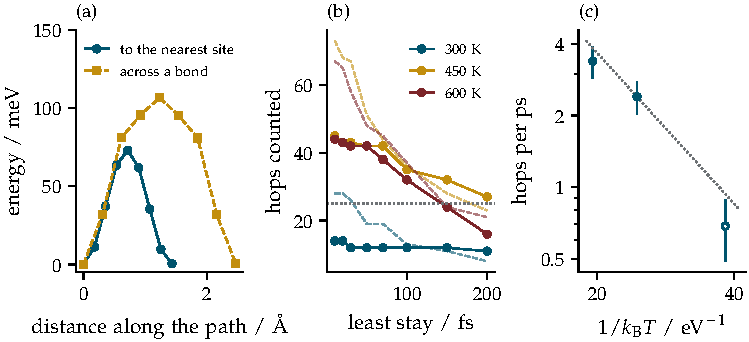
\includegraphics{ch17_practice/hops}
\caption{Lithium in dilute graphite, one lithium among 64 carbon atoms,
with MACE-MP-0 and D3. (a) The energy along the straight line to the
nearest site of the other family (teal) and to the next site of the
same family across a C--C bond (ochre), every atom relaxed but lithium
and one carbon of each sheet, whose positions in the plane are held.
(b) Hops counted after each run's start against the least stay a visit
needs to count, with the sites of both families (solid) and of the sheet
below alone (dashed), and the 25 hops that resolve a rate to a fifth
(dotted). (c) The rate of hops for a least stay of
\SI{50}{\femto\second}, with its Poisson error (open: unresolved),
against $1/\kB T$, with the line $\propto\mathrm{e}^{-E_{\mathrm a}/\kB
T}$ through the point at \SI{450}{\kelvin}, for $E_{\mathrm a}$ the
highest point of the teal path (dotted).}
\label{fig:ip-hops}
\end{figure}

\subsection*{Diffusion}

If each hop were independent of the last, the rate would give the
diffusion coefficient, $D = k_{\mathrm h}\ell^2/4$ with $\ell =
\SI{1.4231}{\angstrom}$ (\cref{ex:ip-honeycomb}): with $k_{\mathrm h} =
\num{2.40e-3}$ and \num{3.38e-3} per femtosecond, $D =
\num{2.40e-3}\times1.4231^2/4 =
\SI{12.2e-4}{\angstrom\squared\per\femto\second}$ at \SI{450}{\kelvin} and
\SI{17.1e-4}{\angstrom\squared\per\femto\second} at \SI{600}{\kelvin}.
Lithium's own mean squared displacement after the start, read in the
frame midway between the two sheets and fitted from 0.5 to
\SI{2}{\pico\second} in four blocks, gives $(5.8 \pm 2.2)$, $(22.4 \pm
16.0)$ and $(36.1 \pm 12.6)\times10^{-4}$\,\si{\angstrom\squared\per
\femto\second}, fractional errors of 0.38, 0.71 and 0.35, which miss a
target of 5\% by factors of seven to fourteen. Two
departures from the random walk are measured. The hops are not
independent: a hop returns to the site just left in $0.15 \pm 0.06$ of
cases at both 450 and \SI{600}{\kelvin}, errors $\sqrt{p(1-p)/m}$ for a
fraction $p$ of $m$ pairs of successive hops, three errors below the
$1/3$ of a random walk on the honeycomb, where the site just left is one
of three equally likely; at \SI{300}{\kelvin}, $0.27 \pm 0.13$, the
difference is within its error. Lithium therefore tends to carry on the
way it was going, and the correlation factor of \cref{sec:ob-layers}
exceeds 1, as it did on the model surface. And lithium in a site is
carried by its sheet, whose slides are as long as its hops. One lithium
atom for \SI{20}{\pico\second} gives a rate to 15\% and no diffusion
coefficient: the error of $D$ falls as one over the square root of the
run's length, so 5\% at \SI{450}{\kelvin} needs $(0.71/0.05)^2 = 203$
times the run, or as many lithium atoms in a larger cell, which would
also hold the sheets still.

The runs end with \SI{5}{\pico\second} at fixed energy from the last
frame at \SI{600}{\kelvin}, and another from LiC$_6$ at its mean cell,
each keeping 501 frames with their energies and forces. These are the
trajectories on which planned Chapter~28 trains a learned propagator.

\begin{keyidea}
A site is defined in the frame of the atoms that make it, and a hop by a
least stay chosen where the count is flat; a count that keeps falling as
the least stay grows means the sites are wrong. Hops are counted after
the start that the test of Chapter~15 finds. A rate is reported with its
Poisson error once 25 hops are seen, after a check that they are
independent, otherwise as unresolved with the run that would resolve it.
One atom gives a rate long before it gives a diffusion coefficient.
\end{keyidea}

\notebook{17}{count lithium's hops with both families of sites and with
one, and watch the count against the least stay}

\begin{selfcheck}
At \SI{450}{\kelvin}, how long a run of one lithium atom would resolve the
rate to a tenth?
\end{selfcheck}

%=============================================================================!
% 17.7  A PROTOCOL FOR A PRODUCTION RUN                                       !
%=============================================================================!
\section{A protocol for a production run}
\label{sec:ip-protocol}

A pilot runs through a checklist before every flight because missing one
item is costly, and the list keeps the order and the checks the same each
time. A production run of molecular
dynamics has such a list, and every item on it has been measured in an
earlier chapter. This section gathers them in the order a run meets them,
with the measurement behind each and what a healthy run reads.
\Cref{tab:ip-healthy} collects the readings.

\subsection*{Before the run}

The starting structure is checked before any step is taken: the closest
approach of two atoms, the largest force and the total momentum, which
should be zero (\cref{sec:cs-trajectory}). A structure built by hand, or
with a new potential, is first relaxed (\cref{sec:cv-protocol}), so that the
first steps do not turn stored strain into heat. Lattice constants come
from measurement where they exist, and the model's own relaxed values are
reported beside them, as \cref{sec:ip-learned,sec:ip-lic6} do for
graphite and LiC$_6$.
A learned potential is checked on the system before it is trusted:
against first-principles forces on configurations like those of the run
(\cref{sec:ip-aimd}), and for any physics its training data lacked, such
as the dispersion that holds graphite's sheets at their measured
spacing (\cref{sec:ip-learned}).

\subsection*{The time step}

The step is measured (\cref{sec:in-stability}). Short runs at fixed
energy with two or three steps record the fluctuation of the total
energy against that of the kinetic energy, which should be small and fall
in proportion to $\dt^2$ as the step is shortened, and the drift, which
should pass the test of \cref{sec:cv-drift} at the length of the
production run. The fastest vibration sets the limit: bonds to hydrogen
hold flexible water to \SI{0.5}{\femto\second}, its energy spreading by
6.7\% of the kinetic energy's at \SI{1}{\femto\second} (\cref{sec:cs-water}),
and the stiff
carbon-carbon bonds of graphite to the \SI{2}{\femto\second} that
\cref{sec:ip-learned} measures. A learned potential evaluated in single
precision adds an error of its own to the forces, and the same test, run
in both precisions, shows whether it matters.

\subsection*{Reaching the state}

A run is brought to its temperature and pressure first, and only then
sampled. Velocity rescaling and Berendsen coupling bring a system near a
temperature quickly, but their fluctuations are wrong and a long run under
them feeds slow motions (\cref{sec:th-berendsen}); Berendsen's barostat
likewise serves only to approach a pressure
(\cref{sec:pr-rescaling,sec:pr-trajectory}). The part of the run before
the averages settle is found by the search for a start of
\cref{sec:cv-equilibration} and discarded.

\subsection*{Sampling}

For averages over arrangements, any thermostat that passes the test of
\cref{sec:cv-ensemble} will do: CSVR passed it with $\tau_{\mathrm T} =
\SI{1}{\pico\second}$ for the liquid, Nosé-Hoover chains give the
canonical spread of the temperature (\cref{sec:th-compare}), and Langevin
dynamics samples the canonical ensemble even for a single atom
(\cref{sec:th-langevin}). For anything that depends on the motion, a
diffusion coefficient, a rate, a spectrum or a viscosity, the run is made
at fixed energy or under a global thermostat with a long time constant:
CSVR at \SI{1}{\pico\second} left the liquid's $D$ unchanged within its
error of 1\% (\cref{sec:cv-observables}), while a Langevin friction of
\SI{1}{\per\pico\second} slowed it by more than a quarter
(\cref{sec:th-langevin}). For constant pressure, stochastic cell rescaling
or a piston with chains samples the volume's fluctuations correctly, at
$\tau_{\mathrm P}$ near \SI{1}{\pico\second} for the liquid
(\cref{sec:pr-rescaling,sec:pr-piston}); a solid whose directions differ,
such as a layered one, needs its lengths coupled separately
(\cref{sec:pr-shape,sec:ip-lic6}).

\subsection*{How long}

The length of a run follows from the precision asked of each quantity:
$t_{\mathrm f} \ge 2\tau_{\mathrm{int}}\sigma_A^2/\sigma^{\ast2}$
(\cref{eq:cv-length}), with $\tau_{\mathrm{int}}$ and $\sigma_A$ measured
in a pilot run. For liquid argon under CSVR this ranged from
\SI{0.33}{\nano\second} for the pressure to \SI{10}{\nano\second} for the
temperature at the precisions of \cref{tab:cv-observables}. Each reported
average passes \texttt{convergence\_report}: a start in the first half of
the run, at least 100 effective samples, block errors that agree with the
correlation estimate, and no drift. A rate is reported only when enough
events are counted to give it an error bar, otherwise as unresolved, with
the run that would resolve it (\cref{sec:ip-hops}); a free-energy
difference is known only to about $2\kB T/\sqrt n$ from $n$ crossings of
the barrier (\cref{sec:ob-fes}).

\subsection*{After the run}

Transport coefficients from periodic boxes are corrected for the size of
the box, or measured at two sizes (\cref{sec:cv-size}). Displacements
are computed from unwrapped positions, removing centre-of-mass motion
where appropriate. Each observable is checked against an identity where one exists, such
as the energy from $g(r)$ or $D$ from both the MSD and the velocities
(\cref{sec:ob-trajectory}). Finally the record is passed through
\texttt{health\_report} (\cref{sec:ip-trajectory}), and the run is
reported with what makes it repeatable: the code and its version, the
model and its weights, every option of the integrator and thermostat with
its units, the seeds, and the error bar of every number.

\begin{table}[htb]
\centering
\small
\caption{What a healthy run reads, and where the book measured it.}
\label{tab:ip-healthy}
\begin{tabular}{@{}>{\raggedright\arraybackslash}p{0.29\linewidth}
   >{\raggedright\arraybackslash}p{0.47\linewidth}
   >{\raggedright\arraybackslash}p{0.16\linewidth}@{}}
\toprule
quantity & healthy reading & measured in\\
\midrule
total energy at fixed energy & spread small against $K$'s, falling as
$\dt^2$; no drift by the test of Ch.~15 & \cref{sec:in-stability,sec:cv-drift}\\
kinetic temperature & mean on target; spread $\sqrt{2/N_{\mathrm f}}$ of
it under a canonical thermostat, less at fixed energy &
\cref{sec:sm-kinetic,sec:th-tests}\\
velocities & excess kurtosis within $3\sqrt{24/3N}$ of zero &
\cref{sec:sm-maxwell}\\
centre of mass & still, or, under a thermostat that does not keep the
momentum, displacements measured from it &
\cref{sec:cs-trajectory,sec:th-trajectory}\\
volume under a barostat & spread $\sqrt{\kB T\ens{V}\kappa_T}$; every
coupled component of the pressure at $P_0$ & \cref{sec:pr-npt}\\
an average & passes \texttt{convergence\_report} & \cref{sec:cv-protocol}\\
positions for displacements & continuous, every move a small fraction of
the cell & \cref{sec:ob-trajectory}\\
a rate & at least 25 events for a fifth, or reported unresolved &
\cref{sec:ip-hops}\\
a learned potential & forces within the error measured against its
reference on this system & \cref{sec:ip-aimd}, still to be made\\
\bottomrule
\end{tabular}
\end{table}

\begin{keyidea}
A production run is relaxed, given a measured time step, brought to its
state with any thermostat and barostat, sampled with one that is
canonical, and, for dynamics, a global or no thermostat, run for the
length its target errors need, and checked against the readings of a
healthy run. Every choice in the list has a measurement behind it in this
book.
\end{keyidea}

\begin{selfcheck}
A diffusion coefficient is to be measured, and the only thermostat at
hand is Langevin. What would a careful run do?
\end{selfcheck}

%=============================================================================!
% 17.8  WHAT THE TRAJECTORY LOOKS LIKE                                        !
%=============================================================================!
\section{What the trajectory looks like}
\label{sec:ip-trajectory}

Every chapter from Chapter~11 on has broken its own runs and found the
check that catches each fault. Moving to production codes and a real
material adds faults of two kinds: a convention of one code read with the
habits of another, and physics that a model or a setting leaves out. This
section measures the faults that this chapter met, and then gathers the
checks that a single record allows into one function,
\texttt{diagnostics.health\_report}, which reads any record and says which
checks it passes; Appendix~F lists every fault of Chapters~11 to~17.

\subsection*{This chapter's faults}

\textit{LAMMPS's arrays read by position.} LAMMPS reorders its atoms in
memory every thousand steps (\cref{sec:ip-lammps}). The Langevin run of
liquid argon in LAMMPS, its positions read every \SI{100}{\femto\second}
in the order of the first frame instead of by identity, gives $D =
(57.7 \pm 7.0)\times10^{-4}$\,\si{\angstrom\squared\per\femto\second},
21 times the $(2.72 \pm 0.07)\times10^{-4}$ read correctly: after each
reordering every row of the array belongs to another atom, which seems to
have jumped across the cell. \texttt{largest\_jump} finds it at once, with
a move of 3.6 cell widths between frames.

\textit{Forces compared in two orientations.} LAMMPS turns a cell whose
first lattice vector does not lie along $x$ into its own orientation
(\cref{sec:ip-learned}). MACE-MP-0's forces in LAMMPS and in ASE, compared
without turning one set, differ by up to
\SI{5.9}{\electronvolt\per\angstrom}, while the energies, which do not
turn, agree to nine digits. Equal energies with unequal forces point to
the frame before they point to the model.

\textit{A gap in the functional.} MACE-MP-0 alone puts graphite's sheets
16.5\% too far apart, since PBE has no dispersion
(\cref{sec:ip-learned}). The check is the lattice against measurement,
and the cure D3.

\textit{Isotropic coupling of a layered solid.} A barostat that scales
LiC$_6$'s three lengths together holds the spacing of its sheets at the
value of the structure it started from, and leaves the pressure along $c$
at $(1.68 \pm 0.10)$\,\si{\giga\pascal} with the pressures in the plane
near $-1.0$\,\si{\giga\pascal} (\cref{sec:ip-lic6}): the diagonal of the
pressure tensor shows it, as \cref{sec:pr-trajectory} found for the model
solid.

\textit{A reference not converged.} FHI-aims's forces on carbon change by
up to \SI{0.28}{\electronvolt\per\angstrom} between grids of 37 and 84
$k$-points (\cref{sec:ip-aimd}). A comparison with an unconverged
reference measures the reference's error as much as the model's.

\textit{A step too long for the bonds.} With steps of
\SI{3}{\femto\second}, LiC$_6$'s total energy spreads by 0.082 of the
kinetic energy's and drifts by 12.5 errors of the test of
\cref{sec:cv-drift} in \SI{2}{\pico\second} (\cref{sec:ip-learned}).

\textit{Sites in the wrong frame, or too few of them.} Graphite's sheets
slide in a small cell by more than the distance between lithium's sites
(\cref{sec:ip-hops}). With both families of sites fixed in the cell where
the sheets started, the count of hops at \SI{450}{\kelvin} falls from 85
to 20 as the least stay a visit needs grows from 10 to
\SI{200}{\femto\second}; with the hollows of the sheet below alone,
followed as it slides, half the sites are missing, and the count at
\SI{300}{\kelvin} falls from 28 to 8; with both families followed, it
falls only from 14 to 11. A rate is reported with the definition of a site
and of a hop that produced it, and the least stay is chosen where the
count is flat.

\subsection*{A health report}

\texttt{mdlab.diagnostics.health\_report} takes the positions of a run
and whatever else its record holds, the cell, masses, velocities, times,
energies, symbols, a target temperature, the count of freedoms ($3N - 3$
unless given), the ensemble and whether the run keeps its total momentum,
and runs each of the checks below that those allow, with a limit
justified in its documentation. No move between frames of half the
cell's smallest width or more, the most that unwrapping can undo
(\cref{sec:md-periodic}). A centre of mass that moves no more than three
times the root-mean-square displacement over $\sqrt N$, how far $N$
independent atoms of equal mass would carry it (\cref{ex:ip-com}), for a
run that keeps the total momentum, in which it should not move at all;
under Langevin dynamics the centre wanders as one free particle
(\cref{sec:th-trajectory}), further than that, and \texttt{mdlab}'s
healthy Langevin run of argon fails it, \SI{4.6}{\angstrom} against a
limit of \SI{3.4}{\angstrom}, so for such runs the check is left out. In
the first and last frames, no two atoms nearer than half the sum of their
covalent radii (\cref{sec:ob-bonds}). At fixed energy, a spread of the
total energy below a twentieth of the kinetic energy's, the band
$\omega^2\dt^2/4$ of \cref{sec:in-stability} at about fourteen steps to
the period of the fastest vibration, and a slope within two of its errors
(\cref{sec:cv-drift}). Under a thermostat, a mean temperature within three
standard errors of the target and, for a canonical one, a spread of the
kinetic temperature within three times its own relative error,
$\sqrt{g/2n}$ for $n$ samples of statistical inefficiency $g$
(\cref{ex:cv-error-error}), of the canonical $\sqrt{2/N_{\mathrm f}}$ of
the target (\cref{ex:ip-chi}); at fixed energy, where nothing holds it
there, a mean temperature within a fifth of the target, between the 4\%
by which a prepared liquid moves and the half that a start on a lattice
loses (\cref{sec:sm-trajectory}). And, in the first and last frames, an
excess kurtosis of the velocities within $3\sqrt{24/n}$ of zero, three
times the scatter of a Gaussian sample of $n = 3N$ numbers
(\cref{ex:ip-kurtosis}). \texttt{io.read\_run} turns any trajectory that
ASE can read into the arrays it takes.

On the runs of this chapter it separates the healthy from the broken.
\texttt{mdlab}'s argon at fixed energy passes all five checks its record
allows, its energy spreading by 0.0036 of the kinetic energy's and
drifting by 1.3 errors. The same positions wrapped into the cell fail the
first check with a move of 0.999 cell widths; carried along with the
centre of mass at $\sqrt{3\kB T/Nm}$, they fail the second, with a path
of \SI{0.91}{\angstrom} against a limit of \num{0.69}; the run under CSVR
passes its temperature, 0.14 errors from \SI{135}{\kelvin}, and its
spread, within 1.6\% of the canonical; the misread LAMMPS record fails the
first check; and LiC$_6$ passes at \SI{1}{\femto\second} and fails both
energy checks at \SI{3}{\femto\second}.

\begin{keyidea}
Production codes and real materials add faults of convention, arrays
reordered in memory and cells turned into a code's own orientation, and
faults of physics left out, a functional's missing dispersion, a coupling
unsuited to the solid, a reference not converged and sites defined in the
wrong frame. \texttt{health\_report} runs the book's checks of continuity,
the centre of mass, overlaps, energy, temperature and velocities on any
record, and Appendix~F gathers every fault with its check and its cure.
\end{keyidea}

\notebook{17}{read \texttt{health\_report} on the chapter's records,
healthy and broken}

\begin{selfcheck}
Two codes give the same energy for a structure but forces that differ by
several \si{\electronvolt\per\angstrom}. What is the first thing to check?
\end{selfcheck}

%=============================================================================!
% 17.S  WHAT WE NOW HAVE                                                      !
%=============================================================================!
\unnumbered{What we now have}

ASE and LAMMPS run the methods of the earlier chapters under their own
names, units and defaults: ASE's time in units of \SI{10.18}{\femto
\second}, LAMMPS's in picoseconds, a friction given as a rate in one and
as its inverse in the other, chain masses from different counts of
freedoms, a pair potential read from a table whose error falls as the
square of its spacing, image flags packed into one number, and atoms
re-sorted in memory. With these translated, the same argon gives the same
spread of the total energy in all three codes, trajectories that part
only as chaos amplifies the differences of rounding and of the table,
and diffusion coefficients that agree within their errors under each
thermostat.
MACE-MP-0 runs in both codes, in single precision on the
graphics processor at a few tenths of a second a step for a hundred atoms;
it needs D3 added to hold graphite's sheets at their measured spacing,
and a step of at most \SI{2}{\femto\second}, \SI{1}{\femto\second} with a
margin, for the bonds of carbon. First-principles molecular dynamics
costs, on an estimate of its step, about nine hundred times as much, and
its
$k$-points must be converged before its forces serve as a reference.

LiC$_6$ needs its lattice lengths coupled apart; the first
\SI{20}{\pico\second} still leave its spacing unresolved. Lithium's sites in dilute graphite are the
hollows of both sheets, followed in the frame of each sheet, since the
sheets of a small cell slide; hops are counted after the start that
Chapter~15's test finds, with a least stay chosen where the count is
flat, and rates are reported with their Poisson errors once 25 are seen
and otherwise as unresolved, while one atom's
diffusion coefficient stays unresolved long after its rate is known.
A protocol orders the choices of a production run with the measurement
behind each; \texttt{health\_report} runs the book's checks of a single
record on any trajectory, and Appendix~F gathers every fault with its
check and cure.

Part~V begins to open the learned potential that this chapter used as a black
box. Chapter~18 starts from the simplest learning problem, fitting a
spring's constant to data by least squares, and the planned continuation
builds from there to the equivariant networks of MACE.

%=============================================================================!
% 17.A  ANSWERS TO THE CHECKS                                                 !
%=============================================================================!
\unnumbered{Answers to the checks}
\label{sec:ip-answers}

\answerto{sec:ip-ase}Two of ASE's time units, $2\times\SI{10.18}{\femto
\second} = \SI{20.4}{\femto\second}$: ten times the \SI{2}{\femto\second}
that bonds of carbon allow (\cref{sec:ip-learned}), and twenty to forty
times the 0.5 to \SI{1}{\femto\second} that bonds to hydrogen allow
(\cref{sec:cs-water}).

\answerto{sec:ip-lammps}In \texttt{metal} units times are picoseconds, so
the step is \SI{1000}{\femto\second}, a hundred times the
\SI{10}{\femto\second} that liquid argon can take; the atoms would run
into one another in the first steps and the energy would explode.

\answerto{sec:ip-learned}The interface: the surface and the water next to
it, configurations unlike the bulk metals of the training data. Forces
and energies from the reference method on frames of the interface, taken
from a short run with the model, show how far the model can be trusted
there.

\answerto{sec:ip-aimd}Four times the atoms costs $4^3 = 64$ times as much,
$64\times\SI{192}{\second} = \SI{12288}{\second}$, about three and a half
hours a step. In this frame finding the eigenvectors took
\SI{38}{\second} of the \SI{385}{\second}, so at a few dozen atoms the cost
grows more slowly than this; the cube is where it ends.

\answerto{sec:ip-lic6}Three. Each hexagon has six corners, each shared by
three hexagons, so a sheet has two carbon atoms for every hexagon; one
lithium over every third hexagon gives one lithium for six carbon atoms.

\answerto{sec:ip-hops}A tenth needs $1/0.1^2 = 100$ hops, which at
\SI{2.40}{\per\pico\second} take \SI{42}{\pico\second} after the start.

\answerto{sec:ip-protocol}Use Langevin dynamics only to bring the system
to its temperature, then switch it off and measure $D$ at fixed energy,
as the protocol prefers. If the run must stay under friction, measure $D$
at two or three small frictions and follow the trend to zero friction
(\cref{sec:th-langevin} found 0.97, 0.71 and 0.17 of it at 0.1, 1 and
\SI{10}{\per\pico\second}), reporting the frictions with the result.

\answerto{sec:ip-trajectory}The orientation of the cell: whether both
codes hold the structure turned the same way. Equal energies with unequal
forces point first to the same structure seen in two frames.

%=============================================================================!
% 17.E  EXERCISES                                                             !
%=============================================================================!
\unnumbered{Exercises}
\label{sec:ip-exercises}

The exercises run from questions of understanding, through calculations,
to short derivations marked `show that'. Full solutions are in
\hyperref[sec:ip-solutions]{`Solutions to the exercises'} at the end of
the book, and Notebook~17 checks every numerical answer.

\begin{exercise}[another code's unit of time]
\label{ex:ip-time-unit}
Some codes for biomolecules measure energy in kilocalories per mole,
length in \si{\angstrom} and mass in \si{\amu}, with no conversion factor
in $F = ma$. Find their unit of time in femtoseconds, with
\SI{1}{\kilo\calorie} $= \SI{4184}{\joule}$ and a mole of
\num{6.02214076e23} molecules. What number does such a code need for a
step of \SI{2}{\femto\second}?
\end{exercise}

\begin{exercise}[one velocity, three codes]
\label{ex:ip-velocity}
An atom moves at \SI{0.01}{\angstrom\per\femto\second} in \texttt{mdlab}.
What number gives its velocity in ASE's units, and what number in LAMMPS's
\texttt{metal} units?
\end{exercise}

\begin{exercise}[friction in two codes]
\label{ex:ip-friction}
A Langevin friction of \SI{0.5}{\per\pico\second} is wanted. What damping
parameter does LAMMPS's \texttt{fix langevin} take, and what friction does
ASE's \texttt{Langevin} take, each in its own units?
\end{exercise}

\begin{exercise}[two masses for one chain]
\label{ex:ip-chain-mass}
ASE gives the first variable of a Nosé-Hoover chain the mass $3N\kB
T\tau_{\mathrm T}^2$, and \texttt{mdlab} $N_{\mathrm f}\kB T\tau_{\mathrm
T}^2$ with $N_{\mathrm f} = 3N - 3$. By what factor do they differ for 256 atoms, and by what
factor does the period of the thermostat's oscillation, which goes as the
square root of the mass, differ?
\end{exercise}

\begin{exercise}[the error of a table]
\label{ex:ip-table}
A smooth function $y(x)$ is replaced between two points $\delta x$ apart
by the straight line through its values there. Show that the line misses
$y$ by at most $\delta x^2\max\lvert y''\rvert/8$.
\end{exercise}

\begin{exercise}[points for a precision]
\label{ex:ip-table-points}
LAMMPS's own table of \num{20001} entries misses the force beyond
\SI{3}{\angstrom} by at most \SI{7.6e-7}{\electronvolt\per\angstrom}. How
many entries over the same range would bring the miss to
\SI{1e-9}{\electronvolt\per\angstrom}?
\end{exercise}

\begin{exercise}[image flags]
\label{ex:ip-images}
LAMMPS packs the three image counts of an atom into one whole number,
$(i_x + 512) + 1024(i_y + 512) + 1024^2(i_z + 512)$, each count lying
between $-512$ and 511. Show that the counts are recovered from the
number by remainders and whole quotients on division by 1024, and find
them for the number \num{540539393}.
\end{exercise}

\begin{exercise}[a nanosecond of a foundation model]
\label{ex:ip-cost}
MACE-MP-0's medium model takes \SI{0.25}{\second} a call for 126 atoms on
a GPU, in proportion to the number of atoms. How long would a nanosecond
of 1000 atoms take, with steps of \SI{1}{\femto\second}?
\end{exercise}

\begin{exercise}[sheets held loosely]
\label{ex:ip-d3}
Without D3, MACE-MP-0 binds graphite's sheets by \SI{5.2}{\milli
\electronvolt} per atom against $c = \SI{9}{\angstrom}$; with it, by
\SI{41.2}{\milli\electronvolt}. Compare each with $\kB T$ at
\SI{300}{\kelvin}. The height of a cell is one number shared by all its
atoms: what does stretching the 64 carbon atoms of \cref{sec:ip-hops} to
$c = \SI{9}{\angstrom}$ cost without D3, and what might a run at room
temperature under a barostat do?
\end{exercise}

\begin{exercise}[the longest step]
\label{ex:ip-step}
LiC$_6$'s total energy spreads by 0.0067 of the kinetic energy's with steps
of \SI{1}{\femto\second}. If the spread grows as $\dt^2$, at what step
does it reach the limit of 0.05 that \texttt{health\_report} uses? The
run at \SI{3}{\femto\second} spreads by 0.082: what does the excess over
the estimate say?
\end{exercise}

\begin{exercise}[the price of a reference]
\label{ex:ip-aimd-cost}
A first-principles step of the 28-atom cell costs \SI{192}{\second} on four
cores. How many core-hours, the number of cores times the hours they
run, does a run of \SI{10}{\pico\second} with steps of
\SI{1}{\femto\second} take, and how long on 192 cores if the work divided
perfectly?
\end{exercise}

\begin{exercise}[the $\sqrt3\times\sqrt3$ cell]
\label{ex:ip-supercell}
With $\vb{a} = a(1, 0)$ and $\vb{b} = a(-\frac12, \frac{\sqrt3}{2})$, show
that $2\vb{a} + \vb{b}$ and $-\vb{a} + \vb{b}$ have length $\sqrt3\,a$,
that they are \ang{120} apart, and that the cell they span has three times
the area of the sheet's own cell, and so holds six carbon atoms.
\end{exercise}

\begin{exercise}[the mean of an unequal pressure]
\label{ex:ip-isotropic}
Under isotropic coupling LiC$_6$'s pressures along $x$, $y$ and $z$ are
$-1.00 \pm 0.45$, $-1.11 \pm 0.36$ and $1.68 \pm 0.10$\,\si{\giga\pascal}.
What is their mean, with its error if the three are independent, and why
is a barostat that controls only the mean satisfied by it?
\end{exercise}

\begin{exercise}[how long to resolve a rate]
\label{ex:ip-rate}
A rate is wanted to a fifth. How long a run of one atom does a rate of 2
hops per picosecond need? A run of \SI{20}{\pico\second} sees no hop at
all. Using the Poisson chance of no event, $\mathcal{P}(0) =
\mathrm{e}^{-\nu X}$ (\cref{sec:ob-reactions}), find the rate above which
a run would see none less than 5\% of the time, an upper bound with 95\%
confidence, and how long a run must be before even that bound would be
resolved.
\end{exercise}

\begin{exercise}[hops on a honeycomb]
\label{ex:ip-honeycomb}
Sites form a honeycomb of two families that alternate, neighbours $\ell$
apart, and an atom hops to one of its three neighbours at random at the
rate $k_{\mathrm h}$. A hop from a site of the first family is one of
three vectors $\boldsymbol{\ell}_1$, $\boldsymbol{\ell}_2$,
$\boldsymbol{\ell}_3$ of length $\ell$ at \ang{120} to one another, and a
hop from the second family one of $-\boldsymbol{\ell}_1$,
$-\boldsymbol{\ell}_2$, $-\boldsymbol{\ell}_3$. Show that
$\boldsymbol{\ell}_1 + \boldsymbol{\ell}_2 + \boldsymbol{\ell}_3 =
\vb{0}$, that the hops are therefore uncorrelated although the families
alternate, and hence that $D = k_{\mathrm h}\ell^2/4$
(\cref{sec:ob-layers}). Evaluate $\ell = a/\sqrt3$ for lithium's sites in
dilute graphite, with $a = \SI{2.4648}{\angstrom}$.
\end{exercise}

\begin{exercise}[the scatter of a squared ratio]
\label{ex:ip-chi}
For a Gaussian number $z$ of mean 0 and variance 1, show that $z^2$ has
the mean 1 and the variance 2, using $\ens{z^4} = 3$ (\cref{sec:sm-maxwell}),
so that the mean of $n$ such squares scatters about 1 by $\sqrt{2/n}$.
Hence show that the kinetic temperature of a canonical run, the target
times the mean of $N_{\mathrm f}$ such squares, scatters by
$\sqrt{2/N_{\mathrm f}}$ of the target, the spread that
\texttt{health\_report} checks.
\end{exercise}

\begin{exercise}[the wandering centre]
\label{ex:ip-com}
$N$ atoms of equal mass move independently, each with no mean
displacement and the mean square displacement $\ens{\Delta r^2}$. Show that their centre of mass has the
mean square displacement $\ens{\Delta r^2}/N$, the basis of
\texttt{health\_report}'s limit on the centre's path.
\end{exercise}

\begin{exercise}[half a width]
\label{ex:ip-unwrap}
Explain why no rule can recover a path from wrapped positions if an atom
may move more than half a cell's width between frames, and what
\texttt{health\_report}'s first check therefore guards.
\end{exercise}

\begin{exercise}[the kurtosis limit]
\label{ex:ip-kurtosis}
For $n$ independent Gaussian numbers $z_i$ of mean 0 and variance 1, the
sample's excess kurtosis is $m_4/m_2^2 - 3$, with $m_2$ and $m_4$ the
means of $z_i^2$ and $z_i^4$. Writing $m_2 = 1 + \epsilon_2$ and $m_4 = 3
+ \epsilon_4$ and keeping the first order in the small $\epsilon$, and
using $\ens{z^6} = 15$ and $\ens{z^8} = 105$, show that it scatters about
zero by $\sqrt{24/n}$. What limit does \texttt{health\_report}, which
allows three times this, set for the 768 velocity components of 256
atoms, and would velocities drawn evenly from an interval, of excess
kurtosis $-1.2$, pass it?
\end{exercise}

\begin{exercise}[a plan for a run]
\label{ex:ip-plan}
A diffusion coefficient of lithium in a new electrolyte is wanted to 5\%
with a learned potential that has not been used on it. List, in order,
what the protocol of \cref{sec:ip-protocol} asks before the production run
starts.
\end{exercise}


%=============================================================================!
% CHAPTER 18  LEARNING AS OPTIMISATION                                        !
%=============================================================================!
\chapter{Learning as optimisation}
\label{ch:learning}

%=============================================================================!
% 18.0  CHAPTER OPENING                                                       !
%=============================================================================!
A spring balance in a shop is calibrated by hanging known weights on it
and marking where the pointer stops. Each reading carries a small error,
from the pointer's width and the eye that reads it, so no single weight
fixes the scale; the marks are drawn so that they miss the readings as
little as possible, taken together. A learned interatomic potential is
made the same way. Its readings are energies and forces from a
first-principles calculation, its marks are the numbers inside the model,
and drawing them is a search for the numbers that miss the readings
least. Chapter~17 ran such a model, MACE-MP-0, as a black box; this
chapter begins to open the box; the planned chapters that follow develop
the network models themselves.

We begin with a loss, a number that measures how far a model misses its
readings. A least-squares fit first determines one weight, the stiffness
of a bond, then several weights in a curve through noisy readings of
argon's pair energy. This exposes a difficulty: enough adjustable
weights can fit the noise as well as the underlying curve. A penalty on
large weights controls that freedom, and its interpretation as a prior
leads to Gaussian processes and their uncertainty estimates.

When a fit cannot be obtained in one calculation, we lower the loss by
gradient descent. Its step has a stability limit like an integrator's;
mini-batches, momentum and Adam change the cost and progress of that
search. The final sections separate the readings used to train a model
from those used to judge it, showing why consecutive trajectory frames
must not be split at random. Planned Chapter~19 builds neural networks
and trains them with these optimisers.

%=============================================================================!
% 18.1  DATA, MODEL AND LOSS                                                  !
%=============================================================================!
\section{Data, model and loss}
\label{sec:lo-loss}

A spring is stretched by 1, 2, \dots, \SI{10}{\centi\metre}, and at each
stretch the force is read on a dial that errs by about
\SI{0.05}{\newton} (\cref{fig:lo-bond}a, readings drawn by computer for a
spring of \SI{25}{\newton\per\metre}). Hooke's law (\cref{sec:ne-spring})
says the force is $kx$ for some stiffness $k$, and the task is to choose
$k$. Three things make up any such task. The \emph{data} are the pairs
of stretch and force, $(x_i, F_i)$ for $i = 1$ to $n$; the \emph{model}
is the rule $F = kx$ that turns a stretch into a predicted force, with
$k$ its one adjustable number, its \emph{weight}; and the \emph{loss}
measures how far the model misses the data. The usual loss is the sum of
squared misses,
\begin{equation}
   \mathcal{L}(k) = \sum_{i=1}^n\bigl(F_i - kx_i\bigr)^2 ,
   \label{eq:lo-loss}
\end{equation}
which is zero only if every reading lies on the line, is never negative,
and counts a miss twice as large four times as heavily. Learning, here,
is finding the $k$ that makes $\mathcal{L}$ least.

$\mathcal{L}$ is a parabola in $k$ (\cref{fig:lo-bond}b): expanding the square,
$\mathcal{L} = \sum_iF_i^2 - 2k\sum_ix_iF_i + k^2\sum_ix_i^2$, a quadratic with a
positive coefficient of $k^2$. Its lowest point is where its slope
vanishes:
\begin{align*}
   \frac{\dd\mathcal{L}}{\dd k} &= -2\sum_ix_i\bigl(F_i - kx_i\bigr) = 0
      && \text{differentiating each square by the chain rule}\\
   \sum_ix_iF_i &= k\sum_ix_i^2
      && \text{dividing by $-2$ and moving the $k$ terms}\\
   \hat k &= \frac{\sum_ix_iF_i}{\sum_ix_i^2}
      && \text{solving, the hat marking the fitted value.}
\end{align*}
For the readings of the figure $\hat k = \SI{25.72}{\newton\per\metre}$.
Its error follows as in the least-squares line of \cref{sec:cv-drift}:
$\hat k$ is a weighted sum of the readings, $\sum_iw_iF_i$ with $w_i =
x_i/\sum_jx_j^2$, so if the readings err independently by
$\sigma_{\mathrm m}$, its variance is $\sigma_{\mathrm
m}^2\sum_iw_i^2 = \sigma_{\mathrm m}^2/\sum_ix_i^2$. With
$\sigma_{\mathrm m}$ estimated from the misses about the fitted line,
\SI{0.056}{\newton}, the stiffness is $(25.72 \pm
0.28)$\,\si{\newton\per\metre}, 2.5 errors from the
\SI{25}{\newton\per\metre} the readings were drawn from. Ten readings
fix the stiffness to about 1\%, and with an error estimated from only ten
readings a miss this large comes in 3\% of such fits, by Student's
factor (\cref{sec:cv-mean}).

\subsection*{The stiffness of a bond}

The same fit gives the stiffness of a chemical bond from a molecular
dynamics run. The A--B molecule of Chapter~16, two atoms of nitrogen's
mass held by a Morse well of depth $D = \SI{1}{\electronvolt}$ and width
$a = \SI{2}{\per\angstrom}$, has the stiffness $2Da^2 =
\SI{8}{\electronvolt\per\angstrom\squared}$ at the bottom of its well
(\cref{sec:os-anharmonic}). Run for \SI{20}{\pico\second} under Langevin
dynamics, each \SI{10}{\femto\second} gives a reading of the stretch $x
= r - r_0$ and the force along the bond, 2001 readings in all
(\cref{fig:lo-bond}c). At \SI{100}{\kelvin} the stretch spreads by
\SI{0.0345}{\angstrom}, close to the $\sqrt{\kB T/k} =
\SI{0.0328}{\angstrom}$ that equipartition gives a spring of that
stiffness (\cref{sec:sm-equipartition}); at \SI{1000}{\kelvin} by
\SI{0.127}{\angstrom}, against \num{0.104}, reaching
\SI{0.72}{\angstrom} on the soft outer side of the well.

A straight line through these readings needs two weights, an intercept
$\theta_0$ and a slope, $F \approx \theta_0 - kx$, since the bond's mean length need
not sit at $r_0$. Two weights are found as one was, with a little more
bookkeeping, which the matrix form of the next toolbox does once for any
number of weights. The line's stiffness is \SI{7.66}{\electronvolt\per
\angstrom\squared} at \SI{100}{\kelvin}, 7.07 at 300 and 5.26 at
\SI{1000}{\kelvin}, below the 8 of the well's bottom and further below
the hotter the run. The fit is sound: the Morse well's own
stiffness changes along it, as $2Da^2(2\mathrm{e}^{-2ax} -
\mathrm{e}^{-ax}) \approx 8(1 - 3ax)$ for small $x$, by about a fifth
over the range the bond explores even at \SI{100}{\kelvin}, and a line
fitted over a range gives the stiffness averaged over that range, which
the softer outer side pulls down. A model answers the question its data
pose: readings from a hot run teach the hot bond. Adding the powers $x^2$,
$x^3$ and $x^4$ to the model lets the fitted curve bend with the force,
and its slope at $x = 0$ then gives 8.126, 8.007 and
\SI{8.000}{\electronvolt\per\angstrom\squared} at \SI{100}{\kelvin}, and
\num{8.084} at \SI{1000}{\kelvin} with four powers. Choosing what goes
into a model is the subject of \cref{sec:lo-basis}.

\begin{toolbox}[Least squares in matrix form]
A model whose prediction is a sum of weights times known functions,
$\hat y(x) = \sum_{j=1}^p\theta_j\phi_j(x)$, is linear in its weights. At the
$n$ readings $x_i$ the predictions form the vector $X\boldsymbol{\theta}$, with the
\emph{design matrix} $X_{ij} = \phi_j(x_i)$, one row per reading and one
column per function; for the line $\theta_0 - kx$, the columns are 1 and
$x_i$, and $\boldsymbol{\theta} = (\theta_0, -k)$. The loss is the squared length of the vector of
misses,
\begin{equation*}
   \mathcal{L}(\boldsymbol{\theta}) = (X\boldsymbol{\theta} - \vb{y})^{\mathsf T}(X\boldsymbol{\theta} - \vb{y})
   = \sum_{i=1}^n\Bigl(\sum_{l=1}^pX_{il}\theta_l - y_i\Bigr)^2 .
\end{equation*}
Its rate of change with one weight $\theta_j$, by the chain rule on each
square, is
\begin{equation*}
   \frac{\partial\mathcal{L}}{\partial\theta_j}
   = \sum_i2\Bigl(\sum_lX_{il}\theta_l - y_i\Bigr)X_{ij}
   = 2\bigl[X^{\mathsf T}(X\boldsymbol{\theta} - \vb{y})\bigr]_j ,
\end{equation*}
since $\sum_iX_{ij}m_i$ is the $j$th entry of $X^{\mathsf T}\vb{m}$ for
any vector of misses $\vb{m}$. The $p$ rates together are the
\emph{gradient of the loss}, $\grad\mathcal{L} = 2X^{\mathsf T}(X\boldsymbol{\theta} -
\vb{y})$, a vector pointing the way $\mathcal{L}$ rises fastest in the space of
weights (\cref{sec:en-gradient}). At the least loss every rate vanishes,
which gives the \emph{normal equations}
\begin{equation}
   X^{\mathsf T}X\,\boldsymbol{\theta} = X^{\mathsf T}\vb{y} ,
   \label{eq:lo-normal}
\end{equation}
$p$ linear equations for $p$ weights, solved as in \cref{sec:ro-remove}.
For one weight and the single column $x_i$ they are
$\bigl(\sum_ix_i^2\bigr)k = \sum_ix_iy_i$, the result above.
\end{toolbox}

\begin{figure}[htb]
\centering
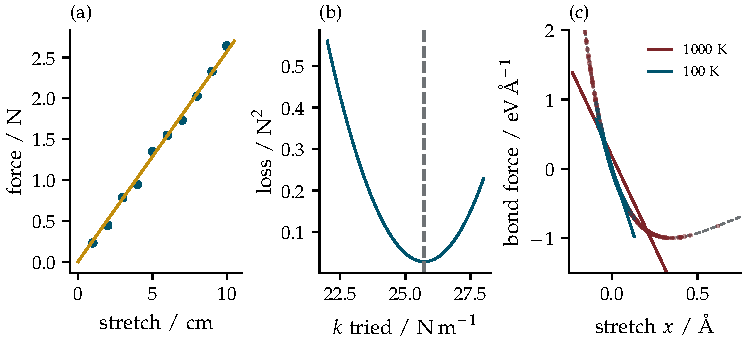
\includegraphics{ch18_learning/bond}
\caption{One weight learned by least squares. (a) A spring's force read
on a dial with an error of \SI{0.05}{\newton} at ten stretches (readings
drawn by computer for \SI{25}{\newton\per\metre}), and the line through
the origin of least squares. (b) The sum of squared misses against the
stiffness tried; the fit is its lowest point (dashed). (c) The A--B
molecule of Chapter~16 under Langevin dynamics: the force along the bond
against its stretch, every \SI{50}{\femto\second} of \SI{20}{\pico
\second}, at 100 and \SI{1000}{\kelvin}, with the Morse force (grey
dashed) and the straight lines of least squares.}
\label{fig:lo-bond}
\end{figure}

\begin{keyidea}
Learning a model from data is the lowering of a loss, here the sum of
squared misses. For a model linear in its weights the least loss solves
the normal equations $X^{\mathsf T}X\boldsymbol{\theta} = X^{\mathsf T}\vb{y}$ at
once. A fit answers the question its data pose: a line through the forces
of a hot run gives the stiffness averaged over the stretches that run
explores.
\end{keyidea}

\notebook{18}{fit a spring and a bond, and change the temperature of the
bond's run}

\begin{selfcheck}
Ten readings of a spring's force at stretches $x_i$ all lie exactly on a
line through the origin. What is $\mathcal{L}(\hat k)$, and what does the formula
for the error of $\hat k$ then give?
\end{selfcheck}

%=============================================================================!
% 18.2  BASIS FUNCTIONS AND OVERFITTING                                       !
%=============================================================================!
\section{Basis functions and overfitting}
\label{sec:lo-basis}

A curve drawn freehand through a dozen noisy points can be made to pass
through every one of them, if it is allowed to wiggle; between the
points it then swings far from any sensible value, and a new point
measured in a gap lands nowhere near it. The curve has learned the
noise. A smoother curve that passes near the points, rather than
through them, predicts the gaps better. Choosing how freely a model may
bend is the first decision of any fit.

\subsection*{A curve through noisy readings}

The readings here are argon's pair energy $\varphi(r)$ between
\SI{3.3}{\angstrom} and $2\sigma = \SI{6.8}{\angstrom}$, where the switched
potential of Chapter~12 is the plain Lennard-Jones energy, read at 15
distances drawn at random with an error of \SI{0.2}{\milli\electronvolt}
added, as a first-principles calculation adds its own small errors
(\cref{fig:lo-basis}a). The model is a polynomial,
\begin{equation*}
   \hat\varphi(r) = \sum_{j=0}^{p-1}w_js^j , \qquad
   s = \frac{r - \SI{5.05}{\angstrom}}{\SI{1.75}{\angstrom}} ,
\end{equation*}
in the scaled distance $s$, which runs from $-1$ to 1 over the range; the
functions $s^j$ are its \emph{basis functions}, and the columns of the
design matrix are their values at the readings. The scaling matters for
the arithmetic, not for the fit: the powers of $r$ itself range from 1
to $6.8^{14} \approx \num{5e11}$, and \cref{sec:lo-descent} measures what
that does. The weights come from the normal equations
(\cref{eq:lo-normal}), and the fit is judged on 200 distances spread
evenly over the range, without noise, which the fit never saw: the
\emph{test}.

\Cref{fig:lo-basis}(b) tells the story. As the degree of the polynomial
rises from 0, the rms miss on the 15 training readings falls, from
\num{3.38} to \SI{0.20}{\milli\electronvolt} at degree 8, near the
noise, and then further, to zero at degree 14, where 15 weights pass a
curve through 15 readings exactly. The miss on the test falls with it at
first, to \SI{0.28}{\milli\electronvolt} at degree 8, and then rises
steeply: \SI{3.9}{\milli\electronvolt} at degree 9, 140 at 12 and
\SI{41}{\electronvolt} at 14, where the curve swings between the readings
(\cref{fig:lo-basis}a). A model with too few weights misses the curve,
\emph{underfitting}; one with too many learns the noise of its readings
as if it were part of the curve, \emph{overfitting}, and the training
miss falling below the noise of the readings is its sign. Only data the
model has not seen can tell the two apart, since the training miss
improves with every weight added.

The functions themselves can carry knowledge. The Lennard-Jones energy is
a sum of $(\sigma/r)^{12}$ and $(\sigma/r)^6$, and a model built on those
two functions has two weights to find. Fitted to the same 15 readings,
they come out as \num{0.04051} and \SI{-0.04073}{\electronvolt}, against
$4\varepsilon = \SI{0.04136}{\electronvolt}$ and $-4\varepsilon$, and
the test miss is \SI{0.090}{\milli\electronvolt}, a third of the best
polynomial's with two weights against nine. A learned potential faces
the same choice on a larger scale: a model that knows the forces between
atoms depend only on their distances and on the elements needs far fewer
readings than one that must discover it, which is what planned Chapter~20 builds
into the description of an atom's surroundings.

\begin{figure}[htb]
\centering
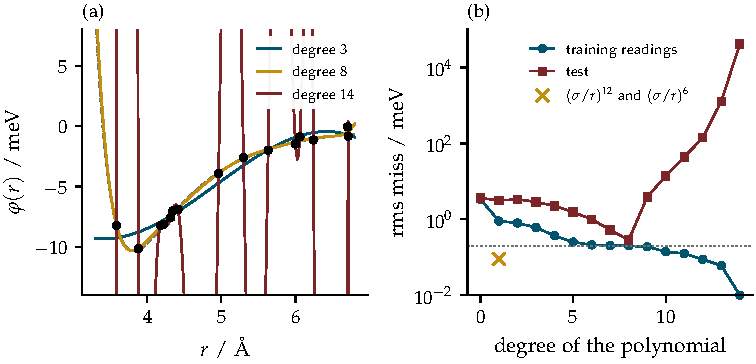
\includegraphics{ch18_learning/basis}
\caption{Basis functions and overfitting. (a) Argon's pair energy (grey
dashed) read at 15 distances with an error of
\SI{0.2}{\milli\electronvolt} (dots), and the polynomials of degree 3, 8
and 14 in the scaled distance fitted to the readings by least squares.
(b) The rms miss on the training readings and on a test of 200
noise-free distances against the degree, with the noise (dotted) and the
test miss of the two functions $(\sigma/r)^{12}$ and $(\sigma/r)^6$
(cross). At degree 14 the curve passes through every reading, and its
training miss, zero, is drawn on the axis.}
\label{fig:lo-basis}
\end{figure}

\begin{keyidea}
A model linear in its weights is a sum of basis functions, and the
number of them sets how freely it bends. Too few underfit; too many
learn the noise, which shows as a training miss below the noise of the
readings and a test miss that grows. Only readings the model has not
seen judge it. Functions that carry the physics need fewer weights and
fewer readings.
\end{keyidea}

\notebook{18}{change the degree of the polynomial and watch the training
and test misses part}

\begin{selfcheck}
A polynomial of degree 14 is fitted to 15 readings. Why is its training
miss zero whatever the readings, and what does that say about the
training miss as a measure of a model?
\end{selfcheck}

%=============================================================================!
% 18.3  RIDGE REGULARISATION AND ITS BAYESIAN READING                         !
%=============================================================================!
\section{Ridge regularisation and its Bayesian reading}
\label{sec:lo-ridge}

A tailor cutting a suit from a few measurements prefers a pattern close
to a standard one, and departs from it only as far as the measurements
demand; a stray reading of the sleeve does not make the jacket
lopsided. A fit can be given the same preference. The polynomial of
degree 14 in \cref{fig:lo-basis} passed through every reading with
weights as large as \num{1e4}\,\si{\electronvolt}, which cancel one
another to near zero at the readings and nowhere else. A penalty on large
weights keeps the curve from paying that price for each stray reading.

\subsection*{The penalised loss}

\emph{Ridge regularisation} adds to the sum of squared misses the
squared length of the weight vector, times a number $\lambda \ge 0$:
\begin{equation}
   L(\vb{w}) = \lvert X\vb{w} - \vb{y}\rvert^2 + \lambda\lvert\vb{w}\rvert^2 .
   \label{eq:lo-ridge}
\end{equation}
Its gradient is that of the toolbox of \cref{sec:lo-loss} plus the
gradient of $\lambda\sum_jw_j^2$, which is $2\lambda\vb{w}$, so the least
loss solves
\begin{align*}
   2X^{\mathsf T}(X\vb{w} - \vb{y}) + 2\lambda\vb{w} &= \vb{0}
      && \text{setting the gradient to zero}\\
   \bigl(X^{\mathsf T}X + \lambda I\bigr)\vb{w} &= X^{\mathsf T}\vb{y}
      && \text{dividing by 2 and gathering the terms in $\vb{w}$,}
\end{align*}
with $I$ the identity matrix. The penalty is a sum of squares too: it is
the squared miss of the extra equations $\sqrt\lambda\,w_j = 0$, one for
each weight, so the ridge loss is the ordinary loss of the design matrix
$X$ with $\sqrt\lambda\,I$ stacked below it, against $\vb{y}$ with $p$
zeros below it, which is how \texttt{mdlab.learn.least\_squares} solves it:

\begin{code}
def least_squares(X: ArrayLike, y: ArrayLike, ridge: float = 0.0) -> NDArray:
    X = np.asarray(X, dtype=float)
    y = np.asarray(y, dtype=float)
    if ridge:
        p = X.shape[1]
        X = np.vstack([X, np.sqrt(ridge) * np.eye(p)])
        y = np.concatenate([y, np.zeros((p, *y.shape[1:]))])
    return np.linalg.lstsq(X, y, rcond=None)[0]
\end{code}

\noindent NumPy's \texttt{lstsq} finds the least squared miss without
forming $X^{\mathsf T}X$, whose entries are squares and so lose half the
digits that a badly scaled $X$ still holds.

Why the penalty helps shows in the eigenvectors of $X^{\mathsf T}X$, a
symmetric matrix with eigenvalues $d_k \ge 0$ and orthonormal eigenvectors
$\vb{v}_k$ (\cref{sec:os-modes}). Writing the weights as $\vb{w} =
\sum_kc_k\vb{v}_k$ and taking the dot product of the normal equations with
$\vb{v}_k$,
\begin{equation*}
   (d_k + \lambda)\,c_k = \vb{v}_k\cdot X^{\mathsf T}\vb{y} , \qquad
   c_k = \frac{\vb{v}_k\cdot X^{\mathsf T}\vb{y}}{d_k + \lambda} ,
\end{equation*}
since $X^{\mathsf T}X\vb{v}_k = d_k\vb{v}_k$ and the other eigenvectors
are perpendicular to $\vb{v}_k$. Without the penalty each component is
divided by $d_k$. A direction with a small $d_k$ is one the readings
barely constrain, a combination of basis functions that is nearly zero at
every reading, and dividing by a small $d_k$ turns the noise of the
readings into a large weight along it. The penalty leaves directions with
$d_k \gg \lambda$ almost as they were and shrinks those with $d_k \ll
\lambda$ towards zero by the factor $d_k/(d_k + \lambda)$.

\subsection*{Choosing the penalty}

$\lambda$ is not learned from the training readings, which always prefer
$\lambda = 0$. Fifteen more readings, drawn as the first were, are held
back for \emph{validation}, and $\lambda$ is chosen to make the miss on
them least. For the polynomial of degree 14 (\cref{fig:lo-ridge}a), the
validation miss is least at $\lambda = 10^{-3}$, where the test miss is
\SI{0.15}{\milli\electronvolt}, half that of the best polynomial without
the penalty and close to the two-function fit's 0.09; the weights shrink
from a length of \SI{1.1e4}{\electronvolt} to \SI{0.014}{\electronvolt}
(\cref{fig:lo-ridge}b). Below $\lambda \approx 10^{-6}$ the noise is
learned again; above $10^{-2}$ the curve is held too stiff to follow the
well. The test, a third set, is kept for the end: having chosen
$\lambda$ by the validation readings, their miss is no longer an honest
estimate of the miss on new ones.

\begin{figure}[htb]
\centering
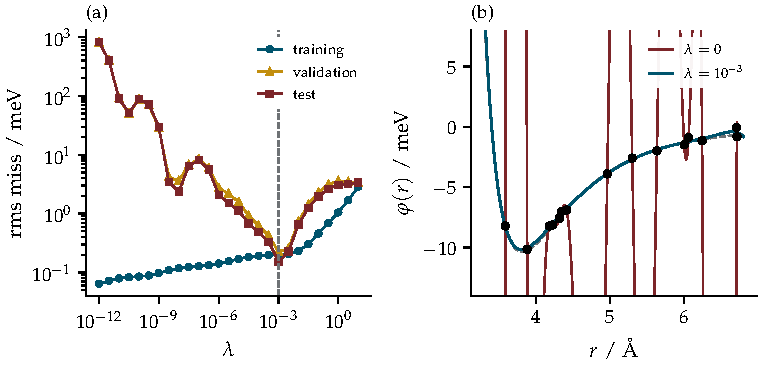
\includegraphics{ch18_learning/ridge}
\caption{Ridge regularisation of the polynomial of degree 14. (a) The
rms miss on the 15 training readings, on 15 validation readings and on
the noise-free test against $\lambda$, with the $\lambda$ of least
validation miss (dashed). (b) The fit without the penalty and with
$\lambda = 10^{-3}$, against the pair energy (grey dashed) and the
training readings.}
\label{fig:lo-ridge}
\end{figure}

\begin{toolbox}[Conditional probability and Bayes's rule]
Of $N$ equally likely outcomes, $N_A$ have a property $A$, $N_B$ a
property $B$ and $N_{AB}$ both. The probability of $B$ among the
outcomes with $A$, the \emph{conditional probability} of $B$ given $A$,
is $\mathcal{P}(B\mid A) = N_{AB}/N_A$, and multiplying and dividing by
$N$,
\begin{equation*}
   \mathcal{P}(B\mid A) = \frac{N_{AB}/N}{N_A/N}
   = \frac{\mathcal{P}(A\text{ and }B)}{\mathcal{P}(A)} .
\end{equation*}
The same holds with $A$ and $B$ exchanged, so $\mathcal{P}(A\text{ and
}B) = \mathcal{P}(B\mid A)\,\mathcal{P}(A) = \mathcal{P}(A\mid
B)\,\mathcal{P}(B)$, and dividing by $\mathcal{P}(B)$ gives
\emph{Bayes's rule},
\begin{equation*}
   \mathcal{P}(A\mid B) = \frac{\mathcal{P}(B\mid A)\,\mathcal{P}(A)}
   {\mathcal{P}(B)} .
\end{equation*}
For quantities with densities (\cref{sec:sm-probability}) the same rule
holds with densities in place of probabilities. Read with $A$ a cause and
$B$ an observation, it turns the chance of the observation given each
cause into the chance of each cause given the observation.
\end{toolbox}

\subsection*{The Bayesian reading}

The penalty has a second meaning. Suppose the readings are the model's
predictions plus independent Gaussian noise of spread $\sigma$, so that
the density of the readings given the weights is
\begin{equation*}
   p(\vb{y}\mid\vb{w}) \propto \prod_i\exp\Bigl[-\frac{(y_i -
   [X\vb{w}]_i)^2}{2\sigma^2}\Bigr]
   = \exp\Bigl[-\frac{\lvert X\vb{w} - \vb{y}\rvert^2}{2\sigma^2}\Bigr] ,
\end{equation*}
a product of Gaussians (\cref{sec:sm-maxwell}), and suppose that before
any reading each weight was believed to lie near zero, within a spread
$\sigma_w$: a \emph{prior} density $p(\vb{w}) \propto
\exp(-\lvert\vb{w}\rvert^2/2\sigma_w^2)$. Bayes's rule gives the density
of the weights given the readings, the \emph{posterior},
\begin{equation*}
   p(\vb{w}\mid\vb{y}) = \frac{p(\vb{y}\mid\vb{w})\,p(\vb{w})}{p(\vb{y})}
   \propto \exp\Bigl[-\frac{\lvert X\vb{w} - \vb{y}\rvert^2}{2\sigma^2}
   - \frac{\lvert\vb{w}\rvert^2}{2\sigma_w^2}\Bigr] ,
\end{equation*}
where $p(\vb{y})$ does not depend on $\vb{w}$. The most probable weights
make the bracket least; multiplying it by $-2\sigma^2$, they make
$\lvert X\vb{w} - \vb{y}\rvert^2 + (\sigma^2/\sigma_w^2)\lvert
\vb{w}\rvert^2$ least, the ridge loss with
\begin{equation*}
   \lambda = \frac{\sigma^2}{\sigma_w^2} .
\end{equation*}
Ridge regression is the most probable fit under Gaussian noise and a
Gaussian belief that the weights are small. The chosen $\lambda = 10^{-3}$
with the noise of \SI{0.2}{\milli\electronvolt} corresponds to $\sigma_w
= \sigma/\sqrt\lambda = \SI{6.3}{\milli\electronvolt}$, a belief that
each weight is of the size of the well's depth, which is sensible for a
curve whose values are of that size and whose basis functions lie
between $-1$ and 1. The posterior is more than its most probable point:
it gives every weight a spread, and through them the curve an error bar,
which the next section obtains in another way.

\begin{keyidea}
Ridge regularisation adds $\lambda\lvert\vb{w}\rvert^2$ to the loss, so
the least loss solves $(X^{\mathsf T}X + \lambda I)\vb{w} = X^{\mathsf
T}\vb{y}$; it shrinks the directions the readings barely constrain.
$\lambda$ is chosen on validation readings and the result judged on test
readings never used for any choice. It is the most probable fit under
Gaussian noise of spread $\sigma$ and a Gaussian prior of spread
$\sigma_w$ on the weights, with $\lambda = \sigma^2/\sigma_w^2$.
\end{keyidea}

\notebook{18}{vary the penalty and see which directions of the weights
shrink}

\begin{selfcheck}
The readings' noise doubles while the prior belief about the weights is
unchanged. What happens to $\lambda$, and to how closely the fit follows
the readings?
\end{selfcheck}

%=============================================================================!
% 18.4  KERNELS AND GAUSSIAN PROCESSES                                        !
%=============================================================================!
\section{Kernels and Gaussian processes}
\label{sec:lo-gp}

A forecaster who knows the temperature at a few weather stations
estimates it in a village between them by leaning on the nearest
stations most, since temperatures a few kilometres apart are alike, and
says how sure they are: close to a station they are nearly certain, far
from every station they can say little more than what is usual for the
season. A Gaussian process makes this reasoning exact. It needs no basis
functions chosen in advance, only a statement of how alike the values at
two points are expected to be, and it returns, at every point, an
estimate and an error bar.

\subsection*{A random function}

Before any reading, the unknown curve $f(x)$ is treated as random: its
values at any set of points are jointly Gaussian with mean zero, and the
values at two points $x$ and $x'$ have the covariance
\begin{equation}
   k(x, x') = h^2\exp\Bigl[-\frac{(x - x')^2}{2\ell^2}\Bigr] ,
   \label{eq:lo-kernel}
\end{equation}
the \emph{kernel}. Each value has the variance $k(x, x) = h^2$, a spread
$h$ about zero; values at points much closer than the length scale $\ell$
are nearly equal, their covariance almost $h^2$, and values much further
apart are nearly independent. The kernel is the forecaster's belief that
nearby temperatures are alike, written as a number. Readings $y_i =
f(x_i) + \epsilon_i$ with independent noise $\epsilon_i$ of spread
$\sigma$ then have the covariances $K_{ij} = k(x_i, x_j) +
\sigma^2\delta_{ij}$, the noise adding to each reading's own variance
only. The value $f(x_\ast)$ at a new point and the readings are jointly
Gaussian, with the covariances $k(x_\ast, x_i)$, collected in the vector
$\vb{k}_\ast$. The question is what the readings say about $f(x_\ast)$:
the Gaussian conditioned on them.

\begin{toolbox}[A Gaussian conditioned on another]
Let $a$ and $b$ be jointly Gaussian with mean zero, variances
$\sigma_a^2$ and $\sigma_b^2$ and covariance $c = \ens{ab}$. The number
$e = a - (c/\sigma_b^2)\,b$ has the covariance with $b$
\begin{equation*}
   \ens{eb} = \ens{ab} - \frac{c}{\sigma_b^2}\ens{b^2}
   = c - \frac{c}{\sigma_b^2}\sigma_b^2 = 0 .
\end{equation*}
A linear combination of jointly Gaussian numbers is Gaussian, and two
jointly Gaussian numbers with zero covariance are independent, since
their joint density, $\exp(-e^2/2\sigma_e^2 - b^2/2\sigma_b^2)$ up to a
constant, is the product of the two densities (\cref{sec:sm-probability}).
So knowing $b$ says nothing about $e$, and $a = (c/\sigma_b^2)b + e$ has,
given $b$, the mean $(c/\sigma_b^2)\,b$ and the variance of $e$,
\begin{align*}
   \sigma_e^2 &= \ens{a^2} - 2\frac{c}{\sigma_b^2}\ens{ab}
      + \frac{c^2}{\sigma_b^4}\ens{b^2}
      && \text{expanding the square of $e$}\\
   &= \sigma_a^2 - \frac{2c^2}{\sigma_b^2} + \frac{c^2}{\sigma_b^2}
   = \sigma_a^2 - \frac{c^2}{\sigma_b^2}
      && \text{collecting the terms in $c^2$.}
\end{align*}
The same steps with $b$ a vector of readings, of covariance matrix
$K$, and $\vb{c} = \ens{a\vb{b}}$ a vector, give the mean $\vb{c}^{\mathsf
T}K^{-1}\vb{b}$ and the variance $\sigma_a^2 - \vb{c}^{\mathsf
T}K^{-1}\vb{c}$, the division by $\sigma_b^2$ becoming the inverse matrix
(\cref{sec:ro-remove}). Knowing $b$ moves the mean and always lowers
the variance.
\end{toolbox}

\noindent With $a = f(x_\ast)$, $\vb{b} = \vb{y}$ and $\vb{c} =
\vb{k}_\ast$, the readings give $f(x_\ast)$ the mean and variance
\begin{equation}
   \bar f(x_\ast) = \vb{k}_\ast^{\mathsf T}K^{-1}\vb{y} , \qquad
   \operatorname{var} f(x_\ast) = h^2 - \vb{k}_\ast^{\mathsf T}K^{-1}
   \vb{k}_\ast .
   \label{eq:lo-gp}
\end{equation}
The mean is a weighted sum of the readings, as the forecaster's estimate
is, the weights $K^{-1}\vb{k}_\ast$ larger for readings near $x_\ast$.
Close to a reading the variance falls to about the noise's $\sigma^2$;
far from all of them $\vb{k}_\ast$ vanishes and the variance returns to
the prior's $h^2$. This is the posterior of the weights of
\cref{sec:lo-ridge} in another form: a Gaussian process is ridge
regression on as many basis functions as the kernel implies, possibly
infinitely many, solved through the $n\times n$ matrix $K$ of the
readings rather than the $p\times p$ matrix $X^{\mathsf T}X$ of the
weights\cite{Rasmussen2006}. \texttt{mdlab.learn.GaussianProcess} solves
it with the factor $K = LL^{\mathsf T}$, $L$ lower triangular, by which a
system with $K$ becomes two systems with triangles, each solved one
unknown at a time.

\subsection*{The pair energy from eight readings}

Eight readings of argon's pair energy, drawn as in \cref{sec:lo-basis},
are fitted with $h = \SI{10}{\milli\electronvolt}$, about the depth of the
well, and the known noise of \SI{0.2}{\milli\electronvolt}
(\cref{fig:lo-gp}). The length scale still has to be chosen, and the
readings themselves choose it through their \emph{marginal likelihood},
the density of the readings under the prior. Since $\vb{y}$ is Gaussian
with covariance $K$, its logarithm is
\begin{equation*}
   \ln p(\vb{y}) = -\tfrac12\vb{y}^{\mathsf T}K^{-1}\vb{y}
   - \tfrac12\ln\det K - \tfrac n2\ln2\pi ,
\end{equation*}
the multivariable form of the Gaussian of \cref{sec:sm-maxwell}. The
first term rewards a prior under which the readings are typical; the
second penalises a prior so loose, with $\ell$ so short, that it would
have found any readings typical. Their balance peaks at $\ell =
\SI{0.70}{\angstrom}$ (\cref{fig:lo-gp}c). There the mean follows the
readings, and its standard deviation is at most
\SI{0.2}{\milli\electronvolt} at the readings and
\SI{1.1}{\milli\electronvolt} midway across the widest gap, from 3.36 to
\SI{4.13}{\angstrom}. A length a quarter as long makes the curve sag
towards zero between readings, with an honest but useless band; one four
times as long makes it too stiff, with a band too narrow
(\cref{fig:lo-gp}b).

The band must also be right. Over the test, \num{0.75} of the noise-free
values lie within twice the standard deviation at $\ell =
\SI{0.70}{\angstrom}$, against the 0.95 that a correct Gaussian band
holds, and the misses gather at the steep wall below \SI{3.8}{\angstrom}
and at the bottom of the well, where no reading falls. A kernel with one
length scale cannot be both smooth enough for the slow tail and supple
enough for the wall, and the error bar is only as good as the kernel's
belief. At a quarter of the length the band holds 0.99 of the test, and
at four times only 0.15. Gaussian processes on atoms, with kernels built
on descriptions of each atom's surroundings, are the Gaussian
Approximation Potentials\cite{Bartok2010}, among the first learned
potentials; their error bar is what lets a learned potential say where
it needs another first-principles calculation, the subject of
planned Chapter~23.

\begin{figure}[htb]
\centering
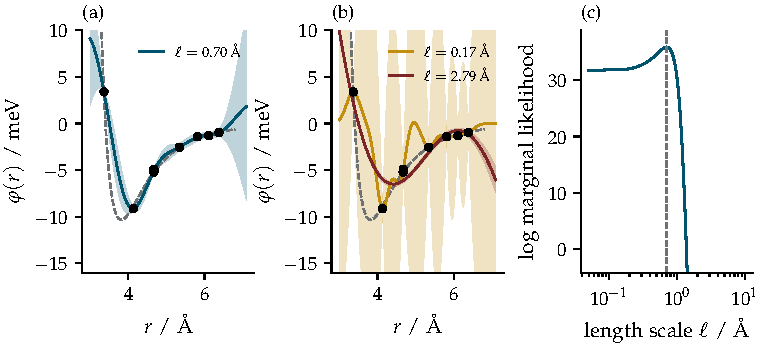
\includegraphics{ch18_learning/gp}
\caption{A Gaussian process through eight readings of argon's pair
energy (dots, noise \SI{0.2}{\milli\electronvolt}), with $h =
\SI{10}{\milli\electronvolt}$, against the pair energy (grey dashed). (a)
The posterior mean and twice its standard deviation (band) for the length
scale of greatest marginal likelihood. (b) The same for a length a
quarter of that and four times it. (c) The log marginal likelihood of the
readings against the length scale, with its greatest value (dashed).}
\label{fig:lo-gp}
\end{figure}

\begin{keyidea}
A Gaussian process treats the unknown curve as a random function whose
values covary by a kernel; conditioning on the readings gives the mean
$\vb{k}_\ast^{\mathsf T}K^{-1}\vb{y}$ and the variance $h^2 -
\vb{k}_\ast^{\mathsf T}K^{-1}\vb{k}_\ast$ at every point, an estimate with
an error bar that grows away from the readings. The marginal likelihood
chooses the kernel's length. The error bar is only as reliable as the
kernel, and checking it against held-out values is part of the fit.
\end{keyidea}

\notebook{18}{move the readings and the length scale and watch the band}

\begin{selfcheck}
A Gaussian process is conditioned on one reading $y_1$ at $x_1$, with no
noise. What are its mean and variance at $x_1$, and at a point very far
from $x_1$?
\end{selfcheck}

%=============================================================================!
% 18.5  GRADIENT DESCENT                                                      !
%=============================================================================!
\section{Gradient descent}
\label{sec:lo-descent}

A walker caught in fog on a hillside, wanting the valley floor, feels the
slope under their feet and steps downhill, then feels again. Short steps
are safe but slow; a long step on a steep slope can carry the walker
across a narrow valley and up the far side, higher than they started,
and a run of such steps climbs out of the valley altogether. The normal
equations solved the fits so far in one calculation, but most models,
the networks of planned Chapter~19 among them, have losses that no formula
minimises, and they are walked down instead.

\subsection*{The step and its limit}

\emph{Gradient descent} repeats the step
\begin{equation}
   \vb{w} \leftarrow \vb{w} - \eta\,\grad L(\vb{w}) ,
   \label{eq:lo-descent}
\end{equation}
moving the weights against the gradient, the direction in which the loss
falls fastest (\cref{sec:en-gradient}), by an amount set by the
\emph{learning rate} $\eta$. Near a minimum with positive curvature in
every direction, a smooth loss is approximated to second order by a
quadratic bowl, just as a potential energy is near a stable minimum
(\cref{sec:os-modes}). In this approximation, with $\vb{e} = \vb{w} - \vb{w}^\ast$ the
departure from the minimum $\vb{w}^\ast$ and $A$ the matrix of second
derivatives there, the Hessian,
\begin{equation*}
   L = L^\ast + \tfrac12\vb{e}^{\mathsf T}A\vb{e} , \qquad
   \grad L = A\vb{e} .
\end{equation*}
For this quadratic, a step changes the departure by
\begin{align*}
   \vb{e} &\leftarrow \vb{e} - \eta A\vb{e} = (I - \eta A)\,\vb{e}
      && \text{subtracting $\vb{w}^\ast$ from both sides of the step}\\
   c_k &\leftarrow (1 - \eta\lambda_k)\,c_k
      && \text{along each eigenvector of $A$, of eigenvalue $\lambda_k$,}
\end{align*}
the components $c_k$ of $\vb{e}$ along the eigenvectors changing
independently, as the normal modes of a vibrating molecule do. Each
shrinks only if $\lvert1 - \eta\lambda_k\rvert < 1$, that is $0 < \eta <
2/\lambda_k$, and the steepest direction, with the largest eigenvalue
$\lambda_{\max}$, sets the limit:
\begin{equation}
   \eta < \frac{2}{\lambda_{\max}} .
   \label{eq:lo-limit}
\end{equation}
This is the stability limit of an integrator in another guise
(\cref{sec:in-stability}): the fastest vibration of a molecule bounds the
time step, and the steepest direction of a loss bounds the learning rate.
Between $1/\lambda_{\max}$ and $2/\lambda_{\max}$ the factor $1 -
\eta\lambda_{\max}$ is negative, and the steep component flips sign at
every step while it shrinks, the zig-zag of the walker across the valley.

\Cref{fig:lo-descent} walks a loss of two weights whose Hessian has the
eigenvalues 1 and 10, so $2/\lambda_{\max} = 0.2$. At $\eta = 0.05$ the
factors are 0.95 and 0.50, and the shallow direction crawls; at 0.18 they
are 0.82 and $-0.80$, and the path zig-zags down the valley; at 0.205
the steep factor is $-1.05$, and the path climbs out. The best fixed rate
makes the slowest factor as small as it can be, which it is when the
two extreme factors are equal and opposite, $1 - \eta\lambda_{\min} =
-(1 - \eta\lambda_{\max})$:
\begin{equation*}
   \eta = \frac{2}{\lambda_{\min} + \lambda_{\max}} , \qquad
   1 - \eta\lambda_{\min} = \frac{\lambda_{\max} - \lambda_{\min}}
   {\lambda_{\max} + \lambda_{\min}} = \frac{\kappa - 1}{\kappa + 1} ,
\end{equation*}
with $\kappa = \lambda_{\max}/\lambda_{\min}$ the \emph{condition number}
of the Hessian. Here $\eta = 0.182$, the factor is 0.818, and since the
loss falls as the square of the factor, it falls a millionfold in
$\ln10^6/(-2\ln0.818) = 34$ steps.

\subsection*{The condition number decides}

For a large condition number the factor is $1 - 2/(\kappa + 1)$, and the
steps for a millionfold fall grow in proportion to $\kappa$, about
$\kappa\ln10^6/4$. The least-squares loss has the Hessian $2X^{\mathsf
T}X$, and the polynomial fits of \cref{sec:lo-basis} are badly
conditioned: $X^{\mathsf T}X$ has $\kappa = 74$ for degree 3 in the scaled
distance, \num{4.6e6} for degree 8 and \num{5.1e16} for degree 14, and
for degree 8 in $r$ itself \num{3.3e26}, beyond what the 16 digits of
double precision can even resolve. Gradient descent at its best fixed rate
would need about 260 steps for degree 3 and \num{1.6e7} for degree 8.
Scaling the variable, as \cref{sec:lo-basis} did, is the first remedy;
the solvers of the normal equations are another; and the optimisers of
\cref{sec:lo-momentum} are a third, for the losses that have no normal
equations.

A loss is \emph{convex} if the straight line between any two points of
its graph lies on or above the graph; a quadratic with a Hessian whose
eigenvalues are all positive or zero is convex, and the least-squares
loss, with Hessian $2X^{\mathsf T}X$, is one. A convex loss has no local
minima besides its least value, so gradient descent at a stable rate
reaches it from any start. The losses of neural networks are not convex,
and where gradient descent ends then depends on where it began
(planned Chapter~19).

\begin{figure}[htb]
\centering
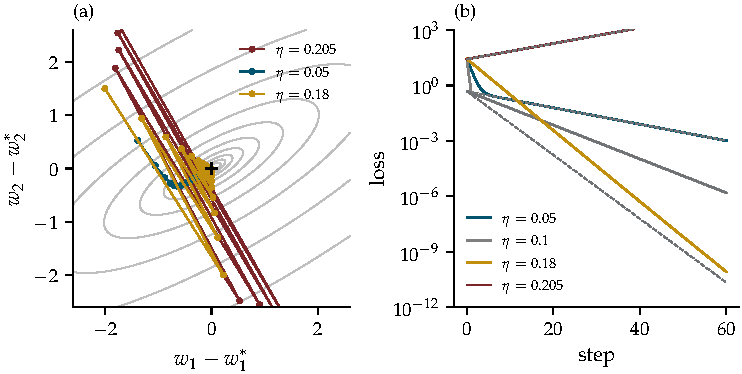
\includegraphics{ch18_learning/descent}
\caption{Gradient descent on a quadratic loss of two weights whose
Hessian has the eigenvalues 1 and 10 along axes turned by \ang{30}. (a)
The paths at learning rates of 0.05, 0.18 and 0.205 over the contours of
the loss (first 25 steps, 9 for the rate that diverges). (b) The loss
against the step for rates of 0.05, 0.1, 0.18 and 0.205, with the term of
each rate's slowest direction, $\frac12\lambda c^2(1 - \eta\lambda)^{2t}$
for $c$ the start's component along it (dashed).}
\label{fig:lo-descent}
\end{figure}

\begin{keyidea}
Gradient descent steps against the gradient by the learning rate $\eta$.
Near the minimum each eigen-direction of the Hessian shrinks by $1 -
\eta\lambda$ a step, so $\eta < 2/\lambda_{\max}$, the stability limit of
an integrator again; at the best fixed rate the slowest direction
shrinks by $(\kappa - 1)/(\kappa + 1)$, and the condition number $\kappa$
sets how many steps are needed. A convex loss has one least value, which
descent at a stable rate reaches.
\end{keyidea}

\notebook{18}{walk down a valley at different rates and condition numbers}

\begin{selfcheck}
A loss has a Hessian with eigenvalues 0.5 and 50. What is the largest
stable learning rate, and what factor does the slow direction shrink by
at the best fixed rate?
\end{selfcheck}

%=============================================================================!
% 18.6  STOCHASTIC GRADIENTS                                                  !
%=============================================================================!
\section{Stochastic gradients}
\label{sec:lo-sgd}

A poll does not ask every voter; a thousand chosen at random give the
share of a party to within a few per cent, at a tiny fraction of the
cost. The gradient of a loss is an average over the readings, and it too
can be estimated from a few of them. A learned potential is trained on
hundreds of thousands of configurations, each with hundreds of forces,
and an exact gradient over all of them for every step would make training
impossibly slow.

\subsection*{A gradient from a few readings}

Written as the mean over $n$ readings of a loss $\ell_i$ for each,
$L = \frac1n\sum_i\ell_i(\vb{w})$, the loss has the gradient $\grad L =
\frac1n\sum_i\grad\ell_i$, a mean of $n$ numbers. A \emph{mini-batch} of
$b$ readings chosen at random gives the estimate $\vb{g} =
\frac1b\sum_{i\in\text{batch}}\grad\ell_i$, whose average over the
possible batches is the true gradient. If the readings' gradients scatter
about their mean with the spread $\sigma_g$, each component of $\vb{g}$
scatters by
\begin{equation*}
   \frac{\sigma_g}{\sqrt b} ,
\end{equation*}
the error of a mean of $b$ independent samples (\cref{sec:cv-mean}).
\emph{Stochastic gradient descent} steps with $\vb{g}$ in place of
$\grad L$, one step per batch, and a pass through all the readings, an
\emph{epoch}, takes $n/b$ steps for the cost of one exact gradient.

\Cref{fig:lo-sgd} fits the force of the A--B bond at \SI{300}{\kelvin},
2001 readings from \cref{sec:lo-loss}, with a straight line in the
scaled stretch $x/\sigma_x$, its loss the mean squared miss. At the least
loss, where the exact gradient is zero, the gradient of the slope's
weight from batches of ten readings scatters by \num{0.180}, against the
$\sigma_g/\sqrt{10} = \num{0.185}$ that the readings' own spread gives
(\cref{fig:lo-sgd}b); its histogram is not yet Gaussian, since a mean of
ten skewed numbers is still skewed, but its width is as predicted.

\subsection*{A noise floor, and a rate that falls}

The noise has a cost. With the rate fixed at half the stability limit,
full-batch descent reaches the least loss in under ten epochs, while
batches of ten never settle: after 50 epochs their loss is still
\num{4.7e-3}\,(\si{\electronvolt\per\angstrom})$^2$ above the least, with
spikes far above it (\cref{fig:lo-sgd}a). Near the minimum the true
gradient vanishes but the estimate does not, and each step moves the
weights by about $\eta\sigma_g/\sqrt b$ in a random direction, so the
weights wander in a cloud whose size is set by the rate. A rate that
falls as training proceeds, here $\eta/(1 + \text{epoch}/5)$, shrinks the
cloud, and after 50 epochs the loss lies \num{4.4e-4} above the least.
The rate must fall slowly enough that the steps still add up to the
distance the weights must travel, and fast enough that the wandering
dies away; schedules of this kind, and the batch size, are among the
settings that every training run of planned Chapter~19 and after reports.

Each run of the figure evaluated the gradient of one reading
\num{100050} times; the full-batch run took 50 steps with them, the
mini-batch runs \num{10050}. When the readings are many and alike, as
the frames of a long run are, a mini-batch gradient is nearly as good as
the full one at a small fraction of the cost, and taking many cheap
noisy steps is faster than taking a few exact ones.

\begin{figure}[htb]
\centering
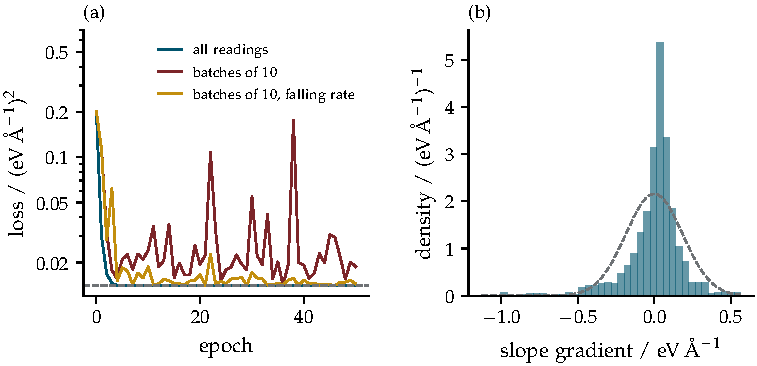
\includegraphics{ch18_learning/sgd}
\caption{Gradients from mini-batches. The force of the A--B bond at
\SI{300}{\kelvin} (2001 readings) fitted by a straight line in the
scaled stretch. (a) The mean squared miss over all the readings against
the epoch, for gradient descent on all of them, for batches of ten at a
fixed rate, and for batches of ten at a rate that falls, with the least
loss (dashed). (b) The gradient of the slope's weight from 1000 batches
of ten at the least loss, against a Gaussian of spread $\sigma_g/\sqrt{10}$
(dashed).}
\label{fig:lo-sgd}
\end{figure}

\begin{keyidea}
A mini-batch of $b$ readings estimates the gradient with an error that
falls as $\sigma_g/\sqrt b$, at $b/n$ of the cost. At a fixed rate the
weights end in a cloud about the minimum whose size the rate sets; a
rate that falls slowly shrinks it.
\end{keyidea}

\notebook{18}{change the batch size and the schedule and watch the loss
settle}

\begin{selfcheck}
Batches of 10 give a gradient that scatters by 0.18. What batch size
would bring the scatter to 0.06, and how many steps would an epoch of
2001 readings then take?
\end{selfcheck}

%=============================================================================!
% 18.7  MOMENTUM AND ADAM                                                     !
%=============================================================================!
\section{Momentum and Adam}
\label{sec:lo-momentum}

A heavy block sliding down a long, gently tilted gutter with steep sides
gathers speed along the gutter, since every push points the same way
there, while across it the pushes alternate from one wall to the other
and friction damps the swaying. The walker of \cref{sec:lo-descent} has
no memory: each step depends only on the slope underfoot, so along a
long shallow valley it creeps, and across a steep one it zig-zags. Giving
the steps memory, as the block's speed is a memory of past pushes, cures
much of both.

\subsection*{Momentum}

\emph{Gradient descent with momentum} keeps a velocity $\vb{v}$, a
running sum of past gradients that decays by a factor $\mu < 1$ a step,
and moves the weights along it:
\begin{equation}
   \vb{v} \leftarrow \mu\vb{v} + \grad L(\vb{w}) , \qquad
   \vb{w} \leftarrow \vb{w} - \eta\vb{v} .
   \label{eq:lo-momentum}
\end{equation}
The block is more than a picture. Writing $\vb{w}_t$ for the weights after
$t$ steps, the second rule gives $\eta\vb{v}_t = \vb{w}_{t-1} - \vb{w}_t$
at every step. Multiplying the first rule by $-\eta$ and substituting
gives
\begin{equation*}
   \vb{w}_{t+1} - \vb{w}_t = \mu(\vb{w}_t - \vb{w}_{t-1})
   - \eta\grad L(\vb{w}_t) ,
\end{equation*}
and moving $\vb{w}_t - \vb{w}_{t-1}$ to the left,
\begin{equation*}
   (\vb{w}_{t+1} - 2\vb{w}_t + \vb{w}_{t-1})
   + (1 - \mu)(\vb{w}_t - \vb{w}_{t-1}) = -\eta\grad L(\vb{w}_t) .
\end{equation*}
The first bracket is a second difference, the change of the step from
one step to the next, an acceleration, and the second a velocity: this is
Newton's law with friction, $m\ddot{\vb{w}} + \gamma\dot{\vb{w}} =
-\grad L$ (\cref{sec:os-damped}), discretised with a step of one, the
mass one, the friction $1 - \mu$ and the force $\eta$ times the gradient.
Momentum turns the descent into the damped motion of a particle on the
loss.

On a quadratic loss each eigen-direction of the Hessian again moves on
its own, the component $c_t$ along an eigenvector of eigenvalue
$\lambda$ following $c_{t+1} = (1 + \mu - \eta\lambda)\,c_t - \mu
c_{t-1}$, the line above with $\grad L$ replaced by $\lambda c_t$.
Trying $c_t = z^t$, as for the oscillations of \cref{sec:in-stability},
\begin{equation*}
   z^2 - (1 + \mu - \eta\lambda)\,z + \mu = 0 .
\end{equation*}
The product of the two roots is $\mu$, so when they are complex, a pair
of conjugates of equal size, both have $\lvert z\rvert = \sqrt\mu$: the
component swings and shrinks by $\sqrt\mu$ a step, whatever $\lambda$.
They are complex while $(1 + \mu - \eta\lambda)^2 \le 4\mu$, and the
best choice, due to Polyak\cite{Polyak1964}, puts both ends of the range
of eigenvalues on the edge of this condition, $1 + \mu -
\eta\lambda_{\min} = 2\sqrt\mu$ and $1 + \mu - \eta\lambda_{\max} =
-2\sqrt\mu$:
\begin{align*}
   (1 - \sqrt\mu)^2 &= \eta\lambda_{\min} , \quad
   (1 + \sqrt\mu)^2 = \eta\lambda_{\max}
      && \text{as squares}\\
   \frac{1 + \sqrt\mu}{1 - \sqrt\mu} &= \sqrt\kappa
      && \text{dividing, and the root}\\
   \sqrt\mu &= \frac{\sqrt\kappa - 1}{\sqrt\kappa + 1}
      && \text{solving for $\sqrt\mu$,}
\end{align*}
the first line writing $1 + \mu \mp 2\sqrt\mu$ as $(1 \mp \sqrt\mu)^2$.
Adding the square roots of the first line's two equations gives $2 =
\sqrt\eta\,(\sqrt{\lambda_{\min}} + \sqrt{\lambda_{\max}})$, so $\eta =
4/(\sqrt{\lambda_{\max}} + \sqrt{\lambda_{\min}})^2$.
The asymptotic contraction factor in every direction is $(\sqrt\kappa - 1)/(\sqrt\kappa + 1)$ a step,
against $(\kappa - 1)/(\kappa + 1)$ without momentum, and the steps
needed grow as $\sqrt\kappa$ instead of $\kappa$. For the valley of
\cref{fig:lo-optimisers}, with eigenvalues 1 and 100, the factors are
0.818 and 0.980: momentum brings the loss below $10^{-8}$ in 77 steps,
while gradient descent at its best fixed rate has not in 300. The steep
weight shows the difference (\cref{fig:lo-optimisers}a): without
momentum it flips sign at every step and barely shrinks, by the factor
$-0.98$; with momentum it rings and dies away, the damped swing of
Chapter~4.

\subsection*{Adam}

The networks of the later chapters are trained with
Adam\cite{Kingma2014}, which gives each weight a step of its own size.
It keeps two running means of each weight's gradient, of the gradient
and of its square,
\begin{equation*}
   m \leftarrow \beta_1m + (1 - \beta_1)\,g , \qquad
   s \leftarrow \beta_2s + (1 - \beta_2)\,g^2 ,
\end{equation*}
with $\beta_1 = 0.9$ and $\beta_2 = 0.999$ by default, each a mean over
roughly the last $1/(1 - \beta)$ steps, 10 and 1000, weighted towards the
recent ones. Both start at zero, which biases them low at first: with a
steady gradient $g$, after $t$ steps
\begin{equation*}
   m_t = (1 - \beta_1)\sum_{k=0}^{t-1}\beta_1^kg
   = (1 - \beta_1)\frac{1 - \beta_1^t}{1 - \beta_1}\,g
   = (1 - \beta_1^t)\,g ,
\end{equation*}
by the sum of a geometric series, so dividing by $1 - \beta_1^t$ undoes
the bias, and likewise for $s$. The step is
\begin{equation*}
   w \leftarrow w - \eta\,\frac{\hat m}{\sqrt{\hat s} + \epsilon} , \qquad
   \hat m = \frac{m}{1 - \beta_1^t} , \quad \hat s = \frac{s}{1 - \beta_2^t} ,
\end{equation*}
with $\epsilon = 10^{-8}$ guarding against a division by zero. For a
steady gradient $\hat m/\sqrt{\hat s}$ is $\pm1$, so each weight moves by
about $\eta$ a step whatever the size of its gradient; multiplying one
weight's gradients by a constant multiplies $\hat m$ and $\sqrt{\hat s}$
alike and leaves its steps unchanged. In \texttt{mdlab}:

\begin{code}
class Adam:
    def __init__(self, rate: float = 1e-3, beta1: float = 0.9,
                 beta2: float = 0.999, eps: float = 1e-8):
        self.rate, self.beta1, self.beta2, self.eps = rate, beta1, beta2, eps
        self.m = self.s = None
        self.t = 0

    def step(self, w: NDArray, g: NDArray) -> NDArray:
        if self.m is None:
            self.m, self.s = np.zeros_like(g), np.zeros_like(g)
        self.t += 1
        self.m = self.beta1 * self.m + (1 - self.beta1) * g
        self.s = self.beta2 * self.s + (1 - self.beta2) * g * g
        m_hat = self.m / (1 - self.beta1**self.t)
        s_hat = self.s / (1 - self.beta2**self.t)
        return w - self.rate * m_hat / (np.sqrt(s_hat) + self.eps)
\end{code}

\noindent A test checks that its steps, and those of \texttt{Momentum},
match PyTorch's \texttt{Adam} and \texttt{SGD} with momentum on a loss of
two weights to the last digit.

The scaling is Adam's strength and its limit. A valley whose steep and
shallow directions lie along the weights, as when one weight multiplies
a feature a hundred times larger than another's, is a valley of badly
scaled weights, and Adam evens them out: with the rate 0.05 it reaches
$10^{-8}$ in 189 steps (\cref{fig:lo-optimisers}b). The same valley
turned by \ang{45}, its steep direction a mixture of both weights, gives
each weight a similar gradient, Adam's scaling has nothing to even out,
and after 300 steps its loss is still 0.49, worse than plain descent's
\num{0.0014}, while momentum still needs only 85
(\cref{fig:lo-optimisers}c). Adam is robust where the scales of the
weights differ widely and are not known in advance, as in a network,
which is why it is the common default; a narrow valley at an angle it
leaves as it found it.

\begin{figure}[htb]
\centering
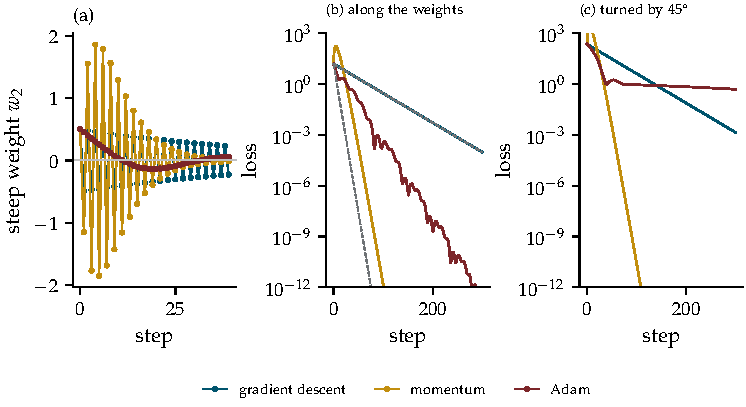
\includegraphics{ch18_learning/optimisers}
\caption{Gradient descent, momentum and Adam in a valley whose Hessian
has the eigenvalues 1 and 100, from $(-2.5, 0.5)$: descent at its best
fixed rate $2/(\lambda_{\min} + \lambda_{\max})$, momentum with Polyak's
rate and $\mu$, Adam with the rate 0.05. (a) The steep weight against
the step, the valley's axes along the weights. (b) The loss against the
step there, with the factors per step that theory gives descent and
momentum (dashed). (c) The loss in the same valley turned by \ang{45}.}
\label{fig:lo-optimisers}
\end{figure}

\begin{keyidea}
Momentum adds to the step a decaying memory of past gradients; it is
damped motion on the loss, and on a quadratic with Polyak's choice it
has the asymptotic contraction factor $(\sqrt\kappa - 1)/(\sqrt\kappa + 1)$ a step.
Adam divides each weight's running mean gradient by the root of its
running mean square, with both corrected for their start at zero, so that
every weight moves at about the rate whatever the scale of its gradient;
it evens out badly scaled weights, and leaves a narrow valley at an angle
as narrow as it was.
\end{keyidea}

\notebook{18}{race the three optimisers down a valley, and turn the valley}

\begin{selfcheck}
For a Hessian with $\kappa = 10^4$, by what factor does the slow direction
shrink in a step of gradient descent at its best fixed rate, and of
momentum with Polyak's choice?
\end{selfcheck}

%=============================================================================!
% 18.8  TRAINING, VALIDATION AND TEST                                         !
%=============================================================================!
\section{Training, validation and test}
\label{sec:lo-splits}

A student who revises from past papers and then sits an exam made of the
same questions scores well without having learned the subject; the
score measures memory alone. A fitted model is judged the
same way, on readings it has not seen, and the judgement is only as
honest as the separation of those readings from the ones it learned
from. With the frames of a molecular dynamics run that separation is
subtler than it looks.

\subsection*{Three sets}

The readings are divided before any fitting. The \emph{training} set
fixes the weights; the \emph{validation} set chooses everything that the
training set cannot, such as the degree of a polynomial, the penalty
$\lambda$, the learning rate or the moment to stop
(\cref{sec:lo-ridge}); the \emph{test} set is opened once, at the end, to
report how well the chosen model predicts. Every choice made by looking
at a set spends some of that set's honesty, which is why the test is
touched last.

The division assumes that the sets are independent samples of the
readings the model will meet. Frames of a run are not: a frame
\SI{10}{\femto\second} after another holds nearly the same positions and
nearly the same energy, and \cref{sec:cv-correlation} measured how long
such a memory lasts, as the statistical inefficiency $g$, the number of
consecutive samples worth one independent one.

\subsection*{Frames that leak}

Two runs of Chapter~12's liquid argon were made with every
\SI{10}{\femto\second} step kept, as first-principles runs often are, and
a model was asked to learn each frame's potential energy $U$ from the
histogram of its \num{32640} pair distances in 110 bins of
\SI{0.05}{\angstrom}. The task is well posed: $U$ is the sum of the pair
energy over the pairs, so it is linear in the histogram, through the pair
energy at each bin, with a miss from the binning alone of
\SI{22.5}{\milli\electronvolt} against a spread of $U$ of
\SI{175}{\milli\electronvolt}. Ridge regression ($\lambda = 10^{-2}$, the
110 counts scaled by the training frames' mean and spread) learned $U$
from the first frames of one run, with a fifth held out for validation,
and was tested on frames of the other run, every \SI{50}{\femto\second},
a run it never saw (\cref{fig:lo-leak}).

At \SI{10}{\femto\second} the energy has $g = 109$ frames, so a training
run of \SI{2}{\pico\second}, 200 frames, holds about two independent
ones. Held out at random, its validation frames each have training
frames \SI{10}{\femto\second} either side of them, nearly identical, and
the validation miss is $(30.5 \pm 4.4)$\,\si{\milli\electronvolt} over ten
random splits, while the independent run gives $(128 \pm
16)$\,\si{\milli\electronvolt}, four times more: the random split measures
how well the model recalls its neighbours. Held out in whole blocks of
\SI{0.5}{\pico\second}, the validation miss is $(92 \pm
22)$\,\si{\milli\electronvolt}, close to the truth. With \SI{4}{\pico
\second} the random split still reports 21.7 against 37.8, the blocked
one 34.8; only at 10 and \SI{20}{\pico\second}, about 9 and 18 independent
frames, do all three agree near the binning's own floor, since a model
with enough independent frames no longer needs the neighbours.

The cure is to split by time, into whole blocks longer than the memory
$g$, or better whole runs, for validation and test. The same care
applies to every quantity computed from the training set alone, such as
the mean and spread that scale the features, which must not be computed
with the validation frames in. A learned potential's reported error
means little without the split that produced it.

\begin{figure}[htb]
\centering
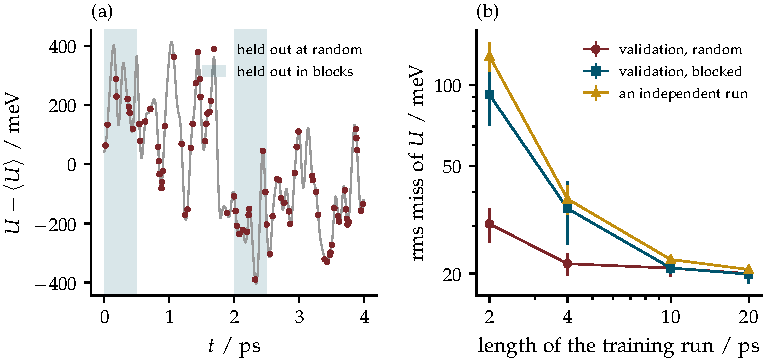
\includegraphics{ch18_learning/leak}
\caption{Consecutive frames leak between splits. Liquid argon, a frame
every \SI{10}{\femto\second}; ridge regression learns each frame's
potential energy from the histogram of its pair distances. (a) The
energy over \SI{4}{\pico\second}, with the frames that a random split
holds out (dots) and those that a split into blocks of
\SI{0.5}{\pico\second} holds out (shaded). (b) The rms miss of $U$ on
validation frames held out at random and in blocks, and on an
independent run, against the length of the training run, with the
spread over ten splits.}
\label{fig:lo-leak}
\end{figure}

\begin{keyidea}
Training readings fix the weights, validation readings choose the
settings, and test readings, touched once, report the result. All three
must be independent samples; consecutive frames of a run are not, and
split at random they let a model look up its neighbours, reporting a miss
four times too small here. Split by blocks longer than the statistical
inefficiency, or by whole runs.
\end{keyidea}

\notebook{18}{split a run's frames at random and in blocks and compare the
misses}

\begin{selfcheck}
A first-principles run of \SI{10}{\pico\second} keeps every
\SI{1}{\femto\second} step, and its energy has $g = 400$ steps. About how
many independent frames does it hold, and how long should each validation
block be?
\end{selfcheck}

%=============================================================================!
% 18.9  WHAT THE TRAINING LOOKS LIKE                                          !
%=============================================================================!
\section{What the training looks like}
\label{sec:lo-training}

A run of molecular dynamics is read through its energies, and a training
run through its losses. The curve of the loss against the step, for the
training readings and for the validation readings, is the first thing to
look at when a model is trained, and most faults show in it.
\Cref{fig:lo-training} trains the polynomials of \cref{sec:lo-basis} on
the fifteen readings of argon's pair energy by lowering the mean squared
miss from zero weights, once healthily and then broken in four ways, and
\cref{tab:lo-faults} gathers the checks.

\textit{Healthy.} Degree 8 in the scaled distance, Adam at the rate
$10^{-4}$, 40\,000 steps: the training miss falls to
\SI{0.202}{\milli\electronvolt} and the validation miss with it, to
0.187, both at the noise of \SI{0.2}{\milli\electronvolt}
(\cref{fig:lo-training}a). Two curves that fall together and level at the
noise are the picture of a model that has learned what the readings
hold.

\textit{The rate.} Gradient descent on the same fit at 0.9 of its
stability limit $2/\lambda_{\max}$ brings the training miss to
\SI{0.28}{\milli\electronvolt} in 400 steps; at 1.1 of it the miss grows
without bound, to \SI{1.7e32}{\milli\electronvolt}; at a thousandth of
it the miss has fallen only to \SI{3.6}{\milli\electronvolt}
(\cref{fig:lo-training}b). A loss that rises, or swings with growing
amplitude, means a rate past the limit; one that barely moves, a rate far
below it. Adam shows a milder form of the first: at a fixed rate of
$10^{-3}$ its training miss jumps by up to
\SI{0.24}{\milli\electronvolt} in a single step late in training, when
its running mean square has decayed and the steps no longer shrink with
the gradient, against \SI{0.005}{\milli\electronvolt} at $10^{-4}$, the
smaller rate removing the spikes.

\textit{Overfitting.} Degree 14 with no penalty, Adam at $10^{-4}$ for
\num{e5} steps: the training miss keeps falling, to
\SI{0.150}{\milli\electronvolt}, below the noise, while the validation
miss is least, \SI{0.38}{\milli\electronvolt}, after 160 steps and then
rises to \SI{2.95}{\milli\electronvolt} (\cref{fig:lo-training}c). Two
curves that part, the training miss below the noise and the validation
miss climbing, mean the model is learning the noise. Stopping at the
step of least validation miss, \emph{early stopping}, keeps the model of
that step and works as a penalty does, since the weights have not yet
grown into the directions the readings barely constrain; a penalty or
fewer weights cure it outright.

\textit{Unscaled features.} Degree 8 in $r$ itself, whose design has the
condition number \num{3.3e26} against \num{4.6e6} for the scaled
distance, trained by gradient descent at 0.9 of each one's stability
limit: after 2000 steps the training miss is
\SI{5.3}{\milli\electronvolt} with powers of $r$ and
\SI{0.22}{\milli\electronvolt} with the scaled distance
(\cref{fig:lo-training}d). A loss that falls a little and then crawls,
with no sign of the noise floor, points to badly scaled inputs before it
points to a bad model; scaling each input to a spread of about one is the
cure, and the reason the readings of a learned potential are normalised
before training.

\textit{A leaked split.} The fault that the loss curves cannot show is
the one of \cref{sec:lo-splits}: with frames split at random, training
and validation misses fall together to a healthy-looking floor, 30.5
against an independent run's \SI{128}{\milli\electronvolt}. Only a
validation set separated in time, or a separate run, reveals it.

\begin{figure}[htb]
\centering
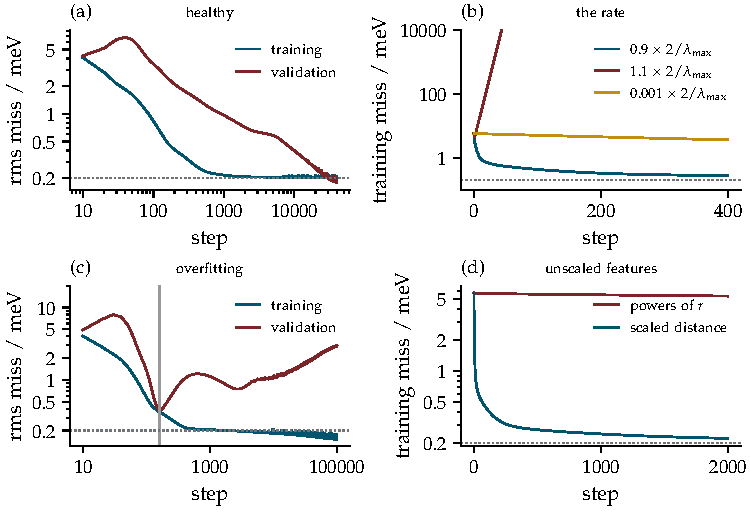
\includegraphics{ch18_learning/training}
\caption{What the training looks like: the rms miss on the fifteen
training readings of argon's pair energy, and on fifteen validation
readings, against the step, from zero weights. (a) Healthy: degree 8,
Adam at $10^{-4}$. (b) Gradient descent at 0.9 and 1.1 of its stability
limit and at a thousandth of it. (c) Overfitting: degree 14, Adam at
$10^{-4}$, with the step of least validation miss (grey). (d) Degree 8 in
$r$ itself and in the scaled distance, gradient descent at 0.9 of each
one's limit. The noise of the readings, \SI{0.2}{\milli\electronvolt},
dotted.}
\label{fig:lo-training}
\end{figure}

\begin{table}[htb]
\centering
\small
\caption{Faults of training, the check that catches each, and its value
in the healthy run and in the broken one.}
\label{tab:lo-faults}
\begin{tabular}{@{}>{\raggedright\arraybackslash}p{0.22\linewidth}
   >{\raggedright\arraybackslash}p{0.34\linewidth}
   >{\raggedright\arraybackslash}p{0.17\linewidth}
   >{\raggedright\arraybackslash}p{0.17\linewidth}@{}}
\toprule
fault & check & healthy & broken\\
\midrule
rate past the limit & training miss after 400 steps & \SI{0.28}{\milli
\electronvolt} & \SI{1.7e32}{\milli\electronvolt}\\
rate far too small & training miss after 400 steps & \SI{0.28}{\milli
\electronvolt} & \SI{3.6}{\milli\electronvolt}\\
Adam's rate too large & largest jump of the training miss in a step &
\SI{0.005}{\milli\electronvolt} & \SI{0.24}{\milli\electronvolt}\\
overfitting & validation miss at the end against its least &
\num{0.19} against 0.18 (degree 8) & \num{2.95} against \SI{0.38}{\milli
\electronvolt}\\
unscaled features & condition number of $X^{\mathsf T}X$ & \num{4.6e6} &
\num{3.3e26}\\
leaked split & validation miss against an independent run's &
\num{92} against 128 (blocked) & \num{30.5} against
\SI{128}{\milli\electronvolt}\\
\bottomrule
\end{tabular}
\end{table}

\begin{keyidea}
The training and validation losses against the step are read as a run's
energies are: falling together to the noise is healthy; a rising or
swinging loss means a rate past the limit; a crawl, a rate too small or
inputs badly scaled; curves that part, overfitting, cured by early
stopping, a penalty or fewer weights. A leaked split looks healthy, and
only a validation set separated in time reveals it.
\end{keyidea}

\notebook{18}{break a training run in each of these ways and read its
loss curves}

\begin{selfcheck}
A model's training loss falls steadily, and its validation loss falls
for a while and then rises. What is happening, and which step's weights
should be kept?
\end{selfcheck}

%=============================================================================!
% 18.S  WHAT WE NOW HAVE                                                      !
%=============================================================================!
\unnumbered{What we now have}

Learning a model from readings is the lowering of a loss. For a model
linear in its weights, a sum of basis functions, the sum of squared
misses is least where the normal equations $X^{\mathsf T}X\vb{w} =
X^{\mathsf T}\vb{y}$ hold, and a fit answers the question its readings
pose: a line through the forces of a hot run gives the bond's stiffness
averaged over the stretches it explores.
More basis functions bend the
model more freely and, beyond a point, learn the noise, which only
readings the model has not seen reveal. A ridge penalty
$\lambda\lvert\vb{w}\rvert^2$ shrinks the directions the readings barely
constrain, is the most probable fit under Gaussian noise and a Gaussian
prior with $\lambda = \sigma^2/\sigma_w^2$, and is chosen on validation
readings. A Gaussian process conditions a random function on the
readings and returns an estimate with an error bar, whose kernel the
marginal likelihood chooses and whose band must still be checked.

Gradient descent walks a loss down with a rate bounded by $2/\lambda_{\max}$,
the stability limit of an integrator again, at a pace set by the
condition number; mini-batches estimate the gradient with an error
$\sigma_g/\sqrt b$ at a fraction of the cost; momentum is damped motion
on the loss and, on a quadratic with the optimal settings, has asymptotic
contraction factor $(\sqrt\kappa - 1)/(\sqrt\kappa
+ 1)$ a step; Adam evens out badly scaled weights.
Training, validation
and test readings must be independent, and consecutive frames of a run
are not. In this chapter's example, a random split makes the validation
error four times too small; separating the time intervals gives a much
closer estimate of the error on an independent run. The training and validation curves
show the remaining faults of a training run.

Planned Chapter~19 builds models that are not linear in their weights, neural
networks, computes their gradients by the chain rule run backwards, and
trains them on energies and forces with these optimisers.

%=============================================================================!
% 18.A  ANSWERS TO THE CHECKS                                                 !
%=============================================================================!
\unnumbered{Answers to the checks}
\label{sec:lo-answers}

\answerto{sec:lo-loss}Zero, since the line passes through every reading.
The misses about the fitted line are then all zero, so the estimated
$\sigma_{\mathrm m}$ and the error of $\hat k$ are zero too: ten perfect
readings leave no trace of their noise, and an error estimated from the
misses is only as good as the misses are typical.

\answerto{sec:lo-basis}Fifteen weights and fifteen readings make the
design matrix square, and for distinct distances it can be inverted, so
$X\vb{w} = \vb{y}$ has an exact solution, which makes the loss zero. Any
fifteen readings, noise and all, are fitted exactly, so a training miss
can always be driven to zero and says nothing about prediction.

\answerto{sec:lo-ridge}$\lambda = \sigma^2/\sigma_w^2$ grows four times,
so the penalty weighs more against the misses, and the fit follows the
readings less closely, keeping nearer the smooth curve that the prior
prefers: noisier readings deserve less trust.

\answerto{sec:lo-gp}At $x_1$, $K = h^2$ and $\vb{k}_\ast = h^2$, so the
mean is $h^2y_1/h^2 = y_1$ and the variance $h^2 - h^4/h^2 = 0$: the curve
passes through the reading with no doubt. Far from $x_1$, $\vb{k}_\ast$
vanishes, the mean returns to the prior's zero and the variance to $h^2$.

\answerto{sec:lo-descent}The rate must lie below $2/\lambda_{\max} = 2/50 = 0.04$. With $\kappa =
100$ the slow direction shrinks by $(100 - 1)/(100 + 1) = 0.980$ a step.

\answerto{sec:lo-sgd}The scatter falls as $1/\sqrt b$, so a third of it
needs nine times the batch, 90 readings; an epoch of 2001 readings is then
$2001/90 = 22.2$, so 23 steps, the last batch short.

\answerto{sec:lo-momentum}With $\sqrt\kappa = 100$, gradient descent
shrinks by $(10^4 - 1)/(10^4 + 1) = 0.9998$ and momentum by $(100 -
1)/(100 + 1) = 0.980$ a step: about 100 times fewer steps for the same
fall.

\answerto{sec:lo-splits}\num{10000} steps worth one independent frame
each 400 are about 25 independent frames. A validation block should be
longer than the memory, several times 400 steps, say 1 to
\SI{2}{\pico\second}, or better a separate run.

\answerto{sec:lo-training}The model is learning the noise of its
training readings, overfitting. Keep the weights of the step where the
validation loss was least, early stopping, or retrain with a penalty or
fewer weights.

%=============================================================================!
% 18.E  EXERCISES                                                             !
%=============================================================================!
\unnumbered{Exercises}
\label{sec:lo-exercises}

The exercises run from questions of understanding, through calculations,
to short derivations marked `show that'. Full solutions are in
\hyperref[sec:lo-solutions]{`Solutions to the exercises'} at the end of
the book, and Notebook~18 checks every numerical answer.

\begin{exercise}[the least loss]
\label{ex:lo-least}
For the line through the origin, show that the least loss is
$L(\hat k) = \sum_iF_i^2 - \bigl(\sum_ix_iF_i\bigr)^2/\sum_ix_i^2$.
\end{exercise}

\begin{exercise}[the error of a stiffness]
\label{ex:lo-error}
A spring is stretched by 1, 2, \dots, \SI{10}{\centi\metre} and its force
read with an error of \SI{0.05}{\newton} each, independently. What is
the error of the fitted stiffness?
\end{exercise}

\begin{exercise}[a line with an intercept]
\label{ex:lo-intercept}
For the model $\hat y = c + sx$, write $X^{\mathsf T}X$ and $X^{\mathsf
T}\vb{y}$ in terms of sums over the readings, and show that the normal
equations give the slope $s = \sum_i(x_i - \bar x)(y_i - \bar y)/\sum_i(x_i
- \bar x)^2$ of \cref{sec:cv-drift}.
\end{exercise}

\begin{exercise}[a stiffness that changes]
\label{ex:lo-stiffness}
Show that the stiffness of the Morse well, $-\dd F/\dd x$ for the force
$F = -\dd U_{\mathrm M}/\dd x$, is $2Da^2(2\mathrm{e}^{-2ax} -
\mathrm{e}^{-ax})$, and that it is $2Da^2(1 - 3ax)$ to first order in
$x$. By what fraction does it change over $x = \pm\SI{0.0345}{\angstrom}$
for $a = \SI{2}{\per\angstrom}$?
\end{exercise}

\begin{exercise}[as many weights as readings]
\label{ex:lo-square}
Show that if the design matrix $X$ is square and has an inverse, the
normal equations give $X\vb{w} = \vb{y}$ exactly, so the fit passes
through every reading.
\end{exercise}

\begin{exercise}[shrinkage]
\label{ex:lo-shrink}
With $X^{\mathsf T}X$ having the eigenvalues $d_k$, show that each
component of the ridge weights along an eigenvector is that of the
weights without the penalty times $d_k/(d_k + \lambda)$, for $d_k > 0$.
\end{exercise}

\begin{exercise}[the prior's spread]
\label{ex:lo-prior}
With readings of noise $\sigma = \SI{0.2}{\milli\electronvolt}$, what
spread $\sigma_w$ of the weights does $\lambda = 10^{-3}$ express, and
what $\lambda$ would express $\sigma_w = \SI{1}{\milli\electronvolt}$?
\end{exercise}

\begin{exercise}[conditioning two Gaussians]
\label{ex:lo-condition}
Two jointly Gaussian numbers $a$ and $b$ have mean zero, variances 4 and
1, and covariance 1.5. Given $b = 2$, what are the mean and the variance
of $a$?
\end{exercise}

\begin{exercise}[a process with one reading]
\label{ex:lo-one}
A Gaussian process with the kernel of \cref{eq:lo-kernel} is conditioned
on one reading $y_1$ at $x_1$ with noise of spread $\sigma$. Show that
its mean at $x$ is $y_1\,\mathrm{e}^{-(x - x_1)^2/2\ell^2}\,h^2/(h^2 +
\sigma^2)$, and find its variance.
\end{exercise}

\begin{exercise}[a learning rate]
\label{ex:lo-rate}
A loss has a Hessian with the eigenvalues 2 and 200. Find the upper
bound on a stable rate, the best fixed rate, the factor by which the slow direction
shrinks at it, and the steps that bring the loss down a millionfold.
\end{exercise}

\begin{exercise}[steps against the condition number]
\label{ex:lo-kappa}
Show that for a large condition number the best fixed rate needs about
$\kappa\ln(1/\varepsilon)/4$ steps to bring the loss down by the factor
$\varepsilon$, using $\ln(1 + y) \approx y$ for small $y$.
\end{exercise}

\begin{exercise}[the batch for a precision]
\label{ex:lo-batch}
The readings' gradients scatter by $\sigma_g = 0.585$. What batch gives
the mini-batch gradient a scatter of 0.05?
\end{exercise}

\begin{exercise}[the memory of momentum]
\label{ex:lo-memory}
With $\mu = 0.9$ and no gradient, after how many steps has the velocity
fallen to $1/\mathrm{e}$ of its value, and what is the friction $1 - \mu$
of the equivalent damped motion?
\end{exercise}

\begin{exercise}[Polyak's momentum]
\label{ex:lo-polyak}
For eigenvalues 1 and 100, find Polyak's $\sqrt\mu$, $\mu$ and $\eta$, and
use the asymptotic contraction factors to estimate the steps needed to
shrink the slow direction by $10^{-4}$, with momentum and with gradient
descent at its best fixed rate. Ignore the initial transient.
\end{exercise}

\begin{exercise}[Adam's correction]
\label{ex:lo-adam}
A weight's gradient is a steady $g$. With $\beta_1 = 0.9$ and $\beta_2 =
0.999$, what are $m$ and $s$ after 10 steps, and by what factor would the
step be too large if neither were corrected for its start at zero?
\end{exercise}

\begin{exercise}[Adam and scale]
\label{ex:lo-scale}
Show that, with $\epsilon$ neglected, Adam's step for a weight is
unchanged when all that weight's gradients are multiplied by a constant
$c > 0$.
\end{exercise}

\begin{exercise}[independent frames]
\label{ex:lo-frames}
A run's energy, kept every \SI{10}{\femto\second}, has the statistical
inefficiency $g = 109$. How many independent frames are there in 2 and
in \SI{20}{\pico\second}?
\end{exercise}

\begin{exercise}[why a neighbour helps]
\label{ex:lo-neighbour}
A validation frame of a random split has training frames
\SI{10}{\femto\second} before and after it. Explain why a model that interpolates nearby frames can
predict this frame well while performing poorly on a new run.
\end{exercise}

\begin{exercise}[a plan for the splits]
\label{ex:lo-plan}
Fifty first-principles runs of lithium in graphite, each
\SI{5}{\pico\second} at one of ten temperatures, are to train a learned
potential. Propose training, validation and test sets, and say what each
must not share.
\end{exercise}



% Appendix E is drafted in appendices/ and awaits its software version table.
% Appendices A to E join as they are built; until then F keeps its letter.
\appendix
\setcounter{chapter}{5}
%=============================================================================!
% APPENDIX F  A GALLERY OF FAULTS                                             !
% Every fault met in the sections 'What the trajectory looks like' of        !
% Chapters 11 to 17, with its symptom, check and cure.                        !
%=============================================================================!
\chapter{A gallery of faults}
\label{app:gallery}

Chapters~11--17 end by breaking their own runs on purpose
and finding the check that catches each fault. This appendix gathers them
in one table, in the order of the chapters, each with what it looks like,
the check that finds it (a function of \texttt{mdlab.diagnostics} where
there is one), and the cure. \texttt{diagnostics.health\_report} runs the
checks of continuity, the centre of mass, overlaps, energy, temperature
and velocities on a run of \texttt{mdlab} or, through
\texttt{io.read\_run}, of any code that ASE can read
(\cref{sec:ip-trajectory}), and Notebook~F passes the cached runs of
Chapters~11, 12, 13 and~16, healthy and broken, through it.

\begingroup
\small
\begin{longtable}{@{}>{\raggedright\arraybackslash}p{0.20\linewidth}
   >{\raggedright\arraybackslash}p{0.26\linewidth}
   >{\raggedright\arraybackslash}p{0.22\linewidth}
   >{\raggedright\arraybackslash}p{0.22\linewidth}@{}}
\caption{Faults of molecular dynamics runs, their symptoms, the checks
that find them and their cures.}
\label{tab:app-gallery}\\
\toprule
fault & what it looks like & check & cure\\
\midrule
\endfirsthead
\toprule
fault & what it looks like & check & cure\\
\midrule
\endhead
\bottomrule
\endfoot
\multicolumn{4}{@{}l}{\textit{Integrating and constraining
(\cref{sec:cs-trajectory})}}\\
step too long & the total energy fluctuates widely, not falling as
$\dt^2$ & \texttt{energy\_\allowbreak fluctuation} & a shorter step, or held bonds\\
jumping cutoff & spikes of the total energy as pairs cross the cutoff &
\texttt{energy\_\allowbreak fluctuation} & the Ewald sum for charges
(\cref{sec:md-ewald}), or a potential switched off smoothly
(\cref{sec:pe-cutoffs})\\
wrong units & a kinetic energy per freedom far from $\frac12\kB T$ & $K$ at
the start & velocities converted between units\\
wrapped wrongly & held distances wrong by a cell & \texttt{bond\_error} &
the nearest image in the constraints\\
overlap & an enormous force at the start & \texttt{largest\_\allowbreak force},
\texttt{closest\_\allowbreak approach} & the start relaxed or rebuilt\\
loose constraints & the total energy drifts & \texttt{energy\_\allowbreak drift} & a
tighter tolerance\\
drift kept & the centre of mass travels & \texttt{centre\_\allowbreak of\_\allowbreak mass\_\allowbreak path} &
the total momentum removed\\
resonance & the energy drifts under multiple time steps &
\texttt{energy\_\allowbreak drift} & a shorter outer step\\
\multicolumn{4}{@{}l}{\textit{Ensembles (\cref{sec:sm-trajectory})}}\\
freedoms miscounted & the temperature is wrong by a ratio of counts & $T$
against the value asked & $3N - n_{\mathrm c} - 3$ freedoms\\
lattice start & the temperature halves as energy flows into the potential &
mean $T$ against $T(0)$ & a start drawn at twice the temperature, half
of which flows into the potential (\cref{sec:sm-equipartition}), or an
equilibrated one\\
drift counted & a temperature that includes the flight of the whole &
total momentum & the momentum removed\\
masses ignored & species start at different temperatures & $T$ of each
species & velocities drawn for each mass\\
not Gaussian & velocities spread evenly, not as Maxwell-Boltzmann &
\texttt{excess\_\allowbreak kurtosis} & velocities drawn from the Gaussian\\
no sharing & energy stays in the modes it started in & the energy of each
mode & a longer run, or a thermostat acting on each atom\\
\multicolumn{4}{@{}l}{\textit{Thermostats (\cref{sec:th-trajectory})}}\\
coupling too strong & a temperature spread far below canonical & spread of
$T$ against $\sqrt{2/N_{\mathrm f}}\,T$ & CSVR or a chain, or weaker
coupling\\
coupling too weak & runs that have not reached the temperature & mean $T$
of several runs & longer equilibration, or stronger coupling while it
lasts\\
flying ice cube & kinetic energy collecting in the centre of mass & growth
of its kinetic energy & a thermostat that samples the canonical ensemble\\
one atom, one variable & a density that is not canonical & the density
of $U$ against the exact one & a chain, or Langevin\\
wrong $N_{\mathrm f}$ & a temperature on the wrong count of freedoms & $T$
over the true freedoms & the code's count checked\\
centre as diffusion & $D$ too large & $D$ with the centre removed & the
centre of mass removed\\
\multicolumn{4}{@{}l}{\textit{Pressure (\cref{sec:pr-trajectory})}}\\
virial from wrapped positions & a pressure that moves with the origin & $P$
after moving the origin & the virial from pair separations\\
kinetic part dropped & a pressure read too low by $N\kB T/V$; under a
barostat, a volume too small & $P$ with $2K$ & the kinetic part included\\
volume too narrow & a compressibility from fluctuations too small &
$\kappa_T$ against fixed volumes & stochastic cell rescaling or a piston\\
piston too heavy & few swings of the volume & swings in the run & a lighter
piston, or a longer run\\
isotropic coupling of layers & unequal diagonal pressures & the diagonal
of the pressure tensor & lengths coupled apart\\
$\kappa$ in the wrong unit & a barostat $10^4$ times too slow: the volume
stays at its start and the pressure off target & mean $P$ & the unit
converted\\
\multicolumn{4}{@{}l}{\textit{Convergence (\cref{sec:cv-trajectory})}}\\
averaged from the start & a biased mean & \texttt{stats.\allowbreak detect\_\allowbreak equilibration}
& the start discarded\\
the naive error bar & errors too small & \texttt{stats.\allowbreak statistical\_\allowbreak inefficiency}
& $\sqrt{g s^2/n}$\\
too short for a plateau & no plateau of the block errors &
\texttt{stats.\allowbreak convergence\_\allowbreak report} & a longer run, by \cref{eq:cv-length}\\
a drifting energy & a slope many errors from zero & \texttt{stats.\allowbreak drift\_\allowbreak test}
& a shorter step\\
the wrong ensemble & energy histograms whose ratio has the wrong slope &
the test of \cref{sec:cv-ensemble} & a canonical thermostat\\
a box too small & $D$ that grows with the box & runs at two sizes & the
correction of Yeh and Hummer\\
\multicolumn{4}{@{}l}{\textit{Observables (\cref{sec:ob-trajectory})}}\\
wrapped positions in an MSD & an MSD that levels off near $L^2/2$ &
\texttt{largest\_\allowbreak jump} & \texttt{unwrap}\\
centre of mass drifting & an MSD that curves upwards &
\texttt{centre\_\allowbreak of\_\allowbreak mass\_\allowbreak path} & the centre removed\\
fit in the ballistic part & $D$ too small & slope of $\ln$MSD against $\ln
t$ & a window after the motion forgets its velocity\\
$g(r)$ past half the cell & $g(r)$ falling below 1 at large $r$ & the range
against half the smallest width & the range limited\\
transport under friction & $D$ too small & a run at fixed energy & fixed
energy or CSVR for dynamics\\
Green-Kubo read too late & an integral that wanders & the plateau & read
the plateau; errors from runs\\
bonds from one cutoff & many brief events & events with a band & a band of
hysteresis and a least lifetime\\
frames too sparse for a spectrum & peaks where nothing vibrates & stride
against $1/2\nu_{\max}$ & a shorter stride, the same for both spectra\\
errors of $F$ from short blocks & errors too small across rare barriers
& errors over copies & independent copies\\
energy distributions from two ensembles & distributions that differ for
the wrong reason & the thermostats of both & the same ensemble for both\\
\multicolumn{4}{@{}l}{\textit{Practice (\cref{sec:ip-trajectory})}}\\
LAMMPS arrays read by position & atoms that jump cells between frames;
$D$ twenty times too large & \texttt{largest\_\allowbreak jump} & arrays ordered by
identity at every frame\\
forces compared in two frames & large force differences with equal
energies & the energy, which does not turn & both codes in one
orientation\\
a functional's gap & graphite's sheets too far apart & the lattice against
measurement & D3 for dispersion\\
isotropic coupling of LiC$_6$ & the spacing held at its value at
\SI{0}{\kelvin}; diagonal pressures of opposite sign & the diagonal of the
pressure tensor & lengths coupled apart\\
a reference not converged & forces that change with the $k$-point grid &
forces against a denser grid & a denser grid\\
a step too long for the bonds & a spread growing\newline faster than $\dt^2$,
and a drift &
\texttt{health\_\allowbreak report} at fixed energy & a shorter step\\
sites in the wrong frame, or too few & a count of hops that keeps falling
as the least stay grows & the count against the least stay & sites fixed
to the atoms that make them, and a least stay where the count is flat\\
\end{longtable}
\endgroup


\backmatter
%=============================================================================!
% SOLUTIONS TO THE EXERCISES                                                  !
%=============================================================================!
\chapter{Solutions to the exercises}
\label{ch:solutions}

The exercises of every chapter are solved here in full, after the main
text, so that a solution is read only after a first attempt. Each is
written out step by step, and the chapter's notebook checks the
numerical answers and shows the same calculations in code.

%=============================================================================!
% 1.F  SOLUTIONS TO THE EXERCISES                                             !
%=============================================================================!
\unnumbered{Chapter~\ref{ch:motion}: Motion}
\label{sec:mo-solutions}

\solutionto{ex:mo-dimensions}We write $\mathsf{L}$ for length and
$\mathsf{T}$ for time, and compare the two sides of each equation.
\begin{itemize}
\item[(i)] The left side is a length, $\mathsf{L}$. On the right, $v_0
   t^2$ has dimension $\mathsf{L}\mathsf{T}^{-1}\times\mathsf{T}^2 =
   \mathsf{L}\mathsf{T}$. The two differ, so (i) does not balance.
\item[(ii)] $v^2$ and $v_0^2$ have dimension $\mathsf{L}^2\mathsf{T}^{-2}$,
   and so does $2gx$, since $\mathsf{L}\mathsf{T}^{-2}\times\mathsf{L} =
   \mathsf{L}^2\mathsf{T}^{-2}$; the number 2 has no dimension. Every
   term agrees, so (ii) balances. It is \cref{eq:mo-v2} with $a = -g$
   and $x_0 = 0$.
\item[(iii)] Inside the root, $x/g$ has dimension
   $\mathsf{L}/(\mathsf{L}\mathsf{T}^{-2}) = \mathsf{T}^2$, and the square
   root of $\mathsf{T}^2$ is $\mathsf{T}$, matching the left side, so
   (iii) balances. It is the time to fall a height $x$ from rest.
\item[(iv)] The right side fails twice. A function such as the
   exponential, built from a series of powers $1 + s + s^2/2 + \dotsb$,
   can only take a pure number $s$, since the terms of the series would
   otherwise have different dimensions; but $gt$ has dimension
   $\mathsf{L}\mathsf{T}^{-2}\times\mathsf{T} = \mathsf{L}\mathsf{T}^{-1}$.
   And even with a pure number in the exponent, $v_0$ times a number is a
   velocity, not a length. So (iv) does not balance.
\end{itemize}

\solutionto{ex:mo-throw}By \cref{eq:mo-constant} with $a = -g$, the
velocity is $v = v_0 - gt$. The ball reaches the top when $v = 0$, so
\begin{equation*}
   t_{\mathrm{top}} = \frac{v_0}{g} = \frac{15}{9.80665}
   = \SI{1.530}{\second} .
\end{equation*}
\Cref{eq:mo-v2} with $v = 0$, $x_0 = 0$ and $a = -g$ gives $0 = v_0^2 -
2gx$, so the greatest height is
\begin{equation*}
   x_{\mathrm{top}} = \frac{v_0^2}{2g} = \frac{15^2}{2\times9.80665}
   = \SI{11.47}{\metre} .
\end{equation*}
Back at the hand $x = 0$ again, and \cref{eq:mo-v2} gives $v^2 = v_0^2$,
so $v = -v_0$: the ball returns at \SI{15}{\metre\per\second}, moving
downwards.

\solutionto{ex:mo-distance}The object is at rest when $v = 0$, that is
when $3t^2 = 12$, so $t^2 = 4$ and, since $t \ge 0$, $t =
\SI{2}{\second}$. The acceleration is the derivative of the velocity, $a =
\dd v/\dd t = 6t$, which at $t = 2$ is \SI{12}{\metre\per\second\squared}.
The displacement is the integral of the velocity, by
\cref{eq:mo-integrals}. The function $t^3 - 12t$ has derivative $3t^2 -
12$, so
\begin{equation*}
   \int_0^3 (3t^2 - 12)\,\dd t = \bigl[t^3 - 12t\bigr]_0^3
   = (27 - 36) - 0 = \SI{-9}{\metre} .
\end{equation*}
The object ends \SI{9}{\metre} behind where it started. For the distance
travelled, the velocity is negative from $t = 0$ to $t = 2$ and positive
from $t = 2$ to $t = 3$, so the two parts are integrated separately and
both counted as positive:
\begin{align*}
   \int_0^2 \lvert v\rvert\,\dd t &= -\bigl[t^3 - 12t\bigr]_0^2
      = -(8 - 24) = \SI{16}{\metre} ,\\
   \int_2^3 \lvert v\rvert\,\dd t &= \bigl[t^3 - 12t\bigr]_2^3
      = (27 - 36) - (8 - 24) = \SI{7}{\metre} .
\end{align*}
It travels $16 + 7 = \SI{23}{\metre}$ in all: \SI{16}{\metre} backwards,
then \SI{7}{\metre} forwards, ending \SI{9}{\metre} behind its start.

\solutionto{ex:mo-radians}A whole turn is $2\pi$ radians or \ang{360}, so
one radian is $180/\pi$ degrees. Hence $1.1 \times 180/\pi = \ang{63.03}$,
and $\ang{135} = 135\times\pi/180 = 3\pi/4 = \SI{2.356}{\radian}$. The arc
cut off by an angle $\theta$ in radians on a circle of radius $R$ is
$R\theta$, by the definition of the radian, so the arc is $0.35 \times
2.356 = \SI{0.825}{\metre}$.

\solutionto{ex:mo-identity}Using $\cos^2\theta = 1 - \sin^2\theta$ to
replace the cosine in the double-angle formula,
\begin{align*}
   \cos 2\theta &= \cos^2\theta - \sin^2\theta\\
   &= (1 - \sin^2\theta) - \sin^2\theta
      && \text{since $\cos^2\theta + \sin^2\theta = 1$}\\
   &= 1 - 2\sin^2\theta .
\end{align*}
Rearranging, $2\sin^2\theta = 1 - \cos 2\theta$, so $\sin^2\theta =
\tfrac12(1 - \cos 2\theta)$. With $\theta = \pi/8$, $2\theta = \pi/4$,
whose cosine is $1/\sqrt2$ (\cref{sec:mo-trig}), so
\begin{align*}
   \sin^2\frac{\pi}{8} = \frac12\Bigl(1 - \frac{1}{\sqrt2}\Bigr)
   &= \frac12 - \frac{1}{2\sqrt2}\\
   &= \frac12 - \frac{\sqrt2}{4}
      && \text{multiplying top and bottom of $1/(2\sqrt2)$ by $\sqrt2$}\\
   &= \frac{2 - \sqrt2}{4}
      && \text{writing $\tfrac12$ as $\tfrac24$.}
\end{align*}
The angle $\pi/8$ lies in the first quarter turn, where the sine is
positive, so we take the positive root, $\sin(\pi/8) = \tfrac12\sqrt{2 -
\sqrt2} = 0.3827$.

\solutionto{ex:mo-sinusoid}Comparing with $A\sin(\omega t + \phi)$ of
\cref{eq:mo-sinusoid}, $A = \SI{0.2}{\metre}$, $\omega =
\SI{5}{\radian\per\second}$ and $\phi = \pi/6$. The period is $2\pi/\omega
= 2\pi/5 = \SI{1.257}{\second}$, and the frequency is its inverse,
$5/2\pi = \SI{0.796}{\hertz}$. The velocity is $A\omega\cos(\omega t +
\phi)$, whose largest size is $A\omega = 0.2\times5 =
\SI{1.0}{\metre\per\second}$; the acceleration is $-A\omega^2\sin(\omega t
+ \phi)$, whose largest size is $A\omega^2 = 0.2\times25 =
\SI{5.0}{\metre\per\second\squared}$. The coordinate is greatest when the
sine equals 1, which first happens after $t = 0$ when $5t + \pi/6 =
\pi/2$, so $5t = \pi/3$ and $t = \pi/15 = \SI{0.209}{\second}$.

\solutionto{ex:mo-range}The sine never exceeds 1, so $d = v_0^2\sin
2\alpha/g$ is largest when $\sin 2\alpha = 1$, that is when $2\alpha =
\pi/2$, or $\alpha = \ang{45}$. For a range of \SI{10}{\metre} at
\SI{12}{\metre\per\second} we need
\begin{equation*}
   \sin 2\alpha = \frac{gd}{v_0^2} = \frac{9.80665\times10}{12^2} = 0.6810 .
\end{equation*}
One angle with this sine is $2\alpha = \arcsin 0.6810 =
\SI{0.7492}{\radian} = \ang{42.92}$. Since $0 < \alpha < \ang{90}$,
$2\alpha$ lies between \ang{0} and \ang{180}, where exactly two angles
have this sine (\cref{sec:mo-trig}), and by $\sin(\pi - \theta) =
\sin\theta$ the other is $2\alpha = \ang{180} - \ang{42.92} = \ang{137.08}$. Halving, the two
launch angles are $\alpha = \ang{21.46}$ and $\alpha = \ang{68.54}$. They
add to \ang{90}: a low, fast throw and a high, slow one land at the same
place.

\solutionto{ex:mo-orbit}For uniform motion on a circle the speed is $v =
R\omega$, so $\omega = v/R = 0.02/1.0 = \SI{0.02}{\radian\per
\femto\second}$. By \cref{eq:mo-circle} the acceleration has size
$R\omega^2 = v^2/R = 0.02^2/1.0 = \SI{4.0e-4}{\angstrom\per\femto\second
\squared}$, directed at the centre. One turn is a distance $2\pi R$ at
speed $v$, so the period is $2\pi R/v = 2\pi\times1.0/0.02 =
\SI{314.2}{\femto\second}$.

\solutionto{ex:mo-taylor}The cosine series is $\cos y = 1 - y^2/2! +
y^4/4! - \dotsb$. Keeping the terms up to $y^2$ with $y = 0.1$,
\begin{equation*}
   \cos 0.1 \approx 1 - \frac{0.1^2}{2} = 1 - 0.005 = 0.995 .
\end{equation*}
The cosine series has no $y^3$ term, so the first term left out is
$y^4/4! = 0.1^4/24 = \num{4.167e-6}$, which
estimates the error. The exact value is $\cos 0.1 = 0.995\,004\,165$, so
the true error is \num{4.165e-6}, within a fraction of a per cent of the
estimate; the next term, $y^6/720$, is thousands of times smaller again.

\solutionto{ex:mo-sampling}The forward difference is $[x(t + \tau) -
x(t)]/\tau$. The Taylor series $x(t + \tau) = x + \dot{x}\tau + \tfrac12
\ddot{x}\tau^2 + \order{\tau^3}$ turns it into
\begin{equation*}
   \frac{x(t+\tau) - x(t)}{\tau} = \dot{x} + \tfrac12\ddot{x}\,\tau
   + \order{\tau^2} ,
\end{equation*}
so its error is $\tfrac12\ddot{x}\,\tau$ to leading order. For $x =
A\sin\omega t$, $\ddot{x} = -A\omega^2\sin\omega t$, whose largest size is
$A\omega^2$, so the largest error is $\tfrac12 A\omega^2\tau$. Dividing by
the largest speed $A\omega$ gives the relative error $\omega\tau/2$.

For the central difference, \cref{sec:mo-atoms} showed that every
recovered velocity is too small by the factor $\sin(\omega\tau)/
(\omega\tau)$, a relative error of about $(\omega\tau)^2/6$. Requiring
\SI{1}{\percent},
\begin{equation*}
   \frac{(\omega\tau)^2}{6} \le 0.01
   \quad\Longrightarrow\quad
   \omega\tau \le \sqrt{0.06} = 0.245 .
\end{equation*}
A period of \SI{20}{\femto\second} gives $\omega = 2\pi/20 =
\SI{0.3142}{\radian\per\femto\second}$, so $\tau \le 0.245/0.3142 =
\SI{0.78}{\femto\second}$. Solving $1 - \sin(\omega\tau)/(\omega\tau) =
0.01$ exactly, as Notebook~01 does, changes only the third figure.

%=============================================================================!
% 2.F  SOLUTIONS TO THE EXERCISES                                             !
%=============================================================================!
\unnumbered{Chapter~\ref{ch:newton}: Forces and Newton's laws}
\label{sec:ne-solutions}

\solutionto{ex:ne-lift}The passenger moves at constant velocity, so by
the first law the net force on them is zero: the floor pushes up exactly
as hard as their weight pulls down. A frame of reference fixed to the
lift moves at constant velocity relative to the ground, which is very
nearly inertial, so by \cref{sec:ne-frames} it is very nearly inertial
too. While the
lift speeds up, it accelerates, and a frame of reference fixed to it is
no longer inertial. Seen from the ground, the passenger then accelerates
upwards with the lift, so the net force on them points up: the floor
pushes harder than their weight, which is why they feel heavier.

\solutionto{ex:ne-frames}By \cref{eq:ne-velocity-frames}, $v' = v - u$,
and adding $u$ to both sides, the velocity seen from the ground is $v =
v' + u$, the velocity seen from the bicycle plus the velocity of the
bicycle. Taking forwards as positive, $u =
\SI{6}{\metre\per\second}$. Thrown forwards, $v' = +4$ and $v = 6 + 4 =
\SI{10}{\metre\per\second}$. Thrown backwards, $v' = -4$ and $v = 6 - 4 =
\SI{2}{\metre\per\second}$: the ball still moves forwards relative to the
ground, only more slowly than the bicycle.

\solutionto{ex:ne-net}Taking east as $x$ and north as $y$, the net force
is $\vb{F} = (4, 0) + (0, 3) = (4, 3)$\,\si{\newton}. Its size is $(4^2 +
3^2)^{1/2} = \SI{5}{\newton}$, and its direction makes an angle $\theta$
north of east with $\tan\theta = 3/4$, so $\theta = \arctan(3/4) =
\ang{36.9}$. By the second law the acceleration points the same way and
has size $F/m = 5/3 = \SI{1.67}{\metre\per\second\squared}$.

\solutionto{ex:ne-mass}The same force gives accelerations in the inverse
ratio of the masses, $m_2/m_1 = a_1/a_2$, so
\begin{equation*}
   m_2 = m_1\,\frac{a_1}{a_2} = 2\times\frac{0.6}{1.5}
   = \SI{0.8}{\kilogram} .
\end{equation*}
The force follows from either trolley by the second law: $F = m_1 a_1 =
2\times0.6 = \SI{1.2}{\newton}$, and as a check $m_2 a_2 = 0.8\times1.5 =
\SI{1.2}{\newton}$.

\solutionto{ex:ne-horse}The free-body diagrams below draw the cart and
the horse apart, moving to the right. The weight and normal force on each
balance, the teal arrows are the third-law pair between them, and the
lengths of the horizontal arrows show which forces are larger.
\begin{center}
\begin{tikzpicture}[line cap=round,
   force/.style={-{Stealth[length=5pt]}, line width=1.1pt},
   body/.style={line width=0.6pt, fill=black!8}]
   % the cart, on the left
   \draw[body] (-0.7,-0.4) rectangle (0.7,0.4);
   \node at (0,0) {\small cart};
   \draw[force, accent] (0.7,0.1) -- (2.0,0.1)
      node[midway, above=0.3cm] {\small horse on cart};
   \draw[force] (-0.7,-0.25) -- (-1.2,-0.25)
      node[left] {\small ground on wheels};
   \draw[force] (0,0.4) -- (0,1.1) node[right] {\small normal force};
   \draw[force] (0,-0.4) -- (0,-1.1) node[right] {\small weight};
   % the horse, on the right
   \begin{scope}[xshift=5.0cm]
      \draw[body] (-0.7,-0.4) rectangle (0.7,0.4);
      \node at (0,0) {\small horse};
      \draw[force, accent] (-0.7,0.1) -- (-2.0,0.1)
         node[midway, above=0.3cm] {\small cart on horse};
      \draw[force] (0.7,-0.25) -- (2.2,-0.25)
         node[right] {\small ground on hooves};
      \draw[force] (0,0.4) -- (0,1.1) node[right] {\small normal force};
      \draw[force] (0,-0.4) -- (0,-1.1) node[right] {\small weight};
   \end{scope}
\end{tikzpicture}
\end{center}
The two forces of the third-law pair act on
different bodies, the horse's pull on the cart and the cart's pull on the
horse, so they never cancel in the second law of either. Whether each
body speeds up depends on all the forces on that body. On the cart, the
horse's forward pull is larger than the backward friction at its wheels,
so the cart accelerates forwards. On the horse, the ground pushes forwards
on the hooves, the third-law partner of the hooves' backward push on the
ground,
and this push is larger than the cart's backward pull, so the horse
accelerates forwards too. Taking horse and cart together, their pulls on
each other are internal and cancel (\cref{sec:ne-bodies}); the pair speeds
up because the forward push of the ground on the hooves exceeds the
backward friction on the wheels.

\solutionto{ex:ne-rope}The free-body diagram of the box has two forces,
the tension $F_{\mathrm{rope}}$ upwards and the weight $mg$ downwards,
the tension drawn longer because the box accelerates upwards.
\begin{center}
\begin{tikzpicture}[scale=1.25, line cap=round,
   force/.style={-{Stealth[length=6pt]}, line width=1.2pt},
   body/.style={line width=0.6pt, fill=black!8}]
   \draw[line width=0.8pt] (0,0.3) -- (0,1.9);
   \draw[body] (-0.4,-0.3) rectangle (0.4,0.3);
   \draw[force] (0,0) -- (0,1.45)
      node[midway, right=2pt] {\small $F_{\mathrm{rope}}$};
   \draw[force] (0,0) -- (0,-1.15) node[right] {\small $mg$};
   \fill (0,0) circle (1.4pt);
   \draw[accent, -{Stealth[length=5pt]}, dashed, line width=0.8pt]
      (1.3,-0.4) -- (1.3,0.5) node[right] {\small $a$};
\end{tikzpicture}
\end{center}
Taking upwards as positive, the second law gives
\begin{equation*}
   F_{\mathrm{rope}} - mg = ma
   \quad\Longrightarrow\quad
   F_{\mathrm{rope}} = m(g + a) = 2\times(9.80665 + 1.5)
   = \SI{22.6}{\newton} .
\end{equation*}
The rope must hold up the weight, \SI{19.6}{\newton}, and supply a further
$ma = \SI{3}{\newton}$ to accelerate the box.

\solutionto{ex:ne-moon}Mass measures inertia and is the same everywhere,
so the astronaut's mass on the Moon is \SI{70}{\kilogram}. The weight is
$mg$ with the Moon's value of $g$, $70\times1.62 = \SI{113}{\newton}$. On
the Earth it is $70\times9.80665 = \SI{686}{\newton}$, so on the Moon the
astronaut weighs $1.62/9.80665 = 0.165$ of their weight on the Earth, about
a sixth.

\solutionto{ex:ne-state}Measuring the height $x$ upwards from the ground,
the state at $t = 0$ is $x_0 = \SI{3}{\metre}$, $v_0 =
\SI{-2}{\metre\per\second}$, and by \cref{eq:mo-constant} with $a = -g$,
\begin{equation*}
   x(t) = 3 - 2t - \tfrac12 g t^2 .
\end{equation*}
The ball reaches the ground when $x = 0$. Multiplying by $-1$ to make the
leading coefficient positive, $\tfrac12 g t^2 + 2t - 3 = 0$, a quadratic
$At^2 + Bt + C = 0$ with $A = \tfrac12 g = 4.9033$, $B = 2$ and $C = -3$. Its roots are
$t = [-B \pm (B^2 - 4AC)^{1/2}]/2A$, and the positive one is
\begin{equation*}
   t = \frac{-2 + \sqrt{4 + 4\times4.9033\times3}}{2\times4.9033}
   = \frac{-2 + 7.927}{9.807} = \SI{0.604}{\second} ,
\end{equation*}
the red curve of \cref{fig:ne-state}(a).

\solutionto{ex:ne-euler}One step of length $\tau$ from $x = 0$, $v = v_0$
gives $x = v_0\tau$, while the true height is $v_0\tau - \tfrac12 g\tau^2$
by \cref{eq:mo-ball}. The step overshoots by $v_0\tau - (v_0\tau -
\tfrac12 g\tau^2) = \tfrac12 g\tau^2$. Two steps of $\tau/2$ go as
follows. The first gives $x_1 = v_0\tau/2$ and $v_1 = v_0 - g\tau/2$; the
second starts from this state, so
\begin{align*}
   x_2 &= x_1 + v_1\,\frac{\tau}{2}
      = \frac{v_0\tau}{2} + \Bigl(v_0 - \frac{g\tau}{2}\Bigr)\frac{\tau}{2}\\
   &= v_0\tau - \tfrac14 g\tau^2
      && \text{expanding; the two $v_0\tau/2$ add.}
\end{align*}
The overshoot is now $(v_0\tau - \tfrac14 g\tau^2) - (v_0\tau - \tfrac12
g\tau^2) = \tfrac14 g\tau^2$, half that of the single step. Halving the
step halves the error over a fixed time, though each step's own error
falls by four.

\solutionto{ex:ne-above}With $\gamma = \SI{5}{\per\second}$ the terminal
velocity is $v_\infty = 9.80665/5 = \SI{1.961}{\metre\per\second}$, and
the starting gap is $v_0 - v_\infty = 4 - 1.961 =
\SI{2.039}{\metre\per\second}$. At $t = \SI{0.2}{\second}$, $\gamma t = 1$,
so by \cref{eq:ne-drag-v} the gap has shrunk by the factor $\mathrm{e}^{-1}
= 0.368$:
\begin{equation*}
   v = 1.961 + 2.039\times0.368 = 1.961 + 0.750
   = \SI{2.711}{\metre\per\second} .
\end{equation*}
The bead slows towards $v_\infty$ from above.

\solutionto{ex:ne-approach}From rest, $v = v_\infty(1 -
\mathrm{e}^{-\gamma t})$, so \SI{99}{\percent} of $v_\infty$ is reached
when $\mathrm{e}^{-\gamma t} = 0.01$. Taking the natural logarithm of both
sides, $-\gamma t = \ln 0.01 = -4.605$, so $t = 4.605/5 =
\SI{0.921}{\second}$. Each further factor of ten closer to $v_\infty$
needs $\mathrm{e}^{-\gamma t}$ to shrink by another factor of 10. Since
$\mathrm{e}^{-\gamma(t + \Delta t)} = \mathrm{e}^{-\gamma t}\,
\mathrm{e}^{-\gamma\Delta t}$, this takes a further $\Delta t$ with
$\mathrm{e}^{-\gamma\Delta t} = 0.1$, that is $\Delta t = 2.303/\gamma =
\SI{0.461}{\second}$, as in \cref{sec:ne-drag}.

\solutionto{ex:ne-drag-check}Differentiating \cref{eq:ne-drag-x} term by
term, the derivative of $v_\infty t$ is $v_\infty$, and the derivative of
$1 - \mathrm{e}^{-\gamma t}$ is $\gamma\,\mathrm{e}^{-\gamma t}$ by the
chain rule, so
\begin{equation*}
   \frac{\dd x}{\dd t} = v_\infty - \frac{v_\infty}{\gamma}\,
   \gamma\,\mathrm{e}^{-\gamma t} = v_\infty\bigl(1 - \mathrm{e}^{-\gamma
   t}\bigr) ,
\end{equation*}
the velocity of a bead released from rest. Differentiating again,
$\dd^2 x/\dd t^2 = \gamma v_\infty\,\mathrm{e}^{-\gamma t}$. The right
side of \cref{eq:ne-drag} is
\begin{align*}
   g - \gamma\,\frac{\dd x}{\dd t}
   &= g - \gamma v_\infty + \gamma v_\infty\,\mathrm{e}^{-\gamma t}
      && \text{multiplying out the bracket}\\
   &= \gamma v_\infty\,\mathrm{e}^{-\gamma t}
      && \text{since $\gamma v_\infty = g$,}
\end{align*}
which equals $\dd^2 x/\dd t^2$, as required.

\solutionto{ex:ne-spring}By \cref{eq:ne-spring-omega}, $\omega =
\sqrt{k/m} = \sqrt{80/0.2} = \sqrt{400} = \SI{20}{\radian\per\second}$ and
the period is $2\pi/\omega = 2\pi/20 = \SI{0.314}{\second}$. Released from
rest at \SI{3}{\centi\metre}, the amplitude is $A = \SI{0.03}{\metre}$.
The largest speed, at the centre, is $A\omega = 0.03\times20 =
\SI{0.6}{\metre\per\second}$, and the largest acceleration, at the turning
points, is $A\omega^2 = 0.03\times400 = \SI{12}{\metre\per\second
\squared}$.

\solutionto{ex:ne-kick}Here $x_0 = 0$ and $v_0 = \SI{0.5}{\metre\per
\second}$, so
\begin{equation*}
   A = \sqrt{x_0^2 + (v_0/\omega)^2} = \sqrt{0 + 0.05^2}
   = \SI{0.05}{\metre} ,
\end{equation*}
with $\cos\phi = x_0/A = 0$ and $\sin\phi = -v_0/(\omega A) =
-0.5/(10\times0.05) = -1$. The angle with cosine 0 and sine $-1$ is $\phi =
-\pi/2$. The motion is therefore $x = 0.05\cos(10t - \pi/2)$. By
$\cos(-\theta) = \cos\theta$ and $\cos(\pi/2 - \theta) = \sin\theta$ from
\cref{sec:mo-trig}, $\cos(\omega t - \pi/2) = \cos(\pi/2 - \omega t) =
\sin\omega t$, so $x = 0.05\sin 10t$: the block starts at the centre and
moves outwards.

\solutionto{ex:ne-hanging}Let the spring be stretched by $s$ when the
block hangs at rest. The spring then pulls up with $ks$ and the weight
pulls down with $mg$, and since the block does not accelerate, $ks = mg$,
so $s = mg/k$. Now let the block be a distance $x$ below this resting
place, so that the spring is stretched by $s + x$. Taking downwards as
positive, the net force is
\begin{align*}
   mg - k(s + x) &= (mg - ks) - kx
      && \text{multiplying out the bracket}\\
   &= -kx
      && \text{since $ks = mg$,}
\end{align*}
and the second law gives $m\,\dd^2 x/\dd t^2 = -kx$, or $\dd^2 x/\dd t^2 =
-(k/m)\,x$. This is \cref{eq:ne-spring}, so the block oscillates about its
new resting place with the same $\omega = \sqrt{k/m}$ and period as on the
table. Gravity only moves the centre down by $mg/k$.

\solutionto{ex:ne-coupling}On the level, smooth track no external force
acts along the track, so the total momentum is the same before and after
the carts couple:
\begin{equation*}
   2\times3 + 1\times0 = (2 + 1)\,v
   \quad\Longrightarrow\quad
   v = \frac{6}{3} = \SI{2}{\metre\per\second} .
\end{equation*}

\solutionto{ex:ne-boat}No horizontal external force acts on the person
and boat together, and they start at rest, so their centre of mass stays
where it is. Let the person move $\Delta x_{\mathrm p}$ and the boat
$\Delta x_{\mathrm b}$ relative to the water, positive in the direction
the person walks. The centre of mass is at $X = (70\,x_{\mathrm p} +
140\,x_{\mathrm b})/210$, and when the person moves by $\Delta
x_{\mathrm p}$ and the boat by $\Delta x_{\mathrm b}$ it moves by $(70\,
\Delta x_{\mathrm p} + 140\,\Delta x_{\mathrm b})/210$. Keeping it fixed
therefore requires $70\,\Delta x_{\mathrm p} + 140\,\Delta x_{\mathrm b} =
0$. Walking \SI{3}{\metre}
along the boat means $\Delta x_{\mathrm p} = \Delta x_{\mathrm b} + 3$.
Substituting,
\begin{align*}
   70(\Delta x_{\mathrm b} + 3) + 140\,\Delta x_{\mathrm b} &= 0\\
   70\,\Delta x_{\mathrm b} + 210 + 140\,\Delta x_{\mathrm b} &= 0
      && \text{multiplying out}\\
   210\,\Delta x_{\mathrm b} &= -210
      && \text{collecting $\Delta x_{\mathrm b}$, subtracting 210}\\
   \Delta x_{\mathrm b} &= \SI{-1}{\metre}
      && \text{dividing by 210.}
\end{align*}
The boat moves \SI{1}{\metre} backwards, and the person \SI{2}{\metre}
forwards, relative to the water.

\solutionto{ex:ne-oxygen}By \cref{sec:ne-atoms}, a force in
\si{\electronvolt\per\angstrom} divided by a mass in \si{\amu} and
multiplied by \num{9.648533e-3} gives the acceleration in
\si{\angstrom\per\femto\second\squared}:
\begin{equation*}
   a = \frac{0.5}{15.999}\times9.648533\times10^{-3}
   = \SI{3.015e-4}{\angstrom\per\femto\second\squared} .
\end{equation*}
From rest, after \SI{5}{\femto\second} the velocity is $at = 5\times3.015
\times10^{-4} = \SI{1.508e-3}{\angstrom\per\femto\second}$. Since
$\SI{1}{\angstrom\per\femto\second} = \SI{e-10}{\metre}/\SI{e-15}{\second}
= \SI{e5}{\metre\per\second}$, this is \SI{151}{\metre\per\second}.

\solutionto{ex:ne-drift}Write $\vb{u} = \vb{P}/M$ for the drift and
$\vb{v}_i' = \vb{v}_i - \vb{u}$ for the new velocities. The new total
momentum is
\begin{align*}
   \sum_i m_i\vb{v}_i'
   &= \sum_i m_i\bigl(\vb{v}_i - \vb{u}\bigr)
      && \text{substituting $\vb{v}_i'$}\\
   &= \sum_i m_i\vb{v}_i - \sum_i m_i\vb{u}
      && \text{multiplying out each term}\\
   &= \sum_i m_i\vb{v}_i - \Bigl(\sum_i m_i\Bigr)\vb{u}
      && \text{$\vb{u}$ is common to every term}\\
   &= \vb{P} - M\,\frac{\vb{P}}{M} = \vb{0} .
\end{align*}
Subtracting the same constant $\vb{u}$ from every velocity is the change
to a frame of reference moving at $\vb{u}$ (\cref{sec:ne-frames}), in
which $\vb{a}' = \vb{a}$, so no acceleration changes. Every atom's
position is shifted by the same amount $\vb{u}t$, so the distances
between atoms, on which their forces depend, are unchanged as well.

%=============================================================================!
% 3.F  SOLUTIONS TO THE EXERCISES                                             !
%=============================================================================!
\unnumbered{Chapter~\ref{ch:energy}: Work and energy}
\label{sec:en-solutions}

\solutionto{ex:en-circle}No. On a circle the velocity is perpendicular to
the line to the centre (\cref{sec:mo-circle}), and the string pulls along
that line, towards the peg at the centre. The pull is therefore
perpendicular to the velocity at every instant, its power $\vb{F}\cdot
\vb{v}$ is zero, and it does no work. The weight and the push of the table
are vertical, across the horizontal motion, and do no work either. By the work-energy theorem the kinetic energy does not
change, which agrees with the constant speed; the pull changes only the
direction of the motion.

\solutionto{ex:en-suitcase}Only the component of the pull along the
floor does work. By \cref{eq:en-work-constant},
\begin{equation*}
   W = F\,d\cos\theta = 60\times25\times\cos\ang{50}
   = 60\times25\times0.6428 = \SI{964.2}{\joule} .
\end{equation*}

\solutionto{ex:en-stairs}The weight is $mg = 70\times9.80665 =
\SI{686.47}{\newton}$, and over a rise of \SI{3}{\metre} it does
$-686.47\times3 = \SI{-2059.4}{\joule}$ of work. The climber moves at a
steady speed, so the kinetic energy does not change, and the
\SI{2059.4}{\joule} that the weight takes must be supplied by the
climber's muscles: the stairs push on a foot that does not move while it
pushes, and so do no work. Done in \SI{5}{\second}, this is an average power of $2059.4/5 =
\SI{411.9}{\watt}$.

\solutionto{ex:en-braking}In metres per second,
\begin{equation*}
   \SI{50}{\kilo\metre\per\hour} = \frac{50\times1000}{3600}\,
   \si{\metre\per\second} = \frac{125}{9}\,\si{\metre\per\second}
   = \SI{13.889}{\metre\per\second} ,
\end{equation*}
so
\begin{equation*}
   K = \tfrac12\times1200\times\bigl(\tfrac{125}{9}\bigr)^2
   = \SI{115741}{\joule} ,
\end{equation*}
about \SI{116}{\kilo\joule}. The braking force does the work $-6000\,d$
over a distance $d$, and the car stops when this equals $-K$, so $d =
115741/6000 = \SI{19.29}{\metre}$. At twice the speed the kinetic energy
is four times larger, and so is the distance, \SI{77.16}{\metre}.

\solutionto{ex:en-stretch}The hand pulls against the spring, so its work
from $x_A$ to $x_B$ is \cref{eq:en-spring-work} with the signs reversed,
$\frac12 k(x_B^2 - x_A^2)$. From 0 to
\SI{0.1}{\metre}: $\frac12\times200\times0.1^2 = \SI{1}{\joule}$. From
\SI{0.1}{\metre} to \SI{0.2}{\metre}: $\frac12\times200\times(0.04 -
0.01) = \SI{3}{\joule}$, three times as much, because the spring pulls
harder over the second stretch.

\solutionto{ex:en-launcher}The spring stores $\frac12 k\xi^2 = \frac12
\times500\times0.08^2 = \SI{1.6}{\joule}$, and on a smooth level table all
of it becomes kinetic energy, so
\begin{equation*}
   v = \sqrt{\frac{2\times1.6}{0.1}} = \SI{5.657}{\metre\per\second} .
\end{equation*}
On the smooth ramp only the weight does work, so the puck rises until its
potential energy $mgh$ equals \SI{1.6}{\joule}: $h = 1.6/(0.1\times
9.80665) = \SI{1.632}{\metre}$. The angle of the ramp does not matter.

\solutionto{ex:en-pendulum}The bob moves on a circle about the point of
support, so its velocity is perpendicular to the string, which pulls
along its own length; as for the bead on its wire, the pull does no work.
Only the weight does work, and energy is conserved. The bob starts at a
height $L\cos\ang{40}$ below the support and ends at $L$ below it, so it
falls through
\begin{equation*}
   L\,(1 - \cos\ang{40}) = 1.2\times(1 - 0.766044) = \SI{0.28075}{\metre} ,
\end{equation*}
and at the bottom $\frac12 mv^2 = mg\times0.28075$, giving
\begin{equation*}
   v = \sqrt{2\times9.80665\times0.28075} = \SI{2.347}{\metre\per\second} .
\end{equation*}

\solutionto{ex:en-track}The bead's energy is $mgh_E$ with $\frac12 mv^2 =
mg\,(h_E - h)$ at the valley bottom, so $h_E = h + v^2/2g = 0.183 +
3^2/(2\times9.80665) = \SI{0.642}{\metre}$. The hill is
\SI{1.009}{\metre} high, so the bead cannot cross it. In
\cref{fig:en-track}(a) the line $E/mg = \SI{0.642}{\metre}$ meets the
deep valley at about $x = -2.0$ and \SI{-0.7}{\metre}; the notebook finds
the turning points \SI{-1.973}{\metre} and \SI{-0.693}{\metre}. The line
also meets the shallow valley, at \SI{1.147}{\metre} and
\SI{1.520}{\metre}, but the bead started in the deep valley and cannot get
there.

\solutionto{ex:en-double}Write $s = x/a$, so that $U = U_0(s^2 - 1)^2$
and, by the chain rule with $\dd s/\dd x = 1/a$,
\begin{align*}
   U'(x) &= U_0\times2(s^2 - 1)\times2s\times\frac1a
   = \frac{4U_0}{a}\,s\,(s^2 - 1) ,\\
   U''(x) &= \frac{4U_0}{a}\,\bigl(3s^2 - 1\bigr)\,\frac1a
   = \frac{4U_0}{a^2}\,\bigl(3s^2 - 1\bigr) ,
\end{align*}
the second line differentiating $s^3 - s$ to $3s^2 - 1$ and multiplying
by $\dd s/\dd x$ again. $U' = 0$ where $s = 0$ or $s^2 = 1$, that is at $x
= 0$ and $x = \pm a$. At $x = 0$, $U'' = -4U_0/a^2 < 0$: unstable, a
hill of height $U_0$. At $x = \pm a$, $U'' = 8U_0/a^2 > 0$: stable, the
bottoms of two wells where $U = 0$. For $E = U_0/2$ the turning points
satisfy $U_0(s^2 - 1)^2 = U_0/2$, so $s^2 - 1 = \pm1/\sqrt2$ and $s^2 =
1 \pm 1/\sqrt2$, giving $x = \pm a\sqrt{1 \pm 1/\sqrt2}$, that is $\pm
0.5412\,a$ and $\pm1.3066\,a$. Since $E < U(0) = U_0$, the body cannot
cross the middle: there are two separate allowed regions, $0.5412\,a \le
\lvert x\rvert \le 1.3066\,a$, one in each well.

\solutionto{ex:en-ice}As for the box in \cref{sec:en-friction}, the
friction $\mu_{\mathrm{k}}mg$ removes all the kinetic energy over the
distance $d = v_0^2/(2\mu_{\mathrm{k}}g) = 3^2/(2\times0.05\times
9.80665) = \SI{9.177}{\metre}$.

\solutionto{ex:en-ramp}The ramp is $L = 2/\sin\ang{25} = 2/0.42262 =
\SI{4.732}{\metre}$ long. As in \cref{sec:en-friction}, the normal force
is $mg\cos\ang{25}$ and the friction $\mu_{\mathrm{k}}mg\cos\ang{25}$,
which does the work $-\mu_{\mathrm{k}}mg\cos\ang{25}\,L$; the weight does
$mg\times2$. Dividing the work-energy theorem by $m$,
\begin{align*}
   \tfrac12 v^2 &= g\times2 - \mu_{\mathrm{k}}g\cos\ang{25}\,L\\
   &= 19.613 - 0.15\times9.80665\times0.9063\times4.732
   = 19.613 - 6.309 = \SI{13.304}{\joule\per\kilogram} ,
\end{align*}
so $v = \sqrt{2\times13.304} = \SI{5.158}{\metre\per\second}$. The mass
does not enter.

\solutionto{ex:en-carts}The spring stores $\frac12\times200\times0.05^2 =
\SI{0.25}{\joule}$. Momentum gives $1\times v_1 + 2\times v_2 = 0$, so
$v_1 = -2v_2$, and energy gives
\begin{equation*}
   \tfrac12\times1\times(-2v_2)^2 + \tfrac12\times2\times v_2^2
   = 2v_2^2 + v_2^2 = 3v_2^2 = 0.25 ,
\end{equation*}
so $v_2 = +\sqrt{0.25/3} = +\SI{0.2887}{\metre\per\second}$, taking the
positive root because the spring pushes the cart on the right forwards,
and $v_1 = -2v_2 = -\SI{0.5774}{\metre\per\second}$.

\solutionto{ex:en-coupling}Before, $K = \frac12\times2\times3^2 =
\SI{9}{\joule}$; after, $K = \frac12\times3\times2^2 = \SI{6}{\joule}$.
\SI{3}{\joule} has gone into the coupling: the latch and buffers are
deformed and warmed, and some energy goes into sound. The forces between
the carts during the coupling are a third-law pair, so they cancel in the
total momentum whatever they are. They are not the forces of a spring
that stores and returns energy, so nothing makes them conserve the
kinetic energy, and \cref{sec:en-bodies} showed that a pair of forces
does work whenever the carts move relative to each other.

\solutionto{ex:en-routes}Along the straight line, $\vb{r}(s) = (2s, s)$
for $s$ from 0 to 1, so $\dd\vb{r}/\dd s = (2, 1)$ and $\vb{F} = a\,(s,
2s)$, giving
\begin{equation*}
   \int_0^1 a\,(s\times2 + 2s\times1)\,\dd s = a\int_0^1 4s\,\dd s = 2a
   = \SI{1}{\electronvolt} .
\end{equation*}
Along the $x$ axis $y = 0$, so $F_x = ay = 0$ and that leg does no work.
Going up the line $x = 2$, $F_y = ax = 2a$ and the displacement is 1, so
the work is $2a = \SI{1}{\electronvolt}$ again. The curl is $\partial
F_y/\partial x - \partial F_x/\partial y = a - a = 0$ in the whole plane,
so the force is conservative, and by \cref{eq:en-potential-3d} with
$\vb{r}_0 = \vb{0}$, $U(x, y)$ is minus the work along the second kind of
route to $(x, y)$: none along the $x$ axis, then $ax$ times the rise $y$.
Hence $U = -axy$, and indeed $-\partial U/\partial x = ay$ and
$-\partial U/\partial y = ax$. The work is $U(\vb{0}) - U(2, 1) = 0 -
(-2a) = 2a$, as found.

\solutionto{ex:en-ellipse}$\partial U/\partial x = kx$ and $\partial
U/\partial y = 4ky$, so $\vb{F} = -\grad U = -k\,(x, 4y)$, which at $(1,
1)$ is $-(2, 8)$\,\si{\electronvolt\per\angstrom}. The contour through
$(1, 1)$ is $x^2 + 4y^2 = 5$. A small step $(\Delta x, \Delta y)$ along it
keeps $x^2 + 4y^2$ fixed, so by the gradient toolbox of
\cref{sec:en-gradient} $2x\,\Delta x + 8y\,\Delta y \approx 0$, with an
error small compared with the step; at $(1, 1)$ this is $2\Delta x +
8\Delta y = 0$, met by the direction $(4, -1)$. Its scalar product with the force is $-(2\times4 - 8\times1)
= 0$, so the force is perpendicular to the contour. The direction to the
origin is $-(1, 1)$, which is not parallel to $-(2, 8)$: the force points
across the contour, more steeply in $y$, where the well is stiffer.

\solutionto{ex:en-curl}The three curl components are
\begin{align*}
   \frac{\partial F_z}{\partial y} - \frac{\partial F_y}{\partial z}
   &= a\,(2z - 2z) = 0 ,\\
   \frac{\partial F_x}{\partial z} - \frac{\partial F_z}{\partial x}
   &= a\,(0 - 0) = 0 ,\\
   \frac{\partial F_y}{\partial x} - \frac{\partial F_x}{\partial y}
   &= a\,(2x - 2x) = 0 .
\end{align*}
To find $U$, integrate $\partial U/\partial x = -F_x = -2axy$ with
respect to $x$, holding $y$ and $z$ fixed: $U = -ax^2y + f(y, z)$, where
the constant of integration $f$ may depend on the fixed $y$ and $z$ but
not on $x$. Then $-\partial
U/\partial y = ax^2 - \partial f/\partial y$ must equal $F_y = a(x^2 +
z^2)$, so $\partial f/\partial y = -az^2$ and $f = -ayz^2 + \chi(z)$. Then
$-\partial U/\partial z = 2ayz - \chi'(z)$ must equal $F_z = 2ayz$, so $\chi' =
0$, and $U(\vb{0}) = 0$ makes $\chi = 0$:
\begin{equation*}
   U = -a\,(x^2y + yz^2) .
\end{equation*}
At $(1, 2, 3)$, $U = -(1\times2 + 2\times9) = \SI{-20}{\electronvolt}$.

\solutionto{ex:en-square}Side by side, anticlockwise:
\begin{itemize}
\item bottom, $y = 0$ from $x = 0$ to $L$: $F_x = -cy = 0$, work 0;
\item right, $x = L$ from $y = 0$ to $L$: $F_y = cL$, work $cL\times L =
   cL^2$;
\item top, $y = L$ from $x = L$ back to 0: $F_x = -cL$ and the
   displacement is $-L$, work $(-cL)(-L) = cL^2$;
\item left, $x = 0$ from $y = L$ down to 0: $F_y = 0$, work 0.
\end{itemize}
The total is $2cL^2$, which is $2c$ times the area $L^2$, as Green's
theorem with curl $2c$ requires.

\solutionto{ex:en-vortex}Write $\rho^2 = x^2 + y^2$ and $q = 1/\rho^2$,
so $F_y = bx\,q$ and $F_x = -by\,q$. Differentiating $\rho^2 q = 1$ with
respect to $x$ by the product rule gives $2x\,q + \rho^2\,\partial
q/\partial x = 0$, so $\partial q/\partial x = -2x\,q/\rho^2 =
-2x/\rho^4$; in the same way $\partial q/\partial y = -2y/\rho^4$. By the
product rule again,
\begin{equation*}
   \frac{\partial F_y}{\partial x}
   = b\,\Bigl[q + x\,\frac{\partial q}{\partial x}\Bigr]
   = b\,\Bigl[\frac{1}{\rho^2} - \frac{2x^2}{\rho^4}\Bigr]
   = b\,\frac{\rho^2 - 2x^2}{\rho^4} = b\,\frac{y^2 - x^2}{\rho^4} ,
\end{equation*}
putting both terms over $\rho^4$ and using $\rho^2 = x^2 + y^2$; and in
the same way, differentiating $-by\,q$ with respect to $y$,
\begin{equation*}
   \frac{\partial F_x}{\partial y}
   = -b\,\Bigl[q + y\,\frac{\partial q}{\partial y}\Bigr]
   = -b\,\Bigl[\frac{1}{\rho^2} - \frac{2y^2}{\rho^4}\Bigr]
   = -b\,\frac{x^2 - y^2}{\rho^4} = b\,\frac{y^2 - x^2}{\rho^4} .
\end{equation*}
The two are equal, so the curl is zero wherever $\vb{F}$ is defined. On the
circle $\vb{r}(s) = R(\cos s, \sin s)$, $\vb{F} = (b/R)(-\sin s, \cos s)$
and $\dd\vb{r}/\dd s = R(-\sin s, \cos s)$, so $\vb{F}\cdot\dd\vb{r}/\dd
s = b$ and the work once round is $2\pi b$, for every radius. This does
not contradict the curl test, because the force is not defined at the
origin: the plane with the origin removed has a hole, and Green's theorem
needs the curl to be zero over the whole area inside the loop, origin
included. A circle that does not enclose the origin encloses no hole, so
by Green's theorem the work around it is zero.

\solutionto{ex:en-top}Write $g = \lvert\vb{g}\rvert = 4\pi/(\sqrt3\,a)$.
A vector of length $g$ at an angle $\alpha$ to the $x$ axis is $g(\cos
\alpha, \sin\alpha)$ (\cref{sec:mo-plane}), so, with $\cos\ang{-30} =
\sqrt3/2$, $\sin\ang{-30} = -\frac12$, $\cos\ang{210} = -\sqrt3/2$ and
$\sin\ang{210} = -\frac12$,
\begin{equation*}
   \vb{g}_1 = g\,\bigl(\tfrac{\sqrt3}{2}, -\tfrac12\bigr) , \qquad
   \vb{g}_2 = g\,(0, 1) , \qquad
   \vb{g}_3 = g\,\bigl(-\tfrac{\sqrt3}{2}, -\tfrac12\bigr) .
\end{equation*}
With $\vb{r} = \bigl(a/2, a/(2\sqrt3)\bigr)$ and the scalar product in
components,
\begin{align*}
   \vb{g}_1\cdot\vb{r}
   &= g\,a\,\Bigl(\frac{\sqrt3}{4} - \frac{1}{4\sqrt3}\Bigr)
   = g\,a\,\frac{3 - 1}{4\sqrt3} = \frac{g\,a}{2\sqrt3}
      && \text{writing $\tfrac{\sqrt3}{4}$ as $\tfrac{3}{4\sqrt3}$}\\
   &= \frac{4\pi}{\sqrt3\,a}\times\frac{a}{2\sqrt3} = \frac{4\pi}{6}
   = \frac{2\pi}{3} ,
      && \text{since $\sqrt3\times\sqrt3 = 3$,}\\
   \vb{g}_2\cdot\vb{r} &= \frac{g\,a}{2\sqrt3} = \frac{2\pi}{3} ,\\
   \vb{g}_3\cdot\vb{r}
   &= -g\,a\,\Bigl(\frac{\sqrt3}{4} + \frac{1}{4\sqrt3}\Bigr)
   = -g\,a\,\frac{3 + 1}{4\sqrt3} = -\frac{g\,a}{\sqrt3}
   = -\frac{4\pi}{3} .
\end{align*}
Each cosine is $-\frac12$: $\cos(2\pi/3) = \cos(\pi - \pi/3) =
-\cos(\pi/3) = -\frac12$ by the reflection rule $\cos(\pi - \theta) =
-\cos\theta$ of \cref{sec:mo-trig}, and $\cos(-4\pi/3) = \cos(-4\pi/3 +
2\pi) = \cos(2\pi/3) = -\frac12$ by the period $2\pi$. Hence $U =
(U_{\mathrm b}/4)(3 + \frac32) = 9U_{\mathrm b}/8$.

\solutionto{ex:en-pair}By Pythagoras' theorem, $r_{12}^2 = (x_2 - x_1)^2 +
(y_2 - y_1)^2 + (z_2 - z_1)^2$. Differentiating both sides with respect
to $x_2$, the left by the chain rule with outer function $u^2$ and the
right term by term, of which only the first depends on $x_2$,
\begin{equation*}
   2r_{12}\,\frac{\partial r_{12}}{\partial x_2} = 2(x_2 - x_1) ,
   \qquad\text{so}\qquad
   \frac{\partial r_{12}}{\partial x_2} = \frac{x_2 - x_1}{r_{12}}
\end{equation*}
on dividing by $2r_{12}$, and likewise for $y_2$ and $z_2$, so $\grad_2
r_{12} = (\vb{r}_2 - \vb{r}_1)/r_{12}$. Differentiating with respect to
$x_1$ instead, the right side becomes $-2(x_2 - x_1)$, by the chain rule
with inner function $x_2 - x_1$, whose derivative with respect to $x_1$
is $-1$; so $\grad_1 r_{12} = -(\vb{r}_2 - \vb{r}_1)/r_{12}$. By the chain rule again,
\begin{equation*}
   \vb{F}_2 = -\grad_2\,\varphi(r_{12}) = -\varphi'(r_{12})\,
   \frac{\vb{r}_2 - \vb{r}_1}{r_{12}} ,
   \qquad
   \vb{F}_1 = -\grad_1\,\varphi(r_{12}) = +\varphi'(r_{12})\,
   \frac{\vb{r}_2 - \vb{r}_1}{r_{12}} = -\vb{F}_2 .
\end{equation*}
Both are multiples of $\vb{r}_2 - \vb{r}_1$, so they act along the line
joining the atoms. Where $\varphi' > 0$, the energy rises with distance
and the atoms pull together.

\solutionto{ex:en-oxygen}By \cref{eq:en-mv2}, $K = \frac12\times15.999
\times0.01^2\times103.6427 = \SI{0.08291}{\electronvolt}$. The opposing
force does the work $-0.5\,d$ over a distance $d$ in \aa ngstr\"oms, and
the atom stops when this equals $-K$: $d = 0.08291/0.5 =
\SI{0.1658}{\angstrom}$.

\solutionto{ex:en-drag}With no potential energy, $E = K$, and
\cref{eq:en-dEdt} gives $\dd K/\dd t = -\gamma m\vb{v}\cdot\vb{v} =
-\gamma mv^2 = -2\gamma K$. By the exponential toolbox of
\cref{sec:ne-drag}, $K(0)\,\mathrm{e}^{-2\gamma t}$ has derivative
$-2\gamma$ times itself and the right value at $t = 0$, and by the
uniqueness of solutions (\cref{sec:ne-equations}) it is the only such
function, so $K(t) = K(0)\,\mathrm{e}^{-2\gamma t}$. For the lithium atom, $K(0) = \frac12
\times6.94\times0.02^2\times103.6427 = \SI{0.14386}{\electronvolt}$, and
$2\gamma t = 2\times0.005\times100 = 1$, so $K = 0.14386\,\mathrm{e}^{-1}
= \SI{0.05292}{\electronvolt}$.

%=============================================================================!
% 4.F  SOLUTIONS TO THE EXERCISES                                             !
%=============================================================================!
\unnumbered{Chapter~\ref{ch:oscillations}: Oscillations}
\label{sec:os-solutions}

\solutionto{ex:os-phase-pi}At the angle $\pi$ the point $P$ is at $(-A,
0)$, the left end of the circle's horizontal diameter, so the block is at
$x = A\cos\pi = -A$, a turning point, momentarily at rest. Going
anticlockwise, $P$ is moving straight down there, and next swings towards
the right, so the block is about to move back towards the centre, in the
positive direction.

\solutionto{ex:os-energy}$E = \frac12 kA^2 = \frac12\times80\times0.03^2 =
\SI{0.036}{\joule}$. With $\omega = \sqrt{80/0.2} =
\SI{20}{\radian\per\second}$, the largest speed is $A\omega = 0.03\times20 =
\SI{0.6}{\metre\per\second}$. At $x = \SI{0.015}{\metre}$, $U =
\frac12\times80\times0.015^2 = \SI{0.009}{\joule}$, so $K = 0.036 - 0.009
= \SI{0.027}{\joule}$ and
\begin{equation*}
   v = \sqrt{\frac{2\times0.027}{0.2}} = \SI{0.520}{\metre\per\second} .
\end{equation*}

\solutionto{ex:os-average}Rearranging $\cos2\theta = 1 - 2\sin^2\theta$
gives $\sin^2\theta = \frac12 - \frac12\cos2\theta$. With $\theta = \omega
t$, the average of $\cos 2\omega t$ over a period $2\pi/\omega$ is zero:
$\sin 2\omega t/(2\omega)$ has derivative $\cos 2\omega t$ by the chain
rule, so the integral is $[\sin 2\omega t/(2\omega)]_0^{2\pi/\omega} =
(\sin4\pi - \sin 0)/(2\omega) = 0$. The integral of a sum is the sum of
the integrals, and a constant averages to itself, so the average of
$\sin^2\omega t$ is $\frac12 - \frac12\times0 = \frac12$.

\solutionto{ex:os-ellipse}$E = \frac12 mv^2 + \frac12 kx^2 =
\frac12\times0.5\times0.4^2 + \frac12\times50\times0.03^2 = 0.04 + 0.0225 =
\SI{0.0625}{\joule}$. The semi-axes are $\sqrt{2E/k} = \sqrt{0.0025} =
\SI{5}{\centi\metre}$ and $\sqrt{2E/m} = \sqrt{0.25} =
\SI{0.5}{\metre\per\second}$. The velocity is negative, so $x$ is about to
shrink; the state lies in the lower half of the ellipse, moving left.

\solutionto{ex:os-clock}From $2\pi\sqrt{L/g} = 2$, squaring and solving
for $L$,
\begin{equation*}
   L = g\,\Bigl(\frac{2}{2\pi}\Bigr)^2 = \frac{9.80665}{\pi^2}
   = \SI{0.9936}{\metre} .
\end{equation*}

\solutionto{ex:os-arcsine}By the argument of \cref{eq:os-period}, the time
from $x = 0$ to $x = A/2$ is the integral of $\dd x/v$, with $v =
\omega\sqrt{A^2 - x^2}$ for the spring (\cref{sec:os-anharmonic}), so by
the toolbox on the derivative of an inverse function
\begin{equation*}
   t = \frac{1}{\omega}\int_0^{A/2}\frac{\dd x}{\sqrt{A^2 - x^2}}
   = \frac1\omega\Bigl[\arcsin\frac{x}{A}\Bigr]_0^{A/2}
   = \frac{1}{\omega}\Bigl(\arcsin\tfrac12 - 0\Bigr) = \frac{\pi}{6\omega} ,
\end{equation*}
since $\sin(\pi/6) = \frac12$: an equilateral triangle of side 1, cut in
half, has an angle of $\pi/6$ opposite a side of $\frac12$. For $\omega =
\SI{10}{\radian\per\second}$ this is $\pi/60 = \SI{0.0524}{\second}$, a
twelfth of the period $2\pi/\omega$. The whole way out, from the centre to
the turning point, takes a quarter period, $\pi/(2\omega) =
3\pi/(6\omega)$, so the second half of the way takes $3\pi/(6\omega) -
\pi/(6\omega) = 2\pi/(6\omega)$, twice as long as the first, because the
block slows down.

\solutionto{ex:os-double}With $s = x/a$, the solution of
\cref{ex:en-double} gives $U''(x) = (4U_0/a^2)(3s^2 - 1)$, which at $s =
\pm1$ is $8U_0/a^2$. By \cref{eq:os-small}, $\omega_0 = \sqrt{8U_0/(m
a^2)}$.

\solutionto{ex:os-isotropic}On the line $x = 0$, $\vb{r} = (0, y)$.
Writing $g$ for $\lvert\vb{g}\rvert$, the solution of \cref{ex:en-top}
gives $\vb{g}_1 = g(\frac{\sqrt3}{2}, -\frac12)$, $\vb{g}_2 = g(0, 1)$ and
$\vb{g}_3 = g(-\frac{\sqrt3}{2}, -\frac12)$, so the products
$\vb{g}_k\cdot\vb{r}$ are $-\frac12 gy$, $gy$ and $-\frac12 gy$. The
cosine is even, so
\begin{equation*}
      U(0, y) = \tfrac14 U_{\mathrm b}\bigl[3 - 2\cos(\tfrac12 gy)
   - \cos(gy)\bigr] .
\end{equation*}
Differentiating twice by the chain rule, $-2\cos(\frac12 gy)$ gives
$2(\frac12 g)^2\cos(\frac12 gy)$, which is $\frac12 g^2$ at $y = 0$, and
$-\cos(gy)$ gives $g^2\cos(gy)$, which is $g^2$. So $U''(0) =
\frac14U_{\mathrm b}(\frac12g^2 + g^2) = \frac38U_{\mathrm b}g^2$.
Squaring $g = 4\pi/(\sqrt3\,a)$ gives $g^2 = 16\pi^2/(3a^2)$, and
\begin{equation*}
   \tfrac38U_{\mathrm b}\,\frac{16\pi^2}{3a^2} = \frac{2\pi^2U_{\mathrm b}}{a^2} ,
\end{equation*}
the curvature along $x$: the well is equally stiff in both directions, and
by a longer argument in every direction.

\solutionto{ex:os-lj}By \cref{sec:os-anharmonic}, $U_{\mathrm{LJ}}'' =
(4\varepsilon/r^2)[156(\sigma/r)^{12} - 42(\sigma/r)^6]$, which is zero
when $156(\sigma/r)^6 = 42$, after dividing by $4\varepsilon/r^2$ and by
$(\sigma/r)^6$. So $(\sigma/r)^6 = 42/156 = 7/26$ and $r =
(26/7)^{1/6}\sigma = 1.2445\,\sigma$. The bracket is $(\sigma/r)^6\,
[156(\sigma/r)^6 - 42]$, positive at smaller $r$, where $(\sigma/r)^6$ is
larger, and negative at larger $r$, so inside this distance the slope of
$U$ steepens with $r$ and outside it flattens. Beyond $r_{\min}$ the force
$-U'$ pulls the atoms together with a size equal to that slope, so here
the attractive force is greatest.

\solutionto{ex:os-morse}Write $w = \mathrm{e}^{-a(r - r_0)}$, so that
$\dd w/\dd r = -aw$ by the chain rule, and $U_{\mathrm M} = D(1 - w)^2$.
Then
\begin{align*}
   \frac{\dd U_{\mathrm M}}{\dd r} &= 2D(1 - w)\Bigl(-\frac{\dd w}{\dd r}\Bigr)
   = 2Da\,w\,(1 - w) = 2Da\,(w - w^2) ,\\
   \frac{\dd^2 U_{\mathrm M}}{\dd r^2} &= 2Da\,(1 - 2w)\,\frac{\dd w}{\dd r}
   = -2Da^2\,w\,(1 - 2w) ,
\end{align*}
and at $r = r_0$, where $w = 1$, this is $-2Da^2\times1\times(-1) =
2Da^2$.

\solutionto{ex:os-liquid}$\omega_{\mathrm d} = \sqrt{10^2 - 6^2} =
\SI{8}{\radian\per\second}$, a period of $2\pi/8 = \SI{0.785}{\second}$.
The swing shrinks by $\mathrm{e}^{-\gamma t/2} = \mathrm{e}^{-6t}$, which
is $\frac1{10}$ when $6t = \ln10$, that is, taking the natural logarithm
of $\mathrm{e}^{6t} = 10$, at $t = 2.303/6 = \SI{0.384}{\second}$.

\solutionto{ex:os-critical}Write $y = c_1 + c_2t$ and $z =
\mathrm{e}^{-\omega_0 t}$ for short, so that $x = yz$, $\dot{y} = c_2$ and
$\dot{z} = -\omega_0 z$. By the product rule,
\begin{align*}
   \dot{x} &= z\,(c_2 - \omega_0 y) , \qquad
   \ddot{x} = z\,(-\omega_0 c_2) - \omega_0 z\,(c_2 - \omega_0 y)
   = z\,(\omega_0^2 y - 2\omega_0 c_2) .
\end{align*}
With $\gamma = 2\omega_0$, $\ddot{x} + \gamma\dot{x} + \omega_0^2 x =
z\,[\omega_0^2y - 2\omega_0c_2 + 2\omega_0c_2 - 2\omega_0^2y +
\omega_0^2y] = 0$, which is \cref{eq:os-damped} with its right side
moved to the left.

\solutionto{ex:os-off}By \cref{eq:os-resonance}, at $\omega = 5$,
\begin{equation*}
   A = \frac{1}{\sqrt{(100 - 25)^2 + (2\times5)^2}} = \frac{1}{75.66}\
   \si{\metre} = \SI{1.32}{\centi\metre} ,
      \qquad \tan\delta = \frac{10}{75} .
\end{equation*}
Here $\omega_0^2 - \omega^2 = 75$ is positive, so $\cos\delta$ and
$\sin\delta$ are both positive and $\delta$ lies between 0 and $\pi/2$,
inside the range of the arctangent: $\delta = \arctan(10/75) =
\SI{0.133}{\radian}$. At $\omega = 15$, $A = 1/\sqrt{125^2 + 30^2} =
1/128.55\ \si{\metre} = \SI{0.778}{\centi\metre}$ and $\tan\delta =
30/(-125)$. Now $\omega_0^2 - \omega^2 = -125$, so $\cos\delta$ is
negative while $\sin\delta$ is still positive, and $\delta$ lies between
$\pi/2$ and $\pi$, outside the range of the arctangent. By the rule of
\cref{sec:os-driven}, $\delta = \pi - \arctan(30/125) = \pi - 0.236 =
\SI{2.906}{\radian}$. Below resonance the block nearly follows the push;
above it, it nearly opposes it.

\solutionto{ex:os-linear}Let $x = c_1x_1 + c_2x_2$, and write
\cref{eq:os-damped} as $\ddot{x} + \gamma\dot{x} + \omega_0^2x = 0$,
adding $\omega_0^2x + \gamma\dot{x}$ to both sides. Derivatives of sums
are sums of derivatives, and constants pass through, so $\ddot{x} +
\gamma\dot{x} + \omega_0^2x = c_1(\ddot{x}_1 + \gamma\dot{x}_1 +
\omega_0^2x_1) + c_2(\ddot{x}_2 + \gamma\dot{x}_2 + \omega_0^2x_2) =
c_1\times0 + c_2\times0 = 0$, each bracket vanishing because $x_1$ and
$x_2$ are motions.

\solutionto{ex:os-isotope}The reduced masses are $m_{\mathrm{r},\mathrm{OH}} =
\SI{0.9483}{\amu}$ (\cref{sec:os-bodies}) and $m_{\mathrm{r},\mathrm{OD}} =
2.014\times15.999/18.013 = \SI{1.7888}{\amu}$. With the same stiffness,
$\omega = \sqrt{k/m_{\mathrm r}}$ for each bond, and dividing one by the
other cancels $k$:
\begin{equation*}
   \frac{\omega_{\mathrm{OD}}}{\omega_{\mathrm{OH}}}
   = \sqrt{\frac{m_{\mathrm{r},\mathrm{OH}}}{m_{\mathrm{r},\mathrm{OD}}}}
   = \sqrt{\frac{0.9483}{1.7888}} = 0.728 :
\end{equation*}
the O--D vibration has 0.728 times the angular frequency, and its period
is longer by the factor $1/0.728 = 1.37$.

\solutionto{ex:os-coupling}The middle spring is stretched by $x_2 - x_1$,
so $m\ddot{x}_1 = -kx_1 + k'(x_2 - x_1) = -(k + k')x_1 + k'x_2$ and
$m\ddot{x}_2 = -k'(x_2 - x_1) - kx_2 = k'x_1 - (k + k')x_2$. Written as
$m\ddot{\vb{x}} = -\boldsymbol{\Phi}\vb{x}$, the matrix $\boldsymbol{\Phi}$
has rows $(k + k', -k')$ and $(-k', k + k')$. Acting on $(1, 1)$ it gives
$(k, k) = k\,(1, 1)$, so by \cref{eq:os-eigen} $m\omega^2 = k$; acting on $(1, -1)$ it gives $(k + 2k', -k - 2k') = (k +
2k')(1, -1)$, so $m\omega^2 = k + 2k'$.

\solutionto{ex:os-triatomic}Write $\rho = 2m_{\mathrm O}/m_{\mathrm C}$, so
$\vb{u} = (1, -\rho, 1)$. Row by row,
\begin{equation*}
   \boldsymbol{\Phi}\vb{u} = k\,\bigl(1 + \rho,\ -1 - 2\rho - 1,\ \rho + 1\bigr)
   = k\,(1 + \rho)\,(1, -2, 1) ,
\end{equation*}
and, since $\rho\,m_{\mathrm C} = 2m_{\mathrm O}$, $\vb{M}\vb{u} =
(m_{\mathrm O}, -\rho\,m_{\mathrm C}, m_{\mathrm O}) = m_{\mathrm O}(1, -2,
1)$. Hence $\boldsymbol{\Phi}\vb{u} = [k(1 + \rho)/m_{\mathrm O}]\,\vb{M}\vb{u}$,
and $\omega^2 = (k/m_{\mathrm O})(1 + 2m_{\mathrm O}/m_{\mathrm C})$.

\solutionto{ex:os-pair}Dividing each entry by $\sqrt{m_am_b}$, the
mass-weighted Hessian has rows $(k/m_1, -k/\sqrt{m_1m_2})$ and
$(-k/\sqrt{m_1m_2}, k/m_2)$. Its characteristic equation is
\begin{equation*}
   \Bigl(\frac{k}{m_1} - \lambda\Bigr)\Bigl(\frac{k}{m_2} - \lambda\Bigr)
   - \frac{k^2}{m_1m_2} = \lambda^2 - \lambda\,k\Bigl(\frac{1}{m_1}
   + \frac{1}{m_2}\Bigr) = \lambda\Bigl(\lambda - \frac{k}{m_{\mathrm r}}\Bigr) = 0 ,
\end{equation*}
multiplying out, cancelling the two terms $k^2/(m_1m_2)$, taking out the
factor $\lambda$ and using $1/m_{\mathrm r} = 1/m_1 + 1/m_2$. The
eigenvalues are the squared angular frequencies, so $\lambda = 0$ is the
pair moving together without stretching the spring, and $\lambda =
k/m_{\mathrm r}$, $\omega = \sqrt{k/m_{\mathrm r}}$, is the vibration of
\cref{sec:os-bodies}.

\solutionto{ex:os-stiffness}$\omega = 2\pi\times2.99792458\times10^{-5}
\times3657 = \SI{0.6889}{\radian\per\femto\second}$. For a spring
$\omega^2 = k/m_{\mathrm r}$, which, with $k$ in
\si{\electronvolt\per\angstrom\squared}, $m_{\mathrm r}$ in \si{\amu} and
$\omega$ in \si{\radian\per\femto\second}, reads $\omega^2 =
k\times9.648533\times10^{-3}/m_{\mathrm r}$, as for lithium in
\cref{sec:os-small}: the factor of \cref{sec:ne-atoms} turns a force
divided by a mass into an acceleration. Solving for $k$,
\begin{equation*}
   k = \frac{0.9483\times0.6889^2}{9.648533\times10^{-3}}
   = \SI{46.6}{\electronvolt\per\angstrom\squared} ,
\end{equation*}
nearly fifty times stiffer than the lithium atom's hollow of
\cref{sec:os-small}.

\solutionto{ex:os-step}The shortest period in \cref{tab:os-vibrations} for
water is \SI{8.88}{\femto\second}, so the step could be at most
\SI{0.888}{\femto\second}, and a picosecond, \SI{1000}{\femto\second},
would take $1000/0.888 = 1126.1$ steps of that length; 1126 steps fall
just short, so it takes 1127.

%=============================================================================!
% 5.F  SOLUTIONS TO THE EXERCISES                                             !
%=============================================================================!
\unnumbered{Chapter~\ref{ch:rotation}: Rotation and angular momentum}
\label{sec:ro-solutions}

\solutionto{ex:ro-door}The torque is the distance from the hinge times the
part of the force across the door, $G = rF_\theta$, so the same push turns
the door more the further from the hinge it acts. At \ang{30} to the face
of the door, the push splits, as the weight on the ramp of
\cref{sec:en-friction}, into the part $10\cos\ang{30}$ along the door,
which points at the hinge and turns nothing, and the part $10\sin\ang{30}
= \SI{5}{\newton}$ across it, so $G = 0.8\times5 = \SI{4}{\newton\metre}$,
half the torque of the push at right angles.

\solutionto{ex:ro-pull}$L = \SI{0.12}{\kilogram\metre\squared\per\second}$
is conserved, so at \SI{0.1}{\metre} the puck goes round at $v_\theta =
0.12/(0.2\times0.1) = \SI{6}{\metre\per\second}$. Its kinetic energy is
$\frac12\times0.2\times6^2 = \SI{3.6}{\joule}$, and since it started with
$\frac12\times0.2\times1.2^2 = \SI{0.144}{\joule}$, the hand has done the
work $3.6 - 0.144 = \SI{3.456}{\joule}$ (\cref{sec:en-kinetic}).

\solutionto{ex:ro-straight}With no force, $\vb{r} = \vb{r}_0 + \vb{v}t$
with $\vb{v}$ constant. About the point $\vb{a}$, putting in $\vb{r}$,
\begin{equation*}
   m\,(\vb{r} - \vb{a})\times\vb{v}
   = m\,(\vb{r}_0 - \vb{a})\times\vb{v} + mt\,\vb{v}\times\vb{v}
   = m\,(\vb{r}_0 - \vb{a})\times\vb{v} ,
\end{equation*}
a sum splitting and $\vb{v}\times\vb{v} = \vb{0}$: the angular momentum is
constant. In equal times the body covers equal lengths $\lvert\vb{v}\rvert
\,\Delta t$ of its line, and the triangles with these as bases and $\vb{a}$
as the third corner all have the same height, the distance from $\vb{a}$ to
the line, so they have equal areas, half base times height.

\solutionto{ex:ro-product}By the components,
\begin{equation*}
   (2, 0, 1)\times(1, 3, -1) = \bigl(0\times(-1) - 1\times3,\
   1\times1 - 2\times(-1),\ 2\times3 - 0\times1\bigr) = (-3, 3, 6) .
\end{equation*}
Its scalar products with the two vectors are $-6 + 0 + 6 = 0$ and $-3 + 9 -
6 = 0$. The area is its length, $\sqrt{9 + 9 + 36} = \sqrt{54} = 7.348$, and
also, by the second toolbox of \cref{sec:ro-cross}, with $\vb{a} = (2, 0,
1)$ and $\vb{b} = (1, 3, -1)$, so that $\lvert\vb{a}\rvert^2 = 4 + 0 + 1 =
5$, $\lvert\vb{b}\rvert^2 = 1 + 9 + 1 = 11$ and $\vb{a}\cdot\vb{b} = 2 + 0
- 1 = 1$, $\sqrt{\lvert\vb{a}\rvert^2\lvert\vb{b}\rvert^2 - (\vb{a}\cdot
\vb{b})^2} = \sqrt{5\times11 - 1^2} = \sqrt{54}$.

\solutionto{ex:ro-plane}$\vb{L} = m\,\vb{r}\times\vb{v}$ is at right angles
to $\vb{r}$ at every instant, so $\vb{r}\cdot\vb{L} = 0$ always. With
$\vb{L}$ a fixed vector that is not zero, the points $\vb{r}$ with $\vb{r}
\cdot\vb{L} = 0$ form the plane through the origin at right angles to
$\vb{L}$, and the body never leaves it.

\solutionto{ex:ro-origin}The sum splits, and the constant $\vb{a}$ comes
outside it:
\begin{equation*}
   \sum_i(\vb{r}_i - \vb{a})\times\vb{p}_i
   = \sum_i\vb{r}_i\times\vb{p}_i - \vb{a}\times\sum_i\vb{p}_i
   = \vb{L} - \vb{a}\times\vb{P} .
\end{equation*}
It is the same about every point when, and only when, $\vb{P} = \vb{0}$:
if $\vb{P} \neq \vb{0}$, any $\vb{a}$ not along $\vb{P}$ gives $\vb{a}
\times\vb{P}$ the length $\lvert\vb{a}\rvert\lvert\vb{P}\rvert\sin\theta
\neq 0$.

\solutionto{ex:ro-rod}Put the rod along the $x$ axis from $-\ell/2$ to
$\ell/2$. A short piece $\dd x$ has the mass $(M/\ell)\,\dd x$ at the
distance $\lvert x\rvert$ from the axis, so
\begin{equation*}
   I = \int_{-\ell/2}^{\ell/2} x^2\,\frac{M}{\ell}\,\dd x
   = \frac{M}{\ell}\Bigl[\frac{x^3}{3}\Bigr]_{-\ell/2}^{\ell/2}
   = \frac{M}{\ell}\Bigl(\frac{(\ell/2)^3}{3} - \frac{(-\ell/2)^3}{3}\Bigr)
   = \frac{M}{\ell}\Bigl(\frac{\ell^3}{24} + \frac{\ell^3}{24}\Bigr)
   = \frac{M\ell^2}{12} .
\end{equation*}
About one end the rod runs from 0 to $\ell$, and $I = (M/\ell)[x^3/3]_0^\ell
= M\ell^2/3$.

\solutionto{ex:ro-parallel}Put the origin at the centre of mass, take the
axis through it along $z$, and the parallel axis through $(s_x, s_y)$, with $s^2 = s_x^2 +
s_y^2$. Then, expanding the squares and writing $\sum_i m_i = M$,
\begin{align*}
   I &= \sum_i m_i\bigl[(x_i - s_x)^2 + (y_i - s_y)^2\bigr]\\
   &= \sum_i m_i(x_i^2 + y_i^2) - 2s_x\sum_i m_ix_i - 2s_y\sum_i m_iy_i
      + Ms^2\\
   &= I_{\mathrm{cm}} + Ms^2 ,
\end{align*}
since $\sum_i m_ix_i = \sum_i m_iy_i = 0$, the positions being measured
from the centre of mass. For the rod, $s =
\ell/2$ and $M\ell^2/12 + M\ell^2/4 = M\ell^2/3$, as in \cref{ex:ro-rod}.

\solutionto{ex:ro-stool}$I = 2 + 2\times3\times0.7^2 =
\SI{4.94}{\kilogram\metre\squared}$ before and $2 + 2\times3\times0.3^2 =
\SI{2.54}{\kilogram\metre\squared}$ after. Conserving $L_z = I\omega = 4.94\times1.5 =
\SI{7.41}{\kilogram\metre\squared\per\second}$, $\omega = 7.41/2.54 =
\SI{2.917}{\radian\per\second}$. The kinetic energy rises from
$\frac12\times4.94\times1.5^2 = \SI{5.5575}{\joule}$ to $\frac12 I\omega^2
= L_z^2/(2I) = 7.41^2/(2\times2.54) = \SI{10.8087}{\joule}$, putting in
$\omega = L_z/I$, so the arms do $10.8087 - 5.5575 = \SI{5.251}{\joule}$ of
work.

\solutionto{ex:ro-sphere}With $\kappa = \frac25$, $1 + \kappa = 1.4$ and $V =
\sqrt{2\times9.80665\times1/1.4} = \SI{3.743}{\metre\per\second}$. On the
slope, with $\sin\ang{30} = 0.5$, $\dot V = 9.80665\times0.5/1.4 = \SI{3.502}{\metre\per\second
\squared}$, and from $s = \frac12\dot{V}t^2$ the \SI{2}{\metre} take
$\sqrt{2\times2/3.502} = \SI{1.069}{\second}$. The ball comes second,
after the sliding block (\SI{0.903}{\second}) and before the disc and the
hoop: the smaller $\kappa$, the less energy goes into turning.

\solutionto{ex:ro-friction}Along the slope the weight pulls down with $Mg
\sin\alpha$, split as on the ramp of \cref{sec:en-friction}, and the friction $f$ pushes up, so $M\dot{V} = Mg\sin\alpha -
f$. With $\dot V = g\sin\alpha/(1 + \kappa)$ from \cref{sec:ro-rigid},
\begin{equation*}
   f = Mg\sin\alpha - \frac{Mg\sin\alpha}{1 + \kappa}
   = \frac{(1 + \kappa)Mg\sin\alpha - Mg\sin\alpha}{1 + \kappa}
   = \frac{\kappa\,Mg\sin\alpha}{1 + \kappa} ,
\end{equation*}
putting the two terms over the common denominator $1 + \kappa$. For the
disc, $\kappa = \frac12$, $f = \frac13 Mg\sin\alpha = \frac13\times1\times
9.80665\times0.5 = \SI{1.634}{\newton}$. A sliding block, $\kappa = 0$,
needs none.

\solutionto{ex:ro-square}With every mass 1 and $z = 0$ for every atom, $I_{xx} = \sum(y^2 +
z^2) = 4\times1 = 4$, $I_{yy} = 4$ likewise, and $I_{zz} = \sum(x^2 + y^2)
= 4\times2 = 8$, in \si{\amu\angstrom\squared}; $I_{xy} = -\sum xy =
-(1 - 1 - 1 + 1) = 0$, and $I_{xz} = I_{yz} = 0$. The tensor is diagonal,
with principal moments 4, 4 and 8. Any vector $(a, b, 0)$ in the plane
gives $\mathsf{I}(a, b, 0) = (4a, 4b, 0) = 4\,(a, b, 0)$, so it is an
eigenvector: every axis in the plane is a principal axis, because the two
moments in the plane are equal.

\solutionto{ex:ro-flat}With $z_i = 0$, $I_{xx} = \sum m_iy_i^2$, $I_{yy} =
\sum m_ix_i^2$ and $I_{zz} = \sum m_i(x_i^2 + y_i^2) = I_{xx} + I_{yy}$,
while $I_{xz} = -\sum m_ix_iz_i = 0$ and $I_{yz} = 0$. Then $\mathsf{I}
\vb{e}_z = (I_{xz}, I_{yz}, I_{zz}) = I_{zz}\vb{e}_z$, so $\vb{e}_z$ is an
eigenvector, a principal axis. For water, $0.8188 + 0.9538 = 1.7726$ from
the entries of \cref{sec:ro-tensor}.

\solutionto{ex:ro-diatomic}With the centre of mass at the origin, the atoms
are at $(0, 0, -d_1)$ and $(0, 0, d_2)$, with $d_1$ and $d_2$ as in
\cref{eq:ro-dumbbell}. Every $x_i$ and $y_i$ is zero, so $I_{zz} = 0$ and
every entry off the diagonal, each containing $x_i$ or $y_i$, is zero,
while $I_{xx} = I_{yy} = m_1d_1^2 + m_2d_2^2 = m_{\mathrm r}d^2$ by
\cref{eq:ro-dumbbell}.

\solutionto{ex:ro-solve}The first equation gives $\omega_y = 6 -
4\omega_x$ and the third $\omega_z = (14 - \omega_y)/4$. Putting this
$\omega_z$ into the middle equation and multiplying by 4, $4\omega_x +
16\omega_y + 14 - \omega_y = 48$, or $4\omega_x + 15\omega_y = 34$; then
putting in $\omega_y = 6 - 4\omega_x$, $4\omega_x + 90 - 60\omega_x = 34$,
that is $90 - 56\omega_x = 34$, so $56\omega_x = 90 - 34 = 56$ and
$\omega_x = 1$. Hence $\omega_y = 2$ and
$\omega_z = (14 - 2)/4 = 3$.

\solutionto{ex:ro-left}The masses are equal, so $\vb{V}$ is the average
velocity, $\frac12\bigl((0.01, 0.01, 0) + (-0.01, 0.03, 0)\bigr) = (0,
0.02, 0)$, leaving $\vb{v}_1' = (0.01, -0.01, 0)$ and
$\vb{v}_2' = (-0.01, 0.01, 0)$. Then
\begin{align*}
   \vb{L}' &= (-1, 0, 0)\times(0.01, -0.01, 0)
      + (1, 0, 0)\times(-0.01, 0.01, 0)\\
   &= (0, 0, 0.01) + (0, 0, 0.01) = (0, 0, 0.02) .
\end{align*}
The atoms lie on the $x$ axis, about their centre of mass at the origin, so
$I_{xx} = \sum(y^2 + z^2) = 0$, $I_{yy} = I_{zz} = 1\times1^2 + 1\times1^2
= 2$, and every entry off the diagonal is zero. Then $\mathsf{I}
\boldsymbol{\omega} = (0, 2\omega_y, 2\omega_z) = (0, 0, 0.02)$ gives
$\omega_y = 0$ and $\omega_z = \SI{0.01}{\radian\per\femto\second}$, and,
the pair lying on a line, we take $\omega_x = 0$ (\cref{sec:ro-remove}).
The turning velocity of atom 1 is $(0, 0, 0.01)\times(-1, 0, 0) = (0,
-0.01, 0)$, so $\vb{u}_1 = (0.01, 0, 0)$, and likewise $\vb{u}_2 = (-0.01,
0, 0)$: the atoms approach each other along the line joining them, so what
remains is the vibration of the pair, caught as the bond shortens. In \si{\amu\angstrom\squared\per\femto\second
\squared}, the kinetic energy is $\frac12(0.01^2 + 0.01^2 + 0.01^2 +
0.03^2) = 0.0006$; the drift has $\frac12\times2\times0.02^2 = 0.0004$, the
turning $\frac12\times2\times0.01^2 = 0.0001$ and the rest $\frac12(0.01^2
+ 0.01^2) = 0.0001$, which add up to 0.0006. Multiplying by
\num{103.6427} (\cref{sec:en-atoms}), the kinetic energy is
\SI{0.0622}{\electronvolt}.

\solutionto{ex:ro-count}Each has 4 atoms and is not linear, so $12 - 6 =
6$ internal degrees of freedom.

\solutionto{ex:ro-null}With $\vb{e} = (0, 0, d)/d = (0, 0, 1)$, the blocks
$\pm k\,e_ae_b$ have a single non-zero entry, $\pm k$, in the $zz$ place.
Ordering the coordinates $x_1, y_1, z_1, x_2, y_2, z_2$,
\begin{equation*}
   \boldsymbol{\Phi} = \begin{pmatrix}
      0 & 0 & 0 & 0 & 0 & 0\\
      0 & 0 & 0 & 0 & 0 & 0\\
      0 & 0 & k & 0 & 0 & -k\\
      0 & 0 & 0 & 0 & 0 & 0\\
      0 & 0 & 0 & 0 & 0 & 0\\
      0 & 0 & -k & 0 & 0 & k
   \end{pmatrix} .
\end{equation*}
A small turning about the $x$ axis moves atom 1, at the origin,
by $\theta\,\vb{e}_x\times\vb{0} = \vb{0}$ and atom 2 by
$\theta\,\vb{e}_x\times(0, 0, d) = \theta\,(0, -d, 0)$. The
displacement $(0, 0, 0, 0, -\theta d, 0)$ has zero third and sixth
entries, the only ones the Hessian uses, so the Hessian turns it into zero.
A turning about the $z$ axis moves neither atom, since $\vb{e}_z\times\vb{r}
= \vb{0}$ for both: it is not a motion of the molecule, which is why a
linear molecule has only two turnings.

\solutionto{ex:ro-stretch}With $\vb{F}$ the force of the bond on the
second atom and $-\vb{F}$ that on the first, dividing each second law by
its mass and subtracting, as in \cref{sec:os-bodies}, the separation
$\vb{r} = \vb{r}_2 - \vb{r}_1$ has $\ddot{\vb{r}} = \vb{F}/m_2 + \vb{F}/m_1
= \vb{F}/m_{\mathrm r}$, so $m_{\mathrm r}\ddot{\vb{r}} = \vb{F}$. Going round a
circle of radius $r$ at $\omega$ needs the inward pull $m_{\mathrm
r}\omega^2r$ (\cref{sec:mo-circle}), so $k(r - d) = m_{\mathrm r}
\omega^2r$ and
\begin{equation*}
   r - d = \frac{m_{\mathrm r}\omega^2}{k}\,r
   = \Bigl(\frac{\omega}{\omega_0}\Bigr)^2 r
   \approx d\,\Bigl(\frac{\omega}{\omega_0}\Bigr)^2 ,
\end{equation*}
replacing $r$ by $d$ on the right, which changes it only by $(r -
d)(\omega/\omega_0)^2$, the small stretch times the small
ratio. With $\omega = \SI{0.006335}{\radian\per\femto
\second}$ from \cref{sec:ro-molecules}, and
$\omega_0 = 2\pi/36.64 = \SI{0.17148}{\radian\per\femto\second}$,
the ratio squared is \num{1.365e-3}, and the stretch is
$1.5639\times1.365\times10^{-3} = \SI{0.00213}{\angstrom}$.

\solutionto{ex:ro-hot}$\omega = \sqrt{2K/I}$ grows as the square root of
the energy, so the period $2\pi/\omega$ shrinks as one over that square
root:
$992\times\sqrt{0.025852/0.08617} = \SI{543}{\femto\second}$. Directly,
with $K$ in \si{\amu\angstrom\squared\per\femto\second\squared},
\begin{align*}
   K &= 0.08617\times9.648533\times10^{-3} = \num{8.314e-4} ,\\
   \omega &= \sqrt{\frac{2\times8.314\times10^{-4}}{12.432}}
   = \SI{0.01157}{\radian\per\femto\second} ,
\end{align*}
and $2\pi/\omega = \SI{543}{\femto\second}$.

%=============================================================================!
% 6.F  SOLUTIONS TO THE EXERCISES                                             !
%=============================================================================!
\unnumbered{Chapter~\ref{ch:lagrange}: Lagrangian mechanics}
\label{sec:la-solutions}

\solutionto{ex:la-count}(a) One, the angle of the bead round the hoop.
(b) Three: two Cartesian coordinates of each atom in the plane, four, less
one for the fixed distance; for instance the centre of mass in the plane
and the angle of the bond. (c) Six: nine Cartesian coordinates less three
fixed distances, which leaves the three coordinates of the centre of mass
and three angles for the turning (\cref{sec:ro-freedom}).

\solutionto{ex:la-parts}With $f = x$ and $g = \mathrm{e}^x$, so that $g' =
\mathrm{e}^x$ and $f' = 1$,
\begin{equation*}
   \int_0^1 x\,\mathrm{e}^x\,\dd x = \bigl[x\,\mathrm{e}^x\bigr]_0^1
   - \int_0^1\mathrm{e}^x\,\dd x
   = (1\times\mathrm{e} - 0\times1) - \bigl[\mathrm{e}^x\bigr]_0^1
   = \mathrm{e} - (\mathrm{e} - 1) = 1 ,
\end{equation*}
using $\mathrm{e}^0 = 1$ and the fundamental theorem of calculus
(\cref{sec:mo-integrating}), since $\mathrm{e}^x$ is its own derivative
(\cref{sec:ne-drag}).

\solutionto{ex:la-saddle}With $\Lag = \frac12 m\dot{x}^2 - \frac12 kx^2$
and the path $x + \zeta\eta$, expanding the squares as in
\cref{sec:la-action},
\begin{equation*}
   \Act(\zeta) = \Act(0) + \zeta\int_0^\tau\bigl(m\dot{x}\dot\eta - kx\eta
   \bigr)\,\dd t + \zeta^2\Bigl(\tfrac12 m\int_0^\tau\dot\eta^2\,\dd t
   - \tfrac12 k\int_0^\tau\eta^2\,\dd t\Bigr) .
\end{equation*}
The term in $\zeta$ is zero on the true path, by \cref{sec:la-euler}. With $\eta = \sin(n\pi t/\tau)$ and, by the chain rule, $\dot\eta =
(n\pi/\tau)\cos(n\pi t/\tau)$, the squares are $\frac12 - \frac12\cos(2n\pi
t/\tau)$ and $\frac12 + \frac12\cos(2n\pi t/\tau)$ (\cref{sec:os-energy},
with $\sin^2 = 1 - \cos^2$), and $\cos(2n\pi t/\tau)$ makes $n$ whole
turns from 0 to $\tau$, so it integrates to zero. The two integrals are
therefore $\tau/2$ and $(n\pi/\tau)^2\,\tau/2$, and the term in $\zeta^2$
is $\zeta^2\bigl(\frac12 m(n\pi/\tau)^2 - \frac12 k\bigr)\tau/2 =
\zeta^2(\tau/4)\bigl(m(n\pi/\tau)^2 - k\bigr)$. With $\tau = 0.5$,
$n\pi/\tau = 2n\pi$: for $n = 1$, $(2\pi)^2 = 39.478$ and $0.125\times(0.5
\times39.478 - 50) = -3.783$; for $n = 2$, $(4\pi)^2 = 157.91$ and $0.125
\times(0.5\times157.91 - 50) = +3.620$, in \si{\joule\second\per\metre\squared}.

\solutionto{ex:la-fall}$\partial\Lag/\partial\dot{x} = m\dot{x}$, whose
rate of change is $m\ddot{x}$, and $\partial\Lag/\partial x = -mg$, so
$m\ddot{x} = -mg$ and $\ddot{x} = -g$.

\solutionto{ex:la-plane}$\partial\Lag/\partial\dot{x} = m\dot{x}$ and
$\partial\Lag/\partial x = -\partial U/\partial x$, so $m\ddot{x} =
-\partial U/\partial x$, the $x$ component of $-\grad U$; the $y$ equation
is the same with $y$ in place of $x$.

\solutionto{ex:la-valley}By the Taylor series of $h'$ about $x_0$
(\cref{sec:mo-taylor}), with $h'(x_0) = 0$, $h'(x) = h''(x_0)\,(x - x_0) +
\order{(x - x_0)^2}$. In a small swing $x - x_0$ and $\dot{x}$ are both
small, so in the numerator of \cref{eq:la-bead} $h''\dot{x}^2$ is small
beside $g$, and in the denominator $h'^2$ is small beside 1. Keeping the largest term,
$\ddot{x} \approx -g\,h''(x_0)\,(x - x_0)$, the equation of a spring with
$\omega_0^2 = g\,h''(x_0)$ (\cref{sec:ne-spring}), about $x_0$.

\solutionto{ex:la-bowl}With $x = R\sin\theta$, for $\lvert\theta\rvert <
\ang{90}$, so that $\cos\theta > 0$, the chain rule gives $\dot{x} =
R\cos\theta\,\dot\theta$, and
\begin{equation*}
   h = R - \sqrt{R^2(1 - \sin^2\theta)} = R - \sqrt{R^2\cos^2\theta}
   = R\,(1 - \cos\theta) .
\end{equation*}
The slope follows from the chain rule with $x$ a function of $\theta$,
$\dd h/\dd\theta = h'\,\dd x/\dd\theta$, that is $R\sin\theta =
h'\,R\cos\theta$, so $h' = \tan\theta$ and $1 + h'^2 = 1/\cos^2\theta$
(\cref{sec:la-constrained}). Then
\begin{equation*}
   \Lag = \tfrac12 m\,\frac{1}{\cos^2\theta}\,R^2\cos^2\theta\,\dot\theta^2
   - mgR\,(1 - \cos\theta) = \tfrac12 mR^2\dot\theta^2 - mgR\,(1 - \cos
   \theta) ,
\end{equation*}
the Lagrangian of \cref{sec:la-coordinates} for a pendulum of length $R$.

\solutionto{ex:la-energy}Multiplying $\ddot\theta = -(g/L)\sin\theta$ by
$\dot\theta$, the left side is $\dd(\frac12\dot\theta^2)/\dd t$ and the
right side $-(g/L)\sin\theta\,\dot\theta = \dd((g/L)\cos\theta)/\dd t$,
both by the chain rule. So $\frac12\dot\theta^2 - (g/L)\cos\theta$ does not
change; multiplying by $mL^2$ and adding the constant $mgL$, neither does
$\frac12 mL^2\dot\theta^2 + mgL(1 - \cos\theta)$.

\solutionto{ex:la-hamilton}Along the motion $\Lag$ changes, by the chain
rule along a path (\cref{sec:en-gradient}), at the rate $(\partial\Lag/\partial q)\dot{q} + (\partial\Lag/
\partial\dot{q})\ddot{q}$, and $\dot{q}\,\partial\Lag/\partial\dot{q}$ by
the product rule at the rate $\ddot{q}\,\partial\Lag/\partial\dot{q} +
\dot{q}\,\dd(\partial\Lag/\partial\dot{q})/\dd t$. Subtracting, the terms
in $\ddot{q}$ cancel and
\begin{equation*}
   \frac{\dd}{\dd t}\Bigl(\dot{q}\,\frac{\partial\Lag}{\partial\dot{q}}
   - \Lag\Bigr) = \dot{q}\,\Bigl(\frac{\dd}{\dd t}\frac{\partial\Lag}
   {\partial\dot{q}} - \frac{\partial\Lag}{\partial q}\Bigr) = 0
\end{equation*}
by \cref{eq:la-euler}. For the bead, $\dot{x}\,\partial\Lag/\partial
\dot{x} = m(1 + h'^2)\dot{x}^2 = 2K$, so the quantity is $2K - (K - U) = K
+ U$, the energy.

\solutionto{ex:la-carts}With $M = m_1 + m_2$, putting $x_2 = x_1 + r$ into
$MX = m_1x_1 + m_2x_2$ gives $MX = Mx_1 + m_2r$, so $x_1 = X -
(m_2/M)\,r$, and then $x_2 = x_1 + r = X + (m_1/M)\,r$, since $1 - m_2/M =
m_1/M$. Then $\dot{x}_1 = \dot{X} - (m_2/M)\dot{r}$ and $\dot{x}_2 =
\dot{X} + (m_1/M)\dot{r}$, and expanding the squares,
\begin{align*}
   K &= \tfrac12 m_1\dot{x}_1^2 + \tfrac12 m_2\dot{x}_2^2
   = \tfrac12 M\dot{X}^2 + \dot{X}\dot{r}\,\Bigl(-\frac{m_1m_2}{M}
     + \frac{m_2m_1}{M}\Bigr)
     + \tfrac12\,\frac{m_1m_2^2 + m_2m_1^2}{M^2}\,\dot{r}^2\\
   &= \tfrac12 M\dot{X}^2 + \tfrac12 m_{\mathrm r}\dot{r}^2 ,
\end{align*}
since $m_1m_2(m_2 + m_1)/M^2 = m_1m_2/M = m_{\mathrm r}$. So $\Lag =
\frac12 M\dot{X}^2 + \frac12 m_{\mathrm r}\dot{r}^2 - \frac12 k(r -
\ell)^2$. It does not contain $X$, so $p_X = M\dot{X} = m_1\dot{x}_1 + m_2\dot{x}_2$, the total momentum,
is conserved; and the $r$ equation is $m_{\mathrm r}\ddot{r} = -k(r -
\ell)$, as in \cref{sec:os-bodies}.

\solutionto{ex:la-turning}$L = 0.2\times0.4\times0.3 =
\SI{0.024}{\kilogram\metre\squared\per\second}$ and $E = \frac12\times
0.2\times0.3^2 + \frac12\times2\times0.4^2 = 0.009 + 0.16 =
\SI{0.169}{\joule}$. The turning points solve $\frac12 kr^2 + L^2/(2mr^2)
= E$; with $\frac12 k = 1$, multiplying by $r^2$ gives $r^4 - 0.169\,r^2 +
0.00144 = 0$, since $L^2/(2m) = 0.000576/0.4 = 0.00144$. So $r^2 =
\frac12(0.169 \pm\sqrt{0.028561 - 0.00576}) = \frac12(0.169 \pm 0.151) =
0.16$ or $0.009$, and the puck swings between \SI{0.0949}{\metre} and
\SI{0.4}{\metre}.

\solutionto{ex:la-circle}A circle has $r$ constant, so $\ddot{r} = 0$ and
the $r$ equation of \cref{sec:la-polar} gives $L^2/(mr^3) = U'(r) = kr$,
that is $r^4 = L^2/(mk)$, the bottom of $U_{\mathrm{eff}}$. Then $r^2 =
L/\sqrt{mk}$, and $\dot\theta = L/(mr^2) = L\sqrt{mk}/(mL) = \sqrt{mk}/\sqrt{m^2} =
\sqrt{k/m}$.
For $L = 0.05$, $r^4 = 0.0025/(0.2\times2) = 0.00625$ and $r =
\SI{0.2812}{\metre}$.

\solutionto{ex:la-unit}With $f = xy$ and $\chi = x^2 + y^2 - 1$, $\grad f =
\lambda\grad\chi$ reads $y = 2\lambda x$ and $x = 2\lambda y$. Putting the
first into the second, $x = 4\lambda^2x$, so $\lambda = \pm\frac12$ (with
$x = 0$ the first gives $y = 0$, off the circle). With $\lambda =
\frac12$, $y = x$, and $x^2 + y^2 = 1$ gives $x = y = \pm1/\sqrt2$, where
$xy = \frac12$, the largest value; $\lambda = -\frac12$ gives $y = -x$ and
the smallest, $-\frac12$.

\solutionto{ex:la-swing}The bob is released at $\theta_0 = \ang{60}$,
where $\cos\theta_0 = \frac12$, so the force of the rod, $F_{\mathrm{rod}}
= mg(3\cos\theta - 2\cos\theta_0)$, is $mg(3\cos\theta - 1)$, whatever the
length of the rod. At the bottom it is
$2mg = 2\times0.5\times9.80665 = \SI{9.807}{\newton}$; at the release
point, $\cos\ang{60} = \frac12$, it is $\frac12 mg = \SI{2.452}{\newton}$,
the part of the weight along the rod.

\solutionto{ex:la-slack}During the swing $\lvert\theta\rvert \le
\theta_0$, so $\cos\theta \ge \cos\theta_0$, and the force
$mg(3\cos\theta - 2\cos\theta_0)$ is smallest at the turning points, where
it is $mg\cos\theta_0$. A string can only pull, so it stays taut
throughout only if $\cos\theta_0 \ge 0$, that is $\theta_0 \le \ang{90}$.

\solutionto{ex:la-bond}By Pythagoras, $\chi = \frac12\sum_a\bigl(
(\vb{r}_j)_a - (\vb{r}_i)_a\bigr)^2 - \frac12 d^2$, summing over the
components $a = x$, $y$, $z$. Only the term $a$ of the sum contains
$(\vb{r}_j)_a$, and $d$ is a constant, so differentiating with respect to
$(\vb{r}_j)_a$ by the chain rule gives $\frac12\times2\bigl((\vb{r}_j)_a -
(\vb{r}_i)_a\bigr) = (\vb{r}_j)_a - (\vb{r}_i)_a$; with respect to
$(\vb{r}_i)_a$ the inner derivative is $-1$, which gives its negative. So
$\grad_j\chi = \vb{r}_j - \vb{r}_i$ and $\grad_i\chi = -(\vb{r}_j -
\vb{r}_i)$, and the forces $\lambda\grad_i\chi = -\lambda(\vb{r}_j -
\vb{r}_i)$ and $\lambda\grad_j\chi = \lambda(\vb{r}_j - \vb{r}_i)$ are
equal, opposite and along the line of the bond.

\solutionto{ex:la-small-swing}The bead starts at $x = \SI{-2.042}{\metre}$,
where $h = \SI{0.8}{\metre}$, swings through the deep valley, turns at $x
= \SI{-0.4765}{\metre}$, the other point at height \SI{0.8}{\metre}
(\cref{sec:en-diagrams}), since the top of the hill, \SI{1.009}{\metre}
high, is out of its reach, and is back at its start after
\SI{2.200}{\second}.

%=============================================================================!
% 7.F  SOLUTIONS TO THE EXERCISES                                             !
%=============================================================================!
\unnumbered{Chapter~\ref{ch:hamilton}: Hamiltonian mechanics and phase space}
\label{sec:ha-solutions}

\solutionto{ex:ha-exp}The slope is $f'(v) = \mathrm{e}^v$, which grows
with $v$ and is positive, so each $p > 0$ is reached at the one $v$ with
$\mathrm{e}^v = p$, that is $v = \ln p$ (\cref{sec:ne-drag}). Then
\begin{equation*}
   f^*(p) = pv - f(v) = p\ln p - \mathrm{e}^{\ln p} = p\ln p - p .
\end{equation*}
The slope of $\ln p$ is $1/p$, by the derivative of an inverse function
(\cref{sec:os-anharmonic}): $\mathrm{e}^v = p$ has $\dd p/\dd v =
\mathrm{e}^v = p$, so $\dd v/\dd p = 1/p$. By the product rule, the slope
of $f^*$ is then $\ln p + p\times(1/p) - 1 = \ln p = v$.

\solutionto{ex:ha-cross}$U$ does not contain the rates, so $p_1 =
\partial K/\partial\dot{q}_1 = a\dot{q}_1 + b\,\dot{q}_2$ and $p_2 =
\partial K/\partial\dot{q}_2 = b\,\dot{q}_1 + c\,\dot{q}_2$, the factor
$\frac12$ cancelling the 2 that differentiating each square brings and
the 2 of the middle term. Then
\begin{equation*}
   p_1\dot{q}_1 + p_2\dot{q}_2 = a\dot{q}_1^2 + b\,\dot{q}_1\dot{q}_2
   + b\,\dot{q}_1\dot{q}_2 + c\,\dot{q}_2^2 = 2K ,
\end{equation*}
and $H = 2K - (K - U) = K + U$.

\solutionto{ex:ha-vertical}$K = \frac12 m\dot{q}^2$ gives $p = m\dot{q}$
and $H = p^2/(2m) + \frac12 kq^2 - mgq$. Hamilton's equations are $\dot{q}
= p/m$ and $\dot{p} = -kq + mg$. The state does not change when both
rates are zero: $p = 0$ and $q = mg/k$, where the spring holds up the
weight.

\solutionto{ex:ha-plane}$p_x = \partial\Lag/\partial\dot{x} = m\dot{x}$
and $p_y = m\dot{y}$, so $H = (p_x^2 + p_y^2)/(2m) + mgy$. Hamilton's
equations are $\dot{x} = p_x/m$, $\dot{y} = p_y/m$, $\dot{p}_x =
-\partial H/\partial x = 0$ and $\dot{p}_y = -\partial H/\partial y =
-mg$. $H$ does not contain $x$, so $p_x$ is conserved: nothing pushes the
ball sideways.

\solutionto{ex:ha-puck}$p_r = \partial\Lag/\partial\dot{r} = m\dot{r}$
and $p_\theta = \partial\Lag/\partial\dot\theta = mr^2\dot\theta$. Then
\begin{align*}
   H &= p_r\dot{r} + p_\theta\dot\theta - \Lag
   = m\dot{r}^2 + mr^2\dot\theta^2 - \frac12 m\dot{r}^2
   - \frac12 mr^2\dot\theta^2 + U\\
   &= \frac12 m\dot{r}^2 + \frac12 mr^2\dot\theta^2 + U
   = \frac{p_r^2}{2m} + \frac{p_\theta^2}{2mr^2} + U(r) ,
\end{align*}
putting $\dot{r} = p_r/m$ and $\dot\theta = p_\theta/(mr^2)$ in the last
step. $H$ does not contain $\theta$, so $\dot{p}_\theta = -\partial H/
\partial\theta = 0$. For $r$, $\dot{r} = p_r/m$ and
\begin{equation*}
   \dot{p}_r = -\frac{\partial H}{\partial r}
   = \frac{p_\theta^2}{mr^3} - U'(r)
   = -\frac{\dd}{\dd r}\Bigl(U + \frac{L^2}{2mr^2}\Bigr) ,
\end{equation*}
with $L = p_\theta$, the derivative of $p_\theta^2/(2mr^2)$ being $-2
\times p_\theta^2/(2mr^3)$ by the power rule. With $\dot{p}_r = m\ddot{r}$,
this is the motion in the effective potential.

\solutionto{ex:ha-bead}Write $A = 1 + h'(x)^2$, so that $H = p^2/(2mA) +
mgh$ and $\dd A/\dd x = 2h'h''$. Hamilton's equations give $\dot{x} = p/(mA)$ and
\begin{align*}
   \dot{p} = -\frac{\partial H}{\partial x}
   &= -\frac{p^2}{2m}\Bigl(-\frac{1}{A^2}\,\frac{\dd A}{\dd x}\Bigr) - mgh'\\
   &= \frac{p^2}{2mA^2}\,2h'h'' - mgh' = m\dot{x}^2h'h'' - mgh' ,
\end{align*}
the derivative of $A^{-1}$ being $-A^{-2}\,\dd A/\dd x$ by the power rule
and the chain rule, and $p = mA\dot{x}$ being put in at the last step. Differentiating $p =
mA\dot{x}$ with respect to time instead, by the product rule, with $\dd A/\dd t = 2h'h''\dot{x}$,
\begin{equation*}
   \dot{p} = mA\ddot{x} + 2mh'h''\dot{x}^2 .
\end{equation*}
Setting the two equal and taking $2mh'h''\dot{x}^2$ to the right,
$mA\ddot{x} = -mh'h''\dot{x}^2 - mgh'$, and dividing by $mA$,
$\ddot{x} = -h'(g + h''\dot{x}^2)/(1 + h'^2)$, \cref{eq:la-bead}.

\solutionto{ex:ha-separatrix}$p = 2mL^2\omega_0 = 2\times0.72\times2.8587 =
\SI{4.117}{\kilogram\metre\squared\per\second}$. The bob's speed is
$L\lvert\dot\theta\rvert = p/(mL) = 4.117/0.6 =
\SI{6.861}{\metre\per\second}$. In symbols, $p/(mL) = 2L\omega_0 = 2L\sqrt{g/L} = 2\sqrt{gL}$, and
$\frac12 mv^2 = mg\times2L$ gives the same $v = \sqrt{4gL}$, the speed
that the fall of $2L$ from the top gives by energy.

\solutionto{ex:ha-creep}By $\dot\varphi = -\omega_0\varphi$, the gap is
$\varphi = \varphi_0\,\mathrm{e}^{-\omega_0t}$ (\cref{sec:ne-drag}), so it
falls from \ang{10} to \ang{1}, by the factor 10, when
$\mathrm{e}^{\omega_0t} = 10$, that is after $t = \ln 10/\omega_0 =
2.3026/2.8587 = \SI{0.805}{\second}$. Only the ratio of the angles enters,
so they need not be turned into radians.

\solutionto{ex:ha-product}By the product rule, $\partial(BC)/\partial p =
(\partial B/\partial p)\,C + B\,\partial C/\partial p$, and the same for
$q$. Putting these into \cref{eq:ha-bracket},
\begin{align*}
   \pb{A}{BC} &= \frac{\partial A}{\partial q}\Bigl(\frac{\partial B}
   {\partial p}C + B\frac{\partial C}{\partial p}\Bigr)
   - \frac{\partial A}{\partial p}\Bigl(\frac{\partial B}{\partial q}C
   + B\frac{\partial C}{\partial q}\Bigr)\\
   &= \Bigl(\frac{\partial A}{\partial q}\frac{\partial B}{\partial p}
   - \frac{\partial A}{\partial p}\frac{\partial B}{\partial q}\Bigr)C
   + B\Bigl(\frac{\partial A}{\partial q}\frac{\partial C}{\partial p}
   - \frac{\partial A}{\partial p}\frac{\partial C}{\partial q}\Bigr)
   = \pb{A}{B}\,C + B\,\pb{A}{C} .
\end{align*}

\solutionto{ex:ha-lz}Differentiating $r^2 = x^2 + y^2$ with respect to
$x$ gives $2r\,\partial r/\partial x = 2x$, so $\partial r/\partial x =
x/r$ (\cref{sec:ro-system}), and by the chain rule $\partial U/\partial x
= U'(r)\,x/r$; likewise $\partial U/\partial y = U'(r)\,y/r$. With one pair of terms for each of $(x, p_x)$ and $(y, p_y)$,
\begin{align*}
   \pb{L_z}{H} &= \frac{\partial L_z}{\partial x}\frac{\partial H}
   {\partial p_x} - \frac{\partial L_z}{\partial p_x}\frac{\partial H}
   {\partial x} + \frac{\partial L_z}{\partial y}\frac{\partial H}
   {\partial p_y} - \frac{\partial L_z}{\partial p_y}\frac{\partial H}
   {\partial y}\\
   &= p_y\,\frac{p_x}{m} - (-y)\,\frac{U'x}{r} + (-p_x)\,\frac{p_y}{m}
   - x\,\frac{U'y}{r} = 0 ,
\end{align*}
the first and third terms cancelling, and the second and fourth.

\solutionto{ex:ha-spring-p}$\Liou p = \dot{p} = -kq$, then $\Liou^2p = -k\,
\Liou q = -kp/m = -\omega^2p$, so each pair of steps again brings
$-\omega^2$, and $\Liou^3p = -\omega^2(-kq)$. Putting these into
\cref{eq:ha-series} at the start,
\begin{equation*}
   p(t) = p_0 - kq_0\,t - \omega^2p_0\,\frac{t^2}{2!}
   + \omega^2kq_0\,\frac{t^3}{3!} + \dotsb ,
\end{equation*}
and gathering the terms in $p_0$ and in $q_0$, with $kq_0t =
(kq_0/\omega)\,\omega t$,
\begin{equation*}
   p(t) = p_0\Bigl(1 - \frac{(\omega t)^2}{2!} + \dotsb\Bigr)
   - \frac{kq_0}{\omega}\Bigl(\omega t - \frac{(\omega t)^3}{3!}
   + \dotsb\Bigr)
   = p_0\cos\omega t - m\omega q_0\sin\omega t ,
\end{equation*}
since $k/\omega = m\omega^2/\omega = m\omega$. This is $m$ times the rate
of $q(t)$ found in \cref{sec:ha-brackets}.

\solutionto{ex:ha-shear}The flow is $q = q_0 + p_0t/m = q_0 + 2p_0$ (in
metres, with $p_0$ in \si{\kilogram\metre\per\second}) and $p = p_0$. The
corners $(0, 0)$, $(0.1, 0)$, $(0.1, 0.1)$ and $(0, 0.1)$ go to $(0, 0)$,
$(0.1, 0)$, $(0.3, 0.1)$ and $(0.2, 0.1)$: a parallelogram with a base of
\SI{0.1}{\metre} and a height of \SI{0.1}{\kilogram\metre\per\second}, so
its area is \SI{0.01}{\joule\second}, that of the square.

\solutionto{ex:ha-halving}$\mathrm{e}^{-\gamma t} = \frac12$ gives $t = \ln
2/\gamma = 0.6931/0.5 = \SI{1.386}{\second}$.

\solutionto{ex:ha-carts}Moving both carts by $\alpha$, $x_1 \to x_1 +
\alpha$ and $x_2 \to x_2 + \alpha$, leaves the rates and $x_2 - x_1$
unchanged, and so $\Lag$. In Noether's theorem this is the change with $s_1 = s_2 = 1$,
and $p_1 = \partial\Lag/\partial\dot{x}_1 = m_1\dot{x}_1$, $p_2 =
m_2\dot{x}_2$, so $p_1s_1 + p_2s_2 = m_1\dot{x}_1 + m_2\dot{x}_2$ is
conserved.

\solutionto{ex:ha-gravity}$U_{\mathrm{int}}$ is unchanged by every move
and turn. Moving the group along $x$ or $y$ leaves every $z_i$, and so
$U$, unchanged, so $P_x$ and $P_y$ are conserved; moving it along $z$
by $c$ changes $U$ by $\sum_im_igc = Mgc$, with $M$ the total mass, so
$P_z$ is not. Turning about a vertical axis
leaves every height unchanged, so the component of $\vb{L}$ along a
vertical axis, $L_z$, is conserved. Turning about a horizontal axis
raises some atoms and lowers others, so it changes $U$ for most
arrangements of the group: it is not a symmetry, and the horizontal
components of $\vb{L}$ are not conserved in general. The energy is conserved too, since $U$ does not contain the
time.

\solutionto{ex:ha-torque-point}About the point $\vb{a}$ the positions are
measured from $\vb{a}$, so the torque is
\begin{equation*}
   \sum_i(\vb{r}_i - \vb{a})\times\vb{F}_i
   = \sum_i\vb{r}_i\times\vb{F}_i - \vb{a}\times\sum_i\vb{F}_i
   = \vb{G} ,
\end{equation*}
the second sum being zero. About the centre of the box,
$(x_1 - 5) - (x_2 - 5) = x_1 - x_2$ and likewise for $y$, so the
calculation of \cref{sec:ha-noether} is unchanged and $G_z =
\SI{-1.056}{\electronvolt}$.

\solutionto{ex:ha-even}The argument needs $H(q, -p) = H(q, p)$. $H_1$ has
it, since $(-p)^2 = p^2$. $H_2(q, -p) = (p + c)^2/(2m)$, which differs from
$(p - c)^2/(2m)$ by $2pc/m$, and $H_3(q, -p)$ differs from $H_3(q, p)$ by
$-2bqp$, so neither has it: only $H_1$.

\solutionto{ex:ha-doubling}$\omega\dt = 10\times0.005 = 0.05$, so each
step multiplies the energy by $1 + 0.05^2 = 1.0025$, and $n$ steps by
$1.0025^n = \mathrm{e}^{n\ln 1.0025}$, since $1.0025 = \mathrm{e}^{\ln
1.0025}$ (\cref{sec:ne-drag}). This is $2 = \mathrm{e}^{\ln 2}$ when $n =
\ln 2/\ln 1.0025 = 277.6$. After 278 steps, \SI{1.39}{\second}, the energy
has doubled, a little over two periods of \SI{0.628}{\second}.

\solutionto{ex:ha-other}$q' = q + \dt\,p/m$ and $p' = p - \dt\,k(q +
\dt\,p/m) = -k\dt\,q + (1 - \omega^2\dt^2)\,p$. So
\begin{equation*}
   \vb{J} = \begin{pmatrix} 1 & \dt/m\\ -k\,\dt & 1 - \omega^2\dt^2
   \end{pmatrix} ,
   \qquad
   \det\vb{J} = 1 - \omega^2\dt^2 + \frac{\dt}{m}\,k\,\dt = 1 .
\end{equation*}
It is a drift followed by a kick, each a shear.

\solutionto{ex:ha-shadow}Write everything in terms of $q$ and the new
momentum $p'$, using $p = p' + k\dt\,q$ and $q' = q + \dt\,p'/m$. Before
the step,
\begin{align*}
   \tilde{H}(q, p) &= \frac{(p' + k\dt\,q)^2}{2m} + \frac12 kq^2
   - \frac{k\dt}{2m}\,q\,(p' + k\dt\,q)\\
   &= \frac{p'^2}{2m} + \frac{k\dt}{m}\,qp' + \frac{k^2\dt^2q^2}{2m}
   + \frac12 kq^2 - \frac{k\dt}{2m}\,qp' - \frac{k^2\dt^2q^2}{2m}
   && \text{expanding}\\
   &= \frac{p'^2}{2m} + \frac12 kq^2 + \frac{k\dt}{2m}\,qp' .
\end{align*}
After it,
\begin{align*}
   \tilde{H}(q', p') &= \frac{p'^2}{2m} + \frac12 k\Bigl(q + \frac{\dt\,p'}
   {m}\Bigr)^2 - \frac{k\dt}{2m}\Bigl(q + \frac{\dt\,p'}{m}\Bigr)p'\\
   &= \frac{p'^2}{2m} + \frac12 kq^2 + \frac{k\dt}{m}\,qp'
   + \frac{k\dt^2p'^2}{2m^2} - \frac{k\dt}{2m}\,qp'
   - \frac{k\dt^2p'^2}{2m^2}
   && \text{expanding}\\
   &= \frac{p'^2}{2m} + \frac12 kq^2 + \frac{k\dt}{2m}\,qp' ,
\end{align*}
the same. $\tilde{H}$ differs from $H$ only by the small term
$\bigl(k\dt/(2m)\bigr)\,qp$, which is why the energy stays in a band.

%=============================================================================!
% 8.F  SOLUTIONS TO THE EXERCISES                                             !
%=============================================================================!
\unnumbered{Chapter~\ref{ch:potentials}: Potential energy surfaces and
interatomic models}
\label{sec:pe-solutions}

\solutionto{ex:pe-ratio}With the same stiffness, $\omega_0 = \sqrt{k/m}$
is inversely proportional to $\sqrt{m}$, so the ratio is $\sqrt{6.94/
\num{5.486e-4}} = \sqrt{12\,650} = 112.5$.

\solutionto{ex:pe-quantum}$T = \hbar\omega/\kB$, with $\kB =
\SI{8.617e-5}{\electronvolt\per\kelvin}$. For the hollow $\hbar\omega =
0.6582\times2\pi/170.3 = \SI{0.02428}{\electronvolt}$, so $T =
0.02428/\num{8.617e-5} = \SI{282}{\kelvin}$, just below room
temperature; for the O--H stretch $T = 0.4534/\num{8.617e-5} =
\SI{5262}{\kelvin}$.

\solutionto{ex:pe-lj-pull}The pull is $\varphi'(r) = 4\varepsilon
(-12\sigma^{12}/r^{13} + 6\sigma^6/r^7)$, by the power rule for negative
powers (\cref{sec:os-anharmonic}). It is greatest where its own slope,
$\varphi''(r) = 4\varepsilon(156\sigma^{12}/r^{14} - 42\sigma^6/r^8)$, is
zero, that is where $156\sigma^{12}/r^{14} = 42\sigma^6/r^8$; multiplying
by $r^{14}/(42\sigma^6)$ gives $r^6 = (156/42)\sigma^6 = (26/7)\sigma^6$,
so $r = (26/7)^{1/6}\sigma = 1.2445\,\sigma$. There $(\sigma/r)^6 = 7/26$
and $(\sigma/r)^{12} = 49/676$, so
\begin{equation*}
   \varphi' = \frac{4\varepsilon}{r}\Bigl(-12\times\frac{49}{676}
   + 6\times\frac{7}{26}\Bigr) = \frac{4\varepsilon}{1.2445\,\sigma}\,
   (-0.8698 + 1.6154) = 2.396\,\frac{\varepsilon}{\sigma} ,
\end{equation*}
a pull of $2.396\,\varepsilon/\sigma$ towards the other atom.

\solutionto{ex:pe-morse}With $y = r - r_0$ and the chain rule, $\varphi'
= D(-2a\,\mathrm{e}^{-2ay} + 2a\,\mathrm{e}^{-ay}) = 2aD\,\mathrm{e}^{-ay}
(1 - \mathrm{e}^{-ay})$, zero only where $1 - \mathrm{e}^{-ay} = 0$, since $\mathrm{e}^{-ay}$ is
never zero, that is at $y = 0$, where $\varphi = D(1 - 2) = -D$. Differentiating again, $\varphi'' =
D(4a^2\mathrm{e}^{-2ay} - 2a^2\mathrm{e}^{-ay})$, which at $y = 0$ is
$2Da^2 > 0$: a minimum, with that stiffness.

\solutionto{ex:pe-exp6}$\varphi' = -(A/\rho)\,\mathrm{e}^{-r/\rho} +
6C/r^7$. At $r = r_{\mathrm m}$, $r/\rho = \alpha$, so $A\,\mathrm{e}^
{-\alpha} = 6\varepsilon/(\alpha - 6)$, and
\begin{equation*}
   \varphi'(r_{\mathrm m}) = -\frac{\alpha}{r_{\mathrm m}}\,
   \frac{6\varepsilon}{\alpha - 6} + \frac{6}{r_{\mathrm m}^7}\,
   \frac{\alpha\varepsilon r_{\mathrm m}^6}{\alpha - 6} = 0 ,
   \qquad
   \varphi(r_{\mathrm m}) = \frac{6\varepsilon}{\alpha - 6}
   - \frac{\alpha\varepsilon}{\alpha - 6} = -\varepsilon .
\end{equation*}
Differentiating again, $\varphi'' = (A/\rho^2)\,\mathrm{e}^{-r/\rho} -
42C/r^8$, which at $r_{\mathrm m}$ is
\begin{equation*}
   \frac{\alpha^2}{r_{\mathrm m}^2}\,\frac{6\varepsilon}{\alpha - 6}
   - \frac{42\alpha\varepsilon}{(\alpha - 6)\,r_{\mathrm m}^2}
   = \frac{6\alpha(\alpha - 7)\,\varepsilon}{(\alpha - 6)\,r_{\mathrm m}^2}
   > 0 \quad\text{for } \alpha > 7 :
\end{equation*}
a minimum.

\solutionto{ex:pe-argon}With $k = 72\varepsilon/r_{\mathrm m}^2$
(\cref{sec:pe-pairs}) and the reduced mass $m/2$, $\omega_0 =
\sqrt{2k/m} = \sqrt{144\,\varepsilon/(m r_{\mathrm m}^2)} =
(12/r_{\mathrm m})\sqrt{\varepsilon/m}$, and \cref{eq:pe-tau} gives
$\sqrt{\varepsilon/m} = \sigma/\tau$, so $\omega_0 = 12\sigma/(r_{\mathrm
m}\tau) = 12/(2^{1/6}\tau) = 10.69/\tau$. The period is $2\pi/10.69 =
0.5877\tau$, which for argon is $0.5877\times2151 =
\SI{1264}{\femto\second}$, and it spans $0.5877/0.005 = 117.5$, about 118
steps.

\solutionto{ex:pe-third}In $\sum_i\vb{F}_i = \sum_i\sum_{j\ne
i}\varphi'(r_{ij})\,\vb{r}_{ij}/r_{ij}$ each pair appears twice, as $(i,
j)$ and as $(j, i)$. The distances are equal and $\vb{r}_{ji} =
-\vb{r}_{ij}$, so the two terms cancel, and the sum is zero.

\solutionto{ex:pe-virial}$\varphi'(1.5\sigma) = 4\varepsilon(-12/1.5^{13}
+ 6/1.5^7)/\sigma = 4\varepsilon(-0.0617 + 0.3512)/\sigma =
1.158\,\varepsilon/\sigma$, so $\mathcal{W} = -1.5\times1.158 =
-1.737\varepsilon$. $\mathcal{W} = -r\varphi'(r)$ is positive where $\varphi' < 0$,
for $r < r_{\mathrm m}$, where the pair repels.

\solutionto{ex:pe-best-step}$h = (3\epsilon_{\mathrm m}\lvert U\rvert/
\lvert U'''\rvert)^{1/3} = (3\times\num{2.2e-16}\times10.75/10^4)^{1/3} =
\num{8.9e-7}\,\sigma$, close to the $10^{-6}\sigma$ measured.

\solutionto{ex:pe-forward}By the Taylor series, $U(x + h) = U + hU' +
\frac12 h^2U'' + \order{h^3}$, so $[U(x + h) - U(x)]/h = U' + \frac12 hU''
+ \order{h^2}$, an error of $\frac12 h\lvert U''\rvert$, to which rounding
adds $\epsilon_{\mathrm m}\lvert U\rvert/h$ as for central differences.
The slope of the total with respect to $h$, $\frac12\lvert U''\rvert -
\epsilon_{\mathrm m}\lvert U\rvert/h^2$, is zero at $h = \sqrt{2
\epsilon_{\mathrm m}\lvert U\rvert/\lvert U''\rvert}$. If $U$ changes by
about its own size over a length $L$, so that $\lvert U''\rvert \approx
\lvert U\rvert/L^2$ and the forces are of size $F \approx \lvert U\rvert/
L$, this step is $\sqrt{2\epsilon_{\mathrm m}}\,L$, of order
$\sqrt{\epsilon_{\mathrm m}} = \num{1.5e-8}$ times $L$, and there each
error is $\frac12 h\lvert U''\rvert = \sqrt{\epsilon_{\mathrm m}/2}\,F$,
about $10^{-8}F$. For central differences, $\lvert U'''\rvert \approx
\lvert U\rvert/L^3$ and $h \approx \epsilon_{\mathrm m}^{1/3}L$ in
\cref{eq:pe-fd-error} give an error of about $\epsilon_{\mathrm m}^{2/3}F
\approx \num{4e-11}\,F$.

\solutionto{ex:pe-switch}$S(0) = 1$ and $S(1) = 1 - 10 + 15 - 6 = 0$.
$S'(x) = -30x^2 + 60x^3 - 30x^4 = -30x^2(1 - 2x + x^2) = -30x^2(1 -
x)^2$, zero at both ends,
and $S''(x) = -60x + 180x^2 - 120x^3 = -60x(1 - x)(1 - 2x)$, zero at both
ends too, as expanding $(1 - x)(1 - 2x) = 1 - 3x + 2x^2$ confirms.

\solutionto{ex:pe-envelope}$u(1) = 1 - 28 + 48 - 21 = 0$. Differentiating
term by term, $u'(x) = -168x^5 + 336x^6 - 168x^7$ and $u''(x) = -840x^4 +
2016x^5 - 1176x^6$, so $u'(1) = -168 + 336 - 168 = 0$ and $u''(1) = -840
+ 2016 - 1176 = 0$.

\solutionto{ex:pe-tail}The atoms between $r$ and $r + \dd r$ number
$4\pi r^2n\,\dd r$, and each pair is shared by two atoms, so the energy
left out per atom is
\begin{align*}
   \frac12\int_{r_{\mathrm c}}^{\infty}4\pi r^2n\,\varphi_{\mathrm{LJ}}(r)
   \,\dd r
   &= 8\pi n\varepsilon\int_{r_{\mathrm c}}^{\infty}\Bigl(
   \frac{\sigma^{12}}{r^{10}} - \frac{\sigma^6}{r^4}\Bigr)\dd r\\
   &= 8\pi n\varepsilon\Bigl(\frac{\sigma^{12}}{9r_{\mathrm c}^9}
   - \frac{\sigma^6}{3r_{\mathrm c}^3}\Bigr)\\
   &= 8\pi n\varepsilon\sigma^3\Bigl[\frac19\Bigl(\frac{\sigma}
   {r_{\mathrm c}}\Bigr)^9 - \frac13\Bigl(\frac{\sigma}{r_{\mathrm c}}
   \Bigr)^3\Bigr]
   && \text{taking out $\sigma^3$}\\
   &= \frac83\pi n\varepsilon\sigma^3\Bigl[\frac13\Bigl(\frac{\sigma}
   {r_{\mathrm c}}\Bigr)^9 - \Bigl(\frac{\sigma}{r_{\mathrm c}}\Bigr)^3
   \Bigr] ,
\end{align*}
since $r^{-9}/(-9)$ has the derivative $r^{-10}$ and falls to zero far
out, so $\int_{r_{\mathrm c}}^\infty r^{-10}\,\dd r = r_{\mathrm c}^{-9}/
9$, and likewise $\int_{r_{\mathrm c}}^\infty r^{-4}\,\dd r = r_{\mathrm
c}^{-3}/3$. With $n = 0.8\sigma^{-3}$ and $\sigma/r_{\mathrm c} = 0.4$,
$\frac83\pi\times0.8\times(\frac13\times0.000262 - 0.064) =
-0.428\varepsilon$.

\solutionto{ex:pe-crossings}The motion is that of the shifted potential,
whose total energy is conserved, and the truncated total differs from it
by $\varphi(r_{\mathrm c}) = -0.0163\varepsilon$ for each pair inside the
cutoff. A rise of $0.49\varepsilon$ is therefore $0.49/0.0163 = 30$ pairs
fewer inside than at the start.

\solutionto{ex:pe-sqrt-force}By the chain rule, $\grad_k(-\sqrt{\rho_i}) =
-\frac12\rho_i^{-1/2}\grad_k\rho_i$, and the force is minus this.
$\rho_i$ depends on $\vb{r}_k$ only through its term $j = k$, so, with
$\grad_k r_{ik} = (\vb{r}_k - \vb{r}_i)/r_{ik}$ (\cref{sec:ro-system},
with $k$ in the place of $i$ and $i$ in the place of $j$),
\begin{equation*}
   \grad_k\rho_i = -\frac{2\zeta}{r_0}\,\xi^2\,\mathrm{e}^{-2\zeta(r_{ik}/r_0 - 1)}
   \,\frac{\vb{r}_k - \vb{r}_i}{r_{ik}} ,
\end{equation*}
which points from $k$ towards $i$: the term pulls $k$ towards $i$ with a
strength divided by $\sqrt{\rho_i}$, weaker when $i$ has many neighbours.

\solutionto{ex:pe-vacancy}With a pair potential and bonds of energy
$\varphi < 0$, each atom has $z$ bonds, each shared with one other atom,
so the energy holding one atom is $\frac12 z\lvert\varphi\rvert$. Removing
an atom breaks $z$ bonds, costing $z\lvert\varphi\rvert$; putting it back
gains $\frac12 z\lvert\varphi\rvert$; the vacancy costs $\frac12 z\lvert
\varphi\rvert$, the same. In the second-moment model each atom has the
bond energy $-\xi\sqrt{z}$, so the energy holding one atom is $\xi\sqrt
z$. Removing an atom removes its own term, costing $\xi\sqrt z$, and each
of its $z$ neighbours goes from $-\xi\sqrt z$ to $-\xi\sqrt{z - 1}$,
costing $z\xi(\sqrt z - \sqrt{z - 1})$; putting the atom back gains $\xi
\sqrt z$. The vacancy costs $z\xi(\sqrt z - \sqrt{z - 1})$, which divided
by $\xi\sqrt z$ is $z(\sqrt z - \sqrt{z - 1})/\sqrt z = z(1 - \sqrt{(z -
1)/z}) = z(1 - \sqrt{1 - 1/z})$: for $z = 12$, $12(1 -
\sqrt{11/12}) = 0.511$.

\solutionto{ex:pe-dihedral}$\vb{b}_1 = (-1, 0, 0)$, $\vb{b}_2 = (0, 0,
1)$, $\vb{b}_3 = (0, 1, 0)$. Then $\vb{n}_1 = \vb{b}_1\times\vb{b}_2 = (0,
1, 0)$ and $\vb{n}_2 = \vb{b}_2\times\vb{b}_3 = (-1, 0, 0)$, whose dot
product is 0, so $\psi = \pm\ang{90}$; $\vb{n}_1\times\vb{n}_2 = (0, 0,
1)$ points along $\vb{b}_2$, so $\psi = +\ang{90}$. There $\cos\psi = 0$,
$\cos2\psi = -1$ and $\cos3\psi = 0$, so the brackets of
\cref{eq:pe-opls} are $1 + \cos\psi = 1$, $1 - \cos2\psi = 2$ and $1 +
\cos3\psi = 1$, and the energy is $\frac12\times0.1 +
\frac12\times0.02\times2 + \frac12\times0.05 =
\SI{0.095}{\electronvolt}$.

\solutionto{ex:pe-bjerrum}$k_{\mathrm e}/r = \kB T$ gives $r = 14.3996/0.02585 =
\SI{557}{\angstrom}$.

\solutionto{ex:pe-shells}At $\sqrt3\,d$: the 8 sites $(\pm1, \pm1,
\pm1)$, with $a + b + c$ odd, so opposite in charge. At $2d$: the 6 sites
such as $(\pm2, 0, 0)$, with $a + b + c$ even, so the same charge. Each
opposite ion adds $+1/(\text{distance}/d)$ to $\mathcal{M}$ and each like ion
subtracts that: up to $d$, $\mathcal{M} = 6$; up to $\sqrt2\,d$, $6 - 12/\sqrt2 =
-2.485$; up to $\sqrt3\,d$, $-2.485 + 8/\sqrt3 = 2.134$; up to $2d$, $2.134
- 6/2 = -0.866$.

\solutionto{ex:pe-cube}The cube of half-side $d$ holds the 6 face ions at
$d$ (opposite, weight $\frac12$), the 12 edge ions at $\sqrt2\,d$ (like,
weight $\frac14$) and the 8 corner ions at $\sqrt3\,d$ (opposite, weight
$\frac18$): $\mathcal{M} = 6\times\frac12 - 12\times\frac14/\sqrt2 + 8\times
\frac18/\sqrt3 = 3 - 2.121 + 0.577 = 1.456$, already within 17\% of
1.7476.

%=============================================================================!
% 9.F  SOLUTIONS TO THE EXERCISES                                             !
%=============================================================================!
\unnumbered{Chapter~\ref{ch:integrators}: Integrating the equations of
motion}
\label{sec:in-solutions}

\solutionto{ex:in-fall}Each step changes the velocity by $-g\dt$, so $v_j
= v_0 - jg\dt$, and the position by $\dt\,v_j$, so
\begin{equation*}
   x_n = x_0 + \dt\sum_{j=0}^{n-1}(v_0 - jg\dt)
   = x_0 + v_0n\dt - g\dt^2\,\frac{n(n - 1)}{2} ,
\end{equation*}
using $0 + 1 + \dots + (n - 1) = n(n - 1)/2$, since the sum written
forwards plus the sum written backwards is $n$ pairs that each add to $n
- 1$. The true position at $t_{\mathrm f} = n\dt$ is $x_0 + v_0n\dt -
\frac12 gn^2\dt^2$, so the computed position exceeds it by $\frac12
g\dt^2n^2 - \frac12 g\dt^2(n^2 - n) = \frac12 gn\dt^2 = \frac12
gt_{\mathrm f}\dt$.

\solutionto{ex:in-read}$16 = 2^4$, so the global error is of order
$\dt^4$: a method of order 4, with a local error of order $\dt^5$.

\solutionto{ex:in-stormer}The $\dt^4$ terms of the two series of
\cref{sec:in-verlet} are both $\frac1{24}\ddot{a}\,\dt^4$, since an even
power does not change sign, and add to $\frac1{12}\ddot{a}\,\dt^4$. So
$x(t + \dt) = 2x - x(t - \dt) + \dt^2a + \frac1{12}\ddot{a}\,\dt^4 +
\order{\dt^6}$, and \cref{eq:in-stormer}, which drops the
$\dt^4$ term, is wrong by $\frac1{12}\ddot{a}\,\dt^4$ for a correct start.

\solutionto{ex:in-central}Subtracting the two series instead, the even
powers cancel: $x(t + \dt) - x(t - \dt) = 2v\dt + \frac13\dot{a}\,\dt^3 +
\order{\dt^5}$. Dividing by $2\dt$ gives $v + \frac16\dot{a}\,\dt^2 +
\order{\dt^4}$.

\solutionto{ex:in-local}The true position is $x + v\dt + \frac12 a\dt^2 +
\frac16\dot{a}\,\dt^3 + \order{\dt^4}$, and \cref{eq:in-vv} gives $x + v\dt
+ \frac12 a\dt^2$, which lacks $\frac16\dot{a}\,\dt^3$.

\solutionto{ex:in-leapfrog}$x_{n+1} - x_n = \dt\,v_{n+\frac12}$ and $x_n -
x_{n-1} = \dt\,v_{n-\frac12}$. Subtracting, $x_{n+1} - 2x_n + x_{n-1} =
\dt\,(v_{n+\frac12} - v_{n-\frac12}) = \dt^2a_n$; adding $2x_n - x_{n-1}$
to both sides gives \cref{eq:in-stormer}.

\solutionto{ex:in-euler-reverse}The step, with $a = -kq/m = -q$, gives $q
= 1 + \dt\times0 = 1$ and $v = 0 + \dt\times(-1) = -\dt$. Reversed, $(1, \dt)$, and a second step
gives $q = 1 + \dt^2$ and $v = \dt - \dt\times1 = 0$: it lands at $(1 +
\dt^2, 0)$, not at the start $(1, 0)$.

\solutionto{ex:in-omega}The products are taken two at a time, by the
toolbox of \cref{sec:in-reversal}. With $\vb{J} = \bigl(\begin{smallmatrix}
a & b\\ c & d\end{smallmatrix}\bigr)$, $\boldsymbol{\Omega}\vb{J} = \bigl(
\begin{smallmatrix}c & d\\ -a & -b\end{smallmatrix}\bigr)$, and
\begin{equation*}
   \vb{J}^{\mathsf T}\boldsymbol{\Omega}\vb{J}
   = \begin{pmatrix} a & c\\ b & d\end{pmatrix}
   \begin{pmatrix} c & d\\ -a & -b\end{pmatrix}
   = \begin{pmatrix} ac - ca & ad - cb\\ bc - da & bd - db\end{pmatrix}
   = (ad - bc)\begin{pmatrix} 0 & 1\\ -1 & 0\end{pmatrix} ,
\end{equation*}
so $\vb{J}^{\mathsf T}\boldsymbol{\Omega}\vb{J} = \boldsymbol{\Omega}$ when
$ad - bc = \det\vb{J} = 1$, and only then.

\solutionto{ex:in-unsymmetric}$\mathrm{e}^{\dt X}\mathrm{e}^{\dt Y} =
(1 + \dt X + \frac12\dt^2X^2)(1 + \dt Y + \frac12\dt^2Y^2) + \order{\dt^3}
= 1 + \dt\,(X + Y) + \dt^2(\frac12X^2 + XY + \frac12Y^2) +
\order{\dt^3}$, while $\mathrm{e}^{\dt(X + Y)}$ has $\frac12\dt^2(X^2 +
XY + YX + Y^2)$ at second order. The difference is $\dt^2(XY - \frac12XY -
\frac12YX) = \frac12\dt^2(XY - YX)$.

\solutionto{ex:in-order}The right-hand exponential acts on $q$ first
(\cref{sec:in-splitting}): $\mathrm{e}^{\dt\Liou_{\mathrm r}}q = q +
\dt\,p/m$. Applying $\mathrm{e}^{\dt\Liou_{\mathrm p}}$ to
this function, $\Liou_{\mathrm p} = F(q)\,\partial/\partial p$ gives
$\Liou_{\mathrm p}(q + \dt\,p/m) = \dt\,F/m$ and $\Liou_{\mathrm p}^2(q +
\dt\,p/m) = 0$, so the result is $q + \dt\,p/m + \dt\cdot\dt\,F/m = q +
\dt\,(p + \dt\,F)/m$.

\solutionto{ex:in-drift}$\Liou_{\mathrm r}q^3 = 3q^2p/m$,
$\Liou_{\mathrm r}^2q^3 = 6qp^2/m^2$, $\Liou_{\mathrm r}^3q^3 = 6p^3/m^3$
and $\Liou_{\mathrm r}^4q^3 = 0$, so the series is $q^3 + 3q^2(\dt\,p/m) +
\frac12\times6q(\dt\,p/m)^2 + \frac16\times6(\dt\,p/m)^3 = (q + \dt\,
p/m)^3$, by the binomial expansion.

\solutionto{ex:in-shadow}With $p_{\frac12} = p' + \frac12\dt\,kq'$,
\begin{align*}
   \frac{p_{\frac12}^2}{2m} &= \frac{p'^2}{2m} + \frac{\dt\,k}{2m}\,q'p'
   + \frac{\dt^2k^2q'^2}{8m} ,\\
   -\frac{\dt\,k}{2m}\,q'p_{\frac12} &= -\frac{\dt\,k}{2m}\,q'p'
   - \frac{\dt^2k^2q'^2}{4m} .
\end{align*}
Adding $\frac12 kq'^2$, the terms in $q'p'$ cancel, and those in $q'^2$
combine as $\frac18 - \frac14 = -\frac18$:
\begin{equation*}
   \frac{p'^2}{2m} + \frac12 kq'^2 - \frac{\dt^2k^2q'^2}{8m}
   = \frac{p'^2}{2m} + \frac12 kq'^2\Bigl(1 - \frac{\omega^2\dt^2}{4}\Bigr)
   = \tilde{H}(q', p') ,
\end{equation*}
since $\dt^2k^2/(8m) = \frac12 k\times\omega^2\dt^2/4$.

\solutionto{ex:in-se-shadow}With $p' = p - \dt\,kq$ and $q' = q + \dt\,
p'/m$, the last two terms of the quantity at $(q', p')$ are
\begin{align*}
   \frac12 kq'^2 - \frac{\dt\,k}{2m}\,q'p'
   &= \frac12 kq^2 + \frac{\dt\,k}{m}\,qp' + \frac{\dt^2k\,p'^2}{2m^2}
   - \frac{\dt\,k}{2m}\,qp' - \frac{\dt^2k\,p'^2}{2m^2}\\
   &= \frac12 kq^2 + \frac{\dt\,k}{2m}\,qp' ,
\end{align*}
and adding $p'^2/(2m)$,
\begin{equation*}
   \frac{p'^2}{2m} + \frac{\dt\,k}{2m}\,qp' = \frac{p'(p' + \dt\,kq)}{2m}
   = \frac{p'p}{2m} = \frac{p^2}{2m} - \frac{\dt\,k}{2m}\,qp ,
\end{equation*}
so the quantity at $(q', p')$ equals $p^2/(2m) + \frac12 kq^2 - \bigl(\dt
\,k/(2m)\bigr)\,qp$ at $(q, p)$. With $q = A\cos\phi$ and $p = m\omega
A\sin\phi$, $p^2/(2m) = \frac12 m\omega^2A^2\sin^2\phi = \frac12
kA^2\sin^2\phi$, so $H = \frac12 kA^2$, and $\bigl(\dt\,k/(2m)\bigr)\,qp =
\frac12 kA^2\,\omega\dt\sin\phi\cos\phi = \frac12 H\,\omega\dt\sin2\phi$, by
\cref{eq:mo-addition}. The kept quantity is therefore $H(1 -
\frac12\omega\dt\sin2\phi)$, and as $\sin2\phi$ runs from $-1$ to $1$, $H$
runs between $1/(1 + \omega\dt/2)$ and $1/(1 - \omega\dt/2)$ times it.

\solutionto{ex:in-trace}From \cref{sec:in-shadow}, with $k/m = \omega^2$,
\begin{align*}
   q' &= q + \frac{\dt}{m}\Bigl(p - \tfrac12\dt\,kq\Bigr)
   = \Bigl(1 - \tfrac12\omega^2\dt^2\Bigr)q + \frac{\dt}{m}\,p ,\\
   p' &= p - \tfrac12\dt\,kq - \tfrac12\dt\,k\Bigl[\Bigl(1 - \tfrac12
   \omega^2\dt^2\Bigr)q + \frac{\dt}{m}\,p\Bigr]
   && \text{putting in $q'$}\\
   &= -k\dt\Bigl(1 - \tfrac14\omega^2\dt^2\Bigr)q + \Bigl(1 - \tfrac12
   \omega^2\dt^2\Bigr)p && \text{collecting, with $k\dt^2/m =
   \omega^2\dt^2$.}
\end{align*}
The step's matrix holds these coefficients,
\begin{equation*}
   \begin{pmatrix} 1 - \frac12\omega^2\dt^2 & \dt/m\\
   -k\dt\,(1 - \frac14\omega^2\dt^2) & 1 - \frac12\omega^2\dt^2
   \end{pmatrix} .
\end{equation*}
Its trace is $2 - \omega^2\dt^2$, and its determinant, the product of the
diagonal entries minus the product of the other two
(\cref{sec:ha-liouville}), is $(1 - \frac12\omega^2\dt^2)^2 + (\dt/m)\,
k\dt\,(1 - \frac14\omega^2\dt^2) = 1 - \omega^2\dt^2 + \frac14\omega^4
\dt^4 + \omega^2\dt^2 - \frac14\omega^4\dt^4 = 1$.

\solutionto{ex:in-growth}The trace is $2 - 2.05^2 = -2.2025$, and by the
formula for the roots of a quadratic, $\lambda = \frac12(-2.2025) \pm
\sqrt{2.2025^2/4 - 1} = -1.10125 \pm 0.46125$, that is $-1.5625$ or $-0.64$. The motion grows by
the factor 1.5625 per step, changing sign each time.

\solutionto{ex:in-water}$\omega = 2\pi/8.88 =
\SI{0.7076}{\radian\per\femto\second}$, and $\omega^2\dt^2/4 \le 0.03$
gives $\omega\dt \le \sqrt{0.12} = 0.346$, so $\dt \le 0.346/0.7076 =
\SI{0.49}{\femto\second}$.

\solutionto{ex:in-lithium}$\omega = 2\pi/170.3 =
\SI{0.0369}{\radian\per\femto\second}$. A band of 1\% needs
$\omega^2\dt^2/4 = 0.01$, so $\omega\dt = \sqrt{0.04} = 0.2$ and $\dt =
0.2/0.0369 = \SI{5.42}{\femto\second}$, ten times below the stability
limit $2/\omega = \SI{54.2}{\femto\second}$.

\solutionto{ex:in-per-period}$\omega\dt = 0.2$ (\cref{ex:in-lithium}), and
a period $2\pi/\omega$ holds $2\pi/(\omega\dt) = 2\pi/0.2 = 31.4$
steps.

\solutionto{ex:in-rk4-spring}$q'^2 + u'^2 = (cq + su)^2 + (-sq + cu)^2 =
(c^2 + s^2)(q^2 + u^2)$, the cross terms $2csqu$ and $-2csqu$ cancelling,
and the energy is $\frac12 m\omega^2(q^2 + u^2)$. Squaring each term of
$c$ and adding twice each product of two, $c^2 = 1 + \frac14x^4 +
\frac1{576}x^8 - x^2 + \frac1{12}x^4 - \frac1{24}x^6$, and $s^2 = x^2 -
\frac13x^4 + \frac1{36}x^6$; in the sum $\frac14 + \frac1{12} - \frac13 =
0$ and $\frac1{36} - \frac1{24} = -\frac1{72}$, leaving $1 -
\frac1{72}x^6 + \frac1{576}x^8$. At $x = 0.2$, $x^6/72 = \num{8.89e-7}$
and $x^8/576 = \num{4.4e-9}$, so the factor is $1 - \num{8.84e-7}$, and
$(1 - \num{8.84e-7})^{10\,000} = 0.9912$: the energy loses 0.88\%.

\solutionto{ex:in-long-step}$\omega\dt = 0.7076\times5 = 3.54$, beyond
the limit of 2: velocity Verlet would blow up, so a learned propagator
cannot be velocity Verlet with a long step.

\solutionto{ex:in-spectrum}$\omega = 2\pi/8.88 =
\SI{0.7076}{\radian\per\femto\second}$, $\omega\dt = 0.7076\times0.7 =
0.4953$, and $\cos\tilde\omega\dt = 1 - 0.4953^2/2 = 0.8773$ gives
$\tilde\omega\dt = 0.5005$, so $\tilde\omega/\omega = 1.0105$ and the
stretch appears at $3756\times1.0105 = \SI{3795}{\per\centi\metre}$.

%=============================================================================!
% 10.F  SOLUTIONS TO THE EXERCISES                                            !
%=============================================================================!
\unnumbered{Chapter~\ref{ch:code}: Building a molecular dynamics code}
\label{sec:md-solutions}

\solutionto{ex:md-surface}The fraction is below 1\% when $(1 - 2/n)^3 >
0.99$, that is $1 - 2/n > 0.99^{1/3} = 0.99665549$, or $n > 2/0.00334451 =
597.995$. So $n = 598$, at which the fraction is 0.0099999, just below
1\%, and $N = 598^3 = \num{2.14e8}$ atoms. The estimate $6/n$ would give
$n = 600$.

\solutionto{ex:md-fractional}$\vb{r} = s_1\vb{a} + s_2\vb{b} + s_3\vb{c}$
reads $as_1 - \frac12as_2 = \frac12a$, $\frac{\sqrt3}2as_2 =
\frac{\sqrt3}2a$ and $cs_3 = \frac14c$. The second gives $s_2 = 1$, then
the first $s_1 = 1$, and the third $s_3 = \frac14$. Wrapping removes the
whole numbers, leaving $(0, 0, \frac14)$, the position $(0, 0, \frac14c)$:
the atom is a copy of the one at fractional coordinates $(0, 0, \frac14)$,
the first of graphite's four (\cref{sec:md-start}).

\solutionto{ex:md-graphite}$\vb{b}\times\vb{c} = (\frac{\sqrt3}2ac,
\frac12ac, 0)$, of length $ac$, and $\vb{a}\cdot(\vb{b}\times\vb{c}) =
\frac{\sqrt3}2a^2c$. Likewise $\vb{c}\times\vb{a} = (0, ac, 0)$, of length
$ac$, and $\vb{a}\times\vb{b} = (0, 0, \frac{\sqrt3}2a^2)$. The widths
$V/\lvert\vb{b}\times\vb{c}\rvert$, $V/\lvert\vb{c}\times\vb{a}\rvert$ and
$V/\lvert\vb{a}\times\vb{b}\rvert$ are $\frac{\sqrt3}2a$, $\frac{\sqrt3}2a$
and $c$: $V = \SI{35.29}{\angstrom\cubed}$, and the widths are 2.134,
2.134 and \SI{6.711}{\angstrom}.

\solutionto{ex:md-primitive}With the factor $\frac12a_0$ taken out of each
vector, $(1, 0, 1)\times(1, 1, 0) = (-1, 1, 1)$, of length $\sqrt3$, and
$(0, 1, 1)\cdot(-1, 1, 1) = 2$, so $V = 2(\frac12a_0)^3 = \frac14a_0^3$
and the width is $2(\frac12a_0)^3/(\sqrt3(\frac12a_0)^2) = a_0/\sqrt3$,
the same in all three directions by symmetry. For $a_0 =
\SI{5.267}{\angstrom}$: $V = \SI{36.53}{\angstrom\cubed}$, widths
\SI{3.041}{\angstrom}, and a cutoff of at most \SI{1.520}{\angstrom}.

\solutionto{ex:md-round}$\vb{s} = (0.9, -0.967, 0.025)$, which rounds to
$(1, -1, 0)$, so the copy is $\vb{d} - (2, -3, 0) = (-0.2, 0.1, 0.1)$\,\AA.
Each component can be changed only by a whole side, and $-0.2$, 0.1 and
0.1 are already within half a side of zero, so no copy is shorter.

\solutionto{ex:md-normal}With $u = (x - x_0)/(s\sqrt2)$, $\dd x =
s\sqrt2\,\dd u$ and the limits stay infinite, so the integral is
$s\sqrt2\int\mathrm{e}^{-u^2}\dd u = s\sqrt2\sqrt\pi = s\sqrt{2\pi}$.

\solutionto{ex:md-erf}$\mathrm{e}^{-u^2} = 1 - u^2 + \frac12u^4 - \dotsb$,
from the series of $\mathrm{e}^y$ (\cref{sec:ne-drag}) with $y = -u^2$. Integrating term by
term from 0 to $x$ gives $x - x^3/3 + x^5/10 - \dotsb$, so
$\operatorname{erf}(\alpha r)/r = (2/\sqrt\pi)(\alpha - \alpha^3r^2/3 +
\dotsb)$, which tends to $2\alpha/\sqrt\pi$ as $r \to 0$.

\solutionto{ex:md-orthogonal}The product is $\frac12[\cos(2\pi(m -
m')x/L) + \cos(2\pi(m + m')x/L)]$. For a whole number $k \neq 0$,
$\cos(2\pi kx/L)$ has the antiderivative $L\sin(2\pi kx/L)/(2\pi k)$,
which takes the same value at $x = 0$ and $x = L$, so its average over a
period is zero; for $k = 0$ the cosine is 1. If $m = m'$, then $m + m'
\neq 0$ and the average is $\frac12(1 + 0)$; if $m \neq m'$, neither $m -
m'$ nor $m + m'$ is zero and the average is 0.

\solutionto{ex:md-reciprocal}With $\vb{a} = (a, 0, 0)$, $\vb{b} =
(-\frac12a, \frac{\sqrt3}2a, 0)$ and $\vb{c} = (0, 0, c)$: $\vb{a}\cdot
\vb{a}^* = 2\pi$, $\vb{b}\cdot\vb{a}^* = \frac{2\pi}{a}(-\frac12a +
\frac{\sqrt3}2a\cdot\frac1{\sqrt3}) = 0$, $\vb{a}\cdot\vb{b}^* = 0$,
$\vb{b}\cdot\vb{b}^* = \frac{2\pi}{a}\cdot\frac{\sqrt3}2a\cdot
\frac2{\sqrt3} = 2\pi$, and $\vb{c}^*$ is at right angles to $\vb{a}$
and $\vb{b}$ with $\vb{c}\cdot\vb{c}^* = 2\pi$, while $\vb{a}^*$ and
$\vb{b}^*$ have no $z$ component. The lengths are $\lvert\vb{a}^*\rvert =
\lvert\vb{b}^*\rvert = \frac{2\pi}{a}\sqrt{1 + \frac13} = 4\pi/(\sqrt3a) =
\SI{2.9445}{\per\angstrom}$ and $\lvert\vb{c}^*\rvert = 2\pi/c =
\SI{0.9363}{\per\angstrom}$.

\solutionto{ex:md-forces}Only $\mathcal{C}$ and $\mathcal{S}$ depend on $\vb{r}_i$, through
the terms $q_i\cos(\vb{G}\cdot\vb{r}_i)$ and $q_i\sin(\vb{G}\cdot
\vb{r}_i)$, whose gradients (\cref{sec:en-gradient}) are $-q_i\sin(\vb{G}
\cdot\vb{r}_i)\,\vb{G}$ and $q_i\cos(\vb{G}\cdot\vb{r}_i)\,\vb{G}$. The
gradient of $\mathcal{C}^2 + \mathcal{S}^2$ is $2\mathcal{C}$ times the first plus
$2\mathcal{S}$ times the
second, $2q_i\vb{G}\,[\mathcal{S}(\vb{G})\cos(\vb{G}\cdot\vb{r}_i) -
\mathcal{C}(\vb{G})\sin(\vb{G}\cdot\vb{r}_i)]$, and $\vb{F}_i$ is minus
$2\pi k_{\mathrm e}/V$ times the sum of $\mathrm{e}^{-G^2/(4\alpha^2)}/G^2$
times that; the minus sign reverses the bracket and the 2 makes $4\pi$,
which is the formula. For
the real-space term, $\frac{\dd}{\dd r}\operatorname{erfc}(\alpha r) =
-(2/\sqrt\pi)\,\alpha\,\mathrm{e}^{-\alpha^2r^2}$ by the fundamental theorem
of calculus and the chain rule, and the product rule gives the slope of
$\operatorname{erfc}(\alpha r)\cdot r^{-1}$ as $-\operatorname{erfc}(\alpha
r)/r^2 - (2\alpha/\sqrt\pi)\,\mathrm{e}^{-\alpha^2r^2}/r$.

\solutionto{ex:md-rocksalt}The cell is $2\vb{I}$, so the reciprocal
vectors are $\pi$ along the axes and $\vb{G} = \pi(m_1, m_2, m_3)$. For a cation at
$\vb{p}$, $\vb{G}\cdot\vb{p} = \pi\,\vb{m}\cdot\vb{p}$ is a whole multiple
of $\pi$, and for its anion $\pi m_1$ more, so every sine is zero and
$\mathcal{S} = 0$. By the addition formula, $\cos(x + \pi m_1) = (-1)^{m_1}\cos x$,
so $\mathcal{C} = (1 - (-1)^{m_1})\sum_{\vb{p}}\cos(\pi\,\vb{m}\cdot\vb{p})$, and,
since $\cos k\pi = (-1)^k$ for a whole number $k$, the sum over the four
cations is $1 + (-1)^{m_2 + m_3} + (-1)^{m_1 + m_3} +
(-1)^{m_1 + m_2}$. If the $m_k$ are all even or all odd, every exponent is
even and the sum is 4; otherwise one of them differs in parity from the
other two, the two sums that contain it are odd and the third even, and
the sum is $1 + 1 - 1 - 1 = 0$. The factor $1 - (-1)^{m_1}$ is 2 for odd
$m_1$ and 0 for even, so $\mathcal{C} = 8$ when all are odd and 0 otherwise.

\solutionto{ex:md-cost}The copies within $r_{\mathrm c}$ number about
$\frac43\pi r_{\mathrm c}^3\rho \propto \rho/\alpha^3$; the waves within
$G_{\mathrm c}$ number about $\frac43\pi G_{\mathrm c}^3$ divided by the
volume per wave, $(2\pi)^3/V$, the cube of the spacing $2\pi/L$ for a cube
of side $L$, so $\propto V\alpha^3$. The cost is $T = C_1N\rho/\alpha^3 +
C_2NV\alpha^3$ for constants $C_1$ and $C_2$, and $\dd T/\dd\alpha =
-3C_1N\rho/\alpha^4 + 3C_2NV\alpha^2 = 0$ gives $\alpha^6 =
C_1\rho/(C_2V) = (C_1/C_2)\,N/V^2$. There the two terms are equal, and $T
= 2C_2NV\alpha^3 \propto NV(N/V^2)^{1/2} = N^{3/2}$.

\solutionto{ex:md-parameters}$\sqrt{-\ln10^{-6}} = 3.717$, so $\alpha =
3.717/\SI{15}{\angstrom} = \SI{0.2478}{\per\angstrom}$ and $G_{\mathrm c}
= 2\times0.2478\times3.717 = \SI{1.842}{\per\angstrom}$. The waves form a
cubic grid of spacing $2\pi/30 = \SI{0.2094}{\per\angstrom}$, one per
$(2\pi/30)^3$ of volume, so the sphere of radius $G_{\mathrm c}$ holds
about $\frac43\pi(1.842)^3/(0.2094)^3 = 2850$; counting the grid points
gives 2896.

\solutionto{ex:md-water}$\frac43\pi(10)^3\times0.0334 = 139.9$, about
140 molecules.

\solutionto{ex:md-cells}$\lfloor40/9.5\rfloor = 4$, so $4^3 = 64$ small
cells; $\lfloor30/9.5\rfloor = 3$, 27 small cells; and $\lfloor25/9.5
\rfloor = 2$, fewer than three, so all pairs are tested.

\solutionto{ex:md-rebuild}$\sqrt{2K/m} = \sqrt{2\times0.0104/(39.948\times
103.64)} = \SI{0.00224}{\angstrom\per\femto\second}$, with the factor
\texttt{MV2\_TO\_EV} of \cref{eq:en-mv2}, or \SI{0.0224}{\angstrom}
a step, so \SI{0.5}{\angstrom} takes 22 steps. The run rebuilds every
10.7 steps because it rebuilds as soon as any one of 500 atoms has moved
half the skin, and some atoms move faster than the root-mean-square speed.

\solutionto{ex:md-drift}$\sum_im_i(\vb{v}_i - \vb{P}/M) = \vb{P} -
M\vb{P}/M = \vb{0}$, and $\sum_im_i(c\vb{v}_i) = c\sum_im_i\vb{v}_i =
\vb{0}$.

\solutionto{ex:md-half}Started at the minimum, $x = A\sin\omega t$ and
$K = \frac12m\omega^2A^2\cos^2\omega t$, with $K_0 = \frac12m\omega^2A^2$.
The average of $\cos^2$ over a period is $\frac12$ (\cref{sec:os-energy}),
so $\overline{K} = \frac12K_0$.

\solutionto{ex:md-femtosecond}The run in ASE's units lasts 1000 of its
femtoseconds, $1000\times\num{4.6e-9} = \SI{4.6e-6}{\femto\second}$
longer than \texttt{mdlab}'s, and starts with velocities smaller by the
same fraction. For an atom in free flight the two cancel; a vibrating
atom keeps its frequency whatever its speed, so the extra time carries it
on by about its speed times \SI{4.6e-6}{\femto\second}, $0.0031\times
\num{4.6e-6} = \num{1.4e-8}$\,\AA: the size of the difference found.

%=============================================================================!
% 11.F  SOLUTIONS TO THE EXERCISES                                            !
%=============================================================================!
\unnumbered{Chapter~\ref{ch:constraints}: Constraints and multiple time
steps}
\label{sec:cs-solutions}

\solutionto{ex:cs-freedoms}Six atoms have $3\times6 = 18$ freedoms, and
each of the four held bonds removes one: 14 per molecule. For 100
molecules, $1800 - 400 = 1400$, and removing the drift of the centre of
mass leaves 1397.

\solutionto{ex:cs-one-bond}$d^2 = 2.25$, $\tilde{\vb{r}}_{ij}\cdot
\vb{r}_{ij} = 1.6\times1.5 = 2.4$ and $\lvert\tilde{\vb{r}}_{ij}\rvert^2
= 2.56 + 0.09 = 2.65$, so \cref{eq:cs-quadratic} reads
\begin{equation*}
   2.25\,\eta^2 + 4.8\,\eta + 0.40 = 0 ,
\end{equation*}
and by the quadratic formula
\begin{equation*}
   \eta = \frac{-4.8 \pm \sqrt{4.8^2 - 4\times2.25\times0.40}}{2\times2.25}
   = \frac{-4.8 \pm 4.4091}{4.5} ,
\end{equation*}
giving $-0.08687$ or $-2.0465$. The root near zero is the correction;
the other turns the bond round. With $m_{\mathrm r} = 2\times5/7 =
\SI{1.4286}{\amu}$, atom $j$ moves by $\eta m_{\mathrm r}/m_j\,
\vb{r}_{ij} = -0.08687\times1.4286/5\times(1.5, 0, 0) = (-0.03723, 0,
0)$\,\AA\ and atom $i$ by $-\eta m_{\mathrm r}/m_i\,\vb{r}_{ij} =
(+0.09308, 0, 0)$\,\AA. The new bond, $\vb{r}_j - \vb{r}_i$, has $x$
component $1.6 - 0.03723 - 0.09308 = 1.4697$ and $y$ component 0.3, so
its length is $\sqrt{2.1600 + 0.09} = \SI{1.5000}{\angstrom}$.

\solutionto{ex:cs-newton}$f'(y) = 2y$, so $y_{n+1} = y_n - (y_n^2 -
3)/(2y_n)$: $y_1 = 2 - 1/4 = 1.75$, $y_2 = 1.75 - 0.0625/3.5 =
1.7321428571$, $y_3 = 1.7320508100$, with errors $\num{1.8e-2}$,
$\num{9.2e-5}$ and $\num{2.4e-9}$, against 0.27 for $y_0$: each is the
square of the one before divided by $2y_n$, which is 4, then 3.5, then
3.46 (\cref{ex:cs-newton-error}).

\solutionto{ex:cs-newton-error}With $f'(y) = 2y$,
\begin{equation*}
   y_{n+1} = y_n - \frac{y_n^2 - a}{2y_n} = \frac{2y_n^2 - y_n^2 + a}{2y_n}
   = \frac12\Bigl(y_n + \frac{a}{y_n}\Bigr) .
\end{equation*}
Writing $y_{n+1} = (y_n^2 + a)/(2y_n)$ and $\sqrt a = 2y_n\sqrt
a/(2y_n)$,
\begin{equation*}
   y_{n+1} - \sqrt a = \frac{y_n^2 + a - 2y_n\sqrt a}{2y_n}
   = \frac{(y_n - \sqrt a)^2}{2y_n} ,
\end{equation*}
since $(y_n - \sqrt a)^2 = y_n^2 - 2y_n\sqrt a + a$.

\solutionto{ex:cs-centre}The centre of mass of the pair is $(m_i\vb{r}_i
+ m_j\vb{r}_j)/(m_i + m_j)$. The correction moves $\vb{r}_j$ by
$(\eta m_{\mathrm r}/m_j)\vb{r}_{ij}$ and $\vb{r}_i$ by $-(\eta m_{\mathrm
r}/m_i)\vb{r}_{ij}$, so the numerator changes by $m_j(\eta m_{\mathrm
r}/m_j)\vb{r}_{ij} - m_i(\eta m_{\mathrm r}/m_i)\vb{r}_{ij} = \eta
m_{\mathrm r}\vb{r}_{ij} - \eta m_{\mathrm r}\vb{r}_{ij} = \vb{0}$.

\solutionto{ex:cs-kinetic}Solving $M\vb{V} = m_i\vb{v}_i + m_j\vb{v}_j$
and $\vb{v}_{ij} = \vb{v}_j - \vb{v}_i$ for the two velocities gives
$\vb{v}_i = \vb{V} - (m_j/M)\vb{v}_{ij}$ and $\vb{v}_j = \vb{V} +
(m_i/M)\vb{v}_{ij}$. Expanding the squares by $\lvert\vb{a} +
\vb{b}\rvert^2 = \lvert\vb{a}\rvert^2 + 2\vb{a}\cdot\vb{b} +
\lvert\vb{b}\rvert^2$, the kinetic energy
$\frac12m_i\lvert\vb{v}_i\rvert^2 + \frac12m_j\lvert\vb{v}_j\rvert^2$ has
three kinds of term: $\frac12(m_i + m_j)\lvert\vb{V}\rvert^2 =
\frac12M\lvert\vb{V}\rvert^2$; the cross terms
\begin{equation*}
   \vb{V}\cdot\vb{v}_{ij}\Bigl(-\frac{m_im_j}{M} + \frac{m_jm_i}{M}\Bigr)
   = 0 ;
\end{equation*}
and
\begin{equation*}
   \frac12\Bigl(\frac{m_im_j^2}{M^2} + \frac{m_jm_i^2}{M^2}\Bigr)
   \lvert\vb{v}_{ij}\rvert^2
   = \frac12\,\frac{m_im_j}{M}\,\lvert\vb{v}_{ij}\rvert^2 ,
\end{equation*}
since $m_im_j^2 + m_jm_i^2 = m_im_j(m_i + m_j) = m_im_jM$. Their sum is the
result, with $m_im_j/M = m_{\mathrm r}$. The correction changes $m_j\vb{v}_j$ by
$m_{\mathrm r}\zeta\vb{r}_{ij}$ and $m_i\vb{v}_i$ by the opposite, so
$M\vb{V}$ and $\vb{V}$ are unchanged, and $\vb{v}_{ij}$ becomes
$\vb{v}_{ij} + \zeta\vb{r}_{ij}$. With $\vb{r}_{ij} = d\,\vb{e}$ and
$\zeta = -\vb{v}_{ij}\cdot\vb{e}/d$, this is $\vb{v}_{ij} -
(\vb{v}_{ij}\cdot\vb{e})\vb{e}$, the relative velocity without its part
along $\vb{e}$, so
\begin{equation*}
   \lvert\vb{v}_{ij} - (\vb{v}_{ij}\cdot\vb{e})\vb{e}\rvert^2
   = \lvert\vb{v}_{ij}\rvert^2 - 2(\vb{v}_{ij}\cdot\vb{e})^2
   + (\vb{v}_{ij}\cdot\vb{e})^2 = \lvert\vb{v}_{ij}\rvert^2
   - (\vb{v}_{ij}\cdot\vb{e})^2 ,
\end{equation*}
using $\vb{e}\cdot\vb{e} = 1$, and the kinetic energy falls by
$\frac12m_{\mathrm r}(\vb{v}_{ij}\cdot\vb{e})^2$.

\solutionto{ex:cs-oh}$\vb{v}_{ij} = \vb{v}_{\mathrm H} - \vb{v}_{\mathrm
O} = (0.019, 0.01, 0)$ and $\vb{r}_{ij} = (0.96, 0, 0)$, so $\zeta =
-0.019\times0.96/0.96^2 = -0.019792$\,fs$^{-1}$. With $m_{\mathrm r} =
16/17 = \SI{0.94118}{\amu}$, the hydrogen's $x$-velocity changes by
$m_{\mathrm r}\zeta\times0.96/1 = -0.017882$ and the oxygen's by
$-m_{\mathrm r}\zeta\times0.96/16 = +0.0011176$: $\vb{v}_{\mathrm O} =
(0.0021176, 0, 0)$ and $\vb{v}_{\mathrm H} = (0.0021176, 0.01, 0)$\,\AA/fs,
moving together along the bond. The momentum along $x$ is 0.036 before
and after. The kinetic energy falls from $\num{2.580e-4}$ to
$\num{8.812e-5}$\,amu\,\AA$^2$/fs$^2$, by $\num{1.6988e-4}$, which is
$\frac12\times0.94118\times0.019^2$, as \cref{ex:cs-kinetic} predicts.

\solutionto{ex:cs-count}$6\times216 - 3 = 1293$ freedoms, and $1293\times
\SI{12.93}{\milli\electronvolt} = \SI{16.72}{\electronvolt}$.

\solutionto{ex:cs-respa-one}With $n = 1$ the outer step is a half kick
by $\vb{F}^{\mathrm s}$, a half kick by $\vb{F}^{\mathrm f}$, a drift of
$\dt$, a half kick by the new $\vb{F}^{\mathrm f}$ and a half kick by the
new $\vb{F}^{\mathrm s}$. Two kicks in a row, with no drift between,
happen at the same positions and add: the first two make a half kick by
$\vb{F}^{\mathrm f} + \vb{F}^{\mathrm s}$ and the last two another, which
with the drift between is velocity Verlet with the summed force.

\solutionto{ex:cs-cost}Velocity Verlet calls both forces at every step:
$10^6/0.41 = \num{2.44e6}$ steps of $24 + 0.04 =
\SI{24.04}{\milli\second}$, \SI{58600}{\second}, about 16 hours. RESPA:
$10^6/0.72 = \num{1.39e6}$ outer steps of \SI{24}{\milli\second} plus
three calls of the springs at \SI{0.04}{\milli\second}, together
\SI{33500}{\second}, about 9 hours.

\solutionto{ex:cs-matrix}$\vb{M}^2$ has rows $(1 + 6, 2 + 8) = (7, 10)$
and $(3 + 12, 6 + 16) = (15, 22)$. The trace is 5 and the determinant
$4 - 6 = -2$, so $5\vb{M} + 2\vb{I}$ has rows $(5 + 2, 10) = (7, 10)$ and
$(15, 20 + 2) = (15, 22)$: the same.

\solutionto{ex:cs-band}With $\theta = 2\pi - \epsilon$ and $\epsilon$
small and positive, $\cos(2\pi - \epsilon) = \cos\epsilon$ and
$\sin(2\pi - \epsilon) = -\sin\epsilon$, so $\cos\theta \approx 1 -
\frac12\epsilon^2$ and $\sin\theta \approx -\epsilon$, so with $\omega_{\mathrm s}^2\dt/\omega_{\mathrm f} =
b\theta \approx 2\pi b$,
\begin{equation*}
   \operatorname{tr}\vb{M} \approx 2 - \epsilon^2 + 2\pi b\,\epsilon ,
\end{equation*}
which exceeds 2 when $\epsilon^2 < 2\pi b\,\epsilon$, that is $0 <
\epsilon < 2\pi b$: $\theta$ from $2\pi(1 - b)$ to $2\pi$. Since $\dt =
\theta/\omega_{\mathrm f} = \theta\,\mathcal{T}_{\mathrm f}/(2\pi)$, the
band runs from $(1 - b)\mathcal{T}_{\mathrm f}$ to $\mathcal{T}_{\mathrm
f}$, of width $b\,\mathcal{T}_{\mathrm f}$.

\solutionto{ex:cs-bands}$b = 0.09$. Below half the period the band runs
from $\frac12(1 - b) = 0.455$ to $0.5$, against 0.459 to 0.500 from the
full trace; below the period from $1 - b = 0.910$ to 1, against 0.919 to
1.000. The upper edges are exact, since $\sin\theta = 0$ there. The lower
ones come out a little low because the slow term was taken at $\theta =
\pi$, or $2\pi$, rather than at $\pi - \epsilon$: keeping it, the
condition $\frac12\epsilon^2 < \frac12b(\pi - \epsilon)\epsilon$ gives
$\epsilon < b\pi/(1 + b)$ and an edge at $\frac12/(1 + b) = 0.4587$, and
below the period $1/(1 + b) = 0.9174$. The approximation holds less well
as $b$ grows.

\solutionto{ex:cs-inner}At \SI{0.25}{\femto\second} the inner steps
already follow the springs closely: velocity Verlet with all forces at
that step has a fluctuation of only 0.36\%. The error at an outer step of
\SI{2}{\femto\second} comes from the slow forces being applied as kicks
once per outer step, which a finer inner step does not change; the
resonances of \cref{sec:cs-resonance} depend on the outer step alone.
That 10.4\% is no better than 8.8\% shows that the inner step was never
the limit.

\solutionto{ex:cs-hmr-double}The oxygen keeps $15.999 - 2\times1.008 =
\SI{13.983}{\amu}$. The reduced mass is $13.983\times2.016/(13.983 +
2.016) = \SI{1.7620}{\amu}$, 1.858 times the ordinary 0.9483, so the
stretch slows by $\sqrt{1.858} = 1.363$.

\solutionto{ex:cs-hmr-centre}Each hydrogen lies
$0.9572\times\cos\ang{52.26} = \SI{0.5859}{\angstrom}$ from the oxygen
along the bisector, their parts across the bisector cancel, and the
oxygen's own term is zero, so the centre of
mass is $2m_{\mathrm H}\times0.5859/18.015$ from the oxygen: \SI{0.0656}{\angstrom} with $m_{\mathrm H} = 1.008$ and
\SI{0.1967}{\angstrom} with 3.024.

\solutionto{ex:cs-hmr-what}The forces and the potential energy do not
depend on the masses, and the probability of an arrangement depends on
the potential energy alone (Chapter~12), so the mean potential energy and
the distribution of O--O distances are unchanged. The diffusion rate and
the vibrational frequencies depend on how fast the atoms respond to the
forces, and change.

\solutionto{ex:cs-drift}$\lvert\vb{P}\rvert = \sqrt{0.2817^2 + 0.2936^2
+ 0.4033^2} = \SI{0.5729}{\amu\,\angstrom\per\femto\second}$ and $M =
64\times18.015 = \SI{1152.96}{\amu}$, so the centre of mass moves at
\SI{4.969e-4}{\angstrom\per\femto\second}, or $\num{4.969e-4}\times10^6
= \SI{497}{\angstrom}$ in a nanosecond of $10^6$\,fs, 40 times the side
of the cell. Its kinetic energy is $\lvert\vb{P}\rvert^2/(2M)$ times the
factor $\num{103.64}$ of \cref{eq:en-mv2},
\SI{0.01475}{\electronvolt}.

\solutionto{ex:cs-ase-step}The step is $2\times10.18 =
\SI{20.36}{\femto\second}$. The O--H stretch has $\omega = 2\pi/8.88 =
\SI{0.708}{\radian\per\femto\second}$, so $\omega\dt = 14.4$, far beyond
the limit 2 of \cref{sec:in-stability}: the run blows up.

\solutionto{ex:cs-diagnose}An error of the integration would fall as
$\dt^2$; a drift that does not shrink when the step is halved, with the
bonds and the centre of mass healthy, lies in the forces,
which are not the slopes of a smooth energy, as with a cutoff that jumps
(\cref{tab:cs-faults}b). Comparing the model's forces with differences of
its energy (\cref{sec:pe-forces}), and the energy as a pair crosses the
cutoff, would confirm it.

%=============================================================================!
% 12.F  SOLUTIONS TO THE EXERCISES                                            !
%=============================================================================!
\unnumbered{Chapter~\ref{ch:ensembles}: Ensembles}
\label{sec:sm-solutions}

\solutionto{ex:sm-die}The mean is $(1 + 2 + \dotsb + 6)/6 = 21/6 = 3.5$
and $\ens{x^2} = (1 + 4 + 9 + 16 + 25 + 36)/6 = 91/6$, so the variance is
$91/6 - 3.5^2 = (182 - 147)/12 = 35/12 = 2.9167$. Two independent dice
have twice that, $35/6 = 5.8333$.

\solutionto{ex:sm-mean}Multiplying a quantity by $c$ multiplies its
deviation from its mean by $c$ and its variance by $c^2$. The sum of $n$
independent values has the variance $n\sigma_x^2$, since variances of
independent quantities add and the values can be added one at a time,
each independent of the sum of those before it, so the mean, the sum times $1/n$, has
$n\sigma_x^2/n^2 = \sigma_x^2/n$. For a die, $(35/12)/n = 0.01^2$ gives $n
= \num{29167}$ throws, rounding up.

\solutionto{ex:sm-chain}$\omega_k = 2\sin(k\pi/8)$ gives 0.7654, 1.4142
and 1.8478, with squares $2 - \sqrt2$, 2 and $2 + \sqrt2$. The force on
atom $j$ is $q_{j-1} - 2q_j + q_{j+1}$, minus the $j$th entry of the
matrix times $\vb{q}$, so a mode needs the matrix times its pattern
$\vb{u}$ to be $\omega^2\vb{u}$. The patterns $u_j = \sin(jk\pi/4)$ are,
up to a factor, $(1, \sqrt2, 1)$, $(1, 0, -1)$ and $(1, -\sqrt2, 1)$, and
multiplying each by the matrix,
\begin{align*}
   (2 - \sqrt2,\ 2\sqrt2 - 2,\ 2 - \sqrt2) &= (2 - \sqrt2)\,(1, \sqrt2, 1) ,\\
   (2,\ 0,\ -2) &= 2\,(1, 0, -1) ,\\
   (2 + \sqrt2,\ -2\sqrt2 - 2,\ 2 + \sqrt2) &= (2 + \sqrt2)\,(1, -\sqrt2, 1) ,
\end{align*}
so $2 - \sqrt2$, 2 and $2 + \sqrt2$ are eigenvalues of the matrix, one for
each of the chain's three modes.

\solutionto{ex:sm-additive}Every microstate of the first combines with
every microstate of the second, so together they have $\Omega_1\Omega_2$,
and $\kB\ln(\Omega_1\Omega_2) = \kB\ln\Omega_1 + \kB\ln\Omega_2 = S_1 +
S_2$.

\solutionto{ex:sm-bath}The bath holds $E = \frac32N\kB T = 1.5\times10^4
\times0.025852 = \SI{387.8}{\electronvolt}$, and the ratio is
$E_s/2E = 0.1/775.6 = \num{1.29e-4}$.

\solutionto{ex:sm-two-level}$Z = 1 + \mathrm{e}^{-\beta E_{\mathrm g}}$.
Writing $x = \beta E_{\mathrm g}$,
\begin{align*}
   \ens{E} &= -\frac{\dd\ln Z}{\dd\beta}
   = \frac{E_{\mathrm g}\,\mathrm{e}^{-x}}{1 + \mathrm{e}^{-x}}
   = \frac{E_{\mathrm g}}{\mathrm{e}^x + 1} ,\\
   C_V &= \frac{\dd\ens{E}}{\dd T}
   = -\frac{E_{\mathrm g}\,\mathrm{e}^x}{(\mathrm{e}^x + 1)^2}\,
   \frac{\dd x}{\dd T}
   = \kB\frac{x^2\mathrm{e}^x}{(\mathrm{e}^x + 1)^2} ,
\end{align*}
by the chain rule, with $\dd x/\dd T = -E_{\mathrm g}/\kB T^2$.
At \SI{300}{\kelvin}, $x = 0.1/0.025852 = 3.868$: $\ens{E} =
\SI{0.00205}{\electronvolt}$ and $C_V = 0.300\,\kB$. Maximising
$x^2\mathrm{e}^x/(\mathrm{e}^x + 1)^2$ numerically gives $x = 2.399$, so
$C_V$ is largest, $0.439\,\kB$, at $\kB T = 0.4168\,E_{\mathrm g}$, which
is \SI{484}{\kelvin} for $E_{\mathrm g} = \SI{0.1}{\electronvolt}$.

\solutionto{ex:sm-free}With $\mathcal{P}_s = \mathrm{e}^{-\beta
E_s}/Z$, $\ln\mathcal{P}_s = -\beta E_s - \ln Z$, so
\begin{equation*}
   S = -\kB\sum_s\mathcal{P}_s(-\beta E_s - \ln Z)
   = \frac{\ens{E}}{T} + \kB\ln Z = \frac{\ens{E} - F}{T} ,
\end{equation*}
using $\sum_s\mathcal{P}_s = 1$; so $F = \ens{E} - TS$. With
$\mathcal{P}_s = 1/\Omega$ for each of $\Omega$ states,
\begin{equation*}
   S = -\kB\,\Omega\times\frac1\Omega\ln\frac1\Omega = \kB\ln\Omega .
\end{equation*}

\solutionto{ex:sm-spring}$\ln Z = -\ln\beta + \ln(2\pi/\omega)$, so
\begin{equation*}
   -\frac{\dd\ln Z}{\dd\beta} = \frac1\beta = \kB T , \qquad
   \frac{\dd^2\ln Z}{\dd\beta^2} = \frac{1}{\beta^2} = (\kB T)^2 .
\end{equation*}
With $C_V = \dd(\kB T)/\dd T = \kB$, \cref{eq:sm-fluctuation} gives $\kB
T^2\times\kB = (\kB T)^2$, the same.

\solutionto{ex:sm-odds}$0.3/\kB T = \ln1000 = 6.908$ gives $\kB T =
\SI{0.04343}{\electronvolt}$, $T = \SI{504}{\kelvin}$. At
\SI{300}{\kelvin}, $\mathrm{e}^{-0.5/0.025852} = \mathrm{e}^{-19.34} =
\num{4.0e-9}$.

\solutionto{ex:sm-speeds}The density is a constant times $v^2\mathrm{e}^
{-v^2/2\sigma_v^2}$, whose derivative $(2v - v^3/\sigma_v^2)\mathrm{e}^{
-v^2/2\sigma_v^2}$ vanishes at $v = \sqrt2\,\sigma_v$. The mean needs
$\int_0^\infty v^3\mathrm{e}^{-v^2/2\sigma_v^2}\dd v$. With $w =
v^2/2\sigma_v^2$ and $\dd w = v\,\dd v/\sigma_v^2$,
\begin{equation*}
   v^3\,\dd v = v^2\times v\,\dd v = 2\sigma_v^2w\times\sigma_v^2\,\dd w ,
   \qquad
   \int_0^\infty2\sigma_v^4w\,\mathrm{e}^{-w}\,\dd w = 2\sigma_v^4 ,
\end{equation*}
since $\int_0^\infty w\,\mathrm{e}^{-w}\dd w = 1$ by parts. With $(m/2\pi\kB
T)^{3/2} = (2\pi\sigma_v^2)^{-3/2}$,
\begin{equation*}
   \ens{v} = \frac{4\pi\times2\sigma_v^4}{(2\pi)^{3/2}\sigma_v^3}
   = \frac{4\sigma_v}{\sqrt{2\pi}} = \sqrt{\frac8\pi}\,\sigma_v .
\end{equation*}
For lithium at \SI{300}{\kelvin}, $\sigma_v =
\SI{0.005995}{\angstrom\per\femto\second}$: the most probable speed is
\SI{0.00848}{\angstrom\per\femto\second} and the mean
\SI{0.00957}{\angstrom\per\femto\second}.

\solutionto{ex:sm-fourth}With $u = x$ and $s = \sigma_x$, as in
\cref{sec:sm-probability}, and by parts, with $u^3$ and
$u\,\mathrm{e}^{-u^2/2s^2}$, whose integral is $-s^2\mathrm{e}^{-u^2/2s^2}$,
\begin{equation*}
   \int u^4\mathrm{e}^{-u^2/2s^2}\dd u
   = \Bigl[-s^2u^3\mathrm{e}^{-u^2/2s^2}\Bigr]_{-\infty}^{\infty}
   + 3s^2\int u^2\mathrm{e}^{-u^2/2s^2}\dd u = 3s^2\times s^2\times
   s\sqrt{2\pi} ,
\end{equation*}
using the integral of \cref{sec:sm-probability}; dividing by
$s\sqrt{2\pi}$, $\ens{x^4} = 3\sigma_x^4$. For an even spread over $-c$ to
$c$, with the density $1/2c$, $\ens{x^2} = \int_{-c}^cx^2\,\dd x/2c = c^2/3$ and $\ens{x^4} =
c^4/5$, so $\ens{x^4}/\ens{x^2}^2 = 9/5$ and the excess kurtosis is $9/5 -
3 = -1.2$.

\solutionto{ex:sm-species}$\sigma_v = \sqrt{\kB T/m}$ with $m$ times
\texttt{MV2\_TO\_EV}: \SI{0.00600}{\angstrom\per\femto\second} for
lithium and \SI{0.00456}{\angstrom\per\femto\second} for carbon, in the
ratio $\sqrt{12.011/6.94} = 1.316$. Their mean kinetic energies are equal,
$\frac32\kB T$ each, by equipartition; in real graphite the stiff carbon
vibrations are quantum at \SI{300}{\kelvin} (\cref{sec:pe-classical}),
and carbon's mean kinetic energy exceeds $\frac32\kB T$.

\solutionto{ex:sm-rotor}$p_\theta = \partial\Lag/\partial\dot\theta =
I\dot\theta$ and $p_\phi = \partial\Lag/\partial\dot\phi =
I\sin^2\theta\,\dot\phi$, so $\dot\theta = p_\theta/I$ and $\dot\phi =
p_\phi/(I\sin^2\theta)$, and
\begin{equation*}
   H = p_\theta\dot\theta + p_\phi\dot\phi - \Lag
   = \frac{p_\theta^2}{I} + \frac{p_\phi^2}{I\sin^2\theta}
   - \frac12\Bigl(\frac{p_\theta^2}{I} + \frac{p_\phi^2}{I\sin^2\theta}
   \Bigr) = \frac{p_\theta^2}{2I} + \frac{p_\phi^2}{2I\sin^2\theta} .
\end{equation*}
\Cref{eq:sm-equipartition} with $x = p_\theta$ gives $\ens{p_\theta^2/I}
= \kB T$, and with $x = p_\phi$, at each $\theta$, $\ens{p_\phi^2/(I
\sin^2\theta)} = \kB T$; each term of $H$ is half of these, so $\ens{H} =
\kB T$.

\solutionto{ex:sm-freedoms}(a) $3\times3 = 9$, less 3 for the drift and 2
for the turning of a linear molecule: 4. (b) $3\times108 - 3 = 321$; ASE
divides the same kinetic energy by 324, so its temperature is $321/324 =
0.9907$ of \texttt{mdlab}'s.

\solutionto{ex:sm-scatter}$\sqrt{2/N_{\mathrm f}} = 0.01$ needs
$N_{\mathrm f} = \num{20000}$, and $3N - 3 \ge \num{20000}$ needs $N \ge
6667.7$: 6668 atoms.

\solutionto{ex:sm-mode}$\ln\mathcal{P} = (a - 1)\ln K - K/\kB T$ with $a =
\frac12N_{\mathrm f}$, whose derivative $(a - 1)/K - 1/\kB T$ vanishes at
$K = (a - 1)\kB T$. For one atom, $a = \frac32$ and the peak is at
$\frac12\kB T$; the mean is $\frac32\kB T$ because the density has a long
tail of high energies, which pulls the mean above the peak.

\solutionto{ex:sm-harmonic}Above its minimum the potential energy of a
harmonic crystal is a sum of squares of its normal coordinates, one for
each of the $N_{\mathrm f}$ freedoms (the three drifts carry none), so by
equipartition $\ens{U} = \frac12N_{\mathrm f}\kB T = \ens{K}$ and $C_U =
C_K$. Then $C_V = 2C_K = N_{\mathrm f}\kB$ and the bracket of
\cref{eq:sm-lpv} is $1 - \frac12 = \frac12$: the variance is half the
canonical one, and the standard deviation $1/\sqrt2$ of the canonical
one.

\solutionto{ex:sm-heat}$N_{\mathrm f} = 1497$, and $\ens{K} =
\frac12N_{\mathrm f}\kB T$ gives $\kB T = 2\ens{K}/N_{\mathrm f}$. With
$\ens{\delta K^2}_E = (0.025\ens{K})^2$,
\begin{equation*}
   \frac{2\ens{\delta K^2}_E}{N_{\mathrm f}(\kB T)^2}
   = \frac{2\times0.025^2\ens{K}^2}{4\ens{K}^2/N_{\mathrm f}}
   = \frac{0.025^2N_{\mathrm f}}{2} = 0.4678 .
\end{equation*}
Then $C_V = 748.5\,\kB/(1 - 0.4678) = 1406\,\kB$, or $2.81\,\kB$ per
atom.

\solutionto{ex:sm-volume}$\partial\ln Z_{NPT}/\partial P = Z_{NPT}^{-1}
\int(-\beta V)\mathrm{e}^{-\beta PV}Z\,\dd V = -\beta\ens{V}$, which is
the first result. Differentiating again, by the product rule as in
\cref{sec:sm-canonical}, $\partial^2\ln Z_{NPT}/\partial P^2 =
\beta^2(\ens{V^2} - \ens{V}^2)$, and $\dd\ens{V}/\dd P = -\kB T\,
\partial^2\ln Z_{NPT}/\partial P^2 = -\beta(\ens{V^2} - \ens{V}^2)$, so
the variance is $-\kB T\,\dd\ens{V}/\dd P$.

\solutionto{ex:sm-legendre}$\dd F = -S\,\dd T - P\,\dd V + \mu\,\dd N$,
so $\dd(F + PV) = \dd F + P\,\dd V + V\,\dd P = -S\,\dd T + V\,\dd P +
\mu\,\dd N$, and $\dd(F - \mu N) = \dd F - \mu\,\dd N - N\,\dd\mu = -S\,\dd
T - P\,\dd V - N\,\dd\mu$.

\solutionto{ex:sm-fermi}$f(\mu + x) = 1/(\mathrm{e}^{\beta x} + 1)$ and
$1 - f(\mu - x) = 1 - 1/(\mathrm{e}^{-\beta x} + 1) = \mathrm{e}^{-\beta
x}/(\mathrm{e}^{-\beta x} + 1) = 1/(1 + \mathrm{e}^{\beta x})$, the same.
The slope is $-\beta\mathrm{e}^{\beta(\varepsilon_{\mathrm o} - \mu)}/(\mathrm{e}^{
\beta(\varepsilon_{\mathrm o} - \mu)} + 1)^2$, which at $\varepsilon_{\mathrm o} = \mu$ is
$-\beta/4 = -1/(4\kB T)$. At \SI{0.1}{\electronvolt} above $\mu$, $f =
0.02047$, and $-[f\ln f + (1 - f)\ln(1 - f)] = 0.0999$: the entropy is
$0.0999\,\kB$, against $\ln2 = 0.693$ for a half-filled orbital.

\solutionto{ex:sm-diagnose}A steady excess in one direction suggests a
drift of the centre of mass along $z$, fault (c) of
\cref{sec:sm-trajectory}; the total momentum, or
\texttt{centre\_of\_mass\_path}, confirms it. With $N$ atoms of mass $m$,
$T_z = \sum mv_z^2/(N\kB)$. Writing each $v_z = u_z + v_{\mathrm d}$ with
$\sum mu_z = 0$,
\begin{equation*}
   \sum mv_z^2 = \sum mu_z^2 + 2v_{\mathrm d}\sum mu_z + Nmv_{\mathrm d}^2
   = \sum mu_z^2 + Nmv_{\mathrm d}^2 ,
\end{equation*}
so $T_z$ gains $mv_{\mathrm d}^2/\kB$ over the \SI{295}{\kelvin} of the
relative motion. For \SI{15}{\kelvin}, with $m$ in amu and the factor
103.6427 of \cref{eq:en-mv2}, $v_{\mathrm d} = \sqrt{\num{1.293e-3}/
(39.948\times103.6427)} = \SI{5.6e-4}{\angstrom\per\femto\second}$.

%=============================================================================!
% 13.F  SOLUTIONS TO THE EXERCISES                                            !
%=============================================================================!
\unnumbered{Chapter~\ref{ch:thermostats}: Thermostats}
\label{sec:th-solutions}

\solutionto{ex:th-collisions}The intervals are independent, so the
probability of no collision in any of them is $(1 - \nu\dt/n)^n$, whose
logarithm $n\ln(1 - \nu\dt/n)$ tends to $-\nu\dt$ as $n$ grows, by $\ln(1 +
y) \approx y$ (\cref{sec:th-langevin}): the probability tends to
$\mathrm{e}^{-\nu\dt}$. At least one collision then has the probability
$1 - \mathrm{e}^{-0.002} = 0.001998$.

\solutionto{ex:th-lambda}$\lambda^2 = 1 + (1/500)(300/290 - 1) =
1.00006897$, so $\lambda = 1.00003448$: the velocities grow by 34 parts in
a million.

\solutionto{ex:th-mean}Each step adds the heat $(\dt/\tau_{\mathrm
T})(K_0 - K)$ (\cref{sec:th-berendsen}). Its average over the settled run
is zero, so $\ens{K} = K_0$, and since the kinetic temperature is
proportional to $K$, $\ens{T} = T_0$.

\solutionto{ex:th-langevin-tau}Averaging the square of \cref{eq:th-ou} with
$\sigma^2 = 2\gamma\kB T_0/m$ (\cref{eq:th-fdr}), the noise having mean 0
and variance 1 and being independent of $v$, $\ens{v'^2} = c^2\ens{v^2} + (1 -
c^2)\kB T_0/m$, so each component's kinetic energy changes over the step
by $(1 - c^2)\bigl(\frac12\kB T_0 - \frac12m\ens{v^2}\bigr)$. For a short
step $1 - c^2 = 1 - \mathrm{e}^{-2\gamma\dt} \approx 2\gamma\dt$, so the
rate is $2\gamma(\frac12\kB T_0 - \frac12m\ens{v^2})$, and over the $3N$
components, all of which the noise reaches, $2\gamma(K_0 - K)$ with $K_0 =
\frac32N\kB T_0$; the three freedoms of the centre of mass change $C_K$ by
\SI{0.4}{\percent}, which is negligible here. As in
\cref{sec:th-berendsen}, $C_V\,\dd T/\dd t = -2\gamma C_K(T - T_0)$, with
the time constant $C_V/(2\gamma C_K) = 1.590/(2\times\SI{1}{\per\pico
\second}) = \SI{0.795}{\pico\second}$; the fit in
\cref{fig:th-berendsen}(b) gives \SI{0.68}{\pico\second}, uncertain by
\SI{0.22}{\pico\second} in a single run, so the two agree.

\solutionto{ex:th-ice}$\ens{(\delta T/T_0)^2}/\tau_{\mathrm T} =
\SI{0.005}{\per\pico\second}$, so in \SI{1000}{\pico\second} the factor is
$\mathrm{e}^5 = 148$.

\solutionto{ex:th-gauss-sum}The density of $s$ adds up, over every $x$,
the chance that the first number is $x$ and the second $s - x$:
\begin{equation*}
   \mathcal{P}(s) = \frac{1}{2\pi\sqrt{ab}}\int\mathrm{e}^{-x^2/2a
   - (s - x)^2/2b}\,\dd x .
\end{equation*}
The exponent is $-[(a + b)x^2 - 2asx + as^2]/2ab$, and completing the
square,
\begin{equation*}
   (a + b)x^2 - 2asx + as^2 = (a + b)\Bigl(x - \frac{as}{a + b}\Bigr)^2
   + \frac{ab\,s^2}{a + b} ,
\end{equation*}
so the exponent is $-(a + b)(x - x_0)^2/2ab - s^2/2(a + b)$, with $x_0 =
as/(a + b)$. The Gaussian integral over $x$ gives $\sqrt{2\pi ab/(a +
b)}$, and
\begin{equation*}
   \mathcal{P}(s) = \frac{1}{\sqrt{2\pi(a + b)}}\,\mathrm{e}^{-s^2/2(a + b)} ,
\end{equation*}
the Gaussian of variance $a + b$.

\solutionto{ex:th-ou-variance}The two terms of \cref{eq:th-ou} are
independent, so their variances add, and multiplying a quantity by $c$
multiplies its variance by $c^2$: the variance after the step is
$c^2\sigma_v^2 + (\sigma^2/2\gamma)(1 - c^2)$, with $\sigma_v^2$ the
variance of $v$ before. It equals $\sigma_v^2$ only if $\sigma_v^2(1 -
c^2) = (\sigma^2/2\gamma)(1 - c^2)$, that is, since $c < 1$, if
$\sigma_v^2 = \sigma^2/2\gamma$.

\solutionto{ex:th-noise}With $c = \mathrm{e}^{-0.01} = 0.99005$,
\begin{equation*}
   \sqrt{1 - c^2}\,\sqrt{\kB T/m} = 0.14072\times
   \SI{0.001676}{\angstrom\per\femto\second}
   = \SI{2.36e-4}{\angstrom\per\femto\second} ,
\end{equation*}
a seventh of the thermal spread.

\solutionto{ex:th-baoab-vv}With $\gamma = 0$, $c = 1$ and the noise
vanishes, so O leaves the velocities unchanged; the two half drifts
then make one drift, and B A A B is a half kick, a drift and a half
kick, \cref{eq:in-kdk}.

\solutionto{ex:th-flux}With $w = mv^2/2\kB T$, $\dd w = mv\,\dd v/\kB T$,
so
\begin{equation*}
   \int_0^\infty v\,\mathrm{e}^{-mv^2/2\kB T}\dd v
   = \frac{\kB T}{m}\int_0^\infty\mathrm{e}^{-w}\dd w = \frac{\kB T}{m} .
\end{equation*}
Dividing by $\sqrt{2\pi\kB T/m}$,
with $\kB T/m = \sqrt{\kB T/m}\,\sqrt{\kB T/m}$, gives $\sqrt{\kB T/m}/
\sqrt{2\pi} = \sqrt{\kB T/2\pi m}$. For lithium at \SI{1000}{\kelvin},
with the factor 103.6427 of \cref{eq:en-mv2},
\begin{equation*}
   \sqrt{\frac{0.086173}{2\pi\times6.94\times103.6427}}
   = \SI{0.00437}{\angstrom\per\femto\second} .
\end{equation*}

\solutionto{ex:th-tst-1d}In one dimension the edge is a point and the
cell an interval, so $k_{\mathrm{TST}} = \sqrt{\kB T/2\pi m}\,
\mathrm{e}^{-U_{\mathrm b}/\kB T}/\int\mathrm{e}^{-U/\kB T}\dd x$. When
$U_{\mathrm b} \gg \kB T$ the integral comes almost wholly from the bottom
of the well, where it is the Gaussian integral $\int\mathrm{e}^{-m\omega^2
x^2/2\kB T}\dd x = \sqrt{2\pi\kB T/m\omega^2}$; dividing,
\begin{equation*}
   k_{\mathrm{TST}} = \sqrt{\frac{\kB T}{2\pi m}}\sqrt{\frac{m\omega^2}{2\pi
   \kB T}}\,\mathrm{e}^{-U_{\mathrm b}/\kB T}
   = \frac{\omega}{2\pi}\,\mathrm{e}^{-U_{\mathrm b}/\kB T} ,
\end{equation*}
the frequency of attempts times the Boltzmann factor of the barrier. With
$\omega/2\pi = 1/\SI{170.3}{\femto\second}$ and $\mathrm{e}^{-0.3/0.025852}
= \num{9.12e-6}$, $k_{\mathrm{TST}} = \SI{5.36e-8}{\per\femto\second}$, or
\num{5.4e7} hops per second. It is eleven times below the rate of
\cref{eq:th-tst} for the surface at \SI{300}{\kelvin}, \num{5.9e8} per
second: a hollow has six bridges to leave by, and across the path each
bridge has a third of the hollow's curvature, which widens the way out by
a further $\sqrt3$, and $6\sqrt3 = 10.4$.

\solutionto{ex:th-nh-swing}Without forces $\dot K = -2\xi K$, so
$\ddot K = -2\dot\xi K - 2\xi\dot K$. For small departures $\xi$ is small
and $K \approx K_0$, so to first order $\dd^2\,\delta K/\dd t^2 =
-2K_0\dot\xi = -2K_0\cdot2\,\delta K/Q$, since $\dot\xi = (2K -
2K_0)/Q$. With $K_0 = \frac12N_{\mathrm f}\kB T_0$ and $Q =
N_{\mathrm f}\kB T_0\tau_{\mathrm T}^2$, $4K_0/Q = 2/\tau_{\mathrm T}^2$. The
swing has the angular frequency $\sqrt2/\tau_{\mathrm T}$ and the period
$2\pi\tau_{\mathrm T}/\sqrt2 = \SI{444}{\femto\second}$ for $\tau_{\mathrm
T} = \SI{100}{\femto\second}$.

\solutionto{ex:th-nose}Hamilton's equations in $t'$ are $\dd\vb{r}_i/\dd
t' = \tilde{\vb{p}}_i/m_is^2$, $\dd\tilde{\vb{p}}_i/\dd t' = \vb{F}_i$,
$\dd s/\dd t' = p_s/Q$ and $\dd p_s/\dd t' = \sum_i\tilde{\vb{p}}_i^2/m_i
s^3 - N_{\mathrm f}\kB T_0/s$. With $\dd/\dd t = s\,\dd/\dd t'$:
\begin{align*}
   \frac{\dd\vb{r}_i}{\dd t} &= \frac{\tilde{\vb{p}}_i}{m_is}
   = \frac{\vb{p}_i}{m_i} ,\\
   \frac{\dd\vb{p}_i}{\dd t} &= s\,\frac{\dd}{\dd t'}\frac{\tilde{
   \vb{p}}_i}{s} = \frac{\dd\tilde{\vb{p}}_i}{\dd t'} - \frac{\tilde{
   \vb{p}}_i}{s}\frac{\dd s}{\dd t'} = \vb{F}_i - \xi\vb{p}_i ,\\
   \frac{\dd\xi}{\dd t} &= \frac{s}{Q}\frac{\dd p_s}{\dd t'}
   = \frac{s}{Q}\Bigl(\sum_i\frac{\tilde{\vb{p}}_i^2}{m_is^3}
   - \frac{N_{\mathrm f}\kB T_0}{s}\Bigr)
   = \frac{1}{Q}\Bigl(\sum_i\frac{\vb{p}_i^2}{m_i} - N_{\mathrm f}\kB
   T_0\Bigr) = \frac{2K - N_{\mathrm f}\kB T_0}{Q} ,
\end{align*}
the second line by the product rule, with $\xi = p_s/Q$.

\solutionto{ex:th-divergence}$\dot x = p_x/m$ does not depend on $x$, and
likewise for $y$ and $z$: three zeros. $\dot p_x = F_x - \xi p_x$ gives
$\partial\dot p_x/\partial p_x = -\xi$, and likewise for $p_y$ and $p_z$.
$\dot\xi = (2K - 3\kB T_0)/Q$ does not depend on $\xi$. The divergence is
$-3\xi$.

\solutionto{ex:th-csvr-mean}$R_1$ has mean 0 and $R_1^2$ mean 1, and $R_\perp^2$
has the mean $N_{\mathrm f} - 1$, so $\ens{\lambda^2} = c_1 + c_2
N_{\mathrm f} = c_1 + (1 - c_1)K_0/K$. Then $\ens{K'} = \ens{\lambda^2}K =
c_1K + (1 - c_1)K_0$, and $\ens{K'} - K = (1 - c_1)(K_0 - K)$.

\solutionto{ex:th-chi}In the canonical ensemble each mass-weighted
velocity component $u_k$ has a density proportional to
$\mathrm{e}^{-u_k^2/2\kB T}$ (\cref{sec:sm-maxwell}), which with $\kB T =
1$ is the normal distribution of variance 1; so $n$ independent normal
numbers are such components, and $K = \frac12\sum u_k^2$ has the density
\cref{eq:sm-gamma} with $N_{\mathrm f} = n$, proportional to $K^{n/2 -
1}\mathrm{e}^{-K}$: the gamma distribution of shape $n/2$. The sum of
squares is $2K$.

\solutionto{ex:th-trajcast}A hundred strides of \SI{5}{\femto\second} is
$\tau_{\mathrm T} = \SI{500}{\femto\second}$, and $c_1 = \mathrm{e}^{-5/500}
= 0.9900$; for paracetamol, ten strides of \SI{7}{\femto\second} make
\SI{70}{\femto\second}.

\solutionto{ex:th-com}$x_{\mathrm{com}} = \int_0^tv_{\mathrm{com}}(t_1)
\,\dd t_1$, and its square is the product of two copies,
$\int_0^tv_{\mathrm{com}}(t_1)\,\dd t_1\int_0^tv_{\mathrm{com}}(t_2)\,\dd
t_2$, a sum over every pair of times; the average of a sum is the sum of
the averages, so
\begin{align*}
   \ens{x_{\mathrm{com}}^2} &= \int_0^t\!\!\int_0^t
   \ens{v_{\mathrm{com}}(t_1)v_{\mathrm{com}}(t_2)}\,\dd t_1\dd t_2\\
   &= \frac{2\kB T}{M}\int_0^t\dd t_1\int_0^{t_1}\mathrm{e}^{-\gamma(t_1 -
   t_2)}\dd t_2
   && \text{pairs with $t_2 > t_1$ repeat those with $t_2 < t_1$}\\
   &= \frac{2\kB T}{M}\int_0^t\frac{1 - \mathrm{e}^{-\gamma t_1}}{\gamma}
   \,\dd t_1
   && \text{since $\textstyle\int_0^{t_1}\mathrm{e}^{\gamma t_2}\dd t_2 =
   (\mathrm{e}^{\gamma t_1} - 1)/\gamma$}\\
   &= \frac{2\kB T}{M\gamma}\Bigl(t - \frac{1 - \mathrm{e}^{-\gamma
   t}}{\gamma}\Bigr) .
\end{align*}
For $\gamma t \gg 1$ the bracket is $t - 1/\gamma \approx t$, so $D = \kB
T/(M\gamma)$; this is one component, and the three together give the $6Dt$
of \cref{sec:th-tests}. For 256 argon atoms, $M = \SI{10227}{\amu}$, with
$\kB T = \SI{0.011633}{\electronvolt}$ at \SI{135}{\kelvin}, $\gamma =
\SI{1e-4}{\per\femto\second}$ and the factor 103.6427 of \cref{eq:en-mv2}:
$0.011633/(10227\times103.6427\times10^{-4}) =
\SI{1.10e-4}{\angstrom\squared\per\femto\second}$.

\solutionto{ex:th-water}The true count is $3N - n_{\mathrm c} - 3 = 576 -
192 - 3 = 381$ (\cref{sec:sm-equipartition}). The thermostat drives
$2K/(576\kB)$ to \SI{300}{\kelvin}, while the true temperature is
$2K/(381\kB)$, larger by $576/381 = 1.512$: \SI{453.5}{\kelvin}.

\solutionto{ex:th-referee}Berendsen coupling with $\tau_{\mathrm T} =
\SI{0.1}{\pico\second}$ narrows the fluctuations of the kinetic energy
to 0.45 of the canonical spread, and those of the total energy with them,
while \cref{eq:sm-fluctuation} holds only for canonical fluctuations. The
heat capacity, which goes as the square of the energy's spread, comes out
too small: in this chapter's runs, $0.41N\kB$ against $2.376N\kB$. CSVR, a
Nosé-Hoover chain or Langevin dynamics give canonical fluctuations, and
with them 2.28 to $2.40N\kB$.

\solutionto{ex:th-diagnose}The noise does not keep the total momentum, so
the centre of mass diffuses, at $\kB T/(M\gamma) =
\SI{1.10e-4}{\angstrom\squared\per\femto\second}$ for this box over times
long against $1/\gamma = \SI{10}{\pico\second}$ (\cref{ex:th-com}), and
displacements measured in the cell include it. Over the fitted lags of 2
to \SI{20}{\pico\second}, $\gamma t$ is only 0.2 to 2, and the formula of
\cref{ex:th-com} rises there with 0.64 of its long-time slope, so the
centre of mass should add about $0.64\times1.10 = 0.70$: $3.69 + 0.70
\approx 4.4$, against the 4.62 measured, 1.2 times the 3.81 at fixed
energy. The centre of mass is one particle, so its share scatters widely,
0.55, 1.30 and 0.95 in the three runs. Measuring displacements from the
centre of mass gives 3.69, 0.97 of the value at fixed energy, as friction
requires.

%=============================================================================!
% 14.F  SOLUTIONS TO THE EXERCISES                                            !
%=============================================================================!
\unnumbered{Chapter~\ref{ch:pressure}: Pressure and barostats}
\label{sec:pr-solutions}

\solutionto{ex:pr-units}One electronvolt is \SI{1.602177e-19}{\joule} and
one cubic ångström is \SI{e-30}{\metre\cubed}, so
\SI{1}{\electronvolt\per\angstrom\cubed} is
\SI{1.602177e11}{\pascal} = \SI{160.218}{\giga\pascal}. One bar,
\SI{e5}{\pascal}, is then $10^5/(1.602177\times10^{11}) =
\SI{6.2415e-7}{\electronvolt\per\angstrom\cubed}$.

\solutionto{ex:pr-air}$N/V = P/\kB T$ with $P =
\SI{6.2415e-7}{\electronvolt\per\angstrom\cubed}$ and $\kB T =
\SI{0.025852}{\electronvolt}$: \SI{2.414e-5}{\per\angstrom\cubed}. Each
molecule has $V/N = \SI{41419}{\angstrom\cubed}$ to itself, a cube of side
\SI{34.6}{\angstrom}.

\solutionto{ex:pr-flux}Of the atoms with a given $v_x > 0$, those within
$v_xt$ of the wall reach it in the time $t$: the box of area $A$ and depth
$v_xt$ holds $\rho Av_xt$ atoms, of which the fraction $\mathcal{P}(v_x)\,
\dd v_x$ have that velocity. Each delivers $2mv_x$, so the momentum
delivered in $t$ by all the atoms moving towards the wall is
\begin{equation*}
   \int_0^\infty2mv_x\,\rho Av_xt\,\mathcal{P}(v_x)\,\dd v_x
   = 2\rho Atm\int_0^\infty v_x^2\mathcal{P}(v_x)\,\dd v_x .
\end{equation*}
$\mathcal{P}(v_x)$ is symmetric about zero, and so is $v_x^2$, so the
integral over $v_x > 0$ is half that over all $v_x$, which is
$\ens{v_x^2}$; the momentum is $\rho Atm\ens{v_x^2}$. Dividing by $At$,
$P = \rho m\ens{v_x^2}$, and $m\ens{v_x^2} = \kB T$ by equipartition, so $P
= \rho\kB T$.

\solutionto{ex:pr-sign}With $\varphi = 4\varepsilon[(\sigma/r)^{12} -
(\sigma/r)^6]$, the slope is $\varphi' = 4\varepsilon[-12\sigma^{12}/r^{13}
+ 6\sigma^6/r^7]$, and multiplying by $-r$,
\begin{equation*}
   -r\varphi'(r) = 4\varepsilon\bigl[12(\sigma/r)^{12} -
   6(\sigma/r)^6\bigr] .
\end{equation*}
This is zero where $12(\sigma/r)^{12} = 6(\sigma/r)^6$, that is
$(\sigma/r)^6 = \frac12$, at $r = 2^{1/6}\sigma = 2^{1/6}\times3.4 =
\SI{3.816}{\angstrom}$, the minimum of $\varphi$. Closer in, $\sigma/r$ is
larger, the first term wins and the contribution is positive: the pair
pushes outwards and raises the pressure.

\solutionto{ex:pr-centre}Let $F_\perp$ be the total force the atoms exert
on one wall, so that the wall pushes them back with $-F_\perp$ in all. The
atoms touching the wall at $x = L/2$ have $x \approx L/2$ and feel a
total force $-F_\perp$ along $x$, contributing $-(L/2)F_\perp$; those
touching the wall at $x = -L/2$ have $x \approx -L/2$ and feel $+F_\perp$,
contributing $-(L/2)F_\perp$ too. On average $F_\perp = PA$, so the pair
of walls gives $-LPA = -PV$, and the three pairs $-3PV$, as before.

\solutionto{ex:pr-wrap}Wrapping moves $\vb{r}_i$ by $\pm L$ along $x$ and
changes no force, since the forces depend on separations to the nearest
copy, so $\sum_j\vb{r}_j\cdot\vb{F}_j$ changes by $\pm LF_{ix}$, which is
not zero in general. \Cref{eq:pe-virial} uses only the separations
$r_{ij}$ to the nearest copy, which wrapping does not change.

\solutionto{ex:pr-det}The columns of $\vb{I} + \boldsymbol{\epsilon}$ are
$\vb{c}_1 = (1 + \epsilon_{xx}, \epsilon_{yx}, \epsilon_{zx})$, $\vb{c}_2 =
(\epsilon_{xy}, 1 + \epsilon_{yy}, \epsilon_{zy})$ and $\vb{c}_3 =
(\epsilon_{xz}, \epsilon_{yz}, 1 + \epsilon_{zz})$. The $x$ component of
$\vb{c}_2\times\vb{c}_3$ is $(1 + \epsilon_{yy})(1 + \epsilon_{zz}) -
\epsilon_{zy}\epsilon_{yz}$, which is $1 + \epsilon_{yy} + \epsilon_{zz}$
plus products of two components; its $y$ and $z$ components,
$\epsilon_{zy}\epsilon_{xz} - \epsilon_{xy}(1 + \epsilon_{zz})$ and
$\epsilon_{xy}\epsilon_{yz} - (1 + \epsilon_{yy})\epsilon_{xz}$, are each
one component plus products of two. In the dot product with $\vb{c}_1$,
the $x$ components give $(1 + \epsilon_{xx})(1 + \epsilon_{yy} +
\epsilon_{zz} + \dots) = 1 + \epsilon_{xx} + \epsilon_{yy} + \epsilon_{zz}$
plus products of two or three components, while the $y$ and $z$ components
are multiplied by $\epsilon_{yx}$ and $\epsilon_{zx}$ and give only
products of two or more. To first order the determinant is $1 +
\epsilon_{xx} + \epsilon_{yy} + \epsilon_{zz}$.

\solutionto{ex:pr-trace}The trace of $\sum_im_iv_{i\alpha}v_{i\beta}$ is
$\sum_im_iv_i^2 = 2K$, and that of $\mathcal{W}_{\alpha\beta}$ is
$\mathcal{W}$, so one third of the trace of \cref{eq:pr-tensor} is $(2K +
\mathcal{W})/3V$.

\solutionto{ex:pr-cubic}An even squeeze $\epsilon_{xx} = \epsilon_{yy} =
\epsilon_{zz} = e$ changes $\mathsf{P}_{xx}$ by $-C_{11}e$ from its own
strain and by $-C_{12}e$ from each of the other two, $-(C_{11} +
2C_{12})e$ in all, and likewise each diagonal component, so $\dd P =
-(C_{11} + 2C_{12})e$. The volume changes by $\dd V = 3Ve$
(\cref{ex:pr-det}), so $B = -V\,\dd P/\dd V = (C_{11} + 2C_{12})/3 = (3.920
+ 2\times2.324)/3 = \SI{2.856}{\giga\pascal}$.

\solutionto{ex:pr-gamma}For $n = 0$, $\int_0^\infty\mathrm{e}^{-bV}\dd V =
1/b$. By parts, with $f = V^n$ and $g' = \mathrm{e}^{-bV}$,
\begin{equation*}
   \int_0^\infty V^n\mathrm{e}^{-bV}\dd V
   = \Bigl[-\frac{V^n\mathrm{e}^{-bV}}{b}\Bigr]_0^\infty
   + \frac nb\int_0^\infty V^{n-1}\mathrm{e}^{-bV}\dd V
   = \frac nb\,\frac{(n - 1)!}{b^n} = \frac{n!}{b^{n+1}} ,
\end{equation*}
using the result for $n - 1$. The bracket vanishes at both ends: at $V =
0$ because $V^n = 0$ for $n \geq 1$, and as $V \to \infty$ because the
exponential falls faster than any power grows.

\solutionto{ex:pr-ideal}$\kB T/P_0 = 0.011633/10^{-4} =
\SI{116.3}{\angstrom\cubed}$, so $\ens{V} = 21\times116.3 =
\SI{2443}{\angstrom\cubed}$ and the spread is $\sqrt{21}\times116.3 =
\SI{533}{\angstrom\cubed}$. $N\kB T/P_0 = \SI{2327}{\angstrom\cubed}$, 4.8\%
less.

\solutionto{ex:pr-berendsen-mean}Each step changes $\ln V$ in proportion
to $P_0 - P$, so once the volume has settled the average of $P_0 - P$ is
zero: $\ens{P_0 - 2K/3V} = 0$. With
$K$ independent of $V$, $\ens{2K/3V} = \frac23\ens{K}\ens{1/V}$, and for a
narrow volume $\ens{1/V} \approx 1/\ens{V}$. So $P_0 = \frac23\ens{K}/
\ens{V} = N\kB T/\ens{V}$, and $\ens{V} \approx N\kB T/P_0$.

\solutionto{ex:pr-relax}The volume relaxes in $\tau_{\mathrm P}\kappa_T/
\kappa$ (\cref{sec:pr-rescaling}): $1\times1.46/2.5 =
\SI{0.58}{\pico\second}$ with $\kappa = \SI{2.5}{\per\giga\pascal}$, and $10^4$ times longer,
\SI{5.8}{\nano\second}, with $\kappa$ entered $10^4$ times too small.

\solutionto{ex:pr-logspread}Since \SI{1}{\per\giga\pascal} is
\SI{160.218}{\angstrom\cubed\per\electronvolt} (\cref{ex:pr-units}),
$\kappa_T = 1.46\times160.218 = \SI{233.9}{\angstrom\cubed\per
\electronvolt}$, and the variance of $\ln V$ is $\kB T\kappa_T/V =
0.011633\times233.9/12306 = 2.21\times10^{-4}$, a spread of 0.0149, 1.5\% of the volume.

\solutionto{ex:pr-kinetic}$K = \sum_ip_i^2/2m_i = V^{-2/3}\sum_i\pi_i^2/
2m_i$, and at fixed $\boldsymbol{\pi}_i$ only the power of $V$ changes:
$\partial K/\partial V = -\frac23V^{-5/3}\sum_i\pi_i^2/2m_i = -2K/3V$.

\solutionto{ex:pr-gas-kappa}At fixed temperature $V = N\kB T/P$, so
$\dd V/\dd P = -N\kB T/P^2 = -V/P$ and $\kappa_T = -(1/V)\,\dd V/\dd P =
1/P$.

\solutionto{ex:pr-andersen}About the mean $\bar V$, $P - P_0 \approx
-(V - \bar V)/(\bar V\kappa_T)$, so with $\delta V = V - \bar V$
\begin{equation*}
   M_V\,\ddot{\delta V} = -\frac{\delta V}{\bar V\kappa_T} ,
\end{equation*}
an oscillator with $\omega^2 = 1/(M_V\bar V\kappa_T)$.

\solutionto{ex:pr-period}$\omega^2 = 9V/[(3N + 3)\kB T\tau_{\mathrm P}^2
\kappa_T] = 3V/[(N + 1)\kB T\kappa_T\tau_{\mathrm P}^2]$, so $2\pi/\omega =
2\pi\tau_{\mathrm P}\sqrt{(N + 1)\kB T\kappa_T/3V}$. With $N = 256$, $\kB T
= \SI{0.011633}{\electronvolt}$, $\kappa_T = \SI{1.46}{\per\giga\pascal}
= \SI{233.9}{\angstrom\cubed\per\electronvolt}$ (\cref{ex:pr-logspread})
and $V = \SI{12306}{\angstrom\cubed}$,
\begin{equation*}
   \frac{(N + 1)\kB T\kappa_T}{3V}
   = \frac{257\times0.011633\times233.9}{3\times12306} = 0.01894 ,
\end{equation*}
and the factor is $2\pi\sqrt{0.01894} = 0.865$.

\solutionto{ex:pr-graphite}$1.108^{1/3} = 1.0348$: each length would grow
by 3.48\%. The sheets, 6.7 times stiffer along their plane than across it
in the model of \cref{sec:pr-shape}, would be stretched by 3.48\%, and the
gaps would open by only about a third of the 10.8\%.

\solutionto{ex:pr-dropped}The true pressure rises by $N\kB T/V$, which
is \SI{0.0388}{\giga\pascal} at the healthy volume of
\SI{12312}{\angstrom\cubed}, so the volume shrinks by about $\kappa_TN\kB
T/V = 1.46\times0.0388 = 0.057$, 5.7\%. The run shrinks by only 4.9\%,
to \SI{11706}{\angstrom\cubed}, because the liquid grows stiffer as it is
squeezed: between 11\,706 and \SI{12112}{\angstrom\cubed} its pressure
rises by \SI{7.46e-5}{\giga\pascal} for each \si{\angstrom\cubed} lost,
against \SI{5.76e-5}{\giga\pascal} between 12\,112 and
\SI{12301}{\angstrom\cubed} (the runs at fixed volume of
\cref{sec:pr-npt}), so $\kappa_T$ taken at \SI{0.1}{\giga\pascal}
overestimates the response to a larger squeeze.

\solutionto{ex:pr-referee}Berendsen's barostat squeezes the fluctuations
of the volume, so \cref{eq:pr-volume} gives a compressibility too small,
0.64 against \SI{1.46}{\per\giga\pascal} for the liquid of this chapter.
Stochastic cell rescaling, or a piston with Nosé-Hoover chains, samples the
volume's fluctuations correctly.

%=============================================================================!
% 15.F  SOLUTIONS TO THE EXERCISES                                            !
%=============================================================================!
\unnumbered{Chapter~\ref{ch:convergence}: Equilibration, convergence and uncertainty}
\label{sec:cv-solutions}

\solutionto{ex:cv-rolls}The half-width is $1.96\,\sigma_x/\sqrt n$ with
$\sigma_x^2 = 35/12$, so
\begin{equation*}
   n \ge \frac{1.96^2\times35/12}{0.01^2} = 112\,046.7 ,
\end{equation*}
which is 112\,047 rolls.

\solutionto{ex:cv-student}$2.776/1.96 = 1.416$: the interval is 41.6\%
wider. With five samples $s$ is itself uncertain, and a run whose $s$
happens to be small would otherwise claim too narrow an interval; the
wider factor restores 95\% for Gaussian samples (\cref{sec:cv-mean}).

\solutionto{ex:cv-cov}With $\delta x = x - \ens{x}$ and $\delta y = y -
\ens{y}$, the deviation of $x - y$ from its mean is $\delta x - \delta y$,
and
\begin{equation*}
   \operatorname{var}(x - y) = \ens{(\delta x - \delta y)^2}
   = \ens{\delta x^2} + \ens{\delta y^2} - 2\ens{\delta x\,\delta y} ,
\end{equation*}
expanding the square and averaging term by term; the last average is
$\operatorname{cov}(x, y)$. In the run of \cref{sec:sm-equipartition}, at
fixed energy, kinetic energy passes back and forth between the two
species, so when one is warmer the other tends to be cooler: over the last
\SI{10}{\pico\second} the two temperatures have the correlation $-0.50$,
and their difference fluctuates more than $\operatorname{var}(x) +
\operatorname{var}(y)$ suggests, $\SI{145.1}{\kelvin\squared}$ against
47.2 and \SI{49.6}{\kelvin\squared}. Combining the two errors as for
independent quantities gives \SI{1.73}{\kelvin}, too small against the
\SI{2.14}{\kelvin} of the gap's own series; taking the gap at each frame
as the series lets its own spread and its own $g$ measure it, whatever
the sign of the covariance.

\solutionto{ex:cv-ou-var}$z_k$ is independent of $x_k$, so the variances of
the two terms add, and a factor $a$ multiplies a variance by $a^2$:
\begin{equation*}
   \operatorname{var}(x_{k+1}) = c^2\operatorname{var}(x_k) + (1 - c^2) ,
   \qquad 1 - \operatorname{var}(x_{k+1}) = c^2\bigl[1 -
   \operatorname{var}(x_k)\bigr] ,
\end{equation*}
the second by subtracting the first from 1. Starting from
$\operatorname{var}(x_0) = 0$, the shortfall from 1 is multiplied by $c^2$
at each step, so $1 - \operatorname{var}(x_k) = c^{2k}$. It falls below
0.01 when $2k\ln(1/c) > \ln100$, $k > 44.9$ for $c = 0.95$: 45 steps,
\SI{450}{\femto\second}, a little over two correlation times.

\solutionto{ex:cv-g-ou}$g = (1 + c)/(1 - c) = 1.99/0.01 = 199$ and
$\tau_{\mathrm{int}} = g\dt/2 = \SI{995}{\femto\second}$, equal to
$\tau_{\mathrm c} = -\dt/\ln c = \SI{995.0}{\femto\second}$ to the figures
shown. A run of \SI{1}{\nano\second} holds $10^5$ samples, worth $10^5/199
= 502.5$ independent ones.

\solutionto{ex:cv-ksum}Let $S = \sum_{k\ge1}kc^k$. Then
\begin{equation*}
   (1 - c)S = \sum_{k\ge1}kc^k - \sum_{k\ge1}kc^{k+1}
   = \sum_{k\ge1}kc^k - \sum_{k\ge2}(k - 1)c^k
   = \sum_{k\ge1}c^k = \frac{c}{1 - c} ,
\end{equation*}
renaming $k + 1$ as $k$ in the second sum, which then runs from $k = 2$,
or from $k = 1$ since that term is zero; at each power the two leave $kc^k
- (k - 1)c^k = c^k$. Dividing by $1 - c$, $S = c/(1 - c)^2$.

\solutionto{ex:cv-error-error}Integrating by parts as in
\cref{sec:sm-probability}, with $u^3$ as the factor differentiated and
$u\,\mathrm{e}^{-u^2/(2\sigma_u^2)}$ as the factor integrated, to
$-\sigma_u^2\mathrm{e}^{-u^2/(2\sigma_u^2)}$,
\begin{align*}
   \int u^4\mathrm{e}^{-u^2/(2\sigma_u^2)}\dd u
   &= \Bigl[-\sigma_u^2u^3\mathrm{e}^{-u^2/(2\sigma_u^2)}\Bigr]_{-\infty}^\infty
   + 3\sigma_u^2\int u^2\mathrm{e}^{-u^2/(2\sigma_u^2)}\dd u\\
   &= 0 + 3\sigma_u^2\times\sigma_u^2\,\sigma_u\sqrt{2\pi} ,
\end{align*}
and dividing by $\sigma_u\sqrt{2\pi}$, $\ens{u^4} = 3\sigma_u^4$. The $u_i^2$
are independent, each with mean $\sigma_u^2$ and variance $\ens{u^4} -
\ens{u^2}^2 = 2\sigma_u^4$, so their mean $s'^2$ has the variance
$2\sigma_u^4/n$ (\cref{eq:cv-mean}), a relative spread of $\sqrt{2/n}$. A
small relative change of $s'^2$ changes its square root by half as much,
since $\dd\sqrt y/\sqrt y = \frac12\dd y/y$, so $s'$ has the relative error
$1/\sqrt{2n}$. Measuring the deviations from the samples' own mean leaves
$n - 1$ free deviations, as for Student's density (\cref{sec:cv-mean}),
and for Gaussian samples $n$ becomes $n - 1$, a result quoted here without
proof and confirmed by the blocks of \cref{fig:cv-blocks}.

\solutionto{ex:cv-block-length}Blocks of at least $5g = 300$ samples miss
about 5\% (\cref{eq:cv-short}). The run of 65\,536 samples holds 218 of
them, and their spread gives the error to $1/\sqrt{2\times217} = 0.048$. With
the doubled lengths of Flyvbjerg and Petersen the first length long enough
is 512, giving 128 blocks and 0.063.

\solutionto{ex:cv-offset}The mean of the offset over the samples from
$t_0$ to $t_{\mathrm f}$ is
\begin{equation*}
   \frac{1}{t_{\mathrm f} - t_0}\int_{t_0}^{t_{\mathrm f}}\delta A_0\,\mathrm{e}^{-t/\tau_{\mathrm r}}\,\dd t
   = \frac{\delta A_0\,\tau_{\mathrm r}}{t_{\mathrm f} - t_0}\Bigl[-\mathrm{e}^{-t/\tau_{\mathrm
   r}}\Bigr]_{t_0}^{t_{\mathrm f}}
   = \frac{\delta A_0\,\tau_{\mathrm r}\bigl(\mathrm{e}^{-t_0/\tau_{\mathrm r}} -
   \mathrm{e}^{-t_{\mathrm f}/\tau_{\mathrm r}}\bigr)}{t_{\mathrm f} - t_0} .
\end{equation*}
With the values given, $3\times2\times(\mathrm{e}^{-2.67} -
\mathrm{e}^{-25})/44.66 = 0.0093$, as \cref{sec:cv-equilibration} found.

\solutionto{ex:cv-stt}$\bar t = (n + 1)\dt/2$, since $\sum_ii = n(n + 1)/2$
(the first and last terms pair to $n + 1$, in $n/2$ pairs), and
$\sum_i(t_i - \bar t)^2 = \sum_it_i^2 - n\bar t^2$, by the expansion of
\cref{sec:cv-mean} with $0$ in place of $\ens{x}$. So
\begin{align*}
   \frac{1}{\dt^2}\sum_i(t_i - \bar t)^2
   &= \frac{n(n + 1)(2n + 1)}{6} - \frac{n(n + 1)^2}{4}\\
   &= \frac{n(n + 1)\bigl[2(2n + 1) - 3(n + 1)\bigr]}{12}
   = \frac{n(n + 1)(n - 1)}{12} ,
\end{align*}
since $2(2n + 1) - 3(n + 1) = n - 1$; this is $n(n^2 - 1)/12$.

\solutionto{ex:cv-drift-limit}The limit is $2\sigma_{\bar T}C_V/(Nt_{\mathrm f})$,
and $\sigma_{\bar T}$ falls as $t_{\mathrm f}^{-1/2}$, so the limit falls as
$t_{\mathrm f}^{-3/2}$:
for \SI{10}{\nano\second} it is $20.8\times10^{-3/2} =
\SI{0.658}{\micro\electronvolt}$ per atom per nanosecond.

\solutionto{ex:cv-steepest}$F = -kx$, so the step gives $x' = x - hkx = (1
- hk)x$ and $U' = (1 - hk)^2U$. This is below $U$ when $(1 - hk)^2 < 1$,
that is $-1 < 1 - hk < 1$, or, subtracting 1 and multiplying by $-1$, $0 <
hk < 2$; for $h = 1/k$, $x' = 0$, the minimum. A longer
step overshoots, and beyond $h = 2/k$ each step lands farther up the other
side.

\solutionto{ex:cv-pressure}From \cref{eq:cv-length}, under CSVR and at
fixed energy,
\begin{equation*}
   t_{\mathrm f} \ge \frac{2\times\SI{940}{\femto\second}\times0.01328^2}{0.0005^2}
   = \SI{1.33}{\nano\second} , \qquad
   t_{\mathrm f} \ge \frac{2\times\SI{123}{\femto\second}\times0.009613^2}{0.0005^2}
   = \SI{0.091}{\nano\second} .
\end{equation*}

\solutionto{ex:cv-short}After the start \SI{140}{\pico\second} hold
$140/(2\times2) = 35$ independent samples, short of 100. A hundred need
\SI{400}{\pico\second} after the start, a run of \SI{410}{\pico\second},
\SI{260}{\pico\second} longer. Its start, at \SI{10}{\pico\second}, passes
the first check.

\solutionto{ex:cv-gamma-ratio}With $Z_i = \int_0^\infty E^{a-1}
\mathrm{e}^{-\beta_iE}\dd E$ the normalising integral at $\beta_i$,
$\ln[\mathcal{P}(E \mid \beta_2)/\mathcal{P}(E \mid \beta_1)] = \ln(Z_1/Z_2) + (a - 1)\ln E - (a - 1)\ln E - \beta_2E +
\beta_1E$, in which the factors $E^{a-1}$ cancel: a straight line with the
slope $\beta_1 - \beta_2$. For 300 and \SI{310}{\kelvin} it is
$(1/300 - 1/310)/\kB = \SI{1.2478}{\per\electronvolt}$.

\solutionto{ex:cv-units}$\kB T$ is an energy, \si{\kilo\gram\metre\squared
\per\second\squared}; a viscosity is a force per area, a pascal or
\si{\kilo\gram\per\metre\per\second\squared}, divided by the rate $u/d$,
\si{\per\second}, which gives \si{\kilo\gram\per\metre\per\second}; so
$\kB T/(\eta_{\mathrm s}L)$ has the units \si{\kilo\gram\metre\squared
\per\second\squared} over \si{\kilo\gram\per\second}, which is
\si{\metre\squared\per\second}, those of $D$. A product $(\kB
T)^a\eta_{\mathrm s}^bL^c$ has the units
\si{\kilo\gram}$^{a+b}$\,\si{\metre}$^{2a-b+c}$\,\si{\second}$^{-2a-b}$;
matching \si{\metre\squared\per\second} needs $a + b = 0$, $2a - b + c =
2$ and $2a + b = 1$, so $a = 1$, $b = -1$, $c = -1$, and no other choice.

\solutionto{ex:cv-yh}$\kB T = 0.011633\times1.602177\times10^{-19} =
\SI{1.8638e-21}{\joule}$, so the correction is
\begin{equation*}
   \frac{2.837297\times1.8638\times10^{-21}}{6\pi\times2.18\times10^{-4}
   \times23.26\times10^{-10}} = \SI{5.53e-10}{\metre\squared\per\second} ,
\end{equation*}
and since \SI{1}{\angstrom\squared\per\femto\second} is
\SI{e-5}{\metre\squared\per\second}, that is
\SI{0.553e-4}{\angstrom\squared\per\femto\second}, 14\% of the $D$ of that
box.

\solutionto{ex:cv-why-blocks}Single samples drawn at random lose the order
of the run, and the resampled runs have no memory: the spread of their
statistic is that of $n$ independent samples, too small by about $\sqrt g$.
Blocks keep the memory within each; they must be several correlation
times long, as for block averages, so that neighbouring blocks are nearly
independent, $5g$ samples or more.

\solutionto{ex:cv-referee}A heat capacity is a variance, and a flat running
mean of $K$ says nothing about the error of its variance. It has shown
neither the error of $C_V$ nor that the run has enough independent samples
to know it. The block bootstrap of the heat capacity gives it, 2.9 to
3.9\% for a run of \SI{50}{\pico\second} (\cref{sec:cv-observables}), and
$(2.292 \pm 0.067)\,N\kB$ for the run near \SI{130}{\kelvin}; the
criterion applied to $(K - \bar K)^2$, whose mean is the variance, and a
second run would show whether that error is to be trusted.

%=============================================================================!
% 16.F  SOLUTIONS TO THE EXERCISES                                            !
%=============================================================================!
\unnumbered{Chapter~\ref{ch:observables}: Observables}
\label{sec:ob-solutions}

\solutionto{ex:ob-shell}The exact volume is $\frac43\pi[(r + \delta r)^3 -
r^3] = 4\pi r^2\delta r(1 + \delta r/r + \delta r^2/3r^2)$, so the first
term falls short by the fraction $1 - 1/(1 + x) = x/(1 + x)$, with $x =
\delta r/r + \delta r^2/3r^2$, which is close to $x$, and so to $\delta
r/r$, when $\delta r \ll r$. Numerically, at
\SI{1}{\angstrom} it is 0.0484 and at \SI{5}{\angstrom} 0.0099, against
$\delta r/r = 0.05$ and 0.01.

\solutionto{ex:ob-far}$1 - 1/256 = 0.99609$ and $1 - 1/2048 = 0.99951$.
Dividing by $N(N - 1)/V$ instead of $N^2/V$ makes it approach 1. The
coordination number counts partners, $\rho g(r)$ times the volume of each
shell; the new divisor scales $g(r)$ up by $N/(N - 1)$ and goes with the
partners' density $(N - 1)/V$, smaller by the same factor, so the count
is unchanged. Used with $\rho = N/V$ it would add $12/(N - 1) = 0.05$ to
the 12 of the first shell for 256 atoms. In a liquid in a large enough
cell the far value under ASE's normalisation is $1 - S(0)/N$ instead,
within \num{3e-5} of 1 for 2048 atoms of argon.

\solutionto{ex:ob-fcc}With an atom at a corner as the origin, every atom
of the lattice sits at $(a/2)(n_1, n_2, n_3)$ with whole numbers whose sum
is even: all three even at the corners, two odd and one even at the face
centres. Its squared distance is $(a^2/4)(n_1^2 + n_2^2 + n_3^2)$, and the
sum of squares is then even. The smallest value, 2, needs two of the $n$
equal to $\pm1$ and the third 0: three places for the 0 times four
choices of signs, 12 atoms at $\sqrt2\,a/2 = a/\sqrt2$. The next, 4,
cannot come from $(\pm1, \pm1, \pm1)$, whose sum is odd, so it needs one
of them $\pm2$ and the others 0: 6 atoms at the distance $a$.

\solutionto{ex:ob-meanfield}With $g = 1$ beyond $\sigma$,
\begin{equation*}
   \frac{U}{N} = \frac{\rho}{2}\int_\sigma^\infty4\varepsilon\Bigl[
   \Bigl(\frac\sigma r\Bigr)^{12} - \Bigl(\frac\sigma r\Bigr)^6\Bigr]
   4\pi r^2\,\dd r
   = 8\pi\rho\varepsilon\sigma^3\Bigl(\frac19 - \frac13\Bigr)
   = -\frac{16}{9}\pi\rho\sigma^3\varepsilon ,
\end{equation*}
since $\int_\sigma^\infty\sigma^{12}r^{-10}\,\dd r = \sigma^3/9$ and
$\int_\sigma^\infty\sigma^6r^{-4}\,\dd r = \sigma^3/3$. With $\rho\sigma^3
= 0.8$ it is \SI{-46.20}{\milli\electronvolt}, \SI{9.97}{\milli
\electronvolt} above the value from the real $g(r)$. The difference
measures the liquid's structure: the real $g(r)$ crowds partners into the
first shell, where the potential is most negative. The run's own
\SI{-50.09}{\milli\electronvolt} lies higher than \SI{-56.16}{\milli
\electronvolt} because its switched potential leaves out the attraction
beyond $2\sigma$; with that potential the mean field itself gives
\SI{-40.07}{\milli\electronvolt}, and the structure again about
\SI{10}{\milli\electronvolt}.

\solutionto{ex:ob-sq-limits}$S(\vb{G}) = 1 + (1/N)\sum_i\sum_{j\neq
i}\cos(\vb{G}\cdot\vb{r}_{ij})$. For independent positions spread evenly
over the cell, each cosine averages over the cell to zero for $\vb{G}
\neq \vb{0}$ (\cref{sec:md-ewald}), leaving $S(\vb{G}) = 1$. In a perfect
crystal at a reciprocal lattice vector every $\vb{G}\cdot\vb{r}_{ij}$ is a
multiple of $2\pi$, every cosine is 1, and $S(\vb{G}) = 1 + N(N - 1)/N =
N$.

\solutionto{ex:ob-s0}$S(0) = \rho\kB T\kappa_T$ with $\kappa_T = 0.5
\times160.2 = \SI{80.1}{\angstrom\cubed\per\electronvolt}$, so $S(0) = 0.03
\times0.02585\times80.1 = 0.0621$. Twice as compressible, twice $S(0)$: a
softer liquid lets its density fluctuate more, and scatters long waves
more strongly.

\solutionto{ex:ob-flicker}Each period carries the pair out across the
cutoff and back, two events, so $2\times1000/60 = 33.3$ events per
picosecond. With $r_{\mathrm{on}}$ at the old cutoff the bond, once
formed, breaks only if the pair passes $r_{\mathrm{off}}$, so the band
records none if it is wider than the part of the swing beyond the
cutoff. Wherever the cutoff falls within the vibration, a band wider
than the whole swing, from its near end to its far end, records none,
since no swing can then carry the pair across both distances.

\solutionto{ex:ob-keys}With $N = 6$ the first frame's keys are $0\cdot6 + 1
= 1$, $1\cdot6 + 2 = 8$ and $3\cdot6 + 4 = 22$; the second's are 1, 15,
22 and 29. Merging the sorted lists $(1, 8, 22)$ and $(1, 15, 22, 29)$:
1 is in both; 8 is smaller than 15 and only in the first, broken; 15 is
smaller than 22 and only in the second, formed; 22 is in both; 29 is left
in the second, formed. So 2-3 and 4-5 form and 1-2 breaks. The search
starting at atom 0 finds $\{0, 1, 2\}$, then $\{3, 4\}$, then $\{5\}$ in
the first frame, and $\{0, 1\}$ and $\{2, 3, 4, 5\}$ in the second.

\solutionto{ex:ob-hash}In the prism each atom is joined to the two others
of its triangle and to one atom of the other; in the hexagon each is
joined to its two neighbours round the ring and to the opposite atom.
Every atom has three neighbours, all of the same element. In the first
round every atom starts with the same number, and its neighbours' sum is
three times the same scrambled number, so every atom of both gets the
same new number; the same holds in every later round, and the sums over
the molecules are equal. The molecules differ: the prism has triangles of
bonds, and the hexagon with its cross-links has none. Its atoms alternate
round the ring between two sets of three, and each bond, round the ring
or across it, joins one set to the other, so any closed path of bonds
returns to its start after an even number of steps.

\solutionto{ex:ob-poisson}The relative error is $1/\sqrt n$, so 2\% needs
$1/0.02^2 = 2500$ events. Forty events over $100\times\SI{1000}{\pico
\second} = \num{1e5}$ molecule-picoseconds give $(4.0 \pm
0.6)\times10^{-4}$ per picosecond, the error $\sqrt{40}/10^5$.

\solutionto{ex:ob-walk}After $n = k_{\mathrm h}t$ hops $x = \sum_ks_k$
with $s_k = \pm a$ independent, so $\ens{x^2} = \sum_k\ens{s_k^2} = na^2 =
k_{\mathrm h}a^2t$. Comparing with $2Dt$ for $d = 1$, $D = k_{\mathrm
h}a^2/2$.

\solutionto{ex:ob-correlated}The probability $\frac12(1 + c)$ of repeating
and $\frac12(1 - c)$ of reversing give $\ens{s_ks_{k+1}} = a^2[\frac12(1 +
c) - \frac12(1 - c)] = ca^2$, and each step depends on the previous alone,
so $\ens{s_ks_{k+m}} = c^ma^2$. Then, as for \cref{eq:cv-var},
\begin{equation*}
   \ens{x^2} = \sum_k\sum_l\ens{s_ks_l} = a^2\Bigl[n + 2\sum_{m\ge1}(n -
   m)c^m\Bigr] \to na^2\Bigl[1 + \frac{2c}{1 - c}\Bigr] = na^2\,\frac{1 +
   c}{1 - c}
\end{equation*}
for many steps, so $f = (1 + c)/(1 - c)$. Solving $(1 + c)/(1 - c) =
3.46$ gives $c = (3.46 - 1)/(3.46 + 1) = 0.552$.

\solutionto{ex:ob-water}The motion stops being ballistic near $t =
2Dm/\kB T$. With $\SI{1}{\amu} = \SI{103.64}{\electronvolt\femto\second
\squared\per\angstrom\squared}$, $m = 18.015\times103.64$ in those units,
and $\kB T = \SI{0.02620}{\electronvolt}$, this is about
\SI{75}{\femto\second}.

\solutionto{ex:ob-exp}Writing $\tau$ for $\tau_{\mathrm c}$ in this
solution, with $C_{vv}(s) = C_0\mathrm{e}^{-s/\tau}$,
\begin{align*}
   2\int_0^t(t - s)C_0\mathrm{e}^{-s/\tau}\,\dd s
   &= 2C_0\bigl[t\tau(1 - \mathrm{e}^{-t/\tau}) - \tau^2 + (\tau^2 +
   t\tau)\mathrm{e}^{-t/\tau}\bigr]\\
   &= 2C_0\tau\bigl[t - \tau(1 - \mathrm{e}^{-t/\tau})\bigr] ,
\end{align*}
using $\int_0^ts\mathrm{e}^{-s/\tau}\,\dd s = \tau^2 - (\tau^2 +
t\tau)\mathrm{e}^{-t/\tau}$, by parts. For $t \ll \tau$, $1 -
\mathrm{e}^{-t/\tau} = t/\tau - t^2/2\tau^2 + \cdots$, and the bracket is
$t^2/2\tau$, so the MSD is $C_0t^2$, the ballistic form with $C_0 =
3\kB T/m$. For $t \gg \tau$ the bracket is $t - \tau$, the MSD grows as
$2C_0\tau t$, and $6D = 2C_0\tau$ gives $D = C_0\tau/3$, which is also
$\frac13\int_0^\infty C_{vv}$.

\solutionto{ex:ob-eta}The integral of $\ens{\mathsf{P}_{xy}(0)\mathsf{P}_{xy}
(t)}$ is the variance $\sigma_{xy}^2$ times the integral of the normalised
autocorrelation function, which is $\tau_{\mathrm{int}}$ by its definition
(\cref{sec:cv-correlation}). With $V = 256/0.02035 =
\SI{12580}{\angstrom\cubed}$, $\kB T = \SI{0.01163}{\electronvolt}$,
$\sigma_{xy} = 0.0121/160.2 =
\SI{7.55e-5}{\electronvolt\per\angstrom\cubed}$
and $\tau_{\mathrm{int}} = \SI{180}{\femto\second}$, the product is
$\SI{1.11}{\electronvolt\femto\second\per\angstrom\cubed}$, and with
$\SI{1}{\electronvolt\per\angstrom\cubed} = \SI{1.602e11}{\pascal}$ and
$\SI{1}{\femto\second} = \SI{e-15}{\second}$ it is \SI{1.78e-4}{\pascal
\second}, near the \num{1.853e-4} of \cref{sec:ob-vacf}.

\solutionto{ex:ob-ne}$\sigma_{\mathrm{NE}} = e^2\sum_iD_i/V\kB T$ with the
sum $32\times(5.19 + 5.03)\times10^{-4}$\,\si{\angstrom\squared\per\femto
\second} $= \SI{3.27e-2}{\angstrom\squared\per\femto\second} =
\SI{3.27e-7}{\metre\squared\per\second}$, $V = \SI{2.406e-27}{\metre\cubed}$
and $\kB T = \SI{2.053e-20}{\joule}$, and $e^2 = \SI{2.567e-38}{\coulomb
\squared}$: \SI{170}{\siemens\per\metre}, close to the mean of the runs'
own values, 168, since each run's temperature differs.

\solutionto{ex:ob-trace}A sixth of the slope of the full MSD is a third of
the trace, $(1.16 + 1.02 + 0.00)/3 = \SI{0.73e-4}{\angstrom\squared\per
\femto\second}$. It is neither the fast motion in the plane, $1.1\times
10^{-4}$, nor the motion across it, for which no crossing was observed. A single
number hides this distinction; the one-crossing scale is about $10^{-7}$.

\solutionto{ex:ob-euler}$\lvert\mathrm{e}^{\mathrm{i}\theta}\rvert^2 =
\cos^2\theta + \sin^2\theta = 1$. Multiplying $(\cos A + \mathrm{i}\sin
A)(\cos B + \mathrm{i}\sin B) = \cos A\cos B - \sin A\sin B +
\mathrm{i}(\sin A\cos B + \cos A\sin B)$ and equating its real and
imaginary parts with those of $\cos(A + B) + \mathrm{i}\sin(A + B)$ gives
both formulae.

\solutionto{ex:ob-dft-cos}Writing $N$ for $N_{\mathrm s}$ in this solution,
$\cos(2\pi mn/N) = \frac12[\mathrm{e}^{2\pi\mathrm{i}mn/N} +
\mathrm{e}^{-2\pi\mathrm{i}mn/N}]$, so
\begin{equation*}
   X_k = \frac12\sum_n\mathrm{e}^{2\pi\mathrm{i}(m - k)n/N}
   + \frac12\sum_n\mathrm{e}^{-2\pi\mathrm{i}(m + k)n/N} .
\end{equation*}
By the geometric sum of \cref{sec:ob-fourier} the first is $N/2$ when $k =
m$ and zero otherwise, and the second is $N/2$ when $m + k$ is a multiple
of $N$, that is $k = N - m$, and zero otherwise.

\solutionto{ex:ob-fft-cost}Writing $N$ for $N_{\mathrm s}$, if $W(N/2) =
(N/2)\log_2(N/2)$ then $W(N) = N[\log_2N - 1] + N = N\log_2N$, and $W(1)
= 1\times0 = 0$ starts the chain. For $N = 2^{20}$ the ratio
$N^2/N\log_2N = N/20 = 52\,429$.

\solutionto{ex:ob-fold}The Nyquist frequency of \SI{35}{\femto\second} is
\SI{14.29}{\tera\hertz}, and \SI{18.25}{\tera\hertz} folds to $1/\Dt - \nu =
28.57 - 18.25 = \SI{10.32}{\tera\hertz}$. It appears where it is for strides
below $1/(2\times\SI{18.25}{\tera\hertz}) = \SI{27.4}{\femto\second}$.

\solutionto{ex:ob-width}The friction widens each peak to $\gamma/2\pi =
\SI{0.159}{\tera\hertz}$; the window of \SI{10}{\pico\second} blurs it over
about $1/t_{\mathrm c} = \SI{0.10}{\tera\hertz}$. The friction does more,
though the two are comparable.

\solutionto{ex:ob-vdos-zero}$12mD/\kB T = 12\times15.999\times
\num{103.64}\times\num{5.24e-4}/0.02620 = \SI{398}{\femto\second}$, which
is 0.398 per terahertz.

\solutionto{ex:ob-fd}$F = \frac12kr_{\mathrm h}^2 - \kB T\ln r_{\mathrm h}$ up to a constant, so
$\dd F/\dd r_{\mathrm h} = kr_{\mathrm h} - \kB T/r_{\mathrm h}$, zero at $r_{\mathrm h}^2 = \kB T/k$, and $\dd^2F/\dd r_{\mathrm h}^2 =
k + \kB T/r_{\mathrm h}^2 > 0$, a minimum. At \SI{300}{\kelvin}, $r_{\mathrm h} = \sqrt{0.02585/
0.9785} = \SI{0.163}{\angstrom}$.

\solutionto{ex:ob-crossings}The free energy difference is $-\kB T\ln$ of
the ratio of the times spent in the two wells. In the two-state approximation, each crossing starts a
new, independent stay, so with $n$ crossings each well is visited about
$n/2$ times. The stays have a spread about as large as their mean, as
the waits between Poisson events do (\cref{sec:ob-reactions}), so each
well's total time is known to about $1/\sqrt{n/2} = \sqrt{2/n}$ of
itself, and their ratio, the two errors combined, to $\sqrt2\sqrt{2/n} =
2/\sqrt n$. A relative change $\delta$ in the ratio changes its logarithm
by $\delta$, so the difference is known to about $2\kB T/\sqrt n$, and
$0.1\,\kB T$ needs 400 crossings.

%=============================================================================!
% 17.F  SOLUTIONS TO THE EXERCISES                                            !
%=============================================================================!
\unnumbered{Chapter~\ref{ch:practice}: Molecular dynamics in practice}
\label{sec:ip-solutions}

\solutionto{ex:ip-time-unit}As in \cref{sec:ip-ase}, a force of one
energy unit per \si{\angstrom} on \SI{1}{\amu} must give one
\si{\angstrom} per $t^2$, so $t = \si{\angstrom}\sqrt{\si{\amu}/E}$ with
$E$ the energy unit. One kilocalorie per mole is $4184/\num{6.02214076e23}
= \SI{6.9477e-21}{\joule}$ for one molecule, so
\begin{align*}
   t &= \num{1e-10}\,\si{\metre}\sqrt{\frac{\num{1.66054e-27}\,\si{\kilogram}}
        {\num{6.9477e-21}\,\si{\kilogram\metre\squared\per\second\squared}}}
     && \text{in SI units}\\
     &= \num{1e-10}\times\num{4.8888e-4}\,\si{\second}
      = \SI{48.888}{\femto\second}
     && \text{as $\sqrt{\si{\second\squared}/\si{\metre\squared}} =
        \si{\second\per\metre}$.}
\end{align*}
A step of \SI{2}{\femto\second} is $2/48.888 = 0.04091$ of these units.

\solutionto{ex:ip-velocity}ASE's velocity unit is \si{\angstrom} per
\SI{10.1805}{\femto\second}, so \SI{0.01}{\angstrom\per\femto\second} is
$0.01\times10.1805 = 0.1018$ of them. LAMMPS's \texttt{metal} unit is
\si{\angstrom\per\pico\second}, so the number is $0.01\times1000 = 10$.

\solutionto{ex:ip-friction}LAMMPS's damping parameter is the time $1/\gamma
= \SI{2}{\pico\second}$. ASE's friction is $\gamma$ in reciprocal ASE time
units, $\SI{0.0005}{\per\femto\second}\times\SI{10.1805}{\femto\second} =
0.00509$.

\solutionto{ex:ip-chain-mass}$3N/(3N - 3) = 768/765 = 1.00392$, and the
period differs by its square root, 1.00196: a fifth of a per cent, far
below anything a run could notice.

\solutionto{ex:ip-table}Let the points be $0$ and $\delta x$, $\tilde
y(x)$ the straight line through $y$'s values there, and $\Delta(x) = y(x)
- \tilde y(x)$ its miss, zero at both points. Fix a point $x_0$ between
them. The parabola $\Delta(x_0)\,x(x - \delta x)/[x_0(x_0 - \delta x)]$
is zero at both points and equals $\Delta(x_0)$ at $x_0$, so
\begin{equation*}
   g(x) = \Delta(x) - \Delta(x_0)\,\frac{x(x - \delta x)}{x_0(x_0 - \delta x)}
\end{equation*}
is zero at $0$, at $x_0$ and at $\delta x$. A smooth function that is
zero at two points has a zero slope somewhere between them (Rolle's
theorem: to return to zero it must turn). Between $0$ and $x_0$, and
between $x_0$ and $\delta x$, this gives two points where $g' = 0$, and
between those a point $x_1$ where $g'' = 0$. Since $\tilde y'' = 0$ for a
straight line and $x(x - \delta x) = x^2 - \delta x\,x$ has the second
derivative 2,
\begin{align*}
   0 = g''(x_1) &= y''(x_1) - \frac{2\Delta(x_0)}{x_0(x_0 - \delta x)}\\
   \Delta(x_0) &= \tfrac12 y''(x_1)\,x_0(x_0 - \delta x)
      && \text{solving for $\Delta(x_0)$.}
\end{align*}
$\lvert x_0(x_0 - \delta x)\rvert = x_0(\delta x - x_0)$ is a parabola in
$x_0$, zero at both ends and so largest midway, $\delta x^2/4$ at $x_0 =
\delta x/2$; hence $\lvert\Delta\rvert \le \delta x^2\max\lvert y''\rvert/8$.

\solutionto{ex:ip-table-points}The miss goes as the square of the
spacing, so the spacing must fall by $\sqrt{7.6\times10^{-7}/10^{-9}} =
27.6$ times, and the \num{20000} intervals become $\num{20000}\times27.6
\approx \num{5.5e5}$: about \num{5.5e5} entries.

\solutionto{ex:ip-images}The second and third terms are whole multiples
of 1024 and $i_x + 512$ lies between 0 and 1023, so on division by 1024
the remainder is $i_x + 512$ and the quotient $(i_y + 512) + 1024(i_z +
512)$; the same argument on the quotient gives the remainder $i_y + 512$
and the quotient $i_z + 512$. For \num{540539393}: the remainder is 513,
so $i_x = 1$; the quotient \num{527870} has the remainder 510, so $i_y =
-2$, and the quotient 515, so $i_z = 3$.

\solutionto{ex:ip-cost}A call costs $0.25\times1000/126 = \SI{1.98}{\second}$
for 1000 atoms, and a nanosecond is $10^6$ steps:
\SI{1.98e6}{\second}, about 23 days. The measured call at 1008 atoms,
\SI{2.84}{\second} (\cref{fig:ip-learned}a), gives about 33 days, since on
the GPU the cost per atom grows by 40\% from 252 to 1008 atoms. Runs of
this length are why the cost of a learned potential matters, and why
The planned Part~VI turns to learned propagators.

\solutionto{ex:ip-d3}$\kB T$ at \SI{300}{\kelvin} is
\SI{25.9}{\milli\electronvolt}; per atom, \SI{5.2}{\milli\electronvolt}
is a fifth of it and \SI{41.2}{\milli\electronvolt} 1.6 times it. But the
sheets move together: stretching 64 carbon atoms costs $64\times
\SI{5.2}{\milli\electronvolt} = \SI{0.33}{\electronvolt}$, 13 times $\kB
T$, so even without D3 the sheets do not come apart. What fails is the
spacing, 16.5\% too wide under a barostat, and its stiffness: in so
shallow and broad a well the cell's height swings much further than with
D3, and lithium sits in a gallery too wide.

\solutionto{ex:ip-step}$0.0067(\dt/\SI{1}{\femto\second})^2 = 0.05$ at
$\dt = \sqrt{0.05/0.0067} = \SI{2.73}{\femto\second}$. At
\SI{3}{\femto\second} the estimate is $0.0067\times9 = 0.060$, already over
the limit, and the run's 0.082 is more again: the spread grows faster than
$\dt^2$ as the step nears the stability limit of the fastest vibrations
(\cref{sec:in-stability}), the point where it also drifts. Part of the
excess is that drift, which a standard deviation counts as spread: with a
straight line through the energy removed, the run spreads by 0.074, still
above the estimate.

\solutionto{ex:ip-aimd-cost}$10^4$ steps of \SI{192}{\second} on four cores
are $10^4\times192\times4/3600 = 2133$ core-hours; on 192 cores, divided
perfectly, \SI{11.1}{\hour}.

\solutionto{ex:ip-supercell}The two vectors are
\begin{equation*}
   2\vb{a} + \vb{b} = a\Bigl(\frac32, \frac{\sqrt3}{2}\Bigr), \qquad
   -\vb{a} + \vb{b} = a\Bigl(-\frac32, \frac{\sqrt3}{2}\Bigr),
\end{equation*}
each of length $a\sqrt{9/4 + 3/4} = \sqrt3\,a$. Their dot product is
$a^2(-\frac94 + \frac34) = -\frac32a^2$, and dividing by the product of
their lengths, $3a^2$, gives the cosine of the angle between them,
$-\frac12$: \ang{120}. The cell they span has the area $3a^2\sin\ang{120}
= \frac{3\sqrt3}{2}a^2$ and the sheet's own cell $a^2\sin\ang{120} =
\frac{\sqrt3}{2}a^2$, a ratio of 3, which is also the determinant
$2\times1 - 1\times(-1)$ of the vectors' coefficients in $\vb{a}$ and
$\vb{b}$ (\cref{sec:ha-liouville}); the sheet's cell holds two carbon
atoms, so this one holds six.

\solutionto{ex:ip-isotropic}The mean and its error are
\begin{equation*}
   \frac{-1.00 - 1.11 + 1.68}{3} = \SI{-0.14}{\giga\pascal}, \qquad
   \frac{\sqrt{0.45^2 + 0.36^2 + 0.10^2}}{3} = \SI{0.20}{\giga\pascal},
\end{equation*}
zero within its error. An isotropic barostat compares only the mean
with the target, so a solid strained in opposite senses along different
directions satisfies it.

\solutionto{ex:ip-rate}A fifth needs 25 hops, which at 2 per picosecond
take \SI{12.5}{\pico\second}. At a rate $\nu$ the chance of no hop in
\SI{20}{\pico\second} is $\mathrm{e}^{-\nu\times\SI{20}{\pico\second}}$,
below 0.05 once $\nu$ exceeds $-\ln0.05/\SI{20}{\pico\second} =
\SI{0.150}{\per\pico\second}$, so the rate is below this with 95\%
confidence. 25 hops at that rate need \SI{167}{\pico\second}, the
shortest run that could resolve it, since the true rate is probably
lower.

\solutionto{ex:ip-honeycomb}With $\boldsymbol{\ell}_1 = \ell(1, 0)$, the
other two are turned by \ang{120} and \ang{240}: $\boldsymbol{\ell}_2 =
\ell(-\frac12, \frac{\sqrt3}{2})$ and $\boldsymbol{\ell}_3 =
\ell(-\frac12, -\frac{\sqrt3}{2})$, and adding the three gives $\ell(1 -
\frac12 - \frac12, \frac{\sqrt3}{2} - \frac{\sqrt3}{2}) = \vb{0}$. A hop
from either family therefore has the mean $\pm(\boldsymbol{\ell}_1 +
\boldsymbol{\ell}_2 + \boldsymbol{\ell}_3)/3 = \vb{0}$, whatever the hops
before it, so the mean of its product with any earlier hop is zero: after
$n$ hops the cross terms of the squared displacement vanish and its mean
is $n\ell^2$ (\cref{sec:ob-msd}). With $n = k_{\mathrm h}t$, setting
$k_{\mathrm h}t\ell^2 = 2dDt$ with $d = 2$ gives $D = k_{\mathrm
h}\ell^2/4$. For lithium, $\ell = 2.4648/\sqrt3 = \SI{1.4231}{\angstrom}$.

\solutionto{ex:ip-chi}$\ens{z^2} = 1$ by definition of the variance, and
$\operatorname{var}(z^2) = \ens{z^4} - \ens{z^2}^2 = 3 - 1 = 2$. The mean of
$n$ independent such squares has the variance $2/n$ (\cref{sec:cv-mean}),
so it scatters about 1 by $\sqrt{2/n}$. In a canonical run each freedom
contributes $mv^2/\kB T_0 = z^2$ (\cref{sec:sm-maxwell}), so $T/T_0$ is
the mean of $N_{\mathrm f}$ such squares and scatters by
$\sqrt{2/N_{\mathrm f}}$.

\solutionto{ex:ip-com}The centre moves by $\frac1N\sum_i\Delta\vb{r}_i$.
Its square is $\frac{1}{N^2}\sum_i\sum_j\Delta\vb{r}_i\cdot\Delta\vb{r}_j$,
every product of one atom's move with another's, and the $N$ terms with
$i = j$ are the squares $\Delta r_i^2$. For $i \ne j$ independent atoms
give $\ens{\Delta\vb{r}_i\cdot\Delta\vb{r}_j} = \ens{\Delta\vb{r}_i}\cdot
\ens{\Delta\vb{r}_j} = 0$, since neither has a mean displacement, leaving
$\frac{1}{N^2}N\ens{\Delta r^2} = \ens{\Delta r^2}/N$. In a run that
keeps the total momentum the centre does not move at all; under Langevin
dynamics it moves further, since the forces between the atoms cancel in
its motion and only the friction slows it (\cref{sec:th-trajectory}).

\solutionto{ex:ip-unwrap}A wrapped position fixes the atom only up to a
whole number of cell vectors. A move of $\vb{d}$ and one of $\vb{d}$ less a
cell vector leave the same wrapped positions, and the shorter of the two
is taken; if a true move can exceed half a width, the shorter is not
always the true one, and the path is lost. The first check therefore
asks that the record be continuous already: a wrapped record fails it and
must be unwrapped, which is safe only if its frames are close enough that
no true move nears half a width; a record whose atoms jump further, from
frames too far apart or rows out of order, has lost its paths.

\solutionto{ex:ip-kurtosis}To first order, $1/m_2^2 = (1 +
\epsilon_2)^{-2} \approx 1 - 2\epsilon_2$, so
\begin{align*}
   \frac{m_4}{m_2^2} - 3 &\approx (3 + \epsilon_4)(1 - 2\epsilon_2) - 3
      && \text{the first order of $(1 + \epsilon_2)^{-2}$}\\
   &\approx \epsilon_4 - 6\epsilon_2
      && \text{dropping $\epsilon_4\epsilon_2$, of second order.}
\end{align*}
Its variance is $\operatorname{var}(\epsilon_4) -
12\operatorname{cov}(\epsilon_2, \epsilon_4) + 36\operatorname{var}
(\epsilon_2)$, and each is that of one number over $n$
(\cref{sec:cv-mean}): $\operatorname{var}(z^4) = \ens{z^8} - \ens{z^4}^2 =
105 - 9 = 96$, $\operatorname{cov}(z^2, z^4) = \ens{z^6} -
\ens{z^2}\ens{z^4} = 15 - 3 = 12$ and $\operatorname{var}(z^2) = 2$. The
variance is therefore $(96 - 144 + 72)/n = 24/n$, and the scatter
$\sqrt{24/n}$. For $n = 768$ the limit is $3\sqrt{24/768} = 0.530$.
Velocities spread evenly, with $-1.2$, lie far outside it and fail.

\solutionto{ex:ip-plan}Check the potential on the new system against a
converged reference, on frames like those of the run; build and relax the
starting structure and check its closest approach, largest force and total
momentum; choose the step by runs at fixed energy; bring the system to
its temperature and pressure and find the start; measure $D$ with its
error from blocks in a pilot run, and lengthen the run by the square of
the ratio of that error to the 5\% asked (\cref{sec:cv-observables});
run at fixed energy or under CSVR with a long time constant; and plan two
box sizes for the correction of \cref{sec:cv-size}.

%=============================================================================!
% 18.F  SOLUTIONS TO THE EXERCISES                                            !
%=============================================================================!
\unnumbered{Chapter~\ref{ch:learning}: Learning as optimisation}
\label{sec:lo-solutions}

\solutionto{ex:lo-least}With $S_{xx} = \sum_ix_i^2$, $S_{xF} =
\sum_ix_iF_i$ and $S_{FF} = \sum_iF_i^2$, the expanded loss is $L = S_{FF}
- 2kS_{xF} + k^2S_{xx}$, and at $\hat k = S_{xF}/S_{xx}$
\begin{equation*}
   L(\hat k) = S_{FF} - 2\frac{S_{xF}^2}{S_{xx}} + \frac{S_{xF}^2}{S_{xx}^2}
   S_{xx} = S_{FF} - \frac{S_{xF}^2}{S_{xx}} .
\end{equation*}

\solutionto{ex:lo-error}The stretches in metres are 0.01 to 0.10, and
the sum of their squares is $385\times10^{-4} =
\SI{0.0385}{\metre\squared}$, so the error is $0.05/\sqrt{0.0385} =
\SI{0.255}{\newton\per\metre}$.

\solutionto{ex:lo-intercept}The columns of $X$ are 1 and $x_i$, so
\begin{equation*}
   X^{\mathsf T}X = \begin{pmatrix} n & \sum_ix_i\\ \sum_ix_i &
   \sum_ix_i^2\end{pmatrix} , \qquad
   X^{\mathsf T}\vb{y} = \begin{pmatrix}\sum_iy_i\\ \sum_ix_iy_i
   \end{pmatrix} .
\end{equation*}
The first equation, $nc + s\sum_ix_i = \sum_iy_i$, divided by $n$ gives
$c = \bar y - s\bar x$. Substituting into the second, $(\bar y - s\bar
x)\sum_ix_i + s\sum_ix_i^2 = \sum_ix_iy_i$, and with $\sum_ix_i = n\bar x$,
\begin{equation*}
   s\Bigl(\sum_ix_i^2 - n\bar x^2\Bigr) = \sum_ix_iy_i - n\bar x\bar y .
\end{equation*}
Expanding $\sum_i(x_i - \bar x)^2 = \sum_ix_i^2 - 2\bar x\,n\bar x + n\bar
x^2 = \sum_ix_i^2 - n\bar x^2$, and likewise $\sum_i(x_i - \bar x)(y_i -
\bar y) = \sum_ix_iy_i - n\bar x\bar y$, gives the slope of
\cref{sec:cv-drift}.

\solutionto{ex:lo-stiffness}With $U_{\mathrm M} = D(1 -
\mathrm{e}^{-ax})^2$, the chain rule gives $F = -2Da\,\mathrm{e}^{-ax}(1 -
\mathrm{e}^{-ax}) = -2Da(\mathrm{e}^{-ax} - \mathrm{e}^{-2ax})$, and
\begin{equation*}
   -\frac{\dd F}{\dd x} = 2Da(-a\mathrm{e}^{-ax} + 2a\mathrm{e}^{-2ax})
   = 2Da^2(2\mathrm{e}^{-2ax} - \mathrm{e}^{-ax}) .
\end{equation*}
To first order $\mathrm{e}^{-2ax} \approx 1 - 2ax$ and $\mathrm{e}^{-ax}
\approx 1 - ax$, so the bracket is $2 - 4ax - 1 + ax = 1 - 3ax$. At $x =
\pm\SI{0.0345}{\angstrom}$, $3ax = 0.207$: the stiffness is 21\% below its
value at the bottom on the outer side and 21\% above it on the inner.

\solutionto{ex:lo-square}If $X$ has an inverse, so does $X^{\mathsf T}$,
and multiplying the normal equations $X^{\mathsf T}X\vb{w} = X^{\mathsf
T}\vb{y}$ by $(X^{\mathsf T})^{-1}$ on the left gives $X\vb{w} = \vb{y}$.

\solutionto{ex:lo-shrink}As in \cref{sec:lo-ridge}, the component along
$\vb{v}_k$ is $c_k = \vb{v}_k\cdot X^{\mathsf T}\vb{y}/(d_k + \lambda)$
with the penalty and $c_k^0 = \vb{v}_k\cdot X^{\mathsf T}\vb{y}/d_k$
without it, so $c_k = c_k^0\,d_k/(d_k + \lambda)$.

\solutionto{ex:lo-prior}$\sigma_w = \sigma/\sqrt\lambda =
0.2/\sqrt{10^{-3}} = \SI{6.32}{\milli\electronvolt}$; and $\lambda =
\sigma^2/\sigma_w^2 = (0.2/1)^2 = 0.04$.

\solutionto{ex:lo-condition}The mean is $(c/\sigma_b^2)\,b = (1.5/1)\times
2 = 3$, and the variance $\sigma_a^2 - c^2/\sigma_b^2 = 4 - 2.25 = 1.75$.

\solutionto{ex:lo-one}With one reading, $K$ is the number $h^2 +
\sigma^2$ and $\vb{k}_\ast = h^2\mathrm{e}^{-(x - x_1)^2/2\ell^2}$, so
\cref{eq:lo-gp} gives the mean $\vb{k}_\ast y_1/K$, the expression asked
for, and the variance
\begin{equation*}
   h^2 - \frac{h^4\mathrm{e}^{-(x - x_1)^2/\ell^2}}{h^2 + \sigma^2} ,
\end{equation*}
which at $x_1$ is $h^2\sigma^2/(h^2 + \sigma^2)$, below both $h^2$ and
$\sigma^2$, and far away returns to $h^2$.

\solutionto{ex:lo-rate}The rate must be below the stability boundary $2/200 = 0.01$; the best
fixed rate $2/(2 + 200) = 0.0099$; with $\kappa = 100$ the factor is $99/
101 = 0.980$; and the loss falls as its square, so a millionfold takes
$\ln10^6/(-2\ln0.980) = 345$ steps.

\solutionto{ex:lo-kappa}The factor is $(\kappa - 1)/(\kappa + 1)$ and the
loss falls as its square, so $t$ steps bring the factor $\varepsilon$ when
\begin{align*}
   t &= \frac{\ln(1/\varepsilon)}{2\ln[(\kappa + 1)/(\kappa - 1)]}
      && \text{taking logarithms}\\
   &= \frac{\ln(1/\varepsilon)}{2\ln[1 + 2/(\kappa - 1)]}
   \approx \frac{(\kappa - 1)\ln(1/\varepsilon)}{4}
      && \text{writing $(\kappa + 1)/(\kappa - 1) = 1 + 2/(\kappa - 1)$,}
\end{align*}
by $\ln(1 + y) \approx y$ for the small $y = 2/(\kappa - 1)$; for large
$\kappa$ this is $\kappa\ln(1/\varepsilon)/4$.

\solutionto{ex:lo-batch}$\sigma_g/\sqrt b = 0.05$ gives $b = (0.585/0.05)^2
= 137$.

\solutionto{ex:lo-memory}With no gradient $\vb{v}$ is multiplied by $\mu$
each step, so after $t$ steps by $0.9^t = \mathrm{e}^{-1}$ when $t =
-1/\ln0.9 = 9.5$ steps. The friction is $1 - \mu = 0.1$ per step.

\solutionto{ex:lo-polyak}$\sqrt\kappa = 10$, so $\sqrt\mu = 9/11 = 0.818$,
$\mu = 0.669$ and $\eta = 4/(10 + 1)^2 = 0.0331$. Using the asymptotic factors, shrinking by $10^{-4}$
takes approximately $\ln10^{-4}/\ln0.818 = 46$ steps with momentum and $\ln10^{-4}/
\ln0.980 = 461$ without.

\solutionto{ex:lo-adam}$m = (1 - 0.9^{10})\,g = 0.651\,g$ and $s = (1 -
0.999^{10})\,g^2 = 0.00996\,g^2$, so that $\sqrt s$ is
$0.0998\lvert g\rvert$. The corrected step is $\eta g/\lvert g\rvert$; uncorrected it would be
$\eta\times0.651/0.0998 = 6.5\eta$ in size, six and a half times too
large, since $s$ starts far more biased than $m$.

\solutionto{ex:lo-scale}Each $m$ is a weighted sum of the gradients, so
it becomes $cm$; each $s$ a weighted sum of their squares, so $c^2s$, and
$\sqrt{c^2s} = c\sqrt s$ for $c > 0$. The corrections divide both by the
same numbers, and the step $\eta\hat m/\sqrt{\hat s}$ is unchanged.

\solutionto{ex:lo-frames}\SI{2}{\pico\second} is 200 frames, about $200/
109 = 1.8$ independent ones; \SI{20}{\pico\second}, about 18.

\solutionto{ex:lo-neighbour}The frames on either side differ from it by
\SI{10}{\femto\second} of motion, much less than the memory of the run,
so their features and energies are nearly its own. A model that fits its
training frames and interpolates smoothly between their features can
therefore predict this validation frame with a similarly small miss.
A new run need not supply such close neighbours. The random split then
tests local interpolation more strongly than transfer to new configurations.

\solutionto{ex:lo-plan}Split by whole runs, never by frames: for
instance, if there are five runs at each of the ten temperatures, put
three at each temperature in training, one in validation and one in test.
This gives 30, 10 and 10 runs, with every temperature represented in each set. No two sets may share a run,
and the scaling of the features, the choice of settings and the early
stop come from the training and validation sets alone; the test runs are
used once, at the end.


\bibliographystyle{unsrtnat}
\bibliography{references}

\end{document}
